\documentclass[twoside]{book}

% Packages required by doxygen
\usepackage{fixltx2e}
\usepackage{calc}
\usepackage{doxygen}
\usepackage[export]{adjustbox} % also loads graphicx
\usepackage{graphicx}
\usepackage[utf8]{inputenc}
\usepackage{makeidx}
\usepackage{multicol}
\usepackage{multirow}
\PassOptionsToPackage{warn}{textcomp}
\usepackage{textcomp}
\usepackage[nointegrals]{wasysym}
\usepackage[table]{xcolor}

% Font selection
\usepackage[T1]{fontenc}
\usepackage[scaled=.90]{helvet}
\usepackage{courier}
\usepackage{amssymb}
\usepackage{sectsty}
\renewcommand{\familydefault}{\sfdefault}
\allsectionsfont{%
  \fontseries{bc}\selectfont%
  \color{darkgray}%
}
\renewcommand{\DoxyLabelFont}{%
  \fontseries{bc}\selectfont%
  \color{darkgray}%
}
\newcommand{\+}{\discretionary{\mbox{\scriptsize$\hookleftarrow$}}{}{}}

% Page & text layout
\usepackage{geometry}
\geometry{%
  a4paper,%
  top=2.5cm,%
  bottom=2.5cm,%
  left=2.5cm,%
  right=2.5cm%
}
\tolerance=750
\hfuzz=15pt
\hbadness=750
\setlength{\emergencystretch}{15pt}
\setlength{\parindent}{0cm}
\setlength{\parskip}{3ex plus 2ex minus 2ex}
\makeatletter
\renewcommand{\paragraph}{%
  \@startsection{paragraph}{4}{0ex}{-1.0ex}{1.0ex}{%
    \normalfont\normalsize\bfseries\SS@parafont%
  }%
}
\renewcommand{\subparagraph}{%
  \@startsection{subparagraph}{5}{0ex}{-1.0ex}{1.0ex}{%
    \normalfont\normalsize\bfseries\SS@subparafont%
  }%
}
\makeatother

% Headers & footers
\usepackage{fancyhdr}
\pagestyle{fancyplain}
\fancyhead[LE]{\fancyplain{}{\bfseries\thepage}}
\fancyhead[CE]{\fancyplain{}{}}
\fancyhead[RE]{\fancyplain{}{\bfseries\leftmark}}
\fancyhead[LO]{\fancyplain{}{\bfseries\rightmark}}
\fancyhead[CO]{\fancyplain{}{}}
\fancyhead[RO]{\fancyplain{}{\bfseries\thepage}}
\fancyfoot[LE]{\fancyplain{}{}}
\fancyfoot[CE]{\fancyplain{}{}}
\fancyfoot[RE]{\fancyplain{}{\bfseries\scriptsize Generated by Doxygen }}
\fancyfoot[LO]{\fancyplain{}{\bfseries\scriptsize Generated by Doxygen }}
\fancyfoot[CO]{\fancyplain{}{}}
\fancyfoot[RO]{\fancyplain{}{}}
\renewcommand{\footrulewidth}{0.4pt}
\renewcommand{\chaptermark}[1]{%
  \markboth{#1}{}%
}
\renewcommand{\sectionmark}[1]{%
  \markright{\thesection\ #1}%
}

% Indices & bibliography
\usepackage{natbib}
\usepackage[titles]{tocloft}
\setcounter{tocdepth}{3}
\setcounter{secnumdepth}{5}
\makeindex

% Hyperlinks (required, but should be loaded last)
\usepackage{ifpdf}
\ifpdf
  \usepackage[pdftex,pagebackref=true]{hyperref}
\else
  \usepackage[ps2pdf,pagebackref=true]{hyperref}
\fi
\hypersetup{%
  colorlinks=true,%
  linkcolor=blue,%
  citecolor=blue,%
  unicode%
}

% Custom commands
\newcommand{\clearemptydoublepage}{%
  \newpage{\pagestyle{empty}\cleardoublepage}%
}

\usepackage{caption}
\captionsetup{labelsep=space,justification=centering,font={bf},singlelinecheck=off,skip=4pt,position=top}

%===== C O N T E N T S =====

\begin{document}

% Titlepage & ToC
\hypersetup{pageanchor=false,
             bookmarksnumbered=true,
             pdfencoding=unicode
            }
\pagenumbering{roman}
\begin{titlepage}
\vspace*{7cm}
\begin{center}%
{\Large licornea\+\_\+tools }\\
\vspace*{1cm}
{\large Generated by Doxygen 1.8.11}\\
\end{center}
\end{titlepage}
\clearemptydoublepage
\tableofcontents
\clearemptydoublepage
\pagenumbering{arabic}
\hypersetup{pageanchor=true}

%--- Begin generated contents ---
\chapter{Namespace Index}
\section{Namespace List}
Here is a list of all namespaces with brief descriptions\+:\begin{DoxyCompactList}
\item\contentsline{section}{\hyperlink{namespacecv}{cv} }{\pageref{namespacecv}}{}
\item\contentsline{section}{\hyperlink{namespaceexport__for__vsrs}{export\+\_\+for\+\_\+vsrs} }{\pageref{namespaceexport__for__vsrs}}{}
\item\contentsline{section}{\hyperlink{namespaceextract__parametric}{extract\+\_\+parametric} }{\pageref{namespaceextract__parametric}}{}
\item\contentsline{section}{\hyperlink{namespaceflip}{flip} }{\pageref{namespaceflip}}{}
\item\contentsline{section}{\hyperlink{namespaceimport__matlab}{import\+\_\+matlab} }{\pageref{namespaceimport__matlab}}{}
\item\contentsline{section}{\hyperlink{namespaceimport__raw__data}{import\+\_\+raw\+\_\+data} }{\pageref{namespaceimport__raw__data}}{}
\item\contentsline{section}{\hyperlink{namespaceimport__xml}{import\+\_\+xml} }{\pageref{namespaceimport__xml}}{}
\item\contentsline{section}{\hyperlink{namespacelist__increase__baseline__experiments}{list\+\_\+increase\+\_\+baseline\+\_\+experiments} }{\pageref{namespacelist__increase__baseline__experiments}}{}
\item\contentsline{section}{\hyperlink{namespacelist__parametric__experiments}{list\+\_\+parametric\+\_\+experiments} }{\pageref{namespacelist__parametric__experiments}}{}
\item\contentsline{section}{\hyperlink{namespacelist__skip__n__experiments}{list\+\_\+skip\+\_\+n\+\_\+experiments} }{\pageref{namespacelist__skip__n__experiments}}{}
\item\contentsline{section}{\hyperlink{namespacemake__vsrs__config}{make\+\_\+vsrs\+\_\+config} }{\pageref{namespacemake__vsrs__config}}{}
\item\contentsline{section}{\hyperlink{namespacepsnr__experiments}{psnr\+\_\+experiments} }{\pageref{namespacepsnr__experiments}}{}
\item\contentsline{section}{\hyperlink{namespacepylib}{pylib} }{\pageref{namespacepylib}}{}
\item\contentsline{section}{\hyperlink{namespacepylib_1_1batch}{pylib.\+batch} }{\pageref{namespacepylib_1_1batch}}{}
\item\contentsline{section}{\hyperlink{namespacepylib_1_1config}{pylib.\+config} }{\pageref{namespacepylib_1_1config}}{}
\item\contentsline{section}{\hyperlink{namespacepylib_1_1dataset}{pylib.\+dataset} }{\pageref{namespacepylib_1_1dataset}}{}
\item\contentsline{section}{\hyperlink{namespacepylib_1_1progress}{pylib.\+progress} }{\pageref{namespacepylib_1_1progress}}{}
\item\contentsline{section}{\hyperlink{namespacepylib_1_1temporary}{pylib.\+temporary} }{\pageref{namespacepylib_1_1temporary}}{}
\item\contentsline{section}{\hyperlink{namespacepylib_1_1utility}{pylib.\+utility} }{\pageref{namespacepylib_1_1utility}}{}
\item\contentsline{section}{\hyperlink{namespacerun__vsrs}{run\+\_\+vsrs} }{\pageref{namespacerun__vsrs}}{}
\item\contentsline{section}{\hyperlink{namespacerun__vsrs__experiments}{run\+\_\+vsrs\+\_\+experiments} }{\pageref{namespacerun__vsrs__experiments}}{}
\item\contentsline{section}{\hyperlink{namespaceslice}{slice} }{\pageref{namespaceslice}}{}
\item\contentsline{section}{\hyperlink{namespacetlz}{tlz} }{\pageref{namespacetlz}}{}
\end{DoxyCompactList}

\chapter{Hierarchical Index}
\section{Class Hierarchy}
This inheritance list is sorted roughly, but not completely, alphabetically\+:\begin{DoxyCompactList}
\item \contentsline{section}{tlz\+:\+:args\+\_\+list}{\pageref{classtlz_1_1args__list}}{}
\item \contentsline{section}{tlz\+:\+:border}{\pageref{structtlz_1_1border}}{}
\item \contentsline{section}{tlz\+:\+:camera}{\pageref{structtlz_1_1camera}}{}
\item \contentsline{section}{tlz\+:\+:checkerboard}{\pageref{structtlz_1_1checkerboard}}{}
\item \contentsline{section}{tlz\+:\+:checkerboard\+\_\+extrinsics}{\pageref{structtlz_1_1checkerboard__extrinsics}}{}
\item \contentsline{section}{tlz\+:\+:checkerboard\+\_\+pixel\+\_\+depth\+\_\+sample}{\pageref{structtlz_1_1checkerboard__pixel__depth__sample}}{}
\item \contentsline{section}{tlz\+:\+:checkerboard\+\_\+visualization\+\_\+parameters}{\pageref{structtlz_1_1checkerboard__visualization__parameters}}{}
\item \contentsline{section}{computation\+\_\+result}{\pageref{structcomputation__result}}{}
\item \contentsline{section}{tlz\+:\+:dataset}{\pageref{classtlz_1_1dataset}}{}
\item \contentsline{section}{pylib.\+dataset.\+Dataset}{\pageref{classpylib_1_1dataset_1_1Dataset}}{}
\item \contentsline{section}{tlz\+:\+:dataset\+\_\+group}{\pageref{classtlz_1_1dataset__group}}{}
\item \contentsline{section}{tlz\+:\+:dataset\+\_\+view}{\pageref{classtlz_1_1dataset__view}}{}
\item \contentsline{section}{pylib.\+dataset.\+Dataset\+Group}{\pageref{classpylib_1_1dataset_1_1DatasetGroup}}{}
\item \contentsline{section}{pylib.\+dataset.\+Dataset\+View}{\pageref{classpylib_1_1dataset_1_1DatasetView}}{}
\item \contentsline{section}{cv\+:\+:Data\+Type$<$\+:\+:tlz\+:\+:rgb\+\_\+color $>$}{\pageref{classcv_1_1DataType_3_1_1tlz_1_1rgb__color_01_4}}{}
\item \contentsline{section}{cv\+:\+:Data\+Type$<$\+:\+:tlz\+:\+:ycbcr\+\_\+color $>$}{\pageref{classcv_1_1DataType_3_1_1tlz_1_1ycbcr__color_01_4}}{}
\item \contentsline{section}{tlz\+:\+:depth\+\_\+densify\+\_\+base}{\pageref{classtlz_1_1depth__densify__base}}{}
\begin{DoxyCompactList}
\item \contentsline{section}{tlz\+:\+:depth\+\_\+densify\+\_\+fast}{\pageref{classtlz_1_1depth__densify__fast}}{}
\item \contentsline{section}{tlz\+:\+:depth\+\_\+densify\+\_\+mine}{\pageref{classtlz_1_1depth__densify__mine}}{}
\item \contentsline{section}{tlz\+:\+:depth\+\_\+densify\+\_\+splat}{\pageref{classtlz_1_1depth__densify__splat}}{}
\end{DoxyCompactList}
\item \contentsline{section}{tlz\+:\+:kinect\+\_\+reprojection\+\_\+parameters\+:\+:depth\+\_\+offset\+\_\+polyfit}{\pageref{structtlz_1_1kinect__reprojection__parameters_1_1depth__offset__polyfit}}{}
\item dict\begin{DoxyCompactList}
\item \contentsline{section}{flip.\+Format\+Dict}{\pageref{classflip_1_1FormatDict}}{}
\item \contentsline{section}{slice.\+Format\+Dict}{\pageref{classslice_1_1FormatDict}}{}
\end{DoxyCompactList}
\item \contentsline{section}{tlz\+:\+:distortion\+\_\+parameters}{\pageref{structtlz_1_1distortion__parameters}}{}
\item \contentsline{section}{estimate\+\_\+relative\+\_\+scale\+\_\+result}{\pageref{structestimate__relative__scale__result}}{}
\item \contentsline{section}{tlz\+:\+:feature\+\_\+point}{\pageref{structtlz_1_1feature__point}}{}
\item \contentsline{section}{tlz\+:\+:feature\+\_\+points}{\pageref{structtlz_1_1feature__points}}{}
\begin{DoxyCompactList}
\item \contentsline{section}{tlz\+:\+:feature\+\_\+slopes}{\pageref{structtlz_1_1feature__slopes}}{}
\end{DoxyCompactList}
\item \contentsline{section}{tlz\+:\+:feature\+\_\+slope}{\pageref{structtlz_1_1feature__slope}}{}
\item \contentsline{section}{flow\+\_\+state}{\pageref{structflow__state}}{}
\item \contentsline{section}{flip.\+Format\+Placeholder}{\pageref{classflip_1_1FormatPlaceholder}}{}
\item \contentsline{section}{slice.\+Format\+Placeholder}{\pageref{classslice_1_1FormatPlaceholder}}{}
\item \contentsline{section}{tlz\+:\+:grabber}{\pageref{classtlz_1_1grabber}}{}
\item \contentsline{section}{tlz\+:\+:image\+\_\+correspondence\+\_\+feature}{\pageref{structtlz_1_1image__correspondence__feature}}{}
\item \contentsline{section}{tlz\+:\+:image\+\_\+correspondences}{\pageref{structtlz_1_1image__correspondences}}{}
\item \contentsline{section}{tlz\+:\+:index\+\_\+2d}{\pageref{structtlz_1_1index__2d}}{}
\begin{DoxyCompactList}
\item \contentsline{section}{tlz\+:\+:view\+\_\+index}{\pageref{structtlz_1_1view__index}}{}
\end{DoxyCompactList}
\item \contentsline{section}{tlz\+:\+:multiprojection\+:\+:input}{\pageref{structtlz_1_1multiprojection_1_1input}}{}
\item \contentsline{section}{tlz\+:\+:intrinsics}{\pageref{structtlz_1_1intrinsics}}{}
\item \contentsline{section}{tlz\+:\+:ir\+\_\+to\+\_\+color\+\_\+sample$<$ Value $>$}{\pageref{structtlz_1_1ir__to__color__sample}}{}
\item \contentsline{section}{tlz\+:\+:kinect\+\_\+internal\+\_\+parameters}{\pageref{structtlz_1_1kinect__internal__parameters}}{}
\item \contentsline{section}{tlz\+:\+:kinect\+\_\+remapping}{\pageref{classtlz_1_1kinect__remapping}}{}
\item \contentsline{section}{tlz\+:\+:kinect\+\_\+reprojection}{\pageref{classtlz_1_1kinect__reprojection}}{}
\item \contentsline{section}{tlz\+:\+:kinect\+\_\+reprojection\+\_\+parameters}{\pageref{structtlz_1_1kinect__reprojection__parameters}}{}
\item \contentsline{section}{tlz\+:\+:multiprojection}{\pageref{classtlz_1_1multiprojection}}{}
\item \contentsline{section}{tlz\+:\+:obj\+\_\+img\+\_\+correspondence$<$ Obj\+\_\+count, Img\+\_\+count $>$}{\pageref{structtlz_1_1obj__img__correspondence}}{}
\item \contentsline{section}{tlz\+:\+:obj\+\_\+img\+\_\+correspondences\+\_\+set\+\_\+dim}{\pageref{structtlz_1_1obj__img__correspondences__set__dim}}{}
\item object\begin{DoxyCompactList}
\item \contentsline{section}{pylib.\+temporary.\+temporary\+\_\+file}{\pageref{classpylib_1_1temporary_1_1temporary__file}}{}
\begin{DoxyCompactList}
\item \contentsline{section}{pylib.\+temporary.\+temporary\+\_\+in\+\_\+json}{\pageref{classpylib_1_1temporary_1_1temporary__in__json}}{}
\item \contentsline{section}{pylib.\+temporary.\+temporary\+\_\+out\+\_\+json}{\pageref{classpylib_1_1temporary_1_1temporary__out__json}}{}
\end{DoxyCompactList}
\end{DoxyCompactList}
\item \contentsline{section}{tlz\+:\+:ply\+\_\+exporter}{\pageref{classtlz_1_1ply__exporter}}{}
\item \contentsline{section}{tlz\+:\+:ply\+\_\+importer}{\pageref{classtlz_1_1ply__importer}}{}
\item \contentsline{section}{tlz\+:\+:point\+\_\+xyz}{\pageref{structtlz_1_1point__xyz}}{}
\begin{DoxyCompactList}
\item \contentsline{section}{tlz\+:\+:point\+\_\+full}{\pageref{structtlz_1_1point__full}}{}
\end{DoxyCompactList}
\item \contentsline{section}{pylib.\+progress.\+Progress}{\pageref{classpylib_1_1progress_1_1Progress}}{}
\item \contentsline{section}{tlz\+:\+:references\+\_\+grid}{\pageref{structtlz_1_1references__grid}}{}
\item \contentsline{section}{tlz\+:\+:relative\+\_\+camera\+\_\+positions}{\pageref{structtlz_1_1relative__camera__positions}}{}
\item \contentsline{section}{tlz\+:\+:rgb\+\_\+color}{\pageref{structtlz_1_1rgb__color}}{}
\item runtime\+\_\+error\begin{DoxyCompactList}
\item \contentsline{section}{tlz\+:\+:failed\+\_\+assertion}{\pageref{classtlz_1_1failed__assertion}}{}
\item \contentsline{section}{tlz\+:\+:ply\+\_\+importer\+\_\+error}{\pageref{classtlz_1_1ply__importer__error}}{}
\end{DoxyCompactList}
\item \contentsline{section}{tlz\+:\+:viewer\+:\+:slider\+\_\+base}{\pageref{classtlz_1_1viewer_1_1slider__base}}{}
\begin{DoxyCompactList}
\item \contentsline{section}{tlz\+:\+:viewer\+:\+:int\+\_\+slider}{\pageref{classtlz_1_1viewer_1_1int__slider}}{}
\item \contentsline{section}{tlz\+:\+:viewer\+:\+:real\+\_\+slider}{\pageref{classtlz_1_1viewer_1_1real__slider}}{}
\end{DoxyCompactList}
\item \contentsline{section}{tlz\+:\+:straight\+\_\+depth}{\pageref{structtlz_1_1straight__depth}}{}
\item \contentsline{section}{target\+\_\+camera\+\_\+position\+\_\+result}{\pageref{structtarget__camera__position__result}}{}
\item \contentsline{section}{tlz\+:\+:view\+\_\+homography}{\pageref{structtlz_1_1view__homography}}{}
\item \contentsline{section}{tlz\+:\+:viewer}{\pageref{classtlz_1_1viewer}}{}
\item \contentsline{section}{tlz\+:\+:ycbcr\+\_\+color}{\pageref{structtlz_1_1ycbcr__color}}{}
\end{DoxyCompactList}

\chapter{Class Index}
\section{Class List}
Here are the classes, structs, unions and interfaces with brief descriptions\+:\begin{DoxyCompactList}
\item\contentsline{section}{\hyperlink{classtlz_1_1args__list}{tlz\+::args\+\_\+list} }{\pageref{classtlz_1_1args__list}}{}
\item\contentsline{section}{\hyperlink{structtlz_1_1border}{tlz\+::border} }{\pageref{structtlz_1_1border}}{}
\item\contentsline{section}{\hyperlink{structtlz_1_1camera}{tlz\+::camera} }{\pageref{structtlz_1_1camera}}{}
\item\contentsline{section}{\hyperlink{structtlz_1_1checkerboard}{tlz\+::checkerboard} }{\pageref{structtlz_1_1checkerboard}}{}
\item\contentsline{section}{\hyperlink{structtlz_1_1checkerboard__extrinsics}{tlz\+::checkerboard\+\_\+extrinsics} }{\pageref{structtlz_1_1checkerboard__extrinsics}}{}
\item\contentsline{section}{\hyperlink{structtlz_1_1checkerboard__pixel__depth__sample}{tlz\+::checkerboard\+\_\+pixel\+\_\+depth\+\_\+sample} }{\pageref{structtlz_1_1checkerboard__pixel__depth__sample}}{}
\item\contentsline{section}{\hyperlink{structtlz_1_1checkerboard__visualization__parameters}{tlz\+::checkerboard\+\_\+visualization\+\_\+parameters} }{\pageref{structtlz_1_1checkerboard__visualization__parameters}}{}
\item\contentsline{section}{\hyperlink{structcomputation__result}{computation\+\_\+result} }{\pageref{structcomputation__result}}{}
\item\contentsline{section}{\hyperlink{classtlz_1_1dataset}{tlz\+::dataset} }{\pageref{classtlz_1_1dataset}}{}
\item\contentsline{section}{\hyperlink{classpylib_1_1dataset_1_1Dataset}{pylib.\+dataset.\+Dataset} }{\pageref{classpylib_1_1dataset_1_1Dataset}}{}
\item\contentsline{section}{\hyperlink{classtlz_1_1dataset__group}{tlz\+::dataset\+\_\+group} }{\pageref{classtlz_1_1dataset__group}}{}
\item\contentsline{section}{\hyperlink{classtlz_1_1dataset__view}{tlz\+::dataset\+\_\+view} }{\pageref{classtlz_1_1dataset__view}}{}
\item\contentsline{section}{\hyperlink{classpylib_1_1dataset_1_1DatasetGroup}{pylib.\+dataset.\+Dataset\+Group} }{\pageref{classpylib_1_1dataset_1_1DatasetGroup}}{}
\item\contentsline{section}{\hyperlink{classpylib_1_1dataset_1_1DatasetView}{pylib.\+dataset.\+Dataset\+View} }{\pageref{classpylib_1_1dataset_1_1DatasetView}}{}
\item\contentsline{section}{\hyperlink{classcv_1_1DataType_3_1_1tlz_1_1rgb__color_01_4}{cv\+::\+Data\+Type$<$\+::tlz\+::rgb\+\_\+color $>$} }{\pageref{classcv_1_1DataType_3_1_1tlz_1_1rgb__color_01_4}}{}
\item\contentsline{section}{\hyperlink{classcv_1_1DataType_3_1_1tlz_1_1ycbcr__color_01_4}{cv\+::\+Data\+Type$<$\+::tlz\+::ycbcr\+\_\+color $>$} }{\pageref{classcv_1_1DataType_3_1_1tlz_1_1ycbcr__color_01_4}}{}
\item\contentsline{section}{\hyperlink{classtlz_1_1depth__densify__base}{tlz\+::depth\+\_\+densify\+\_\+base} }{\pageref{classtlz_1_1depth__densify__base}}{}
\item\contentsline{section}{\hyperlink{classtlz_1_1depth__densify__fast}{tlz\+::depth\+\_\+densify\+\_\+fast} }{\pageref{classtlz_1_1depth__densify__fast}}{}
\item\contentsline{section}{\hyperlink{classtlz_1_1depth__densify__mine}{tlz\+::depth\+\_\+densify\+\_\+mine} }{\pageref{classtlz_1_1depth__densify__mine}}{}
\item\contentsline{section}{\hyperlink{classtlz_1_1depth__densify__splat}{tlz\+::depth\+\_\+densify\+\_\+splat} }{\pageref{classtlz_1_1depth__densify__splat}}{}
\item\contentsline{section}{\hyperlink{structtlz_1_1kinect__reprojection__parameters_1_1depth__offset__polyfit}{tlz\+::kinect\+\_\+reprojection\+\_\+parameters\+::depth\+\_\+offset\+\_\+polyfit} }{\pageref{structtlz_1_1kinect__reprojection__parameters_1_1depth__offset__polyfit}}{}
\item\contentsline{section}{\hyperlink{structtlz_1_1distortion__parameters}{tlz\+::distortion\+\_\+parameters} }{\pageref{structtlz_1_1distortion__parameters}}{}
\item\contentsline{section}{\hyperlink{structestimate__relative__scale__result}{estimate\+\_\+relative\+\_\+scale\+\_\+result} }{\pageref{structestimate__relative__scale__result}}{}
\item\contentsline{section}{\hyperlink{classtlz_1_1failed__assertion}{tlz\+::failed\+\_\+assertion} }{\pageref{classtlz_1_1failed__assertion}}{}
\item\contentsline{section}{\hyperlink{structtlz_1_1feature__point}{tlz\+::feature\+\_\+point} }{\pageref{structtlz_1_1feature__point}}{}
\item\contentsline{section}{\hyperlink{structtlz_1_1feature__points}{tlz\+::feature\+\_\+points} \\*Points of different features, on one view }{\pageref{structtlz_1_1feature__points}}{}
\item\contentsline{section}{\hyperlink{structtlz_1_1feature__slope}{tlz\+::feature\+\_\+slope} }{\pageref{structtlz_1_1feature__slope}}{}
\item\contentsline{section}{\hyperlink{structtlz_1_1feature__slopes}{tlz\+::feature\+\_\+slopes} }{\pageref{structtlz_1_1feature__slopes}}{}
\item\contentsline{section}{\hyperlink{structflow__state}{flow\+\_\+state} }{\pageref{structflow__state}}{}
\item\contentsline{section}{\hyperlink{classslice_1_1FormatDict}{slice.\+Format\+Dict} }{\pageref{classslice_1_1FormatDict}}{}
\item\contentsline{section}{\hyperlink{classflip_1_1FormatDict}{flip.\+Format\+Dict} }{\pageref{classflip_1_1FormatDict}}{}
\item\contentsline{section}{\hyperlink{classflip_1_1FormatPlaceholder}{flip.\+Format\+Placeholder} }{\pageref{classflip_1_1FormatPlaceholder}}{}
\item\contentsline{section}{\hyperlink{classslice_1_1FormatPlaceholder}{slice.\+Format\+Placeholder} }{\pageref{classslice_1_1FormatPlaceholder}}{}
\item\contentsline{section}{\hyperlink{classtlz_1_1grabber}{tlz\+::grabber} }{\pageref{classtlz_1_1grabber}}{}
\item\contentsline{section}{\hyperlink{structtlz_1_1image__correspondence__feature}{tlz\+::image\+\_\+correspondence\+\_\+feature} \\*Feature on set of views. Optionally one view is \char`\"{}reference\char`\"{} }{\pageref{structtlz_1_1image__correspondence__feature}}{}
\item\contentsline{section}{\hyperlink{structtlz_1_1image__correspondences}{tlz\+::image\+\_\+correspondences} \\*Set of features, each on set of views }{\pageref{structtlz_1_1image__correspondences}}{}
\item\contentsline{section}{\hyperlink{structtlz_1_1index__2d}{tlz\+::index\+\_\+2d} }{\pageref{structtlz_1_1index__2d}}{}
\item\contentsline{section}{\hyperlink{structtlz_1_1multiprojection_1_1input}{tlz\+::multiprojection\+::input} }{\pageref{structtlz_1_1multiprojection_1_1input}}{}
\item\contentsline{section}{\hyperlink{classtlz_1_1viewer_1_1int__slider}{tlz\+::viewer\+::int\+\_\+slider} }{\pageref{classtlz_1_1viewer_1_1int__slider}}{}
\item\contentsline{section}{\hyperlink{structtlz_1_1intrinsics}{tlz\+::intrinsics} }{\pageref{structtlz_1_1intrinsics}}{}
\item\contentsline{section}{\hyperlink{structtlz_1_1ir__to__color__sample}{tlz\+::ir\+\_\+to\+\_\+color\+\_\+sample$<$ Value $>$} }{\pageref{structtlz_1_1ir__to__color__sample}}{}
\item\contentsline{section}{\hyperlink{structtlz_1_1kinect__internal__parameters}{tlz\+::kinect\+\_\+internal\+\_\+parameters} }{\pageref{structtlz_1_1kinect__internal__parameters}}{}
\item\contentsline{section}{\hyperlink{classtlz_1_1kinect__remapping}{tlz\+::kinect\+\_\+remapping} }{\pageref{classtlz_1_1kinect__remapping}}{}
\item\contentsline{section}{\hyperlink{classtlz_1_1kinect__reprojection}{tlz\+::kinect\+\_\+reprojection} }{\pageref{classtlz_1_1kinect__reprojection}}{}
\item\contentsline{section}{\hyperlink{structtlz_1_1kinect__reprojection__parameters}{tlz\+::kinect\+\_\+reprojection\+\_\+parameters} }{\pageref{structtlz_1_1kinect__reprojection__parameters}}{}
\item\contentsline{section}{\hyperlink{classtlz_1_1multiprojection}{tlz\+::multiprojection} }{\pageref{classtlz_1_1multiprojection}}{}
\item\contentsline{section}{\hyperlink{structtlz_1_1obj__img__correspondence}{tlz\+::obj\+\_\+img\+\_\+correspondence$<$ Obj\+\_\+count, Img\+\_\+count $>$} }{\pageref{structtlz_1_1obj__img__correspondence}}{}
\item\contentsline{section}{\hyperlink{structtlz_1_1obj__img__correspondences__set__dim}{tlz\+::obj\+\_\+img\+\_\+correspondences\+\_\+set\+\_\+dim} }{\pageref{structtlz_1_1obj__img__correspondences__set__dim}}{}
\item\contentsline{section}{\hyperlink{classtlz_1_1ply__exporter}{tlz\+::ply\+\_\+exporter} \\*Exports point cloud into P\+LY file }{\pageref{classtlz_1_1ply__exporter}}{}
\item\contentsline{section}{\hyperlink{classtlz_1_1ply__importer}{tlz\+::ply\+\_\+importer} \\*Imports point cloud from P\+LY file }{\pageref{classtlz_1_1ply__importer}}{}
\item\contentsline{section}{\hyperlink{classtlz_1_1ply__importer__error}{tlz\+::ply\+\_\+importer\+\_\+error} }{\pageref{classtlz_1_1ply__importer__error}}{}
\item\contentsline{section}{\hyperlink{structtlz_1_1point__full}{tlz\+::point\+\_\+full} }{\pageref{structtlz_1_1point__full}}{}
\item\contentsline{section}{\hyperlink{structtlz_1_1point__xyz}{tlz\+::point\+\_\+xyz} }{\pageref{structtlz_1_1point__xyz}}{}
\item\contentsline{section}{\hyperlink{classpylib_1_1progress_1_1Progress}{pylib.\+progress.\+Progress} }{\pageref{classpylib_1_1progress_1_1Progress}}{}
\item\contentsline{section}{\hyperlink{classtlz_1_1viewer_1_1real__slider}{tlz\+::viewer\+::real\+\_\+slider} }{\pageref{classtlz_1_1viewer_1_1real__slider}}{}
\item\contentsline{section}{\hyperlink{structtlz_1_1references__grid}{tlz\+::references\+\_\+grid} }{\pageref{structtlz_1_1references__grid}}{}
\item\contentsline{section}{\hyperlink{structtlz_1_1relative__camera__positions}{tlz\+::relative\+\_\+camera\+\_\+positions} }{\pageref{structtlz_1_1relative__camera__positions}}{}
\item\contentsline{section}{\hyperlink{structtlz_1_1rgb__color}{tlz\+::rgb\+\_\+color} \\*R\+GB color, 8 bit }{\pageref{structtlz_1_1rgb__color}}{}
\item\contentsline{section}{\hyperlink{classtlz_1_1viewer_1_1slider__base}{tlz\+::viewer\+::slider\+\_\+base} }{\pageref{classtlz_1_1viewer_1_1slider__base}}{}
\item\contentsline{section}{\hyperlink{structtlz_1_1straight__depth}{tlz\+::straight\+\_\+depth} }{\pageref{structtlz_1_1straight__depth}}{}
\item\contentsline{section}{\hyperlink{structtarget__camera__position__result}{target\+\_\+camera\+\_\+position\+\_\+result} }{\pageref{structtarget__camera__position__result}}{}
\item\contentsline{section}{\hyperlink{classpylib_1_1temporary_1_1temporary__file}{pylib.\+temporary.\+temporary\+\_\+file} }{\pageref{classpylib_1_1temporary_1_1temporary__file}}{}
\item\contentsline{section}{\hyperlink{classpylib_1_1temporary_1_1temporary__in__json}{pylib.\+temporary.\+temporary\+\_\+in\+\_\+json} }{\pageref{classpylib_1_1temporary_1_1temporary__in__json}}{}
\item\contentsline{section}{\hyperlink{classpylib_1_1temporary_1_1temporary__out__json}{pylib.\+temporary.\+temporary\+\_\+out\+\_\+json} }{\pageref{classpylib_1_1temporary_1_1temporary__out__json}}{}
\item\contentsline{section}{\hyperlink{structtlz_1_1view__homography}{tlz\+::view\+\_\+homography} }{\pageref{structtlz_1_1view__homography}}{}
\item\contentsline{section}{\hyperlink{structtlz_1_1view__index}{tlz\+::view\+\_\+index} }{\pageref{structtlz_1_1view__index}}{}
\item\contentsline{section}{\hyperlink{classtlz_1_1viewer}{tlz\+::viewer} }{\pageref{classtlz_1_1viewer}}{}
\item\contentsline{section}{\hyperlink{structtlz_1_1ycbcr__color}{tlz\+::ycbcr\+\_\+color} \\*Y\+Cb\+Cr color, 8 bit }{\pageref{structtlz_1_1ycbcr__color}}{}
\end{DoxyCompactList}

\chapter{File Index}
\section{File List}
Here is a list of all files with brief descriptions\+:\begin{DoxyCompactList}
\item\contentsline{section}{src/calibration/\hyperlink{calibrate__intrinsics_8cc}{calibrate\+\_\+intrinsics.\+cc} }{\pageref{calibrate__intrinsics_8cc}}{}
\item\contentsline{section}{src/calibration/\hyperlink{cameras__from__checkerboards_8cc}{cameras\+\_\+from\+\_\+checkerboards.\+cc} }{\pageref{cameras__from__checkerboards_8cc}}{}
\item\contentsline{section}{src/calibration/\hyperlink{cg__choose__refgrid_8cc}{cg\+\_\+choose\+\_\+refgrid.\+cc} }{\pageref{cg__choose__refgrid_8cc}}{}
\item\contentsline{section}{src/calibration/\hyperlink{cg__compare__straight__depths_8cc}{cg\+\_\+compare\+\_\+straight\+\_\+depths.\+cc} }{\pageref{cg__compare__straight__depths_8cc}}{}
\item\contentsline{section}{src/calibration/\hyperlink{cg__cors__viewer__f_8cc}{cg\+\_\+cors\+\_\+viewer\+\_\+f.\+cc} }{\pageref{cg__cors__viewer__f_8cc}}{}
\item\contentsline{section}{src/calibration/\hyperlink{cg__cors__viewer__v_8cc}{cg\+\_\+cors\+\_\+viewer\+\_\+v.\+cc} }{\pageref{cg__cors__viewer__v_8cc}}{}
\item\contentsline{section}{src/calibration/\hyperlink{cg__filter__features_8cc}{cg\+\_\+filter\+\_\+features.\+cc} }{\pageref{cg__filter__features_8cc}}{}
\item\contentsline{section}{src/calibration/\hyperlink{cg__generate__artificial_8cc}{cg\+\_\+generate\+\_\+artificial.\+cc} }{\pageref{cg__generate__artificial_8cc}}{}
\item\contentsline{section}{src/calibration/\hyperlink{cg__measure__optical__flow__slopes_8cc}{cg\+\_\+measure\+\_\+optical\+\_\+flow\+\_\+slopes.\+cc} }{\pageref{cg__measure__optical__flow__slopes_8cc}}{}
\item\contentsline{section}{src/calibration/\hyperlink{cg__model__optical__flow__slopes_8cc}{cg\+\_\+model\+\_\+optical\+\_\+flow\+\_\+slopes.\+cc} }{\pageref{cg__model__optical__flow__slopes_8cc}}{}
\item\contentsline{section}{src/calibration/\hyperlink{cg__optical__flow__cors_8cc}{cg\+\_\+optical\+\_\+flow\+\_\+cors.\+cc} }{\pageref{cg__optical__flow__cors_8cc}}{}
\item\contentsline{section}{src/calibration/\hyperlink{cg__optical__flow__features_8cc}{cg\+\_\+optical\+\_\+flow\+\_\+features.\+cc} }{\pageref{cg__optical__flow__features_8cc}}{}
\item\contentsline{section}{src/calibration/\hyperlink{cg__rcpos__from__cors_8cc}{cg\+\_\+rcpos\+\_\+from\+\_\+cors.\+cc} }{\pageref{cg__rcpos__from__cors_8cc}}{}
\item\contentsline{section}{src/calibration/\hyperlink{cg__redistribute__cors_8cc}{cg\+\_\+redistribute\+\_\+cors.\+cc} }{\pageref{cg__redistribute__cors_8cc}}{}
\item\contentsline{section}{src/calibration/\hyperlink{cg__rotation__from__depths_8cc}{cg\+\_\+rotation\+\_\+from\+\_\+depths.\+cc} }{\pageref{cg__rotation__from__depths_8cc}}{}
\item\contentsline{section}{src/calibration/\hyperlink{cg__rotation__from__fslopes_8cc}{cg\+\_\+rotation\+\_\+from\+\_\+fslopes.\+cc} }{\pageref{cg__rotation__from__fslopes_8cc}}{}
\item\contentsline{section}{src/calibration/\hyperlink{cg__slopes__viewer_8cc}{cg\+\_\+slopes\+\_\+viewer.\+cc} }{\pageref{cg__slopes__viewer_8cc}}{}
\item\contentsline{section}{src/calibration/\hyperlink{cg__stitch__cameras_8cc}{cg\+\_\+stitch\+\_\+cameras.\+cc} }{\pageref{cg__stitch__cameras_8cc}}{}
\item\contentsline{section}{src/calibration/\hyperlink{cg__straight__depths__from__depths_8cc}{cg\+\_\+straight\+\_\+depths\+\_\+from\+\_\+depths.\+cc} }{\pageref{cg__straight__depths__from__depths_8cc}}{}
\item\contentsline{section}{src/calibration/\hyperlink{cg__straight__depths__from__disparity_8cc}{cg\+\_\+straight\+\_\+depths\+\_\+from\+\_\+disparity.\+cc} }{\pageref{cg__straight__depths__from__disparity_8cc}}{}
\item\contentsline{section}{src/calibration/\hyperlink{cg__visualize__fslopes_8cc}{cg\+\_\+visualize\+\_\+fslopes.\+cc} }{\pageref{cg__visualize__fslopes_8cc}}{}
\item\contentsline{section}{src/calibration/\hyperlink{copy__cors_8cc}{copy\+\_\+cors.\+cc} }{\pageref{copy__cors_8cc}}{}
\item\contentsline{section}{src/calibration/\hyperlink{cors__info_8cc}{cors\+\_\+info.\+cc} }{\pageref{cors__info_8cc}}{}
\item\contentsline{section}{src/calibration/\hyperlink{cors__view__fpoints_8cc}{cors\+\_\+view\+\_\+fpoints.\+cc} }{\pageref{cors__view__fpoints_8cc}}{}
\item\contentsline{section}{src/calibration/\hyperlink{evaluate__calibration_8cc}{evaluate\+\_\+calibration.\+cc} }{\pageref{evaluate__calibration_8cc}}{}
\item\contentsline{section}{src/calibration/\hyperlink{export__feature__depths_8cc}{export\+\_\+feature\+\_\+depths.\+cc} }{\pageref{export__feature__depths_8cc}}{}
\item\contentsline{section}{src/calibration/\hyperlink{merge__cors_8cc}{merge\+\_\+cors.\+cc} }{\pageref{merge__cors_8cc}}{}
\item\contentsline{section}{src/calibration/\hyperlink{read__feature__depths_8cc}{read\+\_\+feature\+\_\+depths.\+cc} }{\pageref{read__feature__depths_8cc}}{}
\item\contentsline{section}{src/calibration/\hyperlink{remove__cors_8cc}{remove\+\_\+cors.\+cc} }{\pageref{remove__cors_8cc}}{}
\item\contentsline{section}{src/calibration/\hyperlink{undistort__cors_8cc}{undistort\+\_\+cors.\+cc} }{\pageref{undistort__cors_8cc}}{}
\item\contentsline{section}{src/calibration/\hyperlink{undistort__fpoints_8cc}{undistort\+\_\+fpoints.\+cc} }{\pageref{undistort__fpoints_8cc}}{}
\item\contentsline{section}{src/calibration/\hyperlink{undistort__image_8cc}{undistort\+\_\+image.\+cc} }{\pageref{undistort__image_8cc}}{}
\item\contentsline{section}{src/calibration/lib/\hyperlink{feature__point_8cc}{feature\+\_\+point.\+cc} }{\pageref{feature__point_8cc}}{}
\item\contentsline{section}{src/calibration/lib/\hyperlink{feature__point_8h}{feature\+\_\+point.\+h} }{\pageref{feature__point_8h}}{}
\item\contentsline{section}{src/calibration/lib/\hyperlink{feature__points_8cc}{feature\+\_\+points.\+cc} }{\pageref{feature__points_8cc}}{}
\item\contentsline{section}{src/calibration/lib/\hyperlink{feature__points_8h}{feature\+\_\+points.\+h} }{\pageref{feature__points_8h}}{}
\item\contentsline{section}{src/calibration/lib/\hyperlink{image__correspondence_8cc}{image\+\_\+correspondence.\+cc} }{\pageref{image__correspondence_8cc}}{}
\item\contentsline{section}{src/calibration/lib/\hyperlink{image__correspondence_8h}{image\+\_\+correspondence.\+h} }{\pageref{image__correspondence_8h}}{}
\item\contentsline{section}{src/calibration/lib/cg/\hyperlink{feature__slopes_8cc}{feature\+\_\+slopes.\+cc} }{\pageref{feature__slopes_8cc}}{}
\item\contentsline{section}{src/calibration/lib/cg/\hyperlink{feature__slopes_8h}{feature\+\_\+slopes.\+h} }{\pageref{feature__slopes_8h}}{}
\item\contentsline{section}{src/calibration/lib/cg/\hyperlink{references__grid_8cc}{references\+\_\+grid.\+cc} }{\pageref{references__grid_8cc}}{}
\item\contentsline{section}{src/calibration/lib/cg/\hyperlink{references__grid_8h}{references\+\_\+grid.\+h} }{\pageref{references__grid_8h}}{}
\item\contentsline{section}{src/calibration/lib/cg/\hyperlink{relative__camera__positions_8cc}{relative\+\_\+camera\+\_\+positions.\+cc} }{\pageref{relative__camera__positions_8cc}}{}
\item\contentsline{section}{src/calibration/lib/cg/\hyperlink{relative__camera__positions_8h}{relative\+\_\+camera\+\_\+positions.\+h} }{\pageref{relative__camera__positions_8h}}{}
\item\contentsline{section}{src/calibration/lib/cg/\hyperlink{straight__depths_8cc}{straight\+\_\+depths.\+cc} }{\pageref{straight__depths_8cc}}{}
\item\contentsline{section}{src/calibration/lib/cg/\hyperlink{straight__depths_8h}{straight\+\_\+depths.\+h} }{\pageref{straight__depths_8h}}{}
\item\contentsline{section}{src/camera/\hyperlink{export__mpeg_8cc}{export\+\_\+mpeg.\+cc} }{\pageref{export__mpeg_8cc}}{}
\item\contentsline{section}{src/camera/\hyperlink{import__matlab_8py}{import\+\_\+matlab.\+py} }{\pageref{import__matlab_8py}}{}
\item\contentsline{section}{src/camera/\hyperlink{import__mpeg_8cc}{import\+\_\+mpeg.\+cc} }{\pageref{import__mpeg_8cc}}{}
\item\contentsline{section}{src/camera/\hyperlink{import__xml_8py}{import\+\_\+xml.\+py} }{\pageref{import__xml_8py}}{}
\item\contentsline{section}{src/camera/\hyperlink{transform_8cc}{transform.\+cc} }{\pageref{transform_8cc}}{}
\item\contentsline{section}{src/camera/\hyperlink{visualize_8cc}{visualize.\+cc} }{\pageref{visualize_8cc}}{}
\item\contentsline{section}{src/camera/lib/\hyperlink{camera__mpeg_8cc}{camera\+\_\+mpeg.\+cc} }{\pageref{camera__mpeg_8cc}}{}
\item\contentsline{section}{src/camera/lib/\hyperlink{camera__mpeg_8h}{camera\+\_\+mpeg.\+h} }{\pageref{camera__mpeg_8h}}{}
\item\contentsline{section}{src/dataset/\hyperlink{duplicates_8cc}{duplicates.\+cc} }{\pageref{duplicates_8cc}}{}
\item\contentsline{section}{src/dataset/\hyperlink{flip_8py}{flip.\+py} }{\pageref{flip_8py}}{}
\item\contentsline{section}{src/dataset/\hyperlink{missing_8cc}{missing.\+cc} }{\pageref{missing_8cc}}{}
\item\contentsline{section}{src/dataset/\hyperlink{slice_8py}{slice.\+py} }{\pageref{slice_8py}}{}
\item\contentsline{section}{src/dataset/\hyperlink{view__dataset_8cc}{view\+\_\+dataset.\+cc} }{\pageref{view__dataset_8cc}}{}
\item\contentsline{section}{src/kinect/\hyperlink{calibrate__color__ir__reprojection_8cc}{calibrate\+\_\+color\+\_\+ir\+\_\+reprojection.\+cc} }{\pageref{calibrate__color__ir__reprojection_8cc}}{}
\item\contentsline{section}{src/kinect/\hyperlink{checkerboard__color__depth_8cc}{checkerboard\+\_\+color\+\_\+depth.\+cc} }{\pageref{checkerboard__color__depth_8cc}}{}
\item\contentsline{section}{src/kinect/\hyperlink{checkerboard__depth__parallel_8cc}{checkerboard\+\_\+depth\+\_\+parallel.\+cc} }{\pageref{checkerboard__depth__parallel_8cc}}{}
\item\contentsline{section}{src/kinect/\hyperlink{checkerboard__depth__samples_8cc}{checkerboard\+\_\+depth\+\_\+samples.\+cc} }{\pageref{checkerboard__depth__samples_8cc}}{}
\item\contentsline{section}{src/kinect/\hyperlink{checkerboard__depth__stat_8cc}{checkerboard\+\_\+depth\+\_\+stat.\+cc} }{\pageref{checkerboard__depth__stat_8cc}}{}
\item\contentsline{section}{src/kinect/\hyperlink{checkerboard__depth__viewer_8cc}{checkerboard\+\_\+depth\+\_\+viewer.\+cc} }{\pageref{checkerboard__depth__viewer_8cc}}{}
\item\contentsline{section}{src/kinect/\hyperlink{checkerboard__samples_8cc}{checkerboard\+\_\+samples.\+cc} }{\pageref{checkerboard__samples_8cc}}{}
\item\contentsline{section}{src/kinect/\hyperlink{close__kinect_8cc}{close\+\_\+kinect.\+cc} }{\pageref{close__kinect_8cc}}{}
\item\contentsline{section}{src/kinect/\hyperlink{color__intrinsic__reprojection_8cc}{color\+\_\+intrinsic\+\_\+reprojection.\+cc} }{\pageref{color__intrinsic__reprojection_8cc}}{}
\item\contentsline{section}{src/kinect/\hyperlink{depth__remapping_8cc}{depth\+\_\+remapping.\+cc} }{\pageref{depth__remapping_8cc}}{}
\item\contentsline{section}{src/kinect/\hyperlink{depth__reprojection_8cc}{depth\+\_\+reprojection.\+cc} }{\pageref{depth__reprojection_8cc}}{}
\item\contentsline{section}{src/kinect/\hyperlink{fetch__internal__parameters_8cc}{fetch\+\_\+internal\+\_\+parameters.\+cc} }{\pageref{fetch__internal__parameters_8cc}}{}
\item\contentsline{section}{src/kinect/\hyperlink{import__raw__data_8py}{import\+\_\+raw\+\_\+data.\+py} }{\pageref{import__raw__data_8py}}{}
\item\contentsline{section}{src/kinect/\hyperlink{internal__ir__intrinsics_8cc}{internal\+\_\+ir\+\_\+intrinsics.\+cc} }{\pageref{internal__ir__intrinsics_8cc}}{}
\item\contentsline{section}{src/kinect/\hyperlink{ir__distortion__viewer_8cc}{ir\+\_\+distortion\+\_\+viewer.\+cc} }{\pageref{ir__distortion__viewer_8cc}}{}
\item\contentsline{section}{src/kinect/\hyperlink{ir__intrinsic__reprojection_8cc}{ir\+\_\+intrinsic\+\_\+reprojection.\+cc} }{\pageref{ir__intrinsic__reprojection_8cc}}{}
\item\contentsline{section}{src/kinect/\hyperlink{parallel__wall_8cc}{parallel\+\_\+wall.\+cc} }{\pageref{parallel__wall_8cc}}{}
\item\contentsline{section}{src/kinect/\hyperlink{remapping__viewer_8cc}{remapping\+\_\+viewer.\+cc} }{\pageref{remapping__viewer_8cc}}{}
\item\contentsline{section}{src/kinect/\hyperlink{reprojection__viewer_8cc}{reprojection\+\_\+viewer.\+cc} }{\pageref{reprojection__viewer_8cc}}{}
\item\contentsline{section}{src/kinect/\hyperlink{kinect_2viewer_8cc}{viewer.\+cc} }{\pageref{kinect_2viewer_8cc}}{}
\item\contentsline{section}{src/kinect/lib/\hyperlink{kinect_2lib_2common_8h}{common.\+h} }{\pageref{kinect_2lib_2common_8h}}{}
\item\contentsline{section}{src/kinect/lib/\hyperlink{freenect2_8cc}{freenect2.\+cc} }{\pageref{freenect2_8cc}}{}
\item\contentsline{section}{src/kinect/lib/\hyperlink{freenect2_8h}{freenect2.\+h} }{\pageref{freenect2_8h}}{}
\item\contentsline{section}{src/kinect/lib/\hyperlink{ir__to__color__sample_8h}{ir\+\_\+to\+\_\+color\+\_\+sample.\+h} }{\pageref{ir__to__color__sample_8h}}{}
\item\contentsline{section}{src/kinect/lib/\hyperlink{kinect__internal__parameters_8cc}{kinect\+\_\+internal\+\_\+parameters.\+cc} }{\pageref{kinect__internal__parameters_8cc}}{}
\item\contentsline{section}{src/kinect/lib/\hyperlink{kinect__internal__parameters_8h}{kinect\+\_\+internal\+\_\+parameters.\+h} }{\pageref{kinect__internal__parameters_8h}}{}
\item\contentsline{section}{src/kinect/lib/\hyperlink{kinect__remapping_8cc}{kinect\+\_\+remapping.\+cc} }{\pageref{kinect__remapping_8cc}}{}
\item\contentsline{section}{src/kinect/lib/\hyperlink{kinect__remapping_8h}{kinect\+\_\+remapping.\+h} }{\pageref{kinect__remapping_8h}}{}
\item\contentsline{section}{src/kinect/lib/\hyperlink{kinect__reprojection_8cc}{kinect\+\_\+reprojection.\+cc} }{\pageref{kinect__reprojection_8cc}}{}
\item\contentsline{section}{src/kinect/lib/\hyperlink{kinect__reprojection_8h}{kinect\+\_\+reprojection.\+h} }{\pageref{kinect__reprojection_8h}}{}
\item\contentsline{section}{src/kinect/lib/\hyperlink{kinect__reprojection__parameters_8cc}{kinect\+\_\+reprojection\+\_\+parameters.\+cc} }{\pageref{kinect__reprojection__parameters_8cc}}{}
\item\contentsline{section}{src/kinect/lib/\hyperlink{kinect__reprojection__parameters_8h}{kinect\+\_\+reprojection\+\_\+parameters.\+h} }{\pageref{kinect__reprojection__parameters_8h}}{}
\item\contentsline{section}{src/kinect/lib/\hyperlink{multiprojection_8cc}{multiprojection.\+cc} }{\pageref{multiprojection_8cc}}{}
\item\contentsline{section}{src/kinect/lib/\hyperlink{multiprojection_8h}{multiprojection.\+h} }{\pageref{multiprojection_8h}}{}
\item\contentsline{section}{src/kinect/lib/densify/\hyperlink{depth__densify_8cc}{depth\+\_\+densify.\+cc} }{\pageref{depth__densify_8cc}}{}
\item\contentsline{section}{src/kinect/lib/densify/\hyperlink{depth__densify_8h}{depth\+\_\+densify.\+h} }{\pageref{depth__densify_8h}}{}
\item\contentsline{section}{src/kinect/lib/densify/\hyperlink{depth__densify__fast_8cc}{depth\+\_\+densify\+\_\+fast.\+cc} }{\pageref{depth__densify__fast_8cc}}{}
\item\contentsline{section}{src/kinect/lib/densify/\hyperlink{depth__densify__fast_8h}{depth\+\_\+densify\+\_\+fast.\+h} }{\pageref{depth__densify__fast_8h}}{}
\item\contentsline{section}{src/kinect/lib/densify/\hyperlink{depth__densify__mine_8cc}{depth\+\_\+densify\+\_\+mine.\+cc} }{\pageref{depth__densify__mine_8cc}}{}
\item\contentsline{section}{src/kinect/lib/densify/\hyperlink{depth__densify__mine_8h}{depth\+\_\+densify\+\_\+mine.\+h} }{\pageref{depth__densify__mine_8h}}{}
\item\contentsline{section}{src/kinect/lib/densify/\hyperlink{depth__densify__splat_8cc}{depth\+\_\+densify\+\_\+splat.\+cc} }{\pageref{depth__densify__splat_8cc}}{}
\item\contentsline{section}{src/kinect/lib/densify/\hyperlink{depth__densify__splat_8h}{depth\+\_\+densify\+\_\+splat.\+h} }{\pageref{depth__densify__splat_8h}}{}
\item\contentsline{section}{src/kinect/lib/live/\hyperlink{checkerboard_8cc}{checkerboard.\+cc} }{\pageref{checkerboard_8cc}}{}
\item\contentsline{section}{src/kinect/lib/live/\hyperlink{checkerboard_8h}{checkerboard.\+h} }{\pageref{checkerboard_8h}}{}
\item\contentsline{section}{src/kinect/lib/live/\hyperlink{grabber_8cc}{grabber.\+cc} }{\pageref{grabber_8cc}}{}
\item\contentsline{section}{src/kinect/lib/live/\hyperlink{grabber_8h}{grabber.\+h} }{\pageref{grabber_8h}}{}
\item\contentsline{section}{src/lib/\hyperlink{args_8cc}{args.\+cc} }{\pageref{args_8cc}}{}
\item\contentsline{section}{src/lib/\hyperlink{args_8h}{args.\+h} }{\pageref{args_8h}}{}
\item\contentsline{section}{src/lib/\hyperlink{assert_8h}{assert.\+h} }{\pageref{assert_8h}}{}
\item\contentsline{section}{src/lib/\hyperlink{border_8cc}{border.\+cc} }{\pageref{border_8cc}}{}
\item\contentsline{section}{src/lib/\hyperlink{border_8h}{border.\+h} }{\pageref{border_8h}}{}
\item\contentsline{section}{src/lib/\hyperlink{camera_8cc}{camera.\+cc} }{\pageref{camera_8cc}}{}
\item\contentsline{section}{src/lib/\hyperlink{camera_8h}{camera.\+h} }{\pageref{camera_8h}}{}
\item\contentsline{section}{src/lib/\hyperlink{color_8cc}{color.\+cc} }{\pageref{color_8cc}}{}
\item\contentsline{section}{src/lib/\hyperlink{color_8h}{color.\+h} }{\pageref{color_8h}}{}
\item\contentsline{section}{src/lib/\hyperlink{lib_2common_8h}{common.\+h} }{\pageref{lib_2common_8h}}{}
\item\contentsline{section}{src/lib/\hyperlink{dataset_8cc}{dataset.\+cc} }{\pageref{dataset_8cc}}{}
\item\contentsline{section}{src/lib/\hyperlink{dataset_8h}{dataset.\+h} }{\pageref{dataset_8h}}{}
\item\contentsline{section}{src/lib/\hyperlink{eigen_8h}{eigen.\+h} }{\pageref{eigen_8h}}{}
\item\contentsline{section}{src/lib/\hyperlink{filesystem_8h}{filesystem.\+h} }{\pageref{filesystem_8h}}{}
\item\contentsline{section}{src/lib/\hyperlink{filesystem_8posix_8cc}{filesystem.\+posix.\+cc} }{\pageref{filesystem_8posix_8cc}}{}
\item\contentsline{section}{src/lib/\hyperlink{filesystem_8win_8cc}{filesystem.\+win.\+cc} }{\pageref{filesystem_8win_8cc}}{}
\item\contentsline{section}{src/lib/\hyperlink{image__io_8cc}{image\+\_\+io.\+cc} }{\pageref{image__io_8cc}}{}
\item\contentsline{section}{src/lib/\hyperlink{image__io_8h}{image\+\_\+io.\+h} }{\pageref{image__io_8h}}{}
\item\contentsline{section}{src/lib/\hyperlink{intrinsics_8cc}{intrinsics.\+cc} }{\pageref{intrinsics_8cc}}{}
\item\contentsline{section}{src/lib/\hyperlink{intrinsics_8h}{intrinsics.\+h} }{\pageref{intrinsics_8h}}{}
\item\contentsline{section}{src/lib/\hyperlink{io_8cc}{io.\+cc} }{\pageref{io_8cc}}{}
\item\contentsline{section}{src/lib/\hyperlink{io_8h}{io.\+h} }{\pageref{io_8h}}{}
\item\contentsline{section}{src/lib/\hyperlink{json_8cc}{json.\+cc} }{\pageref{json_8cc}}{}
\item\contentsline{section}{src/lib/\hyperlink{json_8h}{json.\+h} }{\pageref{json_8h}}{}
\item\contentsline{section}{src/lib/\hyperlink{misc_8h}{misc.\+h} }{\pageref{misc_8h}}{}
\item\contentsline{section}{src/lib/\hyperlink{obj__img__correspondence_8cc}{obj\+\_\+img\+\_\+correspondence.\+cc} }{\pageref{obj__img__correspondence_8cc}}{}
\item\contentsline{section}{src/lib/\hyperlink{obj__img__correspondence_8h}{obj\+\_\+img\+\_\+correspondence.\+h} }{\pageref{obj__img__correspondence_8h}}{}
\item\contentsline{section}{src/lib/\hyperlink{opencv_8cc}{opencv.\+cc} }{\pageref{opencv_8cc}}{}
\item\contentsline{section}{src/lib/\hyperlink{opencv_8h}{opencv.\+h} }{\pageref{opencv_8h}}{}
\item\contentsline{section}{src/lib/\hyperlink{os_8h}{os.\+h} }{\pageref{os_8h}}{}
\item\contentsline{section}{src/lib/\hyperlink{ply__exporter_8cc}{ply\+\_\+exporter.\+cc} }{\pageref{ply__exporter_8cc}}{}
\item\contentsline{section}{src/lib/\hyperlink{ply__exporter_8h}{ply\+\_\+exporter.\+h} }{\pageref{ply__exporter_8h}}{}
\item\contentsline{section}{src/lib/\hyperlink{ply__importer_8cc}{ply\+\_\+importer.\+cc} }{\pageref{ply__importer_8cc}}{}
\item\contentsline{section}{src/lib/\hyperlink{ply__importer_8h}{ply\+\_\+importer.\+h} }{\pageref{ply__importer_8h}}{}
\item\contentsline{section}{src/lib/\hyperlink{point_8h}{point.\+h} }{\pageref{point_8h}}{}
\item\contentsline{section}{src/lib/\hyperlink{random__color_8cc}{random\+\_\+color.\+cc} }{\pageref{random__color_8cc}}{}
\item\contentsline{section}{src/lib/\hyperlink{random__color_8h}{random\+\_\+color.\+h} }{\pageref{random__color_8h}}{}
\item\contentsline{section}{src/lib/\hyperlink{raw__image__io_8cc}{raw\+\_\+image\+\_\+io.\+cc} }{\pageref{raw__image__io_8cc}}{}
\item\contentsline{section}{src/lib/\hyperlink{raw__image__io_8h}{raw\+\_\+image\+\_\+io.\+h} }{\pageref{raw__image__io_8h}}{}
\item\contentsline{section}{src/lib/\hyperlink{rotation_8cc}{rotation.\+cc} }{\pageref{rotation_8cc}}{}
\item\contentsline{section}{src/lib/\hyperlink{rotation_8h}{rotation.\+h} }{\pageref{rotation_8h}}{}
\item\contentsline{section}{src/lib/\hyperlink{string_8cc}{string.\+cc} }{\pageref{string_8cc}}{}
\item\contentsline{section}{src/lib/\hyperlink{string_8h}{string.\+h} }{\pageref{string_8h}}{}
\item\contentsline{section}{src/lib/\hyperlink{view__homography_8cc}{view\+\_\+homography.\+cc} }{\pageref{view__homography_8cc}}{}
\item\contentsline{section}{src/lib/\hyperlink{view__homography_8h}{view\+\_\+homography.\+h} }{\pageref{view__homography_8h}}{}
\item\contentsline{section}{src/lib/\hyperlink{lib_2viewer_8cc}{viewer.\+cc} }{\pageref{lib_2viewer_8cc}}{}
\item\contentsline{section}{src/lib/\hyperlink{viewer_8h}{viewer.\+h} }{\pageref{viewer_8h}}{}
\item\contentsline{section}{src/lib/pylib/\hyperlink{____init_____8py}{\+\_\+\+\_\+init\+\_\+\+\_\+.\+py} }{\pageref{____init_____8py}}{}
\item\contentsline{section}{src/lib/pylib/\hyperlink{batch_8py}{batch.\+py} }{\pageref{batch_8py}}{}
\item\contentsline{section}{src/lib/pylib/\hyperlink{config_8py}{config.\+py} }{\pageref{config_8py}}{}
\item\contentsline{section}{src/lib/pylib/\hyperlink{dataset_8py}{dataset.\+py} }{\pageref{dataset_8py}}{}
\item\contentsline{section}{src/lib/pylib/\hyperlink{progress_8py}{progress.\+py} }{\pageref{progress_8py}}{}
\item\contentsline{section}{src/lib/pylib/\hyperlink{temporary_8py}{temporary.\+py} }{\pageref{temporary_8py}}{}
\item\contentsline{section}{src/lib/pylib/\hyperlink{utility_8py}{utility.\+py} }{\pageref{utility_8py}}{}
\item\contentsline{section}{src/misc/\hyperlink{apply__homography_8cc}{apply\+\_\+homography.\+cc} }{\pageref{apply__homography_8cc}}{}
\item\contentsline{section}{src/misc/\hyperlink{cam__rotation_8cc}{cam\+\_\+rotation.\+cc} }{\pageref{cam__rotation_8cc}}{}
\item\contentsline{section}{src/misc/\hyperlink{cat__obj__img__cors_8cc}{cat\+\_\+obj\+\_\+img\+\_\+cors.\+cc} }{\pageref{cat__obj__img__cors_8cc}}{}
\item\contentsline{section}{src/misc/\hyperlink{copy__json_8cc}{copy\+\_\+json.\+cc} }{\pageref{copy__json_8cc}}{}
\item\contentsline{section}{src/misc/\hyperlink{extract__parametric_8py}{extract\+\_\+parametric.\+py} }{\pageref{extract__parametric_8py}}{}
\item\contentsline{section}{src/misc/\hyperlink{homography__maximal__border_8cc}{homography\+\_\+maximal\+\_\+border.\+cc} }{\pageref{homography__maximal__border_8cc}}{}
\item\contentsline{section}{src/misc/\hyperlink{psnr_8cc}{psnr.\+cc} }{\pageref{psnr_8cc}}{}
\item\contentsline{section}{src/misc/\hyperlink{touch_8cc}{touch.\+cc} }{\pageref{touch_8cc}}{}
\item\contentsline{section}{src/misc/\hyperlink{view__depth_8cc}{view\+\_\+depth.\+cc} }{\pageref{view__depth_8cc}}{}
\item\contentsline{section}{src/misc/\hyperlink{view__distortion_8cc}{view\+\_\+distortion.\+cc} }{\pageref{view__distortion_8cc}}{}
\item\contentsline{section}{src/misc/\hyperlink{view__syn_8cc}{view\+\_\+syn.\+cc} }{\pageref{view__syn_8cc}}{}
\item\contentsline{section}{src/misc/\hyperlink{yuv__export_8cc}{yuv\+\_\+export.\+cc} }{\pageref{yuv__export_8cc}}{}
\item\contentsline{section}{src/misc/\hyperlink{yuv__import_8cc}{yuv\+\_\+import.\+cc} }{\pageref{yuv__import_8cc}}{}
\item\contentsline{section}{src/vsrs/\hyperlink{export__for__vsrs_8py}{export\+\_\+for\+\_\+vsrs.\+py} }{\pageref{export__for__vsrs_8py}}{}
\item\contentsline{section}{src/vsrs/\hyperlink{list__increase__baseline__experiments_8py}{list\+\_\+increase\+\_\+baseline\+\_\+experiments.\+py} }{\pageref{list__increase__baseline__experiments_8py}}{}
\item\contentsline{section}{src/vsrs/\hyperlink{list__parametric__experiments_8py}{list\+\_\+parametric\+\_\+experiments.\+py} }{\pageref{list__parametric__experiments_8py}}{}
\item\contentsline{section}{src/vsrs/\hyperlink{list__skip__n__experiments_8py}{list\+\_\+skip\+\_\+n\+\_\+experiments.\+py} }{\pageref{list__skip__n__experiments_8py}}{}
\item\contentsline{section}{src/vsrs/\hyperlink{make__vsrs__config_8py}{make\+\_\+vsrs\+\_\+config.\+py} }{\pageref{make__vsrs__config_8py}}{}
\item\contentsline{section}{src/vsrs/\hyperlink{psnr__experiments_8py}{psnr\+\_\+experiments.\+py} }{\pageref{psnr__experiments_8py}}{}
\item\contentsline{section}{src/vsrs/\hyperlink{run__vsrs_8py}{run\+\_\+vsrs.\+py} }{\pageref{run__vsrs_8py}}{}
\item\contentsline{section}{src/vsrs/\hyperlink{run__vsrs__experiments_8py}{run\+\_\+vsrs\+\_\+experiments.\+py} }{\pageref{run__vsrs__experiments_8py}}{}
\item\contentsline{section}{src/vsrs/\hyperlink{vsrs__disparity_8cc}{vsrs\+\_\+disparity.\+cc} }{\pageref{vsrs__disparity_8cc}}{}
\end{DoxyCompactList}

\chapter{Namespace Documentation}
\hypertarget{namespacecv}{}\section{cv Namespace Reference}
\label{namespacecv}\index{cv@{cv}}
\subsection*{Classes}
\begin{DoxyCompactItemize}
\item 
class \hyperlink{classcv_1_1DataType_3_1_1tlz_1_1rgb__color_01_4}{Data\+Type$<$\+::tlz\+::rgb\+\_\+color $>$}
\item 
class \hyperlink{classcv_1_1DataType_3_1_1tlz_1_1ycbcr__color_01_4}{Data\+Type$<$\+::tlz\+::ycbcr\+\_\+color $>$}
\end{DoxyCompactItemize}

\hypertarget{namespaceexport__for__vsrs}{}\section{export\+\_\+for\+\_\+vsrs Namespace Reference}
\label{namespaceexport__for__vsrs}\index{export\+\_\+for\+\_\+vsrs@{export\+\_\+for\+\_\+vsrs}}
\subsection*{Functions}
\begin{DoxyCompactItemize}
\item 
def \hyperlink{namespaceexport__for__vsrs_ab0fb55b1ba88debd94ecf29fcf6a6bd4}{export\+\_\+view} (\hyperlink{namespaceexport__for__vsrs_a5b30bd98d9fa1b05abdfb7091d19fecd}{datag}, idx, \hyperlink{namespaceexport__for__vsrs_ad5a496494e734ba71579653b24aa1f48}{image}=True, \hyperlink{namespaceexport__for__vsrs_a42168d88de1f21a9d3e767d54e3b93f3}{depth}=True, \hyperlink{namespaceexport__for__vsrs_aa5ec74176e45ab6f4dc1e8fa5e4190b8}{overwrite\+\_\+image}=True, \hyperlink{namespaceexport__for__vsrs_a3bd825d865a68f2a90e102b8c6c15d28}{overwrite\+\_\+depth}=True, \hyperlink{namespaceexport__for__vsrs_a553d224871aaf86fb6d6c63318f75d4f}{simulate}=False)
\item 
def \hyperlink{namespaceexport__for__vsrs_a73adf54dc0543abd1fdeafbec2aec157}{usage\+\_\+fail} ()
\item 
def \hyperlink{namespaceexport__for__vsrs_aa8453fee829cfedbd956de2248e5d7e8}{process\+\_\+view} (x, y)
\end{DoxyCompactItemize}
\subsection*{Variables}
\begin{DoxyCompactItemize}
\item 
bool \hyperlink{namespaceexport__for__vsrs_ad5a496494e734ba71579653b24aa1f48}{image} = True
\item 
bool \hyperlink{namespaceexport__for__vsrs_a42168d88de1f21a9d3e767d54e3b93f3}{depth} = True
\item 
bool \hyperlink{namespaceexport__for__vsrs_aa5ec74176e45ab6f4dc1e8fa5e4190b8}{overwrite\+\_\+image} = False
\item 
bool \hyperlink{namespaceexport__for__vsrs_a3bd825d865a68f2a90e102b8c6c15d28}{overwrite\+\_\+depth} = False
\item 
bool \hyperlink{namespaceexport__for__vsrs_a553d224871aaf86fb6d6c63318f75d4f}{simulate} = False
\item 
\hyperlink{namespaceexport__for__vsrs_ad5b2c5f784d97cc82af334e29a2d3b78}{parameters\+\_\+filename} = sys.\+argv\mbox{[}1\mbox{]}
\item 
string \hyperlink{namespaceexport__for__vsrs_a297c8c592252592340006c68ab0ca00c}{dataset\+\_\+group} = \char`\"{}\char`\"{}
\item 
bool \hyperlink{namespaceexport__for__vsrs_ada70761c518dcc920057ee9d5baeab0b}{parallel} = False
\item 
bool \hyperlink{namespaceexport__for__vsrs_a91f5948087e0712f96dad76a670673b0}{verbose} = True
\item 
\hyperlink{namespaceexport__for__vsrs_a9fa3084ff05af121c752cec1a48a96f6}{datas} = \hyperlink{classpylib_1_1dataset_1_1Dataset}{Dataset}(\hyperlink{namespaceexport__for__vsrs_ad5b2c5f784d97cc82af334e29a2d3b78}{parameters\+\_\+filename})
\item 
\hyperlink{namespaceexport__for__vsrs_a5b30bd98d9fa1b05abdfb7091d19fecd}{datag} = datas.\+group(\hyperlink{namespaceexport__for__vsrs_a297c8c592252592340006c68ab0ca00c}{dataset\+\_\+group})
\item 
list \hyperlink{namespaceexport__for__vsrs_a53ea65c4d85ec7f9158c71ec7b1e7848}{indices} = \mbox{[}idx for idx in datas.\+indices()\mbox{]}
\end{DoxyCompactItemize}


\subsection{Function Documentation}
\index{export\+\_\+for\+\_\+vsrs@{export\+\_\+for\+\_\+vsrs}!export\+\_\+view@{export\+\_\+view}}
\index{export\+\_\+view@{export\+\_\+view}!export\+\_\+for\+\_\+vsrs@{export\+\_\+for\+\_\+vsrs}}
\subsubsection[{\texorpdfstring{export\+\_\+view(datag, idx, image=\+True, depth=\+True, overwrite\+\_\+image=\+True, overwrite\+\_\+depth=\+True, simulate=\+False)}{export_view(datag, idx, image=True, depth=True, overwrite_image=True, overwrite_depth=True, simulate=False)}}]{\setlength{\rightskip}{0pt plus 5cm}def export\+\_\+for\+\_\+vsrs.\+export\+\_\+view (
\begin{DoxyParamCaption}
\item[{}]{datag, }
\item[{}]{idx, }
\item[{}]{image = {\ttfamily True}, }
\item[{}]{depth = {\ttfamily True}, }
\item[{}]{overwrite\+\_\+image = {\ttfamily True}, }
\item[{}]{overwrite\+\_\+depth = {\ttfamily True}, }
\item[{}]{simulate = {\ttfamily False}}
\end{DoxyParamCaption}
)}\hypertarget{namespaceexport__for__vsrs_ab0fb55b1ba88debd94ecf29fcf6a6bd4}{}\label{namespaceexport__for__vsrs_ab0fb55b1ba88debd94ecf29fcf6a6bd4}


Definition at line 9 of file export\+\_\+for\+\_\+vsrs.\+py.

\index{export\+\_\+for\+\_\+vsrs@{export\+\_\+for\+\_\+vsrs}!process\+\_\+view@{process\+\_\+view}}
\index{process\+\_\+view@{process\+\_\+view}!export\+\_\+for\+\_\+vsrs@{export\+\_\+for\+\_\+vsrs}}
\subsubsection[{\texorpdfstring{process\+\_\+view(x, y)}{process_view(x, y)}}]{\setlength{\rightskip}{0pt plus 5cm}def export\+\_\+for\+\_\+vsrs.\+process\+\_\+view (
\begin{DoxyParamCaption}
\item[{}]{x, }
\item[{}]{y}
\end{DoxyParamCaption}
)}\hypertarget{namespaceexport__for__vsrs_aa8453fee829cfedbd956de2248e5d7e8}{}\label{namespaceexport__for__vsrs_aa8453fee829cfedbd956de2248e5d7e8}


Definition at line 73 of file export\+\_\+for\+\_\+vsrs.\+py.

\index{export\+\_\+for\+\_\+vsrs@{export\+\_\+for\+\_\+vsrs}!usage\+\_\+fail@{usage\+\_\+fail}}
\index{usage\+\_\+fail@{usage\+\_\+fail}!export\+\_\+for\+\_\+vsrs@{export\+\_\+for\+\_\+vsrs}}
\subsubsection[{\texorpdfstring{usage\+\_\+fail()}{usage_fail()}}]{\setlength{\rightskip}{0pt plus 5cm}def export\+\_\+for\+\_\+vsrs.\+usage\+\_\+fail (
\begin{DoxyParamCaption}
{}
\end{DoxyParamCaption}
)}\hypertarget{namespaceexport__for__vsrs_a73adf54dc0543abd1fdeafbec2aec157}{}\label{namespaceexport__for__vsrs_a73adf54dc0543abd1fdeafbec2aec157}


Definition at line 46 of file export\+\_\+for\+\_\+vsrs.\+py.



\subsection{Variable Documentation}
\index{export\+\_\+for\+\_\+vsrs@{export\+\_\+for\+\_\+vsrs}!datag@{datag}}
\index{datag@{datag}!export\+\_\+for\+\_\+vsrs@{export\+\_\+for\+\_\+vsrs}}
\subsubsection[{\texorpdfstring{datag}{datag}}]{\setlength{\rightskip}{0pt plus 5cm}export\+\_\+for\+\_\+vsrs.\+datag = datas.\+group({\bf dataset\+\_\+group})}\hypertarget{namespaceexport__for__vsrs_a5b30bd98d9fa1b05abdfb7091d19fecd}{}\label{namespaceexport__for__vsrs_a5b30bd98d9fa1b05abdfb7091d19fecd}


Definition at line 71 of file export\+\_\+for\+\_\+vsrs.\+py.

\index{export\+\_\+for\+\_\+vsrs@{export\+\_\+for\+\_\+vsrs}!datas@{datas}}
\index{datas@{datas}!export\+\_\+for\+\_\+vsrs@{export\+\_\+for\+\_\+vsrs}}
\subsubsection[{\texorpdfstring{datas}{datas}}]{\setlength{\rightskip}{0pt plus 5cm}export\+\_\+for\+\_\+vsrs.\+datas = {\bf Dataset}({\bf parameters\+\_\+filename})}\hypertarget{namespaceexport__for__vsrs_a9fa3084ff05af121c752cec1a48a96f6}{}\label{namespaceexport__for__vsrs_a9fa3084ff05af121c752cec1a48a96f6}


Definition at line 70 of file export\+\_\+for\+\_\+vsrs.\+py.

\index{export\+\_\+for\+\_\+vsrs@{export\+\_\+for\+\_\+vsrs}!dataset\+\_\+group@{dataset\+\_\+group}}
\index{dataset\+\_\+group@{dataset\+\_\+group}!export\+\_\+for\+\_\+vsrs@{export\+\_\+for\+\_\+vsrs}}
\subsubsection[{\texorpdfstring{dataset\+\_\+group}{dataset_group}}]{\setlength{\rightskip}{0pt plus 5cm}export\+\_\+for\+\_\+vsrs.\+dataset\+\_\+group = \char`\"{}\char`\"{}}\hypertarget{namespaceexport__for__vsrs_a297c8c592252592340006c68ab0ca00c}{}\label{namespaceexport__for__vsrs_a297c8c592252592340006c68ab0ca00c}


Definition at line 61 of file export\+\_\+for\+\_\+vsrs.\+py.

\index{export\+\_\+for\+\_\+vsrs@{export\+\_\+for\+\_\+vsrs}!depth@{depth}}
\index{depth@{depth}!export\+\_\+for\+\_\+vsrs@{export\+\_\+for\+\_\+vsrs}}
\subsubsection[{\texorpdfstring{depth}{depth}}]{\setlength{\rightskip}{0pt plus 5cm}bool export\+\_\+for\+\_\+vsrs.\+depth = True}\hypertarget{namespaceexport__for__vsrs_a42168d88de1f21a9d3e767d54e3b93f3}{}\label{namespaceexport__for__vsrs_a42168d88de1f21a9d3e767d54e3b93f3}


Definition at line 52 of file export\+\_\+for\+\_\+vsrs.\+py.

\index{export\+\_\+for\+\_\+vsrs@{export\+\_\+for\+\_\+vsrs}!image@{image}}
\index{image@{image}!export\+\_\+for\+\_\+vsrs@{export\+\_\+for\+\_\+vsrs}}
\subsubsection[{\texorpdfstring{image}{image}}]{\setlength{\rightskip}{0pt plus 5cm}bool export\+\_\+for\+\_\+vsrs.\+image = True}\hypertarget{namespaceexport__for__vsrs_ad5a496494e734ba71579653b24aa1f48}{}\label{namespaceexport__for__vsrs_ad5a496494e734ba71579653b24aa1f48}


Definition at line 51 of file export\+\_\+for\+\_\+vsrs.\+py.

\index{export\+\_\+for\+\_\+vsrs@{export\+\_\+for\+\_\+vsrs}!indices@{indices}}
\index{indices@{indices}!export\+\_\+for\+\_\+vsrs@{export\+\_\+for\+\_\+vsrs}}
\subsubsection[{\texorpdfstring{indices}{indices}}]{\setlength{\rightskip}{0pt plus 5cm}list export\+\_\+for\+\_\+vsrs.\+indices = \mbox{[}idx for idx in datas.\+indices()\mbox{]}}\hypertarget{namespaceexport__for__vsrs_a53ea65c4d85ec7f9158c71ec7b1e7848}{}\label{namespaceexport__for__vsrs_a53ea65c4d85ec7f9158c71ec7b1e7848}


Definition at line 75 of file export\+\_\+for\+\_\+vsrs.\+py.

\index{export\+\_\+for\+\_\+vsrs@{export\+\_\+for\+\_\+vsrs}!overwrite\+\_\+depth@{overwrite\+\_\+depth}}
\index{overwrite\+\_\+depth@{overwrite\+\_\+depth}!export\+\_\+for\+\_\+vsrs@{export\+\_\+for\+\_\+vsrs}}
\subsubsection[{\texorpdfstring{overwrite\+\_\+depth}{overwrite_depth}}]{\setlength{\rightskip}{0pt plus 5cm}bool export\+\_\+for\+\_\+vsrs.\+overwrite\+\_\+depth = False}\hypertarget{namespaceexport__for__vsrs_a3bd825d865a68f2a90e102b8c6c15d28}{}\label{namespaceexport__for__vsrs_a3bd825d865a68f2a90e102b8c6c15d28}


Definition at line 54 of file export\+\_\+for\+\_\+vsrs.\+py.

\index{export\+\_\+for\+\_\+vsrs@{export\+\_\+for\+\_\+vsrs}!overwrite\+\_\+image@{overwrite\+\_\+image}}
\index{overwrite\+\_\+image@{overwrite\+\_\+image}!export\+\_\+for\+\_\+vsrs@{export\+\_\+for\+\_\+vsrs}}
\subsubsection[{\texorpdfstring{overwrite\+\_\+image}{overwrite_image}}]{\setlength{\rightskip}{0pt plus 5cm}bool export\+\_\+for\+\_\+vsrs.\+overwrite\+\_\+image = False}\hypertarget{namespaceexport__for__vsrs_aa5ec74176e45ab6f4dc1e8fa5e4190b8}{}\label{namespaceexport__for__vsrs_aa5ec74176e45ab6f4dc1e8fa5e4190b8}


Definition at line 53 of file export\+\_\+for\+\_\+vsrs.\+py.

\index{export\+\_\+for\+\_\+vsrs@{export\+\_\+for\+\_\+vsrs}!parallel@{parallel}}
\index{parallel@{parallel}!export\+\_\+for\+\_\+vsrs@{export\+\_\+for\+\_\+vsrs}}
\subsubsection[{\texorpdfstring{parallel}{parallel}}]{\setlength{\rightskip}{0pt plus 5cm}bool export\+\_\+for\+\_\+vsrs.\+parallel = False}\hypertarget{namespaceexport__for__vsrs_ada70761c518dcc920057ee9d5baeab0b}{}\label{namespaceexport__for__vsrs_ada70761c518dcc920057ee9d5baeab0b}


Definition at line 67 of file export\+\_\+for\+\_\+vsrs.\+py.

\index{export\+\_\+for\+\_\+vsrs@{export\+\_\+for\+\_\+vsrs}!parameters\+\_\+filename@{parameters\+\_\+filename}}
\index{parameters\+\_\+filename@{parameters\+\_\+filename}!export\+\_\+for\+\_\+vsrs@{export\+\_\+for\+\_\+vsrs}}
\subsubsection[{\texorpdfstring{parameters\+\_\+filename}{parameters_filename}}]{\setlength{\rightskip}{0pt plus 5cm}export\+\_\+for\+\_\+vsrs.\+parameters\+\_\+filename = sys.\+argv\mbox{[}1\mbox{]}}\hypertarget{namespaceexport__for__vsrs_ad5b2c5f784d97cc82af334e29a2d3b78}{}\label{namespaceexport__for__vsrs_ad5b2c5f784d97cc82af334e29a2d3b78}


Definition at line 58 of file export\+\_\+for\+\_\+vsrs.\+py.

\index{export\+\_\+for\+\_\+vsrs@{export\+\_\+for\+\_\+vsrs}!simulate@{simulate}}
\index{simulate@{simulate}!export\+\_\+for\+\_\+vsrs@{export\+\_\+for\+\_\+vsrs}}
\subsubsection[{\texorpdfstring{simulate}{simulate}}]{\setlength{\rightskip}{0pt plus 5cm}export\+\_\+for\+\_\+vsrs.\+simulate = False}\hypertarget{namespaceexport__for__vsrs_a553d224871aaf86fb6d6c63318f75d4f}{}\label{namespaceexport__for__vsrs_a553d224871aaf86fb6d6c63318f75d4f}


Definition at line 55 of file export\+\_\+for\+\_\+vsrs.\+py.

\index{export\+\_\+for\+\_\+vsrs@{export\+\_\+for\+\_\+vsrs}!verbose@{verbose}}
\index{verbose@{verbose}!export\+\_\+for\+\_\+vsrs@{export\+\_\+for\+\_\+vsrs}}
\subsubsection[{\texorpdfstring{verbose}{verbose}}]{\setlength{\rightskip}{0pt plus 5cm}bool export\+\_\+for\+\_\+vsrs.\+verbose = True}\hypertarget{namespaceexport__for__vsrs_a91f5948087e0712f96dad76a670673b0}{}\label{namespaceexport__for__vsrs_a91f5948087e0712f96dad76a670673b0}


Definition at line 68 of file export\+\_\+for\+\_\+vsrs.\+py.


\hypertarget{namespaceextract__parametric}{}\section{extract\+\_\+parametric Namespace Reference}
\label{namespaceextract__parametric}\index{extract\+\_\+parametric@{extract\+\_\+parametric}}
\subsection*{Functions}
\begin{DoxyCompactItemize}
\item 
def \hyperlink{namespaceextract__parametric_a1b3d46b1d3f50aea355472de9ccff6b6}{f} (\hyperlink{namespaceextract__parametric_a730b851f64e77467557fbc820239405a}{t})
\item 
def \hyperlink{namespaceextract__parametric_ac0b8fb89e267229597be31a581bed247}{fig8} (\hyperlink{namespaceextract__parametric_a730b851f64e77467557fbc820239405a}{t})
\item 
def \hyperlink{namespaceextract__parametric_a229310fc0ffe5974a869a3cc37a45c2f}{spiral} (\hyperlink{namespaceextract__parametric_a730b851f64e77467557fbc820239405a}{t}, n=4)
\item 
def \hyperlink{namespaceextract__parametric_ab09e962b23175c33ce7cfe2cd25dc7cd}{circle} (\hyperlink{namespaceextract__parametric_a730b851f64e77467557fbc820239405a}{t})
\item 
def \hyperlink{namespaceextract__parametric_a5f451daddc29d4fc71f0f052868a62d4}{usage\+\_\+fail} ()
\end{DoxyCompactItemize}
\subsection*{Variables}
\begin{DoxyCompactItemize}
\item 
\hyperlink{namespaceextract__parametric_a0eb7a97525953d846466d58d2a35175b}{parameters\+\_\+filename} = sys.\+argv\mbox{[}1\mbox{]}
\item 
\hyperlink{namespaceextract__parametric_adf9a3c8f1bd35b8eaa0aab6093f1d2ef}{out\+\_\+dirname} = sys.\+argv\mbox{[}2\mbox{]}
\item 
\hyperlink{namespaceextract__parametric_ab661bcbac8504f589b9ee4d6ee638a6d}{frames} = int(sys.\+argv\mbox{[}3\mbox{]})
\item 
\hyperlink{namespaceextract__parametric_a80f2e013a61bda4d25d8f744afa104ff}{datas} = \hyperlink{classpylib_1_1dataset_1_1Dataset}{Dataset}(\hyperlink{namespaceextract__parametric_a0eb7a97525953d846466d58d2a35175b}{parameters\+\_\+filename})
\item 
list \hyperlink{namespaceextract__parametric_a04c0fe150206be8c6736ad9452783f23}{images} = \mbox{[}$\,$\mbox{]}
\item 
\hyperlink{namespaceextract__parametric_a730b851f64e77467557fbc820239405a}{t} = frame/(\hyperlink{namespaceextract__parametric_ab661bcbac8504f589b9ee4d6ee638a6d}{frames} -\/ 1.\+0)
\item 
\hyperlink{namespaceextract__parametric_ab6f1cb05726babc5a8a23423bb0771ea}{x}
\item 
\hyperlink{namespaceextract__parametric_a44dd9ad3fb87f7ac87bf947c21ccda51}{y}
\item 
\hyperlink{namespaceextract__parametric_a635ed12295f3ed674897db057b560da2}{x\+\_\+ind} = math.\+trunc(\hyperlink{namespaceextract__parametric_ab6f1cb05726babc5a8a23423bb0771ea}{x} $\ast$ (datas.\+x\+\_\+max() -\/ datas.\+x\+\_\+min()))
\item 
\hyperlink{namespaceextract__parametric_a4b52673e12fe50f676553f4375dbd97a}{y\+\_\+ind} = math.\+trunc(\hyperlink{namespaceextract__parametric_a44dd9ad3fb87f7ac87bf947c21ccda51}{y} $\ast$ (datas.\+y\+\_\+max() -\/ datas.\+y\+\_\+min()))
\item 
\hyperlink{namespaceextract__parametric_a71563aa31bfb99f2393aeadc66797e54}{view} = datas.\+view(\hyperlink{namespaceextract__parametric_a635ed12295f3ed674897db057b560da2}{x\+\_\+ind}, \hyperlink{namespaceextract__parametric_a4b52673e12fe50f676553f4375dbd97a}{y\+\_\+ind})
\item 
\hyperlink{namespaceextract__parametric_ab9475a5f123365a5a868b9481e87d163}{image\+\_\+filename} = view.\+image\+\_\+filename()
\item 
int \hyperlink{namespaceextract__parametric_a073b7ebc2ff68e243f2c5ea8b1c6061d}{out\+\_\+frame} = 0
\item 
\hyperlink{namespaceextract__parametric_a65e8dff0853e3524cad91838fcc80520}{out\+\_\+image\+\_\+filename} = os.\+path.\+join(\hyperlink{namespaceextract__parametric_adf9a3c8f1bd35b8eaa0aab6093f1d2ef}{out\+\_\+dirname}, \char`\"{}frame\+\_\+\{\+:05d\}.\+png\char`\"{}.\+format(out\+\_\+frame))
\end{DoxyCompactItemize}


\subsection{Function Documentation}
\index{extract\+\_\+parametric@{extract\+\_\+parametric}!circle@{circle}}
\index{circle@{circle}!extract\+\_\+parametric@{extract\+\_\+parametric}}
\subsubsection[{\texorpdfstring{circle(t)}{circle(t)}}]{\setlength{\rightskip}{0pt plus 5cm}def extract\+\_\+parametric.\+circle (
\begin{DoxyParamCaption}
\item[{}]{t}
\end{DoxyParamCaption}
)}\hypertarget{namespaceextract__parametric_ab09e962b23175c33ce7cfe2cd25dc7cd}{}\label{namespaceextract__parametric_ab09e962b23175c33ce7cfe2cd25dc7cd}


Definition at line 18 of file extract\+\_\+parametric.\+py.

\index{extract\+\_\+parametric@{extract\+\_\+parametric}!f@{f}}
\index{f@{f}!extract\+\_\+parametric@{extract\+\_\+parametric}}
\subsubsection[{\texorpdfstring{f(t)}{f(t)}}]{\setlength{\rightskip}{0pt plus 5cm}def extract\+\_\+parametric.\+f (
\begin{DoxyParamCaption}
\item[{}]{t}
\end{DoxyParamCaption}
)}\hypertarget{namespaceextract__parametric_a1b3d46b1d3f50aea355472de9ccff6b6}{}\label{namespaceextract__parametric_a1b3d46b1d3f50aea355472de9ccff6b6}


Definition at line 5 of file extract\+\_\+parametric.\+py.

\index{extract\+\_\+parametric@{extract\+\_\+parametric}!fig8@{fig8}}
\index{fig8@{fig8}!extract\+\_\+parametric@{extract\+\_\+parametric}}
\subsubsection[{\texorpdfstring{fig8(t)}{fig8(t)}}]{\setlength{\rightskip}{0pt plus 5cm}def extract\+\_\+parametric.\+fig8 (
\begin{DoxyParamCaption}
\item[{}]{t}
\end{DoxyParamCaption}
)}\hypertarget{namespaceextract__parametric_ac0b8fb89e267229597be31a581bed247}{}\label{namespaceextract__parametric_ac0b8fb89e267229597be31a581bed247}


Definition at line 8 of file extract\+\_\+parametric.\+py.

\index{extract\+\_\+parametric@{extract\+\_\+parametric}!spiral@{spiral}}
\index{spiral@{spiral}!extract\+\_\+parametric@{extract\+\_\+parametric}}
\subsubsection[{\texorpdfstring{spiral(t, n=4)}{spiral(t, n=4)}}]{\setlength{\rightskip}{0pt plus 5cm}def extract\+\_\+parametric.\+spiral (
\begin{DoxyParamCaption}
\item[{}]{t, }
\item[{}]{n = {\ttfamily 4}}
\end{DoxyParamCaption}
)}\hypertarget{namespaceextract__parametric_a229310fc0ffe5974a869a3cc37a45c2f}{}\label{namespaceextract__parametric_a229310fc0ffe5974a869a3cc37a45c2f}


Definition at line 13 of file extract\+\_\+parametric.\+py.

\index{extract\+\_\+parametric@{extract\+\_\+parametric}!usage\+\_\+fail@{usage\+\_\+fail}}
\index{usage\+\_\+fail@{usage\+\_\+fail}!extract\+\_\+parametric@{extract\+\_\+parametric}}
\subsubsection[{\texorpdfstring{usage\+\_\+fail()}{usage_fail()}}]{\setlength{\rightskip}{0pt plus 5cm}def extract\+\_\+parametric.\+usage\+\_\+fail (
\begin{DoxyParamCaption}
{}
\end{DoxyParamCaption}
)}\hypertarget{namespaceextract__parametric_a5f451daddc29d4fc71f0f052868a62d4}{}\label{namespaceextract__parametric_a5f451daddc29d4fc71f0f052868a62d4}


Definition at line 24 of file extract\+\_\+parametric.\+py.



\subsection{Variable Documentation}
\index{extract\+\_\+parametric@{extract\+\_\+parametric}!datas@{datas}}
\index{datas@{datas}!extract\+\_\+parametric@{extract\+\_\+parametric}}
\subsubsection[{\texorpdfstring{datas}{datas}}]{\setlength{\rightskip}{0pt plus 5cm}extract\+\_\+parametric.\+datas = {\bf Dataset}({\bf parameters\+\_\+filename})}\hypertarget{namespaceextract__parametric_a80f2e013a61bda4d25d8f744afa104ff}{}\label{namespaceextract__parametric_a80f2e013a61bda4d25d8f744afa104ff}


Definition at line 33 of file extract\+\_\+parametric.\+py.

\index{extract\+\_\+parametric@{extract\+\_\+parametric}!frames@{frames}}
\index{frames@{frames}!extract\+\_\+parametric@{extract\+\_\+parametric}}
\subsubsection[{\texorpdfstring{frames}{frames}}]{\setlength{\rightskip}{0pt plus 5cm}extract\+\_\+parametric.\+frames = int(sys.\+argv\mbox{[}3\mbox{]})}\hypertarget{namespaceextract__parametric_ab661bcbac8504f589b9ee4d6ee638a6d}{}\label{namespaceextract__parametric_ab661bcbac8504f589b9ee4d6ee638a6d}


Definition at line 31 of file extract\+\_\+parametric.\+py.

\index{extract\+\_\+parametric@{extract\+\_\+parametric}!image\+\_\+filename@{image\+\_\+filename}}
\index{image\+\_\+filename@{image\+\_\+filename}!extract\+\_\+parametric@{extract\+\_\+parametric}}
\subsubsection[{\texorpdfstring{image\+\_\+filename}{image_filename}}]{\setlength{\rightskip}{0pt plus 5cm}extract\+\_\+parametric.\+image\+\_\+filename = view.\+image\+\_\+filename()}\hypertarget{namespaceextract__parametric_ab9475a5f123365a5a868b9481e87d163}{}\label{namespaceextract__parametric_ab9475a5f123365a5a868b9481e87d163}


Definition at line 53 of file extract\+\_\+parametric.\+py.

\index{extract\+\_\+parametric@{extract\+\_\+parametric}!images@{images}}
\index{images@{images}!extract\+\_\+parametric@{extract\+\_\+parametric}}
\subsubsection[{\texorpdfstring{images}{images}}]{\setlength{\rightskip}{0pt plus 5cm}list extract\+\_\+parametric.\+images = \mbox{[}$\,$\mbox{]}}\hypertarget{namespaceextract__parametric_a04c0fe150206be8c6736ad9452783f23}{}\label{namespaceextract__parametric_a04c0fe150206be8c6736ad9452783f23}


Definition at line 36 of file extract\+\_\+parametric.\+py.

\index{extract\+\_\+parametric@{extract\+\_\+parametric}!out\+\_\+dirname@{out\+\_\+dirname}}
\index{out\+\_\+dirname@{out\+\_\+dirname}!extract\+\_\+parametric@{extract\+\_\+parametric}}
\subsubsection[{\texorpdfstring{out\+\_\+dirname}{out_dirname}}]{\setlength{\rightskip}{0pt plus 5cm}extract\+\_\+parametric.\+out\+\_\+dirname = sys.\+argv\mbox{[}2\mbox{]}}\hypertarget{namespaceextract__parametric_adf9a3c8f1bd35b8eaa0aab6093f1d2ef}{}\label{namespaceextract__parametric_adf9a3c8f1bd35b8eaa0aab6093f1d2ef}


Definition at line 30 of file extract\+\_\+parametric.\+py.

\index{extract\+\_\+parametric@{extract\+\_\+parametric}!out\+\_\+frame@{out\+\_\+frame}}
\index{out\+\_\+frame@{out\+\_\+frame}!extract\+\_\+parametric@{extract\+\_\+parametric}}
\subsubsection[{\texorpdfstring{out\+\_\+frame}{out_frame}}]{\setlength{\rightskip}{0pt plus 5cm}int extract\+\_\+parametric.\+out\+\_\+frame = 0}\hypertarget{namespaceextract__parametric_a073b7ebc2ff68e243f2c5ea8b1c6061d}{}\label{namespaceextract__parametric_a073b7ebc2ff68e243f2c5ea8b1c6061d}


Definition at line 59 of file extract\+\_\+parametric.\+py.

\index{extract\+\_\+parametric@{extract\+\_\+parametric}!out\+\_\+image\+\_\+filename@{out\+\_\+image\+\_\+filename}}
\index{out\+\_\+image\+\_\+filename@{out\+\_\+image\+\_\+filename}!extract\+\_\+parametric@{extract\+\_\+parametric}}
\subsubsection[{\texorpdfstring{out\+\_\+image\+\_\+filename}{out_image_filename}}]{\setlength{\rightskip}{0pt plus 5cm}extract\+\_\+parametric.\+out\+\_\+image\+\_\+filename = os.\+path.\+join({\bf out\+\_\+dirname}, \char`\"{}frame\+\_\+\{\+:05d\}.\+png\char`\"{}.\+format(out\+\_\+frame))}\hypertarget{namespaceextract__parametric_a65e8dff0853e3524cad91838fcc80520}{}\label{namespaceextract__parametric_a65e8dff0853e3524cad91838fcc80520}


Definition at line 62 of file extract\+\_\+parametric.\+py.

\index{extract\+\_\+parametric@{extract\+\_\+parametric}!parameters\+\_\+filename@{parameters\+\_\+filename}}
\index{parameters\+\_\+filename@{parameters\+\_\+filename}!extract\+\_\+parametric@{extract\+\_\+parametric}}
\subsubsection[{\texorpdfstring{parameters\+\_\+filename}{parameters_filename}}]{\setlength{\rightskip}{0pt plus 5cm}extract\+\_\+parametric.\+parameters\+\_\+filename = sys.\+argv\mbox{[}1\mbox{]}}\hypertarget{namespaceextract__parametric_a0eb7a97525953d846466d58d2a35175b}{}\label{namespaceextract__parametric_a0eb7a97525953d846466d58d2a35175b}


Definition at line 29 of file extract\+\_\+parametric.\+py.

\index{extract\+\_\+parametric@{extract\+\_\+parametric}!t@{t}}
\index{t@{t}!extract\+\_\+parametric@{extract\+\_\+parametric}}
\subsubsection[{\texorpdfstring{t}{t}}]{\setlength{\rightskip}{0pt plus 5cm}extract\+\_\+parametric.\+t = frame/({\bf frames} -\/ 1.\+0)}\hypertarget{namespaceextract__parametric_a730b851f64e77467557fbc820239405a}{}\label{namespaceextract__parametric_a730b851f64e77467557fbc820239405a}


Definition at line 40 of file extract\+\_\+parametric.\+py.

\index{extract\+\_\+parametric@{extract\+\_\+parametric}!view@{view}}
\index{view@{view}!extract\+\_\+parametric@{extract\+\_\+parametric}}
\subsubsection[{\texorpdfstring{view}{view}}]{\setlength{\rightskip}{0pt plus 5cm}extract\+\_\+parametric.\+view = datas.\+view({\bf x\+\_\+ind}, {\bf y\+\_\+ind})}\hypertarget{namespaceextract__parametric_a71563aa31bfb99f2393aeadc66797e54}{}\label{namespaceextract__parametric_a71563aa31bfb99f2393aeadc66797e54}


Definition at line 51 of file extract\+\_\+parametric.\+py.

\index{extract\+\_\+parametric@{extract\+\_\+parametric}!x@{x}}
\index{x@{x}!extract\+\_\+parametric@{extract\+\_\+parametric}}
\subsubsection[{\texorpdfstring{x}{x}}]{\setlength{\rightskip}{0pt plus 5cm}extract\+\_\+parametric.\+x}\hypertarget{namespaceextract__parametric_ab6f1cb05726babc5a8a23423bb0771ea}{}\label{namespaceextract__parametric_ab6f1cb05726babc5a8a23423bb0771ea}


Definition at line 42 of file extract\+\_\+parametric.\+py.

\index{extract\+\_\+parametric@{extract\+\_\+parametric}!x\+\_\+ind@{x\+\_\+ind}}
\index{x\+\_\+ind@{x\+\_\+ind}!extract\+\_\+parametric@{extract\+\_\+parametric}}
\subsubsection[{\texorpdfstring{x\+\_\+ind}{x_ind}}]{\setlength{\rightskip}{0pt plus 5cm}extract\+\_\+parametric.\+x\+\_\+ind = math.\+trunc({\bf x} $\ast$ (datas.\+x\+\_\+max() -\/ datas.\+x\+\_\+min()))}\hypertarget{namespaceextract__parametric_a635ed12295f3ed674897db057b560da2}{}\label{namespaceextract__parametric_a635ed12295f3ed674897db057b560da2}


Definition at line 44 of file extract\+\_\+parametric.\+py.

\index{extract\+\_\+parametric@{extract\+\_\+parametric}!y@{y}}
\index{y@{y}!extract\+\_\+parametric@{extract\+\_\+parametric}}
\subsubsection[{\texorpdfstring{y}{y}}]{\setlength{\rightskip}{0pt plus 5cm}extract\+\_\+parametric.\+y}\hypertarget{namespaceextract__parametric_a44dd9ad3fb87f7ac87bf947c21ccda51}{}\label{namespaceextract__parametric_a44dd9ad3fb87f7ac87bf947c21ccda51}


Definition at line 42 of file extract\+\_\+parametric.\+py.

\index{extract\+\_\+parametric@{extract\+\_\+parametric}!y\+\_\+ind@{y\+\_\+ind}}
\index{y\+\_\+ind@{y\+\_\+ind}!extract\+\_\+parametric@{extract\+\_\+parametric}}
\subsubsection[{\texorpdfstring{y\+\_\+ind}{y_ind}}]{\setlength{\rightskip}{0pt plus 5cm}extract\+\_\+parametric.\+y\+\_\+ind = math.\+trunc({\bf y} $\ast$ (datas.\+y\+\_\+max() -\/ datas.\+y\+\_\+min()))}\hypertarget{namespaceextract__parametric_a4b52673e12fe50f676553f4375dbd97a}{}\label{namespaceextract__parametric_a4b52673e12fe50f676553f4375dbd97a}


Definition at line 47 of file extract\+\_\+parametric.\+py.


\hypertarget{namespaceflip}{}\section{flip Namespace Reference}
\label{namespaceflip}\index{flip@{flip}}
\subsection*{Classes}
\begin{DoxyCompactItemize}
\item 
class \hyperlink{classflip_1_1FormatDict}{Format\+Dict}
\item 
class \hyperlink{classflip_1_1FormatPlaceholder}{Format\+Placeholder}
\end{DoxyCompactItemize}
\subsection*{Functions}
\begin{DoxyCompactItemize}
\item 
def \hyperlink{namespaceflip_ab7a2db136b31facb1b5b57343f0c0637}{swap\+\_\+name\+\_\+template\+\_\+xy} (tpl)
\item 
def \hyperlink{namespaceflip_aa84e63bfdcf7ca6e507d9c3c2de25426}{process\+\_\+clause} (par)
\item 
def \hyperlink{namespaceflip_a38d89633b6a5be8799f4eac5ccd3071f}{swap\+\_\+keys} (key1, key2, par)
\item 
def \hyperlink{namespaceflip_ae413fa9e14cf37279d3e2b4ecfafca3d}{usage\+\_\+fail} ()
\end{DoxyCompactItemize}
\subsection*{Variables}
\begin{DoxyCompactItemize}
\item 
list \hyperlink{namespaceflip_a2b45e671bbccfbc4cfcb0a7d153e544d}{filename\+\_\+formats}
\item 
\hyperlink{namespaceflip_a42f5e1f2fe7c8a3a7af83d520ec610d7}{in\+\_\+parameters\+\_\+filename} = sys.\+argv\mbox{[}1\mbox{]}
\item 
\hyperlink{namespaceflip_a4defd3022c5c2b0de29705212115b6a7}{out\+\_\+parameters\+\_\+filename} = sys.\+argv\mbox{[}2\mbox{]}
\item 
\hyperlink{namespaceflip_a7a47fe7b1012ae7705c69a1a04a8820d}{new\+\_\+parameters} = json.\+load(f)
\item 
\hyperlink{namespaceflip_a821a655314c8dd55c67dc23de69813ba}{indent}
\item 
\hyperlink{namespaceflip_acb70e74cbeffe2b8d452c1df5678611f}{sort\+\_\+keys}
\end{DoxyCompactItemize}


\subsection{Function Documentation}
\index{flip@{flip}!process\+\_\+clause@{process\+\_\+clause}}
\index{process\+\_\+clause@{process\+\_\+clause}!flip@{flip}}
\subsubsection[{\texorpdfstring{process\+\_\+clause(par)}{process_clause(par)}}]{\setlength{\rightskip}{0pt plus 5cm}def flip.\+process\+\_\+clause (
\begin{DoxyParamCaption}
\item[{}]{par}
\end{DoxyParamCaption}
)}\hypertarget{namespaceflip_aa84e63bfdcf7ca6e507d9c3c2de25426}{}\label{namespaceflip_aa84e63bfdcf7ca6e507d9c3c2de25426}


Definition at line 34 of file flip.\+py.

\index{flip@{flip}!swap\+\_\+keys@{swap\+\_\+keys}}
\index{swap\+\_\+keys@{swap\+\_\+keys}!flip@{flip}}
\subsubsection[{\texorpdfstring{swap\+\_\+keys(key1, key2, par)}{swap_keys(key1, key2, par)}}]{\setlength{\rightskip}{0pt plus 5cm}def flip.\+swap\+\_\+keys (
\begin{DoxyParamCaption}
\item[{}]{key1, }
\item[{}]{key2, }
\item[{}]{par}
\end{DoxyParamCaption}
)}\hypertarget{namespaceflip_a38d89633b6a5be8799f4eac5ccd3071f}{}\label{namespaceflip_a38d89633b6a5be8799f4eac5ccd3071f}


Definition at line 41 of file flip.\+py.

\index{flip@{flip}!swap\+\_\+name\+\_\+template\+\_\+xy@{swap\+\_\+name\+\_\+template\+\_\+xy}}
\index{swap\+\_\+name\+\_\+template\+\_\+xy@{swap\+\_\+name\+\_\+template\+\_\+xy}!flip@{flip}}
\subsubsection[{\texorpdfstring{swap\+\_\+name\+\_\+template\+\_\+xy(tpl)}{swap_name_template_xy(tpl)}}]{\setlength{\rightskip}{0pt plus 5cm}def flip.\+swap\+\_\+name\+\_\+template\+\_\+xy (
\begin{DoxyParamCaption}
\item[{}]{tpl}
\end{DoxyParamCaption}
)}\hypertarget{namespaceflip_ab7a2db136b31facb1b5b57343f0c0637}{}\label{namespaceflip_ab7a2db136b31facb1b5b57343f0c0637}


Definition at line 23 of file flip.\+py.

\index{flip@{flip}!usage\+\_\+fail@{usage\+\_\+fail}}
\index{usage\+\_\+fail@{usage\+\_\+fail}!flip@{flip}}
\subsubsection[{\texorpdfstring{usage\+\_\+fail()}{usage_fail()}}]{\setlength{\rightskip}{0pt plus 5cm}def flip.\+usage\+\_\+fail (
\begin{DoxyParamCaption}
{}
\end{DoxyParamCaption}
)}\hypertarget{namespaceflip_ae413fa9e14cf37279d3e2b4ecfafca3d}{}\label{namespaceflip_ae413fa9e14cf37279d3e2b4ecfafca3d}


Definition at line 61 of file flip.\+py.



\subsection{Variable Documentation}
\index{flip@{flip}!filename\+\_\+formats@{filename\+\_\+formats}}
\index{filename\+\_\+formats@{filename\+\_\+formats}!flip@{flip}}
\subsubsection[{\texorpdfstring{filename\+\_\+formats}{filename_formats}}]{\setlength{\rightskip}{0pt plus 5cm}list flip.\+filename\+\_\+formats}\hypertarget{namespaceflip_a2b45e671bbccfbc4cfcb0a7d153e544d}{}\label{namespaceflip_a2b45e671bbccfbc4cfcb0a7d153e544d}
{\bfseries Initial value\+:}
\begin{DoxyCode}
1 = [
2     \textcolor{stringliteral}{"image\_filename\_format"},
3     \textcolor{stringliteral}{"depth\_filename\_format"},
4     \textcolor{stringliteral}{"mask\_filename\_format"}
5 ]
\end{DoxyCode}


Definition at line 28 of file flip.\+py.

\index{flip@{flip}!in\+\_\+parameters\+\_\+filename@{in\+\_\+parameters\+\_\+filename}}
\index{in\+\_\+parameters\+\_\+filename@{in\+\_\+parameters\+\_\+filename}!flip@{flip}}
\subsubsection[{\texorpdfstring{in\+\_\+parameters\+\_\+filename}{in_parameters_filename}}]{\setlength{\rightskip}{0pt plus 5cm}flip.\+in\+\_\+parameters\+\_\+filename = sys.\+argv\mbox{[}1\mbox{]}}\hypertarget{namespaceflip_a42f5e1f2fe7c8a3a7af83d520ec610d7}{}\label{namespaceflip_a42f5e1f2fe7c8a3a7af83d520ec610d7}


Definition at line 66 of file flip.\+py.

\index{flip@{flip}!indent@{indent}}
\index{indent@{indent}!flip@{flip}}
\subsubsection[{\texorpdfstring{indent}{indent}}]{\setlength{\rightskip}{0pt plus 5cm}flip.\+indent}\hypertarget{namespaceflip_a821a655314c8dd55c67dc23de69813ba}{}\label{namespaceflip_a821a655314c8dd55c67dc23de69813ba}


Definition at line 86 of file flip.\+py.

\index{flip@{flip}!new\+\_\+parameters@{new\+\_\+parameters}}
\index{new\+\_\+parameters@{new\+\_\+parameters}!flip@{flip}}
\subsubsection[{\texorpdfstring{new\+\_\+parameters}{new_parameters}}]{\setlength{\rightskip}{0pt plus 5cm}flip.\+new\+\_\+parameters = json.\+load(f)}\hypertarget{namespaceflip_a7a47fe7b1012ae7705c69a1a04a8820d}{}\label{namespaceflip_a7a47fe7b1012ae7705c69a1a04a8820d}


Definition at line 70 of file flip.\+py.

\index{flip@{flip}!out\+\_\+parameters\+\_\+filename@{out\+\_\+parameters\+\_\+filename}}
\index{out\+\_\+parameters\+\_\+filename@{out\+\_\+parameters\+\_\+filename}!flip@{flip}}
\subsubsection[{\texorpdfstring{out\+\_\+parameters\+\_\+filename}{out_parameters_filename}}]{\setlength{\rightskip}{0pt plus 5cm}flip.\+out\+\_\+parameters\+\_\+filename = sys.\+argv\mbox{[}2\mbox{]}}\hypertarget{namespaceflip_a4defd3022c5c2b0de29705212115b6a7}{}\label{namespaceflip_a4defd3022c5c2b0de29705212115b6a7}


Definition at line 67 of file flip.\+py.

\index{flip@{flip}!sort\+\_\+keys@{sort\+\_\+keys}}
\index{sort\+\_\+keys@{sort\+\_\+keys}!flip@{flip}}
\subsubsection[{\texorpdfstring{sort\+\_\+keys}{sort_keys}}]{\setlength{\rightskip}{0pt plus 5cm}flip.\+sort\+\_\+keys}\hypertarget{namespaceflip_acb70e74cbeffe2b8d452c1df5678611f}{}\label{namespaceflip_acb70e74cbeffe2b8d452c1df5678611f}


Definition at line 86 of file flip.\+py.


\hypertarget{namespaceimport__matlab}{}\section{import\+\_\+matlab Namespace Reference}
\label{namespaceimport__matlab}\index{import\+\_\+matlab@{import\+\_\+matlab}}
\subsection*{Functions}
\begin{DoxyCompactItemize}
\item 
def \hyperlink{namespaceimport__matlab_a8072dc5b88b2718c14efe0cd3033f397}{usage\+\_\+fail} ()
\item 
def \hyperlink{namespaceimport__matlab_a43c35054e148e026c772896fcf0ee506}{v} ()
\end{DoxyCompactItemize}
\subsection*{Variables}
\begin{DoxyCompactItemize}
\item 
\hyperlink{namespaceimport__matlab_a759337ff99df77b7e83b057fce792564}{txt\+\_\+filename} = sys.\+argv\mbox{[}1\mbox{]}
\item 
\hyperlink{namespaceimport__matlab_a51215342792268f23af9e7982d0569b7}{output\+\_\+filename} = sys.\+argv\mbox{[}2\mbox{]}
\item 
\hyperlink{namespaceimport__matlab_afe357346cb875eacc89e2820a1fa44ea}{data} = f.\+read()
\item 
\hyperlink{namespaceimport__matlab_ae6e8a21abac9a4c55a32dd4b2049fbf5}{numbers} = re.\+findall(r\textquotesingle{}(-\/?\textbackslash{}d$\ast$\textbackslash{}.?\textbackslash{}d+(e-\/?\textbackslash{}d+)?)\textquotesingle{}, \hyperlink{namespaceimport__matlab_afe357346cb875eacc89e2820a1fa44ea}{data})
\item 
\hyperlink{namespaceimport__matlab_a8982716ca70e72d99bdc65fbe0e2d827}{cam\+\_\+count} = len(\hyperlink{namespaceimport__matlab_ae6e8a21abac9a4c55a32dd4b2049fbf5}{numbers})//(3$\ast$3 + 3$\ast$4 + 2)
\item 
list \hyperlink{namespaceimport__matlab_a1260a243c2dd91664fa50ae9afef31bd}{output\+\_\+array} = \mbox{[}$\,$\mbox{]}
\item 
int \hyperlink{namespaceimport__matlab_aea76e0452b3fe0bf3b1340e4f2383a36}{i} = 1
\item 
list \hyperlink{namespaceimport__matlab_aabc884a43d7f54d120363b5b1f7aa797}{K}
\item 
list \hyperlink{namespaceimport__matlab_af35611fc15f922f0c3fde1ffb49832cd}{Rt}
\item 
dictionary \hyperlink{namespaceimport__matlab_a2396c58f5f7eff335900411b0fa50b3b}{output\+\_\+camera}
\item 
\hyperlink{namespaceimport__matlab_a06f190c191c2bbb695c9c7cb2f828c5a}{output} = open(\hyperlink{namespaceimport__matlab_a51215342792268f23af9e7982d0569b7}{output\+\_\+filename}, \textquotesingle{}w\textquotesingle{})
\end{DoxyCompactItemize}


\subsection{Function Documentation}
\index{import\+\_\+matlab@{import\+\_\+matlab}!usage\+\_\+fail@{usage\+\_\+fail}}
\index{usage\+\_\+fail@{usage\+\_\+fail}!import\+\_\+matlab@{import\+\_\+matlab}}
\subsubsection[{\texorpdfstring{usage\+\_\+fail()}{usage_fail()}}]{\setlength{\rightskip}{0pt plus 5cm}def import\+\_\+matlab.\+usage\+\_\+fail (
\begin{DoxyParamCaption}
{}
\end{DoxyParamCaption}
)}\hypertarget{namespaceimport__matlab_a8072dc5b88b2718c14efe0cd3033f397}{}\label{namespaceimport__matlab_a8072dc5b88b2718c14efe0cd3033f397}


Definition at line 5 of file import\+\_\+matlab.\+py.

\index{import\+\_\+matlab@{import\+\_\+matlab}!v@{v}}
\index{v@{v}!import\+\_\+matlab@{import\+\_\+matlab}}
\subsubsection[{\texorpdfstring{v()}{v()}}]{\setlength{\rightskip}{0pt plus 5cm}def import\+\_\+matlab.\+v (
\begin{DoxyParamCaption}
{}
\end{DoxyParamCaption}
)}\hypertarget{namespaceimport__matlab_a43c35054e148e026c772896fcf0ee506}{}\label{namespaceimport__matlab_a43c35054e148e026c772896fcf0ee506}


Definition at line 26 of file import\+\_\+matlab.\+py.



\subsection{Variable Documentation}
\index{import\+\_\+matlab@{import\+\_\+matlab}!cam\+\_\+count@{cam\+\_\+count}}
\index{cam\+\_\+count@{cam\+\_\+count}!import\+\_\+matlab@{import\+\_\+matlab}}
\subsubsection[{\texorpdfstring{cam\+\_\+count}{cam_count}}]{\setlength{\rightskip}{0pt plus 5cm}import\+\_\+matlab.\+cam\+\_\+count = len({\bf numbers})//(3$\ast$3 + 3$\ast$4 + 2)}\hypertarget{namespaceimport__matlab_a8982716ca70e72d99bdc65fbe0e2d827}{}\label{namespaceimport__matlab_a8982716ca70e72d99bdc65fbe0e2d827}


Definition at line 20 of file import\+\_\+matlab.\+py.

\index{import\+\_\+matlab@{import\+\_\+matlab}!data@{data}}
\index{data@{data}!import\+\_\+matlab@{import\+\_\+matlab}}
\subsubsection[{\texorpdfstring{data}{data}}]{\setlength{\rightskip}{0pt plus 5cm}import\+\_\+matlab.\+data = f.\+read()}\hypertarget{namespaceimport__matlab_afe357346cb875eacc89e2820a1fa44ea}{}\label{namespaceimport__matlab_afe357346cb875eacc89e2820a1fa44ea}


Definition at line 16 of file import\+\_\+matlab.\+py.

\index{import\+\_\+matlab@{import\+\_\+matlab}!i@{i}}
\index{i@{i}!import\+\_\+matlab@{import\+\_\+matlab}}
\subsubsection[{\texorpdfstring{i}{i}}]{\setlength{\rightskip}{0pt plus 5cm}int import\+\_\+matlab.\+i = 1}\hypertarget{namespaceimport__matlab_aea76e0452b3fe0bf3b1340e4f2383a36}{}\label{namespaceimport__matlab_aea76e0452b3fe0bf3b1340e4f2383a36}


Definition at line 25 of file import\+\_\+matlab.\+py.

\index{import\+\_\+matlab@{import\+\_\+matlab}!K@{K}}
\index{K@{K}!import\+\_\+matlab@{import\+\_\+matlab}}
\subsubsection[{\texorpdfstring{K}{K}}]{\setlength{\rightskip}{0pt plus 5cm}list import\+\_\+matlab.\+K}\hypertarget{namespaceimport__matlab_aabc884a43d7f54d120363b5b1f7aa797}{}\label{namespaceimport__matlab_aabc884a43d7f54d120363b5b1f7aa797}
{\bfseries Initial value\+:}
\begin{DoxyCode}
1 = [
2         [\hyperlink{namespaceimport__matlab_a43c35054e148e026c772896fcf0ee506}{v}(), \hyperlink{namespaceimport__matlab_a43c35054e148e026c772896fcf0ee506}{v}(), \hyperlink{namespaceimport__matlab_a43c35054e148e026c772896fcf0ee506}{v}()],
3         [\hyperlink{namespaceimport__matlab_a43c35054e148e026c772896fcf0ee506}{v}(), \hyperlink{namespaceimport__matlab_a43c35054e148e026c772896fcf0ee506}{v}(), \hyperlink{namespaceimport__matlab_a43c35054e148e026c772896fcf0ee506}{v}()],
4         [\hyperlink{namespaceimport__matlab_a43c35054e148e026c772896fcf0ee506}{v}(), \hyperlink{namespaceimport__matlab_a43c35054e148e026c772896fcf0ee506}{v}(), \hyperlink{namespaceimport__matlab_a43c35054e148e026c772896fcf0ee506}{v}()]
5     ]
\end{DoxyCode}


Definition at line 32 of file import\+\_\+matlab.\+py.

\index{import\+\_\+matlab@{import\+\_\+matlab}!numbers@{numbers}}
\index{numbers@{numbers}!import\+\_\+matlab@{import\+\_\+matlab}}
\subsubsection[{\texorpdfstring{numbers}{numbers}}]{\setlength{\rightskip}{0pt plus 5cm}import\+\_\+matlab.\+numbers = re.\+findall(r\textquotesingle{}(-\/?\textbackslash{}d$\ast$\textbackslash{}.?\textbackslash{}d+(e-\/?\textbackslash{}d+)?)\textquotesingle{}, {\bf data})}\hypertarget{namespaceimport__matlab_ae6e8a21abac9a4c55a32dd4b2049fbf5}{}\label{namespaceimport__matlab_ae6e8a21abac9a4c55a32dd4b2049fbf5}


Definition at line 18 of file import\+\_\+matlab.\+py.

\index{import\+\_\+matlab@{import\+\_\+matlab}!output@{output}}
\index{output@{output}!import\+\_\+matlab@{import\+\_\+matlab}}
\subsubsection[{\texorpdfstring{output}{output}}]{\setlength{\rightskip}{0pt plus 5cm}import\+\_\+matlab.\+output = open({\bf output\+\_\+filename}, \textquotesingle{}w\textquotesingle{})}\hypertarget{namespaceimport__matlab_a06f190c191c2bbb695c9c7cb2f828c5a}{}\label{namespaceimport__matlab_a06f190c191c2bbb695c9c7cb2f828c5a}


Definition at line 53 of file import\+\_\+matlab.\+py.

\index{import\+\_\+matlab@{import\+\_\+matlab}!output\+\_\+array@{output\+\_\+array}}
\index{output\+\_\+array@{output\+\_\+array}!import\+\_\+matlab@{import\+\_\+matlab}}
\subsubsection[{\texorpdfstring{output\+\_\+array}{output_array}}]{\setlength{\rightskip}{0pt plus 5cm}list import\+\_\+matlab.\+output\+\_\+array = \mbox{[}$\,$\mbox{]}}\hypertarget{namespaceimport__matlab_a1260a243c2dd91664fa50ae9afef31bd}{}\label{namespaceimport__matlab_a1260a243c2dd91664fa50ae9afef31bd}


Definition at line 23 of file import\+\_\+matlab.\+py.

\index{import\+\_\+matlab@{import\+\_\+matlab}!output\+\_\+camera@{output\+\_\+camera}}
\index{output\+\_\+camera@{output\+\_\+camera}!import\+\_\+matlab@{import\+\_\+matlab}}
\subsubsection[{\texorpdfstring{output\+\_\+camera}{output_camera}}]{\setlength{\rightskip}{0pt plus 5cm}dictionary import\+\_\+matlab.\+output\+\_\+camera}\hypertarget{namespaceimport__matlab_a2396c58f5f7eff335900411b0fa50b3b}{}\label{namespaceimport__matlab_a2396c58f5f7eff335900411b0fa50b3b}
{\bfseries Initial value\+:}
\begin{DoxyCode}
1 = \{
2         \textcolor{stringliteral}{'name'} : \textcolor{stringliteral}{"camera\{\}"}.format(cam\_index + 1),
3         \textcolor{stringliteral}{'Rt'} : Rt,
4         \textcolor{stringliteral}{'K'} : K
5     \};
\end{DoxyCode}


Definition at line 46 of file import\+\_\+matlab.\+py.

\index{import\+\_\+matlab@{import\+\_\+matlab}!output\+\_\+filename@{output\+\_\+filename}}
\index{output\+\_\+filename@{output\+\_\+filename}!import\+\_\+matlab@{import\+\_\+matlab}}
\subsubsection[{\texorpdfstring{output\+\_\+filename}{output_filename}}]{\setlength{\rightskip}{0pt plus 5cm}import\+\_\+matlab.\+output\+\_\+filename = sys.\+argv\mbox{[}2\mbox{]}}\hypertarget{namespaceimport__matlab_a51215342792268f23af9e7982d0569b7}{}\label{namespaceimport__matlab_a51215342792268f23af9e7982d0569b7}


Definition at line 13 of file import\+\_\+matlab.\+py.

\index{import\+\_\+matlab@{import\+\_\+matlab}!Rt@{Rt}}
\index{Rt@{Rt}!import\+\_\+matlab@{import\+\_\+matlab}}
\subsubsection[{\texorpdfstring{Rt}{Rt}}]{\setlength{\rightskip}{0pt plus 5cm}list import\+\_\+matlab.\+Rt}\hypertarget{namespaceimport__matlab_af35611fc15f922f0c3fde1ffb49832cd}{}\label{namespaceimport__matlab_af35611fc15f922f0c3fde1ffb49832cd}
{\bfseries Initial value\+:}
\begin{DoxyCode}
1 = [
2         [\hyperlink{namespaceimport__matlab_a43c35054e148e026c772896fcf0ee506}{v}(), \hyperlink{namespaceimport__matlab_a43c35054e148e026c772896fcf0ee506}{v}(), \hyperlink{namespaceimport__matlab_a43c35054e148e026c772896fcf0ee506}{v}(), \hyperlink{namespaceimport__matlab_a43c35054e148e026c772896fcf0ee506}{v}()],
3         [\hyperlink{namespaceimport__matlab_a43c35054e148e026c772896fcf0ee506}{v}(), \hyperlink{namespaceimport__matlab_a43c35054e148e026c772896fcf0ee506}{v}(), \hyperlink{namespaceimport__matlab_a43c35054e148e026c772896fcf0ee506}{v}(), \hyperlink{namespaceimport__matlab_a43c35054e148e026c772896fcf0ee506}{v}()],
4         [\hyperlink{namespaceimport__matlab_a43c35054e148e026c772896fcf0ee506}{v}(), \hyperlink{namespaceimport__matlab_a43c35054e148e026c772896fcf0ee506}{v}(), \hyperlink{namespaceimport__matlab_a43c35054e148e026c772896fcf0ee506}{v}(), \hyperlink{namespaceimport__matlab_a43c35054e148e026c772896fcf0ee506}{v}()],
5         [0.0, 0.0, 0.0, 1.0]
6     ]
\end{DoxyCode}


Definition at line 38 of file import\+\_\+matlab.\+py.

\index{import\+\_\+matlab@{import\+\_\+matlab}!txt\+\_\+filename@{txt\+\_\+filename}}
\index{txt\+\_\+filename@{txt\+\_\+filename}!import\+\_\+matlab@{import\+\_\+matlab}}
\subsubsection[{\texorpdfstring{txt\+\_\+filename}{txt_filename}}]{\setlength{\rightskip}{0pt plus 5cm}import\+\_\+matlab.\+txt\+\_\+filename = sys.\+argv\mbox{[}1\mbox{]}}\hypertarget{namespaceimport__matlab_a759337ff99df77b7e83b057fce792564}{}\label{namespaceimport__matlab_a759337ff99df77b7e83b057fce792564}


Definition at line 12 of file import\+\_\+matlab.\+py.


\hypertarget{namespaceimport__raw__data}{}\section{import\+\_\+raw\+\_\+data Namespace Reference}
\label{namespaceimport__raw__data}\index{import\+\_\+raw\+\_\+data@{import\+\_\+raw\+\_\+data}}
\subsection*{Functions}
\begin{DoxyCompactItemize}
\item 
def \hyperlink{namespaceimport__raw__data_a2479e719efc42b76370e1b6f5f0b9ed2}{process\+\_\+view} (x, y)
\item 
def \hyperlink{namespaceimport__raw__data_af5f24d46a4a7108f14b6f5b4f8d574fd}{usage\+\_\+fail} ()
\end{DoxyCompactItemize}
\subsection*{Variables}
\begin{DoxyCompactItemize}
\item 
bool \hyperlink{namespaceimport__raw__data_a5c1eb8a7efc38978b19a0f6d989467b4}{simulate} = False
\item 
bool \hyperlink{namespaceimport__raw__data_a509321ee90c3121a01a8a2171e576a79}{image} = False
\item 
bool \hyperlink{namespaceimport__raw__data_a8aafa011468e4613de70cabbe8c35d1d}{depth} = True
\item 
bool \hyperlink{namespaceimport__raw__data_aed53f41d71fa76451085c8cb38c369d3}{overwrite\+\_\+image} = False
\item 
bool \hyperlink{namespaceimport__raw__data_acc001998ec495e68c97a1c5ce440c0b5}{overwrite\+\_\+depth} = False
\item 
\hyperlink{namespaceimport__raw__data_a5b75cef0473666fb015a734e67b558ae}{datas} = None
\item 
\hyperlink{namespaceimport__raw__data_a445f668e0123591aff14f9040569aadf}{densify\+\_\+method} = None
\item 
\hyperlink{namespaceimport__raw__data_a3dfcf1d349b305dd0e6266949cbdf1d9}{internal\+\_\+parameters\+\_\+filename} = None
\item 
\hyperlink{namespaceimport__raw__data_a2aaddd5fd16ca08c014768394441e536}{reprojection\+\_\+parameters\+\_\+filename} = None
\item 
\hyperlink{namespaceimport__raw__data_a1b02f66a97982e45aae04a6c40ee305d}{parameters\+\_\+filename} = sys.\+argv\mbox{[}1\mbox{]}
\item 
bool \hyperlink{namespaceimport__raw__data_ac99480314bdf9fb8a8c1d14fb1122cff}{parallel} = False
\item 
bool \hyperlink{namespaceimport__raw__data_a4afd55fb1fb71444d887e41c701ce960}{verbose} = True
\item 
list \hyperlink{namespaceimport__raw__data_a0057f7e5cd87a2fb6fdeeb6d5e8bed7c}{indices} = \mbox{[}idx for idx in datas.\+indices()\mbox{]}
\end{DoxyCompactItemize}


\subsection{Function Documentation}
\index{import\+\_\+raw\+\_\+data@{import\+\_\+raw\+\_\+data}!process\+\_\+view@{process\+\_\+view}}
\index{process\+\_\+view@{process\+\_\+view}!import\+\_\+raw\+\_\+data@{import\+\_\+raw\+\_\+data}}
\subsubsection[{\texorpdfstring{process\+\_\+view(x, y)}{process_view(x, y)}}]{\setlength{\rightskip}{0pt plus 5cm}def import\+\_\+raw\+\_\+data.\+process\+\_\+view (
\begin{DoxyParamCaption}
\item[{}]{x, }
\item[{}]{y}
\end{DoxyParamCaption}
)}\hypertarget{namespaceimport__raw__data_a2479e719efc42b76370e1b6f5f0b9ed2}{}\label{namespaceimport__raw__data_a2479e719efc42b76370e1b6f5f0b9ed2}


Definition at line 26 of file import\+\_\+raw\+\_\+data.\+py.

\index{import\+\_\+raw\+\_\+data@{import\+\_\+raw\+\_\+data}!usage\+\_\+fail@{usage\+\_\+fail}}
\index{usage\+\_\+fail@{usage\+\_\+fail}!import\+\_\+raw\+\_\+data@{import\+\_\+raw\+\_\+data}}
\subsubsection[{\texorpdfstring{usage\+\_\+fail()}{usage_fail()}}]{\setlength{\rightskip}{0pt plus 5cm}def import\+\_\+raw\+\_\+data.\+usage\+\_\+fail (
\begin{DoxyParamCaption}
{}
\end{DoxyParamCaption}
)}\hypertarget{namespaceimport__raw__data_af5f24d46a4a7108f14b6f5b4f8d574fd}{}\label{namespaceimport__raw__data_af5f24d46a4a7108f14b6f5b4f8d574fd}


Definition at line 70 of file import\+\_\+raw\+\_\+data.\+py.



\subsection{Variable Documentation}
\index{import\+\_\+raw\+\_\+data@{import\+\_\+raw\+\_\+data}!datas@{datas}}
\index{datas@{datas}!import\+\_\+raw\+\_\+data@{import\+\_\+raw\+\_\+data}}
\subsubsection[{\texorpdfstring{datas}{datas}}]{\setlength{\rightskip}{0pt plus 5cm}import\+\_\+raw\+\_\+data.\+datas = None}\hypertarget{namespaceimport__raw__data_a5b75cef0473666fb015a734e67b558ae}{}\label{namespaceimport__raw__data_a5b75cef0473666fb015a734e67b558ae}


Definition at line 20 of file import\+\_\+raw\+\_\+data.\+py.

\index{import\+\_\+raw\+\_\+data@{import\+\_\+raw\+\_\+data}!densify\+\_\+method@{densify\+\_\+method}}
\index{densify\+\_\+method@{densify\+\_\+method}!import\+\_\+raw\+\_\+data@{import\+\_\+raw\+\_\+data}}
\subsubsection[{\texorpdfstring{densify\+\_\+method}{densify_method}}]{\setlength{\rightskip}{0pt plus 5cm}import\+\_\+raw\+\_\+data.\+densify\+\_\+method = None}\hypertarget{namespaceimport__raw__data_a445f668e0123591aff14f9040569aadf}{}\label{namespaceimport__raw__data_a445f668e0123591aff14f9040569aadf}


Definition at line 21 of file import\+\_\+raw\+\_\+data.\+py.

\index{import\+\_\+raw\+\_\+data@{import\+\_\+raw\+\_\+data}!depth@{depth}}
\index{depth@{depth}!import\+\_\+raw\+\_\+data@{import\+\_\+raw\+\_\+data}}
\subsubsection[{\texorpdfstring{depth}{depth}}]{\setlength{\rightskip}{0pt plus 5cm}bool import\+\_\+raw\+\_\+data.\+depth = True}\hypertarget{namespaceimport__raw__data_a8aafa011468e4613de70cabbe8c35d1d}{}\label{namespaceimport__raw__data_a8aafa011468e4613de70cabbe8c35d1d}


Definition at line 14 of file import\+\_\+raw\+\_\+data.\+py.

\index{import\+\_\+raw\+\_\+data@{import\+\_\+raw\+\_\+data}!image@{image}}
\index{image@{image}!import\+\_\+raw\+\_\+data@{import\+\_\+raw\+\_\+data}}
\subsubsection[{\texorpdfstring{image}{image}}]{\setlength{\rightskip}{0pt plus 5cm}bool import\+\_\+raw\+\_\+data.\+image = False}\hypertarget{namespaceimport__raw__data_a509321ee90c3121a01a8a2171e576a79}{}\label{namespaceimport__raw__data_a509321ee90c3121a01a8a2171e576a79}


Definition at line 13 of file import\+\_\+raw\+\_\+data.\+py.

\index{import\+\_\+raw\+\_\+data@{import\+\_\+raw\+\_\+data}!indices@{indices}}
\index{indices@{indices}!import\+\_\+raw\+\_\+data@{import\+\_\+raw\+\_\+data}}
\subsubsection[{\texorpdfstring{indices}{indices}}]{\setlength{\rightskip}{0pt plus 5cm}list import\+\_\+raw\+\_\+data.\+indices = \mbox{[}idx for idx in datas.\+indices()\mbox{]}}\hypertarget{namespaceimport__raw__data_a0057f7e5cd87a2fb6fdeeb6d5e8bed7c}{}\label{namespaceimport__raw__data_a0057f7e5cd87a2fb6fdeeb6d5e8bed7c}


Definition at line 89 of file import\+\_\+raw\+\_\+data.\+py.

\index{import\+\_\+raw\+\_\+data@{import\+\_\+raw\+\_\+data}!internal\+\_\+parameters\+\_\+filename@{internal\+\_\+parameters\+\_\+filename}}
\index{internal\+\_\+parameters\+\_\+filename@{internal\+\_\+parameters\+\_\+filename}!import\+\_\+raw\+\_\+data@{import\+\_\+raw\+\_\+data}}
\subsubsection[{\texorpdfstring{internal\+\_\+parameters\+\_\+filename}{internal_parameters_filename}}]{\setlength{\rightskip}{0pt plus 5cm}import\+\_\+raw\+\_\+data.\+internal\+\_\+parameters\+\_\+filename = None}\hypertarget{namespaceimport__raw__data_a3dfcf1d349b305dd0e6266949cbdf1d9}{}\label{namespaceimport__raw__data_a3dfcf1d349b305dd0e6266949cbdf1d9}


Definition at line 22 of file import\+\_\+raw\+\_\+data.\+py.

\index{import\+\_\+raw\+\_\+data@{import\+\_\+raw\+\_\+data}!overwrite\+\_\+depth@{overwrite\+\_\+depth}}
\index{overwrite\+\_\+depth@{overwrite\+\_\+depth}!import\+\_\+raw\+\_\+data@{import\+\_\+raw\+\_\+data}}
\subsubsection[{\texorpdfstring{overwrite\+\_\+depth}{overwrite_depth}}]{\setlength{\rightskip}{0pt plus 5cm}bool import\+\_\+raw\+\_\+data.\+overwrite\+\_\+depth = False}\hypertarget{namespaceimport__raw__data_acc001998ec495e68c97a1c5ce440c0b5}{}\label{namespaceimport__raw__data_acc001998ec495e68c97a1c5ce440c0b5}


Definition at line 17 of file import\+\_\+raw\+\_\+data.\+py.

\index{import\+\_\+raw\+\_\+data@{import\+\_\+raw\+\_\+data}!overwrite\+\_\+image@{overwrite\+\_\+image}}
\index{overwrite\+\_\+image@{overwrite\+\_\+image}!import\+\_\+raw\+\_\+data@{import\+\_\+raw\+\_\+data}}
\subsubsection[{\texorpdfstring{overwrite\+\_\+image}{overwrite_image}}]{\setlength{\rightskip}{0pt plus 5cm}bool import\+\_\+raw\+\_\+data.\+overwrite\+\_\+image = False}\hypertarget{namespaceimport__raw__data_aed53f41d71fa76451085c8cb38c369d3}{}\label{namespaceimport__raw__data_aed53f41d71fa76451085c8cb38c369d3}


Definition at line 16 of file import\+\_\+raw\+\_\+data.\+py.

\index{import\+\_\+raw\+\_\+data@{import\+\_\+raw\+\_\+data}!parallel@{parallel}}
\index{parallel@{parallel}!import\+\_\+raw\+\_\+data@{import\+\_\+raw\+\_\+data}}
\subsubsection[{\texorpdfstring{parallel}{parallel}}]{\setlength{\rightskip}{0pt plus 5cm}bool import\+\_\+raw\+\_\+data.\+parallel = False}\hypertarget{namespaceimport__raw__data_ac99480314bdf9fb8a8c1d14fb1122cff}{}\label{namespaceimport__raw__data_ac99480314bdf9fb8a8c1d14fb1122cff}


Definition at line 83 of file import\+\_\+raw\+\_\+data.\+py.

\index{import\+\_\+raw\+\_\+data@{import\+\_\+raw\+\_\+data}!parameters\+\_\+filename@{parameters\+\_\+filename}}
\index{parameters\+\_\+filename@{parameters\+\_\+filename}!import\+\_\+raw\+\_\+data@{import\+\_\+raw\+\_\+data}}
\subsubsection[{\texorpdfstring{parameters\+\_\+filename}{parameters_filename}}]{\setlength{\rightskip}{0pt plus 5cm}import\+\_\+raw\+\_\+data.\+parameters\+\_\+filename = sys.\+argv\mbox{[}1\mbox{]}}\hypertarget{namespaceimport__raw__data_a1b02f66a97982e45aae04a6c40ee305d}{}\label{namespaceimport__raw__data_a1b02f66a97982e45aae04a6c40ee305d}


Definition at line 76 of file import\+\_\+raw\+\_\+data.\+py.

\index{import\+\_\+raw\+\_\+data@{import\+\_\+raw\+\_\+data}!reprojection\+\_\+parameters\+\_\+filename@{reprojection\+\_\+parameters\+\_\+filename}}
\index{reprojection\+\_\+parameters\+\_\+filename@{reprojection\+\_\+parameters\+\_\+filename}!import\+\_\+raw\+\_\+data@{import\+\_\+raw\+\_\+data}}
\subsubsection[{\texorpdfstring{reprojection\+\_\+parameters\+\_\+filename}{reprojection_parameters_filename}}]{\setlength{\rightskip}{0pt plus 5cm}import\+\_\+raw\+\_\+data.\+reprojection\+\_\+parameters\+\_\+filename = None}\hypertarget{namespaceimport__raw__data_a2aaddd5fd16ca08c014768394441e536}{}\label{namespaceimport__raw__data_a2aaddd5fd16ca08c014768394441e536}


Definition at line 23 of file import\+\_\+raw\+\_\+data.\+py.

\index{import\+\_\+raw\+\_\+data@{import\+\_\+raw\+\_\+data}!simulate@{simulate}}
\index{simulate@{simulate}!import\+\_\+raw\+\_\+data@{import\+\_\+raw\+\_\+data}}
\subsubsection[{\texorpdfstring{simulate}{simulate}}]{\setlength{\rightskip}{0pt plus 5cm}import\+\_\+raw\+\_\+data.\+simulate = False}\hypertarget{namespaceimport__raw__data_a5c1eb8a7efc38978b19a0f6d989467b4}{}\label{namespaceimport__raw__data_a5c1eb8a7efc38978b19a0f6d989467b4}


Definition at line 11 of file import\+\_\+raw\+\_\+data.\+py.

\index{import\+\_\+raw\+\_\+data@{import\+\_\+raw\+\_\+data}!verbose@{verbose}}
\index{verbose@{verbose}!import\+\_\+raw\+\_\+data@{import\+\_\+raw\+\_\+data}}
\subsubsection[{\texorpdfstring{verbose}{verbose}}]{\setlength{\rightskip}{0pt plus 5cm}bool import\+\_\+raw\+\_\+data.\+verbose = True}\hypertarget{namespaceimport__raw__data_a4afd55fb1fb71444d887e41c701ce960}{}\label{namespaceimport__raw__data_a4afd55fb1fb71444d887e41c701ce960}


Definition at line 84 of file import\+\_\+raw\+\_\+data.\+py.


\hypertarget{namespaceimport__xml}{}\section{import\+\_\+xml Namespace Reference}
\label{namespaceimport__xml}\index{import\+\_\+xml@{import\+\_\+xml}}
\subsection*{Functions}
\begin{DoxyCompactItemize}
\item 
def \hyperlink{namespaceimport__xml_a6b99a6d995ebfb9fbaea25e2270004a0}{usage\+\_\+fail} ()
\end{DoxyCompactItemize}
\subsection*{Variables}
\begin{DoxyCompactItemize}
\item 
\hyperlink{namespaceimport__xml_aaf3ac984b3bbe9ea024af43d503eb08d}{xml\+\_\+filename} = sys.\+argv\mbox{[}1\mbox{]}
\item 
\hyperlink{namespaceimport__xml_a307ad9a3391d6a9cb512087355ad9a0b}{output\+\_\+filename} = sys.\+argv\mbox{[}2\mbox{]}
\item 
\hyperlink{namespaceimport__xml_a9ddb8ad46de8d0512c0c33ecc57e3dc8}{root} = xml.\+etree.\+Element\+Tree.\+parse(\hyperlink{namespaceimport__xml_aaf3ac984b3bbe9ea024af43d503eb08d}{xml\+\_\+filename}).getroot()
\item 
list \hyperlink{namespaceimport__xml_acbf94a80402f1f3bc6edfcb26847857e}{output\+\_\+array} = \mbox{[}$\,$\mbox{]}
\item 
int \hyperlink{namespaceimport__xml_a6647320ea7243e814d6b6e5467401cb5}{index} = -\/1
\item 
\hyperlink{namespaceimport__xml_a62e884f4d6cb5ffb7aa2d54b47326879}{camera\+\_\+name} = camera.\+find(\textquotesingle{}name\textquotesingle{}).text
\item 
\hyperlink{namespaceimport__xml_afadf173b7511d8dc7f7421e25b7e5fe0}{K\+\_\+str} = camera.\+find(\textquotesingle{}\hyperlink{namespaceimport__xml_a114c9dbaec4f1a19d322303b9f40754e}{K}\textquotesingle{}).text
\item 
\hyperlink{namespaceimport__xml_ae9bd125b10e08d1149b3c7ca82baa85f}{Rt\+\_\+str} = camera.\+find(\textquotesingle{}\hyperlink{namespaceimport__xml_a8ee934fa632e40193dea858cced805a1}{Rt}\textquotesingle{}).text
\item 
\hyperlink{namespaceimport__xml_a114c9dbaec4f1a19d322303b9f40754e}{K} = re.\+findall(r\textquotesingle{}-\/?\mbox{[}0-\/9.\mbox{]}+\textquotesingle{}, \hyperlink{namespaceimport__xml_afadf173b7511d8dc7f7421e25b7e5fe0}{K\+\_\+str})
\item 
\hyperlink{namespaceimport__xml_a8ee934fa632e40193dea858cced805a1}{Rt} = re.\+findall(r\textquotesingle{}-\/?\mbox{[}0-\/9.\mbox{]}+\textquotesingle{}, \hyperlink{namespaceimport__xml_ae9bd125b10e08d1149b3c7ca82baa85f}{Rt\+\_\+str})
\item 
list \hyperlink{namespaceimport__xml_ab25ba10cad6227b6b27a86882644dbce}{output\+\_\+\+Rt}
\item 
list \hyperlink{namespaceimport__xml_a1993df83e9785cc32d460d46661f5ca7}{output\+\_\+K}
\item 
dictionary \hyperlink{namespaceimport__xml_a0efcba25cb78bff3cebf1a0d5e9e7818}{output\+\_\+camera}
\item 
\hyperlink{namespaceimport__xml_a03cb3f12d1861aaa30d97d1e6ba45c9e}{output} = open(\hyperlink{namespaceimport__xml_a307ad9a3391d6a9cb512087355ad9a0b}{output\+\_\+filename}, \textquotesingle{}w\textquotesingle{})
\end{DoxyCompactItemize}


\subsection{Function Documentation}
\index{import\+\_\+xml@{import\+\_\+xml}!usage\+\_\+fail@{usage\+\_\+fail}}
\index{usage\+\_\+fail@{usage\+\_\+fail}!import\+\_\+xml@{import\+\_\+xml}}
\subsubsection[{\texorpdfstring{usage\+\_\+fail()}{usage_fail()}}]{\setlength{\rightskip}{0pt plus 5cm}def import\+\_\+xml.\+usage\+\_\+fail (
\begin{DoxyParamCaption}
{}
\end{DoxyParamCaption}
)}\hypertarget{namespaceimport__xml_a6b99a6d995ebfb9fbaea25e2270004a0}{}\label{namespaceimport__xml_a6b99a6d995ebfb9fbaea25e2270004a0}


Definition at line 5 of file import\+\_\+xml.\+py.



\subsection{Variable Documentation}
\index{import\+\_\+xml@{import\+\_\+xml}!camera\+\_\+name@{camera\+\_\+name}}
\index{camera\+\_\+name@{camera\+\_\+name}!import\+\_\+xml@{import\+\_\+xml}}
\subsubsection[{\texorpdfstring{camera\+\_\+name}{camera_name}}]{\setlength{\rightskip}{0pt plus 5cm}import\+\_\+xml.\+camera\+\_\+name = camera.\+find(\textquotesingle{}name\textquotesingle{}).text}\hypertarget{namespaceimport__xml_a62e884f4d6cb5ffb7aa2d54b47326879}{}\label{namespaceimport__xml_a62e884f4d6cb5ffb7aa2d54b47326879}


Definition at line 25 of file import\+\_\+xml.\+py.

\index{import\+\_\+xml@{import\+\_\+xml}!index@{index}}
\index{index@{index}!import\+\_\+xml@{import\+\_\+xml}}
\subsubsection[{\texorpdfstring{index}{index}}]{\setlength{\rightskip}{0pt plus 5cm}int import\+\_\+xml.\+index = -\/1}\hypertarget{namespaceimport__xml_a6647320ea7243e814d6b6e5467401cb5}{}\label{namespaceimport__xml_a6647320ea7243e814d6b6e5467401cb5}


Definition at line 22 of file import\+\_\+xml.\+py.

\index{import\+\_\+xml@{import\+\_\+xml}!K@{K}}
\index{K@{K}!import\+\_\+xml@{import\+\_\+xml}}
\subsubsection[{\texorpdfstring{K}{K}}]{\setlength{\rightskip}{0pt plus 5cm}list import\+\_\+xml.\+K = re.\+findall(r\textquotesingle{}-\/?\mbox{[}0-\/9.\mbox{]}+\textquotesingle{}, {\bf K\+\_\+str})}\hypertarget{namespaceimport__xml_a114c9dbaec4f1a19d322303b9f40754e}{}\label{namespaceimport__xml_a114c9dbaec4f1a19d322303b9f40754e}


Definition at line 29 of file import\+\_\+xml.\+py.

\index{import\+\_\+xml@{import\+\_\+xml}!K\+\_\+str@{K\+\_\+str}}
\index{K\+\_\+str@{K\+\_\+str}!import\+\_\+xml@{import\+\_\+xml}}
\subsubsection[{\texorpdfstring{K\+\_\+str}{K_str}}]{\setlength{\rightskip}{0pt plus 5cm}import\+\_\+xml.\+K\+\_\+str = camera.\+find(\textquotesingle{}{\bf K}\textquotesingle{}).text}\hypertarget{namespaceimport__xml_afadf173b7511d8dc7f7421e25b7e5fe0}{}\label{namespaceimport__xml_afadf173b7511d8dc7f7421e25b7e5fe0}


Definition at line 26 of file import\+\_\+xml.\+py.

\index{import\+\_\+xml@{import\+\_\+xml}!output@{output}}
\index{output@{output}!import\+\_\+xml@{import\+\_\+xml}}
\subsubsection[{\texorpdfstring{output}{output}}]{\setlength{\rightskip}{0pt plus 5cm}import\+\_\+xml.\+output = open({\bf output\+\_\+filename}, \textquotesingle{}w\textquotesingle{})}\hypertarget{namespaceimport__xml_a03cb3f12d1861aaa30d97d1e6ba45c9e}{}\label{namespaceimport__xml_a03cb3f12d1861aaa30d97d1e6ba45c9e}


Definition at line 62 of file import\+\_\+xml.\+py.

\index{import\+\_\+xml@{import\+\_\+xml}!output\+\_\+array@{output\+\_\+array}}
\index{output\+\_\+array@{output\+\_\+array}!import\+\_\+xml@{import\+\_\+xml}}
\subsubsection[{\texorpdfstring{output\+\_\+array}{output_array}}]{\setlength{\rightskip}{0pt plus 5cm}list import\+\_\+xml.\+output\+\_\+array = \mbox{[}$\,$\mbox{]}}\hypertarget{namespaceimport__xml_acbf94a80402f1f3bc6edfcb26847857e}{}\label{namespaceimport__xml_acbf94a80402f1f3bc6edfcb26847857e}


Definition at line 20 of file import\+\_\+xml.\+py.

\index{import\+\_\+xml@{import\+\_\+xml}!output\+\_\+camera@{output\+\_\+camera}}
\index{output\+\_\+camera@{output\+\_\+camera}!import\+\_\+xml@{import\+\_\+xml}}
\subsubsection[{\texorpdfstring{output\+\_\+camera}{output_camera}}]{\setlength{\rightskip}{0pt plus 5cm}dictionary import\+\_\+xml.\+output\+\_\+camera}\hypertarget{namespaceimport__xml_a0efcba25cb78bff3cebf1a0d5e9e7818}{}\label{namespaceimport__xml_a0efcba25cb78bff3cebf1a0d5e9e7818}
{\bfseries Initial value\+:}
\begin{DoxyCode}
1 = \{
2         \textcolor{stringliteral}{'name'} : camera\_name,
3         \textcolor{stringliteral}{'Rt'} : output\_Rt,
4         \textcolor{stringliteral}{'K'} : output\_K
5     \};
\end{DoxyCode}


Definition at line 54 of file import\+\_\+xml.\+py.

\index{import\+\_\+xml@{import\+\_\+xml}!output\+\_\+filename@{output\+\_\+filename}}
\index{output\+\_\+filename@{output\+\_\+filename}!import\+\_\+xml@{import\+\_\+xml}}
\subsubsection[{\texorpdfstring{output\+\_\+filename}{output_filename}}]{\setlength{\rightskip}{0pt plus 5cm}import\+\_\+xml.\+output\+\_\+filename = sys.\+argv\mbox{[}2\mbox{]}}\hypertarget{namespaceimport__xml_a307ad9a3391d6a9cb512087355ad9a0b}{}\label{namespaceimport__xml_a307ad9a3391d6a9cb512087355ad9a0b}


Definition at line 13 of file import\+\_\+xml.\+py.

\index{import\+\_\+xml@{import\+\_\+xml}!output\+\_\+K@{output\+\_\+K}}
\index{output\+\_\+K@{output\+\_\+K}!import\+\_\+xml@{import\+\_\+xml}}
\subsubsection[{\texorpdfstring{output\+\_\+K}{output_K}}]{\setlength{\rightskip}{0pt plus 5cm}list import\+\_\+xml.\+output\+\_\+K}\hypertarget{namespaceimport__xml_a1993df83e9785cc32d460d46661f5ca7}{}\label{namespaceimport__xml_a1993df83e9785cc32d460d46661f5ca7}
{\bfseries Initial value\+:}
\begin{DoxyCode}
1 = [
2         [K[0], K[1], K[2]],
3         [K[3], K[4], K[5]],
4         [K[6], K[7], K[8]]
5     ];
\end{DoxyCode}


Definition at line 48 of file import\+\_\+xml.\+py.

\index{import\+\_\+xml@{import\+\_\+xml}!output\+\_\+\+Rt@{output\+\_\+\+Rt}}
\index{output\+\_\+\+Rt@{output\+\_\+\+Rt}!import\+\_\+xml@{import\+\_\+xml}}
\subsubsection[{\texorpdfstring{output\+\_\+\+Rt}{output_Rt}}]{\setlength{\rightskip}{0pt plus 5cm}list import\+\_\+xml.\+output\+\_\+\+Rt}\hypertarget{namespaceimport__xml_ab25ba10cad6227b6b27a86882644dbce}{}\label{namespaceimport__xml_ab25ba10cad6227b6b27a86882644dbce}
{\bfseries Initial value\+:}
\begin{DoxyCode}
1 = [
2         [Rt[0], Rt[1], Rt[2], Rt[3]],
3         [Rt[4], Rt[5], Rt[6], Rt[7]],
4         [Rt[8], Rt[9], Rt[10], Rt[11]],
5         [0.0, 0.0, 0.0, 1.0]
6     ];
\end{DoxyCode}


Definition at line 41 of file import\+\_\+xml.\+py.

\index{import\+\_\+xml@{import\+\_\+xml}!root@{root}}
\index{root@{root}!import\+\_\+xml@{import\+\_\+xml}}
\subsubsection[{\texorpdfstring{root}{root}}]{\setlength{\rightskip}{0pt plus 5cm}import\+\_\+xml.\+root = xml.\+etree.\+Element\+Tree.\+parse({\bf xml\+\_\+filename}).getroot()}\hypertarget{namespaceimport__xml_a9ddb8ad46de8d0512c0c33ecc57e3dc8}{}\label{namespaceimport__xml_a9ddb8ad46de8d0512c0c33ecc57e3dc8}


Definition at line 16 of file import\+\_\+xml.\+py.

\index{import\+\_\+xml@{import\+\_\+xml}!Rt@{Rt}}
\index{Rt@{Rt}!import\+\_\+xml@{import\+\_\+xml}}
\subsubsection[{\texorpdfstring{Rt}{Rt}}]{\setlength{\rightskip}{0pt plus 5cm}list import\+\_\+xml.\+Rt = re.\+findall(r\textquotesingle{}-\/?\mbox{[}0-\/9.\mbox{]}+\textquotesingle{}, {\bf Rt\+\_\+str})}\hypertarget{namespaceimport__xml_a8ee934fa632e40193dea858cced805a1}{}\label{namespaceimport__xml_a8ee934fa632e40193dea858cced805a1}


Definition at line 30 of file import\+\_\+xml.\+py.

\index{import\+\_\+xml@{import\+\_\+xml}!Rt\+\_\+str@{Rt\+\_\+str}}
\index{Rt\+\_\+str@{Rt\+\_\+str}!import\+\_\+xml@{import\+\_\+xml}}
\subsubsection[{\texorpdfstring{Rt\+\_\+str}{Rt_str}}]{\setlength{\rightskip}{0pt plus 5cm}import\+\_\+xml.\+Rt\+\_\+str = camera.\+find(\textquotesingle{}{\bf Rt}\textquotesingle{}).text}\hypertarget{namespaceimport__xml_ae9bd125b10e08d1149b3c7ca82baa85f}{}\label{namespaceimport__xml_ae9bd125b10e08d1149b3c7ca82baa85f}


Definition at line 27 of file import\+\_\+xml.\+py.

\index{import\+\_\+xml@{import\+\_\+xml}!xml\+\_\+filename@{xml\+\_\+filename}}
\index{xml\+\_\+filename@{xml\+\_\+filename}!import\+\_\+xml@{import\+\_\+xml}}
\subsubsection[{\texorpdfstring{xml\+\_\+filename}{xml_filename}}]{\setlength{\rightskip}{0pt plus 5cm}import\+\_\+xml.\+xml\+\_\+filename = sys.\+argv\mbox{[}1\mbox{]}}\hypertarget{namespaceimport__xml_aaf3ac984b3bbe9ea024af43d503eb08d}{}\label{namespaceimport__xml_aaf3ac984b3bbe9ea024af43d503eb08d}


Definition at line 12 of file import\+\_\+xml.\+py.


\hypertarget{namespacelist__increase__baseline__experiments}{}\section{list\+\_\+increase\+\_\+baseline\+\_\+experiments Namespace Reference}
\label{namespacelist__increase__baseline__experiments}\index{list\+\_\+increase\+\_\+baseline\+\_\+experiments@{list\+\_\+increase\+\_\+baseline\+\_\+experiments}}
\subsection*{Functions}
\begin{DoxyCompactItemize}
\item 
def \hyperlink{namespacelist__increase__baseline__experiments_ab6e8c70a5b8849d747eddf268c077881}{usage\+\_\+fail} ()
\end{DoxyCompactItemize}
\subsection*{Variables}
\begin{DoxyCompactItemize}
\item 
\hyperlink{namespacelist__increase__baseline__experiments_a43bfd35e9474f9414c8c221dbb8b18c9}{parameters\+\_\+filename} = sys.\+argv\mbox{[}1\mbox{]}
\item 
\hyperlink{namespacelist__increase__baseline__experiments_a274e20da470f46ebffa430c90b7ff4f0}{center} = int(sys.\+argv\mbox{[}2\mbox{]})
\item 
\hyperlink{namespacelist__increase__baseline__experiments_aaff4f05a6526a72fb929368019ae7b5f}{max\+\_\+baseline} = int(sys.\+argv\mbox{[}3\mbox{]})
\item 
\hyperlink{namespacelist__increase__baseline__experiments_a5899ebc180d88f06ca89b5259654dc93}{out\+\_\+experiments\+\_\+filename} = sys.\+argv\mbox{[}4\mbox{]}
\item 
int \hyperlink{namespacelist__increase__baseline__experiments_a9ac4fa47a0cd897ac043a2c9cf9c49f9}{step} = 1
\item 
\hyperlink{namespacelist__increase__baseline__experiments_a2d9ca79006c2dc27d8ef72a04d6548ba}{datas} = \hyperlink{classpylib_1_1dataset_1_1Dataset}{Dataset}(\hyperlink{namespacelist__increase__baseline__experiments_a43bfd35e9474f9414c8c221dbb8b18c9}{parameters\+\_\+filename})
\item 
\hyperlink{namespacelist__increase__baseline__experiments_a4dabc376138c4323f09d61e391557377}{experiments} = list()
\item 
\hyperlink{namespacelist__increase__baseline__experiments_aeab9d1c4828670116525516b4c883fae}{min\+\_\+idx} = datas.\+x\+\_\+min()
\item 
int \hyperlink{namespacelist__increase__baseline__experiments_a20d2d54a7783f349843582188a006f5a}{max\+\_\+idx} = datas.\+x\+\_\+max()+1
\item 
\hyperlink{namespacelist__increase__baseline__experiments_ab2201bf911f43f516872f78b5863e3d8}{x\+\_\+index\+\_\+step} = datas.\+x\+\_\+step()
\item 
\hyperlink{namespacelist__increase__baseline__experiments_a9fb7aca9b2bd8442265f1658f525b0a6}{index} = \hyperlink{namespacelist__increase__baseline__experiments_a274e20da470f46ebffa430c90b7ff4f0}{center}
\item 
\hyperlink{namespacelist__increase__baseline__experiments_acbd3cf0e7ba4041d01c2360bd9e309be}{left\+\_\+index} = \hyperlink{namespacelist__increase__baseline__experiments_a9fb7aca9b2bd8442265f1658f525b0a6}{index}-\/rad
\item 
\hyperlink{namespacelist__increase__baseline__experiments_a64b7b40b41912296df3830ee6be178f8}{right\+\_\+index} = \hyperlink{namespacelist__increase__baseline__experiments_a9fb7aca9b2bd8442265f1658f525b0a6}{index}+rad
\end{DoxyCompactItemize}


\subsection{Function Documentation}
\index{list\+\_\+increase\+\_\+baseline\+\_\+experiments@{list\+\_\+increase\+\_\+baseline\+\_\+experiments}!usage\+\_\+fail@{usage\+\_\+fail}}
\index{usage\+\_\+fail@{usage\+\_\+fail}!list\+\_\+increase\+\_\+baseline\+\_\+experiments@{list\+\_\+increase\+\_\+baseline\+\_\+experiments}}
\subsubsection[{\texorpdfstring{usage\+\_\+fail()}{usage_fail()}}]{\setlength{\rightskip}{0pt plus 5cm}def list\+\_\+increase\+\_\+baseline\+\_\+experiments.\+usage\+\_\+fail (
\begin{DoxyParamCaption}
{}
\end{DoxyParamCaption}
)}\hypertarget{namespacelist__increase__baseline__experiments_ab6e8c70a5b8849d747eddf268c077881}{}\label{namespacelist__increase__baseline__experiments_ab6e8c70a5b8849d747eddf268c077881}


Definition at line 5 of file list\+\_\+increase\+\_\+baseline\+\_\+experiments.\+py.



\subsection{Variable Documentation}
\index{list\+\_\+increase\+\_\+baseline\+\_\+experiments@{list\+\_\+increase\+\_\+baseline\+\_\+experiments}!center@{center}}
\index{center@{center}!list\+\_\+increase\+\_\+baseline\+\_\+experiments@{list\+\_\+increase\+\_\+baseline\+\_\+experiments}}
\subsubsection[{\texorpdfstring{center}{center}}]{\setlength{\rightskip}{0pt plus 5cm}list\+\_\+increase\+\_\+baseline\+\_\+experiments.\+center = int(sys.\+argv\mbox{[}2\mbox{]})}\hypertarget{namespacelist__increase__baseline__experiments_a274e20da470f46ebffa430c90b7ff4f0}{}\label{namespacelist__increase__baseline__experiments_a274e20da470f46ebffa430c90b7ff4f0}


Definition at line 11 of file list\+\_\+increase\+\_\+baseline\+\_\+experiments.\+py.

\index{list\+\_\+increase\+\_\+baseline\+\_\+experiments@{list\+\_\+increase\+\_\+baseline\+\_\+experiments}!datas@{datas}}
\index{datas@{datas}!list\+\_\+increase\+\_\+baseline\+\_\+experiments@{list\+\_\+increase\+\_\+baseline\+\_\+experiments}}
\subsubsection[{\texorpdfstring{datas}{datas}}]{\setlength{\rightskip}{0pt plus 5cm}list\+\_\+increase\+\_\+baseline\+\_\+experiments.\+datas = {\bf Dataset}({\bf parameters\+\_\+filename})}\hypertarget{namespacelist__increase__baseline__experiments_a2d9ca79006c2dc27d8ef72a04d6548ba}{}\label{namespacelist__increase__baseline__experiments_a2d9ca79006c2dc27d8ef72a04d6548ba}


Definition at line 17 of file list\+\_\+increase\+\_\+baseline\+\_\+experiments.\+py.

\index{list\+\_\+increase\+\_\+baseline\+\_\+experiments@{list\+\_\+increase\+\_\+baseline\+\_\+experiments}!experiments@{experiments}}
\index{experiments@{experiments}!list\+\_\+increase\+\_\+baseline\+\_\+experiments@{list\+\_\+increase\+\_\+baseline\+\_\+experiments}}
\subsubsection[{\texorpdfstring{experiments}{experiments}}]{\setlength{\rightskip}{0pt plus 5cm}list\+\_\+increase\+\_\+baseline\+\_\+experiments.\+experiments = list()}\hypertarget{namespacelist__increase__baseline__experiments_a4dabc376138c4323f09d61e391557377}{}\label{namespacelist__increase__baseline__experiments_a4dabc376138c4323f09d61e391557377}


Definition at line 20 of file list\+\_\+increase\+\_\+baseline\+\_\+experiments.\+py.

\index{list\+\_\+increase\+\_\+baseline\+\_\+experiments@{list\+\_\+increase\+\_\+baseline\+\_\+experiments}!index@{index}}
\index{index@{index}!list\+\_\+increase\+\_\+baseline\+\_\+experiments@{list\+\_\+increase\+\_\+baseline\+\_\+experiments}}
\subsubsection[{\texorpdfstring{index}{index}}]{\setlength{\rightskip}{0pt plus 5cm}list\+\_\+increase\+\_\+baseline\+\_\+experiments.\+index = {\bf center}}\hypertarget{namespacelist__increase__baseline__experiments_a9fb7aca9b2bd8442265f1658f525b0a6}{}\label{namespacelist__increase__baseline__experiments_a9fb7aca9b2bd8442265f1658f525b0a6}


Definition at line 28 of file list\+\_\+increase\+\_\+baseline\+\_\+experiments.\+py.

\index{list\+\_\+increase\+\_\+baseline\+\_\+experiments@{list\+\_\+increase\+\_\+baseline\+\_\+experiments}!left\+\_\+index@{left\+\_\+index}}
\index{left\+\_\+index@{left\+\_\+index}!list\+\_\+increase\+\_\+baseline\+\_\+experiments@{list\+\_\+increase\+\_\+baseline\+\_\+experiments}}
\subsubsection[{\texorpdfstring{left\+\_\+index}{left_index}}]{\setlength{\rightskip}{0pt plus 5cm}list\+\_\+increase\+\_\+baseline\+\_\+experiments.\+left\+\_\+index = {\bf index}-\/rad}\hypertarget{namespacelist__increase__baseline__experiments_acbd3cf0e7ba4041d01c2360bd9e309be}{}\label{namespacelist__increase__baseline__experiments_acbd3cf0e7ba4041d01c2360bd9e309be}


Definition at line 29 of file list\+\_\+increase\+\_\+baseline\+\_\+experiments.\+py.

\index{list\+\_\+increase\+\_\+baseline\+\_\+experiments@{list\+\_\+increase\+\_\+baseline\+\_\+experiments}!max\+\_\+baseline@{max\+\_\+baseline}}
\index{max\+\_\+baseline@{max\+\_\+baseline}!list\+\_\+increase\+\_\+baseline\+\_\+experiments@{list\+\_\+increase\+\_\+baseline\+\_\+experiments}}
\subsubsection[{\texorpdfstring{max\+\_\+baseline}{max_baseline}}]{\setlength{\rightskip}{0pt plus 5cm}list\+\_\+increase\+\_\+baseline\+\_\+experiments.\+max\+\_\+baseline = int(sys.\+argv\mbox{[}3\mbox{]})}\hypertarget{namespacelist__increase__baseline__experiments_aaff4f05a6526a72fb929368019ae7b5f}{}\label{namespacelist__increase__baseline__experiments_aaff4f05a6526a72fb929368019ae7b5f}


Definition at line 12 of file list\+\_\+increase\+\_\+baseline\+\_\+experiments.\+py.

\index{list\+\_\+increase\+\_\+baseline\+\_\+experiments@{list\+\_\+increase\+\_\+baseline\+\_\+experiments}!max\+\_\+idx@{max\+\_\+idx}}
\index{max\+\_\+idx@{max\+\_\+idx}!list\+\_\+increase\+\_\+baseline\+\_\+experiments@{list\+\_\+increase\+\_\+baseline\+\_\+experiments}}
\subsubsection[{\texorpdfstring{max\+\_\+idx}{max_idx}}]{\setlength{\rightskip}{0pt plus 5cm}int list\+\_\+increase\+\_\+baseline\+\_\+experiments.\+max\+\_\+idx = datas.\+x\+\_\+max()+1}\hypertarget{namespacelist__increase__baseline__experiments_a20d2d54a7783f349843582188a006f5a}{}\label{namespacelist__increase__baseline__experiments_a20d2d54a7783f349843582188a006f5a}


Definition at line 24 of file list\+\_\+increase\+\_\+baseline\+\_\+experiments.\+py.

\index{list\+\_\+increase\+\_\+baseline\+\_\+experiments@{list\+\_\+increase\+\_\+baseline\+\_\+experiments}!min\+\_\+idx@{min\+\_\+idx}}
\index{min\+\_\+idx@{min\+\_\+idx}!list\+\_\+increase\+\_\+baseline\+\_\+experiments@{list\+\_\+increase\+\_\+baseline\+\_\+experiments}}
\subsubsection[{\texorpdfstring{min\+\_\+idx}{min_idx}}]{\setlength{\rightskip}{0pt plus 5cm}list\+\_\+increase\+\_\+baseline\+\_\+experiments.\+min\+\_\+idx = datas.\+x\+\_\+min()}\hypertarget{namespacelist__increase__baseline__experiments_aeab9d1c4828670116525516b4c883fae}{}\label{namespacelist__increase__baseline__experiments_aeab9d1c4828670116525516b4c883fae}


Definition at line 23 of file list\+\_\+increase\+\_\+baseline\+\_\+experiments.\+py.

\index{list\+\_\+increase\+\_\+baseline\+\_\+experiments@{list\+\_\+increase\+\_\+baseline\+\_\+experiments}!out\+\_\+experiments\+\_\+filename@{out\+\_\+experiments\+\_\+filename}}
\index{out\+\_\+experiments\+\_\+filename@{out\+\_\+experiments\+\_\+filename}!list\+\_\+increase\+\_\+baseline\+\_\+experiments@{list\+\_\+increase\+\_\+baseline\+\_\+experiments}}
\subsubsection[{\texorpdfstring{out\+\_\+experiments\+\_\+filename}{out_experiments_filename}}]{\setlength{\rightskip}{0pt plus 5cm}list\+\_\+increase\+\_\+baseline\+\_\+experiments.\+out\+\_\+experiments\+\_\+filename = sys.\+argv\mbox{[}4\mbox{]}}\hypertarget{namespacelist__increase__baseline__experiments_a5899ebc180d88f06ca89b5259654dc93}{}\label{namespacelist__increase__baseline__experiments_a5899ebc180d88f06ca89b5259654dc93}


Definition at line 13 of file list\+\_\+increase\+\_\+baseline\+\_\+experiments.\+py.

\index{list\+\_\+increase\+\_\+baseline\+\_\+experiments@{list\+\_\+increase\+\_\+baseline\+\_\+experiments}!parameters\+\_\+filename@{parameters\+\_\+filename}}
\index{parameters\+\_\+filename@{parameters\+\_\+filename}!list\+\_\+increase\+\_\+baseline\+\_\+experiments@{list\+\_\+increase\+\_\+baseline\+\_\+experiments}}
\subsubsection[{\texorpdfstring{parameters\+\_\+filename}{parameters_filename}}]{\setlength{\rightskip}{0pt plus 5cm}list\+\_\+increase\+\_\+baseline\+\_\+experiments.\+parameters\+\_\+filename = sys.\+argv\mbox{[}1\mbox{]}}\hypertarget{namespacelist__increase__baseline__experiments_a43bfd35e9474f9414c8c221dbb8b18c9}{}\label{namespacelist__increase__baseline__experiments_a43bfd35e9474f9414c8c221dbb8b18c9}


Definition at line 10 of file list\+\_\+increase\+\_\+baseline\+\_\+experiments.\+py.

\index{list\+\_\+increase\+\_\+baseline\+\_\+experiments@{list\+\_\+increase\+\_\+baseline\+\_\+experiments}!right\+\_\+index@{right\+\_\+index}}
\index{right\+\_\+index@{right\+\_\+index}!list\+\_\+increase\+\_\+baseline\+\_\+experiments@{list\+\_\+increase\+\_\+baseline\+\_\+experiments}}
\subsubsection[{\texorpdfstring{right\+\_\+index}{right_index}}]{\setlength{\rightskip}{0pt plus 5cm}list\+\_\+increase\+\_\+baseline\+\_\+experiments.\+right\+\_\+index = {\bf index}+rad}\hypertarget{namespacelist__increase__baseline__experiments_a64b7b40b41912296df3830ee6be178f8}{}\label{namespacelist__increase__baseline__experiments_a64b7b40b41912296df3830ee6be178f8}


Definition at line 30 of file list\+\_\+increase\+\_\+baseline\+\_\+experiments.\+py.

\index{list\+\_\+increase\+\_\+baseline\+\_\+experiments@{list\+\_\+increase\+\_\+baseline\+\_\+experiments}!step@{step}}
\index{step@{step}!list\+\_\+increase\+\_\+baseline\+\_\+experiments@{list\+\_\+increase\+\_\+baseline\+\_\+experiments}}
\subsubsection[{\texorpdfstring{step}{step}}]{\setlength{\rightskip}{0pt plus 5cm}list\+\_\+increase\+\_\+baseline\+\_\+experiments.\+step = 1}\hypertarget{namespacelist__increase__baseline__experiments_a9ac4fa47a0cd897ac043a2c9cf9c49f9}{}\label{namespacelist__increase__baseline__experiments_a9ac4fa47a0cd897ac043a2c9cf9c49f9}


Definition at line 14 of file list\+\_\+increase\+\_\+baseline\+\_\+experiments.\+py.

\index{list\+\_\+increase\+\_\+baseline\+\_\+experiments@{list\+\_\+increase\+\_\+baseline\+\_\+experiments}!x\+\_\+index\+\_\+step@{x\+\_\+index\+\_\+step}}
\index{x\+\_\+index\+\_\+step@{x\+\_\+index\+\_\+step}!list\+\_\+increase\+\_\+baseline\+\_\+experiments@{list\+\_\+increase\+\_\+baseline\+\_\+experiments}}
\subsubsection[{\texorpdfstring{x\+\_\+index\+\_\+step}{x_index_step}}]{\setlength{\rightskip}{0pt plus 5cm}list\+\_\+increase\+\_\+baseline\+\_\+experiments.\+x\+\_\+index\+\_\+step = datas.\+x\+\_\+step()}\hypertarget{namespacelist__increase__baseline__experiments_ab2201bf911f43f516872f78b5863e3d8}{}\label{namespacelist__increase__baseline__experiments_ab2201bf911f43f516872f78b5863e3d8}


Definition at line 25 of file list\+\_\+increase\+\_\+baseline\+\_\+experiments.\+py.


\hypertarget{namespacelist__parametric__experiments}{}\section{list\+\_\+parametric\+\_\+experiments Namespace Reference}
\label{namespacelist__parametric__experiments}\index{list\+\_\+parametric\+\_\+experiments@{list\+\_\+parametric\+\_\+experiments}}
\subsection*{Functions}
\begin{DoxyCompactItemize}
\item 
def \hyperlink{namespacelist__parametric__experiments_aac459e1558127427fa42d8c59d987cea}{usage\+\_\+fail} ()
\item 
def \hyperlink{namespacelist__parametric__experiments_a6c397223fabb6e6525433a139daf5f37}{f} (\hyperlink{namespacelist__parametric__experiments_ada91731ac23c09ea7b358830508de2d2}{t})
\item 
def \hyperlink{namespacelist__parametric__experiments_adf4a7e93cc3b8fce8818092932ce7b0f}{fig8} (\hyperlink{namespacelist__parametric__experiments_ada91731ac23c09ea7b358830508de2d2}{t})
\item 
def \hyperlink{namespacelist__parametric__experiments_a5a1a9e361d03b894f50d8c84766ed3e3}{dist\+\_\+left} (key\+\_\+idx)
\item 
def \hyperlink{namespacelist__parametric__experiments_a42e39f08f5220ffd7bfd135815bbcf97}{dist\+\_\+right} (key\+\_\+idx)
\end{DoxyCompactItemize}
\subsection*{Variables}
\begin{DoxyCompactItemize}
\item 
\hyperlink{namespacelist__parametric__experiments_aaf67b203e414e9c5207770d5094370aa}{parameters\+\_\+filename} = sys.\+argv\mbox{[}1\mbox{]}
\item 
\hyperlink{namespacelist__parametric__experiments_af334796514611f05918af51dac02b718}{x\+\_\+key} = int(sys.\+argv\mbox{[}2\mbox{]})
\item 
\hyperlink{namespacelist__parametric__experiments_ac93205bc1c86f1e3bf8c370169ef0e60}{y\+\_\+key} = int(sys.\+argv\mbox{[}3\mbox{]})
\item 
\hyperlink{namespacelist__parametric__experiments_a56035b638d3ae7d9452dedd7b3c3ae6c}{frames} = int(sys.\+argv\mbox{[}4\mbox{]})
\item 
\hyperlink{namespacelist__parametric__experiments_ae91646ce20b8406b5e1b06ca8ab4e134}{out\+\_\+experiments\+\_\+filename} = sys.\+argv\mbox{[}5\mbox{]}
\item 
\hyperlink{namespacelist__parametric__experiments_a8c2bc4a9842336c4cb02c5d67b8e6bde}{datas} = \hyperlink{classpylib_1_1dataset_1_1Dataset}{Dataset}(\hyperlink{namespacelist__parametric__experiments_aaf67b203e414e9c5207770d5094370aa}{parameters\+\_\+filename})
\item 
\hyperlink{namespacelist__parametric__experiments_acffac62d78aa32a55ae0bd5909fad5a7}{experiments} = list()
\item 
\hyperlink{namespacelist__parametric__experiments_add5737d5d93dd9d5ef1132a487f0d38c}{key\+\_\+views} = list()
\item 
\hyperlink{namespacelist__parametric__experiments_a9683eb49d1e277163cdce473eab93bfe}{view} = datas.\+view(\hyperlink{namespacelist__parametric__experiments_a2209c6639b1c307f8a8b47b1f2127e39}{x}, \hyperlink{namespacelist__parametric__experiments_a325be8683c949e0cfcd3c92e114fcca4}{y})
\item 
tuple \hyperlink{namespacelist__parametric__experiments_a7be0c13aa83d4467550916592b229540}{idx} = (\hyperlink{namespacelist__parametric__experiments_a2209c6639b1c307f8a8b47b1f2127e39}{x}, \hyperlink{namespacelist__parametric__experiments_a325be8683c949e0cfcd3c92e114fcca4}{y})
\item 
\hyperlink{namespacelist__parametric__experiments_ada91731ac23c09ea7b358830508de2d2}{t} = frame/(\hyperlink{namespacelist__parametric__experiments_a56035b638d3ae7d9452dedd7b3c3ae6c}{frames} -\/ 1.\+0)
\item 
\hyperlink{namespacelist__parametric__experiments_a2209c6639b1c307f8a8b47b1f2127e39}{x}
\item 
\hyperlink{namespacelist__parametric__experiments_a325be8683c949e0cfcd3c92e114fcca4}{y}
\item 
\hyperlink{namespacelist__parametric__experiments_a55fb8ae8e39b6f4d8187b6ca247f8070}{x\+\_\+ind} = math.\+trunc(\hyperlink{namespacelist__parametric__experiments_a2209c6639b1c307f8a8b47b1f2127e39}{x} $\ast$ (datas.\+x\+\_\+max() -\/ datas.\+x\+\_\+min()))
\item 
\hyperlink{namespacelist__parametric__experiments_a6d4ffbab9e9755078706c07ac3da1d10}{y\+\_\+ind} = math.\+trunc(\hyperlink{namespacelist__parametric__experiments_a325be8683c949e0cfcd3c92e114fcca4}{y} $\ast$ (datas.\+y\+\_\+max() -\/ datas.\+y\+\_\+min()))
\item 
int \hyperlink{namespacelist__parametric__experiments_add96fbacbf85889ca4dedb056c82b646}{huge} = 1000
\item 
\hyperlink{namespacelist__parametric__experiments_a3e09df737302b64ffee8f20434d4648b}{left\+\_\+key\+\_\+idx} = \hyperlink{namespacelist__parametric__experiments_add5737d5d93dd9d5ef1132a487f0d38c}{key\+\_\+views}\mbox{[}0\mbox{]}
\item 
\hyperlink{namespacelist__parametric__experiments_a99d4f4c9465c86a6ee4850358fc45f4a}{right\+\_\+key\+\_\+idx} = \hyperlink{namespacelist__parametric__experiments_add5737d5d93dd9d5ef1132a487f0d38c}{key\+\_\+views}\mbox{[}0\mbox{]}
\end{DoxyCompactItemize}


\subsection{Function Documentation}
\index{list\+\_\+parametric\+\_\+experiments@{list\+\_\+parametric\+\_\+experiments}!dist\+\_\+left@{dist\+\_\+left}}
\index{dist\+\_\+left@{dist\+\_\+left}!list\+\_\+parametric\+\_\+experiments@{list\+\_\+parametric\+\_\+experiments}}
\subsubsection[{\texorpdfstring{dist\+\_\+left(key\+\_\+idx)}{dist_left(key_idx)}}]{\setlength{\rightskip}{0pt plus 5cm}def list\+\_\+parametric\+\_\+experiments.\+dist\+\_\+left (
\begin{DoxyParamCaption}
\item[{}]{key\+\_\+idx}
\end{DoxyParamCaption}
)}\hypertarget{namespacelist__parametric__experiments_a5a1a9e361d03b894f50d8c84766ed3e3}{}\label{namespacelist__parametric__experiments_a5a1a9e361d03b894f50d8c84766ed3e3}


Definition at line 56 of file list\+\_\+parametric\+\_\+experiments.\+py.

\index{list\+\_\+parametric\+\_\+experiments@{list\+\_\+parametric\+\_\+experiments}!dist\+\_\+right@{dist\+\_\+right}}
\index{dist\+\_\+right@{dist\+\_\+right}!list\+\_\+parametric\+\_\+experiments@{list\+\_\+parametric\+\_\+experiments}}
\subsubsection[{\texorpdfstring{dist\+\_\+right(key\+\_\+idx)}{dist_right(key_idx)}}]{\setlength{\rightskip}{0pt plus 5cm}def list\+\_\+parametric\+\_\+experiments.\+dist\+\_\+right (
\begin{DoxyParamCaption}
\item[{}]{key\+\_\+idx}
\end{DoxyParamCaption}
)}\hypertarget{namespacelist__parametric__experiments_a42e39f08f5220ffd7bfd135815bbcf97}{}\label{namespacelist__parametric__experiments_a42e39f08f5220ffd7bfd135815bbcf97}


Definition at line 65 of file list\+\_\+parametric\+\_\+experiments.\+py.

\index{list\+\_\+parametric\+\_\+experiments@{list\+\_\+parametric\+\_\+experiments}!f@{f}}
\index{f@{f}!list\+\_\+parametric\+\_\+experiments@{list\+\_\+parametric\+\_\+experiments}}
\subsubsection[{\texorpdfstring{f(t)}{f(t)}}]{\setlength{\rightskip}{0pt plus 5cm}def list\+\_\+parametric\+\_\+experiments.\+f (
\begin{DoxyParamCaption}
\item[{}]{t}
\end{DoxyParamCaption}
)}\hypertarget{namespacelist__parametric__experiments_a6c397223fabb6e6525433a139daf5f37}{}\label{namespacelist__parametric__experiments_a6c397223fabb6e6525433a139daf5f37}


Definition at line 10 of file list\+\_\+parametric\+\_\+experiments.\+py.

\index{list\+\_\+parametric\+\_\+experiments@{list\+\_\+parametric\+\_\+experiments}!fig8@{fig8}}
\index{fig8@{fig8}!list\+\_\+parametric\+\_\+experiments@{list\+\_\+parametric\+\_\+experiments}}
\subsubsection[{\texorpdfstring{fig8(t)}{fig8(t)}}]{\setlength{\rightskip}{0pt plus 5cm}def list\+\_\+parametric\+\_\+experiments.\+fig8 (
\begin{DoxyParamCaption}
\item[{}]{t}
\end{DoxyParamCaption}
)}\hypertarget{namespacelist__parametric__experiments_adf4a7e93cc3b8fce8818092932ce7b0f}{}\label{namespacelist__parametric__experiments_adf4a7e93cc3b8fce8818092932ce7b0f}


Definition at line 13 of file list\+\_\+parametric\+\_\+experiments.\+py.

\index{list\+\_\+parametric\+\_\+experiments@{list\+\_\+parametric\+\_\+experiments}!usage\+\_\+fail@{usage\+\_\+fail}}
\index{usage\+\_\+fail@{usage\+\_\+fail}!list\+\_\+parametric\+\_\+experiments@{list\+\_\+parametric\+\_\+experiments}}
\subsubsection[{\texorpdfstring{usage\+\_\+fail()}{usage_fail()}}]{\setlength{\rightskip}{0pt plus 5cm}def list\+\_\+parametric\+\_\+experiments.\+usage\+\_\+fail (
\begin{DoxyParamCaption}
{}
\end{DoxyParamCaption}
)}\hypertarget{namespacelist__parametric__experiments_aac459e1558127427fa42d8c59d987cea}{}\label{namespacelist__parametric__experiments_aac459e1558127427fa42d8c59d987cea}


Definition at line 5 of file list\+\_\+parametric\+\_\+experiments.\+py.



\subsection{Variable Documentation}
\index{list\+\_\+parametric\+\_\+experiments@{list\+\_\+parametric\+\_\+experiments}!datas@{datas}}
\index{datas@{datas}!list\+\_\+parametric\+\_\+experiments@{list\+\_\+parametric\+\_\+experiments}}
\subsubsection[{\texorpdfstring{datas}{datas}}]{\setlength{\rightskip}{0pt plus 5cm}list\+\_\+parametric\+\_\+experiments.\+datas = {\bf Dataset}({\bf parameters\+\_\+filename})}\hypertarget{namespacelist__parametric__experiments_a8c2bc4a9842336c4cb02c5d67b8e6bde}{}\label{namespacelist__parametric__experiments_a8c2bc4a9842336c4cb02c5d67b8e6bde}


Definition at line 25 of file list\+\_\+parametric\+\_\+experiments.\+py.

\index{list\+\_\+parametric\+\_\+experiments@{list\+\_\+parametric\+\_\+experiments}!experiments@{experiments}}
\index{experiments@{experiments}!list\+\_\+parametric\+\_\+experiments@{list\+\_\+parametric\+\_\+experiments}}
\subsubsection[{\texorpdfstring{experiments}{experiments}}]{\setlength{\rightskip}{0pt plus 5cm}list\+\_\+parametric\+\_\+experiments.\+experiments = list()}\hypertarget{namespacelist__parametric__experiments_acffac62d78aa32a55ae0bd5909fad5a7}{}\label{namespacelist__parametric__experiments_acffac62d78aa32a55ae0bd5909fad5a7}


Definition at line 28 of file list\+\_\+parametric\+\_\+experiments.\+py.

\index{list\+\_\+parametric\+\_\+experiments@{list\+\_\+parametric\+\_\+experiments}!frames@{frames}}
\index{frames@{frames}!list\+\_\+parametric\+\_\+experiments@{list\+\_\+parametric\+\_\+experiments}}
\subsubsection[{\texorpdfstring{frames}{frames}}]{\setlength{\rightskip}{0pt plus 5cm}list\+\_\+parametric\+\_\+experiments.\+frames = int(sys.\+argv\mbox{[}4\mbox{]})}\hypertarget{namespacelist__parametric__experiments_a56035b638d3ae7d9452dedd7b3c3ae6c}{}\label{namespacelist__parametric__experiments_a56035b638d3ae7d9452dedd7b3c3ae6c}


Definition at line 22 of file list\+\_\+parametric\+\_\+experiments.\+py.

\index{list\+\_\+parametric\+\_\+experiments@{list\+\_\+parametric\+\_\+experiments}!huge@{huge}}
\index{huge@{huge}!list\+\_\+parametric\+\_\+experiments@{list\+\_\+parametric\+\_\+experiments}}
\subsubsection[{\texorpdfstring{huge}{huge}}]{\setlength{\rightskip}{0pt plus 5cm}int list\+\_\+parametric\+\_\+experiments.\+huge = 1000}\hypertarget{namespacelist__parametric__experiments_add96fbacbf85889ca4dedb056c82b646}{}\label{namespacelist__parametric__experiments_add96fbacbf85889ca4dedb056c82b646}


Definition at line 55 of file list\+\_\+parametric\+\_\+experiments.\+py.

\index{list\+\_\+parametric\+\_\+experiments@{list\+\_\+parametric\+\_\+experiments}!idx@{idx}}
\index{idx@{idx}!list\+\_\+parametric\+\_\+experiments@{list\+\_\+parametric\+\_\+experiments}}
\subsubsection[{\texorpdfstring{idx}{idx}}]{\setlength{\rightskip}{0pt plus 5cm}tuple list\+\_\+parametric\+\_\+experiments.\+idx = ({\bf x}, {\bf y})}\hypertarget{namespacelist__parametric__experiments_a7be0c13aa83d4467550916592b229540}{}\label{namespacelist__parametric__experiments_a7be0c13aa83d4467550916592b229540}


Definition at line 39 of file list\+\_\+parametric\+\_\+experiments.\+py.

\index{list\+\_\+parametric\+\_\+experiments@{list\+\_\+parametric\+\_\+experiments}!key\+\_\+views@{key\+\_\+views}}
\index{key\+\_\+views@{key\+\_\+views}!list\+\_\+parametric\+\_\+experiments@{list\+\_\+parametric\+\_\+experiments}}
\subsubsection[{\texorpdfstring{key\+\_\+views}{key_views}}]{\setlength{\rightskip}{0pt plus 5cm}list\+\_\+parametric\+\_\+experiments.\+key\+\_\+views = list()}\hypertarget{namespacelist__parametric__experiments_add5737d5d93dd9d5ef1132a487f0d38c}{}\label{namespacelist__parametric__experiments_add5737d5d93dd9d5ef1132a487f0d38c}


Definition at line 29 of file list\+\_\+parametric\+\_\+experiments.\+py.

\index{list\+\_\+parametric\+\_\+experiments@{list\+\_\+parametric\+\_\+experiments}!left\+\_\+key\+\_\+idx@{left\+\_\+key\+\_\+idx}}
\index{left\+\_\+key\+\_\+idx@{left\+\_\+key\+\_\+idx}!list\+\_\+parametric\+\_\+experiments@{list\+\_\+parametric\+\_\+experiments}}
\subsubsection[{\texorpdfstring{left\+\_\+key\+\_\+idx}{left_key_idx}}]{\setlength{\rightskip}{0pt plus 5cm}list\+\_\+parametric\+\_\+experiments.\+left\+\_\+key\+\_\+idx = {\bf key\+\_\+views}\mbox{[}0\mbox{]}}\hypertarget{namespacelist__parametric__experiments_a3e09df737302b64ffee8f20434d4648b}{}\label{namespacelist__parametric__experiments_a3e09df737302b64ffee8f20434d4648b}


Definition at line 63 of file list\+\_\+parametric\+\_\+experiments.\+py.

\index{list\+\_\+parametric\+\_\+experiments@{list\+\_\+parametric\+\_\+experiments}!out\+\_\+experiments\+\_\+filename@{out\+\_\+experiments\+\_\+filename}}
\index{out\+\_\+experiments\+\_\+filename@{out\+\_\+experiments\+\_\+filename}!list\+\_\+parametric\+\_\+experiments@{list\+\_\+parametric\+\_\+experiments}}
\subsubsection[{\texorpdfstring{out\+\_\+experiments\+\_\+filename}{out_experiments_filename}}]{\setlength{\rightskip}{0pt plus 5cm}list\+\_\+parametric\+\_\+experiments.\+out\+\_\+experiments\+\_\+filename = sys.\+argv\mbox{[}5\mbox{]}}\hypertarget{namespacelist__parametric__experiments_ae91646ce20b8406b5e1b06ca8ab4e134}{}\label{namespacelist__parametric__experiments_ae91646ce20b8406b5e1b06ca8ab4e134}


Definition at line 23 of file list\+\_\+parametric\+\_\+experiments.\+py.

\index{list\+\_\+parametric\+\_\+experiments@{list\+\_\+parametric\+\_\+experiments}!parameters\+\_\+filename@{parameters\+\_\+filename}}
\index{parameters\+\_\+filename@{parameters\+\_\+filename}!list\+\_\+parametric\+\_\+experiments@{list\+\_\+parametric\+\_\+experiments}}
\subsubsection[{\texorpdfstring{parameters\+\_\+filename}{parameters_filename}}]{\setlength{\rightskip}{0pt plus 5cm}list\+\_\+parametric\+\_\+experiments.\+parameters\+\_\+filename = sys.\+argv\mbox{[}1\mbox{]}}\hypertarget{namespacelist__parametric__experiments_aaf67b203e414e9c5207770d5094370aa}{}\label{namespacelist__parametric__experiments_aaf67b203e414e9c5207770d5094370aa}


Definition at line 19 of file list\+\_\+parametric\+\_\+experiments.\+py.

\index{list\+\_\+parametric\+\_\+experiments@{list\+\_\+parametric\+\_\+experiments}!right\+\_\+key\+\_\+idx@{right\+\_\+key\+\_\+idx}}
\index{right\+\_\+key\+\_\+idx@{right\+\_\+key\+\_\+idx}!list\+\_\+parametric\+\_\+experiments@{list\+\_\+parametric\+\_\+experiments}}
\subsubsection[{\texorpdfstring{right\+\_\+key\+\_\+idx}{right_key_idx}}]{\setlength{\rightskip}{0pt plus 5cm}list\+\_\+parametric\+\_\+experiments.\+right\+\_\+key\+\_\+idx = {\bf key\+\_\+views}\mbox{[}0\mbox{]}}\hypertarget{namespacelist__parametric__experiments_a99d4f4c9465c86a6ee4850358fc45f4a}{}\label{namespacelist__parametric__experiments_a99d4f4c9465c86a6ee4850358fc45f4a}


Definition at line 72 of file list\+\_\+parametric\+\_\+experiments.\+py.

\index{list\+\_\+parametric\+\_\+experiments@{list\+\_\+parametric\+\_\+experiments}!t@{t}}
\index{t@{t}!list\+\_\+parametric\+\_\+experiments@{list\+\_\+parametric\+\_\+experiments}}
\subsubsection[{\texorpdfstring{t}{t}}]{\setlength{\rightskip}{0pt plus 5cm}list\+\_\+parametric\+\_\+experiments.\+t = frame/({\bf frames} -\/ 1.\+0)}\hypertarget{namespacelist__parametric__experiments_ada91731ac23c09ea7b358830508de2d2}{}\label{namespacelist__parametric__experiments_ada91731ac23c09ea7b358830508de2d2}


Definition at line 44 of file list\+\_\+parametric\+\_\+experiments.\+py.

\index{list\+\_\+parametric\+\_\+experiments@{list\+\_\+parametric\+\_\+experiments}!view@{view}}
\index{view@{view}!list\+\_\+parametric\+\_\+experiments@{list\+\_\+parametric\+\_\+experiments}}
\subsubsection[{\texorpdfstring{view}{view}}]{\setlength{\rightskip}{0pt plus 5cm}list\+\_\+parametric\+\_\+experiments.\+view = datas.\+view({\bf x}, {\bf y})}\hypertarget{namespacelist__parametric__experiments_a9683eb49d1e277163cdce473eab93bfe}{}\label{namespacelist__parametric__experiments_a9683eb49d1e277163cdce473eab93bfe}


Definition at line 36 of file list\+\_\+parametric\+\_\+experiments.\+py.

\index{list\+\_\+parametric\+\_\+experiments@{list\+\_\+parametric\+\_\+experiments}!x@{x}}
\index{x@{x}!list\+\_\+parametric\+\_\+experiments@{list\+\_\+parametric\+\_\+experiments}}
\subsubsection[{\texorpdfstring{x}{x}}]{\setlength{\rightskip}{0pt plus 5cm}list\+\_\+parametric\+\_\+experiments.\+x}\hypertarget{namespacelist__parametric__experiments_a2209c6639b1c307f8a8b47b1f2127e39}{}\label{namespacelist__parametric__experiments_a2209c6639b1c307f8a8b47b1f2127e39}


Definition at line 46 of file list\+\_\+parametric\+\_\+experiments.\+py.

\index{list\+\_\+parametric\+\_\+experiments@{list\+\_\+parametric\+\_\+experiments}!x\+\_\+ind@{x\+\_\+ind}}
\index{x\+\_\+ind@{x\+\_\+ind}!list\+\_\+parametric\+\_\+experiments@{list\+\_\+parametric\+\_\+experiments}}
\subsubsection[{\texorpdfstring{x\+\_\+ind}{x_ind}}]{\setlength{\rightskip}{0pt plus 5cm}list\+\_\+parametric\+\_\+experiments.\+x\+\_\+ind = math.\+trunc({\bf x} $\ast$ (datas.\+x\+\_\+max() -\/ datas.\+x\+\_\+min()))}\hypertarget{namespacelist__parametric__experiments_a55fb8ae8e39b6f4d8187b6ca247f8070}{}\label{namespacelist__parametric__experiments_a55fb8ae8e39b6f4d8187b6ca247f8070}


Definition at line 48 of file list\+\_\+parametric\+\_\+experiments.\+py.

\index{list\+\_\+parametric\+\_\+experiments@{list\+\_\+parametric\+\_\+experiments}!x\+\_\+key@{x\+\_\+key}}
\index{x\+\_\+key@{x\+\_\+key}!list\+\_\+parametric\+\_\+experiments@{list\+\_\+parametric\+\_\+experiments}}
\subsubsection[{\texorpdfstring{x\+\_\+key}{x_key}}]{\setlength{\rightskip}{0pt plus 5cm}list\+\_\+parametric\+\_\+experiments.\+x\+\_\+key = int(sys.\+argv\mbox{[}2\mbox{]})}\hypertarget{namespacelist__parametric__experiments_af334796514611f05918af51dac02b718}{}\label{namespacelist__parametric__experiments_af334796514611f05918af51dac02b718}


Definition at line 20 of file list\+\_\+parametric\+\_\+experiments.\+py.

\index{list\+\_\+parametric\+\_\+experiments@{list\+\_\+parametric\+\_\+experiments}!y@{y}}
\index{y@{y}!list\+\_\+parametric\+\_\+experiments@{list\+\_\+parametric\+\_\+experiments}}
\subsubsection[{\texorpdfstring{y}{y}}]{\setlength{\rightskip}{0pt plus 5cm}list\+\_\+parametric\+\_\+experiments.\+y}\hypertarget{namespacelist__parametric__experiments_a325be8683c949e0cfcd3c92e114fcca4}{}\label{namespacelist__parametric__experiments_a325be8683c949e0cfcd3c92e114fcca4}


Definition at line 46 of file list\+\_\+parametric\+\_\+experiments.\+py.

\index{list\+\_\+parametric\+\_\+experiments@{list\+\_\+parametric\+\_\+experiments}!y\+\_\+ind@{y\+\_\+ind}}
\index{y\+\_\+ind@{y\+\_\+ind}!list\+\_\+parametric\+\_\+experiments@{list\+\_\+parametric\+\_\+experiments}}
\subsubsection[{\texorpdfstring{y\+\_\+ind}{y_ind}}]{\setlength{\rightskip}{0pt plus 5cm}list\+\_\+parametric\+\_\+experiments.\+y\+\_\+ind = math.\+trunc({\bf y} $\ast$ (datas.\+y\+\_\+max() -\/ datas.\+y\+\_\+min()))}\hypertarget{namespacelist__parametric__experiments_a6d4ffbab9e9755078706c07ac3da1d10}{}\label{namespacelist__parametric__experiments_a6d4ffbab9e9755078706c07ac3da1d10}


Definition at line 51 of file list\+\_\+parametric\+\_\+experiments.\+py.

\index{list\+\_\+parametric\+\_\+experiments@{list\+\_\+parametric\+\_\+experiments}!y\+\_\+key@{y\+\_\+key}}
\index{y\+\_\+key@{y\+\_\+key}!list\+\_\+parametric\+\_\+experiments@{list\+\_\+parametric\+\_\+experiments}}
\subsubsection[{\texorpdfstring{y\+\_\+key}{y_key}}]{\setlength{\rightskip}{0pt plus 5cm}list\+\_\+parametric\+\_\+experiments.\+y\+\_\+key = int(sys.\+argv\mbox{[}3\mbox{]})}\hypertarget{namespacelist__parametric__experiments_ac93205bc1c86f1e3bf8c370169ef0e60}{}\label{namespacelist__parametric__experiments_ac93205bc1c86f1e3bf8c370169ef0e60}


Definition at line 21 of file list\+\_\+parametric\+\_\+experiments.\+py.


\hypertarget{namespacelist__skip__n__experiments}{}\section{list\+\_\+skip\+\_\+n\+\_\+experiments Namespace Reference}
\label{namespacelist__skip__n__experiments}\index{list\+\_\+skip\+\_\+n\+\_\+experiments@{list\+\_\+skip\+\_\+n\+\_\+experiments}}
\subsection*{Functions}
\begin{DoxyCompactItemize}
\item 
def \hyperlink{namespacelist__skip__n__experiments_adbf12c996ca2ec1b450d3cefe10ab0c5}{usage\+\_\+fail} ()
\end{DoxyCompactItemize}
\subsection*{Variables}
\begin{DoxyCompactItemize}
\item 
\hyperlink{namespacelist__skip__n__experiments_ae7d7e751880714692ef0ba6f35163da3}{parameters\+\_\+filename} = sys.\+argv\mbox{[}1\mbox{]}
\item 
\hyperlink{namespacelist__skip__n__experiments_a2b0ba5c1eae77169da727be27ba77df8}{step} = int(sys.\+argv\mbox{[}2\mbox{]})
\item 
\hyperlink{namespacelist__skip__n__experiments_aa6076cc866fef80f0751f37c54685ea9}{out\+\_\+experiments\+\_\+filename} = sys.\+argv\mbox{[}3\mbox{]}
\item 
\hyperlink{namespacelist__skip__n__experiments_af39c9c5347aadcd2c36c72d00e858b4b}{limit} = None
\item 
\hyperlink{namespacelist__skip__n__experiments_a285dbe25dabb27c98c0c63029f52426a}{datas} = \hyperlink{classpylib_1_1dataset_1_1Dataset}{Dataset}(\hyperlink{namespacelist__skip__n__experiments_ae7d7e751880714692ef0ba6f35163da3}{parameters\+\_\+filename})
\item 
\hyperlink{namespacelist__skip__n__experiments_a940229173ead33055747748a2b74ee45}{experiments} = list()
\item 
\hyperlink{namespacelist__skip__n__experiments_a1469c5c024e30fd45f71256f1bf9de65}{min\+\_\+idx} = datas.\+x\+\_\+min()
\item 
int \hyperlink{namespacelist__skip__n__experiments_a9be0d16f00e062e89bbf05a8a5f2ded8}{max\+\_\+idx} = datas.\+x\+\_\+max()+1
\item 
\hyperlink{namespacelist__skip__n__experiments_a05955a8175ac6d7e387276a35b520b56}{x\+\_\+index\+\_\+step} = datas.\+x\+\_\+step()
\item 
\hyperlink{namespacelist__skip__n__experiments_aab171a1ef6dd6c7d8f5c64e74876f9ff}{left\+\_\+index} = \hyperlink{namespacelist__skip__n__experiments_a1469c5c024e30fd45f71256f1bf9de65}{min\+\_\+idx}+((index -\/ \hyperlink{namespacelist__skip__n__experiments_a1469c5c024e30fd45f71256f1bf9de65}{min\+\_\+idx}) // \hyperlink{namespacelist__skip__n__experiments_a2b0ba5c1eae77169da727be27ba77df8}{step})$\ast$\hyperlink{namespacelist__skip__n__experiments_a2b0ba5c1eae77169da727be27ba77df8}{step}
\item 
\hyperlink{namespacelist__skip__n__experiments_ac819b38ecab50279acd6b6506889bf59}{right\+\_\+index} = \hyperlink{namespacelist__skip__n__experiments_aab171a1ef6dd6c7d8f5c64e74876f9ff}{left\+\_\+index}+\hyperlink{namespacelist__skip__n__experiments_a2b0ba5c1eae77169da727be27ba77df8}{step}
\end{DoxyCompactItemize}


\subsection{Function Documentation}
\index{list\+\_\+skip\+\_\+n\+\_\+experiments@{list\+\_\+skip\+\_\+n\+\_\+experiments}!usage\+\_\+fail@{usage\+\_\+fail}}
\index{usage\+\_\+fail@{usage\+\_\+fail}!list\+\_\+skip\+\_\+n\+\_\+experiments@{list\+\_\+skip\+\_\+n\+\_\+experiments}}
\subsubsection[{\texorpdfstring{usage\+\_\+fail()}{usage_fail()}}]{\setlength{\rightskip}{0pt plus 5cm}def list\+\_\+skip\+\_\+n\+\_\+experiments.\+usage\+\_\+fail (
\begin{DoxyParamCaption}
{}
\end{DoxyParamCaption}
)}\hypertarget{namespacelist__skip__n__experiments_adbf12c996ca2ec1b450d3cefe10ab0c5}{}\label{namespacelist__skip__n__experiments_adbf12c996ca2ec1b450d3cefe10ab0c5}


Definition at line 5 of file list\+\_\+skip\+\_\+n\+\_\+experiments.\+py.



\subsection{Variable Documentation}
\index{list\+\_\+skip\+\_\+n\+\_\+experiments@{list\+\_\+skip\+\_\+n\+\_\+experiments}!datas@{datas}}
\index{datas@{datas}!list\+\_\+skip\+\_\+n\+\_\+experiments@{list\+\_\+skip\+\_\+n\+\_\+experiments}}
\subsubsection[{\texorpdfstring{datas}{datas}}]{\setlength{\rightskip}{0pt plus 5cm}list\+\_\+skip\+\_\+n\+\_\+experiments.\+datas = {\bf Dataset}({\bf parameters\+\_\+filename})}\hypertarget{namespacelist__skip__n__experiments_a285dbe25dabb27c98c0c63029f52426a}{}\label{namespacelist__skip__n__experiments_a285dbe25dabb27c98c0c63029f52426a}


Definition at line 16 of file list\+\_\+skip\+\_\+n\+\_\+experiments.\+py.

\index{list\+\_\+skip\+\_\+n\+\_\+experiments@{list\+\_\+skip\+\_\+n\+\_\+experiments}!experiments@{experiments}}
\index{experiments@{experiments}!list\+\_\+skip\+\_\+n\+\_\+experiments@{list\+\_\+skip\+\_\+n\+\_\+experiments}}
\subsubsection[{\texorpdfstring{experiments}{experiments}}]{\setlength{\rightskip}{0pt plus 5cm}list\+\_\+skip\+\_\+n\+\_\+experiments.\+experiments = list()}\hypertarget{namespacelist__skip__n__experiments_a940229173ead33055747748a2b74ee45}{}\label{namespacelist__skip__n__experiments_a940229173ead33055747748a2b74ee45}


Definition at line 19 of file list\+\_\+skip\+\_\+n\+\_\+experiments.\+py.

\index{list\+\_\+skip\+\_\+n\+\_\+experiments@{list\+\_\+skip\+\_\+n\+\_\+experiments}!left\+\_\+index@{left\+\_\+index}}
\index{left\+\_\+index@{left\+\_\+index}!list\+\_\+skip\+\_\+n\+\_\+experiments@{list\+\_\+skip\+\_\+n\+\_\+experiments}}
\subsubsection[{\texorpdfstring{left\+\_\+index}{left_index}}]{\setlength{\rightskip}{0pt plus 5cm}list\+\_\+skip\+\_\+n\+\_\+experiments.\+left\+\_\+index = {\bf min\+\_\+idx}+((index -\/ {\bf min\+\_\+idx}) // {\bf step})$\ast${\bf step}}\hypertarget{namespacelist__skip__n__experiments_aab171a1ef6dd6c7d8f5c64e74876f9ff}{}\label{namespacelist__skip__n__experiments_aab171a1ef6dd6c7d8f5c64e74876f9ff}


Definition at line 27 of file list\+\_\+skip\+\_\+n\+\_\+experiments.\+py.

\index{list\+\_\+skip\+\_\+n\+\_\+experiments@{list\+\_\+skip\+\_\+n\+\_\+experiments}!limit@{limit}}
\index{limit@{limit}!list\+\_\+skip\+\_\+n\+\_\+experiments@{list\+\_\+skip\+\_\+n\+\_\+experiments}}
\subsubsection[{\texorpdfstring{limit}{limit}}]{\setlength{\rightskip}{0pt plus 5cm}list\+\_\+skip\+\_\+n\+\_\+experiments.\+limit = None}\hypertarget{namespacelist__skip__n__experiments_af39c9c5347aadcd2c36c72d00e858b4b}{}\label{namespacelist__skip__n__experiments_af39c9c5347aadcd2c36c72d00e858b4b}


Definition at line 13 of file list\+\_\+skip\+\_\+n\+\_\+experiments.\+py.

\index{list\+\_\+skip\+\_\+n\+\_\+experiments@{list\+\_\+skip\+\_\+n\+\_\+experiments}!max\+\_\+idx@{max\+\_\+idx}}
\index{max\+\_\+idx@{max\+\_\+idx}!list\+\_\+skip\+\_\+n\+\_\+experiments@{list\+\_\+skip\+\_\+n\+\_\+experiments}}
\subsubsection[{\texorpdfstring{max\+\_\+idx}{max_idx}}]{\setlength{\rightskip}{0pt plus 5cm}list\+\_\+skip\+\_\+n\+\_\+experiments.\+max\+\_\+idx = datas.\+x\+\_\+max()+1}\hypertarget{namespacelist__skip__n__experiments_a9be0d16f00e062e89bbf05a8a5f2ded8}{}\label{namespacelist__skip__n__experiments_a9be0d16f00e062e89bbf05a8a5f2ded8}


Definition at line 22 of file list\+\_\+skip\+\_\+n\+\_\+experiments.\+py.

\index{list\+\_\+skip\+\_\+n\+\_\+experiments@{list\+\_\+skip\+\_\+n\+\_\+experiments}!min\+\_\+idx@{min\+\_\+idx}}
\index{min\+\_\+idx@{min\+\_\+idx}!list\+\_\+skip\+\_\+n\+\_\+experiments@{list\+\_\+skip\+\_\+n\+\_\+experiments}}
\subsubsection[{\texorpdfstring{min\+\_\+idx}{min_idx}}]{\setlength{\rightskip}{0pt plus 5cm}list\+\_\+skip\+\_\+n\+\_\+experiments.\+min\+\_\+idx = datas.\+x\+\_\+min()}\hypertarget{namespacelist__skip__n__experiments_a1469c5c024e30fd45f71256f1bf9de65}{}\label{namespacelist__skip__n__experiments_a1469c5c024e30fd45f71256f1bf9de65}


Definition at line 21 of file list\+\_\+skip\+\_\+n\+\_\+experiments.\+py.

\index{list\+\_\+skip\+\_\+n\+\_\+experiments@{list\+\_\+skip\+\_\+n\+\_\+experiments}!out\+\_\+experiments\+\_\+filename@{out\+\_\+experiments\+\_\+filename}}
\index{out\+\_\+experiments\+\_\+filename@{out\+\_\+experiments\+\_\+filename}!list\+\_\+skip\+\_\+n\+\_\+experiments@{list\+\_\+skip\+\_\+n\+\_\+experiments}}
\subsubsection[{\texorpdfstring{out\+\_\+experiments\+\_\+filename}{out_experiments_filename}}]{\setlength{\rightskip}{0pt plus 5cm}list\+\_\+skip\+\_\+n\+\_\+experiments.\+out\+\_\+experiments\+\_\+filename = sys.\+argv\mbox{[}3\mbox{]}}\hypertarget{namespacelist__skip__n__experiments_aa6076cc866fef80f0751f37c54685ea9}{}\label{namespacelist__skip__n__experiments_aa6076cc866fef80f0751f37c54685ea9}


Definition at line 12 of file list\+\_\+skip\+\_\+n\+\_\+experiments.\+py.

\index{list\+\_\+skip\+\_\+n\+\_\+experiments@{list\+\_\+skip\+\_\+n\+\_\+experiments}!parameters\+\_\+filename@{parameters\+\_\+filename}}
\index{parameters\+\_\+filename@{parameters\+\_\+filename}!list\+\_\+skip\+\_\+n\+\_\+experiments@{list\+\_\+skip\+\_\+n\+\_\+experiments}}
\subsubsection[{\texorpdfstring{parameters\+\_\+filename}{parameters_filename}}]{\setlength{\rightskip}{0pt plus 5cm}list\+\_\+skip\+\_\+n\+\_\+experiments.\+parameters\+\_\+filename = sys.\+argv\mbox{[}1\mbox{]}}\hypertarget{namespacelist__skip__n__experiments_ae7d7e751880714692ef0ba6f35163da3}{}\label{namespacelist__skip__n__experiments_ae7d7e751880714692ef0ba6f35163da3}


Definition at line 10 of file list\+\_\+skip\+\_\+n\+\_\+experiments.\+py.

\index{list\+\_\+skip\+\_\+n\+\_\+experiments@{list\+\_\+skip\+\_\+n\+\_\+experiments}!right\+\_\+index@{right\+\_\+index}}
\index{right\+\_\+index@{right\+\_\+index}!list\+\_\+skip\+\_\+n\+\_\+experiments@{list\+\_\+skip\+\_\+n\+\_\+experiments}}
\subsubsection[{\texorpdfstring{right\+\_\+index}{right_index}}]{\setlength{\rightskip}{0pt plus 5cm}list\+\_\+skip\+\_\+n\+\_\+experiments.\+right\+\_\+index = {\bf left\+\_\+index}+{\bf step}}\hypertarget{namespacelist__skip__n__experiments_ac819b38ecab50279acd6b6506889bf59}{}\label{namespacelist__skip__n__experiments_ac819b38ecab50279acd6b6506889bf59}


Definition at line 28 of file list\+\_\+skip\+\_\+n\+\_\+experiments.\+py.

\index{list\+\_\+skip\+\_\+n\+\_\+experiments@{list\+\_\+skip\+\_\+n\+\_\+experiments}!step@{step}}
\index{step@{step}!list\+\_\+skip\+\_\+n\+\_\+experiments@{list\+\_\+skip\+\_\+n\+\_\+experiments}}
\subsubsection[{\texorpdfstring{step}{step}}]{\setlength{\rightskip}{0pt plus 5cm}list\+\_\+skip\+\_\+n\+\_\+experiments.\+step = int(sys.\+argv\mbox{[}2\mbox{]})}\hypertarget{namespacelist__skip__n__experiments_a2b0ba5c1eae77169da727be27ba77df8}{}\label{namespacelist__skip__n__experiments_a2b0ba5c1eae77169da727be27ba77df8}


Definition at line 11 of file list\+\_\+skip\+\_\+n\+\_\+experiments.\+py.

\index{list\+\_\+skip\+\_\+n\+\_\+experiments@{list\+\_\+skip\+\_\+n\+\_\+experiments}!x\+\_\+index\+\_\+step@{x\+\_\+index\+\_\+step}}
\index{x\+\_\+index\+\_\+step@{x\+\_\+index\+\_\+step}!list\+\_\+skip\+\_\+n\+\_\+experiments@{list\+\_\+skip\+\_\+n\+\_\+experiments}}
\subsubsection[{\texorpdfstring{x\+\_\+index\+\_\+step}{x_index_step}}]{\setlength{\rightskip}{0pt plus 5cm}list\+\_\+skip\+\_\+n\+\_\+experiments.\+x\+\_\+index\+\_\+step = datas.\+x\+\_\+step()}\hypertarget{namespacelist__skip__n__experiments_a05955a8175ac6d7e387276a35b520b56}{}\label{namespacelist__skip__n__experiments_a05955a8175ac6d7e387276a35b520b56}


Definition at line 23 of file list\+\_\+skip\+\_\+n\+\_\+experiments.\+py.


\hypertarget{namespacemake__vsrs__config}{}\section{make\+\_\+vsrs\+\_\+config Namespace Reference}
\label{namespacemake__vsrs__config}\index{make\+\_\+vsrs\+\_\+config@{make\+\_\+vsrs\+\_\+config}}
\subsection*{Functions}
\begin{DoxyCompactItemize}
\item 
def \hyperlink{namespacemake__vsrs__config_a8910faaaa294412f6dce41baa06145a2}{main} (\hyperlink{namespacemake__vsrs__config_aa31562adcb22457c1a02e578e04b07b7}{datas}, \hyperlink{namespacemake__vsrs__config_ac3b756bb1e7859c774b381148fd53d68}{cameras\+\_\+filename}, \hyperlink{namespacemake__vsrs__config_aea06ffd15ffab67d1abe50d4e8c238a0}{left\+\_\+idx}, \hyperlink{namespacemake__vsrs__config_a942abb0bef473b35cee41ba20010380d}{virtual\+\_\+idx}, \hyperlink{namespacemake__vsrs__config_a31b0b1009f32743b1ffc27e78539235b}{right\+\_\+idx}, \hyperlink{namespacemake__vsrs__config_aa243e869e206ff385f9a78dfdf4e2455}{output\+\_\+virtual\+\_\+filename}, \hyperlink{namespacemake__vsrs__config_a10d226e35ee3d383ddb4e32445182d57}{output\+\_\+config\+\_\+filename})
\item 
def \hyperlink{namespacemake__vsrs__config_a411a37954915ca8b5abded854badbffe}{usage\+\_\+fail} ()
\end{DoxyCompactItemize}
\subsection*{Variables}
\begin{DoxyCompactItemize}
\item 
string \hyperlink{namespacemake__vsrs__config_a0688231eff3c27019463bd6ff56aacd9}{config\+\_\+tmp}
\item 
\hyperlink{namespacemake__vsrs__config_a8b581ca7889ba91fa3833ddd8350e531}{parameters\+\_\+filename} = sys.\+argv\mbox{[}1\mbox{]}
\item 
\hyperlink{namespacemake__vsrs__config_ac3b756bb1e7859c774b381148fd53d68}{cameras\+\_\+filename} = sys.\+argv\mbox{[}2\mbox{]}
\item 
\hyperlink{namespacemake__vsrs__config_aea06ffd15ffab67d1abe50d4e8c238a0}{left\+\_\+idx} = decode\+\_\+view\+\_\+index(sys.\+argv\mbox{[}3\mbox{]})
\item 
\hyperlink{namespacemake__vsrs__config_a942abb0bef473b35cee41ba20010380d}{virtual\+\_\+idx} = decode\+\_\+view\+\_\+index(sys.\+argv\mbox{[}4\mbox{]})
\item 
\hyperlink{namespacemake__vsrs__config_a31b0b1009f32743b1ffc27e78539235b}{right\+\_\+idx} = decode\+\_\+view\+\_\+index(sys.\+argv\mbox{[}5\mbox{]})
\item 
\hyperlink{namespacemake__vsrs__config_aa243e869e206ff385f9a78dfdf4e2455}{output\+\_\+virtual\+\_\+filename} = sys.\+argv\mbox{[}6\mbox{]}
\item 
\hyperlink{namespacemake__vsrs__config_a10d226e35ee3d383ddb4e32445182d57}{output\+\_\+config\+\_\+filename} = sys.\+argv\mbox{[}7\mbox{]}
\item 
\hyperlink{namespacemake__vsrs__config_aa31562adcb22457c1a02e578e04b07b7}{datas} = \hyperlink{classpylib_1_1dataset_1_1Dataset}{Dataset}(\hyperlink{namespacemake__vsrs__config_a8b581ca7889ba91fa3833ddd8350e531}{parameters\+\_\+filename})
\end{DoxyCompactItemize}


\subsection{Function Documentation}
\index{make\+\_\+vsrs\+\_\+config@{make\+\_\+vsrs\+\_\+config}!main@{main}}
\index{main@{main}!make\+\_\+vsrs\+\_\+config@{make\+\_\+vsrs\+\_\+config}}
\subsubsection[{\texorpdfstring{main(datas, cameras\+\_\+filename, left\+\_\+idx, virtual\+\_\+idx, right\+\_\+idx, output\+\_\+virtual\+\_\+filename, output\+\_\+config\+\_\+filename)}{main(datas, cameras_filename, left_idx, virtual_idx, right_idx, output_virtual_filename, output_config_filename)}}]{\setlength{\rightskip}{0pt plus 5cm}def make\+\_\+vsrs\+\_\+config.\+main (
\begin{DoxyParamCaption}
\item[{}]{datas, }
\item[{}]{cameras\+\_\+filename, }
\item[{}]{left\+\_\+idx, }
\item[{}]{virtual\+\_\+idx, }
\item[{}]{right\+\_\+idx, }
\item[{}]{output\+\_\+virtual\+\_\+filename, }
\item[{}]{output\+\_\+config\+\_\+filename}
\end{DoxyParamCaption}
)}\hypertarget{namespacemake__vsrs__config_a8910faaaa294412f6dce41baa06145a2}{}\label{namespacemake__vsrs__config_a8910faaaa294412f6dce41baa06145a2}


Definition at line 47 of file make\+\_\+vsrs\+\_\+config.\+py.

\index{make\+\_\+vsrs\+\_\+config@{make\+\_\+vsrs\+\_\+config}!usage\+\_\+fail@{usage\+\_\+fail}}
\index{usage\+\_\+fail@{usage\+\_\+fail}!make\+\_\+vsrs\+\_\+config@{make\+\_\+vsrs\+\_\+config}}
\subsubsection[{\texorpdfstring{usage\+\_\+fail()}{usage_fail()}}]{\setlength{\rightskip}{0pt plus 5cm}def make\+\_\+vsrs\+\_\+config.\+usage\+\_\+fail (
\begin{DoxyParamCaption}
{}
\end{DoxyParamCaption}
)}\hypertarget{namespacemake__vsrs__config_a411a37954915ca8b5abded854badbffe}{}\label{namespacemake__vsrs__config_a411a37954915ca8b5abded854badbffe}


Definition at line 89 of file make\+\_\+vsrs\+\_\+config.\+py.



\subsection{Variable Documentation}
\index{make\+\_\+vsrs\+\_\+config@{make\+\_\+vsrs\+\_\+config}!cameras\+\_\+filename@{cameras\+\_\+filename}}
\index{cameras\+\_\+filename@{cameras\+\_\+filename}!make\+\_\+vsrs\+\_\+config@{make\+\_\+vsrs\+\_\+config}}
\subsubsection[{\texorpdfstring{cameras\+\_\+filename}{cameras_filename}}]{\setlength{\rightskip}{0pt plus 5cm}make\+\_\+vsrs\+\_\+config.\+cameras\+\_\+filename = sys.\+argv\mbox{[}2\mbox{]}}\hypertarget{namespacemake__vsrs__config_ac3b756bb1e7859c774b381148fd53d68}{}\label{namespacemake__vsrs__config_ac3b756bb1e7859c774b381148fd53d68}


Definition at line 95 of file make\+\_\+vsrs\+\_\+config.\+py.

\index{make\+\_\+vsrs\+\_\+config@{make\+\_\+vsrs\+\_\+config}!config\+\_\+tmp@{config\+\_\+tmp}}
\index{config\+\_\+tmp@{config\+\_\+tmp}!make\+\_\+vsrs\+\_\+config@{make\+\_\+vsrs\+\_\+config}}
\subsubsection[{\texorpdfstring{config\+\_\+tmp}{config_tmp}}]{\setlength{\rightskip}{0pt plus 5cm}string make\+\_\+vsrs\+\_\+config.\+config\+\_\+tmp}\hypertarget{namespacemake__vsrs__config_a0688231eff3c27019463bd6ff56aacd9}{}\label{namespacemake__vsrs__config_a0688231eff3c27019463bd6ff56aacd9}


Definition at line 3 of file make\+\_\+vsrs\+\_\+config.\+py.

\index{make\+\_\+vsrs\+\_\+config@{make\+\_\+vsrs\+\_\+config}!datas@{datas}}
\index{datas@{datas}!make\+\_\+vsrs\+\_\+config@{make\+\_\+vsrs\+\_\+config}}
\subsubsection[{\texorpdfstring{datas}{datas}}]{\setlength{\rightskip}{0pt plus 5cm}make\+\_\+vsrs\+\_\+config.\+datas = {\bf Dataset}({\bf parameters\+\_\+filename})}\hypertarget{namespacemake__vsrs__config_aa31562adcb22457c1a02e578e04b07b7}{}\label{namespacemake__vsrs__config_aa31562adcb22457c1a02e578e04b07b7}


Definition at line 102 of file make\+\_\+vsrs\+\_\+config.\+py.

\index{make\+\_\+vsrs\+\_\+config@{make\+\_\+vsrs\+\_\+config}!left\+\_\+idx@{left\+\_\+idx}}
\index{left\+\_\+idx@{left\+\_\+idx}!make\+\_\+vsrs\+\_\+config@{make\+\_\+vsrs\+\_\+config}}
\subsubsection[{\texorpdfstring{left\+\_\+idx}{left_idx}}]{\setlength{\rightskip}{0pt plus 5cm}make\+\_\+vsrs\+\_\+config.\+left\+\_\+idx = decode\+\_\+view\+\_\+index(sys.\+argv\mbox{[}3\mbox{]})}\hypertarget{namespacemake__vsrs__config_aea06ffd15ffab67d1abe50d4e8c238a0}{}\label{namespacemake__vsrs__config_aea06ffd15ffab67d1abe50d4e8c238a0}


Definition at line 96 of file make\+\_\+vsrs\+\_\+config.\+py.

\index{make\+\_\+vsrs\+\_\+config@{make\+\_\+vsrs\+\_\+config}!output\+\_\+config\+\_\+filename@{output\+\_\+config\+\_\+filename}}
\index{output\+\_\+config\+\_\+filename@{output\+\_\+config\+\_\+filename}!make\+\_\+vsrs\+\_\+config@{make\+\_\+vsrs\+\_\+config}}
\subsubsection[{\texorpdfstring{output\+\_\+config\+\_\+filename}{output_config_filename}}]{\setlength{\rightskip}{0pt plus 5cm}make\+\_\+vsrs\+\_\+config.\+output\+\_\+config\+\_\+filename = sys.\+argv\mbox{[}7\mbox{]}}\hypertarget{namespacemake__vsrs__config_a10d226e35ee3d383ddb4e32445182d57}{}\label{namespacemake__vsrs__config_a10d226e35ee3d383ddb4e32445182d57}


Definition at line 100 of file make\+\_\+vsrs\+\_\+config.\+py.

\index{make\+\_\+vsrs\+\_\+config@{make\+\_\+vsrs\+\_\+config}!output\+\_\+virtual\+\_\+filename@{output\+\_\+virtual\+\_\+filename}}
\index{output\+\_\+virtual\+\_\+filename@{output\+\_\+virtual\+\_\+filename}!make\+\_\+vsrs\+\_\+config@{make\+\_\+vsrs\+\_\+config}}
\subsubsection[{\texorpdfstring{output\+\_\+virtual\+\_\+filename}{output_virtual_filename}}]{\setlength{\rightskip}{0pt plus 5cm}make\+\_\+vsrs\+\_\+config.\+output\+\_\+virtual\+\_\+filename = sys.\+argv\mbox{[}6\mbox{]}}\hypertarget{namespacemake__vsrs__config_aa243e869e206ff385f9a78dfdf4e2455}{}\label{namespacemake__vsrs__config_aa243e869e206ff385f9a78dfdf4e2455}


Definition at line 99 of file make\+\_\+vsrs\+\_\+config.\+py.

\index{make\+\_\+vsrs\+\_\+config@{make\+\_\+vsrs\+\_\+config}!parameters\+\_\+filename@{parameters\+\_\+filename}}
\index{parameters\+\_\+filename@{parameters\+\_\+filename}!make\+\_\+vsrs\+\_\+config@{make\+\_\+vsrs\+\_\+config}}
\subsubsection[{\texorpdfstring{parameters\+\_\+filename}{parameters_filename}}]{\setlength{\rightskip}{0pt plus 5cm}make\+\_\+vsrs\+\_\+config.\+parameters\+\_\+filename = sys.\+argv\mbox{[}1\mbox{]}}\hypertarget{namespacemake__vsrs__config_a8b581ca7889ba91fa3833ddd8350e531}{}\label{namespacemake__vsrs__config_a8b581ca7889ba91fa3833ddd8350e531}


Definition at line 94 of file make\+\_\+vsrs\+\_\+config.\+py.

\index{make\+\_\+vsrs\+\_\+config@{make\+\_\+vsrs\+\_\+config}!right\+\_\+idx@{right\+\_\+idx}}
\index{right\+\_\+idx@{right\+\_\+idx}!make\+\_\+vsrs\+\_\+config@{make\+\_\+vsrs\+\_\+config}}
\subsubsection[{\texorpdfstring{right\+\_\+idx}{right_idx}}]{\setlength{\rightskip}{0pt plus 5cm}make\+\_\+vsrs\+\_\+config.\+right\+\_\+idx = decode\+\_\+view\+\_\+index(sys.\+argv\mbox{[}5\mbox{]})}\hypertarget{namespacemake__vsrs__config_a31b0b1009f32743b1ffc27e78539235b}{}\label{namespacemake__vsrs__config_a31b0b1009f32743b1ffc27e78539235b}


Definition at line 98 of file make\+\_\+vsrs\+\_\+config.\+py.

\index{make\+\_\+vsrs\+\_\+config@{make\+\_\+vsrs\+\_\+config}!virtual\+\_\+idx@{virtual\+\_\+idx}}
\index{virtual\+\_\+idx@{virtual\+\_\+idx}!make\+\_\+vsrs\+\_\+config@{make\+\_\+vsrs\+\_\+config}}
\subsubsection[{\texorpdfstring{virtual\+\_\+idx}{virtual_idx}}]{\setlength{\rightskip}{0pt plus 5cm}make\+\_\+vsrs\+\_\+config.\+virtual\+\_\+idx = decode\+\_\+view\+\_\+index(sys.\+argv\mbox{[}4\mbox{]})}\hypertarget{namespacemake__vsrs__config_a942abb0bef473b35cee41ba20010380d}{}\label{namespacemake__vsrs__config_a942abb0bef473b35cee41ba20010380d}


Definition at line 97 of file make\+\_\+vsrs\+\_\+config.\+py.


\hypertarget{namespacepsnr__experiments}{}\section{psnr\+\_\+experiments Namespace Reference}
\label{namespacepsnr__experiments}\index{psnr\+\_\+experiments@{psnr\+\_\+experiments}}
\subsection*{Functions}
\begin{DoxyCompactItemize}
\item 
def \hyperlink{namespacepsnr__experiments_a71c162efb1f4c9ac9d416b0fe18fa166}{usage\+\_\+fail} ()
\item 
def \hyperlink{namespacepsnr__experiments_a38a394d6318ffc25ddba2bb10a9016a7}{run} (\hyperlink{namespacepsnr__experiments_ac658a4900340b7cee6bed9c8e0fafe26}{exp\+\_\+index}, \hyperlink{namespacepsnr__experiments_a73bc4364dfa07a7d47d805235227b20b}{left\+\_\+cam}, this\+\_\+cam, \hyperlink{namespacepsnr__experiments_a920b8cd9a2b238288683cc42577e1e78}{right\+\_\+cam})
\end{DoxyCompactItemize}
\subsection*{Variables}
\begin{DoxyCompactItemize}
\item 
\hyperlink{namespacepsnr__experiments_a5deb1c458380e20e1f7ada545e800a33}{vsrs\+\_\+binary\+\_\+filename} = sys.\+argv\mbox{[}1\mbox{]}
\item 
\hyperlink{namespacepsnr__experiments_a0232c22d1dfe44a97729ae546b058128}{parameters\+\_\+filename} = sys.\+argv\mbox{[}2\mbox{]}
\item 
\hyperlink{namespacepsnr__experiments_a32f07a4a298cf1838c1266dcbb7c768f}{in\+\_\+experiments\+\_\+filename} = sys.\+argv\mbox{[}3\mbox{]}
\item 
\hyperlink{namespacepsnr__experiments_a2b33b493337c179f491d18d3a4febdbf}{out\+\_\+results\+\_\+filename} = sys.\+argv\mbox{[}4\mbox{]}
\item 
\hyperlink{namespacepsnr__experiments_ad1579004777449df35b7cd0424133b10}{datas} = \hyperlink{classpylib_1_1dataset_1_1Dataset}{Dataset}(\hyperlink{namespacepsnr__experiments_a0232c22d1dfe44a97729ae546b058128}{parameters\+\_\+filename})
\item 
\hyperlink{namespacepsnr__experiments_a493d7ff5bdc4bfa915290d691912964f}{cameras\+\_\+filename} = os.\+path.\+join(os.\+path.\+dirname(\hyperlink{namespacepsnr__experiments_a2b33b493337c179f491d18d3a4febdbf}{out\+\_\+results\+\_\+filename}), \char`\"{}vsrs\+\_\+cameras.\+txt\char`\"{})
\item 
\hyperlink{namespacepsnr__experiments_ae848e8dc4a88ad45dc8f4fc578a145a3}{experiments} = json.\+load(f)
\item 
list \hyperlink{namespacepsnr__experiments_a6d491e2a38ac5e79f929cbe85e195d5f}{experiments\+\_\+indexed} = \mbox{[}$\,$\mbox{]}
\item 
int \hyperlink{namespacepsnr__experiments_a95bd6fade9f6e50f91daf28b20ab6d33}{n} = 0
\item 
list \hyperlink{namespacepsnr__experiments_a891f44706ebab018824dda78fa13840d}{psnr\+\_\+results} = \mbox{[}None\mbox{]}$\ast$\hyperlink{namespacepsnr__experiments_a95bd6fade9f6e50f91daf28b20ab6d33}{n}
\item 
\hyperlink{namespacepsnr__experiments_ac658a4900340b7cee6bed9c8e0fafe26}{exp\+\_\+index}
\item 
\hyperlink{namespacepsnr__experiments_a73bc4364dfa07a7d47d805235227b20b}{left\+\_\+cam}
\item 
\hyperlink{namespacepsnr__experiments_ac86607a93b7487822749da9fa9a881c3}{virtual\+\_\+cam}
\item 
\hyperlink{namespacepsnr__experiments_a920b8cd9a2b238288683cc42577e1e78}{right\+\_\+cam}
\item 
\hyperlink{namespacepsnr__experiments_a6ba2472659fdf21533f42747332314d5}{psnr} = \hyperlink{namespacepsnr__experiments_a891f44706ebab018824dda78fa13840d}{psnr\+\_\+results}\mbox{[}i\mbox{]}
\item 
\hyperlink{namespacepsnr__experiments_a8a6c602a87ff03d2d46adca89a1e40a6}{left\+\_\+x}
\item 
\hyperlink{namespacepsnr__experiments_a42d4bc5bf8a4d16a6ad24adc915524c9}{left\+\_\+y}
\item 
\hyperlink{namespacepsnr__experiments_a7f575b8c058710f86762fea9a6a51fa0}{virtual\+\_\+x}
\item 
\hyperlink{namespacepsnr__experiments_aa8d539be966b440eb296d7ac86bebd0c}{virtual\+\_\+y}
\item 
\hyperlink{namespacepsnr__experiments_abeb7ea20616f61e643624bf7cfea24c3}{right\+\_\+x}
\item 
\hyperlink{namespacepsnr__experiments_a75d9f6e7c130f394ccdd236191603e5c}{right\+\_\+y}
\end{DoxyCompactItemize}


\subsection{Function Documentation}
\index{psnr\+\_\+experiments@{psnr\+\_\+experiments}!run@{run}}
\index{run@{run}!psnr\+\_\+experiments@{psnr\+\_\+experiments}}
\subsubsection[{\texorpdfstring{run(exp\+\_\+index, left\+\_\+cam, this\+\_\+cam, right\+\_\+cam)}{run(exp_index, left_cam, this_cam, right_cam)}}]{\setlength{\rightskip}{0pt plus 5cm}def psnr\+\_\+experiments.\+run (
\begin{DoxyParamCaption}
\item[{}]{exp\+\_\+index, }
\item[{}]{left\+\_\+cam, }
\item[{}]{this\+\_\+cam, }
\item[{}]{right\+\_\+cam}
\end{DoxyParamCaption}
)}\hypertarget{namespacepsnr__experiments_a38a394d6318ffc25ddba2bb10a9016a7}{}\label{namespacepsnr__experiments_a38a394d6318ffc25ddba2bb10a9016a7}


Definition at line 43 of file psnr\+\_\+experiments.\+py.

\index{psnr\+\_\+experiments@{psnr\+\_\+experiments}!usage\+\_\+fail@{usage\+\_\+fail}}
\index{usage\+\_\+fail@{usage\+\_\+fail}!psnr\+\_\+experiments@{psnr\+\_\+experiments}}
\subsubsection[{\texorpdfstring{usage\+\_\+fail()}{usage_fail()}}]{\setlength{\rightskip}{0pt plus 5cm}def psnr\+\_\+experiments.\+usage\+\_\+fail (
\begin{DoxyParamCaption}
{}
\end{DoxyParamCaption}
)}\hypertarget{namespacepsnr__experiments_a71c162efb1f4c9ac9d416b0fe18fa166}{}\label{namespacepsnr__experiments_a71c162efb1f4c9ac9d416b0fe18fa166}


Definition at line 11 of file psnr\+\_\+experiments.\+py.



\subsection{Variable Documentation}
\index{psnr\+\_\+experiments@{psnr\+\_\+experiments}!cameras\+\_\+filename@{cameras\+\_\+filename}}
\index{cameras\+\_\+filename@{cameras\+\_\+filename}!psnr\+\_\+experiments@{psnr\+\_\+experiments}}
\subsubsection[{\texorpdfstring{cameras\+\_\+filename}{cameras_filename}}]{\setlength{\rightskip}{0pt plus 5cm}psnr\+\_\+experiments.\+cameras\+\_\+filename = os.\+path.\+join(os.\+path.\+dirname({\bf out\+\_\+results\+\_\+filename}), \char`\"{}vsrs\+\_\+cameras.\+txt\char`\"{})}\hypertarget{namespacepsnr__experiments_a493d7ff5bdc4bfa915290d691912964f}{}\label{namespacepsnr__experiments_a493d7ff5bdc4bfa915290d691912964f}


Definition at line 25 of file psnr\+\_\+experiments.\+py.

\index{psnr\+\_\+experiments@{psnr\+\_\+experiments}!datas@{datas}}
\index{datas@{datas}!psnr\+\_\+experiments@{psnr\+\_\+experiments}}
\subsubsection[{\texorpdfstring{datas}{datas}}]{\setlength{\rightskip}{0pt plus 5cm}psnr\+\_\+experiments.\+datas = {\bf Dataset}({\bf parameters\+\_\+filename})}\hypertarget{namespacepsnr__experiments_ad1579004777449df35b7cd0424133b10}{}\label{namespacepsnr__experiments_ad1579004777449df35b7cd0424133b10}


Definition at line 21 of file psnr\+\_\+experiments.\+py.

\index{psnr\+\_\+experiments@{psnr\+\_\+experiments}!exp\+\_\+index@{exp\+\_\+index}}
\index{exp\+\_\+index@{exp\+\_\+index}!psnr\+\_\+experiments@{psnr\+\_\+experiments}}
\subsubsection[{\texorpdfstring{exp\+\_\+index}{exp_index}}]{\setlength{\rightskip}{0pt plus 5cm}psnr\+\_\+experiments.\+exp\+\_\+index}\hypertarget{namespacepsnr__experiments_ac658a4900340b7cee6bed9c8e0fafe26}{}\label{namespacepsnr__experiments_ac658a4900340b7cee6bed9c8e0fafe26}


Definition at line 68 of file psnr\+\_\+experiments.\+py.

\index{psnr\+\_\+experiments@{psnr\+\_\+experiments}!experiments@{experiments}}
\index{experiments@{experiments}!psnr\+\_\+experiments@{psnr\+\_\+experiments}}
\subsubsection[{\texorpdfstring{experiments}{experiments}}]{\setlength{\rightskip}{0pt plus 5cm}psnr\+\_\+experiments.\+experiments = json.\+load(f)}\hypertarget{namespacepsnr__experiments_ae848e8dc4a88ad45dc8f4fc578a145a3}{}\label{namespacepsnr__experiments_ae848e8dc4a88ad45dc8f4fc578a145a3}


Definition at line 33 of file psnr\+\_\+experiments.\+py.

\index{psnr\+\_\+experiments@{psnr\+\_\+experiments}!experiments\+\_\+indexed@{experiments\+\_\+indexed}}
\index{experiments\+\_\+indexed@{experiments\+\_\+indexed}!psnr\+\_\+experiments@{psnr\+\_\+experiments}}
\subsubsection[{\texorpdfstring{experiments\+\_\+indexed}{experiments_indexed}}]{\setlength{\rightskip}{0pt plus 5cm}list psnr\+\_\+experiments.\+experiments\+\_\+indexed = \mbox{[}$\,$\mbox{]}}\hypertarget{namespacepsnr__experiments_a6d491e2a38ac5e79f929cbe85e195d5f}{}\label{namespacepsnr__experiments_a6d491e2a38ac5e79f929cbe85e195d5f}


Definition at line 35 of file psnr\+\_\+experiments.\+py.

\index{psnr\+\_\+experiments@{psnr\+\_\+experiments}!in\+\_\+experiments\+\_\+filename@{in\+\_\+experiments\+\_\+filename}}
\index{in\+\_\+experiments\+\_\+filename@{in\+\_\+experiments\+\_\+filename}!psnr\+\_\+experiments@{psnr\+\_\+experiments}}
\subsubsection[{\texorpdfstring{in\+\_\+experiments\+\_\+filename}{in_experiments_filename}}]{\setlength{\rightskip}{0pt plus 5cm}psnr\+\_\+experiments.\+in\+\_\+experiments\+\_\+filename = sys.\+argv\mbox{[}3\mbox{]}}\hypertarget{namespacepsnr__experiments_a32f07a4a298cf1838c1266dcbb7c768f}{}\label{namespacepsnr__experiments_a32f07a4a298cf1838c1266dcbb7c768f}


Definition at line 18 of file psnr\+\_\+experiments.\+py.

\index{psnr\+\_\+experiments@{psnr\+\_\+experiments}!left\+\_\+cam@{left\+\_\+cam}}
\index{left\+\_\+cam@{left\+\_\+cam}!psnr\+\_\+experiments@{psnr\+\_\+experiments}}
\subsubsection[{\texorpdfstring{left\+\_\+cam}{left_cam}}]{\setlength{\rightskip}{0pt plus 5cm}psnr\+\_\+experiments.\+left\+\_\+cam}\hypertarget{namespacepsnr__experiments_a73bc4364dfa07a7d47d805235227b20b}{}\label{namespacepsnr__experiments_a73bc4364dfa07a7d47d805235227b20b}


Definition at line 68 of file psnr\+\_\+experiments.\+py.

\index{psnr\+\_\+experiments@{psnr\+\_\+experiments}!left\+\_\+x@{left\+\_\+x}}
\index{left\+\_\+x@{left\+\_\+x}!psnr\+\_\+experiments@{psnr\+\_\+experiments}}
\subsubsection[{\texorpdfstring{left\+\_\+x}{left_x}}]{\setlength{\rightskip}{0pt plus 5cm}psnr\+\_\+experiments.\+left\+\_\+x}\hypertarget{namespacepsnr__experiments_a8a6c602a87ff03d2d46adca89a1e40a6}{}\label{namespacepsnr__experiments_a8a6c602a87ff03d2d46adca89a1e40a6}


Definition at line 70 of file psnr\+\_\+experiments.\+py.

\index{psnr\+\_\+experiments@{psnr\+\_\+experiments}!left\+\_\+y@{left\+\_\+y}}
\index{left\+\_\+y@{left\+\_\+y}!psnr\+\_\+experiments@{psnr\+\_\+experiments}}
\subsubsection[{\texorpdfstring{left\+\_\+y}{left_y}}]{\setlength{\rightskip}{0pt plus 5cm}psnr\+\_\+experiments.\+left\+\_\+y}\hypertarget{namespacepsnr__experiments_a42d4bc5bf8a4d16a6ad24adc915524c9}{}\label{namespacepsnr__experiments_a42d4bc5bf8a4d16a6ad24adc915524c9}


Definition at line 70 of file psnr\+\_\+experiments.\+py.

\index{psnr\+\_\+experiments@{psnr\+\_\+experiments}!n@{n}}
\index{n@{n}!psnr\+\_\+experiments@{psnr\+\_\+experiments}}
\subsubsection[{\texorpdfstring{n}{n}}]{\setlength{\rightskip}{0pt plus 5cm}int psnr\+\_\+experiments.\+n = 0}\hypertarget{namespacepsnr__experiments_a95bd6fade9f6e50f91daf28b20ab6d33}{}\label{namespacepsnr__experiments_a95bd6fade9f6e50f91daf28b20ab6d33}


Definition at line 36 of file psnr\+\_\+experiments.\+py.

\index{psnr\+\_\+experiments@{psnr\+\_\+experiments}!out\+\_\+results\+\_\+filename@{out\+\_\+results\+\_\+filename}}
\index{out\+\_\+results\+\_\+filename@{out\+\_\+results\+\_\+filename}!psnr\+\_\+experiments@{psnr\+\_\+experiments}}
\subsubsection[{\texorpdfstring{out\+\_\+results\+\_\+filename}{out_results_filename}}]{\setlength{\rightskip}{0pt plus 5cm}psnr\+\_\+experiments.\+out\+\_\+results\+\_\+filename = sys.\+argv\mbox{[}4\mbox{]}}\hypertarget{namespacepsnr__experiments_a2b33b493337c179f491d18d3a4febdbf}{}\label{namespacepsnr__experiments_a2b33b493337c179f491d18d3a4febdbf}


Definition at line 19 of file psnr\+\_\+experiments.\+py.

\index{psnr\+\_\+experiments@{psnr\+\_\+experiments}!parameters\+\_\+filename@{parameters\+\_\+filename}}
\index{parameters\+\_\+filename@{parameters\+\_\+filename}!psnr\+\_\+experiments@{psnr\+\_\+experiments}}
\subsubsection[{\texorpdfstring{parameters\+\_\+filename}{parameters_filename}}]{\setlength{\rightskip}{0pt plus 5cm}psnr\+\_\+experiments.\+parameters\+\_\+filename = sys.\+argv\mbox{[}2\mbox{]}}\hypertarget{namespacepsnr__experiments_a0232c22d1dfe44a97729ae546b058128}{}\label{namespacepsnr__experiments_a0232c22d1dfe44a97729ae546b058128}


Definition at line 17 of file psnr\+\_\+experiments.\+py.

\index{psnr\+\_\+experiments@{psnr\+\_\+experiments}!psnr@{psnr}}
\index{psnr@{psnr}!psnr\+\_\+experiments@{psnr\+\_\+experiments}}
\subsubsection[{\texorpdfstring{psnr}{psnr}}]{\setlength{\rightskip}{0pt plus 5cm}psnr\+\_\+experiments.\+psnr = {\bf psnr\+\_\+results}\mbox{[}i\mbox{]}}\hypertarget{namespacepsnr__experiments_a6ba2472659fdf21533f42747332314d5}{}\label{namespacepsnr__experiments_a6ba2472659fdf21533f42747332314d5}


Definition at line 69 of file psnr\+\_\+experiments.\+py.

\index{psnr\+\_\+experiments@{psnr\+\_\+experiments}!psnr\+\_\+results@{psnr\+\_\+results}}
\index{psnr\+\_\+results@{psnr\+\_\+results}!psnr\+\_\+experiments@{psnr\+\_\+experiments}}
\subsubsection[{\texorpdfstring{psnr\+\_\+results}{psnr_results}}]{\setlength{\rightskip}{0pt plus 5cm}list psnr\+\_\+experiments.\+psnr\+\_\+results = \mbox{[}None\mbox{]}$\ast${\bf n}}\hypertarget{namespacepsnr__experiments_a891f44706ebab018824dda78fa13840d}{}\label{namespacepsnr__experiments_a891f44706ebab018824dda78fa13840d}


Definition at line 41 of file psnr\+\_\+experiments.\+py.

\index{psnr\+\_\+experiments@{psnr\+\_\+experiments}!right\+\_\+cam@{right\+\_\+cam}}
\index{right\+\_\+cam@{right\+\_\+cam}!psnr\+\_\+experiments@{psnr\+\_\+experiments}}
\subsubsection[{\texorpdfstring{right\+\_\+cam}{right_cam}}]{\setlength{\rightskip}{0pt plus 5cm}psnr\+\_\+experiments.\+right\+\_\+cam}\hypertarget{namespacepsnr__experiments_a920b8cd9a2b238288683cc42577e1e78}{}\label{namespacepsnr__experiments_a920b8cd9a2b238288683cc42577e1e78}


Definition at line 68 of file psnr\+\_\+experiments.\+py.

\index{psnr\+\_\+experiments@{psnr\+\_\+experiments}!right\+\_\+x@{right\+\_\+x}}
\index{right\+\_\+x@{right\+\_\+x}!psnr\+\_\+experiments@{psnr\+\_\+experiments}}
\subsubsection[{\texorpdfstring{right\+\_\+x}{right_x}}]{\setlength{\rightskip}{0pt plus 5cm}psnr\+\_\+experiments.\+right\+\_\+x}\hypertarget{namespacepsnr__experiments_abeb7ea20616f61e643624bf7cfea24c3}{}\label{namespacepsnr__experiments_abeb7ea20616f61e643624bf7cfea24c3}


Definition at line 72 of file psnr\+\_\+experiments.\+py.

\index{psnr\+\_\+experiments@{psnr\+\_\+experiments}!right\+\_\+y@{right\+\_\+y}}
\index{right\+\_\+y@{right\+\_\+y}!psnr\+\_\+experiments@{psnr\+\_\+experiments}}
\subsubsection[{\texorpdfstring{right\+\_\+y}{right_y}}]{\setlength{\rightskip}{0pt plus 5cm}psnr\+\_\+experiments.\+right\+\_\+y}\hypertarget{namespacepsnr__experiments_a75d9f6e7c130f394ccdd236191603e5c}{}\label{namespacepsnr__experiments_a75d9f6e7c130f394ccdd236191603e5c}


Definition at line 72 of file psnr\+\_\+experiments.\+py.

\index{psnr\+\_\+experiments@{psnr\+\_\+experiments}!virtual\+\_\+cam@{virtual\+\_\+cam}}
\index{virtual\+\_\+cam@{virtual\+\_\+cam}!psnr\+\_\+experiments@{psnr\+\_\+experiments}}
\subsubsection[{\texorpdfstring{virtual\+\_\+cam}{virtual_cam}}]{\setlength{\rightskip}{0pt plus 5cm}psnr\+\_\+experiments.\+virtual\+\_\+cam}\hypertarget{namespacepsnr__experiments_ac86607a93b7487822749da9fa9a881c3}{}\label{namespacepsnr__experiments_ac86607a93b7487822749da9fa9a881c3}


Definition at line 68 of file psnr\+\_\+experiments.\+py.

\index{psnr\+\_\+experiments@{psnr\+\_\+experiments}!virtual\+\_\+x@{virtual\+\_\+x}}
\index{virtual\+\_\+x@{virtual\+\_\+x}!psnr\+\_\+experiments@{psnr\+\_\+experiments}}
\subsubsection[{\texorpdfstring{virtual\+\_\+x}{virtual_x}}]{\setlength{\rightskip}{0pt plus 5cm}psnr\+\_\+experiments.\+virtual\+\_\+x}\hypertarget{namespacepsnr__experiments_a7f575b8c058710f86762fea9a6a51fa0}{}\label{namespacepsnr__experiments_a7f575b8c058710f86762fea9a6a51fa0}


Definition at line 71 of file psnr\+\_\+experiments.\+py.

\index{psnr\+\_\+experiments@{psnr\+\_\+experiments}!virtual\+\_\+y@{virtual\+\_\+y}}
\index{virtual\+\_\+y@{virtual\+\_\+y}!psnr\+\_\+experiments@{psnr\+\_\+experiments}}
\subsubsection[{\texorpdfstring{virtual\+\_\+y}{virtual_y}}]{\setlength{\rightskip}{0pt plus 5cm}psnr\+\_\+experiments.\+virtual\+\_\+y}\hypertarget{namespacepsnr__experiments_aa8d539be966b440eb296d7ac86bebd0c}{}\label{namespacepsnr__experiments_aa8d539be966b440eb296d7ac86bebd0c}


Definition at line 71 of file psnr\+\_\+experiments.\+py.

\index{psnr\+\_\+experiments@{psnr\+\_\+experiments}!vsrs\+\_\+binary\+\_\+filename@{vsrs\+\_\+binary\+\_\+filename}}
\index{vsrs\+\_\+binary\+\_\+filename@{vsrs\+\_\+binary\+\_\+filename}!psnr\+\_\+experiments@{psnr\+\_\+experiments}}
\subsubsection[{\texorpdfstring{vsrs\+\_\+binary\+\_\+filename}{vsrs_binary_filename}}]{\setlength{\rightskip}{0pt plus 5cm}psnr\+\_\+experiments.\+vsrs\+\_\+binary\+\_\+filename = sys.\+argv\mbox{[}1\mbox{]}}\hypertarget{namespacepsnr__experiments_a5deb1c458380e20e1f7ada545e800a33}{}\label{namespacepsnr__experiments_a5deb1c458380e20e1f7ada545e800a33}


Definition at line 16 of file psnr\+\_\+experiments.\+py.


\hypertarget{namespacepylib}{}\section{pylib Namespace Reference}
\label{namespacepylib}\index{pylib@{pylib}}
\subsection*{Namespaces}
\begin{DoxyCompactItemize}
\item 
 \hyperlink{namespacepylib_1_1batch}{batch}
\item 
 \hyperlink{namespacepylib_1_1config}{config}
\item 
 \hyperlink{namespacepylib_1_1dataset}{dataset}
\item 
 \hyperlink{namespacepylib_1_1progress}{progress}
\item 
 \hyperlink{namespacepylib_1_1temporary}{temporary}
\item 
 \hyperlink{namespacepylib_1_1utility}{utility}
\end{DoxyCompactItemize}

\hypertarget{namespacepylib_1_1batch}{}\section{pylib.\+batch Namespace Reference}
\label{namespacepylib_1_1batch}\index{pylib.\+batch@{pylib.\+batch}}
\subsection*{Functions}
\begin{DoxyCompactItemize}
\item 
def \hyperlink{namespacepylib_1_1batch_afc581df366d1d5d01653df153b4b1ee3}{batch\+\_\+process} (function, argtup\+\_\+gen)
\item 
def \hyperlink{namespacepylib_1_1batch_a299d20f96553664d53d1dfe7784d69a6}{small\+\_\+batch\+\_\+process} (function, argtup\+\_\+gen)
\end{DoxyCompactItemize}


\subsection{Function Documentation}
\index{pylib\+::batch@{pylib\+::batch}!batch\+\_\+process@{batch\+\_\+process}}
\index{batch\+\_\+process@{batch\+\_\+process}!pylib\+::batch@{pylib\+::batch}}
\subsubsection[{\texorpdfstring{batch\+\_\+process(function, argtup\+\_\+gen)}{batch_process(function, argtup_gen)}}]{\setlength{\rightskip}{0pt plus 5cm}def pylib.\+batch.\+batch\+\_\+process (
\begin{DoxyParamCaption}
\item[{}]{function, }
\item[{}]{argtup\+\_\+gen}
\end{DoxyParamCaption}
)}\hypertarget{namespacepylib_1_1batch_afc581df366d1d5d01653df153b4b1ee3}{}\label{namespacepylib_1_1batch_afc581df366d1d5d01653df153b4b1ee3}


Definition at line 8 of file batch.\+py.

\index{pylib\+::batch@{pylib\+::batch}!small\+\_\+batch\+\_\+process@{small\+\_\+batch\+\_\+process}}
\index{small\+\_\+batch\+\_\+process@{small\+\_\+batch\+\_\+process}!pylib\+::batch@{pylib\+::batch}}
\subsubsection[{\texorpdfstring{small\+\_\+batch\+\_\+process(function, argtup\+\_\+gen)}{small_batch_process(function, argtup_gen)}}]{\setlength{\rightskip}{0pt plus 5cm}def pylib.\+batch.\+small\+\_\+batch\+\_\+process (
\begin{DoxyParamCaption}
\item[{}]{function, }
\item[{}]{argtup\+\_\+gen}
\end{DoxyParamCaption}
)}\hypertarget{namespacepylib_1_1batch_a299d20f96553664d53d1dfe7784d69a6}{}\label{namespacepylib_1_1batch_a299d20f96553664d53d1dfe7784d69a6}


Definition at line 28 of file batch.\+py.


\hypertarget{namespacepylib_1_1config}{}\section{pylib.\+config Namespace Reference}
\label{namespacepylib_1_1config}\index{pylib.\+config@{pylib.\+config}}
\subsection*{Variables}
\begin{DoxyCompactItemize}
\item 
tuple \hyperlink{namespacepylib_1_1config_a438cd472f53260ba54c02463f1d387ea}{verbose} = (int(os.\+getenv(\char`\"{}L\+I\+C\+O\+R\+N\+E\+A\+\_\+\+V\+E\+R\+B\+O\+SE\char`\"{}, \char`\"{}0\char`\"{})) != 0)
\item 
tuple \hyperlink{namespacepylib_1_1config_a9f699a65a2b9174996c25d6d38c7baa4}{parallel} = (int(os.\+getenv(\char`\"{}L\+I\+C\+O\+R\+N\+E\+A\+\_\+\+P\+A\+R\+A\+L\+L\+EL\char`\"{}, \char`\"{}1\char`\"{})) != 0)
\item 
\hyperlink{namespacepylib_1_1config_a090a7303c411105af2edd4bccfff1af5}{parallel\+\_\+jobs} = int(os.\+getenv(\char`\"{}L\+I\+C\+O\+R\+N\+E\+A\+\_\+\+N\+U\+M\+\_\+\+T\+H\+R\+E\+A\+DS\char`\"{}, \char`\"{}8\char`\"{}))
\end{DoxyCompactItemize}


\subsection{Variable Documentation}
\index{pylib\+::config@{pylib\+::config}!parallel@{parallel}}
\index{parallel@{parallel}!pylib\+::config@{pylib\+::config}}
\subsubsection[{\texorpdfstring{parallel}{parallel}}]{\setlength{\rightskip}{0pt plus 5cm}tuple pylib.\+config.\+parallel = (int(os.\+getenv(\char`\"{}L\+I\+C\+O\+R\+N\+E\+A\+\_\+\+P\+A\+R\+A\+L\+L\+EL\char`\"{}, \char`\"{}1\char`\"{})) != 0)}\hypertarget{namespacepylib_1_1config_a9f699a65a2b9174996c25d6d38c7baa4}{}\label{namespacepylib_1_1config_a9f699a65a2b9174996c25d6d38c7baa4}


Definition at line 7 of file config.\+py.

\index{pylib\+::config@{pylib\+::config}!parallel\+\_\+jobs@{parallel\+\_\+jobs}}
\index{parallel\+\_\+jobs@{parallel\+\_\+jobs}!pylib\+::config@{pylib\+::config}}
\subsubsection[{\texorpdfstring{parallel\+\_\+jobs}{parallel_jobs}}]{\setlength{\rightskip}{0pt plus 5cm}pylib.\+config.\+parallel\+\_\+jobs = int(os.\+getenv(\char`\"{}L\+I\+C\+O\+R\+N\+E\+A\+\_\+\+N\+U\+M\+\_\+\+T\+H\+R\+E\+A\+DS\char`\"{}, \char`\"{}8\char`\"{}))}\hypertarget{namespacepylib_1_1config_a090a7303c411105af2edd4bccfff1af5}{}\label{namespacepylib_1_1config_a090a7303c411105af2edd4bccfff1af5}


Definition at line 12 of file config.\+py.

\index{pylib\+::config@{pylib\+::config}!verbose@{verbose}}
\index{verbose@{verbose}!pylib\+::config@{pylib\+::config}}
\subsubsection[{\texorpdfstring{verbose}{verbose}}]{\setlength{\rightskip}{0pt plus 5cm}tuple pylib.\+config.\+verbose = (int(os.\+getenv(\char`\"{}L\+I\+C\+O\+R\+N\+E\+A\+\_\+\+V\+E\+R\+B\+O\+SE\char`\"{}, \char`\"{}0\char`\"{})) != 0)}\hypertarget{namespacepylib_1_1config_a438cd472f53260ba54c02463f1d387ea}{}\label{namespacepylib_1_1config_a438cd472f53260ba54c02463f1d387ea}


Definition at line 4 of file config.\+py.


\hypertarget{namespacepylib_1_1dataset}{}\section{pylib.\+dataset Namespace Reference}
\label{namespacepylib_1_1dataset}\index{pylib.\+dataset@{pylib.\+dataset}}
\subsection*{Classes}
\begin{DoxyCompactItemize}
\item 
class \hyperlink{classpylib_1_1dataset_1_1Dataset}{Dataset}
\item 
class \hyperlink{classpylib_1_1dataset_1_1DatasetGroup}{Dataset\+Group}
\item 
class \hyperlink{classpylib_1_1dataset_1_1DatasetView}{Dataset\+View}
\end{DoxyCompactItemize}
\subsection*{Functions}
\begin{DoxyCompactItemize}
\item 
def \hyperlink{namespacepylib_1_1dataset_a2625c42ea891147a1d8c16f3b3ea575a}{encode\+\_\+view\+\_\+index} (x, y=None)
\item 
def \hyperlink{namespacepylib_1_1dataset_a1fd2a2b55f9a3e1ae82b9663a6e03f99}{decode\+\_\+view\+\_\+index} (string)
\end{DoxyCompactItemize}


\subsection{Function Documentation}
\index{pylib\+::dataset@{pylib\+::dataset}!decode\+\_\+view\+\_\+index@{decode\+\_\+view\+\_\+index}}
\index{decode\+\_\+view\+\_\+index@{decode\+\_\+view\+\_\+index}!pylib\+::dataset@{pylib\+::dataset}}
\subsubsection[{\texorpdfstring{decode\+\_\+view\+\_\+index(string)}{decode_view_index(string)}}]{\setlength{\rightskip}{0pt plus 5cm}def pylib.\+dataset.\+decode\+\_\+view\+\_\+index (
\begin{DoxyParamCaption}
\item[{}]{string}
\end{DoxyParamCaption}
)}\hypertarget{namespacepylib_1_1dataset_a1fd2a2b55f9a3e1ae82b9663a6e03f99}{}\label{namespacepylib_1_1dataset_a1fd2a2b55f9a3e1ae82b9663a6e03f99}


Definition at line 191 of file dataset.\+py.

\index{pylib\+::dataset@{pylib\+::dataset}!encode\+\_\+view\+\_\+index@{encode\+\_\+view\+\_\+index}}
\index{encode\+\_\+view\+\_\+index@{encode\+\_\+view\+\_\+index}!pylib\+::dataset@{pylib\+::dataset}}
\subsubsection[{\texorpdfstring{encode\+\_\+view\+\_\+index(x, y=\+None)}{encode_view_index(x, y=None)}}]{\setlength{\rightskip}{0pt plus 5cm}def pylib.\+dataset.\+encode\+\_\+view\+\_\+index (
\begin{DoxyParamCaption}
\item[{}]{x, }
\item[{}]{y = {\ttfamily None}}
\end{DoxyParamCaption}
)}\hypertarget{namespacepylib_1_1dataset_a2625c42ea891147a1d8c16f3b3ea575a}{}\label{namespacepylib_1_1dataset_a2625c42ea891147a1d8c16f3b3ea575a}


Definition at line 186 of file dataset.\+py.


\hypertarget{namespacepylib_1_1progress}{}\section{pylib.\+progress Namespace Reference}
\label{namespacepylib_1_1progress}\index{pylib.\+progress@{pylib.\+progress}}
\subsection*{Classes}
\begin{DoxyCompactItemize}
\item 
class \hyperlink{classpylib_1_1progress_1_1Progress}{Progress}
\end{DoxyCompactItemize}

\hypertarget{namespacepylib_1_1temporary}{}\section{pylib.\+temporary Namespace Reference}
\label{namespacepylib_1_1temporary}\index{pylib.\+temporary@{pylib.\+temporary}}
\subsection*{Classes}
\begin{DoxyCompactItemize}
\item 
class \hyperlink{classpylib_1_1temporary_1_1temporary__file}{temporary\+\_\+file}
\item 
class \hyperlink{classpylib_1_1temporary_1_1temporary__in__json}{temporary\+\_\+in\+\_\+json}
\item 
class \hyperlink{classpylib_1_1temporary_1_1temporary__out__json}{temporary\+\_\+out\+\_\+json}
\end{DoxyCompactItemize}
\subsection*{Functions}
\begin{DoxyCompactItemize}
\item 
def \hyperlink{namespacepylib_1_1temporary_ac4fe4a0abb548b4ae5a33807ef991f9e}{remove\+\_\+tmp\+\_\+dir} ()
\end{DoxyCompactItemize}
\subsection*{Variables}
\begin{DoxyCompactItemize}
\item 
\hyperlink{namespacepylib_1_1temporary_a15a9fff6eb61ee31e4342a026f4bb4f0}{temporary\+\_\+lock} = threading.\+Lock()
\item 
\hyperlink{namespacepylib_1_1temporary_a579dec7300189c14eb7e58e7f73fcd54}{temporary\+\_\+dir} = None
\item 
int \hyperlink{namespacepylib_1_1temporary_ae18d2e487b08d3eb83f64d873f39a777}{temporary\+\_\+counter} = 0
\end{DoxyCompactItemize}


\subsection{Function Documentation}
\index{pylib\+::temporary@{pylib\+::temporary}!remove\+\_\+tmp\+\_\+dir@{remove\+\_\+tmp\+\_\+dir}}
\index{remove\+\_\+tmp\+\_\+dir@{remove\+\_\+tmp\+\_\+dir}!pylib\+::temporary@{pylib\+::temporary}}
\subsubsection[{\texorpdfstring{remove\+\_\+tmp\+\_\+dir()}{remove_tmp_dir()}}]{\setlength{\rightskip}{0pt plus 5cm}def pylib.\+temporary.\+remove\+\_\+tmp\+\_\+dir (
\begin{DoxyParamCaption}
{}
\end{DoxyParamCaption}
)}\hypertarget{namespacepylib_1_1temporary_ac4fe4a0abb548b4ae5a33807ef991f9e}{}\label{namespacepylib_1_1temporary_ac4fe4a0abb548b4ae5a33807ef991f9e}


Definition at line 69 of file temporary.\+py.



\subsection{Variable Documentation}
\index{pylib\+::temporary@{pylib\+::temporary}!temporary\+\_\+counter@{temporary\+\_\+counter}}
\index{temporary\+\_\+counter@{temporary\+\_\+counter}!pylib\+::temporary@{pylib\+::temporary}}
\subsubsection[{\texorpdfstring{temporary\+\_\+counter}{temporary_counter}}]{\setlength{\rightskip}{0pt plus 5cm}int pylib.\+temporary.\+temporary\+\_\+counter = 0}\hypertarget{namespacepylib_1_1temporary_ae18d2e487b08d3eb83f64d873f39a777}{}\label{namespacepylib_1_1temporary_ae18d2e487b08d3eb83f64d873f39a777}


Definition at line 6 of file temporary.\+py.

\index{pylib\+::temporary@{pylib\+::temporary}!temporary\+\_\+dir@{temporary\+\_\+dir}}
\index{temporary\+\_\+dir@{temporary\+\_\+dir}!pylib\+::temporary@{pylib\+::temporary}}
\subsubsection[{\texorpdfstring{temporary\+\_\+dir}{temporary_dir}}]{\setlength{\rightskip}{0pt plus 5cm}pylib.\+temporary.\+temporary\+\_\+dir = None}\hypertarget{namespacepylib_1_1temporary_a579dec7300189c14eb7e58e7f73fcd54}{}\label{namespacepylib_1_1temporary_a579dec7300189c14eb7e58e7f73fcd54}


Definition at line 5 of file temporary.\+py.

\index{pylib\+::temporary@{pylib\+::temporary}!temporary\+\_\+lock@{temporary\+\_\+lock}}
\index{temporary\+\_\+lock@{temporary\+\_\+lock}!pylib\+::temporary@{pylib\+::temporary}}
\subsubsection[{\texorpdfstring{temporary\+\_\+lock}{temporary_lock}}]{\setlength{\rightskip}{0pt plus 5cm}pylib.\+temporary.\+temporary\+\_\+lock = threading.\+Lock()}\hypertarget{namespacepylib_1_1temporary_a15a9fff6eb61ee31e4342a026f4bb4f0}{}\label{namespacepylib_1_1temporary_a15a9fff6eb61ee31e4342a026f4bb4f0}


Definition at line 4 of file temporary.\+py.


\hypertarget{namespacepylib_1_1utility}{}\section{pylib.\+utility Namespace Reference}
\label{namespacepylib_1_1utility}\index{pylib.\+utility@{pylib.\+utility}}
\subsection*{Functions}
\begin{DoxyCompactItemize}
\item 
def \hyperlink{namespacepylib_1_1utility_af55982e1075201e55018762b58eda8fe}{running\+\_\+on\+\_\+windows} ()
\item 
def \hyperlink{namespacepylib_1_1utility_ab1f97a1f8559de1d1479346b857db912}{clamp} (minvalue, value, maxvalue)
\item 
def \hyperlink{namespacepylib_1_1utility_acb2b7a1f76543156fca65eeac8c44850}{tools\+\_\+directory} ()
\item 
def \hyperlink{namespacepylib_1_1utility_a9f185302305b308cad022f69d2449409}{call\+\_\+tool} (tool, args)
\item 
def \hyperlink{namespacepylib_1_1utility_aa36c4b3603702855233bf87507683ae5}{call\+\_\+tool\+\_\+collect\+\_\+output} (tool, args)
\item 
def \hyperlink{namespacepylib_1_1utility_a43ad1225acfcaed276b92300b94d6475}{format\+\_\+time} (seconds)
\item 
def \hyperlink{namespacepylib_1_1utility_a9358ab39e01c9741b0a1f456af94e05d}{import\+\_\+json\+\_\+file} (filename)
\item 
def \hyperlink{namespacepylib_1_1utility_a4c982253ff6792f568ea082d4d089102}{export\+\_\+json\+\_\+file} (j, filename)
\end{DoxyCompactItemize}


\subsection{Function Documentation}
\index{pylib\+::utility@{pylib\+::utility}!call\+\_\+tool@{call\+\_\+tool}}
\index{call\+\_\+tool@{call\+\_\+tool}!pylib\+::utility@{pylib\+::utility}}
\subsubsection[{\texorpdfstring{call\+\_\+tool(tool, args)}{call_tool(tool, args)}}]{\setlength{\rightskip}{0pt plus 5cm}def pylib.\+utility.\+call\+\_\+tool (
\begin{DoxyParamCaption}
\item[{}]{tool, }
\item[{}]{args}
\end{DoxyParamCaption}
)}\hypertarget{namespacepylib_1_1utility_a9f185302305b308cad022f69d2449409}{}\label{namespacepylib_1_1utility_a9f185302305b308cad022f69d2449409}


Definition at line 14 of file utility.\+py.

\index{pylib\+::utility@{pylib\+::utility}!call\+\_\+tool\+\_\+collect\+\_\+output@{call\+\_\+tool\+\_\+collect\+\_\+output}}
\index{call\+\_\+tool\+\_\+collect\+\_\+output@{call\+\_\+tool\+\_\+collect\+\_\+output}!pylib\+::utility@{pylib\+::utility}}
\subsubsection[{\texorpdfstring{call\+\_\+tool\+\_\+collect\+\_\+output(tool, args)}{call_tool_collect_output(tool, args)}}]{\setlength{\rightskip}{0pt plus 5cm}def pylib.\+utility.\+call\+\_\+tool\+\_\+collect\+\_\+output (
\begin{DoxyParamCaption}
\item[{}]{tool, }
\item[{}]{args}
\end{DoxyParamCaption}
)}\hypertarget{namespacepylib_1_1utility_aa36c4b3603702855233bf87507683ae5}{}\label{namespacepylib_1_1utility_aa36c4b3603702855233bf87507683ae5}


Definition at line 32 of file utility.\+py.

\index{pylib\+::utility@{pylib\+::utility}!clamp@{clamp}}
\index{clamp@{clamp}!pylib\+::utility@{pylib\+::utility}}
\subsubsection[{\texorpdfstring{clamp(minvalue, value, maxvalue)}{clamp(minvalue, value, maxvalue)}}]{\setlength{\rightskip}{0pt plus 5cm}def pylib.\+utility.\+clamp (
\begin{DoxyParamCaption}
\item[{}]{minvalue, }
\item[{}]{value, }
\item[{}]{maxvalue}
\end{DoxyParamCaption}
)}\hypertarget{namespacepylib_1_1utility_ab1f97a1f8559de1d1479346b857db912}{}\label{namespacepylib_1_1utility_ab1f97a1f8559de1d1479346b857db912}


Definition at line 7 of file utility.\+py.

\index{pylib\+::utility@{pylib\+::utility}!export\+\_\+json\+\_\+file@{export\+\_\+json\+\_\+file}}
\index{export\+\_\+json\+\_\+file@{export\+\_\+json\+\_\+file}!pylib\+::utility@{pylib\+::utility}}
\subsubsection[{\texorpdfstring{export\+\_\+json\+\_\+file(j, filename)}{export_json_file(j, filename)}}]{\setlength{\rightskip}{0pt plus 5cm}def pylib.\+utility.\+export\+\_\+json\+\_\+file (
\begin{DoxyParamCaption}
\item[{}]{j, }
\item[{}]{filename}
\end{DoxyParamCaption}
)}\hypertarget{namespacepylib_1_1utility_a4c982253ff6792f568ea082d4d089102}{}\label{namespacepylib_1_1utility_a4c982253ff6792f568ea082d4d089102}


Definition at line 47 of file utility.\+py.

\index{pylib\+::utility@{pylib\+::utility}!format\+\_\+time@{format\+\_\+time}}
\index{format\+\_\+time@{format\+\_\+time}!pylib\+::utility@{pylib\+::utility}}
\subsubsection[{\texorpdfstring{format\+\_\+time(seconds)}{format_time(seconds)}}]{\setlength{\rightskip}{0pt plus 5cm}def pylib.\+utility.\+format\+\_\+time (
\begin{DoxyParamCaption}
\item[{}]{seconds}
\end{DoxyParamCaption}
)}\hypertarget{namespacepylib_1_1utility_a43ad1225acfcaed276b92300b94d6475}{}\label{namespacepylib_1_1utility_a43ad1225acfcaed276b92300b94d6475}


Definition at line 35 of file utility.\+py.

\index{pylib\+::utility@{pylib\+::utility}!import\+\_\+json\+\_\+file@{import\+\_\+json\+\_\+file}}
\index{import\+\_\+json\+\_\+file@{import\+\_\+json\+\_\+file}!pylib\+::utility@{pylib\+::utility}}
\subsubsection[{\texorpdfstring{import\+\_\+json\+\_\+file(filename)}{import_json_file(filename)}}]{\setlength{\rightskip}{0pt plus 5cm}def pylib.\+utility.\+import\+\_\+json\+\_\+file (
\begin{DoxyParamCaption}
\item[{}]{filename}
\end{DoxyParamCaption}
)}\hypertarget{namespacepylib_1_1utility_a9358ab39e01c9741b0a1f456af94e05d}{}\label{namespacepylib_1_1utility_a9358ab39e01c9741b0a1f456af94e05d}


Definition at line 42 of file utility.\+py.

\index{pylib\+::utility@{pylib\+::utility}!running\+\_\+on\+\_\+windows@{running\+\_\+on\+\_\+windows}}
\index{running\+\_\+on\+\_\+windows@{running\+\_\+on\+\_\+windows}!pylib\+::utility@{pylib\+::utility}}
\subsubsection[{\texorpdfstring{running\+\_\+on\+\_\+windows()}{running_on_windows()}}]{\setlength{\rightskip}{0pt plus 5cm}def pylib.\+utility.\+running\+\_\+on\+\_\+windows (
\begin{DoxyParamCaption}
{}
\end{DoxyParamCaption}
)}\hypertarget{namespacepylib_1_1utility_af55982e1075201e55018762b58eda8fe}{}\label{namespacepylib_1_1utility_af55982e1075201e55018762b58eda8fe}


Definition at line 4 of file utility.\+py.

\index{pylib\+::utility@{pylib\+::utility}!tools\+\_\+directory@{tools\+\_\+directory}}
\index{tools\+\_\+directory@{tools\+\_\+directory}!pylib\+::utility@{pylib\+::utility}}
\subsubsection[{\texorpdfstring{tools\+\_\+directory()}{tools_directory()}}]{\setlength{\rightskip}{0pt plus 5cm}def pylib.\+utility.\+tools\+\_\+directory (
\begin{DoxyParamCaption}
{}
\end{DoxyParamCaption}
)}\hypertarget{namespacepylib_1_1utility_acb2b7a1f76543156fca65eeac8c44850}{}\label{namespacepylib_1_1utility_acb2b7a1f76543156fca65eeac8c44850}


Definition at line 10 of file utility.\+py.


\hypertarget{namespacerun__vsrs}{}\section{run\+\_\+vsrs Namespace Reference}
\label{namespacerun__vsrs}\index{run\+\_\+vsrs@{run\+\_\+vsrs}}
\subsection*{Functions}
\begin{DoxyCompactItemize}
\item 
def \hyperlink{namespacerun__vsrs_a18673db08912b18a39f042a9d4003107}{try\+\_\+remove} (filename)
\item 
def \hyperlink{namespacerun__vsrs_a244469fbfa38d38b497fe35d9ad8049e}{main} (\hyperlink{namespacerun__vsrs_adf3ba948a5f8384031e8473a315dd950}{vsrs\+\_\+binary\+\_\+filename}, \hyperlink{namespacerun__vsrs_abed6970d28e59cb146251f3a2aa3660b}{datas}, \hyperlink{namespacerun__vsrs_abe5122b51fc6f6d3cbc026cdd89ed0c0}{left\+\_\+idx}, \hyperlink{namespacerun__vsrs_a3980f369a001df8bf6754ee4db9cb31c}{virtual\+\_\+idx}, \hyperlink{namespacerun__vsrs_aed17ae07d2eb1b1bb9be548e43d57cf0}{right\+\_\+idx}, \hyperlink{namespacerun__vsrs_ab202a2d5cb4c68a83ecfc5781f284f16}{output\+\_\+virtual\+\_\+filename}, \hyperlink{namespacerun__vsrs_ae2016f4c5aecea18c3e0b313b26618cd}{cameras\+\_\+filename}=None)
\item 
def \hyperlink{namespacerun__vsrs_a7fe4fad0aa350f5c076e1d53f80c2f1b}{usage\+\_\+fail} ()
\end{DoxyCompactItemize}
\subsection*{Variables}
\begin{DoxyCompactItemize}
\item 
\hyperlink{namespacerun__vsrs_adf3ba948a5f8384031e8473a315dd950}{vsrs\+\_\+binary\+\_\+filename} = sys.\+argv\mbox{[}1\mbox{]}
\item 
\hyperlink{namespacerun__vsrs_a897778277f6ec39488136adbaae60614}{parameters\+\_\+filename} = sys.\+argv\mbox{[}2\mbox{]}
\item 
\hyperlink{namespacerun__vsrs_abe5122b51fc6f6d3cbc026cdd89ed0c0}{left\+\_\+idx} = decode\+\_\+view\+\_\+index(sys.\+argv\mbox{[}3\mbox{]})
\item 
\hyperlink{namespacerun__vsrs_a3980f369a001df8bf6754ee4db9cb31c}{virtual\+\_\+idx} = decode\+\_\+view\+\_\+index(sys.\+argv\mbox{[}4\mbox{]})
\item 
\hyperlink{namespacerun__vsrs_aed17ae07d2eb1b1bb9be548e43d57cf0}{right\+\_\+idx} = decode\+\_\+view\+\_\+index(sys.\+argv\mbox{[}5\mbox{]})
\item 
\hyperlink{namespacerun__vsrs_ab202a2d5cb4c68a83ecfc5781f284f16}{output\+\_\+virtual\+\_\+filename} = sys.\+argv\mbox{[}6\mbox{]}
\item 
\hyperlink{namespacerun__vsrs_ae2016f4c5aecea18c3e0b313b26618cd}{cameras\+\_\+filename} = None
\item 
\hyperlink{namespacerun__vsrs_abed6970d28e59cb146251f3a2aa3660b}{datas} = \hyperlink{classpylib_1_1dataset_1_1Dataset}{Dataset}(\hyperlink{namespacerun__vsrs_a897778277f6ec39488136adbaae60614}{parameters\+\_\+filename})
\end{DoxyCompactItemize}


\subsection{Function Documentation}
\index{run\+\_\+vsrs@{run\+\_\+vsrs}!main@{main}}
\index{main@{main}!run\+\_\+vsrs@{run\+\_\+vsrs}}
\subsubsection[{\texorpdfstring{main(vsrs\+\_\+binary\+\_\+filename, datas, left\+\_\+idx, virtual\+\_\+idx, right\+\_\+idx, output\+\_\+virtual\+\_\+filename, cameras\+\_\+filename=\+None)}{main(vsrs_binary_filename, datas, left_idx, virtual_idx, right_idx, output_virtual_filename, cameras_filename=None)}}]{\setlength{\rightskip}{0pt plus 5cm}def run\+\_\+vsrs.\+main (
\begin{DoxyParamCaption}
\item[{}]{vsrs\+\_\+binary\+\_\+filename, }
\item[{}]{datas, }
\item[{}]{left\+\_\+idx, }
\item[{}]{virtual\+\_\+idx, }
\item[{}]{right\+\_\+idx, }
\item[{}]{output\+\_\+virtual\+\_\+filename, }
\item[{}]{cameras\+\_\+filename = {\ttfamily None}}
\end{DoxyParamCaption}
)}\hypertarget{namespacerun__vsrs_a244469fbfa38d38b497fe35d9ad8049e}{}\label{namespacerun__vsrs_a244469fbfa38d38b497fe35d9ad8049e}


Definition at line 18 of file run\+\_\+vsrs.\+py.

\index{run\+\_\+vsrs@{run\+\_\+vsrs}!try\+\_\+remove@{try\+\_\+remove}}
\index{try\+\_\+remove@{try\+\_\+remove}!run\+\_\+vsrs@{run\+\_\+vsrs}}
\subsubsection[{\texorpdfstring{try\+\_\+remove(filename)}{try_remove(filename)}}]{\setlength{\rightskip}{0pt plus 5cm}def run\+\_\+vsrs.\+try\+\_\+remove (
\begin{DoxyParamCaption}
\item[{}]{filename}
\end{DoxyParamCaption}
)}\hypertarget{namespacerun__vsrs_a18673db08912b18a39f042a9d4003107}{}\label{namespacerun__vsrs_a18673db08912b18a39f042a9d4003107}


Definition at line 11 of file run\+\_\+vsrs.\+py.

\index{run\+\_\+vsrs@{run\+\_\+vsrs}!usage\+\_\+fail@{usage\+\_\+fail}}
\index{usage\+\_\+fail@{usage\+\_\+fail}!run\+\_\+vsrs@{run\+\_\+vsrs}}
\subsubsection[{\texorpdfstring{usage\+\_\+fail()}{usage_fail()}}]{\setlength{\rightskip}{0pt plus 5cm}def run\+\_\+vsrs.\+usage\+\_\+fail (
\begin{DoxyParamCaption}
{}
\end{DoxyParamCaption}
)}\hypertarget{namespacerun__vsrs_a7fe4fad0aa350f5c076e1d53f80c2f1b}{}\label{namespacerun__vsrs_a7fe4fad0aa350f5c076e1d53f80c2f1b}


Definition at line 70 of file run\+\_\+vsrs.\+py.



\subsection{Variable Documentation}
\index{run\+\_\+vsrs@{run\+\_\+vsrs}!cameras\+\_\+filename@{cameras\+\_\+filename}}
\index{cameras\+\_\+filename@{cameras\+\_\+filename}!run\+\_\+vsrs@{run\+\_\+vsrs}}
\subsubsection[{\texorpdfstring{cameras\+\_\+filename}{cameras_filename}}]{\setlength{\rightskip}{0pt plus 5cm}run\+\_\+vsrs.\+cameras\+\_\+filename = None}\hypertarget{namespacerun__vsrs_ae2016f4c5aecea18c3e0b313b26618cd}{}\label{namespacerun__vsrs_ae2016f4c5aecea18c3e0b313b26618cd}


Definition at line 81 of file run\+\_\+vsrs.\+py.

\index{run\+\_\+vsrs@{run\+\_\+vsrs}!datas@{datas}}
\index{datas@{datas}!run\+\_\+vsrs@{run\+\_\+vsrs}}
\subsubsection[{\texorpdfstring{datas}{datas}}]{\setlength{\rightskip}{0pt plus 5cm}run\+\_\+vsrs.\+datas = {\bf Dataset}({\bf parameters\+\_\+filename})}\hypertarget{namespacerun__vsrs_abed6970d28e59cb146251f3a2aa3660b}{}\label{namespacerun__vsrs_abed6970d28e59cb146251f3a2aa3660b}


Definition at line 85 of file run\+\_\+vsrs.\+py.

\index{run\+\_\+vsrs@{run\+\_\+vsrs}!left\+\_\+idx@{left\+\_\+idx}}
\index{left\+\_\+idx@{left\+\_\+idx}!run\+\_\+vsrs@{run\+\_\+vsrs}}
\subsubsection[{\texorpdfstring{left\+\_\+idx}{left_idx}}]{\setlength{\rightskip}{0pt plus 5cm}run\+\_\+vsrs.\+left\+\_\+idx = decode\+\_\+view\+\_\+index(sys.\+argv\mbox{[}3\mbox{]})}\hypertarget{namespacerun__vsrs_abe5122b51fc6f6d3cbc026cdd89ed0c0}{}\label{namespacerun__vsrs_abe5122b51fc6f6d3cbc026cdd89ed0c0}


Definition at line 77 of file run\+\_\+vsrs.\+py.

\index{run\+\_\+vsrs@{run\+\_\+vsrs}!output\+\_\+virtual\+\_\+filename@{output\+\_\+virtual\+\_\+filename}}
\index{output\+\_\+virtual\+\_\+filename@{output\+\_\+virtual\+\_\+filename}!run\+\_\+vsrs@{run\+\_\+vsrs}}
\subsubsection[{\texorpdfstring{output\+\_\+virtual\+\_\+filename}{output_virtual_filename}}]{\setlength{\rightskip}{0pt plus 5cm}run\+\_\+vsrs.\+output\+\_\+virtual\+\_\+filename = sys.\+argv\mbox{[}6\mbox{]}}\hypertarget{namespacerun__vsrs_ab202a2d5cb4c68a83ecfc5781f284f16}{}\label{namespacerun__vsrs_ab202a2d5cb4c68a83ecfc5781f284f16}


Definition at line 80 of file run\+\_\+vsrs.\+py.

\index{run\+\_\+vsrs@{run\+\_\+vsrs}!parameters\+\_\+filename@{parameters\+\_\+filename}}
\index{parameters\+\_\+filename@{parameters\+\_\+filename}!run\+\_\+vsrs@{run\+\_\+vsrs}}
\subsubsection[{\texorpdfstring{parameters\+\_\+filename}{parameters_filename}}]{\setlength{\rightskip}{0pt plus 5cm}run\+\_\+vsrs.\+parameters\+\_\+filename = sys.\+argv\mbox{[}2\mbox{]}}\hypertarget{namespacerun__vsrs_a897778277f6ec39488136adbaae60614}{}\label{namespacerun__vsrs_a897778277f6ec39488136adbaae60614}


Definition at line 76 of file run\+\_\+vsrs.\+py.

\index{run\+\_\+vsrs@{run\+\_\+vsrs}!right\+\_\+idx@{right\+\_\+idx}}
\index{right\+\_\+idx@{right\+\_\+idx}!run\+\_\+vsrs@{run\+\_\+vsrs}}
\subsubsection[{\texorpdfstring{right\+\_\+idx}{right_idx}}]{\setlength{\rightskip}{0pt plus 5cm}run\+\_\+vsrs.\+right\+\_\+idx = decode\+\_\+view\+\_\+index(sys.\+argv\mbox{[}5\mbox{]})}\hypertarget{namespacerun__vsrs_aed17ae07d2eb1b1bb9be548e43d57cf0}{}\label{namespacerun__vsrs_aed17ae07d2eb1b1bb9be548e43d57cf0}


Definition at line 79 of file run\+\_\+vsrs.\+py.

\index{run\+\_\+vsrs@{run\+\_\+vsrs}!virtual\+\_\+idx@{virtual\+\_\+idx}}
\index{virtual\+\_\+idx@{virtual\+\_\+idx}!run\+\_\+vsrs@{run\+\_\+vsrs}}
\subsubsection[{\texorpdfstring{virtual\+\_\+idx}{virtual_idx}}]{\setlength{\rightskip}{0pt plus 5cm}run\+\_\+vsrs.\+virtual\+\_\+idx = decode\+\_\+view\+\_\+index(sys.\+argv\mbox{[}4\mbox{]})}\hypertarget{namespacerun__vsrs_a3980f369a001df8bf6754ee4db9cb31c}{}\label{namespacerun__vsrs_a3980f369a001df8bf6754ee4db9cb31c}


Definition at line 78 of file run\+\_\+vsrs.\+py.

\index{run\+\_\+vsrs@{run\+\_\+vsrs}!vsrs\+\_\+binary\+\_\+filename@{vsrs\+\_\+binary\+\_\+filename}}
\index{vsrs\+\_\+binary\+\_\+filename@{vsrs\+\_\+binary\+\_\+filename}!run\+\_\+vsrs@{run\+\_\+vsrs}}
\subsubsection[{\texorpdfstring{vsrs\+\_\+binary\+\_\+filename}{vsrs_binary_filename}}]{\setlength{\rightskip}{0pt plus 5cm}run\+\_\+vsrs.\+vsrs\+\_\+binary\+\_\+filename = sys.\+argv\mbox{[}1\mbox{]}}\hypertarget{namespacerun__vsrs_adf3ba948a5f8384031e8473a315dd950}{}\label{namespacerun__vsrs_adf3ba948a5f8384031e8473a315dd950}


Definition at line 75 of file run\+\_\+vsrs.\+py.


\hypertarget{namespacerun__vsrs__experiments}{}\section{run\+\_\+vsrs\+\_\+experiments Namespace Reference}
\label{namespacerun__vsrs__experiments}\index{run\+\_\+vsrs\+\_\+experiments@{run\+\_\+vsrs\+\_\+experiments}}
\subsection*{Functions}
\begin{DoxyCompactItemize}
\item 
def \hyperlink{namespacerun__vsrs__experiments_a059f24f18fd95eb85872cdcf43c6667c}{usage\+\_\+fail} ()
\item 
def \hyperlink{namespacerun__vsrs__experiments_adf0062078b9b0fe8148b28f1ac2bf06f}{run} (exp\+\_\+index, left\+\_\+cam, this\+\_\+cam, right\+\_\+cam)
\end{DoxyCompactItemize}
\subsection*{Variables}
\begin{DoxyCompactItemize}
\item 
\hyperlink{namespacerun__vsrs__experiments_a2ccbb110feafbaec437f5ff9aad76bc5}{vsrs\+\_\+binary\+\_\+filename} = sys.\+argv\mbox{[}1\mbox{]}
\item 
\hyperlink{namespacerun__vsrs__experiments_ab796f5c8f678b861ed3f34beb71e181b}{parameters\+\_\+filename} = sys.\+argv\mbox{[}2\mbox{]}
\item 
\hyperlink{namespacerun__vsrs__experiments_ad6902d87996045a9e7e607a7045f3901}{in\+\_\+experiments\+\_\+filename} = sys.\+argv\mbox{[}3\mbox{]}
\item 
\hyperlink{namespacerun__vsrs__experiments_ae05c0e64146770296e94c641b040b5c6}{out\+\_\+virtual\+\_\+dirname} = sys.\+argv\mbox{[}4\mbox{]}
\item 
\hyperlink{namespacerun__vsrs__experiments_aacf2ecb4f74a741c31ee436ca7018d07}{datas} = \hyperlink{classpylib_1_1dataset_1_1Dataset}{Dataset}(\hyperlink{namespacerun__vsrs__experiments_ab796f5c8f678b861ed3f34beb71e181b}{parameters\+\_\+filename})
\item 
\hyperlink{namespacerun__vsrs__experiments_ab3219370020230066ea966510359fbc1}{cameras\+\_\+filename} = os.\+path.\+join(\hyperlink{namespacerun__vsrs__experiments_ae05c0e64146770296e94c641b040b5c6}{out\+\_\+virtual\+\_\+dirname}, \char`\"{}vsrs\+\_\+cameras.\+txt\char`\"{})
\item 
\hyperlink{namespacerun__vsrs__experiments_a77b5d05bfd21ce9b4ff6b6e6545587d0}{experiments} = json.\+load(f)
\item 
list \hyperlink{namespacerun__vsrs__experiments_abec2d7761f5ef2f337a46cbc4a8977b7}{experiments\+\_\+indexed} = \mbox{[}$\,$\mbox{]}
\item 
int \hyperlink{namespacerun__vsrs__experiments_a45f41fbaac363730cac7f912b2382e2b}{i} = 0
\end{DoxyCompactItemize}


\subsection{Function Documentation}
\index{run\+\_\+vsrs\+\_\+experiments@{run\+\_\+vsrs\+\_\+experiments}!run@{run}}
\index{run@{run}!run\+\_\+vsrs\+\_\+experiments@{run\+\_\+vsrs\+\_\+experiments}}
\subsubsection[{\texorpdfstring{run(exp\+\_\+index, left\+\_\+cam, this\+\_\+cam, right\+\_\+cam)}{run(exp_index, left_cam, this_cam, right_cam)}}]{\setlength{\rightskip}{0pt plus 5cm}def run\+\_\+vsrs\+\_\+experiments.\+run (
\begin{DoxyParamCaption}
\item[{}]{exp\+\_\+index, }
\item[{}]{left\+\_\+cam, }
\item[{}]{this\+\_\+cam, }
\item[{}]{right\+\_\+cam}
\end{DoxyParamCaption}
)}\hypertarget{namespacerun__vsrs__experiments_adf0062078b9b0fe8148b28f1ac2bf06f}{}\label{namespacerun__vsrs__experiments_adf0062078b9b0fe8148b28f1ac2bf06f}


Definition at line 37 of file run\+\_\+vsrs\+\_\+experiments.\+py.

\index{run\+\_\+vsrs\+\_\+experiments@{run\+\_\+vsrs\+\_\+experiments}!usage\+\_\+fail@{usage\+\_\+fail}}
\index{usage\+\_\+fail@{usage\+\_\+fail}!run\+\_\+vsrs\+\_\+experiments@{run\+\_\+vsrs\+\_\+experiments}}
\subsubsection[{\texorpdfstring{usage\+\_\+fail()}{usage_fail()}}]{\setlength{\rightskip}{0pt plus 5cm}def run\+\_\+vsrs\+\_\+experiments.\+usage\+\_\+fail (
\begin{DoxyParamCaption}
{}
\end{DoxyParamCaption}
)}\hypertarget{namespacerun__vsrs__experiments_a059f24f18fd95eb85872cdcf43c6667c}{}\label{namespacerun__vsrs__experiments_a059f24f18fd95eb85872cdcf43c6667c}


Definition at line 9 of file run\+\_\+vsrs\+\_\+experiments.\+py.



\subsection{Variable Documentation}
\index{run\+\_\+vsrs\+\_\+experiments@{run\+\_\+vsrs\+\_\+experiments}!cameras\+\_\+filename@{cameras\+\_\+filename}}
\index{cameras\+\_\+filename@{cameras\+\_\+filename}!run\+\_\+vsrs\+\_\+experiments@{run\+\_\+vsrs\+\_\+experiments}}
\subsubsection[{\texorpdfstring{cameras\+\_\+filename}{cameras_filename}}]{\setlength{\rightskip}{0pt plus 5cm}run\+\_\+vsrs\+\_\+experiments.\+cameras\+\_\+filename = os.\+path.\+join({\bf out\+\_\+virtual\+\_\+dirname}, \char`\"{}vsrs\+\_\+cameras.\+txt\char`\"{})}\hypertarget{namespacerun__vsrs__experiments_ab3219370020230066ea966510359fbc1}{}\label{namespacerun__vsrs__experiments_ab3219370020230066ea966510359fbc1}


Definition at line 22 of file run\+\_\+vsrs\+\_\+experiments.\+py.

\index{run\+\_\+vsrs\+\_\+experiments@{run\+\_\+vsrs\+\_\+experiments}!datas@{datas}}
\index{datas@{datas}!run\+\_\+vsrs\+\_\+experiments@{run\+\_\+vsrs\+\_\+experiments}}
\subsubsection[{\texorpdfstring{datas}{datas}}]{\setlength{\rightskip}{0pt plus 5cm}run\+\_\+vsrs\+\_\+experiments.\+datas = {\bf Dataset}({\bf parameters\+\_\+filename})}\hypertarget{namespacerun__vsrs__experiments_aacf2ecb4f74a741c31ee436ca7018d07}{}\label{namespacerun__vsrs__experiments_aacf2ecb4f74a741c31ee436ca7018d07}


Definition at line 19 of file run\+\_\+vsrs\+\_\+experiments.\+py.

\index{run\+\_\+vsrs\+\_\+experiments@{run\+\_\+vsrs\+\_\+experiments}!experiments@{experiments}}
\index{experiments@{experiments}!run\+\_\+vsrs\+\_\+experiments@{run\+\_\+vsrs\+\_\+experiments}}
\subsubsection[{\texorpdfstring{experiments}{experiments}}]{\setlength{\rightskip}{0pt plus 5cm}run\+\_\+vsrs\+\_\+experiments.\+experiments = json.\+load(f)}\hypertarget{namespacerun__vsrs__experiments_a77b5d05bfd21ce9b4ff6b6e6545587d0}{}\label{namespacerun__vsrs__experiments_a77b5d05bfd21ce9b4ff6b6e6545587d0}


Definition at line 29 of file run\+\_\+vsrs\+\_\+experiments.\+py.

\index{run\+\_\+vsrs\+\_\+experiments@{run\+\_\+vsrs\+\_\+experiments}!experiments\+\_\+indexed@{experiments\+\_\+indexed}}
\index{experiments\+\_\+indexed@{experiments\+\_\+indexed}!run\+\_\+vsrs\+\_\+experiments@{run\+\_\+vsrs\+\_\+experiments}}
\subsubsection[{\texorpdfstring{experiments\+\_\+indexed}{experiments_indexed}}]{\setlength{\rightskip}{0pt plus 5cm}list run\+\_\+vsrs\+\_\+experiments.\+experiments\+\_\+indexed = \mbox{[}$\,$\mbox{]}}\hypertarget{namespacerun__vsrs__experiments_abec2d7761f5ef2f337a46cbc4a8977b7}{}\label{namespacerun__vsrs__experiments_abec2d7761f5ef2f337a46cbc4a8977b7}


Definition at line 31 of file run\+\_\+vsrs\+\_\+experiments.\+py.

\index{run\+\_\+vsrs\+\_\+experiments@{run\+\_\+vsrs\+\_\+experiments}!i@{i}}
\index{i@{i}!run\+\_\+vsrs\+\_\+experiments@{run\+\_\+vsrs\+\_\+experiments}}
\subsubsection[{\texorpdfstring{i}{i}}]{\setlength{\rightskip}{0pt plus 5cm}int run\+\_\+vsrs\+\_\+experiments.\+i = 0}\hypertarget{namespacerun__vsrs__experiments_a45f41fbaac363730cac7f912b2382e2b}{}\label{namespacerun__vsrs__experiments_a45f41fbaac363730cac7f912b2382e2b}


Definition at line 32 of file run\+\_\+vsrs\+\_\+experiments.\+py.

\index{run\+\_\+vsrs\+\_\+experiments@{run\+\_\+vsrs\+\_\+experiments}!in\+\_\+experiments\+\_\+filename@{in\+\_\+experiments\+\_\+filename}}
\index{in\+\_\+experiments\+\_\+filename@{in\+\_\+experiments\+\_\+filename}!run\+\_\+vsrs\+\_\+experiments@{run\+\_\+vsrs\+\_\+experiments}}
\subsubsection[{\texorpdfstring{in\+\_\+experiments\+\_\+filename}{in_experiments_filename}}]{\setlength{\rightskip}{0pt plus 5cm}run\+\_\+vsrs\+\_\+experiments.\+in\+\_\+experiments\+\_\+filename = sys.\+argv\mbox{[}3\mbox{]}}\hypertarget{namespacerun__vsrs__experiments_ad6902d87996045a9e7e607a7045f3901}{}\label{namespacerun__vsrs__experiments_ad6902d87996045a9e7e607a7045f3901}


Definition at line 16 of file run\+\_\+vsrs\+\_\+experiments.\+py.

\index{run\+\_\+vsrs\+\_\+experiments@{run\+\_\+vsrs\+\_\+experiments}!out\+\_\+virtual\+\_\+dirname@{out\+\_\+virtual\+\_\+dirname}}
\index{out\+\_\+virtual\+\_\+dirname@{out\+\_\+virtual\+\_\+dirname}!run\+\_\+vsrs\+\_\+experiments@{run\+\_\+vsrs\+\_\+experiments}}
\subsubsection[{\texorpdfstring{out\+\_\+virtual\+\_\+dirname}{out_virtual_dirname}}]{\setlength{\rightskip}{0pt plus 5cm}run\+\_\+vsrs\+\_\+experiments.\+out\+\_\+virtual\+\_\+dirname = sys.\+argv\mbox{[}4\mbox{]}}\hypertarget{namespacerun__vsrs__experiments_ae05c0e64146770296e94c641b040b5c6}{}\label{namespacerun__vsrs__experiments_ae05c0e64146770296e94c641b040b5c6}


Definition at line 17 of file run\+\_\+vsrs\+\_\+experiments.\+py.

\index{run\+\_\+vsrs\+\_\+experiments@{run\+\_\+vsrs\+\_\+experiments}!parameters\+\_\+filename@{parameters\+\_\+filename}}
\index{parameters\+\_\+filename@{parameters\+\_\+filename}!run\+\_\+vsrs\+\_\+experiments@{run\+\_\+vsrs\+\_\+experiments}}
\subsubsection[{\texorpdfstring{parameters\+\_\+filename}{parameters_filename}}]{\setlength{\rightskip}{0pt plus 5cm}run\+\_\+vsrs\+\_\+experiments.\+parameters\+\_\+filename = sys.\+argv\mbox{[}2\mbox{]}}\hypertarget{namespacerun__vsrs__experiments_ab796f5c8f678b861ed3f34beb71e181b}{}\label{namespacerun__vsrs__experiments_ab796f5c8f678b861ed3f34beb71e181b}


Definition at line 15 of file run\+\_\+vsrs\+\_\+experiments.\+py.

\index{run\+\_\+vsrs\+\_\+experiments@{run\+\_\+vsrs\+\_\+experiments}!vsrs\+\_\+binary\+\_\+filename@{vsrs\+\_\+binary\+\_\+filename}}
\index{vsrs\+\_\+binary\+\_\+filename@{vsrs\+\_\+binary\+\_\+filename}!run\+\_\+vsrs\+\_\+experiments@{run\+\_\+vsrs\+\_\+experiments}}
\subsubsection[{\texorpdfstring{vsrs\+\_\+binary\+\_\+filename}{vsrs_binary_filename}}]{\setlength{\rightskip}{0pt plus 5cm}run\+\_\+vsrs\+\_\+experiments.\+vsrs\+\_\+binary\+\_\+filename = sys.\+argv\mbox{[}1\mbox{]}}\hypertarget{namespacerun__vsrs__experiments_a2ccbb110feafbaec437f5ff9aad76bc5}{}\label{namespacerun__vsrs__experiments_a2ccbb110feafbaec437f5ff9aad76bc5}


Definition at line 14 of file run\+\_\+vsrs\+\_\+experiments.\+py.


\hypertarget{namespaceslice}{}\section{slice Namespace Reference}
\label{namespaceslice}\index{slice@{slice}}
\subsection*{Classes}
\begin{DoxyCompactItemize}
\item 
class \hyperlink{classslice_1_1FormatDict}{Format\+Dict}
\item 
class \hyperlink{classslice_1_1FormatPlaceholder}{Format\+Placeholder}
\end{DoxyCompactItemize}
\subsection*{Functions}
\begin{DoxyCompactItemize}
\item 
def \hyperlink{namespaceslice_a3819ee6d137a7f5b97b9488b87210a02}{filter\+\_\+name\+\_\+template} (tpl, \hyperlink{namespaceslice_ae7917a4598035a46a8221bbf9464973a}{y})
\item 
def \hyperlink{namespaceslice_a8c750488ae8c047bc098177b8a74bb42}{process\+\_\+clause} (name, \hyperlink{namespaceslice_a17ebf104aabeed4f05a67326d8a8c3f1}{datas})
\item 
def \hyperlink{namespaceslice_a79726b3bc823851fad7672cf36f9d8ec}{usage\+\_\+fail} ()
\end{DoxyCompactItemize}
\subsection*{Variables}
\begin{DoxyCompactItemize}
\item 
list \hyperlink{namespaceslice_aebcb39fc7f02a12d61c8045af43157e3}{filename\+\_\+formats}
\item 
\hyperlink{namespaceslice_aa2f432535d0edfe6db111302bb8d9469}{in\+\_\+parameters\+\_\+filename} = sys.\+argv\mbox{[}1\mbox{]}
\item 
\hyperlink{namespaceslice_ae7917a4598035a46a8221bbf9464973a}{y} = int(sys.\+argv\mbox{[}2\mbox{]})
\item 
\hyperlink{namespaceslice_acc58115186fa9eb18f9d1cbf673409aa}{out\+\_\+parameters\+\_\+filename} = sys.\+argv\mbox{[}3\mbox{]}
\item 
\hyperlink{namespaceslice_a17ebf104aabeed4f05a67326d8a8c3f1}{datas} = \hyperlink{classpylib_1_1dataset_1_1Dataset}{Dataset}(\hyperlink{namespaceslice_aa2f432535d0edfe6db111302bb8d9469}{in\+\_\+parameters\+\_\+filename})
\item 
\hyperlink{namespaceslice_a523f634f70d01b5c0f2c7c70a28eabee}{new\+\_\+parameters} = datas.\+parameters.\+copy()
\item 
\hyperlink{namespaceslice_ab212c25c857f17fc36392cff92c3d93d}{indent}
\item 
\hyperlink{namespaceslice_ae580944fe01b0f1fa0e9acbbdfda532c}{sort\+\_\+keys}
\end{DoxyCompactItemize}


\subsection{Function Documentation}
\index{slice@{slice}!filter\+\_\+name\+\_\+template@{filter\+\_\+name\+\_\+template}}
\index{filter\+\_\+name\+\_\+template@{filter\+\_\+name\+\_\+template}!slice@{slice}}
\subsubsection[{\texorpdfstring{filter\+\_\+name\+\_\+template(tpl, y)}{filter_name_template(tpl, y)}}]{\setlength{\rightskip}{0pt plus 5cm}def slice.\+filter\+\_\+name\+\_\+template (
\begin{DoxyParamCaption}
\item[{}]{tpl, }
\item[{}]{y}
\end{DoxyParamCaption}
)}\hypertarget{namespaceslice_a3819ee6d137a7f5b97b9488b87210a02}{}\label{namespaceslice_a3819ee6d137a7f5b97b9488b87210a02}


Definition at line 24 of file slice.\+py.

\index{slice@{slice}!process\+\_\+clause@{process\+\_\+clause}}
\index{process\+\_\+clause@{process\+\_\+clause}!slice@{slice}}
\subsubsection[{\texorpdfstring{process\+\_\+clause(name, datas)}{process_clause(name, datas)}}]{\setlength{\rightskip}{0pt plus 5cm}def slice.\+process\+\_\+clause (
\begin{DoxyParamCaption}
\item[{}]{name, }
\item[{}]{datas}
\end{DoxyParamCaption}
)}\hypertarget{namespaceslice_a8c750488ae8c047bc098177b8a74bb42}{}\label{namespaceslice_a8c750488ae8c047bc098177b8a74bb42}


Definition at line 29 of file slice.\+py.

\index{slice@{slice}!usage\+\_\+fail@{usage\+\_\+fail}}
\index{usage\+\_\+fail@{usage\+\_\+fail}!slice@{slice}}
\subsubsection[{\texorpdfstring{usage\+\_\+fail()}{usage_fail()}}]{\setlength{\rightskip}{0pt plus 5cm}def slice.\+usage\+\_\+fail (
\begin{DoxyParamCaption}
{}
\end{DoxyParamCaption}
)}\hypertarget{namespaceslice_a79726b3bc823851fad7672cf36f9d8ec}{}\label{namespaceslice_a79726b3bc823851fad7672cf36f9d8ec}


Definition at line 40 of file slice.\+py.



\subsection{Variable Documentation}
\index{slice@{slice}!datas@{datas}}
\index{datas@{datas}!slice@{slice}}
\subsubsection[{\texorpdfstring{datas}{datas}}]{\setlength{\rightskip}{0pt plus 5cm}slice.\+datas = {\bf Dataset}({\bf in\+\_\+parameters\+\_\+filename})}\hypertarget{namespaceslice_a17ebf104aabeed4f05a67326d8a8c3f1}{}\label{namespaceslice_a17ebf104aabeed4f05a67326d8a8c3f1}


Definition at line 49 of file slice.\+py.

\index{slice@{slice}!filename\+\_\+formats@{filename\+\_\+formats}}
\index{filename\+\_\+formats@{filename\+\_\+formats}!slice@{slice}}
\subsubsection[{\texorpdfstring{filename\+\_\+formats}{filename_formats}}]{\setlength{\rightskip}{0pt plus 5cm}list slice.\+filename\+\_\+formats}\hypertarget{namespaceslice_aebcb39fc7f02a12d61c8045af43157e3}{}\label{namespaceslice_aebcb39fc7f02a12d61c8045af43157e3}
{\bfseries Initial value\+:}
\begin{DoxyCode}
1 = [
2     \textcolor{stringliteral}{"image\_filename\_format"},
3     \textcolor{stringliteral}{"depth\_filename\_format"},
4     \textcolor{stringliteral}{"mask\_filename\_format"}
5 ]
\end{DoxyCode}


Definition at line 18 of file slice.\+py.

\index{slice@{slice}!in\+\_\+parameters\+\_\+filename@{in\+\_\+parameters\+\_\+filename}}
\index{in\+\_\+parameters\+\_\+filename@{in\+\_\+parameters\+\_\+filename}!slice@{slice}}
\subsubsection[{\texorpdfstring{in\+\_\+parameters\+\_\+filename}{in_parameters_filename}}]{\setlength{\rightskip}{0pt plus 5cm}slice.\+in\+\_\+parameters\+\_\+filename = sys.\+argv\mbox{[}1\mbox{]}}\hypertarget{namespaceslice_aa2f432535d0edfe6db111302bb8d9469}{}\label{namespaceslice_aa2f432535d0edfe6db111302bb8d9469}


Definition at line 45 of file slice.\+py.

\index{slice@{slice}!indent@{indent}}
\index{indent@{indent}!slice@{slice}}
\subsubsection[{\texorpdfstring{indent}{indent}}]{\setlength{\rightskip}{0pt plus 5cm}slice.\+indent}\hypertarget{namespaceslice_ab212c25c857f17fc36392cff92c3d93d}{}\label{namespaceslice_ab212c25c857f17fc36392cff92c3d93d}


Definition at line 68 of file slice.\+py.

\index{slice@{slice}!new\+\_\+parameters@{new\+\_\+parameters}}
\index{new\+\_\+parameters@{new\+\_\+parameters}!slice@{slice}}
\subsubsection[{\texorpdfstring{new\+\_\+parameters}{new_parameters}}]{\setlength{\rightskip}{0pt plus 5cm}slice.\+new\+\_\+parameters = datas.\+parameters.\+copy()}\hypertarget{namespaceslice_a523f634f70d01b5c0f2c7c70a28eabee}{}\label{namespaceslice_a523f634f70d01b5c0f2c7c70a28eabee}


Definition at line 53 of file slice.\+py.

\index{slice@{slice}!out\+\_\+parameters\+\_\+filename@{out\+\_\+parameters\+\_\+filename}}
\index{out\+\_\+parameters\+\_\+filename@{out\+\_\+parameters\+\_\+filename}!slice@{slice}}
\subsubsection[{\texorpdfstring{out\+\_\+parameters\+\_\+filename}{out_parameters_filename}}]{\setlength{\rightskip}{0pt plus 5cm}slice.\+out\+\_\+parameters\+\_\+filename = sys.\+argv\mbox{[}3\mbox{]}}\hypertarget{namespaceslice_acc58115186fa9eb18f9d1cbf673409aa}{}\label{namespaceslice_acc58115186fa9eb18f9d1cbf673409aa}


Definition at line 47 of file slice.\+py.

\index{slice@{slice}!sort\+\_\+keys@{sort\+\_\+keys}}
\index{sort\+\_\+keys@{sort\+\_\+keys}!slice@{slice}}
\subsubsection[{\texorpdfstring{sort\+\_\+keys}{sort_keys}}]{\setlength{\rightskip}{0pt plus 5cm}slice.\+sort\+\_\+keys}\hypertarget{namespaceslice_ae580944fe01b0f1fa0e9acbbdfda532c}{}\label{namespaceslice_ae580944fe01b0f1fa0e9acbbdfda532c}


Definition at line 68 of file slice.\+py.

\index{slice@{slice}!y@{y}}
\index{y@{y}!slice@{slice}}
\subsubsection[{\texorpdfstring{y}{y}}]{\setlength{\rightskip}{0pt plus 5cm}slice.\+y = int(sys.\+argv\mbox{[}2\mbox{]})}\hypertarget{namespaceslice_ae7917a4598035a46a8221bbf9464973a}{}\label{namespaceslice_ae7917a4598035a46a8221bbf9464973a}


Definition at line 46 of file slice.\+py.


\hypertarget{namespacetlz}{}\section{tlz Namespace Reference}
\label{namespacetlz}\index{tlz@{tlz}}
\subsection*{Classes}
\begin{DoxyCompactItemize}
\item 
class \hyperlink{classtlz_1_1args__list}{args\+\_\+list}
\item 
struct \hyperlink{structtlz_1_1border}{border}
\item 
struct \hyperlink{structtlz_1_1camera}{camera}
\item 
struct \hyperlink{structtlz_1_1checkerboard}{checkerboard}
\item 
struct \hyperlink{structtlz_1_1checkerboard__extrinsics}{checkerboard\+\_\+extrinsics}
\item 
struct \hyperlink{structtlz_1_1checkerboard__pixel__depth__sample}{checkerboard\+\_\+pixel\+\_\+depth\+\_\+sample}
\item 
struct \hyperlink{structtlz_1_1checkerboard__visualization__parameters}{checkerboard\+\_\+visualization\+\_\+parameters}
\item 
class \hyperlink{classtlz_1_1dataset}{dataset}
\item 
class \hyperlink{classtlz_1_1dataset__group}{dataset\+\_\+group}
\item 
class \hyperlink{classtlz_1_1dataset__view}{dataset\+\_\+view}
\item 
class \hyperlink{classtlz_1_1depth__densify__base}{depth\+\_\+densify\+\_\+base}
\item 
class \hyperlink{classtlz_1_1depth__densify__fast}{depth\+\_\+densify\+\_\+fast}
\item 
class \hyperlink{classtlz_1_1depth__densify__mine}{depth\+\_\+densify\+\_\+mine}
\item 
class \hyperlink{classtlz_1_1depth__densify__splat}{depth\+\_\+densify\+\_\+splat}
\item 
struct \hyperlink{structtlz_1_1distortion__parameters}{distortion\+\_\+parameters}
\item 
class \hyperlink{classtlz_1_1failed__assertion}{failed\+\_\+assertion}
\item 
struct \hyperlink{structtlz_1_1feature__point}{feature\+\_\+point}
\item 
struct \hyperlink{structtlz_1_1feature__points}{feature\+\_\+points}
\begin{DoxyCompactList}\small\item\em Points of different features, on one view. \end{DoxyCompactList}\item 
struct \hyperlink{structtlz_1_1feature__slope}{feature\+\_\+slope}
\item 
struct \hyperlink{structtlz_1_1feature__slopes}{feature\+\_\+slopes}
\item 
class \hyperlink{classtlz_1_1grabber}{grabber}
\item 
struct \hyperlink{structtlz_1_1image__correspondence__feature}{image\+\_\+correspondence\+\_\+feature}
\begin{DoxyCompactList}\small\item\em Feature on set of views. Optionally one view is \char`\"{}reference\char`\"{}. \end{DoxyCompactList}\item 
struct \hyperlink{structtlz_1_1image__correspondences}{image\+\_\+correspondences}
\begin{DoxyCompactList}\small\item\em Set of features, each on set of views. \end{DoxyCompactList}\item 
struct \hyperlink{structtlz_1_1index__2d}{index\+\_\+2d}
\item 
struct \hyperlink{structtlz_1_1intrinsics}{intrinsics}
\item 
struct \hyperlink{structtlz_1_1ir__to__color__sample}{ir\+\_\+to\+\_\+color\+\_\+sample}
\item 
struct \hyperlink{structtlz_1_1kinect__internal__parameters}{kinect\+\_\+internal\+\_\+parameters}
\item 
class \hyperlink{classtlz_1_1kinect__remapping}{kinect\+\_\+remapping}
\item 
class \hyperlink{classtlz_1_1kinect__reprojection}{kinect\+\_\+reprojection}
\item 
struct \hyperlink{structtlz_1_1kinect__reprojection__parameters}{kinect\+\_\+reprojection\+\_\+parameters}
\item 
class \hyperlink{classtlz_1_1multiprojection}{multiprojection}
\item 
struct \hyperlink{structtlz_1_1obj__img__correspondence}{obj\+\_\+img\+\_\+correspondence}
\item 
struct \hyperlink{structtlz_1_1obj__img__correspondences__set__dim}{obj\+\_\+img\+\_\+correspondences\+\_\+set\+\_\+dim}
\item 
class \hyperlink{classtlz_1_1ply__exporter}{ply\+\_\+exporter}
\begin{DoxyCompactList}\small\item\em Exports point cloud into P\+LY file. \end{DoxyCompactList}\item 
class \hyperlink{classtlz_1_1ply__importer}{ply\+\_\+importer}
\begin{DoxyCompactList}\small\item\em Imports point cloud from P\+LY file. \end{DoxyCompactList}\item 
class \hyperlink{classtlz_1_1ply__importer__error}{ply\+\_\+importer\+\_\+error}
\item 
struct \hyperlink{structtlz_1_1point__full}{point\+\_\+full}
\item 
struct \hyperlink{structtlz_1_1point__xyz}{point\+\_\+xyz}
\item 
struct \hyperlink{structtlz_1_1references__grid}{references\+\_\+grid}
\item 
struct \hyperlink{structtlz_1_1relative__camera__positions}{relative\+\_\+camera\+\_\+positions}
\item 
struct \hyperlink{structtlz_1_1rgb__color}{rgb\+\_\+color}
\begin{DoxyCompactList}\small\item\em R\+GB color, 8 bit. \end{DoxyCompactList}\item 
struct \hyperlink{structtlz_1_1straight__depth}{straight\+\_\+depth}
\item 
struct \hyperlink{structtlz_1_1view__homography}{view\+\_\+homography}
\item 
struct \hyperlink{structtlz_1_1view__index}{view\+\_\+index}
\item 
class \hyperlink{classtlz_1_1viewer}{viewer}
\item 
struct \hyperlink{structtlz_1_1ycbcr__color}{ycbcr\+\_\+color}
\begin{DoxyCompactList}\small\item\em Y\+Cb\+Cr color, 8 bit. \end{DoxyCompactList}\end{DoxyCompactItemize}
\subsection*{Typedefs}
\begin{DoxyCompactItemize}
\item 
using \hyperlink{namespacetlz_a392186cdaba07f801aec55b464ccbc0b}{straight\+\_\+depths} = std\+::map$<$ std\+::string, \hyperlink{structtlz_1_1straight__depth}{straight\+\_\+depth} $>$
\item 
using \hyperlink{namespacetlz_a5c4bcd0a7cbf071e65a2a4fc68850282}{freenect2\+\_\+color\+\_\+params} = libfreenect2\+::\+Freenect2\+Device\+::\+Color\+Camera\+Params
\item 
using \hyperlink{namespacetlz_af1f29fddd4d7619e1c21a8a532ff67ef}{freenect2\+\_\+ir\+\_\+params} = libfreenect2\+::\+Freenect2\+Device\+::\+Ir\+Camera\+Params
\item 
using \hyperlink{namespacetlz_a7c35ad93fe55f736afafa798f3885c8e}{camera\+\_\+array} = std\+::vector$<$ \hyperlink{structtlz_1_1camera}{camera} $>$
\item 
using \hyperlink{namespacetlz_a15fd37cce97f2b8b606af18c2615f602}{real} = double
\item 
using \hyperlink{namespacetlz_afbec730d64767e794a689352d41b2b18}{byte} = std\+::uint8\+\_\+t
\item 
using \hyperlink{namespacetlz_ae192989bfbe6c700ac84d2a8cf05ebb4}{vec2} = cv\+::\+Vec$<$ \hyperlink{namespacetlz_a15fd37cce97f2b8b606af18c2615f602}{real}, 2 $>$
\item 
using \hyperlink{namespacetlz_ad0646d752ddb9d40d702d40cc6dc54a1}{vec3} = cv\+::\+Vec$<$ \hyperlink{namespacetlz_a15fd37cce97f2b8b606af18c2615f602}{real}, 3 $>$
\item 
using \hyperlink{namespacetlz_a21f82d5e23125980dc143404656a5c90}{vec4} = cv\+::\+Vec$<$ \hyperlink{namespacetlz_a15fd37cce97f2b8b606af18c2615f602}{real}, 4 $>$
\item 
using \hyperlink{namespacetlz_a6679497d5121f319147594e1f344ef57}{mat33} = cv\+::\+Matx$<$ \hyperlink{namespacetlz_a15fd37cce97f2b8b606af18c2615f602}{real}, 3, 3 $>$
\item 
using \hyperlink{namespacetlz_a56693a40f2ef608241dddb9064281089}{mat44} = cv\+::\+Matx$<$ \hyperlink{namespacetlz_a15fd37cce97f2b8b606af18c2615f602}{real}, 4, 4 $>$
\item 
using \hyperlink{namespacetlz_a5be0c2718335705e53acaa3de54120a1}{Eigen\+\_\+mat\+XX} = Eigen\+::\+Matrix$<$ \hyperlink{namespacetlz_a15fd37cce97f2b8b606af18c2615f602}{real}, Eigen\+::\+Dynamic, Eigen\+::\+Dynamic $>$
\item 
{\footnotesize template$<$std\+::size\+\_\+t Cols$>$ }\\using \hyperlink{namespacetlz_ac64657248b5121a45ab176d28045b323}{Eigen\+\_\+mat\+Xn} = Eigen\+::\+Matrix$<$ \hyperlink{namespacetlz_a15fd37cce97f2b8b606af18c2615f602}{real}, Eigen\+::\+Dynamic, Cols $>$
\item 
{\footnotesize template$<$std\+::size\+\_\+t Rows$>$ }\\using \hyperlink{namespacetlz_a103ecb11ac4d0ca5c9acecd23adf1c4b}{Eigen\+\_\+matnX} = Eigen\+::\+Matrix$<$ \hyperlink{namespacetlz_a15fd37cce97f2b8b606af18c2615f602}{real}, Rows, Eigen\+::\+Dynamic $>$
\item 
{\footnotesize template$<$std\+::size\+\_\+t Rows, std\+::size\+\_\+t Cols$>$ }\\using \hyperlink{namespacetlz_a524ba0d1429b56ff27b8f86c218f9dff}{Eigen\+\_\+mat} = Eigen\+::\+Matrix$<$ \hyperlink{namespacetlz_a15fd37cce97f2b8b606af18c2615f602}{real}, Rows, Cols $>$
\item 
using \hyperlink{namespacetlz_afee79ad04dc384cb36b98f258f24d8cd}{Eigen\+\_\+mat33} = \hyperlink{namespacetlz_a524ba0d1429b56ff27b8f86c218f9dff}{Eigen\+\_\+mat}$<$ 3, 3 $>$
\item 
using \hyperlink{namespacetlz_adf3b774ce3c9b66055cfa9ca2aca5bbd}{Eigen\+\_\+mat22} = \hyperlink{namespacetlz_a524ba0d1429b56ff27b8f86c218f9dff}{Eigen\+\_\+mat}$<$ 2, 2 $>$
\item 
using \hyperlink{namespacetlz_aab627ce949ee3307a5bef93980c4a8df}{Eigen\+\_\+vecX} = Eigen\+::\+Matrix$<$ \hyperlink{namespacetlz_a15fd37cce97f2b8b606af18c2615f602}{real}, Eigen\+::\+Dynamic, 1 $>$
\item 
{\footnotesize template$<$std\+::size\+\_\+t Rows$>$ }\\using \hyperlink{namespacetlz_a2956723eeab1e0b07f733e404d96e20e}{Eigen\+\_\+vec} = Eigen\+::\+Matrix$<$ \hyperlink{namespacetlz_a15fd37cce97f2b8b606af18c2615f602}{real}, Rows, 1 $>$
\item 
using \hyperlink{namespacetlz_a0d9cceede7be35e19a7173494ca6fb91}{Eigen\+\_\+vec3} = \hyperlink{namespacetlz_a2956723eeab1e0b07f733e404d96e20e}{Eigen\+\_\+vec}$<$ 3 $>$
\item 
using \hyperlink{namespacetlz_a3c87ebfa36baeec6f6b28dd9f3911556}{Eigen\+\_\+vec2} = \hyperlink{namespacetlz_a2956723eeab1e0b07f733e404d96e20e}{Eigen\+\_\+vec}$<$ 2 $>$
\item 
using \hyperlink{namespacetlz_ac400657dfcddf6309a769aefc23eed0c}{json} = nlohmann\+::json
\item 
using \hyperlink{namespacetlz_ac874ea3afd9982e4ba55013615f44871}{default\+\_\+random\+\_\+engine} = std\+::mt19937
\item 
{\footnotesize template$<$typename... $>$ }\\using \hyperlink{namespacetlz_a7d87dc9fbb481b3af71497097f545493}{void\+\_\+t} = void
\item 
{\footnotesize template$<$std\+::size\+\_\+t Obj\+\_\+count, std\+::size\+\_\+t Img\+\_\+count$>$ }\\using \hyperlink{namespacetlz_a59fe514deacf47a3f4a14450a3752725}{obj\+\_\+img\+\_\+correspondences} = std\+::vector$<$ \hyperlink{structtlz_1_1obj__img__correspondence}{obj\+\_\+img\+\_\+correspondence}$<$ Obj\+\_\+count, Img\+\_\+count $>$$>$
\item 
{\footnotesize template$<$std\+::size\+\_\+t Obj\+\_\+count, std\+::size\+\_\+t Img\+\_\+count$>$ }\\using \hyperlink{namespacetlz_a3dec48786e0f39d39c096eb127945c27}{obj\+\_\+img\+\_\+correspondences\+\_\+set} = std\+::vector$<$ \hyperlink{namespacetlz_a59fe514deacf47a3f4a14450a3752725}{obj\+\_\+img\+\_\+correspondences}$<$ Obj\+\_\+count, Img\+\_\+count $>$$>$
\item 
using \hyperlink{namespacetlz_abd9713860da221719662169bd1821a9d}{view\+\_\+homographies} = std\+::map$<$ \hyperlink{structtlz_1_1view__index}{view\+\_\+index}, \hyperlink{structtlz_1_1view__homography}{view\+\_\+homography} $>$
\end{DoxyCompactItemize}
\subsection*{Enumerations}
\begin{DoxyCompactItemize}
\item 
enum \hyperlink{namespacetlz_a9643974618d6e98138d9b009f5f6123d}{line\+\_\+delimitor} \{ \hyperlink{namespacetlz_a9643974618d6e98138d9b009f5f6123daad921d60486366258809553a3db49a4a}{line\+\_\+delimitor\+::unknown}, 
\hyperlink{namespacetlz_a9643974618d6e98138d9b009f5f6123da618441d41cce47dbcfd9bed6e5ff64e6}{line\+\_\+delimitor\+::\+LF}, 
\hyperlink{namespacetlz_a9643974618d6e98138d9b009f5f6123da1d7b33fc26ca22c2011aaa97fecc43d8}{line\+\_\+delimitor\+::\+CR}, 
\hyperlink{namespacetlz_a9643974618d6e98138d9b009f5f6123da50d5a4893c775dd805a095efef17ef3d}{line\+\_\+delimitor\+::\+C\+R\+LF}
 \}
\item 
enum \hyperlink{namespacetlz_a2f57d45973aaddeff07516fa8cc48e46}{raw\+\_\+image\+\_\+format} \{ \hyperlink{namespacetlz_a2f57d45973aaddeff07516fa8cc48e46a86e9a4ccaef824ab228794dfa922dde4}{raw\+\_\+image\+\_\+format\+::ycbcr420}, 
\hyperlink{namespacetlz_a2f57d45973aaddeff07516fa8cc48e46a9ea80d9dd289380a982d722b364310ee}{raw\+\_\+image\+\_\+format\+::rgb\+\_\+planar}, 
\hyperlink{namespacetlz_a2f57d45973aaddeff07516fa8cc48e46a8fd0d55627eb3647ea8451c0b65e1f05}{raw\+\_\+image\+\_\+format\+::rgb\+\_\+interleaved}
 \}
\end{DoxyCompactItemize}
\subsection*{Functions}
\begin{DoxyCompactItemize}
\item 
\hyperlink{structtlz_1_1feature__slopes}{feature\+\_\+slopes} \hyperlink{namespacetlz_a3f97cf7f503f586ab7cfa5175b5a5bf2}{decode\+\_\+feature\+\_\+slopes} (const \hyperlink{namespacetlz_ac400657dfcddf6309a769aefc23eed0c}{json} \&j\+\_\+fslopes)
\item 
bool \hyperlink{namespacetlz_a3fe6565d9058a6aacef917e7229daa27}{has\+\_\+feature\+\_\+slopes} (const \hyperlink{namespacetlz_ac400657dfcddf6309a769aefc23eed0c}{json} \&j\+\_\+fslopes)
\item 
\hyperlink{namespacetlz_ac400657dfcddf6309a769aefc23eed0c}{json} \hyperlink{namespacetlz_a96def3742b2e93e5d1da90d6083d670c}{encode\+\_\+feature\+\_\+slopes} (const \hyperlink{structtlz_1_1feature__slopes}{feature\+\_\+slopes} \&fslopes)
\item 
\hyperlink{namespacetlz_a15fd37cce97f2b8b606af18c2615f602}{real} \hyperlink{namespacetlz_ab937f017b3638fd7ae21499b9ecc3688}{model\+\_\+horizontal\+\_\+slope} (const \hyperlink{namespacetlz_ae192989bfbe6c700ac84d2a8cf05ebb4}{vec2} \&undistorted\+\_\+point, const \hyperlink{namespacetlz_a6679497d5121f319147594e1f344ef57}{mat33} \&K, const \hyperlink{namespacetlz_a6679497d5121f319147594e1f344ef57}{mat33} \&R)
\item 
\hyperlink{namespacetlz_a15fd37cce97f2b8b606af18c2615f602}{real} \hyperlink{namespacetlz_ad9e6861d0c3fa74ca4a44f379cea8d31}{model\+\_\+vertical\+\_\+slope} (const \hyperlink{namespacetlz_ae192989bfbe6c700ac84d2a8cf05ebb4}{vec2} \&undistorted\+\_\+point, const \hyperlink{namespacetlz_a6679497d5121f319147594e1f344ef57}{mat33} \&K, const \hyperlink{namespacetlz_a6679497d5121f319147594e1f344ef57}{mat33} \&R)
\item 
cv\+::\+Mat\+\_\+$<$ cv\+::\+Vec3b $>$ \hyperlink{namespacetlz_a504e67ffe264bacc884eb904ec814a80}{visualize\+\_\+feature\+\_\+slopes} (const \hyperlink{structtlz_1_1feature__slopes}{feature\+\_\+slopes} \&fslopes, const cv\+::\+Mat\+\_\+$<$ cv\+::\+Vec3b $>$ \&back\+\_\+img, int width, \hyperlink{namespacetlz_a15fd37cce97f2b8b606af18c2615f602}{real} exaggeration, int thickness, const \hyperlink{structtlz_1_1border}{border} \&bord)
\item 
\hyperlink{structtlz_1_1feature__slopes}{feature\+\_\+slopes} \hyperlink{namespacetlz_a0469df7eb30e593fb04a10aed9fbfec2}{merge\+\_\+multiview\+\_\+feature\+\_\+slopes} (const \hyperlink{structtlz_1_1feature__slopes}{feature\+\_\+slopes} \&a, const \hyperlink{structtlz_1_1feature__slopes}{feature\+\_\+slopes} \&b)
\item 
\hyperlink{structtlz_1_1feature__slopes}{feature\+\_\+slopes} \hyperlink{namespacetlz_a063febb60aec45ac8c7f3b33179f00be}{feature\+\_\+slopes\+\_\+arg} ()
\item 
\hyperlink{namespacetlz_ac400657dfcddf6309a769aefc23eed0c}{json} \hyperlink{namespacetlz_a8448b40853e010ac63c82c46bb6484dc}{encode\+\_\+references\+\_\+grid} (const \hyperlink{structtlz_1_1references__grid}{references\+\_\+grid} \&grid)
\item 
\hyperlink{structtlz_1_1references__grid}{references\+\_\+grid} \hyperlink{namespacetlz_a01838f5b78a259fcff3c50ad9567f6c8}{decode\+\_\+references\+\_\+grid} (const \hyperlink{namespacetlz_ac400657dfcddf6309a769aefc23eed0c}{json} \&j\+\_\+grid)
\item 
\hyperlink{structtlz_1_1references__grid}{references\+\_\+grid} \hyperlink{namespacetlz_ac3ed451219922f0c9f792a355bbf629d}{get\+\_\+references\+\_\+grid} (const \hyperlink{structtlz_1_1image__correspondences}{image\+\_\+correspondences} \&cors)
\item 
\hyperlink{structtlz_1_1references__grid}{references\+\_\+grid} \hyperlink{namespacetlz_a097b9c15e0cbb06c775671b1239ec594}{references\+\_\+grid\+\_\+arg} ()
\item 
std\+::vector$<$ \hyperlink{structtlz_1_1view__index}{view\+\_\+index} $>$ \hyperlink{namespacetlz_a4c8ba0cd4f8d2e01c0aa3c58056bd648}{get\+\_\+reference\+\_\+views} (const \hyperlink{structtlz_1_1relative__camera__positions}{relative\+\_\+camera\+\_\+positions} \&rcpos)
\item 
std\+::vector$<$ \hyperlink{structtlz_1_1view__index}{view\+\_\+index} $>$ \hyperlink{namespacetlz_a4f0a2bcf6828f70de313375cf8b67fd1}{get\+\_\+target\+\_\+views} (const \hyperlink{structtlz_1_1relative__camera__positions}{relative\+\_\+camera\+\_\+positions} \&rcpos)
\item 
\hyperlink{namespacetlz_ac400657dfcddf6309a769aefc23eed0c}{json} \hyperlink{namespacetlz_a6bfcea8cf5a5125db91b5f84542f8044}{encode\+\_\+relative\+\_\+camera\+\_\+positions} (const \hyperlink{structtlz_1_1relative__camera__positions}{relative\+\_\+camera\+\_\+positions} \&rcpos)
\item 
\hyperlink{structtlz_1_1relative__camera__positions}{relative\+\_\+camera\+\_\+positions} \hyperlink{namespacetlz_a387370f41b7b1fcbaf5478adc6143309}{decode\+\_\+relative\+\_\+camera\+\_\+positions} (const \hyperlink{namespacetlz_ac400657dfcddf6309a769aefc23eed0c}{json} \&j\+\_\+rcpos)
\item 
\hyperlink{structtlz_1_1relative__camera__positions}{relative\+\_\+camera\+\_\+positions} \hyperlink{namespacetlz_a922b23e21d7b208319196b18bd9a3ea6}{relative\+\_\+camera\+\_\+positions\+\_\+arg} ()
\item 
\hyperlink{namespacetlz_ac400657dfcddf6309a769aefc23eed0c}{json} \hyperlink{namespacetlz_a37f6b5c348f5171c91d6eaf80374e40d}{encode\+\_\+straight\+\_\+depths} (const \hyperlink{namespacetlz_a392186cdaba07f801aec55b464ccbc0b}{straight\+\_\+depths} \&depths)
\item 
\hyperlink{namespacetlz_a392186cdaba07f801aec55b464ccbc0b}{straight\+\_\+depths} \hyperlink{namespacetlz_a18ebdbd3058b74f2195388d86343b21d}{decode\+\_\+straight\+\_\+depths} (const \hyperlink{namespacetlz_ac400657dfcddf6309a769aefc23eed0c}{json} \&j\+\_\+depths)
\item 
\hyperlink{namespacetlz_a392186cdaba07f801aec55b464ccbc0b}{straight\+\_\+depths} \hyperlink{namespacetlz_a13d1bcc21c6eb46a1226f7cf943fcf72}{straight\+\_\+depths\+\_\+arg} ()
\item 
\hyperlink{structtlz_1_1feature__point}{feature\+\_\+point} \hyperlink{namespacetlz_ae8f9175a86bbe49ac0f4485d5db3080b}{decode\+\_\+feature\+\_\+point} (const \hyperlink{namespacetlz_ac400657dfcddf6309a769aefc23eed0c}{json} \&j\+\_\+pt)
\item 
\hyperlink{namespacetlz_ac400657dfcddf6309a769aefc23eed0c}{json} \hyperlink{namespacetlz_a8f6c31dc4b1dffe7950bcb1f4ff85cbc}{encode\+\_\+feature\+\_\+point} (const \hyperlink{structtlz_1_1feature__point}{feature\+\_\+point} \&pt)
\item 
\hyperlink{structtlz_1_1feature__points}{feature\+\_\+points} \hyperlink{namespacetlz_abc92401653ee5627160c4f3c48a11311}{decode\+\_\+feature\+\_\+points} (const \hyperlink{namespacetlz_ac400657dfcddf6309a769aefc23eed0c}{json} \&j\+\_\+fpoints)
\item 
\hyperlink{namespacetlz_ac400657dfcddf6309a769aefc23eed0c}{json} \hyperlink{namespacetlz_a0b42822a3802ba98cfb8d42223b3149d}{encode\+\_\+feature\+\_\+points} (const \hyperlink{structtlz_1_1feature__points}{feature\+\_\+points} \&fpoints)
\item 
\hyperlink{structtlz_1_1feature__points}{feature\+\_\+points} \hyperlink{namespacetlz_abab56a7d5e8f6eba9520c66a15fafa6d}{feature\+\_\+points\+\_\+for\+\_\+view} (const \hyperlink{structtlz_1_1image__correspondences}{image\+\_\+correspondences} \&cors, \hyperlink{structtlz_1_1view__index}{view\+\_\+index} idx, bool is\+\_\+distorted)
\item 
\hyperlink{structtlz_1_1feature__points}{feature\+\_\+points} \hyperlink{namespacetlz_ae9eeca909bec8ca797356b56d3cfbb90}{undistort} (const \hyperlink{structtlz_1_1feature__points}{feature\+\_\+points} \&dist\+\_\+fpoints, const \hyperlink{structtlz_1_1intrinsics}{intrinsics} \&intr)
\item 
\hyperlink{structtlz_1_1feature__points}{feature\+\_\+points} \hyperlink{namespacetlz_aff19d91ea9462be84d8e7db9015686bf}{undistorted\+\_\+feature\+\_\+points\+\_\+for\+\_\+view} (const \hyperlink{structtlz_1_1image__correspondences}{image\+\_\+correspondences} \&cors, \hyperlink{structtlz_1_1view__index}{view\+\_\+index} idx, const \hyperlink{structtlz_1_1intrinsics}{intrinsics} \&intr)
\item 
std\+::vector$<$ \hyperlink{namespacetlz_ae192989bfbe6c700ac84d2a8cf05ebb4}{vec2} $>$ \hyperlink{namespacetlz_a2d22b0db00d90ecf5eb79fd0a5b7bcf9}{positions} (const \hyperlink{structtlz_1_1feature__points}{feature\+\_\+points} \&fpoints)
\item 
cv\+::\+Mat\+\_\+$<$ cv\+::\+Vec3b $>$ \hyperlink{namespacetlz_a4f0806fc3ebaf4a594e02c8a01792197}{visualize\+\_\+feature\+\_\+points} (const \hyperlink{structtlz_1_1feature__points}{feature\+\_\+points} \&fpoints, const cv\+::\+Mat\+\_\+$<$ cv\+::\+Vec3b $>$ \&back\+\_\+img, const \hyperlink{structtlz_1_1border}{border} \&bord)
\item 
\hyperlink{structtlz_1_1feature__points}{feature\+\_\+points} \hyperlink{namespacetlz_accab66b2847b4c4ea3170487b64903c1}{feature\+\_\+points\+\_\+arg} ()
\item 
\hyperlink{structtlz_1_1image__correspondence__feature}{image\+\_\+correspondence\+\_\+feature} \hyperlink{namespacetlz_ab83b0eb933afca1abe8ccd3470207691}{decode\+\_\+image\+\_\+correspondence\+\_\+feature} (const \hyperlink{namespacetlz_ac400657dfcddf6309a769aefc23eed0c}{json} \&j\+\_\+feat)
\item 
\hyperlink{namespacetlz_ac400657dfcddf6309a769aefc23eed0c}{json} \hyperlink{namespacetlz_aa875dcb2a47f0a406887a14c6f515bfd}{encode\+\_\+image\+\_\+correspondence\+\_\+feature} (const \hyperlink{structtlz_1_1image__correspondence__feature}{image\+\_\+correspondence\+\_\+feature} \&feat)
\item 
\hyperlink{structtlz_1_1image__correspondences}{image\+\_\+correspondences} \hyperlink{namespacetlz_a24915249769d936c24ceb34f50b06104}{decode\+\_\+image\+\_\+correspondences} (const \hyperlink{namespacetlz_ac400657dfcddf6309a769aefc23eed0c}{json} \&j\+\_\+cors)
\item 
\hyperlink{namespacetlz_ac400657dfcddf6309a769aefc23eed0c}{json} \hyperlink{namespacetlz_a5425610b090d56218f8a7272ba402bfb}{encode\+\_\+image\+\_\+correspondences} (const \hyperlink{structtlz_1_1image__correspondences}{image\+\_\+correspondences} \&cors)
\item 
void \hyperlink{namespacetlz_a24bb23db2319f38046e6de526a0cb20e}{export\+\_\+binary\+\_\+image\+\_\+correspondences} (const \hyperlink{structtlz_1_1image__correspondences}{image\+\_\+correspondences} \&cors, const std\+::string \&filename)
\item 
\hyperlink{structtlz_1_1image__correspondences}{image\+\_\+correspondences} \hyperlink{namespacetlz_a2ec439452fda5eeb03f60715e50fa96a}{import\+\_\+binary\+\_\+image\+\_\+correspondences} (const std\+::string \&filename)
\item 
void \hyperlink{namespacetlz_a703280f6c42435c957e976f0ab000b30}{export\+\_\+image\+\_\+corresponcences} (const \hyperlink{structtlz_1_1image__correspondences}{image\+\_\+correspondences} \&cors, const std\+::string \&filename)
\item 
\hyperlink{structtlz_1_1image__correspondences}{image\+\_\+correspondences} \hyperlink{namespacetlz_ad75d99f2e1623434fbadee66f3ff29a1}{import\+\_\+image\+\_\+correspondences} (const std\+::string \&filename)
\item 
std\+::set$<$ \hyperlink{structtlz_1_1view__index}{view\+\_\+index} $>$ \hyperlink{namespacetlz_a50da847dcfcd4a37035f36baf5658b0d}{get\+\_\+reference\+\_\+views\+\_\+set} (const \hyperlink{structtlz_1_1image__correspondences}{image\+\_\+correspondences} \&cors)
\item 
std\+::vector$<$ \hyperlink{structtlz_1_1view__index}{view\+\_\+index} $>$ \hyperlink{namespacetlz_a32596acc6a938f73bf6fb8be1591f316}{get\+\_\+reference\+\_\+views} (const \hyperlink{structtlz_1_1image__correspondences}{image\+\_\+correspondences} \&cors)
\item 
std\+::set$<$ \hyperlink{structtlz_1_1view__index}{view\+\_\+index} $>$ \hyperlink{namespacetlz_a5649e44b2c9d8527dcdcc6282b4850c3}{get\+\_\+all\+\_\+views\+\_\+set} (const \hyperlink{structtlz_1_1image__correspondences}{image\+\_\+correspondences} \&cors)
\item 
std\+::vector$<$ \hyperlink{structtlz_1_1view__index}{view\+\_\+index} $>$ \hyperlink{namespacetlz_ace8122bb9e3521f3fbaa00a88a1d5928}{get\+\_\+all\+\_\+views} (const \hyperlink{structtlz_1_1image__correspondences}{image\+\_\+correspondences} \&cors)
\item 
std\+::set$<$ std\+::string $>$ \hyperlink{namespacetlz_a45905d439e8ba051a7159b7fef851eb7}{get\+\_\+feature\+\_\+names\+\_\+set} (const \hyperlink{structtlz_1_1image__correspondences}{image\+\_\+correspondences} \&cors)
\item 
std\+::vector$<$ std\+::string $>$ \hyperlink{namespacetlz_adeaba792165d6750fff2c8a9b692d10b}{get\+\_\+feature\+\_\+names} (const \hyperlink{structtlz_1_1image__correspondences}{image\+\_\+correspondences} \&cors)
\item 
std\+::string \hyperlink{namespacetlz_a322d5c4e810a487f114fd4a5e7dcf826}{short\+\_\+feature\+\_\+name} (const std\+::string \&full\+\_\+feature\+\_\+name)
\item 
\hyperlink{structtlz_1_1image__correspondences}{image\+\_\+correspondences} \hyperlink{namespacetlz_ae26f7675ecb867cba4f721a2533bceb6}{image\+\_\+correspondences\+\_\+with\+\_\+reference} (const \hyperlink{structtlz_1_1image__correspondences}{image\+\_\+correspondences} \&cors, const \hyperlink{structtlz_1_1view__index}{view\+\_\+index} \&reference\+\_\+view)
\item 
\hyperlink{structtlz_1_1image__correspondences}{image\+\_\+correspondences} \hyperlink{namespacetlz_a7b2f763ca7c6cba833a13225c93ad55c}{undistort} (const \hyperlink{structtlz_1_1image__correspondences}{image\+\_\+correspondences} \&cors, const \hyperlink{structtlz_1_1intrinsics}{intrinsics} \&intr)
\item 
cv\+::\+Mat\+\_\+$<$ cv\+::\+Vec3b $>$ \hyperlink{namespacetlz_abf1d01f09b5e0671d1538ea8259cdb1e}{visualize\+\_\+view\+\_\+points} (const \hyperlink{structtlz_1_1image__correspondence__feature}{image\+\_\+correspondence\+\_\+feature} \&feature, const cv\+::\+Mat\+\_\+$<$ cv\+::\+Vec3b $>$ \&back\+\_\+img, const cv\+::\+Vec3b \&col, int dot\+\_\+radius, const \hyperlink{structtlz_1_1border}{border} \&bord)
\item 
cv\+::\+Mat\+\_\+$<$ cv\+::\+Vec3b $>$ \hyperlink{namespacetlz_a7f1e6601e70df95f0c06c82252c66e1b}{visualize\+\_\+view\+\_\+points\+\_\+closeup} (const \hyperlink{structtlz_1_1image__correspondence__feature}{image\+\_\+correspondence\+\_\+feature} \&feature, const cv\+::\+Mat\+\_\+$<$ cv\+::\+Vec3b $>$ \&img, const cv\+::\+Vec3b \&col, const \hyperlink{structtlz_1_1view__index}{view\+\_\+index} \&ref\+\_\+idx, \hyperlink{namespacetlz_a15fd37cce97f2b8b606af18c2615f602}{real} dots\+\_\+opacity, const \hyperlink{structtlz_1_1border}{border} \&bord)
\item 
\hyperlink{structtlz_1_1image__correspondences}{image\+\_\+correspondences} \hyperlink{namespacetlz_a11d8bb3ca89f4957bfde1cd0d5429a16}{image\+\_\+correspondences\+\_\+arg} ()
\item 
bool \hyperlink{namespacetlz_a79d6cd7de20e9ff041c3ea29b9458d88}{read\+\_\+camera\+\_\+mpeg} (std\+::istream \&input, \hyperlink{structtlz_1_1camera}{camera} \&cam, bool convert)
\item 
void \hyperlink{namespacetlz_a2c4e4f4fac6af7d8e52426e4ca546ffc}{write\+\_\+camera\+\_\+mpeg} (std\+::ostream \&output, const \hyperlink{structtlz_1_1camera}{camera} \&orig\+\_\+cam, bool convert)
\item 
std\+::unique\+\_\+ptr$<$ \hyperlink{classtlz_1_1depth__densify__base}{depth\+\_\+densify\+\_\+base} $>$ \hyperlink{namespacetlz_a91d341001d1d4c6e2e464c33493a646f}{make\+\_\+depth\+\_\+densify} (const std\+::string \&method)
\item 
std\+::pair$<$ \hyperlink{namespacetlz_a5c4bcd0a7cbf071e65a2a4fc68850282}{freenect2\+\_\+color\+\_\+params}, \hyperlink{namespacetlz_af1f29fddd4d7619e1c21a8a532ff67ef}{freenect2\+\_\+ir\+\_\+params} $>$ \hyperlink{namespacetlz_a6f3975e223ba94b96abba39598db17af}{to\+\_\+freenect2} (const \hyperlink{structtlz_1_1kinect__internal__parameters}{kinect\+\_\+internal\+\_\+parameters} \&)
\item 
\hyperlink{structtlz_1_1kinect__internal__parameters}{kinect\+\_\+internal\+\_\+parameters} \hyperlink{namespacetlz_a0ede2d330085f92d43866ec94102f871}{from\+\_\+freenect2} (const \hyperlink{namespacetlz_a5c4bcd0a7cbf071e65a2a4fc68850282}{freenect2\+\_\+color\+\_\+params} \&, const \hyperlink{namespacetlz_af1f29fddd4d7619e1c21a8a532ff67ef}{freenect2\+\_\+ir\+\_\+params} \&)
\item 
\hyperlink{namespacetlz_ac400657dfcddf6309a769aefc23eed0c}{json} \hyperlink{namespacetlz_a411d4a181eea862f9d9a6c23174512bc}{encode\+\_\+kinect\+\_\+internal\+\_\+parameters} (const \hyperlink{structtlz_1_1kinect__internal__parameters}{kinect\+\_\+internal\+\_\+parameters} \&param)
\item 
\hyperlink{structtlz_1_1kinect__internal__parameters}{kinect\+\_\+internal\+\_\+parameters} \hyperlink{namespacetlz_a23ae826b33c7d428c32ce1bf2e6b1630}{decode\+\_\+kinect\+\_\+internal\+\_\+parameters} (const \hyperlink{namespacetlz_ac400657dfcddf6309a769aefc23eed0c}{json} \&j)
\item 
\hyperlink{namespacetlz_ac400657dfcddf6309a769aefc23eed0c}{json} \hyperlink{namespacetlz_a509bd15737c6ed2aec28c4f7039d1b35}{encode\+\_\+kinect\+\_\+reprojection\+\_\+parameters} (const \hyperlink{structtlz_1_1kinect__reprojection__parameters}{kinect\+\_\+reprojection\+\_\+parameters} \&parameters)
\item 
\hyperlink{structtlz_1_1kinect__reprojection__parameters}{kinect\+\_\+reprojection\+\_\+parameters} \hyperlink{namespacetlz_ad5e7c69f85c8a3b9aad1bd4aeb551148}{decode\+\_\+kinect\+\_\+reprojection\+\_\+parameters} (const \hyperlink{namespacetlz_ac400657dfcddf6309a769aefc23eed0c}{json} \&j\+\_\+parameters)
\item 
\hyperlink{structtlz_1_1checkerboard}{checkerboard} \hyperlink{namespacetlz_addbb2acf9d24eda4bf25536c55ae84d8}{detect\+\_\+color\+\_\+checkerboard} (cv\+::\+Mat\+\_\+$<$ cv\+::\+Vec3b $>$ \&img, int \hyperlink{checkerboard__samples_8cc_a4407a60bc4387adae24cee658711f2d9}{cols}, int \hyperlink{checkerboard__samples_8cc_a061459acc9e078fa4699e0e349887215}{rows}, \hyperlink{namespacetlz_a15fd37cce97f2b8b606af18c2615f602}{real} \hyperlink{checkerboard__samples_8cc_ac9c5e9ae84febda1283c11202619c086}{square\+\_\+width})
\item 
\hyperlink{structtlz_1_1checkerboard}{checkerboard} \hyperlink{namespacetlz_abc33c7b74cbbd686b06228c1fdad9214}{detect\+\_\+ir\+\_\+checkerboard} (cv\+::\+Mat\+\_\+$<$ uchar $>$ \&img, int \hyperlink{checkerboard__samples_8cc_a4407a60bc4387adae24cee658711f2d9}{cols}, int \hyperlink{checkerboard__samples_8cc_a061459acc9e078fa4699e0e349887215}{rows}, \hyperlink{namespacetlz_a15fd37cce97f2b8b606af18c2615f602}{real} \hyperlink{checkerboard__samples_8cc_ac9c5e9ae84febda1283c11202619c086}{square\+\_\+width})
\item 
\hyperlink{structtlz_1_1checkerboard}{checkerboard} \hyperlink{namespacetlz_a44d7b1eca8ce426dd5e6761ab8a7f832}{detect\+\_\+ir\+\_\+checkerboard} (cv\+::\+Mat\+\_\+$<$ ushort $>$ \&ir\+\_\+orig, int \hyperlink{checkerboard__samples_8cc_a4407a60bc4387adae24cee658711f2d9}{cols}, int \hyperlink{checkerboard__samples_8cc_a061459acc9e078fa4699e0e349887215}{rows}, \hyperlink{namespacetlz_a15fd37cce97f2b8b606af18c2615f602}{real} \hyperlink{checkerboard__samples_8cc_ac9c5e9ae84febda1283c11202619c086}{square\+\_\+width})
\item 
std\+::vector$<$ \hyperlink{namespacetlz_ad0646d752ddb9d40d702d40cc6dc54a1}{vec3} $>$ \hyperlink{namespacetlz_acc37da60bde41595da4139110c2d36e6}{checkerboard\+\_\+world\+\_\+corners} (int \hyperlink{checkerboard__samples_8cc_a4407a60bc4387adae24cee658711f2d9}{cols}, int \hyperlink{checkerboard__samples_8cc_a061459acc9e078fa4699e0e349887215}{rows}, \hyperlink{namespacetlz_a15fd37cce97f2b8b606af18c2615f602}{real} \hyperlink{checkerboard__samples_8cc_ac9c5e9ae84febda1283c11202619c086}{square\+\_\+width})
\item 
std\+::vector$<$ \hyperlink{namespacetlz_ae192989bfbe6c700ac84d2a8cf05ebb4}{vec2} $>$ \hyperlink{namespacetlz_a6693dca816d6f48429d1c607ced26f3b}{checkerboard\+\_\+image\+\_\+corners} (const \hyperlink{structtlz_1_1checkerboard}{checkerboard} \&chk)
\item 
cv\+::\+Mat\+\_\+$<$ cv\+::\+Vec3b $>$ \hyperlink{namespacetlz_a0ae3b183b2bd5a5074615f7eb2b7677d}{visualize\+\_\+checkerboard} (const cv\+::\+Mat\+\_\+$<$ cv\+::\+Vec3b $>$ \&img, const \hyperlink{structtlz_1_1checkerboard}{checkerboard} \&chk, const \hyperlink{structtlz_1_1checkerboard__visualization__parameters}{checkerboard\+\_\+visualization\+\_\+parameters} \&param)
\item 
cv\+::\+Mat\+\_\+$<$ cv\+::\+Vec3b $>$ \hyperlink{namespacetlz_af6edf796bfd0c3be17266982632b8e28}{visualize\+\_\+checkerboard} (const cv\+::\+Mat\+\_\+$<$ uchar $>$ \&img, const \hyperlink{structtlz_1_1checkerboard}{checkerboard} \&chk, const \hyperlink{structtlz_1_1checkerboard__visualization__parameters}{checkerboard\+\_\+visualization\+\_\+parameters} \&param)
\item 
cv\+::\+Mat\+\_\+$<$ cv\+::\+Vec3b $>$ \hyperlink{namespacetlz_aa6dbbbefcc3d6f2e8a52d7e50c7414a8}{visualize\+\_\+checkerboard} (const cv\+::\+Mat\+\_\+$<$ ushort $>$ \&img, const \hyperlink{structtlz_1_1checkerboard}{checkerboard} \&chk, const \hyperlink{structtlz_1_1checkerboard__visualization__parameters}{checkerboard\+\_\+visualization\+\_\+parameters} \&param)
\item 
cv\+::\+Mat\+\_\+$<$ cv\+::\+Vec3b $>$ \hyperlink{namespacetlz_ab1a9db5eb0f9631c1d0b88d38dee54c7}{visualize\+\_\+checkerboard\+\_\+pixel\+\_\+samples} (const cv\+::\+Mat\+\_\+$<$ cv\+::\+Vec3b $>$ \&img, const std\+::vector$<$ \hyperlink{structtlz_1_1checkerboard__pixel__depth__sample}{checkerboard\+\_\+pixel\+\_\+depth\+\_\+sample} $>$ \&pixels, int rad)
\item 
cv\+::\+Mat\+\_\+$<$ cv\+::\+Vec3b $>$ \hyperlink{namespacetlz_a9de9ec9a4079abe7e1512b6a858709e4}{visualize\+\_\+checkerboard\+\_\+pixel\+\_\+samples} (const cv\+::\+Mat\+\_\+$<$ uchar $>$ \&img, const std\+::vector$<$ \hyperlink{structtlz_1_1checkerboard__pixel__depth__sample}{checkerboard\+\_\+pixel\+\_\+depth\+\_\+sample} $>$ \&pixels, int rad)
\item 
\hyperlink{namespacetlz_a59fe514deacf47a3f4a14450a3752725}{obj\+\_\+img\+\_\+correspondences}$<$ 1, 1 $>$ \hyperlink{namespacetlz_ac4a9d8aef6e9eed327aedbb69975cfb9}{checkerboard\+\_\+obj\+\_\+img\+\_\+correspondences} (const \hyperlink{structtlz_1_1checkerboard}{checkerboard} \&chk)
\item 
\hyperlink{namespacetlz_a59fe514deacf47a3f4a14450a3752725}{obj\+\_\+img\+\_\+correspondences}$<$ 1, 2 $>$ \hyperlink{namespacetlz_a37c58db2fc50f660edd9245c26e1c097}{checkerboard\+\_\+obj\+\_\+2img\+\_\+correspondences} (const \hyperlink{structtlz_1_1checkerboard}{checkerboard} \&chk1, const \hyperlink{structtlz_1_1checkerboard}{checkerboard} \&chk2)
\item 
\hyperlink{structtlz_1_1checkerboard__extrinsics}{checkerboard\+\_\+extrinsics} \hyperlink{namespacetlz_ac176ab31932290f05fb3c647f8ecdd85}{estimate\+\_\+checkerboard\+\_\+extrinsics} (const \hyperlink{structtlz_1_1checkerboard}{checkerboard} \&chk, const \hyperlink{structtlz_1_1intrinsics}{intrinsics} \&intr)
\item 
\hyperlink{namespacetlz_a15fd37cce97f2b8b606af18c2615f602}{real} \hyperlink{namespacetlz_a5e1056b3850f12627a759922716bee56}{checkerboard\+\_\+reprojection\+\_\+error} (const \hyperlink{structtlz_1_1checkerboard}{checkerboard} \&chk, const \hyperlink{structtlz_1_1intrinsics}{intrinsics} \&intr, const \hyperlink{structtlz_1_1checkerboard__extrinsics}{checkerboard\+\_\+extrinsics} \&ext)
\item 
\hyperlink{namespacetlz_ae192989bfbe6c700ac84d2a8cf05ebb4}{vec2} \hyperlink{namespacetlz_a492777e414b1a5103f074696c2385c9e}{checkerboard\+\_\+parallel\+\_\+measures} (const \hyperlink{structtlz_1_1checkerboard}{checkerboard} \&chk)
\item 
\hyperlink{namespacetlz_a15fd37cce97f2b8b606af18c2615f602}{real} \hyperlink{namespacetlz_a53bbde5568ab51896f6c4c2730d91256}{calculate\+\_\+parallel\+\_\+checkerboard\+\_\+depth} (const \hyperlink{structtlz_1_1checkerboard}{checkerboard} \&chk, const \hyperlink{structtlz_1_1intrinsics}{intrinsics} \&intr)
\item 
std\+::vector$<$ \hyperlink{structtlz_1_1checkerboard__pixel__depth__sample}{checkerboard\+\_\+pixel\+\_\+depth\+\_\+sample} $>$ \hyperlink{namespacetlz_a48aea98fe42d152179154953ece9b366}{checkerboard\+\_\+pixel\+\_\+depth\+\_\+samples} (const \hyperlink{structtlz_1_1checkerboard}{checkerboard} \&chk, const cv\+::\+Mat\+\_\+$<$ float $>$ \&depth\+\_\+image, int granularity)
\item 
void \hyperlink{namespacetlz_a14afc7fea76a0b1ef43be4abfcdb97e4}{calculate\+\_\+checkerboard\+\_\+pixel\+\_\+depths} (const \hyperlink{structtlz_1_1intrinsics}{intrinsics} \&intr, const \hyperlink{structtlz_1_1checkerboard__extrinsics}{checkerboard\+\_\+extrinsics} \&ext, std\+::vector$<$ \hyperlink{structtlz_1_1checkerboard__pixel__depth__sample}{checkerboard\+\_\+pixel\+\_\+depth\+\_\+sample} $>$ \&inout\+\_\+samples)
\item 
\hyperlink{classtlz_1_1multiprojection}{multiprojection} \hyperlink{namespacetlz_a272baad17817edf09b7ef609fd5f823c}{decode\+\_\+multiprojection} (const \hyperlink{namespacetlz_ac400657dfcddf6309a769aefc23eed0c}{json} \&j)
\item 
\hyperlink{namespacetlz_ac400657dfcddf6309a769aefc23eed0c}{json} \hyperlink{namespacetlz_a705c07f764f8b85d36c0cd04d18db67d}{encode\+\_\+multiprojection} (const \hyperlink{classtlz_1_1multiprojection}{multiprojection} \&mproj)
\item 
\hyperlink{classtlz_1_1args__list}{args\+\_\+list} \& \hyperlink{namespacetlz_a780431daab8d2595372eacb43143b52d}{args} ()
\item 
void \hyperlink{namespacetlz_a3c03f5d9d6261ec2909938822fc47f8a}{get\+\_\+args} (int argc, const char $\ast$argv\mbox{[}$\,$\mbox{]}, const std\+::string \&usage)
\item 
bool \hyperlink{namespacetlz_a79475d699e46e6ec068d88a9c0563b4b}{batch\+\_\+mode} ()
\item 
std\+::string \hyperlink{namespacetlz_a0621d598fb83b13bf028f3e6293d04f8}{string\+\_\+arg} ()
\item 
std\+::string \hyperlink{namespacetlz_a634de7ca11e100e4a118dffe80376a75}{in\+\_\+filename\+\_\+arg} ()
\item 
std\+::string \hyperlink{namespacetlz_a65770a2c1ff57c5ae6542d4465a3d3f4}{out\+\_\+filename\+\_\+arg} ()
\item 
std\+::string \hyperlink{namespacetlz_a4791154460ea7bf2fa5984b1748bc9d1}{out\+\_\+filename\+\_\+opt\+\_\+arg} (const std\+::string \&def)
\item 
std\+::string \hyperlink{namespacetlz_a0783a9e66143c507b2680fc68834657c}{out\+\_\+dirname\+\_\+arg} ()
\item 
std\+::string \hyperlink{namespacetlz_a401e3de191fb11547a91972b97244c3a}{out\+\_\+dirname\+\_\+opt\+\_\+arg} (const std\+::string \&def)
\item 
long \hyperlink{namespacetlz_af0d1e8ba5b9f2dbc2b589afab3a21fc8}{int\+\_\+arg} ()
\item 
double \hyperlink{namespacetlz_a63246890b0c946b5f62a1d3e2bea6103}{real\+\_\+arg} ()
\item 
std\+::string \hyperlink{namespacetlz_aea648783e0ac6c50afae30a01cfc260d}{enum\+\_\+arg} (const std\+::vector$<$ std\+::string $>$ \&options)
\item 
bool \hyperlink{namespacetlz_ac18630fe66cc71c8cc5eb6acce057f5f}{bool\+\_\+arg} (const std\+::string \&expected)
\item 
\hyperlink{structtlz_1_1view__index}{view\+\_\+index} \hyperlink{namespacetlz_abea9308e4287a82deb9e44e7cc9782a0}{view\+\_\+index\+\_\+arg} ()
\item 
std\+::string \hyperlink{namespacetlz_a8d3380a8873e542207e21a4384957425}{string\+\_\+opt\+\_\+arg} (const std\+::string \&def=\char`\"{}\char`\"{})
\item 
std\+::string \hyperlink{namespacetlz_a89b5e26ad069ef85937a1cb5f20c1d64}{in\+\_\+filename\+\_\+opt\+\_\+arg} (const std\+::string \&def=\char`\"{}\char`\"{})
\item 
long \hyperlink{namespacetlz_a59931291e2fb8d804edf4ea1b95c35d9}{int\+\_\+opt\+\_\+arg} (long def)
\item 
double \hyperlink{namespacetlz_ab2ef4a40b14d664e0a0859866f06eff5}{real\+\_\+opt\+\_\+arg} (double def)
\item 
std\+::string \hyperlink{namespacetlz_a7eb41c397465c7f7ae15dd4aa1de2383}{enum\+\_\+opt\+\_\+arg} (const std\+::vector$<$ std\+::string $>$ \&options, const std\+::string \&def)
\item 
bool \hyperlink{namespacetlz_a5186c46291b525427b48828632f7adec}{bool\+\_\+opt\+\_\+arg} (const std\+::string \&expected, bool def=false)
\item 
\hyperlink{namespacetlz_ac400657dfcddf6309a769aefc23eed0c}{json} \hyperlink{namespacetlz_a0f52424381098b5c19e34aef5da5232e}{encode\+\_\+border} (const \hyperlink{structtlz_1_1border}{border} \&bord)
\item 
\hyperlink{structtlz_1_1border}{border} \hyperlink{namespacetlz_a9517e892e5486b965a722d5589dc58c4}{decode\+\_\+border} (const \hyperlink{namespacetlz_ac400657dfcddf6309a769aefc23eed0c}{json} \&j\+\_\+bord)
\item 
cv\+::\+Size \hyperlink{namespacetlz_a0b91e1131356fee9a4c7a72c3b398186}{add\+\_\+border} (const \hyperlink{structtlz_1_1border}{border} \&bord, const cv\+::\+Size \&sz)
\item 
cv\+::\+Point \hyperlink{namespacetlz_a18799ba4dcde6f49e1c66d2598ddb0d0}{add\+\_\+border} (const \hyperlink{structtlz_1_1border}{border} \&bord, const cv\+::\+Point \&pt)
\item 
\hyperlink{namespacetlz_a7c35ad93fe55f736afafa798f3885c8e}{camera\+\_\+array} \hyperlink{namespacetlz_a8d445609e681336909da63eb443186b4}{decode\+\_\+cameras} (const \hyperlink{namespacetlz_ac400657dfcddf6309a769aefc23eed0c}{json} \&j\+\_\+cams)
\item 
void \hyperlink{namespacetlz_a445f7e177edcda36ece43a5fcd78615f}{export\+\_\+cameras\+\_\+file} (const \hyperlink{namespacetlz_a7c35ad93fe55f736afafa798f3885c8e}{camera\+\_\+array} \&cameras, const std\+::string \&filename)
\item 
\hyperlink{namespacetlz_a7c35ad93fe55f736afafa798f3885c8e}{camera\+\_\+array} \hyperlink{namespacetlz_aa5e0f8e51747ba6008a12ea8942ad9f7}{cameras\+\_\+arg} ()
\item 
std\+::map$<$ std\+::string, \hyperlink{structtlz_1_1camera}{camera} $>$ \hyperlink{namespacetlz_a5472d5ad8c55959e7d55be8551f53706}{cameras\+\_\+map} (const \hyperlink{namespacetlz_a7c35ad93fe55f736afafa798f3885c8e}{camera\+\_\+array} \&arr)
\item 
\hyperlink{structtlz_1_1intrinsics}{intrinsics} \hyperlink{namespacetlz_af042832f21784a7cb232f62d3b507006}{to\+\_\+undistorted\+\_\+intrinsics} (const \hyperlink{structtlz_1_1camera}{camera} \&cam, int width, int height)
\item 
void \hyperlink{namespacetlz_a5b28f7b4a28b81d7562b9cf661f1e745}{export\+\_\+cameras\+\_\+file} (const std\+::string \&filename, const std\+::map$<$ std\+::string, \hyperlink{structtlz_1_1camera}{camera} $>$ \&map)
\item 
std\+::map$<$ std\+::string, \hyperlink{structtlz_1_1camera}{camera} $>$ \hyperlink{namespacetlz_aee5cd009d147cc17dfb4e8433a78b521}{cameras\+\_\+map} (const std\+::vector$<$ \hyperlink{structtlz_1_1camera}{camera} $>$ \&)
\item 
{\footnotesize template$<$$>$ }\\\hyperlink{structtlz_1_1rgb__color}{rgb\+\_\+color} \hyperlink{namespacetlz_ac5c70844f4828872cad9e450a78c0a98}{color\+\_\+convert} (const \hyperlink{structtlz_1_1ycbcr__color}{ycbcr\+\_\+color} \&in)
\item 
{\footnotesize template$<$$>$ }\\\hyperlink{structtlz_1_1ycbcr__color}{ycbcr\+\_\+color} \hyperlink{namespacetlz_aaf705a9e6c223c6e59eb6cc76aa3c30b}{color\+\_\+convert} (const \hyperlink{structtlz_1_1rgb__color}{rgb\+\_\+color} \&in)
\item 
\hyperlink{structtlz_1_1rgb__color}{rgb\+\_\+color} \hyperlink{namespacetlz_a06be464f6d4245b8c1b6c641b56a229b}{color\+\_\+blend} (const \hyperlink{structtlz_1_1rgb__color}{rgb\+\_\+color} \&a, const \hyperlink{structtlz_1_1rgb__color}{rgb\+\_\+color} \&b)
\begin{DoxyCompactList}\small\item\em Color blend. \end{DoxyCompactList}\item 
\hyperlink{structtlz_1_1rgb__color}{rgb\+\_\+color} \hyperlink{namespacetlz_a87e0efc10449cdee59c0278e87a46c69}{color\+\_\+blend} (const \hyperlink{structtlz_1_1rgb__color}{rgb\+\_\+color} \&a, \hyperlink{namespacetlz_a15fd37cce97f2b8b606af18c2615f602}{real} a\+\_\+weight, const \hyperlink{structtlz_1_1rgb__color}{rgb\+\_\+color} \&b, \hyperlink{namespacetlz_a15fd37cce97f2b8b606af18c2615f602}{real} b\+\_\+weight)
\item 
bool \hyperlink{namespacetlz_a3b289c9c41fe1cdab678e271b767f2f6}{operator==} (const \hyperlink{structtlz_1_1rgb__color}{rgb\+\_\+color} \&a, const \hyperlink{structtlz_1_1rgb__color}{rgb\+\_\+color} \&b)
\item 
bool \hyperlink{namespacetlz_a1f84bedb137fe608d5905ceaf50a07aa}{operator!=} (const \hyperlink{structtlz_1_1rgb__color}{rgb\+\_\+color} \&a, const \hyperlink{structtlz_1_1rgb__color}{rgb\+\_\+color} \&b)
\item 
bool \hyperlink{namespacetlz_a9c35341a5a9f3f96d3dc6f55314c4ae9}{operator==} (const \hyperlink{structtlz_1_1ycbcr__color}{ycbcr\+\_\+color} \&a, const \hyperlink{structtlz_1_1ycbcr__color}{ycbcr\+\_\+color} \&b)
\item 
bool \hyperlink{namespacetlz_a8c4e218d04c33edf551865f7d9450e85}{operator!=} (const \hyperlink{structtlz_1_1ycbcr__color}{ycbcr\+\_\+color} \&a, const \hyperlink{structtlz_1_1ycbcr__color}{ycbcr\+\_\+color} \&b)
\item 
{\footnotesize template$<$typename Output , typename Input $>$ }\\Output \hyperlink{namespacetlz_aa6d711844af32ad824b8011e0ef067e2}{color\+\_\+convert} (const Input \&)
\begin{DoxyCompactList}\small\item\em Color conversion, specialized for different color formats. \end{DoxyCompactList}\item 
\hyperlink{namespacetlz_ad0646d752ddb9d40d702d40cc6dc54a1}{vec3} \hyperlink{namespacetlz_a1b96e05afba5d411f359ae7b873aa8fe}{mul\+\_\+h} (const \hyperlink{namespacetlz_a56693a40f2ef608241dddb9064281089}{mat44} \&mat, const \hyperlink{namespacetlz_ad0646d752ddb9d40d702d40cc6dc54a1}{vec3} \&vec)
\item 
\hyperlink{namespacetlz_ae192989bfbe6c700ac84d2a8cf05ebb4}{vec2} \hyperlink{namespacetlz_ae11356c6c2cc4c93f6924ecf6798b723}{mul\+\_\+h} (const \hyperlink{namespacetlz_a6679497d5121f319147594e1f344ef57}{mat33} \&mat, const \hyperlink{namespacetlz_ae192989bfbe6c700ac84d2a8cf05ebb4}{vec2} \&vec)
\item 
{\footnotesize template$<$typename In , typename Out , typename Func $>$ }\\std\+::vector$<$ Out $>$ \hyperlink{namespacetlz_aa4fb2ce44bd60f165cde6f239a061540}{point\+\_\+vec\+\_\+conv\+\_\+tpl} (const std\+::vector$<$ In $>$ \&in, Func func)
\item 
constexpr long double \hyperlink{namespacetlz_a529aabca4f85e8362770d8660b0092e8}{operator\char`\"{}\char`\"{}\+\_\+deg} (long double deg)
\item 
bool \hyperlink{namespacetlz_acfd8fa384ddfcd57b3ab814a2a9ac318}{operator==} (const \hyperlink{structtlz_1_1index__2d}{index\+\_\+2d} \&a, const \hyperlink{structtlz_1_1index__2d}{index\+\_\+2d} \&b)
\item 
bool \hyperlink{namespacetlz_a288025c8772d3d9a741922fc4e3e8095}{operator!=} (const \hyperlink{structtlz_1_1index__2d}{index\+\_\+2d} \&a, const \hyperlink{structtlz_1_1index__2d}{index\+\_\+2d} \&b)
\item 
bool \hyperlink{namespacetlz_afafc5b9d64375baf8489a097faeb47ec}{operator$<$} (const \hyperlink{structtlz_1_1index__2d}{index\+\_\+2d} \&a, const \hyperlink{structtlz_1_1index__2d}{index\+\_\+2d} \&b)
\item 
bool \hyperlink{namespacetlz_a022202525838cdfe499e6d27ed189dc2}{operator$<$=} (const \hyperlink{structtlz_1_1index__2d}{index\+\_\+2d} \&a, const \hyperlink{structtlz_1_1index__2d}{index\+\_\+2d} \&b)
\item 
bool \hyperlink{namespacetlz_a9350c25db5668e3720cbf3797a4c879c}{operator$>$} (const \hyperlink{structtlz_1_1index__2d}{index\+\_\+2d} \&a, const \hyperlink{structtlz_1_1index__2d}{index\+\_\+2d} \&b)
\item 
bool \hyperlink{namespacetlz_a37ad12663e6d510b2e739434681b9e59}{operator$>$=} (const \hyperlink{structtlz_1_1index__2d}{index\+\_\+2d} \&a, const \hyperlink{structtlz_1_1index__2d}{index\+\_\+2d} \&b)
\item 
std\+::string \hyperlink{namespacetlz_aadab29bdc80bc1d0ad6d3784dd427992}{encode\+\_\+view\+\_\+index} (\hyperlink{structtlz_1_1view__index}{view\+\_\+index} idx)
\item 
\hyperlink{structtlz_1_1view__index}{view\+\_\+index} \hyperlink{namespacetlz_a74e8454f97dace7cffb1afdb6d3ca87b}{decode\+\_\+view\+\_\+index} (const std\+::string \&key)
\item 
std\+::ostream \& \hyperlink{namespacetlz_ae05c31549882702b59b5eb314196d14c}{operator$<$$<$} (std\+::ostream \&, const \hyperlink{structtlz_1_1view__index}{view\+\_\+index} \&)
\item 
\hyperlink{classtlz_1_1dataset}{dataset} \hyperlink{namespacetlz_a91f1aec7120c97452c495ee447e56b57}{dataset\+\_\+arg} ()
\item 
{\footnotesize template$<$int Rows, int Cols$>$ }\\\hyperlink{namespacetlz_a524ba0d1429b56ff27b8f86c218f9dff}{Eigen\+\_\+mat}$<$ Rows, Cols $>$ \hyperlink{namespacetlz_a029afc2252e5ecc8a0f98a571aa33a0a}{to\+\_\+eigen} (const cv\+::\+Matx$<$ \hyperlink{namespacetlz_a15fd37cce97f2b8b606af18c2615f602}{real}, Rows, Cols $>$ \&cv\+\_\+mat)
\item 
{\footnotesize template$<$int Rows$>$ }\\\hyperlink{namespacetlz_a2956723eeab1e0b07f733e404d96e20e}{Eigen\+\_\+vec}$<$ Rows $>$ \hyperlink{namespacetlz_ae59e2cb22a4d3ae9c8bffa491bc4eb98}{to\+\_\+eigen} (const cv\+::\+Vec$<$ \hyperlink{namespacetlz_a15fd37cce97f2b8b606af18c2615f602}{real}, Rows $>$ \&cv\+\_\+vec)
\item 
{\footnotesize template$<$std\+::size\+\_\+t Rows, std\+::size\+\_\+t Cols$>$ }\\cv\+::\+Matx$<$ \hyperlink{namespacetlz_a15fd37cce97f2b8b606af18c2615f602}{real}, Rows, Cols $>$ \hyperlink{namespacetlz_ab9c83b575db6f56c83d8d1cb6309c0bc}{from\+\_\+eigen} (const \hyperlink{namespacetlz_a524ba0d1429b56ff27b8f86c218f9dff}{Eigen\+\_\+mat}$<$ Rows, Cols $>$ \&eigen\+\_\+mat)
\item 
{\footnotesize template$<$int Rows$>$ }\\cv\+::\+Vec$<$ \hyperlink{namespacetlz_a15fd37cce97f2b8b606af18c2615f602}{real}, Rows $>$ \hyperlink{namespacetlz_acd150013511be65f596e45a980758a08}{from\+\_\+eigen} (const \hyperlink{namespacetlz_a2956723eeab1e0b07f733e404d96e20e}{Eigen\+\_\+vec}$<$ Rows $>$ \&eigen\+\_\+vec)
\item 
std\+::string \hyperlink{namespacetlz_a53fd8432b1fb4951c1063459e3d4192a}{filename\+\_\+parent} (const std\+::string \&filename)
\item 
std\+::string \hyperlink{namespacetlz_a900203d2262fb0fc765dc70a2ac06a10}{filename\+\_\+append} (const std\+::string \&a, const std\+::string \&b)
\item 
std\+::string \hyperlink{namespacetlz_a789aecfb1068d38c71d4391bddac05f3}{get\+\_\+current\+\_\+directory} ()
\item 
bool \hyperlink{namespacetlz_abb019466ea9f56c0dab27e893d891837}{file\+\_\+exists} (const std\+::string \&filename)
\item 
bool \hyperlink{namespacetlz_aa0455356ea4da01905c0244916713096}{is\+\_\+directory} (const std\+::string \&filename)
\item 
bool \hyperlink{namespacetlz_ae17e27772000e400fbab51d26aea4130}{is\+\_\+file} (const std\+::string \&filename)
\item 
std\+::size\+\_\+t \hyperlink{namespacetlz_ac3f712af6b4130b82c4f3a1638313369}{file\+\_\+size} (const std\+::string \&filename)
\item 
void \hyperlink{namespacetlz_aa1c32c6f56cb0eb8af7699dc89b92e4f}{make\+\_\+directory} (const std\+::string \&dirname)
\item 
void \hyperlink{namespacetlz_aa5b709c2c55ca5cbb99d14a1c5973156}{make\+\_\+parent\+\_\+directories} (const std\+::string \&filename)
\item 
void \hyperlink{namespacetlz_a0a437a605a9c75fdcc6a05e87d6a97f3}{delete\+\_\+file} (const std\+::string \&filename)
\item 
cv\+::\+Mat\+\_\+$<$ cv\+::\+Vec3b $>$ \hyperlink{namespacetlz_afbf92393383d3dde6ffd98700ea014f1}{load\+\_\+texture} (const std\+::string \&filename)
\item 
void \hyperlink{namespacetlz_abef378599dee0140819b796094d46e0f}{save\+\_\+texture} (const std\+::string \&filename, const cv\+::\+Mat\+\_\+$<$ cv\+::\+Vec3b $>$ \&texture)
\item 
cv\+::\+Mat\+\_\+$<$ ushort $>$ \hyperlink{namespacetlz_a078f1236fdf6729a06ff306ed88c488e}{load\+\_\+ir} (const std\+::string \&filename)
\item 
void \hyperlink{namespacetlz_a118330168f0a4fa1217373190a9e6018}{save\+\_\+ir} (const std\+::string \&filename, const cv\+::\+Mat\+\_\+$<$ ushort $>$ \&ir)
\item 
cv\+::\+Mat\+\_\+$<$ ushort $>$ \hyperlink{namespacetlz_a55912f12ae3521ac51a3d4ab3d75183a}{load\+\_\+depth} (const std\+::string \&filename)
\item 
void \hyperlink{namespacetlz_a368c5ff91078bfc7c2584e90c147f953}{save\+\_\+depth} (const std\+::string \&filename, const cv\+::\+Mat\+\_\+$<$ ushort $>$ \&depth)
\item 
\hyperlink{structtlz_1_1intrinsics}{intrinsics} \hyperlink{namespacetlz_a8cba4853d0d796a01c72f59f36f2a492}{decode\+\_\+intrinsics} (const \hyperlink{namespacetlz_ac400657dfcddf6309a769aefc23eed0c}{json} \&j\+\_\+intr)
\item 
\hyperlink{namespacetlz_ac400657dfcddf6309a769aefc23eed0c}{json} \hyperlink{namespacetlz_a46c3e46d56bc36cf6b1236522563bc4a}{encode\+\_\+intrinsics} (const \hyperlink{structtlz_1_1intrinsics}{intrinsics} \&intr)
\item 
\hyperlink{namespacetlz_ae192989bfbe6c700ac84d2a8cf05ebb4}{vec2} \hyperlink{namespacetlz_a67f7411515a0538e3a39b9d0602ed854}{undistort\+\_\+point} (const \hyperlink{structtlz_1_1intrinsics}{intrinsics} \&intr, const \hyperlink{namespacetlz_ae192989bfbe6c700ac84d2a8cf05ebb4}{vec2} \&distorted)
\item 
std\+::vector$<$ \hyperlink{namespacetlz_ae192989bfbe6c700ac84d2a8cf05ebb4}{vec2} $>$ \hyperlink{namespacetlz_a8b5e4acbb884887859e414ffe06a09f8}{undistort\+\_\+points} (const \hyperlink{structtlz_1_1intrinsics}{intrinsics} \&intr, const std\+::vector$<$ \hyperlink{namespacetlz_ae192989bfbe6c700ac84d2a8cf05ebb4}{vec2} $>$ \&distorted)
\item 
std\+::vector$<$ cv\+::\+Vec2f $>$ \hyperlink{namespacetlz_a6280e1948639b2ce3463810663036f8c}{undistort\+\_\+points} (const \hyperlink{structtlz_1_1intrinsics}{intrinsics} \&intr, const std\+::vector$<$ cv\+::\+Vec2f $>$ \&distorted)
\item 
\hyperlink{namespacetlz_ae192989bfbe6c700ac84d2a8cf05ebb4}{vec2} \hyperlink{namespacetlz_aa0b38daa346fbb57c8f6668de69ea2d1}{distort\+\_\+point} (const \hyperlink{structtlz_1_1intrinsics}{intrinsics} \&intr, const \hyperlink{namespacetlz_ae192989bfbe6c700ac84d2a8cf05ebb4}{vec2} \&undistorted)
\item 
std\+::vector$<$ \hyperlink{namespacetlz_ae192989bfbe6c700ac84d2a8cf05ebb4}{vec2} $>$ \hyperlink{namespacetlz_ab01b1e8009a6b2ae9fe0fd559de7dd20}{distort\+\_\+points} (const \hyperlink{structtlz_1_1intrinsics}{intrinsics} \&intr, const std\+::vector$<$ \hyperlink{namespacetlz_ae192989bfbe6c700ac84d2a8cf05ebb4}{vec2} $>$ \&undistorted)
\item 
\hyperlink{structtlz_1_1intrinsics}{intrinsics} \hyperlink{namespacetlz_a170805c7a8ede64a93e0ee23196e5b7c}{intrinsics\+\_\+arg} ()
\item 
\hyperlink{namespacetlz_a9643974618d6e98138d9b009f5f6123d}{line\+\_\+delimitor} \hyperlink{namespacetlz_ab101d0ce024c59a97e86f22ae025b073}{detect\+\_\+line\+\_\+delimitor} (std\+::istream \&, std\+::size\+\_\+t max\+\_\+offset=512)
\begin{DoxyCompactList}\small\item\em Detects line delimitor used in given file. \end{DoxyCompactList}\item 
void \hyperlink{namespacetlz_a539629dfec76af8b466f904f4b44163f}{read\+\_\+line} (std\+::istream \&str, std\+::string \&line, \hyperlink{namespacetlz_a9643974618d6e98138d9b009f5f6123d}{line\+\_\+delimitor} ld)
\item 
void \hyperlink{namespacetlz_ad751f045b05eab91faec1abdc6c1848f}{skip\+\_\+line} (std\+::istream \&str, \hyperlink{namespacetlz_a9643974618d6e98138d9b009f5f6123d}{line\+\_\+delimitor} ld)
\item 
void \hyperlink{namespacetlz_a4e9cdc9ca668d5050a9dfbfd7d60437d}{write\+\_\+line} (std\+::ostream \&str, const std\+::string \&line, \hyperlink{namespacetlz_a9643974618d6e98138d9b009f5f6123d}{line\+\_\+delimitor} ld)
\item 
void \hyperlink{namespacetlz_ab1d9ef738ca24791409c5af520dff3e6}{end\+\_\+line} (std\+::ostream \&str, \hyperlink{namespacetlz_a9643974618d6e98138d9b009f5f6123d}{line\+\_\+delimitor} ld)
\item 
void \hyperlink{namespacetlz_ad134248963f7c5229eb03a238cb88b17}{flip\+\_\+endianness} (\hyperlink{namespacetlz_afbec730d64767e794a689352d41b2b18}{byte} $\ast$data, std\+::size\+\_\+t sz)
\item 
{\footnotesize template$<$typename T $>$ }\\void \hyperlink{namespacetlz_a12f7eba952e631efe7e5a85bf27157a4}{flip\+\_\+endianness} (T \&t)
\item 
void \hyperlink{namespacetlz_ab98de0b10e3e079dee189f81adc638a0}{export\+\_\+json\+\_\+file} (const \hyperlink{namespacetlz_ac400657dfcddf6309a769aefc23eed0c}{json} \&j, const std\+::string \&filename, bool compact)
\item 
\hyperlink{namespacetlz_ac400657dfcddf6309a769aefc23eed0c}{json} \hyperlink{namespacetlz_aa1be9362f548fcf9378e1fc9074089c4}{import\+\_\+json\+\_\+file} (const std\+::string \&filename)
\item 
cv\+::\+Mat\+\_\+$<$ \hyperlink{namespacetlz_a15fd37cce97f2b8b606af18c2615f602}{real} $>$ \hyperlink{namespacetlz_a066563a26e2de02f215b179f3d3a53da}{decode\+\_\+mat} (const \hyperlink{namespacetlz_ac400657dfcddf6309a769aefc23eed0c}{json} \&j)
\item 
\hyperlink{namespacetlz_ac400657dfcddf6309a769aefc23eed0c}{json} \hyperlink{namespacetlz_a7b27ca69fad329b4a00aceee41d2962b}{encode\+\_\+mat\+\_\+} (const cv\+::\+Mat\+\_\+$<$ \hyperlink{namespacetlz_a15fd37cce97f2b8b606af18c2615f602}{real} $>$ \&mat)
\item 
{\footnotesize template$<$typename Mat $>$ }\\\hyperlink{namespacetlz_ac400657dfcddf6309a769aefc23eed0c}{json} \hyperlink{namespacetlz_acf7ca4ee1b750cf31a40170bea887d46}{encode\+\_\+mat} (const Mat \&mat)
\item 
bool \hyperlink{namespacetlz_a252af14b9b4ac6502d3e9c5dd8dc90b8}{has} (const \hyperlink{namespacetlz_ac400657dfcddf6309a769aefc23eed0c}{json} \&j, const std\+::string \&key)
\item 
{\footnotesize template$<$typename T $>$ }\\T \hyperlink{namespacetlz_add846dc50c32dfb356cb1a7ac11d37ac}{get\+\_\+or} (const \hyperlink{namespacetlz_ac400657dfcddf6309a769aefc23eed0c}{json} \&j, const std\+::string \&key, const T \&default\+\_\+value)
\item 
\hyperlink{namespacetlz_ac400657dfcddf6309a769aefc23eed0c}{json} \hyperlink{namespacetlz_a35f9e03fa4fd9cec699f5fa27962400f}{json\+\_\+arg} ()
\item 
{\footnotesize template$<$typename Numeric $>$ }\\Numeric \hyperlink{namespacetlz_a318f0ec11ecbe39c32ad870473ea9c35}{sq} (Numeric n)
\begin{DoxyCompactList}\small\item\em Compute square of a number. \end{DoxyCompactList}\item 
{\footnotesize template$<$typename T , typename T2 , typename T3 $>$ }\\T \hyperlink{namespacetlz_a643b2d03bd805fe78dcd684ef45e52fb}{clamp} (T value, T2 minimum, T3 maximum)
\begin{DoxyCompactList}\small\item\em Clamp {\ttfamily value} between {\ttfamily minimum} and {\ttfamily maximum} value. \end{DoxyCompactList}\item 
{\footnotesize template$<$typename T $>$ }\\T \hyperlink{namespacetlz_a4fe5757a830e199f84d229eee11f616e}{gcd} (T a, T b)
\begin{DoxyCompactList}\small\item\em Compute greatest common divisor of {\ttfamily a} and {\ttfamily b}. \end{DoxyCompactList}\item 
{\footnotesize template$<$typename T $>$ }\\T \hyperlink{namespacetlz_aec6e2158ce198aa20a8493fde3d3b552}{lcm} (T a, T b)
\begin{DoxyCompactList}\small\item\em Compute least common multiple of {\ttfamily a} and {\ttfamily b}. \end{DoxyCompactList}\item 
{\footnotesize template$<$typename T $>$ }\\bool \hyperlink{namespacetlz_a8c93d873dafb82720113a1c31516e264}{is\+\_\+power\+\_\+of\+\_\+two} (T x)
\begin{DoxyCompactList}\small\item\em Check if {\ttfamily x} is a power of 2. \end{DoxyCompactList}\item 
{\footnotesize template$<$typename T , typename T2 $>$ }\\bool \hyperlink{namespacetlz_a7f6ddfeecf23b5d803f1e2a72f0db470}{is\+\_\+multiple\+\_\+of} (T x, T2 base)
\begin{DoxyCompactList}\small\item\em Check if {\ttfamily x} is a multiple of {\ttfamily base}, including zero. \end{DoxyCompactList}\item 
{\footnotesize template$<$typename T , typename T2 $>$ }\\bool \hyperlink{namespacetlz_a0d277a545c57a035169803cec14fce43}{is\+\_\+nonzero\+\_\+multiple\+\_\+of} (T x, T2 base)
\begin{DoxyCompactList}\small\item\em Check if {\ttfamily x} is a non-\/zero multiple of {\ttfamily base}. \end{DoxyCompactList}\item 
{\footnotesize template$<$typename T $>$ }\\bool \hyperlink{namespacetlz_ac73d8d9d67bb9b8b86e5ab9aba237b2b}{is\+\_\+odd} (T x)
\begin{DoxyCompactList}\small\item\em Check if {\ttfamily x} is odd. \end{DoxyCompactList}\item 
{\footnotesize template$<$typename T $>$ }\\bool \hyperlink{namespacetlz_aaf42ace4147284abeb14e1f6ac5714a1}{is\+\_\+even} (T x)
\begin{DoxyCompactList}\small\item\em Check if {\ttfamily x} is even. \end{DoxyCompactList}\item 
\hyperlink{namespacetlz_ac874ea3afd9982e4ba55013615f44871}{default\+\_\+random\+\_\+engine} \& \hyperlink{namespacetlz_ad5ec736865b759f4de6121e1e37b1f08}{random\+\_\+engine} ()
\item 
{\footnotesize template$<$typename T $>$ }\\T \hyperlink{namespacetlz_a157c283b272d104195c9b23633962106}{randint} (T a, T b)
\item 
{\footnotesize template$<$typename T $>$ }\\auto \hyperlink{namespacetlz_acca8d5c9592b305bbdceae72f9bc090f}{forward\+\_\+make\+\_\+shared} (T \&\&t)
\begin{DoxyCompactList}\small\item\em Get {\ttfamily shared\+\_\+ptr} to new object copy-\/ or move-\/ constructed from {\itshape t}. \end{DoxyCompactList}\item 
{\footnotesize template$<$typename T $>$ }\\auto \hyperlink{namespacetlz_afe89777e09419d71a5ef64410a48ed1f}{forward\+\_\+make\+\_\+shared\+\_\+const} (T \&\&t)
\begin{DoxyCompactList}\small\item\em Get {\ttfamily shared\+\_\+ptr} to new const object copy-\/ or move-\/ constructed from {\itshape t}. \end{DoxyCompactList}\item 
\hyperlink{structtlz_1_1obj__img__correspondences__set__dim}{obj\+\_\+img\+\_\+correspondences\+\_\+set\+\_\+dim} \hyperlink{namespacetlz_acac95b93493a5cbc6fb4717d68231a20}{decode\+\_\+obj\+\_\+img\+\_\+correspondences\+\_\+set\+\_\+dim} (const \hyperlink{namespacetlz_ac400657dfcddf6309a769aefc23eed0c}{json} \&j\+\_\+set)
\item 
{\footnotesize template$<$std\+::size\+\_\+t Obj\+\_\+count, std\+::size\+\_\+t Img\+\_\+count$>$ }\\\hyperlink{structtlz_1_1obj__img__correspondence}{obj\+\_\+img\+\_\+correspondence}$<$ Obj\+\_\+count, Img\+\_\+count $>$ \hyperlink{namespacetlz_aac861e973827974c2a38173ead0dcd70}{decode\+\_\+obj\+\_\+img\+\_\+correspondence} (const \hyperlink{namespacetlz_ac400657dfcddf6309a769aefc23eed0c}{json} \&)
\item 
{\footnotesize template$<$std\+::size\+\_\+t Obj\+\_\+count, std\+::size\+\_\+t Img\+\_\+count$>$ }\\\hyperlink{namespacetlz_ac400657dfcddf6309a769aefc23eed0c}{json} \hyperlink{namespacetlz_a6028c903330bbc199e3ca067cf3893cf}{encode\+\_\+obj\+\_\+img\+\_\+correspondence} (const \hyperlink{structtlz_1_1obj__img__correspondence}{obj\+\_\+img\+\_\+correspondence}$<$ Obj\+\_\+count, Img\+\_\+count $>$ \&)
\item 
{\footnotesize template$<$std\+::size\+\_\+t Obj\+\_\+count, std\+::size\+\_\+t Img\+\_\+count$>$ }\\\hyperlink{namespacetlz_ac400657dfcddf6309a769aefc23eed0c}{json} \hyperlink{namespacetlz_ad1dd4f34c6ed90450cf085bc95f0a393}{encode\+\_\+obj\+\_\+img\+\_\+correspondences\+\_\+set} (const \hyperlink{namespacetlz_a3dec48786e0f39d39c096eb127945c27}{obj\+\_\+img\+\_\+correspondences\+\_\+set}$<$ Obj\+\_\+count, Img\+\_\+count $>$ \&)
\item 
{\footnotesize template$<$std\+::size\+\_\+t Obj\+\_\+count, std\+::size\+\_\+t Img\+\_\+count$>$ }\\\hyperlink{namespacetlz_a3dec48786e0f39d39c096eb127945c27}{obj\+\_\+img\+\_\+correspondences\+\_\+set}$<$ Obj\+\_\+count, Img\+\_\+count $>$ \hyperlink{namespacetlz_a702c94cfce75a8ea30c7e960c817ab24}{decode\+\_\+obj\+\_\+img\+\_\+correspondences\+\_\+set} (const \hyperlink{namespacetlz_ac400657dfcddf6309a769aefc23eed0c}{json} \&)
\item 
void \hyperlink{namespacetlz_a6c23bd1f5f2f91d3c3af2c32bfe32065}{cv\+\_\+aa\+\_\+circle} (cv\+::\+Mat \&mat, const cv\+::\+Point2f \&center, float rad, cv\+::\+Scalar col, int thickness)
\item 
cv\+::\+Vec3b \hyperlink{namespacetlz_ac822758bd15e79a45a9529097026c9bc}{random\+\_\+color} (int i)
\item 
cv\+::\+Mat \hyperlink{namespacetlz_a3bddcd47f2814721b6dcbce3ff38ad29}{import\+\_\+raw\+\_\+color} (const std\+::string \&yuv\+\_\+filename, int width, int height, \hyperlink{namespacetlz_a2f57d45973aaddeff07516fa8cc48e46}{raw\+\_\+image\+\_\+format} form)
\item 
cv\+::\+Mat \hyperlink{namespacetlz_aca079a3372b17056eb30950d52737d38}{import\+\_\+raw\+\_\+mono} (const std\+::string \&yuv\+\_\+filename, int width, int height, int bit\+\_\+depth)
\item 
void \hyperlink{namespacetlz_ae3f8393be662f8f617b5350138b7002f}{export\+\_\+raw\+\_\+color} (const cv\+::\+Mat \&img, const std\+::string \&yuv\+\_\+filename, \hyperlink{namespacetlz_a2f57d45973aaddeff07516fa8cc48e46}{raw\+\_\+image\+\_\+format} form)
\item 
void \hyperlink{namespacetlz_abe3f12fe91d69fddc9db8e838da1af11}{export\+\_\+raw\+\_\+mono} (const cv\+::\+Mat \&img, const std\+::string \&yuv\+\_\+filename, int out\+\_\+bit\+\_\+depth)
\item 
bool \hyperlink{namespacetlz_a6eb3653f0e3dd7efcb6a620f9643492a}{is\+\_\+orthogonal\+\_\+matrix} (const \hyperlink{namespacetlz_a6679497d5121f319147594e1f344ef57}{mat33} \&R)
\item 
\hyperlink{namespacetlz_a6679497d5121f319147594e1f344ef57}{mat33} \hyperlink{namespacetlz_aa97786c6fc9e60663efcaa490eb3181f}{to\+\_\+rotation\+\_\+matrix} (const \hyperlink{namespacetlz_ad0646d752ddb9d40d702d40cc6dc54a1}{vec3} \&euler)
\item 
\hyperlink{namespacetlz_ad0646d752ddb9d40d702d40cc6dc54a1}{vec3} \hyperlink{namespacetlz_ad15709c59127deda12dbfd6bc4518a07}{to\+\_\+euler} (const \hyperlink{namespacetlz_a6679497d5121f319147594e1f344ef57}{mat33} \&R\+\_\+)
\item 
std\+::string \hyperlink{namespacetlz_ae11c827ac9e581f9d2f98c39aab3750d}{file\+\_\+name\+\_\+extension} (const std\+::string \&filename)
\item 
std\+::vector$<$ std\+::string $>$ \hyperlink{namespacetlz_a61f6a6d670ff102367298c39a1a3b0b4}{explode} (char separator, const std\+::string \&str)
\item 
std\+::string \hyperlink{namespacetlz_ab71086dd7f55579412df3bfecb2d0f53}{implode} (char separator, const std\+::vector$<$ std\+::string $>$ \&vec)
\item 
std\+::string \hyperlink{namespacetlz_a6745ce98447ef5d811fb6e80dbf5d468}{to\+\_\+lower} (const std\+::string \&s\+\_\+orig)
\item 
std\+::string \hyperlink{namespacetlz_a5bf364598fd30694e822107c0a265858}{to\+\_\+upper} (const std\+::string \&s\+\_\+orig)
\item 
std\+::string \hyperlink{namespacetlz_a02e2eaeb0698664d5ef0f1bbb7f0562c}{replace\+\_\+all} (const std\+::string \&subject\+\_\+orig, const std\+::string \&find, const std\+::string \&replace)
\item 
std\+::size\+\_\+t \hyperlink{namespacetlz_aa873e2e01e016be89be037ee4a677b40}{replace\+\_\+all\+\_\+inplace} (std\+::string \&subject, const std\+::string \&find, const std\+::string \&replace)
\item 
int \hyperlink{namespacetlz_ae5932564ec9a5798fa5dbfdd1ed411a1}{string\+\_\+hash} (const std\+::string \&str)
\item 
{\footnotesize template$<$typename T $>$ }\\std\+::string \hyperlink{namespacetlz_a8e4f8c8c2927bc4350de13bfa0f8f9e1}{to\+\_\+string} (const T \&)
\item 
{\footnotesize template$<$typename T $>$ }\\T \hyperlink{namespacetlz_af4daa51f95e963823c59154331d953ba}{from\+\_\+string} (const std\+::string \&)
\item 
{\footnotesize template$<$typename It $>$ }\\std\+::string \hyperlink{namespacetlz_afe6e34b66575afebc47d3cfde0c20e88}{to\+\_\+string} (It begin, It end, const std\+::string \&separator=\char`\"{}, \char`\"{})
\item 
{\footnotesize template$<$typename T $>$ }\\std\+::vector$<$ T $>$ \hyperlink{namespacetlz_adc43ea7837b728f3db6b23b816bbb67a}{explode\+\_\+from\+\_\+string} (char separator, const std\+::string \&)
\item 
{\footnotesize template$<$typename T $>$ }\\std\+::string \hyperlink{namespacetlz_ac5a8e7492b29180b32e26501a54ff36c}{implode\+\_\+to\+\_\+string} (char separator, const std\+::vector$<$ T $>$ \&)
\item 
\hyperlink{namespacetlz_ac400657dfcddf6309a769aefc23eed0c}{json} \hyperlink{namespacetlz_a1a6da36ecd0f152dec63f309b9cb9504}{encode\+\_\+view\+\_\+homography} (const \hyperlink{structtlz_1_1view__homography}{view\+\_\+homography} \&hom)
\item 
\hyperlink{structtlz_1_1view__homography}{view\+\_\+homography} \hyperlink{namespacetlz_acc042de1df74e590015a1efe234a338c}{decode\+\_\+view\+\_\+homography} (const \hyperlink{namespacetlz_ac400657dfcddf6309a769aefc23eed0c}{json} \&j\+\_\+hom)
\item 
\hyperlink{namespacetlz_ac400657dfcddf6309a769aefc23eed0c}{json} \hyperlink{namespacetlz_a421abcd03726bf6a47bd0c518260af77}{encode\+\_\+view\+\_\+homographies} (const \hyperlink{namespacetlz_abd9713860da221719662169bd1821a9d}{view\+\_\+homographies} \&homs)
\item 
\hyperlink{namespacetlz_abd9713860da221719662169bd1821a9d}{view\+\_\+homographies} \hyperlink{namespacetlz_a2b9ca660faf3db42377043477bcee30b}{decode\+\_\+view\+\_\+homographies} (const \hyperlink{namespacetlz_ac400657dfcddf6309a769aefc23eed0c}{json} \&j\+\_\+homs)
\item 
bool \hyperlink{namespacetlz_a85a6b8de7967e1850e339011044322c5}{is\+\_\+single\+\_\+view\+\_\+homography} (const \hyperlink{namespacetlz_ac400657dfcddf6309a769aefc23eed0c}{json} \&j)
\item 
\hyperlink{namespacetlz_a15fd37cce97f2b8b606af18c2615f602}{real} \hyperlink{namespacetlz_a34afcd6e35245c38371a50dfd9ab1971}{view\+\_\+homographies\+\_\+error} (const \hyperlink{namespacetlz_abd9713860da221719662169bd1821a9d}{view\+\_\+homographies} \&homs)
\item 
std\+::vector$<$ \hyperlink{namespacetlz_ae192989bfbe6c700ac84d2a8cf05ebb4}{vec2} $>$ \hyperlink{namespacetlz_ab111b1a9325e29c39936e5d7443ade4d}{quadrilateral} (const \hyperlink{structtlz_1_1view__homography}{view\+\_\+homography} \&hom, \hyperlink{namespacetlz_a15fd37cce97f2b8b606af18c2615f602}{real} width, \hyperlink{namespacetlz_a15fd37cce97f2b8b606af18c2615f602}{real} height)
\item 
\hyperlink{structtlz_1_1border}{border} \hyperlink{namespacetlz_a55aaec653a81676fbd03d8eacef449f0}{maximal\+\_\+border} (const \hyperlink{structtlz_1_1view__homography}{view\+\_\+homography} \&hom, \hyperlink{namespacetlz_a15fd37cce97f2b8b606af18c2615f602}{real} width, \hyperlink{namespacetlz_a15fd37cce97f2b8b606af18c2615f602}{real} height)
\item 
\hyperlink{structtlz_1_1border}{border} \hyperlink{namespacetlz_ac1020fe4e88b99fc400ff61a0923ef49}{maximal\+\_\+border} (const \hyperlink{namespacetlz_abd9713860da221719662169bd1821a9d}{view\+\_\+homographies} \&homs, \hyperlink{namespacetlz_a15fd37cce97f2b8b606af18c2615f602}{real} width, \hyperlink{namespacetlz_a15fd37cce97f2b8b606af18c2615f602}{real} height)
\item 
\hyperlink{structtlz_1_1view__homography}{view\+\_\+homography} \hyperlink{namespacetlz_a3ac10800719e65de4ff54112b989a8a7}{homography\+\_\+arg} ()
\item 
\hyperlink{namespacetlz_abd9713860da221719662169bd1821a9d}{view\+\_\+homographies} \hyperlink{namespacetlz_a734b9ad6a1a4eff4fc7972ff6b8e0b76}{homographies\+\_\+arg} ()
\end{DoxyCompactItemize}
\subsection*{Variables}
\begin{DoxyCompactItemize}
\item 
constexpr std\+::size\+\_\+t \hyperlink{namespacetlz_a501a85306cfc7e516a67b28581657227}{depth\+\_\+width} = 512
\item 
constexpr std\+::size\+\_\+t \hyperlink{namespacetlz_ae3b52fb4f7d8e6c5498d5aedee8d9767}{depth\+\_\+height} = 424
\item 
constexpr std\+::size\+\_\+t \hyperlink{namespacetlz_a9e9fa482b4c479c635c496e96014f75a}{texture\+\_\+width} = 1920
\item 
constexpr std\+::size\+\_\+t \hyperlink{namespacetlz_afb346da3114b6061a9bc5ce4a95b93fc}{texture\+\_\+height} = 1080
\item 
constexpr int \hyperlink{namespacetlz_ad1e3b7cf1657f9d2d03a6024cee9c829}{enter\+\_\+keycode} = 10
\item 
constexpr int \hyperlink{namespacetlz_a7ebc5d7ffd41d61b0d2ccda50d705fb4}{escape\+\_\+keycode} = 27
\item 
constexpr \hyperlink{namespacetlz_a15fd37cce97f2b8b606af18c2615f602}{real} \hyperlink{namespacetlz_ac4eee635011d10eb47adf9eba0e6b977}{pi} = 3.\+14159265358979323846
\item 
constexpr \hyperlink{namespacetlz_a15fd37cce97f2b8b606af18c2615f602}{real} \hyperlink{namespacetlz_a22c927109d829916d5b2a6ea5ee326f9}{deg\+\_\+per\+\_\+rad} = 180.\+0 / \hyperlink{namespacetlz_ac4eee635011d10eb47adf9eba0e6b977}{pi}
\item 
constexpr \hyperlink{namespacetlz_a15fd37cce97f2b8b606af18c2615f602}{real} \hyperlink{namespacetlz_a79e0cbce3856b92202ca2107fb7e495d}{rad\+\_\+per\+\_\+deg} = \hyperlink{namespacetlz_ac4eee635011d10eb47adf9eba0e6b977}{pi} / 180.\+0
\item 
constexpr \hyperlink{namespacetlz_a15fd37cce97f2b8b606af18c2615f602}{real} \hyperlink{namespacetlz_a2c17d7f52299e459ae627624a0b35176}{golden\+\_\+ratio} = 1.\+61803398874989484820
\item 
const \hyperlink{namespacetlz_a9643974618d6e98138d9b009f5f6123d}{line\+\_\+delimitor} \hyperlink{namespacetlz_a14b9a0ef3891454f12df2edd33c54305}{default\+\_\+line\+\_\+delimitor} = \hyperlink{namespacetlz_a9643974618d6e98138d9b009f5f6123da618441d41cce47dbcfd9bed6e5ff64e6}{line\+\_\+delimitor\+::\+LF}
\item 
const bool \hyperlink{namespacetlz_a9cd815775329b5fc67db8e70937b5df5}{host\+\_\+has\+\_\+iec559\+\_\+float}
\item 
const bool \hyperlink{namespacetlz_a042151a8f7bfa1208c9be493b4d40e2c}{host\+\_\+is\+\_\+little\+\_\+endian} = check\+\_\+host\+\_\+little\+\_\+endian\+\_\+()
\item 
constexpr \hyperlink{namespacetlz_a15fd37cce97f2b8b606af18c2615f602}{real} \hyperlink{namespacetlz_a7c30b7b29f4c1fc93cc06c997e4a8d07}{epsilon} = 1.\+0e-\/6
\end{DoxyCompactItemize}


\subsection{Typedef Documentation}
\index{tlz@{tlz}!byte@{byte}}
\index{byte@{byte}!tlz@{tlz}}
\subsubsection[{\texorpdfstring{byte}{byte}}]{\setlength{\rightskip}{0pt plus 5cm}using {\bf tlz\+::byte} = typedef std\+::uint8\+\_\+t}\hypertarget{namespacetlz_afbec730d64767e794a689352d41b2b18}{}\label{namespacetlz_afbec730d64767e794a689352d41b2b18}


Definition at line 17 of file common.\+h.

\index{tlz@{tlz}!camera\+\_\+array@{camera\+\_\+array}}
\index{camera\+\_\+array@{camera\+\_\+array}!tlz@{tlz}}
\subsubsection[{\texorpdfstring{camera\+\_\+array}{camera_array}}]{\setlength{\rightskip}{0pt plus 5cm}using {\bf tlz\+::camera\+\_\+array} = typedef std\+::vector$<${\bf camera}$>$}\hypertarget{namespacetlz_a7c35ad93fe55f736afafa798f3885c8e}{}\label{namespacetlz_a7c35ad93fe55f736afafa798f3885c8e}


Definition at line 25 of file camera.\+h.

\index{tlz@{tlz}!default\+\_\+random\+\_\+engine@{default\+\_\+random\+\_\+engine}}
\index{default\+\_\+random\+\_\+engine@{default\+\_\+random\+\_\+engine}!tlz@{tlz}}
\subsubsection[{\texorpdfstring{default\+\_\+random\+\_\+engine}{default_random_engine}}]{\setlength{\rightskip}{0pt plus 5cm}using {\bf tlz\+::default\+\_\+random\+\_\+engine} = typedef std\+::mt19937}\hypertarget{namespacetlz_ac874ea3afd9982e4ba55013615f44871}{}\label{namespacetlz_ac874ea3afd9982e4ba55013615f44871}


Definition at line 12 of file misc.\+h.

\index{tlz@{tlz}!Eigen\+\_\+mat@{Eigen\+\_\+mat}}
\index{Eigen\+\_\+mat@{Eigen\+\_\+mat}!tlz@{tlz}}
\subsubsection[{\texorpdfstring{Eigen\+\_\+mat}{Eigen_mat}}]{\setlength{\rightskip}{0pt plus 5cm}template$<$std\+::size\+\_\+t Rows, std\+::size\+\_\+t Cols$>$ using {\bf tlz\+::\+Eigen\+\_\+mat} = typedef Eigen\+::\+Matrix$<${\bf real}, Rows, Cols$>$}\hypertarget{namespacetlz_a524ba0d1429b56ff27b8f86c218f9dff}{}\label{namespacetlz_a524ba0d1429b56ff27b8f86c218f9dff}


Definition at line 14 of file eigen.\+h.

\index{tlz@{tlz}!Eigen\+\_\+mat22@{Eigen\+\_\+mat22}}
\index{Eigen\+\_\+mat22@{Eigen\+\_\+mat22}!tlz@{tlz}}
\subsubsection[{\texorpdfstring{Eigen\+\_\+mat22}{Eigen_mat22}}]{\setlength{\rightskip}{0pt plus 5cm}using {\bf tlz\+::\+Eigen\+\_\+mat22} = typedef {\bf Eigen\+\_\+mat}$<$2, 2$>$}\hypertarget{namespacetlz_adf3b774ce3c9b66055cfa9ca2aca5bbd}{}\label{namespacetlz_adf3b774ce3c9b66055cfa9ca2aca5bbd}


Definition at line 16 of file eigen.\+h.

\index{tlz@{tlz}!Eigen\+\_\+mat33@{Eigen\+\_\+mat33}}
\index{Eigen\+\_\+mat33@{Eigen\+\_\+mat33}!tlz@{tlz}}
\subsubsection[{\texorpdfstring{Eigen\+\_\+mat33}{Eigen_mat33}}]{\setlength{\rightskip}{0pt plus 5cm}using {\bf tlz\+::\+Eigen\+\_\+mat33} = typedef {\bf Eigen\+\_\+mat}$<$3, 3$>$}\hypertarget{namespacetlz_afee79ad04dc384cb36b98f258f24d8cd}{}\label{namespacetlz_afee79ad04dc384cb36b98f258f24d8cd}


Definition at line 15 of file eigen.\+h.

\index{tlz@{tlz}!Eigen\+\_\+matnX@{Eigen\+\_\+matnX}}
\index{Eigen\+\_\+matnX@{Eigen\+\_\+matnX}!tlz@{tlz}}
\subsubsection[{\texorpdfstring{Eigen\+\_\+matnX}{Eigen_matnX}}]{\setlength{\rightskip}{0pt plus 5cm}template$<$std\+::size\+\_\+t Rows$>$ using {\bf tlz\+::\+Eigen\+\_\+matnX} = typedef Eigen\+::\+Matrix$<${\bf real}, Rows, Eigen\+::\+Dynamic$>$}\hypertarget{namespacetlz_a103ecb11ac4d0ca5c9acecd23adf1c4b}{}\label{namespacetlz_a103ecb11ac4d0ca5c9acecd23adf1c4b}


Definition at line 13 of file eigen.\+h.

\index{tlz@{tlz}!Eigen\+\_\+mat\+Xn@{Eigen\+\_\+mat\+Xn}}
\index{Eigen\+\_\+mat\+Xn@{Eigen\+\_\+mat\+Xn}!tlz@{tlz}}
\subsubsection[{\texorpdfstring{Eigen\+\_\+mat\+Xn}{Eigen_matXn}}]{\setlength{\rightskip}{0pt plus 5cm}template$<$std\+::size\+\_\+t Cols$>$ using {\bf tlz\+::\+Eigen\+\_\+mat\+Xn} = typedef Eigen\+::\+Matrix$<${\bf real}, Eigen\+::\+Dynamic, Cols$>$}\hypertarget{namespacetlz_ac64657248b5121a45ab176d28045b323}{}\label{namespacetlz_ac64657248b5121a45ab176d28045b323}


Definition at line 12 of file eigen.\+h.

\index{tlz@{tlz}!Eigen\+\_\+mat\+XX@{Eigen\+\_\+mat\+XX}}
\index{Eigen\+\_\+mat\+XX@{Eigen\+\_\+mat\+XX}!tlz@{tlz}}
\subsubsection[{\texorpdfstring{Eigen\+\_\+mat\+XX}{Eigen_matXX}}]{\setlength{\rightskip}{0pt plus 5cm}using {\bf tlz\+::\+Eigen\+\_\+mat\+XX} = typedef Eigen\+::\+Matrix$<${\bf real}, Eigen\+::\+Dynamic, Eigen\+::\+Dynamic$>$}\hypertarget{namespacetlz_a5be0c2718335705e53acaa3de54120a1}{}\label{namespacetlz_a5be0c2718335705e53acaa3de54120a1}


Definition at line 11 of file eigen.\+h.

\index{tlz@{tlz}!Eigen\+\_\+vec@{Eigen\+\_\+vec}}
\index{Eigen\+\_\+vec@{Eigen\+\_\+vec}!tlz@{tlz}}
\subsubsection[{\texorpdfstring{Eigen\+\_\+vec}{Eigen_vec}}]{\setlength{\rightskip}{0pt plus 5cm}template$<$std\+::size\+\_\+t Rows$>$ using {\bf tlz\+::\+Eigen\+\_\+vec} = typedef Eigen\+::\+Matrix$<${\bf real}, Rows, 1$>$}\hypertarget{namespacetlz_a2956723eeab1e0b07f733e404d96e20e}{}\label{namespacetlz_a2956723eeab1e0b07f733e404d96e20e}


Definition at line 19 of file eigen.\+h.

\index{tlz@{tlz}!Eigen\+\_\+vec2@{Eigen\+\_\+vec2}}
\index{Eigen\+\_\+vec2@{Eigen\+\_\+vec2}!tlz@{tlz}}
\subsubsection[{\texorpdfstring{Eigen\+\_\+vec2}{Eigen_vec2}}]{\setlength{\rightskip}{0pt plus 5cm}using {\bf tlz\+::\+Eigen\+\_\+vec2} = typedef {\bf Eigen\+\_\+vec}$<$2$>$}\hypertarget{namespacetlz_a3c87ebfa36baeec6f6b28dd9f3911556}{}\label{namespacetlz_a3c87ebfa36baeec6f6b28dd9f3911556}


Definition at line 21 of file eigen.\+h.

\index{tlz@{tlz}!Eigen\+\_\+vec3@{Eigen\+\_\+vec3}}
\index{Eigen\+\_\+vec3@{Eigen\+\_\+vec3}!tlz@{tlz}}
\subsubsection[{\texorpdfstring{Eigen\+\_\+vec3}{Eigen_vec3}}]{\setlength{\rightskip}{0pt plus 5cm}using {\bf tlz\+::\+Eigen\+\_\+vec3} = typedef {\bf Eigen\+\_\+vec}$<$3$>$}\hypertarget{namespacetlz_a0d9cceede7be35e19a7173494ca6fb91}{}\label{namespacetlz_a0d9cceede7be35e19a7173494ca6fb91}


Definition at line 20 of file eigen.\+h.

\index{tlz@{tlz}!Eigen\+\_\+vecX@{Eigen\+\_\+vecX}}
\index{Eigen\+\_\+vecX@{Eigen\+\_\+vecX}!tlz@{tlz}}
\subsubsection[{\texorpdfstring{Eigen\+\_\+vecX}{Eigen_vecX}}]{\setlength{\rightskip}{0pt plus 5cm}using {\bf tlz\+::\+Eigen\+\_\+vecX} = typedef Eigen\+::\+Matrix$<${\bf real}, Eigen\+::\+Dynamic, 1$>$}\hypertarget{namespacetlz_aab627ce949ee3307a5bef93980c4a8df}{}\label{namespacetlz_aab627ce949ee3307a5bef93980c4a8df}


Definition at line 18 of file eigen.\+h.

\index{tlz@{tlz}!freenect2\+\_\+color\+\_\+params@{freenect2\+\_\+color\+\_\+params}}
\index{freenect2\+\_\+color\+\_\+params@{freenect2\+\_\+color\+\_\+params}!tlz@{tlz}}
\subsubsection[{\texorpdfstring{freenect2\+\_\+color\+\_\+params}{freenect2_color_params}}]{\setlength{\rightskip}{0pt plus 5cm}using {\bf tlz\+::freenect2\+\_\+color\+\_\+params} = typedef libfreenect2\+::\+Freenect2\+Device\+::\+Color\+Camera\+Params}\hypertarget{namespacetlz_a5c4bcd0a7cbf071e65a2a4fc68850282}{}\label{namespacetlz_a5c4bcd0a7cbf071e65a2a4fc68850282}


Definition at line 14 of file freenect2.\+h.

\index{tlz@{tlz}!freenect2\+\_\+ir\+\_\+params@{freenect2\+\_\+ir\+\_\+params}}
\index{freenect2\+\_\+ir\+\_\+params@{freenect2\+\_\+ir\+\_\+params}!tlz@{tlz}}
\subsubsection[{\texorpdfstring{freenect2\+\_\+ir\+\_\+params}{freenect2_ir_params}}]{\setlength{\rightskip}{0pt plus 5cm}using {\bf tlz\+::freenect2\+\_\+ir\+\_\+params} = typedef libfreenect2\+::\+Freenect2\+Device\+::\+Ir\+Camera\+Params}\hypertarget{namespacetlz_af1f29fddd4d7619e1c21a8a532ff67ef}{}\label{namespacetlz_af1f29fddd4d7619e1c21a8a532ff67ef}


Definition at line 15 of file freenect2.\+h.

\index{tlz@{tlz}!json@{json}}
\index{json@{json}!tlz@{tlz}}
\subsubsection[{\texorpdfstring{json}{json}}]{\setlength{\rightskip}{0pt plus 5cm}using {\bf tlz\+::json} = typedef nlohmann\+::json}\hypertarget{namespacetlz_ac400657dfcddf6309a769aefc23eed0c}{}\label{namespacetlz_ac400657dfcddf6309a769aefc23eed0c}


Definition at line 11 of file json.\+h.

\index{tlz@{tlz}!mat33@{mat33}}
\index{mat33@{mat33}!tlz@{tlz}}
\subsubsection[{\texorpdfstring{mat33}{mat33}}]{\setlength{\rightskip}{0pt plus 5cm}using {\bf tlz\+::mat33} = typedef cv\+::\+Matx$<${\bf real}, 3, 3$>$}\hypertarget{namespacetlz_a6679497d5121f319147594e1f344ef57}{}\label{namespacetlz_a6679497d5121f319147594e1f344ef57}


Definition at line 26 of file common.\+h.

\index{tlz@{tlz}!mat44@{mat44}}
\index{mat44@{mat44}!tlz@{tlz}}
\subsubsection[{\texorpdfstring{mat44}{mat44}}]{\setlength{\rightskip}{0pt plus 5cm}using {\bf tlz\+::mat44} = typedef cv\+::\+Matx$<${\bf real}, 4, 4$>$}\hypertarget{namespacetlz_a56693a40f2ef608241dddb9064281089}{}\label{namespacetlz_a56693a40f2ef608241dddb9064281089}


Definition at line 27 of file common.\+h.

\index{tlz@{tlz}!obj\+\_\+img\+\_\+correspondences@{obj\+\_\+img\+\_\+correspondences}}
\index{obj\+\_\+img\+\_\+correspondences@{obj\+\_\+img\+\_\+correspondences}!tlz@{tlz}}
\subsubsection[{\texorpdfstring{obj\+\_\+img\+\_\+correspondences}{obj_img_correspondences}}]{\setlength{\rightskip}{0pt plus 5cm}template$<$std\+::size\+\_\+t Obj\+\_\+count, std\+::size\+\_\+t Img\+\_\+count$>$ using {\bf tlz\+::obj\+\_\+img\+\_\+correspondences} = typedef std\+::vector$<${\bf obj\+\_\+img\+\_\+correspondence}$<$Obj\+\_\+count, Img\+\_\+count$>$$>$}\hypertarget{namespacetlz_a59fe514deacf47a3f4a14450a3752725}{}\label{namespacetlz_a59fe514deacf47a3f4a14450a3752725}


Definition at line 19 of file obj\+\_\+img\+\_\+correspondence.\+h.

\index{tlz@{tlz}!obj\+\_\+img\+\_\+correspondences\+\_\+set@{obj\+\_\+img\+\_\+correspondences\+\_\+set}}
\index{obj\+\_\+img\+\_\+correspondences\+\_\+set@{obj\+\_\+img\+\_\+correspondences\+\_\+set}!tlz@{tlz}}
\subsubsection[{\texorpdfstring{obj\+\_\+img\+\_\+correspondences\+\_\+set}{obj_img_correspondences_set}}]{\setlength{\rightskip}{0pt plus 5cm}template$<$std\+::size\+\_\+t Obj\+\_\+count, std\+::size\+\_\+t Img\+\_\+count$>$ using {\bf tlz\+::obj\+\_\+img\+\_\+correspondences\+\_\+set} = typedef std\+::vector$<${\bf obj\+\_\+img\+\_\+correspondences}$<$Obj\+\_\+count, Img\+\_\+count$>$$>$}\hypertarget{namespacetlz_a3dec48786e0f39d39c096eb127945c27}{}\label{namespacetlz_a3dec48786e0f39d39c096eb127945c27}


Definition at line 22 of file obj\+\_\+img\+\_\+correspondence.\+h.

\index{tlz@{tlz}!real@{real}}
\index{real@{real}!tlz@{tlz}}
\subsubsection[{\texorpdfstring{real}{real}}]{\setlength{\rightskip}{0pt plus 5cm}using {\bf tlz\+::real} = typedef double}\hypertarget{namespacetlz_a15fd37cce97f2b8b606af18c2615f602}{}\label{namespacetlz_a15fd37cce97f2b8b606af18c2615f602}


Definition at line 16 of file common.\+h.

\index{tlz@{tlz}!straight\+\_\+depths@{straight\+\_\+depths}}
\index{straight\+\_\+depths@{straight\+\_\+depths}!tlz@{tlz}}
\subsubsection[{\texorpdfstring{straight\+\_\+depths}{straight_depths}}]{\setlength{\rightskip}{0pt plus 5cm}using {\bf tlz\+::straight\+\_\+depths} = typedef std\+::map$<$std\+::string, {\bf straight\+\_\+depth}$>$}\hypertarget{namespacetlz_a392186cdaba07f801aec55b464ccbc0b}{}\label{namespacetlz_a392186cdaba07f801aec55b464ccbc0b}


Definition at line 18 of file straight\+\_\+depths.\+h.

\index{tlz@{tlz}!vec2@{vec2}}
\index{vec2@{vec2}!tlz@{tlz}}
\subsubsection[{\texorpdfstring{vec2}{vec2}}]{\setlength{\rightskip}{0pt plus 5cm}using {\bf tlz\+::vec2} = typedef cv\+::\+Vec$<${\bf real}, 2$>$}\hypertarget{namespacetlz_ae192989bfbe6c700ac84d2a8cf05ebb4}{}\label{namespacetlz_ae192989bfbe6c700ac84d2a8cf05ebb4}


Definition at line 22 of file common.\+h.

\index{tlz@{tlz}!vec3@{vec3}}
\index{vec3@{vec3}!tlz@{tlz}}
\subsubsection[{\texorpdfstring{vec3}{vec3}}]{\setlength{\rightskip}{0pt plus 5cm}using {\bf tlz\+::vec3} = typedef cv\+::\+Vec$<${\bf real}, 3$>$}\hypertarget{namespacetlz_ad0646d752ddb9d40d702d40cc6dc54a1}{}\label{namespacetlz_ad0646d752ddb9d40d702d40cc6dc54a1}


Definition at line 23 of file common.\+h.

\index{tlz@{tlz}!vec4@{vec4}}
\index{vec4@{vec4}!tlz@{tlz}}
\subsubsection[{\texorpdfstring{vec4}{vec4}}]{\setlength{\rightskip}{0pt plus 5cm}using {\bf tlz\+::vec4} = typedef cv\+::\+Vec$<${\bf real}, 4$>$}\hypertarget{namespacetlz_a21f82d5e23125980dc143404656a5c90}{}\label{namespacetlz_a21f82d5e23125980dc143404656a5c90}


Definition at line 24 of file common.\+h.

\index{tlz@{tlz}!view\+\_\+homographies@{view\+\_\+homographies}}
\index{view\+\_\+homographies@{view\+\_\+homographies}!tlz@{tlz}}
\subsubsection[{\texorpdfstring{view\+\_\+homographies}{view_homographies}}]{\setlength{\rightskip}{0pt plus 5cm}using {\bf tlz\+::view\+\_\+homographies} = typedef std\+::map$<${\bf view\+\_\+index}, {\bf view\+\_\+homography}$>$}\hypertarget{namespacetlz_abd9713860da221719662169bd1821a9d}{}\label{namespacetlz_abd9713860da221719662169bd1821a9d}


Definition at line 17 of file view\+\_\+homography.\+h.

\index{tlz@{tlz}!void\+\_\+t@{void\+\_\+t}}
\index{void\+\_\+t@{void\+\_\+t}!tlz@{tlz}}
\subsubsection[{\texorpdfstring{void\+\_\+t}{void_t}}]{\setlength{\rightskip}{0pt plus 5cm}template$<$typename... $>$ using {\bf tlz\+::void\+\_\+t} = typedef void}\hypertarget{namespacetlz_a7d87dc9fbb481b3af71497097f545493}{}\label{namespacetlz_a7d87dc9fbb481b3af71497097f545493}


Definition at line 14 of file misc.\+h.



\subsection{Enumeration Type Documentation}
\index{tlz@{tlz}!line\+\_\+delimitor@{line\+\_\+delimitor}}
\index{line\+\_\+delimitor@{line\+\_\+delimitor}!tlz@{tlz}}
\subsubsection[{\texorpdfstring{line\+\_\+delimitor}{line_delimitor}}]{\setlength{\rightskip}{0pt plus 5cm}enum {\bf tlz\+::line\+\_\+delimitor}\hspace{0.3cm}{\ttfamily [strong]}}\hypertarget{namespacetlz_a9643974618d6e98138d9b009f5f6123d}{}\label{namespacetlz_a9643974618d6e98138d9b009f5f6123d}
\begin{Desc}
\item[Enumerator]\par
\begin{description}
\index{unknown@{unknown}!tlz@{tlz}}\index{tlz@{tlz}!unknown@{unknown}}\item[{\em 
unknown\hypertarget{namespacetlz_a9643974618d6e98138d9b009f5f6123daad921d60486366258809553a3db49a4a}{}\label{namespacetlz_a9643974618d6e98138d9b009f5f6123daad921d60486366258809553a3db49a4a}
}]\index{LF@{LF}!tlz@{tlz}}\index{tlz@{tlz}!LF@{LF}}\item[{\em 
LF\hypertarget{namespacetlz_a9643974618d6e98138d9b009f5f6123da618441d41cce47dbcfd9bed6e5ff64e6}{}\label{namespacetlz_a9643974618d6e98138d9b009f5f6123da618441d41cce47dbcfd9bed6e5ff64e6}
}]\index{CR@{CR}!tlz@{tlz}}\index{tlz@{tlz}!CR@{CR}}\item[{\em 
CR\hypertarget{namespacetlz_a9643974618d6e98138d9b009f5f6123da1d7b33fc26ca22c2011aaa97fecc43d8}{}\label{namespacetlz_a9643974618d6e98138d9b009f5f6123da1d7b33fc26ca22c2011aaa97fecc43d8}
}]\index{C\+R\+LF@{C\+R\+LF}!tlz@{tlz}}\index{tlz@{tlz}!C\+R\+LF@{C\+R\+LF}}\item[{\em 
C\+R\+LF\hypertarget{namespacetlz_a9643974618d6e98138d9b009f5f6123da50d5a4893c775dd805a095efef17ef3d}{}\label{namespacetlz_a9643974618d6e98138d9b009f5f6123da50d5a4893c775dd805a095efef17ef3d}
}]\end{description}
\end{Desc}


Definition at line 11 of file io.\+h.

\index{tlz@{tlz}!raw\+\_\+image\+\_\+format@{raw\+\_\+image\+\_\+format}}
\index{raw\+\_\+image\+\_\+format@{raw\+\_\+image\+\_\+format}!tlz@{tlz}}
\subsubsection[{\texorpdfstring{raw\+\_\+image\+\_\+format}{raw_image_format}}]{\setlength{\rightskip}{0pt plus 5cm}enum {\bf tlz\+::raw\+\_\+image\+\_\+format}\hspace{0.3cm}{\ttfamily [strong]}}\hypertarget{namespacetlz_a2f57d45973aaddeff07516fa8cc48e46}{}\label{namespacetlz_a2f57d45973aaddeff07516fa8cc48e46}
\begin{Desc}
\item[Enumerator]\par
\begin{description}
\index{ycbcr420@{ycbcr420}!tlz@{tlz}}\index{tlz@{tlz}!ycbcr420@{ycbcr420}}\item[{\em 
ycbcr420\hypertarget{namespacetlz_a2f57d45973aaddeff07516fa8cc48e46a86e9a4ccaef824ab228794dfa922dde4}{}\label{namespacetlz_a2f57d45973aaddeff07516fa8cc48e46a86e9a4ccaef824ab228794dfa922dde4}
}]\index{rgb\+\_\+planar@{rgb\+\_\+planar}!tlz@{tlz}}\index{tlz@{tlz}!rgb\+\_\+planar@{rgb\+\_\+planar}}\item[{\em 
rgb\+\_\+planar\hypertarget{namespacetlz_a2f57d45973aaddeff07516fa8cc48e46a9ea80d9dd289380a982d722b364310ee}{}\label{namespacetlz_a2f57d45973aaddeff07516fa8cc48e46a9ea80d9dd289380a982d722b364310ee}
}]\index{rgb\+\_\+interleaved@{rgb\+\_\+interleaved}!tlz@{tlz}}\index{tlz@{tlz}!rgb\+\_\+interleaved@{rgb\+\_\+interleaved}}\item[{\em 
rgb\+\_\+interleaved\hypertarget{namespacetlz_a2f57d45973aaddeff07516fa8cc48e46a8fd0d55627eb3647ea8451c0b65e1f05}{}\label{namespacetlz_a2f57d45973aaddeff07516fa8cc48e46a8fd0d55627eb3647ea8451c0b65e1f05}
}]\end{description}
\end{Desc}


Definition at line 8 of file raw\+\_\+image\+\_\+io.\+h.



\subsection{Function Documentation}
\index{tlz@{tlz}!add\+\_\+border@{add\+\_\+border}}
\index{add\+\_\+border@{add\+\_\+border}!tlz@{tlz}}
\subsubsection[{\texorpdfstring{add\+\_\+border(const border \&bord, const cv\+::\+Size \&sz)}{add_border(const border &bord, const cv::Size &sz)}}]{\setlength{\rightskip}{0pt plus 5cm}cv\+::\+Size tlz\+::add\+\_\+border (
\begin{DoxyParamCaption}
\item[{const {\bf border} \&}]{bord, }
\item[{const cv\+::\+Size \&}]{sz}
\end{DoxyParamCaption}
)}\hypertarget{namespacetlz_a0b91e1131356fee9a4c7a72c3b398186}{}\label{namespacetlz_a0b91e1131356fee9a4c7a72c3b398186}


Definition at line 24 of file border.\+cc.

\index{tlz@{tlz}!add\+\_\+border@{add\+\_\+border}}
\index{add\+\_\+border@{add\+\_\+border}!tlz@{tlz}}
\subsubsection[{\texorpdfstring{add\+\_\+border(const border \&bord, const cv\+::\+Point \&pt)}{add_border(const border &bord, const cv::Point &pt)}}]{\setlength{\rightskip}{0pt plus 5cm}cv\+::\+Point tlz\+::add\+\_\+border (
\begin{DoxyParamCaption}
\item[{const {\bf border} \&}]{bord, }
\item[{const cv\+::\+Point \&}]{pt}
\end{DoxyParamCaption}
)}\hypertarget{namespacetlz_a18799ba4dcde6f49e1c66d2598ddb0d0}{}\label{namespacetlz_a18799ba4dcde6f49e1c66d2598ddb0d0}


Definition at line 31 of file border.\+cc.

\index{tlz@{tlz}!args@{args}}
\index{args@{args}!tlz@{tlz}}
\subsubsection[{\texorpdfstring{args()}{args()}}]{\setlength{\rightskip}{0pt plus 5cm}{\bf args\+\_\+list} \& tlz\+::args (
\begin{DoxyParamCaption}
{}
\end{DoxyParamCaption}
)}\hypertarget{namespacetlz_a780431daab8d2595372eacb43143b52d}{}\label{namespacetlz_a780431daab8d2595372eacb43143b52d}


Definition at line 43 of file args.\+cc.

\index{tlz@{tlz}!batch\+\_\+mode@{batch\+\_\+mode}}
\index{batch\+\_\+mode@{batch\+\_\+mode}!tlz@{tlz}}
\subsubsection[{\texorpdfstring{batch\+\_\+mode()}{batch_mode()}}]{\setlength{\rightskip}{0pt plus 5cm}bool tlz\+::batch\+\_\+mode (
\begin{DoxyParamCaption}
{}
\end{DoxyParamCaption}
)}\hypertarget{namespacetlz_a79475d699e46e6ec068d88a9c0563b4b}{}\label{namespacetlz_a79475d699e46e6ec068d88a9c0563b4b}


Definition at line 58 of file args.\+cc.

\index{tlz@{tlz}!bool\+\_\+arg@{bool\+\_\+arg}}
\index{bool\+\_\+arg@{bool\+\_\+arg}!tlz@{tlz}}
\subsubsection[{\texorpdfstring{bool\+\_\+arg(const std\+::string \&expected)}{bool_arg(const std::string &expected)}}]{\setlength{\rightskip}{0pt plus 5cm}bool tlz\+::bool\+\_\+arg (
\begin{DoxyParamCaption}
\item[{const std\+::string \&}]{expected}
\end{DoxyParamCaption}
)}\hypertarget{namespacetlz_ac18630fe66cc71c8cc5eb6acce057f5f}{}\label{namespacetlz_ac18630fe66cc71c8cc5eb6acce057f5f}


Definition at line 161 of file args.\+cc.

\index{tlz@{tlz}!bool\+\_\+opt\+\_\+arg@{bool\+\_\+opt\+\_\+arg}}
\index{bool\+\_\+opt\+\_\+arg@{bool\+\_\+opt\+\_\+arg}!tlz@{tlz}}
\subsubsection[{\texorpdfstring{bool\+\_\+opt\+\_\+arg(const std\+::string \&expected, bool def=false)}{bool_opt_arg(const std::string &expected, bool def=false)}}]{\setlength{\rightskip}{0pt plus 5cm}bool tlz\+::bool\+\_\+opt\+\_\+arg (
\begin{DoxyParamCaption}
\item[{const std\+::string \&}]{expected, }
\item[{bool}]{def = {\ttfamily false}}
\end{DoxyParamCaption}
)\hspace{0.3cm}{\ttfamily [inline]}}\hypertarget{namespacetlz_a5186c46291b525427b48828632f7adec}{}\label{namespacetlz_a5186c46291b525427b48828632f7adec}


Definition at line 62 of file args.\+h.

\index{tlz@{tlz}!calculate\+\_\+checkerboard\+\_\+pixel\+\_\+depths@{calculate\+\_\+checkerboard\+\_\+pixel\+\_\+depths}}
\index{calculate\+\_\+checkerboard\+\_\+pixel\+\_\+depths@{calculate\+\_\+checkerboard\+\_\+pixel\+\_\+depths}!tlz@{tlz}}
\subsubsection[{\texorpdfstring{calculate\+\_\+checkerboard\+\_\+pixel\+\_\+depths(const intrinsics \&intr, const checkerboard\+\_\+extrinsics \&ext, std\+::vector$<$ checkerboard\+\_\+pixel\+\_\+depth\+\_\+sample $>$ \&inout\+\_\+samples)}{calculate_checkerboard_pixel_depths(const intrinsics &intr, const checkerboard_extrinsics &ext, std::vector< checkerboard_pixel_depth_sample > &inout_samples)}}]{\setlength{\rightskip}{0pt plus 5cm}void tlz\+::calculate\+\_\+checkerboard\+\_\+pixel\+\_\+depths (
\begin{DoxyParamCaption}
\item[{const {\bf intrinsics} \&}]{intr, }
\item[{const {\bf checkerboard\+\_\+extrinsics} \&}]{ext, }
\item[{std\+::vector$<$ {\bf checkerboard\+\_\+pixel\+\_\+depth\+\_\+sample} $>$ \&}]{inout\+\_\+samples}
\end{DoxyParamCaption}
)}\hypertarget{namespacetlz_a14afc7fea76a0b1ef43be4abfcdb97e4}{}\label{namespacetlz_a14afc7fea76a0b1ef43be4abfcdb97e4}


Definition at line 374 of file checkerboard.\+cc.

\index{tlz@{tlz}!calculate\+\_\+parallel\+\_\+checkerboard\+\_\+depth@{calculate\+\_\+parallel\+\_\+checkerboard\+\_\+depth}}
\index{calculate\+\_\+parallel\+\_\+checkerboard\+\_\+depth@{calculate\+\_\+parallel\+\_\+checkerboard\+\_\+depth}!tlz@{tlz}}
\subsubsection[{\texorpdfstring{calculate\+\_\+parallel\+\_\+checkerboard\+\_\+depth(const checkerboard \&chk, const intrinsics \&intr)}{calculate_parallel_checkerboard_depth(const checkerboard &chk, const intrinsics &intr)}}]{\setlength{\rightskip}{0pt plus 5cm}{\bf real} tlz\+::calculate\+\_\+parallel\+\_\+checkerboard\+\_\+depth (
\begin{DoxyParamCaption}
\item[{const {\bf checkerboard} \&}]{chk, }
\item[{const {\bf intrinsics} \&}]{intr}
\end{DoxyParamCaption}
)}\hypertarget{namespacetlz_a53bbde5568ab51896f6c4c2730d91256}{}\label{namespacetlz_a53bbde5568ab51896f6c4c2730d91256}


Definition at line 312 of file checkerboard.\+cc.

\index{tlz@{tlz}!cameras\+\_\+arg@{cameras\+\_\+arg}}
\index{cameras\+\_\+arg@{cameras\+\_\+arg}!tlz@{tlz}}
\subsubsection[{\texorpdfstring{cameras\+\_\+arg()}{cameras_arg()}}]{\setlength{\rightskip}{0pt plus 5cm}{\bf camera\+\_\+array} tlz\+::cameras\+\_\+arg (
\begin{DoxyParamCaption}
{}
\end{DoxyParamCaption}
)}\hypertarget{namespacetlz_aa5e0f8e51747ba6008a12ea8942ad9f7}{}\label{namespacetlz_aa5e0f8e51747ba6008a12ea8942ad9f7}


Definition at line 99 of file camera.\+cc.

\index{tlz@{tlz}!cameras\+\_\+map@{cameras\+\_\+map}}
\index{cameras\+\_\+map@{cameras\+\_\+map}!tlz@{tlz}}
\subsubsection[{\texorpdfstring{cameras\+\_\+map(const std\+::vector$<$ camera $>$ \&)}{cameras_map(const std::vector< camera > &)}}]{\setlength{\rightskip}{0pt plus 5cm}std\+::map$<$std\+::string, {\bf camera}$>$ tlz\+::cameras\+\_\+map (
\begin{DoxyParamCaption}
\item[{const std\+::vector$<$ {\bf camera} $>$ \&}]{}
\end{DoxyParamCaption}
)}\hypertarget{namespacetlz_aee5cd009d147cc17dfb4e8433a78b521}{}\label{namespacetlz_aee5cd009d147cc17dfb4e8433a78b521}
\index{tlz@{tlz}!cameras\+\_\+map@{cameras\+\_\+map}}
\index{cameras\+\_\+map@{cameras\+\_\+map}!tlz@{tlz}}
\subsubsection[{\texorpdfstring{cameras\+\_\+map(const camera\+\_\+array \&arr)}{cameras_map(const camera_array &arr)}}]{\setlength{\rightskip}{0pt plus 5cm}std\+::map$<$std\+::string, {\bf camera}$>$ tlz\+::cameras\+\_\+map (
\begin{DoxyParamCaption}
\item[{const {\bf camera\+\_\+array} \&}]{arr}
\end{DoxyParamCaption}
)}\hypertarget{namespacetlz_a5472d5ad8c55959e7d55be8551f53706}{}\label{namespacetlz_a5472d5ad8c55959e7d55be8551f53706}


Definition at line 104 of file camera.\+cc.

\index{tlz@{tlz}!checkerboard\+\_\+image\+\_\+corners@{checkerboard\+\_\+image\+\_\+corners}}
\index{checkerboard\+\_\+image\+\_\+corners@{checkerboard\+\_\+image\+\_\+corners}!tlz@{tlz}}
\subsubsection[{\texorpdfstring{checkerboard\+\_\+image\+\_\+corners(const checkerboard \&chk)}{checkerboard_image_corners(const checkerboard &chk)}}]{\setlength{\rightskip}{0pt plus 5cm}std\+::vector$<$ {\bf vec2} $>$ tlz\+::checkerboard\+\_\+image\+\_\+corners (
\begin{DoxyParamCaption}
\item[{const {\bf checkerboard} \&}]{chk}
\end{DoxyParamCaption}
)}\hypertarget{namespacetlz_a6693dca816d6f48429d1c607ced26f3b}{}\label{namespacetlz_a6693dca816d6f48429d1c607ced26f3b}


Definition at line 109 of file checkerboard.\+cc.

\index{tlz@{tlz}!checkerboard\+\_\+obj\+\_\+2img\+\_\+correspondences@{checkerboard\+\_\+obj\+\_\+2img\+\_\+correspondences}}
\index{checkerboard\+\_\+obj\+\_\+2img\+\_\+correspondences@{checkerboard\+\_\+obj\+\_\+2img\+\_\+correspondences}!tlz@{tlz}}
\subsubsection[{\texorpdfstring{checkerboard\+\_\+obj\+\_\+2img\+\_\+correspondences(const checkerboard \&chk1, const checkerboard \&chk2)}{checkerboard_obj_2img_correspondences(const checkerboard &chk1, const checkerboard &chk2)}}]{\setlength{\rightskip}{0pt plus 5cm}{\bf obj\+\_\+img\+\_\+correspondences}$<$ 1, 2 $>$ tlz\+::checkerboard\+\_\+obj\+\_\+2img\+\_\+correspondences (
\begin{DoxyParamCaption}
\item[{const {\bf checkerboard} \&}]{chk1, }
\item[{const {\bf checkerboard} \&}]{chk2}
\end{DoxyParamCaption}
)}\hypertarget{namespacetlz_a37c58db2fc50f660edd9245c26e1c097}{}\label{namespacetlz_a37c58db2fc50f660edd9245c26e1c097}


Definition at line 187 of file checkerboard.\+cc.

\index{tlz@{tlz}!checkerboard\+\_\+obj\+\_\+img\+\_\+correspondences@{checkerboard\+\_\+obj\+\_\+img\+\_\+correspondences}}
\index{checkerboard\+\_\+obj\+\_\+img\+\_\+correspondences@{checkerboard\+\_\+obj\+\_\+img\+\_\+correspondences}!tlz@{tlz}}
\subsubsection[{\texorpdfstring{checkerboard\+\_\+obj\+\_\+img\+\_\+correspondences(const checkerboard \&chk)}{checkerboard_obj_img_correspondences(const checkerboard &chk)}}]{\setlength{\rightskip}{0pt plus 5cm}{\bf obj\+\_\+img\+\_\+correspondences}$<$ 1, 1 $>$ tlz\+::checkerboard\+\_\+obj\+\_\+img\+\_\+correspondences (
\begin{DoxyParamCaption}
\item[{const {\bf checkerboard} \&}]{chk}
\end{DoxyParamCaption}
)}\hypertarget{namespacetlz_ac4a9d8aef6e9eed327aedbb69975cfb9}{}\label{namespacetlz_ac4a9d8aef6e9eed327aedbb69975cfb9}


Definition at line 173 of file checkerboard.\+cc.

\index{tlz@{tlz}!checkerboard\+\_\+parallel\+\_\+measures@{checkerboard\+\_\+parallel\+\_\+measures}}
\index{checkerboard\+\_\+parallel\+\_\+measures@{checkerboard\+\_\+parallel\+\_\+measures}!tlz@{tlz}}
\subsubsection[{\texorpdfstring{checkerboard\+\_\+parallel\+\_\+measures(const checkerboard \&chk)}{checkerboard_parallel_measures(const checkerboard &chk)}}]{\setlength{\rightskip}{0pt plus 5cm}{\bf vec2} tlz\+::checkerboard\+\_\+parallel\+\_\+measures (
\begin{DoxyParamCaption}
\item[{const {\bf checkerboard} \&}]{chk}
\end{DoxyParamCaption}
)}\hypertarget{namespacetlz_a492777e414b1a5103f074696c2385c9e}{}\label{namespacetlz_a492777e414b1a5103f074696c2385c9e}


Definition at line 279 of file checkerboard.\+cc.

\index{tlz@{tlz}!checkerboard\+\_\+pixel\+\_\+depth\+\_\+samples@{checkerboard\+\_\+pixel\+\_\+depth\+\_\+samples}}
\index{checkerboard\+\_\+pixel\+\_\+depth\+\_\+samples@{checkerboard\+\_\+pixel\+\_\+depth\+\_\+samples}!tlz@{tlz}}
\subsubsection[{\texorpdfstring{checkerboard\+\_\+pixel\+\_\+depth\+\_\+samples(const checkerboard \&chk, const cv\+::\+Mat\+\_\+$<$ float $>$ \&depth\+\_\+image, int granularity)}{checkerboard_pixel_depth_samples(const checkerboard &chk, const cv::Mat_< float > &depth_image, int granularity)}}]{\setlength{\rightskip}{0pt plus 5cm}std\+::vector$<$ {\bf checkerboard\+\_\+pixel\+\_\+depth\+\_\+sample} $>$ tlz\+::checkerboard\+\_\+pixel\+\_\+depth\+\_\+samples (
\begin{DoxyParamCaption}
\item[{const {\bf checkerboard} \&}]{chk, }
\item[{const cv\+::\+Mat\+\_\+$<$ float $>$ \&}]{depth\+\_\+image, }
\item[{int}]{granularity}
\end{DoxyParamCaption}
)}\hypertarget{namespacetlz_a48aea98fe42d152179154953ece9b366}{}\label{namespacetlz_a48aea98fe42d152179154953ece9b366}


Definition at line 344 of file checkerboard.\+cc.

\index{tlz@{tlz}!checkerboard\+\_\+reprojection\+\_\+error@{checkerboard\+\_\+reprojection\+\_\+error}}
\index{checkerboard\+\_\+reprojection\+\_\+error@{checkerboard\+\_\+reprojection\+\_\+error}!tlz@{tlz}}
\subsubsection[{\texorpdfstring{checkerboard\+\_\+reprojection\+\_\+error(const checkerboard \&chk, const intrinsics \&intr, const checkerboard\+\_\+extrinsics \&ext)}{checkerboard_reprojection_error(const checkerboard &chk, const intrinsics &intr, const checkerboard_extrinsics &ext)}}]{\setlength{\rightskip}{0pt plus 5cm}{\bf real} tlz\+::checkerboard\+\_\+reprojection\+\_\+error (
\begin{DoxyParamCaption}
\item[{const {\bf checkerboard} \&}]{chk, }
\item[{const {\bf intrinsics} \&}]{intr, }
\item[{const {\bf checkerboard\+\_\+extrinsics} \&}]{ext}
\end{DoxyParamCaption}
)}\hypertarget{namespacetlz_a5e1056b3850f12627a759922716bee56}{}\label{namespacetlz_a5e1056b3850f12627a759922716bee56}


Definition at line 254 of file checkerboard.\+cc.

\index{tlz@{tlz}!checkerboard\+\_\+world\+\_\+corners@{checkerboard\+\_\+world\+\_\+corners}}
\index{checkerboard\+\_\+world\+\_\+corners@{checkerboard\+\_\+world\+\_\+corners}!tlz@{tlz}}
\subsubsection[{\texorpdfstring{checkerboard\+\_\+world\+\_\+corners(int cols, int rows, real square\+\_\+width)}{checkerboard_world_corners(int cols, int rows, real square_width)}}]{\setlength{\rightskip}{0pt plus 5cm}std\+::vector$<$ {\bf vec3} $>$ tlz\+::checkerboard\+\_\+world\+\_\+corners (
\begin{DoxyParamCaption}
\item[{int}]{cols, }
\item[{int}]{rows, }
\item[{{\bf real}}]{square\+\_\+width}
\end{DoxyParamCaption}
)}\hypertarget{namespacetlz_acc37da60bde41595da4139110c2d36e6}{}\label{namespacetlz_acc37da60bde41595da4139110c2d36e6}


Definition at line 101 of file checkerboard.\+cc.

\index{tlz@{tlz}!clamp@{clamp}}
\index{clamp@{clamp}!tlz@{tlz}}
\subsubsection[{\texorpdfstring{clamp(\+T value, T2 minimum, T3 maximum)}{clamp(T value, T2 minimum, T3 maximum)}}]{\setlength{\rightskip}{0pt plus 5cm}template$<$typename T , typename T2 , typename T3 $>$ T tlz\+::clamp (
\begin{DoxyParamCaption}
\item[{T}]{value, }
\item[{T2}]{minimum, }
\item[{T3}]{maximum}
\end{DoxyParamCaption}
)}\hypertarget{namespacetlz_a643b2d03bd805fe78dcd684ef45e52fb}{}\label{namespacetlz_a643b2d03bd805fe78dcd684ef45e52fb}


Clamp {\ttfamily value} between {\ttfamily minimum} and {\ttfamily maximum} value. 

\index{tlz@{tlz}!color\+\_\+blend@{color\+\_\+blend}}
\index{color\+\_\+blend@{color\+\_\+blend}!tlz@{tlz}}
\subsubsection[{\texorpdfstring{color\+\_\+blend(const rgb\+\_\+color \&a, const rgb\+\_\+color \&b)}{color_blend(const rgb_color &a, const rgb_color &b)}}]{\setlength{\rightskip}{0pt plus 5cm}{\bf rgb\+\_\+color} tlz\+::color\+\_\+blend (
\begin{DoxyParamCaption}
\item[{const {\bf rgb\+\_\+color} \&}]{a, }
\item[{const {\bf rgb\+\_\+color} \&}]{b}
\end{DoxyParamCaption}
)}\hypertarget{namespacetlz_a06be464f6d4245b8c1b6c641b56a229b}{}\label{namespacetlz_a06be464f6d4245b8c1b6c641b56a229b}


Color blend. 



Definition at line 39 of file color.\+cc.

\index{tlz@{tlz}!color\+\_\+blend@{color\+\_\+blend}}
\index{color\+\_\+blend@{color\+\_\+blend}!tlz@{tlz}}
\subsubsection[{\texorpdfstring{color\+\_\+blend(const rgb\+\_\+color \&a, real a\+\_\+weight, const rgb\+\_\+color \&b, real b\+\_\+weight)}{color_blend(const rgb_color &a, real a_weight, const rgb_color &b, real b_weight)}}]{\setlength{\rightskip}{0pt plus 5cm}{\bf rgb\+\_\+color} tlz\+::color\+\_\+blend (
\begin{DoxyParamCaption}
\item[{const {\bf rgb\+\_\+color} \&}]{a, }
\item[{{\bf real}}]{a\+\_\+weight, }
\item[{const {\bf rgb\+\_\+color} \&}]{b, }
\item[{{\bf real}}]{b\+\_\+weight}
\end{DoxyParamCaption}
)}\hypertarget{namespacetlz_a87e0efc10449cdee59c0278e87a46c69}{}\label{namespacetlz_a87e0efc10449cdee59c0278e87a46c69}


Definition at line 53 of file color.\+cc.

\index{tlz@{tlz}!color\+\_\+convert@{color\+\_\+convert}}
\index{color\+\_\+convert@{color\+\_\+convert}!tlz@{tlz}}
\subsubsection[{\texorpdfstring{color\+\_\+convert(const ycbcr\+\_\+color \&in)}{color_convert(const ycbcr_color &in)}}]{\setlength{\rightskip}{0pt plus 5cm}template$<$$>$ {\bf rgb\+\_\+color} tlz\+::color\+\_\+convert (
\begin{DoxyParamCaption}
\item[{const {\bf ycbcr\+\_\+color} \&}]{in}
\end{DoxyParamCaption}
)}\hypertarget{namespacetlz_ac5c70844f4828872cad9e450a78c0a98}{}\label{namespacetlz_ac5c70844f4828872cad9e450a78c0a98}


Definition at line 11 of file color.\+cc.

\index{tlz@{tlz}!color\+\_\+convert@{color\+\_\+convert}}
\index{color\+\_\+convert@{color\+\_\+convert}!tlz@{tlz}}
\subsubsection[{\texorpdfstring{color\+\_\+convert(const rgb\+\_\+color \&in)}{color_convert(const rgb_color &in)}}]{\setlength{\rightskip}{0pt plus 5cm}template$<$$>$ {\bf ycbcr\+\_\+color} tlz\+::color\+\_\+convert (
\begin{DoxyParamCaption}
\item[{const {\bf rgb\+\_\+color} \&}]{in}
\end{DoxyParamCaption}
)}\hypertarget{namespacetlz_aaf705a9e6c223c6e59eb6cc76aa3c30b}{}\label{namespacetlz_aaf705a9e6c223c6e59eb6cc76aa3c30b}


Definition at line 26 of file color.\+cc.

\index{tlz@{tlz}!color\+\_\+convert@{color\+\_\+convert}}
\index{color\+\_\+convert@{color\+\_\+convert}!tlz@{tlz}}
\subsubsection[{\texorpdfstring{color\+\_\+convert(const Input \&)}{color_convert(const Input &)}}]{\setlength{\rightskip}{0pt plus 5cm}template$<$typename Output , typename Input $>$ Output tlz\+::color\+\_\+convert (
\begin{DoxyParamCaption}
\item[{const Input \&}]{}
\end{DoxyParamCaption}
)}\hypertarget{namespacetlz_aa6d711844af32ad824b8011e0ef067e2}{}\label{namespacetlz_aa6d711844af32ad824b8011e0ef067e2}


Color conversion, specialized for different color formats. 

\index{tlz@{tlz}!cv\+\_\+aa\+\_\+circle@{cv\+\_\+aa\+\_\+circle}}
\index{cv\+\_\+aa\+\_\+circle@{cv\+\_\+aa\+\_\+circle}!tlz@{tlz}}
\subsubsection[{\texorpdfstring{cv\+\_\+aa\+\_\+circle(cv\+::\+Mat \&mat, const cv\+::\+Point2f \&center, float rad, cv\+::\+Scalar col, int thickness)}{cv_aa_circle(cv::Mat &mat, const cv::Point2f &center, float rad, cv::Scalar col, int thickness)}}]{\setlength{\rightskip}{0pt plus 5cm}void tlz\+::cv\+\_\+aa\+\_\+circle (
\begin{DoxyParamCaption}
\item[{cv\+::\+Mat \&}]{mat, }
\item[{const cv\+::\+Point2f \&}]{center, }
\item[{float}]{rad, }
\item[{cv\+::\+Scalar}]{col, }
\item[{int}]{thickness}
\end{DoxyParamCaption}
)}\hypertarget{namespacetlz_a6c23bd1f5f2f91d3c3af2c32bfe32065}{}\label{namespacetlz_a6c23bd1f5f2f91d3c3af2c32bfe32065}


Definition at line 5 of file opencv.\+cc.

\index{tlz@{tlz}!dataset\+\_\+arg@{dataset\+\_\+arg}}
\index{dataset\+\_\+arg@{dataset\+\_\+arg}!tlz@{tlz}}
\subsubsection[{\texorpdfstring{dataset\+\_\+arg()}{dataset_arg()}}]{\setlength{\rightskip}{0pt plus 5cm}{\bf dataset} tlz\+::dataset\+\_\+arg (
\begin{DoxyParamCaption}
{}
\end{DoxyParamCaption}
)}\hypertarget{namespacetlz_a91f1aec7120c97452c495ee447e56b57}{}\label{namespacetlz_a91f1aec7120c97452c495ee447e56b57}


Definition at line 297 of file dataset.\+cc.

\index{tlz@{tlz}!decode\+\_\+border@{decode\+\_\+border}}
\index{decode\+\_\+border@{decode\+\_\+border}!tlz@{tlz}}
\subsubsection[{\texorpdfstring{decode\+\_\+border(const json \&j\+\_\+bord)}{decode_border(const json &j_bord)}}]{\setlength{\rightskip}{0pt plus 5cm}{\bf border} tlz\+::decode\+\_\+border (
\begin{DoxyParamCaption}
\item[{const {\bf json} \&}]{j\+\_\+bord}
\end{DoxyParamCaption}
)}\hypertarget{namespacetlz_a9517e892e5486b965a722d5589dc58c4}{}\label{namespacetlz_a9517e892e5486b965a722d5589dc58c4}


Definition at line 15 of file border.\+cc.

\index{tlz@{tlz}!decode\+\_\+cameras@{decode\+\_\+cameras}}
\index{decode\+\_\+cameras@{decode\+\_\+cameras}!tlz@{tlz}}
\subsubsection[{\texorpdfstring{decode\+\_\+cameras(const json \&j\+\_\+cams)}{decode_cameras(const json &j_cams)}}]{\setlength{\rightskip}{0pt plus 5cm}{\bf camera\+\_\+array} tlz\+::decode\+\_\+cameras (
\begin{DoxyParamCaption}
\item[{const {\bf json} \&}]{j\+\_\+cams}
\end{DoxyParamCaption}
)}\hypertarget{namespacetlz_a8d445609e681336909da63eb443186b4}{}\label{namespacetlz_a8d445609e681336909da63eb443186b4}


Definition at line 52 of file camera.\+cc.

\index{tlz@{tlz}!decode\+\_\+feature\+\_\+point@{decode\+\_\+feature\+\_\+point}}
\index{decode\+\_\+feature\+\_\+point@{decode\+\_\+feature\+\_\+point}!tlz@{tlz}}
\subsubsection[{\texorpdfstring{decode\+\_\+feature\+\_\+point(const json \&j\+\_\+pt)}{decode_feature_point(const json &j_pt)}}]{\setlength{\rightskip}{0pt plus 5cm}{\bf feature\+\_\+point} tlz\+::decode\+\_\+feature\+\_\+point (
\begin{DoxyParamCaption}
\item[{const {\bf json} \&}]{j\+\_\+pt}
\end{DoxyParamCaption}
)}\hypertarget{namespacetlz_ae8f9175a86bbe49ac0f4485d5db3080b}{}\label{namespacetlz_ae8f9175a86bbe49ac0f4485d5db3080b}


Definition at line 5 of file feature\+\_\+point.\+cc.

\index{tlz@{tlz}!decode\+\_\+feature\+\_\+points@{decode\+\_\+feature\+\_\+points}}
\index{decode\+\_\+feature\+\_\+points@{decode\+\_\+feature\+\_\+points}!tlz@{tlz}}
\subsubsection[{\texorpdfstring{decode\+\_\+feature\+\_\+points(const json \&j\+\_\+fpoints)}{decode_feature_points(const json &j_fpoints)}}]{\setlength{\rightskip}{0pt plus 5cm}{\bf feature\+\_\+points} tlz\+::decode\+\_\+feature\+\_\+points (
\begin{DoxyParamCaption}
\item[{const {\bf json} \&}]{j\+\_\+fpoints}
\end{DoxyParamCaption}
)}\hypertarget{namespacetlz_abc92401653ee5627160c4f3c48a11311}{}\label{namespacetlz_abc92401653ee5627160c4f3c48a11311}


Definition at line 9 of file feature\+\_\+points.\+cc.

\index{tlz@{tlz}!decode\+\_\+feature\+\_\+slopes@{decode\+\_\+feature\+\_\+slopes}}
\index{decode\+\_\+feature\+\_\+slopes@{decode\+\_\+feature\+\_\+slopes}!tlz@{tlz}}
\subsubsection[{\texorpdfstring{decode\+\_\+feature\+\_\+slopes(const json \&j\+\_\+fslopes)}{decode_feature_slopes(const json &j_fslopes)}}]{\setlength{\rightskip}{0pt plus 5cm}{\bf feature\+\_\+slopes} tlz\+::decode\+\_\+feature\+\_\+slopes (
\begin{DoxyParamCaption}
\item[{const {\bf json} \&}]{j\+\_\+fslopes}
\end{DoxyParamCaption}
)}\hypertarget{namespacetlz_a3f97cf7f503f586ab7cfa5175b5a5bf2}{}\label{namespacetlz_a3f97cf7f503f586ab7cfa5175b5a5bf2}


Definition at line 14 of file feature\+\_\+slopes.\+cc.

\index{tlz@{tlz}!decode\+\_\+image\+\_\+correspondence\+\_\+feature@{decode\+\_\+image\+\_\+correspondence\+\_\+feature}}
\index{decode\+\_\+image\+\_\+correspondence\+\_\+feature@{decode\+\_\+image\+\_\+correspondence\+\_\+feature}!tlz@{tlz}}
\subsubsection[{\texorpdfstring{decode\+\_\+image\+\_\+correspondence\+\_\+feature(const json \&j\+\_\+feat)}{decode_image_correspondence_feature(const json &j_feat)}}]{\setlength{\rightskip}{0pt plus 5cm}{\bf image\+\_\+correspondence\+\_\+feature} tlz\+::decode\+\_\+image\+\_\+correspondence\+\_\+feature (
\begin{DoxyParamCaption}
\item[{const {\bf json} \&}]{j\+\_\+feat}
\end{DoxyParamCaption}
)}\hypertarget{namespacetlz_ab83b0eb933afca1abe8ccd3470207691}{}\label{namespacetlz_ab83b0eb933afca1abe8ccd3470207691}


Definition at line 15 of file image\+\_\+correspondence.\+cc.

\index{tlz@{tlz}!decode\+\_\+image\+\_\+correspondences@{decode\+\_\+image\+\_\+correspondences}}
\index{decode\+\_\+image\+\_\+correspondences@{decode\+\_\+image\+\_\+correspondences}!tlz@{tlz}}
\subsubsection[{\texorpdfstring{decode\+\_\+image\+\_\+correspondences(const json \&j\+\_\+cors)}{decode_image_correspondences(const json &j_cors)}}]{\setlength{\rightskip}{0pt plus 5cm}{\bf image\+\_\+correspondences} tlz\+::decode\+\_\+image\+\_\+correspondences (
\begin{DoxyParamCaption}
\item[{const {\bf json} \&}]{j\+\_\+cors}
\end{DoxyParamCaption}
)}\hypertarget{namespacetlz_a24915249769d936c24ceb34f50b06104}{}\label{namespacetlz_a24915249769d936c24ceb34f50b06104}


Definition at line 47 of file image\+\_\+correspondence.\+cc.

\index{tlz@{tlz}!decode\+\_\+intrinsics@{decode\+\_\+intrinsics}}
\index{decode\+\_\+intrinsics@{decode\+\_\+intrinsics}!tlz@{tlz}}
\subsubsection[{\texorpdfstring{decode\+\_\+intrinsics(const json \&j\+\_\+intr)}{decode_intrinsics(const json &j_intr)}}]{\setlength{\rightskip}{0pt plus 5cm}{\bf intrinsics} tlz\+::decode\+\_\+intrinsics (
\begin{DoxyParamCaption}
\item[{const {\bf json} \&}]{j\+\_\+intr}
\end{DoxyParamCaption}
)}\hypertarget{namespacetlz_a8cba4853d0d796a01c72f59f36f2a492}{}\label{namespacetlz_a8cba4853d0d796a01c72f59f36f2a492}


Definition at line 6 of file intrinsics.\+cc.

\index{tlz@{tlz}!decode\+\_\+kinect\+\_\+internal\+\_\+parameters@{decode\+\_\+kinect\+\_\+internal\+\_\+parameters}}
\index{decode\+\_\+kinect\+\_\+internal\+\_\+parameters@{decode\+\_\+kinect\+\_\+internal\+\_\+parameters}!tlz@{tlz}}
\subsubsection[{\texorpdfstring{decode\+\_\+kinect\+\_\+internal\+\_\+parameters(const json \&j)}{decode_kinect_internal_parameters(const json &j)}}]{\setlength{\rightskip}{0pt plus 5cm}{\bf kinect\+\_\+internal\+\_\+parameters} tlz\+::decode\+\_\+kinect\+\_\+internal\+\_\+parameters (
\begin{DoxyParamCaption}
\item[{const {\bf json} \&}]{j}
\end{DoxyParamCaption}
)}\hypertarget{namespacetlz_a23ae826b33c7d428c32ce1bf2e6b1630}{}\label{namespacetlz_a23ae826b33c7d428c32ce1bf2e6b1630}


Definition at line 21 of file kinect\+\_\+internal\+\_\+parameters.\+cc.

\index{tlz@{tlz}!decode\+\_\+kinect\+\_\+reprojection\+\_\+parameters@{decode\+\_\+kinect\+\_\+reprojection\+\_\+parameters}}
\index{decode\+\_\+kinect\+\_\+reprojection\+\_\+parameters@{decode\+\_\+kinect\+\_\+reprojection\+\_\+parameters}!tlz@{tlz}}
\subsubsection[{\texorpdfstring{decode\+\_\+kinect\+\_\+reprojection\+\_\+parameters(const json \&j\+\_\+parameters)}{decode_kinect_reprojection_parameters(const json &j_parameters)}}]{\setlength{\rightskip}{0pt plus 5cm}{\bf kinect\+\_\+reprojection\+\_\+parameters} tlz\+::decode\+\_\+kinect\+\_\+reprojection\+\_\+parameters (
\begin{DoxyParamCaption}
\item[{const {\bf json} \&}]{j\+\_\+parameters}
\end{DoxyParamCaption}
)}\hypertarget{namespacetlz_ad5e7c69f85c8a3b9aad1bd4aeb551148}{}\label{namespacetlz_ad5e7c69f85c8a3b9aad1bd4aeb551148}


Definition at line 51 of file kinect\+\_\+reprojection\+\_\+parameters.\+cc.

\index{tlz@{tlz}!decode\+\_\+mat@{decode\+\_\+mat}}
\index{decode\+\_\+mat@{decode\+\_\+mat}!tlz@{tlz}}
\subsubsection[{\texorpdfstring{decode\+\_\+mat(const json \&j)}{decode_mat(const json &j)}}]{\setlength{\rightskip}{0pt plus 5cm}cv\+::\+Mat\+\_\+$<$ {\bf real} $>$ tlz\+::decode\+\_\+mat (
\begin{DoxyParamCaption}
\item[{const {\bf json} \&}]{j}
\end{DoxyParamCaption}
)}\hypertarget{namespacetlz_a066563a26e2de02f215b179f3d3a53da}{}\label{namespacetlz_a066563a26e2de02f215b179f3d3a53da}


Definition at line 32 of file json.\+cc.

\index{tlz@{tlz}!decode\+\_\+multiprojection@{decode\+\_\+multiprojection}}
\index{decode\+\_\+multiprojection@{decode\+\_\+multiprojection}!tlz@{tlz}}
\subsubsection[{\texorpdfstring{decode\+\_\+multiprojection(const json \&j)}{decode_multiprojection(const json &j)}}]{\setlength{\rightskip}{0pt plus 5cm}{\bf multiprojection} tlz\+::decode\+\_\+multiprojection (
\begin{DoxyParamCaption}
\item[{const {\bf json} \&}]{j}
\end{DoxyParamCaption}
)}\hypertarget{namespacetlz_a272baad17817edf09b7ef609fd5f823c}{}\label{namespacetlz_a272baad17817edf09b7ef609fd5f823c}


Definition at line 5 of file multiprojection.\+cc.

\index{tlz@{tlz}!decode\+\_\+obj\+\_\+img\+\_\+correspondence@{decode\+\_\+obj\+\_\+img\+\_\+correspondence}}
\index{decode\+\_\+obj\+\_\+img\+\_\+correspondence@{decode\+\_\+obj\+\_\+img\+\_\+correspondence}!tlz@{tlz}}
\subsubsection[{\texorpdfstring{decode\+\_\+obj\+\_\+img\+\_\+correspondence(const json \&)}{decode_obj_img_correspondence(const json &)}}]{\setlength{\rightskip}{0pt plus 5cm}template$<$std\+::size\+\_\+t Obj\+\_\+count, std\+::size\+\_\+t Img\+\_\+count$>$ {\bf obj\+\_\+img\+\_\+correspondence}$<$Obj\+\_\+count, Img\+\_\+count$>$ tlz\+::decode\+\_\+obj\+\_\+img\+\_\+correspondence (
\begin{DoxyParamCaption}
\item[{const {\bf json} \&}]{}
\end{DoxyParamCaption}
)}\hypertarget{namespacetlz_aac861e973827974c2a38173ead0dcd70}{}\label{namespacetlz_aac861e973827974c2a38173ead0dcd70}
\index{tlz@{tlz}!decode\+\_\+obj\+\_\+img\+\_\+correspondences\+\_\+set@{decode\+\_\+obj\+\_\+img\+\_\+correspondences\+\_\+set}}
\index{decode\+\_\+obj\+\_\+img\+\_\+correspondences\+\_\+set@{decode\+\_\+obj\+\_\+img\+\_\+correspondences\+\_\+set}!tlz@{tlz}}
\subsubsection[{\texorpdfstring{decode\+\_\+obj\+\_\+img\+\_\+correspondences\+\_\+set(const json \&)}{decode_obj_img_correspondences_set(const json &)}}]{\setlength{\rightskip}{0pt plus 5cm}template$<$std\+::size\+\_\+t Obj\+\_\+count, std\+::size\+\_\+t Img\+\_\+count$>$ {\bf obj\+\_\+img\+\_\+correspondences\+\_\+set}$<$Obj\+\_\+count, Img\+\_\+count$>$ tlz\+::decode\+\_\+obj\+\_\+img\+\_\+correspondences\+\_\+set (
\begin{DoxyParamCaption}
\item[{const {\bf json} \&}]{}
\end{DoxyParamCaption}
)}\hypertarget{namespacetlz_a702c94cfce75a8ea30c7e960c817ab24}{}\label{namespacetlz_a702c94cfce75a8ea30c7e960c817ab24}
\index{tlz@{tlz}!decode\+\_\+obj\+\_\+img\+\_\+correspondences\+\_\+set\+\_\+dim@{decode\+\_\+obj\+\_\+img\+\_\+correspondences\+\_\+set\+\_\+dim}}
\index{decode\+\_\+obj\+\_\+img\+\_\+correspondences\+\_\+set\+\_\+dim@{decode\+\_\+obj\+\_\+img\+\_\+correspondences\+\_\+set\+\_\+dim}!tlz@{tlz}}
\subsubsection[{\texorpdfstring{decode\+\_\+obj\+\_\+img\+\_\+correspondences\+\_\+set\+\_\+dim(const json \&j\+\_\+set)}{decode_obj_img_correspondences_set_dim(const json &j_set)}}]{\setlength{\rightskip}{0pt plus 5cm}{\bf obj\+\_\+img\+\_\+correspondences\+\_\+set\+\_\+dim} tlz\+::decode\+\_\+obj\+\_\+img\+\_\+correspondences\+\_\+set\+\_\+dim (
\begin{DoxyParamCaption}
\item[{const {\bf json} \&}]{j\+\_\+set}
\end{DoxyParamCaption}
)}\hypertarget{namespacetlz_acac95b93493a5cbc6fb4717d68231a20}{}\label{namespacetlz_acac95b93493a5cbc6fb4717d68231a20}


Definition at line 5 of file obj\+\_\+img\+\_\+correspondence.\+cc.

\index{tlz@{tlz}!decode\+\_\+references\+\_\+grid@{decode\+\_\+references\+\_\+grid}}
\index{decode\+\_\+references\+\_\+grid@{decode\+\_\+references\+\_\+grid}!tlz@{tlz}}
\subsubsection[{\texorpdfstring{decode\+\_\+references\+\_\+grid(const json \&j\+\_\+grid)}{decode_references_grid(const json &j_grid)}}]{\setlength{\rightskip}{0pt plus 5cm}{\bf references\+\_\+grid} tlz\+::decode\+\_\+references\+\_\+grid (
\begin{DoxyParamCaption}
\item[{const {\bf json} \&}]{j\+\_\+grid}
\end{DoxyParamCaption}
)}\hypertarget{namespacetlz_a01838f5b78a259fcff3c50ad9567f6c8}{}\label{namespacetlz_a01838f5b78a259fcff3c50ad9567f6c8}


Definition at line 25 of file references\+\_\+grid.\+cc.

\index{tlz@{tlz}!decode\+\_\+relative\+\_\+camera\+\_\+positions@{decode\+\_\+relative\+\_\+camera\+\_\+positions}}
\index{decode\+\_\+relative\+\_\+camera\+\_\+positions@{decode\+\_\+relative\+\_\+camera\+\_\+positions}!tlz@{tlz}}
\subsubsection[{\texorpdfstring{decode\+\_\+relative\+\_\+camera\+\_\+positions(const json \&j\+\_\+rcpos)}{decode_relative_camera_positions(const json &j_rcpos)}}]{\setlength{\rightskip}{0pt plus 5cm}{\bf relative\+\_\+camera\+\_\+positions} tlz\+::decode\+\_\+relative\+\_\+camera\+\_\+positions (
\begin{DoxyParamCaption}
\item[{const {\bf json} \&}]{j\+\_\+rcpos}
\end{DoxyParamCaption}
)}\hypertarget{namespacetlz_a387370f41b7b1fcbaf5478adc6143309}{}\label{namespacetlz_a387370f41b7b1fcbaf5478adc6143309}


Definition at line 73 of file relative\+\_\+camera\+\_\+positions.\+cc.

\index{tlz@{tlz}!decode\+\_\+straight\+\_\+depths@{decode\+\_\+straight\+\_\+depths}}
\index{decode\+\_\+straight\+\_\+depths@{decode\+\_\+straight\+\_\+depths}!tlz@{tlz}}
\subsubsection[{\texorpdfstring{decode\+\_\+straight\+\_\+depths(const json \&j\+\_\+depths)}{decode_straight_depths(const json &j_depths)}}]{\setlength{\rightskip}{0pt plus 5cm}{\bf straight\+\_\+depths} tlz\+::decode\+\_\+straight\+\_\+depths (
\begin{DoxyParamCaption}
\item[{const {\bf json} \&}]{j\+\_\+depths}
\end{DoxyParamCaption}
)}\hypertarget{namespacetlz_a18ebdbd3058b74f2195388d86343b21d}{}\label{namespacetlz_a18ebdbd3058b74f2195388d86343b21d}


Definition at line 20 of file straight\+\_\+depths.\+cc.

\index{tlz@{tlz}!decode\+\_\+view\+\_\+homographies@{decode\+\_\+view\+\_\+homographies}}
\index{decode\+\_\+view\+\_\+homographies@{decode\+\_\+view\+\_\+homographies}!tlz@{tlz}}
\subsubsection[{\texorpdfstring{decode\+\_\+view\+\_\+homographies(const json \&j\+\_\+homs)}{decode_view_homographies(const json &j_homs)}}]{\setlength{\rightskip}{0pt plus 5cm}{\bf view\+\_\+homographies} tlz\+::decode\+\_\+view\+\_\+homographies (
\begin{DoxyParamCaption}
\item[{const {\bf json} \&}]{j\+\_\+homs}
\end{DoxyParamCaption}
)}\hypertarget{namespacetlz_a2b9ca660faf3db42377043477bcee30b}{}\label{namespacetlz_a2b9ca660faf3db42377043477bcee30b}


Definition at line 37 of file view\+\_\+homography.\+cc.

\index{tlz@{tlz}!decode\+\_\+view\+\_\+homography@{decode\+\_\+view\+\_\+homography}}
\index{decode\+\_\+view\+\_\+homography@{decode\+\_\+view\+\_\+homography}!tlz@{tlz}}
\subsubsection[{\texorpdfstring{decode\+\_\+view\+\_\+homography(const json \&j\+\_\+hom)}{decode_view_homography(const json &j_hom)}}]{\setlength{\rightskip}{0pt plus 5cm}{\bf view\+\_\+homography} tlz\+::decode\+\_\+view\+\_\+homography (
\begin{DoxyParamCaption}
\item[{const {\bf json} \&}]{j\+\_\+hom}
\end{DoxyParamCaption}
)}\hypertarget{namespacetlz_acc042de1df74e590015a1efe234a338c}{}\label{namespacetlz_acc042de1df74e590015a1efe234a338c}


Definition at line 18 of file view\+\_\+homography.\+cc.

\index{tlz@{tlz}!decode\+\_\+view\+\_\+index@{decode\+\_\+view\+\_\+index}}
\index{decode\+\_\+view\+\_\+index@{decode\+\_\+view\+\_\+index}!tlz@{tlz}}
\subsubsection[{\texorpdfstring{decode\+\_\+view\+\_\+index(const std\+::string \&key)}{decode_view_index(const std::string &key)}}]{\setlength{\rightskip}{0pt plus 5cm}{\bf view\+\_\+index} tlz\+::decode\+\_\+view\+\_\+index (
\begin{DoxyParamCaption}
\item[{const std\+::string \&}]{key}
\end{DoxyParamCaption}
)}\hypertarget{namespacetlz_a74e8454f97dace7cffb1afdb6d3ca87b}{}\label{namespacetlz_a74e8454f97dace7cffb1afdb6d3ca87b}


Definition at line 281 of file dataset.\+cc.

\index{tlz@{tlz}!delete\+\_\+file@{delete\+\_\+file}}
\index{delete\+\_\+file@{delete\+\_\+file}!tlz@{tlz}}
\subsubsection[{\texorpdfstring{delete\+\_\+file(const std\+::string \&filename)}{delete_file(const std::string &filename)}}]{\setlength{\rightskip}{0pt plus 5cm}void tlz\+::delete\+\_\+file (
\begin{DoxyParamCaption}
\item[{const std\+::string \&}]{filename}
\end{DoxyParamCaption}
)}\hypertarget{namespacetlz_a0a437a605a9c75fdcc6a05e87d6a97f3}{}\label{namespacetlz_a0a437a605a9c75fdcc6a05e87d6a97f3}
\index{tlz@{tlz}!detect\+\_\+color\+\_\+checkerboard@{detect\+\_\+color\+\_\+checkerboard}}
\index{detect\+\_\+color\+\_\+checkerboard@{detect\+\_\+color\+\_\+checkerboard}!tlz@{tlz}}
\subsubsection[{\texorpdfstring{detect\+\_\+color\+\_\+checkerboard(cv\+::\+Mat\+\_\+$<$ cv\+::\+Vec3b $>$ \&img, int cols, int rows, real square\+\_\+width)}{detect_color_checkerboard(cv::Mat_< cv::Vec3b > &img, int cols, int rows, real square_width)}}]{\setlength{\rightskip}{0pt plus 5cm}{\bf checkerboard} tlz\+::detect\+\_\+color\+\_\+checkerboard (
\begin{DoxyParamCaption}
\item[{cv\+::\+Mat\+\_\+$<$ cv\+::\+Vec3b $>$ \&}]{img, }
\item[{int}]{cols, }
\item[{int}]{rows, }
\item[{{\bf real}}]{square\+\_\+width}
\end{DoxyParamCaption}
)}\hypertarget{namespacetlz_addbb2acf9d24eda4bf25536c55ae84d8}{}\label{namespacetlz_addbb2acf9d24eda4bf25536c55ae84d8}


Definition at line 46 of file checkerboard.\+cc.

\index{tlz@{tlz}!detect\+\_\+ir\+\_\+checkerboard@{detect\+\_\+ir\+\_\+checkerboard}}
\index{detect\+\_\+ir\+\_\+checkerboard@{detect\+\_\+ir\+\_\+checkerboard}!tlz@{tlz}}
\subsubsection[{\texorpdfstring{detect\+\_\+ir\+\_\+checkerboard(cv\+::\+Mat\+\_\+$<$ uchar $>$ \&img, int cols, int rows, real square\+\_\+width)}{detect_ir_checkerboard(cv::Mat_< uchar > &img, int cols, int rows, real square_width)}}]{\setlength{\rightskip}{0pt plus 5cm}{\bf checkerboard} tlz\+::detect\+\_\+ir\+\_\+checkerboard (
\begin{DoxyParamCaption}
\item[{cv\+::\+Mat\+\_\+$<$ uchar $>$ \&}]{img, }
\item[{int}]{cols, }
\item[{int}]{rows, }
\item[{{\bf real}}]{square\+\_\+width}
\end{DoxyParamCaption}
)}\hypertarget{namespacetlz_abc33c7b74cbbd686b06228c1fdad9214}{}\label{namespacetlz_abc33c7b74cbbd686b06228c1fdad9214}


Definition at line 62 of file checkerboard.\+cc.

\index{tlz@{tlz}!detect\+\_\+ir\+\_\+checkerboard@{detect\+\_\+ir\+\_\+checkerboard}}
\index{detect\+\_\+ir\+\_\+checkerboard@{detect\+\_\+ir\+\_\+checkerboard}!tlz@{tlz}}
\subsubsection[{\texorpdfstring{detect\+\_\+ir\+\_\+checkerboard(cv\+::\+Mat\+\_\+$<$ ushort $>$ \&ir\+\_\+orig, int cols, int rows, real square\+\_\+width)}{detect_ir_checkerboard(cv::Mat_< ushort > &ir_orig, int cols, int rows, real square_width)}}]{\setlength{\rightskip}{0pt plus 5cm}{\bf checkerboard} tlz\+::detect\+\_\+ir\+\_\+checkerboard (
\begin{DoxyParamCaption}
\item[{cv\+::\+Mat\+\_\+$<$ ushort $>$ \&}]{ir\+\_\+orig, }
\item[{int}]{cols, }
\item[{int}]{rows, }
\item[{{\bf real}}]{square\+\_\+width}
\end{DoxyParamCaption}
)}\hypertarget{namespacetlz_a44d7b1eca8ce426dd5e6761ab8a7f832}{}\label{namespacetlz_a44d7b1eca8ce426dd5e6761ab8a7f832}


Definition at line 87 of file checkerboard.\+cc.

\index{tlz@{tlz}!detect\+\_\+line\+\_\+delimitor@{detect\+\_\+line\+\_\+delimitor}}
\index{detect\+\_\+line\+\_\+delimitor@{detect\+\_\+line\+\_\+delimitor}!tlz@{tlz}}
\subsubsection[{\texorpdfstring{detect\+\_\+line\+\_\+delimitor(std\+::istream \&, std\+::size\+\_\+t max\+\_\+offset=512)}{detect_line_delimitor(std::istream &, std::size_t max_offset=512)}}]{\setlength{\rightskip}{0pt plus 5cm}{\bf line\+\_\+delimitor} tlz\+::detect\+\_\+line\+\_\+delimitor (
\begin{DoxyParamCaption}
\item[{std\+::istream \&}]{, }
\item[{std\+::size\+\_\+t}]{max\+\_\+offset = {\ttfamily 512}}
\end{DoxyParamCaption}
)}\hypertarget{namespacetlz_ab101d0ce024c59a97e86f22ae025b073}{}\label{namespacetlz_ab101d0ce024c59a97e86f22ae025b073}


Detects line delimitor used in given file. 

Reads up to max\+\_\+offset characters into file until line delimitor is found. Reads from current stream position, and rewinds to that starting position afterwards. Throws exception if no line ending detected. 

Definition at line 34 of file io.\+cc.

\index{tlz@{tlz}!distort\+\_\+point@{distort\+\_\+point}}
\index{distort\+\_\+point@{distort\+\_\+point}!tlz@{tlz}}
\subsubsection[{\texorpdfstring{distort\+\_\+point(const intrinsics \&intr, const vec2 \&undistorted)}{distort_point(const intrinsics &intr, const vec2 &undistorted)}}]{\setlength{\rightskip}{0pt plus 5cm}{\bf vec2} tlz\+::distort\+\_\+point (
\begin{DoxyParamCaption}
\item[{const {\bf intrinsics} \&}]{intr, }
\item[{const {\bf vec2} \&}]{undistorted}
\end{DoxyParamCaption}
)}\hypertarget{namespacetlz_aa0b38daa346fbb57c8f6668de69ea2d1}{}\label{namespacetlz_aa0b38daa346fbb57c8f6668de69ea2d1}


Definition at line 82 of file intrinsics.\+cc.

\index{tlz@{tlz}!distort\+\_\+points@{distort\+\_\+points}}
\index{distort\+\_\+points@{distort\+\_\+points}!tlz@{tlz}}
\subsubsection[{\texorpdfstring{distort\+\_\+points(const intrinsics \&intr, const std\+::vector$<$ vec2 $>$ \&undistorted)}{distort_points(const intrinsics &intr, const std::vector< vec2 > &undistorted)}}]{\setlength{\rightskip}{0pt plus 5cm}std\+::vector$<$ {\bf vec2} $>$ tlz\+::distort\+\_\+points (
\begin{DoxyParamCaption}
\item[{const {\bf intrinsics} \&}]{intr, }
\item[{const std\+::vector$<$ {\bf vec2} $>$ \&}]{undistorted}
\end{DoxyParamCaption}
)}\hypertarget{namespacetlz_ab01b1e8009a6b2ae9fe0fd559de7dd20}{}\label{namespacetlz_ab01b1e8009a6b2ae9fe0fd559de7dd20}


Definition at line 106 of file intrinsics.\+cc.

\index{tlz@{tlz}!encode\+\_\+border@{encode\+\_\+border}}
\index{encode\+\_\+border@{encode\+\_\+border}!tlz@{tlz}}
\subsubsection[{\texorpdfstring{encode\+\_\+border(const border \&bord)}{encode_border(const border &bord)}}]{\setlength{\rightskip}{0pt plus 5cm}{\bf json} tlz\+::encode\+\_\+border (
\begin{DoxyParamCaption}
\item[{const {\bf border} \&}]{bord}
\end{DoxyParamCaption}
)}\hypertarget{namespacetlz_a0f52424381098b5c19e34aef5da5232e}{}\label{namespacetlz_a0f52424381098b5c19e34aef5da5232e}


Definition at line 5 of file border.\+cc.

\index{tlz@{tlz}!encode\+\_\+feature\+\_\+point@{encode\+\_\+feature\+\_\+point}}
\index{encode\+\_\+feature\+\_\+point@{encode\+\_\+feature\+\_\+point}!tlz@{tlz}}
\subsubsection[{\texorpdfstring{encode\+\_\+feature\+\_\+point(const feature\+\_\+point \&pt)}{encode_feature_point(const feature_point &pt)}}]{\setlength{\rightskip}{0pt plus 5cm}{\bf json} tlz\+::encode\+\_\+feature\+\_\+point (
\begin{DoxyParamCaption}
\item[{const {\bf feature\+\_\+point} \&}]{pt}
\end{DoxyParamCaption}
)}\hypertarget{namespacetlz_a8f6c31dc4b1dffe7950bcb1f4ff85cbc}{}\label{namespacetlz_a8f6c31dc4b1dffe7950bcb1f4ff85cbc}


Definition at line 15 of file feature\+\_\+point.\+cc.

\index{tlz@{tlz}!encode\+\_\+feature\+\_\+points@{encode\+\_\+feature\+\_\+points}}
\index{encode\+\_\+feature\+\_\+points@{encode\+\_\+feature\+\_\+points}!tlz@{tlz}}
\subsubsection[{\texorpdfstring{encode\+\_\+feature\+\_\+points(const feature\+\_\+points \&fpoints)}{encode_feature_points(const feature_points &fpoints)}}]{\setlength{\rightskip}{0pt plus 5cm}{\bf json} tlz\+::encode\+\_\+feature\+\_\+points (
\begin{DoxyParamCaption}
\item[{const {\bf feature\+\_\+points} \&}]{fpoints}
\end{DoxyParamCaption}
)}\hypertarget{namespacetlz_a0b42822a3802ba98cfb8d42223b3149d}{}\label{namespacetlz_a0b42822a3802ba98cfb8d42223b3149d}


Definition at line 23 of file feature\+\_\+points.\+cc.

\index{tlz@{tlz}!encode\+\_\+feature\+\_\+slopes@{encode\+\_\+feature\+\_\+slopes}}
\index{encode\+\_\+feature\+\_\+slopes@{encode\+\_\+feature\+\_\+slopes}!tlz@{tlz}}
\subsubsection[{\texorpdfstring{encode\+\_\+feature\+\_\+slopes(const feature\+\_\+slopes \&fslopes)}{encode_feature_slopes(const feature_slopes &fslopes)}}]{\setlength{\rightskip}{0pt plus 5cm}{\bf json} tlz\+::encode\+\_\+feature\+\_\+slopes (
\begin{DoxyParamCaption}
\item[{const {\bf feature\+\_\+slopes} \&}]{fslopes}
\end{DoxyParamCaption}
)}\hypertarget{namespacetlz_a96def3742b2e93e5d1da90d6083d670c}{}\label{namespacetlz_a96def3742b2e93e5d1da90d6083d670c}


Definition at line 34 of file feature\+\_\+slopes.\+cc.

\index{tlz@{tlz}!encode\+\_\+image\+\_\+correspondence\+\_\+feature@{encode\+\_\+image\+\_\+correspondence\+\_\+feature}}
\index{encode\+\_\+image\+\_\+correspondence\+\_\+feature@{encode\+\_\+image\+\_\+correspondence\+\_\+feature}!tlz@{tlz}}
\subsubsection[{\texorpdfstring{encode\+\_\+image\+\_\+correspondence\+\_\+feature(const image\+\_\+correspondence\+\_\+feature \&feat)}{encode_image_correspondence_feature(const image_correspondence_feature &feat)}}]{\setlength{\rightskip}{0pt plus 5cm}{\bf json} tlz\+::encode\+\_\+image\+\_\+correspondence\+\_\+feature (
\begin{DoxyParamCaption}
\item[{const {\bf image\+\_\+correspondence\+\_\+feature} \&}]{feat}
\end{DoxyParamCaption}
)}\hypertarget{namespacetlz_aa875dcb2a47f0a406887a14c6f515bfd}{}\label{namespacetlz_aa875dcb2a47f0a406887a14c6f515bfd}


Definition at line 31 of file image\+\_\+correspondence.\+cc.

\index{tlz@{tlz}!encode\+\_\+image\+\_\+correspondences@{encode\+\_\+image\+\_\+correspondences}}
\index{encode\+\_\+image\+\_\+correspondences@{encode\+\_\+image\+\_\+correspondences}!tlz@{tlz}}
\subsubsection[{\texorpdfstring{encode\+\_\+image\+\_\+correspondences(const image\+\_\+correspondences \&cors)}{encode_image_correspondences(const image_correspondences &cors)}}]{\setlength{\rightskip}{0pt plus 5cm}{\bf json} tlz\+::encode\+\_\+image\+\_\+correspondences (
\begin{DoxyParamCaption}
\item[{const {\bf image\+\_\+correspondences} \&}]{cors}
\end{DoxyParamCaption}
)}\hypertarget{namespacetlz_a5425610b090d56218f8a7272ba402bfb}{}\label{namespacetlz_a5425610b090d56218f8a7272ba402bfb}


Definition at line 60 of file image\+\_\+correspondence.\+cc.

\index{tlz@{tlz}!encode\+\_\+intrinsics@{encode\+\_\+intrinsics}}
\index{encode\+\_\+intrinsics@{encode\+\_\+intrinsics}!tlz@{tlz}}
\subsubsection[{\texorpdfstring{encode\+\_\+intrinsics(const intrinsics \&intr)}{encode_intrinsics(const intrinsics &intr)}}]{\setlength{\rightskip}{0pt plus 5cm}{\bf json} tlz\+::encode\+\_\+intrinsics (
\begin{DoxyParamCaption}
\item[{const {\bf intrinsics} \&}]{intr}
\end{DoxyParamCaption}
)}\hypertarget{namespacetlz_a46c3e46d56bc36cf6b1236522563bc4a}{}\label{namespacetlz_a46c3e46d56bc36cf6b1236522563bc4a}


Definition at line 23 of file intrinsics.\+cc.

\index{tlz@{tlz}!encode\+\_\+kinect\+\_\+internal\+\_\+parameters@{encode\+\_\+kinect\+\_\+internal\+\_\+parameters}}
\index{encode\+\_\+kinect\+\_\+internal\+\_\+parameters@{encode\+\_\+kinect\+\_\+internal\+\_\+parameters}!tlz@{tlz}}
\subsubsection[{\texorpdfstring{encode\+\_\+kinect\+\_\+internal\+\_\+parameters(const kinect\+\_\+internal\+\_\+parameters \&param)}{encode_kinect_internal_parameters(const kinect_internal_parameters &param)}}]{\setlength{\rightskip}{0pt plus 5cm}{\bf json} tlz\+::encode\+\_\+kinect\+\_\+internal\+\_\+parameters (
\begin{DoxyParamCaption}
\item[{const {\bf kinect\+\_\+internal\+\_\+parameters} \&}]{param}
\end{DoxyParamCaption}
)}\hypertarget{namespacetlz_a411d4a181eea862f9d9a6c23174512bc}{}\label{namespacetlz_a411d4a181eea862f9d9a6c23174512bc}


Definition at line 5 of file kinect\+\_\+internal\+\_\+parameters.\+cc.

\index{tlz@{tlz}!encode\+\_\+kinect\+\_\+reprojection\+\_\+parameters@{encode\+\_\+kinect\+\_\+reprojection\+\_\+parameters}}
\index{encode\+\_\+kinect\+\_\+reprojection\+\_\+parameters@{encode\+\_\+kinect\+\_\+reprojection\+\_\+parameters}!tlz@{tlz}}
\subsubsection[{\texorpdfstring{encode\+\_\+kinect\+\_\+reprojection\+\_\+parameters(const kinect\+\_\+reprojection\+\_\+parameters \&parameters)}{encode_kinect_reprojection_parameters(const kinect_reprojection_parameters &parameters)}}]{\setlength{\rightskip}{0pt plus 5cm}{\bf json} tlz\+::encode\+\_\+kinect\+\_\+reprojection\+\_\+parameters (
\begin{DoxyParamCaption}
\item[{const {\bf kinect\+\_\+reprojection\+\_\+parameters} \&}]{parameters}
\end{DoxyParamCaption}
)}\hypertarget{namespacetlz_a509bd15737c6ed2aec28c4f7039d1b35}{}\label{namespacetlz_a509bd15737c6ed2aec28c4f7039d1b35}


Definition at line 39 of file kinect\+\_\+reprojection\+\_\+parameters.\+cc.

\index{tlz@{tlz}!encode\+\_\+mat@{encode\+\_\+mat}}
\index{encode\+\_\+mat@{encode\+\_\+mat}!tlz@{tlz}}
\subsubsection[{\texorpdfstring{encode\+\_\+mat(const Mat \&mat)}{encode_mat(const Mat &mat)}}]{\setlength{\rightskip}{0pt plus 5cm}template$<$typename Mat $>$ {\bf json} tlz\+::encode\+\_\+mat (
\begin{DoxyParamCaption}
\item[{const Mat \&}]{mat}
\end{DoxyParamCaption}
)}\hypertarget{namespacetlz_acf7ca4ee1b750cf31a40170bea887d46}{}\label{namespacetlz_acf7ca4ee1b750cf31a40170bea887d46}


Definition at line 19 of file json.\+h.

\index{tlz@{tlz}!encode\+\_\+mat\+\_\+@{encode\+\_\+mat\+\_\+}}
\index{encode\+\_\+mat\+\_\+@{encode\+\_\+mat\+\_\+}!tlz@{tlz}}
\subsubsection[{\texorpdfstring{encode\+\_\+mat\+\_\+(const cv\+::\+Mat\+\_\+$<$ real $>$ \&mat)}{encode_mat_(const cv::Mat_< real > &mat)}}]{\setlength{\rightskip}{0pt plus 5cm}{\bf json} tlz\+::encode\+\_\+mat\+\_\+ (
\begin{DoxyParamCaption}
\item[{const cv\+::\+Mat\+\_\+$<$ {\bf real} $>$ \&}]{mat}
\end{DoxyParamCaption}
)}\hypertarget{namespacetlz_a7b27ca69fad329b4a00aceee41d2962b}{}\label{namespacetlz_a7b27ca69fad329b4a00aceee41d2962b}


Definition at line 51 of file json.\+cc.

\index{tlz@{tlz}!encode\+\_\+multiprojection@{encode\+\_\+multiprojection}}
\index{encode\+\_\+multiprojection@{encode\+\_\+multiprojection}!tlz@{tlz}}
\subsubsection[{\texorpdfstring{encode\+\_\+multiprojection(const multiprojection \&mproj)}{encode_multiprojection(const multiprojection &mproj)}}]{\setlength{\rightskip}{0pt plus 5cm}{\bf json} tlz\+::encode\+\_\+multiprojection (
\begin{DoxyParamCaption}
\item[{const {\bf multiprojection} \&}]{mproj}
\end{DoxyParamCaption}
)}\hypertarget{namespacetlz_a705c07f764f8b85d36c0cd04d18db67d}{}\label{namespacetlz_a705c07f764f8b85d36c0cd04d18db67d}


Definition at line 18 of file multiprojection.\+cc.

\index{tlz@{tlz}!encode\+\_\+obj\+\_\+img\+\_\+correspondence@{encode\+\_\+obj\+\_\+img\+\_\+correspondence}}
\index{encode\+\_\+obj\+\_\+img\+\_\+correspondence@{encode\+\_\+obj\+\_\+img\+\_\+correspondence}!tlz@{tlz}}
\subsubsection[{\texorpdfstring{encode\+\_\+obj\+\_\+img\+\_\+correspondence(const obj\+\_\+img\+\_\+correspondence$<$ Obj\+\_\+count, Img\+\_\+count $>$ \&)}{encode_obj_img_correspondence(const obj_img_correspondence< Obj_count, Img_count > &)}}]{\setlength{\rightskip}{0pt plus 5cm}template$<$std\+::size\+\_\+t Obj\+\_\+count, std\+::size\+\_\+t Img\+\_\+count$>$ {\bf json} tlz\+::encode\+\_\+obj\+\_\+img\+\_\+correspondence (
\begin{DoxyParamCaption}
\item[{const {\bf obj\+\_\+img\+\_\+correspondence}$<$ Obj\+\_\+count, Img\+\_\+count $>$ \&}]{}
\end{DoxyParamCaption}
)}\hypertarget{namespacetlz_a6028c903330bbc199e3ca067cf3893cf}{}\label{namespacetlz_a6028c903330bbc199e3ca067cf3893cf}
\index{tlz@{tlz}!encode\+\_\+obj\+\_\+img\+\_\+correspondences\+\_\+set@{encode\+\_\+obj\+\_\+img\+\_\+correspondences\+\_\+set}}
\index{encode\+\_\+obj\+\_\+img\+\_\+correspondences\+\_\+set@{encode\+\_\+obj\+\_\+img\+\_\+correspondences\+\_\+set}!tlz@{tlz}}
\subsubsection[{\texorpdfstring{encode\+\_\+obj\+\_\+img\+\_\+correspondences\+\_\+set(const obj\+\_\+img\+\_\+correspondences\+\_\+set$<$ Obj\+\_\+count, Img\+\_\+count $>$ \&)}{encode_obj_img_correspondences_set(const obj_img_correspondences_set< Obj_count, Img_count > &)}}]{\setlength{\rightskip}{0pt plus 5cm}template$<$std\+::size\+\_\+t Obj\+\_\+count, std\+::size\+\_\+t Img\+\_\+count$>$ {\bf json} tlz\+::encode\+\_\+obj\+\_\+img\+\_\+correspondences\+\_\+set (
\begin{DoxyParamCaption}
\item[{const {\bf obj\+\_\+img\+\_\+correspondences\+\_\+set}$<$ Obj\+\_\+count, Img\+\_\+count $>$ \&}]{}
\end{DoxyParamCaption}
)}\hypertarget{namespacetlz_ad1dd4f34c6ed90450cf085bc95f0a393}{}\label{namespacetlz_ad1dd4f34c6ed90450cf085bc95f0a393}
\index{tlz@{tlz}!encode\+\_\+references\+\_\+grid@{encode\+\_\+references\+\_\+grid}}
\index{encode\+\_\+references\+\_\+grid@{encode\+\_\+references\+\_\+grid}!tlz@{tlz}}
\subsubsection[{\texorpdfstring{encode\+\_\+references\+\_\+grid(const references\+\_\+grid \&grid)}{encode_references_grid(const references_grid &grid)}}]{\setlength{\rightskip}{0pt plus 5cm}{\bf json} tlz\+::encode\+\_\+references\+\_\+grid (
\begin{DoxyParamCaption}
\item[{const {\bf references\+\_\+grid} \&}]{grid}
\end{DoxyParamCaption}
)}\hypertarget{namespacetlz_a8448b40853e010ac63c82c46bb6484dc}{}\label{namespacetlz_a8448b40853e010ac63c82c46bb6484dc}


Definition at line 17 of file references\+\_\+grid.\+cc.

\index{tlz@{tlz}!encode\+\_\+relative\+\_\+camera\+\_\+positions@{encode\+\_\+relative\+\_\+camera\+\_\+positions}}
\index{encode\+\_\+relative\+\_\+camera\+\_\+positions@{encode\+\_\+relative\+\_\+camera\+\_\+positions}!tlz@{tlz}}
\subsubsection[{\texorpdfstring{encode\+\_\+relative\+\_\+camera\+\_\+positions(const relative\+\_\+camera\+\_\+positions \&rcpos)}{encode_relative_camera_positions(const relative_camera_positions &rcpos)}}]{\setlength{\rightskip}{0pt plus 5cm}{\bf json} tlz\+::encode\+\_\+relative\+\_\+camera\+\_\+positions (
\begin{DoxyParamCaption}
\item[{const {\bf relative\+\_\+camera\+\_\+positions} \&}]{rcpos}
\end{DoxyParamCaption}
)}\hypertarget{namespacetlz_a6bfcea8cf5a5125db91b5f84542f8044}{}\label{namespacetlz_a6bfcea8cf5a5125db91b5f84542f8044}


Definition at line 62 of file relative\+\_\+camera\+\_\+positions.\+cc.

\index{tlz@{tlz}!encode\+\_\+straight\+\_\+depths@{encode\+\_\+straight\+\_\+depths}}
\index{encode\+\_\+straight\+\_\+depths@{encode\+\_\+straight\+\_\+depths}!tlz@{tlz}}
\subsubsection[{\texorpdfstring{encode\+\_\+straight\+\_\+depths(const straight\+\_\+depths \&depths)}{encode_straight_depths(const straight_depths &depths)}}]{\setlength{\rightskip}{0pt plus 5cm}{\bf json} tlz\+::encode\+\_\+straight\+\_\+depths (
\begin{DoxyParamCaption}
\item[{const {\bf straight\+\_\+depths} \&}]{depths}
\end{DoxyParamCaption}
)}\hypertarget{namespacetlz_a37f6b5c348f5171c91d6eaf80374e40d}{}\label{namespacetlz_a37f6b5c348f5171c91d6eaf80374e40d}


Definition at line 5 of file straight\+\_\+depths.\+cc.

\index{tlz@{tlz}!encode\+\_\+view\+\_\+homographies@{encode\+\_\+view\+\_\+homographies}}
\index{encode\+\_\+view\+\_\+homographies@{encode\+\_\+view\+\_\+homographies}!tlz@{tlz}}
\subsubsection[{\texorpdfstring{encode\+\_\+view\+\_\+homographies(const view\+\_\+homographies \&homs)}{encode_view_homographies(const view_homographies &homs)}}]{\setlength{\rightskip}{0pt plus 5cm}{\bf json} tlz\+::encode\+\_\+view\+\_\+homographies (
\begin{DoxyParamCaption}
\item[{const {\bf view\+\_\+homographies} \&}]{homs}
\end{DoxyParamCaption}
)}\hypertarget{namespacetlz_a421abcd03726bf6a47bd0c518260af77}{}\label{namespacetlz_a421abcd03726bf6a47bd0c518260af77}


Definition at line 26 of file view\+\_\+homography.\+cc.

\index{tlz@{tlz}!encode\+\_\+view\+\_\+homography@{encode\+\_\+view\+\_\+homography}}
\index{encode\+\_\+view\+\_\+homography@{encode\+\_\+view\+\_\+homography}!tlz@{tlz}}
\subsubsection[{\texorpdfstring{encode\+\_\+view\+\_\+homography(const view\+\_\+homography \&hom)}{encode_view_homography(const view_homography &hom)}}]{\setlength{\rightskip}{0pt plus 5cm}{\bf json} tlz\+::encode\+\_\+view\+\_\+homography (
\begin{DoxyParamCaption}
\item[{const {\bf view\+\_\+homography} \&}]{hom}
\end{DoxyParamCaption}
)}\hypertarget{namespacetlz_a1a6da36ecd0f152dec63f309b9cb9504}{}\label{namespacetlz_a1a6da36ecd0f152dec63f309b9cb9504}


Definition at line 10 of file view\+\_\+homography.\+cc.

\index{tlz@{tlz}!encode\+\_\+view\+\_\+index@{encode\+\_\+view\+\_\+index}}
\index{encode\+\_\+view\+\_\+index@{encode\+\_\+view\+\_\+index}!tlz@{tlz}}
\subsubsection[{\texorpdfstring{encode\+\_\+view\+\_\+index(view\+\_\+index idx)}{encode_view_index(view_index idx)}}]{\setlength{\rightskip}{0pt plus 5cm}std\+::string tlz\+::encode\+\_\+view\+\_\+index (
\begin{DoxyParamCaption}
\item[{{\bf view\+\_\+index}}]{idx}
\end{DoxyParamCaption}
)}\hypertarget{namespacetlz_aadab29bdc80bc1d0ad6d3784dd427992}{}\label{namespacetlz_aadab29bdc80bc1d0ad6d3784dd427992}


Definition at line 275 of file dataset.\+cc.

\index{tlz@{tlz}!end\+\_\+line@{end\+\_\+line}}
\index{end\+\_\+line@{end\+\_\+line}!tlz@{tlz}}
\subsubsection[{\texorpdfstring{end\+\_\+line(std\+::ostream \&str, line\+\_\+delimitor ld)}{end_line(std::ostream &str, line_delimitor ld)}}]{\setlength{\rightskip}{0pt plus 5cm}void tlz\+::end\+\_\+line (
\begin{DoxyParamCaption}
\item[{std\+::ostream \&}]{str, }
\item[{{\bf line\+\_\+delimitor}}]{ld}
\end{DoxyParamCaption}
)}\hypertarget{namespacetlz_ab1d9ef738ca24791409c5af520dff3e6}{}\label{namespacetlz_ab1d9ef738ca24791409c5af520dff3e6}


Definition at line 88 of file io.\+cc.

\index{tlz@{tlz}!enum\+\_\+arg@{enum\+\_\+arg}}
\index{enum\+\_\+arg@{enum\+\_\+arg}!tlz@{tlz}}
\subsubsection[{\texorpdfstring{enum\+\_\+arg(const std\+::vector$<$ std\+::string $>$ \&options)}{enum_arg(const std::vector< std::string > &options)}}]{\setlength{\rightskip}{0pt plus 5cm}std\+::string tlz\+::enum\+\_\+arg (
\begin{DoxyParamCaption}
\item[{const std\+::vector$<$ std\+::string $>$ \&}]{options}
\end{DoxyParamCaption}
)}\hypertarget{namespacetlz_aea648783e0ac6c50afae30a01cfc260d}{}\label{namespacetlz_aea648783e0ac6c50afae30a01cfc260d}


Definition at line 154 of file args.\+cc.

\index{tlz@{tlz}!enum\+\_\+opt\+\_\+arg@{enum\+\_\+opt\+\_\+arg}}
\index{enum\+\_\+opt\+\_\+arg@{enum\+\_\+opt\+\_\+arg}!tlz@{tlz}}
\subsubsection[{\texorpdfstring{enum\+\_\+opt\+\_\+arg(const std\+::vector$<$ std\+::string $>$ \&options, const std\+::string \&def)}{enum_opt_arg(const std::vector< std::string > &options, const std::string &def)}}]{\setlength{\rightskip}{0pt plus 5cm}std\+::string tlz\+::enum\+\_\+opt\+\_\+arg (
\begin{DoxyParamCaption}
\item[{const std\+::vector$<$ std\+::string $>$ \&}]{options, }
\item[{const std\+::string \&}]{def}
\end{DoxyParamCaption}
)\hspace{0.3cm}{\ttfamily [inline]}}\hypertarget{namespacetlz_a7eb41c397465c7f7ae15dd4aa1de2383}{}\label{namespacetlz_a7eb41c397465c7f7ae15dd4aa1de2383}


Definition at line 58 of file args.\+h.

\index{tlz@{tlz}!estimate\+\_\+checkerboard\+\_\+extrinsics@{estimate\+\_\+checkerboard\+\_\+extrinsics}}
\index{estimate\+\_\+checkerboard\+\_\+extrinsics@{estimate\+\_\+checkerboard\+\_\+extrinsics}!tlz@{tlz}}
\subsubsection[{\texorpdfstring{estimate\+\_\+checkerboard\+\_\+extrinsics(const checkerboard \&chk, const intrinsics \&intr)}{estimate_checkerboard_extrinsics(const checkerboard &chk, const intrinsics &intr)}}]{\setlength{\rightskip}{0pt plus 5cm}{\bf checkerboard\+\_\+extrinsics} tlz\+::estimate\+\_\+checkerboard\+\_\+extrinsics (
\begin{DoxyParamCaption}
\item[{const {\bf checkerboard} \&}]{chk, }
\item[{const {\bf intrinsics} \&}]{intr}
\end{DoxyParamCaption}
)}\hypertarget{namespacetlz_ac176ab31932290f05fb3c647f8ecdd85}{}\label{namespacetlz_ac176ab31932290f05fb3c647f8ecdd85}


Definition at line 204 of file checkerboard.\+cc.

\index{tlz@{tlz}!explode@{explode}}
\index{explode@{explode}!tlz@{tlz}}
\subsubsection[{\texorpdfstring{explode(char separator, const std\+::string \&str)}{explode(char separator, const std::string &str)}}]{\setlength{\rightskip}{0pt plus 5cm}std\+::vector$<$ std\+::string $>$ tlz\+::explode (
\begin{DoxyParamCaption}
\item[{char}]{separator, }
\item[{const std\+::string \&}]{str}
\end{DoxyParamCaption}
)}\hypertarget{namespacetlz_a61f6a6d670ff102367298c39a1a3b0b4}{}\label{namespacetlz_a61f6a6d670ff102367298c39a1a3b0b4}


Definition at line 15 of file string.\+cc.

\index{tlz@{tlz}!explode\+\_\+from\+\_\+string@{explode\+\_\+from\+\_\+string}}
\index{explode\+\_\+from\+\_\+string@{explode\+\_\+from\+\_\+string}!tlz@{tlz}}
\subsubsection[{\texorpdfstring{explode\+\_\+from\+\_\+string(char separator, const std\+::string \&)}{explode_from_string(char separator, const std::string &)}}]{\setlength{\rightskip}{0pt plus 5cm}template$<$typename T $>$ std\+::vector$<$T$>$ tlz\+::explode\+\_\+from\+\_\+string (
\begin{DoxyParamCaption}
\item[{char}]{separator, }
\item[{const std\+::string \&}]{}
\end{DoxyParamCaption}
)}\hypertarget{namespacetlz_adc43ea7837b728f3db6b23b816bbb67a}{}\label{namespacetlz_adc43ea7837b728f3db6b23b816bbb67a}
\index{tlz@{tlz}!export\+\_\+binary\+\_\+image\+\_\+correspondences@{export\+\_\+binary\+\_\+image\+\_\+correspondences}}
\index{export\+\_\+binary\+\_\+image\+\_\+correspondences@{export\+\_\+binary\+\_\+image\+\_\+correspondences}!tlz@{tlz}}
\subsubsection[{\texorpdfstring{export\+\_\+binary\+\_\+image\+\_\+correspondences(const image\+\_\+correspondences \&cors, const std\+::string \&filename)}{export_binary_image_correspondences(const image_correspondences &cors, const std::string &filename)}}]{\setlength{\rightskip}{0pt plus 5cm}void tlz\+::export\+\_\+binary\+\_\+image\+\_\+correspondences (
\begin{DoxyParamCaption}
\item[{const {\bf image\+\_\+correspondences} \&}]{cors, }
\item[{const std\+::string \&}]{filename}
\end{DoxyParamCaption}
)}\hypertarget{namespacetlz_a24bb23db2319f38046e6de526a0cb20e}{}\label{namespacetlz_a24bb23db2319f38046e6de526a0cb20e}


Definition at line 74 of file image\+\_\+correspondence.\+cc.

\index{tlz@{tlz}!export\+\_\+cameras\+\_\+file@{export\+\_\+cameras\+\_\+file}}
\index{export\+\_\+cameras\+\_\+file@{export\+\_\+cameras\+\_\+file}!tlz@{tlz}}
\subsubsection[{\texorpdfstring{export\+\_\+cameras\+\_\+file(const camera\+\_\+array \&cameras, const std\+::string \&filename)}{export_cameras_file(const camera_array &cameras, const std::string &filename)}}]{\setlength{\rightskip}{0pt plus 5cm}void tlz\+::export\+\_\+cameras\+\_\+file (
\begin{DoxyParamCaption}
\item[{const {\bf camera\+\_\+array} \&}]{cameras, }
\item[{const std\+::string \&}]{filename}
\end{DoxyParamCaption}
)}\hypertarget{namespacetlz_a445f7e177edcda36ece43a5fcd78615f}{}\label{namespacetlz_a445f7e177edcda36ece43a5fcd78615f}


Definition at line 71 of file camera.\+cc.

\index{tlz@{tlz}!export\+\_\+cameras\+\_\+file@{export\+\_\+cameras\+\_\+file}}
\index{export\+\_\+cameras\+\_\+file@{export\+\_\+cameras\+\_\+file}!tlz@{tlz}}
\subsubsection[{\texorpdfstring{export\+\_\+cameras\+\_\+file(const std\+::string \&filename, const std\+::map$<$ std\+::string, camera $>$ \&map)}{export_cameras_file(const std::string &filename, const std::map< std::string, camera > &map)}}]{\setlength{\rightskip}{0pt plus 5cm}void tlz\+::export\+\_\+cameras\+\_\+file (
\begin{DoxyParamCaption}
\item[{const std\+::string \&}]{filename, }
\item[{const std\+::map$<$ std\+::string, {\bf camera} $>$ \&}]{map}
\end{DoxyParamCaption}
)}\hypertarget{namespacetlz_a5b28f7b4a28b81d7562b9cf661f1e745}{}\label{namespacetlz_a5b28f7b4a28b81d7562b9cf661f1e745}


Definition at line 120 of file camera.\+cc.

\index{tlz@{tlz}!export\+\_\+image\+\_\+corresponcences@{export\+\_\+image\+\_\+corresponcences}}
\index{export\+\_\+image\+\_\+corresponcences@{export\+\_\+image\+\_\+corresponcences}!tlz@{tlz}}
\subsubsection[{\texorpdfstring{export\+\_\+image\+\_\+corresponcences(const image\+\_\+correspondences \&cors, const std\+::string \&filename)}{export_image_corresponcences(const image_correspondences &cors, const std::string &filename)}}]{\setlength{\rightskip}{0pt plus 5cm}void tlz\+::export\+\_\+image\+\_\+corresponcences (
\begin{DoxyParamCaption}
\item[{const {\bf image\+\_\+correspondences} \&}]{cors, }
\item[{const std\+::string \&}]{filename}
\end{DoxyParamCaption}
)}\hypertarget{namespacetlz_a703280f6c42435c957e976f0ab000b30}{}\label{namespacetlz_a703280f6c42435c957e976f0ab000b30}


Definition at line 173 of file image\+\_\+correspondence.\+cc.

\index{tlz@{tlz}!export\+\_\+json\+\_\+file@{export\+\_\+json\+\_\+file}}
\index{export\+\_\+json\+\_\+file@{export\+\_\+json\+\_\+file}!tlz@{tlz}}
\subsubsection[{\texorpdfstring{export\+\_\+json\+\_\+file(const json \&j, const std\+::string \&filename, bool compact)}{export_json_file(const json &j, const std::string &filename, bool compact)}}]{\setlength{\rightskip}{0pt plus 5cm}void tlz\+::export\+\_\+json\+\_\+file (
\begin{DoxyParamCaption}
\item[{const {\bf json} \&}]{j, }
\item[{const std\+::string \&}]{filename, }
\item[{bool}]{compact}
\end{DoxyParamCaption}
)}\hypertarget{namespacetlz_ab98de0b10e3e079dee189f81adc638a0}{}\label{namespacetlz_ab98de0b10e3e079dee189f81adc638a0}


Definition at line 9 of file json.\+cc.

\index{tlz@{tlz}!export\+\_\+raw\+\_\+color@{export\+\_\+raw\+\_\+color}}
\index{export\+\_\+raw\+\_\+color@{export\+\_\+raw\+\_\+color}!tlz@{tlz}}
\subsubsection[{\texorpdfstring{export\+\_\+raw\+\_\+color(const cv\+::\+Mat \&img, const std\+::string \&yuv\+\_\+filename, raw\+\_\+image\+\_\+format form)}{export_raw_color(const cv::Mat &img, const std::string &yuv_filename, raw_image_format form)}}]{\setlength{\rightskip}{0pt plus 5cm}void tlz\+::export\+\_\+raw\+\_\+color (
\begin{DoxyParamCaption}
\item[{const cv\+::\+Mat \&}]{img, }
\item[{const std\+::string \&}]{yuv\+\_\+filename, }
\item[{{\bf raw\+\_\+image\+\_\+format}}]{form}
\end{DoxyParamCaption}
)}\hypertarget{namespacetlz_ae3f8393be662f8f617b5350138b7002f}{}\label{namespacetlz_ae3f8393be662f8f617b5350138b7002f}


Definition at line 145 of file raw\+\_\+image\+\_\+io.\+cc.

\index{tlz@{tlz}!export\+\_\+raw\+\_\+mono@{export\+\_\+raw\+\_\+mono}}
\index{export\+\_\+raw\+\_\+mono@{export\+\_\+raw\+\_\+mono}!tlz@{tlz}}
\subsubsection[{\texorpdfstring{export\+\_\+raw\+\_\+mono(const cv\+::\+Mat \&img, const std\+::string \&yuv\+\_\+filename, int out\+\_\+bit\+\_\+depth)}{export_raw_mono(const cv::Mat &img, const std::string &yuv_filename, int out_bit_depth)}}]{\setlength{\rightskip}{0pt plus 5cm}void tlz\+::export\+\_\+raw\+\_\+mono (
\begin{DoxyParamCaption}
\item[{const cv\+::\+Mat \&}]{img, }
\item[{const std\+::string \&}]{yuv\+\_\+filename, }
\item[{int}]{out\+\_\+bit\+\_\+depth}
\end{DoxyParamCaption}
)}\hypertarget{namespacetlz_abe3f12fe91d69fddc9db8e838da1af11}{}\label{namespacetlz_abe3f12fe91d69fddc9db8e838da1af11}


Definition at line 156 of file raw\+\_\+image\+\_\+io.\+cc.

\index{tlz@{tlz}!feature\+\_\+points\+\_\+arg@{feature\+\_\+points\+\_\+arg}}
\index{feature\+\_\+points\+\_\+arg@{feature\+\_\+points\+\_\+arg}!tlz@{tlz}}
\subsubsection[{\texorpdfstring{feature\+\_\+points\+\_\+arg()}{feature_points_arg()}}]{\setlength{\rightskip}{0pt plus 5cm}{\bf feature\+\_\+points} tlz\+::feature\+\_\+points\+\_\+arg (
\begin{DoxyParamCaption}
{}
\end{DoxyParamCaption}
)}\hypertarget{namespacetlz_accab66b2847b4c4ea3170487b64903c1}{}\label{namespacetlz_accab66b2847b4c4ea3170487b64903c1}


Definition at line 133 of file feature\+\_\+points.\+cc.

\index{tlz@{tlz}!feature\+\_\+points\+\_\+for\+\_\+view@{feature\+\_\+points\+\_\+for\+\_\+view}}
\index{feature\+\_\+points\+\_\+for\+\_\+view@{feature\+\_\+points\+\_\+for\+\_\+view}!tlz@{tlz}}
\subsubsection[{\texorpdfstring{feature\+\_\+points\+\_\+for\+\_\+view(const image\+\_\+correspondences \&cors, view\+\_\+index idx, bool is\+\_\+distorted)}{feature_points_for_view(const image_correspondences &cors, view_index idx, bool is_distorted)}}]{\setlength{\rightskip}{0pt plus 5cm}{\bf feature\+\_\+points} tlz\+::feature\+\_\+points\+\_\+for\+\_\+view (
\begin{DoxyParamCaption}
\item[{const {\bf image\+\_\+correspondences} \&}]{cors, }
\item[{{\bf view\+\_\+index}}]{idx, }
\item[{bool}]{is\+\_\+distorted}
\end{DoxyParamCaption}
)}\hypertarget{namespacetlz_abab56a7d5e8f6eba9520c66a15fafa6d}{}\label{namespacetlz_abab56a7d5e8f6eba9520c66a15fafa6d}


Definition at line 49 of file feature\+\_\+points.\+cc.

\index{tlz@{tlz}!feature\+\_\+slopes\+\_\+arg@{feature\+\_\+slopes\+\_\+arg}}
\index{feature\+\_\+slopes\+\_\+arg@{feature\+\_\+slopes\+\_\+arg}!tlz@{tlz}}
\subsubsection[{\texorpdfstring{feature\+\_\+slopes\+\_\+arg()}{feature_slopes_arg()}}]{\setlength{\rightskip}{0pt plus 5cm}{\bf feature\+\_\+slopes} tlz\+::feature\+\_\+slopes\+\_\+arg (
\begin{DoxyParamCaption}
{}
\end{DoxyParamCaption}
)}\hypertarget{namespacetlz_a063febb60aec45ac8c7f3b33179f00be}{}\label{namespacetlz_a063febb60aec45ac8c7f3b33179f00be}


Definition at line 120 of file feature\+\_\+slopes.\+cc.

\index{tlz@{tlz}!file\+\_\+exists@{file\+\_\+exists}}
\index{file\+\_\+exists@{file\+\_\+exists}!tlz@{tlz}}
\subsubsection[{\texorpdfstring{file\+\_\+exists(const std\+::string \&filename)}{file_exists(const std::string &filename)}}]{\setlength{\rightskip}{0pt plus 5cm}bool tlz\+::file\+\_\+exists (
\begin{DoxyParamCaption}
\item[{const std\+::string \&}]{filename}
\end{DoxyParamCaption}
)}\hypertarget{namespacetlz_abb019466ea9f56c0dab27e893d891837}{}\label{namespacetlz_abb019466ea9f56c0dab27e893d891837}
\index{tlz@{tlz}!file\+\_\+name\+\_\+extension@{file\+\_\+name\+\_\+extension}}
\index{file\+\_\+name\+\_\+extension@{file\+\_\+name\+\_\+extension}!tlz@{tlz}}
\subsubsection[{\texorpdfstring{file\+\_\+name\+\_\+extension(const std\+::string \&filename)}{file_name_extension(const std::string &filename)}}]{\setlength{\rightskip}{0pt plus 5cm}std\+::string tlz\+::file\+\_\+name\+\_\+extension (
\begin{DoxyParamCaption}
\item[{const std\+::string \&}]{filename}
\end{DoxyParamCaption}
)}\hypertarget{namespacetlz_ae11c827ac9e581f9d2f98c39aab3750d}{}\label{namespacetlz_ae11c827ac9e581f9d2f98c39aab3750d}


Definition at line 9 of file string.\+cc.

\index{tlz@{tlz}!file\+\_\+size@{file\+\_\+size}}
\index{file\+\_\+size@{file\+\_\+size}!tlz@{tlz}}
\subsubsection[{\texorpdfstring{file\+\_\+size(const std\+::string \&filename)}{file_size(const std::string &filename)}}]{\setlength{\rightskip}{0pt plus 5cm}std\+::size\+\_\+t tlz\+::file\+\_\+size (
\begin{DoxyParamCaption}
\item[{const std\+::string \&}]{filename}
\end{DoxyParamCaption}
)}\hypertarget{namespacetlz_ac3f712af6b4130b82c4f3a1638313369}{}\label{namespacetlz_ac3f712af6b4130b82c4f3a1638313369}
\index{tlz@{tlz}!filename\+\_\+append@{filename\+\_\+append}}
\index{filename\+\_\+append@{filename\+\_\+append}!tlz@{tlz}}
\subsubsection[{\texorpdfstring{filename\+\_\+append(const std\+::string \&a, const std\+::string \&b)}{filename_append(const std::string &a, const std::string &b)}}]{\setlength{\rightskip}{0pt plus 5cm}std\+::string tlz\+::filename\+\_\+append (
\begin{DoxyParamCaption}
\item[{const std\+::string \&}]{a, }
\item[{const std\+::string \&}]{b}
\end{DoxyParamCaption}
)}\hypertarget{namespacetlz_a900203d2262fb0fc765dc70a2ac06a10}{}\label{namespacetlz_a900203d2262fb0fc765dc70a2ac06a10}
\index{tlz@{tlz}!filename\+\_\+parent@{filename\+\_\+parent}}
\index{filename\+\_\+parent@{filename\+\_\+parent}!tlz@{tlz}}
\subsubsection[{\texorpdfstring{filename\+\_\+parent(const std\+::string \&filename)}{filename_parent(const std::string &filename)}}]{\setlength{\rightskip}{0pt plus 5cm}std\+::string tlz\+::filename\+\_\+parent (
\begin{DoxyParamCaption}
\item[{const std\+::string \&}]{filename}
\end{DoxyParamCaption}
)}\hypertarget{namespacetlz_a53fd8432b1fb4951c1063459e3d4192a}{}\label{namespacetlz_a53fd8432b1fb4951c1063459e3d4192a}
\index{tlz@{tlz}!flip\+\_\+endianness@{flip\+\_\+endianness}}
\index{flip\+\_\+endianness@{flip\+\_\+endianness}!tlz@{tlz}}
\subsubsection[{\texorpdfstring{flip\+\_\+endianness(\+T \&t)}{flip_endianness(T &t)}}]{\setlength{\rightskip}{0pt plus 5cm}template$<$typename T $>$ void tlz\+::flip\+\_\+endianness (
\begin{DoxyParamCaption}
\item[{T \&}]{t}
\end{DoxyParamCaption}
)}\hypertarget{namespacetlz_a12f7eba952e631efe7e5a85bf27157a4}{}\label{namespacetlz_a12f7eba952e631efe7e5a85bf27157a4}


Definition at line 29 of file io.\+h.

\index{tlz@{tlz}!flip\+\_\+endianness@{flip\+\_\+endianness}}
\index{flip\+\_\+endianness@{flip\+\_\+endianness}!tlz@{tlz}}
\subsubsection[{\texorpdfstring{flip\+\_\+endianness(byte $\ast$data, std\+::size\+\_\+t sz)}{flip_endianness(byte *data, std::size_t sz)}}]{\setlength{\rightskip}{0pt plus 5cm}void tlz\+::flip\+\_\+endianness (
\begin{DoxyParamCaption}
\item[{{\bf byte} $\ast$}]{data, }
\item[{std\+::size\+\_\+t}]{sz}
\end{DoxyParamCaption}
)}\hypertarget{namespacetlz_ad134248963f7c5229eb03a238cb88b17}{}\label{namespacetlz_ad134248963f7c5229eb03a238cb88b17}


Definition at line 100 of file io.\+cc.

\index{tlz@{tlz}!forward\+\_\+make\+\_\+shared@{forward\+\_\+make\+\_\+shared}}
\index{forward\+\_\+make\+\_\+shared@{forward\+\_\+make\+\_\+shared}!tlz@{tlz}}
\subsubsection[{\texorpdfstring{forward\+\_\+make\+\_\+shared(\+T \&\&t)}{forward_make_shared(T &&t)}}]{\setlength{\rightskip}{0pt plus 5cm}template$<$typename T $>$ auto tlz\+::forward\+\_\+make\+\_\+shared (
\begin{DoxyParamCaption}
\item[{T \&\&}]{t}
\end{DoxyParamCaption}
)}\hypertarget{namespacetlz_acca8d5c9592b305bbdceae72f9bc090f}{}\label{namespacetlz_acca8d5c9592b305bbdceae72f9bc090f}


Get {\ttfamily shared\+\_\+ptr} to new object copy-\/ or move-\/ constructed from {\itshape t}. 

Returns {\ttfamily std\+::shared\+\_\+ptr$<$T$>$} (with {\ttfamily T} decayed). 

Definition at line 71 of file misc.\+h.

\index{tlz@{tlz}!forward\+\_\+make\+\_\+shared\+\_\+const@{forward\+\_\+make\+\_\+shared\+\_\+const}}
\index{forward\+\_\+make\+\_\+shared\+\_\+const@{forward\+\_\+make\+\_\+shared\+\_\+const}!tlz@{tlz}}
\subsubsection[{\texorpdfstring{forward\+\_\+make\+\_\+shared\+\_\+const(\+T \&\&t)}{forward_make_shared_const(T &&t)}}]{\setlength{\rightskip}{0pt plus 5cm}template$<$typename T $>$ auto tlz\+::forward\+\_\+make\+\_\+shared\+\_\+const (
\begin{DoxyParamCaption}
\item[{T \&\&}]{t}
\end{DoxyParamCaption}
)}\hypertarget{namespacetlz_afe89777e09419d71a5ef64410a48ed1f}{}\label{namespacetlz_afe89777e09419d71a5ef64410a48ed1f}


Get {\ttfamily shared\+\_\+ptr} to new const object copy-\/ or move-\/ constructed from {\itshape t}. 

Returns {\ttfamily std\+::shared\+\_\+ptr$<$const T$>$} (with {\ttfamily T} decayed). 

Definition at line 80 of file misc.\+h.

\index{tlz@{tlz}!from\+\_\+eigen@{from\+\_\+eigen}}
\index{from\+\_\+eigen@{from\+\_\+eigen}!tlz@{tlz}}
\subsubsection[{\texorpdfstring{from\+\_\+eigen(const Eigen\+\_\+mat$<$ Rows, Cols $>$ \&eigen\+\_\+mat)}{from_eigen(const Eigen_mat< Rows, Cols > &eigen_mat)}}]{\setlength{\rightskip}{0pt plus 5cm}template$<$std\+::size\+\_\+t Rows, std\+::size\+\_\+t Cols$>$ cv\+::\+Matx$<${\bf real}, Rows, Cols$>$ tlz\+::from\+\_\+eigen (
\begin{DoxyParamCaption}
\item[{const {\bf Eigen\+\_\+mat}$<$ Rows, Cols $>$ \&}]{eigen\+\_\+mat}
\end{DoxyParamCaption}
)}\hypertarget{namespacetlz_ab9c83b575db6f56c83d8d1cb6309c0bc}{}\label{namespacetlz_ab9c83b575db6f56c83d8d1cb6309c0bc}


Definition at line 39 of file eigen.\+h.

\index{tlz@{tlz}!from\+\_\+eigen@{from\+\_\+eigen}}
\index{from\+\_\+eigen@{from\+\_\+eigen}!tlz@{tlz}}
\subsubsection[{\texorpdfstring{from\+\_\+eigen(const Eigen\+\_\+vec$<$ Rows $>$ \&eigen\+\_\+vec)}{from_eigen(const Eigen_vec< Rows > &eigen_vec)}}]{\setlength{\rightskip}{0pt plus 5cm}template$<$int Rows$>$ cv\+::\+Vec$<${\bf real}, Rows$>$ tlz\+::from\+\_\+eigen (
\begin{DoxyParamCaption}
\item[{const {\bf Eigen\+\_\+vec}$<$ Rows $>$ \&}]{eigen\+\_\+vec}
\end{DoxyParamCaption}
)}\hypertarget{namespacetlz_acd150013511be65f596e45a980758a08}{}\label{namespacetlz_acd150013511be65f596e45a980758a08}


Definition at line 45 of file eigen.\+h.

\index{tlz@{tlz}!from\+\_\+freenect2@{from\+\_\+freenect2}}
\index{from\+\_\+freenect2@{from\+\_\+freenect2}!tlz@{tlz}}
\subsubsection[{\texorpdfstring{from\+\_\+freenect2(const freenect2\+\_\+color\+\_\+params \&, const freenect2\+\_\+ir\+\_\+params \&)}{from_freenect2(const freenect2_color_params &, const freenect2_ir_params &)}}]{\setlength{\rightskip}{0pt plus 5cm}{\bf kinect\+\_\+internal\+\_\+parameters} tlz\+::from\+\_\+freenect2 (
\begin{DoxyParamCaption}
\item[{const {\bf freenect2\+\_\+color\+\_\+params} \&}]{, }
\item[{const {\bf freenect2\+\_\+ir\+\_\+params} \&}]{}
\end{DoxyParamCaption}
)}\hypertarget{namespacetlz_a0ede2d330085f92d43866ec94102f871}{}\label{namespacetlz_a0ede2d330085f92d43866ec94102f871}
\index{tlz@{tlz}!from\+\_\+string@{from\+\_\+string}}
\index{from\+\_\+string@{from\+\_\+string}!tlz@{tlz}}
\subsubsection[{\texorpdfstring{from\+\_\+string(const std\+::string \&)}{from_string(const std::string &)}}]{\setlength{\rightskip}{0pt plus 5cm}template$<$typename T $>$ T tlz\+::from\+\_\+string (
\begin{DoxyParamCaption}
\item[{const std\+::string \&}]{}
\end{DoxyParamCaption}
)}\hypertarget{namespacetlz_af4daa51f95e963823c59154331d953ba}{}\label{namespacetlz_af4daa51f95e963823c59154331d953ba}
\index{tlz@{tlz}!gcd@{gcd}}
\index{gcd@{gcd}!tlz@{tlz}}
\subsubsection[{\texorpdfstring{gcd(\+T a, T b)}{gcd(T a, T b)}}]{\setlength{\rightskip}{0pt plus 5cm}template$<$typename T $>$ T tlz\+::gcd (
\begin{DoxyParamCaption}
\item[{T}]{a, }
\item[{T}]{b}
\end{DoxyParamCaption}
)}\hypertarget{namespacetlz_a4fe5757a830e199f84d229eee11f616e}{}\label{namespacetlz_a4fe5757a830e199f84d229eee11f616e}


Compute greatest common divisor of {\ttfamily a} and {\ttfamily b}. 

\index{tlz@{tlz}!get\+\_\+all\+\_\+views@{get\+\_\+all\+\_\+views}}
\index{get\+\_\+all\+\_\+views@{get\+\_\+all\+\_\+views}!tlz@{tlz}}
\subsubsection[{\texorpdfstring{get\+\_\+all\+\_\+views(const image\+\_\+correspondences \&cors)}{get_all_views(const image_correspondences &cors)}}]{\setlength{\rightskip}{0pt plus 5cm}std\+::vector$<$ {\bf view\+\_\+index} $>$ tlz\+::get\+\_\+all\+\_\+views (
\begin{DoxyParamCaption}
\item[{const {\bf image\+\_\+correspondences} \&}]{cors}
\end{DoxyParamCaption}
)}\hypertarget{namespacetlz_ace8122bb9e3521f3fbaa00a88a1d5928}{}\label{namespacetlz_ace8122bb9e3521f3fbaa00a88a1d5928}


Definition at line 215 of file image\+\_\+correspondence.\+cc.

\index{tlz@{tlz}!get\+\_\+all\+\_\+views\+\_\+set@{get\+\_\+all\+\_\+views\+\_\+set}}
\index{get\+\_\+all\+\_\+views\+\_\+set@{get\+\_\+all\+\_\+views\+\_\+set}!tlz@{tlz}}
\subsubsection[{\texorpdfstring{get\+\_\+all\+\_\+views\+\_\+set(const image\+\_\+correspondences \&cors)}{get_all_views_set(const image_correspondences &cors)}}]{\setlength{\rightskip}{0pt plus 5cm}std\+::set$<$ {\bf view\+\_\+index} $>$ tlz\+::get\+\_\+all\+\_\+views\+\_\+set (
\begin{DoxyParamCaption}
\item[{const {\bf image\+\_\+correspondences} \&}]{cors}
\end{DoxyParamCaption}
)}\hypertarget{namespacetlz_a5649e44b2c9d8527dcdcc6282b4850c3}{}\label{namespacetlz_a5649e44b2c9d8527dcdcc6282b4850c3}


Definition at line 206 of file image\+\_\+correspondence.\+cc.

\index{tlz@{tlz}!get\+\_\+args@{get\+\_\+args}}
\index{get\+\_\+args@{get\+\_\+args}!tlz@{tlz}}
\subsubsection[{\texorpdfstring{get\+\_\+args(int argc, const char $\ast$argv[], const std\+::string \&usage)}{get_args(int argc, const char *argv[], const std::string &usage)}}]{\setlength{\rightskip}{0pt plus 5cm}void tlz\+::get\+\_\+args (
\begin{DoxyParamCaption}
\item[{int}]{argc, }
\item[{const char $\ast$}]{argv\mbox{[}$\,$\mbox{]}, }
\item[{const std\+::string \&}]{usage}
\end{DoxyParamCaption}
)}\hypertarget{namespacetlz_a3c03f5d9d6261ec2909938822fc47f8a}{}\label{namespacetlz_a3c03f5d9d6261ec2909938822fc47f8a}


Definition at line 49 of file args.\+cc.

\index{tlz@{tlz}!get\+\_\+current\+\_\+directory@{get\+\_\+current\+\_\+directory}}
\index{get\+\_\+current\+\_\+directory@{get\+\_\+current\+\_\+directory}!tlz@{tlz}}
\subsubsection[{\texorpdfstring{get\+\_\+current\+\_\+directory()}{get_current_directory()}}]{\setlength{\rightskip}{0pt plus 5cm}std\+::string tlz\+::get\+\_\+current\+\_\+directory (
\begin{DoxyParamCaption}
{}
\end{DoxyParamCaption}
)}\hypertarget{namespacetlz_a789aecfb1068d38c71d4391bddac05f3}{}\label{namespacetlz_a789aecfb1068d38c71d4391bddac05f3}
\index{tlz@{tlz}!get\+\_\+feature\+\_\+names@{get\+\_\+feature\+\_\+names}}
\index{get\+\_\+feature\+\_\+names@{get\+\_\+feature\+\_\+names}!tlz@{tlz}}
\subsubsection[{\texorpdfstring{get\+\_\+feature\+\_\+names(const image\+\_\+correspondences \&cors)}{get_feature_names(const image_correspondences &cors)}}]{\setlength{\rightskip}{0pt plus 5cm}std\+::vector$<$ std\+::string $>$ tlz\+::get\+\_\+feature\+\_\+names (
\begin{DoxyParamCaption}
\item[{const {\bf image\+\_\+correspondences} \&}]{cors}
\end{DoxyParamCaption}
)}\hypertarget{namespacetlz_adeaba792165d6750fff2c8a9b692d10b}{}\label{namespacetlz_adeaba792165d6750fff2c8a9b692d10b}


Definition at line 227 of file image\+\_\+correspondence.\+cc.

\index{tlz@{tlz}!get\+\_\+feature\+\_\+names\+\_\+set@{get\+\_\+feature\+\_\+names\+\_\+set}}
\index{get\+\_\+feature\+\_\+names\+\_\+set@{get\+\_\+feature\+\_\+names\+\_\+set}!tlz@{tlz}}
\subsubsection[{\texorpdfstring{get\+\_\+feature\+\_\+names\+\_\+set(const image\+\_\+correspondences \&cors)}{get_feature_names_set(const image_correspondences &cors)}}]{\setlength{\rightskip}{0pt plus 5cm}std\+::set$<$ std\+::string $>$ tlz\+::get\+\_\+feature\+\_\+names\+\_\+set (
\begin{DoxyParamCaption}
\item[{const {\bf image\+\_\+correspondences} \&}]{cors}
\end{DoxyParamCaption}
)}\hypertarget{namespacetlz_a45905d439e8ba051a7159b7fef851eb7}{}\label{namespacetlz_a45905d439e8ba051a7159b7fef851eb7}


Definition at line 221 of file image\+\_\+correspondence.\+cc.

\index{tlz@{tlz}!get\+\_\+or@{get\+\_\+or}}
\index{get\+\_\+or@{get\+\_\+or}!tlz@{tlz}}
\subsubsection[{\texorpdfstring{get\+\_\+or(const json \&j, const std\+::string \&key, const T \&default\+\_\+value)}{get_or(const json &j, const std::string &key, const T &default_value)}}]{\setlength{\rightskip}{0pt plus 5cm}template$<$typename T $>$ T tlz\+::get\+\_\+or (
\begin{DoxyParamCaption}
\item[{const {\bf json} \&}]{j, }
\item[{const std\+::string \&}]{key, }
\item[{const T \&}]{default\+\_\+value}
\end{DoxyParamCaption}
)}\hypertarget{namespacetlz_add846dc50c32dfb356cb1a7ac11d37ac}{}\label{namespacetlz_add846dc50c32dfb356cb1a7ac11d37ac}


Definition at line 28 of file json.\+h.

\index{tlz@{tlz}!get\+\_\+reference\+\_\+views@{get\+\_\+reference\+\_\+views}}
\index{get\+\_\+reference\+\_\+views@{get\+\_\+reference\+\_\+views}!tlz@{tlz}}
\subsubsection[{\texorpdfstring{get\+\_\+reference\+\_\+views(const relative\+\_\+camera\+\_\+positions \&rcpos)}{get_reference_views(const relative_camera_positions &rcpos)}}]{\setlength{\rightskip}{0pt plus 5cm}std\+::vector$<$ {\bf view\+\_\+index} $>$ tlz\+::get\+\_\+reference\+\_\+views (
\begin{DoxyParamCaption}
\item[{const {\bf relative\+\_\+camera\+\_\+positions} \&}]{rcpos}
\end{DoxyParamCaption}
)}\hypertarget{namespacetlz_a4c8ba0cd4f8d2e01c0aa3c58056bd648}{}\label{namespacetlz_a4c8ba0cd4f8d2e01c0aa3c58056bd648}


Definition at line 48 of file relative\+\_\+camera\+\_\+positions.\+cc.

\index{tlz@{tlz}!get\+\_\+reference\+\_\+views@{get\+\_\+reference\+\_\+views}}
\index{get\+\_\+reference\+\_\+views@{get\+\_\+reference\+\_\+views}!tlz@{tlz}}
\subsubsection[{\texorpdfstring{get\+\_\+reference\+\_\+views(const image\+\_\+correspondences \&cors)}{get_reference_views(const image_correspondences &cors)}}]{\setlength{\rightskip}{0pt plus 5cm}std\+::vector$<$ {\bf view\+\_\+index} $>$ tlz\+::get\+\_\+reference\+\_\+views (
\begin{DoxyParamCaption}
\item[{const {\bf image\+\_\+correspondences} \&}]{cors}
\end{DoxyParamCaption}
)}\hypertarget{namespacetlz_a32596acc6a938f73bf6fb8be1591f316}{}\label{namespacetlz_a32596acc6a938f73bf6fb8be1591f316}


Definition at line 200 of file image\+\_\+correspondence.\+cc.

\index{tlz@{tlz}!get\+\_\+reference\+\_\+views\+\_\+set@{get\+\_\+reference\+\_\+views\+\_\+set}}
\index{get\+\_\+reference\+\_\+views\+\_\+set@{get\+\_\+reference\+\_\+views\+\_\+set}!tlz@{tlz}}
\subsubsection[{\texorpdfstring{get\+\_\+reference\+\_\+views\+\_\+set(const image\+\_\+correspondences \&cors)}{get_reference_views_set(const image_correspondences &cors)}}]{\setlength{\rightskip}{0pt plus 5cm}std\+::set$<$ {\bf view\+\_\+index} $>$ tlz\+::get\+\_\+reference\+\_\+views\+\_\+set (
\begin{DoxyParamCaption}
\item[{const {\bf image\+\_\+correspondences} \&}]{cors}
\end{DoxyParamCaption}
)}\hypertarget{namespacetlz_a50da847dcfcd4a37035f36baf5658b0d}{}\label{namespacetlz_a50da847dcfcd4a37035f36baf5658b0d}


Definition at line 192 of file image\+\_\+correspondence.\+cc.

\index{tlz@{tlz}!get\+\_\+references\+\_\+grid@{get\+\_\+references\+\_\+grid}}
\index{get\+\_\+references\+\_\+grid@{get\+\_\+references\+\_\+grid}!tlz@{tlz}}
\subsubsection[{\texorpdfstring{get\+\_\+references\+\_\+grid(const image\+\_\+correspondences \&cors)}{get_references_grid(const image_correspondences &cors)}}]{\setlength{\rightskip}{0pt plus 5cm}{\bf references\+\_\+grid} tlz\+::get\+\_\+references\+\_\+grid (
\begin{DoxyParamCaption}
\item[{const {\bf image\+\_\+correspondences} \&}]{cors}
\end{DoxyParamCaption}
)}\hypertarget{namespacetlz_ac3ed451219922f0c9f792a355bbf629d}{}\label{namespacetlz_ac3ed451219922f0c9f792a355bbf629d}


Definition at line 33 of file references\+\_\+grid.\+cc.

\index{tlz@{tlz}!get\+\_\+target\+\_\+views@{get\+\_\+target\+\_\+views}}
\index{get\+\_\+target\+\_\+views@{get\+\_\+target\+\_\+views}!tlz@{tlz}}
\subsubsection[{\texorpdfstring{get\+\_\+target\+\_\+views(const relative\+\_\+camera\+\_\+positions \&rcpos)}{get_target_views(const relative_camera_positions &rcpos)}}]{\setlength{\rightskip}{0pt plus 5cm}std\+::vector$<$ {\bf view\+\_\+index} $>$ tlz\+::get\+\_\+target\+\_\+views (
\begin{DoxyParamCaption}
\item[{const {\bf relative\+\_\+camera\+\_\+positions} \&}]{rcpos}
\end{DoxyParamCaption}
)}\hypertarget{namespacetlz_a4f0a2bcf6828f70de313375cf8b67fd1}{}\label{namespacetlz_a4f0a2bcf6828f70de313375cf8b67fd1}


Definition at line 55 of file relative\+\_\+camera\+\_\+positions.\+cc.

\index{tlz@{tlz}!has@{has}}
\index{has@{has}!tlz@{tlz}}
\subsubsection[{\texorpdfstring{has(const json \&j, const std\+::string \&key)}{has(const json &j, const std::string &key)}}]{\setlength{\rightskip}{0pt plus 5cm}bool tlz\+::has (
\begin{DoxyParamCaption}
\item[{const {\bf json} \&}]{j, }
\item[{const std\+::string \&}]{key}
\end{DoxyParamCaption}
)\hspace{0.3cm}{\ttfamily [inline]}}\hypertarget{namespacetlz_a252af14b9b4ac6502d3e9c5dd8dc90b8}{}\label{namespacetlz_a252af14b9b4ac6502d3e9c5dd8dc90b8}


Definition at line 24 of file json.\+h.

\index{tlz@{tlz}!has\+\_\+feature\+\_\+slopes@{has\+\_\+feature\+\_\+slopes}}
\index{has\+\_\+feature\+\_\+slopes@{has\+\_\+feature\+\_\+slopes}!tlz@{tlz}}
\subsubsection[{\texorpdfstring{has\+\_\+feature\+\_\+slopes(const json \&j\+\_\+fslopes)}{has_feature_slopes(const json &j_fslopes)}}]{\setlength{\rightskip}{0pt plus 5cm}bool tlz\+::has\+\_\+feature\+\_\+slopes (
\begin{DoxyParamCaption}
\item[{const {\bf json} \&}]{j\+\_\+fslopes}
\end{DoxyParamCaption}
)}\hypertarget{namespacetlz_a3fe6565d9058a6aacef917e7229daa27}{}\label{namespacetlz_a3fe6565d9058a6aacef917e7229daa27}


Definition at line 29 of file feature\+\_\+slopes.\+cc.

\index{tlz@{tlz}!homographies\+\_\+arg@{homographies\+\_\+arg}}
\index{homographies\+\_\+arg@{homographies\+\_\+arg}!tlz@{tlz}}
\subsubsection[{\texorpdfstring{homographies\+\_\+arg()}{homographies_arg()}}]{\setlength{\rightskip}{0pt plus 5cm}{\bf view\+\_\+homographies} tlz\+::homographies\+\_\+arg (
\begin{DoxyParamCaption}
{}
\end{DoxyParamCaption}
)}\hypertarget{namespacetlz_a734b9ad6a1a4eff4fc7972ff6b8e0b76}{}\label{namespacetlz_a734b9ad6a1a4eff4fc7972ff6b8e0b76}


Definition at line 116 of file view\+\_\+homography.\+cc.

\index{tlz@{tlz}!homography\+\_\+arg@{homography\+\_\+arg}}
\index{homography\+\_\+arg@{homography\+\_\+arg}!tlz@{tlz}}
\subsubsection[{\texorpdfstring{homography\+\_\+arg()}{homography_arg()}}]{\setlength{\rightskip}{0pt plus 5cm}{\bf view\+\_\+homography} tlz\+::homography\+\_\+arg (
\begin{DoxyParamCaption}
{}
\end{DoxyParamCaption}
)}\hypertarget{namespacetlz_a3ac10800719e65de4ff54112b989a8a7}{}\label{namespacetlz_a3ac10800719e65de4ff54112b989a8a7}


Definition at line 111 of file view\+\_\+homography.\+cc.

\index{tlz@{tlz}!image\+\_\+correspondences\+\_\+arg@{image\+\_\+correspondences\+\_\+arg}}
\index{image\+\_\+correspondences\+\_\+arg@{image\+\_\+correspondences\+\_\+arg}!tlz@{tlz}}
\subsubsection[{\texorpdfstring{image\+\_\+correspondences\+\_\+arg()}{image_correspondences_arg()}}]{\setlength{\rightskip}{0pt plus 5cm}{\bf image\+\_\+correspondences} tlz\+::image\+\_\+correspondences\+\_\+arg (
\begin{DoxyParamCaption}
{}
\end{DoxyParamCaption}
)}\hypertarget{namespacetlz_a11d8bb3ca89f4957bfde1cd0d5429a16}{}\label{namespacetlz_a11d8bb3ca89f4957bfde1cd0d5429a16}


Definition at line 368 of file image\+\_\+correspondence.\+cc.

\index{tlz@{tlz}!image\+\_\+correspondences\+\_\+with\+\_\+reference@{image\+\_\+correspondences\+\_\+with\+\_\+reference}}
\index{image\+\_\+correspondences\+\_\+with\+\_\+reference@{image\+\_\+correspondences\+\_\+with\+\_\+reference}!tlz@{tlz}}
\subsubsection[{\texorpdfstring{image\+\_\+correspondences\+\_\+with\+\_\+reference(const image\+\_\+correspondences \&cors, const view\+\_\+index \&reference\+\_\+view)}{image_correspondences_with_reference(const image_correspondences &cors, const view_index &reference_view)}}]{\setlength{\rightskip}{0pt plus 5cm}{\bf image\+\_\+correspondences} tlz\+::image\+\_\+correspondences\+\_\+with\+\_\+reference (
\begin{DoxyParamCaption}
\item[{const {\bf image\+\_\+correspondences} \&}]{cors, }
\item[{const {\bf view\+\_\+index} \&}]{reference\+\_\+view}
\end{DoxyParamCaption}
)}\hypertarget{namespacetlz_ae26f7675ecb867cba4f721a2533bceb6}{}\label{namespacetlz_ae26f7675ecb867cba4f721a2533bceb6}


Definition at line 242 of file image\+\_\+correspondence.\+cc.

\index{tlz@{tlz}!implode@{implode}}
\index{implode@{implode}!tlz@{tlz}}
\subsubsection[{\texorpdfstring{implode(char separator, const std\+::vector$<$ std\+::string $>$ \&vec)}{implode(char separator, const std::vector< std::string > &vec)}}]{\setlength{\rightskip}{0pt plus 5cm}std\+::string tlz\+::implode (
\begin{DoxyParamCaption}
\item[{char}]{separator, }
\item[{const std\+::vector$<$ std\+::string $>$ \&}]{vec}
\end{DoxyParamCaption}
)}\hypertarget{namespacetlz_ab71086dd7f55579412df3bfecb2d0f53}{}\label{namespacetlz_ab71086dd7f55579412df3bfecb2d0f53}


Definition at line 31 of file string.\+cc.

\index{tlz@{tlz}!implode\+\_\+to\+\_\+string@{implode\+\_\+to\+\_\+string}}
\index{implode\+\_\+to\+\_\+string@{implode\+\_\+to\+\_\+string}!tlz@{tlz}}
\subsubsection[{\texorpdfstring{implode\+\_\+to\+\_\+string(char separator, const std\+::vector$<$ T $>$ \&)}{implode_to_string(char separator, const std::vector< T > &)}}]{\setlength{\rightskip}{0pt plus 5cm}template$<$typename T $>$ std\+::string tlz\+::implode\+\_\+to\+\_\+string (
\begin{DoxyParamCaption}
\item[{char}]{separator, }
\item[{const std\+::vector$<$ T $>$ \&}]{}
\end{DoxyParamCaption}
)}\hypertarget{namespacetlz_ac5a8e7492b29180b32e26501a54ff36c}{}\label{namespacetlz_ac5a8e7492b29180b32e26501a54ff36c}
\index{tlz@{tlz}!import\+\_\+binary\+\_\+image\+\_\+correspondences@{import\+\_\+binary\+\_\+image\+\_\+correspondences}}
\index{import\+\_\+binary\+\_\+image\+\_\+correspondences@{import\+\_\+binary\+\_\+image\+\_\+correspondences}!tlz@{tlz}}
\subsubsection[{\texorpdfstring{import\+\_\+binary\+\_\+image\+\_\+correspondences(const std\+::string \&filename)}{import_binary_image_correspondences(const std::string &filename)}}]{\setlength{\rightskip}{0pt plus 5cm}{\bf image\+\_\+correspondences} tlz\+::import\+\_\+binary\+\_\+image\+\_\+correspondences (
\begin{DoxyParamCaption}
\item[{const std\+::string \&}]{filename}
\end{DoxyParamCaption}
)}\hypertarget{namespacetlz_a2ec439452fda5eeb03f60715e50fa96a}{}\label{namespacetlz_a2ec439452fda5eeb03f60715e50fa96a}


Definition at line 121 of file image\+\_\+correspondence.\+cc.

\index{tlz@{tlz}!import\+\_\+image\+\_\+correspondences@{import\+\_\+image\+\_\+correspondences}}
\index{import\+\_\+image\+\_\+correspondences@{import\+\_\+image\+\_\+correspondences}!tlz@{tlz}}
\subsubsection[{\texorpdfstring{import\+\_\+image\+\_\+correspondences(const std\+::string \&filename)}{import_image_correspondences(const std::string &filename)}}]{\setlength{\rightskip}{0pt plus 5cm}{\bf image\+\_\+correspondences} tlz\+::import\+\_\+image\+\_\+correspondences (
\begin{DoxyParamCaption}
\item[{const std\+::string \&}]{filename}
\end{DoxyParamCaption}
)}\hypertarget{namespacetlz_ad75d99f2e1623434fbadee66f3ff29a1}{}\label{namespacetlz_ad75d99f2e1623434fbadee66f3ff29a1}


Definition at line 185 of file image\+\_\+correspondence.\+cc.

\index{tlz@{tlz}!import\+\_\+json\+\_\+file@{import\+\_\+json\+\_\+file}}
\index{import\+\_\+json\+\_\+file@{import\+\_\+json\+\_\+file}!tlz@{tlz}}
\subsubsection[{\texorpdfstring{import\+\_\+json\+\_\+file(const std\+::string \&filename)}{import_json_file(const std::string &filename)}}]{\setlength{\rightskip}{0pt plus 5cm}{\bf json} tlz\+::import\+\_\+json\+\_\+file (
\begin{DoxyParamCaption}
\item[{const std\+::string \&}]{filename}
\end{DoxyParamCaption}
)}\hypertarget{namespacetlz_aa1be9362f548fcf9378e1fc9074089c4}{}\label{namespacetlz_aa1be9362f548fcf9378e1fc9074089c4}


Definition at line 24 of file json.\+cc.

\index{tlz@{tlz}!import\+\_\+raw\+\_\+color@{import\+\_\+raw\+\_\+color}}
\index{import\+\_\+raw\+\_\+color@{import\+\_\+raw\+\_\+color}!tlz@{tlz}}
\subsubsection[{\texorpdfstring{import\+\_\+raw\+\_\+color(const std\+::string \&yuv\+\_\+filename, int width, int height, raw\+\_\+image\+\_\+format form)}{import_raw_color(const std::string &yuv_filename, int width, int height, raw_image_format form)}}]{\setlength{\rightskip}{0pt plus 5cm}cv\+::\+Mat tlz\+::import\+\_\+raw\+\_\+color (
\begin{DoxyParamCaption}
\item[{const std\+::string \&}]{yuv\+\_\+filename, }
\item[{int}]{width, }
\item[{int}]{height, }
\item[{{\bf raw\+\_\+image\+\_\+format}}]{form}
\end{DoxyParamCaption}
)}\hypertarget{namespacetlz_a3bddcd47f2814721b6dcbce3ff38ad29}{}\label{namespacetlz_a3bddcd47f2814721b6dcbce3ff38ad29}


Definition at line 119 of file raw\+\_\+image\+\_\+io.\+cc.

\index{tlz@{tlz}!import\+\_\+raw\+\_\+mono@{import\+\_\+raw\+\_\+mono}}
\index{import\+\_\+raw\+\_\+mono@{import\+\_\+raw\+\_\+mono}!tlz@{tlz}}
\subsubsection[{\texorpdfstring{import\+\_\+raw\+\_\+mono(const std\+::string \&yuv\+\_\+filename, int width, int height, int bit\+\_\+depth)}{import_raw_mono(const std::string &yuv_filename, int width, int height, int bit_depth)}}]{\setlength{\rightskip}{0pt plus 5cm}cv\+::\+Mat tlz\+::import\+\_\+raw\+\_\+mono (
\begin{DoxyParamCaption}
\item[{const std\+::string \&}]{yuv\+\_\+filename, }
\item[{int}]{width, }
\item[{int}]{height, }
\item[{int}]{bit\+\_\+depth}
\end{DoxyParamCaption}
)}\hypertarget{namespacetlz_aca079a3372b17056eb30950d52737d38}{}\label{namespacetlz_aca079a3372b17056eb30950d52737d38}


Definition at line 130 of file raw\+\_\+image\+\_\+io.\+cc.

\index{tlz@{tlz}!in\+\_\+filename\+\_\+arg@{in\+\_\+filename\+\_\+arg}}
\index{in\+\_\+filename\+\_\+arg@{in\+\_\+filename\+\_\+arg}!tlz@{tlz}}
\subsubsection[{\texorpdfstring{in\+\_\+filename\+\_\+arg()}{in_filename_arg()}}]{\setlength{\rightskip}{0pt plus 5cm}std\+::string tlz\+::in\+\_\+filename\+\_\+arg (
\begin{DoxyParamCaption}
{}
\end{DoxyParamCaption}
)}\hypertarget{namespacetlz_a634de7ca11e100e4a118dffe80376a75}{}\label{namespacetlz_a634de7ca11e100e4a118dffe80376a75}


Definition at line 98 of file args.\+cc.

\index{tlz@{tlz}!in\+\_\+filename\+\_\+opt\+\_\+arg@{in\+\_\+filename\+\_\+opt\+\_\+arg}}
\index{in\+\_\+filename\+\_\+opt\+\_\+arg@{in\+\_\+filename\+\_\+opt\+\_\+arg}!tlz@{tlz}}
\subsubsection[{\texorpdfstring{in\+\_\+filename\+\_\+opt\+\_\+arg(const std\+::string \&def="""")}{in_filename_opt_arg(const std::string &def="")}}]{\setlength{\rightskip}{0pt plus 5cm}std\+::string tlz\+::in\+\_\+filename\+\_\+opt\+\_\+arg (
\begin{DoxyParamCaption}
\item[{const std\+::string \&}]{def = {\ttfamily \char`\"{}\char`\"{}}}
\end{DoxyParamCaption}
)\hspace{0.3cm}{\ttfamily [inline]}}\hypertarget{namespacetlz_a89b5e26ad069ef85937a1cb5f20c1d64}{}\label{namespacetlz_a89b5e26ad069ef85937a1cb5f20c1d64}


Definition at line 40 of file args.\+h.

\index{tlz@{tlz}!int\+\_\+arg@{int\+\_\+arg}}
\index{int\+\_\+arg@{int\+\_\+arg}!tlz@{tlz}}
\subsubsection[{\texorpdfstring{int\+\_\+arg()}{int_arg()}}]{\setlength{\rightskip}{0pt plus 5cm}long tlz\+::int\+\_\+arg (
\begin{DoxyParamCaption}
{}
\end{DoxyParamCaption}
)}\hypertarget{namespacetlz_af0d1e8ba5b9f2dbc2b589afab3a21fc8}{}\label{namespacetlz_af0d1e8ba5b9f2dbc2b589afab3a21fc8}


Definition at line 138 of file args.\+cc.

\index{tlz@{tlz}!int\+\_\+opt\+\_\+arg@{int\+\_\+opt\+\_\+arg}}
\index{int\+\_\+opt\+\_\+arg@{int\+\_\+opt\+\_\+arg}!tlz@{tlz}}
\subsubsection[{\texorpdfstring{int\+\_\+opt\+\_\+arg(long def)}{int_opt_arg(long def)}}]{\setlength{\rightskip}{0pt plus 5cm}long tlz\+::int\+\_\+opt\+\_\+arg (
\begin{DoxyParamCaption}
\item[{long}]{def}
\end{DoxyParamCaption}
)\hspace{0.3cm}{\ttfamily [inline]}}\hypertarget{namespacetlz_a59931291e2fb8d804edf4ea1b95c35d9}{}\label{namespacetlz_a59931291e2fb8d804edf4ea1b95c35d9}


Definition at line 50 of file args.\+h.

\index{tlz@{tlz}!intrinsics\+\_\+arg@{intrinsics\+\_\+arg}}
\index{intrinsics\+\_\+arg@{intrinsics\+\_\+arg}!tlz@{tlz}}
\subsubsection[{\texorpdfstring{intrinsics\+\_\+arg()}{intrinsics_arg()}}]{\setlength{\rightskip}{0pt plus 5cm}{\bf intrinsics} tlz\+::intrinsics\+\_\+arg (
\begin{DoxyParamCaption}
{}
\end{DoxyParamCaption}
)}\hypertarget{namespacetlz_a170805c7a8ede64a93e0ee23196e5b7c}{}\label{namespacetlz_a170805c7a8ede64a93e0ee23196e5b7c}


Definition at line 119 of file intrinsics.\+cc.

\index{tlz@{tlz}!is\+\_\+directory@{is\+\_\+directory}}
\index{is\+\_\+directory@{is\+\_\+directory}!tlz@{tlz}}
\subsubsection[{\texorpdfstring{is\+\_\+directory(const std\+::string \&filename)}{is_directory(const std::string &filename)}}]{\setlength{\rightskip}{0pt plus 5cm}bool tlz\+::is\+\_\+directory (
\begin{DoxyParamCaption}
\item[{const std\+::string \&}]{filename}
\end{DoxyParamCaption}
)}\hypertarget{namespacetlz_aa0455356ea4da01905c0244916713096}{}\label{namespacetlz_aa0455356ea4da01905c0244916713096}
\index{tlz@{tlz}!is\+\_\+even@{is\+\_\+even}}
\index{is\+\_\+even@{is\+\_\+even}!tlz@{tlz}}
\subsubsection[{\texorpdfstring{is\+\_\+even(\+T x)}{is_even(T x)}}]{\setlength{\rightskip}{0pt plus 5cm}template$<$typename T $>$ bool tlz\+::is\+\_\+even (
\begin{DoxyParamCaption}
\item[{T}]{x}
\end{DoxyParamCaption}
)}\hypertarget{namespacetlz_aaf42ace4147284abeb14e1f6ac5714a1}{}\label{namespacetlz_aaf42ace4147284abeb14e1f6ac5714a1}


Check if {\ttfamily x} is even. 



Definition at line 53 of file misc.\+h.

\index{tlz@{tlz}!is\+\_\+file@{is\+\_\+file}}
\index{is\+\_\+file@{is\+\_\+file}!tlz@{tlz}}
\subsubsection[{\texorpdfstring{is\+\_\+file(const std\+::string \&filename)}{is_file(const std::string &filename)}}]{\setlength{\rightskip}{0pt plus 5cm}bool tlz\+::is\+\_\+file (
\begin{DoxyParamCaption}
\item[{const std\+::string \&}]{filename}
\end{DoxyParamCaption}
)}\hypertarget{namespacetlz_ae17e27772000e400fbab51d26aea4130}{}\label{namespacetlz_ae17e27772000e400fbab51d26aea4130}
\index{tlz@{tlz}!is\+\_\+multiple\+\_\+of@{is\+\_\+multiple\+\_\+of}}
\index{is\+\_\+multiple\+\_\+of@{is\+\_\+multiple\+\_\+of}!tlz@{tlz}}
\subsubsection[{\texorpdfstring{is\+\_\+multiple\+\_\+of(\+T x, T2 base)}{is_multiple_of(T x, T2 base)}}]{\setlength{\rightskip}{0pt plus 5cm}template$<$typename T , typename T2 $>$ bool tlz\+::is\+\_\+multiple\+\_\+of (
\begin{DoxyParamCaption}
\item[{T}]{x, }
\item[{T2}]{base}
\end{DoxyParamCaption}
)}\hypertarget{namespacetlz_a7f6ddfeecf23b5d803f1e2a72f0db470}{}\label{namespacetlz_a7f6ddfeecf23b5d803f1e2a72f0db470}


Check if {\ttfamily x} is a multiple of {\ttfamily base}, including zero. 



Definition at line 37 of file misc.\+h.

\index{tlz@{tlz}!is\+\_\+nonzero\+\_\+multiple\+\_\+of@{is\+\_\+nonzero\+\_\+multiple\+\_\+of}}
\index{is\+\_\+nonzero\+\_\+multiple\+\_\+of@{is\+\_\+nonzero\+\_\+multiple\+\_\+of}!tlz@{tlz}}
\subsubsection[{\texorpdfstring{is\+\_\+nonzero\+\_\+multiple\+\_\+of(\+T x, T2 base)}{is_nonzero_multiple_of(T x, T2 base)}}]{\setlength{\rightskip}{0pt plus 5cm}template$<$typename T , typename T2 $>$ bool tlz\+::is\+\_\+nonzero\+\_\+multiple\+\_\+of (
\begin{DoxyParamCaption}
\item[{T}]{x, }
\item[{T2}]{base}
\end{DoxyParamCaption}
)}\hypertarget{namespacetlz_a0d277a545c57a035169803cec14fce43}{}\label{namespacetlz_a0d277a545c57a035169803cec14fce43}


Check if {\ttfamily x} is a non-\/zero multiple of {\ttfamily base}. 



Definition at line 43 of file misc.\+h.

\index{tlz@{tlz}!is\+\_\+odd@{is\+\_\+odd}}
\index{is\+\_\+odd@{is\+\_\+odd}!tlz@{tlz}}
\subsubsection[{\texorpdfstring{is\+\_\+odd(\+T x)}{is_odd(T x)}}]{\setlength{\rightskip}{0pt plus 5cm}template$<$typename T $>$ bool tlz\+::is\+\_\+odd (
\begin{DoxyParamCaption}
\item[{T}]{x}
\end{DoxyParamCaption}
)}\hypertarget{namespacetlz_ac73d8d9d67bb9b8b86e5ab9aba237b2b}{}\label{namespacetlz_ac73d8d9d67bb9b8b86e5ab9aba237b2b}


Check if {\ttfamily x} is odd. 



Definition at line 49 of file misc.\+h.

\index{tlz@{tlz}!is\+\_\+orthogonal\+\_\+matrix@{is\+\_\+orthogonal\+\_\+matrix}}
\index{is\+\_\+orthogonal\+\_\+matrix@{is\+\_\+orthogonal\+\_\+matrix}!tlz@{tlz}}
\subsubsection[{\texorpdfstring{is\+\_\+orthogonal\+\_\+matrix(const mat33 \&\+R)}{is_orthogonal_matrix(const mat33 &R)}}]{\setlength{\rightskip}{0pt plus 5cm}bool tlz\+::is\+\_\+orthogonal\+\_\+matrix (
\begin{DoxyParamCaption}
\item[{const {\bf mat33} \&}]{R}
\end{DoxyParamCaption}
)}\hypertarget{namespacetlz_a6eb3653f0e3dd7efcb6a620f9643492a}{}\label{namespacetlz_a6eb3653f0e3dd7efcb6a620f9643492a}


Definition at line 7 of file rotation.\+cc.

\index{tlz@{tlz}!is\+\_\+power\+\_\+of\+\_\+two@{is\+\_\+power\+\_\+of\+\_\+two}}
\index{is\+\_\+power\+\_\+of\+\_\+two@{is\+\_\+power\+\_\+of\+\_\+two}!tlz@{tlz}}
\subsubsection[{\texorpdfstring{is\+\_\+power\+\_\+of\+\_\+two(\+T x)}{is_power_of_two(T x)}}]{\setlength{\rightskip}{0pt plus 5cm}template$<$typename T $>$ bool tlz\+::is\+\_\+power\+\_\+of\+\_\+two (
\begin{DoxyParamCaption}
\item[{T}]{x}
\end{DoxyParamCaption}
)}\hypertarget{namespacetlz_a8c93d873dafb82720113a1c31516e264}{}\label{namespacetlz_a8c93d873dafb82720113a1c31516e264}


Check if {\ttfamily x} is a power of 2. 



Definition at line 31 of file misc.\+h.

\index{tlz@{tlz}!is\+\_\+single\+\_\+view\+\_\+homography@{is\+\_\+single\+\_\+view\+\_\+homography}}
\index{is\+\_\+single\+\_\+view\+\_\+homography@{is\+\_\+single\+\_\+view\+\_\+homography}!tlz@{tlz}}
\subsubsection[{\texorpdfstring{is\+\_\+single\+\_\+view\+\_\+homography(const json \&j)}{is_single_view_homography(const json &j)}}]{\setlength{\rightskip}{0pt plus 5cm}bool tlz\+::is\+\_\+single\+\_\+view\+\_\+homography (
\begin{DoxyParamCaption}
\item[{const {\bf json} \&}]{j}
\end{DoxyParamCaption}
)}\hypertarget{namespacetlz_a85a6b8de7967e1850e339011044322c5}{}\label{namespacetlz_a85a6b8de7967e1850e339011044322c5}


Definition at line 48 of file view\+\_\+homography.\+cc.

\index{tlz@{tlz}!json\+\_\+arg@{json\+\_\+arg}}
\index{json\+\_\+arg@{json\+\_\+arg}!tlz@{tlz}}
\subsubsection[{\texorpdfstring{json\+\_\+arg()}{json_arg()}}]{\setlength{\rightskip}{0pt plus 5cm}{\bf json} tlz\+::json\+\_\+arg (
\begin{DoxyParamCaption}
{}
\end{DoxyParamCaption}
)\hspace{0.3cm}{\ttfamily [inline]}}\hypertarget{namespacetlz_a35f9e03fa4fd9cec699f5fa27962400f}{}\label{namespacetlz_a35f9e03fa4fd9cec699f5fa27962400f}


Definition at line 34 of file json.\+h.

\index{tlz@{tlz}!lcm@{lcm}}
\index{lcm@{lcm}!tlz@{tlz}}
\subsubsection[{\texorpdfstring{lcm(\+T a, T b)}{lcm(T a, T b)}}]{\setlength{\rightskip}{0pt plus 5cm}template$<$typename T $>$ T tlz\+::lcm (
\begin{DoxyParamCaption}
\item[{T}]{a, }
\item[{T}]{b}
\end{DoxyParamCaption}
)}\hypertarget{namespacetlz_aec6e2158ce198aa20a8493fde3d3b552}{}\label{namespacetlz_aec6e2158ce198aa20a8493fde3d3b552}


Compute least common multiple of {\ttfamily a} and {\ttfamily b}. 

\index{tlz@{tlz}!load\+\_\+depth@{load\+\_\+depth}}
\index{load\+\_\+depth@{load\+\_\+depth}!tlz@{tlz}}
\subsubsection[{\texorpdfstring{load\+\_\+depth(const std\+::string \&filename)}{load_depth(const std::string &filename)}}]{\setlength{\rightskip}{0pt plus 5cm}cv\+::\+Mat\+\_\+$<$ ushort $>$ tlz\+::load\+\_\+depth (
\begin{DoxyParamCaption}
\item[{const std\+::string \&}]{filename}
\end{DoxyParamCaption}
)}\hypertarget{namespacetlz_a55912f12ae3521ac51a3d4ab3d75183a}{}\label{namespacetlz_a55912f12ae3521ac51a3d4ab3d75183a}


Definition at line 35 of file image\+\_\+io.\+cc.

\index{tlz@{tlz}!load\+\_\+ir@{load\+\_\+ir}}
\index{load\+\_\+ir@{load\+\_\+ir}!tlz@{tlz}}
\subsubsection[{\texorpdfstring{load\+\_\+ir(const std\+::string \&filename)}{load_ir(const std::string &filename)}}]{\setlength{\rightskip}{0pt plus 5cm}cv\+::\+Mat\+\_\+$<$ ushort $>$ tlz\+::load\+\_\+ir (
\begin{DoxyParamCaption}
\item[{const std\+::string \&}]{filename}
\end{DoxyParamCaption}
)}\hypertarget{namespacetlz_a078f1236fdf6729a06ff306ed88c488e}{}\label{namespacetlz_a078f1236fdf6729a06ff306ed88c488e}


Definition at line 20 of file image\+\_\+io.\+cc.

\index{tlz@{tlz}!load\+\_\+texture@{load\+\_\+texture}}
\index{load\+\_\+texture@{load\+\_\+texture}!tlz@{tlz}}
\subsubsection[{\texorpdfstring{load\+\_\+texture(const std\+::string \&filename)}{load_texture(const std::string &filename)}}]{\setlength{\rightskip}{0pt plus 5cm}cv\+::\+Mat\+\_\+$<$ cv\+::\+Vec3b $>$ tlz\+::load\+\_\+texture (
\begin{DoxyParamCaption}
\item[{const std\+::string \&}]{filename}
\end{DoxyParamCaption}
)}\hypertarget{namespacetlz_afbf92393383d3dde6ffd98700ea014f1}{}\label{namespacetlz_afbf92393383d3dde6ffd98700ea014f1}


Definition at line 6 of file image\+\_\+io.\+cc.

\index{tlz@{tlz}!make\+\_\+depth\+\_\+densify@{make\+\_\+depth\+\_\+densify}}
\index{make\+\_\+depth\+\_\+densify@{make\+\_\+depth\+\_\+densify}!tlz@{tlz}}
\subsubsection[{\texorpdfstring{make\+\_\+depth\+\_\+densify(const std\+::string \&method)}{make_depth_densify(const std::string &method)}}]{\setlength{\rightskip}{0pt plus 5cm}std\+::unique\+\_\+ptr$<$ {\bf depth\+\_\+densify\+\_\+base} $>$ tlz\+::make\+\_\+depth\+\_\+densify (
\begin{DoxyParamCaption}
\item[{const std\+::string \&}]{method}
\end{DoxyParamCaption}
)}\hypertarget{namespacetlz_a91d341001d1d4c6e2e464c33493a646f}{}\label{namespacetlz_a91d341001d1d4c6e2e464c33493a646f}


Definition at line 13 of file depth\+\_\+densify.\+cc.

\index{tlz@{tlz}!make\+\_\+directory@{make\+\_\+directory}}
\index{make\+\_\+directory@{make\+\_\+directory}!tlz@{tlz}}
\subsubsection[{\texorpdfstring{make\+\_\+directory(const std\+::string \&dirname)}{make_directory(const std::string &dirname)}}]{\setlength{\rightskip}{0pt plus 5cm}void tlz\+::make\+\_\+directory (
\begin{DoxyParamCaption}
\item[{const std\+::string \&}]{dirname}
\end{DoxyParamCaption}
)}\hypertarget{namespacetlz_aa1c32c6f56cb0eb8af7699dc89b92e4f}{}\label{namespacetlz_aa1c32c6f56cb0eb8af7699dc89b92e4f}
\index{tlz@{tlz}!make\+\_\+parent\+\_\+directories@{make\+\_\+parent\+\_\+directories}}
\index{make\+\_\+parent\+\_\+directories@{make\+\_\+parent\+\_\+directories}!tlz@{tlz}}
\subsubsection[{\texorpdfstring{make\+\_\+parent\+\_\+directories(const std\+::string \&filename)}{make_parent_directories(const std::string &filename)}}]{\setlength{\rightskip}{0pt plus 5cm}void tlz\+::make\+\_\+parent\+\_\+directories (
\begin{DoxyParamCaption}
\item[{const std\+::string \&}]{filename}
\end{DoxyParamCaption}
)}\hypertarget{namespacetlz_aa5b709c2c55ca5cbb99d14a1c5973156}{}\label{namespacetlz_aa5b709c2c55ca5cbb99d14a1c5973156}
\index{tlz@{tlz}!maximal\+\_\+border@{maximal\+\_\+border}}
\index{maximal\+\_\+border@{maximal\+\_\+border}!tlz@{tlz}}
\subsubsection[{\texorpdfstring{maximal\+\_\+border(const view\+\_\+homography \&hom, real width, real height)}{maximal_border(const view_homography &hom, real width, real height)}}]{\setlength{\rightskip}{0pt plus 5cm}{\bf border} tlz\+::maximal\+\_\+border (
\begin{DoxyParamCaption}
\item[{const {\bf view\+\_\+homography} \&}]{hom, }
\item[{{\bf real}}]{width, }
\item[{{\bf real}}]{height}
\end{DoxyParamCaption}
)}\hypertarget{namespacetlz_a55aaec653a81676fbd03d8eacef449f0}{}\label{namespacetlz_a55aaec653a81676fbd03d8eacef449f0}


Definition at line 75 of file view\+\_\+homography.\+cc.

\index{tlz@{tlz}!maximal\+\_\+border@{maximal\+\_\+border}}
\index{maximal\+\_\+border@{maximal\+\_\+border}!tlz@{tlz}}
\subsubsection[{\texorpdfstring{maximal\+\_\+border(const view\+\_\+homographies \&homs, real width, real height)}{maximal_border(const view_homographies &homs, real width, real height)}}]{\setlength{\rightskip}{0pt plus 5cm}{\bf border} tlz\+::maximal\+\_\+border (
\begin{DoxyParamCaption}
\item[{const {\bf view\+\_\+homographies} \&}]{homs, }
\item[{{\bf real}}]{width, }
\item[{{\bf real}}]{height}
\end{DoxyParamCaption}
)}\hypertarget{namespacetlz_ac1020fe4e88b99fc400ff61a0923ef49}{}\label{namespacetlz_ac1020fe4e88b99fc400ff61a0923ef49}


Definition at line 92 of file view\+\_\+homography.\+cc.

\index{tlz@{tlz}!merge\+\_\+multiview\+\_\+feature\+\_\+slopes@{merge\+\_\+multiview\+\_\+feature\+\_\+slopes}}
\index{merge\+\_\+multiview\+\_\+feature\+\_\+slopes@{merge\+\_\+multiview\+\_\+feature\+\_\+slopes}!tlz@{tlz}}
\subsubsection[{\texorpdfstring{merge\+\_\+multiview\+\_\+feature\+\_\+slopes(const feature\+\_\+slopes \&a, const feature\+\_\+slopes \&b)}{merge_multiview_feature_slopes(const feature_slopes &a, const feature_slopes &b)}}]{\setlength{\rightskip}{0pt plus 5cm}{\bf feature\+\_\+slopes} tlz\+::merge\+\_\+multiview\+\_\+feature\+\_\+slopes (
\begin{DoxyParamCaption}
\item[{const {\bf feature\+\_\+slopes} \&}]{a, }
\item[{const {\bf feature\+\_\+slopes} \&}]{b}
\end{DoxyParamCaption}
)}\hypertarget{namespacetlz_a0469df7eb30e593fb04a10aed9fbfec2}{}\label{namespacetlz_a0469df7eb30e593fb04a10aed9fbfec2}


Definition at line 107 of file feature\+\_\+slopes.\+cc.

\index{tlz@{tlz}!model\+\_\+horizontal\+\_\+slope@{model\+\_\+horizontal\+\_\+slope}}
\index{model\+\_\+horizontal\+\_\+slope@{model\+\_\+horizontal\+\_\+slope}!tlz@{tlz}}
\subsubsection[{\texorpdfstring{model\+\_\+horizontal\+\_\+slope(const vec2 \&undistorted\+\_\+point, const mat33 \&\+K, const mat33 \&\+R)}{model_horizontal_slope(const vec2 &undistorted_point, const mat33 &K, const mat33 &R)}}]{\setlength{\rightskip}{0pt plus 5cm}{\bf real} tlz\+::model\+\_\+horizontal\+\_\+slope (
\begin{DoxyParamCaption}
\item[{const {\bf vec2} \&}]{undistorted\+\_\+point, }
\item[{const {\bf mat33} \&}]{K, }
\item[{const {\bf mat33} \&}]{R}
\end{DoxyParamCaption}
)}\hypertarget{namespacetlz_ab937f017b3638fd7ae21499b9ecc3688}{}\label{namespacetlz_ab937f017b3638fd7ae21499b9ecc3688}


Definition at line 48 of file feature\+\_\+slopes.\+cc.

\index{tlz@{tlz}!model\+\_\+vertical\+\_\+slope@{model\+\_\+vertical\+\_\+slope}}
\index{model\+\_\+vertical\+\_\+slope@{model\+\_\+vertical\+\_\+slope}!tlz@{tlz}}
\subsubsection[{\texorpdfstring{model\+\_\+vertical\+\_\+slope(const vec2 \&undistorted\+\_\+point, const mat33 \&\+K, const mat33 \&\+R)}{model_vertical_slope(const vec2 &undistorted_point, const mat33 &K, const mat33 &R)}}]{\setlength{\rightskip}{0pt plus 5cm}{\bf real} tlz\+::model\+\_\+vertical\+\_\+slope (
\begin{DoxyParamCaption}
\item[{const {\bf vec2} \&}]{undistorted\+\_\+point, }
\item[{const {\bf mat33} \&}]{K, }
\item[{const {\bf mat33} \&}]{R}
\end{DoxyParamCaption}
)}\hypertarget{namespacetlz_ad9e6861d0c3fa74ca4a44f379cea8d31}{}\label{namespacetlz_ad9e6861d0c3fa74ca4a44f379cea8d31}


Definition at line 56 of file feature\+\_\+slopes.\+cc.

\index{tlz@{tlz}!mul\+\_\+h@{mul\+\_\+h}}
\index{mul\+\_\+h@{mul\+\_\+h}!tlz@{tlz}}
\subsubsection[{\texorpdfstring{mul\+\_\+h(const mat44 \&mat, const vec3 \&vec)}{mul_h(const mat44 &mat, const vec3 &vec)}}]{\setlength{\rightskip}{0pt plus 5cm}{\bf vec3} tlz\+::mul\+\_\+h (
\begin{DoxyParamCaption}
\item[{const {\bf mat44} \&}]{mat, }
\item[{const {\bf vec3} \&}]{vec}
\end{DoxyParamCaption}
)\hspace{0.3cm}{\ttfamily [inline]}}\hypertarget{namespacetlz_a1b96e05afba5d411f359ae7b873aa8fe}{}\label{namespacetlz_a1b96e05afba5d411f359ae7b873aa8fe}


Definition at line 29 of file common.\+h.

\index{tlz@{tlz}!mul\+\_\+h@{mul\+\_\+h}}
\index{mul\+\_\+h@{mul\+\_\+h}!tlz@{tlz}}
\subsubsection[{\texorpdfstring{mul\+\_\+h(const mat33 \&mat, const vec2 \&vec)}{mul_h(const mat33 &mat, const vec2 &vec)}}]{\setlength{\rightskip}{0pt plus 5cm}{\bf vec2} tlz\+::mul\+\_\+h (
\begin{DoxyParamCaption}
\item[{const {\bf mat33} \&}]{mat, }
\item[{const {\bf vec2} \&}]{vec}
\end{DoxyParamCaption}
)\hspace{0.3cm}{\ttfamily [inline]}}\hypertarget{namespacetlz_ae11356c6c2cc4c93f6924ecf6798b723}{}\label{namespacetlz_ae11356c6c2cc4c93f6924ecf6798b723}


Definition at line 35 of file common.\+h.

\index{tlz@{tlz}!operator"!=@{operator"!=}}
\index{operator"!=@{operator"!=}!tlz@{tlz}}
\subsubsection[{\texorpdfstring{operator"!=(const rgb\+\_\+color \&a, const rgb\+\_\+color \&b)}{operator!=(const rgb_color &a, const rgb_color &b)}}]{\setlength{\rightskip}{0pt plus 5cm}bool tlz\+::operator!= (
\begin{DoxyParamCaption}
\item[{const {\bf rgb\+\_\+color} \&}]{a, }
\item[{const {\bf rgb\+\_\+color} \&}]{b}
\end{DoxyParamCaption}
)}\hypertarget{namespacetlz_a1f84bedb137fe608d5905ceaf50a07aa}{}\label{namespacetlz_a1f84bedb137fe608d5905ceaf50a07aa}


Definition at line 71 of file color.\+cc.

\index{tlz@{tlz}!operator"!=@{operator"!=}}
\index{operator"!=@{operator"!=}!tlz@{tlz}}
\subsubsection[{\texorpdfstring{operator"!=(const ycbcr\+\_\+color \&a, const ycbcr\+\_\+color \&b)}{operator!=(const ycbcr_color &a, const ycbcr_color &b)}}]{\setlength{\rightskip}{0pt plus 5cm}bool tlz\+::operator!= (
\begin{DoxyParamCaption}
\item[{const {\bf ycbcr\+\_\+color} \&}]{a, }
\item[{const {\bf ycbcr\+\_\+color} \&}]{b}
\end{DoxyParamCaption}
)}\hypertarget{namespacetlz_a8c4e218d04c33edf551865f7d9450e85}{}\label{namespacetlz_a8c4e218d04c33edf551865f7d9450e85}


Definition at line 79 of file color.\+cc.

\index{tlz@{tlz}!operator"!=@{operator"!=}}
\index{operator"!=@{operator"!=}!tlz@{tlz}}
\subsubsection[{\texorpdfstring{operator"!=(const index\+\_\+2d \&a, const index\+\_\+2d \&b)}{operator!=(const index_2d &a, const index_2d &b)}}]{\setlength{\rightskip}{0pt plus 5cm}bool tlz\+::operator!= (
\begin{DoxyParamCaption}
\item[{const {\bf index\+\_\+2d} \&}]{a, }
\item[{const {\bf index\+\_\+2d} \&}]{b}
\end{DoxyParamCaption}
)\hspace{0.3cm}{\ttfamily [inline]}}\hypertarget{namespacetlz_a288025c8772d3d9a741922fc4e3e8095}{}\label{namespacetlz_a288025c8772d3d9a741922fc4e3e8095}


Definition at line 98 of file common.\+h.

\index{tlz@{tlz}!operator\char`\"{}\char`\"{}\+\_\+deg@{operator""""\+\_\+deg}}
\index{operator\char`\"{}\char`\"{}\+\_\+deg@{operator""""\+\_\+deg}!tlz@{tlz}}
\subsubsection[{\texorpdfstring{operator""""\+\_\+deg(long double deg)}{operator""_deg(long double deg)}}]{\setlength{\rightskip}{0pt plus 5cm}constexpr long double tlz\+::operator\char`\"{}\char`\"{}\+\_\+deg (
\begin{DoxyParamCaption}
\item[{long double}]{deg}
\end{DoxyParamCaption}
)\hspace{0.3cm}{\ttfamily [inline]}}\hypertarget{namespacetlz_a529aabca4f85e8362770d8660b0092e8}{}\label{namespacetlz_a529aabca4f85e8362770d8660b0092e8}


Definition at line 83 of file common.\+h.

\index{tlz@{tlz}!operator$<$@{operator$<$}}
\index{operator$<$@{operator$<$}!tlz@{tlz}}
\subsubsection[{\texorpdfstring{operator$<$(const index\+\_\+2d \&a, const index\+\_\+2d \&b)}{operator<(const index_2d &a, const index_2d &b)}}]{\setlength{\rightskip}{0pt plus 5cm}bool tlz\+::operator$<$ (
\begin{DoxyParamCaption}
\item[{const {\bf index\+\_\+2d} \&}]{a, }
\item[{const {\bf index\+\_\+2d} \&}]{b}
\end{DoxyParamCaption}
)\hspace{0.3cm}{\ttfamily [inline]}}\hypertarget{namespacetlz_afafc5b9d64375baf8489a097faeb47ec}{}\label{namespacetlz_afafc5b9d64375baf8489a097faeb47ec}


Definition at line 101 of file common.\+h.

\index{tlz@{tlz}!operator$<$$<$@{operator$<$$<$}}
\index{operator$<$$<$@{operator$<$$<$}!tlz@{tlz}}
\subsubsection[{\texorpdfstring{operator$<$$<$(std\+::ostream \&, const view\+\_\+index \&)}{operator<<(std::ostream &, const view_index &)}}]{\setlength{\rightskip}{0pt plus 5cm}std\+::ostream \& tlz\+::operator$<$$<$ (
\begin{DoxyParamCaption}
\item[{std\+::ostream \&}]{stream, }
\item[{const {\bf view\+\_\+index} \&}]{idx}
\end{DoxyParamCaption}
)}\hypertarget{namespacetlz_ae05c31549882702b59b5eb314196d14c}{}\label{namespacetlz_ae05c31549882702b59b5eb314196d14c}


Definition at line 290 of file dataset.\+cc.

\index{tlz@{tlz}!operator$<$=@{operator$<$=}}
\index{operator$<$=@{operator$<$=}!tlz@{tlz}}
\subsubsection[{\texorpdfstring{operator$<$=(const index\+\_\+2d \&a, const index\+\_\+2d \&b)}{operator<=(const index_2d &a, const index_2d &b)}}]{\setlength{\rightskip}{0pt plus 5cm}bool tlz\+::operator$<$= (
\begin{DoxyParamCaption}
\item[{const {\bf index\+\_\+2d} \&}]{a, }
\item[{const {\bf index\+\_\+2d} \&}]{b}
\end{DoxyParamCaption}
)\hspace{0.3cm}{\ttfamily [inline]}}\hypertarget{namespacetlz_a022202525838cdfe499e6d27ed189dc2}{}\label{namespacetlz_a022202525838cdfe499e6d27ed189dc2}


Definition at line 105 of file common.\+h.

\index{tlz@{tlz}!operator==@{operator==}}
\index{operator==@{operator==}!tlz@{tlz}}
\subsubsection[{\texorpdfstring{operator==(const rgb\+\_\+color \&a, const rgb\+\_\+color \&b)}{operator==(const rgb_color &a, const rgb_color &b)}}]{\setlength{\rightskip}{0pt plus 5cm}bool tlz\+::operator== (
\begin{DoxyParamCaption}
\item[{const {\bf rgb\+\_\+color} \&}]{a, }
\item[{const {\bf rgb\+\_\+color} \&}]{b}
\end{DoxyParamCaption}
)}\hypertarget{namespacetlz_a3b289c9c41fe1cdab678e271b767f2f6}{}\label{namespacetlz_a3b289c9c41fe1cdab678e271b767f2f6}


Definition at line 67 of file color.\+cc.

\index{tlz@{tlz}!operator==@{operator==}}
\index{operator==@{operator==}!tlz@{tlz}}
\subsubsection[{\texorpdfstring{operator==(const ycbcr\+\_\+color \&a, const ycbcr\+\_\+color \&b)}{operator==(const ycbcr_color &a, const ycbcr_color &b)}}]{\setlength{\rightskip}{0pt plus 5cm}bool tlz\+::operator== (
\begin{DoxyParamCaption}
\item[{const {\bf ycbcr\+\_\+color} \&}]{a, }
\item[{const {\bf ycbcr\+\_\+color} \&}]{b}
\end{DoxyParamCaption}
)}\hypertarget{namespacetlz_a9c35341a5a9f3f96d3dc6f55314c4ae9}{}\label{namespacetlz_a9c35341a5a9f3f96d3dc6f55314c4ae9}


Definition at line 75 of file color.\+cc.

\index{tlz@{tlz}!operator==@{operator==}}
\index{operator==@{operator==}!tlz@{tlz}}
\subsubsection[{\texorpdfstring{operator==(const index\+\_\+2d \&a, const index\+\_\+2d \&b)}{operator==(const index_2d &a, const index_2d &b)}}]{\setlength{\rightskip}{0pt plus 5cm}bool tlz\+::operator== (
\begin{DoxyParamCaption}
\item[{const {\bf index\+\_\+2d} \&}]{a, }
\item[{const {\bf index\+\_\+2d} \&}]{b}
\end{DoxyParamCaption}
)\hspace{0.3cm}{\ttfamily [inline]}}\hypertarget{namespacetlz_acfd8fa384ddfcd57b3ab814a2a9ac318}{}\label{namespacetlz_acfd8fa384ddfcd57b3ab814a2a9ac318}


Definition at line 95 of file common.\+h.

\index{tlz@{tlz}!operator$>$@{operator$>$}}
\index{operator$>$@{operator$>$}!tlz@{tlz}}
\subsubsection[{\texorpdfstring{operator$>$(const index\+\_\+2d \&a, const index\+\_\+2d \&b)}{operator>(const index_2d &a, const index_2d &b)}}]{\setlength{\rightskip}{0pt plus 5cm}bool tlz\+::operator$>$ (
\begin{DoxyParamCaption}
\item[{const {\bf index\+\_\+2d} \&}]{a, }
\item[{const {\bf index\+\_\+2d} \&}]{b}
\end{DoxyParamCaption}
)\hspace{0.3cm}{\ttfamily [inline]}}\hypertarget{namespacetlz_a9350c25db5668e3720cbf3797a4c879c}{}\label{namespacetlz_a9350c25db5668e3720cbf3797a4c879c}


Definition at line 108 of file common.\+h.

\index{tlz@{tlz}!operator$>$=@{operator$>$=}}
\index{operator$>$=@{operator$>$=}!tlz@{tlz}}
\subsubsection[{\texorpdfstring{operator$>$=(const index\+\_\+2d \&a, const index\+\_\+2d \&b)}{operator>=(const index_2d &a, const index_2d &b)}}]{\setlength{\rightskip}{0pt plus 5cm}bool tlz\+::operator$>$= (
\begin{DoxyParamCaption}
\item[{const {\bf index\+\_\+2d} \&}]{a, }
\item[{const {\bf index\+\_\+2d} \&}]{b}
\end{DoxyParamCaption}
)\hspace{0.3cm}{\ttfamily [inline]}}\hypertarget{namespacetlz_a37ad12663e6d510b2e739434681b9e59}{}\label{namespacetlz_a37ad12663e6d510b2e739434681b9e59}


Definition at line 111 of file common.\+h.

\index{tlz@{tlz}!out\+\_\+dirname\+\_\+arg@{out\+\_\+dirname\+\_\+arg}}
\index{out\+\_\+dirname\+\_\+arg@{out\+\_\+dirname\+\_\+arg}!tlz@{tlz}}
\subsubsection[{\texorpdfstring{out\+\_\+dirname\+\_\+arg()}{out_dirname_arg()}}]{\setlength{\rightskip}{0pt plus 5cm}std\+::string tlz\+::out\+\_\+dirname\+\_\+arg (
\begin{DoxyParamCaption}
{}
\end{DoxyParamCaption}
)}\hypertarget{namespacetlz_a0783a9e66143c507b2680fc68834657c}{}\label{namespacetlz_a0783a9e66143c507b2680fc68834657c}


Definition at line 121 of file args.\+cc.

\index{tlz@{tlz}!out\+\_\+dirname\+\_\+opt\+\_\+arg@{out\+\_\+dirname\+\_\+opt\+\_\+arg}}
\index{out\+\_\+dirname\+\_\+opt\+\_\+arg@{out\+\_\+dirname\+\_\+opt\+\_\+arg}!tlz@{tlz}}
\subsubsection[{\texorpdfstring{out\+\_\+dirname\+\_\+opt\+\_\+arg(const std\+::string \&def)}{out_dirname_opt_arg(const std::string &def)}}]{\setlength{\rightskip}{0pt plus 5cm}std\+::string tlz\+::out\+\_\+dirname\+\_\+opt\+\_\+arg (
\begin{DoxyParamCaption}
\item[{const std\+::string \&}]{def}
\end{DoxyParamCaption}
)}\hypertarget{namespacetlz_a401e3de191fb11547a91972b97244c3a}{}\label{namespacetlz_a401e3de191fb11547a91972b97244c3a}


Definition at line 127 of file args.\+cc.

\index{tlz@{tlz}!out\+\_\+filename\+\_\+arg@{out\+\_\+filename\+\_\+arg}}
\index{out\+\_\+filename\+\_\+arg@{out\+\_\+filename\+\_\+arg}!tlz@{tlz}}
\subsubsection[{\texorpdfstring{out\+\_\+filename\+\_\+arg()}{out_filename_arg()}}]{\setlength{\rightskip}{0pt plus 5cm}std\+::string tlz\+::out\+\_\+filename\+\_\+arg (
\begin{DoxyParamCaption}
{}
\end{DoxyParamCaption}
)}\hypertarget{namespacetlz_a65770a2c1ff57c5ae6542d4465a3d3f4}{}\label{namespacetlz_a65770a2c1ff57c5ae6542d4465a3d3f4}


Definition at line 104 of file args.\+cc.

\index{tlz@{tlz}!out\+\_\+filename\+\_\+opt\+\_\+arg@{out\+\_\+filename\+\_\+opt\+\_\+arg}}
\index{out\+\_\+filename\+\_\+opt\+\_\+arg@{out\+\_\+filename\+\_\+opt\+\_\+arg}!tlz@{tlz}}
\subsubsection[{\texorpdfstring{out\+\_\+filename\+\_\+opt\+\_\+arg(const std\+::string \&def)}{out_filename_opt_arg(const std::string &def)}}]{\setlength{\rightskip}{0pt plus 5cm}std\+::string tlz\+::out\+\_\+filename\+\_\+opt\+\_\+arg (
\begin{DoxyParamCaption}
\item[{const std\+::string \&}]{def}
\end{DoxyParamCaption}
)}\hypertarget{namespacetlz_a4791154460ea7bf2fa5984b1748bc9d1}{}\label{namespacetlz_a4791154460ea7bf2fa5984b1748bc9d1}


Definition at line 110 of file args.\+cc.

\index{tlz@{tlz}!point\+\_\+vec\+\_\+conv\+\_\+tpl@{point\+\_\+vec\+\_\+conv\+\_\+tpl}}
\index{point\+\_\+vec\+\_\+conv\+\_\+tpl@{point\+\_\+vec\+\_\+conv\+\_\+tpl}!tlz@{tlz}}
\subsubsection[{\texorpdfstring{point\+\_\+vec\+\_\+conv\+\_\+tpl(const std\+::vector$<$ In $>$ \&in, Func func)}{point_vec_conv_tpl(const std::vector< In > &in, Func func)}}]{\setlength{\rightskip}{0pt plus 5cm}template$<$typename In , typename Out , typename Func $>$ std\+::vector$<$Out$>$ tlz\+::point\+\_\+vec\+\_\+conv\+\_\+tpl (
\begin{DoxyParamCaption}
\item[{const std\+::vector$<$ In $>$ \&}]{in, }
\item[{Func}]{func}
\end{DoxyParamCaption}
)}\hypertarget{namespacetlz_aa4fb2ce44bd60f165cde6f239a061540}{}\label{namespacetlz_aa4fb2ce44bd60f165cde6f239a061540}


Definition at line 45 of file common.\+h.

\index{tlz@{tlz}!positions@{positions}}
\index{positions@{positions}!tlz@{tlz}}
\subsubsection[{\texorpdfstring{positions(const feature\+\_\+points \&fpoints)}{positions(const feature_points &fpoints)}}]{\setlength{\rightskip}{0pt plus 5cm}std\+::vector$<$ {\bf vec2} $>$ tlz\+::positions (
\begin{DoxyParamCaption}
\item[{const {\bf feature\+\_\+points} \&}]{fpoints}
\end{DoxyParamCaption}
)}\hypertarget{namespacetlz_a2d22b0db00d90ecf5eb79fd0a5b7bcf9}{}\label{namespacetlz_a2d22b0db00d90ecf5eb79fd0a5b7bcf9}


Definition at line 103 of file feature\+\_\+points.\+cc.

\index{tlz@{tlz}!quadrilateral@{quadrilateral}}
\index{quadrilateral@{quadrilateral}!tlz@{tlz}}
\subsubsection[{\texorpdfstring{quadrilateral(const view\+\_\+homography \&hom, real width, real height)}{quadrilateral(const view_homography &hom, real width, real height)}}]{\setlength{\rightskip}{0pt plus 5cm}std\+::vector$<$ {\bf vec2} $>$ tlz\+::quadrilateral (
\begin{DoxyParamCaption}
\item[{const {\bf view\+\_\+homography} \&}]{hom, }
\item[{{\bf real}}]{width, }
\item[{{\bf real}}]{height}
\end{DoxyParamCaption}
)}\hypertarget{namespacetlz_ab111b1a9325e29c39936e5d7443ade4d}{}\label{namespacetlz_ab111b1a9325e29c39936e5d7443ade4d}


Definition at line 61 of file view\+\_\+homography.\+cc.

\index{tlz@{tlz}!randint@{randint}}
\index{randint@{randint}!tlz@{tlz}}
\subsubsection[{\texorpdfstring{randint(\+T a, T b)}{randint(T a, T b)}}]{\setlength{\rightskip}{0pt plus 5cm}template$<$typename T $>$ T tlz\+::randint (
\begin{DoxyParamCaption}
\item[{T}]{a, }
\item[{T}]{b}
\end{DoxyParamCaption}
)}\hypertarget{namespacetlz_a157c283b272d104195c9b23633962106}{}\label{namespacetlz_a157c283b272d104195c9b23633962106}


Definition at line 60 of file misc.\+h.

\index{tlz@{tlz}!random\+\_\+color@{random\+\_\+color}}
\index{random\+\_\+color@{random\+\_\+color}!tlz@{tlz}}
\subsubsection[{\texorpdfstring{random\+\_\+color(int i)}{random_color(int i)}}]{\setlength{\rightskip}{0pt plus 5cm}cv\+::\+Vec3b tlz\+::random\+\_\+color (
\begin{DoxyParamCaption}
\item[{int}]{i}
\end{DoxyParamCaption}
)}\hypertarget{namespacetlz_ac822758bd15e79a45a9529097026c9bc}{}\label{namespacetlz_ac822758bd15e79a45a9529097026c9bc}


Definition at line 8 of file random\+\_\+color.\+cc.

\index{tlz@{tlz}!random\+\_\+engine@{random\+\_\+engine}}
\index{random\+\_\+engine@{random\+\_\+engine}!tlz@{tlz}}
\subsubsection[{\texorpdfstring{random\+\_\+engine()}{random_engine()}}]{\setlength{\rightskip}{0pt plus 5cm}{\bf default\+\_\+random\+\_\+engine}\& tlz\+::random\+\_\+engine (
\begin{DoxyParamCaption}
{}
\end{DoxyParamCaption}
)}\hypertarget{namespacetlz_ad5ec736865b759f4de6121e1e37b1f08}{}\label{namespacetlz_ad5ec736865b759f4de6121e1e37b1f08}
\index{tlz@{tlz}!read\+\_\+camera\+\_\+mpeg@{read\+\_\+camera\+\_\+mpeg}}
\index{read\+\_\+camera\+\_\+mpeg@{read\+\_\+camera\+\_\+mpeg}!tlz@{tlz}}
\subsubsection[{\texorpdfstring{read\+\_\+camera\+\_\+mpeg(std\+::istream \&input, camera \&cam, bool convert)}{read_camera_mpeg(std::istream &input, camera &cam, bool convert)}}]{\setlength{\rightskip}{0pt plus 5cm}bool tlz\+::read\+\_\+camera\+\_\+mpeg (
\begin{DoxyParamCaption}
\item[{std\+::istream \&}]{input, }
\item[{{\bf camera} \&}]{cam, }
\item[{bool}]{convert}
\end{DoxyParamCaption}
)}\hypertarget{namespacetlz_a79d6cd7de20e9ff041c3ea29b9458d88}{}\label{namespacetlz_a79d6cd7de20e9ff041c3ea29b9458d88}


Definition at line 9 of file camera\+\_\+mpeg.\+cc.

\index{tlz@{tlz}!read\+\_\+line@{read\+\_\+line}}
\index{read\+\_\+line@{read\+\_\+line}!tlz@{tlz}}
\subsubsection[{\texorpdfstring{read\+\_\+line(std\+::istream \&str, std\+::string \&line, line\+\_\+delimitor ld)}{read_line(std::istream &str, std::string &line, line_delimitor ld)}}]{\setlength{\rightskip}{0pt plus 5cm}void tlz\+::read\+\_\+line (
\begin{DoxyParamCaption}
\item[{std\+::istream \&}]{str, }
\item[{std\+::string \&}]{line, }
\item[{{\bf line\+\_\+delimitor}}]{ld}
\end{DoxyParamCaption}
)}\hypertarget{namespacetlz_a539629dfec76af8b466f904f4b44163f}{}\label{namespacetlz_a539629dfec76af8b466f904f4b44163f}


Definition at line 52 of file io.\+cc.

\index{tlz@{tlz}!real\+\_\+arg@{real\+\_\+arg}}
\index{real\+\_\+arg@{real\+\_\+arg}!tlz@{tlz}}
\subsubsection[{\texorpdfstring{real\+\_\+arg()}{real_arg()}}]{\setlength{\rightskip}{0pt plus 5cm}double tlz\+::real\+\_\+arg (
\begin{DoxyParamCaption}
{}
\end{DoxyParamCaption}
)}\hypertarget{namespacetlz_a63246890b0c946b5f62a1d3e2bea6103}{}\label{namespacetlz_a63246890b0c946b5f62a1d3e2bea6103}


Definition at line 146 of file args.\+cc.

\index{tlz@{tlz}!real\+\_\+opt\+\_\+arg@{real\+\_\+opt\+\_\+arg}}
\index{real\+\_\+opt\+\_\+arg@{real\+\_\+opt\+\_\+arg}!tlz@{tlz}}
\subsubsection[{\texorpdfstring{real\+\_\+opt\+\_\+arg(double def)}{real_opt_arg(double def)}}]{\setlength{\rightskip}{0pt plus 5cm}double tlz\+::real\+\_\+opt\+\_\+arg (
\begin{DoxyParamCaption}
\item[{double}]{def}
\end{DoxyParamCaption}
)\hspace{0.3cm}{\ttfamily [inline]}}\hypertarget{namespacetlz_ab2ef4a40b14d664e0a0859866f06eff5}{}\label{namespacetlz_ab2ef4a40b14d664e0a0859866f06eff5}


Definition at line 54 of file args.\+h.

\index{tlz@{tlz}!references\+\_\+grid\+\_\+arg@{references\+\_\+grid\+\_\+arg}}
\index{references\+\_\+grid\+\_\+arg@{references\+\_\+grid\+\_\+arg}!tlz@{tlz}}
\subsubsection[{\texorpdfstring{references\+\_\+grid\+\_\+arg()}{references_grid_arg()}}]{\setlength{\rightskip}{0pt plus 5cm}{\bf references\+\_\+grid} tlz\+::references\+\_\+grid\+\_\+arg (
\begin{DoxyParamCaption}
{}
\end{DoxyParamCaption}
)}\hypertarget{namespacetlz_a097b9c15e0cbb06c775671b1239ec594}{}\label{namespacetlz_a097b9c15e0cbb06c775671b1239ec594}


Definition at line 60 of file references\+\_\+grid.\+cc.

\index{tlz@{tlz}!relative\+\_\+camera\+\_\+positions\+\_\+arg@{relative\+\_\+camera\+\_\+positions\+\_\+arg}}
\index{relative\+\_\+camera\+\_\+positions\+\_\+arg@{relative\+\_\+camera\+\_\+positions\+\_\+arg}!tlz@{tlz}}
\subsubsection[{\texorpdfstring{relative\+\_\+camera\+\_\+positions\+\_\+arg()}{relative_camera_positions_arg()}}]{\setlength{\rightskip}{0pt plus 5cm}{\bf relative\+\_\+camera\+\_\+positions} tlz\+::relative\+\_\+camera\+\_\+positions\+\_\+arg (
\begin{DoxyParamCaption}
{}
\end{DoxyParamCaption}
)}\hypertarget{namespacetlz_a922b23e21d7b208319196b18bd9a3ea6}{}\label{namespacetlz_a922b23e21d7b208319196b18bd9a3ea6}


Definition at line 83 of file relative\+\_\+camera\+\_\+positions.\+cc.

\index{tlz@{tlz}!replace\+\_\+all@{replace\+\_\+all}}
\index{replace\+\_\+all@{replace\+\_\+all}!tlz@{tlz}}
\subsubsection[{\texorpdfstring{replace\+\_\+all(const std\+::string \&subject\+\_\+orig, const std\+::string \&find, const std\+::string \&replace)}{replace_all(const std::string &subject_orig, const std::string &find, const std::string &replace)}}]{\setlength{\rightskip}{0pt plus 5cm}std\+::string tlz\+::replace\+\_\+all (
\begin{DoxyParamCaption}
\item[{const std\+::string \&}]{subject\+\_\+orig, }
\item[{const std\+::string \&}]{find, }
\item[{const std\+::string \&}]{replace}
\end{DoxyParamCaption}
)}\hypertarget{namespacetlz_a02e2eaeb0698664d5ef0f1bbb7f0562c}{}\label{namespacetlz_a02e2eaeb0698664d5ef0f1bbb7f0562c}


Definition at line 56 of file string.\+cc.

\index{tlz@{tlz}!replace\+\_\+all\+\_\+inplace@{replace\+\_\+all\+\_\+inplace}}
\index{replace\+\_\+all\+\_\+inplace@{replace\+\_\+all\+\_\+inplace}!tlz@{tlz}}
\subsubsection[{\texorpdfstring{replace\+\_\+all\+\_\+inplace(std\+::string \&subject, const std\+::string \&find, const std\+::string \&replace)}{replace_all_inplace(std::string &subject, const std::string &find, const std::string &replace)}}]{\setlength{\rightskip}{0pt plus 5cm}std\+::size\+\_\+t tlz\+::replace\+\_\+all\+\_\+inplace (
\begin{DoxyParamCaption}
\item[{std\+::string \&}]{subject, }
\item[{const std\+::string \&}]{find, }
\item[{const std\+::string \&}]{replace}
\end{DoxyParamCaption}
)}\hypertarget{namespacetlz_aa873e2e01e016be89be037ee4a677b40}{}\label{namespacetlz_aa873e2e01e016be89be037ee4a677b40}


Definition at line 63 of file string.\+cc.

\index{tlz@{tlz}!save\+\_\+depth@{save\+\_\+depth}}
\index{save\+\_\+depth@{save\+\_\+depth}!tlz@{tlz}}
\subsubsection[{\texorpdfstring{save\+\_\+depth(const std\+::string \&filename, const cv\+::\+Mat\+\_\+$<$ ushort $>$ \&depth)}{save_depth(const std::string &filename, const cv::Mat_< ushort > &depth)}}]{\setlength{\rightskip}{0pt plus 5cm}void tlz\+::save\+\_\+depth (
\begin{DoxyParamCaption}
\item[{const std\+::string \&}]{filename, }
\item[{const cv\+::\+Mat\+\_\+$<$ ushort $>$ \&}]{depth}
\end{DoxyParamCaption}
)}\hypertarget{namespacetlz_a368c5ff91078bfc7c2584e90c147f953}{}\label{namespacetlz_a368c5ff91078bfc7c2584e90c147f953}


Definition at line 43 of file image\+\_\+io.\+cc.

\index{tlz@{tlz}!save\+\_\+ir@{save\+\_\+ir}}
\index{save\+\_\+ir@{save\+\_\+ir}!tlz@{tlz}}
\subsubsection[{\texorpdfstring{save\+\_\+ir(const std\+::string \&filename, const cv\+::\+Mat\+\_\+$<$ ushort $>$ \&ir)}{save_ir(const std::string &filename, const cv::Mat_< ushort > &ir)}}]{\setlength{\rightskip}{0pt plus 5cm}void tlz\+::save\+\_\+ir (
\begin{DoxyParamCaption}
\item[{const std\+::string \&}]{filename, }
\item[{const cv\+::\+Mat\+\_\+$<$ ushort $>$ \&}]{ir}
\end{DoxyParamCaption}
)}\hypertarget{namespacetlz_a118330168f0a4fa1217373190a9e6018}{}\label{namespacetlz_a118330168f0a4fa1217373190a9e6018}


Definition at line 28 of file image\+\_\+io.\+cc.

\index{tlz@{tlz}!save\+\_\+texture@{save\+\_\+texture}}
\index{save\+\_\+texture@{save\+\_\+texture}!tlz@{tlz}}
\subsubsection[{\texorpdfstring{save\+\_\+texture(const std\+::string \&filename, const cv\+::\+Mat\+\_\+$<$ cv\+::\+Vec3b $>$ \&texture)}{save_texture(const std::string &filename, const cv::Mat_< cv::Vec3b > &texture)}}]{\setlength{\rightskip}{0pt plus 5cm}void tlz\+::save\+\_\+texture (
\begin{DoxyParamCaption}
\item[{const std\+::string \&}]{filename, }
\item[{const cv\+::\+Mat\+\_\+$<$ cv\+::\+Vec3b $>$ \&}]{texture}
\end{DoxyParamCaption}
)}\hypertarget{namespacetlz_abef378599dee0140819b796094d46e0f}{}\label{namespacetlz_abef378599dee0140819b796094d46e0f}


Definition at line 13 of file image\+\_\+io.\+cc.

\index{tlz@{tlz}!short\+\_\+feature\+\_\+name@{short\+\_\+feature\+\_\+name}}
\index{short\+\_\+feature\+\_\+name@{short\+\_\+feature\+\_\+name}!tlz@{tlz}}
\subsubsection[{\texorpdfstring{short\+\_\+feature\+\_\+name(const std\+::string \&full\+\_\+feature\+\_\+name)}{short_feature_name(const std::string &full_feature_name)}}]{\setlength{\rightskip}{0pt plus 5cm}std\+::string tlz\+::short\+\_\+feature\+\_\+name (
\begin{DoxyParamCaption}
\item[{const std\+::string \&}]{full\+\_\+feature\+\_\+name}
\end{DoxyParamCaption}
)}\hypertarget{namespacetlz_a322d5c4e810a487f114fd4a5e7dcf826}{}\label{namespacetlz_a322d5c4e810a487f114fd4a5e7dcf826}


Definition at line 235 of file image\+\_\+correspondence.\+cc.

\index{tlz@{tlz}!skip\+\_\+line@{skip\+\_\+line}}
\index{skip\+\_\+line@{skip\+\_\+line}!tlz@{tlz}}
\subsubsection[{\texorpdfstring{skip\+\_\+line(std\+::istream \&str, line\+\_\+delimitor ld)}{skip_line(std::istream &str, line_delimitor ld)}}]{\setlength{\rightskip}{0pt plus 5cm}void tlz\+::skip\+\_\+line (
\begin{DoxyParamCaption}
\item[{std\+::istream \&}]{str, }
\item[{{\bf line\+\_\+delimitor}}]{ld}
\end{DoxyParamCaption}
)}\hypertarget{namespacetlz_ad751f045b05eab91faec1abdc6c1848f}{}\label{namespacetlz_ad751f045b05eab91faec1abdc6c1848f}


Definition at line 68 of file io.\+cc.

\index{tlz@{tlz}!sq@{sq}}
\index{sq@{sq}!tlz@{tlz}}
\subsubsection[{\texorpdfstring{sq(\+Numeric n)}{sq(Numeric n)}}]{\setlength{\rightskip}{0pt plus 5cm}template$<$typename Numeric $>$ Numeric tlz\+::sq (
\begin{DoxyParamCaption}
\item[{Numeric}]{n}
\end{DoxyParamCaption}
)}\hypertarget{namespacetlz_a318f0ec11ecbe39c32ad870473ea9c35}{}\label{namespacetlz_a318f0ec11ecbe39c32ad870473ea9c35}


Compute square of a number. 



Definition at line 17 of file misc.\+h.

\index{tlz@{tlz}!straight\+\_\+depths\+\_\+arg@{straight\+\_\+depths\+\_\+arg}}
\index{straight\+\_\+depths\+\_\+arg@{straight\+\_\+depths\+\_\+arg}!tlz@{tlz}}
\subsubsection[{\texorpdfstring{straight\+\_\+depths\+\_\+arg()}{straight_depths_arg()}}]{\setlength{\rightskip}{0pt plus 5cm}{\bf straight\+\_\+depths} tlz\+::straight\+\_\+depths\+\_\+arg (
\begin{DoxyParamCaption}
{}
\end{DoxyParamCaption}
)}\hypertarget{namespacetlz_a13d1bcc21c6eb46a1226f7cf943fcf72}{}\label{namespacetlz_a13d1bcc21c6eb46a1226f7cf943fcf72}


Definition at line 34 of file straight\+\_\+depths.\+cc.

\index{tlz@{tlz}!string\+\_\+arg@{string\+\_\+arg}}
\index{string\+\_\+arg@{string\+\_\+arg}!tlz@{tlz}}
\subsubsection[{\texorpdfstring{string\+\_\+arg()}{string_arg()}}]{\setlength{\rightskip}{0pt plus 5cm}std\+::string tlz\+::string\+\_\+arg (
\begin{DoxyParamCaption}
{}
\end{DoxyParamCaption}
)}\hypertarget{namespacetlz_a0621d598fb83b13bf028f3e6293d04f8}{}\label{namespacetlz_a0621d598fb83b13bf028f3e6293d04f8}


Definition at line 94 of file args.\+cc.

\index{tlz@{tlz}!string\+\_\+hash@{string\+\_\+hash}}
\index{string\+\_\+hash@{string\+\_\+hash}!tlz@{tlz}}
\subsubsection[{\texorpdfstring{string\+\_\+hash(const std\+::string \&str)}{string_hash(const std::string &str)}}]{\setlength{\rightskip}{0pt plus 5cm}int tlz\+::string\+\_\+hash (
\begin{DoxyParamCaption}
\item[{const std\+::string \&}]{str}
\end{DoxyParamCaption}
)}\hypertarget{namespacetlz_ae5932564ec9a5798fa5dbfdd1ed411a1}{}\label{namespacetlz_ae5932564ec9a5798fa5dbfdd1ed411a1}


Definition at line 75 of file string.\+cc.

\index{tlz@{tlz}!string\+\_\+opt\+\_\+arg@{string\+\_\+opt\+\_\+arg}}
\index{string\+\_\+opt\+\_\+arg@{string\+\_\+opt\+\_\+arg}!tlz@{tlz}}
\subsubsection[{\texorpdfstring{string\+\_\+opt\+\_\+arg(const std\+::string \&def="""")}{string_opt_arg(const std::string &def="")}}]{\setlength{\rightskip}{0pt plus 5cm}std\+::string tlz\+::string\+\_\+opt\+\_\+arg (
\begin{DoxyParamCaption}
\item[{const std\+::string \&}]{def = {\ttfamily \char`\"{}\char`\"{}}}
\end{DoxyParamCaption}
)\hspace{0.3cm}{\ttfamily [inline]}}\hypertarget{namespacetlz_a8d3380a8873e542207e21a4384957425}{}\label{namespacetlz_a8d3380a8873e542207e21a4384957425}


Definition at line 36 of file args.\+h.

\index{tlz@{tlz}!to\+\_\+eigen@{to\+\_\+eigen}}
\index{to\+\_\+eigen@{to\+\_\+eigen}!tlz@{tlz}}
\subsubsection[{\texorpdfstring{to\+\_\+eigen(const cv\+::\+Matx$<$ real, Rows, Cols $>$ \&cv\+\_\+mat)}{to_eigen(const cv::Matx< real, Rows, Cols > &cv_mat)}}]{\setlength{\rightskip}{0pt plus 5cm}template$<$int Rows, int Cols$>$ {\bf Eigen\+\_\+mat}$<$Rows, Cols$>$ tlz\+::to\+\_\+eigen (
\begin{DoxyParamCaption}
\item[{const cv\+::\+Matx$<$ {\bf real}, Rows, Cols $>$ \&}]{cv\+\_\+mat}
\end{DoxyParamCaption}
)}\hypertarget{namespacetlz_a029afc2252e5ecc8a0f98a571aa33a0a}{}\label{namespacetlz_a029afc2252e5ecc8a0f98a571aa33a0a}


Definition at line 24 of file eigen.\+h.

\index{tlz@{tlz}!to\+\_\+eigen@{to\+\_\+eigen}}
\index{to\+\_\+eigen@{to\+\_\+eigen}!tlz@{tlz}}
\subsubsection[{\texorpdfstring{to\+\_\+eigen(const cv\+::\+Vec$<$ real, Rows $>$ \&cv\+\_\+vec)}{to_eigen(const cv::Vec< real, Rows > &cv_vec)}}]{\setlength{\rightskip}{0pt plus 5cm}template$<$int Rows$>$ {\bf Eigen\+\_\+vec}$<$Rows$>$ tlz\+::to\+\_\+eigen (
\begin{DoxyParamCaption}
\item[{const cv\+::\+Vec$<$ {\bf real}, Rows $>$ \&}]{cv\+\_\+vec}
\end{DoxyParamCaption}
)}\hypertarget{namespacetlz_ae59e2cb22a4d3ae9c8bffa491bc4eb98}{}\label{namespacetlz_ae59e2cb22a4d3ae9c8bffa491bc4eb98}


Definition at line 30 of file eigen.\+h.

\index{tlz@{tlz}!to\+\_\+euler@{to\+\_\+euler}}
\index{to\+\_\+euler@{to\+\_\+euler}!tlz@{tlz}}
\subsubsection[{\texorpdfstring{to\+\_\+euler(const mat33 \&\+R\+\_\+)}{to_euler(const mat33 &R_)}}]{\setlength{\rightskip}{0pt plus 5cm}{\bf vec3} tlz\+::to\+\_\+euler (
\begin{DoxyParamCaption}
\item[{const {\bf mat33} \&}]{R\+\_\+}
\end{DoxyParamCaption}
)}\hypertarget{namespacetlz_ad15709c59127deda12dbfd6bc4518a07}{}\label{namespacetlz_ad15709c59127deda12dbfd6bc4518a07}


Definition at line 39 of file rotation.\+cc.

\index{tlz@{tlz}!to\+\_\+freenect2@{to\+\_\+freenect2}}
\index{to\+\_\+freenect2@{to\+\_\+freenect2}!tlz@{tlz}}
\subsubsection[{\texorpdfstring{to\+\_\+freenect2(const kinect\+\_\+internal\+\_\+parameters \&)}{to_freenect2(const kinect_internal_parameters &)}}]{\setlength{\rightskip}{0pt plus 5cm}std\+::pair$<${\bf freenect2\+\_\+color\+\_\+params}, {\bf freenect2\+\_\+ir\+\_\+params}$>$ tlz\+::to\+\_\+freenect2 (
\begin{DoxyParamCaption}
\item[{const {\bf kinect\+\_\+internal\+\_\+parameters} \&}]{}
\end{DoxyParamCaption}
)}\hypertarget{namespacetlz_a6f3975e223ba94b96abba39598db17af}{}\label{namespacetlz_a6f3975e223ba94b96abba39598db17af}
\index{tlz@{tlz}!to\+\_\+lower@{to\+\_\+lower}}
\index{to\+\_\+lower@{to\+\_\+lower}!tlz@{tlz}}
\subsubsection[{\texorpdfstring{to\+\_\+lower(const std\+::string \&s\+\_\+orig)}{to_lower(const std::string &s_orig)}}]{\setlength{\rightskip}{0pt plus 5cm}std\+::string tlz\+::to\+\_\+lower (
\begin{DoxyParamCaption}
\item[{const std\+::string \&}]{s\+\_\+orig}
\end{DoxyParamCaption}
)}\hypertarget{namespacetlz_a6745ce98447ef5d811fb6e80dbf5d468}{}\label{namespacetlz_a6745ce98447ef5d811fb6e80dbf5d468}


Definition at line 42 of file string.\+cc.

\index{tlz@{tlz}!to\+\_\+rotation\+\_\+matrix@{to\+\_\+rotation\+\_\+matrix}}
\index{to\+\_\+rotation\+\_\+matrix@{to\+\_\+rotation\+\_\+matrix}!tlz@{tlz}}
\subsubsection[{\texorpdfstring{to\+\_\+rotation\+\_\+matrix(const vec3 \&euler)}{to_rotation_matrix(const vec3 &euler)}}]{\setlength{\rightskip}{0pt plus 5cm}{\bf mat33} tlz\+::to\+\_\+rotation\+\_\+matrix (
\begin{DoxyParamCaption}
\item[{const {\bf vec3} \&}]{euler}
\end{DoxyParamCaption}
)}\hypertarget{namespacetlz_aa97786c6fc9e60663efcaa490eb3181f}{}\label{namespacetlz_aa97786c6fc9e60663efcaa490eb3181f}


Definition at line 17 of file rotation.\+cc.

\index{tlz@{tlz}!to\+\_\+string@{to\+\_\+string}}
\index{to\+\_\+string@{to\+\_\+string}!tlz@{tlz}}
\subsubsection[{\texorpdfstring{to\+\_\+string(const T \&)}{to_string(const T &)}}]{\setlength{\rightskip}{0pt plus 5cm}template$<$typename T $>$ std\+::string tlz\+::to\+\_\+string (
\begin{DoxyParamCaption}
\item[{const T \&}]{}
\end{DoxyParamCaption}
)}\hypertarget{namespacetlz_a8e4f8c8c2927bc4350de13bfa0f8f9e1}{}\label{namespacetlz_a8e4f8c8c2927bc4350de13bfa0f8f9e1}
\index{tlz@{tlz}!to\+\_\+string@{to\+\_\+string}}
\index{to\+\_\+string@{to\+\_\+string}!tlz@{tlz}}
\subsubsection[{\texorpdfstring{to\+\_\+string(\+It begin, It end, const std\+::string \&separator="", "")}{to_string(It begin, It end, const std::string &separator=", ")}}]{\setlength{\rightskip}{0pt plus 5cm}template$<$typename It $>$ std\+::string tlz\+::to\+\_\+string (
\begin{DoxyParamCaption}
\item[{It}]{begin, }
\item[{It}]{end, }
\item[{const std\+::string \&}]{separator = {\ttfamily \char`\"{},~\char`\"{}}}
\end{DoxyParamCaption}
)}\hypertarget{namespacetlz_afe6e34b66575afebc47d3cfde0c20e88}{}\label{namespacetlz_afe6e34b66575afebc47d3cfde0c20e88}
\index{tlz@{tlz}!to\+\_\+undistorted\+\_\+intrinsics@{to\+\_\+undistorted\+\_\+intrinsics}}
\index{to\+\_\+undistorted\+\_\+intrinsics@{to\+\_\+undistorted\+\_\+intrinsics}!tlz@{tlz}}
\subsubsection[{\texorpdfstring{to\+\_\+undistorted\+\_\+intrinsics(const camera \&cam, int width, int height)}{to_undistorted_intrinsics(const camera &cam, int width, int height)}}]{\setlength{\rightskip}{0pt plus 5cm}{\bf intrinsics} tlz\+::to\+\_\+undistorted\+\_\+intrinsics (
\begin{DoxyParamCaption}
\item[{const {\bf camera} \&}]{cam, }
\item[{int}]{width, }
\item[{int}]{height}
\end{DoxyParamCaption}
)}\hypertarget{namespacetlz_af042832f21784a7cb232f62d3b507006}{}\label{namespacetlz_af042832f21784a7cb232f62d3b507006}


Definition at line 111 of file camera.\+cc.

\index{tlz@{tlz}!to\+\_\+upper@{to\+\_\+upper}}
\index{to\+\_\+upper@{to\+\_\+upper}!tlz@{tlz}}
\subsubsection[{\texorpdfstring{to\+\_\+upper(const std\+::string \&s\+\_\+orig)}{to_upper(const std::string &s_orig)}}]{\setlength{\rightskip}{0pt plus 5cm}std\+::string tlz\+::to\+\_\+upper (
\begin{DoxyParamCaption}
\item[{const std\+::string \&}]{s\+\_\+orig}
\end{DoxyParamCaption}
)}\hypertarget{namespacetlz_a5bf364598fd30694e822107c0a265858}{}\label{namespacetlz_a5bf364598fd30694e822107c0a265858}


Definition at line 49 of file string.\+cc.

\index{tlz@{tlz}!undistort@{undistort}}
\index{undistort@{undistort}!tlz@{tlz}}
\subsubsection[{\texorpdfstring{undistort(const feature\+\_\+points \&dist\+\_\+fpoints, const intrinsics \&intr)}{undistort(const feature_points &dist_fpoints, const intrinsics &intr)}}]{\setlength{\rightskip}{0pt plus 5cm}{\bf feature\+\_\+points} tlz\+::undistort (
\begin{DoxyParamCaption}
\item[{const {\bf feature\+\_\+points} \&}]{dist\+\_\+fpoints, }
\item[{const {\bf intrinsics} \&}]{intr}
\end{DoxyParamCaption}
)}\hypertarget{namespacetlz_ae9eeca909bec8ca797356b56d3cfbb90}{}\label{namespacetlz_ae9eeca909bec8ca797356b56d3cfbb90}


Definition at line 65 of file feature\+\_\+points.\+cc.

\index{tlz@{tlz}!undistort@{undistort}}
\index{undistort@{undistort}!tlz@{tlz}}
\subsubsection[{\texorpdfstring{undistort(const image\+\_\+correspondences \&cors, const intrinsics \&intr)}{undistort(const image_correspondences &cors, const intrinsics &intr)}}]{\setlength{\rightskip}{0pt plus 5cm}{\bf image\+\_\+correspondences} tlz\+::undistort (
\begin{DoxyParamCaption}
\item[{const {\bf image\+\_\+correspondences} \&}]{cors, }
\item[{const {\bf intrinsics} \&}]{intr}
\end{DoxyParamCaption}
)}\hypertarget{namespacetlz_a7b2f763ca7c6cba833a13225c93ad55c}{}\label{namespacetlz_a7b2f763ca7c6cba833a13225c93ad55c}


Definition at line 254 of file image\+\_\+correspondence.\+cc.

\index{tlz@{tlz}!undistort\+\_\+point@{undistort\+\_\+point}}
\index{undistort\+\_\+point@{undistort\+\_\+point}!tlz@{tlz}}
\subsubsection[{\texorpdfstring{undistort\+\_\+point(const intrinsics \&intr, const vec2 \&distorted)}{undistort_point(const intrinsics &intr, const vec2 &distorted)}}]{\setlength{\rightskip}{0pt plus 5cm}{\bf vec2} tlz\+::undistort\+\_\+point (
\begin{DoxyParamCaption}
\item[{const {\bf intrinsics} \&}]{intr, }
\item[{const {\bf vec2} \&}]{distorted}
\end{DoxyParamCaption}
)}\hypertarget{namespacetlz_a67f7411515a0538e3a39b9d0602ed854}{}\label{namespacetlz_a67f7411515a0538e3a39b9d0602ed854}


Definition at line 38 of file intrinsics.\+cc.

\index{tlz@{tlz}!undistort\+\_\+points@{undistort\+\_\+points}}
\index{undistort\+\_\+points@{undistort\+\_\+points}!tlz@{tlz}}
\subsubsection[{\texorpdfstring{undistort\+\_\+points(const intrinsics \&intr, const std\+::vector$<$ vec2 $>$ \&distorted)}{undistort_points(const intrinsics &intr, const std::vector< vec2 > &distorted)}}]{\setlength{\rightskip}{0pt plus 5cm}std\+::vector$<$ {\bf vec2} $>$ tlz\+::undistort\+\_\+points (
\begin{DoxyParamCaption}
\item[{const {\bf intrinsics} \&}]{intr, }
\item[{const std\+::vector$<$ {\bf vec2} $>$ \&}]{distorted}
\end{DoxyParamCaption}
)}\hypertarget{namespacetlz_a8b5e4acbb884887859e414ffe06a09f8}{}\label{namespacetlz_a8b5e4acbb884887859e414ffe06a09f8}


Definition at line 45 of file intrinsics.\+cc.

\index{tlz@{tlz}!undistort\+\_\+points@{undistort\+\_\+points}}
\index{undistort\+\_\+points@{undistort\+\_\+points}!tlz@{tlz}}
\subsubsection[{\texorpdfstring{undistort\+\_\+points(const intrinsics \&intr, const std\+::vector$<$ cv\+::\+Vec2f $>$ \&distorted)}{undistort_points(const intrinsics &intr, const std::vector< cv::Vec2f > &distorted)}}]{\setlength{\rightskip}{0pt plus 5cm}std\+::vector$<$ cv\+::\+Vec2f $>$ tlz\+::undistort\+\_\+points (
\begin{DoxyParamCaption}
\item[{const {\bf intrinsics} \&}]{intr, }
\item[{const std\+::vector$<$ cv\+::\+Vec2f $>$ \&}]{distorted}
\end{DoxyParamCaption}
)}\hypertarget{namespacetlz_a6280e1948639b2ce3463810663036f8c}{}\label{namespacetlz_a6280e1948639b2ce3463810663036f8c}


Definition at line 62 of file intrinsics.\+cc.

\index{tlz@{tlz}!undistorted\+\_\+feature\+\_\+points\+\_\+for\+\_\+view@{undistorted\+\_\+feature\+\_\+points\+\_\+for\+\_\+view}}
\index{undistorted\+\_\+feature\+\_\+points\+\_\+for\+\_\+view@{undistorted\+\_\+feature\+\_\+points\+\_\+for\+\_\+view}!tlz@{tlz}}
\subsubsection[{\texorpdfstring{undistorted\+\_\+feature\+\_\+points\+\_\+for\+\_\+view(const image\+\_\+correspondences \&cors, view\+\_\+index idx, const intrinsics \&intr)}{undistorted_feature_points_for_view(const image_correspondences &cors, view_index idx, const intrinsics &intr)}}]{\setlength{\rightskip}{0pt plus 5cm}{\bf feature\+\_\+points} tlz\+::undistorted\+\_\+feature\+\_\+points\+\_\+for\+\_\+view (
\begin{DoxyParamCaption}
\item[{const {\bf image\+\_\+correspondences} \&}]{cors, }
\item[{{\bf view\+\_\+index}}]{idx, }
\item[{const {\bf intrinsics} \&}]{intr}
\end{DoxyParamCaption}
)}\hypertarget{namespacetlz_aff19d91ea9462be84d8e7db9015686bf}{}\label{namespacetlz_aff19d91ea9462be84d8e7db9015686bf}


Definition at line 92 of file feature\+\_\+points.\+cc.

\index{tlz@{tlz}!view\+\_\+homographies\+\_\+error@{view\+\_\+homographies\+\_\+error}}
\index{view\+\_\+homographies\+\_\+error@{view\+\_\+homographies\+\_\+error}!tlz@{tlz}}
\subsubsection[{\texorpdfstring{view\+\_\+homographies\+\_\+error(const view\+\_\+homographies \&homs)}{view_homographies_error(const view_homographies &homs)}}]{\setlength{\rightskip}{0pt plus 5cm}{\bf real} tlz\+::view\+\_\+homographies\+\_\+error (
\begin{DoxyParamCaption}
\item[{const {\bf view\+\_\+homographies} \&}]{homs}
\end{DoxyParamCaption}
)}\hypertarget{namespacetlz_a34afcd6e35245c38371a50dfd9ab1971}{}\label{namespacetlz_a34afcd6e35245c38371a50dfd9ab1971}


Definition at line 53 of file view\+\_\+homography.\+cc.

\index{tlz@{tlz}!view\+\_\+index\+\_\+arg@{view\+\_\+index\+\_\+arg}}
\index{view\+\_\+index\+\_\+arg@{view\+\_\+index\+\_\+arg}!tlz@{tlz}}
\subsubsection[{\texorpdfstring{view\+\_\+index\+\_\+arg()}{view_index_arg()}}]{\setlength{\rightskip}{0pt plus 5cm}{\bf view\+\_\+index} tlz\+::view\+\_\+index\+\_\+arg (
\begin{DoxyParamCaption}
{}
\end{DoxyParamCaption}
)}\hypertarget{namespacetlz_abea9308e4287a82deb9e44e7cc9782a0}{}\label{namespacetlz_abea9308e4287a82deb9e44e7cc9782a0}


Definition at line 166 of file args.\+cc.

\index{tlz@{tlz}!visualize\+\_\+checkerboard@{visualize\+\_\+checkerboard}}
\index{visualize\+\_\+checkerboard@{visualize\+\_\+checkerboard}!tlz@{tlz}}
\subsubsection[{\texorpdfstring{visualize\+\_\+checkerboard(const cv\+::\+Mat\+\_\+$<$ cv\+::\+Vec3b $>$ \&img, const checkerboard \&chk, const checkerboard\+\_\+visualization\+\_\+parameters \&param)}{visualize_checkerboard(const cv::Mat_< cv::Vec3b > &img, const checkerboard &chk, const checkerboard_visualization_parameters &param)}}]{\setlength{\rightskip}{0pt plus 5cm}cv\+::\+Mat\+\_\+$<$ cv\+::\+Vec3b $>$ tlz\+::visualize\+\_\+checkerboard (
\begin{DoxyParamCaption}
\item[{const cv\+::\+Mat\+\_\+$<$ cv\+::\+Vec3b $>$ \&}]{img, }
\item[{const {\bf checkerboard} \&}]{chk, }
\item[{const {\bf checkerboard\+\_\+visualization\+\_\+parameters} \&}]{param}
\end{DoxyParamCaption}
)}\hypertarget{namespacetlz_a0ae3b183b2bd5a5074615f7eb2b7677d}{}\label{namespacetlz_a0ae3b183b2bd5a5074615f7eb2b7677d}


Definition at line 114 of file checkerboard.\+cc.

\index{tlz@{tlz}!visualize\+\_\+checkerboard@{visualize\+\_\+checkerboard}}
\index{visualize\+\_\+checkerboard@{visualize\+\_\+checkerboard}!tlz@{tlz}}
\subsubsection[{\texorpdfstring{visualize\+\_\+checkerboard(const cv\+::\+Mat\+\_\+$<$ uchar $>$ \&img, const checkerboard \&chk, const checkerboard\+\_\+visualization\+\_\+parameters \&param)}{visualize_checkerboard(const cv::Mat_< uchar > &img, const checkerboard &chk, const checkerboard_visualization_parameters &param)}}]{\setlength{\rightskip}{0pt plus 5cm}cv\+::\+Mat\+\_\+$<$ cv\+::\+Vec3b $>$ tlz\+::visualize\+\_\+checkerboard (
\begin{DoxyParamCaption}
\item[{const cv\+::\+Mat\+\_\+$<$ uchar $>$ \&}]{img, }
\item[{const {\bf checkerboard} \&}]{chk, }
\item[{const {\bf checkerboard\+\_\+visualization\+\_\+parameters} \&}]{param}
\end{DoxyParamCaption}
)}\hypertarget{namespacetlz_af6edf796bfd0c3be17266982632b8e28}{}\label{namespacetlz_af6edf796bfd0c3be17266982632b8e28}


Definition at line 132 of file checkerboard.\+cc.

\index{tlz@{tlz}!visualize\+\_\+checkerboard@{visualize\+\_\+checkerboard}}
\index{visualize\+\_\+checkerboard@{visualize\+\_\+checkerboard}!tlz@{tlz}}
\subsubsection[{\texorpdfstring{visualize\+\_\+checkerboard(const cv\+::\+Mat\+\_\+$<$ ushort $>$ \&img, const checkerboard \&chk, const checkerboard\+\_\+visualization\+\_\+parameters \&param)}{visualize_checkerboard(const cv::Mat_< ushort > &img, const checkerboard &chk, const checkerboard_visualization_parameters &param)}}]{\setlength{\rightskip}{0pt plus 5cm}cv\+::\+Mat\+\_\+$<$ cv\+::\+Vec3b $>$ tlz\+::visualize\+\_\+checkerboard (
\begin{DoxyParamCaption}
\item[{const cv\+::\+Mat\+\_\+$<$ ushort $>$ \&}]{img, }
\item[{const {\bf checkerboard} \&}]{chk, }
\item[{const {\bf checkerboard\+\_\+visualization\+\_\+parameters} \&}]{param}
\end{DoxyParamCaption}
)}\hypertarget{namespacetlz_aa6dbbbefcc3d6f2e8a52d7e50c7414a8}{}\label{namespacetlz_aa6dbbbefcc3d6f2e8a52d7e50c7414a8}


Definition at line 137 of file checkerboard.\+cc.

\index{tlz@{tlz}!visualize\+\_\+checkerboard\+\_\+pixel\+\_\+samples@{visualize\+\_\+checkerboard\+\_\+pixel\+\_\+samples}}
\index{visualize\+\_\+checkerboard\+\_\+pixel\+\_\+samples@{visualize\+\_\+checkerboard\+\_\+pixel\+\_\+samples}!tlz@{tlz}}
\subsubsection[{\texorpdfstring{visualize\+\_\+checkerboard\+\_\+pixel\+\_\+samples(const cv\+::\+Mat\+\_\+$<$ cv\+::\+Vec3b $>$ \&img, const std\+::vector$<$ checkerboard\+\_\+pixel\+\_\+depth\+\_\+sample $>$ \&pixels, int rad)}{visualize_checkerboard_pixel_samples(const cv::Mat_< cv::Vec3b > &img, const std::vector< checkerboard_pixel_depth_sample > &pixels, int rad)}}]{\setlength{\rightskip}{0pt plus 5cm}cv\+::\+Mat\+\_\+$<$ cv\+::\+Vec3b $>$ tlz\+::visualize\+\_\+checkerboard\+\_\+pixel\+\_\+samples (
\begin{DoxyParamCaption}
\item[{const cv\+::\+Mat\+\_\+$<$ cv\+::\+Vec3b $>$ \&}]{img, }
\item[{const std\+::vector$<$ {\bf checkerboard\+\_\+pixel\+\_\+depth\+\_\+sample} $>$ \&}]{pixels, }
\item[{int}]{rad}
\end{DoxyParamCaption}
)}\hypertarget{namespacetlz_ab1a9db5eb0f9631c1d0b88d38dee54c7}{}\label{namespacetlz_ab1a9db5eb0f9631c1d0b88d38dee54c7}


Definition at line 149 of file checkerboard.\+cc.

\index{tlz@{tlz}!visualize\+\_\+checkerboard\+\_\+pixel\+\_\+samples@{visualize\+\_\+checkerboard\+\_\+pixel\+\_\+samples}}
\index{visualize\+\_\+checkerboard\+\_\+pixel\+\_\+samples@{visualize\+\_\+checkerboard\+\_\+pixel\+\_\+samples}!tlz@{tlz}}
\subsubsection[{\texorpdfstring{visualize\+\_\+checkerboard\+\_\+pixel\+\_\+samples(const cv\+::\+Mat\+\_\+$<$ uchar $>$ \&img, const std\+::vector$<$ checkerboard\+\_\+pixel\+\_\+depth\+\_\+sample $>$ \&pixels, int rad)}{visualize_checkerboard_pixel_samples(const cv::Mat_< uchar > &img, const std::vector< checkerboard_pixel_depth_sample > &pixels, int rad)}}]{\setlength{\rightskip}{0pt plus 5cm}cv\+::\+Mat\+\_\+$<$ cv\+::\+Vec3b $>$ tlz\+::visualize\+\_\+checkerboard\+\_\+pixel\+\_\+samples (
\begin{DoxyParamCaption}
\item[{const cv\+::\+Mat\+\_\+$<$ uchar $>$ \&}]{img, }
\item[{const std\+::vector$<$ {\bf checkerboard\+\_\+pixel\+\_\+depth\+\_\+sample} $>$ \&}]{pixels, }
\item[{int}]{rad}
\end{DoxyParamCaption}
)}\hypertarget{namespacetlz_a9de9ec9a4079abe7e1512b6a858709e4}{}\label{namespacetlz_a9de9ec9a4079abe7e1512b6a858709e4}


Definition at line 164 of file checkerboard.\+cc.

\index{tlz@{tlz}!visualize\+\_\+feature\+\_\+points@{visualize\+\_\+feature\+\_\+points}}
\index{visualize\+\_\+feature\+\_\+points@{visualize\+\_\+feature\+\_\+points}!tlz@{tlz}}
\subsubsection[{\texorpdfstring{visualize\+\_\+feature\+\_\+points(const feature\+\_\+points \&fpoints, const cv\+::\+Mat\+\_\+$<$ cv\+::\+Vec3b $>$ \&back\+\_\+img, const border \&bord)}{visualize_feature_points(const feature_points &fpoints, const cv::Mat_< cv::Vec3b > &back_img, const border &bord)}}]{\setlength{\rightskip}{0pt plus 5cm}cv\+::\+Mat\+\_\+$<$ cv\+::\+Vec3b $>$ tlz\+::visualize\+\_\+feature\+\_\+points (
\begin{DoxyParamCaption}
\item[{const {\bf feature\+\_\+points} \&}]{fpoints, }
\item[{const cv\+::\+Mat\+\_\+$<$ cv\+::\+Vec3b $>$ \&}]{back\+\_\+img, }
\item[{const {\bf border} \&}]{bord}
\end{DoxyParamCaption}
)}\hypertarget{namespacetlz_a4f0806fc3ebaf4a594e02c8a01792197}{}\label{namespacetlz_a4f0806fc3ebaf4a594e02c8a01792197}


Definition at line 114 of file feature\+\_\+points.\+cc.

\index{tlz@{tlz}!visualize\+\_\+feature\+\_\+slopes@{visualize\+\_\+feature\+\_\+slopes}}
\index{visualize\+\_\+feature\+\_\+slopes@{visualize\+\_\+feature\+\_\+slopes}!tlz@{tlz}}
\subsubsection[{\texorpdfstring{visualize\+\_\+feature\+\_\+slopes(const feature\+\_\+slopes \&fslopes, const cv\+::\+Mat\+\_\+$<$ cv\+::\+Vec3b $>$ \&back\+\_\+img, int width, real exaggeration, int thickness, const border \&bord)}{visualize_feature_slopes(const feature_slopes &fslopes, const cv::Mat_< cv::Vec3b > &back_img, int width, real exaggeration, int thickness, const border &bord)}}]{\setlength{\rightskip}{0pt plus 5cm}cv\+::\+Mat\+\_\+$<$ cv\+::\+Vec3b $>$ tlz\+::visualize\+\_\+feature\+\_\+slopes (
\begin{DoxyParamCaption}
\item[{const {\bf feature\+\_\+slopes} \&}]{fslopes, }
\item[{const cv\+::\+Mat\+\_\+$<$ cv\+::\+Vec3b $>$ \&}]{back\+\_\+img, }
\item[{int}]{width, }
\item[{{\bf real}}]{exaggeration, }
\item[{int}]{thickness, }
\item[{const {\bf border} \&}]{bord}
\end{DoxyParamCaption}
)}\hypertarget{namespacetlz_a504e67ffe264bacc884eb904ec814a80}{}\label{namespacetlz_a504e67ffe264bacc884eb904ec814a80}


Definition at line 64 of file feature\+\_\+slopes.\+cc.

\index{tlz@{tlz}!visualize\+\_\+view\+\_\+points@{visualize\+\_\+view\+\_\+points}}
\index{visualize\+\_\+view\+\_\+points@{visualize\+\_\+view\+\_\+points}!tlz@{tlz}}
\subsubsection[{\texorpdfstring{visualize\+\_\+view\+\_\+points(const image\+\_\+correspondence\+\_\+feature \&feature, const cv\+::\+Mat\+\_\+$<$ cv\+::\+Vec3b $>$ \&back\+\_\+img, const cv\+::\+Vec3b \&col, int dot\+\_\+radius, const border \&bord)}{visualize_view_points(const image_correspondence_feature &feature, const cv::Mat_< cv::Vec3b > &back_img, const cv::Vec3b &col, int dot_radius, const border &bord)}}]{\setlength{\rightskip}{0pt plus 5cm}cv\+::\+Mat\+\_\+$<$ cv\+::\+Vec3b $>$ tlz\+::visualize\+\_\+view\+\_\+points (
\begin{DoxyParamCaption}
\item[{const {\bf image\+\_\+correspondence\+\_\+feature} \&}]{feature, }
\item[{const cv\+::\+Mat\+\_\+$<$ cv\+::\+Vec3b $>$ \&}]{back\+\_\+img, }
\item[{const cv\+::\+Vec3b \&}]{col, }
\item[{int}]{dot\+\_\+radius, }
\item[{const {\bf border} \&}]{bord}
\end{DoxyParamCaption}
)}\hypertarget{namespacetlz_abf1d01f09b5e0671d1538ea8259cdb1e}{}\label{namespacetlz_abf1d01f09b5e0671d1538ea8259cdb1e}


Definition at line 284 of file image\+\_\+correspondence.\+cc.

\index{tlz@{tlz}!visualize\+\_\+view\+\_\+points\+\_\+closeup@{visualize\+\_\+view\+\_\+points\+\_\+closeup}}
\index{visualize\+\_\+view\+\_\+points\+\_\+closeup@{visualize\+\_\+view\+\_\+points\+\_\+closeup}!tlz@{tlz}}
\subsubsection[{\texorpdfstring{visualize\+\_\+view\+\_\+points\+\_\+closeup(const image\+\_\+correspondence\+\_\+feature \&feature, const cv\+::\+Mat\+\_\+$<$ cv\+::\+Vec3b $>$ \&img, const cv\+::\+Vec3b \&col, const view\+\_\+index \&ref\+\_\+idx, real dots\+\_\+opacity, const border \&bord)}{visualize_view_points_closeup(const image_correspondence_feature &feature, const cv::Mat_< cv::Vec3b > &img, const cv::Vec3b &col, const view_index &ref_idx, real dots_opacity, const border &bord)}}]{\setlength{\rightskip}{0pt plus 5cm}cv\+::\+Mat\+\_\+$<$ cv\+::\+Vec3b $>$ tlz\+::visualize\+\_\+view\+\_\+points\+\_\+closeup (
\begin{DoxyParamCaption}
\item[{const {\bf image\+\_\+correspondence\+\_\+feature} \&}]{feature, }
\item[{const cv\+::\+Mat\+\_\+$<$ cv\+::\+Vec3b $>$ \&}]{img, }
\item[{const cv\+::\+Vec3b \&}]{col, }
\item[{const {\bf view\+\_\+index} \&}]{ref\+\_\+idx, }
\item[{{\bf real}}]{dots\+\_\+opacity, }
\item[{const {\bf border} \&}]{bord}
\end{DoxyParamCaption}
)}\hypertarget{namespacetlz_a7f1e6601e70df95f0c06c82252c66e1b}{}\label{namespacetlz_a7f1e6601e70df95f0c06c82252c66e1b}


Definition at line 326 of file image\+\_\+correspondence.\+cc.

\index{tlz@{tlz}!write\+\_\+camera\+\_\+mpeg@{write\+\_\+camera\+\_\+mpeg}}
\index{write\+\_\+camera\+\_\+mpeg@{write\+\_\+camera\+\_\+mpeg}!tlz@{tlz}}
\subsubsection[{\texorpdfstring{write\+\_\+camera\+\_\+mpeg(std\+::ostream \&output, const camera \&orig\+\_\+cam, bool convert)}{write_camera_mpeg(std::ostream &output, const camera &orig_cam, bool convert)}}]{\setlength{\rightskip}{0pt plus 5cm}void tlz\+::write\+\_\+camera\+\_\+mpeg (
\begin{DoxyParamCaption}
\item[{std\+::ostream \&}]{output, }
\item[{const {\bf camera} \&}]{orig\+\_\+cam, }
\item[{bool}]{convert}
\end{DoxyParamCaption}
)}\hypertarget{namespacetlz_a2c4e4f4fac6af7d8e52426e4ca546ffc}{}\label{namespacetlz_a2c4e4f4fac6af7d8e52426e4ca546ffc}


Definition at line 35 of file camera\+\_\+mpeg.\+cc.

\index{tlz@{tlz}!write\+\_\+line@{write\+\_\+line}}
\index{write\+\_\+line@{write\+\_\+line}!tlz@{tlz}}
\subsubsection[{\texorpdfstring{write\+\_\+line(std\+::ostream \&str, const std\+::string \&line, line\+\_\+delimitor ld)}{write_line(std::ostream &str, const std::string &line, line_delimitor ld)}}]{\setlength{\rightskip}{0pt plus 5cm}void tlz\+::write\+\_\+line (
\begin{DoxyParamCaption}
\item[{std\+::ostream \&}]{str, }
\item[{const std\+::string \&}]{line, }
\item[{{\bf line\+\_\+delimitor}}]{ld}
\end{DoxyParamCaption}
)}\hypertarget{namespacetlz_a4e9cdc9ca668d5050a9dfbfd7d60437d}{}\label{namespacetlz_a4e9cdc9ca668d5050a9dfbfd7d60437d}


Definition at line 82 of file io.\+cc.



\subsection{Variable Documentation}
\index{tlz@{tlz}!default\+\_\+line\+\_\+delimitor@{default\+\_\+line\+\_\+delimitor}}
\index{default\+\_\+line\+\_\+delimitor@{default\+\_\+line\+\_\+delimitor}!tlz@{tlz}}
\subsubsection[{\texorpdfstring{default\+\_\+line\+\_\+delimitor}{default_line_delimitor}}]{\setlength{\rightskip}{0pt plus 5cm}const {\bf line\+\_\+delimitor} tlz\+::default\+\_\+line\+\_\+delimitor = {\bf line\+\_\+delimitor\+::\+LF}}\hypertarget{namespacetlz_a14b9a0ef3891454f12df2edd33c54305}{}\label{namespacetlz_a14b9a0ef3891454f12df2edd33c54305}


Definition at line 25 of file io.\+cc.

\index{tlz@{tlz}!deg\+\_\+per\+\_\+rad@{deg\+\_\+per\+\_\+rad}}
\index{deg\+\_\+per\+\_\+rad@{deg\+\_\+per\+\_\+rad}!tlz@{tlz}}
\subsubsection[{\texorpdfstring{deg\+\_\+per\+\_\+rad}{deg_per_rad}}]{\setlength{\rightskip}{0pt plus 5cm}constexpr {\bf real} tlz\+::deg\+\_\+per\+\_\+rad = 180.\+0 / {\bf pi}}\hypertarget{namespacetlz_a22c927109d829916d5b2a6ea5ee326f9}{}\label{namespacetlz_a22c927109d829916d5b2a6ea5ee326f9}


Definition at line 78 of file common.\+h.

\index{tlz@{tlz}!depth\+\_\+height@{depth\+\_\+height}}
\index{depth\+\_\+height@{depth\+\_\+height}!tlz@{tlz}}
\subsubsection[{\texorpdfstring{depth\+\_\+height}{depth_height}}]{\setlength{\rightskip}{0pt plus 5cm}constexpr std\+::size\+\_\+t tlz\+::depth\+\_\+height = 424}\hypertarget{namespacetlz_ae3b52fb4f7d8e6c5498d5aedee8d9767}{}\label{namespacetlz_ae3b52fb4f7d8e6c5498d5aedee8d9767}


Definition at line 11 of file common.\+h.

\index{tlz@{tlz}!depth\+\_\+width@{depth\+\_\+width}}
\index{depth\+\_\+width@{depth\+\_\+width}!tlz@{tlz}}
\subsubsection[{\texorpdfstring{depth\+\_\+width}{depth_width}}]{\setlength{\rightskip}{0pt plus 5cm}constexpr std\+::size\+\_\+t tlz\+::depth\+\_\+width = 512}\hypertarget{namespacetlz_a501a85306cfc7e516a67b28581657227}{}\label{namespacetlz_a501a85306cfc7e516a67b28581657227}


Definition at line 10 of file common.\+h.

\index{tlz@{tlz}!enter\+\_\+keycode@{enter\+\_\+keycode}}
\index{enter\+\_\+keycode@{enter\+\_\+keycode}!tlz@{tlz}}
\subsubsection[{\texorpdfstring{enter\+\_\+keycode}{enter_keycode}}]{\setlength{\rightskip}{0pt plus 5cm}constexpr int tlz\+::enter\+\_\+keycode = 10}\hypertarget{namespacetlz_ad1e3b7cf1657f9d2d03a6024cee9c829}{}\label{namespacetlz_ad1e3b7cf1657f9d2d03a6024cee9c829}


Definition at line 73 of file common.\+h.

\index{tlz@{tlz}!epsilon@{epsilon}}
\index{epsilon@{epsilon}!tlz@{tlz}}
\subsubsection[{\texorpdfstring{epsilon}{epsilon}}]{\setlength{\rightskip}{0pt plus 5cm}constexpr {\bf real} tlz\+::epsilon = 1.\+0e-\/6}\hypertarget{namespacetlz_a7c30b7b29f4c1fc93cc06c997e4a8d07}{}\label{namespacetlz_a7c30b7b29f4c1fc93cc06c997e4a8d07}


Definition at line 5 of file rotation.\+cc.

\index{tlz@{tlz}!escape\+\_\+keycode@{escape\+\_\+keycode}}
\index{escape\+\_\+keycode@{escape\+\_\+keycode}!tlz@{tlz}}
\subsubsection[{\texorpdfstring{escape\+\_\+keycode}{escape_keycode}}]{\setlength{\rightskip}{0pt plus 5cm}constexpr int tlz\+::escape\+\_\+keycode = 27}\hypertarget{namespacetlz_a7ebc5d7ffd41d61b0d2ccda50d705fb4}{}\label{namespacetlz_a7ebc5d7ffd41d61b0d2ccda50d705fb4}


Definition at line 74 of file common.\+h.

\index{tlz@{tlz}!golden\+\_\+ratio@{golden\+\_\+ratio}}
\index{golden\+\_\+ratio@{golden\+\_\+ratio}!tlz@{tlz}}
\subsubsection[{\texorpdfstring{golden\+\_\+ratio}{golden_ratio}}]{\setlength{\rightskip}{0pt plus 5cm}constexpr {\bf real} tlz\+::golden\+\_\+ratio = 1.\+61803398874989484820}\hypertarget{namespacetlz_a2c17d7f52299e459ae627624a0b35176}{}\label{namespacetlz_a2c17d7f52299e459ae627624a0b35176}


Definition at line 81 of file common.\+h.

\index{tlz@{tlz}!host\+\_\+has\+\_\+iec559\+\_\+float@{host\+\_\+has\+\_\+iec559\+\_\+float}}
\index{host\+\_\+has\+\_\+iec559\+\_\+float@{host\+\_\+has\+\_\+iec559\+\_\+float}!tlz@{tlz}}
\subsubsection[{\texorpdfstring{host\+\_\+has\+\_\+iec559\+\_\+float}{host_has_iec559_float}}]{\setlength{\rightskip}{0pt plus 5cm}const bool tlz\+::host\+\_\+has\+\_\+iec559\+\_\+float}\hypertarget{namespacetlz_a9cd815775329b5fc67db8e70937b5df5}{}\label{namespacetlz_a9cd815775329b5fc67db8e70937b5df5}
{\bfseries Initial value\+:}
\begin{DoxyCode}
=
    std::numeric\_limits<float>::is\_iec559 && std::numeric\_limits<double>::is\_iec559
\end{DoxyCode}


Definition at line 27 of file io.\+cc.

\index{tlz@{tlz}!host\+\_\+is\+\_\+little\+\_\+endian@{host\+\_\+is\+\_\+little\+\_\+endian}}
\index{host\+\_\+is\+\_\+little\+\_\+endian@{host\+\_\+is\+\_\+little\+\_\+endian}!tlz@{tlz}}
\subsubsection[{\texorpdfstring{host\+\_\+is\+\_\+little\+\_\+endian}{host_is_little_endian}}]{\setlength{\rightskip}{0pt plus 5cm}const bool tlz\+::host\+\_\+is\+\_\+little\+\_\+endian = check\+\_\+host\+\_\+little\+\_\+endian\+\_\+()}\hypertarget{namespacetlz_a042151a8f7bfa1208c9be493b4d40e2c}{}\label{namespacetlz_a042151a8f7bfa1208c9be493b4d40e2c}


Definition at line 30 of file io.\+cc.

\index{tlz@{tlz}!pi@{pi}}
\index{pi@{pi}!tlz@{tlz}}
\subsubsection[{\texorpdfstring{pi}{pi}}]{\setlength{\rightskip}{0pt plus 5cm}constexpr {\bf real} tlz\+::pi = 3.\+14159265358979323846}\hypertarget{namespacetlz_ac4eee635011d10eb47adf9eba0e6b977}{}\label{namespacetlz_ac4eee635011d10eb47adf9eba0e6b977}


Definition at line 77 of file common.\+h.

\index{tlz@{tlz}!rad\+\_\+per\+\_\+deg@{rad\+\_\+per\+\_\+deg}}
\index{rad\+\_\+per\+\_\+deg@{rad\+\_\+per\+\_\+deg}!tlz@{tlz}}
\subsubsection[{\texorpdfstring{rad\+\_\+per\+\_\+deg}{rad_per_deg}}]{\setlength{\rightskip}{0pt plus 5cm}constexpr {\bf real} tlz\+::rad\+\_\+per\+\_\+deg = {\bf pi} / 180.\+0}\hypertarget{namespacetlz_a79e0cbce3856b92202ca2107fb7e495d}{}\label{namespacetlz_a79e0cbce3856b92202ca2107fb7e495d}


Definition at line 79 of file common.\+h.

\index{tlz@{tlz}!texture\+\_\+height@{texture\+\_\+height}}
\index{texture\+\_\+height@{texture\+\_\+height}!tlz@{tlz}}
\subsubsection[{\texorpdfstring{texture\+\_\+height}{texture_height}}]{\setlength{\rightskip}{0pt plus 5cm}constexpr std\+::size\+\_\+t tlz\+::texture\+\_\+height = 1080}\hypertarget{namespacetlz_afb346da3114b6061a9bc5ce4a95b93fc}{}\label{namespacetlz_afb346da3114b6061a9bc5ce4a95b93fc}


Definition at line 13 of file common.\+h.

\index{tlz@{tlz}!texture\+\_\+width@{texture\+\_\+width}}
\index{texture\+\_\+width@{texture\+\_\+width}!tlz@{tlz}}
\subsubsection[{\texorpdfstring{texture\+\_\+width}{texture_width}}]{\setlength{\rightskip}{0pt plus 5cm}constexpr std\+::size\+\_\+t tlz\+::texture\+\_\+width = 1920}\hypertarget{namespacetlz_a9e9fa482b4c479c635c496e96014f75a}{}\label{namespacetlz_a9e9fa482b4c479c635c496e96014f75a}


Definition at line 12 of file common.\+h.


\chapter{Class Documentation}
\hypertarget{classtlz_1_1args__list}{}\section{tlz\+:\+:args\+\_\+list Class Reference}
\label{classtlz_1_1args__list}\index{tlz\+::args\+\_\+list@{tlz\+::args\+\_\+list}}


{\ttfamily \#include $<$args.\+h$>$}

\subsection*{Public Member Functions}
\begin{DoxyCompactItemize}
\item 
\hyperlink{classtlz_1_1args__list_a4e338506c7dc38f0a215097e204f31cf}{args\+\_\+list} (int argc, const char $\ast$argv\mbox{[}$\,$\mbox{]}, const std\+::string \&usage)
\item 
void \hyperlink{classtlz_1_1args__list_a38ad21acd64a4af98ffdf4a47837cdbe}{usage\+\_\+fail} (const std\+::string \&error=\char`\"{}\char`\"{}) const 
\item 
bool \hyperlink{classtlz_1_1args__list_ae7c07d1c8f24c2aa4fe0ba68ec45d353}{next\+\_\+arg\+\_\+is} (const std\+::string \&val) const 
\item 
bool \hyperlink{classtlz_1_1args__list_a4aee93f4b0d9b5b4e7a5d13cb637337c}{has\+\_\+next\+\_\+arg} () const 
\item 
const char $\ast$ \hyperlink{classtlz_1_1args__list_a73d99bc75998dc14607a3a372d28dc6d}{next\+\_\+arg} ()
\end{DoxyCompactItemize}
\subsection*{Static Public Attributes}
\begin{DoxyCompactItemize}
\item 
static std\+::unique\+\_\+ptr$<$ \hyperlink{classtlz_1_1args__list}{args\+\_\+list} $>$ \hyperlink{classtlz_1_1args__list_a0617ca3169bfad6933b84514c4fee4ea}{instance} = std\+::unique\+\_\+ptr$<$\hyperlink{classtlz_1_1args__list}{args\+\_\+list}$>$()
\end{DoxyCompactItemize}


\subsection{Detailed Description}


Definition at line 11 of file args.\+h.



\subsection{Constructor \& Destructor Documentation}
\index{tlz\+::args\+\_\+list@{tlz\+::args\+\_\+list}!args\+\_\+list@{args\+\_\+list}}
\index{args\+\_\+list@{args\+\_\+list}!tlz\+::args\+\_\+list@{tlz\+::args\+\_\+list}}
\subsubsection[{\texorpdfstring{args\+\_\+list(int argc, const char $\ast$argv[], const std\+::string \&usage)}{args_list(int argc, const char *argv[], const std::string &usage)}}]{\setlength{\rightskip}{0pt plus 5cm}tlz\+::args\+\_\+list\+::args\+\_\+list (
\begin{DoxyParamCaption}
\item[{int}]{argc, }
\item[{const char $\ast$}]{argv\mbox{[}$\,$\mbox{]}, }
\item[{const std\+::string \&}]{usage}
\end{DoxyParamCaption}
)}\hypertarget{classtlz_1_1args__list_a4e338506c7dc38f0a215097e204f31cf}{}\label{classtlz_1_1args__list_a4e338506c7dc38f0a215097e204f31cf}


Definition at line 64 of file args.\+cc.



\subsection{Member Function Documentation}
\index{tlz\+::args\+\_\+list@{tlz\+::args\+\_\+list}!has\+\_\+next\+\_\+arg@{has\+\_\+next\+\_\+arg}}
\index{has\+\_\+next\+\_\+arg@{has\+\_\+next\+\_\+arg}!tlz\+::args\+\_\+list@{tlz\+::args\+\_\+list}}
\subsubsection[{\texorpdfstring{has\+\_\+next\+\_\+arg() const }{has_next_arg() const }}]{\setlength{\rightskip}{0pt plus 5cm}bool tlz\+::args\+\_\+list\+::has\+\_\+next\+\_\+arg (
\begin{DoxyParamCaption}
{}
\end{DoxyParamCaption}
) const}\hypertarget{classtlz_1_1args__list_a4aee93f4b0d9b5b4e7a5d13cb637337c}{}\label{classtlz_1_1args__list_a4aee93f4b0d9b5b4e7a5d13cb637337c}


Definition at line 90 of file args.\+cc.

\index{tlz\+::args\+\_\+list@{tlz\+::args\+\_\+list}!next\+\_\+arg@{next\+\_\+arg}}
\index{next\+\_\+arg@{next\+\_\+arg}!tlz\+::args\+\_\+list@{tlz\+::args\+\_\+list}}
\subsubsection[{\texorpdfstring{next\+\_\+arg()}{next_arg()}}]{\setlength{\rightskip}{0pt plus 5cm}const char $\ast$ tlz\+::args\+\_\+list\+::next\+\_\+arg (
\begin{DoxyParamCaption}
{}
\end{DoxyParamCaption}
)}\hypertarget{classtlz_1_1args__list_a73d99bc75998dc14607a3a372d28dc6d}{}\label{classtlz_1_1args__list_a73d99bc75998dc14607a3a372d28dc6d}


Definition at line 78 of file args.\+cc.

\index{tlz\+::args\+\_\+list@{tlz\+::args\+\_\+list}!next\+\_\+arg\+\_\+is@{next\+\_\+arg\+\_\+is}}
\index{next\+\_\+arg\+\_\+is@{next\+\_\+arg\+\_\+is}!tlz\+::args\+\_\+list@{tlz\+::args\+\_\+list}}
\subsubsection[{\texorpdfstring{next\+\_\+arg\+\_\+is(const std\+::string \&val) const }{next_arg_is(const std::string &val) const }}]{\setlength{\rightskip}{0pt plus 5cm}bool tlz\+::args\+\_\+list\+::next\+\_\+arg\+\_\+is (
\begin{DoxyParamCaption}
\item[{const std\+::string \&}]{val}
\end{DoxyParamCaption}
) const}\hypertarget{classtlz_1_1args__list_ae7c07d1c8f24c2aa4fe0ba68ec45d353}{}\label{classtlz_1_1args__list_ae7c07d1c8f24c2aa4fe0ba68ec45d353}


Definition at line 84 of file args.\+cc.

\index{tlz\+::args\+\_\+list@{tlz\+::args\+\_\+list}!usage\+\_\+fail@{usage\+\_\+fail}}
\index{usage\+\_\+fail@{usage\+\_\+fail}!tlz\+::args\+\_\+list@{tlz\+::args\+\_\+list}}
\subsubsection[{\texorpdfstring{usage\+\_\+fail(const std\+::string \&error="""") const }{usage_fail(const std::string &error="") const }}]{\setlength{\rightskip}{0pt plus 5cm}void tlz\+::args\+\_\+list\+::usage\+\_\+fail (
\begin{DoxyParamCaption}
\item[{const std\+::string \&}]{error = {\ttfamily \char`\"{}\char`\"{}}}
\end{DoxyParamCaption}
) const}\hypertarget{classtlz_1_1args__list_a38ad21acd64a4af98ffdf4a47837cdbe}{}\label{classtlz_1_1args__list_a38ad21acd64a4af98ffdf4a47837cdbe}


Definition at line 72 of file args.\+cc.



\subsection{Member Data Documentation}
\index{tlz\+::args\+\_\+list@{tlz\+::args\+\_\+list}!instance@{instance}}
\index{instance@{instance}!tlz\+::args\+\_\+list@{tlz\+::args\+\_\+list}}
\subsubsection[{\texorpdfstring{instance}{instance}}]{\setlength{\rightskip}{0pt plus 5cm}std\+::unique\+\_\+ptr$<$ {\bf args\+\_\+list} $>$ tlz\+::args\+\_\+list\+::instance = std\+::unique\+\_\+ptr$<${\bf args\+\_\+list}$>$()\hspace{0.3cm}{\ttfamily [static]}}\hypertarget{classtlz_1_1args__list_a0617ca3169bfad6933b84514c4fee4ea}{}\label{classtlz_1_1args__list_a0617ca3169bfad6933b84514c4fee4ea}


Definition at line 19 of file args.\+h.



The documentation for this class was generated from the following files\+:\begin{DoxyCompactItemize}
\item 
src/lib/\hyperlink{args_8h}{args.\+h}\item 
src/lib/\hyperlink{args_8cc}{args.\+cc}\end{DoxyCompactItemize}

\hypertarget{structtlz_1_1border}{}\section{tlz\+:\+:border Struct Reference}
\label{structtlz_1_1border}\index{tlz\+::border@{tlz\+::border}}


{\ttfamily \#include $<$border.\+h$>$}

\subsection*{Public Member Functions}
\begin{DoxyCompactItemize}
\item 
bool \hyperlink{structtlz_1_1border_a6187b6ab499b6dc802e99244f7506def}{is\+\_\+none} () const 
\item 
\hyperlink{structtlz_1_1border_afd281e7aaae980caf351d65b64441f35}{operator bool} () const 
\end{DoxyCompactItemize}
\subsection*{Public Attributes}
\begin{DoxyCompactItemize}
\item 
int \hyperlink{structtlz_1_1border_aa6ca12a38179255b45cfedd33fae3ad2}{top} = 0
\item 
int \hyperlink{structtlz_1_1border_a5734cf1a283c5516df752a316dd19de4}{left} = 0
\item 
int \hyperlink{structtlz_1_1border_ab5c0eb6a2c7b29c0da551d320511a7f1}{right} = 0
\item 
int \hyperlink{structtlz_1_1border_a2390d7cf793b1d59d15ce870d76c85c7}{bottom} = 0
\end{DoxyCompactItemize}


\subsection{Detailed Description}


Definition at line 8 of file border.\+h.



\subsection{Member Function Documentation}
\index{tlz\+::border@{tlz\+::border}!is\+\_\+none@{is\+\_\+none}}
\index{is\+\_\+none@{is\+\_\+none}!tlz\+::border@{tlz\+::border}}
\subsubsection[{\texorpdfstring{is\+\_\+none() const }{is_none() const }}]{\setlength{\rightskip}{0pt plus 5cm}bool tlz\+::border\+::is\+\_\+none (
\begin{DoxyParamCaption}
{}
\end{DoxyParamCaption}
) const\hspace{0.3cm}{\ttfamily [inline]}}\hypertarget{structtlz_1_1border_a6187b6ab499b6dc802e99244f7506def}{}\label{structtlz_1_1border_a6187b6ab499b6dc802e99244f7506def}


Definition at line 14 of file border.\+h.

\index{tlz\+::border@{tlz\+::border}!operator bool@{operator bool}}
\index{operator bool@{operator bool}!tlz\+::border@{tlz\+::border}}
\subsubsection[{\texorpdfstring{operator bool() const }{operator bool() const }}]{\setlength{\rightskip}{0pt plus 5cm}tlz\+::border\+::operator bool (
\begin{DoxyParamCaption}
{}
\end{DoxyParamCaption}
) const\hspace{0.3cm}{\ttfamily [inline]}, {\ttfamily [explicit]}}\hypertarget{structtlz_1_1border_afd281e7aaae980caf351d65b64441f35}{}\label{structtlz_1_1border_afd281e7aaae980caf351d65b64441f35}


Definition at line 15 of file border.\+h.



\subsection{Member Data Documentation}
\index{tlz\+::border@{tlz\+::border}!bottom@{bottom}}
\index{bottom@{bottom}!tlz\+::border@{tlz\+::border}}
\subsubsection[{\texorpdfstring{bottom}{bottom}}]{\setlength{\rightskip}{0pt plus 5cm}int tlz\+::border\+::bottom = 0}\hypertarget{structtlz_1_1border_a2390d7cf793b1d59d15ce870d76c85c7}{}\label{structtlz_1_1border_a2390d7cf793b1d59d15ce870d76c85c7}


Definition at line 12 of file border.\+h.

\index{tlz\+::border@{tlz\+::border}!left@{left}}
\index{left@{left}!tlz\+::border@{tlz\+::border}}
\subsubsection[{\texorpdfstring{left}{left}}]{\setlength{\rightskip}{0pt plus 5cm}int tlz\+::border\+::left = 0}\hypertarget{structtlz_1_1border_a5734cf1a283c5516df752a316dd19de4}{}\label{structtlz_1_1border_a5734cf1a283c5516df752a316dd19de4}


Definition at line 10 of file border.\+h.

\index{tlz\+::border@{tlz\+::border}!right@{right}}
\index{right@{right}!tlz\+::border@{tlz\+::border}}
\subsubsection[{\texorpdfstring{right}{right}}]{\setlength{\rightskip}{0pt plus 5cm}int tlz\+::border\+::right = 0}\hypertarget{structtlz_1_1border_ab5c0eb6a2c7b29c0da551d320511a7f1}{}\label{structtlz_1_1border_ab5c0eb6a2c7b29c0da551d320511a7f1}


Definition at line 11 of file border.\+h.

\index{tlz\+::border@{tlz\+::border}!top@{top}}
\index{top@{top}!tlz\+::border@{tlz\+::border}}
\subsubsection[{\texorpdfstring{top}{top}}]{\setlength{\rightskip}{0pt plus 5cm}int tlz\+::border\+::top = 0}\hypertarget{structtlz_1_1border_aa6ca12a38179255b45cfedd33fae3ad2}{}\label{structtlz_1_1border_aa6ca12a38179255b45cfedd33fae3ad2}


Definition at line 9 of file border.\+h.



The documentation for this struct was generated from the following file\+:\begin{DoxyCompactItemize}
\item 
src/lib/\hyperlink{border_8h}{border.\+h}\end{DoxyCompactItemize}

\hypertarget{structtlz_1_1camera}{}\section{tlz\+:\+:camera Struct Reference}
\label{structtlz_1_1camera}\index{tlz\+::camera@{tlz\+::camera}}


{\ttfamily \#include $<$camera.\+h$>$}

\subsection*{Public Member Functions}
\begin{DoxyCompactItemize}
\item 
\hyperlink{namespacetlz_a56693a40f2ef608241dddb9064281089}{mat44} \hyperlink{structtlz_1_1camera_aace4b782f50c06158735709101fbdc86}{extrinsic} () const 
\item 
\hyperlink{namespacetlz_a56693a40f2ef608241dddb9064281089}{mat44} \hyperlink{structtlz_1_1camera_af623cd98390f6588c45ad59bbbe13355}{extrinsic\+\_\+inv} () const 
\item 
\hyperlink{namespacetlz_ad0646d752ddb9d40d702d40cc6dc54a1}{vec3} \hyperlink{structtlz_1_1camera_afe02b3b0900a2e0a6fc92408908050b7}{position} () const 
\end{DoxyCompactItemize}
\subsection*{Public Attributes}
\begin{DoxyCompactItemize}
\item 
std\+::string \hyperlink{structtlz_1_1camera_a0c5fcf5d5293da538fc73fa9a8351763}{name}
\item 
\hyperlink{namespacetlz_a6679497d5121f319147594e1f344ef57}{mat33} \hyperlink{structtlz_1_1camera_a55d65ad4264874a12d4383f9fca88f05}{intrinsic}
\item 
\hyperlink{namespacetlz_a6679497d5121f319147594e1f344ef57}{mat33} \hyperlink{structtlz_1_1camera_a537b8f4583f8fbefbb0e648c769495b3}{rotation}
\item 
\hyperlink{namespacetlz_ad0646d752ddb9d40d702d40cc6dc54a1}{vec3} \hyperlink{structtlz_1_1camera_aac48f184af54f06d867b60e30e3a710c}{translation}
\end{DoxyCompactItemize}


\subsection{Detailed Description}


Definition at line 13 of file camera.\+h.



\subsection{Member Function Documentation}
\index{tlz\+::camera@{tlz\+::camera}!extrinsic@{extrinsic}}
\index{extrinsic@{extrinsic}!tlz\+::camera@{tlz\+::camera}}
\subsubsection[{\texorpdfstring{extrinsic() const }{extrinsic() const }}]{\setlength{\rightskip}{0pt plus 5cm}{\bf mat44} tlz\+::camera\+::extrinsic (
\begin{DoxyParamCaption}
{}
\end{DoxyParamCaption}
) const}\hypertarget{structtlz_1_1camera_aace4b782f50c06158735709101fbdc86}{}\label{structtlz_1_1camera_aace4b782f50c06158735709101fbdc86}


Definition at line 24 of file camera.\+cc.

\index{tlz\+::camera@{tlz\+::camera}!extrinsic\+\_\+inv@{extrinsic\+\_\+inv}}
\index{extrinsic\+\_\+inv@{extrinsic\+\_\+inv}!tlz\+::camera@{tlz\+::camera}}
\subsubsection[{\texorpdfstring{extrinsic\+\_\+inv() const }{extrinsic_inv() const }}]{\setlength{\rightskip}{0pt plus 5cm}{\bf mat44} tlz\+::camera\+::extrinsic\+\_\+inv (
\begin{DoxyParamCaption}
{}
\end{DoxyParamCaption}
) const}\hypertarget{structtlz_1_1camera_af623cd98390f6588c45ad59bbbe13355}{}\label{structtlz_1_1camera_af623cd98390f6588c45ad59bbbe13355}


Definition at line 34 of file camera.\+cc.

\index{tlz\+::camera@{tlz\+::camera}!position@{position}}
\index{position@{position}!tlz\+::camera@{tlz\+::camera}}
\subsubsection[{\texorpdfstring{position() const }{position() const }}]{\setlength{\rightskip}{0pt plus 5cm}{\bf vec3} tlz\+::camera\+::position (
\begin{DoxyParamCaption}
{}
\end{DoxyParamCaption}
) const}\hypertarget{structtlz_1_1camera_afe02b3b0900a2e0a6fc92408908050b7}{}\label{structtlz_1_1camera_afe02b3b0900a2e0a6fc92408908050b7}


Definition at line 47 of file camera.\+cc.



\subsection{Member Data Documentation}
\index{tlz\+::camera@{tlz\+::camera}!intrinsic@{intrinsic}}
\index{intrinsic@{intrinsic}!tlz\+::camera@{tlz\+::camera}}
\subsubsection[{\texorpdfstring{intrinsic}{intrinsic}}]{\setlength{\rightskip}{0pt plus 5cm}{\bf mat33} tlz\+::camera\+::intrinsic}\hypertarget{structtlz_1_1camera_a55d65ad4264874a12d4383f9fca88f05}{}\label{structtlz_1_1camera_a55d65ad4264874a12d4383f9fca88f05}


Definition at line 15 of file camera.\+h.

\index{tlz\+::camera@{tlz\+::camera}!name@{name}}
\index{name@{name}!tlz\+::camera@{tlz\+::camera}}
\subsubsection[{\texorpdfstring{name}{name}}]{\setlength{\rightskip}{0pt plus 5cm}std\+::string tlz\+::camera\+::name}\hypertarget{structtlz_1_1camera_a0c5fcf5d5293da538fc73fa9a8351763}{}\label{structtlz_1_1camera_a0c5fcf5d5293da538fc73fa9a8351763}


Definition at line 14 of file camera.\+h.

\index{tlz\+::camera@{tlz\+::camera}!rotation@{rotation}}
\index{rotation@{rotation}!tlz\+::camera@{tlz\+::camera}}
\subsubsection[{\texorpdfstring{rotation}{rotation}}]{\setlength{\rightskip}{0pt plus 5cm}{\bf mat33} tlz\+::camera\+::rotation}\hypertarget{structtlz_1_1camera_a537b8f4583f8fbefbb0e648c769495b3}{}\label{structtlz_1_1camera_a537b8f4583f8fbefbb0e648c769495b3}


Definition at line 16 of file camera.\+h.

\index{tlz\+::camera@{tlz\+::camera}!translation@{translation}}
\index{translation@{translation}!tlz\+::camera@{tlz\+::camera}}
\subsubsection[{\texorpdfstring{translation}{translation}}]{\setlength{\rightskip}{0pt plus 5cm}{\bf vec3} tlz\+::camera\+::translation}\hypertarget{structtlz_1_1camera_aac48f184af54f06d867b60e30e3a710c}{}\label{structtlz_1_1camera_aac48f184af54f06d867b60e30e3a710c}


Definition at line 17 of file camera.\+h.



The documentation for this struct was generated from the following files\+:\begin{DoxyCompactItemize}
\item 
src/lib/\hyperlink{camera_8h}{camera.\+h}\item 
src/lib/\hyperlink{camera_8cc}{camera.\+cc}\end{DoxyCompactItemize}

\hypertarget{structtlz_1_1checkerboard}{}\section{tlz\+:\+:checkerboard Struct Reference}
\label{structtlz_1_1checkerboard}\index{tlz\+::checkerboard@{tlz\+::checkerboard}}


{\ttfamily \#include $<$checkerboard.\+h$>$}

\subsection*{Public Member Functions}
\begin{DoxyCompactItemize}
\item 
\hyperlink{structtlz_1_1checkerboard_a44b150a25091e74cfaec42635d392369}{checkerboard} ()=default
\item 
\hyperlink{structtlz_1_1checkerboard_ac9ccb989809aaf6c014effd0c130e5ff}{checkerboard} (int cols\+\_\+, int rows\+\_\+, \hyperlink{namespacetlz_a15fd37cce97f2b8b606af18c2615f602}{real} square\+\_\+width\+\_\+, const std\+::vector$<$ \hyperlink{namespacetlz_ae192989bfbe6c700ac84d2a8cf05ebb4}{vec2} $>$ \&corners\+\_\+)
\item 
\hyperlink{namespacetlz_ae192989bfbe6c700ac84d2a8cf05ebb4}{vec2} \hyperlink{structtlz_1_1checkerboard_aa0961b41552bc73fc4f75d2dca128637}{corner} (int col, int row) const 
\item 
bool \hyperlink{structtlz_1_1checkerboard_af3b52bf7a7acd347ca098b534dbef0df}{is\+\_\+null} () const 
\item 
\hyperlink{structtlz_1_1checkerboard_a6ddadc2beababc24cbf12d8fb0124d02}{operator bool} () const 
\item 
std\+::size\+\_\+t \hyperlink{structtlz_1_1checkerboard_aefd2234a4be7f364920076cdd8a977f1}{corners\+\_\+count} () const 
\item 
std\+::vector$<$ cv\+::\+Point $>$ \hyperlink{structtlz_1_1checkerboard_a2684fe6c45bc112b0a5c3d6e833ba22e}{outer\+\_\+corners\+\_\+i} () const 
\end{DoxyCompactItemize}
\subsection*{Public Attributes}
\begin{DoxyCompactItemize}
\item 
int \hyperlink{structtlz_1_1checkerboard_ac5b0100ef79d834843f1917818ea0551}{cols} = 0
\item 
int \hyperlink{structtlz_1_1checkerboard_ab24465de0c0363ea43cfb7a1c46ac888}{rows} = 0
\item 
\hyperlink{namespacetlz_a15fd37cce97f2b8b606af18c2615f602}{real} \hyperlink{structtlz_1_1checkerboard_ad0ddf1ae750bd40ca7310a2552ea5a4f}{square\+\_\+width} = 0.\+0
\item 
std\+::vector$<$ \hyperlink{namespacetlz_ae192989bfbe6c700ac84d2a8cf05ebb4}{vec2} $>$ \hyperlink{structtlz_1_1checkerboard_ae747cabacc7e1ff435bb968957687da6}{corners}
\item 
std\+::vector$<$ \hyperlink{namespacetlz_ae192989bfbe6c700ac84d2a8cf05ebb4}{vec2} $>$ \hyperlink{structtlz_1_1checkerboard_a1cb1310cab61e136082911262d61f5c6}{outer\+\_\+corners}
\item 
cv\+::\+Rect \hyperlink{structtlz_1_1checkerboard_a106fabc127855bca2cef7feef3348f4b}{bounding\+\_\+rect}
\end{DoxyCompactItemize}


\subsection{Detailed Description}


Definition at line 11 of file checkerboard.\+h.



\subsection{Constructor \& Destructor Documentation}
\index{tlz\+::checkerboard@{tlz\+::checkerboard}!checkerboard@{checkerboard}}
\index{checkerboard@{checkerboard}!tlz\+::checkerboard@{tlz\+::checkerboard}}
\subsubsection[{\texorpdfstring{checkerboard()=default}{checkerboard()=default}}]{\setlength{\rightskip}{0pt plus 5cm}tlz\+::checkerboard\+::checkerboard (
\begin{DoxyParamCaption}
{}
\end{DoxyParamCaption}
)\hspace{0.3cm}{\ttfamily [default]}}\hypertarget{structtlz_1_1checkerboard_a44b150a25091e74cfaec42635d392369}{}\label{structtlz_1_1checkerboard_a44b150a25091e74cfaec42635d392369}
\index{tlz\+::checkerboard@{tlz\+::checkerboard}!checkerboard@{checkerboard}}
\index{checkerboard@{checkerboard}!tlz\+::checkerboard@{tlz\+::checkerboard}}
\subsubsection[{\texorpdfstring{checkerboard(int cols\+\_\+, int rows\+\_\+, real square\+\_\+width\+\_\+, const std\+::vector$<$ vec2 $>$ \&corners\+\_\+)}{checkerboard(int cols_, int rows_, real square_width_, const std::vector< vec2 > &corners_)}}]{\setlength{\rightskip}{0pt plus 5cm}tlz\+::checkerboard\+::checkerboard (
\begin{DoxyParamCaption}
\item[{int}]{cols\+\_\+, }
\item[{int}]{rows\+\_\+, }
\item[{{\bf real}}]{square\+\_\+width\+\_\+, }
\item[{const std\+::vector$<$ {\bf vec2} $>$ \&}]{corners\+\_\+}
\end{DoxyParamCaption}
)}\hypertarget{structtlz_1_1checkerboard_ac9ccb989809aaf6c014effd0c130e5ff}{}\label{structtlz_1_1checkerboard_ac9ccb989809aaf6c014effd0c130e5ff}


Definition at line 15 of file checkerboard.\+cc.



\subsection{Member Function Documentation}
\index{tlz\+::checkerboard@{tlz\+::checkerboard}!corner@{corner}}
\index{corner@{corner}!tlz\+::checkerboard@{tlz\+::checkerboard}}
\subsubsection[{\texorpdfstring{corner(int col, int row) const }{corner(int col, int row) const }}]{\setlength{\rightskip}{0pt plus 5cm}{\bf vec2} tlz\+::checkerboard\+::corner (
\begin{DoxyParamCaption}
\item[{int}]{col, }
\item[{int}]{row}
\end{DoxyParamCaption}
) const\hspace{0.3cm}{\ttfamily [inline]}}\hypertarget{structtlz_1_1checkerboard_aa0961b41552bc73fc4f75d2dca128637}{}\label{structtlz_1_1checkerboard_aa0961b41552bc73fc4f75d2dca128637}


Definition at line 22 of file checkerboard.\+h.

\index{tlz\+::checkerboard@{tlz\+::checkerboard}!corners\+\_\+count@{corners\+\_\+count}}
\index{corners\+\_\+count@{corners\+\_\+count}!tlz\+::checkerboard@{tlz\+::checkerboard}}
\subsubsection[{\texorpdfstring{corners\+\_\+count() const }{corners_count() const }}]{\setlength{\rightskip}{0pt plus 5cm}std\+::size\+\_\+t tlz\+::checkerboard\+::corners\+\_\+count (
\begin{DoxyParamCaption}
{}
\end{DoxyParamCaption}
) const\hspace{0.3cm}{\ttfamily [inline]}}\hypertarget{structtlz_1_1checkerboard_aefd2234a4be7f364920076cdd8a977f1}{}\label{structtlz_1_1checkerboard_aefd2234a4be7f364920076cdd8a977f1}


Definition at line 27 of file checkerboard.\+h.

\index{tlz\+::checkerboard@{tlz\+::checkerboard}!is\+\_\+null@{is\+\_\+null}}
\index{is\+\_\+null@{is\+\_\+null}!tlz\+::checkerboard@{tlz\+::checkerboard}}
\subsubsection[{\texorpdfstring{is\+\_\+null() const }{is_null() const }}]{\setlength{\rightskip}{0pt plus 5cm}bool tlz\+::checkerboard\+::is\+\_\+null (
\begin{DoxyParamCaption}
{}
\end{DoxyParamCaption}
) const\hspace{0.3cm}{\ttfamily [inline]}}\hypertarget{structtlz_1_1checkerboard_af3b52bf7a7acd347ca098b534dbef0df}{}\label{structtlz_1_1checkerboard_af3b52bf7a7acd347ca098b534dbef0df}


Definition at line 24 of file checkerboard.\+h.

\index{tlz\+::checkerboard@{tlz\+::checkerboard}!operator bool@{operator bool}}
\index{operator bool@{operator bool}!tlz\+::checkerboard@{tlz\+::checkerboard}}
\subsubsection[{\texorpdfstring{operator bool() const }{operator bool() const }}]{\setlength{\rightskip}{0pt plus 5cm}tlz\+::checkerboard\+::operator bool (
\begin{DoxyParamCaption}
{}
\end{DoxyParamCaption}
) const\hspace{0.3cm}{\ttfamily [inline]}, {\ttfamily [explicit]}}\hypertarget{structtlz_1_1checkerboard_a6ddadc2beababc24cbf12d8fb0124d02}{}\label{structtlz_1_1checkerboard_a6ddadc2beababc24cbf12d8fb0124d02}


Definition at line 25 of file checkerboard.\+h.

\index{tlz\+::checkerboard@{tlz\+::checkerboard}!outer\+\_\+corners\+\_\+i@{outer\+\_\+corners\+\_\+i}}
\index{outer\+\_\+corners\+\_\+i@{outer\+\_\+corners\+\_\+i}!tlz\+::checkerboard@{tlz\+::checkerboard}}
\subsubsection[{\texorpdfstring{outer\+\_\+corners\+\_\+i() const }{outer_corners_i() const }}]{\setlength{\rightskip}{0pt plus 5cm}std\+::vector$<$ cv\+::\+Point $>$ tlz\+::checkerboard\+::outer\+\_\+corners\+\_\+i (
\begin{DoxyParamCaption}
{}
\end{DoxyParamCaption}
) const}\hypertarget{structtlz_1_1checkerboard_a2684fe6c45bc112b0a5c3d6e833ba22e}{}\label{structtlz_1_1checkerboard_a2684fe6c45bc112b0a5c3d6e833ba22e}


Definition at line 41 of file checkerboard.\+cc.



\subsection{Member Data Documentation}
\index{tlz\+::checkerboard@{tlz\+::checkerboard}!bounding\+\_\+rect@{bounding\+\_\+rect}}
\index{bounding\+\_\+rect@{bounding\+\_\+rect}!tlz\+::checkerboard@{tlz\+::checkerboard}}
\subsubsection[{\texorpdfstring{bounding\+\_\+rect}{bounding_rect}}]{\setlength{\rightskip}{0pt plus 5cm}cv\+::\+Rect tlz\+::checkerboard\+::bounding\+\_\+rect}\hypertarget{structtlz_1_1checkerboard_a106fabc127855bca2cef7feef3348f4b}{}\label{structtlz_1_1checkerboard_a106fabc127855bca2cef7feef3348f4b}


Definition at line 17 of file checkerboard.\+h.

\index{tlz\+::checkerboard@{tlz\+::checkerboard}!cols@{cols}}
\index{cols@{cols}!tlz\+::checkerboard@{tlz\+::checkerboard}}
\subsubsection[{\texorpdfstring{cols}{cols}}]{\setlength{\rightskip}{0pt plus 5cm}int tlz\+::checkerboard\+::cols = 0}\hypertarget{structtlz_1_1checkerboard_ac5b0100ef79d834843f1917818ea0551}{}\label{structtlz_1_1checkerboard_ac5b0100ef79d834843f1917818ea0551}


Definition at line 12 of file checkerboard.\+h.

\index{tlz\+::checkerboard@{tlz\+::checkerboard}!corners@{corners}}
\index{corners@{corners}!tlz\+::checkerboard@{tlz\+::checkerboard}}
\subsubsection[{\texorpdfstring{corners}{corners}}]{\setlength{\rightskip}{0pt plus 5cm}std\+::vector$<${\bf vec2}$>$ tlz\+::checkerboard\+::corners}\hypertarget{structtlz_1_1checkerboard_ae747cabacc7e1ff435bb968957687da6}{}\label{structtlz_1_1checkerboard_ae747cabacc7e1ff435bb968957687da6}


Definition at line 15 of file checkerboard.\+h.

\index{tlz\+::checkerboard@{tlz\+::checkerboard}!outer\+\_\+corners@{outer\+\_\+corners}}
\index{outer\+\_\+corners@{outer\+\_\+corners}!tlz\+::checkerboard@{tlz\+::checkerboard}}
\subsubsection[{\texorpdfstring{outer\+\_\+corners}{outer_corners}}]{\setlength{\rightskip}{0pt plus 5cm}std\+::vector$<${\bf vec2}$>$ tlz\+::checkerboard\+::outer\+\_\+corners}\hypertarget{structtlz_1_1checkerboard_a1cb1310cab61e136082911262d61f5c6}{}\label{structtlz_1_1checkerboard_a1cb1310cab61e136082911262d61f5c6}


Definition at line 16 of file checkerboard.\+h.

\index{tlz\+::checkerboard@{tlz\+::checkerboard}!rows@{rows}}
\index{rows@{rows}!tlz\+::checkerboard@{tlz\+::checkerboard}}
\subsubsection[{\texorpdfstring{rows}{rows}}]{\setlength{\rightskip}{0pt plus 5cm}int tlz\+::checkerboard\+::rows = 0}\hypertarget{structtlz_1_1checkerboard_ab24465de0c0363ea43cfb7a1c46ac888}{}\label{structtlz_1_1checkerboard_ab24465de0c0363ea43cfb7a1c46ac888}


Definition at line 13 of file checkerboard.\+h.

\index{tlz\+::checkerboard@{tlz\+::checkerboard}!square\+\_\+width@{square\+\_\+width}}
\index{square\+\_\+width@{square\+\_\+width}!tlz\+::checkerboard@{tlz\+::checkerboard}}
\subsubsection[{\texorpdfstring{square\+\_\+width}{square_width}}]{\setlength{\rightskip}{0pt plus 5cm}{\bf real} tlz\+::checkerboard\+::square\+\_\+width = 0.\+0}\hypertarget{structtlz_1_1checkerboard_ad0ddf1ae750bd40ca7310a2552ea5a4f}{}\label{structtlz_1_1checkerboard_ad0ddf1ae750bd40ca7310a2552ea5a4f}


Definition at line 14 of file checkerboard.\+h.



The documentation for this struct was generated from the following files\+:\begin{DoxyCompactItemize}
\item 
src/kinect/lib/live/\hyperlink{checkerboard_8h}{checkerboard.\+h}\item 
src/kinect/lib/live/\hyperlink{checkerboard_8cc}{checkerboard.\+cc}\end{DoxyCompactItemize}

\hypertarget{structtlz_1_1checkerboard__extrinsics}{}\section{tlz\+:\+:checkerboard\+\_\+extrinsics Struct Reference}
\label{structtlz_1_1checkerboard__extrinsics}\index{tlz\+::checkerboard\+\_\+extrinsics@{tlz\+::checkerboard\+\_\+extrinsics}}


{\ttfamily \#include $<$checkerboard.\+h$>$}

\subsection*{Public Attributes}
\begin{DoxyCompactItemize}
\item 
\hyperlink{namespacetlz_ad0646d752ddb9d40d702d40cc6dc54a1}{vec3} \hyperlink{structtlz_1_1checkerboard__extrinsics_acd8a8a641bef6a88474b62348d8afb91}{translation}
\item 
\hyperlink{namespacetlz_a6679497d5121f319147594e1f344ef57}{mat33} \hyperlink{structtlz_1_1checkerboard__extrinsics_a8c90b51eb43b93f69cd5a8cffbe9f064}{rotation}
\item 
\hyperlink{namespacetlz_ad0646d752ddb9d40d702d40cc6dc54a1}{vec3} \hyperlink{structtlz_1_1checkerboard__extrinsics_a690e1d1996a72bb51764cce791dfef21}{rotation\+\_\+vec}
\end{DoxyCompactItemize}


\subsection{Detailed Description}


Definition at line 32 of file checkerboard.\+h.



\subsection{Member Data Documentation}
\index{tlz\+::checkerboard\+\_\+extrinsics@{tlz\+::checkerboard\+\_\+extrinsics}!rotation@{rotation}}
\index{rotation@{rotation}!tlz\+::checkerboard\+\_\+extrinsics@{tlz\+::checkerboard\+\_\+extrinsics}}
\subsubsection[{\texorpdfstring{rotation}{rotation}}]{\setlength{\rightskip}{0pt plus 5cm}{\bf mat33} tlz\+::checkerboard\+\_\+extrinsics\+::rotation}\hypertarget{structtlz_1_1checkerboard__extrinsics_a8c90b51eb43b93f69cd5a8cffbe9f064}{}\label{structtlz_1_1checkerboard__extrinsics_a8c90b51eb43b93f69cd5a8cffbe9f064}


Definition at line 34 of file checkerboard.\+h.

\index{tlz\+::checkerboard\+\_\+extrinsics@{tlz\+::checkerboard\+\_\+extrinsics}!rotation\+\_\+vec@{rotation\+\_\+vec}}
\index{rotation\+\_\+vec@{rotation\+\_\+vec}!tlz\+::checkerboard\+\_\+extrinsics@{tlz\+::checkerboard\+\_\+extrinsics}}
\subsubsection[{\texorpdfstring{rotation\+\_\+vec}{rotation_vec}}]{\setlength{\rightskip}{0pt plus 5cm}{\bf vec3} tlz\+::checkerboard\+\_\+extrinsics\+::rotation\+\_\+vec}\hypertarget{structtlz_1_1checkerboard__extrinsics_a690e1d1996a72bb51764cce791dfef21}{}\label{structtlz_1_1checkerboard__extrinsics_a690e1d1996a72bb51764cce791dfef21}


Definition at line 35 of file checkerboard.\+h.

\index{tlz\+::checkerboard\+\_\+extrinsics@{tlz\+::checkerboard\+\_\+extrinsics}!translation@{translation}}
\index{translation@{translation}!tlz\+::checkerboard\+\_\+extrinsics@{tlz\+::checkerboard\+\_\+extrinsics}}
\subsubsection[{\texorpdfstring{translation}{translation}}]{\setlength{\rightskip}{0pt plus 5cm}{\bf vec3} tlz\+::checkerboard\+\_\+extrinsics\+::translation}\hypertarget{structtlz_1_1checkerboard__extrinsics_acd8a8a641bef6a88474b62348d8afb91}{}\label{structtlz_1_1checkerboard__extrinsics_acd8a8a641bef6a88474b62348d8afb91}


Definition at line 33 of file checkerboard.\+h.



The documentation for this struct was generated from the following file\+:\begin{DoxyCompactItemize}
\item 
src/kinect/lib/live/\hyperlink{checkerboard_8h}{checkerboard.\+h}\end{DoxyCompactItemize}

\hypertarget{structtlz_1_1checkerboard__pixel__depth__sample}{}\section{tlz\+:\+:checkerboard\+\_\+pixel\+\_\+depth\+\_\+sample Struct Reference}
\label{structtlz_1_1checkerboard__pixel__depth__sample}\index{tlz\+::checkerboard\+\_\+pixel\+\_\+depth\+\_\+sample@{tlz\+::checkerboard\+\_\+pixel\+\_\+depth\+\_\+sample}}


{\ttfamily \#include $<$checkerboard.\+h$>$}

\subsection*{Public Attributes}
\begin{DoxyCompactItemize}
\item 
\hyperlink{namespacetlz_ae192989bfbe6c700ac84d2a8cf05ebb4}{vec2} \hyperlink{structtlz_1_1checkerboard__pixel__depth__sample_ae75dff6faf6e8813249ebeebd43c51f1}{coordinates}
\item 
\hyperlink{namespacetlz_a15fd37cce97f2b8b606af18c2615f602}{real} \hyperlink{structtlz_1_1checkerboard__pixel__depth__sample_ae245311103eb6c20f302098943c8c9c5}{measured\+\_\+depth} = N\+AN
\item 
\hyperlink{namespacetlz_a15fd37cce97f2b8b606af18c2615f602}{real} \hyperlink{structtlz_1_1checkerboard__pixel__depth__sample_ab03d53bb5a02c6923087cde16c78817f}{calculated\+\_\+depth} = N\+AN
\end{DoxyCompactItemize}


\subsection{Detailed Description}


Definition at line 47 of file checkerboard.\+h.



\subsection{Member Data Documentation}
\index{tlz\+::checkerboard\+\_\+pixel\+\_\+depth\+\_\+sample@{tlz\+::checkerboard\+\_\+pixel\+\_\+depth\+\_\+sample}!calculated\+\_\+depth@{calculated\+\_\+depth}}
\index{calculated\+\_\+depth@{calculated\+\_\+depth}!tlz\+::checkerboard\+\_\+pixel\+\_\+depth\+\_\+sample@{tlz\+::checkerboard\+\_\+pixel\+\_\+depth\+\_\+sample}}
\subsubsection[{\texorpdfstring{calculated\+\_\+depth}{calculated_depth}}]{\setlength{\rightskip}{0pt plus 5cm}{\bf real} tlz\+::checkerboard\+\_\+pixel\+\_\+depth\+\_\+sample\+::calculated\+\_\+depth = N\+AN}\hypertarget{structtlz_1_1checkerboard__pixel__depth__sample_ab03d53bb5a02c6923087cde16c78817f}{}\label{structtlz_1_1checkerboard__pixel__depth__sample_ab03d53bb5a02c6923087cde16c78817f}


Definition at line 50 of file checkerboard.\+h.

\index{tlz\+::checkerboard\+\_\+pixel\+\_\+depth\+\_\+sample@{tlz\+::checkerboard\+\_\+pixel\+\_\+depth\+\_\+sample}!coordinates@{coordinates}}
\index{coordinates@{coordinates}!tlz\+::checkerboard\+\_\+pixel\+\_\+depth\+\_\+sample@{tlz\+::checkerboard\+\_\+pixel\+\_\+depth\+\_\+sample}}
\subsubsection[{\texorpdfstring{coordinates}{coordinates}}]{\setlength{\rightskip}{0pt plus 5cm}{\bf vec2} tlz\+::checkerboard\+\_\+pixel\+\_\+depth\+\_\+sample\+::coordinates}\hypertarget{structtlz_1_1checkerboard__pixel__depth__sample_ae75dff6faf6e8813249ebeebd43c51f1}{}\label{structtlz_1_1checkerboard__pixel__depth__sample_ae75dff6faf6e8813249ebeebd43c51f1}


Definition at line 48 of file checkerboard.\+h.

\index{tlz\+::checkerboard\+\_\+pixel\+\_\+depth\+\_\+sample@{tlz\+::checkerboard\+\_\+pixel\+\_\+depth\+\_\+sample}!measured\+\_\+depth@{measured\+\_\+depth}}
\index{measured\+\_\+depth@{measured\+\_\+depth}!tlz\+::checkerboard\+\_\+pixel\+\_\+depth\+\_\+sample@{tlz\+::checkerboard\+\_\+pixel\+\_\+depth\+\_\+sample}}
\subsubsection[{\texorpdfstring{measured\+\_\+depth}{measured_depth}}]{\setlength{\rightskip}{0pt plus 5cm}{\bf real} tlz\+::checkerboard\+\_\+pixel\+\_\+depth\+\_\+sample\+::measured\+\_\+depth = N\+AN}\hypertarget{structtlz_1_1checkerboard__pixel__depth__sample_ae245311103eb6c20f302098943c8c9c5}{}\label{structtlz_1_1checkerboard__pixel__depth__sample_ae245311103eb6c20f302098943c8c9c5}


Definition at line 49 of file checkerboard.\+h.



The documentation for this struct was generated from the following file\+:\begin{DoxyCompactItemize}
\item 
src/kinect/lib/live/\hyperlink{checkerboard_8h}{checkerboard.\+h}\end{DoxyCompactItemize}

\hypertarget{structtlz_1_1checkerboard__visualization__parameters}{}\section{tlz\+:\+:checkerboard\+\_\+visualization\+\_\+parameters Struct Reference}
\label{structtlz_1_1checkerboard__visualization__parameters}\index{tlz\+::checkerboard\+\_\+visualization\+\_\+parameters@{tlz\+::checkerboard\+\_\+visualization\+\_\+parameters}}


{\ttfamily \#include $<$checkerboard.\+h$>$}

\subsection*{Public Attributes}
\begin{DoxyCompactItemize}
\item 
bool \hyperlink{structtlz_1_1checkerboard__visualization__parameters_a6c3b88a31a989b45bb2c05e3aa8663f6}{line} = true
\item 
cv\+::\+Vec3b \hyperlink{structtlz_1_1checkerboard__visualization__parameters_a82a26ebc9751cc9f44f9b1ff1b901e58}{lines\+\_\+color} = cv\+::\+Vec3b(100, 100, 255)
\item 
int \hyperlink{structtlz_1_1checkerboard__visualization__parameters_aed36c2d7efc9d049014a9036ca36886f}{line\+\_\+thickness} = 3
\item 
bool \hyperlink{structtlz_1_1checkerboard__visualization__parameters_ac1ed8e800153fc2f33391af0b005ed54}{cv\+\_\+visualization} = true
\end{DoxyCompactItemize}


\subsection{Detailed Description}


Definition at line 61 of file checkerboard.\+h.



\subsection{Member Data Documentation}
\index{tlz\+::checkerboard\+\_\+visualization\+\_\+parameters@{tlz\+::checkerboard\+\_\+visualization\+\_\+parameters}!cv\+\_\+visualization@{cv\+\_\+visualization}}
\index{cv\+\_\+visualization@{cv\+\_\+visualization}!tlz\+::checkerboard\+\_\+visualization\+\_\+parameters@{tlz\+::checkerboard\+\_\+visualization\+\_\+parameters}}
\subsubsection[{\texorpdfstring{cv\+\_\+visualization}{cv_visualization}}]{\setlength{\rightskip}{0pt plus 5cm}bool tlz\+::checkerboard\+\_\+visualization\+\_\+parameters\+::cv\+\_\+visualization = true}\hypertarget{structtlz_1_1checkerboard__visualization__parameters_ac1ed8e800153fc2f33391af0b005ed54}{}\label{structtlz_1_1checkerboard__visualization__parameters_ac1ed8e800153fc2f33391af0b005ed54}


Definition at line 65 of file checkerboard.\+h.

\index{tlz\+::checkerboard\+\_\+visualization\+\_\+parameters@{tlz\+::checkerboard\+\_\+visualization\+\_\+parameters}!line@{line}}
\index{line@{line}!tlz\+::checkerboard\+\_\+visualization\+\_\+parameters@{tlz\+::checkerboard\+\_\+visualization\+\_\+parameters}}
\subsubsection[{\texorpdfstring{line}{line}}]{\setlength{\rightskip}{0pt plus 5cm}bool tlz\+::checkerboard\+\_\+visualization\+\_\+parameters\+::line = true}\hypertarget{structtlz_1_1checkerboard__visualization__parameters_a6c3b88a31a989b45bb2c05e3aa8663f6}{}\label{structtlz_1_1checkerboard__visualization__parameters_a6c3b88a31a989b45bb2c05e3aa8663f6}


Definition at line 62 of file checkerboard.\+h.

\index{tlz\+::checkerboard\+\_\+visualization\+\_\+parameters@{tlz\+::checkerboard\+\_\+visualization\+\_\+parameters}!line\+\_\+thickness@{line\+\_\+thickness}}
\index{line\+\_\+thickness@{line\+\_\+thickness}!tlz\+::checkerboard\+\_\+visualization\+\_\+parameters@{tlz\+::checkerboard\+\_\+visualization\+\_\+parameters}}
\subsubsection[{\texorpdfstring{line\+\_\+thickness}{line_thickness}}]{\setlength{\rightskip}{0pt plus 5cm}int tlz\+::checkerboard\+\_\+visualization\+\_\+parameters\+::line\+\_\+thickness = 3}\hypertarget{structtlz_1_1checkerboard__visualization__parameters_aed36c2d7efc9d049014a9036ca36886f}{}\label{structtlz_1_1checkerboard__visualization__parameters_aed36c2d7efc9d049014a9036ca36886f}


Definition at line 64 of file checkerboard.\+h.

\index{tlz\+::checkerboard\+\_\+visualization\+\_\+parameters@{tlz\+::checkerboard\+\_\+visualization\+\_\+parameters}!lines\+\_\+color@{lines\+\_\+color}}
\index{lines\+\_\+color@{lines\+\_\+color}!tlz\+::checkerboard\+\_\+visualization\+\_\+parameters@{tlz\+::checkerboard\+\_\+visualization\+\_\+parameters}}
\subsubsection[{\texorpdfstring{lines\+\_\+color}{lines_color}}]{\setlength{\rightskip}{0pt plus 5cm}cv\+::\+Vec3b tlz\+::checkerboard\+\_\+visualization\+\_\+parameters\+::lines\+\_\+color = cv\+::\+Vec3b(100, 100, 255)}\hypertarget{structtlz_1_1checkerboard__visualization__parameters_a82a26ebc9751cc9f44f9b1ff1b901e58}{}\label{structtlz_1_1checkerboard__visualization__parameters_a82a26ebc9751cc9f44f9b1ff1b901e58}


Definition at line 63 of file checkerboard.\+h.



The documentation for this struct was generated from the following file\+:\begin{DoxyCompactItemize}
\item 
src/kinect/lib/live/\hyperlink{checkerboard_8h}{checkerboard.\+h}\end{DoxyCompactItemize}

\hypertarget{structcomputation__result}{}\section{computation\+\_\+result Struct Reference}
\label{structcomputation__result}\index{computation\+\_\+result@{computation\+\_\+result}}
\subsection*{Public Attributes}
\begin{DoxyCompactItemize}
\item 
\hyperlink{namespacetlz_a15fd37cce97f2b8b606af18c2615f602}{real} \hyperlink{structcomputation__result_ae24941e3b42203b84391f5daf0b4f08c}{hslope}
\item 
\hyperlink{namespacetlz_a15fd37cce97f2b8b606af18c2615f602}{real} \hyperlink{structcomputation__result_ade1ed4316be9a024f8c5ec120712e591}{vslope}
\item 
\hyperlink{namespacetlz_a15fd37cce97f2b8b606af18c2615f602}{real} \hyperlink{structcomputation__result_aada7e06849adb102b8a848b94c6075b7}{min\+\_\+d}
\item 
\hyperlink{namespacetlz_a15fd37cce97f2b8b606af18c2615f602}{real} \hyperlink{structcomputation__result_a41c81296f3d294b08b21123da60d0f7d}{max\+\_\+d}
\end{DoxyCompactItemize}


\subsection{Detailed Description}


Definition at line 17 of file parallel\+\_\+wall.\+cc.



\subsection{Member Data Documentation}
\index{computation\+\_\+result@{computation\+\_\+result}!hslope@{hslope}}
\index{hslope@{hslope}!computation\+\_\+result@{computation\+\_\+result}}
\subsubsection[{\texorpdfstring{hslope}{hslope}}]{\setlength{\rightskip}{0pt plus 5cm}{\bf real} computation\+\_\+result\+::hslope}\hypertarget{structcomputation__result_ae24941e3b42203b84391f5daf0b4f08c}{}\label{structcomputation__result_ae24941e3b42203b84391f5daf0b4f08c}


Definition at line 18 of file parallel\+\_\+wall.\+cc.

\index{computation\+\_\+result@{computation\+\_\+result}!max\+\_\+d@{max\+\_\+d}}
\index{max\+\_\+d@{max\+\_\+d}!computation\+\_\+result@{computation\+\_\+result}}
\subsubsection[{\texorpdfstring{max\+\_\+d}{max_d}}]{\setlength{\rightskip}{0pt plus 5cm}{\bf real} computation\+\_\+result\+::max\+\_\+d}\hypertarget{structcomputation__result_a41c81296f3d294b08b21123da60d0f7d}{}\label{structcomputation__result_a41c81296f3d294b08b21123da60d0f7d}


Definition at line 21 of file parallel\+\_\+wall.\+cc.

\index{computation\+\_\+result@{computation\+\_\+result}!min\+\_\+d@{min\+\_\+d}}
\index{min\+\_\+d@{min\+\_\+d}!computation\+\_\+result@{computation\+\_\+result}}
\subsubsection[{\texorpdfstring{min\+\_\+d}{min_d}}]{\setlength{\rightskip}{0pt plus 5cm}{\bf real} computation\+\_\+result\+::min\+\_\+d}\hypertarget{structcomputation__result_aada7e06849adb102b8a848b94c6075b7}{}\label{structcomputation__result_aada7e06849adb102b8a848b94c6075b7}


Definition at line 20 of file parallel\+\_\+wall.\+cc.

\index{computation\+\_\+result@{computation\+\_\+result}!vslope@{vslope}}
\index{vslope@{vslope}!computation\+\_\+result@{computation\+\_\+result}}
\subsubsection[{\texorpdfstring{vslope}{vslope}}]{\setlength{\rightskip}{0pt plus 5cm}{\bf real} computation\+\_\+result\+::vslope}\hypertarget{structcomputation__result_ade1ed4316be9a024f8c5ec120712e591}{}\label{structcomputation__result_ade1ed4316be9a024f8c5ec120712e591}


Definition at line 19 of file parallel\+\_\+wall.\+cc.



The documentation for this struct was generated from the following file\+:\begin{DoxyCompactItemize}
\item 
src/kinect/\hyperlink{parallel__wall_8cc}{parallel\+\_\+wall.\+cc}\end{DoxyCompactItemize}

\hypertarget{classtlz_1_1dataset}{}\section{tlz\+:\+:dataset Class Reference}
\label{classtlz_1_1dataset}\index{tlz\+::dataset@{tlz\+::dataset}}


{\ttfamily \#include $<$dataset.\+h$>$}

\subsection*{Public Member Functions}
\begin{DoxyCompactItemize}
\item 
\hyperlink{classtlz_1_1dataset_aebc24cf832f868716dcc9be82b790af2}{dataset} (const std\+::string \&parameters\+\_\+filename)
\item 
bool \hyperlink{classtlz_1_1dataset_af8d9906e7734ce5ffafcdeabfa687b33}{is\+\_\+1d} () const 
\item 
bool \hyperlink{classtlz_1_1dataset_a3623ef5d2922b36ca94b4982ba17e9fe}{is\+\_\+2d} () const 
\item 
const \hyperlink{namespacetlz_ac400657dfcddf6309a769aefc23eed0c}{json} \& \hyperlink{classtlz_1_1dataset_ab14f5b1f18c0ab423c18270b7ca46bd2}{parameters} () const 
\item 
const \hyperlink{namespacetlz_ac400657dfcddf6309a769aefc23eed0c}{json} \& \hyperlink{classtlz_1_1dataset_aa1dfdec1ee0dc33a17499320b884d4d9}{operator\mbox{[}$\,$\mbox{]}} (const std\+::string \&key) const 
\item 
std\+::string \hyperlink{classtlz_1_1dataset_ab8608e42b4bceb12855fb676c725d9c5}{filepath} (const std\+::string \&relpath) const 
\item 
int \hyperlink{classtlz_1_1dataset_af0c29591daba3a3ed80f277cacb1856d}{image\+\_\+width} () const 
\item 
int \hyperlink{classtlz_1_1dataset_a85223a0a6c8e1de055f6e85589045e27}{image\+\_\+height} () const 
\item 
cv\+::\+Size \hyperlink{classtlz_1_1dataset_a7aecc40555a69a401c3d3b9c53025fcd}{image\+\_\+size} () const 
\item 
std\+::string \hyperlink{classtlz_1_1dataset_a647992aefd95764f55f8e4e1709ad97a}{cameras\+\_\+filename} () const 
\item 
int \hyperlink{classtlz_1_1dataset_a15180d3b04937d9f1c69041a220b943b}{x\+\_\+min} () const 
\item 
int \hyperlink{classtlz_1_1dataset_a7efef5473f244709a47ff506267652b1}{x\+\_\+step} () const 
\item 
int \hyperlink{classtlz_1_1dataset_a280e3ae6c4b37e1e18fabf00b70be20a}{x\+\_\+max} () const 
\item 
bool \hyperlink{classtlz_1_1dataset_a52d7087aa473ea89d7dceb8573fbb891}{x\+\_\+valid} (int x) const 
\item 
int \hyperlink{classtlz_1_1dataset_a5cb3c59b94a7ef95ca960f1fd54ac073}{x\+\_\+count} () const 
\item 
int \hyperlink{classtlz_1_1dataset_acff1e030f5c941654ea16f8061f49346}{x\+\_\+mid} () const 
\item 
std\+::vector$<$ int $>$ \hyperlink{classtlz_1_1dataset_a65be94a892ff59fd841da913a82e8473}{x\+\_\+indices} () const 
\item 
int \hyperlink{classtlz_1_1dataset_a3a77e1219653f07bef6ec7b08cbf7dcf}{y\+\_\+min} () const 
\item 
int \hyperlink{classtlz_1_1dataset_a95703f1285ba42a810d46644128daf9a}{y\+\_\+step} () const 
\item 
int \hyperlink{classtlz_1_1dataset_a6900b6a88a2ac1e23d1a51da20f650e4}{y\+\_\+max} () const 
\item 
bool \hyperlink{classtlz_1_1dataset_a9a73a6159ffd2559c604427280feb14f}{y\+\_\+valid} (int y) const 
\item 
int \hyperlink{classtlz_1_1dataset_a38f70e46d98245e355797dc60ec5c970}{y\+\_\+count} () const 
\item 
int \hyperlink{classtlz_1_1dataset_a1183ab5dd7eab8ff6478d9105dc5da19}{y\+\_\+mid} () const 
\item 
std\+::vector$<$ int $>$ \hyperlink{classtlz_1_1dataset_a0d129cd61ee21c60210640147cd139ae}{y\+\_\+indices} () const 
\item 
bool \hyperlink{classtlz_1_1dataset_acef78cfe5bb77142cbd71e420f36e48b}{valid} (\hyperlink{structtlz_1_1view__index}{view\+\_\+index}) const 
\item 
std\+::vector$<$ \hyperlink{structtlz_1_1view__index}{view\+\_\+index} $>$ \hyperlink{classtlz_1_1dataset_a8214662ec50b7214c1e5993185247a0a}{indices} () const 
\item 
\hyperlink{classtlz_1_1dataset__group}{dataset\+\_\+group} \hyperlink{classtlz_1_1dataset_ad7d438f87e20fd0a734aabff2e6d52a9}{group} (const std\+::string \&grp) const 
\item 
\hyperlink{classtlz_1_1dataset__view}{dataset\+\_\+view} \hyperlink{classtlz_1_1dataset_acbdb309b8dd22f687fff41f6e9ac6ed4}{view} (int x) const 
\item 
\hyperlink{classtlz_1_1dataset__view}{dataset\+\_\+view} \hyperlink{classtlz_1_1dataset_a066516e36938a8579945edcc59d25493}{view} (int x, int y) const 
\item 
\hyperlink{classtlz_1_1dataset__view}{dataset\+\_\+view} \hyperlink{classtlz_1_1dataset_a3eedfdf0dac9e02440bc3e903299b199}{view} (\hyperlink{structtlz_1_1view__index}{view\+\_\+index}) const 
\end{DoxyCompactItemize}


\subsection{Detailed Description}


Definition at line 73 of file dataset.\+h.



\subsection{Constructor \& Destructor Documentation}
\index{tlz\+::dataset@{tlz\+::dataset}!dataset@{dataset}}
\index{dataset@{dataset}!tlz\+::dataset@{tlz\+::dataset}}
\subsubsection[{\texorpdfstring{dataset(const std\+::string \&parameters\+\_\+filename)}{dataset(const std::string &parameters_filename)}}]{\setlength{\rightskip}{0pt plus 5cm}tlz\+::dataset\+::dataset (
\begin{DoxyParamCaption}
\item[{const std\+::string \&}]{parameters\+\_\+filename}
\end{DoxyParamCaption}
)\hspace{0.3cm}{\ttfamily [explicit]}}\hypertarget{classtlz_1_1dataset_aebc24cf832f868716dcc9be82b790af2}{}\label{classtlz_1_1dataset_aebc24cf832f868716dcc9be82b790af2}


Definition at line 120 of file dataset.\+cc.



\subsection{Member Function Documentation}
\index{tlz\+::dataset@{tlz\+::dataset}!cameras\+\_\+filename@{cameras\+\_\+filename}}
\index{cameras\+\_\+filename@{cameras\+\_\+filename}!tlz\+::dataset@{tlz\+::dataset}}
\subsubsection[{\texorpdfstring{cameras\+\_\+filename() const }{cameras_filename() const }}]{\setlength{\rightskip}{0pt plus 5cm}std\+::string tlz\+::dataset\+::cameras\+\_\+filename (
\begin{DoxyParamCaption}
{}
\end{DoxyParamCaption}
) const}\hypertarget{classtlz_1_1dataset_a647992aefd95764f55f8e4e1709ad97a}{}\label{classtlz_1_1dataset_a647992aefd95764f55f8e4e1709ad97a}


Definition at line 149 of file dataset.\+cc.

\index{tlz\+::dataset@{tlz\+::dataset}!filepath@{filepath}}
\index{filepath@{filepath}!tlz\+::dataset@{tlz\+::dataset}}
\subsubsection[{\texorpdfstring{filepath(const std\+::string \&relpath) const }{filepath(const std::string &relpath) const }}]{\setlength{\rightskip}{0pt plus 5cm}std\+::string tlz\+::dataset\+::filepath (
\begin{DoxyParamCaption}
\item[{const std\+::string \&}]{relpath}
\end{DoxyParamCaption}
) const}\hypertarget{classtlz_1_1dataset_ab8608e42b4bceb12855fb676c725d9c5}{}\label{classtlz_1_1dataset_ab8608e42b4bceb12855fb676c725d9c5}


Definition at line 141 of file dataset.\+cc.

\index{tlz\+::dataset@{tlz\+::dataset}!group@{group}}
\index{group@{group}!tlz\+::dataset@{tlz\+::dataset}}
\subsubsection[{\texorpdfstring{group(const std\+::string \&grp) const }{group(const std::string &grp) const }}]{\setlength{\rightskip}{0pt plus 5cm}{\bf dataset\+\_\+group} tlz\+::dataset\+::group (
\begin{DoxyParamCaption}
\item[{const std\+::string \&}]{grp}
\end{DoxyParamCaption}
) const}\hypertarget{classtlz_1_1dataset_ad7d438f87e20fd0a734aabff2e6d52a9}{}\label{classtlz_1_1dataset_ad7d438f87e20fd0a734aabff2e6d52a9}


Definition at line 265 of file dataset.\+cc.

\index{tlz\+::dataset@{tlz\+::dataset}!image\+\_\+height@{image\+\_\+height}}
\index{image\+\_\+height@{image\+\_\+height}!tlz\+::dataset@{tlz\+::dataset}}
\subsubsection[{\texorpdfstring{image\+\_\+height() const }{image_height() const }}]{\setlength{\rightskip}{0pt plus 5cm}int tlz\+::dataset\+::image\+\_\+height (
\begin{DoxyParamCaption}
{}
\end{DoxyParamCaption}
) const}\hypertarget{classtlz_1_1dataset_a85223a0a6c8e1de055f6e85589045e27}{}\label{classtlz_1_1dataset_a85223a0a6c8e1de055f6e85589045e27}


Definition at line 157 of file dataset.\+cc.

\index{tlz\+::dataset@{tlz\+::dataset}!image\+\_\+size@{image\+\_\+size}}
\index{image\+\_\+size@{image\+\_\+size}!tlz\+::dataset@{tlz\+::dataset}}
\subsubsection[{\texorpdfstring{image\+\_\+size() const }{image_size() const }}]{\setlength{\rightskip}{0pt plus 5cm}cv\+::\+Size tlz\+::dataset\+::image\+\_\+size (
\begin{DoxyParamCaption}
{}
\end{DoxyParamCaption}
) const}\hypertarget{classtlz_1_1dataset_a7aecc40555a69a401c3d3b9c53025fcd}{}\label{classtlz_1_1dataset_a7aecc40555a69a401c3d3b9c53025fcd}


Definition at line 161 of file dataset.\+cc.

\index{tlz\+::dataset@{tlz\+::dataset}!image\+\_\+width@{image\+\_\+width}}
\index{image\+\_\+width@{image\+\_\+width}!tlz\+::dataset@{tlz\+::dataset}}
\subsubsection[{\texorpdfstring{image\+\_\+width() const }{image_width() const }}]{\setlength{\rightskip}{0pt plus 5cm}int tlz\+::dataset\+::image\+\_\+width (
\begin{DoxyParamCaption}
{}
\end{DoxyParamCaption}
) const}\hypertarget{classtlz_1_1dataset_af0c29591daba3a3ed80f277cacb1856d}{}\label{classtlz_1_1dataset_af0c29591daba3a3ed80f277cacb1856d}


Definition at line 153 of file dataset.\+cc.

\index{tlz\+::dataset@{tlz\+::dataset}!indices@{indices}}
\index{indices@{indices}!tlz\+::dataset@{tlz\+::dataset}}
\subsubsection[{\texorpdfstring{indices() const }{indices() const }}]{\setlength{\rightskip}{0pt plus 5cm}std\+::vector$<$ {\bf view\+\_\+index} $>$ tlz\+::dataset\+::indices (
\begin{DoxyParamCaption}
{}
\end{DoxyParamCaption}
) const}\hypertarget{classtlz_1_1dataset_a8214662ec50b7214c1e5993185247a0a}{}\label{classtlz_1_1dataset_a8214662ec50b7214c1e5993185247a0a}


Definition at line 235 of file dataset.\+cc.

\index{tlz\+::dataset@{tlz\+::dataset}!is\+\_\+1d@{is\+\_\+1d}}
\index{is\+\_\+1d@{is\+\_\+1d}!tlz\+::dataset@{tlz\+::dataset}}
\subsubsection[{\texorpdfstring{is\+\_\+1d() const }{is_1d() const }}]{\setlength{\rightskip}{0pt plus 5cm}bool tlz\+::dataset\+::is\+\_\+1d (
\begin{DoxyParamCaption}
{}
\end{DoxyParamCaption}
) const}\hypertarget{classtlz_1_1dataset_af8d9906e7734ce5ffafcdeabfa687b33}{}\label{classtlz_1_1dataset_af8d9906e7734ce5ffafcdeabfa687b33}


Definition at line 133 of file dataset.\+cc.

\index{tlz\+::dataset@{tlz\+::dataset}!is\+\_\+2d@{is\+\_\+2d}}
\index{is\+\_\+2d@{is\+\_\+2d}!tlz\+::dataset@{tlz\+::dataset}}
\subsubsection[{\texorpdfstring{is\+\_\+2d() const }{is_2d() const }}]{\setlength{\rightskip}{0pt plus 5cm}bool tlz\+::dataset\+::is\+\_\+2d (
\begin{DoxyParamCaption}
{}
\end{DoxyParamCaption}
) const}\hypertarget{classtlz_1_1dataset_a3623ef5d2922b36ca94b4982ba17e9fe}{}\label{classtlz_1_1dataset_a3623ef5d2922b36ca94b4982ba17e9fe}


Definition at line 137 of file dataset.\+cc.

\index{tlz\+::dataset@{tlz\+::dataset}!operator\mbox{[}$\,$\mbox{]}@{operator[]}}
\index{operator\mbox{[}$\,$\mbox{]}@{operator[]}!tlz\+::dataset@{tlz\+::dataset}}
\subsubsection[{\texorpdfstring{operator[](const std\+::string \&key) const }{operator[](const std::string &key) const }}]{\setlength{\rightskip}{0pt plus 5cm}const {\bf json}\& tlz\+::dataset\+::operator\mbox{[}$\,$\mbox{]} (
\begin{DoxyParamCaption}
\item[{const std\+::string \&}]{key}
\end{DoxyParamCaption}
) const\hspace{0.3cm}{\ttfamily [inline]}}\hypertarget{classtlz_1_1dataset_aa1dfdec1ee0dc33a17499320b884d4d9}{}\label{classtlz_1_1dataset_aa1dfdec1ee0dc33a17499320b884d4d9}


Definition at line 87 of file dataset.\+h.

\index{tlz\+::dataset@{tlz\+::dataset}!parameters@{parameters}}
\index{parameters@{parameters}!tlz\+::dataset@{tlz\+::dataset}}
\subsubsection[{\texorpdfstring{parameters() const }{parameters() const }}]{\setlength{\rightskip}{0pt plus 5cm}const {\bf json}\& tlz\+::dataset\+::parameters (
\begin{DoxyParamCaption}
{}
\end{DoxyParamCaption}
) const\hspace{0.3cm}{\ttfamily [inline]}}\hypertarget{classtlz_1_1dataset_ab14f5b1f18c0ab423c18270b7ca46bd2}{}\label{classtlz_1_1dataset_ab14f5b1f18c0ab423c18270b7ca46bd2}


Definition at line 86 of file dataset.\+h.

\index{tlz\+::dataset@{tlz\+::dataset}!valid@{valid}}
\index{valid@{valid}!tlz\+::dataset@{tlz\+::dataset}}
\subsubsection[{\texorpdfstring{valid(view\+\_\+index) const }{valid(view_index) const }}]{\setlength{\rightskip}{0pt plus 5cm}bool tlz\+::dataset\+::valid (
\begin{DoxyParamCaption}
\item[{{\bf view\+\_\+index}}]{idx}
\end{DoxyParamCaption}
) const}\hypertarget{classtlz_1_1dataset_acef78cfe5bb77142cbd71e420f36e48b}{}\label{classtlz_1_1dataset_acef78cfe5bb77142cbd71e420f36e48b}


Definition at line 231 of file dataset.\+cc.

\index{tlz\+::dataset@{tlz\+::dataset}!view@{view}}
\index{view@{view}!tlz\+::dataset@{tlz\+::dataset}}
\subsubsection[{\texorpdfstring{view(int x) const }{view(int x) const }}]{\setlength{\rightskip}{0pt plus 5cm}{\bf dataset\+\_\+view} tlz\+::dataset\+::view (
\begin{DoxyParamCaption}
\item[{int}]{x}
\end{DoxyParamCaption}
) const}\hypertarget{classtlz_1_1dataset_acbdb309b8dd22f687fff41f6e9ac6ed4}{}\label{classtlz_1_1dataset_acbdb309b8dd22f687fff41f6e9ac6ed4}


Definition at line 243 of file dataset.\+cc.

\index{tlz\+::dataset@{tlz\+::dataset}!view@{view}}
\index{view@{view}!tlz\+::dataset@{tlz\+::dataset}}
\subsubsection[{\texorpdfstring{view(int x, int y) const }{view(int x, int y) const }}]{\setlength{\rightskip}{0pt plus 5cm}{\bf dataset\+\_\+view} tlz\+::dataset\+::view (
\begin{DoxyParamCaption}
\item[{int}]{x, }
\item[{int}]{y}
\end{DoxyParamCaption}
) const}\hypertarget{classtlz_1_1dataset_a066516e36938a8579945edcc59d25493}{}\label{classtlz_1_1dataset_a066516e36938a8579945edcc59d25493}


Definition at line 249 of file dataset.\+cc.

\index{tlz\+::dataset@{tlz\+::dataset}!view@{view}}
\index{view@{view}!tlz\+::dataset@{tlz\+::dataset}}
\subsubsection[{\texorpdfstring{view(view\+\_\+index) const }{view(view_index) const }}]{\setlength{\rightskip}{0pt plus 5cm}{\bf dataset\+\_\+view} tlz\+::dataset\+::view (
\begin{DoxyParamCaption}
\item[{{\bf view\+\_\+index}}]{idx}
\end{DoxyParamCaption}
) const}\hypertarget{classtlz_1_1dataset_a3eedfdf0dac9e02440bc3e903299b199}{}\label{classtlz_1_1dataset_a3eedfdf0dac9e02440bc3e903299b199}


Definition at line 255 of file dataset.\+cc.

\index{tlz\+::dataset@{tlz\+::dataset}!x\+\_\+count@{x\+\_\+count}}
\index{x\+\_\+count@{x\+\_\+count}!tlz\+::dataset@{tlz\+::dataset}}
\subsubsection[{\texorpdfstring{x\+\_\+count() const }{x_count() const }}]{\setlength{\rightskip}{0pt plus 5cm}int tlz\+::dataset\+::x\+\_\+count (
\begin{DoxyParamCaption}
{}
\end{DoxyParamCaption}
) const}\hypertarget{classtlz_1_1dataset_a5cb3c59b94a7ef95ca960f1fd54ac073}{}\label{classtlz_1_1dataset_a5cb3c59b94a7ef95ca960f1fd54ac073}


Definition at line 182 of file dataset.\+cc.

\index{tlz\+::dataset@{tlz\+::dataset}!x\+\_\+indices@{x\+\_\+indices}}
\index{x\+\_\+indices@{x\+\_\+indices}!tlz\+::dataset@{tlz\+::dataset}}
\subsubsection[{\texorpdfstring{x\+\_\+indices() const }{x_indices() const }}]{\setlength{\rightskip}{0pt plus 5cm}std\+::vector$<$ int $>$ tlz\+::dataset\+::x\+\_\+indices (
\begin{DoxyParamCaption}
{}
\end{DoxyParamCaption}
) const}\hypertarget{classtlz_1_1dataset_a65be94a892ff59fd841da913a82e8473}{}\label{classtlz_1_1dataset_a65be94a892ff59fd841da913a82e8473}


Definition at line 190 of file dataset.\+cc.

\index{tlz\+::dataset@{tlz\+::dataset}!x\+\_\+max@{x\+\_\+max}}
\index{x\+\_\+max@{x\+\_\+max}!tlz\+::dataset@{tlz\+::dataset}}
\subsubsection[{\texorpdfstring{x\+\_\+max() const }{x_max() const }}]{\setlength{\rightskip}{0pt plus 5cm}int tlz\+::dataset\+::x\+\_\+max (
\begin{DoxyParamCaption}
{}
\end{DoxyParamCaption}
) const}\hypertarget{classtlz_1_1dataset_a280e3ae6c4b37e1e18fabf00b70be20a}{}\label{classtlz_1_1dataset_a280e3ae6c4b37e1e18fabf00b70be20a}


Definition at line 169 of file dataset.\+cc.

\index{tlz\+::dataset@{tlz\+::dataset}!x\+\_\+mid@{x\+\_\+mid}}
\index{x\+\_\+mid@{x\+\_\+mid}!tlz\+::dataset@{tlz\+::dataset}}
\subsubsection[{\texorpdfstring{x\+\_\+mid() const }{x_mid() const }}]{\setlength{\rightskip}{0pt plus 5cm}int tlz\+::dataset\+::x\+\_\+mid (
\begin{DoxyParamCaption}
{}
\end{DoxyParamCaption}
) const}\hypertarget{classtlz_1_1dataset_acff1e030f5c941654ea16f8061f49346}{}\label{classtlz_1_1dataset_acff1e030f5c941654ea16f8061f49346}


Definition at line 186 of file dataset.\+cc.

\index{tlz\+::dataset@{tlz\+::dataset}!x\+\_\+min@{x\+\_\+min}}
\index{x\+\_\+min@{x\+\_\+min}!tlz\+::dataset@{tlz\+::dataset}}
\subsubsection[{\texorpdfstring{x\+\_\+min() const }{x_min() const }}]{\setlength{\rightskip}{0pt plus 5cm}int tlz\+::dataset\+::x\+\_\+min (
\begin{DoxyParamCaption}
{}
\end{DoxyParamCaption}
) const}\hypertarget{classtlz_1_1dataset_a15180d3b04937d9f1c69041a220b943b}{}\label{classtlz_1_1dataset_a15180d3b04937d9f1c69041a220b943b}


Definition at line 165 of file dataset.\+cc.

\index{tlz\+::dataset@{tlz\+::dataset}!x\+\_\+step@{x\+\_\+step}}
\index{x\+\_\+step@{x\+\_\+step}!tlz\+::dataset@{tlz\+::dataset}}
\subsubsection[{\texorpdfstring{x\+\_\+step() const }{x_step() const }}]{\setlength{\rightskip}{0pt plus 5cm}int tlz\+::dataset\+::x\+\_\+step (
\begin{DoxyParamCaption}
{}
\end{DoxyParamCaption}
) const}\hypertarget{classtlz_1_1dataset_a7efef5473f244709a47ff506267652b1}{}\label{classtlz_1_1dataset_a7efef5473f244709a47ff506267652b1}


Definition at line 173 of file dataset.\+cc.

\index{tlz\+::dataset@{tlz\+::dataset}!x\+\_\+valid@{x\+\_\+valid}}
\index{x\+\_\+valid@{x\+\_\+valid}!tlz\+::dataset@{tlz\+::dataset}}
\subsubsection[{\texorpdfstring{x\+\_\+valid(int x) const }{x_valid(int x) const }}]{\setlength{\rightskip}{0pt plus 5cm}bool tlz\+::dataset\+::x\+\_\+valid (
\begin{DoxyParamCaption}
\item[{int}]{x}
\end{DoxyParamCaption}
) const}\hypertarget{classtlz_1_1dataset_a52d7087aa473ea89d7dceb8573fbb891}{}\label{classtlz_1_1dataset_a52d7087aa473ea89d7dceb8573fbb891}


Definition at line 178 of file dataset.\+cc.

\index{tlz\+::dataset@{tlz\+::dataset}!y\+\_\+count@{y\+\_\+count}}
\index{y\+\_\+count@{y\+\_\+count}!tlz\+::dataset@{tlz\+::dataset}}
\subsubsection[{\texorpdfstring{y\+\_\+count() const }{y_count() const }}]{\setlength{\rightskip}{0pt plus 5cm}int tlz\+::dataset\+::y\+\_\+count (
\begin{DoxyParamCaption}
{}
\end{DoxyParamCaption}
) const}\hypertarget{classtlz_1_1dataset_a38f70e46d98245e355797dc60ec5c970}{}\label{classtlz_1_1dataset_a38f70e46d98245e355797dc60ec5c970}


Definition at line 221 of file dataset.\+cc.

\index{tlz\+::dataset@{tlz\+::dataset}!y\+\_\+indices@{y\+\_\+indices}}
\index{y\+\_\+indices@{y\+\_\+indices}!tlz\+::dataset@{tlz\+::dataset}}
\subsubsection[{\texorpdfstring{y\+\_\+indices() const }{y_indices() const }}]{\setlength{\rightskip}{0pt plus 5cm}std\+::vector$<$ int $>$ tlz\+::dataset\+::y\+\_\+indices (
\begin{DoxyParamCaption}
{}
\end{DoxyParamCaption}
) const}\hypertarget{classtlz_1_1dataset_a0d129cd61ee21c60210640147cd139ae}{}\label{classtlz_1_1dataset_a0d129cd61ee21c60210640147cd139ae}


Definition at line 215 of file dataset.\+cc.

\index{tlz\+::dataset@{tlz\+::dataset}!y\+\_\+max@{y\+\_\+max}}
\index{y\+\_\+max@{y\+\_\+max}!tlz\+::dataset@{tlz\+::dataset}}
\subsubsection[{\texorpdfstring{y\+\_\+max() const }{y_max() const }}]{\setlength{\rightskip}{0pt plus 5cm}int tlz\+::dataset\+::y\+\_\+max (
\begin{DoxyParamCaption}
{}
\end{DoxyParamCaption}
) const}\hypertarget{classtlz_1_1dataset_a6900b6a88a2ac1e23d1a51da20f650e4}{}\label{classtlz_1_1dataset_a6900b6a88a2ac1e23d1a51da20f650e4}


Definition at line 201 of file dataset.\+cc.

\index{tlz\+::dataset@{tlz\+::dataset}!y\+\_\+mid@{y\+\_\+mid}}
\index{y\+\_\+mid@{y\+\_\+mid}!tlz\+::dataset@{tlz\+::dataset}}
\subsubsection[{\texorpdfstring{y\+\_\+mid() const }{y_mid() const }}]{\setlength{\rightskip}{0pt plus 5cm}int tlz\+::dataset\+::y\+\_\+mid (
\begin{DoxyParamCaption}
{}
\end{DoxyParamCaption}
) const}\hypertarget{classtlz_1_1dataset_a1183ab5dd7eab8ff6478d9105dc5da19}{}\label{classtlz_1_1dataset_a1183ab5dd7eab8ff6478d9105dc5da19}


Definition at line 226 of file dataset.\+cc.

\index{tlz\+::dataset@{tlz\+::dataset}!y\+\_\+min@{y\+\_\+min}}
\index{y\+\_\+min@{y\+\_\+min}!tlz\+::dataset@{tlz\+::dataset}}
\subsubsection[{\texorpdfstring{y\+\_\+min() const }{y_min() const }}]{\setlength{\rightskip}{0pt plus 5cm}int tlz\+::dataset\+::y\+\_\+min (
\begin{DoxyParamCaption}
{}
\end{DoxyParamCaption}
) const}\hypertarget{classtlz_1_1dataset_a3a77e1219653f07bef6ec7b08cbf7dcf}{}\label{classtlz_1_1dataset_a3a77e1219653f07bef6ec7b08cbf7dcf}


Definition at line 196 of file dataset.\+cc.

\index{tlz\+::dataset@{tlz\+::dataset}!y\+\_\+step@{y\+\_\+step}}
\index{y\+\_\+step@{y\+\_\+step}!tlz\+::dataset@{tlz\+::dataset}}
\subsubsection[{\texorpdfstring{y\+\_\+step() const }{y_step() const }}]{\setlength{\rightskip}{0pt plus 5cm}int tlz\+::dataset\+::y\+\_\+step (
\begin{DoxyParamCaption}
{}
\end{DoxyParamCaption}
) const}\hypertarget{classtlz_1_1dataset_a95703f1285ba42a810d46644128daf9a}{}\label{classtlz_1_1dataset_a95703f1285ba42a810d46644128daf9a}


Definition at line 206 of file dataset.\+cc.

\index{tlz\+::dataset@{tlz\+::dataset}!y\+\_\+valid@{y\+\_\+valid}}
\index{y\+\_\+valid@{y\+\_\+valid}!tlz\+::dataset@{tlz\+::dataset}}
\subsubsection[{\texorpdfstring{y\+\_\+valid(int y) const }{y_valid(int y) const }}]{\setlength{\rightskip}{0pt plus 5cm}bool tlz\+::dataset\+::y\+\_\+valid (
\begin{DoxyParamCaption}
\item[{int}]{y}
\end{DoxyParamCaption}
) const}\hypertarget{classtlz_1_1dataset_a9a73a6159ffd2559c604427280feb14f}{}\label{classtlz_1_1dataset_a9a73a6159ffd2559c604427280feb14f}


Definition at line 211 of file dataset.\+cc.



The documentation for this class was generated from the following files\+:\begin{DoxyCompactItemize}
\item 
src/lib/\hyperlink{dataset_8h}{dataset.\+h}\item 
src/lib/\hyperlink{dataset_8cc}{dataset.\+cc}\end{DoxyCompactItemize}

\hypertarget{classpylib_1_1dataset_1_1Dataset}{}\section{pylib.\+dataset.\+Dataset Class Reference}
\label{classpylib_1_1dataset_1_1Dataset}\index{pylib.\+dataset.\+Dataset@{pylib.\+dataset.\+Dataset}}
\subsection*{Public Member Functions}
\begin{DoxyCompactItemize}
\item 
def \hyperlink{classpylib_1_1dataset_1_1Dataset_ae60979ac3585077144c09fce001c8891}{\+\_\+\+\_\+init\+\_\+\+\_\+} (self, parameters\+\_\+filename)
\item 
def \hyperlink{classpylib_1_1dataset_1_1Dataset_aafa977056ff531960cb049a1ad2fa510}{filepath} (self, relpath)
\item 
def \hyperlink{classpylib_1_1dataset_1_1Dataset_a4fa0b052cfa3d4d1fb133515073f59d0}{cameras\+\_\+filename} (self)
\item 
def \hyperlink{classpylib_1_1dataset_1_1Dataset_a376fd4eacf06facd749bb9a14dd848bc}{is\+\_\+2d} (self)
\item 
def \hyperlink{classpylib_1_1dataset_1_1Dataset_a3c96552d2ac1890b3affdd64ff89dc95}{is\+\_\+1d} (self)
\item 
def \hyperlink{classpylib_1_1dataset_1_1Dataset_af10d7a7a19458b2a869d75161c98843e}{x\+\_\+min} (self)
\item 
def \hyperlink{classpylib_1_1dataset_1_1Dataset_a7490824f8eb99adb9a6d8e5ebc1d04ab}{x\+\_\+max} (self)
\item 
def \hyperlink{classpylib_1_1dataset_1_1Dataset_a5ffa85a30634b8554a94c775026ddafc}{x\+\_\+step} (self)
\item 
def \hyperlink{classpylib_1_1dataset_1_1Dataset_aea14391d9f2c263b93341eb6c8597c4e}{x\+\_\+valid} (self, x)
\item 
def \hyperlink{classpylib_1_1dataset_1_1Dataset_a7d148aa9a7ecc8f4a450718d41df1000}{x\+\_\+count} (self)
\item 
def \hyperlink{classpylib_1_1dataset_1_1Dataset_a8961c1e77f9c6f6f7dfeacab95774c14}{x\+\_\+indices} (self)
\item 
def \hyperlink{classpylib_1_1dataset_1_1Dataset_a7d148aa9a7ecc8f4a450718d41df1000}{x\+\_\+count} (self)
\item 
def \hyperlink{classpylib_1_1dataset_1_1Dataset_a57d5ce85a1ee8e745473d9be8860e2ed}{x\+\_\+mid} (self)
\item 
def \hyperlink{classpylib_1_1dataset_1_1Dataset_ae8e287eba69d1695fd081dc3443f6931}{y\+\_\+min} (self)
\item 
def \hyperlink{classpylib_1_1dataset_1_1Dataset_a065f04048382510d74f3b57b32a33557}{y\+\_\+max} (self)
\item 
def \hyperlink{classpylib_1_1dataset_1_1Dataset_aa938f3a5c34d2df401bb2eafce79f6bd}{y\+\_\+step} (self)
\item 
def \hyperlink{classpylib_1_1dataset_1_1Dataset_a62f5ba4716218f6918aa6a7bf5a037ab}{y\+\_\+valid} (self, y)
\item 
def \hyperlink{classpylib_1_1dataset_1_1Dataset_ad90a47da1aac720ab2440c4e58492985}{y\+\_\+count} (self)
\item 
def \hyperlink{classpylib_1_1dataset_1_1Dataset_a6804bc3704169d6c698818eac89f37b5}{y\+\_\+indices} (self)
\item 
def \hyperlink{classpylib_1_1dataset_1_1Dataset_ad90a47da1aac720ab2440c4e58492985}{y\+\_\+count} (self)
\item 
def \hyperlink{classpylib_1_1dataset_1_1Dataset_a7963496eddca992eb14214df8ee12c3a}{y\+\_\+mid} (self)
\item 
def \hyperlink{classpylib_1_1dataset_1_1Dataset_ae0e77488bf3e5d29ed41f157daa61585}{valid} (self, x, y=None)
\item 
def \hyperlink{classpylib_1_1dataset_1_1Dataset_aac691740b09f423e5c893a5ed661973c}{indices} (self)
\item 
def \hyperlink{classpylib_1_1dataset_1_1Dataset_aa262d92adc50d3f5c57bf78cfd275514}{group} (self, grp)
\item 
def \hyperlink{classpylib_1_1dataset_1_1Dataset_ace681fbf890d3a6b669fb08a62f506e9}{view} (self, x, y=None)
\end{DoxyCompactItemize}
\subsection*{Static Public Attributes}
\begin{DoxyCompactItemize}
\item 
\hyperlink{classpylib_1_1dataset_1_1Dataset_a204b597a0941f5c01cebc76df738a8b0}{parameters} = None
\item 
\hyperlink{classpylib_1_1dataset_1_1Dataset_aa4bff0fa5813ca7c1441c4b14a8212c9}{dirname} = None
\item 
\hyperlink{classpylib_1_1dataset_1_1Dataset_a60bba281477afcad716427a8b0649492}{x\+\_\+index\+\_\+range} = None
\item 
\hyperlink{classpylib_1_1dataset_1_1Dataset_a307b60438a0779b7e96d971a0d5c4be6}{y\+\_\+index\+\_\+range} = None
\end{DoxyCompactItemize}


\subsection{Detailed Description}


Definition at line 86 of file dataset.\+py.



\subsection{Constructor \& Destructor Documentation}
\index{pylib\+::dataset\+::\+Dataset@{pylib\+::dataset\+::\+Dataset}!\+\_\+\+\_\+init\+\_\+\+\_\+@{\+\_\+\+\_\+init\+\_\+\+\_\+}}
\index{\+\_\+\+\_\+init\+\_\+\+\_\+@{\+\_\+\+\_\+init\+\_\+\+\_\+}!pylib\+::dataset\+::\+Dataset@{pylib\+::dataset\+::\+Dataset}}
\subsubsection[{\texorpdfstring{\+\_\+\+\_\+init\+\_\+\+\_\+(self, parameters\+\_\+filename)}{__init__(self, parameters_filename)}}]{\setlength{\rightskip}{0pt plus 5cm}def pylib.\+dataset.\+Dataset.\+\_\+\+\_\+init\+\_\+\+\_\+ (
\begin{DoxyParamCaption}
\item[{}]{self, }
\item[{}]{parameters\+\_\+filename}
\end{DoxyParamCaption}
)}\hypertarget{classpylib_1_1dataset_1_1Dataset_ae60979ac3585077144c09fce001c8891}{}\label{classpylib_1_1dataset_1_1Dataset_ae60979ac3585077144c09fce001c8891}


Definition at line 92 of file dataset.\+py.



\subsection{Member Function Documentation}
\index{pylib\+::dataset\+::\+Dataset@{pylib\+::dataset\+::\+Dataset}!cameras\+\_\+filename@{cameras\+\_\+filename}}
\index{cameras\+\_\+filename@{cameras\+\_\+filename}!pylib\+::dataset\+::\+Dataset@{pylib\+::dataset\+::\+Dataset}}
\subsubsection[{\texorpdfstring{cameras\+\_\+filename(self)}{cameras_filename(self)}}]{\setlength{\rightskip}{0pt plus 5cm}def pylib.\+dataset.\+Dataset.\+cameras\+\_\+filename (
\begin{DoxyParamCaption}
\item[{}]{self}
\end{DoxyParamCaption}
)}\hypertarget{classpylib_1_1dataset_1_1Dataset_a4fa0b052cfa3d4d1fb133515073f59d0}{}\label{classpylib_1_1dataset_1_1Dataset_a4fa0b052cfa3d4d1fb133515073f59d0}


Definition at line 105 of file dataset.\+py.

\index{pylib\+::dataset\+::\+Dataset@{pylib\+::dataset\+::\+Dataset}!filepath@{filepath}}
\index{filepath@{filepath}!pylib\+::dataset\+::\+Dataset@{pylib\+::dataset\+::\+Dataset}}
\subsubsection[{\texorpdfstring{filepath(self, relpath)}{filepath(self, relpath)}}]{\setlength{\rightskip}{0pt plus 5cm}def pylib.\+dataset.\+Dataset.\+filepath (
\begin{DoxyParamCaption}
\item[{}]{self, }
\item[{}]{relpath}
\end{DoxyParamCaption}
)}\hypertarget{classpylib_1_1dataset_1_1Dataset_aafa977056ff531960cb049a1ad2fa510}{}\label{classpylib_1_1dataset_1_1Dataset_aafa977056ff531960cb049a1ad2fa510}


Definition at line 101 of file dataset.\+py.

\index{pylib\+::dataset\+::\+Dataset@{pylib\+::dataset\+::\+Dataset}!group@{group}}
\index{group@{group}!pylib\+::dataset\+::\+Dataset@{pylib\+::dataset\+::\+Dataset}}
\subsubsection[{\texorpdfstring{group(self, grp)}{group(self, grp)}}]{\setlength{\rightskip}{0pt plus 5cm}def pylib.\+dataset.\+Dataset.\+group (
\begin{DoxyParamCaption}
\item[{}]{self, }
\item[{}]{grp}
\end{DoxyParamCaption}
)}\hypertarget{classpylib_1_1dataset_1_1Dataset_aa262d92adc50d3f5c57bf78cfd275514}{}\label{classpylib_1_1dataset_1_1Dataset_aa262d92adc50d3f5c57bf78cfd275514}


Definition at line 172 of file dataset.\+py.

\index{pylib\+::dataset\+::\+Dataset@{pylib\+::dataset\+::\+Dataset}!indices@{indices}}
\index{indices@{indices}!pylib\+::dataset\+::\+Dataset@{pylib\+::dataset\+::\+Dataset}}
\subsubsection[{\texorpdfstring{indices(self)}{indices(self)}}]{\setlength{\rightskip}{0pt plus 5cm}def pylib.\+dataset.\+Dataset.\+indices (
\begin{DoxyParamCaption}
\item[{}]{self}
\end{DoxyParamCaption}
)}\hypertarget{classpylib_1_1dataset_1_1Dataset_aac691740b09f423e5c893a5ed661973c}{}\label{classpylib_1_1dataset_1_1Dataset_aac691740b09f423e5c893a5ed661973c}


Definition at line 163 of file dataset.\+py.

\index{pylib\+::dataset\+::\+Dataset@{pylib\+::dataset\+::\+Dataset}!is\+\_\+1d@{is\+\_\+1d}}
\index{is\+\_\+1d@{is\+\_\+1d}!pylib\+::dataset\+::\+Dataset@{pylib\+::dataset\+::\+Dataset}}
\subsubsection[{\texorpdfstring{is\+\_\+1d(self)}{is_1d(self)}}]{\setlength{\rightskip}{0pt plus 5cm}def pylib.\+dataset.\+Dataset.\+is\+\_\+1d (
\begin{DoxyParamCaption}
\item[{}]{self}
\end{DoxyParamCaption}
)}\hypertarget{classpylib_1_1dataset_1_1Dataset_a3c96552d2ac1890b3affdd64ff89dc95}{}\label{classpylib_1_1dataset_1_1Dataset_a3c96552d2ac1890b3affdd64ff89dc95}


Definition at line 110 of file dataset.\+py.

\index{pylib\+::dataset\+::\+Dataset@{pylib\+::dataset\+::\+Dataset}!is\+\_\+2d@{is\+\_\+2d}}
\index{is\+\_\+2d@{is\+\_\+2d}!pylib\+::dataset\+::\+Dataset@{pylib\+::dataset\+::\+Dataset}}
\subsubsection[{\texorpdfstring{is\+\_\+2d(self)}{is_2d(self)}}]{\setlength{\rightskip}{0pt plus 5cm}def pylib.\+dataset.\+Dataset.\+is\+\_\+2d (
\begin{DoxyParamCaption}
\item[{}]{self}
\end{DoxyParamCaption}
)}\hypertarget{classpylib_1_1dataset_1_1Dataset_a376fd4eacf06facd749bb9a14dd848bc}{}\label{classpylib_1_1dataset_1_1Dataset_a376fd4eacf06facd749bb9a14dd848bc}


Definition at line 108 of file dataset.\+py.

\index{pylib\+::dataset\+::\+Dataset@{pylib\+::dataset\+::\+Dataset}!valid@{valid}}
\index{valid@{valid}!pylib\+::dataset\+::\+Dataset@{pylib\+::dataset\+::\+Dataset}}
\subsubsection[{\texorpdfstring{valid(self, x, y=\+None)}{valid(self, x, y=None)}}]{\setlength{\rightskip}{0pt plus 5cm}def pylib.\+dataset.\+Dataset.\+valid (
\begin{DoxyParamCaption}
\item[{}]{self, }
\item[{}]{x, }
\item[{}]{y = {\ttfamily None}}
\end{DoxyParamCaption}
)}\hypertarget{classpylib_1_1dataset_1_1Dataset_ae0e77488bf3e5d29ed41f157daa61585}{}\label{classpylib_1_1dataset_1_1Dataset_ae0e77488bf3e5d29ed41f157daa61585}


Definition at line 159 of file dataset.\+py.

\index{pylib\+::dataset\+::\+Dataset@{pylib\+::dataset\+::\+Dataset}!view@{view}}
\index{view@{view}!pylib\+::dataset\+::\+Dataset@{pylib\+::dataset\+::\+Dataset}}
\subsubsection[{\texorpdfstring{view(self, x, y=\+None)}{view(self, x, y=None)}}]{\setlength{\rightskip}{0pt plus 5cm}def pylib.\+dataset.\+Dataset.\+view (
\begin{DoxyParamCaption}
\item[{}]{self, }
\item[{}]{x, }
\item[{}]{y = {\ttfamily None}}
\end{DoxyParamCaption}
)}\hypertarget{classpylib_1_1dataset_1_1Dataset_ace681fbf890d3a6b669fb08a62f506e9}{}\label{classpylib_1_1dataset_1_1Dataset_ace681fbf890d3a6b669fb08a62f506e9}


Definition at line 177 of file dataset.\+py.

\index{pylib\+::dataset\+::\+Dataset@{pylib\+::dataset\+::\+Dataset}!x\+\_\+count@{x\+\_\+count}}
\index{x\+\_\+count@{x\+\_\+count}!pylib\+::dataset\+::\+Dataset@{pylib\+::dataset\+::\+Dataset}}
\subsubsection[{\texorpdfstring{x\+\_\+count(self)}{x_count(self)}}]{\setlength{\rightskip}{0pt plus 5cm}def pylib.\+dataset.\+Dataset.\+x\+\_\+count (
\begin{DoxyParamCaption}
\item[{}]{self}
\end{DoxyParamCaption}
)}\hypertarget{classpylib_1_1dataset_1_1Dataset_a7d148aa9a7ecc8f4a450718d41df1000}{}\label{classpylib_1_1dataset_1_1Dataset_a7d148aa9a7ecc8f4a450718d41df1000}


Definition at line 122 of file dataset.\+py.

\index{pylib\+::dataset\+::\+Dataset@{pylib\+::dataset\+::\+Dataset}!x\+\_\+count@{x\+\_\+count}}
\index{x\+\_\+count@{x\+\_\+count}!pylib\+::dataset\+::\+Dataset@{pylib\+::dataset\+::\+Dataset}}
\subsubsection[{\texorpdfstring{x\+\_\+count(self)}{x_count(self)}}]{\setlength{\rightskip}{0pt plus 5cm}def pylib.\+dataset.\+Dataset.\+x\+\_\+count (
\begin{DoxyParamCaption}
\item[{}]{self}
\end{DoxyParamCaption}
)}\hypertarget{classpylib_1_1dataset_1_1Dataset_a7d148aa9a7ecc8f4a450718d41df1000}{}\label{classpylib_1_1dataset_1_1Dataset_a7d148aa9a7ecc8f4a450718d41df1000}


Definition at line 129 of file dataset.\+py.

\index{pylib\+::dataset\+::\+Dataset@{pylib\+::dataset\+::\+Dataset}!x\+\_\+indices@{x\+\_\+indices}}
\index{x\+\_\+indices@{x\+\_\+indices}!pylib\+::dataset\+::\+Dataset@{pylib\+::dataset\+::\+Dataset}}
\subsubsection[{\texorpdfstring{x\+\_\+indices(self)}{x_indices(self)}}]{\setlength{\rightskip}{0pt plus 5cm}def pylib.\+dataset.\+Dataset.\+x\+\_\+indices (
\begin{DoxyParamCaption}
\item[{}]{self}
\end{DoxyParamCaption}
)}\hypertarget{classpylib_1_1dataset_1_1Dataset_a8961c1e77f9c6f6f7dfeacab95774c14}{}\label{classpylib_1_1dataset_1_1Dataset_a8961c1e77f9c6f6f7dfeacab95774c14}


Definition at line 124 of file dataset.\+py.

\index{pylib\+::dataset\+::\+Dataset@{pylib\+::dataset\+::\+Dataset}!x\+\_\+max@{x\+\_\+max}}
\index{x\+\_\+max@{x\+\_\+max}!pylib\+::dataset\+::\+Dataset@{pylib\+::dataset\+::\+Dataset}}
\subsubsection[{\texorpdfstring{x\+\_\+max(self)}{x_max(self)}}]{\setlength{\rightskip}{0pt plus 5cm}def pylib.\+dataset.\+Dataset.\+x\+\_\+max (
\begin{DoxyParamCaption}
\item[{}]{self}
\end{DoxyParamCaption}
)}\hypertarget{classpylib_1_1dataset_1_1Dataset_a7490824f8eb99adb9a6d8e5ebc1d04ab}{}\label{classpylib_1_1dataset_1_1Dataset_a7490824f8eb99adb9a6d8e5ebc1d04ab}


Definition at line 115 of file dataset.\+py.

\index{pylib\+::dataset\+::\+Dataset@{pylib\+::dataset\+::\+Dataset}!x\+\_\+mid@{x\+\_\+mid}}
\index{x\+\_\+mid@{x\+\_\+mid}!pylib\+::dataset\+::\+Dataset@{pylib\+::dataset\+::\+Dataset}}
\subsubsection[{\texorpdfstring{x\+\_\+mid(self)}{x_mid(self)}}]{\setlength{\rightskip}{0pt plus 5cm}def pylib.\+dataset.\+Dataset.\+x\+\_\+mid (
\begin{DoxyParamCaption}
\item[{}]{self}
\end{DoxyParamCaption}
)}\hypertarget{classpylib_1_1dataset_1_1Dataset_a57d5ce85a1ee8e745473d9be8860e2ed}{}\label{classpylib_1_1dataset_1_1Dataset_a57d5ce85a1ee8e745473d9be8860e2ed}


Definition at line 131 of file dataset.\+py.

\index{pylib\+::dataset\+::\+Dataset@{pylib\+::dataset\+::\+Dataset}!x\+\_\+min@{x\+\_\+min}}
\index{x\+\_\+min@{x\+\_\+min}!pylib\+::dataset\+::\+Dataset@{pylib\+::dataset\+::\+Dataset}}
\subsubsection[{\texorpdfstring{x\+\_\+min(self)}{x_min(self)}}]{\setlength{\rightskip}{0pt plus 5cm}def pylib.\+dataset.\+Dataset.\+x\+\_\+min (
\begin{DoxyParamCaption}
\item[{}]{self}
\end{DoxyParamCaption}
)}\hypertarget{classpylib_1_1dataset_1_1Dataset_af10d7a7a19458b2a869d75161c98843e}{}\label{classpylib_1_1dataset_1_1Dataset_af10d7a7a19458b2a869d75161c98843e}


Definition at line 113 of file dataset.\+py.

\index{pylib\+::dataset\+::\+Dataset@{pylib\+::dataset\+::\+Dataset}!x\+\_\+step@{x\+\_\+step}}
\index{x\+\_\+step@{x\+\_\+step}!pylib\+::dataset\+::\+Dataset@{pylib\+::dataset\+::\+Dataset}}
\subsubsection[{\texorpdfstring{x\+\_\+step(self)}{x_step(self)}}]{\setlength{\rightskip}{0pt plus 5cm}def pylib.\+dataset.\+Dataset.\+x\+\_\+step (
\begin{DoxyParamCaption}
\item[{}]{self}
\end{DoxyParamCaption}
)}\hypertarget{classpylib_1_1dataset_1_1Dataset_a5ffa85a30634b8554a94c775026ddafc}{}\label{classpylib_1_1dataset_1_1Dataset_a5ffa85a30634b8554a94c775026ddafc}


Definition at line 117 of file dataset.\+py.

\index{pylib\+::dataset\+::\+Dataset@{pylib\+::dataset\+::\+Dataset}!x\+\_\+valid@{x\+\_\+valid}}
\index{x\+\_\+valid@{x\+\_\+valid}!pylib\+::dataset\+::\+Dataset@{pylib\+::dataset\+::\+Dataset}}
\subsubsection[{\texorpdfstring{x\+\_\+valid(self, x)}{x_valid(self, x)}}]{\setlength{\rightskip}{0pt plus 5cm}def pylib.\+dataset.\+Dataset.\+x\+\_\+valid (
\begin{DoxyParamCaption}
\item[{}]{self, }
\item[{}]{x}
\end{DoxyParamCaption}
)}\hypertarget{classpylib_1_1dataset_1_1Dataset_aea14391d9f2c263b93341eb6c8597c4e}{}\label{classpylib_1_1dataset_1_1Dataset_aea14391d9f2c263b93341eb6c8597c4e}


Definition at line 120 of file dataset.\+py.

\index{pylib\+::dataset\+::\+Dataset@{pylib\+::dataset\+::\+Dataset}!y\+\_\+count@{y\+\_\+count}}
\index{y\+\_\+count@{y\+\_\+count}!pylib\+::dataset\+::\+Dataset@{pylib\+::dataset\+::\+Dataset}}
\subsubsection[{\texorpdfstring{y\+\_\+count(self)}{y_count(self)}}]{\setlength{\rightskip}{0pt plus 5cm}def pylib.\+dataset.\+Dataset.\+y\+\_\+count (
\begin{DoxyParamCaption}
\item[{}]{self}
\end{DoxyParamCaption}
)}\hypertarget{classpylib_1_1dataset_1_1Dataset_ad90a47da1aac720ab2440c4e58492985}{}\label{classpylib_1_1dataset_1_1Dataset_ad90a47da1aac720ab2440c4e58492985}


Definition at line 145 of file dataset.\+py.

\index{pylib\+::dataset\+::\+Dataset@{pylib\+::dataset\+::\+Dataset}!y\+\_\+count@{y\+\_\+count}}
\index{y\+\_\+count@{y\+\_\+count}!pylib\+::dataset\+::\+Dataset@{pylib\+::dataset\+::\+Dataset}}
\subsubsection[{\texorpdfstring{y\+\_\+count(self)}{y_count(self)}}]{\setlength{\rightskip}{0pt plus 5cm}def pylib.\+dataset.\+Dataset.\+y\+\_\+count (
\begin{DoxyParamCaption}
\item[{}]{self}
\end{DoxyParamCaption}
)}\hypertarget{classpylib_1_1dataset_1_1Dataset_ad90a47da1aac720ab2440c4e58492985}{}\label{classpylib_1_1dataset_1_1Dataset_ad90a47da1aac720ab2440c4e58492985}


Definition at line 152 of file dataset.\+py.

\index{pylib\+::dataset\+::\+Dataset@{pylib\+::dataset\+::\+Dataset}!y\+\_\+indices@{y\+\_\+indices}}
\index{y\+\_\+indices@{y\+\_\+indices}!pylib\+::dataset\+::\+Dataset@{pylib\+::dataset\+::\+Dataset}}
\subsubsection[{\texorpdfstring{y\+\_\+indices(self)}{y_indices(self)}}]{\setlength{\rightskip}{0pt plus 5cm}def pylib.\+dataset.\+Dataset.\+y\+\_\+indices (
\begin{DoxyParamCaption}
\item[{}]{self}
\end{DoxyParamCaption}
)}\hypertarget{classpylib_1_1dataset_1_1Dataset_a6804bc3704169d6c698818eac89f37b5}{}\label{classpylib_1_1dataset_1_1Dataset_a6804bc3704169d6c698818eac89f37b5}


Definition at line 147 of file dataset.\+py.

\index{pylib\+::dataset\+::\+Dataset@{pylib\+::dataset\+::\+Dataset}!y\+\_\+max@{y\+\_\+max}}
\index{y\+\_\+max@{y\+\_\+max}!pylib\+::dataset\+::\+Dataset@{pylib\+::dataset\+::\+Dataset}}
\subsubsection[{\texorpdfstring{y\+\_\+max(self)}{y_max(self)}}]{\setlength{\rightskip}{0pt plus 5cm}def pylib.\+dataset.\+Dataset.\+y\+\_\+max (
\begin{DoxyParamCaption}
\item[{}]{self}
\end{DoxyParamCaption}
)}\hypertarget{classpylib_1_1dataset_1_1Dataset_a065f04048382510d74f3b57b32a33557}{}\label{classpylib_1_1dataset_1_1Dataset_a065f04048382510d74f3b57b32a33557}


Definition at line 137 of file dataset.\+py.

\index{pylib\+::dataset\+::\+Dataset@{pylib\+::dataset\+::\+Dataset}!y\+\_\+mid@{y\+\_\+mid}}
\index{y\+\_\+mid@{y\+\_\+mid}!pylib\+::dataset\+::\+Dataset@{pylib\+::dataset\+::\+Dataset}}
\subsubsection[{\texorpdfstring{y\+\_\+mid(self)}{y_mid(self)}}]{\setlength{\rightskip}{0pt plus 5cm}def pylib.\+dataset.\+Dataset.\+y\+\_\+mid (
\begin{DoxyParamCaption}
\item[{}]{self}
\end{DoxyParamCaption}
)}\hypertarget{classpylib_1_1dataset_1_1Dataset_a7963496eddca992eb14214df8ee12c3a}{}\label{classpylib_1_1dataset_1_1Dataset_a7963496eddca992eb14214df8ee12c3a}


Definition at line 155 of file dataset.\+py.

\index{pylib\+::dataset\+::\+Dataset@{pylib\+::dataset\+::\+Dataset}!y\+\_\+min@{y\+\_\+min}}
\index{y\+\_\+min@{y\+\_\+min}!pylib\+::dataset\+::\+Dataset@{pylib\+::dataset\+::\+Dataset}}
\subsubsection[{\texorpdfstring{y\+\_\+min(self)}{y_min(self)}}]{\setlength{\rightskip}{0pt plus 5cm}def pylib.\+dataset.\+Dataset.\+y\+\_\+min (
\begin{DoxyParamCaption}
\item[{}]{self}
\end{DoxyParamCaption}
)}\hypertarget{classpylib_1_1dataset_1_1Dataset_ae8e287eba69d1695fd081dc3443f6931}{}\label{classpylib_1_1dataset_1_1Dataset_ae8e287eba69d1695fd081dc3443f6931}


Definition at line 134 of file dataset.\+py.

\index{pylib\+::dataset\+::\+Dataset@{pylib\+::dataset\+::\+Dataset}!y\+\_\+step@{y\+\_\+step}}
\index{y\+\_\+step@{y\+\_\+step}!pylib\+::dataset\+::\+Dataset@{pylib\+::dataset\+::\+Dataset}}
\subsubsection[{\texorpdfstring{y\+\_\+step(self)}{y_step(self)}}]{\setlength{\rightskip}{0pt plus 5cm}def pylib.\+dataset.\+Dataset.\+y\+\_\+step (
\begin{DoxyParamCaption}
\item[{}]{self}
\end{DoxyParamCaption}
)}\hypertarget{classpylib_1_1dataset_1_1Dataset_aa938f3a5c34d2df401bb2eafce79f6bd}{}\label{classpylib_1_1dataset_1_1Dataset_aa938f3a5c34d2df401bb2eafce79f6bd}


Definition at line 140 of file dataset.\+py.

\index{pylib\+::dataset\+::\+Dataset@{pylib\+::dataset\+::\+Dataset}!y\+\_\+valid@{y\+\_\+valid}}
\index{y\+\_\+valid@{y\+\_\+valid}!pylib\+::dataset\+::\+Dataset@{pylib\+::dataset\+::\+Dataset}}
\subsubsection[{\texorpdfstring{y\+\_\+valid(self, y)}{y_valid(self, y)}}]{\setlength{\rightskip}{0pt plus 5cm}def pylib.\+dataset.\+Dataset.\+y\+\_\+valid (
\begin{DoxyParamCaption}
\item[{}]{self, }
\item[{}]{y}
\end{DoxyParamCaption}
)}\hypertarget{classpylib_1_1dataset_1_1Dataset_a62f5ba4716218f6918aa6a7bf5a037ab}{}\label{classpylib_1_1dataset_1_1Dataset_a62f5ba4716218f6918aa6a7bf5a037ab}


Definition at line 143 of file dataset.\+py.



\subsection{Member Data Documentation}
\index{pylib\+::dataset\+::\+Dataset@{pylib\+::dataset\+::\+Dataset}!dirname@{dirname}}
\index{dirname@{dirname}!pylib\+::dataset\+::\+Dataset@{pylib\+::dataset\+::\+Dataset}}
\subsubsection[{\texorpdfstring{dirname}{dirname}}]{\setlength{\rightskip}{0pt plus 5cm}pylib.\+dataset.\+Dataset.\+dirname = None\hspace{0.3cm}{\ttfamily [static]}}\hypertarget{classpylib_1_1dataset_1_1Dataset_aa4bff0fa5813ca7c1441c4b14a8212c9}{}\label{classpylib_1_1dataset_1_1Dataset_aa4bff0fa5813ca7c1441c4b14a8212c9}


Definition at line 88 of file dataset.\+py.

\index{pylib\+::dataset\+::\+Dataset@{pylib\+::dataset\+::\+Dataset}!parameters@{parameters}}
\index{parameters@{parameters}!pylib\+::dataset\+::\+Dataset@{pylib\+::dataset\+::\+Dataset}}
\subsubsection[{\texorpdfstring{parameters}{parameters}}]{\setlength{\rightskip}{0pt plus 5cm}pylib.\+dataset.\+Dataset.\+parameters = None\hspace{0.3cm}{\ttfamily [static]}}\hypertarget{classpylib_1_1dataset_1_1Dataset_a204b597a0941f5c01cebc76df738a8b0}{}\label{classpylib_1_1dataset_1_1Dataset_a204b597a0941f5c01cebc76df738a8b0}


Definition at line 87 of file dataset.\+py.

\index{pylib\+::dataset\+::\+Dataset@{pylib\+::dataset\+::\+Dataset}!x\+\_\+index\+\_\+range@{x\+\_\+index\+\_\+range}}
\index{x\+\_\+index\+\_\+range@{x\+\_\+index\+\_\+range}!pylib\+::dataset\+::\+Dataset@{pylib\+::dataset\+::\+Dataset}}
\subsubsection[{\texorpdfstring{x\+\_\+index\+\_\+range}{x_index_range}}]{\setlength{\rightskip}{0pt plus 5cm}pylib.\+dataset.\+Dataset.\+x\+\_\+index\+\_\+range = None\hspace{0.3cm}{\ttfamily [static]}}\hypertarget{classpylib_1_1dataset_1_1Dataset_a60bba281477afcad716427a8b0649492}{}\label{classpylib_1_1dataset_1_1Dataset_a60bba281477afcad716427a8b0649492}


Definition at line 89 of file dataset.\+py.

\index{pylib\+::dataset\+::\+Dataset@{pylib\+::dataset\+::\+Dataset}!y\+\_\+index\+\_\+range@{y\+\_\+index\+\_\+range}}
\index{y\+\_\+index\+\_\+range@{y\+\_\+index\+\_\+range}!pylib\+::dataset\+::\+Dataset@{pylib\+::dataset\+::\+Dataset}}
\subsubsection[{\texorpdfstring{y\+\_\+index\+\_\+range}{y_index_range}}]{\setlength{\rightskip}{0pt plus 5cm}pylib.\+dataset.\+Dataset.\+y\+\_\+index\+\_\+range = None\hspace{0.3cm}{\ttfamily [static]}}\hypertarget{classpylib_1_1dataset_1_1Dataset_a307b60438a0779b7e96d971a0d5c4be6}{}\label{classpylib_1_1dataset_1_1Dataset_a307b60438a0779b7e96d971a0d5c4be6}


Definition at line 90 of file dataset.\+py.



The documentation for this class was generated from the following file\+:\begin{DoxyCompactItemize}
\item 
src/lib/pylib/\hyperlink{dataset_8py}{dataset.\+py}\end{DoxyCompactItemize}

\hypertarget{classtlz_1_1dataset__group}{}\section{tlz\+:\+:dataset\+\_\+group Class Reference}
\label{classtlz_1_1dataset__group}\index{tlz\+::dataset\+\_\+group@{tlz\+::dataset\+\_\+group}}


{\ttfamily \#include $<$dataset.\+h$>$}

\subsection*{Public Member Functions}
\begin{DoxyCompactItemize}
\item 
\hyperlink{classtlz_1_1dataset__group_acad4f6300bfc455279aaeb975d5e61de}{dataset\+\_\+group} (const \hyperlink{classtlz_1_1dataset}{dataset} \&, const std\+::string \&grp)
\item 
const \hyperlink{classtlz_1_1dataset}{dataset} \& \hyperlink{classtlz_1_1dataset__group_a4cc740eed6929b9f06a2157120740a7f}{set} () const 
\item 
const \hyperlink{namespacetlz_ac400657dfcddf6309a769aefc23eed0c}{json} \& \hyperlink{classtlz_1_1dataset__group_ac89fe02ba32a12258eadf8d91ef1fa37}{parameters} () const 
\item 
const \hyperlink{namespacetlz_ac400657dfcddf6309a769aefc23eed0c}{json} \& \hyperlink{classtlz_1_1dataset__group_a1d9b6e42f4073223598d2a15064963e9}{operator\mbox{[}$\,$\mbox{]}} (const std\+::string \&key) const 
\item 
\hyperlink{structtlz_1_1border}{border} \hyperlink{classtlz_1_1dataset__group_a1b2ebd9009b660773532e42691dc301e}{image\+\_\+border} () const 
\item 
cv\+::\+Size \hyperlink{classtlz_1_1dataset__group_a782b8049db0faa9ecfd0f7b0d6f31766}{image\+\_\+size\+\_\+with\+\_\+border} () const 
\item 
\hyperlink{classtlz_1_1dataset__view}{dataset\+\_\+view} \hyperlink{classtlz_1_1dataset__group_aa0c9157fd56b01adebcecdcdd98f9e3f}{view} (int x) const 
\item 
\hyperlink{classtlz_1_1dataset__view}{dataset\+\_\+view} \hyperlink{classtlz_1_1dataset__group_a11b07352a490b962c5c551f357456a63}{view} (int x, int y) const 
\item 
\hyperlink{classtlz_1_1dataset__view}{dataset\+\_\+view} \hyperlink{classtlz_1_1dataset__group_a50eabb3f88e88322d793fe3725f8a41c}{view} (\hyperlink{structtlz_1_1view__index}{view\+\_\+index}) const 
\end{DoxyCompactItemize}


\subsection{Detailed Description}


Definition at line 50 of file dataset.\+h.



\subsection{Constructor \& Destructor Documentation}
\index{tlz\+::dataset\+\_\+group@{tlz\+::dataset\+\_\+group}!dataset\+\_\+group@{dataset\+\_\+group}}
\index{dataset\+\_\+group@{dataset\+\_\+group}!tlz\+::dataset\+\_\+group@{tlz\+::dataset\+\_\+group}}
\subsubsection[{\texorpdfstring{dataset\+\_\+group(const dataset \&, const std\+::string \&grp)}{dataset_group(const dataset &, const std::string &grp)}}]{\setlength{\rightskip}{0pt plus 5cm}tlz\+::dataset\+\_\+group\+::dataset\+\_\+group (
\begin{DoxyParamCaption}
\item[{const {\bf dataset} \&}]{datas, }
\item[{const std\+::string \&}]{grp}
\end{DoxyParamCaption}
)}\hypertarget{classtlz_1_1dataset__group_acad4f6300bfc455279aaeb975d5e61de}{}\label{classtlz_1_1dataset__group_acad4f6300bfc455279aaeb975d5e61de}


Definition at line 88 of file dataset.\+cc.



\subsection{Member Function Documentation}
\index{tlz\+::dataset\+\_\+group@{tlz\+::dataset\+\_\+group}!image\+\_\+border@{image\+\_\+border}}
\index{image\+\_\+border@{image\+\_\+border}!tlz\+::dataset\+\_\+group@{tlz\+::dataset\+\_\+group}}
\subsubsection[{\texorpdfstring{image\+\_\+border() const }{image_border() const }}]{\setlength{\rightskip}{0pt plus 5cm}{\bf border} tlz\+::dataset\+\_\+group\+::image\+\_\+border (
\begin{DoxyParamCaption}
{}
\end{DoxyParamCaption}
) const}\hypertarget{classtlz_1_1dataset__group_a1b2ebd9009b660773532e42691dc301e}{}\label{classtlz_1_1dataset__group_a1b2ebd9009b660773532e42691dc301e}


Definition at line 96 of file dataset.\+cc.

\index{tlz\+::dataset\+\_\+group@{tlz\+::dataset\+\_\+group}!image\+\_\+size\+\_\+with\+\_\+border@{image\+\_\+size\+\_\+with\+\_\+border}}
\index{image\+\_\+size\+\_\+with\+\_\+border@{image\+\_\+size\+\_\+with\+\_\+border}!tlz\+::dataset\+\_\+group@{tlz\+::dataset\+\_\+group}}
\subsubsection[{\texorpdfstring{image\+\_\+size\+\_\+with\+\_\+border() const }{image_size_with_border() const }}]{\setlength{\rightskip}{0pt plus 5cm}cv\+::\+Size tlz\+::dataset\+\_\+group\+::image\+\_\+size\+\_\+with\+\_\+border (
\begin{DoxyParamCaption}
{}
\end{DoxyParamCaption}
) const}\hypertarget{classtlz_1_1dataset__group_a782b8049db0faa9ecfd0f7b0d6f31766}{}\label{classtlz_1_1dataset__group_a782b8049db0faa9ecfd0f7b0d6f31766}


Definition at line 101 of file dataset.\+cc.

\index{tlz\+::dataset\+\_\+group@{tlz\+::dataset\+\_\+group}!operator\mbox{[}$\,$\mbox{]}@{operator[]}}
\index{operator\mbox{[}$\,$\mbox{]}@{operator[]}!tlz\+::dataset\+\_\+group@{tlz\+::dataset\+\_\+group}}
\subsubsection[{\texorpdfstring{operator[](const std\+::string \&key) const }{operator[](const std::string &key) const }}]{\setlength{\rightskip}{0pt plus 5cm}const {\bf json}\& tlz\+::dataset\+\_\+group\+::operator\mbox{[}$\,$\mbox{]} (
\begin{DoxyParamCaption}
\item[{const std\+::string \&}]{key}
\end{DoxyParamCaption}
) const\hspace{0.3cm}{\ttfamily [inline]}}\hypertarget{classtlz_1_1dataset__group_a1d9b6e42f4073223598d2a15064963e9}{}\label{classtlz_1_1dataset__group_a1d9b6e42f4073223598d2a15064963e9}


Definition at line 61 of file dataset.\+h.

\index{tlz\+::dataset\+\_\+group@{tlz\+::dataset\+\_\+group}!parameters@{parameters}}
\index{parameters@{parameters}!tlz\+::dataset\+\_\+group@{tlz\+::dataset\+\_\+group}}
\subsubsection[{\texorpdfstring{parameters() const }{parameters() const }}]{\setlength{\rightskip}{0pt plus 5cm}const {\bf json} \& tlz\+::dataset\+\_\+group\+::parameters (
\begin{DoxyParamCaption}
{}
\end{DoxyParamCaption}
) const}\hypertarget{classtlz_1_1dataset__group_ac89fe02ba32a12258eadf8d91ef1fa37}{}\label{classtlz_1_1dataset__group_ac89fe02ba32a12258eadf8d91ef1fa37}


Definition at line 91 of file dataset.\+cc.

\index{tlz\+::dataset\+\_\+group@{tlz\+::dataset\+\_\+group}!set@{set}}
\index{set@{set}!tlz\+::dataset\+\_\+group@{tlz\+::dataset\+\_\+group}}
\subsubsection[{\texorpdfstring{set() const }{set() const }}]{\setlength{\rightskip}{0pt plus 5cm}const {\bf dataset}\& tlz\+::dataset\+\_\+group\+::set (
\begin{DoxyParamCaption}
{}
\end{DoxyParamCaption}
) const\hspace{0.3cm}{\ttfamily [inline]}}\hypertarget{classtlz_1_1dataset__group_a4cc740eed6929b9f06a2157120740a7f}{}\label{classtlz_1_1dataset__group_a4cc740eed6929b9f06a2157120740a7f}


Definition at line 58 of file dataset.\+h.

\index{tlz\+::dataset\+\_\+group@{tlz\+::dataset\+\_\+group}!view@{view}}
\index{view@{view}!tlz\+::dataset\+\_\+group@{tlz\+::dataset\+\_\+group}}
\subsubsection[{\texorpdfstring{view(int x) const }{view(int x) const }}]{\setlength{\rightskip}{0pt plus 5cm}{\bf dataset\+\_\+view} tlz\+::dataset\+\_\+group\+::view (
\begin{DoxyParamCaption}
\item[{int}]{x}
\end{DoxyParamCaption}
) const}\hypertarget{classtlz_1_1dataset__group_aa0c9157fd56b01adebcecdcdd98f9e3f}{}\label{classtlz_1_1dataset__group_aa0c9157fd56b01adebcecdcdd98f9e3f}


Definition at line 105 of file dataset.\+cc.

\index{tlz\+::dataset\+\_\+group@{tlz\+::dataset\+\_\+group}!view@{view}}
\index{view@{view}!tlz\+::dataset\+\_\+group@{tlz\+::dataset\+\_\+group}}
\subsubsection[{\texorpdfstring{view(int x, int y) const }{view(int x, int y) const }}]{\setlength{\rightskip}{0pt plus 5cm}{\bf dataset\+\_\+view} tlz\+::dataset\+\_\+group\+::view (
\begin{DoxyParamCaption}
\item[{int}]{x, }
\item[{int}]{y}
\end{DoxyParamCaption}
) const}\hypertarget{classtlz_1_1dataset__group_a11b07352a490b962c5c551f357456a63}{}\label{classtlz_1_1dataset__group_a11b07352a490b962c5c551f357456a63}


Definition at line 109 of file dataset.\+cc.

\index{tlz\+::dataset\+\_\+group@{tlz\+::dataset\+\_\+group}!view@{view}}
\index{view@{view}!tlz\+::dataset\+\_\+group@{tlz\+::dataset\+\_\+group}}
\subsubsection[{\texorpdfstring{view(view\+\_\+index) const }{view(view_index) const }}]{\setlength{\rightskip}{0pt plus 5cm}{\bf dataset\+\_\+view} tlz\+::dataset\+\_\+group\+::view (
\begin{DoxyParamCaption}
\item[{{\bf view\+\_\+index}}]{idx}
\end{DoxyParamCaption}
) const}\hypertarget{classtlz_1_1dataset__group_a50eabb3f88e88322d793fe3725f8a41c}{}\label{classtlz_1_1dataset__group_a50eabb3f88e88322d793fe3725f8a41c}


Definition at line 113 of file dataset.\+cc.



The documentation for this class was generated from the following files\+:\begin{DoxyCompactItemize}
\item 
src/lib/\hyperlink{dataset_8h}{dataset.\+h}\item 
src/lib/\hyperlink{dataset_8cc}{dataset.\+cc}\end{DoxyCompactItemize}

\hypertarget{classtlz_1_1dataset__view}{}\section{tlz\+:\+:dataset\+\_\+view Class Reference}
\label{classtlz_1_1dataset__view}\index{tlz\+::dataset\+\_\+view@{tlz\+::dataset\+\_\+view}}


{\ttfamily \#include $<$dataset.\+h$>$}

\subsection*{Public Member Functions}
\begin{DoxyCompactItemize}
\item 
\hyperlink{classtlz_1_1dataset__view_a31a73cf70078f270c9045bc0babadee2}{dataset\+\_\+view} (const \hyperlink{classtlz_1_1dataset}{dataset} \&, int \hyperlink{classtlz_1_1dataset__view_a00864b19071f222dc4c425c4bf2251ae}{x}, int \hyperlink{classtlz_1_1dataset__view_a78add0e028ef4b1bea46c9a68409dbe8}{y}, const std\+::string \&grp=\char`\"{}\char`\"{})
\item 
const \hyperlink{classtlz_1_1dataset}{dataset} \& \hyperlink{classtlz_1_1dataset__view_a13ceac1cdda5daa960ba25d5bd8802a4}{set} () const 
\item 
int \hyperlink{classtlz_1_1dataset__view_a00864b19071f222dc4c425c4bf2251ae}{x} () const 
\item 
int \hyperlink{classtlz_1_1dataset__view_a78add0e028ef4b1bea46c9a68409dbe8}{y} () const 
\item 
const \hyperlink{namespacetlz_ac400657dfcddf6309a769aefc23eed0c}{json} \& \hyperlink{classtlz_1_1dataset__view_a4951a6300847e0fed4fecf79d8753b58}{local\+\_\+parameters} () const 
\item 
std\+::string \hyperlink{classtlz_1_1dataset__view_a327a842dc304656596d65b9bbf52fb1c}{local\+\_\+filename} (const std\+::string \&name, const std\+::string \&def=\char`\"{}\char`\"{}) const 
\item 
std\+::string \hyperlink{classtlz_1_1dataset__view_a38cfd9cd54168855c54c607d01184c17}{camera\+\_\+name} () const 
\item 
std\+::string \hyperlink{classtlz_1_1dataset__view_af3c734eaed33af07993255db63d3fc54}{image\+\_\+filename} () const 
\item 
std\+::string \hyperlink{classtlz_1_1dataset__view_a63238745feff55e3d0bea101589895c1}{depth\+\_\+filename} () const 
\item 
std\+::string \hyperlink{classtlz_1_1dataset__view_adcb6370e1971f53a5dc49bbafed33725}{mask\+\_\+filename} () const 
\item 
std\+::string \hyperlink{classtlz_1_1dataset__view_a3bd68edab92df988a6b0c13d65b6bfca}{group} () const 
\item 
\hyperlink{classtlz_1_1dataset__view}{dataset\+\_\+view} \hyperlink{classtlz_1_1dataset__view_a1ec7ba844d313cddc558874fe85246a8}{group\+\_\+view} (const std\+::string \&name) const 
\end{DoxyCompactItemize}


\subsection{Detailed Description}


Definition at line 16 of file dataset.\+h.



\subsection{Constructor \& Destructor Documentation}
\index{tlz\+::dataset\+\_\+view@{tlz\+::dataset\+\_\+view}!dataset\+\_\+view@{dataset\+\_\+view}}
\index{dataset\+\_\+view@{dataset\+\_\+view}!tlz\+::dataset\+\_\+view@{tlz\+::dataset\+\_\+view}}
\subsubsection[{\texorpdfstring{dataset\+\_\+view(const dataset \&, int x, int y, const std\+::string \&grp="""")}{dataset_view(const dataset &, int x, int y, const std::string &grp="")}}]{\setlength{\rightskip}{0pt plus 5cm}tlz\+::dataset\+\_\+view\+::dataset\+\_\+view (
\begin{DoxyParamCaption}
\item[{const {\bf dataset} \&}]{datas, }
\item[{int}]{x, }
\item[{int}]{y, }
\item[{const std\+::string \&}]{grp = {\ttfamily \char`\"{}\char`\"{}}}
\end{DoxyParamCaption}
)}\hypertarget{classtlz_1_1dataset__view_a31a73cf70078f270c9045bc0babadee2}{}\label{classtlz_1_1dataset__view_a31a73cf70078f270c9045bc0babadee2}


Definition at line 45 of file dataset.\+cc.



\subsection{Member Function Documentation}
\index{tlz\+::dataset\+\_\+view@{tlz\+::dataset\+\_\+view}!camera\+\_\+name@{camera\+\_\+name}}
\index{camera\+\_\+name@{camera\+\_\+name}!tlz\+::dataset\+\_\+view@{tlz\+::dataset\+\_\+view}}
\subsubsection[{\texorpdfstring{camera\+\_\+name() const }{camera_name() const }}]{\setlength{\rightskip}{0pt plus 5cm}std\+::string tlz\+::dataset\+\_\+view\+::camera\+\_\+name (
\begin{DoxyParamCaption}
{}
\end{DoxyParamCaption}
) const}\hypertarget{classtlz_1_1dataset__view_a38cfd9cd54168855c54c607d01184c17}{}\label{classtlz_1_1dataset__view_a38cfd9cd54168855c54c607d01184c17}


Definition at line 60 of file dataset.\+cc.

\index{tlz\+::dataset\+\_\+view@{tlz\+::dataset\+\_\+view}!depth\+\_\+filename@{depth\+\_\+filename}}
\index{depth\+\_\+filename@{depth\+\_\+filename}!tlz\+::dataset\+\_\+view@{tlz\+::dataset\+\_\+view}}
\subsubsection[{\texorpdfstring{depth\+\_\+filename() const }{depth_filename() const }}]{\setlength{\rightskip}{0pt plus 5cm}std\+::string tlz\+::dataset\+\_\+view\+::depth\+\_\+filename (
\begin{DoxyParamCaption}
{}
\end{DoxyParamCaption}
) const}\hypertarget{classtlz_1_1dataset__view_a63238745feff55e3d0bea101589895c1}{}\label{classtlz_1_1dataset__view_a63238745feff55e3d0bea101589895c1}


Definition at line 68 of file dataset.\+cc.

\index{tlz\+::dataset\+\_\+view@{tlz\+::dataset\+\_\+view}!group@{group}}
\index{group@{group}!tlz\+::dataset\+\_\+view@{tlz\+::dataset\+\_\+view}}
\subsubsection[{\texorpdfstring{group() const }{group() const }}]{\setlength{\rightskip}{0pt plus 5cm}std\+::string tlz\+::dataset\+\_\+view\+::group (
\begin{DoxyParamCaption}
{}
\end{DoxyParamCaption}
) const}\hypertarget{classtlz_1_1dataset__view_a3bd68edab92df988a6b0c13d65b6bfca}{}\label{classtlz_1_1dataset__view_a3bd68edab92df988a6b0c13d65b6bfca}


Definition at line 76 of file dataset.\+cc.

\index{tlz\+::dataset\+\_\+view@{tlz\+::dataset\+\_\+view}!group\+\_\+view@{group\+\_\+view}}
\index{group\+\_\+view@{group\+\_\+view}!tlz\+::dataset\+\_\+view@{tlz\+::dataset\+\_\+view}}
\subsubsection[{\texorpdfstring{group\+\_\+view(const std\+::string \&name) const }{group_view(const std::string &name) const }}]{\setlength{\rightskip}{0pt plus 5cm}{\bf dataset\+\_\+view} tlz\+::dataset\+\_\+view\+::group\+\_\+view (
\begin{DoxyParamCaption}
\item[{const std\+::string \&}]{name}
\end{DoxyParamCaption}
) const}\hypertarget{classtlz_1_1dataset__view_a1ec7ba844d313cddc558874fe85246a8}{}\label{classtlz_1_1dataset__view_a1ec7ba844d313cddc558874fe85246a8}


Definition at line 80 of file dataset.\+cc.

\index{tlz\+::dataset\+\_\+view@{tlz\+::dataset\+\_\+view}!image\+\_\+filename@{image\+\_\+filename}}
\index{image\+\_\+filename@{image\+\_\+filename}!tlz\+::dataset\+\_\+view@{tlz\+::dataset\+\_\+view}}
\subsubsection[{\texorpdfstring{image\+\_\+filename() const }{image_filename() const }}]{\setlength{\rightskip}{0pt plus 5cm}std\+::string tlz\+::dataset\+\_\+view\+::image\+\_\+filename (
\begin{DoxyParamCaption}
{}
\end{DoxyParamCaption}
) const}\hypertarget{classtlz_1_1dataset__view_af3c734eaed33af07993255db63d3fc54}{}\label{classtlz_1_1dataset__view_af3c734eaed33af07993255db63d3fc54}


Definition at line 64 of file dataset.\+cc.

\index{tlz\+::dataset\+\_\+view@{tlz\+::dataset\+\_\+view}!local\+\_\+filename@{local\+\_\+filename}}
\index{local\+\_\+filename@{local\+\_\+filename}!tlz\+::dataset\+\_\+view@{tlz\+::dataset\+\_\+view}}
\subsubsection[{\texorpdfstring{local\+\_\+filename(const std\+::string \&name, const std\+::string \&def="""") const }{local_filename(const std::string &name, const std::string &def="") const }}]{\setlength{\rightskip}{0pt plus 5cm}std\+::string tlz\+::dataset\+\_\+view\+::local\+\_\+filename (
\begin{DoxyParamCaption}
\item[{const std\+::string \&}]{name, }
\item[{const std\+::string \&}]{def = {\ttfamily \char`\"{}\char`\"{}}}
\end{DoxyParamCaption}
) const}\hypertarget{classtlz_1_1dataset__view_a327a842dc304656596d65b9bbf52fb1c}{}\label{classtlz_1_1dataset__view_a327a842dc304656596d65b9bbf52fb1c}


Definition at line 54 of file dataset.\+cc.

\index{tlz\+::dataset\+\_\+view@{tlz\+::dataset\+\_\+view}!local\+\_\+parameters@{local\+\_\+parameters}}
\index{local\+\_\+parameters@{local\+\_\+parameters}!tlz\+::dataset\+\_\+view@{tlz\+::dataset\+\_\+view}}
\subsubsection[{\texorpdfstring{local\+\_\+parameters() const }{local_parameters() const }}]{\setlength{\rightskip}{0pt plus 5cm}const {\bf json} \& tlz\+::dataset\+\_\+view\+::local\+\_\+parameters (
\begin{DoxyParamCaption}
{}
\end{DoxyParamCaption}
) const}\hypertarget{classtlz_1_1dataset__view_a4951a6300847e0fed4fecf79d8753b58}{}\label{classtlz_1_1dataset__view_a4951a6300847e0fed4fecf79d8753b58}


Definition at line 49 of file dataset.\+cc.

\index{tlz\+::dataset\+\_\+view@{tlz\+::dataset\+\_\+view}!mask\+\_\+filename@{mask\+\_\+filename}}
\index{mask\+\_\+filename@{mask\+\_\+filename}!tlz\+::dataset\+\_\+view@{tlz\+::dataset\+\_\+view}}
\subsubsection[{\texorpdfstring{mask\+\_\+filename() const }{mask_filename() const }}]{\setlength{\rightskip}{0pt plus 5cm}std\+::string tlz\+::dataset\+\_\+view\+::mask\+\_\+filename (
\begin{DoxyParamCaption}
{}
\end{DoxyParamCaption}
) const}\hypertarget{classtlz_1_1dataset__view_adcb6370e1971f53a5dc49bbafed33725}{}\label{classtlz_1_1dataset__view_adcb6370e1971f53a5dc49bbafed33725}


Definition at line 72 of file dataset.\+cc.

\index{tlz\+::dataset\+\_\+view@{tlz\+::dataset\+\_\+view}!set@{set}}
\index{set@{set}!tlz\+::dataset\+\_\+view@{tlz\+::dataset\+\_\+view}}
\subsubsection[{\texorpdfstring{set() const }{set() const }}]{\setlength{\rightskip}{0pt plus 5cm}const {\bf dataset}\& tlz\+::dataset\+\_\+view\+::set (
\begin{DoxyParamCaption}
{}
\end{DoxyParamCaption}
) const\hspace{0.3cm}{\ttfamily [inline]}}\hypertarget{classtlz_1_1dataset__view_a13ceac1cdda5daa960ba25d5bd8802a4}{}\label{classtlz_1_1dataset__view_a13ceac1cdda5daa960ba25d5bd8802a4}


Definition at line 31 of file dataset.\+h.

\index{tlz\+::dataset\+\_\+view@{tlz\+::dataset\+\_\+view}!x@{x}}
\index{x@{x}!tlz\+::dataset\+\_\+view@{tlz\+::dataset\+\_\+view}}
\subsubsection[{\texorpdfstring{x() const }{x() const }}]{\setlength{\rightskip}{0pt plus 5cm}int tlz\+::dataset\+\_\+view\+::x (
\begin{DoxyParamCaption}
{}
\end{DoxyParamCaption}
) const\hspace{0.3cm}{\ttfamily [inline]}}\hypertarget{classtlz_1_1dataset__view_a00864b19071f222dc4c425c4bf2251ae}{}\label{classtlz_1_1dataset__view_a00864b19071f222dc4c425c4bf2251ae}


Definition at line 33 of file dataset.\+h.

\index{tlz\+::dataset\+\_\+view@{tlz\+::dataset\+\_\+view}!y@{y}}
\index{y@{y}!tlz\+::dataset\+\_\+view@{tlz\+::dataset\+\_\+view}}
\subsubsection[{\texorpdfstring{y() const }{y() const }}]{\setlength{\rightskip}{0pt plus 5cm}int tlz\+::dataset\+\_\+view\+::y (
\begin{DoxyParamCaption}
{}
\end{DoxyParamCaption}
) const\hspace{0.3cm}{\ttfamily [inline]}}\hypertarget{classtlz_1_1dataset__view_a78add0e028ef4b1bea46c9a68409dbe8}{}\label{classtlz_1_1dataset__view_a78add0e028ef4b1bea46c9a68409dbe8}


Definition at line 34 of file dataset.\+h.



The documentation for this class was generated from the following files\+:\begin{DoxyCompactItemize}
\item 
src/lib/\hyperlink{dataset_8h}{dataset.\+h}\item 
src/lib/\hyperlink{dataset_8cc}{dataset.\+cc}\end{DoxyCompactItemize}

\hypertarget{classpylib_1_1dataset_1_1DatasetGroup}{}\section{pylib.\+dataset.\+Dataset\+Group Class Reference}
\label{classpylib_1_1dataset_1_1DatasetGroup}\index{pylib.\+dataset.\+Dataset\+Group@{pylib.\+dataset.\+Dataset\+Group}}
\subsection*{Public Member Functions}
\begin{DoxyCompactItemize}
\item 
def \hyperlink{classpylib_1_1dataset_1_1DatasetGroup_aa09aa3f636b2fb9dadaab650a0de6b91}{\+\_\+\+\_\+init\+\_\+\+\_\+} (self, dataset\+\_\+, \hyperlink{classpylib_1_1dataset_1_1DatasetGroup_a216c1c036170c5ed19b22f19652fd8fd}{group})
\item 
def \hyperlink{classpylib_1_1dataset_1_1DatasetGroup_aa78e132c474f11184b700c4dc8ab6934}{parameters} (self)
\item 
def \hyperlink{classpylib_1_1dataset_1_1DatasetGroup_ac88cf2372415abaee0900af0b2a94cbb}{view} (self, x, y=None)
\end{DoxyCompactItemize}
\subsection*{Static Public Attributes}
\begin{DoxyCompactItemize}
\item 
\hyperlink{classpylib_1_1dataset_1_1DatasetGroup_a7ca4d83cc9dc0b5a1e47601dcdf94cd9}{dataset} = None
\item 
\hyperlink{classpylib_1_1dataset_1_1DatasetGroup_a216c1c036170c5ed19b22f19652fd8fd}{group} = None
\end{DoxyCompactItemize}


\subsection{Detailed Description}


Definition at line 70 of file dataset.\+py.



\subsection{Constructor \& Destructor Documentation}
\index{pylib\+::dataset\+::\+Dataset\+Group@{pylib\+::dataset\+::\+Dataset\+Group}!\+\_\+\+\_\+init\+\_\+\+\_\+@{\+\_\+\+\_\+init\+\_\+\+\_\+}}
\index{\+\_\+\+\_\+init\+\_\+\+\_\+@{\+\_\+\+\_\+init\+\_\+\+\_\+}!pylib\+::dataset\+::\+Dataset\+Group@{pylib\+::dataset\+::\+Dataset\+Group}}
\subsubsection[{\texorpdfstring{\+\_\+\+\_\+init\+\_\+\+\_\+(self, dataset\+\_\+, group)}{__init__(self, dataset_, group)}}]{\setlength{\rightskip}{0pt plus 5cm}def pylib.\+dataset.\+Dataset\+Group.\+\_\+\+\_\+init\+\_\+\+\_\+ (
\begin{DoxyParamCaption}
\item[{}]{self, }
\item[{}]{dataset\+\_\+, }
\item[{}]{group}
\end{DoxyParamCaption}
)}\hypertarget{classpylib_1_1dataset_1_1DatasetGroup_aa09aa3f636b2fb9dadaab650a0de6b91}{}\label{classpylib_1_1dataset_1_1DatasetGroup_aa09aa3f636b2fb9dadaab650a0de6b91}


Definition at line 74 of file dataset.\+py.



\subsection{Member Function Documentation}
\index{pylib\+::dataset\+::\+Dataset\+Group@{pylib\+::dataset\+::\+Dataset\+Group}!parameters@{parameters}}
\index{parameters@{parameters}!pylib\+::dataset\+::\+Dataset\+Group@{pylib\+::dataset\+::\+Dataset\+Group}}
\subsubsection[{\texorpdfstring{parameters(self)}{parameters(self)}}]{\setlength{\rightskip}{0pt plus 5cm}def pylib.\+dataset.\+Dataset\+Group.\+parameters (
\begin{DoxyParamCaption}
\item[{}]{self}
\end{DoxyParamCaption}
)}\hypertarget{classpylib_1_1dataset_1_1DatasetGroup_aa78e132c474f11184b700c4dc8ab6934}{}\label{classpylib_1_1dataset_1_1DatasetGroup_aa78e132c474f11184b700c4dc8ab6934}


Definition at line 78 of file dataset.\+py.

\index{pylib\+::dataset\+::\+Dataset\+Group@{pylib\+::dataset\+::\+Dataset\+Group}!view@{view}}
\index{view@{view}!pylib\+::dataset\+::\+Dataset\+Group@{pylib\+::dataset\+::\+Dataset\+Group}}
\subsubsection[{\texorpdfstring{view(self, x, y=\+None)}{view(self, x, y=None)}}]{\setlength{\rightskip}{0pt plus 5cm}def pylib.\+dataset.\+Dataset\+Group.\+view (
\begin{DoxyParamCaption}
\item[{}]{self, }
\item[{}]{x, }
\item[{}]{y = {\ttfamily None}}
\end{DoxyParamCaption}
)}\hypertarget{classpylib_1_1dataset_1_1DatasetGroup_ac88cf2372415abaee0900af0b2a94cbb}{}\label{classpylib_1_1dataset_1_1DatasetGroup_ac88cf2372415abaee0900af0b2a94cbb}


Definition at line 82 of file dataset.\+py.



\subsection{Member Data Documentation}
\index{pylib\+::dataset\+::\+Dataset\+Group@{pylib\+::dataset\+::\+Dataset\+Group}!dataset@{dataset}}
\index{dataset@{dataset}!pylib\+::dataset\+::\+Dataset\+Group@{pylib\+::dataset\+::\+Dataset\+Group}}
\subsubsection[{\texorpdfstring{dataset}{dataset}}]{\setlength{\rightskip}{0pt plus 5cm}pylib.\+dataset.\+Dataset\+Group.\+dataset = None\hspace{0.3cm}{\ttfamily [static]}}\hypertarget{classpylib_1_1dataset_1_1DatasetGroup_a7ca4d83cc9dc0b5a1e47601dcdf94cd9}{}\label{classpylib_1_1dataset_1_1DatasetGroup_a7ca4d83cc9dc0b5a1e47601dcdf94cd9}


Definition at line 71 of file dataset.\+py.

\index{pylib\+::dataset\+::\+Dataset\+Group@{pylib\+::dataset\+::\+Dataset\+Group}!group@{group}}
\index{group@{group}!pylib\+::dataset\+::\+Dataset\+Group@{pylib\+::dataset\+::\+Dataset\+Group}}
\subsubsection[{\texorpdfstring{group}{group}}]{\setlength{\rightskip}{0pt plus 5cm}pylib.\+dataset.\+Dataset\+Group.\+group = None\hspace{0.3cm}{\ttfamily [static]}}\hypertarget{classpylib_1_1dataset_1_1DatasetGroup_a216c1c036170c5ed19b22f19652fd8fd}{}\label{classpylib_1_1dataset_1_1DatasetGroup_a216c1c036170c5ed19b22f19652fd8fd}


Definition at line 72 of file dataset.\+py.



The documentation for this class was generated from the following file\+:\begin{DoxyCompactItemize}
\item 
src/lib/pylib/\hyperlink{dataset_8py}{dataset.\+py}\end{DoxyCompactItemize}

\hypertarget{classpylib_1_1dataset_1_1DatasetView}{}\section{pylib.\+dataset.\+Dataset\+View Class Reference}
\label{classpylib_1_1dataset_1_1DatasetView}\index{pylib.\+dataset.\+Dataset\+View@{pylib.\+dataset.\+Dataset\+View}}
\subsection*{Public Member Functions}
\begin{DoxyCompactItemize}
\item 
def \hyperlink{classpylib_1_1dataset_1_1DatasetView_a718b04e16a827ce16668f78bd113d9c4}{\+\_\+\+\_\+init\+\_\+\+\_\+} (self, dataset\+\_\+, x\+\_\+, y\+\_\+, \hyperlink{classpylib_1_1dataset_1_1DatasetView_af4af4bd5b3829761b402e3b0733f8260}{group}=None)
\item 
def \hyperlink{classpylib_1_1dataset_1_1DatasetView_a4c9c95a428e8d06446c55447460db7e3}{local\+\_\+parameters} (self)
\item 
def \hyperlink{classpylib_1_1dataset_1_1DatasetView_ac39cb989581edcf4f12ed2859579f8de}{local\+\_\+filename\+\_\+x} (self)
\item 
def \hyperlink{classpylib_1_1dataset_1_1DatasetView_a7780ed9e38f4c12ce5d10691a34fe79b}{local\+\_\+filename\+\_\+y} (self)
\item 
def \hyperlink{classpylib_1_1dataset_1_1DatasetView_a2c739deabb26885b9797fd98dd7b40e5}{format\+\_\+filename} (self, tpl)
\item 
def \hyperlink{classpylib_1_1dataset_1_1DatasetView_a42dd68ac834f3600bd92abbf804c6d86}{format\+\_\+name} (self, tpl)
\item 
def \hyperlink{classpylib_1_1dataset_1_1DatasetView_aa7df9c35a86b125c23a8540dc3fb3e6a}{camera\+\_\+name} (self)
\item 
def \hyperlink{classpylib_1_1dataset_1_1DatasetView_ad37d515ef5d27f3f0d199dfd2a689e11}{local\+\_\+parameter} (self, par, default=None)
\item 
def \hyperlink{classpylib_1_1dataset_1_1DatasetView_aa6cb1dc104a2951f1db8c788150e27cf}{local\+\_\+filename} (self, par, default=None)
\item 
def \hyperlink{classpylib_1_1dataset_1_1DatasetView_afe88464a2736455a16613725666b5dca}{image\+\_\+filename} (self, default=None)
\item 
def \hyperlink{classpylib_1_1dataset_1_1DatasetView_aa5fa9fe806d8a4c644b90185e642a78f}{depth\+\_\+filename} (self, default=None)
\item 
def \hyperlink{classpylib_1_1dataset_1_1DatasetView_a88c65947586aa6349a0d6e377527ef8e}{mask\+\_\+filename} (self, default=None)
\item 
def \hyperlink{classpylib_1_1dataset_1_1DatasetView_a5c53a181f686f3c14d365af27ebe726a}{group\+\_\+view} (self, grp)
\end{DoxyCompactItemize}
\subsection*{Public Attributes}
\begin{DoxyCompactItemize}
\item 
\hyperlink{classpylib_1_1dataset_1_1DatasetView_a70aafabce246167e781b95ae8d733774}{x}
\item 
\hyperlink{classpylib_1_1dataset_1_1DatasetView_a708943fe44d29f54ad72bc30490f2c13}{y}
\end{DoxyCompactItemize}
\subsection*{Static Public Attributes}
\begin{DoxyCompactItemize}
\item 
\hyperlink{classpylib_1_1dataset_1_1DatasetView_a1f520505fe1fca11cdc1f7ca3d24c24c}{dataset} = None
\item 
int \hyperlink{classpylib_1_1dataset_1_1DatasetView_ac281b8fa235dca4f9ecb469cb4b08536}{x} = 0
\item 
int \hyperlink{classpylib_1_1dataset_1_1DatasetView_a0d71819abf6d338331d407f80a0755b1}{y} = 0
\item 
\hyperlink{classpylib_1_1dataset_1_1DatasetView_af4af4bd5b3829761b402e3b0733f8260}{group} = None
\end{DoxyCompactItemize}


\subsection{Detailed Description}


Definition at line 4 of file dataset.\+py.



\subsection{Constructor \& Destructor Documentation}
\index{pylib\+::dataset\+::\+Dataset\+View@{pylib\+::dataset\+::\+Dataset\+View}!\+\_\+\+\_\+init\+\_\+\+\_\+@{\+\_\+\+\_\+init\+\_\+\+\_\+}}
\index{\+\_\+\+\_\+init\+\_\+\+\_\+@{\+\_\+\+\_\+init\+\_\+\+\_\+}!pylib\+::dataset\+::\+Dataset\+View@{pylib\+::dataset\+::\+Dataset\+View}}
\subsubsection[{\texorpdfstring{\+\_\+\+\_\+init\+\_\+\+\_\+(self, dataset\+\_\+, x\+\_\+, y\+\_\+, group=\+None)}{__init__(self, dataset_, x_, y_, group=None)}}]{\setlength{\rightskip}{0pt plus 5cm}def pylib.\+dataset.\+Dataset\+View.\+\_\+\+\_\+init\+\_\+\+\_\+ (
\begin{DoxyParamCaption}
\item[{}]{self, }
\item[{}]{dataset\+\_\+, }
\item[{}]{x\+\_\+, }
\item[{}]{y\+\_\+, }
\item[{}]{group = {\ttfamily None}}
\end{DoxyParamCaption}
)}\hypertarget{classpylib_1_1dataset_1_1DatasetView_a718b04e16a827ce16668f78bd113d9c4}{}\label{classpylib_1_1dataset_1_1DatasetView_a718b04e16a827ce16668f78bd113d9c4}


Definition at line 10 of file dataset.\+py.



\subsection{Member Function Documentation}
\index{pylib\+::dataset\+::\+Dataset\+View@{pylib\+::dataset\+::\+Dataset\+View}!camera\+\_\+name@{camera\+\_\+name}}
\index{camera\+\_\+name@{camera\+\_\+name}!pylib\+::dataset\+::\+Dataset\+View@{pylib\+::dataset\+::\+Dataset\+View}}
\subsubsection[{\texorpdfstring{camera\+\_\+name(self)}{camera_name(self)}}]{\setlength{\rightskip}{0pt plus 5cm}def pylib.\+dataset.\+Dataset\+View.\+camera\+\_\+name (
\begin{DoxyParamCaption}
\item[{}]{self}
\end{DoxyParamCaption}
)}\hypertarget{classpylib_1_1dataset_1_1DatasetView_aa7df9c35a86b125c23a8540dc3fb3e6a}{}\label{classpylib_1_1dataset_1_1DatasetView_aa7df9c35a86b125c23a8540dc3fb3e6a}


Definition at line 43 of file dataset.\+py.

\index{pylib\+::dataset\+::\+Dataset\+View@{pylib\+::dataset\+::\+Dataset\+View}!depth\+\_\+filename@{depth\+\_\+filename}}
\index{depth\+\_\+filename@{depth\+\_\+filename}!pylib\+::dataset\+::\+Dataset\+View@{pylib\+::dataset\+::\+Dataset\+View}}
\subsubsection[{\texorpdfstring{depth\+\_\+filename(self, default=\+None)}{depth_filename(self, default=None)}}]{\setlength{\rightskip}{0pt plus 5cm}def pylib.\+dataset.\+Dataset\+View.\+depth\+\_\+filename (
\begin{DoxyParamCaption}
\item[{}]{self, }
\item[{}]{default = {\ttfamily None}}
\end{DoxyParamCaption}
)}\hypertarget{classpylib_1_1dataset_1_1DatasetView_aa5fa9fe806d8a4c644b90185e642a78f}{}\label{classpylib_1_1dataset_1_1DatasetView_aa5fa9fe806d8a4c644b90185e642a78f}


Definition at line 59 of file dataset.\+py.

\index{pylib\+::dataset\+::\+Dataset\+View@{pylib\+::dataset\+::\+Dataset\+View}!format\+\_\+filename@{format\+\_\+filename}}
\index{format\+\_\+filename@{format\+\_\+filename}!pylib\+::dataset\+::\+Dataset\+View@{pylib\+::dataset\+::\+Dataset\+View}}
\subsubsection[{\texorpdfstring{format\+\_\+filename(self, tpl)}{format_filename(self, tpl)}}]{\setlength{\rightskip}{0pt plus 5cm}def pylib.\+dataset.\+Dataset\+View.\+format\+\_\+filename (
\begin{DoxyParamCaption}
\item[{}]{self, }
\item[{}]{tpl}
\end{DoxyParamCaption}
)}\hypertarget{classpylib_1_1dataset_1_1DatasetView_a2c739deabb26885b9797fd98dd7b40e5}{}\label{classpylib_1_1dataset_1_1DatasetView_a2c739deabb26885b9797fd98dd7b40e5}


Definition at line 34 of file dataset.\+py.

\index{pylib\+::dataset\+::\+Dataset\+View@{pylib\+::dataset\+::\+Dataset\+View}!format\+\_\+name@{format\+\_\+name}}
\index{format\+\_\+name@{format\+\_\+name}!pylib\+::dataset\+::\+Dataset\+View@{pylib\+::dataset\+::\+Dataset\+View}}
\subsubsection[{\texorpdfstring{format\+\_\+name(self, tpl)}{format_name(self, tpl)}}]{\setlength{\rightskip}{0pt plus 5cm}def pylib.\+dataset.\+Dataset\+View.\+format\+\_\+name (
\begin{DoxyParamCaption}
\item[{}]{self, }
\item[{}]{tpl}
\end{DoxyParamCaption}
)}\hypertarget{classpylib_1_1dataset_1_1DatasetView_a42dd68ac834f3600bd92abbf804c6d86}{}\label{classpylib_1_1dataset_1_1DatasetView_a42dd68ac834f3600bd92abbf804c6d86}


Definition at line 39 of file dataset.\+py.

\index{pylib\+::dataset\+::\+Dataset\+View@{pylib\+::dataset\+::\+Dataset\+View}!group\+\_\+view@{group\+\_\+view}}
\index{group\+\_\+view@{group\+\_\+view}!pylib\+::dataset\+::\+Dataset\+View@{pylib\+::dataset\+::\+Dataset\+View}}
\subsubsection[{\texorpdfstring{group\+\_\+view(self, grp)}{group_view(self, grp)}}]{\setlength{\rightskip}{0pt plus 5cm}def pylib.\+dataset.\+Dataset\+View.\+group\+\_\+view (
\begin{DoxyParamCaption}
\item[{}]{self, }
\item[{}]{grp}
\end{DoxyParamCaption}
)}\hypertarget{classpylib_1_1dataset_1_1DatasetView_a5c53a181f686f3c14d365af27ebe726a}{}\label{classpylib_1_1dataset_1_1DatasetView_a5c53a181f686f3c14d365af27ebe726a}


Definition at line 64 of file dataset.\+py.

\index{pylib\+::dataset\+::\+Dataset\+View@{pylib\+::dataset\+::\+Dataset\+View}!image\+\_\+filename@{image\+\_\+filename}}
\index{image\+\_\+filename@{image\+\_\+filename}!pylib\+::dataset\+::\+Dataset\+View@{pylib\+::dataset\+::\+Dataset\+View}}
\subsubsection[{\texorpdfstring{image\+\_\+filename(self, default=\+None)}{image_filename(self, default=None)}}]{\setlength{\rightskip}{0pt plus 5cm}def pylib.\+dataset.\+Dataset\+View.\+image\+\_\+filename (
\begin{DoxyParamCaption}
\item[{}]{self, }
\item[{}]{default = {\ttfamily None}}
\end{DoxyParamCaption}
)}\hypertarget{classpylib_1_1dataset_1_1DatasetView_afe88464a2736455a16613725666b5dca}{}\label{classpylib_1_1dataset_1_1DatasetView_afe88464a2736455a16613725666b5dca}


Definition at line 57 of file dataset.\+py.

\index{pylib\+::dataset\+::\+Dataset\+View@{pylib\+::dataset\+::\+Dataset\+View}!local\+\_\+filename@{local\+\_\+filename}}
\index{local\+\_\+filename@{local\+\_\+filename}!pylib\+::dataset\+::\+Dataset\+View@{pylib\+::dataset\+::\+Dataset\+View}}
\subsubsection[{\texorpdfstring{local\+\_\+filename(self, par, default=\+None)}{local_filename(self, par, default=None)}}]{\setlength{\rightskip}{0pt plus 5cm}def pylib.\+dataset.\+Dataset\+View.\+local\+\_\+filename (
\begin{DoxyParamCaption}
\item[{}]{self, }
\item[{}]{par, }
\item[{}]{default = {\ttfamily None}}
\end{DoxyParamCaption}
)}\hypertarget{classpylib_1_1dataset_1_1DatasetView_aa6cb1dc104a2951f1db8c788150e27cf}{}\label{classpylib_1_1dataset_1_1DatasetView_aa6cb1dc104a2951f1db8c788150e27cf}


Definition at line 51 of file dataset.\+py.

\index{pylib\+::dataset\+::\+Dataset\+View@{pylib\+::dataset\+::\+Dataset\+View}!local\+\_\+filename\+\_\+x@{local\+\_\+filename\+\_\+x}}
\index{local\+\_\+filename\+\_\+x@{local\+\_\+filename\+\_\+x}!pylib\+::dataset\+::\+Dataset\+View@{pylib\+::dataset\+::\+Dataset\+View}}
\subsubsection[{\texorpdfstring{local\+\_\+filename\+\_\+x(self)}{local_filename_x(self)}}]{\setlength{\rightskip}{0pt plus 5cm}def pylib.\+dataset.\+Dataset\+View.\+local\+\_\+filename\+\_\+x (
\begin{DoxyParamCaption}
\item[{}]{self}
\end{DoxyParamCaption}
)}\hypertarget{classpylib_1_1dataset_1_1DatasetView_ac39cb989581edcf4f12ed2859579f8de}{}\label{classpylib_1_1dataset_1_1DatasetView_ac39cb989581edcf4f12ed2859579f8de}


Definition at line 20 of file dataset.\+py.

\index{pylib\+::dataset\+::\+Dataset\+View@{pylib\+::dataset\+::\+Dataset\+View}!local\+\_\+filename\+\_\+y@{local\+\_\+filename\+\_\+y}}
\index{local\+\_\+filename\+\_\+y@{local\+\_\+filename\+\_\+y}!pylib\+::dataset\+::\+Dataset\+View@{pylib\+::dataset\+::\+Dataset\+View}}
\subsubsection[{\texorpdfstring{local\+\_\+filename\+\_\+y(self)}{local_filename_y(self)}}]{\setlength{\rightskip}{0pt plus 5cm}def pylib.\+dataset.\+Dataset\+View.\+local\+\_\+filename\+\_\+y (
\begin{DoxyParamCaption}
\item[{}]{self}
\end{DoxyParamCaption}
)}\hypertarget{classpylib_1_1dataset_1_1DatasetView_a7780ed9e38f4c12ce5d10691a34fe79b}{}\label{classpylib_1_1dataset_1_1DatasetView_a7780ed9e38f4c12ce5d10691a34fe79b}


Definition at line 27 of file dataset.\+py.

\index{pylib\+::dataset\+::\+Dataset\+View@{pylib\+::dataset\+::\+Dataset\+View}!local\+\_\+parameter@{local\+\_\+parameter}}
\index{local\+\_\+parameter@{local\+\_\+parameter}!pylib\+::dataset\+::\+Dataset\+View@{pylib\+::dataset\+::\+Dataset\+View}}
\subsubsection[{\texorpdfstring{local\+\_\+parameter(self, par, default=\+None)}{local_parameter(self, par, default=None)}}]{\setlength{\rightskip}{0pt plus 5cm}def pylib.\+dataset.\+Dataset\+View.\+local\+\_\+parameter (
\begin{DoxyParamCaption}
\item[{}]{self, }
\item[{}]{par, }
\item[{}]{default = {\ttfamily None}}
\end{DoxyParamCaption}
)}\hypertarget{classpylib_1_1dataset_1_1DatasetView_ad37d515ef5d27f3f0d199dfd2a689e11}{}\label{classpylib_1_1dataset_1_1DatasetView_ad37d515ef5d27f3f0d199dfd2a689e11}


Definition at line 46 of file dataset.\+py.

\index{pylib\+::dataset\+::\+Dataset\+View@{pylib\+::dataset\+::\+Dataset\+View}!local\+\_\+parameters@{local\+\_\+parameters}}
\index{local\+\_\+parameters@{local\+\_\+parameters}!pylib\+::dataset\+::\+Dataset\+View@{pylib\+::dataset\+::\+Dataset\+View}}
\subsubsection[{\texorpdfstring{local\+\_\+parameters(self)}{local_parameters(self)}}]{\setlength{\rightskip}{0pt plus 5cm}def pylib.\+dataset.\+Dataset\+View.\+local\+\_\+parameters (
\begin{DoxyParamCaption}
\item[{}]{self}
\end{DoxyParamCaption}
)}\hypertarget{classpylib_1_1dataset_1_1DatasetView_a4c9c95a428e8d06446c55447460db7e3}{}\label{classpylib_1_1dataset_1_1DatasetView_a4c9c95a428e8d06446c55447460db7e3}


Definition at line 16 of file dataset.\+py.

\index{pylib\+::dataset\+::\+Dataset\+View@{pylib\+::dataset\+::\+Dataset\+View}!mask\+\_\+filename@{mask\+\_\+filename}}
\index{mask\+\_\+filename@{mask\+\_\+filename}!pylib\+::dataset\+::\+Dataset\+View@{pylib\+::dataset\+::\+Dataset\+View}}
\subsubsection[{\texorpdfstring{mask\+\_\+filename(self, default=\+None)}{mask_filename(self, default=None)}}]{\setlength{\rightskip}{0pt plus 5cm}def pylib.\+dataset.\+Dataset\+View.\+mask\+\_\+filename (
\begin{DoxyParamCaption}
\item[{}]{self, }
\item[{}]{default = {\ttfamily None}}
\end{DoxyParamCaption}
)}\hypertarget{classpylib_1_1dataset_1_1DatasetView_a88c65947586aa6349a0d6e377527ef8e}{}\label{classpylib_1_1dataset_1_1DatasetView_a88c65947586aa6349a0d6e377527ef8e}


Definition at line 61 of file dataset.\+py.



\subsection{Member Data Documentation}
\index{pylib\+::dataset\+::\+Dataset\+View@{pylib\+::dataset\+::\+Dataset\+View}!dataset@{dataset}}
\index{dataset@{dataset}!pylib\+::dataset\+::\+Dataset\+View@{pylib\+::dataset\+::\+Dataset\+View}}
\subsubsection[{\texorpdfstring{dataset}{dataset}}]{\setlength{\rightskip}{0pt plus 5cm}pylib.\+dataset.\+Dataset\+View.\+dataset = None\hspace{0.3cm}{\ttfamily [static]}}\hypertarget{classpylib_1_1dataset_1_1DatasetView_a1f520505fe1fca11cdc1f7ca3d24c24c}{}\label{classpylib_1_1dataset_1_1DatasetView_a1f520505fe1fca11cdc1f7ca3d24c24c}


Definition at line 5 of file dataset.\+py.

\index{pylib\+::dataset\+::\+Dataset\+View@{pylib\+::dataset\+::\+Dataset\+View}!group@{group}}
\index{group@{group}!pylib\+::dataset\+::\+Dataset\+View@{pylib\+::dataset\+::\+Dataset\+View}}
\subsubsection[{\texorpdfstring{group}{group}}]{\setlength{\rightskip}{0pt plus 5cm}pylib.\+dataset.\+Dataset\+View.\+group = None\hspace{0.3cm}{\ttfamily [static]}}\hypertarget{classpylib_1_1dataset_1_1DatasetView_af4af4bd5b3829761b402e3b0733f8260}{}\label{classpylib_1_1dataset_1_1DatasetView_af4af4bd5b3829761b402e3b0733f8260}


Definition at line 8 of file dataset.\+py.

\index{pylib\+::dataset\+::\+Dataset\+View@{pylib\+::dataset\+::\+Dataset\+View}!x@{x}}
\index{x@{x}!pylib\+::dataset\+::\+Dataset\+View@{pylib\+::dataset\+::\+Dataset\+View}}
\subsubsection[{\texorpdfstring{x}{x}}]{\setlength{\rightskip}{0pt plus 5cm}int pylib.\+dataset.\+Dataset\+View.\+x = 0\hspace{0.3cm}{\ttfamily [static]}}\hypertarget{classpylib_1_1dataset_1_1DatasetView_ac281b8fa235dca4f9ecb469cb4b08536}{}\label{classpylib_1_1dataset_1_1DatasetView_ac281b8fa235dca4f9ecb469cb4b08536}


Definition at line 6 of file dataset.\+py.

\index{pylib\+::dataset\+::\+Dataset\+View@{pylib\+::dataset\+::\+Dataset\+View}!x@{x}}
\index{x@{x}!pylib\+::dataset\+::\+Dataset\+View@{pylib\+::dataset\+::\+Dataset\+View}}
\subsubsection[{\texorpdfstring{x}{x}}]{\setlength{\rightskip}{0pt plus 5cm}pylib.\+dataset.\+Dataset\+View.\+x}\hypertarget{classpylib_1_1dataset_1_1DatasetView_a70aafabce246167e781b95ae8d733774}{}\label{classpylib_1_1dataset_1_1DatasetView_a70aafabce246167e781b95ae8d733774}


Definition at line 12 of file dataset.\+py.

\index{pylib\+::dataset\+::\+Dataset\+View@{pylib\+::dataset\+::\+Dataset\+View}!y@{y}}
\index{y@{y}!pylib\+::dataset\+::\+Dataset\+View@{pylib\+::dataset\+::\+Dataset\+View}}
\subsubsection[{\texorpdfstring{y}{y}}]{\setlength{\rightskip}{0pt plus 5cm}int pylib.\+dataset.\+Dataset\+View.\+y = 0\hspace{0.3cm}{\ttfamily [static]}}\hypertarget{classpylib_1_1dataset_1_1DatasetView_a0d71819abf6d338331d407f80a0755b1}{}\label{classpylib_1_1dataset_1_1DatasetView_a0d71819abf6d338331d407f80a0755b1}


Definition at line 7 of file dataset.\+py.

\index{pylib\+::dataset\+::\+Dataset\+View@{pylib\+::dataset\+::\+Dataset\+View}!y@{y}}
\index{y@{y}!pylib\+::dataset\+::\+Dataset\+View@{pylib\+::dataset\+::\+Dataset\+View}}
\subsubsection[{\texorpdfstring{y}{y}}]{\setlength{\rightskip}{0pt plus 5cm}pylib.\+dataset.\+Dataset\+View.\+y}\hypertarget{classpylib_1_1dataset_1_1DatasetView_a708943fe44d29f54ad72bc30490f2c13}{}\label{classpylib_1_1dataset_1_1DatasetView_a708943fe44d29f54ad72bc30490f2c13}


Definition at line 13 of file dataset.\+py.



The documentation for this class was generated from the following file\+:\begin{DoxyCompactItemize}
\item 
src/lib/pylib/\hyperlink{dataset_8py}{dataset.\+py}\end{DoxyCompactItemize}

\hypertarget{classcv_1_1DataType_3_1_1tlz_1_1rgb__color_01_4}{}\section{cv\+:\+:Data\+Type$<$\+:\+:tlz\+:\+:rgb\+\_\+color $>$ Class Template Reference}
\label{classcv_1_1DataType_3_1_1tlz_1_1rgb__color_01_4}\index{cv\+::\+Data\+Type$<$\+::tlz\+::rgb\+\_\+color $>$@{cv\+::\+Data\+Type$<$\+::tlz\+::rgb\+\_\+color $>$}}


{\ttfamily \#include $<$color.\+h$>$}

\subsection*{Public Types}
\begin{DoxyCompactItemize}
\item 
enum \{ \\*
\hyperlink{classcv_1_1DataType_3_1_1tlz_1_1rgb__color_01_4_ab5eeba9b783966286de7f0dc81e4e692a7378c1e5b7cf8a68352e6f4c664b2d2a}{generic\+\_\+type} = 0, 
\hyperlink{classcv_1_1DataType_3_1_1tlz_1_1rgb__color_01_4_ab5eeba9b783966286de7f0dc81e4e692a8d93e73cdc70922b07ac2e0ca202d789}{depth} = Data\+Depth$<$channel\+\_\+type$>$\+:\+:value, 
\hyperlink{classcv_1_1DataType_3_1_1tlz_1_1rgb__color_01_4_ab5eeba9b783966286de7f0dc81e4e692a251f09d3b31d221e8592a12d91beef38}{channels} = 3, 
\hyperlink{classcv_1_1DataType_3_1_1tlz_1_1rgb__color_01_4_ab5eeba9b783966286de7f0dc81e4e692a5315ec6989ec578226c553ee20335ea6}{fmt} = ((channels -\/ 1)$<$$<$8) + Data\+Depth$<$channel\+\_\+type$>$\+:\+:fmt, 
\\*
\hyperlink{classcv_1_1DataType_3_1_1tlz_1_1rgb__color_01_4_ab5eeba9b783966286de7f0dc81e4e692af82d34097ed7a5f81aaa82e5e2aff035}{type} = C\+V\+\_\+\+M\+A\+K\+E\+T\+Y\+PE(depth, channels)
 \}
\item 
using \hyperlink{classcv_1_1DataType_3_1_1tlz_1_1rgb__color_01_4_a53e9040d6acd2c82bd7b27843033911c}{value\+\_\+type} = \+::\hyperlink{structtlz_1_1rgb__color}{tlz\+::rgb\+\_\+color}
\item 
using \hyperlink{classcv_1_1DataType_3_1_1tlz_1_1rgb__color_01_4_ac3b3faaa700443b53f8527edc1051b0c}{work\+\_\+type} = int
\item 
using \hyperlink{classcv_1_1DataType_3_1_1tlz_1_1rgb__color_01_4_a6aa02cb33c2609e58a8b93ecafb97056}{channel\+\_\+type} = uchar
\item 
using \hyperlink{classcv_1_1DataType_3_1_1tlz_1_1rgb__color_01_4_a51358996d23546beb56e1db3f5ad8e20}{vec\+\_\+type} = Vec$<$ \hyperlink{classcv_1_1DataType_3_1_1tlz_1_1rgb__color_01_4_a6aa02cb33c2609e58a8b93ecafb97056}{channel\+\_\+type}, \hyperlink{classcv_1_1DataType_3_1_1tlz_1_1rgb__color_01_4_ab5eeba9b783966286de7f0dc81e4e692a251f09d3b31d221e8592a12d91beef38}{channels} $>$
\end{DoxyCompactItemize}


\subsection{Detailed Description}
\subsubsection*{template$<$$>$\\*
class cv\+::\+Data\+Type$<$\+::tlz\+::rgb\+\_\+color $>$}



Definition at line 67 of file color.\+h.



\subsection{Member Typedef Documentation}
\index{cv\+::\+Data\+Type$<$\+::tlz\+::rgb\+\_\+color $>$@{cv\+::\+Data\+Type$<$\+::tlz\+::rgb\+\_\+color $>$}!channel\+\_\+type@{channel\+\_\+type}}
\index{channel\+\_\+type@{channel\+\_\+type}!cv\+::\+Data\+Type$<$\+::tlz\+::rgb\+\_\+color $>$@{cv\+::\+Data\+Type$<$\+::tlz\+::rgb\+\_\+color $>$}}
\subsubsection[{\texorpdfstring{channel\+\_\+type}{channel_type}}]{\setlength{\rightskip}{0pt plus 5cm}using cv\+::\+Data\+Type$<$\+::{\bf tlz\+::rgb\+\_\+color} $>$\+::{\bf channel\+\_\+type} =  uchar}\hypertarget{classcv_1_1DataType_3_1_1tlz_1_1rgb__color_01_4_a6aa02cb33c2609e58a8b93ecafb97056}{}\label{classcv_1_1DataType_3_1_1tlz_1_1rgb__color_01_4_a6aa02cb33c2609e58a8b93ecafb97056}


Definition at line 71 of file color.\+h.

\index{cv\+::\+Data\+Type$<$\+::tlz\+::rgb\+\_\+color $>$@{cv\+::\+Data\+Type$<$\+::tlz\+::rgb\+\_\+color $>$}!value\+\_\+type@{value\+\_\+type}}
\index{value\+\_\+type@{value\+\_\+type}!cv\+::\+Data\+Type$<$\+::tlz\+::rgb\+\_\+color $>$@{cv\+::\+Data\+Type$<$\+::tlz\+::rgb\+\_\+color $>$}}
\subsubsection[{\texorpdfstring{value\+\_\+type}{value_type}}]{\setlength{\rightskip}{0pt plus 5cm}using cv\+::\+Data\+Type$<$\+::{\bf tlz\+::rgb\+\_\+color} $>$\+::{\bf value\+\_\+type} =  \+::{\bf tlz\+::rgb\+\_\+color}}\hypertarget{classcv_1_1DataType_3_1_1tlz_1_1rgb__color_01_4_a53e9040d6acd2c82bd7b27843033911c}{}\label{classcv_1_1DataType_3_1_1tlz_1_1rgb__color_01_4_a53e9040d6acd2c82bd7b27843033911c}


Definition at line 69 of file color.\+h.

\index{cv\+::\+Data\+Type$<$\+::tlz\+::rgb\+\_\+color $>$@{cv\+::\+Data\+Type$<$\+::tlz\+::rgb\+\_\+color $>$}!vec\+\_\+type@{vec\+\_\+type}}
\index{vec\+\_\+type@{vec\+\_\+type}!cv\+::\+Data\+Type$<$\+::tlz\+::rgb\+\_\+color $>$@{cv\+::\+Data\+Type$<$\+::tlz\+::rgb\+\_\+color $>$}}
\subsubsection[{\texorpdfstring{vec\+\_\+type}{vec_type}}]{\setlength{\rightskip}{0pt plus 5cm}using cv\+::\+Data\+Type$<$\+::{\bf tlz\+::rgb\+\_\+color} $>$\+::{\bf vec\+\_\+type} =  Vec$<${\bf channel\+\_\+type}, {\bf channels}$>$}\hypertarget{classcv_1_1DataType_3_1_1tlz_1_1rgb__color_01_4_a51358996d23546beb56e1db3f5ad8e20}{}\label{classcv_1_1DataType_3_1_1tlz_1_1rgb__color_01_4_a51358996d23546beb56e1db3f5ad8e20}


Definition at line 79 of file color.\+h.

\index{cv\+::\+Data\+Type$<$\+::tlz\+::rgb\+\_\+color $>$@{cv\+::\+Data\+Type$<$\+::tlz\+::rgb\+\_\+color $>$}!work\+\_\+type@{work\+\_\+type}}
\index{work\+\_\+type@{work\+\_\+type}!cv\+::\+Data\+Type$<$\+::tlz\+::rgb\+\_\+color $>$@{cv\+::\+Data\+Type$<$\+::tlz\+::rgb\+\_\+color $>$}}
\subsubsection[{\texorpdfstring{work\+\_\+type}{work_type}}]{\setlength{\rightskip}{0pt plus 5cm}using cv\+::\+Data\+Type$<$\+::{\bf tlz\+::rgb\+\_\+color} $>$\+::{\bf work\+\_\+type} =  int}\hypertarget{classcv_1_1DataType_3_1_1tlz_1_1rgb__color_01_4_ac3b3faaa700443b53f8527edc1051b0c}{}\label{classcv_1_1DataType_3_1_1tlz_1_1rgb__color_01_4_ac3b3faaa700443b53f8527edc1051b0c}


Definition at line 70 of file color.\+h.



\subsection{Member Enumeration Documentation}
\subsubsection[{\texorpdfstring{anonymous enum}{anonymous enum}}]{\setlength{\rightskip}{0pt plus 5cm}anonymous enum}\hypertarget{classcv_1_1DataType_3_1_1tlz_1_1rgb__color_01_4_ab5eeba9b783966286de7f0dc81e4e692}{}\label{classcv_1_1DataType_3_1_1tlz_1_1rgb__color_01_4_ab5eeba9b783966286de7f0dc81e4e692}
\begin{Desc}
\item[Enumerator]\par
\begin{description}
\index{generic\+\_\+type@{generic\+\_\+type}!cv\+::\+Data\+Type$<$\+::tlz\+::rgb\+\_\+color $>$@{cv\+::\+Data\+Type$<$\+::tlz\+::rgb\+\_\+color $>$}}\index{cv\+::\+Data\+Type$<$\+::tlz\+::rgb\+\_\+color $>$@{cv\+::\+Data\+Type$<$\+::tlz\+::rgb\+\_\+color $>$}!generic\+\_\+type@{generic\+\_\+type}}\item[{\em 
generic\+\_\+type\hypertarget{classcv_1_1DataType_3_1_1tlz_1_1rgb__color_01_4_ab5eeba9b783966286de7f0dc81e4e692a7378c1e5b7cf8a68352e6f4c664b2d2a}{}\label{classcv_1_1DataType_3_1_1tlz_1_1rgb__color_01_4_ab5eeba9b783966286de7f0dc81e4e692a7378c1e5b7cf8a68352e6f4c664b2d2a}
}]\index{depth@{depth}!cv\+::\+Data\+Type$<$\+::tlz\+::rgb\+\_\+color $>$@{cv\+::\+Data\+Type$<$\+::tlz\+::rgb\+\_\+color $>$}}\index{cv\+::\+Data\+Type$<$\+::tlz\+::rgb\+\_\+color $>$@{cv\+::\+Data\+Type$<$\+::tlz\+::rgb\+\_\+color $>$}!depth@{depth}}\item[{\em 
depth\hypertarget{classcv_1_1DataType_3_1_1tlz_1_1rgb__color_01_4_ab5eeba9b783966286de7f0dc81e4e692a8d93e73cdc70922b07ac2e0ca202d789}{}\label{classcv_1_1DataType_3_1_1tlz_1_1rgb__color_01_4_ab5eeba9b783966286de7f0dc81e4e692a8d93e73cdc70922b07ac2e0ca202d789}
}]\index{channels@{channels}!cv\+::\+Data\+Type$<$\+::tlz\+::rgb\+\_\+color $>$@{cv\+::\+Data\+Type$<$\+::tlz\+::rgb\+\_\+color $>$}}\index{cv\+::\+Data\+Type$<$\+::tlz\+::rgb\+\_\+color $>$@{cv\+::\+Data\+Type$<$\+::tlz\+::rgb\+\_\+color $>$}!channels@{channels}}\item[{\em 
channels\hypertarget{classcv_1_1DataType_3_1_1tlz_1_1rgb__color_01_4_ab5eeba9b783966286de7f0dc81e4e692a251f09d3b31d221e8592a12d91beef38}{}\label{classcv_1_1DataType_3_1_1tlz_1_1rgb__color_01_4_ab5eeba9b783966286de7f0dc81e4e692a251f09d3b31d221e8592a12d91beef38}
}]\index{fmt@{fmt}!cv\+::\+Data\+Type$<$\+::tlz\+::rgb\+\_\+color $>$@{cv\+::\+Data\+Type$<$\+::tlz\+::rgb\+\_\+color $>$}}\index{cv\+::\+Data\+Type$<$\+::tlz\+::rgb\+\_\+color $>$@{cv\+::\+Data\+Type$<$\+::tlz\+::rgb\+\_\+color $>$}!fmt@{fmt}}\item[{\em 
fmt\hypertarget{classcv_1_1DataType_3_1_1tlz_1_1rgb__color_01_4_ab5eeba9b783966286de7f0dc81e4e692a5315ec6989ec578226c553ee20335ea6}{}\label{classcv_1_1DataType_3_1_1tlz_1_1rgb__color_01_4_ab5eeba9b783966286de7f0dc81e4e692a5315ec6989ec578226c553ee20335ea6}
}]\index{type@{type}!cv\+::\+Data\+Type$<$\+::tlz\+::rgb\+\_\+color $>$@{cv\+::\+Data\+Type$<$\+::tlz\+::rgb\+\_\+color $>$}}\index{cv\+::\+Data\+Type$<$\+::tlz\+::rgb\+\_\+color $>$@{cv\+::\+Data\+Type$<$\+::tlz\+::rgb\+\_\+color $>$}!type@{type}}\item[{\em 
type\hypertarget{classcv_1_1DataType_3_1_1tlz_1_1rgb__color_01_4_ab5eeba9b783966286de7f0dc81e4e692af82d34097ed7a5f81aaa82e5e2aff035}{}\label{classcv_1_1DataType_3_1_1tlz_1_1rgb__color_01_4_ab5eeba9b783966286de7f0dc81e4e692af82d34097ed7a5f81aaa82e5e2aff035}
}]\end{description}
\end{Desc}


Definition at line 72 of file color.\+h.



The documentation for this class was generated from the following file\+:\begin{DoxyCompactItemize}
\item 
src/lib/\hyperlink{color_8h}{color.\+h}\end{DoxyCompactItemize}

\hypertarget{classcv_1_1DataType_3_1_1tlz_1_1ycbcr__color_01_4}{}\section{cv\+:\+:Data\+Type$<$\+:\+:tlz\+:\+:ycbcr\+\_\+color $>$ Class Template Reference}
\label{classcv_1_1DataType_3_1_1tlz_1_1ycbcr__color_01_4}\index{cv\+::\+Data\+Type$<$\+::tlz\+::ycbcr\+\_\+color $>$@{cv\+::\+Data\+Type$<$\+::tlz\+::ycbcr\+\_\+color $>$}}


{\ttfamily \#include $<$color.\+h$>$}

\subsection*{Public Types}
\begin{DoxyCompactItemize}
\item 
enum \{ \\*
\hyperlink{classcv_1_1DataType_3_1_1tlz_1_1ycbcr__color_01_4_a7e85996b9a9f62395e4de4eb157fa726a8b1e2fae980e6562075158311365b3b4}{generic\+\_\+type} = 0, 
\hyperlink{classcv_1_1DataType_3_1_1tlz_1_1ycbcr__color_01_4_a7e85996b9a9f62395e4de4eb157fa726a841cb4f62782b77913f920380a5ef641}{depth} = Data\+Depth$<$channel\+\_\+type$>$\+:\+:fmt, 
\hyperlink{classcv_1_1DataType_3_1_1tlz_1_1ycbcr__color_01_4_a7e85996b9a9f62395e4de4eb157fa726ac0e6a0381039f75f313beea09050338d}{channels} = 3, 
\hyperlink{classcv_1_1DataType_3_1_1tlz_1_1ycbcr__color_01_4_a7e85996b9a9f62395e4de4eb157fa726a5131e7f2c36c6807ddb3dc8c5c5889a7}{fmt} = ((channels -\/ 1)$<$$<$8) + Data\+Depth$<$channel\+\_\+type$>$\+:\+:fmt, 
\\*
\hyperlink{classcv_1_1DataType_3_1_1tlz_1_1ycbcr__color_01_4_a7e85996b9a9f62395e4de4eb157fa726a62269604f7bcbfaab79c36dc0c87c25c}{type} = C\+V\+\_\+\+M\+A\+K\+E\+T\+Y\+PE(depth, channels)
 \}
\item 
using \hyperlink{classcv_1_1DataType_3_1_1tlz_1_1ycbcr__color_01_4_a91e3dba856d7a0c7b6646817ccaff4f2}{value\+\_\+type} = \+::\hyperlink{structtlz_1_1ycbcr__color}{tlz\+::ycbcr\+\_\+color}
\item 
using \hyperlink{classcv_1_1DataType_3_1_1tlz_1_1ycbcr__color_01_4_acddb0f0b4cd277043c750c1fe7ff48f6}{work\+\_\+type} = int
\item 
using \hyperlink{classcv_1_1DataType_3_1_1tlz_1_1ycbcr__color_01_4_a7b511339ed019747cd930895e66482ff}{channel\+\_\+type} = uchar
\item 
using \hyperlink{classcv_1_1DataType_3_1_1tlz_1_1ycbcr__color_01_4_a44726d733a4888230d5a1645075befb1}{vec\+\_\+type} = Vec$<$ \hyperlink{classcv_1_1DataType_3_1_1tlz_1_1ycbcr__color_01_4_a7b511339ed019747cd930895e66482ff}{channel\+\_\+type}, \hyperlink{classcv_1_1DataType_3_1_1tlz_1_1ycbcr__color_01_4_a7e85996b9a9f62395e4de4eb157fa726ac0e6a0381039f75f313beea09050338d}{channels} $>$
\end{DoxyCompactItemize}


\subsection{Detailed Description}
\subsubsection*{template$<$$>$\\*
class cv\+::\+Data\+Type$<$\+::tlz\+::ycbcr\+\_\+color $>$}



Definition at line 83 of file color.\+h.



\subsection{Member Typedef Documentation}
\index{cv\+::\+Data\+Type$<$\+::tlz\+::ycbcr\+\_\+color $>$@{cv\+::\+Data\+Type$<$\+::tlz\+::ycbcr\+\_\+color $>$}!channel\+\_\+type@{channel\+\_\+type}}
\index{channel\+\_\+type@{channel\+\_\+type}!cv\+::\+Data\+Type$<$\+::tlz\+::ycbcr\+\_\+color $>$@{cv\+::\+Data\+Type$<$\+::tlz\+::ycbcr\+\_\+color $>$}}
\subsubsection[{\texorpdfstring{channel\+\_\+type}{channel_type}}]{\setlength{\rightskip}{0pt plus 5cm}using cv\+::\+Data\+Type$<$\+::{\bf tlz\+::ycbcr\+\_\+color} $>$\+::{\bf channel\+\_\+type} =  uchar}\hypertarget{classcv_1_1DataType_3_1_1tlz_1_1ycbcr__color_01_4_a7b511339ed019747cd930895e66482ff}{}\label{classcv_1_1DataType_3_1_1tlz_1_1ycbcr__color_01_4_a7b511339ed019747cd930895e66482ff}


Definition at line 87 of file color.\+h.

\index{cv\+::\+Data\+Type$<$\+::tlz\+::ycbcr\+\_\+color $>$@{cv\+::\+Data\+Type$<$\+::tlz\+::ycbcr\+\_\+color $>$}!value\+\_\+type@{value\+\_\+type}}
\index{value\+\_\+type@{value\+\_\+type}!cv\+::\+Data\+Type$<$\+::tlz\+::ycbcr\+\_\+color $>$@{cv\+::\+Data\+Type$<$\+::tlz\+::ycbcr\+\_\+color $>$}}
\subsubsection[{\texorpdfstring{value\+\_\+type}{value_type}}]{\setlength{\rightskip}{0pt plus 5cm}using cv\+::\+Data\+Type$<$\+::{\bf tlz\+::ycbcr\+\_\+color} $>$\+::{\bf value\+\_\+type} =  \+::{\bf tlz\+::ycbcr\+\_\+color}}\hypertarget{classcv_1_1DataType_3_1_1tlz_1_1ycbcr__color_01_4_a91e3dba856d7a0c7b6646817ccaff4f2}{}\label{classcv_1_1DataType_3_1_1tlz_1_1ycbcr__color_01_4_a91e3dba856d7a0c7b6646817ccaff4f2}


Definition at line 85 of file color.\+h.

\index{cv\+::\+Data\+Type$<$\+::tlz\+::ycbcr\+\_\+color $>$@{cv\+::\+Data\+Type$<$\+::tlz\+::ycbcr\+\_\+color $>$}!vec\+\_\+type@{vec\+\_\+type}}
\index{vec\+\_\+type@{vec\+\_\+type}!cv\+::\+Data\+Type$<$\+::tlz\+::ycbcr\+\_\+color $>$@{cv\+::\+Data\+Type$<$\+::tlz\+::ycbcr\+\_\+color $>$}}
\subsubsection[{\texorpdfstring{vec\+\_\+type}{vec_type}}]{\setlength{\rightskip}{0pt plus 5cm}using cv\+::\+Data\+Type$<$\+::{\bf tlz\+::ycbcr\+\_\+color} $>$\+::{\bf vec\+\_\+type} =  Vec$<${\bf channel\+\_\+type}, {\bf channels}$>$}\hypertarget{classcv_1_1DataType_3_1_1tlz_1_1ycbcr__color_01_4_a44726d733a4888230d5a1645075befb1}{}\label{classcv_1_1DataType_3_1_1tlz_1_1ycbcr__color_01_4_a44726d733a4888230d5a1645075befb1}


Definition at line 95 of file color.\+h.

\index{cv\+::\+Data\+Type$<$\+::tlz\+::ycbcr\+\_\+color $>$@{cv\+::\+Data\+Type$<$\+::tlz\+::ycbcr\+\_\+color $>$}!work\+\_\+type@{work\+\_\+type}}
\index{work\+\_\+type@{work\+\_\+type}!cv\+::\+Data\+Type$<$\+::tlz\+::ycbcr\+\_\+color $>$@{cv\+::\+Data\+Type$<$\+::tlz\+::ycbcr\+\_\+color $>$}}
\subsubsection[{\texorpdfstring{work\+\_\+type}{work_type}}]{\setlength{\rightskip}{0pt plus 5cm}using cv\+::\+Data\+Type$<$\+::{\bf tlz\+::ycbcr\+\_\+color} $>$\+::{\bf work\+\_\+type} =  int}\hypertarget{classcv_1_1DataType_3_1_1tlz_1_1ycbcr__color_01_4_acddb0f0b4cd277043c750c1fe7ff48f6}{}\label{classcv_1_1DataType_3_1_1tlz_1_1ycbcr__color_01_4_acddb0f0b4cd277043c750c1fe7ff48f6}


Definition at line 86 of file color.\+h.



\subsection{Member Enumeration Documentation}
\subsubsection[{\texorpdfstring{anonymous enum}{anonymous enum}}]{\setlength{\rightskip}{0pt plus 5cm}anonymous enum}\hypertarget{classcv_1_1DataType_3_1_1tlz_1_1ycbcr__color_01_4_a7e85996b9a9f62395e4de4eb157fa726}{}\label{classcv_1_1DataType_3_1_1tlz_1_1ycbcr__color_01_4_a7e85996b9a9f62395e4de4eb157fa726}
\begin{Desc}
\item[Enumerator]\par
\begin{description}
\index{generic\+\_\+type@{generic\+\_\+type}!cv\+::\+Data\+Type$<$\+::tlz\+::ycbcr\+\_\+color $>$@{cv\+::\+Data\+Type$<$\+::tlz\+::ycbcr\+\_\+color $>$}}\index{cv\+::\+Data\+Type$<$\+::tlz\+::ycbcr\+\_\+color $>$@{cv\+::\+Data\+Type$<$\+::tlz\+::ycbcr\+\_\+color $>$}!generic\+\_\+type@{generic\+\_\+type}}\item[{\em 
generic\+\_\+type\hypertarget{classcv_1_1DataType_3_1_1tlz_1_1ycbcr__color_01_4_a7e85996b9a9f62395e4de4eb157fa726a8b1e2fae980e6562075158311365b3b4}{}\label{classcv_1_1DataType_3_1_1tlz_1_1ycbcr__color_01_4_a7e85996b9a9f62395e4de4eb157fa726a8b1e2fae980e6562075158311365b3b4}
}]\index{depth@{depth}!cv\+::\+Data\+Type$<$\+::tlz\+::ycbcr\+\_\+color $>$@{cv\+::\+Data\+Type$<$\+::tlz\+::ycbcr\+\_\+color $>$}}\index{cv\+::\+Data\+Type$<$\+::tlz\+::ycbcr\+\_\+color $>$@{cv\+::\+Data\+Type$<$\+::tlz\+::ycbcr\+\_\+color $>$}!depth@{depth}}\item[{\em 
depth\hypertarget{classcv_1_1DataType_3_1_1tlz_1_1ycbcr__color_01_4_a7e85996b9a9f62395e4de4eb157fa726a841cb4f62782b77913f920380a5ef641}{}\label{classcv_1_1DataType_3_1_1tlz_1_1ycbcr__color_01_4_a7e85996b9a9f62395e4de4eb157fa726a841cb4f62782b77913f920380a5ef641}
}]\index{channels@{channels}!cv\+::\+Data\+Type$<$\+::tlz\+::ycbcr\+\_\+color $>$@{cv\+::\+Data\+Type$<$\+::tlz\+::ycbcr\+\_\+color $>$}}\index{cv\+::\+Data\+Type$<$\+::tlz\+::ycbcr\+\_\+color $>$@{cv\+::\+Data\+Type$<$\+::tlz\+::ycbcr\+\_\+color $>$}!channels@{channels}}\item[{\em 
channels\hypertarget{classcv_1_1DataType_3_1_1tlz_1_1ycbcr__color_01_4_a7e85996b9a9f62395e4de4eb157fa726ac0e6a0381039f75f313beea09050338d}{}\label{classcv_1_1DataType_3_1_1tlz_1_1ycbcr__color_01_4_a7e85996b9a9f62395e4de4eb157fa726ac0e6a0381039f75f313beea09050338d}
}]\index{fmt@{fmt}!cv\+::\+Data\+Type$<$\+::tlz\+::ycbcr\+\_\+color $>$@{cv\+::\+Data\+Type$<$\+::tlz\+::ycbcr\+\_\+color $>$}}\index{cv\+::\+Data\+Type$<$\+::tlz\+::ycbcr\+\_\+color $>$@{cv\+::\+Data\+Type$<$\+::tlz\+::ycbcr\+\_\+color $>$}!fmt@{fmt}}\item[{\em 
fmt\hypertarget{classcv_1_1DataType_3_1_1tlz_1_1ycbcr__color_01_4_a7e85996b9a9f62395e4de4eb157fa726a5131e7f2c36c6807ddb3dc8c5c5889a7}{}\label{classcv_1_1DataType_3_1_1tlz_1_1ycbcr__color_01_4_a7e85996b9a9f62395e4de4eb157fa726a5131e7f2c36c6807ddb3dc8c5c5889a7}
}]\index{type@{type}!cv\+::\+Data\+Type$<$\+::tlz\+::ycbcr\+\_\+color $>$@{cv\+::\+Data\+Type$<$\+::tlz\+::ycbcr\+\_\+color $>$}}\index{cv\+::\+Data\+Type$<$\+::tlz\+::ycbcr\+\_\+color $>$@{cv\+::\+Data\+Type$<$\+::tlz\+::ycbcr\+\_\+color $>$}!type@{type}}\item[{\em 
type\hypertarget{classcv_1_1DataType_3_1_1tlz_1_1ycbcr__color_01_4_a7e85996b9a9f62395e4de4eb157fa726a62269604f7bcbfaab79c36dc0c87c25c}{}\label{classcv_1_1DataType_3_1_1tlz_1_1ycbcr__color_01_4_a7e85996b9a9f62395e4de4eb157fa726a62269604f7bcbfaab79c36dc0c87c25c}
}]\end{description}
\end{Desc}


Definition at line 88 of file color.\+h.



The documentation for this class was generated from the following file\+:\begin{DoxyCompactItemize}
\item 
src/lib/\hyperlink{color_8h}{color.\+h}\end{DoxyCompactItemize}

\hypertarget{classtlz_1_1depth__densify__base}{}\section{tlz\+:\+:depth\+\_\+densify\+\_\+base Class Reference}
\label{classtlz_1_1depth__densify__base}\index{tlz\+::depth\+\_\+densify\+\_\+base@{tlz\+::depth\+\_\+densify\+\_\+base}}


{\ttfamily \#include $<$depth\+\_\+densify.\+h$>$}



Inheritance diagram for tlz\+:\+:depth\+\_\+densify\+\_\+base\+:
\nopagebreak
\begin{figure}[H]
\begin{center}
\leavevmode
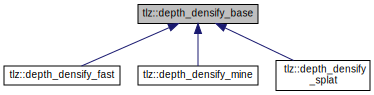
\includegraphics[width=350pt]{classtlz_1_1depth__densify__base__inherit__graph}
\end{center}
\end{figure}
\subsection*{Public Types}
\begin{DoxyCompactItemize}
\item 
using \hyperlink{classtlz_1_1depth__densify__base_a79b5945bdb65c2e1d988bf07ad730a09}{sample} = \hyperlink{structtlz_1_1ir__to__color__sample}{ir\+\_\+to\+\_\+color\+\_\+sample}$<$ \hyperlink{namespacetlz_a15fd37cce97f2b8b606af18c2615f602}{real} $>$
\end{DoxyCompactItemize}
\subsection*{Public Member Functions}
\begin{DoxyCompactItemize}
\item 
virtual \hyperlink{classtlz_1_1depth__densify__base_ad9958dcd4334e200fce135a7e59e3011}{$\sim$depth\+\_\+densify\+\_\+base} ()=default
\item 
virtual void \hyperlink{classtlz_1_1depth__densify__base_a97115be0d43315586af401293ec3c6df}{densify} (const std\+::vector$<$ \hyperlink{classtlz_1_1depth__densify__base_a79b5945bdb65c2e1d988bf07ad730a09}{sample} $>$ \&samples, cv\+::\+Mat\+\_\+$<$ \hyperlink{namespacetlz_a15fd37cce97f2b8b606af18c2615f602}{real} $>$ \&out, cv\+::\+Mat\+\_\+$<$ uchar $>$ \&out\+\_\+mask)=0
\item 
void \hyperlink{classtlz_1_1depth__densify__base_a6c61f919e71da09cc731a94fdecdaf21}{densify} (const std\+::vector$<$ \hyperlink{classtlz_1_1depth__densify__base_a79b5945bdb65c2e1d988bf07ad730a09}{sample} $>$ \&samples, cv\+::\+Mat\+\_\+$<$ \hyperlink{namespacetlz_a15fd37cce97f2b8b606af18c2615f602}{real} $>$ \&out)
\end{DoxyCompactItemize}


\subsection{Detailed Description}


Definition at line 13 of file depth\+\_\+densify.\+h.



\subsection{Member Typedef Documentation}
\index{tlz\+::depth\+\_\+densify\+\_\+base@{tlz\+::depth\+\_\+densify\+\_\+base}!sample@{sample}}
\index{sample@{sample}!tlz\+::depth\+\_\+densify\+\_\+base@{tlz\+::depth\+\_\+densify\+\_\+base}}
\subsubsection[{\texorpdfstring{sample}{sample}}]{\setlength{\rightskip}{0pt plus 5cm}using {\bf tlz\+::depth\+\_\+densify\+\_\+base\+::sample} =  {\bf ir\+\_\+to\+\_\+color\+\_\+sample}$<${\bf real}$>$}\hypertarget{classtlz_1_1depth__densify__base_a79b5945bdb65c2e1d988bf07ad730a09}{}\label{classtlz_1_1depth__densify__base_a79b5945bdb65c2e1d988bf07ad730a09}


Definition at line 15 of file depth\+\_\+densify.\+h.



\subsection{Constructor \& Destructor Documentation}
\index{tlz\+::depth\+\_\+densify\+\_\+base@{tlz\+::depth\+\_\+densify\+\_\+base}!````~depth\+\_\+densify\+\_\+base@{$\sim$depth\+\_\+densify\+\_\+base}}
\index{````~depth\+\_\+densify\+\_\+base@{$\sim$depth\+\_\+densify\+\_\+base}!tlz\+::depth\+\_\+densify\+\_\+base@{tlz\+::depth\+\_\+densify\+\_\+base}}
\subsubsection[{\texorpdfstring{$\sim$depth\+\_\+densify\+\_\+base()=default}{~depth_densify_base()=default}}]{\setlength{\rightskip}{0pt plus 5cm}virtual tlz\+::depth\+\_\+densify\+\_\+base\+::$\sim$depth\+\_\+densify\+\_\+base (
\begin{DoxyParamCaption}
{}
\end{DoxyParamCaption}
)\hspace{0.3cm}{\ttfamily [virtual]}, {\ttfamily [default]}}\hypertarget{classtlz_1_1depth__densify__base_ad9958dcd4334e200fce135a7e59e3011}{}\label{classtlz_1_1depth__densify__base_ad9958dcd4334e200fce135a7e59e3011}


\subsection{Member Function Documentation}
\index{tlz\+::depth\+\_\+densify\+\_\+base@{tlz\+::depth\+\_\+densify\+\_\+base}!densify@{densify}}
\index{densify@{densify}!tlz\+::depth\+\_\+densify\+\_\+base@{tlz\+::depth\+\_\+densify\+\_\+base}}
\subsubsection[{\texorpdfstring{densify(const std\+::vector$<$ sample $>$ \&samples, cv\+::\+Mat\+\_\+$<$ real $>$ \&out, cv\+::\+Mat\+\_\+$<$ uchar $>$ \&out\+\_\+mask)=0}{densify(const std::vector< sample > &samples, cv::Mat_< real > &out, cv::Mat_< uchar > &out_mask)=0}}]{\setlength{\rightskip}{0pt plus 5cm}virtual void tlz\+::depth\+\_\+densify\+\_\+base\+::densify (
\begin{DoxyParamCaption}
\item[{const std\+::vector$<$ {\bf sample} $>$ \&}]{samples, }
\item[{cv\+::\+Mat\+\_\+$<$ {\bf real} $>$ \&}]{out, }
\item[{cv\+::\+Mat\+\_\+$<$ uchar $>$ \&}]{out\+\_\+mask}
\end{DoxyParamCaption}
)\hspace{0.3cm}{\ttfamily [pure virtual]}}\hypertarget{classtlz_1_1depth__densify__base_a97115be0d43315586af401293ec3c6df}{}\label{classtlz_1_1depth__densify__base_a97115be0d43315586af401293ec3c6df}


Implemented in \hyperlink{classtlz_1_1depth__densify__fast_a2d2e3c128c05ce717d4e3df3fefc308e}{tlz\+::depth\+\_\+densify\+\_\+fast}, \hyperlink{classtlz_1_1depth__densify__mine_a71e64d0d4db6cd8f8f0d10d7fcbc9292}{tlz\+::depth\+\_\+densify\+\_\+mine}, and \hyperlink{classtlz_1_1depth__densify__splat_a980041db19c8ef889359bb6c3f1d5e2d}{tlz\+::depth\+\_\+densify\+\_\+splat}.

\index{tlz\+::depth\+\_\+densify\+\_\+base@{tlz\+::depth\+\_\+densify\+\_\+base}!densify@{densify}}
\index{densify@{densify}!tlz\+::depth\+\_\+densify\+\_\+base@{tlz\+::depth\+\_\+densify\+\_\+base}}
\subsubsection[{\texorpdfstring{densify(const std\+::vector$<$ sample $>$ \&samples, cv\+::\+Mat\+\_\+$<$ real $>$ \&out)}{densify(const std::vector< sample > &samples, cv::Mat_< real > &out)}}]{\setlength{\rightskip}{0pt plus 5cm}void tlz\+::depth\+\_\+densify\+\_\+base\+::densify (
\begin{DoxyParamCaption}
\item[{const std\+::vector$<$ {\bf sample} $>$ \&}]{samples, }
\item[{cv\+::\+Mat\+\_\+$<$ {\bf real} $>$ \&}]{out}
\end{DoxyParamCaption}
)}\hypertarget{classtlz_1_1depth__densify__base_a6c61f919e71da09cc731a94fdecdaf21}{}\label{classtlz_1_1depth__densify__base_a6c61f919e71da09cc731a94fdecdaf21}


Definition at line 8 of file depth\+\_\+densify.\+cc.



The documentation for this class was generated from the following files\+:\begin{DoxyCompactItemize}
\item 
src/kinect/lib/densify/\hyperlink{depth__densify_8h}{depth\+\_\+densify.\+h}\item 
src/kinect/lib/densify/\hyperlink{depth__densify_8cc}{depth\+\_\+densify.\+cc}\end{DoxyCompactItemize}

\hypertarget{classtlz_1_1depth__densify__fast}{}\section{tlz\+:\+:depth\+\_\+densify\+\_\+fast Class Reference}
\label{classtlz_1_1depth__densify__fast}\index{tlz\+::depth\+\_\+densify\+\_\+fast@{tlz\+::depth\+\_\+densify\+\_\+fast}}


{\ttfamily \#include $<$depth\+\_\+densify\+\_\+fast.\+h$>$}



Inheritance diagram for tlz\+:\+:depth\+\_\+densify\+\_\+fast\+:
\nopagebreak
\begin{figure}[H]
\begin{center}
\leavevmode
\includegraphics[width=200pt]{classtlz_1_1depth__densify__fast__inherit__graph}
\end{center}
\end{figure}


Collaboration diagram for tlz\+:\+:depth\+\_\+densify\+\_\+fast\+:
\nopagebreak
\begin{figure}[H]
\begin{center}
\leavevmode
\includegraphics[width=200pt]{classtlz_1_1depth__densify__fast__coll__graph}
\end{center}
\end{figure}
\subsection*{Public Member Functions}
\begin{DoxyCompactItemize}
\item 
void \hyperlink{classtlz_1_1depth__densify__fast_a2d2e3c128c05ce717d4e3df3fefc308e}{densify} (const std\+::vector$<$ \hyperlink{classtlz_1_1depth__densify__base_a79b5945bdb65c2e1d988bf07ad730a09}{sample} $>$ \&samples, cv\+::\+Mat\+\_\+$<$ \hyperlink{namespacetlz_a15fd37cce97f2b8b606af18c2615f602}{real} $>$ \&out, cv\+::\+Mat\+\_\+$<$ uchar $>$ \&out\+\_\+mask) override
\end{DoxyCompactItemize}
\subsection*{Additional Inherited Members}


\subsection{Detailed Description}


Definition at line 8 of file depth\+\_\+densify\+\_\+fast.\+h.



\subsection{Member Function Documentation}
\index{tlz\+::depth\+\_\+densify\+\_\+fast@{tlz\+::depth\+\_\+densify\+\_\+fast}!densify@{densify}}
\index{densify@{densify}!tlz\+::depth\+\_\+densify\+\_\+fast@{tlz\+::depth\+\_\+densify\+\_\+fast}}
\subsubsection[{\texorpdfstring{densify(const std\+::vector$<$ sample $>$ \&samples, cv\+::\+Mat\+\_\+$<$ real $>$ \&out, cv\+::\+Mat\+\_\+$<$ uchar $>$ \&out\+\_\+mask) override}{densify(const std::vector< sample > &samples, cv::Mat_< real > &out, cv::Mat_< uchar > &out_mask) override}}]{\setlength{\rightskip}{0pt plus 5cm}void tlz\+::depth\+\_\+densify\+\_\+fast\+::densify (
\begin{DoxyParamCaption}
\item[{const std\+::vector$<$ {\bf sample} $>$ \&}]{samples, }
\item[{cv\+::\+Mat\+\_\+$<$ {\bf real} $>$ \&}]{out, }
\item[{cv\+::\+Mat\+\_\+$<$ uchar $>$ \&}]{out\+\_\+mask}
\end{DoxyParamCaption}
)\hspace{0.3cm}{\ttfamily [override]}, {\ttfamily [virtual]}}\hypertarget{classtlz_1_1depth__densify__fast_a2d2e3c128c05ce717d4e3df3fefc308e}{}\label{classtlz_1_1depth__densify__fast_a2d2e3c128c05ce717d4e3df3fefc308e}


Implements \hyperlink{classtlz_1_1depth__densify__base_a97115be0d43315586af401293ec3c6df}{tlz\+::depth\+\_\+densify\+\_\+base}.



Definition at line 9 of file depth\+\_\+densify\+\_\+fast.\+cc.



The documentation for this class was generated from the following files\+:\begin{DoxyCompactItemize}
\item 
src/kinect/lib/densify/\hyperlink{depth__densify__fast_8h}{depth\+\_\+densify\+\_\+fast.\+h}\item 
src/kinect/lib/densify/\hyperlink{depth__densify__fast_8cc}{depth\+\_\+densify\+\_\+fast.\+cc}\end{DoxyCompactItemize}

\hypertarget{classtlz_1_1depth__densify__mine}{}\section{tlz\+:\+:depth\+\_\+densify\+\_\+mine Class Reference}
\label{classtlz_1_1depth__densify__mine}\index{tlz\+::depth\+\_\+densify\+\_\+mine@{tlz\+::depth\+\_\+densify\+\_\+mine}}


{\ttfamily \#include $<$depth\+\_\+densify\+\_\+mine.\+h$>$}



Inheritance diagram for tlz\+:\+:depth\+\_\+densify\+\_\+mine\+:
\nopagebreak
\begin{figure}[H]
\begin{center}
\leavevmode
\includegraphics[width=200pt]{classtlz_1_1depth__densify__mine__inherit__graph}
\end{center}
\end{figure}


Collaboration diagram for tlz\+:\+:depth\+\_\+densify\+\_\+mine\+:
\nopagebreak
\begin{figure}[H]
\begin{center}
\leavevmode
\includegraphics[width=200pt]{classtlz_1_1depth__densify__mine__coll__graph}
\end{center}
\end{figure}
\subsection*{Public Member Functions}
\begin{DoxyCompactItemize}
\item 
void \hyperlink{classtlz_1_1depth__densify__mine_a71e64d0d4db6cd8f8f0d10d7fcbc9292}{densify} (const std\+::vector$<$ \hyperlink{classtlz_1_1depth__densify__base_a79b5945bdb65c2e1d988bf07ad730a09}{sample} $>$ \&samples, cv\+::\+Mat\+\_\+$<$ \hyperlink{namespacetlz_a15fd37cce97f2b8b606af18c2615f602}{real} $>$ \&out, cv\+::\+Mat\+\_\+$<$ uchar $>$ \&out\+\_\+mask) override
\end{DoxyCompactItemize}
\subsection*{Additional Inherited Members}


\subsection{Detailed Description}


Definition at line 8 of file depth\+\_\+densify\+\_\+mine.\+h.



\subsection{Member Function Documentation}
\index{tlz\+::depth\+\_\+densify\+\_\+mine@{tlz\+::depth\+\_\+densify\+\_\+mine}!densify@{densify}}
\index{densify@{densify}!tlz\+::depth\+\_\+densify\+\_\+mine@{tlz\+::depth\+\_\+densify\+\_\+mine}}
\subsubsection[{\texorpdfstring{densify(const std\+::vector$<$ sample $>$ \&samples, cv\+::\+Mat\+\_\+$<$ real $>$ \&out, cv\+::\+Mat\+\_\+$<$ uchar $>$ \&out\+\_\+mask) override}{densify(const std::vector< sample > &samples, cv::Mat_< real > &out, cv::Mat_< uchar > &out_mask) override}}]{\setlength{\rightskip}{0pt plus 5cm}void tlz\+::depth\+\_\+densify\+\_\+mine\+::densify (
\begin{DoxyParamCaption}
\item[{const std\+::vector$<$ {\bf sample} $>$ \&}]{samples, }
\item[{cv\+::\+Mat\+\_\+$<$ {\bf real} $>$ \&}]{out, }
\item[{cv\+::\+Mat\+\_\+$<$ uchar $>$ \&}]{out\+\_\+mask}
\end{DoxyParamCaption}
)\hspace{0.3cm}{\ttfamily [override]}, {\ttfamily [virtual]}}\hypertarget{classtlz_1_1depth__densify__mine_a71e64d0d4db6cd8f8f0d10d7fcbc9292}{}\label{classtlz_1_1depth__densify__mine_a71e64d0d4db6cd8f8f0d10d7fcbc9292}


Implements \hyperlink{classtlz_1_1depth__densify__base_a97115be0d43315586af401293ec3c6df}{tlz\+::depth\+\_\+densify\+\_\+base}.



Definition at line 9 of file depth\+\_\+densify\+\_\+mine.\+cc.



The documentation for this class was generated from the following files\+:\begin{DoxyCompactItemize}
\item 
src/kinect/lib/densify/\hyperlink{depth__densify__mine_8h}{depth\+\_\+densify\+\_\+mine.\+h}\item 
src/kinect/lib/densify/\hyperlink{depth__densify__mine_8cc}{depth\+\_\+densify\+\_\+mine.\+cc}\end{DoxyCompactItemize}

\hypertarget{classtlz_1_1depth__densify__splat}{}\section{tlz\+:\+:depth\+\_\+densify\+\_\+splat Class Reference}
\label{classtlz_1_1depth__densify__splat}\index{tlz\+::depth\+\_\+densify\+\_\+splat@{tlz\+::depth\+\_\+densify\+\_\+splat}}


{\ttfamily \#include $<$depth\+\_\+densify\+\_\+splat.\+h$>$}



Inheritance diagram for tlz\+:\+:depth\+\_\+densify\+\_\+splat\+:
\nopagebreak
\begin{figure}[H]
\begin{center}
\leavevmode
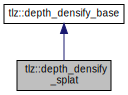
\includegraphics[width=200pt]{classtlz_1_1depth__densify__splat__inherit__graph}
\end{center}
\end{figure}


Collaboration diagram for tlz\+:\+:depth\+\_\+densify\+\_\+splat\+:
\nopagebreak
\begin{figure}[H]
\begin{center}
\leavevmode
\includegraphics[width=200pt]{classtlz_1_1depth__densify__splat__coll__graph}
\end{center}
\end{figure}
\subsection*{Public Member Functions}
\begin{DoxyCompactItemize}
\item 
void \hyperlink{classtlz_1_1depth__densify__splat_a980041db19c8ef889359bb6c3f1d5e2d}{densify} (const std\+::vector$<$ \hyperlink{classtlz_1_1depth__densify__base_a79b5945bdb65c2e1d988bf07ad730a09}{sample} $>$ \&samples, cv\+::\+Mat\+\_\+$<$ \hyperlink{namespacetlz_a15fd37cce97f2b8b606af18c2615f602}{real} $>$ \&out, cv\+::\+Mat\+\_\+$<$ uchar $>$ \&out\+\_\+mask) override
\end{DoxyCompactItemize}
\subsection*{Additional Inherited Members}


\subsection{Detailed Description}


Definition at line 8 of file depth\+\_\+densify\+\_\+splat.\+h.



\subsection{Member Function Documentation}
\index{tlz\+::depth\+\_\+densify\+\_\+splat@{tlz\+::depth\+\_\+densify\+\_\+splat}!densify@{densify}}
\index{densify@{densify}!tlz\+::depth\+\_\+densify\+\_\+splat@{tlz\+::depth\+\_\+densify\+\_\+splat}}
\subsubsection[{\texorpdfstring{densify(const std\+::vector$<$ sample $>$ \&samples, cv\+::\+Mat\+\_\+$<$ real $>$ \&out, cv\+::\+Mat\+\_\+$<$ uchar $>$ \&out\+\_\+mask) override}{densify(const std::vector< sample > &samples, cv::Mat_< real > &out, cv::Mat_< uchar > &out_mask) override}}]{\setlength{\rightskip}{0pt plus 5cm}void tlz\+::depth\+\_\+densify\+\_\+splat\+::densify (
\begin{DoxyParamCaption}
\item[{const std\+::vector$<$ {\bf sample} $>$ \&}]{samples, }
\item[{cv\+::\+Mat\+\_\+$<$ {\bf real} $>$ \&}]{out, }
\item[{cv\+::\+Mat\+\_\+$<$ uchar $>$ \&}]{out\+\_\+mask}
\end{DoxyParamCaption}
)\hspace{0.3cm}{\ttfamily [override]}, {\ttfamily [virtual]}}\hypertarget{classtlz_1_1depth__densify__splat_a980041db19c8ef889359bb6c3f1d5e2d}{}\label{classtlz_1_1depth__densify__splat_a980041db19c8ef889359bb6c3f1d5e2d}


Implements \hyperlink{classtlz_1_1depth__densify__base_a97115be0d43315586af401293ec3c6df}{tlz\+::depth\+\_\+densify\+\_\+base}.



Definition at line 9 of file depth\+\_\+densify\+\_\+splat.\+cc.



The documentation for this class was generated from the following files\+:\begin{DoxyCompactItemize}
\item 
src/kinect/lib/densify/\hyperlink{depth__densify__splat_8h}{depth\+\_\+densify\+\_\+splat.\+h}\item 
src/kinect/lib/densify/\hyperlink{depth__densify__splat_8cc}{depth\+\_\+densify\+\_\+splat.\+cc}\end{DoxyCompactItemize}

\hypertarget{structtlz_1_1kinect__reprojection__parameters_1_1depth__offset__polyfit}{}\section{tlz\+:\+:kinect\+\_\+reprojection\+\_\+parameters\+:\+:depth\+\_\+offset\+\_\+polyfit Struct Reference}
\label{structtlz_1_1kinect__reprojection__parameters_1_1depth__offset__polyfit}\index{tlz\+::kinect\+\_\+reprojection\+\_\+parameters\+::depth\+\_\+offset\+\_\+polyfit@{tlz\+::kinect\+\_\+reprojection\+\_\+parameters\+::depth\+\_\+offset\+\_\+polyfit}}


{\ttfamily \#include $<$kinect\+\_\+reprojection\+\_\+parameters.\+h$>$}

\subsection*{Public Member Functions}
\begin{DoxyCompactItemize}
\item 
\hyperlink{namespacetlz_a15fd37cce97f2b8b606af18c2615f602}{real} \hyperlink{structtlz_1_1kinect__reprojection__parameters_1_1depth__offset__polyfit_afcd41aa463d82e62efe0eee55ce2a9e3}{operator()} (\hyperlink{namespacetlz_ae192989bfbe6c700ac84d2a8cf05ebb4}{vec2} xy) const 
\item 
bool \hyperlink{structtlz_1_1kinect__reprojection__parameters_1_1depth__offset__polyfit_a265113b81e71bfb85e60a917967f10e5}{is\+\_\+none} () const 
\item 
\hyperlink{structtlz_1_1kinect__reprojection__parameters_1_1depth__offset__polyfit_ae017bf455c1487c8330e0b4214820336}{operator bool} () const 
\end{DoxyCompactItemize}
\subsection*{Public Attributes}
\begin{DoxyCompactItemize}
\item 
\hyperlink{namespacetlz_a15fd37cce97f2b8b606af18c2615f602}{real} \hyperlink{structtlz_1_1kinect__reprojection__parameters_1_1depth__offset__polyfit_aa002a6e1adfa7d4d993c967fa5e0ec04}{x0y0} = 0.\+0
\item 
\hyperlink{namespacetlz_a15fd37cce97f2b8b606af18c2615f602}{real} \hyperlink{structtlz_1_1kinect__reprojection__parameters_1_1depth__offset__polyfit_a05716b5c722f280ec0c01e203a162e97}{x1y0} = 0.\+0
\item 
\hyperlink{namespacetlz_a15fd37cce97f2b8b606af18c2615f602}{real} \hyperlink{structtlz_1_1kinect__reprojection__parameters_1_1depth__offset__polyfit_a66f698d2768cf12f59f3810fb5389cea}{x0y1} = 0.\+0
\item 
\hyperlink{namespacetlz_a15fd37cce97f2b8b606af18c2615f602}{real} \hyperlink{structtlz_1_1kinect__reprojection__parameters_1_1depth__offset__polyfit_a92b3758eeb45c26a7771827fa5ba5cfa}{x2y0} = 0.\+0
\item 
\hyperlink{namespacetlz_a15fd37cce97f2b8b606af18c2615f602}{real} \hyperlink{structtlz_1_1kinect__reprojection__parameters_1_1depth__offset__polyfit_a4c029c2acd3f81c152a52f9243ad0579}{x0y2} = 0.\+0
\item 
\hyperlink{namespacetlz_a15fd37cce97f2b8b606af18c2615f602}{real} \hyperlink{structtlz_1_1kinect__reprojection__parameters_1_1depth__offset__polyfit_ad94824250f7c6cbf3de12690bdfa29a7}{x1y1} = 0.\+0
\end{DoxyCompactItemize}


\subsection{Detailed Description}


Definition at line 11 of file kinect\+\_\+reprojection\+\_\+parameters.\+h.



\subsection{Member Function Documentation}
\index{tlz\+::kinect\+\_\+reprojection\+\_\+parameters\+::depth\+\_\+offset\+\_\+polyfit@{tlz\+::kinect\+\_\+reprojection\+\_\+parameters\+::depth\+\_\+offset\+\_\+polyfit}!is\+\_\+none@{is\+\_\+none}}
\index{is\+\_\+none@{is\+\_\+none}!tlz\+::kinect\+\_\+reprojection\+\_\+parameters\+::depth\+\_\+offset\+\_\+polyfit@{tlz\+::kinect\+\_\+reprojection\+\_\+parameters\+::depth\+\_\+offset\+\_\+polyfit}}
\subsubsection[{\texorpdfstring{is\+\_\+none() const }{is_none() const }}]{\setlength{\rightskip}{0pt plus 5cm}bool tlz\+::kinect\+\_\+reprojection\+\_\+parameters\+::depth\+\_\+offset\+\_\+polyfit\+::is\+\_\+none (
\begin{DoxyParamCaption}
{}
\end{DoxyParamCaption}
) const}\hypertarget{structtlz_1_1kinect__reprojection__parameters_1_1depth__offset__polyfit_a265113b81e71bfb85e60a917967f10e5}{}\label{structtlz_1_1kinect__reprojection__parameters_1_1depth__offset__polyfit_a265113b81e71bfb85e60a917967f10e5}


Definition at line 35 of file kinect\+\_\+reprojection\+\_\+parameters.\+cc.

\index{tlz\+::kinect\+\_\+reprojection\+\_\+parameters\+::depth\+\_\+offset\+\_\+polyfit@{tlz\+::kinect\+\_\+reprojection\+\_\+parameters\+::depth\+\_\+offset\+\_\+polyfit}!operator bool@{operator bool}}
\index{operator bool@{operator bool}!tlz\+::kinect\+\_\+reprojection\+\_\+parameters\+::depth\+\_\+offset\+\_\+polyfit@{tlz\+::kinect\+\_\+reprojection\+\_\+parameters\+::depth\+\_\+offset\+\_\+polyfit}}
\subsubsection[{\texorpdfstring{operator bool() const }{operator bool() const }}]{\setlength{\rightskip}{0pt plus 5cm}tlz\+::kinect\+\_\+reprojection\+\_\+parameters\+::depth\+\_\+offset\+\_\+polyfit\+::operator bool (
\begin{DoxyParamCaption}
{}
\end{DoxyParamCaption}
) const\hspace{0.3cm}{\ttfamily [inline]}, {\ttfamily [explicit]}}\hypertarget{structtlz_1_1kinect__reprojection__parameters_1_1depth__offset__polyfit_ae017bf455c1487c8330e0b4214820336}{}\label{structtlz_1_1kinect__reprojection__parameters_1_1depth__offset__polyfit_ae017bf455c1487c8330e0b4214820336}


Definition at line 24 of file kinect\+\_\+reprojection\+\_\+parameters.\+h.

\index{tlz\+::kinect\+\_\+reprojection\+\_\+parameters\+::depth\+\_\+offset\+\_\+polyfit@{tlz\+::kinect\+\_\+reprojection\+\_\+parameters\+::depth\+\_\+offset\+\_\+polyfit}!operator()@{operator()}}
\index{operator()@{operator()}!tlz\+::kinect\+\_\+reprojection\+\_\+parameters\+::depth\+\_\+offset\+\_\+polyfit@{tlz\+::kinect\+\_\+reprojection\+\_\+parameters\+::depth\+\_\+offset\+\_\+polyfit}}
\subsubsection[{\texorpdfstring{operator()(vec2 xy) const }{operator()(vec2 xy) const }}]{\setlength{\rightskip}{0pt plus 5cm}{\bf real} tlz\+::kinect\+\_\+reprojection\+\_\+parameters\+::depth\+\_\+offset\+\_\+polyfit\+::operator() (
\begin{DoxyParamCaption}
\item[{{\bf vec2}}]{xy}
\end{DoxyParamCaption}
) const}\hypertarget{structtlz_1_1kinect__reprojection__parameters_1_1depth__offset__polyfit_afcd41aa463d82e62efe0eee55ce2a9e3}{}\label{structtlz_1_1kinect__reprojection__parameters_1_1depth__offset__polyfit_afcd41aa463d82e62efe0eee55ce2a9e3}


Definition at line 31 of file kinect\+\_\+reprojection\+\_\+parameters.\+cc.



\subsection{Member Data Documentation}
\index{tlz\+::kinect\+\_\+reprojection\+\_\+parameters\+::depth\+\_\+offset\+\_\+polyfit@{tlz\+::kinect\+\_\+reprojection\+\_\+parameters\+::depth\+\_\+offset\+\_\+polyfit}!x0y0@{x0y0}}
\index{x0y0@{x0y0}!tlz\+::kinect\+\_\+reprojection\+\_\+parameters\+::depth\+\_\+offset\+\_\+polyfit@{tlz\+::kinect\+\_\+reprojection\+\_\+parameters\+::depth\+\_\+offset\+\_\+polyfit}}
\subsubsection[{\texorpdfstring{x0y0}{x0y0}}]{\setlength{\rightskip}{0pt plus 5cm}{\bf real} tlz\+::kinect\+\_\+reprojection\+\_\+parameters\+::depth\+\_\+offset\+\_\+polyfit\+::x0y0 = 0.\+0}\hypertarget{structtlz_1_1kinect__reprojection__parameters_1_1depth__offset__polyfit_aa002a6e1adfa7d4d993c967fa5e0ec04}{}\label{structtlz_1_1kinect__reprojection__parameters_1_1depth__offset__polyfit_aa002a6e1adfa7d4d993c967fa5e0ec04}


Definition at line 12 of file kinect\+\_\+reprojection\+\_\+parameters.\+h.

\index{tlz\+::kinect\+\_\+reprojection\+\_\+parameters\+::depth\+\_\+offset\+\_\+polyfit@{tlz\+::kinect\+\_\+reprojection\+\_\+parameters\+::depth\+\_\+offset\+\_\+polyfit}!x0y1@{x0y1}}
\index{x0y1@{x0y1}!tlz\+::kinect\+\_\+reprojection\+\_\+parameters\+::depth\+\_\+offset\+\_\+polyfit@{tlz\+::kinect\+\_\+reprojection\+\_\+parameters\+::depth\+\_\+offset\+\_\+polyfit}}
\subsubsection[{\texorpdfstring{x0y1}{x0y1}}]{\setlength{\rightskip}{0pt plus 5cm}{\bf real} tlz\+::kinect\+\_\+reprojection\+\_\+parameters\+::depth\+\_\+offset\+\_\+polyfit\+::x0y1 = 0.\+0}\hypertarget{structtlz_1_1kinect__reprojection__parameters_1_1depth__offset__polyfit_a66f698d2768cf12f59f3810fb5389cea}{}\label{structtlz_1_1kinect__reprojection__parameters_1_1depth__offset__polyfit_a66f698d2768cf12f59f3810fb5389cea}


Definition at line 15 of file kinect\+\_\+reprojection\+\_\+parameters.\+h.

\index{tlz\+::kinect\+\_\+reprojection\+\_\+parameters\+::depth\+\_\+offset\+\_\+polyfit@{tlz\+::kinect\+\_\+reprojection\+\_\+parameters\+::depth\+\_\+offset\+\_\+polyfit}!x0y2@{x0y2}}
\index{x0y2@{x0y2}!tlz\+::kinect\+\_\+reprojection\+\_\+parameters\+::depth\+\_\+offset\+\_\+polyfit@{tlz\+::kinect\+\_\+reprojection\+\_\+parameters\+::depth\+\_\+offset\+\_\+polyfit}}
\subsubsection[{\texorpdfstring{x0y2}{x0y2}}]{\setlength{\rightskip}{0pt plus 5cm}{\bf real} tlz\+::kinect\+\_\+reprojection\+\_\+parameters\+::depth\+\_\+offset\+\_\+polyfit\+::x0y2 = 0.\+0}\hypertarget{structtlz_1_1kinect__reprojection__parameters_1_1depth__offset__polyfit_a4c029c2acd3f81c152a52f9243ad0579}{}\label{structtlz_1_1kinect__reprojection__parameters_1_1depth__offset__polyfit_a4c029c2acd3f81c152a52f9243ad0579}


Definition at line 18 of file kinect\+\_\+reprojection\+\_\+parameters.\+h.

\index{tlz\+::kinect\+\_\+reprojection\+\_\+parameters\+::depth\+\_\+offset\+\_\+polyfit@{tlz\+::kinect\+\_\+reprojection\+\_\+parameters\+::depth\+\_\+offset\+\_\+polyfit}!x1y0@{x1y0}}
\index{x1y0@{x1y0}!tlz\+::kinect\+\_\+reprojection\+\_\+parameters\+::depth\+\_\+offset\+\_\+polyfit@{tlz\+::kinect\+\_\+reprojection\+\_\+parameters\+::depth\+\_\+offset\+\_\+polyfit}}
\subsubsection[{\texorpdfstring{x1y0}{x1y0}}]{\setlength{\rightskip}{0pt plus 5cm}{\bf real} tlz\+::kinect\+\_\+reprojection\+\_\+parameters\+::depth\+\_\+offset\+\_\+polyfit\+::x1y0 = 0.\+0}\hypertarget{structtlz_1_1kinect__reprojection__parameters_1_1depth__offset__polyfit_a05716b5c722f280ec0c01e203a162e97}{}\label{structtlz_1_1kinect__reprojection__parameters_1_1depth__offset__polyfit_a05716b5c722f280ec0c01e203a162e97}


Definition at line 14 of file kinect\+\_\+reprojection\+\_\+parameters.\+h.

\index{tlz\+::kinect\+\_\+reprojection\+\_\+parameters\+::depth\+\_\+offset\+\_\+polyfit@{tlz\+::kinect\+\_\+reprojection\+\_\+parameters\+::depth\+\_\+offset\+\_\+polyfit}!x1y1@{x1y1}}
\index{x1y1@{x1y1}!tlz\+::kinect\+\_\+reprojection\+\_\+parameters\+::depth\+\_\+offset\+\_\+polyfit@{tlz\+::kinect\+\_\+reprojection\+\_\+parameters\+::depth\+\_\+offset\+\_\+polyfit}}
\subsubsection[{\texorpdfstring{x1y1}{x1y1}}]{\setlength{\rightskip}{0pt plus 5cm}{\bf real} tlz\+::kinect\+\_\+reprojection\+\_\+parameters\+::depth\+\_\+offset\+\_\+polyfit\+::x1y1 = 0.\+0}\hypertarget{structtlz_1_1kinect__reprojection__parameters_1_1depth__offset__polyfit_ad94824250f7c6cbf3de12690bdfa29a7}{}\label{structtlz_1_1kinect__reprojection__parameters_1_1depth__offset__polyfit_ad94824250f7c6cbf3de12690bdfa29a7}


Definition at line 19 of file kinect\+\_\+reprojection\+\_\+parameters.\+h.

\index{tlz\+::kinect\+\_\+reprojection\+\_\+parameters\+::depth\+\_\+offset\+\_\+polyfit@{tlz\+::kinect\+\_\+reprojection\+\_\+parameters\+::depth\+\_\+offset\+\_\+polyfit}!x2y0@{x2y0}}
\index{x2y0@{x2y0}!tlz\+::kinect\+\_\+reprojection\+\_\+parameters\+::depth\+\_\+offset\+\_\+polyfit@{tlz\+::kinect\+\_\+reprojection\+\_\+parameters\+::depth\+\_\+offset\+\_\+polyfit}}
\subsubsection[{\texorpdfstring{x2y0}{x2y0}}]{\setlength{\rightskip}{0pt plus 5cm}{\bf real} tlz\+::kinect\+\_\+reprojection\+\_\+parameters\+::depth\+\_\+offset\+\_\+polyfit\+::x2y0 = 0.\+0}\hypertarget{structtlz_1_1kinect__reprojection__parameters_1_1depth__offset__polyfit_a92b3758eeb45c26a7771827fa5ba5cfa}{}\label{structtlz_1_1kinect__reprojection__parameters_1_1depth__offset__polyfit_a92b3758eeb45c26a7771827fa5ba5cfa}


Definition at line 17 of file kinect\+\_\+reprojection\+\_\+parameters.\+h.



The documentation for this struct was generated from the following files\+:\begin{DoxyCompactItemize}
\item 
src/kinect/lib/\hyperlink{kinect__reprojection__parameters_8h}{kinect\+\_\+reprojection\+\_\+parameters.\+h}\item 
src/kinect/lib/\hyperlink{kinect__reprojection__parameters_8cc}{kinect\+\_\+reprojection\+\_\+parameters.\+cc}\end{DoxyCompactItemize}

\hypertarget{structtlz_1_1distortion__parameters}{}\section{tlz\+:\+:distortion\+\_\+parameters Struct Reference}
\label{structtlz_1_1distortion__parameters}\index{tlz\+::distortion\+\_\+parameters@{tlz\+::distortion\+\_\+parameters}}


{\ttfamily \#include $<$intrinsics.\+h$>$}

\subsection*{Public Member Functions}
\begin{DoxyCompactItemize}
\item 
std\+::vector$<$ \hyperlink{namespacetlz_a15fd37cce97f2b8b606af18c2615f602}{real} $>$ \hyperlink{structtlz_1_1distortion__parameters_a96312c5d7baa4b7b1f2a76e9396037f8}{cv\+\_\+coeffs} () const 
\item 
bool \hyperlink{structtlz_1_1distortion__parameters_a307fee036b04519d633fb8456899850c}{is\+\_\+none} () const 
\item 
\hyperlink{structtlz_1_1distortion__parameters_af81eafdc705c1c91af0bfa6a6e0c7e8d}{operator bool} () const 
\end{DoxyCompactItemize}
\subsection*{Public Attributes}
\begin{DoxyCompactItemize}
\item 
\hyperlink{namespacetlz_a15fd37cce97f2b8b606af18c2615f602}{real} \hyperlink{structtlz_1_1distortion__parameters_a3763e9aa237944173a55cf42e9259662}{k1} = 0.\+0
\item 
\hyperlink{namespacetlz_a15fd37cce97f2b8b606af18c2615f602}{real} \hyperlink{structtlz_1_1distortion__parameters_af68e774f6af83517048c48a2d6880466}{k2} = 0.\+0
\item 
\hyperlink{namespacetlz_a15fd37cce97f2b8b606af18c2615f602}{real} \hyperlink{structtlz_1_1distortion__parameters_a498f99e384cb7e4e0b94eb20bdf988d6}{k3} = 0.\+0
\item 
\hyperlink{namespacetlz_a15fd37cce97f2b8b606af18c2615f602}{real} \hyperlink{structtlz_1_1distortion__parameters_a129d1ec5b0f94a1936c042d1b17a8735}{p1} = 0.\+0
\item 
\hyperlink{namespacetlz_a15fd37cce97f2b8b606af18c2615f602}{real} \hyperlink{structtlz_1_1distortion__parameters_a1869618a7c2b3438a20fc488ccf4d818}{p2} = 0.\+0
\end{DoxyCompactItemize}


\subsection{Detailed Description}


Definition at line 10 of file intrinsics.\+h.



\subsection{Member Function Documentation}
\index{tlz\+::distortion\+\_\+parameters@{tlz\+::distortion\+\_\+parameters}!cv\+\_\+coeffs@{cv\+\_\+coeffs}}
\index{cv\+\_\+coeffs@{cv\+\_\+coeffs}!tlz\+::distortion\+\_\+parameters@{tlz\+::distortion\+\_\+parameters}}
\subsubsection[{\texorpdfstring{cv\+\_\+coeffs() const }{cv_coeffs() const }}]{\setlength{\rightskip}{0pt plus 5cm}std\+::vector$<${\bf real}$>$ tlz\+::distortion\+\_\+parameters\+::cv\+\_\+coeffs (
\begin{DoxyParamCaption}
{}
\end{DoxyParamCaption}
) const\hspace{0.3cm}{\ttfamily [inline]}}\hypertarget{structtlz_1_1distortion__parameters_a96312c5d7baa4b7b1f2a76e9396037f8}{}\label{structtlz_1_1distortion__parameters_a96312c5d7baa4b7b1f2a76e9396037f8}


Definition at line 17 of file intrinsics.\+h.

\index{tlz\+::distortion\+\_\+parameters@{tlz\+::distortion\+\_\+parameters}!is\+\_\+none@{is\+\_\+none}}
\index{is\+\_\+none@{is\+\_\+none}!tlz\+::distortion\+\_\+parameters@{tlz\+::distortion\+\_\+parameters}}
\subsubsection[{\texorpdfstring{is\+\_\+none() const }{is_none() const }}]{\setlength{\rightskip}{0pt plus 5cm}bool tlz\+::distortion\+\_\+parameters\+::is\+\_\+none (
\begin{DoxyParamCaption}
{}
\end{DoxyParamCaption}
) const\hspace{0.3cm}{\ttfamily [inline]}}\hypertarget{structtlz_1_1distortion__parameters_a307fee036b04519d633fb8456899850c}{}\label{structtlz_1_1distortion__parameters_a307fee036b04519d633fb8456899850c}


Definition at line 21 of file intrinsics.\+h.

\index{tlz\+::distortion\+\_\+parameters@{tlz\+::distortion\+\_\+parameters}!operator bool@{operator bool}}
\index{operator bool@{operator bool}!tlz\+::distortion\+\_\+parameters@{tlz\+::distortion\+\_\+parameters}}
\subsubsection[{\texorpdfstring{operator bool() const }{operator bool() const }}]{\setlength{\rightskip}{0pt plus 5cm}tlz\+::distortion\+\_\+parameters\+::operator bool (
\begin{DoxyParamCaption}
{}
\end{DoxyParamCaption}
) const\hspace{0.3cm}{\ttfamily [inline]}, {\ttfamily [explicit]}}\hypertarget{structtlz_1_1distortion__parameters_af81eafdc705c1c91af0bfa6a6e0c7e8d}{}\label{structtlz_1_1distortion__parameters_af81eafdc705c1c91af0bfa6a6e0c7e8d}


Definition at line 24 of file intrinsics.\+h.



\subsection{Member Data Documentation}
\index{tlz\+::distortion\+\_\+parameters@{tlz\+::distortion\+\_\+parameters}!k1@{k1}}
\index{k1@{k1}!tlz\+::distortion\+\_\+parameters@{tlz\+::distortion\+\_\+parameters}}
\subsubsection[{\texorpdfstring{k1}{k1}}]{\setlength{\rightskip}{0pt plus 5cm}{\bf real} tlz\+::distortion\+\_\+parameters\+::k1 = 0.\+0}\hypertarget{structtlz_1_1distortion__parameters_a3763e9aa237944173a55cf42e9259662}{}\label{structtlz_1_1distortion__parameters_a3763e9aa237944173a55cf42e9259662}


Definition at line 11 of file intrinsics.\+h.

\index{tlz\+::distortion\+\_\+parameters@{tlz\+::distortion\+\_\+parameters}!k2@{k2}}
\index{k2@{k2}!tlz\+::distortion\+\_\+parameters@{tlz\+::distortion\+\_\+parameters}}
\subsubsection[{\texorpdfstring{k2}{k2}}]{\setlength{\rightskip}{0pt plus 5cm}{\bf real} tlz\+::distortion\+\_\+parameters\+::k2 = 0.\+0}\hypertarget{structtlz_1_1distortion__parameters_af68e774f6af83517048c48a2d6880466}{}\label{structtlz_1_1distortion__parameters_af68e774f6af83517048c48a2d6880466}


Definition at line 12 of file intrinsics.\+h.

\index{tlz\+::distortion\+\_\+parameters@{tlz\+::distortion\+\_\+parameters}!k3@{k3}}
\index{k3@{k3}!tlz\+::distortion\+\_\+parameters@{tlz\+::distortion\+\_\+parameters}}
\subsubsection[{\texorpdfstring{k3}{k3}}]{\setlength{\rightskip}{0pt plus 5cm}{\bf real} tlz\+::distortion\+\_\+parameters\+::k3 = 0.\+0}\hypertarget{structtlz_1_1distortion__parameters_a498f99e384cb7e4e0b94eb20bdf988d6}{}\label{structtlz_1_1distortion__parameters_a498f99e384cb7e4e0b94eb20bdf988d6}


Definition at line 13 of file intrinsics.\+h.

\index{tlz\+::distortion\+\_\+parameters@{tlz\+::distortion\+\_\+parameters}!p1@{p1}}
\index{p1@{p1}!tlz\+::distortion\+\_\+parameters@{tlz\+::distortion\+\_\+parameters}}
\subsubsection[{\texorpdfstring{p1}{p1}}]{\setlength{\rightskip}{0pt plus 5cm}{\bf real} tlz\+::distortion\+\_\+parameters\+::p1 = 0.\+0}\hypertarget{structtlz_1_1distortion__parameters_a129d1ec5b0f94a1936c042d1b17a8735}{}\label{structtlz_1_1distortion__parameters_a129d1ec5b0f94a1936c042d1b17a8735}


Definition at line 14 of file intrinsics.\+h.

\index{tlz\+::distortion\+\_\+parameters@{tlz\+::distortion\+\_\+parameters}!p2@{p2}}
\index{p2@{p2}!tlz\+::distortion\+\_\+parameters@{tlz\+::distortion\+\_\+parameters}}
\subsubsection[{\texorpdfstring{p2}{p2}}]{\setlength{\rightskip}{0pt plus 5cm}{\bf real} tlz\+::distortion\+\_\+parameters\+::p2 = 0.\+0}\hypertarget{structtlz_1_1distortion__parameters_a1869618a7c2b3438a20fc488ccf4d818}{}\label{structtlz_1_1distortion__parameters_a1869618a7c2b3438a20fc488ccf4d818}


Definition at line 15 of file intrinsics.\+h.



The documentation for this struct was generated from the following file\+:\begin{DoxyCompactItemize}
\item 
src/lib/\hyperlink{intrinsics_8h}{intrinsics.\+h}\end{DoxyCompactItemize}

\hypertarget{structestimate__relative__scale__result}{}\section{estimate\+\_\+relative\+\_\+scale\+\_\+result Struct Reference}
\label{structestimate__relative__scale__result}\index{estimate\+\_\+relative\+\_\+scale\+\_\+result@{estimate\+\_\+relative\+\_\+scale\+\_\+result}}
\subsection*{Public Member Functions}
\begin{DoxyCompactItemize}
\item 
\hyperlink{structestimate__relative__scale__result_a833176d34b4c241bd71dd3a887a4a6b0}{operator bool} () const 
\end{DoxyCompactItemize}
\subsection*{Public Attributes}
\begin{DoxyCompactItemize}
\item 
\hyperlink{namespacetlz_a15fd37cce97f2b8b606af18c2615f602}{real} \hyperlink{structestimate__relative__scale__result_ab8367cf20aa2079710e5bdbdc8962713}{scale} = N\+AN
\item 
\hyperlink{namespacetlz_a15fd37cce97f2b8b606af18c2615f602}{real} \hyperlink{structestimate__relative__scale__result_a42f8a6166b65c51e165a3c0ebca2a8d2}{weight} = 0.\+0
\end{DoxyCompactItemize}


\subsection{Detailed Description}


Definition at line 57 of file cg\+\_\+straight\+\_\+depths\+\_\+from\+\_\+disparity.\+cc.



\subsection{Member Function Documentation}
\index{estimate\+\_\+relative\+\_\+scale\+\_\+result@{estimate\+\_\+relative\+\_\+scale\+\_\+result}!operator bool@{operator bool}}
\index{operator bool@{operator bool}!estimate\+\_\+relative\+\_\+scale\+\_\+result@{estimate\+\_\+relative\+\_\+scale\+\_\+result}}
\subsubsection[{\texorpdfstring{operator bool() const }{operator bool() const }}]{\setlength{\rightskip}{0pt plus 5cm}estimate\+\_\+relative\+\_\+scale\+\_\+result\+::operator bool (
\begin{DoxyParamCaption}
{}
\end{DoxyParamCaption}
) const\hspace{0.3cm}{\ttfamily [inline]}, {\ttfamily [explicit]}}\hypertarget{structestimate__relative__scale__result_a833176d34b4c241bd71dd3a887a4a6b0}{}\label{structestimate__relative__scale__result_a833176d34b4c241bd71dd3a887a4a6b0}


Definition at line 61 of file cg\+\_\+straight\+\_\+depths\+\_\+from\+\_\+disparity.\+cc.



\subsection{Member Data Documentation}
\index{estimate\+\_\+relative\+\_\+scale\+\_\+result@{estimate\+\_\+relative\+\_\+scale\+\_\+result}!scale@{scale}}
\index{scale@{scale}!estimate\+\_\+relative\+\_\+scale\+\_\+result@{estimate\+\_\+relative\+\_\+scale\+\_\+result}}
\subsubsection[{\texorpdfstring{scale}{scale}}]{\setlength{\rightskip}{0pt plus 5cm}{\bf real} estimate\+\_\+relative\+\_\+scale\+\_\+result\+::scale = N\+AN}\hypertarget{structestimate__relative__scale__result_ab8367cf20aa2079710e5bdbdc8962713}{}\label{structestimate__relative__scale__result_ab8367cf20aa2079710e5bdbdc8962713}


Definition at line 58 of file cg\+\_\+straight\+\_\+depths\+\_\+from\+\_\+disparity.\+cc.

\index{estimate\+\_\+relative\+\_\+scale\+\_\+result@{estimate\+\_\+relative\+\_\+scale\+\_\+result}!weight@{weight}}
\index{weight@{weight}!estimate\+\_\+relative\+\_\+scale\+\_\+result@{estimate\+\_\+relative\+\_\+scale\+\_\+result}}
\subsubsection[{\texorpdfstring{weight}{weight}}]{\setlength{\rightskip}{0pt plus 5cm}{\bf real} estimate\+\_\+relative\+\_\+scale\+\_\+result\+::weight = 0.\+0}\hypertarget{structestimate__relative__scale__result_a42f8a6166b65c51e165a3c0ebca2a8d2}{}\label{structestimate__relative__scale__result_a42f8a6166b65c51e165a3c0ebca2a8d2}


Definition at line 59 of file cg\+\_\+straight\+\_\+depths\+\_\+from\+\_\+disparity.\+cc.



The documentation for this struct was generated from the following file\+:\begin{DoxyCompactItemize}
\item 
src/calibration/\hyperlink{cg__straight__depths__from__disparity_8cc}{cg\+\_\+straight\+\_\+depths\+\_\+from\+\_\+disparity.\+cc}\end{DoxyCompactItemize}

\hypertarget{classtlz_1_1failed__assertion}{}\section{tlz\+:\+:failed\+\_\+assertion Class Reference}
\label{classtlz_1_1failed__assertion}\index{tlz\+::failed\+\_\+assertion@{tlz\+::failed\+\_\+assertion}}


{\ttfamily \#include $<$assert.\+h$>$}



Inheritance diagram for tlz\+:\+:failed\+\_\+assertion\+:
\nopagebreak
\begin{figure}[H]
\begin{center}
\leavevmode
\includegraphics[width=181pt]{classtlz_1_1failed__assertion__inherit__graph}
\end{center}
\end{figure}


Collaboration diagram for tlz\+:\+:failed\+\_\+assertion\+:
\nopagebreak
\begin{figure}[H]
\begin{center}
\leavevmode
\includegraphics[width=181pt]{classtlz_1_1failed__assertion__coll__graph}
\end{center}
\end{figure}


\subsection{Detailed Description}


Definition at line 55 of file assert.\+h.



The documentation for this class was generated from the following file\+:\begin{DoxyCompactItemize}
\item 
src/lib/\hyperlink{assert_8h}{assert.\+h}\end{DoxyCompactItemize}

\hypertarget{structtlz_1_1feature__point}{}\section{tlz\+:\+:feature\+\_\+point Struct Reference}
\label{structtlz_1_1feature__point}\index{tlz\+::feature\+\_\+point@{tlz\+::feature\+\_\+point}}


{\ttfamily \#include $<$feature\+\_\+point.\+h$>$}

\subsection*{Public Member Functions}
\begin{DoxyCompactItemize}
\item 
bool \hyperlink{structtlz_1_1feature__point_a3ec9520866358aac2c5c24b3027fbe9d}{operator==} (const \hyperlink{structtlz_1_1feature__point}{feature\+\_\+point} \&other) const 
\end{DoxyCompactItemize}
\subsection*{Public Attributes}
\begin{DoxyCompactItemize}
\item 
\hyperlink{namespacetlz_ae192989bfbe6c700ac84d2a8cf05ebb4}{vec2} \hyperlink{structtlz_1_1feature__point_a841c263a06fece202e68db0144875c16}{position}
\item 
\hyperlink{namespacetlz_a15fd37cce97f2b8b606af18c2615f602}{real} \hyperlink{structtlz_1_1feature__point_a9f2ce2fe87fc8da5ba03f73663889280}{depth} = 0.\+0
\item 
\hyperlink{namespacetlz_a15fd37cce97f2b8b606af18c2615f602}{real} \hyperlink{structtlz_1_1feature__point_a3778df761d42f7fee3265ed996367ebc}{weight} = 1.\+0
\end{DoxyCompactItemize}


\subsection{Detailed Description}


Definition at line 9 of file feature\+\_\+point.\+h.



\subsection{Member Function Documentation}
\index{tlz\+::feature\+\_\+point@{tlz\+::feature\+\_\+point}!operator==@{operator==}}
\index{operator==@{operator==}!tlz\+::feature\+\_\+point@{tlz\+::feature\+\_\+point}}
\subsubsection[{\texorpdfstring{operator==(const feature\+\_\+point \&other) const }{operator==(const feature_point &other) const }}]{\setlength{\rightskip}{0pt plus 5cm}bool tlz\+::feature\+\_\+point\+::operator== (
\begin{DoxyParamCaption}
\item[{const {\bf feature\+\_\+point} \&}]{other}
\end{DoxyParamCaption}
) const\hspace{0.3cm}{\ttfamily [inline]}}\hypertarget{structtlz_1_1feature__point_a3ec9520866358aac2c5c24b3027fbe9d}{}\label{structtlz_1_1feature__point_a3ec9520866358aac2c5c24b3027fbe9d}


Definition at line 14 of file feature\+\_\+point.\+h.



\subsection{Member Data Documentation}
\index{tlz\+::feature\+\_\+point@{tlz\+::feature\+\_\+point}!depth@{depth}}
\index{depth@{depth}!tlz\+::feature\+\_\+point@{tlz\+::feature\+\_\+point}}
\subsubsection[{\texorpdfstring{depth}{depth}}]{\setlength{\rightskip}{0pt plus 5cm}{\bf real} tlz\+::feature\+\_\+point\+::depth = 0.\+0}\hypertarget{structtlz_1_1feature__point_a9f2ce2fe87fc8da5ba03f73663889280}{}\label{structtlz_1_1feature__point_a9f2ce2fe87fc8da5ba03f73663889280}


Definition at line 11 of file feature\+\_\+point.\+h.

\index{tlz\+::feature\+\_\+point@{tlz\+::feature\+\_\+point}!position@{position}}
\index{position@{position}!tlz\+::feature\+\_\+point@{tlz\+::feature\+\_\+point}}
\subsubsection[{\texorpdfstring{position}{position}}]{\setlength{\rightskip}{0pt plus 5cm}{\bf vec2} tlz\+::feature\+\_\+point\+::position}\hypertarget{structtlz_1_1feature__point_a841c263a06fece202e68db0144875c16}{}\label{structtlz_1_1feature__point_a841c263a06fece202e68db0144875c16}


Definition at line 10 of file feature\+\_\+point.\+h.

\index{tlz\+::feature\+\_\+point@{tlz\+::feature\+\_\+point}!weight@{weight}}
\index{weight@{weight}!tlz\+::feature\+\_\+point@{tlz\+::feature\+\_\+point}}
\subsubsection[{\texorpdfstring{weight}{weight}}]{\setlength{\rightskip}{0pt plus 5cm}{\bf real} tlz\+::feature\+\_\+point\+::weight = 1.\+0}\hypertarget{structtlz_1_1feature__point_a3778df761d42f7fee3265ed996367ebc}{}\label{structtlz_1_1feature__point_a3778df761d42f7fee3265ed996367ebc}


Definition at line 12 of file feature\+\_\+point.\+h.



The documentation for this struct was generated from the following file\+:\begin{DoxyCompactItemize}
\item 
src/calibration/lib/\hyperlink{feature__point_8h}{feature\+\_\+point.\+h}\end{DoxyCompactItemize}

\hypertarget{structtlz_1_1feature__points}{}\section{tlz\+:\+:feature\+\_\+points Struct Reference}
\label{structtlz_1_1feature__points}\index{tlz\+::feature\+\_\+points@{tlz\+::feature\+\_\+points}}


Points of different features, on one view.  




{\ttfamily \#include $<$feature\+\_\+points.\+h$>$}



Inheritance diagram for tlz\+:\+:feature\+\_\+points\+:
\nopagebreak
\begin{figure}[H]
\begin{center}
\leavevmode
\includegraphics[width=177pt]{structtlz_1_1feature__points__inherit__graph}
\end{center}
\end{figure}


Collaboration diagram for tlz\+:\+:feature\+\_\+points\+:
\nopagebreak
\begin{figure}[H]
\begin{center}
\leavevmode
\includegraphics[width=175pt]{structtlz_1_1feature__points__coll__graph}
\end{center}
\end{figure}
\subsection*{Public Member Functions}
\begin{DoxyCompactItemize}
\item 
bool \hyperlink{structtlz_1_1feature__points_a6fe789104ca6d9ef42d9bfd08e147f94}{has\+\_\+feature} (const std\+::string \&feature\+\_\+name) const 
\item 
std\+::size\+\_\+t \hyperlink{structtlz_1_1feature__points_a9ab42a1839b4826e689d7eb32e24474d}{count} () const 
\item 
void \hyperlink{structtlz_1_1feature__points_a6e84713a19d756fd342b47b2685ef84a}{normalize\+\_\+weights} ()
\end{DoxyCompactItemize}
\subsection*{Public Attributes}
\begin{DoxyCompactItemize}
\item 
std\+::map$<$ std\+::string, \hyperlink{structtlz_1_1feature__point}{feature\+\_\+point} $>$ \hyperlink{structtlz_1_1feature__points_a6a8a228f04b6decf87126a0fc4194e57}{points}
\item 
\hyperlink{structtlz_1_1view__index}{view\+\_\+index} \hyperlink{structtlz_1_1feature__points_ad267674b24423a95053c47ee371f78d6}{view\+\_\+idx}
\item 
bool \hyperlink{structtlz_1_1feature__points_a12753624989e36296202481e4f8f4147}{is\+\_\+distorted} = false
\end{DoxyCompactItemize}


\subsection{Detailed Description}
Points of different features, on one view. 

Definition at line 18 of file feature\+\_\+points.\+h.



\subsection{Member Function Documentation}
\index{tlz\+::feature\+\_\+points@{tlz\+::feature\+\_\+points}!count@{count}}
\index{count@{count}!tlz\+::feature\+\_\+points@{tlz\+::feature\+\_\+points}}
\subsubsection[{\texorpdfstring{count() const }{count() const }}]{\setlength{\rightskip}{0pt plus 5cm}std\+::size\+\_\+t tlz\+::feature\+\_\+points\+::count (
\begin{DoxyParamCaption}
{}
\end{DoxyParamCaption}
) const\hspace{0.3cm}{\ttfamily [inline]}}\hypertarget{structtlz_1_1feature__points_a9ab42a1839b4826e689d7eb32e24474d}{}\label{structtlz_1_1feature__points_a9ab42a1839b4826e689d7eb32e24474d}


Definition at line 26 of file feature\+\_\+points.\+h.

\index{tlz\+::feature\+\_\+points@{tlz\+::feature\+\_\+points}!has\+\_\+feature@{has\+\_\+feature}}
\index{has\+\_\+feature@{has\+\_\+feature}!tlz\+::feature\+\_\+points@{tlz\+::feature\+\_\+points}}
\subsubsection[{\texorpdfstring{has\+\_\+feature(const std\+::string \&feature\+\_\+name) const }{has_feature(const std::string &feature_name) const }}]{\setlength{\rightskip}{0pt plus 5cm}bool tlz\+::feature\+\_\+points\+::has\+\_\+feature (
\begin{DoxyParamCaption}
\item[{const std\+::string \&}]{feature\+\_\+name}
\end{DoxyParamCaption}
) const\hspace{0.3cm}{\ttfamily [inline]}}\hypertarget{structtlz_1_1feature__points_a6fe789104ca6d9ef42d9bfd08e147f94}{}\label{structtlz_1_1feature__points_a6fe789104ca6d9ef42d9bfd08e147f94}


Definition at line 23 of file feature\+\_\+points.\+h.

\index{tlz\+::feature\+\_\+points@{tlz\+::feature\+\_\+points}!normalize\+\_\+weights@{normalize\+\_\+weights}}
\index{normalize\+\_\+weights@{normalize\+\_\+weights}!tlz\+::feature\+\_\+points@{tlz\+::feature\+\_\+points}}
\subsubsection[{\texorpdfstring{normalize\+\_\+weights()}{normalize_weights()}}]{\setlength{\rightskip}{0pt plus 5cm}void tlz\+::feature\+\_\+points\+::normalize\+\_\+weights (
\begin{DoxyParamCaption}
{}
\end{DoxyParamCaption}
)}\hypertarget{structtlz_1_1feature__points_a6e84713a19d756fd342b47b2685ef84a}{}\label{structtlz_1_1feature__points_a6e84713a19d756fd342b47b2685ef84a}


Definition at line 41 of file feature\+\_\+points.\+cc.



\subsection{Member Data Documentation}
\index{tlz\+::feature\+\_\+points@{tlz\+::feature\+\_\+points}!is\+\_\+distorted@{is\+\_\+distorted}}
\index{is\+\_\+distorted@{is\+\_\+distorted}!tlz\+::feature\+\_\+points@{tlz\+::feature\+\_\+points}}
\subsubsection[{\texorpdfstring{is\+\_\+distorted}{is_distorted}}]{\setlength{\rightskip}{0pt plus 5cm}bool tlz\+::feature\+\_\+points\+::is\+\_\+distorted = false}\hypertarget{structtlz_1_1feature__points_a12753624989e36296202481e4f8f4147}{}\label{structtlz_1_1feature__points_a12753624989e36296202481e4f8f4147}


Definition at line 21 of file feature\+\_\+points.\+h.

\index{tlz\+::feature\+\_\+points@{tlz\+::feature\+\_\+points}!points@{points}}
\index{points@{points}!tlz\+::feature\+\_\+points@{tlz\+::feature\+\_\+points}}
\subsubsection[{\texorpdfstring{points}{points}}]{\setlength{\rightskip}{0pt plus 5cm}std\+::map$<$std\+::string, {\bf feature\+\_\+point}$>$ tlz\+::feature\+\_\+points\+::points}\hypertarget{structtlz_1_1feature__points_a6a8a228f04b6decf87126a0fc4194e57}{}\label{structtlz_1_1feature__points_a6a8a228f04b6decf87126a0fc4194e57}


Definition at line 19 of file feature\+\_\+points.\+h.

\index{tlz\+::feature\+\_\+points@{tlz\+::feature\+\_\+points}!view\+\_\+idx@{view\+\_\+idx}}
\index{view\+\_\+idx@{view\+\_\+idx}!tlz\+::feature\+\_\+points@{tlz\+::feature\+\_\+points}}
\subsubsection[{\texorpdfstring{view\+\_\+idx}{view_idx}}]{\setlength{\rightskip}{0pt plus 5cm}{\bf view\+\_\+index} tlz\+::feature\+\_\+points\+::view\+\_\+idx}\hypertarget{structtlz_1_1feature__points_ad267674b24423a95053c47ee371f78d6}{}\label{structtlz_1_1feature__points_ad267674b24423a95053c47ee371f78d6}


Definition at line 20 of file feature\+\_\+points.\+h.



The documentation for this struct was generated from the following files\+:\begin{DoxyCompactItemize}
\item 
src/calibration/lib/\hyperlink{feature__points_8h}{feature\+\_\+points.\+h}\item 
src/calibration/lib/\hyperlink{feature__points_8cc}{feature\+\_\+points.\+cc}\end{DoxyCompactItemize}

\hypertarget{structtlz_1_1feature__slope}{}\section{tlz\+:\+:feature\+\_\+slope Struct Reference}
\label{structtlz_1_1feature__slope}\index{tlz\+::feature\+\_\+slope@{tlz\+::feature\+\_\+slope}}


{\ttfamily \#include $<$feature\+\_\+slopes.\+h$>$}

\subsection*{Public Attributes}
\begin{DoxyCompactItemize}
\item 
\hyperlink{namespacetlz_a15fd37cce97f2b8b606af18c2615f602}{real} \hyperlink{structtlz_1_1feature__slope_af8685842a790e87ae4bed5a358b68e97}{horizontal} = N\+AN
\item 
\hyperlink{namespacetlz_a15fd37cce97f2b8b606af18c2615f602}{real} \hyperlink{structtlz_1_1feature__slope_a5dce39e1652c504075245a3e6c2decfc}{vertical} = N\+AN
\end{DoxyCompactItemize}


\subsection{Detailed Description}


Definition at line 14 of file feature\+\_\+slopes.\+h.



\subsection{Member Data Documentation}
\index{tlz\+::feature\+\_\+slope@{tlz\+::feature\+\_\+slope}!horizontal@{horizontal}}
\index{horizontal@{horizontal}!tlz\+::feature\+\_\+slope@{tlz\+::feature\+\_\+slope}}
\subsubsection[{\texorpdfstring{horizontal}{horizontal}}]{\setlength{\rightskip}{0pt plus 5cm}{\bf real} tlz\+::feature\+\_\+slope\+::horizontal = N\+AN}\hypertarget{structtlz_1_1feature__slope_af8685842a790e87ae4bed5a358b68e97}{}\label{structtlz_1_1feature__slope_af8685842a790e87ae4bed5a358b68e97}


Definition at line 15 of file feature\+\_\+slopes.\+h.

\index{tlz\+::feature\+\_\+slope@{tlz\+::feature\+\_\+slope}!vertical@{vertical}}
\index{vertical@{vertical}!tlz\+::feature\+\_\+slope@{tlz\+::feature\+\_\+slope}}
\subsubsection[{\texorpdfstring{vertical}{vertical}}]{\setlength{\rightskip}{0pt plus 5cm}{\bf real} tlz\+::feature\+\_\+slope\+::vertical = N\+AN}\hypertarget{structtlz_1_1feature__slope_a5dce39e1652c504075245a3e6c2decfc}{}\label{structtlz_1_1feature__slope_a5dce39e1652c504075245a3e6c2decfc}


Definition at line 16 of file feature\+\_\+slopes.\+h.



The documentation for this struct was generated from the following file\+:\begin{DoxyCompactItemize}
\item 
src/calibration/lib/cg/\hyperlink{feature__slopes_8h}{feature\+\_\+slopes.\+h}\end{DoxyCompactItemize}

\hypertarget{structtlz_1_1feature__slopes}{}\section{tlz\+:\+:feature\+\_\+slopes Struct Reference}
\label{structtlz_1_1feature__slopes}\index{tlz\+::feature\+\_\+slopes@{tlz\+::feature\+\_\+slopes}}


{\ttfamily \#include $<$feature\+\_\+slopes.\+h$>$}



Inheritance diagram for tlz\+:\+:feature\+\_\+slopes\+:
\nopagebreak
\begin{figure}[H]
\begin{center}
\leavevmode
\includegraphics[width=177pt]{structtlz_1_1feature__slopes__inherit__graph}
\end{center}
\end{figure}


Collaboration diagram for tlz\+:\+:feature\+\_\+slopes\+:
\nopagebreak
\begin{figure}[H]
\begin{center}
\leavevmode
\includegraphics[width=177pt]{structtlz_1_1feature__slopes__coll__graph}
\end{center}
\end{figure}
\subsection*{Public Member Functions}
\begin{DoxyCompactItemize}
\item 
\hyperlink{structtlz_1_1feature__slopes_a597c9368b2ced8c89508900d784a39c6}{feature\+\_\+slopes} ()=default
\item 
\hyperlink{structtlz_1_1feature__slopes_ade2ebdbc28b1b9225226998c9a862237}{feature\+\_\+slopes} (const \hyperlink{structtlz_1_1feature__points}{feature\+\_\+points} \&)
\end{DoxyCompactItemize}
\subsection*{Public Attributes}
\begin{DoxyCompactItemize}
\item 
std\+::map$<$ std\+::string, \hyperlink{structtlz_1_1feature__slope}{feature\+\_\+slope} $>$ \hyperlink{structtlz_1_1feature__slopes_a99e7abc818acbd620f93ec7b9be1eb16}{slopes}
\end{DoxyCompactItemize}


\subsection{Detailed Description}


Definition at line 18 of file feature\+\_\+slopes.\+h.



\subsection{Constructor \& Destructor Documentation}
\index{tlz\+::feature\+\_\+slopes@{tlz\+::feature\+\_\+slopes}!feature\+\_\+slopes@{feature\+\_\+slopes}}
\index{feature\+\_\+slopes@{feature\+\_\+slopes}!tlz\+::feature\+\_\+slopes@{tlz\+::feature\+\_\+slopes}}
\subsubsection[{\texorpdfstring{feature\+\_\+slopes()=default}{feature_slopes()=default}}]{\setlength{\rightskip}{0pt plus 5cm}tlz\+::feature\+\_\+slopes\+::feature\+\_\+slopes (
\begin{DoxyParamCaption}
{}
\end{DoxyParamCaption}
)\hspace{0.3cm}{\ttfamily [default]}}\hypertarget{structtlz_1_1feature__slopes_a597c9368b2ced8c89508900d784a39c6}{}\label{structtlz_1_1feature__slopes_a597c9368b2ced8c89508900d784a39c6}
\index{tlz\+::feature\+\_\+slopes@{tlz\+::feature\+\_\+slopes}!feature\+\_\+slopes@{feature\+\_\+slopes}}
\index{feature\+\_\+slopes@{feature\+\_\+slopes}!tlz\+::feature\+\_\+slopes@{tlz\+::feature\+\_\+slopes}}
\subsubsection[{\texorpdfstring{feature\+\_\+slopes(const feature\+\_\+points \&)}{feature_slopes(const feature_points &)}}]{\setlength{\rightskip}{0pt plus 5cm}tlz\+::feature\+\_\+slopes\+::feature\+\_\+slopes (
\begin{DoxyParamCaption}
\item[{const {\bf feature\+\_\+points} \&}]{fpoints}
\end{DoxyParamCaption}
)\hspace{0.3cm}{\ttfamily [explicit]}}\hypertarget{structtlz_1_1feature__slopes_ade2ebdbc28b1b9225226998c9a862237}{}\label{structtlz_1_1feature__slopes_ade2ebdbc28b1b9225226998c9a862237}


Definition at line 9 of file feature\+\_\+slopes.\+cc.



\subsection{Member Data Documentation}
\index{tlz\+::feature\+\_\+slopes@{tlz\+::feature\+\_\+slopes}!slopes@{slopes}}
\index{slopes@{slopes}!tlz\+::feature\+\_\+slopes@{tlz\+::feature\+\_\+slopes}}
\subsubsection[{\texorpdfstring{slopes}{slopes}}]{\setlength{\rightskip}{0pt plus 5cm}std\+::map$<$std\+::string, {\bf feature\+\_\+slope}$>$ tlz\+::feature\+\_\+slopes\+::slopes}\hypertarget{structtlz_1_1feature__slopes_a99e7abc818acbd620f93ec7b9be1eb16}{}\label{structtlz_1_1feature__slopes_a99e7abc818acbd620f93ec7b9be1eb16}


Definition at line 22 of file feature\+\_\+slopes.\+h.



The documentation for this struct was generated from the following files\+:\begin{DoxyCompactItemize}
\item 
src/calibration/lib/cg/\hyperlink{feature__slopes_8h}{feature\+\_\+slopes.\+h}\item 
src/calibration/lib/cg/\hyperlink{feature__slopes_8cc}{feature\+\_\+slopes.\+cc}\end{DoxyCompactItemize}

\hypertarget{structflow__state}{}\section{flow\+\_\+state Struct Reference}
\label{structflow__state}\index{flow\+\_\+state@{flow\+\_\+state}}


Collaboration diagram for flow\+\_\+state\+:
\nopagebreak
\begin{figure}[H]
\begin{center}
\leavevmode
\includegraphics[width=163pt]{structflow__state__coll__graph}
\end{center}
\end{figure}
\subsection*{Public Member Functions}
\begin{DoxyCompactItemize}
\item 
\hyperlink{structflow__state_a7f44e3a4701be71718b470f0f133dce5}{flow\+\_\+state} ()=default
\item 
\hyperlink{structflow__state_a9cca42e1283a846ee639d3f9fd0569ff}{flow\+\_\+state} (const \hyperlink{structtlz_1_1view__index}{view\+\_\+index} \&idx, const cv\+::\+Mat\+\_\+$<$ uchar $>$ \&img, std\+::size\+\_\+t \hyperlink{structflow__state_a04a62f8006f54b559ef6fcc25b87e66b}{features\+\_\+count})
\item 
std\+::size\+\_\+t \hyperlink{structflow__state_a04a62f8006f54b559ef6fcc25b87e66b}{features\+\_\+count} () const 
\item 
std\+::size\+\_\+t \hyperlink{structflow__state_a70ebb1f3987cbd90e1fd2666a0b68cf5}{valid\+\_\+features\+\_\+count} () const 
\item 
bool \hyperlink{structflow__state_ac8be37941073fba44d3bd34de142a9e4}{is\+\_\+valid} () const 
\end{DoxyCompactItemize}
\subsection*{Public Attributes}
\begin{DoxyCompactItemize}
\item 
\hyperlink{structtlz_1_1view__index}{view\+\_\+index} \hyperlink{structflow__state_acec6eb589835df528397b781483bf477}{view\+\_\+idx}
\item 
std\+::vector$<$ cv\+::\+Mat\+\_\+$<$ uchar $>$ $>$ \hyperlink{structflow__state_a83570bddb99be6487a926cab5735cff5}{image\+\_\+pyramid}
\item 
std\+::vector$<$ cv\+::\+Point2f $>$ \hyperlink{structflow__state_ac30b8c82b7f7f10fa99304293ce6b14b}{feature\+\_\+positions}
\item 
std\+::vector$<$ uchar $>$ \hyperlink{structflow__state_afe1e6db4eac958ecc432ee6c20d4e2b5}{feature\+\_\+status}
\end{DoxyCompactItemize}


\subsection{Detailed Description}


Definition at line 30 of file cg\+\_\+optical\+\_\+flow\+\_\+cors.\+cc.



\subsection{Constructor \& Destructor Documentation}
\index{flow\+\_\+state@{flow\+\_\+state}!flow\+\_\+state@{flow\+\_\+state}}
\index{flow\+\_\+state@{flow\+\_\+state}!flow\+\_\+state@{flow\+\_\+state}}
\subsubsection[{\texorpdfstring{flow\+\_\+state()=default}{flow_state()=default}}]{\setlength{\rightskip}{0pt plus 5cm}flow\+\_\+state\+::flow\+\_\+state (
\begin{DoxyParamCaption}
{}
\end{DoxyParamCaption}
)\hspace{0.3cm}{\ttfamily [default]}}\hypertarget{structflow__state_a7f44e3a4701be71718b470f0f133dce5}{}\label{structflow__state_a7f44e3a4701be71718b470f0f133dce5}
\index{flow\+\_\+state@{flow\+\_\+state}!flow\+\_\+state@{flow\+\_\+state}}
\index{flow\+\_\+state@{flow\+\_\+state}!flow\+\_\+state@{flow\+\_\+state}}
\subsubsection[{\texorpdfstring{flow\+\_\+state(const view\+\_\+index \&idx, const cv\+::\+Mat\+\_\+$<$ uchar $>$ \&img, std\+::size\+\_\+t features\+\_\+count)}{flow_state(const view_index &idx, const cv::Mat_< uchar > &img, std::size_t features_count)}}]{\setlength{\rightskip}{0pt plus 5cm}flow\+\_\+state\+::flow\+\_\+state (
\begin{DoxyParamCaption}
\item[{const {\bf view\+\_\+index} \&}]{idx, }
\item[{const cv\+::\+Mat\+\_\+$<$ uchar $>$ \&}]{img, }
\item[{std\+::size\+\_\+t}]{features\+\_\+count}
\end{DoxyParamCaption}
)\hspace{0.3cm}{\ttfamily [inline]}}\hypertarget{structflow__state_a9cca42e1283a846ee639d3f9fd0569ff}{}\label{structflow__state_a9cca42e1283a846ee639d3f9fd0569ff}


Definition at line 37 of file cg\+\_\+optical\+\_\+flow\+\_\+cors.\+cc.



\subsection{Member Function Documentation}
\index{flow\+\_\+state@{flow\+\_\+state}!features\+\_\+count@{features\+\_\+count}}
\index{features\+\_\+count@{features\+\_\+count}!flow\+\_\+state@{flow\+\_\+state}}
\subsubsection[{\texorpdfstring{features\+\_\+count() const }{features_count() const }}]{\setlength{\rightskip}{0pt plus 5cm}std\+::size\+\_\+t flow\+\_\+state\+::features\+\_\+count (
\begin{DoxyParamCaption}
{}
\end{DoxyParamCaption}
) const\hspace{0.3cm}{\ttfamily [inline]}}\hypertarget{structflow__state_a04a62f8006f54b559ef6fcc25b87e66b}{}\label{structflow__state_a04a62f8006f54b559ef6fcc25b87e66b}


Definition at line 43 of file cg\+\_\+optical\+\_\+flow\+\_\+cors.\+cc.

\index{flow\+\_\+state@{flow\+\_\+state}!is\+\_\+valid@{is\+\_\+valid}}
\index{is\+\_\+valid@{is\+\_\+valid}!flow\+\_\+state@{flow\+\_\+state}}
\subsubsection[{\texorpdfstring{is\+\_\+valid() const }{is_valid() const }}]{\setlength{\rightskip}{0pt plus 5cm}bool flow\+\_\+state\+::is\+\_\+valid (
\begin{DoxyParamCaption}
{}
\end{DoxyParamCaption}
) const\hspace{0.3cm}{\ttfamily [inline]}}\hypertarget{structflow__state_ac8be37941073fba44d3bd34de142a9e4}{}\label{structflow__state_ac8be37941073fba44d3bd34de142a9e4}


Definition at line 45 of file cg\+\_\+optical\+\_\+flow\+\_\+cors.\+cc.

\index{flow\+\_\+state@{flow\+\_\+state}!valid\+\_\+features\+\_\+count@{valid\+\_\+features\+\_\+count}}
\index{valid\+\_\+features\+\_\+count@{valid\+\_\+features\+\_\+count}!flow\+\_\+state@{flow\+\_\+state}}
\subsubsection[{\texorpdfstring{valid\+\_\+features\+\_\+count() const }{valid_features_count() const }}]{\setlength{\rightskip}{0pt plus 5cm}std\+::size\+\_\+t flow\+\_\+state\+::valid\+\_\+features\+\_\+count (
\begin{DoxyParamCaption}
{}
\end{DoxyParamCaption}
) const}\hypertarget{structflow__state_a70ebb1f3987cbd90e1fd2666a0b68cf5}{}\label{structflow__state_a70ebb1f3987cbd90e1fd2666a0b68cf5}


Definition at line 48 of file cg\+\_\+optical\+\_\+flow\+\_\+cors.\+cc.



\subsection{Member Data Documentation}
\index{flow\+\_\+state@{flow\+\_\+state}!feature\+\_\+positions@{feature\+\_\+positions}}
\index{feature\+\_\+positions@{feature\+\_\+positions}!flow\+\_\+state@{flow\+\_\+state}}
\subsubsection[{\texorpdfstring{feature\+\_\+positions}{feature_positions}}]{\setlength{\rightskip}{0pt plus 5cm}std\+::vector$<$cv\+::\+Point2f$>$ flow\+\_\+state\+::feature\+\_\+positions}\hypertarget{structflow__state_ac30b8c82b7f7f10fa99304293ce6b14b}{}\label{structflow__state_ac30b8c82b7f7f10fa99304293ce6b14b}


Definition at line 33 of file cg\+\_\+optical\+\_\+flow\+\_\+cors.\+cc.

\index{flow\+\_\+state@{flow\+\_\+state}!feature\+\_\+status@{feature\+\_\+status}}
\index{feature\+\_\+status@{feature\+\_\+status}!flow\+\_\+state@{flow\+\_\+state}}
\subsubsection[{\texorpdfstring{feature\+\_\+status}{feature_status}}]{\setlength{\rightskip}{0pt plus 5cm}std\+::vector$<$uchar$>$ flow\+\_\+state\+::feature\+\_\+status}\hypertarget{structflow__state_afe1e6db4eac958ecc432ee6c20d4e2b5}{}\label{structflow__state_afe1e6db4eac958ecc432ee6c20d4e2b5}


Definition at line 34 of file cg\+\_\+optical\+\_\+flow\+\_\+cors.\+cc.

\index{flow\+\_\+state@{flow\+\_\+state}!image\+\_\+pyramid@{image\+\_\+pyramid}}
\index{image\+\_\+pyramid@{image\+\_\+pyramid}!flow\+\_\+state@{flow\+\_\+state}}
\subsubsection[{\texorpdfstring{image\+\_\+pyramid}{image_pyramid}}]{\setlength{\rightskip}{0pt plus 5cm}std\+::vector$<$cv\+::\+Mat\+\_\+$<$uchar$>$ $>$ flow\+\_\+state\+::image\+\_\+pyramid}\hypertarget{structflow__state_a83570bddb99be6487a926cab5735cff5}{}\label{structflow__state_a83570bddb99be6487a926cab5735cff5}


Definition at line 32 of file cg\+\_\+optical\+\_\+flow\+\_\+cors.\+cc.

\index{flow\+\_\+state@{flow\+\_\+state}!view\+\_\+idx@{view\+\_\+idx}}
\index{view\+\_\+idx@{view\+\_\+idx}!flow\+\_\+state@{flow\+\_\+state}}
\subsubsection[{\texorpdfstring{view\+\_\+idx}{view_idx}}]{\setlength{\rightskip}{0pt plus 5cm}{\bf view\+\_\+index} flow\+\_\+state\+::view\+\_\+idx}\hypertarget{structflow__state_acec6eb589835df528397b781483bf477}{}\label{structflow__state_acec6eb589835df528397b781483bf477}


Definition at line 31 of file cg\+\_\+optical\+\_\+flow\+\_\+cors.\+cc.



The documentation for this struct was generated from the following file\+:\begin{DoxyCompactItemize}
\item 
src/calibration/\hyperlink{cg__optical__flow__cors_8cc}{cg\+\_\+optical\+\_\+flow\+\_\+cors.\+cc}\end{DoxyCompactItemize}

\hypertarget{classslice_1_1FormatDict}{}\section{slice.\+Format\+Dict Class Reference}
\label{classslice_1_1FormatDict}\index{slice.\+Format\+Dict@{slice.\+Format\+Dict}}


Inheritance diagram for slice.\+Format\+Dict\+:
\nopagebreak
\begin{figure}[H]
\begin{center}
\leavevmode
\includegraphics[width=169pt]{classslice_1_1FormatDict__inherit__graph}
\end{center}
\end{figure}


Collaboration diagram for slice.\+Format\+Dict\+:
\nopagebreak
\begin{figure}[H]
\begin{center}
\leavevmode
\includegraphics[width=169pt]{classslice_1_1FormatDict__coll__graph}
\end{center}
\end{figure}
\subsection*{Public Member Functions}
\begin{DoxyCompactItemize}
\item 
def \hyperlink{classslice_1_1FormatDict_ae52115baca1ece50a20c7e254e3b75ab}{\+\_\+\+\_\+missing\+\_\+\+\_\+} (self, key)
\end{DoxyCompactItemize}


\subsection{Detailed Description}


Definition at line 14 of file slice.\+py.



\subsection{Member Function Documentation}
\index{slice\+::\+Format\+Dict@{slice\+::\+Format\+Dict}!\+\_\+\+\_\+missing\+\_\+\+\_\+@{\+\_\+\+\_\+missing\+\_\+\+\_\+}}
\index{\+\_\+\+\_\+missing\+\_\+\+\_\+@{\+\_\+\+\_\+missing\+\_\+\+\_\+}!slice\+::\+Format\+Dict@{slice\+::\+Format\+Dict}}
\subsubsection[{\texorpdfstring{\+\_\+\+\_\+missing\+\_\+\+\_\+(self, key)}{__missing__(self, key)}}]{\setlength{\rightskip}{0pt plus 5cm}def slice.\+Format\+Dict.\+\_\+\+\_\+missing\+\_\+\+\_\+ (
\begin{DoxyParamCaption}
\item[{}]{self, }
\item[{}]{key}
\end{DoxyParamCaption}
)}\hypertarget{classslice_1_1FormatDict_ae52115baca1ece50a20c7e254e3b75ab}{}\label{classslice_1_1FormatDict_ae52115baca1ece50a20c7e254e3b75ab}


Definition at line 15 of file slice.\+py.



The documentation for this class was generated from the following file\+:\begin{DoxyCompactItemize}
\item 
src/dataset/\hyperlink{slice_8py}{slice.\+py}\end{DoxyCompactItemize}

\hypertarget{classflip_1_1FormatDict}{}\section{flip.\+Format\+Dict Class Reference}
\label{classflip_1_1FormatDict}\index{flip.\+Format\+Dict@{flip.\+Format\+Dict}}


Inheritance diagram for flip.\+Format\+Dict\+:
\nopagebreak
\begin{figure}[H]
\begin{center}
\leavevmode
\includegraphics[width=161pt]{classflip_1_1FormatDict__inherit__graph}
\end{center}
\end{figure}


Collaboration diagram for flip.\+Format\+Dict\+:
\nopagebreak
\begin{figure}[H]
\begin{center}
\leavevmode
\includegraphics[width=161pt]{classflip_1_1FormatDict__coll__graph}
\end{center}
\end{figure}
\subsection*{Public Member Functions}
\begin{DoxyCompactItemize}
\item 
def \hyperlink{classflip_1_1FormatDict_a646799a97ea8cbc6a840c94eb0abee3f}{\+\_\+\+\_\+missing\+\_\+\+\_\+} (self, key)
\end{DoxyCompactItemize}


\subsection{Detailed Description}


Definition at line 19 of file flip.\+py.



\subsection{Member Function Documentation}
\index{flip\+::\+Format\+Dict@{flip\+::\+Format\+Dict}!\+\_\+\+\_\+missing\+\_\+\+\_\+@{\+\_\+\+\_\+missing\+\_\+\+\_\+}}
\index{\+\_\+\+\_\+missing\+\_\+\+\_\+@{\+\_\+\+\_\+missing\+\_\+\+\_\+}!flip\+::\+Format\+Dict@{flip\+::\+Format\+Dict}}
\subsubsection[{\texorpdfstring{\+\_\+\+\_\+missing\+\_\+\+\_\+(self, key)}{__missing__(self, key)}}]{\setlength{\rightskip}{0pt plus 5cm}def flip.\+Format\+Dict.\+\_\+\+\_\+missing\+\_\+\+\_\+ (
\begin{DoxyParamCaption}
\item[{}]{self, }
\item[{}]{key}
\end{DoxyParamCaption}
)}\hypertarget{classflip_1_1FormatDict_a646799a97ea8cbc6a840c94eb0abee3f}{}\label{classflip_1_1FormatDict_a646799a97ea8cbc6a840c94eb0abee3f}


Definition at line 20 of file flip.\+py.



The documentation for this class was generated from the following file\+:\begin{DoxyCompactItemize}
\item 
src/dataset/\hyperlink{flip_8py}{flip.\+py}\end{DoxyCompactItemize}

\hypertarget{classflip_1_1FormatPlaceholder}{}\section{flip.\+Format\+Placeholder Class Reference}
\label{classflip_1_1FormatPlaceholder}\index{flip.\+Format\+Placeholder@{flip.\+Format\+Placeholder}}
\subsection*{Public Member Functions}
\begin{DoxyCompactItemize}
\item 
def \hyperlink{classflip_1_1FormatPlaceholder_ad50c387cf9532c99e733e5c711374bfd}{\+\_\+\+\_\+init\+\_\+\+\_\+} (self, \hyperlink{classflip_1_1FormatPlaceholder_ac10cada3010ccb1eb80543b005f734f5}{key})
\item 
def \hyperlink{classflip_1_1FormatPlaceholder_aa9b157074b7bfc53275283d28b11b6a2}{\+\_\+\+\_\+format\+\_\+\+\_\+} (self, spec)
\end{DoxyCompactItemize}
\subsection*{Public Attributes}
\begin{DoxyCompactItemize}
\item 
\hyperlink{classflip_1_1FormatPlaceholder_ac10cada3010ccb1eb80543b005f734f5}{key}
\end{DoxyCompactItemize}


\subsection{Detailed Description}


Definition at line 5 of file flip.\+py.



\subsection{Constructor \& Destructor Documentation}
\index{flip\+::\+Format\+Placeholder@{flip\+::\+Format\+Placeholder}!\+\_\+\+\_\+init\+\_\+\+\_\+@{\+\_\+\+\_\+init\+\_\+\+\_\+}}
\index{\+\_\+\+\_\+init\+\_\+\+\_\+@{\+\_\+\+\_\+init\+\_\+\+\_\+}!flip\+::\+Format\+Placeholder@{flip\+::\+Format\+Placeholder}}
\subsubsection[{\texorpdfstring{\+\_\+\+\_\+init\+\_\+\+\_\+(self, key)}{__init__(self, key)}}]{\setlength{\rightskip}{0pt plus 5cm}def flip.\+Format\+Placeholder.\+\_\+\+\_\+init\+\_\+\+\_\+ (
\begin{DoxyParamCaption}
\item[{}]{self, }
\item[{}]{key}
\end{DoxyParamCaption}
)}\hypertarget{classflip_1_1FormatPlaceholder_ad50c387cf9532c99e733e5c711374bfd}{}\label{classflip_1_1FormatPlaceholder_ad50c387cf9532c99e733e5c711374bfd}


Definition at line 6 of file flip.\+py.



\subsection{Member Function Documentation}
\index{flip\+::\+Format\+Placeholder@{flip\+::\+Format\+Placeholder}!\+\_\+\+\_\+format\+\_\+\+\_\+@{\+\_\+\+\_\+format\+\_\+\+\_\+}}
\index{\+\_\+\+\_\+format\+\_\+\+\_\+@{\+\_\+\+\_\+format\+\_\+\+\_\+}!flip\+::\+Format\+Placeholder@{flip\+::\+Format\+Placeholder}}
\subsubsection[{\texorpdfstring{\+\_\+\+\_\+format\+\_\+\+\_\+(self, spec)}{__format__(self, spec)}}]{\setlength{\rightskip}{0pt plus 5cm}def flip.\+Format\+Placeholder.\+\_\+\+\_\+format\+\_\+\+\_\+ (
\begin{DoxyParamCaption}
\item[{}]{self, }
\item[{}]{spec}
\end{DoxyParamCaption}
)}\hypertarget{classflip_1_1FormatPlaceholder_aa9b157074b7bfc53275283d28b11b6a2}{}\label{classflip_1_1FormatPlaceholder_aa9b157074b7bfc53275283d28b11b6a2}


Definition at line 8 of file flip.\+py.



\subsection{Member Data Documentation}
\index{flip\+::\+Format\+Placeholder@{flip\+::\+Format\+Placeholder}!key@{key}}
\index{key@{key}!flip\+::\+Format\+Placeholder@{flip\+::\+Format\+Placeholder}}
\subsubsection[{\texorpdfstring{key}{key}}]{\setlength{\rightskip}{0pt plus 5cm}flip.\+Format\+Placeholder.\+key}\hypertarget{classflip_1_1FormatPlaceholder_ac10cada3010ccb1eb80543b005f734f5}{}\label{classflip_1_1FormatPlaceholder_ac10cada3010ccb1eb80543b005f734f5}


Definition at line 7 of file flip.\+py.



The documentation for this class was generated from the following file\+:\begin{DoxyCompactItemize}
\item 
src/dataset/\hyperlink{flip_8py}{flip.\+py}\end{DoxyCompactItemize}

\hypertarget{classslice_1_1FormatPlaceholder}{}\section{slice.\+Format\+Placeholder Class Reference}
\label{classslice_1_1FormatPlaceholder}\index{slice.\+Format\+Placeholder@{slice.\+Format\+Placeholder}}
\subsection*{Public Member Functions}
\begin{DoxyCompactItemize}
\item 
def \hyperlink{classslice_1_1FormatPlaceholder_a254765d8851321ccdc95a82719ab3697}{\+\_\+\+\_\+init\+\_\+\+\_\+} (self, \hyperlink{classslice_1_1FormatPlaceholder_af70af6bcf647e659a82e27c4acbfe645}{key})
\item 
def \hyperlink{classslice_1_1FormatPlaceholder_a5b38c582809b2ac56f5728bca6bc737a}{\+\_\+\+\_\+format\+\_\+\+\_\+} (self, spec)
\end{DoxyCompactItemize}
\subsection*{Public Attributes}
\begin{DoxyCompactItemize}
\item 
\hyperlink{classslice_1_1FormatPlaceholder_af70af6bcf647e659a82e27c4acbfe645}{key}
\end{DoxyCompactItemize}


\subsection{Detailed Description}


Definition at line 5 of file slice.\+py.



\subsection{Constructor \& Destructor Documentation}
\index{slice\+::\+Format\+Placeholder@{slice\+::\+Format\+Placeholder}!\+\_\+\+\_\+init\+\_\+\+\_\+@{\+\_\+\+\_\+init\+\_\+\+\_\+}}
\index{\+\_\+\+\_\+init\+\_\+\+\_\+@{\+\_\+\+\_\+init\+\_\+\+\_\+}!slice\+::\+Format\+Placeholder@{slice\+::\+Format\+Placeholder}}
\subsubsection[{\texorpdfstring{\+\_\+\+\_\+init\+\_\+\+\_\+(self, key)}{__init__(self, key)}}]{\setlength{\rightskip}{0pt plus 5cm}def slice.\+Format\+Placeholder.\+\_\+\+\_\+init\+\_\+\+\_\+ (
\begin{DoxyParamCaption}
\item[{}]{self, }
\item[{}]{key}
\end{DoxyParamCaption}
)}\hypertarget{classslice_1_1FormatPlaceholder_a254765d8851321ccdc95a82719ab3697}{}\label{classslice_1_1FormatPlaceholder_a254765d8851321ccdc95a82719ab3697}


Definition at line 6 of file slice.\+py.



\subsection{Member Function Documentation}
\index{slice\+::\+Format\+Placeholder@{slice\+::\+Format\+Placeholder}!\+\_\+\+\_\+format\+\_\+\+\_\+@{\+\_\+\+\_\+format\+\_\+\+\_\+}}
\index{\+\_\+\+\_\+format\+\_\+\+\_\+@{\+\_\+\+\_\+format\+\_\+\+\_\+}!slice\+::\+Format\+Placeholder@{slice\+::\+Format\+Placeholder}}
\subsubsection[{\texorpdfstring{\+\_\+\+\_\+format\+\_\+\+\_\+(self, spec)}{__format__(self, spec)}}]{\setlength{\rightskip}{0pt plus 5cm}def slice.\+Format\+Placeholder.\+\_\+\+\_\+format\+\_\+\+\_\+ (
\begin{DoxyParamCaption}
\item[{}]{self, }
\item[{}]{spec}
\end{DoxyParamCaption}
)}\hypertarget{classslice_1_1FormatPlaceholder_a5b38c582809b2ac56f5728bca6bc737a}{}\label{classslice_1_1FormatPlaceholder_a5b38c582809b2ac56f5728bca6bc737a}


Definition at line 8 of file slice.\+py.



\subsection{Member Data Documentation}
\index{slice\+::\+Format\+Placeholder@{slice\+::\+Format\+Placeholder}!key@{key}}
\index{key@{key}!slice\+::\+Format\+Placeholder@{slice\+::\+Format\+Placeholder}}
\subsubsection[{\texorpdfstring{key}{key}}]{\setlength{\rightskip}{0pt plus 5cm}slice.\+Format\+Placeholder.\+key}\hypertarget{classslice_1_1FormatPlaceholder_af70af6bcf647e659a82e27c4acbfe645}{}\label{classslice_1_1FormatPlaceholder_af70af6bcf647e659a82e27c4acbfe645}


Definition at line 7 of file slice.\+py.



The documentation for this class was generated from the following file\+:\begin{DoxyCompactItemize}
\item 
src/dataset/\hyperlink{slice_8py}{slice.\+py}\end{DoxyCompactItemize}

\hypertarget{classtlz_1_1grabber}{}\section{tlz\+:\+:grabber Class Reference}
\label{classtlz_1_1grabber}\index{tlz\+::grabber@{tlz\+::grabber}}


{\ttfamily \#include $<$grabber.\+h$>$}

\subsection*{Public Types}
\begin{DoxyCompactItemize}
\item 
enum \hyperlink{classtlz_1_1grabber_a52a1a6be5144a2985397431f66427f0c}{frame\+\_\+type\+\_\+value} \{ \\*
\hyperlink{classtlz_1_1grabber_a52a1a6be5144a2985397431f66427f0ca8dfcdc862beb43d63a391cee678ae0b7}{color} = 1$<$$<$0, 
\hyperlink{classtlz_1_1grabber_a52a1a6be5144a2985397431f66427f0cadc2bdd14f9e504fa0d8dc3da41df69a3}{registered\+\_\+color} = 1$<$$<$1, 
\hyperlink{classtlz_1_1grabber_a52a1a6be5144a2985397431f66427f0ca9fb1f55fe880a3eee634e02d509048b2}{depth} = 1$<$$<$2, 
\hyperlink{classtlz_1_1grabber_a52a1a6be5144a2985397431f66427f0ca37703dee7885ad239262f3b4dadab1e9}{bigdepth} = 1$<$$<$3, 
\\*
\hyperlink{classtlz_1_1grabber_a52a1a6be5144a2985397431f66427f0caed13499938172b3f78d3444b93a25d0f}{ir} = 1$<$$<$4
 \}
\end{DoxyCompactItemize}
\subsection*{Public Member Functions}
\begin{DoxyCompactItemize}
\item 
\hyperlink{classtlz_1_1grabber_a0f65e0b0cec49add57f0a8b1621a0432}{grabber} (int frame\+\_\+types)
\item 
\hyperlink{classtlz_1_1grabber_a8812abd452276a357fce55cff4716ddf}{$\sim$grabber} ()
\item 
bool \hyperlink{classtlz_1_1grabber_a14d256bd7ef0af5be70f2bd7713a7e54}{grab} ()
\item 
void \hyperlink{classtlz_1_1grabber_a412843d3f5dbbcb179e5ae4709577b91}{release} ()
\item 
libfreenect2\+::\+Freenect2 \& \hyperlink{classtlz_1_1grabber_a4e74eda0f21e088b4e41c7008661dba8}{context} ()
\item 
libfreenect2\+::\+Freenect2\+Device \& \hyperlink{classtlz_1_1grabber_ab490d6360e17972b0ef7248602c52f04}{device} ()
\item 
libfreenect2\+::\+Registration \& \hyperlink{classtlz_1_1grabber_af2f88b4d5534f61eca78cfbad2b02dd7}{registration} ()
\item 
\hyperlink{structtlz_1_1kinect__internal__parameters}{kinect\+\_\+internal\+\_\+parameters} \hyperlink{classtlz_1_1grabber_a22479c42efb500428a6178391d3e9611}{internal\+\_\+parameters} ()
\item 
cv\+::\+Mat\+\_\+$<$ cv\+::\+Vec3b $>$ \hyperlink{classtlz_1_1grabber_a64e9af7d0c0e982539c7465f4c8c2755}{get\+\_\+color\+\_\+frame} ()
\item 
cv\+::\+Mat\+\_\+$<$ cv\+::\+Vec3b $>$ \hyperlink{classtlz_1_1grabber_a5b829552bf72ef9996dcb7d3a40f42d2}{get\+\_\+registered\+\_\+color\+\_\+frame} ()
\item 
cv\+::\+Mat\+\_\+$<$ uchar $>$ \hyperlink{classtlz_1_1grabber_ab0a7ab9197c8d2676a072c3f9eadd96d}{get\+\_\+ir\+\_\+frame} (float min\+\_\+ir=0, float max\+\_\+ir=0xffff, bool undistorted=false)
\item 
cv\+::\+Mat\+\_\+$<$ ushort $>$ \hyperlink{classtlz_1_1grabber_ac0436df6301b3b5773d06c499d946fbb}{get\+\_\+original\+\_\+ir\+\_\+frame} (bool undistorted=false)
\item 
cv\+::\+Mat\+\_\+$<$ float $>$ \hyperlink{classtlz_1_1grabber_a22caa426aef0275c5cdf9bfebe352940}{get\+\_\+depth\+\_\+frame} (bool undistorted=false)
\item 
cv\+::\+Mat\+\_\+$<$ float $>$ \hyperlink{classtlz_1_1grabber_a0b1242b05d42416c5558bf31e5494dc2}{get\+\_\+bigdepth\+\_\+frame} ()
\end{DoxyCompactItemize}


\subsection{Detailed Description}


Definition at line 18 of file grabber.\+h.



\subsection{Member Enumeration Documentation}
\index{tlz\+::grabber@{tlz\+::grabber}!frame\+\_\+type\+\_\+value@{frame\+\_\+type\+\_\+value}}
\index{frame\+\_\+type\+\_\+value@{frame\+\_\+type\+\_\+value}!tlz\+::grabber@{tlz\+::grabber}}
\subsubsection[{\texorpdfstring{frame\+\_\+type\+\_\+value}{frame_type_value}}]{\setlength{\rightskip}{0pt plus 5cm}enum {\bf tlz\+::grabber\+::frame\+\_\+type\+\_\+value}}\hypertarget{classtlz_1_1grabber_a52a1a6be5144a2985397431f66427f0c}{}\label{classtlz_1_1grabber_a52a1a6be5144a2985397431f66427f0c}
\begin{Desc}
\item[Enumerator]\par
\begin{description}
\index{color@{color}!tlz\+::grabber@{tlz\+::grabber}}\index{tlz\+::grabber@{tlz\+::grabber}!color@{color}}\item[{\em 
color\hypertarget{classtlz_1_1grabber_a52a1a6be5144a2985397431f66427f0ca8dfcdc862beb43d63a391cee678ae0b7}{}\label{classtlz_1_1grabber_a52a1a6be5144a2985397431f66427f0ca8dfcdc862beb43d63a391cee678ae0b7}
}]\index{registered\+\_\+color@{registered\+\_\+color}!tlz\+::grabber@{tlz\+::grabber}}\index{tlz\+::grabber@{tlz\+::grabber}!registered\+\_\+color@{registered\+\_\+color}}\item[{\em 
registered\+\_\+color\hypertarget{classtlz_1_1grabber_a52a1a6be5144a2985397431f66427f0cadc2bdd14f9e504fa0d8dc3da41df69a3}{}\label{classtlz_1_1grabber_a52a1a6be5144a2985397431f66427f0cadc2bdd14f9e504fa0d8dc3da41df69a3}
}]\index{depth@{depth}!tlz\+::grabber@{tlz\+::grabber}}\index{tlz\+::grabber@{tlz\+::grabber}!depth@{depth}}\item[{\em 
depth\hypertarget{classtlz_1_1grabber_a52a1a6be5144a2985397431f66427f0ca9fb1f55fe880a3eee634e02d509048b2}{}\label{classtlz_1_1grabber_a52a1a6be5144a2985397431f66427f0ca9fb1f55fe880a3eee634e02d509048b2}
}]\index{bigdepth@{bigdepth}!tlz\+::grabber@{tlz\+::grabber}}\index{tlz\+::grabber@{tlz\+::grabber}!bigdepth@{bigdepth}}\item[{\em 
bigdepth\hypertarget{classtlz_1_1grabber_a52a1a6be5144a2985397431f66427f0ca37703dee7885ad239262f3b4dadab1e9}{}\label{classtlz_1_1grabber_a52a1a6be5144a2985397431f66427f0ca37703dee7885ad239262f3b4dadab1e9}
}]\index{ir@{ir}!tlz\+::grabber@{tlz\+::grabber}}\index{tlz\+::grabber@{tlz\+::grabber}!ir@{ir}}\item[{\em 
ir\hypertarget{classtlz_1_1grabber_a52a1a6be5144a2985397431f66427f0caed13499938172b3f78d3444b93a25d0f}{}\label{classtlz_1_1grabber_a52a1a6be5144a2985397431f66427f0caed13499938172b3f78d3444b93a25d0f}
}]\end{description}
\end{Desc}


Definition at line 20 of file grabber.\+h.



\subsection{Constructor \& Destructor Documentation}
\index{tlz\+::grabber@{tlz\+::grabber}!grabber@{grabber}}
\index{grabber@{grabber}!tlz\+::grabber@{tlz\+::grabber}}
\subsubsection[{\texorpdfstring{grabber(int frame\+\_\+types)}{grabber(int frame_types)}}]{\setlength{\rightskip}{0pt plus 5cm}tlz\+::grabber\+::grabber (
\begin{DoxyParamCaption}
\item[{int}]{frame\+\_\+types}
\end{DoxyParamCaption}
)\hspace{0.3cm}{\ttfamily [explicit]}}\hypertarget{classtlz_1_1grabber_a0f65e0b0cec49add57f0a8b1621a0432}{}\label{classtlz_1_1grabber_a0f65e0b0cec49add57f0a8b1621a0432}
\index{tlz\+::grabber@{tlz\+::grabber}!````~grabber@{$\sim$grabber}}
\index{````~grabber@{$\sim$grabber}!tlz\+::grabber@{tlz\+::grabber}}
\subsubsection[{\texorpdfstring{$\sim$grabber()}{~grabber()}}]{\setlength{\rightskip}{0pt plus 5cm}tlz\+::grabber\+::$\sim$grabber (
\begin{DoxyParamCaption}
{}
\end{DoxyParamCaption}
)}\hypertarget{classtlz_1_1grabber_a8812abd452276a357fce55cff4716ddf}{}\label{classtlz_1_1grabber_a8812abd452276a357fce55cff4716ddf}


\subsection{Member Function Documentation}
\index{tlz\+::grabber@{tlz\+::grabber}!context@{context}}
\index{context@{context}!tlz\+::grabber@{tlz\+::grabber}}
\subsubsection[{\texorpdfstring{context()}{context()}}]{\setlength{\rightskip}{0pt plus 5cm}libfreenect2\+::\+Freenect2\& tlz\+::grabber\+::context (
\begin{DoxyParamCaption}
{}
\end{DoxyParamCaption}
)\hspace{0.3cm}{\ttfamily [inline]}}\hypertarget{classtlz_1_1grabber_a4e74eda0f21e088b4e41c7008661dba8}{}\label{classtlz_1_1grabber_a4e74eda0f21e088b4e41c7008661dba8}


Definition at line 53 of file grabber.\+h.

\index{tlz\+::grabber@{tlz\+::grabber}!device@{device}}
\index{device@{device}!tlz\+::grabber@{tlz\+::grabber}}
\subsubsection[{\texorpdfstring{device()}{device()}}]{\setlength{\rightskip}{0pt plus 5cm}libfreenect2\+::\+Freenect2\+Device\& tlz\+::grabber\+::device (
\begin{DoxyParamCaption}
{}
\end{DoxyParamCaption}
)\hspace{0.3cm}{\ttfamily [inline]}}\hypertarget{classtlz_1_1grabber_ab490d6360e17972b0ef7248602c52f04}{}\label{classtlz_1_1grabber_ab490d6360e17972b0ef7248602c52f04}


Definition at line 54 of file grabber.\+h.

\index{tlz\+::grabber@{tlz\+::grabber}!get\+\_\+bigdepth\+\_\+frame@{get\+\_\+bigdepth\+\_\+frame}}
\index{get\+\_\+bigdepth\+\_\+frame@{get\+\_\+bigdepth\+\_\+frame}!tlz\+::grabber@{tlz\+::grabber}}
\subsubsection[{\texorpdfstring{get\+\_\+bigdepth\+\_\+frame()}{get_bigdepth_frame()}}]{\setlength{\rightskip}{0pt plus 5cm}cv\+::\+Mat\+\_\+$<$float$>$ tlz\+::grabber\+::get\+\_\+bigdepth\+\_\+frame (
\begin{DoxyParamCaption}
{}
\end{DoxyParamCaption}
)}\hypertarget{classtlz_1_1grabber_a0b1242b05d42416c5558bf31e5494dc2}{}\label{classtlz_1_1grabber_a0b1242b05d42416c5558bf31e5494dc2}
\index{tlz\+::grabber@{tlz\+::grabber}!get\+\_\+color\+\_\+frame@{get\+\_\+color\+\_\+frame}}
\index{get\+\_\+color\+\_\+frame@{get\+\_\+color\+\_\+frame}!tlz\+::grabber@{tlz\+::grabber}}
\subsubsection[{\texorpdfstring{get\+\_\+color\+\_\+frame()}{get_color_frame()}}]{\setlength{\rightskip}{0pt plus 5cm}cv\+::\+Mat\+\_\+$<$cv\+::\+Vec3b$>$ tlz\+::grabber\+::get\+\_\+color\+\_\+frame (
\begin{DoxyParamCaption}
{}
\end{DoxyParamCaption}
)}\hypertarget{classtlz_1_1grabber_a64e9af7d0c0e982539c7465f4c8c2755}{}\label{classtlz_1_1grabber_a64e9af7d0c0e982539c7465f4c8c2755}
\index{tlz\+::grabber@{tlz\+::grabber}!get\+\_\+depth\+\_\+frame@{get\+\_\+depth\+\_\+frame}}
\index{get\+\_\+depth\+\_\+frame@{get\+\_\+depth\+\_\+frame}!tlz\+::grabber@{tlz\+::grabber}}
\subsubsection[{\texorpdfstring{get\+\_\+depth\+\_\+frame(bool undistorted=false)}{get_depth_frame(bool undistorted=false)}}]{\setlength{\rightskip}{0pt plus 5cm}cv\+::\+Mat\+\_\+$<$float$>$ tlz\+::grabber\+::get\+\_\+depth\+\_\+frame (
\begin{DoxyParamCaption}
\item[{bool}]{undistorted = {\ttfamily false}}
\end{DoxyParamCaption}
)}\hypertarget{classtlz_1_1grabber_a22caa426aef0275c5cdf9bfebe352940}{}\label{classtlz_1_1grabber_a22caa426aef0275c5cdf9bfebe352940}
\index{tlz\+::grabber@{tlz\+::grabber}!get\+\_\+ir\+\_\+frame@{get\+\_\+ir\+\_\+frame}}
\index{get\+\_\+ir\+\_\+frame@{get\+\_\+ir\+\_\+frame}!tlz\+::grabber@{tlz\+::grabber}}
\subsubsection[{\texorpdfstring{get\+\_\+ir\+\_\+frame(float min\+\_\+ir=0, float max\+\_\+ir=0xffff, bool undistorted=false)}{get_ir_frame(float min_ir=0, float max_ir=0xffff, bool undistorted=false)}}]{\setlength{\rightskip}{0pt plus 5cm}cv\+::\+Mat\+\_\+$<$uchar$>$ tlz\+::grabber\+::get\+\_\+ir\+\_\+frame (
\begin{DoxyParamCaption}
\item[{float}]{min\+\_\+ir = {\ttfamily 0}, }
\item[{float}]{max\+\_\+ir = {\ttfamily 0xffff}, }
\item[{bool}]{undistorted = {\ttfamily false}}
\end{DoxyParamCaption}
)}\hypertarget{classtlz_1_1grabber_ab0a7ab9197c8d2676a072c3f9eadd96d}{}\label{classtlz_1_1grabber_ab0a7ab9197c8d2676a072c3f9eadd96d}
\index{tlz\+::grabber@{tlz\+::grabber}!get\+\_\+original\+\_\+ir\+\_\+frame@{get\+\_\+original\+\_\+ir\+\_\+frame}}
\index{get\+\_\+original\+\_\+ir\+\_\+frame@{get\+\_\+original\+\_\+ir\+\_\+frame}!tlz\+::grabber@{tlz\+::grabber}}
\subsubsection[{\texorpdfstring{get\+\_\+original\+\_\+ir\+\_\+frame(bool undistorted=false)}{get_original_ir_frame(bool undistorted=false)}}]{\setlength{\rightskip}{0pt plus 5cm}cv\+::\+Mat\+\_\+$<$ushort$>$ tlz\+::grabber\+::get\+\_\+original\+\_\+ir\+\_\+frame (
\begin{DoxyParamCaption}
\item[{bool}]{undistorted = {\ttfamily false}}
\end{DoxyParamCaption}
)}\hypertarget{classtlz_1_1grabber_ac0436df6301b3b5773d06c499d946fbb}{}\label{classtlz_1_1grabber_ac0436df6301b3b5773d06c499d946fbb}
\index{tlz\+::grabber@{tlz\+::grabber}!get\+\_\+registered\+\_\+color\+\_\+frame@{get\+\_\+registered\+\_\+color\+\_\+frame}}
\index{get\+\_\+registered\+\_\+color\+\_\+frame@{get\+\_\+registered\+\_\+color\+\_\+frame}!tlz\+::grabber@{tlz\+::grabber}}
\subsubsection[{\texorpdfstring{get\+\_\+registered\+\_\+color\+\_\+frame()}{get_registered_color_frame()}}]{\setlength{\rightskip}{0pt plus 5cm}cv\+::\+Mat\+\_\+$<$cv\+::\+Vec3b$>$ tlz\+::grabber\+::get\+\_\+registered\+\_\+color\+\_\+frame (
\begin{DoxyParamCaption}
{}
\end{DoxyParamCaption}
)}\hypertarget{classtlz_1_1grabber_a5b829552bf72ef9996dcb7d3a40f42d2}{}\label{classtlz_1_1grabber_a5b829552bf72ef9996dcb7d3a40f42d2}
\index{tlz\+::grabber@{tlz\+::grabber}!grab@{grab}}
\index{grab@{grab}!tlz\+::grabber@{tlz\+::grabber}}
\subsubsection[{\texorpdfstring{grab()}{grab()}}]{\setlength{\rightskip}{0pt plus 5cm}bool tlz\+::grabber\+::grab (
\begin{DoxyParamCaption}
{}
\end{DoxyParamCaption}
)}\hypertarget{classtlz_1_1grabber_a14d256bd7ef0af5be70f2bd7713a7e54}{}\label{classtlz_1_1grabber_a14d256bd7ef0af5be70f2bd7713a7e54}
\index{tlz\+::grabber@{tlz\+::grabber}!internal\+\_\+parameters@{internal\+\_\+parameters}}
\index{internal\+\_\+parameters@{internal\+\_\+parameters}!tlz\+::grabber@{tlz\+::grabber}}
\subsubsection[{\texorpdfstring{internal\+\_\+parameters()}{internal_parameters()}}]{\setlength{\rightskip}{0pt plus 5cm}{\bf kinect\+\_\+internal\+\_\+parameters} tlz\+::grabber\+::internal\+\_\+parameters (
\begin{DoxyParamCaption}
{}
\end{DoxyParamCaption}
)}\hypertarget{classtlz_1_1grabber_a22479c42efb500428a6178391d3e9611}{}\label{classtlz_1_1grabber_a22479c42efb500428a6178391d3e9611}
\index{tlz\+::grabber@{tlz\+::grabber}!registration@{registration}}
\index{registration@{registration}!tlz\+::grabber@{tlz\+::grabber}}
\subsubsection[{\texorpdfstring{registration()}{registration()}}]{\setlength{\rightskip}{0pt plus 5cm}libfreenect2\+::\+Registration\& tlz\+::grabber\+::registration (
\begin{DoxyParamCaption}
{}
\end{DoxyParamCaption}
)\hspace{0.3cm}{\ttfamily [inline]}}\hypertarget{classtlz_1_1grabber_af2f88b4d5534f61eca78cfbad2b02dd7}{}\label{classtlz_1_1grabber_af2f88b4d5534f61eca78cfbad2b02dd7}


Definition at line 55 of file grabber.\+h.

\index{tlz\+::grabber@{tlz\+::grabber}!release@{release}}
\index{release@{release}!tlz\+::grabber@{tlz\+::grabber}}
\subsubsection[{\texorpdfstring{release()}{release()}}]{\setlength{\rightskip}{0pt plus 5cm}void tlz\+::grabber\+::release (
\begin{DoxyParamCaption}
{}
\end{DoxyParamCaption}
)}\hypertarget{classtlz_1_1grabber_a412843d3f5dbbcb179e5ae4709577b91}{}\label{classtlz_1_1grabber_a412843d3f5dbbcb179e5ae4709577b91}


The documentation for this class was generated from the following file\+:\begin{DoxyCompactItemize}
\item 
src/kinect/lib/live/\hyperlink{grabber_8h}{grabber.\+h}\end{DoxyCompactItemize}

\hypertarget{structtlz_1_1image__correspondence__feature}{}\section{tlz\+:\+:image\+\_\+correspondence\+\_\+feature Struct Reference}
\label{structtlz_1_1image__correspondence__feature}\index{tlz\+::image\+\_\+correspondence\+\_\+feature@{tlz\+::image\+\_\+correspondence\+\_\+feature}}


Feature on set of views. Optionally one view is \char`\"{}reference\char`\"{}.  




{\ttfamily \#include $<$image\+\_\+correspondence.\+h$>$}



Collaboration diagram for tlz\+:\+:image\+\_\+correspondence\+\_\+feature\+:
\nopagebreak
\begin{figure}[H]
\begin{center}
\leavevmode
\includegraphics[width=217pt]{structtlz_1_1image__correspondence__feature__coll__graph}
\end{center}
\end{figure}
\subsection*{Public Member Functions}
\begin{DoxyCompactItemize}
\item 
bool \hyperlink{structtlz_1_1image__correspondence__feature_a898f080cc19d8f6ef0b3bd67dc968794}{has} (\hyperlink{structtlz_1_1view__index}{view\+\_\+index} idx) const 
\end{DoxyCompactItemize}
\subsection*{Public Attributes}
\begin{DoxyCompactItemize}
\item 
\hyperlink{structtlz_1_1view__index}{view\+\_\+index} \hyperlink{structtlz_1_1image__correspondence__feature_a425e2961c542652a66c6befdba6a03a5}{reference\+\_\+view}
\item 
std\+::map$<$ \hyperlink{structtlz_1_1view__index}{view\+\_\+index}, \hyperlink{structtlz_1_1feature__point}{feature\+\_\+point} $>$ \hyperlink{structtlz_1_1image__correspondence__feature_a418f41569532a41981d3a66e5832a4d0}{points}
\end{DoxyCompactItemize}


\subsection{Detailed Description}
Feature on set of views. Optionally one view is \char`\"{}reference\char`\"{}. 

Definition at line 18 of file image\+\_\+correspondence.\+h.



\subsection{Member Function Documentation}
\index{tlz\+::image\+\_\+correspondence\+\_\+feature@{tlz\+::image\+\_\+correspondence\+\_\+feature}!has@{has}}
\index{has@{has}!tlz\+::image\+\_\+correspondence\+\_\+feature@{tlz\+::image\+\_\+correspondence\+\_\+feature}}
\subsubsection[{\texorpdfstring{has(view\+\_\+index idx) const }{has(view_index idx) const }}]{\setlength{\rightskip}{0pt plus 5cm}bool tlz\+::image\+\_\+correspondence\+\_\+feature\+::has (
\begin{DoxyParamCaption}
\item[{{\bf view\+\_\+index}}]{idx}
\end{DoxyParamCaption}
) const\hspace{0.3cm}{\ttfamily [inline]}}\hypertarget{structtlz_1_1image__correspondence__feature_a898f080cc19d8f6ef0b3bd67dc968794}{}\label{structtlz_1_1image__correspondence__feature_a898f080cc19d8f6ef0b3bd67dc968794}


Definition at line 23 of file image\+\_\+correspondence.\+h.



\subsection{Member Data Documentation}
\index{tlz\+::image\+\_\+correspondence\+\_\+feature@{tlz\+::image\+\_\+correspondence\+\_\+feature}!points@{points}}
\index{points@{points}!tlz\+::image\+\_\+correspondence\+\_\+feature@{tlz\+::image\+\_\+correspondence\+\_\+feature}}
\subsubsection[{\texorpdfstring{points}{points}}]{\setlength{\rightskip}{0pt plus 5cm}std\+::map$<${\bf view\+\_\+index}, {\bf feature\+\_\+point}$>$ tlz\+::image\+\_\+correspondence\+\_\+feature\+::points}\hypertarget{structtlz_1_1image__correspondence__feature_a418f41569532a41981d3a66e5832a4d0}{}\label{structtlz_1_1image__correspondence__feature_a418f41569532a41981d3a66e5832a4d0}


Definition at line 20 of file image\+\_\+correspondence.\+h.

\index{tlz\+::image\+\_\+correspondence\+\_\+feature@{tlz\+::image\+\_\+correspondence\+\_\+feature}!reference\+\_\+view@{reference\+\_\+view}}
\index{reference\+\_\+view@{reference\+\_\+view}!tlz\+::image\+\_\+correspondence\+\_\+feature@{tlz\+::image\+\_\+correspondence\+\_\+feature}}
\subsubsection[{\texorpdfstring{reference\+\_\+view}{reference_view}}]{\setlength{\rightskip}{0pt plus 5cm}{\bf view\+\_\+index} tlz\+::image\+\_\+correspondence\+\_\+feature\+::reference\+\_\+view}\hypertarget{structtlz_1_1image__correspondence__feature_a425e2961c542652a66c6befdba6a03a5}{}\label{structtlz_1_1image__correspondence__feature_a425e2961c542652a66c6befdba6a03a5}


Definition at line 19 of file image\+\_\+correspondence.\+h.



The documentation for this struct was generated from the following file\+:\begin{DoxyCompactItemize}
\item 
src/calibration/lib/\hyperlink{image__correspondence_8h}{image\+\_\+correspondence.\+h}\end{DoxyCompactItemize}

\hypertarget{structtlz_1_1image__correspondences}{}\section{tlz\+:\+:image\+\_\+correspondences Struct Reference}
\label{structtlz_1_1image__correspondences}\index{tlz\+::image\+\_\+correspondences@{tlz\+::image\+\_\+correspondences}}


Set of features, each on set of views.  




{\ttfamily \#include $<$image\+\_\+correspondence.\+h$>$}

\subsection*{Public Member Functions}
\begin{DoxyCompactItemize}
\item 
bool \hyperlink{structtlz_1_1image__correspondences_a8367b47db4d0c8e6590f5c0767d3874e}{has\+\_\+feature} (const std\+::string \&feature\+\_\+name) const 
\end{DoxyCompactItemize}
\subsection*{Public Attributes}
\begin{DoxyCompactItemize}
\item 
std\+::string \hyperlink{structtlz_1_1image__correspondences_ad0a69ff1408b408a10c007bcefadcc89}{dataset\+\_\+group}
\item 
std\+::map$<$ std\+::string, \hyperlink{structtlz_1_1image__correspondence__feature}{image\+\_\+correspondence\+\_\+feature} $>$ \hyperlink{structtlz_1_1image__correspondences_a462022e16231b0834eea4f5191469555}{features}
\end{DoxyCompactItemize}


\subsection{Detailed Description}
Set of features, each on set of views. 

Definition at line 28 of file image\+\_\+correspondence.\+h.



\subsection{Member Function Documentation}
\index{tlz\+::image\+\_\+correspondences@{tlz\+::image\+\_\+correspondences}!has\+\_\+feature@{has\+\_\+feature}}
\index{has\+\_\+feature@{has\+\_\+feature}!tlz\+::image\+\_\+correspondences@{tlz\+::image\+\_\+correspondences}}
\subsubsection[{\texorpdfstring{has\+\_\+feature(const std\+::string \&feature\+\_\+name) const }{has_feature(const std::string &feature_name) const }}]{\setlength{\rightskip}{0pt plus 5cm}bool tlz\+::image\+\_\+correspondences\+::has\+\_\+feature (
\begin{DoxyParamCaption}
\item[{const std\+::string \&}]{feature\+\_\+name}
\end{DoxyParamCaption}
) const\hspace{0.3cm}{\ttfamily [inline]}}\hypertarget{structtlz_1_1image__correspondences_a8367b47db4d0c8e6590f5c0767d3874e}{}\label{structtlz_1_1image__correspondences_a8367b47db4d0c8e6590f5c0767d3874e}


Definition at line 32 of file image\+\_\+correspondence.\+h.



\subsection{Member Data Documentation}
\index{tlz\+::image\+\_\+correspondences@{tlz\+::image\+\_\+correspondences}!dataset\+\_\+group@{dataset\+\_\+group}}
\index{dataset\+\_\+group@{dataset\+\_\+group}!tlz\+::image\+\_\+correspondences@{tlz\+::image\+\_\+correspondences}}
\subsubsection[{\texorpdfstring{dataset\+\_\+group}{dataset_group}}]{\setlength{\rightskip}{0pt plus 5cm}std\+::string tlz\+::image\+\_\+correspondences\+::dataset\+\_\+group}\hypertarget{structtlz_1_1image__correspondences_ad0a69ff1408b408a10c007bcefadcc89}{}\label{structtlz_1_1image__correspondences_ad0a69ff1408b408a10c007bcefadcc89}


Definition at line 29 of file image\+\_\+correspondence.\+h.

\index{tlz\+::image\+\_\+correspondences@{tlz\+::image\+\_\+correspondences}!features@{features}}
\index{features@{features}!tlz\+::image\+\_\+correspondences@{tlz\+::image\+\_\+correspondences}}
\subsubsection[{\texorpdfstring{features}{features}}]{\setlength{\rightskip}{0pt plus 5cm}std\+::map$<$std\+::string, {\bf image\+\_\+correspondence\+\_\+feature}$>$ tlz\+::image\+\_\+correspondences\+::features}\hypertarget{structtlz_1_1image__correspondences_a462022e16231b0834eea4f5191469555}{}\label{structtlz_1_1image__correspondences_a462022e16231b0834eea4f5191469555}


Definition at line 30 of file image\+\_\+correspondence.\+h.



The documentation for this struct was generated from the following file\+:\begin{DoxyCompactItemize}
\item 
src/calibration/lib/\hyperlink{image__correspondence_8h}{image\+\_\+correspondence.\+h}\end{DoxyCompactItemize}

\hypertarget{structtlz_1_1index__2d}{}\section{tlz\+:\+:index\+\_\+2d Struct Reference}
\label{structtlz_1_1index__2d}\index{tlz\+::index\+\_\+2d@{tlz\+::index\+\_\+2d}}


{\ttfamily \#include $<$common.\+h$>$}



Inheritance diagram for tlz\+:\+:index\+\_\+2d\+:
\nopagebreak
\begin{figure}[H]
\begin{center}
\leavevmode
\includegraphics[width=162pt]{structtlz_1_1index__2d__inherit__graph}
\end{center}
\end{figure}
\subsection*{Public Member Functions}
\begin{DoxyCompactItemize}
\item 
\hyperlink{structtlz_1_1index__2d_ab4384fd47c3b5da797d795433ce623da}{index\+\_\+2d} (int x\+\_\+=-\/1, int y\+\_\+=-\/1)
\item 
\hyperlink{structtlz_1_1index__2d_a1e8ed61cdcfce7fb5cbe6e54f1eab91d}{index\+\_\+2d} (std\+::initializer\+\_\+list$<$ int $>$ lst)
\end{DoxyCompactItemize}
\subsection*{Public Attributes}
\begin{DoxyCompactItemize}
\item 
int \hyperlink{structtlz_1_1index__2d_a1035763bee547dacf5abf62030ba0294}{x}
\item 
int \hyperlink{structtlz_1_1index__2d_a1e7f4d031e279cff0cc45fc09cd2d501}{y}
\end{DoxyCompactItemize}


\subsection{Detailed Description}


Definition at line 88 of file common.\+h.



\subsection{Constructor \& Destructor Documentation}
\index{tlz\+::index\+\_\+2d@{tlz\+::index\+\_\+2d}!index\+\_\+2d@{index\+\_\+2d}}
\index{index\+\_\+2d@{index\+\_\+2d}!tlz\+::index\+\_\+2d@{tlz\+::index\+\_\+2d}}
\subsubsection[{\texorpdfstring{index\+\_\+2d(int x\+\_\+=-\/1, int y\+\_\+=-\/1)}{index_2d(int x_=-1, int y_=-1)}}]{\setlength{\rightskip}{0pt plus 5cm}tlz\+::index\+\_\+2d\+::index\+\_\+2d (
\begin{DoxyParamCaption}
\item[{int}]{x\+\_\+ = {\ttfamily -\/1}, }
\item[{int}]{y\+\_\+ = {\ttfamily -\/1}}
\end{DoxyParamCaption}
)\hspace{0.3cm}{\ttfamily [inline]}, {\ttfamily [explicit]}}\hypertarget{structtlz_1_1index__2d_ab4384fd47c3b5da797d795433ce623da}{}\label{structtlz_1_1index__2d_ab4384fd47c3b5da797d795433ce623da}


Definition at line 92 of file common.\+h.

\index{tlz\+::index\+\_\+2d@{tlz\+::index\+\_\+2d}!index\+\_\+2d@{index\+\_\+2d}}
\index{index\+\_\+2d@{index\+\_\+2d}!tlz\+::index\+\_\+2d@{tlz\+::index\+\_\+2d}}
\subsubsection[{\texorpdfstring{index\+\_\+2d(std\+::initializer\+\_\+list$<$ int $>$ lst)}{index_2d(std::initializer_list< int > lst)}}]{\setlength{\rightskip}{0pt plus 5cm}tlz\+::index\+\_\+2d\+::index\+\_\+2d (
\begin{DoxyParamCaption}
\item[{std\+::initializer\+\_\+list$<$ int $>$}]{lst}
\end{DoxyParamCaption}
)\hspace{0.3cm}{\ttfamily [inline]}}\hypertarget{structtlz_1_1index__2d_a1e8ed61cdcfce7fb5cbe6e54f1eab91d}{}\label{structtlz_1_1index__2d_a1e8ed61cdcfce7fb5cbe6e54f1eab91d}


Definition at line 93 of file common.\+h.



\subsection{Member Data Documentation}
\index{tlz\+::index\+\_\+2d@{tlz\+::index\+\_\+2d}!x@{x}}
\index{x@{x}!tlz\+::index\+\_\+2d@{tlz\+::index\+\_\+2d}}
\subsubsection[{\texorpdfstring{x}{x}}]{\setlength{\rightskip}{0pt plus 5cm}int tlz\+::index\+\_\+2d\+::x}\hypertarget{structtlz_1_1index__2d_a1035763bee547dacf5abf62030ba0294}{}\label{structtlz_1_1index__2d_a1035763bee547dacf5abf62030ba0294}


Definition at line 89 of file common.\+h.

\index{tlz\+::index\+\_\+2d@{tlz\+::index\+\_\+2d}!y@{y}}
\index{y@{y}!tlz\+::index\+\_\+2d@{tlz\+::index\+\_\+2d}}
\subsubsection[{\texorpdfstring{y}{y}}]{\setlength{\rightskip}{0pt plus 5cm}int tlz\+::index\+\_\+2d\+::y}\hypertarget{structtlz_1_1index__2d_a1e7f4d031e279cff0cc45fc09cd2d501}{}\label{structtlz_1_1index__2d_a1e7f4d031e279cff0cc45fc09cd2d501}


Definition at line 90 of file common.\+h.



The documentation for this struct was generated from the following file\+:\begin{DoxyCompactItemize}
\item 
src/lib/\hyperlink{lib_2common_8h}{common.\+h}\end{DoxyCompactItemize}

\hypertarget{structtlz_1_1multiprojection_1_1input}{}\section{tlz\+:\+:multiprojection\+:\+:input Struct Reference}
\label{structtlz_1_1multiprojection_1_1input}\index{tlz\+::multiprojection\+::input@{tlz\+::multiprojection\+::input}}


{\ttfamily \#include $<$multiprojection.\+h$>$}

\subsection*{Public Attributes}
\begin{DoxyCompactItemize}
\item 
std\+::string \hyperlink{structtlz_1_1multiprojection_1_1input_a1dfef32ce2e5ba23297696e305178c58}{point\+\_\+cloud\+\_\+filename}
\item 
std\+::string \hyperlink{structtlz_1_1multiprojection_1_1input_a6597b508cdca1e14a6554fc4eeffe8b6}{camera\+\_\+name}
\end{DoxyCompactItemize}


\subsection{Detailed Description}


Definition at line 11 of file multiprojection.\+h.



\subsection{Member Data Documentation}
\index{tlz\+::multiprojection\+::input@{tlz\+::multiprojection\+::input}!camera\+\_\+name@{camera\+\_\+name}}
\index{camera\+\_\+name@{camera\+\_\+name}!tlz\+::multiprojection\+::input@{tlz\+::multiprojection\+::input}}
\subsubsection[{\texorpdfstring{camera\+\_\+name}{camera_name}}]{\setlength{\rightskip}{0pt plus 5cm}std\+::string tlz\+::multiprojection\+::input\+::camera\+\_\+name}\hypertarget{structtlz_1_1multiprojection_1_1input_a6597b508cdca1e14a6554fc4eeffe8b6}{}\label{structtlz_1_1multiprojection_1_1input_a6597b508cdca1e14a6554fc4eeffe8b6}


Definition at line 13 of file multiprojection.\+h.

\index{tlz\+::multiprojection\+::input@{tlz\+::multiprojection\+::input}!point\+\_\+cloud\+\_\+filename@{point\+\_\+cloud\+\_\+filename}}
\index{point\+\_\+cloud\+\_\+filename@{point\+\_\+cloud\+\_\+filename}!tlz\+::multiprojection\+::input@{tlz\+::multiprojection\+::input}}
\subsubsection[{\texorpdfstring{point\+\_\+cloud\+\_\+filename}{point_cloud_filename}}]{\setlength{\rightskip}{0pt plus 5cm}std\+::string tlz\+::multiprojection\+::input\+::point\+\_\+cloud\+\_\+filename}\hypertarget{structtlz_1_1multiprojection_1_1input_a1dfef32ce2e5ba23297696e305178c58}{}\label{structtlz_1_1multiprojection_1_1input_a1dfef32ce2e5ba23297696e305178c58}


Definition at line 12 of file multiprojection.\+h.



The documentation for this struct was generated from the following file\+:\begin{DoxyCompactItemize}
\item 
src/kinect/lib/\hyperlink{multiprojection_8h}{multiprojection.\+h}\end{DoxyCompactItemize}

\hypertarget{classtlz_1_1viewer_1_1int__slider}{}\section{tlz\+:\+:viewer\+:\+:int\+\_\+slider Class Reference}
\label{classtlz_1_1viewer_1_1int__slider}\index{tlz\+::viewer\+::int\+\_\+slider@{tlz\+::viewer\+::int\+\_\+slider}}


{\ttfamily \#include $<$viewer.\+h$>$}



Inheritance diagram for tlz\+:\+:viewer\+:\+:int\+\_\+slider\+:
\nopagebreak
\begin{figure}[H]
\begin{center}
\leavevmode
\includegraphics[width=197pt]{classtlz_1_1viewer_1_1int__slider__inherit__graph}
\end{center}
\end{figure}


Collaboration diagram for tlz\+:\+:viewer\+:\+:int\+\_\+slider\+:
\nopagebreak
\begin{figure}[H]
\begin{center}
\leavevmode
\includegraphics[width=197pt]{classtlz_1_1viewer_1_1int__slider__coll__graph}
\end{center}
\end{figure}
\subsection*{Public Member Functions}
\begin{DoxyCompactItemize}
\item 
\hyperlink{classtlz_1_1viewer_1_1int__slider_ad1497e100dc165fa706639512c05afba}{int\+\_\+slider} (int value\+\_\+, int min\+\_\+, int max\+\_\+, int step\+\_\+)
\item 
int \hyperlink{classtlz_1_1viewer_1_1int__slider_aa83017e92626fb2405cc233da9810a67}{slider\+\_\+max} () const 
\item 
int \hyperlink{classtlz_1_1viewer_1_1int__slider_a8061927d88349d36d8d1d712c4553d86}{value} () const 
\item 
void \hyperlink{classtlz_1_1viewer_1_1int__slider_a83e0e27af5ea2d2b742e4152eb7c00d6}{set\+\_\+value} (int val)
\item 
\hyperlink{classtlz_1_1viewer_1_1int__slider_a948cb15a2780b0901519ca3701249b7e}{operator int} () const 
\end{DoxyCompactItemize}
\subsection*{Public Attributes}
\begin{DoxyCompactItemize}
\item 
const int \hyperlink{classtlz_1_1viewer_1_1int__slider_a019f877e645a365caec6173a4a2b3d70}{min}
\item 
const int \hyperlink{classtlz_1_1viewer_1_1int__slider_ab82968e1d45f6237d24ace1eafdc7cd3}{max}
\item 
const int \hyperlink{classtlz_1_1viewer_1_1int__slider_a8675e4655f77bccba958eb2af5892ce0}{step}
\end{DoxyCompactItemize}
\subsection*{Additional Inherited Members}


\subsection{Detailed Description}


Definition at line 112 of file viewer.\+h.



\subsection{Constructor \& Destructor Documentation}
\index{tlz\+::viewer\+::int\+\_\+slider@{tlz\+::viewer\+::int\+\_\+slider}!int\+\_\+slider@{int\+\_\+slider}}
\index{int\+\_\+slider@{int\+\_\+slider}!tlz\+::viewer\+::int\+\_\+slider@{tlz\+::viewer\+::int\+\_\+slider}}
\subsubsection[{\texorpdfstring{int\+\_\+slider(int value\+\_\+, int min\+\_\+, int max\+\_\+, int step\+\_\+)}{int_slider(int value_, int min_, int max_, int step_)}}]{\setlength{\rightskip}{0pt plus 5cm}tlz\+::viewer\+::int\+\_\+slider\+::int\+\_\+slider (
\begin{DoxyParamCaption}
\item[{int}]{value\+\_\+, }
\item[{int}]{min\+\_\+, }
\item[{int}]{max\+\_\+, }
\item[{int}]{step\+\_\+}
\end{DoxyParamCaption}
)}\hypertarget{classtlz_1_1viewer_1_1int__slider_ad1497e100dc165fa706639512c05afba}{}\label{classtlz_1_1viewer_1_1int__slider_ad1497e100dc165fa706639512c05afba}


Definition at line 287 of file viewer.\+cc.



\subsection{Member Function Documentation}
\index{tlz\+::viewer\+::int\+\_\+slider@{tlz\+::viewer\+::int\+\_\+slider}!operator int@{operator int}}
\index{operator int@{operator int}!tlz\+::viewer\+::int\+\_\+slider@{tlz\+::viewer\+::int\+\_\+slider}}
\subsubsection[{\texorpdfstring{operator int() const }{operator int() const }}]{\setlength{\rightskip}{0pt plus 5cm}tlz\+::viewer\+::int\+\_\+slider\+::operator int (
\begin{DoxyParamCaption}
{}
\end{DoxyParamCaption}
) const\hspace{0.3cm}{\ttfamily [inline]}}\hypertarget{classtlz_1_1viewer_1_1int__slider_a948cb15a2780b0901519ca3701249b7e}{}\label{classtlz_1_1viewer_1_1int__slider_a948cb15a2780b0901519ca3701249b7e}


Definition at line 125 of file viewer.\+h.

\index{tlz\+::viewer\+::int\+\_\+slider@{tlz\+::viewer\+::int\+\_\+slider}!set\+\_\+value@{set\+\_\+value}}
\index{set\+\_\+value@{set\+\_\+value}!tlz\+::viewer\+::int\+\_\+slider@{tlz\+::viewer\+::int\+\_\+slider}}
\subsubsection[{\texorpdfstring{set\+\_\+value(int val)}{set_value(int val)}}]{\setlength{\rightskip}{0pt plus 5cm}void tlz\+::viewer\+::int\+\_\+slider\+::set\+\_\+value (
\begin{DoxyParamCaption}
\item[{int}]{val}
\end{DoxyParamCaption}
)}\hypertarget{classtlz_1_1viewer_1_1int__slider_a83e0e27af5ea2d2b742e4152eb7c00d6}{}\label{classtlz_1_1viewer_1_1int__slider_a83e0e27af5ea2d2b742e4152eb7c00d6}


Definition at line 298 of file viewer.\+cc.

\index{tlz\+::viewer\+::int\+\_\+slider@{tlz\+::viewer\+::int\+\_\+slider}!slider\+\_\+max@{slider\+\_\+max}}
\index{slider\+\_\+max@{slider\+\_\+max}!tlz\+::viewer\+::int\+\_\+slider@{tlz\+::viewer\+::int\+\_\+slider}}
\subsubsection[{\texorpdfstring{slider\+\_\+max() const }{slider_max() const }}]{\setlength{\rightskip}{0pt plus 5cm}int tlz\+::viewer\+::int\+\_\+slider\+::slider\+\_\+max (
\begin{DoxyParamCaption}
{}
\end{DoxyParamCaption}
) const}\hypertarget{classtlz_1_1viewer_1_1int__slider_aa83017e92626fb2405cc233da9810a67}{}\label{classtlz_1_1viewer_1_1int__slider_aa83017e92626fb2405cc233da9810a67}


Definition at line 290 of file viewer.\+cc.

\index{tlz\+::viewer\+::int\+\_\+slider@{tlz\+::viewer\+::int\+\_\+slider}!value@{value}}
\index{value@{value}!tlz\+::viewer\+::int\+\_\+slider@{tlz\+::viewer\+::int\+\_\+slider}}
\subsubsection[{\texorpdfstring{value() const }{value() const }}]{\setlength{\rightskip}{0pt plus 5cm}int tlz\+::viewer\+::int\+\_\+slider\+::value (
\begin{DoxyParamCaption}
{}
\end{DoxyParamCaption}
) const}\hypertarget{classtlz_1_1viewer_1_1int__slider_a8061927d88349d36d8d1d712c4553d86}{}\label{classtlz_1_1viewer_1_1int__slider_a8061927d88349d36d8d1d712c4553d86}


Definition at line 294 of file viewer.\+cc.



\subsection{Member Data Documentation}
\index{tlz\+::viewer\+::int\+\_\+slider@{tlz\+::viewer\+::int\+\_\+slider}!max@{max}}
\index{max@{max}!tlz\+::viewer\+::int\+\_\+slider@{tlz\+::viewer\+::int\+\_\+slider}}
\subsubsection[{\texorpdfstring{max}{max}}]{\setlength{\rightskip}{0pt plus 5cm}const int tlz\+::viewer\+::int\+\_\+slider\+::max}\hypertarget{classtlz_1_1viewer_1_1int__slider_ab82968e1d45f6237d24ace1eafdc7cd3}{}\label{classtlz_1_1viewer_1_1int__slider_ab82968e1d45f6237d24ace1eafdc7cd3}


Definition at line 115 of file viewer.\+h.

\index{tlz\+::viewer\+::int\+\_\+slider@{tlz\+::viewer\+::int\+\_\+slider}!min@{min}}
\index{min@{min}!tlz\+::viewer\+::int\+\_\+slider@{tlz\+::viewer\+::int\+\_\+slider}}
\subsubsection[{\texorpdfstring{min}{min}}]{\setlength{\rightskip}{0pt plus 5cm}const int tlz\+::viewer\+::int\+\_\+slider\+::min}\hypertarget{classtlz_1_1viewer_1_1int__slider_a019f877e645a365caec6173a4a2b3d70}{}\label{classtlz_1_1viewer_1_1int__slider_a019f877e645a365caec6173a4a2b3d70}


Definition at line 114 of file viewer.\+h.

\index{tlz\+::viewer\+::int\+\_\+slider@{tlz\+::viewer\+::int\+\_\+slider}!step@{step}}
\index{step@{step}!tlz\+::viewer\+::int\+\_\+slider@{tlz\+::viewer\+::int\+\_\+slider}}
\subsubsection[{\texorpdfstring{step}{step}}]{\setlength{\rightskip}{0pt plus 5cm}const int tlz\+::viewer\+::int\+\_\+slider\+::step}\hypertarget{classtlz_1_1viewer_1_1int__slider_a8675e4655f77bccba958eb2af5892ce0}{}\label{classtlz_1_1viewer_1_1int__slider_a8675e4655f77bccba958eb2af5892ce0}


Definition at line 116 of file viewer.\+h.



The documentation for this class was generated from the following files\+:\begin{DoxyCompactItemize}
\item 
src/lib/\hyperlink{viewer_8h}{viewer.\+h}\item 
src/lib/\hyperlink{lib_2viewer_8cc}{viewer.\+cc}\end{DoxyCompactItemize}

\hypertarget{structtlz_1_1intrinsics}{}\section{tlz\+:\+:intrinsics Struct Reference}
\label{structtlz_1_1intrinsics}\index{tlz\+::intrinsics@{tlz\+::intrinsics}}


{\ttfamily \#include $<$intrinsics.\+h$>$}



Collaboration diagram for tlz\+:\+:intrinsics\+:
\nopagebreak
\begin{figure}[H]
\begin{center}
\leavevmode
\includegraphics[width=207pt]{structtlz_1_1intrinsics__coll__graph}
\end{center}
\end{figure}
\subsection*{Public Member Functions}
\begin{DoxyCompactItemize}
\item 
\hyperlink{namespacetlz_a15fd37cce97f2b8b606af18c2615f602}{real} \hyperlink{structtlz_1_1intrinsics_ad5875d6c77076468aebce0d88ef61c20}{fx} () const 
\item 
\hyperlink{namespacetlz_a15fd37cce97f2b8b606af18c2615f602}{real} \hyperlink{structtlz_1_1intrinsics_a52e02ae0e8bbea245fcced1c38964f29}{fy} () const 
\item 
\hyperlink{namespacetlz_a15fd37cce97f2b8b606af18c2615f602}{real} \hyperlink{structtlz_1_1intrinsics_acc9b666adbc970c279c56a4549cc90d5}{cx} () const 
\item 
\hyperlink{namespacetlz_a15fd37cce97f2b8b606af18c2615f602}{real} \hyperlink{structtlz_1_1intrinsics_af7acb0b51e36fbb45d73bc10efef7d25}{cy} () const 
\end{DoxyCompactItemize}
\subsection*{Public Attributes}
\begin{DoxyCompactItemize}
\item 
\hyperlink{namespacetlz_a6679497d5121f319147594e1f344ef57}{mat33} \hyperlink{structtlz_1_1intrinsics_a95dbce6d7920c325e7e6b6a6ed518619}{K}
\item 
\hyperlink{namespacetlz_a6679497d5121f319147594e1f344ef57}{mat33} \hyperlink{structtlz_1_1intrinsics_a3f922a1395985a47a259e072ad450361}{K\+\_\+inv}
\item 
\hyperlink{structtlz_1_1distortion__parameters}{distortion\+\_\+parameters} \hyperlink{structtlz_1_1intrinsics_ab12e43b4ce6eea463b8daabcde868ebe}{distortion}
\item 
int \hyperlink{structtlz_1_1intrinsics_adfe46284279b43856cc06c857b20518f}{width} = 0
\item 
int \hyperlink{structtlz_1_1intrinsics_a9322081cd2b1f4c5d2b3a488ab878dfb}{height} = 0
\end{DoxyCompactItemize}


\subsection{Detailed Description}


Definition at line 27 of file intrinsics.\+h.



\subsection{Member Function Documentation}
\index{tlz\+::intrinsics@{tlz\+::intrinsics}!cx@{cx}}
\index{cx@{cx}!tlz\+::intrinsics@{tlz\+::intrinsics}}
\subsubsection[{\texorpdfstring{cx() const }{cx() const }}]{\setlength{\rightskip}{0pt plus 5cm}{\bf real} tlz\+::intrinsics\+::cx (
\begin{DoxyParamCaption}
{}
\end{DoxyParamCaption}
) const\hspace{0.3cm}{\ttfamily [inline]}}\hypertarget{structtlz_1_1intrinsics_acc9b666adbc970c279c56a4549cc90d5}{}\label{structtlz_1_1intrinsics_acc9b666adbc970c279c56a4549cc90d5}


Definition at line 36 of file intrinsics.\+h.

\index{tlz\+::intrinsics@{tlz\+::intrinsics}!cy@{cy}}
\index{cy@{cy}!tlz\+::intrinsics@{tlz\+::intrinsics}}
\subsubsection[{\texorpdfstring{cy() const }{cy() const }}]{\setlength{\rightskip}{0pt plus 5cm}{\bf real} tlz\+::intrinsics\+::cy (
\begin{DoxyParamCaption}
{}
\end{DoxyParamCaption}
) const\hspace{0.3cm}{\ttfamily [inline]}}\hypertarget{structtlz_1_1intrinsics_af7acb0b51e36fbb45d73bc10efef7d25}{}\label{structtlz_1_1intrinsics_af7acb0b51e36fbb45d73bc10efef7d25}


Definition at line 37 of file intrinsics.\+h.

\index{tlz\+::intrinsics@{tlz\+::intrinsics}!fx@{fx}}
\index{fx@{fx}!tlz\+::intrinsics@{tlz\+::intrinsics}}
\subsubsection[{\texorpdfstring{fx() const }{fx() const }}]{\setlength{\rightskip}{0pt plus 5cm}{\bf real} tlz\+::intrinsics\+::fx (
\begin{DoxyParamCaption}
{}
\end{DoxyParamCaption}
) const\hspace{0.3cm}{\ttfamily [inline]}}\hypertarget{structtlz_1_1intrinsics_ad5875d6c77076468aebce0d88ef61c20}{}\label{structtlz_1_1intrinsics_ad5875d6c77076468aebce0d88ef61c20}


Definition at line 34 of file intrinsics.\+h.

\index{tlz\+::intrinsics@{tlz\+::intrinsics}!fy@{fy}}
\index{fy@{fy}!tlz\+::intrinsics@{tlz\+::intrinsics}}
\subsubsection[{\texorpdfstring{fy() const }{fy() const }}]{\setlength{\rightskip}{0pt plus 5cm}{\bf real} tlz\+::intrinsics\+::fy (
\begin{DoxyParamCaption}
{}
\end{DoxyParamCaption}
) const\hspace{0.3cm}{\ttfamily [inline]}}\hypertarget{structtlz_1_1intrinsics_a52e02ae0e8bbea245fcced1c38964f29}{}\label{structtlz_1_1intrinsics_a52e02ae0e8bbea245fcced1c38964f29}


Definition at line 35 of file intrinsics.\+h.



\subsection{Member Data Documentation}
\index{tlz\+::intrinsics@{tlz\+::intrinsics}!distortion@{distortion}}
\index{distortion@{distortion}!tlz\+::intrinsics@{tlz\+::intrinsics}}
\subsubsection[{\texorpdfstring{distortion}{distortion}}]{\setlength{\rightskip}{0pt plus 5cm}{\bf distortion\+\_\+parameters} tlz\+::intrinsics\+::distortion}\hypertarget{structtlz_1_1intrinsics_ab12e43b4ce6eea463b8daabcde868ebe}{}\label{structtlz_1_1intrinsics_ab12e43b4ce6eea463b8daabcde868ebe}


Definition at line 30 of file intrinsics.\+h.

\index{tlz\+::intrinsics@{tlz\+::intrinsics}!height@{height}}
\index{height@{height}!tlz\+::intrinsics@{tlz\+::intrinsics}}
\subsubsection[{\texorpdfstring{height}{height}}]{\setlength{\rightskip}{0pt plus 5cm}int tlz\+::intrinsics\+::height = 0}\hypertarget{structtlz_1_1intrinsics_a9322081cd2b1f4c5d2b3a488ab878dfb}{}\label{structtlz_1_1intrinsics_a9322081cd2b1f4c5d2b3a488ab878dfb}


Definition at line 32 of file intrinsics.\+h.

\index{tlz\+::intrinsics@{tlz\+::intrinsics}!K@{K}}
\index{K@{K}!tlz\+::intrinsics@{tlz\+::intrinsics}}
\subsubsection[{\texorpdfstring{K}{K}}]{\setlength{\rightskip}{0pt plus 5cm}{\bf mat33} tlz\+::intrinsics\+::K}\hypertarget{structtlz_1_1intrinsics_a95dbce6d7920c325e7e6b6a6ed518619}{}\label{structtlz_1_1intrinsics_a95dbce6d7920c325e7e6b6a6ed518619}


Definition at line 28 of file intrinsics.\+h.

\index{tlz\+::intrinsics@{tlz\+::intrinsics}!K\+\_\+inv@{K\+\_\+inv}}
\index{K\+\_\+inv@{K\+\_\+inv}!tlz\+::intrinsics@{tlz\+::intrinsics}}
\subsubsection[{\texorpdfstring{K\+\_\+inv}{K_inv}}]{\setlength{\rightskip}{0pt plus 5cm}{\bf mat33} tlz\+::intrinsics\+::\+K\+\_\+inv}\hypertarget{structtlz_1_1intrinsics_a3f922a1395985a47a259e072ad450361}{}\label{structtlz_1_1intrinsics_a3f922a1395985a47a259e072ad450361}


Definition at line 29 of file intrinsics.\+h.

\index{tlz\+::intrinsics@{tlz\+::intrinsics}!width@{width}}
\index{width@{width}!tlz\+::intrinsics@{tlz\+::intrinsics}}
\subsubsection[{\texorpdfstring{width}{width}}]{\setlength{\rightskip}{0pt plus 5cm}int tlz\+::intrinsics\+::width = 0}\hypertarget{structtlz_1_1intrinsics_adfe46284279b43856cc06c857b20518f}{}\label{structtlz_1_1intrinsics_adfe46284279b43856cc06c857b20518f}


Definition at line 31 of file intrinsics.\+h.



The documentation for this struct was generated from the following file\+:\begin{DoxyCompactItemize}
\item 
src/lib/\hyperlink{intrinsics_8h}{intrinsics.\+h}\end{DoxyCompactItemize}

\hypertarget{structtlz_1_1ir__to__color__sample}{}\section{tlz\+:\+:ir\+\_\+to\+\_\+color\+\_\+sample$<$ Value $>$ Struct Template Reference}
\label{structtlz_1_1ir__to__color__sample}\index{tlz\+::ir\+\_\+to\+\_\+color\+\_\+sample$<$ Value $>$@{tlz\+::ir\+\_\+to\+\_\+color\+\_\+sample$<$ Value $>$}}


{\ttfamily \#include $<$ir\+\_\+to\+\_\+color\+\_\+sample.\+h$>$}

\subsection*{Public Attributes}
\begin{DoxyCompactItemize}
\item 
Value \hyperlink{structtlz_1_1ir__to__color__sample_a8c2eaf0c1dfbd3a6ddaf35482f92df30}{value}
\item 
\hyperlink{namespacetlz_ae192989bfbe6c700ac84d2a8cf05ebb4}{vec2} \hyperlink{structtlz_1_1ir__to__color__sample_ae93e5fa29e82dd8ba7a157e06563dfc7}{color\+\_\+coordinates}
\item 
\hyperlink{namespacetlz_ae192989bfbe6c700ac84d2a8cf05ebb4}{vec2} \hyperlink{structtlz_1_1ir__to__color__sample_ade7d220f572d24c176c79f4babb168b3}{ir\+\_\+coordinates}
\item 
\hyperlink{namespacetlz_a15fd37cce97f2b8b606af18c2615f602}{real} \hyperlink{structtlz_1_1ir__to__color__sample_a1b39105fe64f453fe447bab716082a3a}{color\+\_\+depth}
\item 
\hyperlink{namespacetlz_a15fd37cce97f2b8b606af18c2615f602}{real} \hyperlink{structtlz_1_1ir__to__color__sample_a702120f1e4d631a23b62b7d56607b49c}{ir\+\_\+depth}
\end{DoxyCompactItemize}


\subsection{Detailed Description}
\subsubsection*{template$<$typename Value$>$\\*
struct tlz\+::ir\+\_\+to\+\_\+color\+\_\+sample$<$ Value $>$}



Definition at line 9 of file ir\+\_\+to\+\_\+color\+\_\+sample.\+h.



\subsection{Member Data Documentation}
\index{tlz\+::ir\+\_\+to\+\_\+color\+\_\+sample@{tlz\+::ir\+\_\+to\+\_\+color\+\_\+sample}!color\+\_\+coordinates@{color\+\_\+coordinates}}
\index{color\+\_\+coordinates@{color\+\_\+coordinates}!tlz\+::ir\+\_\+to\+\_\+color\+\_\+sample@{tlz\+::ir\+\_\+to\+\_\+color\+\_\+sample}}
\subsubsection[{\texorpdfstring{color\+\_\+coordinates}{color_coordinates}}]{\setlength{\rightskip}{0pt plus 5cm}template$<$typename Value $>$ {\bf vec2} {\bf tlz\+::ir\+\_\+to\+\_\+color\+\_\+sample}$<$ Value $>$\+::color\+\_\+coordinates}\hypertarget{structtlz_1_1ir__to__color__sample_ae93e5fa29e82dd8ba7a157e06563dfc7}{}\label{structtlz_1_1ir__to__color__sample_ae93e5fa29e82dd8ba7a157e06563dfc7}


Definition at line 11 of file ir\+\_\+to\+\_\+color\+\_\+sample.\+h.

\index{tlz\+::ir\+\_\+to\+\_\+color\+\_\+sample@{tlz\+::ir\+\_\+to\+\_\+color\+\_\+sample}!color\+\_\+depth@{color\+\_\+depth}}
\index{color\+\_\+depth@{color\+\_\+depth}!tlz\+::ir\+\_\+to\+\_\+color\+\_\+sample@{tlz\+::ir\+\_\+to\+\_\+color\+\_\+sample}}
\subsubsection[{\texorpdfstring{color\+\_\+depth}{color_depth}}]{\setlength{\rightskip}{0pt plus 5cm}template$<$typename Value $>$ {\bf real} {\bf tlz\+::ir\+\_\+to\+\_\+color\+\_\+sample}$<$ Value $>$\+::color\+\_\+depth}\hypertarget{structtlz_1_1ir__to__color__sample_a1b39105fe64f453fe447bab716082a3a}{}\label{structtlz_1_1ir__to__color__sample_a1b39105fe64f453fe447bab716082a3a}


Definition at line 13 of file ir\+\_\+to\+\_\+color\+\_\+sample.\+h.

\index{tlz\+::ir\+\_\+to\+\_\+color\+\_\+sample@{tlz\+::ir\+\_\+to\+\_\+color\+\_\+sample}!ir\+\_\+coordinates@{ir\+\_\+coordinates}}
\index{ir\+\_\+coordinates@{ir\+\_\+coordinates}!tlz\+::ir\+\_\+to\+\_\+color\+\_\+sample@{tlz\+::ir\+\_\+to\+\_\+color\+\_\+sample}}
\subsubsection[{\texorpdfstring{ir\+\_\+coordinates}{ir_coordinates}}]{\setlength{\rightskip}{0pt plus 5cm}template$<$typename Value $>$ {\bf vec2} {\bf tlz\+::ir\+\_\+to\+\_\+color\+\_\+sample}$<$ Value $>$\+::ir\+\_\+coordinates}\hypertarget{structtlz_1_1ir__to__color__sample_ade7d220f572d24c176c79f4babb168b3}{}\label{structtlz_1_1ir__to__color__sample_ade7d220f572d24c176c79f4babb168b3}


Definition at line 12 of file ir\+\_\+to\+\_\+color\+\_\+sample.\+h.

\index{tlz\+::ir\+\_\+to\+\_\+color\+\_\+sample@{tlz\+::ir\+\_\+to\+\_\+color\+\_\+sample}!ir\+\_\+depth@{ir\+\_\+depth}}
\index{ir\+\_\+depth@{ir\+\_\+depth}!tlz\+::ir\+\_\+to\+\_\+color\+\_\+sample@{tlz\+::ir\+\_\+to\+\_\+color\+\_\+sample}}
\subsubsection[{\texorpdfstring{ir\+\_\+depth}{ir_depth}}]{\setlength{\rightskip}{0pt plus 5cm}template$<$typename Value $>$ {\bf real} {\bf tlz\+::ir\+\_\+to\+\_\+color\+\_\+sample}$<$ Value $>$\+::ir\+\_\+depth}\hypertarget{structtlz_1_1ir__to__color__sample_a702120f1e4d631a23b62b7d56607b49c}{}\label{structtlz_1_1ir__to__color__sample_a702120f1e4d631a23b62b7d56607b49c}


Definition at line 14 of file ir\+\_\+to\+\_\+color\+\_\+sample.\+h.

\index{tlz\+::ir\+\_\+to\+\_\+color\+\_\+sample@{tlz\+::ir\+\_\+to\+\_\+color\+\_\+sample}!value@{value}}
\index{value@{value}!tlz\+::ir\+\_\+to\+\_\+color\+\_\+sample@{tlz\+::ir\+\_\+to\+\_\+color\+\_\+sample}}
\subsubsection[{\texorpdfstring{value}{value}}]{\setlength{\rightskip}{0pt plus 5cm}template$<$typename Value $>$ Value {\bf tlz\+::ir\+\_\+to\+\_\+color\+\_\+sample}$<$ Value $>$\+::value}\hypertarget{structtlz_1_1ir__to__color__sample_a8c2eaf0c1dfbd3a6ddaf35482f92df30}{}\label{structtlz_1_1ir__to__color__sample_a8c2eaf0c1dfbd3a6ddaf35482f92df30}


Definition at line 10 of file ir\+\_\+to\+\_\+color\+\_\+sample.\+h.



The documentation for this struct was generated from the following file\+:\begin{DoxyCompactItemize}
\item 
src/kinect/lib/\hyperlink{ir__to__color__sample_8h}{ir\+\_\+to\+\_\+color\+\_\+sample.\+h}\end{DoxyCompactItemize}

\hypertarget{structtlz_1_1kinect__internal__parameters}{}\section{tlz\+:\+:kinect\+\_\+internal\+\_\+parameters Struct Reference}
\label{structtlz_1_1kinect__internal__parameters}\index{tlz\+::kinect\+\_\+internal\+\_\+parameters@{tlz\+::kinect\+\_\+internal\+\_\+parameters}}


{\ttfamily \#include $<$kinect\+\_\+internal\+\_\+parameters.\+h$>$}

\subsection*{Public Attributes}
\begin{DoxyCompactItemize}
\item 
\begin{tabbing}
xx\=xx\=xx\=xx\=xx\=xx\=xx\=xx\=xx\=\kill
struct \{\\
\} \hyperlink{structtlz_1_1kinect__internal__parameters_a2c38ef1e11008eb5244bca830ccb6494}{color}\\

\end{tabbing}\item 
\begin{tabbing}
xx\=xx\=xx\=xx\=xx\=xx\=xx\=xx\=xx\=\kill
struct \{\\
\} \hyperlink{structtlz_1_1kinect__internal__parameters_a3005aa9c7e136dd9149305563d210d02}{ir}\\

\end{tabbing}\end{DoxyCompactItemize}


\subsection{Detailed Description}


Definition at line 54 of file kinect\+\_\+internal\+\_\+parameters.\+h.



\subsection{Member Data Documentation}
\index{tlz\+::kinect\+\_\+internal\+\_\+parameters@{tlz\+::kinect\+\_\+internal\+\_\+parameters}!color@{color}}
\index{color@{color}!tlz\+::kinect\+\_\+internal\+\_\+parameters@{tlz\+::kinect\+\_\+internal\+\_\+parameters}}
\subsubsection[{\texorpdfstring{color}{color}}]{\setlength{\rightskip}{0pt plus 5cm}struct \{ ... \}   tlz\+::kinect\+\_\+internal\+\_\+parameters\+::color}\hypertarget{structtlz_1_1kinect__internal__parameters_a2c38ef1e11008eb5244bca830ccb6494}{}\label{structtlz_1_1kinect__internal__parameters_a2c38ef1e11008eb5244bca830ccb6494}
\index{tlz\+::kinect\+\_\+internal\+\_\+parameters@{tlz\+::kinect\+\_\+internal\+\_\+parameters}!ir@{ir}}
\index{ir@{ir}!tlz\+::kinect\+\_\+internal\+\_\+parameters@{tlz\+::kinect\+\_\+internal\+\_\+parameters}}
\subsubsection[{\texorpdfstring{ir}{ir}}]{\setlength{\rightskip}{0pt plus 5cm}struct \{ ... \}   tlz\+::kinect\+\_\+internal\+\_\+parameters\+::ir}\hypertarget{structtlz_1_1kinect__internal__parameters_a3005aa9c7e136dd9149305563d210d02}{}\label{structtlz_1_1kinect__internal__parameters_a3005aa9c7e136dd9149305563d210d02}


The documentation for this struct was generated from the following file\+:\begin{DoxyCompactItemize}
\item 
src/kinect/lib/\hyperlink{kinect__internal__parameters_8h}{kinect\+\_\+internal\+\_\+parameters.\+h}\end{DoxyCompactItemize}

\hypertarget{classtlz_1_1kinect__remapping}{}\section{tlz\+:\+:kinect\+\_\+remapping Class Reference}
\label{classtlz_1_1kinect__remapping}\index{tlz\+::kinect\+\_\+remapping@{tlz\+::kinect\+\_\+remapping}}


{\ttfamily \#include $<$kinect\+\_\+remapping.\+h$>$}



Collaboration diagram for tlz\+:\+:kinect\+\_\+remapping\+:
\nopagebreak
\begin{figure}[H]
\begin{center}
\leavevmode
\includegraphics[width=229pt]{classtlz_1_1kinect__remapping__coll__graph}
\end{center}
\end{figure}
\subsection*{Public Types}
\begin{DoxyCompactItemize}
\item 
{\footnotesize template$<$typename Value $>$ }\\using \hyperlink{classtlz_1_1kinect__remapping_a10367314ff6c1cb5696f087454ec9f7f}{sample} = \hyperlink{structtlz_1_1ir__to__color__sample}{ir\+\_\+to\+\_\+color\+\_\+sample}$<$ Value $>$
\end{DoxyCompactItemize}
\subsection*{Public Member Functions}
\begin{DoxyCompactItemize}
\item 
\hyperlink{classtlz_1_1kinect__remapping_ad19de7f5c79b616ff9183bc3c918dba8}{kinect\+\_\+remapping} (const \hyperlink{structtlz_1_1kinect__internal__parameters}{kinect\+\_\+internal\+\_\+parameters} \&)
\item 
\hyperlink{namespacetlz_ae192989bfbe6c700ac84d2a8cf05ebb4}{vec2} \hyperlink{classtlz_1_1kinect__remapping_a831ade1537415f733be62e7f606cbcb2}{distort\+\_\+ir} (\hyperlink{namespacetlz_ae192989bfbe6c700ac84d2a8cf05ebb4}{vec2} undistorted) const 
\item 
\hyperlink{namespacetlz_ae192989bfbe6c700ac84d2a8cf05ebb4}{vec2} \hyperlink{classtlz_1_1kinect__remapping_a3d6842deee81ce9d61b335a4b053337a}{undistort\+\_\+ir} (\hyperlink{namespacetlz_ae192989bfbe6c700ac84d2a8cf05ebb4}{vec2} distorted) const 
\item 
\hyperlink{namespacetlz_ae192989bfbe6c700ac84d2a8cf05ebb4}{vec2} \hyperlink{classtlz_1_1kinect__remapping_a0ab08ec0c7f71c5a7f6f7459d723affe}{map\+\_\+ir\+\_\+to\+\_\+color} (\hyperlink{namespacetlz_ae192989bfbe6c700ac84d2a8cf05ebb4}{vec2} undistorted\+\_\+ir, \hyperlink{namespacetlz_a15fd37cce97f2b8b606af18c2615f602}{real} ir\+\_\+z) const 
\item 
{\footnotesize template$<$typename Value , typename Depth $>$ }\\std\+::vector$<$ \hyperlink{classtlz_1_1kinect__remapping_a10367314ff6c1cb5696f087454ec9f7f}{sample}$<$ Value $>$ $>$ \hyperlink{classtlz_1_1kinect__remapping_ade5a57b1715a58352b9edc74b4a88f6b}{remap\+\_\+ir\+\_\+to\+\_\+color\+\_\+samples} (const cv\+::\+Mat\+\_\+$<$ Value $>$ \&distorted\+\_\+ir\+\_\+values, const cv\+::\+Mat\+\_\+$<$ Depth $>$ \&distorted\+\_\+ir\+\_\+z) const 
\end{DoxyCompactItemize}
\subsection*{Protected Attributes}
\begin{DoxyCompactItemize}
\item 
\hyperlink{structtlz_1_1kinect__internal__parameters}{kinect\+\_\+internal\+\_\+parameters} \hyperlink{classtlz_1_1kinect__remapping_a18032d6bb860fda0a2313818963b4ef6}{internal\+\_\+parameters\+\_\+}
\end{DoxyCompactItemize}


\subsection{Detailed Description}


Definition at line 11 of file kinect\+\_\+remapping.\+h.



\subsection{Member Typedef Documentation}
\index{tlz\+::kinect\+\_\+remapping@{tlz\+::kinect\+\_\+remapping}!sample@{sample}}
\index{sample@{sample}!tlz\+::kinect\+\_\+remapping@{tlz\+::kinect\+\_\+remapping}}
\subsubsection[{\texorpdfstring{sample}{sample}}]{\setlength{\rightskip}{0pt plus 5cm}template$<$typename Value $>$ using {\bf tlz\+::kinect\+\_\+remapping\+::sample} =  {\bf ir\+\_\+to\+\_\+color\+\_\+sample}$<$Value$>$}\hypertarget{classtlz_1_1kinect__remapping_a10367314ff6c1cb5696f087454ec9f7f}{}\label{classtlz_1_1kinect__remapping_a10367314ff6c1cb5696f087454ec9f7f}


Definition at line 23 of file kinect\+\_\+remapping.\+h.



\subsection{Constructor \& Destructor Documentation}
\index{tlz\+::kinect\+\_\+remapping@{tlz\+::kinect\+\_\+remapping}!kinect\+\_\+remapping@{kinect\+\_\+remapping}}
\index{kinect\+\_\+remapping@{kinect\+\_\+remapping}!tlz\+::kinect\+\_\+remapping@{tlz\+::kinect\+\_\+remapping}}
\subsubsection[{\texorpdfstring{kinect\+\_\+remapping(const kinect\+\_\+internal\+\_\+parameters \&)}{kinect_remapping(const kinect_internal_parameters &)}}]{\setlength{\rightskip}{0pt plus 5cm}tlz\+::kinect\+\_\+remapping\+::kinect\+\_\+remapping (
\begin{DoxyParamCaption}
\item[{const {\bf kinect\+\_\+internal\+\_\+parameters} \&}]{internal}
\end{DoxyParamCaption}
)\hspace{0.3cm}{\ttfamily [explicit]}}\hypertarget{classtlz_1_1kinect__remapping_ad19de7f5c79b616ff9183bc3c918dba8}{}\label{classtlz_1_1kinect__remapping_ad19de7f5c79b616ff9183bc3c918dba8}


Definition at line 12 of file kinect\+\_\+remapping.\+cc.



\subsection{Member Function Documentation}
\index{tlz\+::kinect\+\_\+remapping@{tlz\+::kinect\+\_\+remapping}!distort\+\_\+ir@{distort\+\_\+ir}}
\index{distort\+\_\+ir@{distort\+\_\+ir}!tlz\+::kinect\+\_\+remapping@{tlz\+::kinect\+\_\+remapping}}
\subsubsection[{\texorpdfstring{distort\+\_\+ir(vec2 undistorted) const }{distort_ir(vec2 undistorted) const }}]{\setlength{\rightskip}{0pt plus 5cm}{\bf vec2} tlz\+::kinect\+\_\+remapping\+::distort\+\_\+ir (
\begin{DoxyParamCaption}
\item[{{\bf vec2}}]{undistorted}
\end{DoxyParamCaption}
) const}\hypertarget{classtlz_1_1kinect__remapping_a831ade1537415f733be62e7f606cbcb2}{}\label{classtlz_1_1kinect__remapping_a831ade1537415f733be62e7f606cbcb2}


Definition at line 16 of file kinect\+\_\+remapping.\+cc.

\index{tlz\+::kinect\+\_\+remapping@{tlz\+::kinect\+\_\+remapping}!map\+\_\+ir\+\_\+to\+\_\+color@{map\+\_\+ir\+\_\+to\+\_\+color}}
\index{map\+\_\+ir\+\_\+to\+\_\+color@{map\+\_\+ir\+\_\+to\+\_\+color}!tlz\+::kinect\+\_\+remapping@{tlz\+::kinect\+\_\+remapping}}
\subsubsection[{\texorpdfstring{map\+\_\+ir\+\_\+to\+\_\+color(vec2 undistorted\+\_\+ir, real ir\+\_\+z) const }{map_ir_to_color(vec2 undistorted_ir, real ir_z) const }}]{\setlength{\rightskip}{0pt plus 5cm}{\bf vec2} tlz\+::kinect\+\_\+remapping\+::map\+\_\+ir\+\_\+to\+\_\+color (
\begin{DoxyParamCaption}
\item[{{\bf vec2}}]{undistorted\+\_\+ir, }
\item[{{\bf real}}]{ir\+\_\+z}
\end{DoxyParamCaption}
) const}\hypertarget{classtlz_1_1kinect__remapping_a0ab08ec0c7f71c5a7f6f7459d723affe}{}\label{classtlz_1_1kinect__remapping_a0ab08ec0c7f71c5a7f6f7459d723affe}


Definition at line 46 of file kinect\+\_\+remapping.\+cc.

\index{tlz\+::kinect\+\_\+remapping@{tlz\+::kinect\+\_\+remapping}!remap\+\_\+ir\+\_\+to\+\_\+color\+\_\+samples@{remap\+\_\+ir\+\_\+to\+\_\+color\+\_\+samples}}
\index{remap\+\_\+ir\+\_\+to\+\_\+color\+\_\+samples@{remap\+\_\+ir\+\_\+to\+\_\+color\+\_\+samples}!tlz\+::kinect\+\_\+remapping@{tlz\+::kinect\+\_\+remapping}}
\subsubsection[{\texorpdfstring{remap\+\_\+ir\+\_\+to\+\_\+color\+\_\+samples(const cv\+::\+Mat\+\_\+$<$ Value $>$ \&distorted\+\_\+ir\+\_\+values, const cv\+::\+Mat\+\_\+$<$ Depth $>$ \&distorted\+\_\+ir\+\_\+z) const }{remap_ir_to_color_samples(const cv::Mat_< Value > &distorted_ir_values, const cv::Mat_< Depth > &distorted_ir_z) const }}]{\setlength{\rightskip}{0pt plus 5cm}template$<$typename Value , typename Depth $>$ std\+::vector$<${\bf sample}$<$Value$>$ $>$ tlz\+::kinect\+\_\+remapping\+::remap\+\_\+ir\+\_\+to\+\_\+color\+\_\+samples (
\begin{DoxyParamCaption}
\item[{const cv\+::\+Mat\+\_\+$<$ Value $>$ \&}]{distorted\+\_\+ir\+\_\+values, }
\item[{const cv\+::\+Mat\+\_\+$<$ Depth $>$ \&}]{distorted\+\_\+ir\+\_\+z}
\end{DoxyParamCaption}
) const}\hypertarget{classtlz_1_1kinect__remapping_ade5a57b1715a58352b9edc74b4a88f6b}{}\label{classtlz_1_1kinect__remapping_ade5a57b1715a58352b9edc74b4a88f6b}
\index{tlz\+::kinect\+\_\+remapping@{tlz\+::kinect\+\_\+remapping}!undistort\+\_\+ir@{undistort\+\_\+ir}}
\index{undistort\+\_\+ir@{undistort\+\_\+ir}!tlz\+::kinect\+\_\+remapping@{tlz\+::kinect\+\_\+remapping}}
\subsubsection[{\texorpdfstring{undistort\+\_\+ir(vec2 distorted) const }{undistort_ir(vec2 distorted) const }}]{\setlength{\rightskip}{0pt plus 5cm}{\bf vec2} tlz\+::kinect\+\_\+remapping\+::undistort\+\_\+ir (
\begin{DoxyParamCaption}
\item[{{\bf vec2}}]{distorted}
\end{DoxyParamCaption}
) const}\hypertarget{classtlz_1_1kinect__remapping_a3d6842deee81ce9d61b335a4b053337a}{}\label{classtlz_1_1kinect__remapping_a3d6842deee81ce9d61b335a4b053337a}


Definition at line 31 of file kinect\+\_\+remapping.\+cc.



\subsection{Member Data Documentation}
\index{tlz\+::kinect\+\_\+remapping@{tlz\+::kinect\+\_\+remapping}!internal\+\_\+parameters\+\_\+@{internal\+\_\+parameters\+\_\+}}
\index{internal\+\_\+parameters\+\_\+@{internal\+\_\+parameters\+\_\+}!tlz\+::kinect\+\_\+remapping@{tlz\+::kinect\+\_\+remapping}}
\subsubsection[{\texorpdfstring{internal\+\_\+parameters\+\_\+}{internal_parameters_}}]{\setlength{\rightskip}{0pt plus 5cm}{\bf kinect\+\_\+internal\+\_\+parameters} tlz\+::kinect\+\_\+remapping\+::internal\+\_\+parameters\+\_\+\hspace{0.3cm}{\ttfamily [protected]}}\hypertarget{classtlz_1_1kinect__remapping_a18032d6bb860fda0a2313818963b4ef6}{}\label{classtlz_1_1kinect__remapping_a18032d6bb860fda0a2313818963b4ef6}


Definition at line 13 of file kinect\+\_\+remapping.\+h.



The documentation for this class was generated from the following files\+:\begin{DoxyCompactItemize}
\item 
src/kinect/lib/\hyperlink{kinect__remapping_8h}{kinect\+\_\+remapping.\+h}\item 
src/kinect/lib/\hyperlink{kinect__remapping_8cc}{kinect\+\_\+remapping.\+cc}\end{DoxyCompactItemize}

\hypertarget{classtlz_1_1kinect__reprojection}{}\section{tlz\+:\+:kinect\+\_\+reprojection Class Reference}
\label{classtlz_1_1kinect__reprojection}\index{tlz\+::kinect\+\_\+reprojection@{tlz\+::kinect\+\_\+reprojection}}


{\ttfamily \#include $<$kinect\+\_\+reprojection.\+h$>$}

\subsection*{Public Types}
\begin{DoxyCompactItemize}
\item 
{\footnotesize template$<$typename Value $>$ }\\using \hyperlink{classtlz_1_1kinect__reprojection_afe84b47774e13076ec08d9d5376262d7}{sample} = \hyperlink{structtlz_1_1ir__to__color__sample}{ir\+\_\+to\+\_\+color\+\_\+sample}$<$ Value $>$
\end{DoxyCompactItemize}
\subsection*{Public Member Functions}
\begin{DoxyCompactItemize}
\item 
\hyperlink{classtlz_1_1kinect__reprojection_a172adb65033a3dbb99c9515b5b877871}{kinect\+\_\+reprojection} (const \hyperlink{structtlz_1_1kinect__reprojection__parameters}{kinect\+\_\+reprojection\+\_\+parameters} \&)
\item 
\hyperlink{structtlz_1_1kinect__reprojection__parameters}{kinect\+\_\+reprojection\+\_\+parameters} \& \hyperlink{classtlz_1_1kinect__reprojection_ab8b19da78edaa6a044b34f39960804b7}{parameters} ()
\item 
const \hyperlink{structtlz_1_1kinect__reprojection__parameters}{kinect\+\_\+reprojection\+\_\+parameters} \& \hyperlink{classtlz_1_1kinect__reprojection_a896a8e25965b184f6ce9f30d5d1aaf88}{parameters} () const 
\item 
std\+::vector$<$ \hyperlink{namespacetlz_ae192989bfbe6c700ac84d2a8cf05ebb4}{vec2} $>$ \hyperlink{classtlz_1_1kinect__reprojection_a15890a47741e1be6217d2870ecbe3f5a}{reproject\+\_\+points\+\_\+ir\+\_\+to\+\_\+color} (const std\+::vector$<$ \hyperlink{namespacetlz_ae192989bfbe6c700ac84d2a8cf05ebb4}{vec2} $>$ distorted\+\_\+ir\+\_\+i\+\_\+xy, const std\+::vector$<$ \hyperlink{namespacetlz_a15fd37cce97f2b8b606af18c2615f602}{real} $>$ \&ir\+\_\+z, std\+::vector$<$ \hyperlink{namespacetlz_a15fd37cce97f2b8b606af18c2615f602}{real} $>$ \&out\+\_\+color\+\_\+z, bool distort\+\_\+color=true) const 
\item 
{\footnotesize template$<$typename Value , typename Depth $>$ }\\std\+::vector$<$ \hyperlink{classtlz_1_1kinect__reprojection_afe84b47774e13076ec08d9d5376262d7}{sample}$<$ Value $>$ $>$ \hyperlink{classtlz_1_1kinect__reprojection_a0e55570a8afb6c70598495ea716e1dfe}{reproject\+\_\+ir\+\_\+to\+\_\+color\+\_\+samples} (const cv\+::\+Mat\+\_\+$<$ Value $>$ \&distorted\+\_\+ir\+\_\+values, const cv\+::\+Mat\+\_\+$<$ Depth $>$ \&distorted\+\_\+ir\+\_\+z, bool distort\+\_\+color=true) const 
\end{DoxyCompactItemize}


\subsection{Detailed Description}


Definition at line 14 of file kinect\+\_\+reprojection.\+h.



\subsection{Member Typedef Documentation}
\index{tlz\+::kinect\+\_\+reprojection@{tlz\+::kinect\+\_\+reprojection}!sample@{sample}}
\index{sample@{sample}!tlz\+::kinect\+\_\+reprojection@{tlz\+::kinect\+\_\+reprojection}}
\subsubsection[{\texorpdfstring{sample}{sample}}]{\setlength{\rightskip}{0pt plus 5cm}template$<$typename Value $>$ using {\bf tlz\+::kinect\+\_\+reprojection\+::sample} =  {\bf ir\+\_\+to\+\_\+color\+\_\+sample}$<$Value$>$}\hypertarget{classtlz_1_1kinect__reprojection_afe84b47774e13076ec08d9d5376262d7}{}\label{classtlz_1_1kinect__reprojection_afe84b47774e13076ec08d9d5376262d7}


Definition at line 31 of file kinect\+\_\+reprojection.\+h.



\subsection{Constructor \& Destructor Documentation}
\index{tlz\+::kinect\+\_\+reprojection@{tlz\+::kinect\+\_\+reprojection}!kinect\+\_\+reprojection@{kinect\+\_\+reprojection}}
\index{kinect\+\_\+reprojection@{kinect\+\_\+reprojection}!tlz\+::kinect\+\_\+reprojection@{tlz\+::kinect\+\_\+reprojection}}
\subsubsection[{\texorpdfstring{kinect\+\_\+reprojection(const kinect\+\_\+reprojection\+\_\+parameters \&)}{kinect_reprojection(const kinect_reprojection_parameters &)}}]{\setlength{\rightskip}{0pt plus 5cm}tlz\+::kinect\+\_\+reprojection\+::kinect\+\_\+reprojection (
\begin{DoxyParamCaption}
\item[{const {\bf kinect\+\_\+reprojection\+\_\+parameters} \&}]{reproj}
\end{DoxyParamCaption}
)\hspace{0.3cm}{\ttfamily [explicit]}}\hypertarget{classtlz_1_1kinect__reprojection_a172adb65033a3dbb99c9515b5b877871}{}\label{classtlz_1_1kinect__reprojection_a172adb65033a3dbb99c9515b5b877871}


Definition at line 7 of file kinect\+\_\+reprojection.\+cc.



\subsection{Member Function Documentation}
\index{tlz\+::kinect\+\_\+reprojection@{tlz\+::kinect\+\_\+reprojection}!parameters@{parameters}}
\index{parameters@{parameters}!tlz\+::kinect\+\_\+reprojection@{tlz\+::kinect\+\_\+reprojection}}
\subsubsection[{\texorpdfstring{parameters()}{parameters()}}]{\setlength{\rightskip}{0pt plus 5cm}{\bf kinect\+\_\+reprojection\+\_\+parameters}\& tlz\+::kinect\+\_\+reprojection\+::parameters (
\begin{DoxyParamCaption}
{}
\end{DoxyParamCaption}
)\hspace{0.3cm}{\ttfamily [inline]}}\hypertarget{classtlz_1_1kinect__reprojection_ab8b19da78edaa6a044b34f39960804b7}{}\label{classtlz_1_1kinect__reprojection_ab8b19da78edaa6a044b34f39960804b7}


Definition at line 21 of file kinect\+\_\+reprojection.\+h.

\index{tlz\+::kinect\+\_\+reprojection@{tlz\+::kinect\+\_\+reprojection}!parameters@{parameters}}
\index{parameters@{parameters}!tlz\+::kinect\+\_\+reprojection@{tlz\+::kinect\+\_\+reprojection}}
\subsubsection[{\texorpdfstring{parameters() const }{parameters() const }}]{\setlength{\rightskip}{0pt plus 5cm}const {\bf kinect\+\_\+reprojection\+\_\+parameters}\& tlz\+::kinect\+\_\+reprojection\+::parameters (
\begin{DoxyParamCaption}
{}
\end{DoxyParamCaption}
) const\hspace{0.3cm}{\ttfamily [inline]}}\hypertarget{classtlz_1_1kinect__reprojection_a896a8e25965b184f6ce9f30d5d1aaf88}{}\label{classtlz_1_1kinect__reprojection_a896a8e25965b184f6ce9f30d5d1aaf88}


Definition at line 22 of file kinect\+\_\+reprojection.\+h.

\index{tlz\+::kinect\+\_\+reprojection@{tlz\+::kinect\+\_\+reprojection}!reproject\+\_\+ir\+\_\+to\+\_\+color\+\_\+samples@{reproject\+\_\+ir\+\_\+to\+\_\+color\+\_\+samples}}
\index{reproject\+\_\+ir\+\_\+to\+\_\+color\+\_\+samples@{reproject\+\_\+ir\+\_\+to\+\_\+color\+\_\+samples}!tlz\+::kinect\+\_\+reprojection@{tlz\+::kinect\+\_\+reprojection}}
\subsubsection[{\texorpdfstring{reproject\+\_\+ir\+\_\+to\+\_\+color\+\_\+samples(const cv\+::\+Mat\+\_\+$<$ Value $>$ \&distorted\+\_\+ir\+\_\+values, const cv\+::\+Mat\+\_\+$<$ Depth $>$ \&distorted\+\_\+ir\+\_\+z, bool distort\+\_\+color=true) const }{reproject_ir_to_color_samples(const cv::Mat_< Value > &distorted_ir_values, const cv::Mat_< Depth > &distorted_ir_z, bool distort_color=true) const }}]{\setlength{\rightskip}{0pt plus 5cm}template$<$typename Value , typename Depth $>$ std\+::vector$<${\bf sample}$<$Value$>$ $>$ tlz\+::kinect\+\_\+reprojection\+::reproject\+\_\+ir\+\_\+to\+\_\+color\+\_\+samples (
\begin{DoxyParamCaption}
\item[{const cv\+::\+Mat\+\_\+$<$ Value $>$ \&}]{distorted\+\_\+ir\+\_\+values, }
\item[{const cv\+::\+Mat\+\_\+$<$ Depth $>$ \&}]{distorted\+\_\+ir\+\_\+z, }
\item[{bool}]{distort\+\_\+color = {\ttfamily true}}
\end{DoxyParamCaption}
) const}\hypertarget{classtlz_1_1kinect__reprojection_a0e55570a8afb6c70598495ea716e1dfe}{}\label{classtlz_1_1kinect__reprojection_a0e55570a8afb6c70598495ea716e1dfe}
\index{tlz\+::kinect\+\_\+reprojection@{tlz\+::kinect\+\_\+reprojection}!reproject\+\_\+points\+\_\+ir\+\_\+to\+\_\+color@{reproject\+\_\+points\+\_\+ir\+\_\+to\+\_\+color}}
\index{reproject\+\_\+points\+\_\+ir\+\_\+to\+\_\+color@{reproject\+\_\+points\+\_\+ir\+\_\+to\+\_\+color}!tlz\+::kinect\+\_\+reprojection@{tlz\+::kinect\+\_\+reprojection}}
\subsubsection[{\texorpdfstring{reproject\+\_\+points\+\_\+ir\+\_\+to\+\_\+color(const std\+::vector$<$ vec2 $>$ distorted\+\_\+ir\+\_\+i\+\_\+xy, const std\+::vector$<$ real $>$ \&ir\+\_\+z, std\+::vector$<$ real $>$ \&out\+\_\+color\+\_\+z, bool distort\+\_\+color=true) const }{reproject_points_ir_to_color(const std::vector< vec2 > distorted_ir_i_xy, const std::vector< real > &ir_z, std::vector< real > &out_color_z, bool distort_color=true) const }}]{\setlength{\rightskip}{0pt plus 5cm}std\+::vector$<$ {\bf vec2} $>$ tlz\+::kinect\+\_\+reprojection\+::reproject\+\_\+points\+\_\+ir\+\_\+to\+\_\+color (
\begin{DoxyParamCaption}
\item[{const std\+::vector$<$ {\bf vec2} $>$}]{distorted\+\_\+ir\+\_\+i\+\_\+xy, }
\item[{const std\+::vector$<$ {\bf real} $>$ \&}]{ir\+\_\+z, }
\item[{std\+::vector$<$ {\bf real} $>$ \&}]{out\+\_\+color\+\_\+z, }
\item[{bool}]{distort\+\_\+color = {\ttfamily true}}
\end{DoxyParamCaption}
) const}\hypertarget{classtlz_1_1kinect__reprojection_a15890a47741e1be6217d2870ecbe3f5a}{}\label{classtlz_1_1kinect__reprojection_a15890a47741e1be6217d2870ecbe3f5a}


Definition at line 11 of file kinect\+\_\+reprojection.\+cc.



The documentation for this class was generated from the following files\+:\begin{DoxyCompactItemize}
\item 
src/kinect/lib/\hyperlink{kinect__reprojection_8h}{kinect\+\_\+reprojection.\+h}\item 
src/kinect/lib/\hyperlink{kinect__reprojection_8cc}{kinect\+\_\+reprojection.\+cc}\end{DoxyCompactItemize}

\hypertarget{structtlz_1_1kinect__reprojection__parameters}{}\section{tlz\+:\+:kinect\+\_\+reprojection\+\_\+parameters Struct Reference}
\label{structtlz_1_1kinect__reprojection__parameters}\index{tlz\+::kinect\+\_\+reprojection\+\_\+parameters@{tlz\+::kinect\+\_\+reprojection\+\_\+parameters}}


{\ttfamily \#include $<$kinect\+\_\+reprojection\+\_\+parameters.\+h$>$}



Collaboration diagram for tlz\+:\+:kinect\+\_\+reprojection\+\_\+parameters\+:
\nopagebreak
\begin{figure}[H]
\begin{center}
\leavevmode
\includegraphics[width=329pt]{structtlz_1_1kinect__reprojection__parameters__coll__graph}
\end{center}
\end{figure}
\subsection*{Classes}
\begin{DoxyCompactItemize}
\item 
struct \hyperlink{structtlz_1_1kinect__reprojection__parameters_1_1depth__offset__polyfit}{depth\+\_\+offset\+\_\+polyfit}
\end{DoxyCompactItemize}
\subsection*{Public Attributes}
\begin{DoxyCompactItemize}
\item 
\hyperlink{structtlz_1_1intrinsics}{intrinsics} \hyperlink{structtlz_1_1kinect__reprojection__parameters_a6b3acf29e3ad48ce93abefd55f27a094}{ir\+\_\+intrinsics}
\item 
\hyperlink{structtlz_1_1intrinsics}{intrinsics} \hyperlink{structtlz_1_1kinect__reprojection__parameters_a606d0519bab1b1dec71c3845aa5437f6}{color\+\_\+intrinsics}
\item 
\hyperlink{namespacetlz_a6679497d5121f319147594e1f344ef57}{mat33} \hyperlink{structtlz_1_1kinect__reprojection__parameters_ac7fdf95ebee703b30fc12bed872d4359}{rotation}
\item 
\hyperlink{namespacetlz_ad0646d752ddb9d40d702d40cc6dc54a1}{vec3} \hyperlink{structtlz_1_1kinect__reprojection__parameters_a047b6fa80fb7abd56ea6f67b8a3646b0}{translation}
\item 
\hyperlink{structtlz_1_1kinect__reprojection__parameters_1_1depth__offset__polyfit}{depth\+\_\+offset\+\_\+polyfit} \hyperlink{structtlz_1_1kinect__reprojection__parameters_ad803626223373e033c08ca0c87ca3f3d}{ir\+\_\+depth\+\_\+offset}
\item 
\hyperlink{structtlz_1_1kinect__reprojection__parameters_1_1depth__offset__polyfit}{depth\+\_\+offset\+\_\+polyfit} \hyperlink{structtlz_1_1kinect__reprojection__parameters_a9c841a8a22e389589254c6b0bcac5e7f}{color\+\_\+depth\+\_\+offset}
\end{DoxyCompactItemize}


\subsection{Detailed Description}


Definition at line 10 of file kinect\+\_\+reprojection\+\_\+parameters.\+h.



\subsection{Member Data Documentation}
\index{tlz\+::kinect\+\_\+reprojection\+\_\+parameters@{tlz\+::kinect\+\_\+reprojection\+\_\+parameters}!color\+\_\+depth\+\_\+offset@{color\+\_\+depth\+\_\+offset}}
\index{color\+\_\+depth\+\_\+offset@{color\+\_\+depth\+\_\+offset}!tlz\+::kinect\+\_\+reprojection\+\_\+parameters@{tlz\+::kinect\+\_\+reprojection\+\_\+parameters}}
\subsubsection[{\texorpdfstring{color\+\_\+depth\+\_\+offset}{color_depth_offset}}]{\setlength{\rightskip}{0pt plus 5cm}{\bf depth\+\_\+offset\+\_\+polyfit} tlz\+::kinect\+\_\+reprojection\+\_\+parameters\+::color\+\_\+depth\+\_\+offset}\hypertarget{structtlz_1_1kinect__reprojection__parameters_a9c841a8a22e389589254c6b0bcac5e7f}{}\label{structtlz_1_1kinect__reprojection__parameters_a9c841a8a22e389589254c6b0bcac5e7f}


Definition at line 32 of file kinect\+\_\+reprojection\+\_\+parameters.\+h.

\index{tlz\+::kinect\+\_\+reprojection\+\_\+parameters@{tlz\+::kinect\+\_\+reprojection\+\_\+parameters}!color\+\_\+intrinsics@{color\+\_\+intrinsics}}
\index{color\+\_\+intrinsics@{color\+\_\+intrinsics}!tlz\+::kinect\+\_\+reprojection\+\_\+parameters@{tlz\+::kinect\+\_\+reprojection\+\_\+parameters}}
\subsubsection[{\texorpdfstring{color\+\_\+intrinsics}{color_intrinsics}}]{\setlength{\rightskip}{0pt plus 5cm}{\bf intrinsics} tlz\+::kinect\+\_\+reprojection\+\_\+parameters\+::color\+\_\+intrinsics}\hypertarget{structtlz_1_1kinect__reprojection__parameters_a606d0519bab1b1dec71c3845aa5437f6}{}\label{structtlz_1_1kinect__reprojection__parameters_a606d0519bab1b1dec71c3845aa5437f6}


Definition at line 28 of file kinect\+\_\+reprojection\+\_\+parameters.\+h.

\index{tlz\+::kinect\+\_\+reprojection\+\_\+parameters@{tlz\+::kinect\+\_\+reprojection\+\_\+parameters}!ir\+\_\+depth\+\_\+offset@{ir\+\_\+depth\+\_\+offset}}
\index{ir\+\_\+depth\+\_\+offset@{ir\+\_\+depth\+\_\+offset}!tlz\+::kinect\+\_\+reprojection\+\_\+parameters@{tlz\+::kinect\+\_\+reprojection\+\_\+parameters}}
\subsubsection[{\texorpdfstring{ir\+\_\+depth\+\_\+offset}{ir_depth_offset}}]{\setlength{\rightskip}{0pt plus 5cm}{\bf depth\+\_\+offset\+\_\+polyfit} tlz\+::kinect\+\_\+reprojection\+\_\+parameters\+::ir\+\_\+depth\+\_\+offset}\hypertarget{structtlz_1_1kinect__reprojection__parameters_ad803626223373e033c08ca0c87ca3f3d}{}\label{structtlz_1_1kinect__reprojection__parameters_ad803626223373e033c08ca0c87ca3f3d}


Definition at line 31 of file kinect\+\_\+reprojection\+\_\+parameters.\+h.

\index{tlz\+::kinect\+\_\+reprojection\+\_\+parameters@{tlz\+::kinect\+\_\+reprojection\+\_\+parameters}!ir\+\_\+intrinsics@{ir\+\_\+intrinsics}}
\index{ir\+\_\+intrinsics@{ir\+\_\+intrinsics}!tlz\+::kinect\+\_\+reprojection\+\_\+parameters@{tlz\+::kinect\+\_\+reprojection\+\_\+parameters}}
\subsubsection[{\texorpdfstring{ir\+\_\+intrinsics}{ir_intrinsics}}]{\setlength{\rightskip}{0pt plus 5cm}{\bf intrinsics} tlz\+::kinect\+\_\+reprojection\+\_\+parameters\+::ir\+\_\+intrinsics}\hypertarget{structtlz_1_1kinect__reprojection__parameters_a6b3acf29e3ad48ce93abefd55f27a094}{}\label{structtlz_1_1kinect__reprojection__parameters_a6b3acf29e3ad48ce93abefd55f27a094}


Definition at line 27 of file kinect\+\_\+reprojection\+\_\+parameters.\+h.

\index{tlz\+::kinect\+\_\+reprojection\+\_\+parameters@{tlz\+::kinect\+\_\+reprojection\+\_\+parameters}!rotation@{rotation}}
\index{rotation@{rotation}!tlz\+::kinect\+\_\+reprojection\+\_\+parameters@{tlz\+::kinect\+\_\+reprojection\+\_\+parameters}}
\subsubsection[{\texorpdfstring{rotation}{rotation}}]{\setlength{\rightskip}{0pt plus 5cm}{\bf mat33} tlz\+::kinect\+\_\+reprojection\+\_\+parameters\+::rotation}\hypertarget{structtlz_1_1kinect__reprojection__parameters_ac7fdf95ebee703b30fc12bed872d4359}{}\label{structtlz_1_1kinect__reprojection__parameters_ac7fdf95ebee703b30fc12bed872d4359}


Definition at line 29 of file kinect\+\_\+reprojection\+\_\+parameters.\+h.

\index{tlz\+::kinect\+\_\+reprojection\+\_\+parameters@{tlz\+::kinect\+\_\+reprojection\+\_\+parameters}!translation@{translation}}
\index{translation@{translation}!tlz\+::kinect\+\_\+reprojection\+\_\+parameters@{tlz\+::kinect\+\_\+reprojection\+\_\+parameters}}
\subsubsection[{\texorpdfstring{translation}{translation}}]{\setlength{\rightskip}{0pt plus 5cm}{\bf vec3} tlz\+::kinect\+\_\+reprojection\+\_\+parameters\+::translation}\hypertarget{structtlz_1_1kinect__reprojection__parameters_a047b6fa80fb7abd56ea6f67b8a3646b0}{}\label{structtlz_1_1kinect__reprojection__parameters_a047b6fa80fb7abd56ea6f67b8a3646b0}


Definition at line 30 of file kinect\+\_\+reprojection\+\_\+parameters.\+h.



The documentation for this struct was generated from the following file\+:\begin{DoxyCompactItemize}
\item 
src/kinect/lib/\hyperlink{kinect__reprojection__parameters_8h}{kinect\+\_\+reprojection\+\_\+parameters.\+h}\end{DoxyCompactItemize}

\hypertarget{classtlz_1_1multiprojection}{}\section{tlz\+:\+:multiprojection Class Reference}
\label{classtlz_1_1multiprojection}\index{tlz\+::multiprojection@{tlz\+::multiprojection}}


{\ttfamily \#include $<$multiprojection.\+h$>$}

\subsection*{Classes}
\begin{DoxyCompactItemize}
\item 
struct \hyperlink{structtlz_1_1multiprojection_1_1input}{input}
\end{DoxyCompactItemize}
\subsection*{Public Attributes}
\begin{DoxyCompactItemize}
\item 
std\+::string \hyperlink{classtlz_1_1multiprojection_ab6ed1594110a2839d5ed43191f695db0}{out\+\_\+camera\+\_\+name}
\item 
std\+::vector$<$ \hyperlink{structtlz_1_1multiprojection_1_1input}{input} $>$ \hyperlink{classtlz_1_1multiprojection_a5ea9619286abef10f8fbe2f861ba0c3d}{inputs}
\end{DoxyCompactItemize}


\subsection{Detailed Description}


Definition at line 9 of file multiprojection.\+h.



\subsection{Member Data Documentation}
\index{tlz\+::multiprojection@{tlz\+::multiprojection}!inputs@{inputs}}
\index{inputs@{inputs}!tlz\+::multiprojection@{tlz\+::multiprojection}}
\subsubsection[{\texorpdfstring{inputs}{inputs}}]{\setlength{\rightskip}{0pt plus 5cm}std\+::vector$<${\bf input}$>$ tlz\+::multiprojection\+::inputs}\hypertarget{classtlz_1_1multiprojection_a5ea9619286abef10f8fbe2f861ba0c3d}{}\label{classtlz_1_1multiprojection_a5ea9619286abef10f8fbe2f861ba0c3d}


Definition at line 16 of file multiprojection.\+h.

\index{tlz\+::multiprojection@{tlz\+::multiprojection}!out\+\_\+camera\+\_\+name@{out\+\_\+camera\+\_\+name}}
\index{out\+\_\+camera\+\_\+name@{out\+\_\+camera\+\_\+name}!tlz\+::multiprojection@{tlz\+::multiprojection}}
\subsubsection[{\texorpdfstring{out\+\_\+camera\+\_\+name}{out_camera_name}}]{\setlength{\rightskip}{0pt plus 5cm}std\+::string tlz\+::multiprojection\+::out\+\_\+camera\+\_\+name}\hypertarget{classtlz_1_1multiprojection_ab6ed1594110a2839d5ed43191f695db0}{}\label{classtlz_1_1multiprojection_ab6ed1594110a2839d5ed43191f695db0}


Definition at line 15 of file multiprojection.\+h.



The documentation for this class was generated from the following file\+:\begin{DoxyCompactItemize}
\item 
src/kinect/lib/\hyperlink{multiprojection_8h}{multiprojection.\+h}\end{DoxyCompactItemize}

\hypertarget{structtlz_1_1obj__img__correspondence}{}\section{tlz\+:\+:obj\+\_\+img\+\_\+correspondence$<$ Obj\+\_\+count, Img\+\_\+count $>$ Struct Template Reference}
\label{structtlz_1_1obj__img__correspondence}\index{tlz\+::obj\+\_\+img\+\_\+correspondence$<$ Obj\+\_\+count, Img\+\_\+count $>$@{tlz\+::obj\+\_\+img\+\_\+correspondence$<$ Obj\+\_\+count, Img\+\_\+count $>$}}


{\ttfamily \#include $<$obj\+\_\+img\+\_\+correspondence.\+h$>$}

\subsection*{Public Attributes}
\begin{DoxyCompactItemize}
\item 
std\+::array$<$ \hyperlink{namespacetlz_ad0646d752ddb9d40d702d40cc6dc54a1}{vec3}, Obj\+\_\+count $>$ \hyperlink{structtlz_1_1obj__img__correspondence_afc82702c6c8699a8d725faa2f50d4b87}{object\+\_\+coordinates}
\item 
std\+::array$<$ \hyperlink{namespacetlz_ae192989bfbe6c700ac84d2a8cf05ebb4}{vec2}, Img\+\_\+count $>$ \hyperlink{structtlz_1_1obj__img__correspondence_a81b42710f3354d175e1f38b36c0e83ef}{image\+\_\+coordinates}
\end{DoxyCompactItemize}


\subsection{Detailed Description}
\subsubsection*{template$<$std\+::size\+\_\+t Obj\+\_\+count, std\+::size\+\_\+t Img\+\_\+count$>$\\*
struct tlz\+::obj\+\_\+img\+\_\+correspondence$<$ Obj\+\_\+count, Img\+\_\+count $>$}



Definition at line 13 of file obj\+\_\+img\+\_\+correspondence.\+h.



\subsection{Member Data Documentation}
\index{tlz\+::obj\+\_\+img\+\_\+correspondence@{tlz\+::obj\+\_\+img\+\_\+correspondence}!image\+\_\+coordinates@{image\+\_\+coordinates}}
\index{image\+\_\+coordinates@{image\+\_\+coordinates}!tlz\+::obj\+\_\+img\+\_\+correspondence@{tlz\+::obj\+\_\+img\+\_\+correspondence}}
\subsubsection[{\texorpdfstring{image\+\_\+coordinates}{image_coordinates}}]{\setlength{\rightskip}{0pt plus 5cm}template$<$std\+::size\+\_\+t Obj\+\_\+count, std\+::size\+\_\+t Img\+\_\+count$>$ std\+::array$<${\bf vec2}, Img\+\_\+count$>$ {\bf tlz\+::obj\+\_\+img\+\_\+correspondence}$<$ Obj\+\_\+count, Img\+\_\+count $>$\+::image\+\_\+coordinates}\hypertarget{structtlz_1_1obj__img__correspondence_a81b42710f3354d175e1f38b36c0e83ef}{}\label{structtlz_1_1obj__img__correspondence_a81b42710f3354d175e1f38b36c0e83ef}


Definition at line 15 of file obj\+\_\+img\+\_\+correspondence.\+h.

\index{tlz\+::obj\+\_\+img\+\_\+correspondence@{tlz\+::obj\+\_\+img\+\_\+correspondence}!object\+\_\+coordinates@{object\+\_\+coordinates}}
\index{object\+\_\+coordinates@{object\+\_\+coordinates}!tlz\+::obj\+\_\+img\+\_\+correspondence@{tlz\+::obj\+\_\+img\+\_\+correspondence}}
\subsubsection[{\texorpdfstring{object\+\_\+coordinates}{object_coordinates}}]{\setlength{\rightskip}{0pt plus 5cm}template$<$std\+::size\+\_\+t Obj\+\_\+count, std\+::size\+\_\+t Img\+\_\+count$>$ std\+::array$<${\bf vec3}, Obj\+\_\+count$>$ {\bf tlz\+::obj\+\_\+img\+\_\+correspondence}$<$ Obj\+\_\+count, Img\+\_\+count $>$\+::object\+\_\+coordinates}\hypertarget{structtlz_1_1obj__img__correspondence_afc82702c6c8699a8d725faa2f50d4b87}{}\label{structtlz_1_1obj__img__correspondence_afc82702c6c8699a8d725faa2f50d4b87}


Definition at line 14 of file obj\+\_\+img\+\_\+correspondence.\+h.



The documentation for this struct was generated from the following file\+:\begin{DoxyCompactItemize}
\item 
src/lib/\hyperlink{obj__img__correspondence_8h}{obj\+\_\+img\+\_\+correspondence.\+h}\end{DoxyCompactItemize}

\hypertarget{structtlz_1_1obj__img__correspondences__set__dim}{}\section{tlz\+:\+:obj\+\_\+img\+\_\+correspondences\+\_\+set\+\_\+dim Struct Reference}
\label{structtlz_1_1obj__img__correspondences__set__dim}\index{tlz\+::obj\+\_\+img\+\_\+correspondences\+\_\+set\+\_\+dim@{tlz\+::obj\+\_\+img\+\_\+correspondences\+\_\+set\+\_\+dim}}


{\ttfamily \#include $<$obj\+\_\+img\+\_\+correspondence.\+h$>$}

\subsection*{Public Member Functions}
\begin{DoxyCompactItemize}
\item 
\hyperlink{structtlz_1_1obj__img__correspondences__set__dim_af439c3af04e128d5e10f2102ad77c603}{obj\+\_\+img\+\_\+correspondences\+\_\+set\+\_\+dim} ()=default
\item 
\hyperlink{structtlz_1_1obj__img__correspondences__set__dim_a6ce99ad1fbe0f7cb0518b04e6f033b36}{obj\+\_\+img\+\_\+correspondences\+\_\+set\+\_\+dim} (std\+::size\+\_\+t obj\+\_\+c, std\+::size\+\_\+t img\+\_\+c)
\end{DoxyCompactItemize}
\subsection*{Public Attributes}
\begin{DoxyCompactItemize}
\item 
std\+::size\+\_\+t \hyperlink{structtlz_1_1obj__img__correspondences__set__dim_a0e47d36ada0e0e1549aab4fc6664fff1}{obj\+\_\+count} = 0
\item 
std\+::size\+\_\+t \hyperlink{structtlz_1_1obj__img__correspondences__set__dim_a5e8384f9da8f1f249b71314924b19920}{img\+\_\+count} = 0
\end{DoxyCompactItemize}


\subsection{Detailed Description}


Definition at line 37 of file obj\+\_\+img\+\_\+correspondence.\+h.



\subsection{Constructor \& Destructor Documentation}
\index{tlz\+::obj\+\_\+img\+\_\+correspondences\+\_\+set\+\_\+dim@{tlz\+::obj\+\_\+img\+\_\+correspondences\+\_\+set\+\_\+dim}!obj\+\_\+img\+\_\+correspondences\+\_\+set\+\_\+dim@{obj\+\_\+img\+\_\+correspondences\+\_\+set\+\_\+dim}}
\index{obj\+\_\+img\+\_\+correspondences\+\_\+set\+\_\+dim@{obj\+\_\+img\+\_\+correspondences\+\_\+set\+\_\+dim}!tlz\+::obj\+\_\+img\+\_\+correspondences\+\_\+set\+\_\+dim@{tlz\+::obj\+\_\+img\+\_\+correspondences\+\_\+set\+\_\+dim}}
\subsubsection[{\texorpdfstring{obj\+\_\+img\+\_\+correspondences\+\_\+set\+\_\+dim()=default}{obj_img_correspondences_set_dim()=default}}]{\setlength{\rightskip}{0pt plus 5cm}tlz\+::obj\+\_\+img\+\_\+correspondences\+\_\+set\+\_\+dim\+::obj\+\_\+img\+\_\+correspondences\+\_\+set\+\_\+dim (
\begin{DoxyParamCaption}
{}
\end{DoxyParamCaption}
)\hspace{0.3cm}{\ttfamily [default]}}\hypertarget{structtlz_1_1obj__img__correspondences__set__dim_af439c3af04e128d5e10f2102ad77c603}{}\label{structtlz_1_1obj__img__correspondences__set__dim_af439c3af04e128d5e10f2102ad77c603}
\index{tlz\+::obj\+\_\+img\+\_\+correspondences\+\_\+set\+\_\+dim@{tlz\+::obj\+\_\+img\+\_\+correspondences\+\_\+set\+\_\+dim}!obj\+\_\+img\+\_\+correspondences\+\_\+set\+\_\+dim@{obj\+\_\+img\+\_\+correspondences\+\_\+set\+\_\+dim}}
\index{obj\+\_\+img\+\_\+correspondences\+\_\+set\+\_\+dim@{obj\+\_\+img\+\_\+correspondences\+\_\+set\+\_\+dim}!tlz\+::obj\+\_\+img\+\_\+correspondences\+\_\+set\+\_\+dim@{tlz\+::obj\+\_\+img\+\_\+correspondences\+\_\+set\+\_\+dim}}
\subsubsection[{\texorpdfstring{obj\+\_\+img\+\_\+correspondences\+\_\+set\+\_\+dim(std\+::size\+\_\+t obj\+\_\+c, std\+::size\+\_\+t img\+\_\+c)}{obj_img_correspondences_set_dim(std::size_t obj_c, std::size_t img_c)}}]{\setlength{\rightskip}{0pt plus 5cm}tlz\+::obj\+\_\+img\+\_\+correspondences\+\_\+set\+\_\+dim\+::obj\+\_\+img\+\_\+correspondences\+\_\+set\+\_\+dim (
\begin{DoxyParamCaption}
\item[{std\+::size\+\_\+t}]{obj\+\_\+c, }
\item[{std\+::size\+\_\+t}]{img\+\_\+c}
\end{DoxyParamCaption}
)\hspace{0.3cm}{\ttfamily [inline]}}\hypertarget{structtlz_1_1obj__img__correspondences__set__dim_a6ce99ad1fbe0f7cb0518b04e6f033b36}{}\label{structtlz_1_1obj__img__correspondences__set__dim_a6ce99ad1fbe0f7cb0518b04e6f033b36}


Definition at line 41 of file obj\+\_\+img\+\_\+correspondence.\+h.



\subsection{Member Data Documentation}
\index{tlz\+::obj\+\_\+img\+\_\+correspondences\+\_\+set\+\_\+dim@{tlz\+::obj\+\_\+img\+\_\+correspondences\+\_\+set\+\_\+dim}!img\+\_\+count@{img\+\_\+count}}
\index{img\+\_\+count@{img\+\_\+count}!tlz\+::obj\+\_\+img\+\_\+correspondences\+\_\+set\+\_\+dim@{tlz\+::obj\+\_\+img\+\_\+correspondences\+\_\+set\+\_\+dim}}
\subsubsection[{\texorpdfstring{img\+\_\+count}{img_count}}]{\setlength{\rightskip}{0pt plus 5cm}std\+::size\+\_\+t tlz\+::obj\+\_\+img\+\_\+correspondences\+\_\+set\+\_\+dim\+::img\+\_\+count = 0}\hypertarget{structtlz_1_1obj__img__correspondences__set__dim_a5e8384f9da8f1f249b71314924b19920}{}\label{structtlz_1_1obj__img__correspondences__set__dim_a5e8384f9da8f1f249b71314924b19920}


Definition at line 39 of file obj\+\_\+img\+\_\+correspondence.\+h.

\index{tlz\+::obj\+\_\+img\+\_\+correspondences\+\_\+set\+\_\+dim@{tlz\+::obj\+\_\+img\+\_\+correspondences\+\_\+set\+\_\+dim}!obj\+\_\+count@{obj\+\_\+count}}
\index{obj\+\_\+count@{obj\+\_\+count}!tlz\+::obj\+\_\+img\+\_\+correspondences\+\_\+set\+\_\+dim@{tlz\+::obj\+\_\+img\+\_\+correspondences\+\_\+set\+\_\+dim}}
\subsubsection[{\texorpdfstring{obj\+\_\+count}{obj_count}}]{\setlength{\rightskip}{0pt plus 5cm}std\+::size\+\_\+t tlz\+::obj\+\_\+img\+\_\+correspondences\+\_\+set\+\_\+dim\+::obj\+\_\+count = 0}\hypertarget{structtlz_1_1obj__img__correspondences__set__dim_a0e47d36ada0e0e1549aab4fc6664fff1}{}\label{structtlz_1_1obj__img__correspondences__set__dim_a0e47d36ada0e0e1549aab4fc6664fff1}


Definition at line 38 of file obj\+\_\+img\+\_\+correspondence.\+h.



The documentation for this struct was generated from the following file\+:\begin{DoxyCompactItemize}
\item 
src/lib/\hyperlink{obj__img__correspondence_8h}{obj\+\_\+img\+\_\+correspondence.\+h}\end{DoxyCompactItemize}

\hypertarget{classtlz_1_1ply__exporter}{}\section{tlz\+:\+:ply\+\_\+exporter Class Reference}
\label{classtlz_1_1ply__exporter}\index{tlz\+::ply\+\_\+exporter@{tlz\+::ply\+\_\+exporter}}


Exports point cloud into P\+LY file.  




{\ttfamily \#include $<$ply\+\_\+exporter.\+h$>$}

\subsection*{Public Member Functions}
\begin{DoxyCompactItemize}
\item 
\hyperlink{classtlz_1_1ply__exporter_af50ce371c128cab1c17209ef6172c542}{ply\+\_\+exporter} (const std\+::string \&filename, bool full=true, bool ascii=false, \hyperlink{namespacetlz_a9643974618d6e98138d9b009f5f6123d}{line\+\_\+delimitor} ld=\hyperlink{namespacetlz_a9643974618d6e98138d9b009f5f6123da618441d41cce47dbcfd9bed6e5ff64e6}{line\+\_\+delimitor\+::\+LF})
\item 
\hyperlink{classtlz_1_1ply__exporter_a04c96aa28c1731b78b37e9de3d30f29b}{$\sim$ply\+\_\+exporter} ()
\item 
{\footnotesize template$<$typename It $>$ }\\void \hyperlink{classtlz_1_1ply__exporter_abca05c1238efe13b3ab00bda8e4a23d2}{write} (It begin, It end)
\item 
void \hyperlink{classtlz_1_1ply__exporter_a50d9d05ee04c68020969f73ed1a7ccd3}{close} ()
\end{DoxyCompactItemize}


\subsection{Detailed Description}
Exports point cloud into P\+LY file. 

Can generate binary or A\+S\+C\+II format, and either only X\+YZ coordinates or with color, weight and normals. 

Definition at line 13 of file ply\+\_\+exporter.\+h.



\subsection{Constructor \& Destructor Documentation}
\index{tlz\+::ply\+\_\+exporter@{tlz\+::ply\+\_\+exporter}!ply\+\_\+exporter@{ply\+\_\+exporter}}
\index{ply\+\_\+exporter@{ply\+\_\+exporter}!tlz\+::ply\+\_\+exporter@{tlz\+::ply\+\_\+exporter}}
\subsubsection[{\texorpdfstring{ply\+\_\+exporter(const std\+::string \&filename, bool full=true, bool ascii=false, line\+\_\+delimitor ld=line\+\_\+delimitor\+::\+L\+F)}{ply_exporter(const std::string &filename, bool full=true, bool ascii=false, line_delimitor ld=line_delimitor::LF)}}]{\setlength{\rightskip}{0pt plus 5cm}tlz\+::ply\+\_\+exporter\+::ply\+\_\+exporter (
\begin{DoxyParamCaption}
\item[{const std\+::string \&}]{filename, }
\item[{bool}]{full = {\ttfamily true}, }
\item[{bool}]{ascii = {\ttfamily false}, }
\item[{{\bf line\+\_\+delimitor}}]{ld = {\ttfamily {\bf line\+\_\+delimitor\+::\+LF}}}
\end{DoxyParamCaption}
)\hspace{0.3cm}{\ttfamily [explicit]}}\hypertarget{classtlz_1_1ply__exporter_af50ce371c128cab1c17209ef6172c542}{}\label{classtlz_1_1ply__exporter_af50ce371c128cab1c17209ef6172c542}


Definition at line 13 of file ply\+\_\+exporter.\+cc.

\index{tlz\+::ply\+\_\+exporter@{tlz\+::ply\+\_\+exporter}!````~ply\+\_\+exporter@{$\sim$ply\+\_\+exporter}}
\index{````~ply\+\_\+exporter@{$\sim$ply\+\_\+exporter}!tlz\+::ply\+\_\+exporter@{tlz\+::ply\+\_\+exporter}}
\subsubsection[{\texorpdfstring{$\sim$ply\+\_\+exporter()}{~ply_exporter()}}]{\setlength{\rightskip}{0pt plus 5cm}tlz\+::ply\+\_\+exporter\+::$\sim$ply\+\_\+exporter (
\begin{DoxyParamCaption}
{}
\end{DoxyParamCaption}
)}\hypertarget{classtlz_1_1ply__exporter_a04c96aa28c1731b78b37e9de3d30f29b}{}\label{classtlz_1_1ply__exporter_a04c96aa28c1731b78b37e9de3d30f29b}


Definition at line 45 of file ply\+\_\+exporter.\+cc.



\subsection{Member Function Documentation}
\index{tlz\+::ply\+\_\+exporter@{tlz\+::ply\+\_\+exporter}!close@{close}}
\index{close@{close}!tlz\+::ply\+\_\+exporter@{tlz\+::ply\+\_\+exporter}}
\subsubsection[{\texorpdfstring{close()}{close()}}]{\setlength{\rightskip}{0pt plus 5cm}void tlz\+::ply\+\_\+exporter\+::close (
\begin{DoxyParamCaption}
{}
\end{DoxyParamCaption}
)}\hypertarget{classtlz_1_1ply__exporter_a50d9d05ee04c68020969f73ed1a7ccd3}{}\label{classtlz_1_1ply__exporter_a50d9d05ee04c68020969f73ed1a7ccd3}


Definition at line 50 of file ply\+\_\+exporter.\+cc.

\index{tlz\+::ply\+\_\+exporter@{tlz\+::ply\+\_\+exporter}!write@{write}}
\index{write@{write}!tlz\+::ply\+\_\+exporter@{tlz\+::ply\+\_\+exporter}}
\subsubsection[{\texorpdfstring{write(\+It begin, It end)}{write(It begin, It end)}}]{\setlength{\rightskip}{0pt plus 5cm}template$<$typename It $>$ void tlz\+::ply\+\_\+exporter\+::write (
\begin{DoxyParamCaption}
\item[{It}]{begin, }
\item[{It}]{end}
\end{DoxyParamCaption}
)}\hypertarget{classtlz_1_1ply__exporter_abca05c1238efe13b3ab00bda8e4a23d2}{}\label{classtlz_1_1ply__exporter_abca05c1238efe13b3ab00bda8e4a23d2}


The documentation for this class was generated from the following files\+:\begin{DoxyCompactItemize}
\item 
src/lib/\hyperlink{ply__exporter_8h}{ply\+\_\+exporter.\+h}\item 
src/lib/\hyperlink{ply__exporter_8cc}{ply\+\_\+exporter.\+cc}\end{DoxyCompactItemize}

\hypertarget{classtlz_1_1ply__importer}{}\section{tlz\+:\+:ply\+\_\+importer Class Reference}
\label{classtlz_1_1ply__importer}\index{tlz\+::ply\+\_\+importer@{tlz\+::ply\+\_\+importer}}


Imports point cloud from P\+LY file.  




{\ttfamily \#include $<$ply\+\_\+importer.\+h$>$}

\subsection*{Public Member Functions}
\begin{DoxyCompactItemize}
\item 
\hyperlink{classtlz_1_1ply__importer_a839033d91e5fd741f77dee40df2100c4}{ply\+\_\+importer} (const std\+::string \&filename, \hyperlink{namespacetlz_a9643974618d6e98138d9b009f5f6123d}{line\+\_\+delimitor} ld=\hyperlink{namespacetlz_a9643974618d6e98138d9b009f5f6123daad921d60486366258809553a3db49a4a}{line\+\_\+delimitor\+::unknown})
\item 
std\+::size\+\_\+t \hyperlink{classtlz_1_1ply__importer_a598f029fa08ee8805c58aab4da6181c3}{size} () const 
\item 
void \hyperlink{classtlz_1_1ply__importer_afe3049c4802c6928ebca0612b371a78c}{rewind} ()
\item 
std\+::ptrdiff\+\_\+t \hyperlink{classtlz_1_1ply__importer_a1b181b2af7d2ba5624c1f076a84ce3fd}{tell} () const 
\item 
void \hyperlink{classtlz_1_1ply__importer_a4caef5aaee64c0fa8a12876ec02750df}{read} (\hyperlink{structtlz_1_1point__xyz}{point\+\_\+xyz} $\ast$, std\+::size\+\_\+t sz)
\item 
void \hyperlink{classtlz_1_1ply__importer_af956b9c491db81db9c522c793137fab1}{read} (\hyperlink{structtlz_1_1point__full}{point\+\_\+full} $\ast$, std\+::size\+\_\+t sz)
\item 
bool \hyperlink{classtlz_1_1ply__importer_ae17e8e5043bf6e5b53c43d91d73ea20d}{is\+\_\+binary} () const 
\item 
bool \hyperlink{classtlz_1_1ply__importer_aa398f1eb91c00aa9967bc5b9dbc2ef15}{is\+\_\+ascii} () const 
\end{DoxyCompactItemize}


\subsection{Detailed Description}
Imports point cloud from P\+LY file. 

Reads only points (vertices), possibly with R\+GB color and normal vector data. Supports A\+S\+C\+II and binary formats. Detects line ending type from file. File may contains other elements except vertex, but those are not read. List-\/type properties are not supported, and are only tolerated in elements behinds vertex. 

Definition at line 33 of file ply\+\_\+importer.\+h.



\subsection{Constructor \& Destructor Documentation}
\index{tlz\+::ply\+\_\+importer@{tlz\+::ply\+\_\+importer}!ply\+\_\+importer@{ply\+\_\+importer}}
\index{ply\+\_\+importer@{ply\+\_\+importer}!tlz\+::ply\+\_\+importer@{tlz\+::ply\+\_\+importer}}
\subsubsection[{\texorpdfstring{ply\+\_\+importer(const std\+::string \&filename, line\+\_\+delimitor ld=line\+\_\+delimitor\+::unknown)}{ply_importer(const std::string &filename, line_delimitor ld=line_delimitor::unknown)}}]{\setlength{\rightskip}{0pt plus 5cm}tlz\+::ply\+\_\+importer\+::ply\+\_\+importer (
\begin{DoxyParamCaption}
\item[{const std\+::string \&}]{filename, }
\item[{{\bf line\+\_\+delimitor}}]{ld = {\ttfamily {\bf line\+\_\+delimitor\+::unknown}}}
\end{DoxyParamCaption}
)\hspace{0.3cm}{\ttfamily [explicit]}}\hypertarget{classtlz_1_1ply__importer_a839033d91e5fd741f77dee40df2100c4}{}\label{classtlz_1_1ply__importer_a839033d91e5fd741f77dee40df2100c4}


Definition at line 213 of file ply\+\_\+importer.\+cc.



\subsection{Member Function Documentation}
\index{tlz\+::ply\+\_\+importer@{tlz\+::ply\+\_\+importer}!is\+\_\+ascii@{is\+\_\+ascii}}
\index{is\+\_\+ascii@{is\+\_\+ascii}!tlz\+::ply\+\_\+importer@{tlz\+::ply\+\_\+importer}}
\subsubsection[{\texorpdfstring{is\+\_\+ascii() const }{is_ascii() const }}]{\setlength{\rightskip}{0pt plus 5cm}bool tlz\+::ply\+\_\+importer\+::is\+\_\+ascii (
\begin{DoxyParamCaption}
{}
\end{DoxyParamCaption}
) const\hspace{0.3cm}{\ttfamily [inline]}}\hypertarget{classtlz_1_1ply__importer_aa398f1eb91c00aa9967bc5b9dbc2ef15}{}\label{classtlz_1_1ply__importer_aa398f1eb91c00aa9967bc5b9dbc2ef15}


Definition at line 102 of file ply\+\_\+importer.\+h.

\index{tlz\+::ply\+\_\+importer@{tlz\+::ply\+\_\+importer}!is\+\_\+binary@{is\+\_\+binary}}
\index{is\+\_\+binary@{is\+\_\+binary}!tlz\+::ply\+\_\+importer@{tlz\+::ply\+\_\+importer}}
\subsubsection[{\texorpdfstring{is\+\_\+binary() const }{is_binary() const }}]{\setlength{\rightskip}{0pt plus 5cm}bool tlz\+::ply\+\_\+importer\+::is\+\_\+binary (
\begin{DoxyParamCaption}
{}
\end{DoxyParamCaption}
) const\hspace{0.3cm}{\ttfamily [inline]}}\hypertarget{classtlz_1_1ply__importer_ae17e8e5043bf6e5b53c43d91d73ea20d}{}\label{classtlz_1_1ply__importer_ae17e8e5043bf6e5b53c43d91d73ea20d}


Definition at line 101 of file ply\+\_\+importer.\+h.

\index{tlz\+::ply\+\_\+importer@{tlz\+::ply\+\_\+importer}!read@{read}}
\index{read@{read}!tlz\+::ply\+\_\+importer@{tlz\+::ply\+\_\+importer}}
\subsubsection[{\texorpdfstring{read(point\+\_\+xyz $\ast$, std\+::size\+\_\+t sz)}{read(point_xyz *, std::size_t sz)}}]{\setlength{\rightskip}{0pt plus 5cm}void tlz\+::ply\+\_\+importer\+::read (
\begin{DoxyParamCaption}
\item[{{\bf point\+\_\+xyz} $\ast$}]{buffer, }
\item[{std\+::size\+\_\+t}]{sz}
\end{DoxyParamCaption}
)}\hypertarget{classtlz_1_1ply__importer_a4caef5aaee64c0fa8a12876ec02750df}{}\label{classtlz_1_1ply__importer_a4caef5aaee64c0fa8a12876ec02750df}


Definition at line 280 of file ply\+\_\+importer.\+cc.

\index{tlz\+::ply\+\_\+importer@{tlz\+::ply\+\_\+importer}!read@{read}}
\index{read@{read}!tlz\+::ply\+\_\+importer@{tlz\+::ply\+\_\+importer}}
\subsubsection[{\texorpdfstring{read(point\+\_\+full $\ast$, std\+::size\+\_\+t sz)}{read(point_full *, std::size_t sz)}}]{\setlength{\rightskip}{0pt plus 5cm}void tlz\+::ply\+\_\+importer\+::read (
\begin{DoxyParamCaption}
\item[{{\bf point\+\_\+full} $\ast$}]{buffer, }
\item[{std\+::size\+\_\+t}]{sz}
\end{DoxyParamCaption}
)}\hypertarget{classtlz_1_1ply__importer_af956b9c491db81db9c522c793137fab1}{}\label{classtlz_1_1ply__importer_af956b9c491db81db9c522c793137fab1}


Definition at line 291 of file ply\+\_\+importer.\+cc.

\index{tlz\+::ply\+\_\+importer@{tlz\+::ply\+\_\+importer}!rewind@{rewind}}
\index{rewind@{rewind}!tlz\+::ply\+\_\+importer@{tlz\+::ply\+\_\+importer}}
\subsubsection[{\texorpdfstring{rewind()}{rewind()}}]{\setlength{\rightskip}{0pt plus 5cm}void tlz\+::ply\+\_\+importer\+::rewind (
\begin{DoxyParamCaption}
{}
\end{DoxyParamCaption}
)}\hypertarget{classtlz_1_1ply__importer_afe3049c4802c6928ebca0612b371a78c}{}\label{classtlz_1_1ply__importer_afe3049c4802c6928ebca0612b371a78c}


Definition at line 207 of file ply\+\_\+importer.\+cc.

\index{tlz\+::ply\+\_\+importer@{tlz\+::ply\+\_\+importer}!size@{size}}
\index{size@{size}!tlz\+::ply\+\_\+importer@{tlz\+::ply\+\_\+importer}}
\subsubsection[{\texorpdfstring{size() const }{size() const }}]{\setlength{\rightskip}{0pt plus 5cm}std\+::size\+\_\+t tlz\+::ply\+\_\+importer\+::size (
\begin{DoxyParamCaption}
{}
\end{DoxyParamCaption}
) const}\hypertarget{classtlz_1_1ply__importer_a598f029fa08ee8805c58aab4da6181c3}{}\label{classtlz_1_1ply__importer_a598f029fa08ee8805c58aab4da6181c3}


Definition at line 307 of file ply\+\_\+importer.\+cc.

\index{tlz\+::ply\+\_\+importer@{tlz\+::ply\+\_\+importer}!tell@{tell}}
\index{tell@{tell}!tlz\+::ply\+\_\+importer@{tlz\+::ply\+\_\+importer}}
\subsubsection[{\texorpdfstring{tell() const }{tell() const }}]{\setlength{\rightskip}{0pt plus 5cm}std\+::ptrdiff\+\_\+t tlz\+::ply\+\_\+importer\+::tell (
\begin{DoxyParamCaption}
{}
\end{DoxyParamCaption}
) const}\hypertarget{classtlz_1_1ply__importer_a1b181b2af7d2ba5624c1f076a84ce3fd}{}\label{classtlz_1_1ply__importer_a1b181b2af7d2ba5624c1f076a84ce3fd}


Definition at line 302 of file ply\+\_\+importer.\+cc.



The documentation for this class was generated from the following files\+:\begin{DoxyCompactItemize}
\item 
src/lib/\hyperlink{ply__importer_8h}{ply\+\_\+importer.\+h}\item 
src/lib/\hyperlink{ply__importer_8cc}{ply\+\_\+importer.\+cc}\end{DoxyCompactItemize}

\hypertarget{classtlz_1_1ply__importer__error}{}\section{tlz\+:\+:ply\+\_\+importer\+\_\+error Class Reference}
\label{classtlz_1_1ply__importer__error}\index{tlz\+::ply\+\_\+importer\+\_\+error@{tlz\+::ply\+\_\+importer\+\_\+error}}


{\ttfamily \#include $<$ply\+\_\+importer.\+h$>$}



Inheritance diagram for tlz\+:\+:ply\+\_\+importer\+\_\+error\+:
\nopagebreak
\begin{figure}[H]
\begin{center}
\leavevmode
\includegraphics[width=191pt]{classtlz_1_1ply__importer__error__inherit__graph}
\end{center}
\end{figure}


Collaboration diagram for tlz\+:\+:ply\+\_\+importer\+\_\+error\+:
\nopagebreak
\begin{figure}[H]
\begin{center}
\leavevmode
\includegraphics[width=191pt]{classtlz_1_1ply__importer__error__coll__graph}
\end{center}
\end{figure}


\subsection{Detailed Description}


Definition at line 23 of file ply\+\_\+importer.\+h.



The documentation for this class was generated from the following file\+:\begin{DoxyCompactItemize}
\item 
src/lib/\hyperlink{ply__importer_8h}{ply\+\_\+importer.\+h}\end{DoxyCompactItemize}

\hypertarget{structtlz_1_1point__full}{}\section{tlz\+:\+:point\+\_\+full Struct Reference}
\label{structtlz_1_1point__full}\index{tlz\+::point\+\_\+full@{tlz\+::point\+\_\+full}}


{\ttfamily \#include $<$point.\+h$>$}



Inheritance diagram for tlz\+:\+:point\+\_\+full\+:
\nopagebreak
\begin{figure}[H]
\begin{center}
\leavevmode
\includegraphics[width=155pt]{structtlz_1_1point__full__inherit__graph}
\end{center}
\end{figure}


Collaboration diagram for tlz\+:\+:point\+\_\+full\+:
\nopagebreak
\begin{figure}[H]
\begin{center}
\leavevmode
\includegraphics[width=291pt]{structtlz_1_1point__full__coll__graph}
\end{center}
\end{figure}
\subsection*{Public Member Functions}
\begin{DoxyCompactItemize}
\item 
\hyperlink{structtlz_1_1point__full_ad3a06951660b913ae1241dec5958fab0}{point\+\_\+full} ()=default
\item 
\hyperlink{structtlz_1_1point__full_a4441cf6f34d2ec49a7029f5b409f3da9}{point\+\_\+full} (const \hyperlink{structtlz_1_1point__full}{point\+\_\+full} \&)=default
\item 
\hyperlink{structtlz_1_1point__full_aeb7460d34404faf1051efcc2fb42d9bb}{point\+\_\+full} (const \hyperlink{structtlz_1_1point__xyz}{point\+\_\+xyz} \&pt, const \hyperlink{structtlz_1_1rgb__color}{rgb\+\_\+color} \&col=\hyperlink{structtlz_1_1rgb__color_ad017cfc7d158ccb8ed15551b72eb232e}{rgb\+\_\+color\+::white})
\item 
\hyperlink{structtlz_1_1point__full}{point\+\_\+full} \& \hyperlink{structtlz_1_1point__full_a0c3b45811c6f1bba21215125a7ba0c63}{operator=} (const \hyperlink{structtlz_1_1point__full}{point\+\_\+full} \&)=default
\item 
\hyperlink{structtlz_1_1point__full}{point\+\_\+full} \& \hyperlink{structtlz_1_1point__full_a8a1bbee8c7a7c53259b797f61c7dece7}{operator=} (const \hyperlink{structtlz_1_1point__xyz}{point\+\_\+xyz} \&pt)
\item 
\hyperlink{structtlz_1_1point__full}{point\+\_\+full} \& \hyperlink{structtlz_1_1point__full_aae6515ae0f3d10bfd3baf918723e5f05}{operator=} (const \hyperlink{namespacetlz_ad0646d752ddb9d40d702d40cc6dc54a1}{vec3} \&pos)
\end{DoxyCompactItemize}
\subsection*{Public Attributes}
\begin{DoxyCompactItemize}
\item 
\hyperlink{structtlz_1_1rgb__color}{rgb\+\_\+color} \hyperlink{structtlz_1_1point__full_a9d4008e552791fe881aa1019de53423a}{color} = \hyperlink{structtlz_1_1rgb__color_ad017cfc7d158ccb8ed15551b72eb232e}{rgb\+\_\+color\+::white}
\item 
int \hyperlink{structtlz_1_1point__full_a46d3fc00cb551da3321bd631fd24d307}{reserved}\+: 13
\end{DoxyCompactItemize}


\subsection{Detailed Description}


Definition at line 40 of file point.\+h.



\subsection{Constructor \& Destructor Documentation}
\index{tlz\+::point\+\_\+full@{tlz\+::point\+\_\+full}!point\+\_\+full@{point\+\_\+full}}
\index{point\+\_\+full@{point\+\_\+full}!tlz\+::point\+\_\+full@{tlz\+::point\+\_\+full}}
\subsubsection[{\texorpdfstring{point\+\_\+full()=default}{point_full()=default}}]{\setlength{\rightskip}{0pt plus 5cm}tlz\+::point\+\_\+full\+::point\+\_\+full (
\begin{DoxyParamCaption}
{}
\end{DoxyParamCaption}
)\hspace{0.3cm}{\ttfamily [default]}}\hypertarget{structtlz_1_1point__full_ad3a06951660b913ae1241dec5958fab0}{}\label{structtlz_1_1point__full_ad3a06951660b913ae1241dec5958fab0}
\index{tlz\+::point\+\_\+full@{tlz\+::point\+\_\+full}!point\+\_\+full@{point\+\_\+full}}
\index{point\+\_\+full@{point\+\_\+full}!tlz\+::point\+\_\+full@{tlz\+::point\+\_\+full}}
\subsubsection[{\texorpdfstring{point\+\_\+full(const point\+\_\+full \&)=default}{point_full(const point_full &)=default}}]{\setlength{\rightskip}{0pt plus 5cm}tlz\+::point\+\_\+full\+::point\+\_\+full (
\begin{DoxyParamCaption}
\item[{const {\bf point\+\_\+full} \&}]{}
\end{DoxyParamCaption}
)\hspace{0.3cm}{\ttfamily [default]}}\hypertarget{structtlz_1_1point__full_a4441cf6f34d2ec49a7029f5b409f3da9}{}\label{structtlz_1_1point__full_a4441cf6f34d2ec49a7029f5b409f3da9}
\index{tlz\+::point\+\_\+full@{tlz\+::point\+\_\+full}!point\+\_\+full@{point\+\_\+full}}
\index{point\+\_\+full@{point\+\_\+full}!tlz\+::point\+\_\+full@{tlz\+::point\+\_\+full}}
\subsubsection[{\texorpdfstring{point\+\_\+full(const point\+\_\+xyz \&pt, const rgb\+\_\+color \&col=rgb\+\_\+color\+::white)}{point_full(const point_xyz &pt, const rgb_color &col=rgb_color::white)}}]{\setlength{\rightskip}{0pt plus 5cm}tlz\+::point\+\_\+full\+::point\+\_\+full (
\begin{DoxyParamCaption}
\item[{const {\bf point\+\_\+xyz} \&}]{pt, }
\item[{const {\bf rgb\+\_\+color} \&}]{col = {\ttfamily {\bf rgb\+\_\+color\+::white}}}
\end{DoxyParamCaption}
)\hspace{0.3cm}{\ttfamily [inline]}}\hypertarget{structtlz_1_1point__full_aeb7460d34404faf1051efcc2fb42d9bb}{}\label{structtlz_1_1point__full_aeb7460d34404faf1051efcc2fb42d9bb}


Definition at line 47 of file point.\+h.



\subsection{Member Function Documentation}
\index{tlz\+::point\+\_\+full@{tlz\+::point\+\_\+full}!operator=@{operator=}}
\index{operator=@{operator=}!tlz\+::point\+\_\+full@{tlz\+::point\+\_\+full}}
\subsubsection[{\texorpdfstring{operator=(const point\+\_\+full \&)=default}{operator=(const point_full &)=default}}]{\setlength{\rightskip}{0pt plus 5cm}{\bf point\+\_\+full}\& tlz\+::point\+\_\+full\+::operator= (
\begin{DoxyParamCaption}
\item[{const {\bf point\+\_\+full} \&}]{}
\end{DoxyParamCaption}
)\hspace{0.3cm}{\ttfamily [default]}}\hypertarget{structtlz_1_1point__full_a0c3b45811c6f1bba21215125a7ba0c63}{}\label{structtlz_1_1point__full_a0c3b45811c6f1bba21215125a7ba0c63}
\index{tlz\+::point\+\_\+full@{tlz\+::point\+\_\+full}!operator=@{operator=}}
\index{operator=@{operator=}!tlz\+::point\+\_\+full@{tlz\+::point\+\_\+full}}
\subsubsection[{\texorpdfstring{operator=(const point\+\_\+xyz \&pt)}{operator=(const point_xyz &pt)}}]{\setlength{\rightskip}{0pt plus 5cm}{\bf point\+\_\+full}\& tlz\+::point\+\_\+full\+::operator= (
\begin{DoxyParamCaption}
\item[{const {\bf point\+\_\+xyz} \&}]{pt}
\end{DoxyParamCaption}
)\hspace{0.3cm}{\ttfamily [inline]}}\hypertarget{structtlz_1_1point__full_a8a1bbee8c7a7c53259b797f61c7dece7}{}\label{structtlz_1_1point__full_a8a1bbee8c7a7c53259b797f61c7dece7}


Definition at line 51 of file point.\+h.

\index{tlz\+::point\+\_\+full@{tlz\+::point\+\_\+full}!operator=@{operator=}}
\index{operator=@{operator=}!tlz\+::point\+\_\+full@{tlz\+::point\+\_\+full}}
\subsubsection[{\texorpdfstring{operator=(const vec3 \&pos)}{operator=(const vec3 &pos)}}]{\setlength{\rightskip}{0pt plus 5cm}{\bf point\+\_\+full}\& tlz\+::point\+\_\+full\+::operator= (
\begin{DoxyParamCaption}
\item[{const {\bf vec3} \&}]{pos}
\end{DoxyParamCaption}
)\hspace{0.3cm}{\ttfamily [inline]}}\hypertarget{structtlz_1_1point__full_aae6515ae0f3d10bfd3baf918723e5f05}{}\label{structtlz_1_1point__full_aae6515ae0f3d10bfd3baf918723e5f05}


Definition at line 52 of file point.\+h.



\subsection{Member Data Documentation}
\index{tlz\+::point\+\_\+full@{tlz\+::point\+\_\+full}!color@{color}}
\index{color@{color}!tlz\+::point\+\_\+full@{tlz\+::point\+\_\+full}}
\subsubsection[{\texorpdfstring{color}{color}}]{\setlength{\rightskip}{0pt plus 5cm}{\bf rgb\+\_\+color} tlz\+::point\+\_\+full\+::color = {\bf rgb\+\_\+color\+::white}}\hypertarget{structtlz_1_1point__full_a9d4008e552791fe881aa1019de53423a}{}\label{structtlz_1_1point__full_a9d4008e552791fe881aa1019de53423a}


Definition at line 42 of file point.\+h.

\index{tlz\+::point\+\_\+full@{tlz\+::point\+\_\+full}!reserved@{reserved}}
\index{reserved@{reserved}!tlz\+::point\+\_\+full@{tlz\+::point\+\_\+full}}
\subsubsection[{\texorpdfstring{reserved}{reserved}}]{\setlength{\rightskip}{0pt plus 5cm}int tlz\+::point\+\_\+full\+::reserved}\hypertarget{structtlz_1_1point__full_a46d3fc00cb551da3321bd631fd24d307}{}\label{structtlz_1_1point__full_a46d3fc00cb551da3321bd631fd24d307}


Definition at line 43 of file point.\+h.



The documentation for this struct was generated from the following file\+:\begin{DoxyCompactItemize}
\item 
src/lib/\hyperlink{point_8h}{point.\+h}\end{DoxyCompactItemize}

\hypertarget{structtlz_1_1point__xyz}{}\section{tlz\+:\+:point\+\_\+xyz Struct Reference}
\label{structtlz_1_1point__xyz}\index{tlz\+::point\+\_\+xyz@{tlz\+::point\+\_\+xyz}}


{\ttfamily \#include $<$point.\+h$>$}



Inheritance diagram for tlz\+:\+:point\+\_\+xyz\+:
\nopagebreak
\begin{figure}[H]
\begin{center}
\leavevmode
\includegraphics[width=155pt]{structtlz_1_1point__xyz__inherit__graph}
\end{center}
\end{figure}
\subsection*{Public Member Functions}
\begin{DoxyCompactItemize}
\item 
\hyperlink{structtlz_1_1point__xyz_af226716162e0d1c82c9d0327cd6c1435}{point\+\_\+xyz} ()=default
\item 
\hyperlink{structtlz_1_1point__xyz_a07d735ed19836eb5cd590edee45a3387}{point\+\_\+xyz} (const \hyperlink{structtlz_1_1point__xyz}{point\+\_\+xyz} \&)=default
\item 
\hyperlink{structtlz_1_1point__xyz_a1e5ec91a706fed37357868ab2f774d78}{point\+\_\+xyz} (float x\+\_\+, float y\+\_\+, float z\+\_\+)
\item 
\hyperlink{structtlz_1_1point__xyz_a002a0afbd87160c119f19f7ef22b7e53}{point\+\_\+xyz} (const \hyperlink{namespacetlz_ad0646d752ddb9d40d702d40cc6dc54a1}{vec3} \&pos)
\item 
\hyperlink{structtlz_1_1point__xyz}{point\+\_\+xyz} \& \hyperlink{structtlz_1_1point__xyz_a02c95e5cdffd5ebbe54c9ce69fed072c}{operator=} (const \hyperlink{structtlz_1_1point__xyz}{point\+\_\+xyz} \&)=default
\item 
\hyperlink{structtlz_1_1point__xyz}{point\+\_\+xyz} \& \hyperlink{structtlz_1_1point__xyz_a53f7f811317ff1ccc1276bf74b8fe850}{operator=} (const \hyperlink{namespacetlz_ad0646d752ddb9d40d702d40cc6dc54a1}{vec3} \&pos)
\item 
void \hyperlink{structtlz_1_1point__xyz_a139f2232abea0da278b0e7a94ccbdf23}{set\+\_\+position} (const \hyperlink{namespacetlz_ad0646d752ddb9d40d702d40cc6dc54a1}{vec3} \&pos)
\item 
\hyperlink{namespacetlz_ad0646d752ddb9d40d702d40cc6dc54a1}{vec3} \hyperlink{structtlz_1_1point__xyz_a299278d210b2308007b47b5013717cda}{position} () const 
\item 
void \hyperlink{structtlz_1_1point__xyz_a667ff7532d7de663907ea34b3338cbf2}{set\+\_\+non\+\_\+null} ()
\item 
void \hyperlink{structtlz_1_1point__xyz_aa168b2b19af27325f70653b7bba338f2}{set\+\_\+null} ()
\item 
bool \hyperlink{structtlz_1_1point__xyz_a0eb5ad688cca90af5e36e95d75171b5e}{is\+\_\+null} () const 
\item 
\hyperlink{structtlz_1_1point__xyz_a21a0f1c14501d9f61383f9b00f14d0d7}{operator bool} () const 
\end{DoxyCompactItemize}
\subsection*{Public Attributes}
\begin{DoxyCompactItemize}
\item 
float \hyperlink{structtlz_1_1point__xyz_a47013757d20b2741b50258abe2204a6f}{x} = 0.\+0
\item 
float \hyperlink{structtlz_1_1point__xyz_a6ecb1c5ddf0309705b611ec7b06805fd}{y} = 0.\+0
\item 
float \hyperlink{structtlz_1_1point__xyz_abf72b22ed673b4f3619a279df5ddae08}{z} = 0.\+0
\item 
float \hyperlink{structtlz_1_1point__xyz_ab8a5fa2e874c42cfb81c9d11e3c1f86a}{w} = 0.\+0
\end{DoxyCompactItemize}


\subsection{Detailed Description}


Definition at line 13 of file point.\+h.



\subsection{Constructor \& Destructor Documentation}
\index{tlz\+::point\+\_\+xyz@{tlz\+::point\+\_\+xyz}!point\+\_\+xyz@{point\+\_\+xyz}}
\index{point\+\_\+xyz@{point\+\_\+xyz}!tlz\+::point\+\_\+xyz@{tlz\+::point\+\_\+xyz}}
\subsubsection[{\texorpdfstring{point\+\_\+xyz()=default}{point_xyz()=default}}]{\setlength{\rightskip}{0pt plus 5cm}tlz\+::point\+\_\+xyz\+::point\+\_\+xyz (
\begin{DoxyParamCaption}
{}
\end{DoxyParamCaption}
)\hspace{0.3cm}{\ttfamily [default]}}\hypertarget{structtlz_1_1point__xyz_af226716162e0d1c82c9d0327cd6c1435}{}\label{structtlz_1_1point__xyz_af226716162e0d1c82c9d0327cd6c1435}
\index{tlz\+::point\+\_\+xyz@{tlz\+::point\+\_\+xyz}!point\+\_\+xyz@{point\+\_\+xyz}}
\index{point\+\_\+xyz@{point\+\_\+xyz}!tlz\+::point\+\_\+xyz@{tlz\+::point\+\_\+xyz}}
\subsubsection[{\texorpdfstring{point\+\_\+xyz(const point\+\_\+xyz \&)=default}{point_xyz(const point_xyz &)=default}}]{\setlength{\rightskip}{0pt plus 5cm}tlz\+::point\+\_\+xyz\+::point\+\_\+xyz (
\begin{DoxyParamCaption}
\item[{const {\bf point\+\_\+xyz} \&}]{}
\end{DoxyParamCaption}
)\hspace{0.3cm}{\ttfamily [default]}}\hypertarget{structtlz_1_1point__xyz_a07d735ed19836eb5cd590edee45a3387}{}\label{structtlz_1_1point__xyz_a07d735ed19836eb5cd590edee45a3387}
\index{tlz\+::point\+\_\+xyz@{tlz\+::point\+\_\+xyz}!point\+\_\+xyz@{point\+\_\+xyz}}
\index{point\+\_\+xyz@{point\+\_\+xyz}!tlz\+::point\+\_\+xyz@{tlz\+::point\+\_\+xyz}}
\subsubsection[{\texorpdfstring{point\+\_\+xyz(float x\+\_\+, float y\+\_\+, float z\+\_\+)}{point_xyz(float x_, float y_, float z_)}}]{\setlength{\rightskip}{0pt plus 5cm}tlz\+::point\+\_\+xyz\+::point\+\_\+xyz (
\begin{DoxyParamCaption}
\item[{float}]{x\+\_\+, }
\item[{float}]{y\+\_\+, }
\item[{float}]{z\+\_\+}
\end{DoxyParamCaption}
)\hspace{0.3cm}{\ttfamily [inline]}}\hypertarget{structtlz_1_1point__xyz_a1e5ec91a706fed37357868ab2f774d78}{}\label{structtlz_1_1point__xyz_a1e5ec91a706fed37357868ab2f774d78}


Definition at line 19 of file point.\+h.

\index{tlz\+::point\+\_\+xyz@{tlz\+::point\+\_\+xyz}!point\+\_\+xyz@{point\+\_\+xyz}}
\index{point\+\_\+xyz@{point\+\_\+xyz}!tlz\+::point\+\_\+xyz@{tlz\+::point\+\_\+xyz}}
\subsubsection[{\texorpdfstring{point\+\_\+xyz(const vec3 \&pos)}{point_xyz(const vec3 &pos)}}]{\setlength{\rightskip}{0pt plus 5cm}tlz\+::point\+\_\+xyz\+::point\+\_\+xyz (
\begin{DoxyParamCaption}
\item[{const {\bf vec3} \&}]{pos}
\end{DoxyParamCaption}
)\hspace{0.3cm}{\ttfamily [inline]}}\hypertarget{structtlz_1_1point__xyz_a002a0afbd87160c119f19f7ef22b7e53}{}\label{structtlz_1_1point__xyz_a002a0afbd87160c119f19f7ef22b7e53}


Definition at line 21 of file point.\+h.



\subsection{Member Function Documentation}
\index{tlz\+::point\+\_\+xyz@{tlz\+::point\+\_\+xyz}!is\+\_\+null@{is\+\_\+null}}
\index{is\+\_\+null@{is\+\_\+null}!tlz\+::point\+\_\+xyz@{tlz\+::point\+\_\+xyz}}
\subsubsection[{\texorpdfstring{is\+\_\+null() const }{is_null() const }}]{\setlength{\rightskip}{0pt plus 5cm}bool tlz\+::point\+\_\+xyz\+::is\+\_\+null (
\begin{DoxyParamCaption}
{}
\end{DoxyParamCaption}
) const\hspace{0.3cm}{\ttfamily [inline]}}\hypertarget{structtlz_1_1point__xyz_a0eb5ad688cca90af5e36e95d75171b5e}{}\label{structtlz_1_1point__xyz_a0eb5ad688cca90af5e36e95d75171b5e}


Definition at line 34 of file point.\+h.

\index{tlz\+::point\+\_\+xyz@{tlz\+::point\+\_\+xyz}!operator bool@{operator bool}}
\index{operator bool@{operator bool}!tlz\+::point\+\_\+xyz@{tlz\+::point\+\_\+xyz}}
\subsubsection[{\texorpdfstring{operator bool() const }{operator bool() const }}]{\setlength{\rightskip}{0pt plus 5cm}tlz\+::point\+\_\+xyz\+::operator bool (
\begin{DoxyParamCaption}
{}
\end{DoxyParamCaption}
) const\hspace{0.3cm}{\ttfamily [inline]}, {\ttfamily [explicit]}}\hypertarget{structtlz_1_1point__xyz_a21a0f1c14501d9f61383f9b00f14d0d7}{}\label{structtlz_1_1point__xyz_a21a0f1c14501d9f61383f9b00f14d0d7}


Definition at line 35 of file point.\+h.

\index{tlz\+::point\+\_\+xyz@{tlz\+::point\+\_\+xyz}!operator=@{operator=}}
\index{operator=@{operator=}!tlz\+::point\+\_\+xyz@{tlz\+::point\+\_\+xyz}}
\subsubsection[{\texorpdfstring{operator=(const point\+\_\+xyz \&)=default}{operator=(const point_xyz &)=default}}]{\setlength{\rightskip}{0pt plus 5cm}{\bf point\+\_\+xyz}\& tlz\+::point\+\_\+xyz\+::operator= (
\begin{DoxyParamCaption}
\item[{const {\bf point\+\_\+xyz} \&}]{}
\end{DoxyParamCaption}
)\hspace{0.3cm}{\ttfamily [default]}}\hypertarget{structtlz_1_1point__xyz_a02c95e5cdffd5ebbe54c9ce69fed072c}{}\label{structtlz_1_1point__xyz_a02c95e5cdffd5ebbe54c9ce69fed072c}
\index{tlz\+::point\+\_\+xyz@{tlz\+::point\+\_\+xyz}!operator=@{operator=}}
\index{operator=@{operator=}!tlz\+::point\+\_\+xyz@{tlz\+::point\+\_\+xyz}}
\subsubsection[{\texorpdfstring{operator=(const vec3 \&pos)}{operator=(const vec3 &pos)}}]{\setlength{\rightskip}{0pt plus 5cm}{\bf point\+\_\+xyz}\& tlz\+::point\+\_\+xyz\+::operator= (
\begin{DoxyParamCaption}
\item[{const {\bf vec3} \&}]{pos}
\end{DoxyParamCaption}
)\hspace{0.3cm}{\ttfamily [inline]}}\hypertarget{structtlz_1_1point__xyz_a53f7f811317ff1ccc1276bf74b8fe850}{}\label{structtlz_1_1point__xyz_a53f7f811317ff1ccc1276bf74b8fe850}


Definition at line 25 of file point.\+h.

\index{tlz\+::point\+\_\+xyz@{tlz\+::point\+\_\+xyz}!position@{position}}
\index{position@{position}!tlz\+::point\+\_\+xyz@{tlz\+::point\+\_\+xyz}}
\subsubsection[{\texorpdfstring{position() const }{position() const }}]{\setlength{\rightskip}{0pt plus 5cm}{\bf vec3} tlz\+::point\+\_\+xyz\+::position (
\begin{DoxyParamCaption}
{}
\end{DoxyParamCaption}
) const\hspace{0.3cm}{\ttfamily [inline]}}\hypertarget{structtlz_1_1point__xyz_a299278d210b2308007b47b5013717cda}{}\label{structtlz_1_1point__xyz_a299278d210b2308007b47b5013717cda}


Definition at line 30 of file point.\+h.

\index{tlz\+::point\+\_\+xyz@{tlz\+::point\+\_\+xyz}!set\+\_\+non\+\_\+null@{set\+\_\+non\+\_\+null}}
\index{set\+\_\+non\+\_\+null@{set\+\_\+non\+\_\+null}!tlz\+::point\+\_\+xyz@{tlz\+::point\+\_\+xyz}}
\subsubsection[{\texorpdfstring{set\+\_\+non\+\_\+null()}{set_non_null()}}]{\setlength{\rightskip}{0pt plus 5cm}void tlz\+::point\+\_\+xyz\+::set\+\_\+non\+\_\+null (
\begin{DoxyParamCaption}
{}
\end{DoxyParamCaption}
)\hspace{0.3cm}{\ttfamily [inline]}}\hypertarget{structtlz_1_1point__xyz_a667ff7532d7de663907ea34b3338cbf2}{}\label{structtlz_1_1point__xyz_a667ff7532d7de663907ea34b3338cbf2}


Definition at line 32 of file point.\+h.

\index{tlz\+::point\+\_\+xyz@{tlz\+::point\+\_\+xyz}!set\+\_\+null@{set\+\_\+null}}
\index{set\+\_\+null@{set\+\_\+null}!tlz\+::point\+\_\+xyz@{tlz\+::point\+\_\+xyz}}
\subsubsection[{\texorpdfstring{set\+\_\+null()}{set_null()}}]{\setlength{\rightskip}{0pt plus 5cm}void tlz\+::point\+\_\+xyz\+::set\+\_\+null (
\begin{DoxyParamCaption}
{}
\end{DoxyParamCaption}
)\hspace{0.3cm}{\ttfamily [inline]}}\hypertarget{structtlz_1_1point__xyz_aa168b2b19af27325f70653b7bba338f2}{}\label{structtlz_1_1point__xyz_aa168b2b19af27325f70653b7bba338f2}


Definition at line 33 of file point.\+h.

\index{tlz\+::point\+\_\+xyz@{tlz\+::point\+\_\+xyz}!set\+\_\+position@{set\+\_\+position}}
\index{set\+\_\+position@{set\+\_\+position}!tlz\+::point\+\_\+xyz@{tlz\+::point\+\_\+xyz}}
\subsubsection[{\texorpdfstring{set\+\_\+position(const vec3 \&pos)}{set_position(const vec3 &pos)}}]{\setlength{\rightskip}{0pt plus 5cm}void tlz\+::point\+\_\+xyz\+::set\+\_\+position (
\begin{DoxyParamCaption}
\item[{const {\bf vec3} \&}]{pos}
\end{DoxyParamCaption}
)\hspace{0.3cm}{\ttfamily [inline]}}\hypertarget{structtlz_1_1point__xyz_a139f2232abea0da278b0e7a94ccbdf23}{}\label{structtlz_1_1point__xyz_a139f2232abea0da278b0e7a94ccbdf23}


Definition at line 28 of file point.\+h.



\subsection{Member Data Documentation}
\index{tlz\+::point\+\_\+xyz@{tlz\+::point\+\_\+xyz}!w@{w}}
\index{w@{w}!tlz\+::point\+\_\+xyz@{tlz\+::point\+\_\+xyz}}
\subsubsection[{\texorpdfstring{w}{w}}]{\setlength{\rightskip}{0pt plus 5cm}float tlz\+::point\+\_\+xyz\+::w = 0.\+0}\hypertarget{structtlz_1_1point__xyz_ab8a5fa2e874c42cfb81c9d11e3c1f86a}{}\label{structtlz_1_1point__xyz_ab8a5fa2e874c42cfb81c9d11e3c1f86a}


Definition at line 15 of file point.\+h.

\index{tlz\+::point\+\_\+xyz@{tlz\+::point\+\_\+xyz}!x@{x}}
\index{x@{x}!tlz\+::point\+\_\+xyz@{tlz\+::point\+\_\+xyz}}
\subsubsection[{\texorpdfstring{x}{x}}]{\setlength{\rightskip}{0pt plus 5cm}float tlz\+::point\+\_\+xyz\+::x = 0.\+0}\hypertarget{structtlz_1_1point__xyz_a47013757d20b2741b50258abe2204a6f}{}\label{structtlz_1_1point__xyz_a47013757d20b2741b50258abe2204a6f}


Definition at line 15 of file point.\+h.

\index{tlz\+::point\+\_\+xyz@{tlz\+::point\+\_\+xyz}!y@{y}}
\index{y@{y}!tlz\+::point\+\_\+xyz@{tlz\+::point\+\_\+xyz}}
\subsubsection[{\texorpdfstring{y}{y}}]{\setlength{\rightskip}{0pt plus 5cm}float tlz\+::point\+\_\+xyz\+::y = 0.\+0}\hypertarget{structtlz_1_1point__xyz_a6ecb1c5ddf0309705b611ec7b06805fd}{}\label{structtlz_1_1point__xyz_a6ecb1c5ddf0309705b611ec7b06805fd}


Definition at line 15 of file point.\+h.

\index{tlz\+::point\+\_\+xyz@{tlz\+::point\+\_\+xyz}!z@{z}}
\index{z@{z}!tlz\+::point\+\_\+xyz@{tlz\+::point\+\_\+xyz}}
\subsubsection[{\texorpdfstring{z}{z}}]{\setlength{\rightskip}{0pt plus 5cm}float tlz\+::point\+\_\+xyz\+::z = 0.\+0}\hypertarget{structtlz_1_1point__xyz_abf72b22ed673b4f3619a279df5ddae08}{}\label{structtlz_1_1point__xyz_abf72b22ed673b4f3619a279df5ddae08}


Definition at line 15 of file point.\+h.



The documentation for this struct was generated from the following file\+:\begin{DoxyCompactItemize}
\item 
src/lib/\hyperlink{point_8h}{point.\+h}\end{DoxyCompactItemize}

\hypertarget{classpylib_1_1progress_1_1Progress}{}\section{pylib.\+progress.\+Progress Class Reference}
\label{classpylib_1_1progress_1_1Progress}\index{pylib.\+progress.\+Progress@{pylib.\+progress.\+Progress}}
\subsection*{Public Member Functions}
\begin{DoxyCompactItemize}
\item 
def \hyperlink{classpylib_1_1progress_1_1Progress_a8cf7bc16833e35c0e232fc3dbe77d4ff}{\+\_\+\+\_\+init\+\_\+\+\_\+} (self, total\+\_\+count\+\_\+)
\item 
def \hyperlink{classpylib_1_1progress_1_1Progress_ae53e3c29d3bb93129245074cb2421351}{step} (self, incr=1)
\item 
def \hyperlink{classpylib_1_1progress_1_1Progress_a14752024d7d99df8c81fa5e605e8f0c4}{elapsed\+\_\+time} (self)
\end{DoxyCompactItemize}
\subsection*{Static Public Attributes}
\begin{DoxyCompactItemize}
\item 
\hyperlink{classpylib_1_1progress_1_1Progress_a52f5b22b6865612099802e716c147120}{total\+\_\+count} = None
\item 
\hyperlink{classpylib_1_1progress_1_1Progress_ac246085b3c5409b2827c60827d394cb2}{lock} = None
\item 
\hyperlink{classpylib_1_1progress_1_1Progress_ac07d6b8453fb0aa744750c052e872fbf}{done\+\_\+count} = None
\item 
\hyperlink{classpylib_1_1progress_1_1Progress_a68f98a1bb08bc59fa8d3b8382e5dde53}{start\+\_\+time} = None
\end{DoxyCompactItemize}


\subsection{Detailed Description}


Definition at line 5 of file progress.\+py.



\subsection{Constructor \& Destructor Documentation}
\index{pylib\+::progress\+::\+Progress@{pylib\+::progress\+::\+Progress}!\+\_\+\+\_\+init\+\_\+\+\_\+@{\+\_\+\+\_\+init\+\_\+\+\_\+}}
\index{\+\_\+\+\_\+init\+\_\+\+\_\+@{\+\_\+\+\_\+init\+\_\+\+\_\+}!pylib\+::progress\+::\+Progress@{pylib\+::progress\+::\+Progress}}
\subsubsection[{\texorpdfstring{\+\_\+\+\_\+init\+\_\+\+\_\+(self, total\+\_\+count\+\_\+)}{__init__(self, total_count_)}}]{\setlength{\rightskip}{0pt plus 5cm}def pylib.\+progress.\+Progress.\+\_\+\+\_\+init\+\_\+\+\_\+ (
\begin{DoxyParamCaption}
\item[{}]{self, }
\item[{}]{total\+\_\+count\+\_\+}
\end{DoxyParamCaption}
)}\hypertarget{classpylib_1_1progress_1_1Progress_a8cf7bc16833e35c0e232fc3dbe77d4ff}{}\label{classpylib_1_1progress_1_1Progress_a8cf7bc16833e35c0e232fc3dbe77d4ff}


Definition at line 11 of file progress.\+py.



\subsection{Member Function Documentation}
\index{pylib\+::progress\+::\+Progress@{pylib\+::progress\+::\+Progress}!elapsed\+\_\+time@{elapsed\+\_\+time}}
\index{elapsed\+\_\+time@{elapsed\+\_\+time}!pylib\+::progress\+::\+Progress@{pylib\+::progress\+::\+Progress}}
\subsubsection[{\texorpdfstring{elapsed\+\_\+time(self)}{elapsed_time(self)}}]{\setlength{\rightskip}{0pt plus 5cm}def pylib.\+progress.\+Progress.\+elapsed\+\_\+time (
\begin{DoxyParamCaption}
\item[{}]{self}
\end{DoxyParamCaption}
)}\hypertarget{classpylib_1_1progress_1_1Progress_a14752024d7d99df8c81fa5e605e8f0c4}{}\label{classpylib_1_1progress_1_1Progress_a14752024d7d99df8c81fa5e605e8f0c4}


Definition at line 35 of file progress.\+py.

\index{pylib\+::progress\+::\+Progress@{pylib\+::progress\+::\+Progress}!step@{step}}
\index{step@{step}!pylib\+::progress\+::\+Progress@{pylib\+::progress\+::\+Progress}}
\subsubsection[{\texorpdfstring{step(self, incr=1)}{step(self, incr=1)}}]{\setlength{\rightskip}{0pt plus 5cm}def pylib.\+progress.\+Progress.\+step (
\begin{DoxyParamCaption}
\item[{}]{self, }
\item[{}]{incr = {\ttfamily 1}}
\end{DoxyParamCaption}
)}\hypertarget{classpylib_1_1progress_1_1Progress_ae53e3c29d3bb93129245074cb2421351}{}\label{classpylib_1_1progress_1_1Progress_ae53e3c29d3bb93129245074cb2421351}


Definition at line 17 of file progress.\+py.



\subsection{Member Data Documentation}
\index{pylib\+::progress\+::\+Progress@{pylib\+::progress\+::\+Progress}!done\+\_\+count@{done\+\_\+count}}
\index{done\+\_\+count@{done\+\_\+count}!pylib\+::progress\+::\+Progress@{pylib\+::progress\+::\+Progress}}
\subsubsection[{\texorpdfstring{done\+\_\+count}{done_count}}]{\setlength{\rightskip}{0pt plus 5cm}pylib.\+progress.\+Progress.\+done\+\_\+count = None\hspace{0.3cm}{\ttfamily [static]}}\hypertarget{classpylib_1_1progress_1_1Progress_ac07d6b8453fb0aa744750c052e872fbf}{}\label{classpylib_1_1progress_1_1Progress_ac07d6b8453fb0aa744750c052e872fbf}


Definition at line 8 of file progress.\+py.

\index{pylib\+::progress\+::\+Progress@{pylib\+::progress\+::\+Progress}!lock@{lock}}
\index{lock@{lock}!pylib\+::progress\+::\+Progress@{pylib\+::progress\+::\+Progress}}
\subsubsection[{\texorpdfstring{lock}{lock}}]{\setlength{\rightskip}{0pt plus 5cm}pylib.\+progress.\+Progress.\+lock = None\hspace{0.3cm}{\ttfamily [static]}}\hypertarget{classpylib_1_1progress_1_1Progress_ac246085b3c5409b2827c60827d394cb2}{}\label{classpylib_1_1progress_1_1Progress_ac246085b3c5409b2827c60827d394cb2}


Definition at line 7 of file progress.\+py.

\index{pylib\+::progress\+::\+Progress@{pylib\+::progress\+::\+Progress}!start\+\_\+time@{start\+\_\+time}}
\index{start\+\_\+time@{start\+\_\+time}!pylib\+::progress\+::\+Progress@{pylib\+::progress\+::\+Progress}}
\subsubsection[{\texorpdfstring{start\+\_\+time}{start_time}}]{\setlength{\rightskip}{0pt plus 5cm}pylib.\+progress.\+Progress.\+start\+\_\+time = None\hspace{0.3cm}{\ttfamily [static]}}\hypertarget{classpylib_1_1progress_1_1Progress_a68f98a1bb08bc59fa8d3b8382e5dde53}{}\label{classpylib_1_1progress_1_1Progress_a68f98a1bb08bc59fa8d3b8382e5dde53}


Definition at line 9 of file progress.\+py.

\index{pylib\+::progress\+::\+Progress@{pylib\+::progress\+::\+Progress}!total\+\_\+count@{total\+\_\+count}}
\index{total\+\_\+count@{total\+\_\+count}!pylib\+::progress\+::\+Progress@{pylib\+::progress\+::\+Progress}}
\subsubsection[{\texorpdfstring{total\+\_\+count}{total_count}}]{\setlength{\rightskip}{0pt plus 5cm}pylib.\+progress.\+Progress.\+total\+\_\+count = None\hspace{0.3cm}{\ttfamily [static]}}\hypertarget{classpylib_1_1progress_1_1Progress_a52f5b22b6865612099802e716c147120}{}\label{classpylib_1_1progress_1_1Progress_a52f5b22b6865612099802e716c147120}


Definition at line 6 of file progress.\+py.



The documentation for this class was generated from the following file\+:\begin{DoxyCompactItemize}
\item 
src/lib/pylib/\hyperlink{progress_8py}{progress.\+py}\end{DoxyCompactItemize}

\hypertarget{classtlz_1_1viewer_1_1real__slider}{}\section{tlz\+:\+:viewer\+:\+:real\+\_\+slider Class Reference}
\label{classtlz_1_1viewer_1_1real__slider}\index{tlz\+::viewer\+::real\+\_\+slider@{tlz\+::viewer\+::real\+\_\+slider}}


{\ttfamily \#include $<$viewer.\+h$>$}



Inheritance diagram for tlz\+:\+:viewer\+:\+:real\+\_\+slider\+:
\nopagebreak
\begin{figure}[H]
\begin{center}
\leavevmode
\includegraphics[width=197pt]{classtlz_1_1viewer_1_1real__slider__inherit__graph}
\end{center}
\end{figure}


Collaboration diagram for tlz\+:\+:viewer\+:\+:real\+\_\+slider\+:
\nopagebreak
\begin{figure}[H]
\begin{center}
\leavevmode
\includegraphics[width=197pt]{classtlz_1_1viewer_1_1real__slider__coll__graph}
\end{center}
\end{figure}
\subsection*{Public Member Functions}
\begin{DoxyCompactItemize}
\item 
\hyperlink{classtlz_1_1viewer_1_1real__slider_a0d4dacf0dadd3fada9ff598f274a9004}{real\+\_\+slider} (\hyperlink{namespacetlz_a15fd37cce97f2b8b606af18c2615f602}{real} value\+\_\+, \hyperlink{namespacetlz_a15fd37cce97f2b8b606af18c2615f602}{real} min\+\_\+, \hyperlink{namespacetlz_a15fd37cce97f2b8b606af18c2615f602}{real} max\+\_\+, int steps\+\_\+)
\item 
int \hyperlink{classtlz_1_1viewer_1_1real__slider_ada699141fe60f7c4455cc32fcecbfe7d}{slider\+\_\+max} () const 
\item 
\hyperlink{namespacetlz_a15fd37cce97f2b8b606af18c2615f602}{real} \hyperlink{classtlz_1_1viewer_1_1real__slider_afc68e8dd902349e26e697fcc94d441c4}{value} () const 
\item 
void \hyperlink{classtlz_1_1viewer_1_1real__slider_a383a67e68bf161720403ebf01421cf58}{set\+\_\+value} (\hyperlink{namespacetlz_a15fd37cce97f2b8b606af18c2615f602}{real} val)
\item 
\hyperlink{classtlz_1_1viewer_1_1real__slider_ab67f2ca14ff3e1c0476bdd0071ef459b}{operator real} () const 
\end{DoxyCompactItemize}
\subsection*{Public Attributes}
\begin{DoxyCompactItemize}
\item 
const \hyperlink{namespacetlz_a15fd37cce97f2b8b606af18c2615f602}{real} \hyperlink{classtlz_1_1viewer_1_1real__slider_a62ed7a6f85b5b5eb3bfcf39f427a52c8}{min}
\item 
const \hyperlink{namespacetlz_a15fd37cce97f2b8b606af18c2615f602}{real} \hyperlink{classtlz_1_1viewer_1_1real__slider_aeea8984e29061a13bd5416a03890488b}{max}
\item 
const int \hyperlink{classtlz_1_1viewer_1_1real__slider_a8f182f96542ca63e12a0628c86aa6a72}{steps}
\end{DoxyCompactItemize}
\subsection*{Additional Inherited Members}


\subsection{Detailed Description}


Definition at line 129 of file viewer.\+h.



\subsection{Constructor \& Destructor Documentation}
\index{tlz\+::viewer\+::real\+\_\+slider@{tlz\+::viewer\+::real\+\_\+slider}!real\+\_\+slider@{real\+\_\+slider}}
\index{real\+\_\+slider@{real\+\_\+slider}!tlz\+::viewer\+::real\+\_\+slider@{tlz\+::viewer\+::real\+\_\+slider}}
\subsubsection[{\texorpdfstring{real\+\_\+slider(real value\+\_\+, real min\+\_\+, real max\+\_\+, int steps\+\_\+)}{real_slider(real value_, real min_, real max_, int steps_)}}]{\setlength{\rightskip}{0pt plus 5cm}tlz\+::viewer\+::real\+\_\+slider\+::real\+\_\+slider (
\begin{DoxyParamCaption}
\item[{{\bf real}}]{value\+\_\+, }
\item[{{\bf real}}]{min\+\_\+, }
\item[{{\bf real}}]{max\+\_\+, }
\item[{int}]{steps\+\_\+}
\end{DoxyParamCaption}
)}\hypertarget{classtlz_1_1viewer_1_1real__slider_a0d4dacf0dadd3fada9ff598f274a9004}{}\label{classtlz_1_1viewer_1_1real__slider_a0d4dacf0dadd3fada9ff598f274a9004}


Definition at line 304 of file viewer.\+cc.



\subsection{Member Function Documentation}
\index{tlz\+::viewer\+::real\+\_\+slider@{tlz\+::viewer\+::real\+\_\+slider}!operator real@{operator real}}
\index{operator real@{operator real}!tlz\+::viewer\+::real\+\_\+slider@{tlz\+::viewer\+::real\+\_\+slider}}
\subsubsection[{\texorpdfstring{operator real() const }{operator real() const }}]{\setlength{\rightskip}{0pt plus 5cm}tlz\+::viewer\+::real\+\_\+slider\+::operator {\bf real} (
\begin{DoxyParamCaption}
{}
\end{DoxyParamCaption}
) const\hspace{0.3cm}{\ttfamily [inline]}}\hypertarget{classtlz_1_1viewer_1_1real__slider_ab67f2ca14ff3e1c0476bdd0071ef459b}{}\label{classtlz_1_1viewer_1_1real__slider_ab67f2ca14ff3e1c0476bdd0071ef459b}


Definition at line 142 of file viewer.\+h.

\index{tlz\+::viewer\+::real\+\_\+slider@{tlz\+::viewer\+::real\+\_\+slider}!set\+\_\+value@{set\+\_\+value}}
\index{set\+\_\+value@{set\+\_\+value}!tlz\+::viewer\+::real\+\_\+slider@{tlz\+::viewer\+::real\+\_\+slider}}
\subsubsection[{\texorpdfstring{set\+\_\+value(real val)}{set_value(real val)}}]{\setlength{\rightskip}{0pt plus 5cm}void tlz\+::viewer\+::real\+\_\+slider\+::set\+\_\+value (
\begin{DoxyParamCaption}
\item[{{\bf real}}]{val}
\end{DoxyParamCaption}
)}\hypertarget{classtlz_1_1viewer_1_1real__slider_a383a67e68bf161720403ebf01421cf58}{}\label{classtlz_1_1viewer_1_1real__slider_a383a67e68bf161720403ebf01421cf58}


Definition at line 316 of file viewer.\+cc.

\index{tlz\+::viewer\+::real\+\_\+slider@{tlz\+::viewer\+::real\+\_\+slider}!slider\+\_\+max@{slider\+\_\+max}}
\index{slider\+\_\+max@{slider\+\_\+max}!tlz\+::viewer\+::real\+\_\+slider@{tlz\+::viewer\+::real\+\_\+slider}}
\subsubsection[{\texorpdfstring{slider\+\_\+max() const }{slider_max() const }}]{\setlength{\rightskip}{0pt plus 5cm}int tlz\+::viewer\+::real\+\_\+slider\+::slider\+\_\+max (
\begin{DoxyParamCaption}
{}
\end{DoxyParamCaption}
) const}\hypertarget{classtlz_1_1viewer_1_1real__slider_ada699141fe60f7c4455cc32fcecbfe7d}{}\label{classtlz_1_1viewer_1_1real__slider_ada699141fe60f7c4455cc32fcecbfe7d}


Definition at line 307 of file viewer.\+cc.

\index{tlz\+::viewer\+::real\+\_\+slider@{tlz\+::viewer\+::real\+\_\+slider}!value@{value}}
\index{value@{value}!tlz\+::viewer\+::real\+\_\+slider@{tlz\+::viewer\+::real\+\_\+slider}}
\subsubsection[{\texorpdfstring{value() const }{value() const }}]{\setlength{\rightskip}{0pt plus 5cm}{\bf real} tlz\+::viewer\+::real\+\_\+slider\+::value (
\begin{DoxyParamCaption}
{}
\end{DoxyParamCaption}
) const}\hypertarget{classtlz_1_1viewer_1_1real__slider_afc68e8dd902349e26e697fcc94d441c4}{}\label{classtlz_1_1viewer_1_1real__slider_afc68e8dd902349e26e697fcc94d441c4}


Definition at line 311 of file viewer.\+cc.



\subsection{Member Data Documentation}
\index{tlz\+::viewer\+::real\+\_\+slider@{tlz\+::viewer\+::real\+\_\+slider}!max@{max}}
\index{max@{max}!tlz\+::viewer\+::real\+\_\+slider@{tlz\+::viewer\+::real\+\_\+slider}}
\subsubsection[{\texorpdfstring{max}{max}}]{\setlength{\rightskip}{0pt plus 5cm}const {\bf real} tlz\+::viewer\+::real\+\_\+slider\+::max}\hypertarget{classtlz_1_1viewer_1_1real__slider_aeea8984e29061a13bd5416a03890488b}{}\label{classtlz_1_1viewer_1_1real__slider_aeea8984e29061a13bd5416a03890488b}


Definition at line 132 of file viewer.\+h.

\index{tlz\+::viewer\+::real\+\_\+slider@{tlz\+::viewer\+::real\+\_\+slider}!min@{min}}
\index{min@{min}!tlz\+::viewer\+::real\+\_\+slider@{tlz\+::viewer\+::real\+\_\+slider}}
\subsubsection[{\texorpdfstring{min}{min}}]{\setlength{\rightskip}{0pt plus 5cm}const {\bf real} tlz\+::viewer\+::real\+\_\+slider\+::min}\hypertarget{classtlz_1_1viewer_1_1real__slider_a62ed7a6f85b5b5eb3bfcf39f427a52c8}{}\label{classtlz_1_1viewer_1_1real__slider_a62ed7a6f85b5b5eb3bfcf39f427a52c8}


Definition at line 131 of file viewer.\+h.

\index{tlz\+::viewer\+::real\+\_\+slider@{tlz\+::viewer\+::real\+\_\+slider}!steps@{steps}}
\index{steps@{steps}!tlz\+::viewer\+::real\+\_\+slider@{tlz\+::viewer\+::real\+\_\+slider}}
\subsubsection[{\texorpdfstring{steps}{steps}}]{\setlength{\rightskip}{0pt plus 5cm}const int tlz\+::viewer\+::real\+\_\+slider\+::steps}\hypertarget{classtlz_1_1viewer_1_1real__slider_a8f182f96542ca63e12a0628c86aa6a72}{}\label{classtlz_1_1viewer_1_1real__slider_a8f182f96542ca63e12a0628c86aa6a72}


Definition at line 133 of file viewer.\+h.



The documentation for this class was generated from the following files\+:\begin{DoxyCompactItemize}
\item 
src/lib/\hyperlink{viewer_8h}{viewer.\+h}\item 
src/lib/\hyperlink{lib_2viewer_8cc}{viewer.\+cc}\end{DoxyCompactItemize}

\hypertarget{structtlz_1_1references__grid}{}\section{tlz\+:\+:references\+\_\+grid Struct Reference}
\label{structtlz_1_1references__grid}\index{tlz\+::references\+\_\+grid@{tlz\+::references\+\_\+grid}}


{\ttfamily \#include $<$references\+\_\+grid.\+h$>$}

\subsection*{Public Member Functions}
\begin{DoxyCompactItemize}
\item 
std\+::size\+\_\+t \hyperlink{structtlz_1_1references__grid_ac2d383bed7f034aa729ae386b689ad6d}{cols} () const 
\item 
std\+::size\+\_\+t \hyperlink{structtlz_1_1references__grid_a5b4c4debbacfe143fd93753c04d84bca}{rows} () const 
\item 
std\+::size\+\_\+t \hyperlink{structtlz_1_1references__grid_abb7ee341d99b5074db995066ac0381e3}{size} () const 
\item 
\hyperlink{structtlz_1_1view__index}{view\+\_\+index} \hyperlink{structtlz_1_1references__grid_a3ad2b6212dea0a1b71addfee4fc6bfba}{view} (std\+::ptrdiff\+\_\+t col, std\+::ptrdiff\+\_\+t row) const 
\item 
bool \hyperlink{structtlz_1_1references__grid_a14d7b4abd9087b92b5061f9d1a0c4745}{has\+\_\+view} (const \hyperlink{structtlz_1_1view__index}{view\+\_\+index} \&) const 
\item 
bool \hyperlink{structtlz_1_1references__grid_a2c9d1b6e2da6f8b552267b931d671ad6}{is\+\_\+valid} () const 
\end{DoxyCompactItemize}
\subsection*{Public Attributes}
\begin{DoxyCompactItemize}
\item 
std\+::vector$<$ int $>$ \hyperlink{structtlz_1_1references__grid_aba58bb7684995d774802d94618682191}{x\+\_\+indices}
\item 
std\+::vector$<$ int $>$ \hyperlink{structtlz_1_1references__grid_ac4c88688e9e6a6333f0978245e00c692}{y\+\_\+indices}
\end{DoxyCompactItemize}


\subsection{Detailed Description}


Definition at line 11 of file references\+\_\+grid.\+h.



\subsection{Member Function Documentation}
\index{tlz\+::references\+\_\+grid@{tlz\+::references\+\_\+grid}!cols@{cols}}
\index{cols@{cols}!tlz\+::references\+\_\+grid@{tlz\+::references\+\_\+grid}}
\subsubsection[{\texorpdfstring{cols() const }{cols() const }}]{\setlength{\rightskip}{0pt plus 5cm}std\+::size\+\_\+t tlz\+::references\+\_\+grid\+::cols (
\begin{DoxyParamCaption}
{}
\end{DoxyParamCaption}
) const\hspace{0.3cm}{\ttfamily [inline]}}\hypertarget{structtlz_1_1references__grid_ac2d383bed7f034aa729ae386b689ad6d}{}\label{structtlz_1_1references__grid_ac2d383bed7f034aa729ae386b689ad6d}


Definition at line 15 of file references\+\_\+grid.\+h.

\index{tlz\+::references\+\_\+grid@{tlz\+::references\+\_\+grid}!has\+\_\+view@{has\+\_\+view}}
\index{has\+\_\+view@{has\+\_\+view}!tlz\+::references\+\_\+grid@{tlz\+::references\+\_\+grid}}
\subsubsection[{\texorpdfstring{has\+\_\+view(const view\+\_\+index \&) const }{has_view(const view_index &) const }}]{\setlength{\rightskip}{0pt plus 5cm}bool tlz\+::references\+\_\+grid\+::has\+\_\+view (
\begin{DoxyParamCaption}
\item[{const {\bf view\+\_\+index} \&}]{idx}
\end{DoxyParamCaption}
) const}\hypertarget{structtlz_1_1references__grid_a14d7b4abd9087b92b5061f9d1a0c4745}{}\label{structtlz_1_1references__grid_a14d7b4abd9087b92b5061f9d1a0c4745}


Definition at line 11 of file references\+\_\+grid.\+cc.

\index{tlz\+::references\+\_\+grid@{tlz\+::references\+\_\+grid}!is\+\_\+valid@{is\+\_\+valid}}
\index{is\+\_\+valid@{is\+\_\+valid}!tlz\+::references\+\_\+grid@{tlz\+::references\+\_\+grid}}
\subsubsection[{\texorpdfstring{is\+\_\+valid() const }{is_valid() const }}]{\setlength{\rightskip}{0pt plus 5cm}bool tlz\+::references\+\_\+grid\+::is\+\_\+valid (
\begin{DoxyParamCaption}
{}
\end{DoxyParamCaption}
) const\hspace{0.3cm}{\ttfamily [inline]}}\hypertarget{structtlz_1_1references__grid_a2c9d1b6e2da6f8b552267b931d671ad6}{}\label{structtlz_1_1references__grid_a2c9d1b6e2da6f8b552267b931d671ad6}


Definition at line 22 of file references\+\_\+grid.\+h.

\index{tlz\+::references\+\_\+grid@{tlz\+::references\+\_\+grid}!rows@{rows}}
\index{rows@{rows}!tlz\+::references\+\_\+grid@{tlz\+::references\+\_\+grid}}
\subsubsection[{\texorpdfstring{rows() const }{rows() const }}]{\setlength{\rightskip}{0pt plus 5cm}std\+::size\+\_\+t tlz\+::references\+\_\+grid\+::rows (
\begin{DoxyParamCaption}
{}
\end{DoxyParamCaption}
) const\hspace{0.3cm}{\ttfamily [inline]}}\hypertarget{structtlz_1_1references__grid_a5b4c4debbacfe143fd93753c04d84bca}{}\label{structtlz_1_1references__grid_a5b4c4debbacfe143fd93753c04d84bca}


Definition at line 16 of file references\+\_\+grid.\+h.

\index{tlz\+::references\+\_\+grid@{tlz\+::references\+\_\+grid}!size@{size}}
\index{size@{size}!tlz\+::references\+\_\+grid@{tlz\+::references\+\_\+grid}}
\subsubsection[{\texorpdfstring{size() const }{size() const }}]{\setlength{\rightskip}{0pt plus 5cm}std\+::size\+\_\+t tlz\+::references\+\_\+grid\+::size (
\begin{DoxyParamCaption}
{}
\end{DoxyParamCaption}
) const\hspace{0.3cm}{\ttfamily [inline]}}\hypertarget{structtlz_1_1references__grid_abb7ee341d99b5074db995066ac0381e3}{}\label{structtlz_1_1references__grid_abb7ee341d99b5074db995066ac0381e3}


Definition at line 18 of file references\+\_\+grid.\+h.

\index{tlz\+::references\+\_\+grid@{tlz\+::references\+\_\+grid}!view@{view}}
\index{view@{view}!tlz\+::references\+\_\+grid@{tlz\+::references\+\_\+grid}}
\subsubsection[{\texorpdfstring{view(std\+::ptrdiff\+\_\+t col, std\+::ptrdiff\+\_\+t row) const }{view(std::ptrdiff_t col, std::ptrdiff_t row) const }}]{\setlength{\rightskip}{0pt plus 5cm}{\bf view\+\_\+index} tlz\+::references\+\_\+grid\+::view (
\begin{DoxyParamCaption}
\item[{std\+::ptrdiff\+\_\+t}]{col, }
\item[{std\+::ptrdiff\+\_\+t}]{row}
\end{DoxyParamCaption}
) const}\hypertarget{structtlz_1_1references__grid_a3ad2b6212dea0a1b71addfee4fc6bfba}{}\label{structtlz_1_1references__grid_a3ad2b6212dea0a1b71addfee4fc6bfba}


Definition at line 6 of file references\+\_\+grid.\+cc.



\subsection{Member Data Documentation}
\index{tlz\+::references\+\_\+grid@{tlz\+::references\+\_\+grid}!x\+\_\+indices@{x\+\_\+indices}}
\index{x\+\_\+indices@{x\+\_\+indices}!tlz\+::references\+\_\+grid@{tlz\+::references\+\_\+grid}}
\subsubsection[{\texorpdfstring{x\+\_\+indices}{x_indices}}]{\setlength{\rightskip}{0pt plus 5cm}std\+::vector$<$int$>$ tlz\+::references\+\_\+grid\+::x\+\_\+indices}\hypertarget{structtlz_1_1references__grid_aba58bb7684995d774802d94618682191}{}\label{structtlz_1_1references__grid_aba58bb7684995d774802d94618682191}


Definition at line 12 of file references\+\_\+grid.\+h.

\index{tlz\+::references\+\_\+grid@{tlz\+::references\+\_\+grid}!y\+\_\+indices@{y\+\_\+indices}}
\index{y\+\_\+indices@{y\+\_\+indices}!tlz\+::references\+\_\+grid@{tlz\+::references\+\_\+grid}}
\subsubsection[{\texorpdfstring{y\+\_\+indices}{y_indices}}]{\setlength{\rightskip}{0pt plus 5cm}std\+::vector$<$int$>$ tlz\+::references\+\_\+grid\+::y\+\_\+indices}\hypertarget{structtlz_1_1references__grid_ac4c88688e9e6a6333f0978245e00c692}{}\label{structtlz_1_1references__grid_ac4c88688e9e6a6333f0978245e00c692}


Definition at line 13 of file references\+\_\+grid.\+h.



The documentation for this struct was generated from the following files\+:\begin{DoxyCompactItemize}
\item 
src/calibration/lib/cg/\hyperlink{references__grid_8h}{references\+\_\+grid.\+h}\item 
src/calibration/lib/cg/\hyperlink{references__grid_8cc}{references\+\_\+grid.\+cc}\end{DoxyCompactItemize}

\hypertarget{structtlz_1_1relative__camera__positions}{}\section{tlz\+:\+:relative\+\_\+camera\+\_\+positions Struct Reference}
\label{structtlz_1_1relative__camera__positions}\index{tlz\+::relative\+\_\+camera\+\_\+positions@{tlz\+::relative\+\_\+camera\+\_\+positions}}


{\ttfamily \#include $<$relative\+\_\+camera\+\_\+positions.\+h$>$}

\subsection*{Public Types}
\begin{DoxyCompactItemize}
\item 
using \hyperlink{structtlz_1_1relative__camera__positions_ae555c11fb699f3f9259a580f7e993020}{reference\+\_\+view\+\_\+index} = \hyperlink{structtlz_1_1view__index}{view\+\_\+index}
\item 
using \hyperlink{structtlz_1_1relative__camera__positions_a8af150a7c8a06957851bd43e08aa4891}{target\+\_\+view\+\_\+index} = \hyperlink{structtlz_1_1view__index}{view\+\_\+index}
\item 
using \hyperlink{structtlz_1_1relative__camera__positions_a131cad34840b596589a44dfdc079ff6c}{key\+\_\+type} = std\+::pair$<$ \hyperlink{structtlz_1_1relative__camera__positions_ae555c11fb699f3f9259a580f7e993020}{reference\+\_\+view\+\_\+index}, \hyperlink{structtlz_1_1relative__camera__positions_a8af150a7c8a06957851bd43e08aa4891}{target\+\_\+view\+\_\+index} $>$
\item 
using \hyperlink{structtlz_1_1relative__camera__positions_add616a43c418d61c9945d71ac7d403de}{reference\+\_\+target\+\_\+positions\+\_\+type} = std\+::map$<$ \hyperlink{structtlz_1_1relative__camera__positions_ae555c11fb699f3f9259a580f7e993020}{reference\+\_\+view\+\_\+index}, std\+::vector$<$ std\+::pair$<$ \hyperlink{structtlz_1_1relative__camera__positions_a8af150a7c8a06957851bd43e08aa4891}{target\+\_\+view\+\_\+index}, \hyperlink{namespacetlz_ae192989bfbe6c700ac84d2a8cf05ebb4}{vec2} $>$$>$$>$
\item 
using \hyperlink{structtlz_1_1relative__camera__positions_a22e8f4b822109a48c870edb85d37a24b}{target\+\_\+reference\+\_\+positions\+\_\+type} = std\+::map$<$ \hyperlink{structtlz_1_1relative__camera__positions_a8af150a7c8a06957851bd43e08aa4891}{target\+\_\+view\+\_\+index}, std\+::vector$<$ std\+::pair$<$ \hyperlink{structtlz_1_1relative__camera__positions_ae555c11fb699f3f9259a580f7e993020}{reference\+\_\+view\+\_\+index}, \hyperlink{namespacetlz_ae192989bfbe6c700ac84d2a8cf05ebb4}{vec2} $>$$>$$>$
\end{DoxyCompactItemize}
\subsection*{Public Member Functions}
\begin{DoxyCompactItemize}
\item 
\hyperlink{structtlz_1_1relative__camera__positions_add616a43c418d61c9945d71ac7d403de}{reference\+\_\+target\+\_\+positions\+\_\+type} \hyperlink{structtlz_1_1relative__camera__positions_a210689e9345a5fea8e61f026db619c8b}{to\+\_\+reference\+\_\+target\+\_\+positions} () const 
\item 
\hyperlink{structtlz_1_1relative__camera__positions_a22e8f4b822109a48c870edb85d37a24b}{target\+\_\+reference\+\_\+positions\+\_\+type} \hyperlink{structtlz_1_1relative__camera__positions_abc210fc9594b475dcbbb8706e0122742}{to\+\_\+target\+\_\+reference\+\_\+positions} () const 
\item 
\hyperlink{namespacetlz_ae192989bfbe6c700ac84d2a8cf05ebb4}{vec2} \& \hyperlink{structtlz_1_1relative__camera__positions_a6680a08e1b0fed188e74280cb4874db0}{position} (const \hyperlink{structtlz_1_1relative__camera__positions_ae555c11fb699f3f9259a580f7e993020}{reference\+\_\+view\+\_\+index} \&ref\+\_\+idx, const \hyperlink{structtlz_1_1relative__camera__positions_a8af150a7c8a06957851bd43e08aa4891}{target\+\_\+view\+\_\+index} \&target\+\_\+idx)
\item 
const \hyperlink{namespacetlz_ae192989bfbe6c700ac84d2a8cf05ebb4}{vec2} \& \hyperlink{structtlz_1_1relative__camera__positions_ad28a823f9de71b5b7924bbe68741dfab}{position} (const \hyperlink{structtlz_1_1relative__camera__positions_ae555c11fb699f3f9259a580f7e993020}{reference\+\_\+view\+\_\+index} \&ref\+\_\+idx, const \hyperlink{structtlz_1_1relative__camera__positions_a8af150a7c8a06957851bd43e08aa4891}{target\+\_\+view\+\_\+index} \&target\+\_\+idx) const 
\end{DoxyCompactItemize}
\subsection*{Public Attributes}
\begin{DoxyCompactItemize}
\item 
std\+::map$<$ \hyperlink{structtlz_1_1relative__camera__positions_a131cad34840b596589a44dfdc079ff6c}{key\+\_\+type}, \hyperlink{namespacetlz_ae192989bfbe6c700ac84d2a8cf05ebb4}{vec2} $>$ \hyperlink{structtlz_1_1relative__camera__positions_ab580107ab7895b831d9fac57bd84c324}{positions}
\end{DoxyCompactItemize}


\subsection{Detailed Description}


Definition at line 12 of file relative\+\_\+camera\+\_\+positions.\+h.



\subsection{Member Typedef Documentation}
\index{tlz\+::relative\+\_\+camera\+\_\+positions@{tlz\+::relative\+\_\+camera\+\_\+positions}!key\+\_\+type@{key\+\_\+type}}
\index{key\+\_\+type@{key\+\_\+type}!tlz\+::relative\+\_\+camera\+\_\+positions@{tlz\+::relative\+\_\+camera\+\_\+positions}}
\subsubsection[{\texorpdfstring{key\+\_\+type}{key_type}}]{\setlength{\rightskip}{0pt plus 5cm}using {\bf tlz\+::relative\+\_\+camera\+\_\+positions\+::key\+\_\+type} =  std\+::pair$<${\bf reference\+\_\+view\+\_\+index}, {\bf target\+\_\+view\+\_\+index}$>$}\hypertarget{structtlz_1_1relative__camera__positions_a131cad34840b596589a44dfdc079ff6c}{}\label{structtlz_1_1relative__camera__positions_a131cad34840b596589a44dfdc079ff6c}


Definition at line 15 of file relative\+\_\+camera\+\_\+positions.\+h.

\index{tlz\+::relative\+\_\+camera\+\_\+positions@{tlz\+::relative\+\_\+camera\+\_\+positions}!reference\+\_\+target\+\_\+positions\+\_\+type@{reference\+\_\+target\+\_\+positions\+\_\+type}}
\index{reference\+\_\+target\+\_\+positions\+\_\+type@{reference\+\_\+target\+\_\+positions\+\_\+type}!tlz\+::relative\+\_\+camera\+\_\+positions@{tlz\+::relative\+\_\+camera\+\_\+positions}}
\subsubsection[{\texorpdfstring{reference\+\_\+target\+\_\+positions\+\_\+type}{reference_target_positions_type}}]{\setlength{\rightskip}{0pt plus 5cm}using {\bf tlz\+::relative\+\_\+camera\+\_\+positions\+::reference\+\_\+target\+\_\+positions\+\_\+type} =  std\+::map$<${\bf reference\+\_\+view\+\_\+index}, std\+::vector$<$std\+::pair$<${\bf target\+\_\+view\+\_\+index}, {\bf vec2}$>$$>$$>$}\hypertarget{structtlz_1_1relative__camera__positions_add616a43c418d61c9945d71ac7d403de}{}\label{structtlz_1_1relative__camera__positions_add616a43c418d61c9945d71ac7d403de}


Definition at line 17 of file relative\+\_\+camera\+\_\+positions.\+h.

\index{tlz\+::relative\+\_\+camera\+\_\+positions@{tlz\+::relative\+\_\+camera\+\_\+positions}!reference\+\_\+view\+\_\+index@{reference\+\_\+view\+\_\+index}}
\index{reference\+\_\+view\+\_\+index@{reference\+\_\+view\+\_\+index}!tlz\+::relative\+\_\+camera\+\_\+positions@{tlz\+::relative\+\_\+camera\+\_\+positions}}
\subsubsection[{\texorpdfstring{reference\+\_\+view\+\_\+index}{reference_view_index}}]{\setlength{\rightskip}{0pt plus 5cm}using {\bf tlz\+::relative\+\_\+camera\+\_\+positions\+::reference\+\_\+view\+\_\+index} =  {\bf view\+\_\+index}}\hypertarget{structtlz_1_1relative__camera__positions_ae555c11fb699f3f9259a580f7e993020}{}\label{structtlz_1_1relative__camera__positions_ae555c11fb699f3f9259a580f7e993020}


Definition at line 13 of file relative\+\_\+camera\+\_\+positions.\+h.

\index{tlz\+::relative\+\_\+camera\+\_\+positions@{tlz\+::relative\+\_\+camera\+\_\+positions}!target\+\_\+reference\+\_\+positions\+\_\+type@{target\+\_\+reference\+\_\+positions\+\_\+type}}
\index{target\+\_\+reference\+\_\+positions\+\_\+type@{target\+\_\+reference\+\_\+positions\+\_\+type}!tlz\+::relative\+\_\+camera\+\_\+positions@{tlz\+::relative\+\_\+camera\+\_\+positions}}
\subsubsection[{\texorpdfstring{target\+\_\+reference\+\_\+positions\+\_\+type}{target_reference_positions_type}}]{\setlength{\rightskip}{0pt plus 5cm}using {\bf tlz\+::relative\+\_\+camera\+\_\+positions\+::target\+\_\+reference\+\_\+positions\+\_\+type} =  std\+::map$<${\bf target\+\_\+view\+\_\+index}, std\+::vector$<$std\+::pair$<${\bf reference\+\_\+view\+\_\+index}, {\bf vec2}$>$$>$$>$}\hypertarget{structtlz_1_1relative__camera__positions_a22e8f4b822109a48c870edb85d37a24b}{}\label{structtlz_1_1relative__camera__positions_a22e8f4b822109a48c870edb85d37a24b}


Definition at line 18 of file relative\+\_\+camera\+\_\+positions.\+h.

\index{tlz\+::relative\+\_\+camera\+\_\+positions@{tlz\+::relative\+\_\+camera\+\_\+positions}!target\+\_\+view\+\_\+index@{target\+\_\+view\+\_\+index}}
\index{target\+\_\+view\+\_\+index@{target\+\_\+view\+\_\+index}!tlz\+::relative\+\_\+camera\+\_\+positions@{tlz\+::relative\+\_\+camera\+\_\+positions}}
\subsubsection[{\texorpdfstring{target\+\_\+view\+\_\+index}{target_view_index}}]{\setlength{\rightskip}{0pt plus 5cm}using {\bf tlz\+::relative\+\_\+camera\+\_\+positions\+::target\+\_\+view\+\_\+index} =  {\bf view\+\_\+index}}\hypertarget{structtlz_1_1relative__camera__positions_a8af150a7c8a06957851bd43e08aa4891}{}\label{structtlz_1_1relative__camera__positions_a8af150a7c8a06957851bd43e08aa4891}


Definition at line 14 of file relative\+\_\+camera\+\_\+positions.\+h.



\subsection{Member Function Documentation}
\index{tlz\+::relative\+\_\+camera\+\_\+positions@{tlz\+::relative\+\_\+camera\+\_\+positions}!position@{position}}
\index{position@{position}!tlz\+::relative\+\_\+camera\+\_\+positions@{tlz\+::relative\+\_\+camera\+\_\+positions}}
\subsubsection[{\texorpdfstring{position(const reference\+\_\+view\+\_\+index \&ref\+\_\+idx, const target\+\_\+view\+\_\+index \&target\+\_\+idx)}{position(const reference_view_index &ref_idx, const target_view_index &target_idx)}}]{\setlength{\rightskip}{0pt plus 5cm}{\bf vec2}\& tlz\+::relative\+\_\+camera\+\_\+positions\+::position (
\begin{DoxyParamCaption}
\item[{const {\bf reference\+\_\+view\+\_\+index} \&}]{ref\+\_\+idx, }
\item[{const {\bf target\+\_\+view\+\_\+index} \&}]{target\+\_\+idx}
\end{DoxyParamCaption}
)\hspace{0.3cm}{\ttfamily [inline]}}\hypertarget{structtlz_1_1relative__camera__positions_a6680a08e1b0fed188e74280cb4874db0}{}\label{structtlz_1_1relative__camera__positions_a6680a08e1b0fed188e74280cb4874db0}


Definition at line 25 of file relative\+\_\+camera\+\_\+positions.\+h.

\index{tlz\+::relative\+\_\+camera\+\_\+positions@{tlz\+::relative\+\_\+camera\+\_\+positions}!position@{position}}
\index{position@{position}!tlz\+::relative\+\_\+camera\+\_\+positions@{tlz\+::relative\+\_\+camera\+\_\+positions}}
\subsubsection[{\texorpdfstring{position(const reference\+\_\+view\+\_\+index \&ref\+\_\+idx, const target\+\_\+view\+\_\+index \&target\+\_\+idx) const }{position(const reference_view_index &ref_idx, const target_view_index &target_idx) const }}]{\setlength{\rightskip}{0pt plus 5cm}const {\bf vec2}\& tlz\+::relative\+\_\+camera\+\_\+positions\+::position (
\begin{DoxyParamCaption}
\item[{const {\bf reference\+\_\+view\+\_\+index} \&}]{ref\+\_\+idx, }
\item[{const {\bf target\+\_\+view\+\_\+index} \&}]{target\+\_\+idx}
\end{DoxyParamCaption}
) const\hspace{0.3cm}{\ttfamily [inline]}}\hypertarget{structtlz_1_1relative__camera__positions_ad28a823f9de71b5b7924bbe68741dfab}{}\label{structtlz_1_1relative__camera__positions_ad28a823f9de71b5b7924bbe68741dfab}


Definition at line 27 of file relative\+\_\+camera\+\_\+positions.\+h.

\index{tlz\+::relative\+\_\+camera\+\_\+positions@{tlz\+::relative\+\_\+camera\+\_\+positions}!to\+\_\+reference\+\_\+target\+\_\+positions@{to\+\_\+reference\+\_\+target\+\_\+positions}}
\index{to\+\_\+reference\+\_\+target\+\_\+positions@{to\+\_\+reference\+\_\+target\+\_\+positions}!tlz\+::relative\+\_\+camera\+\_\+positions@{tlz\+::relative\+\_\+camera\+\_\+positions}}
\subsubsection[{\texorpdfstring{to\+\_\+reference\+\_\+target\+\_\+positions() const }{to_reference_target_positions() const }}]{\setlength{\rightskip}{0pt plus 5cm}auto tlz\+::relative\+\_\+camera\+\_\+positions\+::to\+\_\+reference\+\_\+target\+\_\+positions (
\begin{DoxyParamCaption}
{}
\end{DoxyParamCaption}
) const}\hypertarget{structtlz_1_1relative__camera__positions_a210689e9345a5fea8e61f026db619c8b}{}\label{structtlz_1_1relative__camera__positions_a210689e9345a5fea8e61f026db619c8b}


Definition at line 23 of file relative\+\_\+camera\+\_\+positions.\+cc.

\index{tlz\+::relative\+\_\+camera\+\_\+positions@{tlz\+::relative\+\_\+camera\+\_\+positions}!to\+\_\+target\+\_\+reference\+\_\+positions@{to\+\_\+target\+\_\+reference\+\_\+positions}}
\index{to\+\_\+target\+\_\+reference\+\_\+positions@{to\+\_\+target\+\_\+reference\+\_\+positions}!tlz\+::relative\+\_\+camera\+\_\+positions@{tlz\+::relative\+\_\+camera\+\_\+positions}}
\subsubsection[{\texorpdfstring{to\+\_\+target\+\_\+reference\+\_\+positions() const }{to_target_reference_positions() const }}]{\setlength{\rightskip}{0pt plus 5cm}auto tlz\+::relative\+\_\+camera\+\_\+positions\+::to\+\_\+target\+\_\+reference\+\_\+positions (
\begin{DoxyParamCaption}
{}
\end{DoxyParamCaption}
) const}\hypertarget{structtlz_1_1relative__camera__positions_abc210fc9594b475dcbbb8706e0122742}{}\label{structtlz_1_1relative__camera__positions_abc210fc9594b475dcbbb8706e0122742}


Definition at line 35 of file relative\+\_\+camera\+\_\+positions.\+cc.



\subsection{Member Data Documentation}
\index{tlz\+::relative\+\_\+camera\+\_\+positions@{tlz\+::relative\+\_\+camera\+\_\+positions}!positions@{positions}}
\index{positions@{positions}!tlz\+::relative\+\_\+camera\+\_\+positions@{tlz\+::relative\+\_\+camera\+\_\+positions}}
\subsubsection[{\texorpdfstring{positions}{positions}}]{\setlength{\rightskip}{0pt plus 5cm}std\+::map$<${\bf key\+\_\+type}, {\bf vec2}$>$ tlz\+::relative\+\_\+camera\+\_\+positions\+::positions}\hypertarget{structtlz_1_1relative__camera__positions_ab580107ab7895b831d9fac57bd84c324}{}\label{structtlz_1_1relative__camera__positions_ab580107ab7895b831d9fac57bd84c324}


Definition at line 20 of file relative\+\_\+camera\+\_\+positions.\+h.



The documentation for this struct was generated from the following files\+:\begin{DoxyCompactItemize}
\item 
src/calibration/lib/cg/\hyperlink{relative__camera__positions_8h}{relative\+\_\+camera\+\_\+positions.\+h}\item 
src/calibration/lib/cg/\hyperlink{relative__camera__positions_8cc}{relative\+\_\+camera\+\_\+positions.\+cc}\end{DoxyCompactItemize}

\hypertarget{structtlz_1_1rgb__color}{}\section{tlz\+:\+:rgb\+\_\+color Struct Reference}
\label{structtlz_1_1rgb__color}\index{tlz\+::rgb\+\_\+color@{tlz\+::rgb\+\_\+color}}


R\+GB color, 8 bit.  




{\ttfamily \#include $<$color.\+h$>$}



Collaboration diagram for tlz\+:\+:rgb\+\_\+color\+:
\nopagebreak
\begin{figure}[H]
\begin{center}
\leavevmode
\includegraphics[width=198pt]{structtlz_1_1rgb__color__coll__graph}
\end{center}
\end{figure}
\subsection*{Public Member Functions}
\begin{DoxyCompactItemize}
\item 
\hyperlink{structtlz_1_1rgb__color_a160ee6cf678c18984fbe61cbbca23d7d}{rgb\+\_\+color} ()=default
\item 
\hyperlink{structtlz_1_1rgb__color_aaeaedd7ccd9bcfb6e2dbbf01a7f924dd}{rgb\+\_\+color} (std\+::uint8\+\_\+t nr, std\+::uint8\+\_\+t ng, std\+::uint8\+\_\+t nb)
\item 
\hyperlink{structtlz_1_1rgb__color_a6b10e845d6f092efbca9672d29dab2f0}{rgb\+\_\+color} (const \hyperlink{structtlz_1_1rgb__color}{rgb\+\_\+color} \&)=default
\item 
\hyperlink{structtlz_1_1rgb__color}{rgb\+\_\+color} \& \hyperlink{structtlz_1_1rgb__color_a247ac65eca6801974bd71fd94b92930f}{operator=} (const \hyperlink{structtlz_1_1rgb__color}{rgb\+\_\+color} \&)=default
\end{DoxyCompactItemize}
\subsection*{Public Attributes}
\begin{DoxyCompactItemize}
\item 
std\+::uint8\+\_\+t \hyperlink{structtlz_1_1rgb__color_a837fcb70e392747f6a144b7924c01c97}{r}
\item 
std\+::uint8\+\_\+t \hyperlink{structtlz_1_1rgb__color_a2f9695262ce9c151330413fc0f0b4f2c}{g}
\item 
std\+::uint8\+\_\+t \hyperlink{structtlz_1_1rgb__color_a3ab5877ed2c04f83487b4abea6e88e71}{b}
\end{DoxyCompactItemize}
\subsection*{Static Public Attributes}
\begin{DoxyCompactItemize}
\item 
static const \hyperlink{structtlz_1_1rgb__color}{rgb\+\_\+color} \hyperlink{structtlz_1_1rgb__color_a00d04fc2f15d2d18a3d7555bf97920c7}{black}
\item 
static const \hyperlink{structtlz_1_1rgb__color}{rgb\+\_\+color} \hyperlink{structtlz_1_1rgb__color_ad017cfc7d158ccb8ed15551b72eb232e}{white}
\end{DoxyCompactItemize}


\subsection{Detailed Description}
R\+GB color, 8 bit. 

Definition at line 11 of file color.\+h.



\subsection{Constructor \& Destructor Documentation}
\index{tlz\+::rgb\+\_\+color@{tlz\+::rgb\+\_\+color}!rgb\+\_\+color@{rgb\+\_\+color}}
\index{rgb\+\_\+color@{rgb\+\_\+color}!tlz\+::rgb\+\_\+color@{tlz\+::rgb\+\_\+color}}
\subsubsection[{\texorpdfstring{rgb\+\_\+color()=default}{rgb_color()=default}}]{\setlength{\rightskip}{0pt plus 5cm}tlz\+::rgb\+\_\+color\+::rgb\+\_\+color (
\begin{DoxyParamCaption}
{}
\end{DoxyParamCaption}
)\hspace{0.3cm}{\ttfamily [default]}}\hypertarget{structtlz_1_1rgb__color_a160ee6cf678c18984fbe61cbbca23d7d}{}\label{structtlz_1_1rgb__color_a160ee6cf678c18984fbe61cbbca23d7d}
\index{tlz\+::rgb\+\_\+color@{tlz\+::rgb\+\_\+color}!rgb\+\_\+color@{rgb\+\_\+color}}
\index{rgb\+\_\+color@{rgb\+\_\+color}!tlz\+::rgb\+\_\+color@{tlz\+::rgb\+\_\+color}}
\subsubsection[{\texorpdfstring{rgb\+\_\+color(std\+::uint8\+\_\+t nr, std\+::uint8\+\_\+t ng, std\+::uint8\+\_\+t nb)}{rgb_color(std::uint8_t nr, std::uint8_t ng, std::uint8_t nb)}}]{\setlength{\rightskip}{0pt plus 5cm}tlz\+::rgb\+\_\+color\+::rgb\+\_\+color (
\begin{DoxyParamCaption}
\item[{std\+::uint8\+\_\+t}]{nr, }
\item[{std\+::uint8\+\_\+t}]{ng, }
\item[{std\+::uint8\+\_\+t}]{nb}
\end{DoxyParamCaption}
)\hspace{0.3cm}{\ttfamily [inline]}}\hypertarget{structtlz_1_1rgb__color_aaeaedd7ccd9bcfb6e2dbbf01a7f924dd}{}\label{structtlz_1_1rgb__color_aaeaedd7ccd9bcfb6e2dbbf01a7f924dd}


Definition at line 13 of file color.\+h.

\index{tlz\+::rgb\+\_\+color@{tlz\+::rgb\+\_\+color}!rgb\+\_\+color@{rgb\+\_\+color}}
\index{rgb\+\_\+color@{rgb\+\_\+color}!tlz\+::rgb\+\_\+color@{tlz\+::rgb\+\_\+color}}
\subsubsection[{\texorpdfstring{rgb\+\_\+color(const rgb\+\_\+color \&)=default}{rgb_color(const rgb_color &)=default}}]{\setlength{\rightskip}{0pt plus 5cm}tlz\+::rgb\+\_\+color\+::rgb\+\_\+color (
\begin{DoxyParamCaption}
\item[{const {\bf rgb\+\_\+color} \&}]{}
\end{DoxyParamCaption}
)\hspace{0.3cm}{\ttfamily [default]}}\hypertarget{structtlz_1_1rgb__color_a6b10e845d6f092efbca9672d29dab2f0}{}\label{structtlz_1_1rgb__color_a6b10e845d6f092efbca9672d29dab2f0}


\subsection{Member Function Documentation}
\index{tlz\+::rgb\+\_\+color@{tlz\+::rgb\+\_\+color}!operator=@{operator=}}
\index{operator=@{operator=}!tlz\+::rgb\+\_\+color@{tlz\+::rgb\+\_\+color}}
\subsubsection[{\texorpdfstring{operator=(const rgb\+\_\+color \&)=default}{operator=(const rgb_color &)=default}}]{\setlength{\rightskip}{0pt plus 5cm}{\bf rgb\+\_\+color}\& tlz\+::rgb\+\_\+color\+::operator= (
\begin{DoxyParamCaption}
\item[{const {\bf rgb\+\_\+color} \&}]{}
\end{DoxyParamCaption}
)\hspace{0.3cm}{\ttfamily [default]}}\hypertarget{structtlz_1_1rgb__color_a247ac65eca6801974bd71fd94b92930f}{}\label{structtlz_1_1rgb__color_a247ac65eca6801974bd71fd94b92930f}


\subsection{Member Data Documentation}
\index{tlz\+::rgb\+\_\+color@{tlz\+::rgb\+\_\+color}!b@{b}}
\index{b@{b}!tlz\+::rgb\+\_\+color@{tlz\+::rgb\+\_\+color}}
\subsubsection[{\texorpdfstring{b}{b}}]{\setlength{\rightskip}{0pt plus 5cm}std\+::uint8\+\_\+t tlz\+::rgb\+\_\+color\+::b}\hypertarget{structtlz_1_1rgb__color_a3ab5877ed2c04f83487b4abea6e88e71}{}\label{structtlz_1_1rgb__color_a3ab5877ed2c04f83487b4abea6e88e71}


Definition at line 21 of file color.\+h.

\index{tlz\+::rgb\+\_\+color@{tlz\+::rgb\+\_\+color}!black@{black}}
\index{black@{black}!tlz\+::rgb\+\_\+color@{tlz\+::rgb\+\_\+color}}
\subsubsection[{\texorpdfstring{black}{black}}]{\setlength{\rightskip}{0pt plus 5cm}const {\bf rgb\+\_\+color} tlz\+::rgb\+\_\+color\+::black\hspace{0.3cm}{\ttfamily [static]}}\hypertarget{structtlz_1_1rgb__color_a00d04fc2f15d2d18a3d7555bf97920c7}{}\label{structtlz_1_1rgb__color_a00d04fc2f15d2d18a3d7555bf97920c7}


Definition at line 23 of file color.\+h.

\index{tlz\+::rgb\+\_\+color@{tlz\+::rgb\+\_\+color}!g@{g}}
\index{g@{g}!tlz\+::rgb\+\_\+color@{tlz\+::rgb\+\_\+color}}
\subsubsection[{\texorpdfstring{g}{g}}]{\setlength{\rightskip}{0pt plus 5cm}std\+::uint8\+\_\+t tlz\+::rgb\+\_\+color\+::g}\hypertarget{structtlz_1_1rgb__color_a2f9695262ce9c151330413fc0f0b4f2c}{}\label{structtlz_1_1rgb__color_a2f9695262ce9c151330413fc0f0b4f2c}


Definition at line 20 of file color.\+h.

\index{tlz\+::rgb\+\_\+color@{tlz\+::rgb\+\_\+color}!r@{r}}
\index{r@{r}!tlz\+::rgb\+\_\+color@{tlz\+::rgb\+\_\+color}}
\subsubsection[{\texorpdfstring{r}{r}}]{\setlength{\rightskip}{0pt plus 5cm}std\+::uint8\+\_\+t tlz\+::rgb\+\_\+color\+::r}\hypertarget{structtlz_1_1rgb__color_a837fcb70e392747f6a144b7924c01c97}{}\label{structtlz_1_1rgb__color_a837fcb70e392747f6a144b7924c01c97}


Definition at line 19 of file color.\+h.

\index{tlz\+::rgb\+\_\+color@{tlz\+::rgb\+\_\+color}!white@{white}}
\index{white@{white}!tlz\+::rgb\+\_\+color@{tlz\+::rgb\+\_\+color}}
\subsubsection[{\texorpdfstring{white}{white}}]{\setlength{\rightskip}{0pt plus 5cm}const {\bf rgb\+\_\+color} tlz\+::rgb\+\_\+color\+::white\hspace{0.3cm}{\ttfamily [static]}}\hypertarget{structtlz_1_1rgb__color_ad017cfc7d158ccb8ed15551b72eb232e}{}\label{structtlz_1_1rgb__color_ad017cfc7d158ccb8ed15551b72eb232e}


Definition at line 24 of file color.\+h.



The documentation for this struct was generated from the following files\+:\begin{DoxyCompactItemize}
\item 
src/lib/\hyperlink{color_8h}{color.\+h}\item 
src/lib/\hyperlink{color_8cc}{color.\+cc}\end{DoxyCompactItemize}

\hypertarget{classtlz_1_1viewer_1_1slider__base}{}\section{tlz\+:\+:viewer\+:\+:slider\+\_\+base Class Reference}
\label{classtlz_1_1viewer_1_1slider__base}\index{tlz\+::viewer\+::slider\+\_\+base@{tlz\+::viewer\+::slider\+\_\+base}}


{\ttfamily \#include $<$viewer.\+h$>$}



Inheritance diagram for tlz\+:\+:viewer\+:\+:slider\+\_\+base\+:
\nopagebreak
\begin{figure}[H]
\begin{center}
\leavevmode
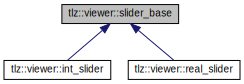
\includegraphics[width=317pt]{classtlz_1_1viewer_1_1slider__base__inherit__graph}
\end{center}
\end{figure}
\subsection*{Public Attributes}
\begin{DoxyCompactItemize}
\item 
int \hyperlink{classtlz_1_1viewer_1_1slider__base_a4146a1545ccb324f95bb5f8108ffabb1}{raw\+\_\+value}
\end{DoxyCompactItemize}
\subsection*{Protected Member Functions}
\begin{DoxyCompactItemize}
\item 
\hyperlink{classtlz_1_1viewer_1_1slider__base_af45c365f5b1c247e79bffcd581df2dad}{slider\+\_\+base} ()=default
\item 
\hyperlink{classtlz_1_1viewer_1_1slider__base_a27c9945842f6d42220b271eb7daed684}{slider\+\_\+base} (const \hyperlink{classtlz_1_1viewer_1_1slider__base}{slider\+\_\+base} \&)=delete
\item 
\hyperlink{classtlz_1_1viewer_1_1slider__base_a6f8b8ab0f6eb764f6b0a66807022a3cc}{slider\+\_\+base} (\hyperlink{classtlz_1_1viewer_1_1slider__base}{slider\+\_\+base} \&\&)=delete
\item 
\hyperlink{classtlz_1_1viewer_1_1slider__base}{slider\+\_\+base} \& \hyperlink{classtlz_1_1viewer_1_1slider__base_a854796a1162271f54f308b04f5343acb}{operator=} (const \hyperlink{classtlz_1_1viewer_1_1slider__base}{slider\+\_\+base} \&)=delete
\item 
\hyperlink{classtlz_1_1viewer_1_1slider__base}{slider\+\_\+base} \& \hyperlink{classtlz_1_1viewer_1_1slider__base_a5d8a1911316e1208cdc01de058eef102}{operator=} (\hyperlink{classtlz_1_1viewer_1_1slider__base}{slider\+\_\+base} \&\&)=delete
\end{DoxyCompactItemize}


\subsection{Detailed Description}


Definition at line 99 of file viewer.\+h.



\subsection{Constructor \& Destructor Documentation}
\index{tlz\+::viewer\+::slider\+\_\+base@{tlz\+::viewer\+::slider\+\_\+base}!slider\+\_\+base@{slider\+\_\+base}}
\index{slider\+\_\+base@{slider\+\_\+base}!tlz\+::viewer\+::slider\+\_\+base@{tlz\+::viewer\+::slider\+\_\+base}}
\subsubsection[{\texorpdfstring{slider\+\_\+base()=default}{slider_base()=default}}]{\setlength{\rightskip}{0pt plus 5cm}tlz\+::viewer\+::slider\+\_\+base\+::slider\+\_\+base (
\begin{DoxyParamCaption}
{}
\end{DoxyParamCaption}
)\hspace{0.3cm}{\ttfamily [protected]}, {\ttfamily [default]}}\hypertarget{classtlz_1_1viewer_1_1slider__base_af45c365f5b1c247e79bffcd581df2dad}{}\label{classtlz_1_1viewer_1_1slider__base_af45c365f5b1c247e79bffcd581df2dad}
\index{tlz\+::viewer\+::slider\+\_\+base@{tlz\+::viewer\+::slider\+\_\+base}!slider\+\_\+base@{slider\+\_\+base}}
\index{slider\+\_\+base@{slider\+\_\+base}!tlz\+::viewer\+::slider\+\_\+base@{tlz\+::viewer\+::slider\+\_\+base}}
\subsubsection[{\texorpdfstring{slider\+\_\+base(const slider\+\_\+base \&)=delete}{slider_base(const slider_base &)=delete}}]{\setlength{\rightskip}{0pt plus 5cm}tlz\+::viewer\+::slider\+\_\+base\+::slider\+\_\+base (
\begin{DoxyParamCaption}
\item[{const {\bf slider\+\_\+base} \&}]{}
\end{DoxyParamCaption}
)\hspace{0.3cm}{\ttfamily [protected]}, {\ttfamily [delete]}}\hypertarget{classtlz_1_1viewer_1_1slider__base_a27c9945842f6d42220b271eb7daed684}{}\label{classtlz_1_1viewer_1_1slider__base_a27c9945842f6d42220b271eb7daed684}
\index{tlz\+::viewer\+::slider\+\_\+base@{tlz\+::viewer\+::slider\+\_\+base}!slider\+\_\+base@{slider\+\_\+base}}
\index{slider\+\_\+base@{slider\+\_\+base}!tlz\+::viewer\+::slider\+\_\+base@{tlz\+::viewer\+::slider\+\_\+base}}
\subsubsection[{\texorpdfstring{slider\+\_\+base(slider\+\_\+base \&\&)=delete}{slider_base(slider_base &&)=delete}}]{\setlength{\rightskip}{0pt plus 5cm}tlz\+::viewer\+::slider\+\_\+base\+::slider\+\_\+base (
\begin{DoxyParamCaption}
\item[{{\bf slider\+\_\+base} \&\&}]{}
\end{DoxyParamCaption}
)\hspace{0.3cm}{\ttfamily [protected]}, {\ttfamily [delete]}}\hypertarget{classtlz_1_1viewer_1_1slider__base_a6f8b8ab0f6eb764f6b0a66807022a3cc}{}\label{classtlz_1_1viewer_1_1slider__base_a6f8b8ab0f6eb764f6b0a66807022a3cc}


\subsection{Member Function Documentation}
\index{tlz\+::viewer\+::slider\+\_\+base@{tlz\+::viewer\+::slider\+\_\+base}!operator=@{operator=}}
\index{operator=@{operator=}!tlz\+::viewer\+::slider\+\_\+base@{tlz\+::viewer\+::slider\+\_\+base}}
\subsubsection[{\texorpdfstring{operator=(const slider\+\_\+base \&)=delete}{operator=(const slider_base &)=delete}}]{\setlength{\rightskip}{0pt plus 5cm}{\bf slider\+\_\+base}\& tlz\+::viewer\+::slider\+\_\+base\+::operator= (
\begin{DoxyParamCaption}
\item[{const {\bf slider\+\_\+base} \&}]{}
\end{DoxyParamCaption}
)\hspace{0.3cm}{\ttfamily [protected]}, {\ttfamily [delete]}}\hypertarget{classtlz_1_1viewer_1_1slider__base_a854796a1162271f54f308b04f5343acb}{}\label{classtlz_1_1viewer_1_1slider__base_a854796a1162271f54f308b04f5343acb}
\index{tlz\+::viewer\+::slider\+\_\+base@{tlz\+::viewer\+::slider\+\_\+base}!operator=@{operator=}}
\index{operator=@{operator=}!tlz\+::viewer\+::slider\+\_\+base@{tlz\+::viewer\+::slider\+\_\+base}}
\subsubsection[{\texorpdfstring{operator=(slider\+\_\+base \&\&)=delete}{operator=(slider_base &&)=delete}}]{\setlength{\rightskip}{0pt plus 5cm}{\bf slider\+\_\+base}\& tlz\+::viewer\+::slider\+\_\+base\+::operator= (
\begin{DoxyParamCaption}
\item[{{\bf slider\+\_\+base} \&\&}]{}
\end{DoxyParamCaption}
)\hspace{0.3cm}{\ttfamily [protected]}, {\ttfamily [delete]}}\hypertarget{classtlz_1_1viewer_1_1slider__base_a5d8a1911316e1208cdc01de058eef102}{}\label{classtlz_1_1viewer_1_1slider__base_a5d8a1911316e1208cdc01de058eef102}


\subsection{Member Data Documentation}
\index{tlz\+::viewer\+::slider\+\_\+base@{tlz\+::viewer\+::slider\+\_\+base}!raw\+\_\+value@{raw\+\_\+value}}
\index{raw\+\_\+value@{raw\+\_\+value}!tlz\+::viewer\+::slider\+\_\+base@{tlz\+::viewer\+::slider\+\_\+base}}
\subsubsection[{\texorpdfstring{raw\+\_\+value}{raw_value}}]{\setlength{\rightskip}{0pt plus 5cm}int tlz\+::viewer\+::slider\+\_\+base\+::raw\+\_\+value}\hypertarget{classtlz_1_1viewer_1_1slider__base_a4146a1545ccb324f95bb5f8108ffabb1}{}\label{classtlz_1_1viewer_1_1slider__base_a4146a1545ccb324f95bb5f8108ffabb1}


Definition at line 101 of file viewer.\+h.



The documentation for this class was generated from the following file\+:\begin{DoxyCompactItemize}
\item 
src/lib/\hyperlink{viewer_8h}{viewer.\+h}\end{DoxyCompactItemize}

\hypertarget{structtlz_1_1straight__depth}{}\section{tlz\+:\+:straight\+\_\+depth Struct Reference}
\label{structtlz_1_1straight__depth}\index{tlz\+::straight\+\_\+depth@{tlz\+::straight\+\_\+depth}}


{\ttfamily \#include $<$straight\+\_\+depths.\+h$>$}

\subsection*{Public Member Functions}
\begin{DoxyCompactItemize}
\item 
\hyperlink{structtlz_1_1straight__depth_a8d35a0d4322e3b81dcd56b0920f136a2}{straight\+\_\+depth} (\hyperlink{namespacetlz_a15fd37cce97f2b8b606af18c2615f602}{real} d=N\+AN, \hyperlink{namespacetlz_a15fd37cce97f2b8b606af18c2615f602}{real} conf=1.\+0)
\item 
\hyperlink{structtlz_1_1straight__depth_a110a722d4afad0b37f11d9dc27b449f1}{operator real} () const 
\end{DoxyCompactItemize}
\subsection*{Public Attributes}
\begin{DoxyCompactItemize}
\item 
\hyperlink{namespacetlz_a15fd37cce97f2b8b606af18c2615f602}{real} \hyperlink{structtlz_1_1straight__depth_a7f8f491d5607692e32111b7f6a57b01f}{depth}
\item 
\hyperlink{namespacetlz_a15fd37cce97f2b8b606af18c2615f602}{real} \hyperlink{structtlz_1_1straight__depth_a4ba5f192be0e4ca1563c1f6c615ea406}{confidence}
\end{DoxyCompactItemize}


\subsection{Detailed Description}


Definition at line 10 of file straight\+\_\+depths.\+h.



\subsection{Constructor \& Destructor Documentation}
\index{tlz\+::straight\+\_\+depth@{tlz\+::straight\+\_\+depth}!straight\+\_\+depth@{straight\+\_\+depth}}
\index{straight\+\_\+depth@{straight\+\_\+depth}!tlz\+::straight\+\_\+depth@{tlz\+::straight\+\_\+depth}}
\subsubsection[{\texorpdfstring{straight\+\_\+depth(real d=\+N\+A\+N, real conf=1.\+0)}{straight_depth(real d=NAN, real conf=1.0)}}]{\setlength{\rightskip}{0pt plus 5cm}tlz\+::straight\+\_\+depth\+::straight\+\_\+depth (
\begin{DoxyParamCaption}
\item[{{\bf real}}]{d = {\ttfamily NAN}, }
\item[{{\bf real}}]{conf = {\ttfamily 1.0}}
\end{DoxyParamCaption}
)\hspace{0.3cm}{\ttfamily [inline]}}\hypertarget{structtlz_1_1straight__depth_a8d35a0d4322e3b81dcd56b0920f136a2}{}\label{structtlz_1_1straight__depth_a8d35a0d4322e3b81dcd56b0920f136a2}


Definition at line 14 of file straight\+\_\+depths.\+h.



\subsection{Member Function Documentation}
\index{tlz\+::straight\+\_\+depth@{tlz\+::straight\+\_\+depth}!operator real@{operator real}}
\index{operator real@{operator real}!tlz\+::straight\+\_\+depth@{tlz\+::straight\+\_\+depth}}
\subsubsection[{\texorpdfstring{operator real() const }{operator real() const }}]{\setlength{\rightskip}{0pt plus 5cm}tlz\+::straight\+\_\+depth\+::operator {\bf real} (
\begin{DoxyParamCaption}
{}
\end{DoxyParamCaption}
) const\hspace{0.3cm}{\ttfamily [inline]}}\hypertarget{structtlz_1_1straight__depth_a110a722d4afad0b37f11d9dc27b449f1}{}\label{structtlz_1_1straight__depth_a110a722d4afad0b37f11d9dc27b449f1}


Definition at line 15 of file straight\+\_\+depths.\+h.



\subsection{Member Data Documentation}
\index{tlz\+::straight\+\_\+depth@{tlz\+::straight\+\_\+depth}!confidence@{confidence}}
\index{confidence@{confidence}!tlz\+::straight\+\_\+depth@{tlz\+::straight\+\_\+depth}}
\subsubsection[{\texorpdfstring{confidence}{confidence}}]{\setlength{\rightskip}{0pt plus 5cm}{\bf real} tlz\+::straight\+\_\+depth\+::confidence}\hypertarget{structtlz_1_1straight__depth_a4ba5f192be0e4ca1563c1f6c615ea406}{}\label{structtlz_1_1straight__depth_a4ba5f192be0e4ca1563c1f6c615ea406}


Definition at line 12 of file straight\+\_\+depths.\+h.

\index{tlz\+::straight\+\_\+depth@{tlz\+::straight\+\_\+depth}!depth@{depth}}
\index{depth@{depth}!tlz\+::straight\+\_\+depth@{tlz\+::straight\+\_\+depth}}
\subsubsection[{\texorpdfstring{depth}{depth}}]{\setlength{\rightskip}{0pt plus 5cm}{\bf real} tlz\+::straight\+\_\+depth\+::depth}\hypertarget{structtlz_1_1straight__depth_a7f8f491d5607692e32111b7f6a57b01f}{}\label{structtlz_1_1straight__depth_a7f8f491d5607692e32111b7f6a57b01f}


Definition at line 11 of file straight\+\_\+depths.\+h.



The documentation for this struct was generated from the following file\+:\begin{DoxyCompactItemize}
\item 
src/calibration/lib/cg/\hyperlink{straight__depths_8h}{straight\+\_\+depths.\+h}\end{DoxyCompactItemize}

\hypertarget{structtarget__camera__position__result}{}\section{target\+\_\+camera\+\_\+position\+\_\+result Struct Reference}
\label{structtarget__camera__position__result}\index{target\+\_\+camera\+\_\+position\+\_\+result@{target\+\_\+camera\+\_\+position\+\_\+result}}
\subsection*{Public Member Functions}
\begin{DoxyCompactItemize}
\item 
\hyperlink{structtarget__camera__position__result_af3a7af786df9768f6c6eed9397255139}{target\+\_\+camera\+\_\+position\+\_\+result} ()=default
\item 
\hyperlink{structtarget__camera__position__result_a2bef2bba908a455f291d42e4a0e04378}{target\+\_\+camera\+\_\+position\+\_\+result} (const \hyperlink{namespacetlz_ae192989bfbe6c700ac84d2a8cf05ebb4}{vec2} \&pos, \hyperlink{namespacetlz_a15fd37cce97f2b8b606af18c2615f602}{real} var)
\item 
\hyperlink{structtarget__camera__position__result_a521a889c20871ab64c9fa053e436019f}{operator bool} () const 
\end{DoxyCompactItemize}
\subsection*{Public Attributes}
\begin{DoxyCompactItemize}
\item 
\hyperlink{namespacetlz_ae192989bfbe6c700ac84d2a8cf05ebb4}{vec2} \hyperlink{structtarget__camera__position__result_aa0097781d0b7c043fb89d697d7659238}{position} = \hyperlink{namespacetlz_ae192989bfbe6c700ac84d2a8cf05ebb4}{vec2}(0.\+0, 0.\+0)
\item 
\hyperlink{namespacetlz_a15fd37cce97f2b8b606af18c2615f602}{real} \hyperlink{structtarget__camera__position__result_af17c7e224cdb90691847e995535c0d50}{variance} = N\+AN
\end{DoxyCompactItemize}


\subsection{Detailed Description}


Definition at line 33 of file cg\+\_\+rcpos\+\_\+from\+\_\+cors.\+cc.



\subsection{Constructor \& Destructor Documentation}
\index{target\+\_\+camera\+\_\+position\+\_\+result@{target\+\_\+camera\+\_\+position\+\_\+result}!target\+\_\+camera\+\_\+position\+\_\+result@{target\+\_\+camera\+\_\+position\+\_\+result}}
\index{target\+\_\+camera\+\_\+position\+\_\+result@{target\+\_\+camera\+\_\+position\+\_\+result}!target\+\_\+camera\+\_\+position\+\_\+result@{target\+\_\+camera\+\_\+position\+\_\+result}}
\subsubsection[{\texorpdfstring{target\+\_\+camera\+\_\+position\+\_\+result()=default}{target_camera_position_result()=default}}]{\setlength{\rightskip}{0pt plus 5cm}target\+\_\+camera\+\_\+position\+\_\+result\+::target\+\_\+camera\+\_\+position\+\_\+result (
\begin{DoxyParamCaption}
{}
\end{DoxyParamCaption}
)\hspace{0.3cm}{\ttfamily [default]}}\hypertarget{structtarget__camera__position__result_af3a7af786df9768f6c6eed9397255139}{}\label{structtarget__camera__position__result_af3a7af786df9768f6c6eed9397255139}
\index{target\+\_\+camera\+\_\+position\+\_\+result@{target\+\_\+camera\+\_\+position\+\_\+result}!target\+\_\+camera\+\_\+position\+\_\+result@{target\+\_\+camera\+\_\+position\+\_\+result}}
\index{target\+\_\+camera\+\_\+position\+\_\+result@{target\+\_\+camera\+\_\+position\+\_\+result}!target\+\_\+camera\+\_\+position\+\_\+result@{target\+\_\+camera\+\_\+position\+\_\+result}}
\subsubsection[{\texorpdfstring{target\+\_\+camera\+\_\+position\+\_\+result(const vec2 \&pos, real var)}{target_camera_position_result(const vec2 &pos, real var)}}]{\setlength{\rightskip}{0pt plus 5cm}target\+\_\+camera\+\_\+position\+\_\+result\+::target\+\_\+camera\+\_\+position\+\_\+result (
\begin{DoxyParamCaption}
\item[{const {\bf vec2} \&}]{pos, }
\item[{{\bf real}}]{var}
\end{DoxyParamCaption}
)\hspace{0.3cm}{\ttfamily [inline]}}\hypertarget{structtarget__camera__position__result_a2bef2bba908a455f291d42e4a0e04378}{}\label{structtarget__camera__position__result_a2bef2bba908a455f291d42e4a0e04378}


Definition at line 38 of file cg\+\_\+rcpos\+\_\+from\+\_\+cors.\+cc.



\subsection{Member Function Documentation}
\index{target\+\_\+camera\+\_\+position\+\_\+result@{target\+\_\+camera\+\_\+position\+\_\+result}!operator bool@{operator bool}}
\index{operator bool@{operator bool}!target\+\_\+camera\+\_\+position\+\_\+result@{target\+\_\+camera\+\_\+position\+\_\+result}}
\subsubsection[{\texorpdfstring{operator bool() const }{operator bool() const }}]{\setlength{\rightskip}{0pt plus 5cm}target\+\_\+camera\+\_\+position\+\_\+result\+::operator bool (
\begin{DoxyParamCaption}
{}
\end{DoxyParamCaption}
) const\hspace{0.3cm}{\ttfamily [inline]}, {\ttfamily [explicit]}}\hypertarget{structtarget__camera__position__result_a521a889c20871ab64c9fa053e436019f}{}\label{structtarget__camera__position__result_a521a889c20871ab64c9fa053e436019f}


Definition at line 41 of file cg\+\_\+rcpos\+\_\+from\+\_\+cors.\+cc.



\subsection{Member Data Documentation}
\index{target\+\_\+camera\+\_\+position\+\_\+result@{target\+\_\+camera\+\_\+position\+\_\+result}!position@{position}}
\index{position@{position}!target\+\_\+camera\+\_\+position\+\_\+result@{target\+\_\+camera\+\_\+position\+\_\+result}}
\subsubsection[{\texorpdfstring{position}{position}}]{\setlength{\rightskip}{0pt plus 5cm}{\bf vec2} target\+\_\+camera\+\_\+position\+\_\+result\+::position = {\bf vec2}(0.\+0, 0.\+0)}\hypertarget{structtarget__camera__position__result_aa0097781d0b7c043fb89d697d7659238}{}\label{structtarget__camera__position__result_aa0097781d0b7c043fb89d697d7659238}


Definition at line 34 of file cg\+\_\+rcpos\+\_\+from\+\_\+cors.\+cc.

\index{target\+\_\+camera\+\_\+position\+\_\+result@{target\+\_\+camera\+\_\+position\+\_\+result}!variance@{variance}}
\index{variance@{variance}!target\+\_\+camera\+\_\+position\+\_\+result@{target\+\_\+camera\+\_\+position\+\_\+result}}
\subsubsection[{\texorpdfstring{variance}{variance}}]{\setlength{\rightskip}{0pt plus 5cm}{\bf real} target\+\_\+camera\+\_\+position\+\_\+result\+::variance = N\+AN}\hypertarget{structtarget__camera__position__result_af17c7e224cdb90691847e995535c0d50}{}\label{structtarget__camera__position__result_af17c7e224cdb90691847e995535c0d50}


Definition at line 35 of file cg\+\_\+rcpos\+\_\+from\+\_\+cors.\+cc.



The documentation for this struct was generated from the following file\+:\begin{DoxyCompactItemize}
\item 
src/calibration/\hyperlink{cg__rcpos__from__cors_8cc}{cg\+\_\+rcpos\+\_\+from\+\_\+cors.\+cc}\end{DoxyCompactItemize}

\hypertarget{classpylib_1_1temporary_1_1temporary__file}{}\section{pylib.\+temporary.\+temporary\+\_\+file Class Reference}
\label{classpylib_1_1temporary_1_1temporary__file}\index{pylib.\+temporary.\+temporary\+\_\+file@{pylib.\+temporary.\+temporary\+\_\+file}}


Inheritance diagram for pylib.\+temporary.\+temporary\+\_\+file\+:
\nopagebreak
\begin{figure}[H]
\begin{center}
\leavevmode
\includegraphics[width=350pt]{classpylib_1_1temporary_1_1temporary__file__inherit__graph}
\end{center}
\end{figure}


Collaboration diagram for pylib.\+temporary.\+temporary\+\_\+file\+:
\nopagebreak
\begin{figure}[H]
\begin{center}
\leavevmode
\includegraphics[width=228pt]{classpylib_1_1temporary_1_1temporary__file__coll__graph}
\end{center}
\end{figure}
\subsection*{Public Member Functions}
\begin{DoxyCompactItemize}
\item 
def \hyperlink{classpylib_1_1temporary_1_1temporary__file_a2fa7c4673cadc067ade6f5a62e73bbfe}{\+\_\+\+\_\+init\+\_\+\+\_\+} (self, ext)
\item 
def \hyperlink{classpylib_1_1temporary_1_1temporary__file_af8cc5acb89454c03b51f9918fa3aa069}{\+\_\+\+\_\+enter\+\_\+\+\_\+} (self)
\item 
def \hyperlink{classpylib_1_1temporary_1_1temporary__file_afd2465f566361a8b2bba1a2943023704}{\+\_\+\+\_\+exit\+\_\+\+\_\+} (self, exc\+\_\+type, exc\+\_\+value, traceback)
\item 
def \hyperlink{classpylib_1_1temporary_1_1temporary__file_a198ec454a96e1dd392bc3eaa99ee0a8c}{write\+\_\+file} (self, f)
\end{DoxyCompactItemize}
\subsection*{Static Public Attributes}
\begin{DoxyCompactItemize}
\item 
\hyperlink{classpylib_1_1temporary_1_1temporary__file_aed23d05f04833724e81e41d80363a65c}{filename} = None
\item 
\hyperlink{classpylib_1_1temporary_1_1temporary__file_a4662cc55e879791c5931ab72ad40eed3}{extension} = None
\end{DoxyCompactItemize}


\subsection{Detailed Description}


Definition at line 8 of file temporary.\+py.



\subsection{Constructor \& Destructor Documentation}
\index{pylib\+::temporary\+::temporary\+\_\+file@{pylib\+::temporary\+::temporary\+\_\+file}!\+\_\+\+\_\+init\+\_\+\+\_\+@{\+\_\+\+\_\+init\+\_\+\+\_\+}}
\index{\+\_\+\+\_\+init\+\_\+\+\_\+@{\+\_\+\+\_\+init\+\_\+\+\_\+}!pylib\+::temporary\+::temporary\+\_\+file@{pylib\+::temporary\+::temporary\+\_\+file}}
\subsubsection[{\texorpdfstring{\+\_\+\+\_\+init\+\_\+\+\_\+(self, ext)}{__init__(self, ext)}}]{\setlength{\rightskip}{0pt plus 5cm}def pylib.\+temporary.\+temporary\+\_\+file.\+\_\+\+\_\+init\+\_\+\+\_\+ (
\begin{DoxyParamCaption}
\item[{}]{self, }
\item[{}]{ext}
\end{DoxyParamCaption}
)}\hypertarget{classpylib_1_1temporary_1_1temporary__file_a2fa7c4673cadc067ade6f5a62e73bbfe}{}\label{classpylib_1_1temporary_1_1temporary__file_a2fa7c4673cadc067ade6f5a62e73bbfe}


Definition at line 12 of file temporary.\+py.



\subsection{Member Function Documentation}
\index{pylib\+::temporary\+::temporary\+\_\+file@{pylib\+::temporary\+::temporary\+\_\+file}!\+\_\+\+\_\+enter\+\_\+\+\_\+@{\+\_\+\+\_\+enter\+\_\+\+\_\+}}
\index{\+\_\+\+\_\+enter\+\_\+\+\_\+@{\+\_\+\+\_\+enter\+\_\+\+\_\+}!pylib\+::temporary\+::temporary\+\_\+file@{pylib\+::temporary\+::temporary\+\_\+file}}
\subsubsection[{\texorpdfstring{\+\_\+\+\_\+enter\+\_\+\+\_\+(self)}{__enter__(self)}}]{\setlength{\rightskip}{0pt plus 5cm}def pylib.\+temporary.\+temporary\+\_\+file.\+\_\+\+\_\+enter\+\_\+\+\_\+ (
\begin{DoxyParamCaption}
\item[{}]{self}
\end{DoxyParamCaption}
)}\hypertarget{classpylib_1_1temporary_1_1temporary__file_af8cc5acb89454c03b51f9918fa3aa069}{}\label{classpylib_1_1temporary_1_1temporary__file_af8cc5acb89454c03b51f9918fa3aa069}


Definition at line 16 of file temporary.\+py.

\index{pylib\+::temporary\+::temporary\+\_\+file@{pylib\+::temporary\+::temporary\+\_\+file}!\+\_\+\+\_\+exit\+\_\+\+\_\+@{\+\_\+\+\_\+exit\+\_\+\+\_\+}}
\index{\+\_\+\+\_\+exit\+\_\+\+\_\+@{\+\_\+\+\_\+exit\+\_\+\+\_\+}!pylib\+::temporary\+::temporary\+\_\+file@{pylib\+::temporary\+::temporary\+\_\+file}}
\subsubsection[{\texorpdfstring{\+\_\+\+\_\+exit\+\_\+\+\_\+(self, exc\+\_\+type, exc\+\_\+value, traceback)}{__exit__(self, exc_type, exc_value, traceback)}}]{\setlength{\rightskip}{0pt plus 5cm}def pylib.\+temporary.\+temporary\+\_\+file.\+\_\+\+\_\+exit\+\_\+\+\_\+ (
\begin{DoxyParamCaption}
\item[{}]{self, }
\item[{}]{exc\+\_\+type, }
\item[{}]{exc\+\_\+value, }
\item[{}]{traceback}
\end{DoxyParamCaption}
)}\hypertarget{classpylib_1_1temporary_1_1temporary__file_afd2465f566361a8b2bba1a2943023704}{}\label{classpylib_1_1temporary_1_1temporary__file_afd2465f566361a8b2bba1a2943023704}


Definition at line 35 of file temporary.\+py.

\index{pylib\+::temporary\+::temporary\+\_\+file@{pylib\+::temporary\+::temporary\+\_\+file}!write\+\_\+file@{write\+\_\+file}}
\index{write\+\_\+file@{write\+\_\+file}!pylib\+::temporary\+::temporary\+\_\+file@{pylib\+::temporary\+::temporary\+\_\+file}}
\subsubsection[{\texorpdfstring{write\+\_\+file(self, f)}{write_file(self, f)}}]{\setlength{\rightskip}{0pt plus 5cm}def pylib.\+temporary.\+temporary\+\_\+file.\+write\+\_\+file (
\begin{DoxyParamCaption}
\item[{}]{self, }
\item[{}]{f}
\end{DoxyParamCaption}
)}\hypertarget{classpylib_1_1temporary_1_1temporary__file_a198ec454a96e1dd392bc3eaa99ee0a8c}{}\label{classpylib_1_1temporary_1_1temporary__file_a198ec454a96e1dd392bc3eaa99ee0a8c}


Definition at line 45 of file temporary.\+py.



\subsection{Member Data Documentation}
\index{pylib\+::temporary\+::temporary\+\_\+file@{pylib\+::temporary\+::temporary\+\_\+file}!extension@{extension}}
\index{extension@{extension}!pylib\+::temporary\+::temporary\+\_\+file@{pylib\+::temporary\+::temporary\+\_\+file}}
\subsubsection[{\texorpdfstring{extension}{extension}}]{\setlength{\rightskip}{0pt plus 5cm}pylib.\+temporary.\+temporary\+\_\+file.\+extension = None\hspace{0.3cm}{\ttfamily [static]}}\hypertarget{classpylib_1_1temporary_1_1temporary__file_a4662cc55e879791c5931ab72ad40eed3}{}\label{classpylib_1_1temporary_1_1temporary__file_a4662cc55e879791c5931ab72ad40eed3}


Definition at line 10 of file temporary.\+py.

\index{pylib\+::temporary\+::temporary\+\_\+file@{pylib\+::temporary\+::temporary\+\_\+file}!filename@{filename}}
\index{filename@{filename}!pylib\+::temporary\+::temporary\+\_\+file@{pylib\+::temporary\+::temporary\+\_\+file}}
\subsubsection[{\texorpdfstring{filename}{filename}}]{\setlength{\rightskip}{0pt plus 5cm}pylib.\+temporary.\+temporary\+\_\+file.\+filename = None\hspace{0.3cm}{\ttfamily [static]}}\hypertarget{classpylib_1_1temporary_1_1temporary__file_aed23d05f04833724e81e41d80363a65c}{}\label{classpylib_1_1temporary_1_1temporary__file_aed23d05f04833724e81e41d80363a65c}


Definition at line 9 of file temporary.\+py.



The documentation for this class was generated from the following file\+:\begin{DoxyCompactItemize}
\item 
src/lib/pylib/\hyperlink{temporary_8py}{temporary.\+py}\end{DoxyCompactItemize}

\hypertarget{classpylib_1_1temporary_1_1temporary__in__json}{}\section{pylib.\+temporary.\+temporary\+\_\+in\+\_\+json Class Reference}
\label{classpylib_1_1temporary_1_1temporary__in__json}\index{pylib.\+temporary.\+temporary\+\_\+in\+\_\+json@{pylib.\+temporary.\+temporary\+\_\+in\+\_\+json}}


Inheritance diagram for pylib.\+temporary.\+temporary\+\_\+in\+\_\+json\+:
\nopagebreak
\begin{figure}[H]
\begin{center}
\leavevmode
\includegraphics[width=228pt]{classpylib_1_1temporary_1_1temporary__in__json__inherit__graph}
\end{center}
\end{figure}


Collaboration diagram for pylib.\+temporary.\+temporary\+\_\+in\+\_\+json\+:
\nopagebreak
\begin{figure}[H]
\begin{center}
\leavevmode
\includegraphics[width=228pt]{classpylib_1_1temporary_1_1temporary__in__json__coll__graph}
\end{center}
\end{figure}
\subsection*{Public Member Functions}
\begin{DoxyCompactItemize}
\item 
def \hyperlink{classpylib_1_1temporary_1_1temporary__in__json_a949124b08a48fe601cbf8eea0b09783e}{\+\_\+\+\_\+init\+\_\+\+\_\+} (self, j)
\item 
def \hyperlink{classpylib_1_1temporary_1_1temporary__in__json_a97e280e7f7817fc090e622d2c63d3426}{write\+\_\+file} (self, f)
\end{DoxyCompactItemize}
\subsection*{Static Public Attributes}
\begin{DoxyCompactItemize}
\item 
\hyperlink{classpylib_1_1temporary_1_1temporary__in__json_a2b87f0ff9fcd462736de3cc49b98d6bf}{json} = None
\end{DoxyCompactItemize}


\subsection{Detailed Description}


Definition at line 49 of file temporary.\+py.



\subsection{Constructor \& Destructor Documentation}
\index{pylib\+::temporary\+::temporary\+\_\+in\+\_\+json@{pylib\+::temporary\+::temporary\+\_\+in\+\_\+json}!\+\_\+\+\_\+init\+\_\+\+\_\+@{\+\_\+\+\_\+init\+\_\+\+\_\+}}
\index{\+\_\+\+\_\+init\+\_\+\+\_\+@{\+\_\+\+\_\+init\+\_\+\+\_\+}!pylib\+::temporary\+::temporary\+\_\+in\+\_\+json@{pylib\+::temporary\+::temporary\+\_\+in\+\_\+json}}
\subsubsection[{\texorpdfstring{\+\_\+\+\_\+init\+\_\+\+\_\+(self, j)}{__init__(self, j)}}]{\setlength{\rightskip}{0pt plus 5cm}def pylib.\+temporary.\+temporary\+\_\+in\+\_\+json.\+\_\+\+\_\+init\+\_\+\+\_\+ (
\begin{DoxyParamCaption}
\item[{}]{self, }
\item[{}]{j}
\end{DoxyParamCaption}
)}\hypertarget{classpylib_1_1temporary_1_1temporary__in__json_a949124b08a48fe601cbf8eea0b09783e}{}\label{classpylib_1_1temporary_1_1temporary__in__json_a949124b08a48fe601cbf8eea0b09783e}


Definition at line 52 of file temporary.\+py.



\subsection{Member Function Documentation}
\index{pylib\+::temporary\+::temporary\+\_\+in\+\_\+json@{pylib\+::temporary\+::temporary\+\_\+in\+\_\+json}!write\+\_\+file@{write\+\_\+file}}
\index{write\+\_\+file@{write\+\_\+file}!pylib\+::temporary\+::temporary\+\_\+in\+\_\+json@{pylib\+::temporary\+::temporary\+\_\+in\+\_\+json}}
\subsubsection[{\texorpdfstring{write\+\_\+file(self, f)}{write_file(self, f)}}]{\setlength{\rightskip}{0pt plus 5cm}def pylib.\+temporary.\+temporary\+\_\+in\+\_\+json.\+write\+\_\+file (
\begin{DoxyParamCaption}
\item[{}]{self, }
\item[{}]{f}
\end{DoxyParamCaption}
)}\hypertarget{classpylib_1_1temporary_1_1temporary__in__json_a97e280e7f7817fc090e622d2c63d3426}{}\label{classpylib_1_1temporary_1_1temporary__in__json_a97e280e7f7817fc090e622d2c63d3426}


Definition at line 56 of file temporary.\+py.



\subsection{Member Data Documentation}
\index{pylib\+::temporary\+::temporary\+\_\+in\+\_\+json@{pylib\+::temporary\+::temporary\+\_\+in\+\_\+json}!json@{json}}
\index{json@{json}!pylib\+::temporary\+::temporary\+\_\+in\+\_\+json@{pylib\+::temporary\+::temporary\+\_\+in\+\_\+json}}
\subsubsection[{\texorpdfstring{json}{json}}]{\setlength{\rightskip}{0pt plus 5cm}pylib.\+temporary.\+temporary\+\_\+in\+\_\+json.\+json = None\hspace{0.3cm}{\ttfamily [static]}}\hypertarget{classpylib_1_1temporary_1_1temporary__in__json_a2b87f0ff9fcd462736de3cc49b98d6bf}{}\label{classpylib_1_1temporary_1_1temporary__in__json_a2b87f0ff9fcd462736de3cc49b98d6bf}


Definition at line 50 of file temporary.\+py.



The documentation for this class was generated from the following file\+:\begin{DoxyCompactItemize}
\item 
src/lib/pylib/\hyperlink{temporary_8py}{temporary.\+py}\end{DoxyCompactItemize}

\hypertarget{classpylib_1_1temporary_1_1temporary__out__json}{}\section{pylib.\+temporary.\+temporary\+\_\+out\+\_\+json Class Reference}
\label{classpylib_1_1temporary_1_1temporary__out__json}\index{pylib.\+temporary.\+temporary\+\_\+out\+\_\+json@{pylib.\+temporary.\+temporary\+\_\+out\+\_\+json}}


Inheritance diagram for pylib.\+temporary.\+temporary\+\_\+out\+\_\+json\+:
\nopagebreak
\begin{figure}[H]
\begin{center}
\leavevmode
\includegraphics[width=228pt]{classpylib_1_1temporary_1_1temporary__out__json__inherit__graph}
\end{center}
\end{figure}


Collaboration diagram for pylib.\+temporary.\+temporary\+\_\+out\+\_\+json\+:
\nopagebreak
\begin{figure}[H]
\begin{center}
\leavevmode
\includegraphics[width=228pt]{classpylib_1_1temporary_1_1temporary__out__json__coll__graph}
\end{center}
\end{figure}
\subsection*{Public Member Functions}
\begin{DoxyCompactItemize}
\item 
def \hyperlink{classpylib_1_1temporary_1_1temporary__out__json_aced24965f73822dc12a92747c6528a52}{\+\_\+\+\_\+init\+\_\+\+\_\+} (self)
\item 
def \hyperlink{classpylib_1_1temporary_1_1temporary__out__json_a58991e5e90a8b7d29ac7c1e222f21dc7}{json} (self)
\end{DoxyCompactItemize}
\subsection*{Additional Inherited Members}


\subsection{Detailed Description}


Definition at line 60 of file temporary.\+py.



\subsection{Constructor \& Destructor Documentation}
\index{pylib\+::temporary\+::temporary\+\_\+out\+\_\+json@{pylib\+::temporary\+::temporary\+\_\+out\+\_\+json}!\+\_\+\+\_\+init\+\_\+\+\_\+@{\+\_\+\+\_\+init\+\_\+\+\_\+}}
\index{\+\_\+\+\_\+init\+\_\+\+\_\+@{\+\_\+\+\_\+init\+\_\+\+\_\+}!pylib\+::temporary\+::temporary\+\_\+out\+\_\+json@{pylib\+::temporary\+::temporary\+\_\+out\+\_\+json}}
\subsubsection[{\texorpdfstring{\+\_\+\+\_\+init\+\_\+\+\_\+(self)}{__init__(self)}}]{\setlength{\rightskip}{0pt plus 5cm}def pylib.\+temporary.\+temporary\+\_\+out\+\_\+json.\+\_\+\+\_\+init\+\_\+\+\_\+ (
\begin{DoxyParamCaption}
\item[{}]{self}
\end{DoxyParamCaption}
)}\hypertarget{classpylib_1_1temporary_1_1temporary__out__json_aced24965f73822dc12a92747c6528a52}{}\label{classpylib_1_1temporary_1_1temporary__out__json_aced24965f73822dc12a92747c6528a52}


Definition at line 61 of file temporary.\+py.



\subsection{Member Function Documentation}
\index{pylib\+::temporary\+::temporary\+\_\+out\+\_\+json@{pylib\+::temporary\+::temporary\+\_\+out\+\_\+json}!json@{json}}
\index{json@{json}!pylib\+::temporary\+::temporary\+\_\+out\+\_\+json@{pylib\+::temporary\+::temporary\+\_\+out\+\_\+json}}
\subsubsection[{\texorpdfstring{json(self)}{json(self)}}]{\setlength{\rightskip}{0pt plus 5cm}def pylib.\+temporary.\+temporary\+\_\+out\+\_\+json.\+json (
\begin{DoxyParamCaption}
\item[{}]{self}
\end{DoxyParamCaption}
)}\hypertarget{classpylib_1_1temporary_1_1temporary__out__json_a58991e5e90a8b7d29ac7c1e222f21dc7}{}\label{classpylib_1_1temporary_1_1temporary__out__json_a58991e5e90a8b7d29ac7c1e222f21dc7}


Definition at line 64 of file temporary.\+py.



The documentation for this class was generated from the following file\+:\begin{DoxyCompactItemize}
\item 
src/lib/pylib/\hyperlink{temporary_8py}{temporary.\+py}\end{DoxyCompactItemize}

\hypertarget{structtlz_1_1view__homography}{}\section{tlz\+:\+:view\+\_\+homography Struct Reference}
\label{structtlz_1_1view__homography}\index{tlz\+::view\+\_\+homography@{tlz\+::view\+\_\+homography}}


{\ttfamily \#include $<$view\+\_\+homography.\+h$>$}

\subsection*{Public Attributes}
\begin{DoxyCompactItemize}
\item 
\hyperlink{namespacetlz_a6679497d5121f319147594e1f344ef57}{mat33} \hyperlink{structtlz_1_1view__homography_ac1e52bf8cd63adbfb89179c618fbe9d3}{mat}
\item 
\hyperlink{namespacetlz_a15fd37cce97f2b8b606af18c2615f602}{real} \hyperlink{structtlz_1_1view__homography_a03fdc6014f5e21a3d5a86cc7e312b034}{err} = N\+AN
\end{DoxyCompactItemize}


\subsection{Detailed Description}


Definition at line 13 of file view\+\_\+homography.\+h.



\subsection{Member Data Documentation}
\index{tlz\+::view\+\_\+homography@{tlz\+::view\+\_\+homography}!err@{err}}
\index{err@{err}!tlz\+::view\+\_\+homography@{tlz\+::view\+\_\+homography}}
\subsubsection[{\texorpdfstring{err}{err}}]{\setlength{\rightskip}{0pt plus 5cm}{\bf real} tlz\+::view\+\_\+homography\+::err = N\+AN}\hypertarget{structtlz_1_1view__homography_a03fdc6014f5e21a3d5a86cc7e312b034}{}\label{structtlz_1_1view__homography_a03fdc6014f5e21a3d5a86cc7e312b034}


Definition at line 15 of file view\+\_\+homography.\+h.

\index{tlz\+::view\+\_\+homography@{tlz\+::view\+\_\+homography}!mat@{mat}}
\index{mat@{mat}!tlz\+::view\+\_\+homography@{tlz\+::view\+\_\+homography}}
\subsubsection[{\texorpdfstring{mat}{mat}}]{\setlength{\rightskip}{0pt plus 5cm}{\bf mat33} tlz\+::view\+\_\+homography\+::mat}\hypertarget{structtlz_1_1view__homography_ac1e52bf8cd63adbfb89179c618fbe9d3}{}\label{structtlz_1_1view__homography_ac1e52bf8cd63adbfb89179c618fbe9d3}


Definition at line 14 of file view\+\_\+homography.\+h.



The documentation for this struct was generated from the following file\+:\begin{DoxyCompactItemize}
\item 
src/lib/\hyperlink{view__homography_8h}{view\+\_\+homography.\+h}\end{DoxyCompactItemize}

\hypertarget{structtlz_1_1view__index}{}\section{tlz\+:\+:view\+\_\+index Struct Reference}
\label{structtlz_1_1view__index}\index{tlz\+::view\+\_\+index@{tlz\+::view\+\_\+index}}


{\ttfamily \#include $<$common.\+h$>$}



Inheritance diagram for tlz\+:\+:view\+\_\+index\+:
\nopagebreak
\begin{figure}[H]
\begin{center}
\leavevmode
\includegraphics[width=162pt]{structtlz_1_1view__index__inherit__graph}
\end{center}
\end{figure}


Collaboration diagram for tlz\+:\+:view\+\_\+index\+:
\nopagebreak
\begin{figure}[H]
\begin{center}
\leavevmode
\includegraphics[width=162pt]{structtlz_1_1view__index__coll__graph}
\end{center}
\end{figure}
\subsection*{Public Member Functions}
\begin{DoxyCompactItemize}
\item 
bool \hyperlink{structtlz_1_1view__index_a795d2e69452fa9cf92a8bf776bb6e209}{is\+\_\+valid} () const 
\item 
\hyperlink{structtlz_1_1view__index_a8a73d6356ac086bd0faa55a9b5ae2c9f}{operator bool} () const 
\item 
bool \hyperlink{structtlz_1_1view__index_a3ed08e458871f0bd2639ffdb07fdb183}{is\+\_\+1d} () const 
\item 
bool \hyperlink{structtlz_1_1view__index_a20518c30015d833cdb2a69b524886b96}{is\+\_\+2d} () const 
\item 
\hyperlink{structtlz_1_1view__index_aef9246db6f8a0720ec3cd935119bd2cf}{view\+\_\+index} (int x\+\_\+=-\/1, int y\+\_\+=-\/1)
\end{DoxyCompactItemize}
\subsection*{Additional Inherited Members}


\subsection{Detailed Description}


Definition at line 116 of file common.\+h.



\subsection{Constructor \& Destructor Documentation}
\index{tlz\+::view\+\_\+index@{tlz\+::view\+\_\+index}!view\+\_\+index@{view\+\_\+index}}
\index{view\+\_\+index@{view\+\_\+index}!tlz\+::view\+\_\+index@{tlz\+::view\+\_\+index}}
\subsubsection[{\texorpdfstring{view\+\_\+index(int x\+\_\+=-\/1, int y\+\_\+=-\/1)}{view_index(int x_=-1, int y_=-1)}}]{\setlength{\rightskip}{0pt plus 5cm}tlz\+::view\+\_\+index\+::view\+\_\+index (
\begin{DoxyParamCaption}
\item[{int}]{x\+\_\+ = {\ttfamily -\/1}, }
\item[{int}]{y\+\_\+ = {\ttfamily -\/1}}
\end{DoxyParamCaption}
)\hspace{0.3cm}{\ttfamily [inline]}, {\ttfamily [explicit]}}\hypertarget{structtlz_1_1view__index_aef9246db6f8a0720ec3cd935119bd2cf}{}\label{structtlz_1_1view__index_aef9246db6f8a0720ec3cd935119bd2cf}


Definition at line 123 of file common.\+h.



\subsection{Member Function Documentation}
\index{tlz\+::view\+\_\+index@{tlz\+::view\+\_\+index}!is\+\_\+1d@{is\+\_\+1d}}
\index{is\+\_\+1d@{is\+\_\+1d}!tlz\+::view\+\_\+index@{tlz\+::view\+\_\+index}}
\subsubsection[{\texorpdfstring{is\+\_\+1d() const }{is_1d() const }}]{\setlength{\rightskip}{0pt plus 5cm}bool tlz\+::view\+\_\+index\+::is\+\_\+1d (
\begin{DoxyParamCaption}
{}
\end{DoxyParamCaption}
) const\hspace{0.3cm}{\ttfamily [inline]}}\hypertarget{structtlz_1_1view__index_a3ed08e458871f0bd2639ffdb07fdb183}{}\label{structtlz_1_1view__index_a3ed08e458871f0bd2639ffdb07fdb183}


Definition at line 120 of file common.\+h.

\index{tlz\+::view\+\_\+index@{tlz\+::view\+\_\+index}!is\+\_\+2d@{is\+\_\+2d}}
\index{is\+\_\+2d@{is\+\_\+2d}!tlz\+::view\+\_\+index@{tlz\+::view\+\_\+index}}
\subsubsection[{\texorpdfstring{is\+\_\+2d() const }{is_2d() const }}]{\setlength{\rightskip}{0pt plus 5cm}bool tlz\+::view\+\_\+index\+::is\+\_\+2d (
\begin{DoxyParamCaption}
{}
\end{DoxyParamCaption}
) const\hspace{0.3cm}{\ttfamily [inline]}}\hypertarget{structtlz_1_1view__index_a20518c30015d833cdb2a69b524886b96}{}\label{structtlz_1_1view__index_a20518c30015d833cdb2a69b524886b96}


Definition at line 121 of file common.\+h.

\index{tlz\+::view\+\_\+index@{tlz\+::view\+\_\+index}!is\+\_\+valid@{is\+\_\+valid}}
\index{is\+\_\+valid@{is\+\_\+valid}!tlz\+::view\+\_\+index@{tlz\+::view\+\_\+index}}
\subsubsection[{\texorpdfstring{is\+\_\+valid() const }{is_valid() const }}]{\setlength{\rightskip}{0pt plus 5cm}bool tlz\+::view\+\_\+index\+::is\+\_\+valid (
\begin{DoxyParamCaption}
{}
\end{DoxyParamCaption}
) const\hspace{0.3cm}{\ttfamily [inline]}}\hypertarget{structtlz_1_1view__index_a795d2e69452fa9cf92a8bf776bb6e209}{}\label{structtlz_1_1view__index_a795d2e69452fa9cf92a8bf776bb6e209}


Definition at line 117 of file common.\+h.

\index{tlz\+::view\+\_\+index@{tlz\+::view\+\_\+index}!operator bool@{operator bool}}
\index{operator bool@{operator bool}!tlz\+::view\+\_\+index@{tlz\+::view\+\_\+index}}
\subsubsection[{\texorpdfstring{operator bool() const }{operator bool() const }}]{\setlength{\rightskip}{0pt plus 5cm}tlz\+::view\+\_\+index\+::operator bool (
\begin{DoxyParamCaption}
{}
\end{DoxyParamCaption}
) const\hspace{0.3cm}{\ttfamily [inline]}, {\ttfamily [explicit]}}\hypertarget{structtlz_1_1view__index_a8a73d6356ac086bd0faa55a9b5ae2c9f}{}\label{structtlz_1_1view__index_a8a73d6356ac086bd0faa55a9b5ae2c9f}


Definition at line 118 of file common.\+h.



The documentation for this struct was generated from the following file\+:\begin{DoxyCompactItemize}
\item 
src/lib/\hyperlink{lib_2common_8h}{common.\+h}\end{DoxyCompactItemize}

\hypertarget{classtlz_1_1viewer}{}\section{tlz\+:\+:viewer Class Reference}
\label{classtlz_1_1viewer}\index{tlz\+::viewer@{tlz\+::viewer}}


{\ttfamily \#include $<$viewer.\+h$>$}

\subsection*{Classes}
\begin{DoxyCompactItemize}
\item 
class \hyperlink{classtlz_1_1viewer_1_1int__slider}{int\+\_\+slider}
\item 
class \hyperlink{classtlz_1_1viewer_1_1real__slider}{real\+\_\+slider}
\item 
class \hyperlink{classtlz_1_1viewer_1_1slider__base}{slider\+\_\+base}
\end{DoxyCompactItemize}
\subsection*{Public Types}
\begin{DoxyCompactItemize}
\item 
enum \hyperlink{classtlz_1_1viewer_a280addd8c203232bdaf5ae4dc85a139a}{text\+\_\+alignment} \{ \hyperlink{classtlz_1_1viewer_a280addd8c203232bdaf5ae4dc85a139aa7d9efcc435fbfbde49c6c8e256405f68}{left}, 
\hyperlink{classtlz_1_1viewer_a280addd8c203232bdaf5ae4dc85a139aa896ad3baba90240ef5aa5c2c66b14fcf}{center}, 
\hyperlink{classtlz_1_1viewer_a280addd8c203232bdaf5ae4dc85a139aa242c9b07c716c6be5cade53a54244ec3}{right}
 \}
\end{DoxyCompactItemize}
\subsection*{Public Member Functions}
\begin{DoxyCompactItemize}
\item 
\hyperlink{classtlz_1_1viewer_ab840cedc6c257c4270c43d59705842cc}{viewer} (const std\+::string \&title, int \hyperlink{classtlz_1_1viewer_acc43bf1dd1d0c3cdc35a948d4c194769}{width}, int \hyperlink{classtlz_1_1viewer_af74a8aef9dde68eeff6b1e2561b39014}{height}, bool resizeable=false)
\item 
\hyperlink{classtlz_1_1viewer_a197747fd66bf0c2cb69ac598e08f6e79}{viewer} (const std\+::string \&title, cv\+::\+Size sz, bool resizeable=false)
\item 
\hyperlink{classtlz_1_1viewer_a3d7acc2df49af00c659dd55c6898344d}{viewer} (int \hyperlink{classtlz_1_1viewer_acc43bf1dd1d0c3cdc35a948d4c194769}{width}, int \hyperlink{classtlz_1_1viewer_af74a8aef9dde68eeff6b1e2561b39014}{height}, bool resizeable=false)
\item 
\hyperlink{classtlz_1_1viewer_a29d63e7cbf892927adc12c2c35c28c5d}{viewer} (cv\+::\+Size sz, bool resizeable=false)
\item 
\hyperlink{classtlz_1_1viewer_af946932c9c9ac062feaa9e15b55b79b8}{viewer} (const std\+::string \&title, bool resizeable=false)
\item 
\hyperlink{classtlz_1_1viewer_a916b709d0d5e9f08f0291c104b2edb0b}{viewer} (const \hyperlink{classtlz_1_1viewer}{viewer} \&)=delete
\item 
\hyperlink{classtlz_1_1viewer_a2db3e67ba1350a8be839d1725bd7ebc2}{$\sim$viewer} ()
\item 
\hyperlink{classtlz_1_1viewer}{viewer} \& \hyperlink{classtlz_1_1viewer_af41f88c9e47de049a1a7ff895c5fb5a1}{operator=} (const \hyperlink{classtlz_1_1viewer}{viewer} \&)=delete
\item 
\hyperlink{classtlz_1_1viewer_1_1int__slider}{int\+\_\+slider} \& \hyperlink{classtlz_1_1viewer_a2bf9d63d7a1a5ec4d5bdabc13d9ab688}{add\+\_\+int\+\_\+slider} (const std\+::string \&caption, int default\+\_\+val, int min\+\_\+val, int max\+\_\+val, int step=1)
\item 
\hyperlink{classtlz_1_1viewer_1_1real__slider}{real\+\_\+slider} \& \hyperlink{classtlz_1_1viewer_a4be73d43a59e54ac622a45ecb042e351}{add\+\_\+real\+\_\+slider} (const std\+::string \&caption, \hyperlink{namespacetlz_a15fd37cce97f2b8b606af18c2615f602}{real} default\+\_\+val, \hyperlink{namespacetlz_a15fd37cce97f2b8b606af18c2615f602}{real} min\+\_\+val, \hyperlink{namespacetlz_a15fd37cce97f2b8b606af18c2615f602}{real} max\+\_\+val, int steps=100)
\item 
int \hyperlink{classtlz_1_1viewer_acc43bf1dd1d0c3cdc35a948d4c194769}{width} () const 
\item 
int \hyperlink{classtlz_1_1viewer_af74a8aef9dde68eeff6b1e2561b39014}{height} () const 
\item 
void \hyperlink{classtlz_1_1viewer_a0ad9ee28b8127c63b2886b04fb36e3dc}{clear} (int \hyperlink{classtlz_1_1viewer_acc43bf1dd1d0c3cdc35a948d4c194769}{width}, int \hyperlink{classtlz_1_1viewer_af74a8aef9dde68eeff6b1e2561b39014}{height})
\item 
void \hyperlink{classtlz_1_1viewer_abf8fc445268cb0728c87c0962a774fb8}{clear} (cv\+::\+Size)
\item 
void \hyperlink{classtlz_1_1viewer_a2a8d3e239c7f75ea8cc0ddd953276289}{clear} ()
\item 
void \hyperlink{classtlz_1_1viewer_a5f0412cff89a343ad52431689502389d}{draw} (const cv\+::\+Mat\+\_\+$<$ cv\+::\+Vec3b $>$ \&, \hyperlink{namespacetlz_a15fd37cce97f2b8b606af18c2615f602}{real} blend=1.\+0)
\item 
void \hyperlink{classtlz_1_1viewer_a3aac899e0fc8dcd0889d261a10690443}{draw} (const cv\+::\+Mat\+\_\+$<$ uchar $>$ \&, \hyperlink{namespacetlz_a15fd37cce97f2b8b606af18c2615f602}{real} blend=1.\+0)
\item 
void \hyperlink{classtlz_1_1viewer_a867304c9793f767be94e5dc59f4c750e}{draw} (cv\+::\+Rect rect, const cv\+::\+Mat\+\_\+$<$ cv\+::\+Vec3b $>$ \&img, \hyperlink{namespacetlz_a15fd37cce97f2b8b606af18c2615f602}{real} blend=1.\+0)
\item 
void \hyperlink{classtlz_1_1viewer_a3a31847220e3d5b88038d87585217fc8}{draw} (cv\+::\+Point pt, const cv\+::\+Mat\+\_\+$<$ cv\+::\+Vec3b $>$ \&img, \hyperlink{namespacetlz_a15fd37cce97f2b8b606af18c2615f602}{real} blend=1.\+0)
\item 
void \hyperlink{classtlz_1_1viewer_ab2abefe044b4d33984b44039024f043f}{draw} (cv\+::\+Rect rect, const cv\+::\+Mat\+\_\+$<$ uchar $>$ \&img, \hyperlink{namespacetlz_a15fd37cce97f2b8b606af18c2615f602}{real} blend=1.\+0)
\item 
void \hyperlink{classtlz_1_1viewer_a47a85ba549b86f7ec391069c0cded9c5}{draw} (cv\+::\+Point pt, const cv\+::\+Mat\+\_\+$<$ uchar $>$ \&img, \hyperlink{namespacetlz_a15fd37cce97f2b8b606af18c2615f602}{real} blend=1.\+0)
\item 
void \hyperlink{classtlz_1_1viewer_a7f8bb5582e18ad278881cc065d7c21fa}{draw\+\_\+depth} (cv\+::\+Rect rect, const cv\+::\+Mat\+\_\+$<$ float $>$ \&depth\+\_\+img, float min\+\_\+d, float max\+\_\+d, \hyperlink{namespacetlz_a15fd37cce97f2b8b606af18c2615f602}{real} blend=1.\+0)
\item 
void \hyperlink{classtlz_1_1viewer_a78038466514d156c955a1357774ecd7b}{draw\+\_\+depth} (cv\+::\+Point pt, const cv\+::\+Mat\+\_\+$<$ float $>$ \&depth\+\_\+img, float min\+\_\+d, float max\+\_\+d, \hyperlink{namespacetlz_a15fd37cce97f2b8b606af18c2615f602}{real} blend=1.\+0)
\item 
void \hyperlink{classtlz_1_1viewer_ad4fda702b7c5af2cb0bb9bc3842113f3}{draw\+\_\+text} (cv\+::\+Rect rect, const std\+::string \&text, \hyperlink{classtlz_1_1viewer_a280addd8c203232bdaf5ae4dc85a139a}{text\+\_\+alignment}=\hyperlink{classtlz_1_1viewer_a280addd8c203232bdaf5ae4dc85a139aa7d9efcc435fbfbde49c6c8e256405f68}{left})
\item 
void \hyperlink{classtlz_1_1viewer_a77f6415434e333f66ede754eda425cd7}{draw\+\_\+text} (cv\+::\+Rect rect, const std\+::string \&text, \hyperlink{classtlz_1_1viewer_a280addd8c203232bdaf5ae4dc85a139a}{text\+\_\+alignment}, cv\+::\+Vec3b color)
\item 
void \hyperlink{classtlz_1_1viewer_a09c3c6e9c5a5341576cea9210a6d8246}{draw\+\_\+2d\+\_\+cross\+\_\+indicator} (cv\+::\+Rect rect, \hyperlink{namespacetlz_a15fd37cce97f2b8b606af18c2615f602}{real} value\+\_\+x, \hyperlink{namespacetlz_a15fd37cce97f2b8b606af18c2615f602}{real} value\+\_\+y, \hyperlink{namespacetlz_a15fd37cce97f2b8b606af18c2615f602}{real} max\+\_\+abs\+\_\+value)
\item 
void \hyperlink{classtlz_1_1viewer_ac882ef84c24e8c209c13e2308c5c8c0c}{draw\+\_\+2d\+\_\+arrow\+\_\+indicator} (cv\+::\+Rect rect, \hyperlink{namespacetlz_a15fd37cce97f2b8b606af18c2615f602}{real} value\+\_\+x, \hyperlink{namespacetlz_a15fd37cce97f2b8b606af18c2615f602}{real} value\+\_\+y, \hyperlink{namespacetlz_a15fd37cce97f2b8b606af18c2615f602}{real} max\+\_\+value)
\item 
bool \hyperlink{classtlz_1_1viewer_aabb3cdde75783ed1a41801fb236bc50e}{show} (int \&keycode)
\item 
bool \hyperlink{classtlz_1_1viewer_a96ab5d3d95f438355c6a221658199184}{show} ()
\item 
void \hyperlink{classtlz_1_1viewer_a4ccb30b02c81909ba1af97745375385a}{show\+\_\+modal} ()
\item 
void \hyperlink{classtlz_1_1viewer_a39742c89e09f32e2d2c9162882dc158c}{update\+\_\+modal} ()
\item 
void \hyperlink{classtlz_1_1viewer_ae84f2b4938b897ac7cef4940056a1949}{close\+\_\+modal} ()
\end{DoxyCompactItemize}
\subsection*{Static Public Member Functions}
\begin{DoxyCompactItemize}
\item 
static cv\+::\+Mat\+\_\+$<$ uchar $>$ \hyperlink{classtlz_1_1viewer_a6a59617413dc76948b6802399ddf555b}{visualize\+\_\+depth} (const cv\+::\+Mat \&, float min\+\_\+d, float max\+\_\+d)
\item 
static cv\+::\+Mat\+\_\+$<$ uchar $>$ \hyperlink{classtlz_1_1viewer_adef64a6ebf1391fd02c1231b9fde281f}{visualize\+\_\+ir} (const cv\+::\+Mat \&, float min\+\_\+ir, float max\+\_\+ir)
\end{DoxyCompactItemize}
\subsection*{Public Attributes}
\begin{DoxyCompactItemize}
\item 
cv\+::\+Vec3b \hyperlink{classtlz_1_1viewer_af7c1c138d35a19bee709bc368f10b7fa}{black} = cv\+::\+Vec3b(0, 0, 0)
\item 
cv\+::\+Vec3b \hyperlink{classtlz_1_1viewer_a3dadda68d6b156de3fe6cc68ff9bc623}{white} = cv\+::\+Vec3b(255, 255, 255)
\item 
cv\+::\+Vec3b \hyperlink{classtlz_1_1viewer_a0d5822b6c9ca68bf0edf44d6ff017937}{indicator\+\_\+color} = cv\+::\+Vec3b(255, 100, 100)
\item 
cv\+::\+Vec3b \hyperlink{classtlz_1_1viewer_ad8bf1e38972c92316347477b1b6225bb}{background\+\_\+color} = cv\+::\+Vec3b(0, 0, 0)
\item 
cv\+::\+Vec3b \hyperlink{classtlz_1_1viewer_a483a152f05561ae8f33fafae05a08b5f}{text\+\_\+color} = cv\+::\+Vec3b(255, 255, 255)
\item 
std\+::function$<$ void()$>$ \hyperlink{classtlz_1_1viewer_a7142596a0bf1aac7b0358759651639b4}{update\+\_\+callback}
\item 
std\+::function$<$ void(int keycode)$>$ \hyperlink{classtlz_1_1viewer_a2eb7558722a69604c1d9c96c1b1dcc83}{key\+\_\+callback}
\item 
std\+::function$<$ void(int event, int x, int y)$>$ \hyperlink{classtlz_1_1viewer_a8b095fdc711fecee7f8c5916e0fcc351}{mouse\+\_\+callback}
\end{DoxyCompactItemize}


\subsection{Detailed Description}


Definition at line 13 of file viewer.\+h.



\subsection{Member Enumeration Documentation}
\index{tlz\+::viewer@{tlz\+::viewer}!text\+\_\+alignment@{text\+\_\+alignment}}
\index{text\+\_\+alignment@{text\+\_\+alignment}!tlz\+::viewer@{tlz\+::viewer}}
\subsubsection[{\texorpdfstring{text\+\_\+alignment}{text_alignment}}]{\setlength{\rightskip}{0pt plus 5cm}enum {\bf tlz\+::viewer\+::text\+\_\+alignment}}\hypertarget{classtlz_1_1viewer_a280addd8c203232bdaf5ae4dc85a139a}{}\label{classtlz_1_1viewer_a280addd8c203232bdaf5ae4dc85a139a}
\begin{Desc}
\item[Enumerator]\par
\begin{description}
\index{left@{left}!tlz\+::viewer@{tlz\+::viewer}}\index{tlz\+::viewer@{tlz\+::viewer}!left@{left}}\item[{\em 
left\hypertarget{classtlz_1_1viewer_a280addd8c203232bdaf5ae4dc85a139aa7d9efcc435fbfbde49c6c8e256405f68}{}\label{classtlz_1_1viewer_a280addd8c203232bdaf5ae4dc85a139aa7d9efcc435fbfbde49c6c8e256405f68}
}]\index{center@{center}!tlz\+::viewer@{tlz\+::viewer}}\index{tlz\+::viewer@{tlz\+::viewer}!center@{center}}\item[{\em 
center\hypertarget{classtlz_1_1viewer_a280addd8c203232bdaf5ae4dc85a139aa896ad3baba90240ef5aa5c2c66b14fcf}{}\label{classtlz_1_1viewer_a280addd8c203232bdaf5ae4dc85a139aa896ad3baba90240ef5aa5c2c66b14fcf}
}]\index{right@{right}!tlz\+::viewer@{tlz\+::viewer}}\index{tlz\+::viewer@{tlz\+::viewer}!right@{right}}\item[{\em 
right\hypertarget{classtlz_1_1viewer_a280addd8c203232bdaf5ae4dc85a139aa242c9b07c716c6be5cade53a54244ec3}{}\label{classtlz_1_1viewer_a280addd8c203232bdaf5ae4dc85a139aa242c9b07c716c6be5cade53a54244ec3}
}]\end{description}
\end{Desc}


Definition at line 19 of file viewer.\+h.



\subsection{Constructor \& Destructor Documentation}
\index{tlz\+::viewer@{tlz\+::viewer}!viewer@{viewer}}
\index{viewer@{viewer}!tlz\+::viewer@{tlz\+::viewer}}
\subsubsection[{\texorpdfstring{viewer(const std\+::string \&title, int width, int height, bool resizeable=false)}{viewer(const std::string &title, int width, int height, bool resizeable=false)}}]{\setlength{\rightskip}{0pt plus 5cm}tlz\+::viewer\+::viewer (
\begin{DoxyParamCaption}
\item[{const std\+::string \&}]{title, }
\item[{int}]{width, }
\item[{int}]{height, }
\item[{bool}]{resizeable = {\ttfamily false}}
\end{DoxyParamCaption}
)}\hypertarget{classtlz_1_1viewer_ab840cedc6c257c4270c43d59705842cc}{}\label{classtlz_1_1viewer_ab840cedc6c257c4270c43d59705842cc}


Definition at line 30 of file viewer.\+cc.

\index{tlz\+::viewer@{tlz\+::viewer}!viewer@{viewer}}
\index{viewer@{viewer}!tlz\+::viewer@{tlz\+::viewer}}
\subsubsection[{\texorpdfstring{viewer(const std\+::string \&title, cv\+::\+Size sz, bool resizeable=false)}{viewer(const std::string &title, cv::Size sz, bool resizeable=false)}}]{\setlength{\rightskip}{0pt plus 5cm}tlz\+::viewer\+::viewer (
\begin{DoxyParamCaption}
\item[{const std\+::string \&}]{title, }
\item[{cv\+::\+Size}]{sz, }
\item[{bool}]{resizeable = {\ttfamily false}}
\end{DoxyParamCaption}
)\hspace{0.3cm}{\ttfamily [inline]}}\hypertarget{classtlz_1_1viewer_a197747fd66bf0c2cb69ac598e08f6e79}{}\label{classtlz_1_1viewer_a197747fd66bf0c2cb69ac598e08f6e79}


Definition at line 45 of file viewer.\+h.

\index{tlz\+::viewer@{tlz\+::viewer}!viewer@{viewer}}
\index{viewer@{viewer}!tlz\+::viewer@{tlz\+::viewer}}
\subsubsection[{\texorpdfstring{viewer(int width, int height, bool resizeable=false)}{viewer(int width, int height, bool resizeable=false)}}]{\setlength{\rightskip}{0pt plus 5cm}tlz\+::viewer\+::viewer (
\begin{DoxyParamCaption}
\item[{int}]{width, }
\item[{int}]{height, }
\item[{bool}]{resizeable = {\ttfamily false}}
\end{DoxyParamCaption}
)}\hypertarget{classtlz_1_1viewer_a3d7acc2df49af00c659dd55c6898344d}{}\label{classtlz_1_1viewer_a3d7acc2df49af00c659dd55c6898344d}


Definition at line 45 of file viewer.\+cc.

\index{tlz\+::viewer@{tlz\+::viewer}!viewer@{viewer}}
\index{viewer@{viewer}!tlz\+::viewer@{tlz\+::viewer}}
\subsubsection[{\texorpdfstring{viewer(cv\+::\+Size sz, bool resizeable=false)}{viewer(cv::Size sz, bool resizeable=false)}}]{\setlength{\rightskip}{0pt plus 5cm}tlz\+::viewer\+::viewer (
\begin{DoxyParamCaption}
\item[{cv\+::\+Size}]{sz, }
\item[{bool}]{resizeable = {\ttfamily false}}
\end{DoxyParamCaption}
)\hspace{0.3cm}{\ttfamily [inline]}}\hypertarget{classtlz_1_1viewer_a29d63e7cbf892927adc12c2c35c28c5d}{}\label{classtlz_1_1viewer_a29d63e7cbf892927adc12c2c35c28c5d}


Definition at line 48 of file viewer.\+h.

\index{tlz\+::viewer@{tlz\+::viewer}!viewer@{viewer}}
\index{viewer@{viewer}!tlz\+::viewer@{tlz\+::viewer}}
\subsubsection[{\texorpdfstring{viewer(const std\+::string \&title, bool resizeable=false)}{viewer(const std::string &title, bool resizeable=false)}}]{\setlength{\rightskip}{0pt plus 5cm}tlz\+::viewer\+::viewer (
\begin{DoxyParamCaption}
\item[{const std\+::string \&}]{title, }
\item[{bool}]{resizeable = {\ttfamily false}}
\end{DoxyParamCaption}
)\hspace{0.3cm}{\ttfamily [explicit]}}\hypertarget{classtlz_1_1viewer_af946932c9c9ac062feaa9e15b55b79b8}{}\label{classtlz_1_1viewer_af946932c9c9ac062feaa9e15b55b79b8}


Definition at line 49 of file viewer.\+cc.

\index{tlz\+::viewer@{tlz\+::viewer}!viewer@{viewer}}
\index{viewer@{viewer}!tlz\+::viewer@{tlz\+::viewer}}
\subsubsection[{\texorpdfstring{viewer(const viewer \&)=delete}{viewer(const viewer &)=delete}}]{\setlength{\rightskip}{0pt plus 5cm}tlz\+::viewer\+::viewer (
\begin{DoxyParamCaption}
\item[{const {\bf viewer} \&}]{}
\end{DoxyParamCaption}
)\hspace{0.3cm}{\ttfamily [delete]}}\hypertarget{classtlz_1_1viewer_a916b709d0d5e9f08f0291c104b2edb0b}{}\label{classtlz_1_1viewer_a916b709d0d5e9f08f0291c104b2edb0b}
\index{tlz\+::viewer@{tlz\+::viewer}!````~viewer@{$\sim$viewer}}
\index{````~viewer@{$\sim$viewer}!tlz\+::viewer@{tlz\+::viewer}}
\subsubsection[{\texorpdfstring{$\sim$viewer()}{~viewer()}}]{\setlength{\rightskip}{0pt plus 5cm}tlz\+::viewer\+::$\sim$viewer (
\begin{DoxyParamCaption}
{}
\end{DoxyParamCaption}
)}\hypertarget{classtlz_1_1viewer_a2db3e67ba1350a8be839d1725bd7ebc2}{}\label{classtlz_1_1viewer_a2db3e67ba1350a8be839d1725bd7ebc2}


Definition at line 61 of file viewer.\+cc.



\subsection{Member Function Documentation}
\index{tlz\+::viewer@{tlz\+::viewer}!add\+\_\+int\+\_\+slider@{add\+\_\+int\+\_\+slider}}
\index{add\+\_\+int\+\_\+slider@{add\+\_\+int\+\_\+slider}!tlz\+::viewer@{tlz\+::viewer}}
\subsubsection[{\texorpdfstring{add\+\_\+int\+\_\+slider(const std\+::string \&caption, int default\+\_\+val, int min\+\_\+val, int max\+\_\+val, int step=1)}{add_int_slider(const std::string &caption, int default_val, int min_val, int max_val, int step=1)}}]{\setlength{\rightskip}{0pt plus 5cm}{\bf viewer\+::int\+\_\+slider} \& tlz\+::viewer\+::add\+\_\+int\+\_\+slider (
\begin{DoxyParamCaption}
\item[{const std\+::string \&}]{caption, }
\item[{int}]{default\+\_\+val, }
\item[{int}]{min\+\_\+val, }
\item[{int}]{max\+\_\+val, }
\item[{int}]{step = {\ttfamily 1}}
\end{DoxyParamCaption}
)}\hypertarget{classtlz_1_1viewer_a2bf9d63d7a1a5ec4d5bdabc13d9ab688}{}\label{classtlz_1_1viewer_a2bf9d63d7a1a5ec4d5bdabc13d9ab688}


Definition at line 263 of file viewer.\+cc.

\index{tlz\+::viewer@{tlz\+::viewer}!add\+\_\+real\+\_\+slider@{add\+\_\+real\+\_\+slider}}
\index{add\+\_\+real\+\_\+slider@{add\+\_\+real\+\_\+slider}!tlz\+::viewer@{tlz\+::viewer}}
\subsubsection[{\texorpdfstring{add\+\_\+real\+\_\+slider(const std\+::string \&caption, real default\+\_\+val, real min\+\_\+val, real max\+\_\+val, int steps=100)}{add_real_slider(const std::string &caption, real default_val, real min_val, real max_val, int steps=100)}}]{\setlength{\rightskip}{0pt plus 5cm}{\bf viewer\+::real\+\_\+slider} \& tlz\+::viewer\+::add\+\_\+real\+\_\+slider (
\begin{DoxyParamCaption}
\item[{const std\+::string \&}]{caption, }
\item[{{\bf real}}]{default\+\_\+val, }
\item[{{\bf real}}]{min\+\_\+val, }
\item[{{\bf real}}]{max\+\_\+val, }
\item[{int}]{steps = {\ttfamily 100}}
\end{DoxyParamCaption}
)}\hypertarget{classtlz_1_1viewer_a4be73d43a59e54ac622a45ecb042e351}{}\label{classtlz_1_1viewer_a4be73d43a59e54ac622a45ecb042e351}


Definition at line 273 of file viewer.\+cc.

\index{tlz\+::viewer@{tlz\+::viewer}!clear@{clear}}
\index{clear@{clear}!tlz\+::viewer@{tlz\+::viewer}}
\subsubsection[{\texorpdfstring{clear(int width, int height)}{clear(int width, int height)}}]{\setlength{\rightskip}{0pt plus 5cm}void tlz\+::viewer\+::clear (
\begin{DoxyParamCaption}
\item[{int}]{width, }
\item[{int}]{height}
\end{DoxyParamCaption}
)}\hypertarget{classtlz_1_1viewer_a0ad9ee28b8127c63b2886b04fb36e3dc}{}\label{classtlz_1_1viewer_a0ad9ee28b8127c63b2886b04fb36e3dc}


Definition at line 76 of file viewer.\+cc.

\index{tlz\+::viewer@{tlz\+::viewer}!clear@{clear}}
\index{clear@{clear}!tlz\+::viewer@{tlz\+::viewer}}
\subsubsection[{\texorpdfstring{clear(cv\+::\+Size)}{clear(cv::Size)}}]{\setlength{\rightskip}{0pt plus 5cm}void tlz\+::viewer\+::clear (
\begin{DoxyParamCaption}
\item[{cv\+::\+Size}]{sz}
\end{DoxyParamCaption}
)}\hypertarget{classtlz_1_1viewer_abf8fc445268cb0728c87c0962a774fb8}{}\label{classtlz_1_1viewer_abf8fc445268cb0728c87c0962a774fb8}


Definition at line 85 of file viewer.\+cc.

\index{tlz\+::viewer@{tlz\+::viewer}!clear@{clear}}
\index{clear@{clear}!tlz\+::viewer@{tlz\+::viewer}}
\subsubsection[{\texorpdfstring{clear()}{clear()}}]{\setlength{\rightskip}{0pt plus 5cm}void tlz\+::viewer\+::clear (
\begin{DoxyParamCaption}
{}
\end{DoxyParamCaption}
)}\hypertarget{classtlz_1_1viewer_a2a8d3e239c7f75ea8cc0ddd953276289}{}\label{classtlz_1_1viewer_a2a8d3e239c7f75ea8cc0ddd953276289}


Definition at line 90 of file viewer.\+cc.

\index{tlz\+::viewer@{tlz\+::viewer}!close\+\_\+modal@{close\+\_\+modal}}
\index{close\+\_\+modal@{close\+\_\+modal}!tlz\+::viewer@{tlz\+::viewer}}
\subsubsection[{\texorpdfstring{close\+\_\+modal()}{close_modal()}}]{\setlength{\rightskip}{0pt plus 5cm}void tlz\+::viewer\+::close\+\_\+modal (
\begin{DoxyParamCaption}
{}
\end{DoxyParamCaption}
)}\hypertarget{classtlz_1_1viewer_ae84f2b4938b897ac7cef4940056a1949}{}\label{classtlz_1_1viewer_ae84f2b4938b897ac7cef4940056a1949}


Definition at line 258 of file viewer.\+cc.

\index{tlz\+::viewer@{tlz\+::viewer}!draw@{draw}}
\index{draw@{draw}!tlz\+::viewer@{tlz\+::viewer}}
\subsubsection[{\texorpdfstring{draw(const cv\+::\+Mat\+\_\+$<$ cv\+::\+Vec3b $>$ \&, real blend=1.\+0)}{draw(const cv::Mat_< cv::Vec3b > &, real blend=1.0)}}]{\setlength{\rightskip}{0pt plus 5cm}void tlz\+::viewer\+::draw (
\begin{DoxyParamCaption}
\item[{const cv\+::\+Mat\+\_\+$<$ cv\+::\+Vec3b $>$ \&}]{img, }
\item[{{\bf real}}]{blend = {\ttfamily 1.0}}
\end{DoxyParamCaption}
)}\hypertarget{classtlz_1_1viewer_a5f0412cff89a343ad52431689502389d}{}\label{classtlz_1_1viewer_a5f0412cff89a343ad52431689502389d}


Definition at line 119 of file viewer.\+cc.

\index{tlz\+::viewer@{tlz\+::viewer}!draw@{draw}}
\index{draw@{draw}!tlz\+::viewer@{tlz\+::viewer}}
\subsubsection[{\texorpdfstring{draw(const cv\+::\+Mat\+\_\+$<$ uchar $>$ \&, real blend=1.\+0)}{draw(const cv::Mat_< uchar > &, real blend=1.0)}}]{\setlength{\rightskip}{0pt plus 5cm}void tlz\+::viewer\+::draw (
\begin{DoxyParamCaption}
\item[{const cv\+::\+Mat\+\_\+$<$ uchar $>$ \&}]{img, }
\item[{{\bf real}}]{blend = {\ttfamily 1.0}}
\end{DoxyParamCaption}
)}\hypertarget{classtlz_1_1viewer_a3aac899e0fc8dcd0889d261a10690443}{}\label{classtlz_1_1viewer_a3aac899e0fc8dcd0889d261a10690443}


Definition at line 124 of file viewer.\+cc.

\index{tlz\+::viewer@{tlz\+::viewer}!draw@{draw}}
\index{draw@{draw}!tlz\+::viewer@{tlz\+::viewer}}
\subsubsection[{\texorpdfstring{draw(cv\+::\+Rect rect, const cv\+::\+Mat\+\_\+$<$ cv\+::\+Vec3b $>$ \&img, real blend=1.\+0)}{draw(cv::Rect rect, const cv::Mat_< cv::Vec3b > &img, real blend=1.0)}}]{\setlength{\rightskip}{0pt plus 5cm}void tlz\+::viewer\+::draw (
\begin{DoxyParamCaption}
\item[{cv\+::\+Rect}]{rect, }
\item[{const cv\+::\+Mat\+\_\+$<$ cv\+::\+Vec3b $>$ \&}]{img, }
\item[{{\bf real}}]{blend = {\ttfamily 1.0}}
\end{DoxyParamCaption}
)}\hypertarget{classtlz_1_1viewer_a867304c9793f767be94e5dc59f4c750e}{}\label{classtlz_1_1viewer_a867304c9793f767be94e5dc59f4c750e}


Definition at line 130 of file viewer.\+cc.

\index{tlz\+::viewer@{tlz\+::viewer}!draw@{draw}}
\index{draw@{draw}!tlz\+::viewer@{tlz\+::viewer}}
\subsubsection[{\texorpdfstring{draw(cv\+::\+Point pt, const cv\+::\+Mat\+\_\+$<$ cv\+::\+Vec3b $>$ \&img, real blend=1.\+0)}{draw(cv::Point pt, const cv::Mat_< cv::Vec3b > &img, real blend=1.0)}}]{\setlength{\rightskip}{0pt plus 5cm}void tlz\+::viewer\+::draw (
\begin{DoxyParamCaption}
\item[{cv\+::\+Point}]{pt, }
\item[{const cv\+::\+Mat\+\_\+$<$ cv\+::\+Vec3b $>$ \&}]{img, }
\item[{{\bf real}}]{blend = {\ttfamily 1.0}}
\end{DoxyParamCaption}
)\hspace{0.3cm}{\ttfamily [inline]}}\hypertarget{classtlz_1_1viewer_a3a31847220e3d5b88038d87585217fc8}{}\label{classtlz_1_1viewer_a3a31847220e3d5b88038d87585217fc8}


Definition at line 71 of file viewer.\+h.

\index{tlz\+::viewer@{tlz\+::viewer}!draw@{draw}}
\index{draw@{draw}!tlz\+::viewer@{tlz\+::viewer}}
\subsubsection[{\texorpdfstring{draw(cv\+::\+Rect rect, const cv\+::\+Mat\+\_\+$<$ uchar $>$ \&img, real blend=1.\+0)}{draw(cv::Rect rect, const cv::Mat_< uchar > &img, real blend=1.0)}}]{\setlength{\rightskip}{0pt plus 5cm}void tlz\+::viewer\+::draw (
\begin{DoxyParamCaption}
\item[{cv\+::\+Rect}]{rect, }
\item[{const cv\+::\+Mat\+\_\+$<$ uchar $>$ \&}]{img, }
\item[{{\bf real}}]{blend = {\ttfamily 1.0}}
\end{DoxyParamCaption}
)}\hypertarget{classtlz_1_1viewer_ab2abefe044b4d33984b44039024f043f}{}\label{classtlz_1_1viewer_ab2abefe044b4d33984b44039024f043f}


Definition at line 154 of file viewer.\+cc.

\index{tlz\+::viewer@{tlz\+::viewer}!draw@{draw}}
\index{draw@{draw}!tlz\+::viewer@{tlz\+::viewer}}
\subsubsection[{\texorpdfstring{draw(cv\+::\+Point pt, const cv\+::\+Mat\+\_\+$<$ uchar $>$ \&img, real blend=1.\+0)}{draw(cv::Point pt, const cv::Mat_< uchar > &img, real blend=1.0)}}]{\setlength{\rightskip}{0pt plus 5cm}void tlz\+::viewer\+::draw (
\begin{DoxyParamCaption}
\item[{cv\+::\+Point}]{pt, }
\item[{const cv\+::\+Mat\+\_\+$<$ uchar $>$ \&}]{img, }
\item[{{\bf real}}]{blend = {\ttfamily 1.0}}
\end{DoxyParamCaption}
)\hspace{0.3cm}{\ttfamily [inline]}}\hypertarget{classtlz_1_1viewer_a47a85ba549b86f7ec391069c0cded9c5}{}\label{classtlz_1_1viewer_a47a85ba549b86f7ec391069c0cded9c5}


Definition at line 75 of file viewer.\+h.

\index{tlz\+::viewer@{tlz\+::viewer}!draw\+\_\+2d\+\_\+arrow\+\_\+indicator@{draw\+\_\+2d\+\_\+arrow\+\_\+indicator}}
\index{draw\+\_\+2d\+\_\+arrow\+\_\+indicator@{draw\+\_\+2d\+\_\+arrow\+\_\+indicator}!tlz\+::viewer@{tlz\+::viewer}}
\subsubsection[{\texorpdfstring{draw\+\_\+2d\+\_\+arrow\+\_\+indicator(cv\+::\+Rect rect, real value\+\_\+x, real value\+\_\+y, real max\+\_\+value)}{draw_2d_arrow_indicator(cv::Rect rect, real value_x, real value_y, real max_value)}}]{\setlength{\rightskip}{0pt plus 5cm}void tlz\+::viewer\+::draw\+\_\+2d\+\_\+arrow\+\_\+indicator (
\begin{DoxyParamCaption}
\item[{cv\+::\+Rect}]{rect, }
\item[{{\bf real}}]{value\+\_\+x, }
\item[{{\bf real}}]{value\+\_\+y, }
\item[{{\bf real}}]{max\+\_\+value}
\end{DoxyParamCaption}
)}\hypertarget{classtlz_1_1viewer_ac882ef84c24e8c209c13e2308c5c8c0c}{}\label{classtlz_1_1viewer_ac882ef84c24e8c209c13e2308c5c8c0c}


Definition at line 206 of file viewer.\+cc.

\index{tlz\+::viewer@{tlz\+::viewer}!draw\+\_\+2d\+\_\+cross\+\_\+indicator@{draw\+\_\+2d\+\_\+cross\+\_\+indicator}}
\index{draw\+\_\+2d\+\_\+cross\+\_\+indicator@{draw\+\_\+2d\+\_\+cross\+\_\+indicator}!tlz\+::viewer@{tlz\+::viewer}}
\subsubsection[{\texorpdfstring{draw\+\_\+2d\+\_\+cross\+\_\+indicator(cv\+::\+Rect rect, real value\+\_\+x, real value\+\_\+y, real max\+\_\+abs\+\_\+value)}{draw_2d_cross_indicator(cv::Rect rect, real value_x, real value_y, real max_abs_value)}}]{\setlength{\rightskip}{0pt plus 5cm}void tlz\+::viewer\+::draw\+\_\+2d\+\_\+cross\+\_\+indicator (
\begin{DoxyParamCaption}
\item[{cv\+::\+Rect}]{rect, }
\item[{{\bf real}}]{value\+\_\+x, }
\item[{{\bf real}}]{value\+\_\+y, }
\item[{{\bf real}}]{max\+\_\+abs\+\_\+value}
\end{DoxyParamCaption}
)}\hypertarget{classtlz_1_1viewer_a09c3c6e9c5a5341576cea9210a6d8246}{}\label{classtlz_1_1viewer_a09c3c6e9c5a5341576cea9210a6d8246}


Definition at line 186 of file viewer.\+cc.

\index{tlz\+::viewer@{tlz\+::viewer}!draw\+\_\+depth@{draw\+\_\+depth}}
\index{draw\+\_\+depth@{draw\+\_\+depth}!tlz\+::viewer@{tlz\+::viewer}}
\subsubsection[{\texorpdfstring{draw\+\_\+depth(cv\+::\+Rect rect, const cv\+::\+Mat\+\_\+$<$ float $>$ \&depth\+\_\+img, float min\+\_\+d, float max\+\_\+d, real blend=1.\+0)}{draw_depth(cv::Rect rect, const cv::Mat_< float > &depth_img, float min_d, float max_d, real blend=1.0)}}]{\setlength{\rightskip}{0pt plus 5cm}void tlz\+::viewer\+::draw\+\_\+depth (
\begin{DoxyParamCaption}
\item[{cv\+::\+Rect}]{rect, }
\item[{const cv\+::\+Mat\+\_\+$<$ float $>$ \&}]{depth\+\_\+img, }
\item[{float}]{min\+\_\+d, }
\item[{float}]{max\+\_\+d, }
\item[{{\bf real}}]{blend = {\ttfamily 1.0}}
\end{DoxyParamCaption}
)}\hypertarget{classtlz_1_1viewer_a7f8bb5582e18ad278881cc065d7c21fa}{}\label{classtlz_1_1viewer_a7f8bb5582e18ad278881cc065d7c21fa}


Definition at line 161 of file viewer.\+cc.

\index{tlz\+::viewer@{tlz\+::viewer}!draw\+\_\+depth@{draw\+\_\+depth}}
\index{draw\+\_\+depth@{draw\+\_\+depth}!tlz\+::viewer@{tlz\+::viewer}}
\subsubsection[{\texorpdfstring{draw\+\_\+depth(cv\+::\+Point pt, const cv\+::\+Mat\+\_\+$<$ float $>$ \&depth\+\_\+img, float min\+\_\+d, float max\+\_\+d, real blend=1.\+0)}{draw_depth(cv::Point pt, const cv::Mat_< float > &depth_img, float min_d, float max_d, real blend=1.0)}}]{\setlength{\rightskip}{0pt plus 5cm}void tlz\+::viewer\+::draw\+\_\+depth (
\begin{DoxyParamCaption}
\item[{cv\+::\+Point}]{pt, }
\item[{const cv\+::\+Mat\+\_\+$<$ float $>$ \&}]{depth\+\_\+img, }
\item[{float}]{min\+\_\+d, }
\item[{float}]{max\+\_\+d, }
\item[{{\bf real}}]{blend = {\ttfamily 1.0}}
\end{DoxyParamCaption}
)\hspace{0.3cm}{\ttfamily [inline]}}\hypertarget{classtlz_1_1viewer_a78038466514d156c955a1357774ecd7b}{}\label{classtlz_1_1viewer_a78038466514d156c955a1357774ecd7b}


Definition at line 79 of file viewer.\+h.

\index{tlz\+::viewer@{tlz\+::viewer}!draw\+\_\+text@{draw\+\_\+text}}
\index{draw\+\_\+text@{draw\+\_\+text}!tlz\+::viewer@{tlz\+::viewer}}
\subsubsection[{\texorpdfstring{draw\+\_\+text(cv\+::\+Rect rect, const std\+::string \&text, text\+\_\+alignment=left)}{draw_text(cv::Rect rect, const std::string &text, text_alignment=left)}}]{\setlength{\rightskip}{0pt plus 5cm}void tlz\+::viewer\+::draw\+\_\+text (
\begin{DoxyParamCaption}
\item[{cv\+::\+Rect}]{rect, }
\item[{const std\+::string \&}]{text, }
\item[{{\bf text\+\_\+alignment}}]{align = {\ttfamily {\bf left}}}
\end{DoxyParamCaption}
)}\hypertarget{classtlz_1_1viewer_ad4fda702b7c5af2cb0bb9bc3842113f3}{}\label{classtlz_1_1viewer_ad4fda702b7c5af2cb0bb9bc3842113f3}


Definition at line 182 of file viewer.\+cc.

\index{tlz\+::viewer@{tlz\+::viewer}!draw\+\_\+text@{draw\+\_\+text}}
\index{draw\+\_\+text@{draw\+\_\+text}!tlz\+::viewer@{tlz\+::viewer}}
\subsubsection[{\texorpdfstring{draw\+\_\+text(cv\+::\+Rect rect, const std\+::string \&text, text\+\_\+alignment, cv\+::\+Vec3b color)}{draw_text(cv::Rect rect, const std::string &text, text_alignment, cv::Vec3b color)}}]{\setlength{\rightskip}{0pt plus 5cm}void tlz\+::viewer\+::draw\+\_\+text (
\begin{DoxyParamCaption}
\item[{cv\+::\+Rect}]{rect, }
\item[{const std\+::string \&}]{text, }
\item[{{\bf text\+\_\+alignment}}]{align, }
\item[{cv\+::\+Vec3b}]{color}
\end{DoxyParamCaption}
)}\hypertarget{classtlz_1_1viewer_a77f6415434e333f66ede754eda425cd7}{}\label{classtlz_1_1viewer_a77f6415434e333f66ede754eda425cd7}


Definition at line 167 of file viewer.\+cc.

\index{tlz\+::viewer@{tlz\+::viewer}!height@{height}}
\index{height@{height}!tlz\+::viewer@{tlz\+::viewer}}
\subsubsection[{\texorpdfstring{height() const }{height() const }}]{\setlength{\rightskip}{0pt plus 5cm}int tlz\+::viewer\+::height (
\begin{DoxyParamCaption}
{}
\end{DoxyParamCaption}
) const}\hypertarget{classtlz_1_1viewer_af74a8aef9dde68eeff6b1e2561b39014}{}\label{classtlz_1_1viewer_af74a8aef9dde68eeff6b1e2561b39014}


Definition at line 71 of file viewer.\+cc.

\index{tlz\+::viewer@{tlz\+::viewer}!operator=@{operator=}}
\index{operator=@{operator=}!tlz\+::viewer@{tlz\+::viewer}}
\subsubsection[{\texorpdfstring{operator=(const viewer \&)=delete}{operator=(const viewer &)=delete}}]{\setlength{\rightskip}{0pt plus 5cm}{\bf viewer}\& tlz\+::viewer\+::operator= (
\begin{DoxyParamCaption}
\item[{const {\bf viewer} \&}]{}
\end{DoxyParamCaption}
)\hspace{0.3cm}{\ttfamily [delete]}}\hypertarget{classtlz_1_1viewer_af41f88c9e47de049a1a7ff895c5fb5a1}{}\label{classtlz_1_1viewer_af41f88c9e47de049a1a7ff895c5fb5a1}
\index{tlz\+::viewer@{tlz\+::viewer}!show@{show}}
\index{show@{show}!tlz\+::viewer@{tlz\+::viewer}}
\subsubsection[{\texorpdfstring{show(int \&keycode)}{show(int &keycode)}}]{\setlength{\rightskip}{0pt plus 5cm}bool tlz\+::viewer\+::show (
\begin{DoxyParamCaption}
\item[{int \&}]{keycode}
\end{DoxyParamCaption}
)}\hypertarget{classtlz_1_1viewer_aabb3cdde75783ed1a41801fb236bc50e}{}\label{classtlz_1_1viewer_aabb3cdde75783ed1a41801fb236bc50e}


Definition at line 218 of file viewer.\+cc.

\index{tlz\+::viewer@{tlz\+::viewer}!show@{show}}
\index{show@{show}!tlz\+::viewer@{tlz\+::viewer}}
\subsubsection[{\texorpdfstring{show()}{show()}}]{\setlength{\rightskip}{0pt plus 5cm}bool tlz\+::viewer\+::show (
\begin{DoxyParamCaption}
{}
\end{DoxyParamCaption}
)}\hypertarget{classtlz_1_1viewer_a96ab5d3d95f438355c6a221658199184}{}\label{classtlz_1_1viewer_a96ab5d3d95f438355c6a221658199184}


Definition at line 224 of file viewer.\+cc.

\index{tlz\+::viewer@{tlz\+::viewer}!show\+\_\+modal@{show\+\_\+modal}}
\index{show\+\_\+modal@{show\+\_\+modal}!tlz\+::viewer@{tlz\+::viewer}}
\subsubsection[{\texorpdfstring{show\+\_\+modal()}{show_modal()}}]{\setlength{\rightskip}{0pt plus 5cm}void tlz\+::viewer\+::show\+\_\+modal (
\begin{DoxyParamCaption}
{}
\end{DoxyParamCaption}
)}\hypertarget{classtlz_1_1viewer_a4ccb30b02c81909ba1af97745375385a}{}\label{classtlz_1_1viewer_a4ccb30b02c81909ba1af97745375385a}


Definition at line 230 of file viewer.\+cc.

\index{tlz\+::viewer@{tlz\+::viewer}!update\+\_\+modal@{update\+\_\+modal}}
\index{update\+\_\+modal@{update\+\_\+modal}!tlz\+::viewer@{tlz\+::viewer}}
\subsubsection[{\texorpdfstring{update\+\_\+modal()}{update_modal()}}]{\setlength{\rightskip}{0pt plus 5cm}void tlz\+::viewer\+::update\+\_\+modal (
\begin{DoxyParamCaption}
{}
\end{DoxyParamCaption}
)}\hypertarget{classtlz_1_1viewer_a39742c89e09f32e2d2c9162882dc158c}{}\label{classtlz_1_1viewer_a39742c89e09f32e2d2c9162882dc158c}


Definition at line 251 of file viewer.\+cc.

\index{tlz\+::viewer@{tlz\+::viewer}!visualize\+\_\+depth@{visualize\+\_\+depth}}
\index{visualize\+\_\+depth@{visualize\+\_\+depth}!tlz\+::viewer@{tlz\+::viewer}}
\subsubsection[{\texorpdfstring{visualize\+\_\+depth(const cv\+::\+Mat \&, float min\+\_\+d, float max\+\_\+d)}{visualize_depth(const cv::Mat &, float min_d, float max_d)}}]{\setlength{\rightskip}{0pt plus 5cm}cv\+::\+Mat\+\_\+$<$ uchar $>$ tlz\+::viewer\+::visualize\+\_\+depth (
\begin{DoxyParamCaption}
\item[{const cv\+::\+Mat \&}]{depth\+\_\+img, }
\item[{float}]{min\+\_\+d, }
\item[{float}]{max\+\_\+d}
\end{DoxyParamCaption}
)\hspace{0.3cm}{\ttfamily [static]}}\hypertarget{classtlz_1_1viewer_a6a59617413dc76948b6802399ddf555b}{}\label{classtlz_1_1viewer_a6a59617413dc76948b6802399ddf555b}


Definition at line 95 of file viewer.\+cc.

\index{tlz\+::viewer@{tlz\+::viewer}!visualize\+\_\+ir@{visualize\+\_\+ir}}
\index{visualize\+\_\+ir@{visualize\+\_\+ir}!tlz\+::viewer@{tlz\+::viewer}}
\subsubsection[{\texorpdfstring{visualize\+\_\+ir(const cv\+::\+Mat \&, float min\+\_\+ir, float max\+\_\+ir)}{visualize_ir(const cv::Mat &, float min_ir, float max_ir)}}]{\setlength{\rightskip}{0pt plus 5cm}cv\+::\+Mat\+\_\+$<$ uchar $>$ tlz\+::viewer\+::visualize\+\_\+ir (
\begin{DoxyParamCaption}
\item[{const cv\+::\+Mat \&}]{ir\+\_\+orig, }
\item[{float}]{min\+\_\+ir, }
\item[{float}]{max\+\_\+ir}
\end{DoxyParamCaption}
)\hspace{0.3cm}{\ttfamily [static]}}\hypertarget{classtlz_1_1viewer_adef64a6ebf1391fd02c1231b9fde281f}{}\label{classtlz_1_1viewer_adef64a6ebf1391fd02c1231b9fde281f}


Definition at line 107 of file viewer.\+cc.

\index{tlz\+::viewer@{tlz\+::viewer}!width@{width}}
\index{width@{width}!tlz\+::viewer@{tlz\+::viewer}}
\subsubsection[{\texorpdfstring{width() const }{width() const }}]{\setlength{\rightskip}{0pt plus 5cm}int tlz\+::viewer\+::width (
\begin{DoxyParamCaption}
{}
\end{DoxyParamCaption}
) const}\hypertarget{classtlz_1_1viewer_acc43bf1dd1d0c3cdc35a948d4c194769}{}\label{classtlz_1_1viewer_acc43bf1dd1d0c3cdc35a948d4c194769}


Definition at line 66 of file viewer.\+cc.



\subsection{Member Data Documentation}
\index{tlz\+::viewer@{tlz\+::viewer}!background\+\_\+color@{background\+\_\+color}}
\index{background\+\_\+color@{background\+\_\+color}!tlz\+::viewer@{tlz\+::viewer}}
\subsubsection[{\texorpdfstring{background\+\_\+color}{background_color}}]{\setlength{\rightskip}{0pt plus 5cm}cv\+::\+Vec3b tlz\+::viewer\+::background\+\_\+color = cv\+::\+Vec3b(0, 0, 0)}\hypertarget{classtlz_1_1viewer_ad8bf1e38972c92316347477b1b6225bb}{}\label{classtlz_1_1viewer_ad8bf1e38972c92316347477b1b6225bb}


Definition at line 37 of file viewer.\+h.

\index{tlz\+::viewer@{tlz\+::viewer}!black@{black}}
\index{black@{black}!tlz\+::viewer@{tlz\+::viewer}}
\subsubsection[{\texorpdfstring{black}{black}}]{\setlength{\rightskip}{0pt plus 5cm}cv\+::\+Vec3b tlz\+::viewer\+::black = cv\+::\+Vec3b(0, 0, 0)}\hypertarget{classtlz_1_1viewer_af7c1c138d35a19bee709bc368f10b7fa}{}\label{classtlz_1_1viewer_af7c1c138d35a19bee709bc368f10b7fa}


Definition at line 34 of file viewer.\+h.

\index{tlz\+::viewer@{tlz\+::viewer}!indicator\+\_\+color@{indicator\+\_\+color}}
\index{indicator\+\_\+color@{indicator\+\_\+color}!tlz\+::viewer@{tlz\+::viewer}}
\subsubsection[{\texorpdfstring{indicator\+\_\+color}{indicator_color}}]{\setlength{\rightskip}{0pt plus 5cm}cv\+::\+Vec3b tlz\+::viewer\+::indicator\+\_\+color = cv\+::\+Vec3b(255, 100, 100)}\hypertarget{classtlz_1_1viewer_a0d5822b6c9ca68bf0edf44d6ff017937}{}\label{classtlz_1_1viewer_a0d5822b6c9ca68bf0edf44d6ff017937}


Definition at line 36 of file viewer.\+h.

\index{tlz\+::viewer@{tlz\+::viewer}!key\+\_\+callback@{key\+\_\+callback}}
\index{key\+\_\+callback@{key\+\_\+callback}!tlz\+::viewer@{tlz\+::viewer}}
\subsubsection[{\texorpdfstring{key\+\_\+callback}{key_callback}}]{\setlength{\rightskip}{0pt plus 5cm}std\+::function$<$void(int keycode)$>$ tlz\+::viewer\+::key\+\_\+callback}\hypertarget{classtlz_1_1viewer_a2eb7558722a69604c1d9c96c1b1dcc83}{}\label{classtlz_1_1viewer_a2eb7558722a69604c1d9c96c1b1dcc83}


Definition at line 41 of file viewer.\+h.

\index{tlz\+::viewer@{tlz\+::viewer}!mouse\+\_\+callback@{mouse\+\_\+callback}}
\index{mouse\+\_\+callback@{mouse\+\_\+callback}!tlz\+::viewer@{tlz\+::viewer}}
\subsubsection[{\texorpdfstring{mouse\+\_\+callback}{mouse_callback}}]{\setlength{\rightskip}{0pt plus 5cm}std\+::function$<$void(int event, int x, int y)$>$ tlz\+::viewer\+::mouse\+\_\+callback}\hypertarget{classtlz_1_1viewer_a8b095fdc711fecee7f8c5916e0fcc351}{}\label{classtlz_1_1viewer_a8b095fdc711fecee7f8c5916e0fcc351}


Definition at line 42 of file viewer.\+h.

\index{tlz\+::viewer@{tlz\+::viewer}!text\+\_\+color@{text\+\_\+color}}
\index{text\+\_\+color@{text\+\_\+color}!tlz\+::viewer@{tlz\+::viewer}}
\subsubsection[{\texorpdfstring{text\+\_\+color}{text_color}}]{\setlength{\rightskip}{0pt plus 5cm}cv\+::\+Vec3b tlz\+::viewer\+::text\+\_\+color = cv\+::\+Vec3b(255, 255, 255)}\hypertarget{classtlz_1_1viewer_a483a152f05561ae8f33fafae05a08b5f}{}\label{classtlz_1_1viewer_a483a152f05561ae8f33fafae05a08b5f}


Definition at line 38 of file viewer.\+h.

\index{tlz\+::viewer@{tlz\+::viewer}!update\+\_\+callback@{update\+\_\+callback}}
\index{update\+\_\+callback@{update\+\_\+callback}!tlz\+::viewer@{tlz\+::viewer}}
\subsubsection[{\texorpdfstring{update\+\_\+callback}{update_callback}}]{\setlength{\rightskip}{0pt plus 5cm}std\+::function$<$void()$>$ tlz\+::viewer\+::update\+\_\+callback}\hypertarget{classtlz_1_1viewer_a7142596a0bf1aac7b0358759651639b4}{}\label{classtlz_1_1viewer_a7142596a0bf1aac7b0358759651639b4}


Definition at line 40 of file viewer.\+h.

\index{tlz\+::viewer@{tlz\+::viewer}!white@{white}}
\index{white@{white}!tlz\+::viewer@{tlz\+::viewer}}
\subsubsection[{\texorpdfstring{white}{white}}]{\setlength{\rightskip}{0pt plus 5cm}cv\+::\+Vec3b tlz\+::viewer\+::white = cv\+::\+Vec3b(255, 255, 255)}\hypertarget{classtlz_1_1viewer_a3dadda68d6b156de3fe6cc68ff9bc623}{}\label{classtlz_1_1viewer_a3dadda68d6b156de3fe6cc68ff9bc623}


Definition at line 35 of file viewer.\+h.



The documentation for this class was generated from the following files\+:\begin{DoxyCompactItemize}
\item 
src/lib/\hyperlink{viewer_8h}{viewer.\+h}\item 
src/lib/\hyperlink{lib_2viewer_8cc}{viewer.\+cc}\end{DoxyCompactItemize}

\hypertarget{structtlz_1_1ycbcr__color}{}\section{tlz\+:\+:ycbcr\+\_\+color Struct Reference}
\label{structtlz_1_1ycbcr__color}\index{tlz\+::ycbcr\+\_\+color@{tlz\+::ycbcr\+\_\+color}}


Y\+Cb\+Cr color, 8 bit.  




{\ttfamily \#include $<$color.\+h$>$}

\subsection*{Public Member Functions}
\begin{DoxyCompactItemize}
\item 
\hyperlink{structtlz_1_1ycbcr__color_af5391170d5df1394c5f5284b14e84f6c}{ycbcr\+\_\+color} ()=default
\item 
\hyperlink{structtlz_1_1ycbcr__color_a5b2abb42741e012ef82ea8cdc88c1d92}{ycbcr\+\_\+color} (std\+::uint8\+\_\+t ny, std\+::uint8\+\_\+t ncr, std\+::uint8\+\_\+t ncb)
\item 
\hyperlink{structtlz_1_1ycbcr__color_a57e92511b21156e85f730295eb80fd9c}{ycbcr\+\_\+color} (const \hyperlink{structtlz_1_1ycbcr__color}{ycbcr\+\_\+color} \&)=default
\item 
\hyperlink{structtlz_1_1ycbcr__color}{ycbcr\+\_\+color} \& \hyperlink{structtlz_1_1ycbcr__color_a3763036c691a8ff538708b44202e47ad}{operator=} (const \hyperlink{structtlz_1_1ycbcr__color}{ycbcr\+\_\+color} \&)=default
\end{DoxyCompactItemize}
\subsection*{Public Attributes}
\begin{DoxyCompactItemize}
\item 
std\+::uint8\+\_\+t \hyperlink{structtlz_1_1ycbcr__color_affd190ed3ca65a9e75080a22b149a1d2}{y}
\item 
std\+::uint8\+\_\+t \hyperlink{structtlz_1_1ycbcr__color_afa551c8ab50c0f44d39eb215603f1960}{cr}
\item 
std\+::uint8\+\_\+t \hyperlink{structtlz_1_1ycbcr__color_a8ae3049dcb5bb1cf2c21790530060eb4}{cb}
\end{DoxyCompactItemize}


\subsection{Detailed Description}
Y\+Cb\+Cr color, 8 bit. 

Definition at line 32 of file color.\+h.



\subsection{Constructor \& Destructor Documentation}
\index{tlz\+::ycbcr\+\_\+color@{tlz\+::ycbcr\+\_\+color}!ycbcr\+\_\+color@{ycbcr\+\_\+color}}
\index{ycbcr\+\_\+color@{ycbcr\+\_\+color}!tlz\+::ycbcr\+\_\+color@{tlz\+::ycbcr\+\_\+color}}
\subsubsection[{\texorpdfstring{ycbcr\+\_\+color()=default}{ycbcr_color()=default}}]{\setlength{\rightskip}{0pt plus 5cm}tlz\+::ycbcr\+\_\+color\+::ycbcr\+\_\+color (
\begin{DoxyParamCaption}
{}
\end{DoxyParamCaption}
)\hspace{0.3cm}{\ttfamily [default]}}\hypertarget{structtlz_1_1ycbcr__color_af5391170d5df1394c5f5284b14e84f6c}{}\label{structtlz_1_1ycbcr__color_af5391170d5df1394c5f5284b14e84f6c}
\index{tlz\+::ycbcr\+\_\+color@{tlz\+::ycbcr\+\_\+color}!ycbcr\+\_\+color@{ycbcr\+\_\+color}}
\index{ycbcr\+\_\+color@{ycbcr\+\_\+color}!tlz\+::ycbcr\+\_\+color@{tlz\+::ycbcr\+\_\+color}}
\subsubsection[{\texorpdfstring{ycbcr\+\_\+color(std\+::uint8\+\_\+t ny, std\+::uint8\+\_\+t ncr, std\+::uint8\+\_\+t ncb)}{ycbcr_color(std::uint8_t ny, std::uint8_t ncr, std::uint8_t ncb)}}]{\setlength{\rightskip}{0pt plus 5cm}tlz\+::ycbcr\+\_\+color\+::ycbcr\+\_\+color (
\begin{DoxyParamCaption}
\item[{std\+::uint8\+\_\+t}]{ny, }
\item[{std\+::uint8\+\_\+t}]{ncr, }
\item[{std\+::uint8\+\_\+t}]{ncb}
\end{DoxyParamCaption}
)\hspace{0.3cm}{\ttfamily [inline]}}\hypertarget{structtlz_1_1ycbcr__color_a5b2abb42741e012ef82ea8cdc88c1d92}{}\label{structtlz_1_1ycbcr__color_a5b2abb42741e012ef82ea8cdc88c1d92}


Definition at line 34 of file color.\+h.

\index{tlz\+::ycbcr\+\_\+color@{tlz\+::ycbcr\+\_\+color}!ycbcr\+\_\+color@{ycbcr\+\_\+color}}
\index{ycbcr\+\_\+color@{ycbcr\+\_\+color}!tlz\+::ycbcr\+\_\+color@{tlz\+::ycbcr\+\_\+color}}
\subsubsection[{\texorpdfstring{ycbcr\+\_\+color(const ycbcr\+\_\+color \&)=default}{ycbcr_color(const ycbcr_color &)=default}}]{\setlength{\rightskip}{0pt plus 5cm}tlz\+::ycbcr\+\_\+color\+::ycbcr\+\_\+color (
\begin{DoxyParamCaption}
\item[{const {\bf ycbcr\+\_\+color} \&}]{}
\end{DoxyParamCaption}
)\hspace{0.3cm}{\ttfamily [default]}}\hypertarget{structtlz_1_1ycbcr__color_a57e92511b21156e85f730295eb80fd9c}{}\label{structtlz_1_1ycbcr__color_a57e92511b21156e85f730295eb80fd9c}


\subsection{Member Function Documentation}
\index{tlz\+::ycbcr\+\_\+color@{tlz\+::ycbcr\+\_\+color}!operator=@{operator=}}
\index{operator=@{operator=}!tlz\+::ycbcr\+\_\+color@{tlz\+::ycbcr\+\_\+color}}
\subsubsection[{\texorpdfstring{operator=(const ycbcr\+\_\+color \&)=default}{operator=(const ycbcr_color &)=default}}]{\setlength{\rightskip}{0pt plus 5cm}{\bf ycbcr\+\_\+color}\& tlz\+::ycbcr\+\_\+color\+::operator= (
\begin{DoxyParamCaption}
\item[{const {\bf ycbcr\+\_\+color} \&}]{}
\end{DoxyParamCaption}
)\hspace{0.3cm}{\ttfamily [default]}}\hypertarget{structtlz_1_1ycbcr__color_a3763036c691a8ff538708b44202e47ad}{}\label{structtlz_1_1ycbcr__color_a3763036c691a8ff538708b44202e47ad}


\subsection{Member Data Documentation}
\index{tlz\+::ycbcr\+\_\+color@{tlz\+::ycbcr\+\_\+color}!cb@{cb}}
\index{cb@{cb}!tlz\+::ycbcr\+\_\+color@{tlz\+::ycbcr\+\_\+color}}
\subsubsection[{\texorpdfstring{cb}{cb}}]{\setlength{\rightskip}{0pt plus 5cm}std\+::uint8\+\_\+t tlz\+::ycbcr\+\_\+color\+::cb}\hypertarget{structtlz_1_1ycbcr__color_a8ae3049dcb5bb1cf2c21790530060eb4}{}\label{structtlz_1_1ycbcr__color_a8ae3049dcb5bb1cf2c21790530060eb4}


Definition at line 42 of file color.\+h.

\index{tlz\+::ycbcr\+\_\+color@{tlz\+::ycbcr\+\_\+color}!cr@{cr}}
\index{cr@{cr}!tlz\+::ycbcr\+\_\+color@{tlz\+::ycbcr\+\_\+color}}
\subsubsection[{\texorpdfstring{cr}{cr}}]{\setlength{\rightskip}{0pt plus 5cm}std\+::uint8\+\_\+t tlz\+::ycbcr\+\_\+color\+::cr}\hypertarget{structtlz_1_1ycbcr__color_afa551c8ab50c0f44d39eb215603f1960}{}\label{structtlz_1_1ycbcr__color_afa551c8ab50c0f44d39eb215603f1960}


Definition at line 41 of file color.\+h.

\index{tlz\+::ycbcr\+\_\+color@{tlz\+::ycbcr\+\_\+color}!y@{y}}
\index{y@{y}!tlz\+::ycbcr\+\_\+color@{tlz\+::ycbcr\+\_\+color}}
\subsubsection[{\texorpdfstring{y}{y}}]{\setlength{\rightskip}{0pt plus 5cm}std\+::uint8\+\_\+t tlz\+::ycbcr\+\_\+color\+::y}\hypertarget{structtlz_1_1ycbcr__color_affd190ed3ca65a9e75080a22b149a1d2}{}\label{structtlz_1_1ycbcr__color_affd190ed3ca65a9e75080a22b149a1d2}


Definition at line 40 of file color.\+h.



The documentation for this struct was generated from the following file\+:\begin{DoxyCompactItemize}
\item 
src/lib/\hyperlink{color_8h}{color.\+h}\end{DoxyCompactItemize}

\chapter{File Documentation}
\hypertarget{calibrate__intrinsics_8cc}{}\section{src/calibration/calibrate\+\_\+intrinsics.cc File Reference}
\label{calibrate__intrinsics_8cc}\index{src/calibration/calibrate\+\_\+intrinsics.\+cc@{src/calibration/calibrate\+\_\+intrinsics.\+cc}}
{\ttfamily \#include $<$iostream$>$}\\*
{\ttfamily \#include $<$string$>$}\\*
{\ttfamily \#include $<$cstdlib$>$}\\*
{\ttfamily \#include $<$stdexcept$>$}\\*
{\ttfamily \#include $<$climits$>$}\\*
{\ttfamily \#include \char`\"{}../lib/args.\+h\char`\"{}}\\*
{\ttfamily \#include \char`\"{}../lib/json.\+h\char`\"{}}\\*
{\ttfamily \#include \char`\"{}../lib/obj\+\_\+img\+\_\+correspondence.\+h\char`\"{}}\\*
{\ttfamily \#include \char`\"{}../lib/opencv.\+h\char`\"{}}\\*
{\ttfamily \#include \char`\"{}../lib/intrinsics.\+h\char`\"{}}\\*
Include dependency graph for calibrate\+\_\+intrinsics.\+cc\+:
\nopagebreak
\begin{figure}[H]
\begin{center}
\leavevmode
\includegraphics[width=350pt]{calibrate__intrinsics_8cc__incl}
\end{center}
\end{figure}
\subsection*{Functions}
\begin{DoxyCompactItemize}
\item 
int \hyperlink{calibrate__intrinsics_8cc_ac0f2228420376f4db7e1274f2b41667c}{main} (int argc, const char $\ast$argv\mbox{[}$\,$\mbox{]})
\end{DoxyCompactItemize}


\subsection{Function Documentation}
\index{calibrate\+\_\+intrinsics.\+cc@{calibrate\+\_\+intrinsics.\+cc}!main@{main}}
\index{main@{main}!calibrate\+\_\+intrinsics.\+cc@{calibrate\+\_\+intrinsics.\+cc}}
\subsubsection[{\texorpdfstring{main(int argc, const char $\ast$argv[])}{main(int argc, const char *argv[])}}]{\setlength{\rightskip}{0pt plus 5cm}int main (
\begin{DoxyParamCaption}
\item[{int}]{argc, }
\item[{const char $\ast$}]{argv\mbox{[}$\,$\mbox{]}}
\end{DoxyParamCaption}
)}\hypertarget{calibrate__intrinsics_8cc_ac0f2228420376f4db7e1274f2b41667c}{}\label{calibrate__intrinsics_8cc_ac0f2228420376f4db7e1274f2b41667c}


Definition at line 15 of file calibrate\+\_\+intrinsics.\+cc.


\hypertarget{cameras__from__checkerboards_8cc}{}\section{src/calibration/cameras\+\_\+from\+\_\+checkerboards.cc File Reference}
\label{cameras__from__checkerboards_8cc}\index{src/calibration/cameras\+\_\+from\+\_\+checkerboards.\+cc@{src/calibration/cameras\+\_\+from\+\_\+checkerboards.\+cc}}
{\ttfamily \#include \char`\"{}../lib/common.\+h\char`\"{}}\\*
{\ttfamily \#include \char`\"{}../lib/args.\+h\char`\"{}}\\*
{\ttfamily \#include \char`\"{}../lib/json.\+h\char`\"{}}\\*
{\ttfamily \#include \char`\"{}../lib/camera.\+h\char`\"{}}\\*
{\ttfamily \#include \char`\"{}../lib/dataset.\+h\char`\"{}}\\*
{\ttfamily \#include \char`\"{}../lib/intrinsics.\+h\char`\"{}}\\*
{\ttfamily \#include \char`\"{}../lib/assert.\+h\char`\"{}}\\*
{\ttfamily \#include \char`\"{}../lib/opencv.\+h\char`\"{}}\\*
{\ttfamily \#include \char`\"{}../lib/image\+\_\+io.\+h\char`\"{}}\\*
{\ttfamily \#include \char`\"{}../lib/filesystem.\+h\char`\"{}}\\*
Include dependency graph for cameras\+\_\+from\+\_\+checkerboards.\+cc\+:
\nopagebreak
\begin{figure}[H]
\begin{center}
\leavevmode
\includegraphics[width=350pt]{cameras__from__checkerboards_8cc__incl}
\end{center}
\end{figure}
\subsection*{Functions}
\begin{DoxyCompactItemize}
\item 
std\+::vector$<$ \hyperlink{namespacetlz_ad0646d752ddb9d40d702d40cc6dc54a1}{vec3} $>$ \hyperlink{cameras__from__checkerboards_8cc_a1dd82540cd3fb4badc243bb1c26b50a8}{checkerboard\+\_\+world\+\_\+corners} (int \hyperlink{checkerboard__samples_8cc_a4407a60bc4387adae24cee658711f2d9}{cols}, int \hyperlink{checkerboard__samples_8cc_a061459acc9e078fa4699e0e349887215}{rows}, \hyperlink{namespacetlz_a15fd37cce97f2b8b606af18c2615f602}{real} \hyperlink{checkerboard__samples_8cc_ac9c5e9ae84febda1283c11202619c086}{square\+\_\+width})
\item 
int \hyperlink{cameras__from__checkerboards_8cc_ac0f2228420376f4db7e1274f2b41667c}{main} (int argc, const char $\ast$argv\mbox{[}$\,$\mbox{]})
\end{DoxyCompactItemize}
\subsection*{Variables}
\begin{DoxyCompactItemize}
\item 
const bool \hyperlink{cameras__from__checkerboards_8cc_a087685f54898c5180dd954bfc1e5fb1f}{verbose} = false
\end{DoxyCompactItemize}


\subsection{Function Documentation}
\index{cameras\+\_\+from\+\_\+checkerboards.\+cc@{cameras\+\_\+from\+\_\+checkerboards.\+cc}!checkerboard\+\_\+world\+\_\+corners@{checkerboard\+\_\+world\+\_\+corners}}
\index{checkerboard\+\_\+world\+\_\+corners@{checkerboard\+\_\+world\+\_\+corners}!cameras\+\_\+from\+\_\+checkerboards.\+cc@{cameras\+\_\+from\+\_\+checkerboards.\+cc}}
\subsubsection[{\texorpdfstring{checkerboard\+\_\+world\+\_\+corners(int cols, int rows, real square\+\_\+width)}{checkerboard_world_corners(int cols, int rows, real square_width)}}]{\setlength{\rightskip}{0pt plus 5cm}std\+::vector$<${\bf vec3}$>$ checkerboard\+\_\+world\+\_\+corners (
\begin{DoxyParamCaption}
\item[{int}]{cols, }
\item[{int}]{rows, }
\item[{{\bf real}}]{square\+\_\+width}
\end{DoxyParamCaption}
)}\hypertarget{cameras__from__checkerboards_8cc_a1dd82540cd3fb4badc243bb1c26b50a8}{}\label{cameras__from__checkerboards_8cc_a1dd82540cd3fb4badc243bb1c26b50a8}


Definition at line 17 of file cameras\+\_\+from\+\_\+checkerboards.\+cc.

\index{cameras\+\_\+from\+\_\+checkerboards.\+cc@{cameras\+\_\+from\+\_\+checkerboards.\+cc}!main@{main}}
\index{main@{main}!cameras\+\_\+from\+\_\+checkerboards.\+cc@{cameras\+\_\+from\+\_\+checkerboards.\+cc}}
\subsubsection[{\texorpdfstring{main(int argc, const char $\ast$argv[])}{main(int argc, const char *argv[])}}]{\setlength{\rightskip}{0pt plus 5cm}int main (
\begin{DoxyParamCaption}
\item[{int}]{argc, }
\item[{const char $\ast$}]{argv\mbox{[}$\,$\mbox{]}}
\end{DoxyParamCaption}
)}\hypertarget{cameras__from__checkerboards_8cc_ac0f2228420376f4db7e1274f2b41667c}{}\label{cameras__from__checkerboards_8cc_ac0f2228420376f4db7e1274f2b41667c}


Definition at line 25 of file cameras\+\_\+from\+\_\+checkerboards.\+cc.



\subsection{Variable Documentation}
\index{cameras\+\_\+from\+\_\+checkerboards.\+cc@{cameras\+\_\+from\+\_\+checkerboards.\+cc}!verbose@{verbose}}
\index{verbose@{verbose}!cameras\+\_\+from\+\_\+checkerboards.\+cc@{cameras\+\_\+from\+\_\+checkerboards.\+cc}}
\subsubsection[{\texorpdfstring{verbose}{verbose}}]{\setlength{\rightskip}{0pt plus 5cm}const bool verbose = false}\hypertarget{cameras__from__checkerboards_8cc_a087685f54898c5180dd954bfc1e5fb1f}{}\label{cameras__from__checkerboards_8cc_a087685f54898c5180dd954bfc1e5fb1f}


Definition at line 14 of file cameras\+\_\+from\+\_\+checkerboards.\+cc.


\hypertarget{cg__choose__refgrid_8cc}{}\section{src/calibration/cg\+\_\+choose\+\_\+refgrid.cc File Reference}
\label{cg__choose__refgrid_8cc}\index{src/calibration/cg\+\_\+choose\+\_\+refgrid.\+cc@{src/calibration/cg\+\_\+choose\+\_\+refgrid.\+cc}}
{\ttfamily \#include $<$iostream$>$}\\*
{\ttfamily \#include $<$utility$>$}\\*
{\ttfamily \#include $<$vector$>$}\\*
{\ttfamily \#include $<$deque$>$}\\*
{\ttfamily \#include $<$string$>$}\\*
{\ttfamily \#include \char`\"{}lib/cg/references\+\_\+grid.\+h\char`\"{}}\\*
{\ttfamily \#include \char`\"{}../lib/args.\+h\char`\"{}}\\*
{\ttfamily \#include \char`\"{}../lib/json.\+h\char`\"{}}\\*
{\ttfamily \#include \char`\"{}../lib/filesystem.\+h\char`\"{}}\\*
{\ttfamily \#include \char`\"{}../lib/dataset.\+h\char`\"{}}\\*
{\ttfamily \#include \char`\"{}../lib/image\+\_\+io.\+h\char`\"{}}\\*
Include dependency graph for cg\+\_\+choose\+\_\+refgrid.\+cc\+:
\nopagebreak
\begin{figure}[H]
\begin{center}
\leavevmode
\includegraphics[width=350pt]{cg__choose__refgrid_8cc__incl}
\end{center}
\end{figure}
\subsection*{Functions}
\begin{DoxyCompactItemize}
\item 
int \hyperlink{cg__choose__refgrid_8cc_ac0f2228420376f4db7e1274f2b41667c}{main} (int argc, const char $\ast$argv\mbox{[}$\,$\mbox{]})
\end{DoxyCompactItemize}
\subsection*{Variables}
\begin{DoxyCompactItemize}
\item 
const bool \hyperlink{cg__choose__refgrid_8cc_a087685f54898c5180dd954bfc1e5fb1f}{verbose} = false
\item 
const int \hyperlink{cg__choose__refgrid_8cc_aac9d6e21384888340b6d1655d7bdf12a}{max\+\_\+reference\+\_\+x\+\_\+deviation} = 5
\end{DoxyCompactItemize}


\subsection{Function Documentation}
\index{cg\+\_\+choose\+\_\+refgrid.\+cc@{cg\+\_\+choose\+\_\+refgrid.\+cc}!main@{main}}
\index{main@{main}!cg\+\_\+choose\+\_\+refgrid.\+cc@{cg\+\_\+choose\+\_\+refgrid.\+cc}}
\subsubsection[{\texorpdfstring{main(int argc, const char $\ast$argv[])}{main(int argc, const char *argv[])}}]{\setlength{\rightskip}{0pt plus 5cm}int main (
\begin{DoxyParamCaption}
\item[{int}]{argc, }
\item[{const char $\ast$}]{argv\mbox{[}$\,$\mbox{]}}
\end{DoxyParamCaption}
)}\hypertarget{cg__choose__refgrid_8cc_ac0f2228420376f4db7e1274f2b41667c}{}\label{cg__choose__refgrid_8cc_ac0f2228420376f4db7e1274f2b41667c}


Definition at line 19 of file cg\+\_\+choose\+\_\+refgrid.\+cc.



\subsection{Variable Documentation}
\index{cg\+\_\+choose\+\_\+refgrid.\+cc@{cg\+\_\+choose\+\_\+refgrid.\+cc}!max\+\_\+reference\+\_\+x\+\_\+deviation@{max\+\_\+reference\+\_\+x\+\_\+deviation}}
\index{max\+\_\+reference\+\_\+x\+\_\+deviation@{max\+\_\+reference\+\_\+x\+\_\+deviation}!cg\+\_\+choose\+\_\+refgrid.\+cc@{cg\+\_\+choose\+\_\+refgrid.\+cc}}
\subsubsection[{\texorpdfstring{max\+\_\+reference\+\_\+x\+\_\+deviation}{max_reference_x_deviation}}]{\setlength{\rightskip}{0pt plus 5cm}const int max\+\_\+reference\+\_\+x\+\_\+deviation = 5}\hypertarget{cg__choose__refgrid_8cc_aac9d6e21384888340b6d1655d7bdf12a}{}\label{cg__choose__refgrid_8cc_aac9d6e21384888340b6d1655d7bdf12a}


Definition at line 16 of file cg\+\_\+choose\+\_\+refgrid.\+cc.

\index{cg\+\_\+choose\+\_\+refgrid.\+cc@{cg\+\_\+choose\+\_\+refgrid.\+cc}!verbose@{verbose}}
\index{verbose@{verbose}!cg\+\_\+choose\+\_\+refgrid.\+cc@{cg\+\_\+choose\+\_\+refgrid.\+cc}}
\subsubsection[{\texorpdfstring{verbose}{verbose}}]{\setlength{\rightskip}{0pt plus 5cm}const bool verbose = false}\hypertarget{cg__choose__refgrid_8cc_a087685f54898c5180dd954bfc1e5fb1f}{}\label{cg__choose__refgrid_8cc_a087685f54898c5180dd954bfc1e5fb1f}


Definition at line 15 of file cg\+\_\+choose\+\_\+refgrid.\+cc.


\hypertarget{cg__compare__straight__depths_8cc}{}\section{src/calibration/cg\+\_\+compare\+\_\+straight\+\_\+depths.cc File Reference}
\label{cg__compare__straight__depths_8cc}\index{src/calibration/cg\+\_\+compare\+\_\+straight\+\_\+depths.\+cc@{src/calibration/cg\+\_\+compare\+\_\+straight\+\_\+depths.\+cc}}
{\ttfamily \#include $<$iostream$>$}\\*
{\ttfamily \#include $<$utility$>$}\\*
{\ttfamily \#include $<$vector$>$}\\*
{\ttfamily \#include $<$cmath$>$}\\*
{\ttfamily \#include $<$algorithm$>$}\\*
{\ttfamily \#include $<$fstream$>$}\\*
{\ttfamily \#include $<$set$>$}\\*
{\ttfamily \#include $<$map$>$}\\*
{\ttfamily \#include \char`\"{}lib/cg/straight\+\_\+depths.\+h\char`\"{}}\\*
{\ttfamily \#include \char`\"{}../lib/args.\+h\char`\"{}}\\*
{\ttfamily \#include \char`\"{}../lib/misc.\+h\char`\"{}}\\*
Include dependency graph for cg\+\_\+compare\+\_\+straight\+\_\+depths.\+cc\+:
\nopagebreak
\begin{figure}[H]
\begin{center}
\leavevmode
\includegraphics[width=350pt]{cg__compare__straight__depths_8cc__incl}
\end{center}
\end{figure}
\subsection*{Functions}
\begin{DoxyCompactItemize}
\item 
int \hyperlink{cg__compare__straight__depths_8cc_ac0f2228420376f4db7e1274f2b41667c}{main} (int argc, const char $\ast$argv\mbox{[}$\,$\mbox{]})
\end{DoxyCompactItemize}
\subsection*{Variables}
\begin{DoxyCompactItemize}
\item 
constexpr bool \hyperlink{cg__compare__straight__depths_8cc_aa0809dffbdf183a6a189ebb277bf6866}{verbose} = true
\end{DoxyCompactItemize}


\subsection{Function Documentation}
\index{cg\+\_\+compare\+\_\+straight\+\_\+depths.\+cc@{cg\+\_\+compare\+\_\+straight\+\_\+depths.\+cc}!main@{main}}
\index{main@{main}!cg\+\_\+compare\+\_\+straight\+\_\+depths.\+cc@{cg\+\_\+compare\+\_\+straight\+\_\+depths.\+cc}}
\subsubsection[{\texorpdfstring{main(int argc, const char $\ast$argv[])}{main(int argc, const char *argv[])}}]{\setlength{\rightskip}{0pt plus 5cm}int main (
\begin{DoxyParamCaption}
\item[{int}]{argc, }
\item[{const char $\ast$}]{argv\mbox{[}$\,$\mbox{]}}
\end{DoxyParamCaption}
)}\hypertarget{cg__compare__straight__depths_8cc_ac0f2228420376f4db7e1274f2b41667c}{}\label{cg__compare__straight__depths_8cc_ac0f2228420376f4db7e1274f2b41667c}


Definition at line 17 of file cg\+\_\+compare\+\_\+straight\+\_\+depths.\+cc.



\subsection{Variable Documentation}
\index{cg\+\_\+compare\+\_\+straight\+\_\+depths.\+cc@{cg\+\_\+compare\+\_\+straight\+\_\+depths.\+cc}!verbose@{verbose}}
\index{verbose@{verbose}!cg\+\_\+compare\+\_\+straight\+\_\+depths.\+cc@{cg\+\_\+compare\+\_\+straight\+\_\+depths.\+cc}}
\subsubsection[{\texorpdfstring{verbose}{verbose}}]{\setlength{\rightskip}{0pt plus 5cm}constexpr bool verbose = true}\hypertarget{cg__compare__straight__depths_8cc_aa0809dffbdf183a6a189ebb277bf6866}{}\label{cg__compare__straight__depths_8cc_aa0809dffbdf183a6a189ebb277bf6866}


Definition at line 15 of file cg\+\_\+compare\+\_\+straight\+\_\+depths.\+cc.


\hypertarget{cg__cors__viewer__f_8cc}{}\section{src/calibration/cg\+\_\+cors\+\_\+viewer\+\_\+f.cc File Reference}
\label{cg__cors__viewer__f_8cc}\index{src/calibration/cg\+\_\+cors\+\_\+viewer\+\_\+f.\+cc@{src/calibration/cg\+\_\+cors\+\_\+viewer\+\_\+f.\+cc}}
{\ttfamily \#include \char`\"{}../lib/args.\+h\char`\"{}}\\*
{\ttfamily \#include \char`\"{}../lib/opencv.\+h\char`\"{}}\\*
{\ttfamily \#include \char`\"{}../lib/intrinsics.\+h\char`\"{}}\\*
{\ttfamily \#include \char`\"{}../lib/dataset.\+h\char`\"{}}\\*
{\ttfamily \#include \char`\"{}../lib/misc.\+h\char`\"{}}\\*
{\ttfamily \#include \char`\"{}../lib/image\+\_\+io.\+h\char`\"{}}\\*
{\ttfamily \#include \char`\"{}../lib/viewer.\+h\char`\"{}}\\*
{\ttfamily \#include \char`\"{}../lib/string.\+h\char`\"{}}\\*
{\ttfamily \#include \char`\"{}../lib/random\+\_\+color.\+h\char`\"{}}\\*
{\ttfamily \#include \char`\"{}../lib/filesystem.\+h\char`\"{}}\\*
{\ttfamily \#include \char`\"{}lib/image\+\_\+correspondence.\+h\char`\"{}}\\*
{\ttfamily \#include \char`\"{}lib/feature\+\_\+points.\+h\char`\"{}}\\*
{\ttfamily \#include $<$cstdlib$>$}\\*
{\ttfamily \#include $<$iostream$>$}\\*
{\ttfamily \#include $<$string$>$}\\*
Include dependency graph for cg\+\_\+cors\+\_\+viewer\+\_\+f.\+cc\+:
\nopagebreak
\begin{figure}[H]
\begin{center}
\leavevmode
\includegraphics[width=350pt]{cg__cors__viewer__f_8cc__incl}
\end{center}
\end{figure}
\subsection*{Functions}
\begin{DoxyCompactItemize}
\item 
int \hyperlink{cg__cors__viewer__f_8cc_ac0f2228420376f4db7e1274f2b41667c}{main} (int argc, const char $\ast$argv\mbox{[}$\,$\mbox{]})
\end{DoxyCompactItemize}
\subsection*{Variables}
\begin{DoxyCompactItemize}
\item 
const \hyperlink{namespacetlz_a15fd37cce97f2b8b606af18c2615f602}{real} \hyperlink{cg__cors__viewer__f_8cc_a69de8d1ad6471ae1dcffe73df6905a5f}{max\+\_\+viz\+\_\+depth} = 6000
\end{DoxyCompactItemize}


\subsection{Function Documentation}
\index{cg\+\_\+cors\+\_\+viewer\+\_\+f.\+cc@{cg\+\_\+cors\+\_\+viewer\+\_\+f.\+cc}!main@{main}}
\index{main@{main}!cg\+\_\+cors\+\_\+viewer\+\_\+f.\+cc@{cg\+\_\+cors\+\_\+viewer\+\_\+f.\+cc}}
\subsubsection[{\texorpdfstring{main(int argc, const char $\ast$argv[])}{main(int argc, const char *argv[])}}]{\setlength{\rightskip}{0pt plus 5cm}int main (
\begin{DoxyParamCaption}
\item[{int}]{argc, }
\item[{const char $\ast$}]{argv\mbox{[}$\,$\mbox{]}}
\end{DoxyParamCaption}
)}\hypertarget{cg__cors__viewer__f_8cc_ac0f2228420376f4db7e1274f2b41667c}{}\label{cg__cors__viewer__f_8cc_ac0f2228420376f4db7e1274f2b41667c}


Definition at line 22 of file cg\+\_\+cors\+\_\+viewer\+\_\+f.\+cc.



\subsection{Variable Documentation}
\index{cg\+\_\+cors\+\_\+viewer\+\_\+f.\+cc@{cg\+\_\+cors\+\_\+viewer\+\_\+f.\+cc}!max\+\_\+viz\+\_\+depth@{max\+\_\+viz\+\_\+depth}}
\index{max\+\_\+viz\+\_\+depth@{max\+\_\+viz\+\_\+depth}!cg\+\_\+cors\+\_\+viewer\+\_\+f.\+cc@{cg\+\_\+cors\+\_\+viewer\+\_\+f.\+cc}}
\subsubsection[{\texorpdfstring{max\+\_\+viz\+\_\+depth}{max_viz_depth}}]{\setlength{\rightskip}{0pt plus 5cm}const {\bf real} max\+\_\+viz\+\_\+depth = 6000}\hypertarget{cg__cors__viewer__f_8cc_a69de8d1ad6471ae1dcffe73df6905a5f}{}\label{cg__cors__viewer__f_8cc_a69de8d1ad6471ae1dcffe73df6905a5f}


Definition at line 20 of file cg\+\_\+cors\+\_\+viewer\+\_\+f.\+cc.


\hypertarget{cg__cors__viewer__v_8cc}{}\section{src/calibration/cg\+\_\+cors\+\_\+viewer\+\_\+v.cc File Reference}
\label{cg__cors__viewer__v_8cc}\index{src/calibration/cg\+\_\+cors\+\_\+viewer\+\_\+v.\+cc@{src/calibration/cg\+\_\+cors\+\_\+viewer\+\_\+v.\+cc}}
{\ttfamily \#include \char`\"{}../lib/args.\+h\char`\"{}}\\*
{\ttfamily \#include \char`\"{}../lib/opencv.\+h\char`\"{}}\\*
{\ttfamily \#include \char`\"{}../lib/intrinsics.\+h\char`\"{}}\\*
{\ttfamily \#include \char`\"{}../lib/dataset.\+h\char`\"{}}\\*
{\ttfamily \#include \char`\"{}../lib/misc.\+h\char`\"{}}\\*
{\ttfamily \#include \char`\"{}../lib/image\+\_\+io.\+h\char`\"{}}\\*
{\ttfamily \#include \char`\"{}../lib/viewer.\+h\char`\"{}}\\*
{\ttfamily \#include \char`\"{}lib/image\+\_\+correspondence.\+h\char`\"{}}\\*
{\ttfamily \#include \char`\"{}lib/feature\+\_\+points.\+h\char`\"{}}\\*
{\ttfamily \#include $<$cstdlib$>$}\\*
{\ttfamily \#include $<$iostream$>$}\\*
{\ttfamily \#include $<$string$>$}\\*
Include dependency graph for cg\+\_\+cors\+\_\+viewer\+\_\+v.\+cc\+:
\nopagebreak
\begin{figure}[H]
\begin{center}
\leavevmode
\includegraphics[width=350pt]{cg__cors__viewer__v_8cc__incl}
\end{center}
\end{figure}
\subsection*{Functions}
\begin{DoxyCompactItemize}
\item 
int \hyperlink{cg__cors__viewer__v_8cc_ac0f2228420376f4db7e1274f2b41667c}{main} (int argc, const char $\ast$argv\mbox{[}$\,$\mbox{]})
\end{DoxyCompactItemize}


\subsection{Function Documentation}
\index{cg\+\_\+cors\+\_\+viewer\+\_\+v.\+cc@{cg\+\_\+cors\+\_\+viewer\+\_\+v.\+cc}!main@{main}}
\index{main@{main}!cg\+\_\+cors\+\_\+viewer\+\_\+v.\+cc@{cg\+\_\+cors\+\_\+viewer\+\_\+v.\+cc}}
\subsubsection[{\texorpdfstring{main(int argc, const char $\ast$argv[])}{main(int argc, const char *argv[])}}]{\setlength{\rightskip}{0pt plus 5cm}int main (
\begin{DoxyParamCaption}
\item[{int}]{argc, }
\item[{const char $\ast$}]{argv\mbox{[}$\,$\mbox{]}}
\end{DoxyParamCaption}
)}\hypertarget{cg__cors__viewer__v_8cc_ac0f2228420376f4db7e1274f2b41667c}{}\label{cg__cors__viewer__v_8cc_ac0f2228420376f4db7e1274f2b41667c}


Definition at line 17 of file cg\+\_\+cors\+\_\+viewer\+\_\+v.\+cc.


\hypertarget{cg__filter__features_8cc}{}\section{src/calibration/cg\+\_\+filter\+\_\+features.cc File Reference}
\label{cg__filter__features_8cc}\index{src/calibration/cg\+\_\+filter\+\_\+features.\+cc@{src/calibration/cg\+\_\+filter\+\_\+features.\+cc}}
{\ttfamily \#include \char`\"{}../lib/args.\+h\char`\"{}}\\*
{\ttfamily \#include \char`\"{}../lib/dataset.\+h\char`\"{}}\\*
{\ttfamily \#include \char`\"{}../lib/misc.\+h\char`\"{}}\\*
{\ttfamily \#include \char`\"{}../lib/assert.\+h\char`\"{}}\\*
{\ttfamily \#include \char`\"{}lib/image\+\_\+correspondence.\+h\char`\"{}}\\*
{\ttfamily \#include $<$algorithm$>$}\\*
Include dependency graph for cg\+\_\+filter\+\_\+features.\+cc\+:
\nopagebreak
\begin{figure}[H]
\begin{center}
\leavevmode
\includegraphics[width=350pt]{cg__filter__features_8cc__incl}
\end{center}
\end{figure}
\subsection*{Functions}
\begin{DoxyCompactItemize}
\item 
\hyperlink{namespacetlz_ae192989bfbe6c700ac84d2a8cf05ebb4}{vec2} \hyperlink{cg__filter__features_8cc_ae42a503e67a74591c70a625c6864a111}{avg\+\_\+lattice\+\_\+vector} (std\+::vector$<$ \hyperlink{namespacetlz_ae192989bfbe6c700ac84d2a8cf05ebb4}{vec2} $>$ \&samples, bool horiz)
\item 
int \hyperlink{cg__filter__features_8cc_ac0f2228420376f4db7e1274f2b41667c}{main} (int argc, const char $\ast$argv\mbox{[}$\,$\mbox{]})
\end{DoxyCompactItemize}
\subsection*{Variables}
\begin{DoxyCompactItemize}
\item 
constexpr bool \hyperlink{cg__filter__features_8cc_aa0809dffbdf183a6a189ebb277bf6866}{verbose} = true
\item 
constexpr \hyperlink{namespacetlz_a15fd37cce97f2b8b606af18c2615f602}{real} \hyperlink{cg__filter__features_8cc_a302a16e40fe2602733e3ee3727b73ca0}{lattice\+\_\+avg\+\_\+percentile} = 0.\+8
\item 
constexpr \hyperlink{namespacetlz_a15fd37cce97f2b8b606af18c2615f602}{real} \hyperlink{cg__filter__features_8cc_a0b7ae8cc972e9367edc964dc58d718e4}{min\+\_\+completion} = 0.\+5
\item 
constexpr \hyperlink{namespacetlz_a15fd37cce97f2b8b606af18c2615f602}{real} \hyperlink{cg__filter__features_8cc_a77d75305f4da20689c5917cba104728f}{max\+\_\+depth\+\_\+diff} = 70.\+0
\item 
constexpr \hyperlink{namespacetlz_a15fd37cce97f2b8b606af18c2615f602}{real} \hyperlink{cg__filter__features_8cc_aa7a454b7d4184dffcda35d2f53693075}{max\+\_\+lattice\+\_\+deviation} = 4.\+0
\item 
constexpr \hyperlink{namespacetlz_a15fd37cce97f2b8b606af18c2615f602}{real} \hyperlink{cg__filter__features_8cc_a9ed719480e74ca2d5bbc18a08565936a}{max\+\_\+bad\+\_\+points} = 0.\+3
\end{DoxyCompactItemize}


\subsection{Function Documentation}
\index{cg\+\_\+filter\+\_\+features.\+cc@{cg\+\_\+filter\+\_\+features.\+cc}!avg\+\_\+lattice\+\_\+vector@{avg\+\_\+lattice\+\_\+vector}}
\index{avg\+\_\+lattice\+\_\+vector@{avg\+\_\+lattice\+\_\+vector}!cg\+\_\+filter\+\_\+features.\+cc@{cg\+\_\+filter\+\_\+features.\+cc}}
\subsubsection[{\texorpdfstring{avg\+\_\+lattice\+\_\+vector(std\+::vector$<$ vec2 $>$ \&samples, bool horiz)}{avg_lattice_vector(std::vector< vec2 > &samples, bool horiz)}}]{\setlength{\rightskip}{0pt plus 5cm}{\bf vec2} avg\+\_\+lattice\+\_\+vector (
\begin{DoxyParamCaption}
\item[{std\+::vector$<$ {\bf vec2} $>$ \&}]{samples, }
\item[{bool}]{horiz}
\end{DoxyParamCaption}
)}\hypertarget{cg__filter__features_8cc_ae42a503e67a74591c70a625c6864a111}{}\label{cg__filter__features_8cc_ae42a503e67a74591c70a625c6864a111}


Definition at line 17 of file cg\+\_\+filter\+\_\+features.\+cc.

\index{cg\+\_\+filter\+\_\+features.\+cc@{cg\+\_\+filter\+\_\+features.\+cc}!main@{main}}
\index{main@{main}!cg\+\_\+filter\+\_\+features.\+cc@{cg\+\_\+filter\+\_\+features.\+cc}}
\subsubsection[{\texorpdfstring{main(int argc, const char $\ast$argv[])}{main(int argc, const char *argv[])}}]{\setlength{\rightskip}{0pt plus 5cm}int main (
\begin{DoxyParamCaption}
\item[{int}]{argc, }
\item[{const char $\ast$}]{argv\mbox{[}$\,$\mbox{]}}
\end{DoxyParamCaption}
)}\hypertarget{cg__filter__features_8cc_ac0f2228420376f4db7e1274f2b41667c}{}\label{cg__filter__features_8cc_ac0f2228420376f4db7e1274f2b41667c}


Definition at line 33 of file cg\+\_\+filter\+\_\+features.\+cc.



\subsection{Variable Documentation}
\index{cg\+\_\+filter\+\_\+features.\+cc@{cg\+\_\+filter\+\_\+features.\+cc}!lattice\+\_\+avg\+\_\+percentile@{lattice\+\_\+avg\+\_\+percentile}}
\index{lattice\+\_\+avg\+\_\+percentile@{lattice\+\_\+avg\+\_\+percentile}!cg\+\_\+filter\+\_\+features.\+cc@{cg\+\_\+filter\+\_\+features.\+cc}}
\subsubsection[{\texorpdfstring{lattice\+\_\+avg\+\_\+percentile}{lattice_avg_percentile}}]{\setlength{\rightskip}{0pt plus 5cm}constexpr {\bf real} lattice\+\_\+avg\+\_\+percentile = 0.\+8}\hypertarget{cg__filter__features_8cc_a302a16e40fe2602733e3ee3727b73ca0}{}\label{cg__filter__features_8cc_a302a16e40fe2602733e3ee3727b73ca0}


Definition at line 11 of file cg\+\_\+filter\+\_\+features.\+cc.

\index{cg\+\_\+filter\+\_\+features.\+cc@{cg\+\_\+filter\+\_\+features.\+cc}!max\+\_\+bad\+\_\+points@{max\+\_\+bad\+\_\+points}}
\index{max\+\_\+bad\+\_\+points@{max\+\_\+bad\+\_\+points}!cg\+\_\+filter\+\_\+features.\+cc@{cg\+\_\+filter\+\_\+features.\+cc}}
\subsubsection[{\texorpdfstring{max\+\_\+bad\+\_\+points}{max_bad_points}}]{\setlength{\rightskip}{0pt plus 5cm}constexpr {\bf real} max\+\_\+bad\+\_\+points = 0.\+3}\hypertarget{cg__filter__features_8cc_a9ed719480e74ca2d5bbc18a08565936a}{}\label{cg__filter__features_8cc_a9ed719480e74ca2d5bbc18a08565936a}


Definition at line 15 of file cg\+\_\+filter\+\_\+features.\+cc.

\index{cg\+\_\+filter\+\_\+features.\+cc@{cg\+\_\+filter\+\_\+features.\+cc}!max\+\_\+depth\+\_\+diff@{max\+\_\+depth\+\_\+diff}}
\index{max\+\_\+depth\+\_\+diff@{max\+\_\+depth\+\_\+diff}!cg\+\_\+filter\+\_\+features.\+cc@{cg\+\_\+filter\+\_\+features.\+cc}}
\subsubsection[{\texorpdfstring{max\+\_\+depth\+\_\+diff}{max_depth_diff}}]{\setlength{\rightskip}{0pt plus 5cm}constexpr {\bf real} max\+\_\+depth\+\_\+diff = 70.\+0}\hypertarget{cg__filter__features_8cc_a77d75305f4da20689c5917cba104728f}{}\label{cg__filter__features_8cc_a77d75305f4da20689c5917cba104728f}


Definition at line 13 of file cg\+\_\+filter\+\_\+features.\+cc.

\index{cg\+\_\+filter\+\_\+features.\+cc@{cg\+\_\+filter\+\_\+features.\+cc}!max\+\_\+lattice\+\_\+deviation@{max\+\_\+lattice\+\_\+deviation}}
\index{max\+\_\+lattice\+\_\+deviation@{max\+\_\+lattice\+\_\+deviation}!cg\+\_\+filter\+\_\+features.\+cc@{cg\+\_\+filter\+\_\+features.\+cc}}
\subsubsection[{\texorpdfstring{max\+\_\+lattice\+\_\+deviation}{max_lattice_deviation}}]{\setlength{\rightskip}{0pt plus 5cm}constexpr {\bf real} max\+\_\+lattice\+\_\+deviation = 4.\+0}\hypertarget{cg__filter__features_8cc_aa7a454b7d4184dffcda35d2f53693075}{}\label{cg__filter__features_8cc_aa7a454b7d4184dffcda35d2f53693075}


Definition at line 14 of file cg\+\_\+filter\+\_\+features.\+cc.

\index{cg\+\_\+filter\+\_\+features.\+cc@{cg\+\_\+filter\+\_\+features.\+cc}!min\+\_\+completion@{min\+\_\+completion}}
\index{min\+\_\+completion@{min\+\_\+completion}!cg\+\_\+filter\+\_\+features.\+cc@{cg\+\_\+filter\+\_\+features.\+cc}}
\subsubsection[{\texorpdfstring{min\+\_\+completion}{min_completion}}]{\setlength{\rightskip}{0pt plus 5cm}constexpr {\bf real} min\+\_\+completion = 0.\+5}\hypertarget{cg__filter__features_8cc_a0b7ae8cc972e9367edc964dc58d718e4}{}\label{cg__filter__features_8cc_a0b7ae8cc972e9367edc964dc58d718e4}


Definition at line 12 of file cg\+\_\+filter\+\_\+features.\+cc.

\index{cg\+\_\+filter\+\_\+features.\+cc@{cg\+\_\+filter\+\_\+features.\+cc}!verbose@{verbose}}
\index{verbose@{verbose}!cg\+\_\+filter\+\_\+features.\+cc@{cg\+\_\+filter\+\_\+features.\+cc}}
\subsubsection[{\texorpdfstring{verbose}{verbose}}]{\setlength{\rightskip}{0pt plus 5cm}constexpr bool verbose = true}\hypertarget{cg__filter__features_8cc_aa0809dffbdf183a6a189ebb277bf6866}{}\label{cg__filter__features_8cc_aa0809dffbdf183a6a189ebb277bf6866}


Definition at line 10 of file cg\+\_\+filter\+\_\+features.\+cc.


\hypertarget{cg__generate__artificial_8cc}{}\section{src/calibration/cg\+\_\+generate\+\_\+artificial.cc File Reference}
\label{cg__generate__artificial_8cc}\index{src/calibration/cg\+\_\+generate\+\_\+artificial.\+cc@{src/calibration/cg\+\_\+generate\+\_\+artificial.\+cc}}
{\ttfamily \#include $<$string$>$}\\*
{\ttfamily \#include $<$map$>$}\\*
{\ttfamily \#include $<$cmath$>$}\\*
{\ttfamily \#include $<$random$>$}\\*
{\ttfamily \#include \char`\"{}lib/image\+\_\+correspondence.\+h\char`\"{}}\\*
{\ttfamily \#include \char`\"{}../lib/args.\+h\char`\"{}}\\*
{\ttfamily \#include \char`\"{}../lib/misc.\+h\char`\"{}}\\*
{\ttfamily \#include \char`\"{}../lib/json.\+h\char`\"{}}\\*
{\ttfamily \#include \char`\"{}../lib/opencv.\+h\char`\"{}}\\*
{\ttfamily \#include \char`\"{}../lib/camera.\+h\char`\"{}}\\*
{\ttfamily \#include \char`\"{}../lib/image\+\_\+io.\+h\char`\"{}}\\*
{\ttfamily \#include \char`\"{}../lib/random\+\_\+color.\+h\char`\"{}}\\*
{\ttfamily \#include \char`\"{}../lib/intrinsics.\+h\char`\"{}}\\*
{\ttfamily \#include \char`\"{}../lib/filesystem.\+h\char`\"{}}\\*
{\ttfamily \#include \char`\"{}../lib/rotation.\+h\char`\"{}}\\*
Include dependency graph for cg\+\_\+generate\+\_\+artificial.\+cc\+:
\nopagebreak
\begin{figure}[H]
\begin{center}
\leavevmode
\includegraphics[width=350pt]{cg__generate__artificial_8cc__incl}
\end{center}
\end{figure}
\subsection*{Functions}
\begin{DoxyCompactItemize}
\item 
int \hyperlink{cg__generate__artificial_8cc_ac0f2228420376f4db7e1274f2b41667c}{main} (int argc, const char $\ast$argv\mbox{[}$\,$\mbox{]})
\end{DoxyCompactItemize}
\subsection*{Variables}
\begin{DoxyCompactItemize}
\item 
bool \hyperlink{cg__generate__artificial_8cc_ac5dd1ba401ab83249ef725e0bcccdd49}{noisy\+\_\+position} = true
\item 
bool \hyperlink{cg__generate__artificial_8cc_a8ade2cc78f02a3c395581b05440a4edd}{noisy\+\_\+rotation} = false
\end{DoxyCompactItemize}


\subsection{Function Documentation}
\index{cg\+\_\+generate\+\_\+artificial.\+cc@{cg\+\_\+generate\+\_\+artificial.\+cc}!main@{main}}
\index{main@{main}!cg\+\_\+generate\+\_\+artificial.\+cc@{cg\+\_\+generate\+\_\+artificial.\+cc}}
\subsubsection[{\texorpdfstring{main(int argc, const char $\ast$argv[])}{main(int argc, const char *argv[])}}]{\setlength{\rightskip}{0pt plus 5cm}int main (
\begin{DoxyParamCaption}
\item[{int}]{argc, }
\item[{const char $\ast$}]{argv\mbox{[}$\,$\mbox{]}}
\end{DoxyParamCaption}
)}\hypertarget{cg__generate__artificial_8cc_ac0f2228420376f4db7e1274f2b41667c}{}\label{cg__generate__artificial_8cc_ac0f2228420376f4db7e1274f2b41667c}


Definition at line 22 of file cg\+\_\+generate\+\_\+artificial.\+cc.



\subsection{Variable Documentation}
\index{cg\+\_\+generate\+\_\+artificial.\+cc@{cg\+\_\+generate\+\_\+artificial.\+cc}!noisy\+\_\+position@{noisy\+\_\+position}}
\index{noisy\+\_\+position@{noisy\+\_\+position}!cg\+\_\+generate\+\_\+artificial.\+cc@{cg\+\_\+generate\+\_\+artificial.\+cc}}
\subsubsection[{\texorpdfstring{noisy\+\_\+position}{noisy_position}}]{\setlength{\rightskip}{0pt plus 5cm}bool noisy\+\_\+position = true}\hypertarget{cg__generate__artificial_8cc_ac5dd1ba401ab83249ef725e0bcccdd49}{}\label{cg__generate__artificial_8cc_ac5dd1ba401ab83249ef725e0bcccdd49}


Definition at line 19 of file cg\+\_\+generate\+\_\+artificial.\+cc.

\index{cg\+\_\+generate\+\_\+artificial.\+cc@{cg\+\_\+generate\+\_\+artificial.\+cc}!noisy\+\_\+rotation@{noisy\+\_\+rotation}}
\index{noisy\+\_\+rotation@{noisy\+\_\+rotation}!cg\+\_\+generate\+\_\+artificial.\+cc@{cg\+\_\+generate\+\_\+artificial.\+cc}}
\subsubsection[{\texorpdfstring{noisy\+\_\+rotation}{noisy_rotation}}]{\setlength{\rightskip}{0pt plus 5cm}bool noisy\+\_\+rotation = false}\hypertarget{cg__generate__artificial_8cc_a8ade2cc78f02a3c395581b05440a4edd}{}\label{cg__generate__artificial_8cc_a8ade2cc78f02a3c395581b05440a4edd}


Definition at line 20 of file cg\+\_\+generate\+\_\+artificial.\+cc.


\hypertarget{cg__measure__optical__flow__slopes_8cc}{}\section{src/calibration/cg\+\_\+measure\+\_\+optical\+\_\+flow\+\_\+slopes.cc File Reference}
\label{cg__measure__optical__flow__slopes_8cc}\index{src/calibration/cg\+\_\+measure\+\_\+optical\+\_\+flow\+\_\+slopes.\+cc@{src/calibration/cg\+\_\+measure\+\_\+optical\+\_\+flow\+\_\+slopes.\+cc}}
{\ttfamily \#include $<$string$>$}\\*
{\ttfamily \#include $<$map$>$}\\*
{\ttfamily \#include $<$cmath$>$}\\*
{\ttfamily \#include \char`\"{}lib/image\+\_\+correspondence.\+h\char`\"{}}\\*
{\ttfamily \#include \char`\"{}lib/cg/feature\+\_\+slopes.\+h\char`\"{}}\\*
{\ttfamily \#include \char`\"{}../lib/misc.\+h\char`\"{}}\\*
{\ttfamily \#include \char`\"{}../lib/json.\+h\char`\"{}}\\*
{\ttfamily \#include \char`\"{}../lib/dataset.\+h\char`\"{}}\\*
{\ttfamily \#include \char`\"{}../lib/opencv.\+h\char`\"{}}\\*
{\ttfamily \#include \char`\"{}../lib/intrinsics.\+h\char`\"{}}\\*
Include dependency graph for cg\+\_\+measure\+\_\+optical\+\_\+flow\+\_\+slopes.\+cc\+:
\nopagebreak
\begin{figure}[H]
\begin{center}
\leavevmode
\includegraphics[width=350pt]{cg__measure__optical__flow__slopes_8cc__incl}
\end{center}
\end{figure}
\subsection*{Functions}
\begin{DoxyCompactItemize}
\item 
\hyperlink{namespacetlz_a15fd37cce97f2b8b606af18c2615f602}{real} \hyperlink{cg__measure__optical__flow__slopes_8cc_abc02b9097f27f76d89782ec983b4551d}{measure\+\_\+horizontal\+\_\+slope} (const \hyperlink{structtlz_1_1image__correspondence__feature}{image\+\_\+correspondence\+\_\+feature} \&feature, int y\+\_\+outreach)
\item 
\hyperlink{namespacetlz_a15fd37cce97f2b8b606af18c2615f602}{real} \hyperlink{cg__measure__optical__flow__slopes_8cc_aba93af81344796db1ca7ecabdf992baa}{measure\+\_\+vertical\+\_\+slope} (const \hyperlink{structtlz_1_1image__correspondence__feature}{image\+\_\+correspondence\+\_\+feature} \&feature)
\item 
int \hyperlink{cg__measure__optical__flow__slopes_8cc_ac0f2228420376f4db7e1274f2b41667c}{main} (int argc, const char $\ast$argv\mbox{[}$\,$\mbox{]})
\end{DoxyCompactItemize}


\subsection{Function Documentation}
\index{cg\+\_\+measure\+\_\+optical\+\_\+flow\+\_\+slopes.\+cc@{cg\+\_\+measure\+\_\+optical\+\_\+flow\+\_\+slopes.\+cc}!main@{main}}
\index{main@{main}!cg\+\_\+measure\+\_\+optical\+\_\+flow\+\_\+slopes.\+cc@{cg\+\_\+measure\+\_\+optical\+\_\+flow\+\_\+slopes.\+cc}}
\subsubsection[{\texorpdfstring{main(int argc, const char $\ast$argv[])}{main(int argc, const char *argv[])}}]{\setlength{\rightskip}{0pt plus 5cm}int main (
\begin{DoxyParamCaption}
\item[{int}]{argc, }
\item[{const char $\ast$}]{argv\mbox{[}$\,$\mbox{]}}
\end{DoxyParamCaption}
)}\hypertarget{cg__measure__optical__flow__slopes_8cc_ac0f2228420376f4db7e1274f2b41667c}{}\label{cg__measure__optical__flow__slopes_8cc_ac0f2228420376f4db7e1274f2b41667c}


Definition at line 45 of file cg\+\_\+measure\+\_\+optical\+\_\+flow\+\_\+slopes.\+cc.

\index{cg\+\_\+measure\+\_\+optical\+\_\+flow\+\_\+slopes.\+cc@{cg\+\_\+measure\+\_\+optical\+\_\+flow\+\_\+slopes.\+cc}!measure\+\_\+horizontal\+\_\+slope@{measure\+\_\+horizontal\+\_\+slope}}
\index{measure\+\_\+horizontal\+\_\+slope@{measure\+\_\+horizontal\+\_\+slope}!cg\+\_\+measure\+\_\+optical\+\_\+flow\+\_\+slopes.\+cc@{cg\+\_\+measure\+\_\+optical\+\_\+flow\+\_\+slopes.\+cc}}
\subsubsection[{\texorpdfstring{measure\+\_\+horizontal\+\_\+slope(const image\+\_\+correspondence\+\_\+feature \&feature, int y\+\_\+outreach)}{measure_horizontal_slope(const image_correspondence_feature &feature, int y_outreach)}}]{\setlength{\rightskip}{0pt plus 5cm}{\bf real} measure\+\_\+horizontal\+\_\+slope (
\begin{DoxyParamCaption}
\item[{const {\bf image\+\_\+correspondence\+\_\+feature} \&}]{feature, }
\item[{int}]{y\+\_\+outreach}
\end{DoxyParamCaption}
)}\hypertarget{cg__measure__optical__flow__slopes_8cc_abc02b9097f27f76d89782ec983b4551d}{}\label{cg__measure__optical__flow__slopes_8cc_abc02b9097f27f76d89782ec983b4551d}


Definition at line 14 of file cg\+\_\+measure\+\_\+optical\+\_\+flow\+\_\+slopes.\+cc.

\index{cg\+\_\+measure\+\_\+optical\+\_\+flow\+\_\+slopes.\+cc@{cg\+\_\+measure\+\_\+optical\+\_\+flow\+\_\+slopes.\+cc}!measure\+\_\+vertical\+\_\+slope@{measure\+\_\+vertical\+\_\+slope}}
\index{measure\+\_\+vertical\+\_\+slope@{measure\+\_\+vertical\+\_\+slope}!cg\+\_\+measure\+\_\+optical\+\_\+flow\+\_\+slopes.\+cc@{cg\+\_\+measure\+\_\+optical\+\_\+flow\+\_\+slopes.\+cc}}
\subsubsection[{\texorpdfstring{measure\+\_\+vertical\+\_\+slope(const image\+\_\+correspondence\+\_\+feature \&feature)}{measure_vertical_slope(const image_correspondence_feature &feature)}}]{\setlength{\rightskip}{0pt plus 5cm}{\bf real} measure\+\_\+vertical\+\_\+slope (
\begin{DoxyParamCaption}
\item[{const {\bf image\+\_\+correspondence\+\_\+feature} \&}]{feature}
\end{DoxyParamCaption}
)}\hypertarget{cg__measure__optical__flow__slopes_8cc_aba93af81344796db1ca7ecabdf992baa}{}\label{cg__measure__optical__flow__slopes_8cc_aba93af81344796db1ca7ecabdf992baa}


Definition at line 29 of file cg\+\_\+measure\+\_\+optical\+\_\+flow\+\_\+slopes.\+cc.


\hypertarget{cg__model__optical__flow__slopes_8cc}{}\section{src/calibration/cg\+\_\+model\+\_\+optical\+\_\+flow\+\_\+slopes.cc File Reference}
\label{cg__model__optical__flow__slopes_8cc}\index{src/calibration/cg\+\_\+model\+\_\+optical\+\_\+flow\+\_\+slopes.\+cc@{src/calibration/cg\+\_\+model\+\_\+optical\+\_\+flow\+\_\+slopes.\+cc}}
{\ttfamily \#include $<$string$>$}\\*
{\ttfamily \#include $<$map$>$}\\*
{\ttfamily \#include $<$cmath$>$}\\*
{\ttfamily \#include \char`\"{}lib/cg/feature\+\_\+slopes.\+h\char`\"{}}\\*
{\ttfamily \#include \char`\"{}../lib/args.\+h\char`\"{}}\\*
{\ttfamily \#include \char`\"{}../lib/misc.\+h\char`\"{}}\\*
{\ttfamily \#include \char`\"{}../lib/json.\+h\char`\"{}}\\*
{\ttfamily \#include \char`\"{}../lib/dataset.\+h\char`\"{}}\\*
{\ttfamily \#include \char`\"{}../lib/opencv.\+h\char`\"{}}\\*
{\ttfamily \#include \char`\"{}../lib/intrinsics.\+h\char`\"{}}\\*
Include dependency graph for cg\+\_\+model\+\_\+optical\+\_\+flow\+\_\+slopes.\+cc\+:
\nopagebreak
\begin{figure}[H]
\begin{center}
\leavevmode
\includegraphics[width=350pt]{cg__model__optical__flow__slopes_8cc__incl}
\end{center}
\end{figure}
\subsection*{Functions}
\begin{DoxyCompactItemize}
\item 
int \hyperlink{cg__model__optical__flow__slopes_8cc_ac0f2228420376f4db7e1274f2b41667c}{main} (int argc, const char $\ast$argv\mbox{[}$\,$\mbox{]})
\end{DoxyCompactItemize}


\subsection{Function Documentation}
\index{cg\+\_\+model\+\_\+optical\+\_\+flow\+\_\+slopes.\+cc@{cg\+\_\+model\+\_\+optical\+\_\+flow\+\_\+slopes.\+cc}!main@{main}}
\index{main@{main}!cg\+\_\+model\+\_\+optical\+\_\+flow\+\_\+slopes.\+cc@{cg\+\_\+model\+\_\+optical\+\_\+flow\+\_\+slopes.\+cc}}
\subsubsection[{\texorpdfstring{main(int argc, const char $\ast$argv[])}{main(int argc, const char *argv[])}}]{\setlength{\rightskip}{0pt plus 5cm}int main (
\begin{DoxyParamCaption}
\item[{int}]{argc, }
\item[{const char $\ast$}]{argv\mbox{[}$\,$\mbox{]}}
\end{DoxyParamCaption}
)}\hypertarget{cg__model__optical__flow__slopes_8cc_ac0f2228420376f4db7e1274f2b41667c}{}\label{cg__model__optical__flow__slopes_8cc_ac0f2228420376f4db7e1274f2b41667c}


Definition at line 15 of file cg\+\_\+model\+\_\+optical\+\_\+flow\+\_\+slopes.\+cc.


\hypertarget{cg__optical__flow__cors_8cc}{}\section{src/calibration/cg\+\_\+optical\+\_\+flow\+\_\+cors.cc File Reference}
\label{cg__optical__flow__cors_8cc}\index{src/calibration/cg\+\_\+optical\+\_\+flow\+\_\+cors.\+cc@{src/calibration/cg\+\_\+optical\+\_\+flow\+\_\+cors.\+cc}}
{\ttfamily \#include $<$iostream$>$}\\*
{\ttfamily \#include $<$fstream$>$}\\*
{\ttfamily \#include $<$utility$>$}\\*
{\ttfamily \#include $<$random$>$}\\*
{\ttfamily \#include $<$vector$>$}\\*
{\ttfamily \#include $<$string$>$}\\*
{\ttfamily \#include $<$mutex$>$}\\*
{\ttfamily \#include $<$cmath$>$}\\*
{\ttfamily \#include $<$map$>$}\\*
{\ttfamily \#include $<$format.\+h$>$}\\*
{\ttfamily \#include \char`\"{}lib/feature\+\_\+points.\+h\char`\"{}}\\*
{\ttfamily \#include \char`\"{}lib/image\+\_\+correspondence.\+h\char`\"{}}\\*
{\ttfamily \#include \char`\"{}../lib/args.\+h\char`\"{}}\\*
{\ttfamily \#include \char`\"{}../lib/json.\+h\char`\"{}}\\*
{\ttfamily \#include \char`\"{}../lib/filesystem.\+h\char`\"{}}\\*
{\ttfamily \#include \char`\"{}../lib/dataset.\+h\char`\"{}}\\*
{\ttfamily \#include \char`\"{}../lib/opencv.\+h\char`\"{}}\\*
{\ttfamily \#include \char`\"{}../lib/image\+\_\+io.\+h\char`\"{}}\\*
Include dependency graph for cg\+\_\+optical\+\_\+flow\+\_\+cors.\+cc\+:
\nopagebreak
\begin{figure}[H]
\begin{center}
\leavevmode
\includegraphics[width=350pt]{cg__optical__flow__cors_8cc__incl}
\end{center}
\end{figure}
\subsection*{Classes}
\begin{DoxyCompactItemize}
\item 
struct \hyperlink{structflow__state}{flow\+\_\+state}
\end{DoxyCompactItemize}
\subsection*{Typedefs}
\begin{DoxyCompactItemize}
\item 
using \hyperlink{cg__optical__flow__cors_8cc_a6258ed700e3c6a72bea008c969517380}{local\+\_\+feature\+\_\+index} = std\+::ptrdiff\+\_\+t
\item 
using \hyperlink{cg__optical__flow__cors_8cc_ad6505c2955c2d422bbd74512030f07b5}{correspondence\+\_\+key\+\_\+type} = std\+::pair$<$ \hyperlink{cg__optical__flow__cors_8cc_a6258ed700e3c6a72bea008c969517380}{local\+\_\+feature\+\_\+index}, \hyperlink{structtlz_1_1view__index}{view\+\_\+index} $>$
\item 
using \hyperlink{cg__optical__flow__cors_8cc_a29f859b0423599e0b1cfd02c70239d54}{correspondences\+\_\+type} = std\+::map$<$ \hyperlink{cg__optical__flow__cors_8cc_ad6505c2955c2d422bbd74512030f07b5}{correspondence\+\_\+key\+\_\+type}, \hyperlink{namespacetlz_ae192989bfbe6c700ac84d2a8cf05ebb4}{vec2} $>$
\end{DoxyCompactItemize}
\subsection*{Functions}
\begin{DoxyCompactItemize}
\item 
const cv\+::\+Size \hyperlink{cg__optical__flow__cors_8cc_a492b5585cab19e8dac1679b4b44a1e87}{horizontal\+\_\+optical\+\_\+flow\+\_\+window\+\_\+size} (20, 20)
\item 
const cv\+::\+Size \hyperlink{cg__optical__flow__cors_8cc_aa3aa33a3711a66a8f1c2b008580a75cb}{vertical\+\_\+optical\+\_\+flow\+\_\+window\+\_\+size} (20, 20)
\item 
\hyperlink{cg__optical__flow__cors_8cc_ad6505c2955c2d422bbd74512030f07b5}{correspondence\+\_\+key\+\_\+type} \hyperlink{cg__optical__flow__cors_8cc_aad55a4c6932ee6e724b8417ed09795d3}{cor\+\_\+key} (\hyperlink{cg__optical__flow__cors_8cc_a6258ed700e3c6a72bea008c969517380}{local\+\_\+feature\+\_\+index} i, const \hyperlink{structtlz_1_1view__index}{view\+\_\+index} \&idx)
\item 
void \hyperlink{cg__optical__flow__cors_8cc_aa5dfbbc67079c854cb58b99bb003aab9}{print\+\_\+flow\+\_\+indicator} (const \hyperlink{structtlz_1_1view__index}{view\+\_\+index} \&origin\+\_\+idx, const \hyperlink{structtlz_1_1view__index}{view\+\_\+index} \&dest\+\_\+idx)
\item 
void \hyperlink{cg__optical__flow__cors_8cc_a89184ca9fefae735b0f1f9824fb57543}{add\+\_\+correspondences} (\hyperlink{cg__optical__flow__cors_8cc_a29f859b0423599e0b1cfd02c70239d54}{correspondences\+\_\+type} \&cors, const \hyperlink{structflow__state}{flow\+\_\+state} \&state)
\item 
cv\+::\+Mat\+\_\+$<$ uchar $>$ \hyperlink{cg__optical__flow__cors_8cc_a1a3ce6b4daa6a5b861ab2085a6c3642c}{load\+\_\+image} (const \hyperlink{classtlz_1_1dataset__group}{dataset\+\_\+group} \&datag, const \hyperlink{structtlz_1_1view__index}{view\+\_\+index} \&idx, bool must\+\_\+exist)
\item 
\hyperlink{structflow__state}{flow\+\_\+state} \hyperlink{cg__optical__flow__cors_8cc_afb40806f0de30fe623408f5cf1f47465}{flow\+\_\+to} (\hyperlink{structflow__state}{flow\+\_\+state} \&origin\+\_\+state, \hyperlink{structtlz_1_1view__index}{view\+\_\+index} dest\+\_\+idx, const \hyperlink{classtlz_1_1dataset__group}{dataset\+\_\+group} \&datag, const cv\+::\+Size \&window\+\_\+size, bool may\+\_\+skip)
\item 
void \hyperlink{cg__optical__flow__cors_8cc_a70ffcab7e1297f10267d7faa691a68d4}{do\+\_\+horizontal\+\_\+optical\+\_\+flow} (\hyperlink{cg__optical__flow__cors_8cc_a29f859b0423599e0b1cfd02c70239d54}{correspondences\+\_\+type} \&cors, const \hyperlink{structtlz_1_1view__index}{view\+\_\+index} \&reference\+\_\+idx, const \hyperlink{structflow__state}{flow\+\_\+state} \&mid\+\_\+x\+\_\+state, const \hyperlink{classtlz_1_1dataset__group}{dataset\+\_\+group} \&datag, bool verb=false)
\item 
\hyperlink{cg__optical__flow__cors_8cc_a29f859b0423599e0b1cfd02c70239d54}{correspondences\+\_\+type} \hyperlink{cg__optical__flow__cors_8cc_a9475b79389eb81383d9aba46c336ae42}{do\+\_\+2d\+\_\+optical\+\_\+flow} (const \hyperlink{classtlz_1_1dataset__group}{dataset\+\_\+group} \&datag, const \hyperlink{structtlz_1_1view__index}{view\+\_\+index} \&reference\+\_\+idx, const std\+::vector$<$ \hyperlink{namespacetlz_ae192989bfbe6c700ac84d2a8cf05ebb4}{vec2} $>$ \&reference\+\_\+points)
\item 
int \hyperlink{cg__optical__flow__cors_8cc_ac0f2228420376f4db7e1274f2b41667c}{main} (int argc, const char $\ast$argv\mbox{[}$\,$\mbox{]})
\end{DoxyCompactItemize}
\subsection*{Variables}
\begin{DoxyCompactItemize}
\item 
constexpr bool \hyperlink{cg__optical__flow__cors_8cc_aa0809dffbdf183a6a189ebb277bf6866}{verbose} = false
\item 
constexpr \hyperlink{namespacetlz_a15fd37cce97f2b8b606af18c2615f602}{real} \hyperlink{cg__optical__flow__cors_8cc_a9ad6cf65fc4b6cf075c3fe9b37307fa4}{max\+\_\+flow\+\_\+err} = 4.\+0
\item 
constexpr \hyperlink{namespacetlz_a15fd37cce97f2b8b606af18c2615f602}{real} \hyperlink{cg__optical__flow__cors_8cc_a1a25365904962bb617b9fe50579394cd}{min\+\_\+distance\+\_\+between\+\_\+features} = 60
\item 
constexpr int \hyperlink{cg__optical__flow__cors_8cc_ab00c1ed267bcfa69c72579c777057b74}{max\+\_\+pyramid\+\_\+level} = 3
\item 
int \hyperlink{cg__optical__flow__cors_8cc_a8df629bb2397577199ca365271520ec9}{horizontal\+\_\+outreach}
\item 
int \hyperlink{cg__optical__flow__cors_8cc_a088ed335b09a3f46d2fe31a254f4bf53}{vertical\+\_\+outreach}
\end{DoxyCompactItemize}


\subsection{Typedef Documentation}
\index{cg\+\_\+optical\+\_\+flow\+\_\+cors.\+cc@{cg\+\_\+optical\+\_\+flow\+\_\+cors.\+cc}!correspondence\+\_\+key\+\_\+type@{correspondence\+\_\+key\+\_\+type}}
\index{correspondence\+\_\+key\+\_\+type@{correspondence\+\_\+key\+\_\+type}!cg\+\_\+optical\+\_\+flow\+\_\+cors.\+cc@{cg\+\_\+optical\+\_\+flow\+\_\+cors.\+cc}}
\subsubsection[{\texorpdfstring{correspondence\+\_\+key\+\_\+type}{correspondence_key_type}}]{\setlength{\rightskip}{0pt plus 5cm}using {\bf correspondence\+\_\+key\+\_\+type} =  std\+::pair$<${\bf local\+\_\+feature\+\_\+index}, {\bf view\+\_\+index}$>$}\hypertarget{cg__optical__flow__cors_8cc_ad6505c2955c2d422bbd74512030f07b5}{}\label{cg__optical__flow__cors_8cc_ad6505c2955c2d422bbd74512030f07b5}


Definition at line 58 of file cg\+\_\+optical\+\_\+flow\+\_\+cors.\+cc.

\index{cg\+\_\+optical\+\_\+flow\+\_\+cors.\+cc@{cg\+\_\+optical\+\_\+flow\+\_\+cors.\+cc}!correspondences\+\_\+type@{correspondences\+\_\+type}}
\index{correspondences\+\_\+type@{correspondences\+\_\+type}!cg\+\_\+optical\+\_\+flow\+\_\+cors.\+cc@{cg\+\_\+optical\+\_\+flow\+\_\+cors.\+cc}}
\subsubsection[{\texorpdfstring{correspondences\+\_\+type}{correspondences_type}}]{\setlength{\rightskip}{0pt plus 5cm}using {\bf correspondences\+\_\+type} =  std\+::map$<${\bf correspondence\+\_\+key\+\_\+type}, {\bf vec2}$>$}\hypertarget{cg__optical__flow__cors_8cc_a29f859b0423599e0b1cfd02c70239d54}{}\label{cg__optical__flow__cors_8cc_a29f859b0423599e0b1cfd02c70239d54}


Definition at line 59 of file cg\+\_\+optical\+\_\+flow\+\_\+cors.\+cc.

\index{cg\+\_\+optical\+\_\+flow\+\_\+cors.\+cc@{cg\+\_\+optical\+\_\+flow\+\_\+cors.\+cc}!local\+\_\+feature\+\_\+index@{local\+\_\+feature\+\_\+index}}
\index{local\+\_\+feature\+\_\+index@{local\+\_\+feature\+\_\+index}!cg\+\_\+optical\+\_\+flow\+\_\+cors.\+cc@{cg\+\_\+optical\+\_\+flow\+\_\+cors.\+cc}}
\subsubsection[{\texorpdfstring{local\+\_\+feature\+\_\+index}{local_feature_index}}]{\setlength{\rightskip}{0pt plus 5cm}using {\bf local\+\_\+feature\+\_\+index} =  std\+::ptrdiff\+\_\+t}\hypertarget{cg__optical__flow__cors_8cc_a6258ed700e3c6a72bea008c969517380}{}\label{cg__optical__flow__cors_8cc_a6258ed700e3c6a72bea008c969517380}


Definition at line 57 of file cg\+\_\+optical\+\_\+flow\+\_\+cors.\+cc.



\subsection{Function Documentation}
\index{cg\+\_\+optical\+\_\+flow\+\_\+cors.\+cc@{cg\+\_\+optical\+\_\+flow\+\_\+cors.\+cc}!add\+\_\+correspondences@{add\+\_\+correspondences}}
\index{add\+\_\+correspondences@{add\+\_\+correspondences}!cg\+\_\+optical\+\_\+flow\+\_\+cors.\+cc@{cg\+\_\+optical\+\_\+flow\+\_\+cors.\+cc}}
\subsubsection[{\texorpdfstring{add\+\_\+correspondences(correspondences\+\_\+type \&cors, const flow\+\_\+state \&state)}{add_correspondences(correspondences_type &cors, const flow_state &state)}}]{\setlength{\rightskip}{0pt plus 5cm}void add\+\_\+correspondences (
\begin{DoxyParamCaption}
\item[{{\bf correspondences\+\_\+type} \&}]{cors, }
\item[{const {\bf flow\+\_\+state} \&}]{state}
\end{DoxyParamCaption}
)}\hypertarget{cg__optical__flow__cors_8cc_a89184ca9fefae735b0f1f9824fb57543}{}\label{cg__optical__flow__cors_8cc_a89184ca9fefae735b0f1f9824fb57543}


Definition at line 78 of file cg\+\_\+optical\+\_\+flow\+\_\+cors.\+cc.

\index{cg\+\_\+optical\+\_\+flow\+\_\+cors.\+cc@{cg\+\_\+optical\+\_\+flow\+\_\+cors.\+cc}!cor\+\_\+key@{cor\+\_\+key}}
\index{cor\+\_\+key@{cor\+\_\+key}!cg\+\_\+optical\+\_\+flow\+\_\+cors.\+cc@{cg\+\_\+optical\+\_\+flow\+\_\+cors.\+cc}}
\subsubsection[{\texorpdfstring{cor\+\_\+key(local\+\_\+feature\+\_\+index i, const view\+\_\+index \&idx)}{cor_key(local_feature_index i, const view_index &idx)}}]{\setlength{\rightskip}{0pt plus 5cm}{\bf correspondence\+\_\+key\+\_\+type} cor\+\_\+key (
\begin{DoxyParamCaption}
\item[{{\bf local\+\_\+feature\+\_\+index}}]{i, }
\item[{const {\bf view\+\_\+index} \&}]{idx}
\end{DoxyParamCaption}
)\hspace{0.3cm}{\ttfamily [inline]}}\hypertarget{cg__optical__flow__cors_8cc_aad55a4c6932ee6e724b8417ed09795d3}{}\label{cg__optical__flow__cors_8cc_aad55a4c6932ee6e724b8417ed09795d3}


Definition at line 61 of file cg\+\_\+optical\+\_\+flow\+\_\+cors.\+cc.

\index{cg\+\_\+optical\+\_\+flow\+\_\+cors.\+cc@{cg\+\_\+optical\+\_\+flow\+\_\+cors.\+cc}!do\+\_\+2d\+\_\+optical\+\_\+flow@{do\+\_\+2d\+\_\+optical\+\_\+flow}}
\index{do\+\_\+2d\+\_\+optical\+\_\+flow@{do\+\_\+2d\+\_\+optical\+\_\+flow}!cg\+\_\+optical\+\_\+flow\+\_\+cors.\+cc@{cg\+\_\+optical\+\_\+flow\+\_\+cors.\+cc}}
\subsubsection[{\texorpdfstring{do\+\_\+2d\+\_\+optical\+\_\+flow(const dataset\+\_\+group \&datag, const view\+\_\+index \&reference\+\_\+idx, const std\+::vector$<$ vec2 $>$ \&reference\+\_\+points)}{do_2d_optical_flow(const dataset_group &datag, const view_index &reference_idx, const std::vector< vec2 > &reference_points)}}]{\setlength{\rightskip}{0pt plus 5cm}{\bf correspondences\+\_\+type} do\+\_\+2d\+\_\+optical\+\_\+flow (
\begin{DoxyParamCaption}
\item[{const {\bf dataset\+\_\+group} \&}]{datag, }
\item[{const {\bf view\+\_\+index} \&}]{reference\+\_\+idx, }
\item[{const std\+::vector$<$ {\bf vec2} $>$ \&}]{reference\+\_\+points}
\end{DoxyParamCaption}
)}\hypertarget{cg__optical__flow__cors_8cc_a9475b79389eb81383d9aba46c336ae42}{}\label{cg__optical__flow__cors_8cc_a9475b79389eb81383d9aba46c336ae42}


Definition at line 207 of file cg\+\_\+optical\+\_\+flow\+\_\+cors.\+cc.

\index{cg\+\_\+optical\+\_\+flow\+\_\+cors.\+cc@{cg\+\_\+optical\+\_\+flow\+\_\+cors.\+cc}!do\+\_\+horizontal\+\_\+optical\+\_\+flow@{do\+\_\+horizontal\+\_\+optical\+\_\+flow}}
\index{do\+\_\+horizontal\+\_\+optical\+\_\+flow@{do\+\_\+horizontal\+\_\+optical\+\_\+flow}!cg\+\_\+optical\+\_\+flow\+\_\+cors.\+cc@{cg\+\_\+optical\+\_\+flow\+\_\+cors.\+cc}}
\subsubsection[{\texorpdfstring{do\+\_\+horizontal\+\_\+optical\+\_\+flow(correspondences\+\_\+type \&cors, const view\+\_\+index \&reference\+\_\+idx, const flow\+\_\+state \&mid\+\_\+x\+\_\+state, const dataset\+\_\+group \&datag, bool verb=false)}{do_horizontal_optical_flow(correspondences_type &cors, const view_index &reference_idx, const flow_state &mid_x_state, const dataset_group &datag, bool verb=false)}}]{\setlength{\rightskip}{0pt plus 5cm}void do\+\_\+horizontal\+\_\+optical\+\_\+flow (
\begin{DoxyParamCaption}
\item[{{\bf correspondences\+\_\+type} \&}]{cors, }
\item[{const {\bf view\+\_\+index} \&}]{reference\+\_\+idx, }
\item[{const {\bf flow\+\_\+state} \&}]{mid\+\_\+x\+\_\+state, }
\item[{const {\bf dataset\+\_\+group} \&}]{datag, }
\item[{bool}]{verb = {\ttfamily false}}
\end{DoxyParamCaption}
)}\hypertarget{cg__optical__flow__cors_8cc_a70ffcab7e1297f10267d7faa691a68d4}{}\label{cg__optical__flow__cors_8cc_a70ffcab7e1297f10267d7faa691a68d4}


Definition at line 172 of file cg\+\_\+optical\+\_\+flow\+\_\+cors.\+cc.

\index{cg\+\_\+optical\+\_\+flow\+\_\+cors.\+cc@{cg\+\_\+optical\+\_\+flow\+\_\+cors.\+cc}!flow\+\_\+to@{flow\+\_\+to}}
\index{flow\+\_\+to@{flow\+\_\+to}!cg\+\_\+optical\+\_\+flow\+\_\+cors.\+cc@{cg\+\_\+optical\+\_\+flow\+\_\+cors.\+cc}}
\subsubsection[{\texorpdfstring{flow\+\_\+to(flow\+\_\+state \&origin\+\_\+state, view\+\_\+index dest\+\_\+idx, const dataset\+\_\+group \&datag, const cv\+::\+Size \&window\+\_\+size, bool may\+\_\+skip)}{flow_to(flow_state &origin_state, view_index dest_idx, const dataset_group &datag, const cv::Size &window_size, bool may_skip)}}]{\setlength{\rightskip}{0pt plus 5cm}{\bf flow\+\_\+state} flow\+\_\+to (
\begin{DoxyParamCaption}
\item[{{\bf flow\+\_\+state} \&}]{origin\+\_\+state, }
\item[{{\bf view\+\_\+index}}]{dest\+\_\+idx, }
\item[{const {\bf dataset\+\_\+group} \&}]{datag, }
\item[{const cv\+::\+Size \&}]{window\+\_\+size, }
\item[{bool}]{may\+\_\+skip}
\end{DoxyParamCaption}
)}\hypertarget{cg__optical__flow__cors_8cc_afb40806f0de30fe623408f5cf1f47465}{}\label{cg__optical__flow__cors_8cc_afb40806f0de30fe623408f5cf1f47465}


Definition at line 106 of file cg\+\_\+optical\+\_\+flow\+\_\+cors.\+cc.

\index{cg\+\_\+optical\+\_\+flow\+\_\+cors.\+cc@{cg\+\_\+optical\+\_\+flow\+\_\+cors.\+cc}!horizontal\+\_\+optical\+\_\+flow\+\_\+window\+\_\+size@{horizontal\+\_\+optical\+\_\+flow\+\_\+window\+\_\+size}}
\index{horizontal\+\_\+optical\+\_\+flow\+\_\+window\+\_\+size@{horizontal\+\_\+optical\+\_\+flow\+\_\+window\+\_\+size}!cg\+\_\+optical\+\_\+flow\+\_\+cors.\+cc@{cg\+\_\+optical\+\_\+flow\+\_\+cors.\+cc}}
\subsubsection[{\texorpdfstring{horizontal\+\_\+optical\+\_\+flow\+\_\+window\+\_\+size(20, 20)}{horizontal_optical_flow_window_size(20, 20)}}]{\setlength{\rightskip}{0pt plus 5cm}const cv\+::\+Size horizontal\+\_\+optical\+\_\+flow\+\_\+window\+\_\+size (
\begin{DoxyParamCaption}
\item[{20}]{, }
\item[{20}]{}
\end{DoxyParamCaption}
)}\hypertarget{cg__optical__flow__cors_8cc_a492b5585cab19e8dac1679b4b44a1e87}{}\label{cg__optical__flow__cors_8cc_a492b5585cab19e8dac1679b4b44a1e87}
\index{cg\+\_\+optical\+\_\+flow\+\_\+cors.\+cc@{cg\+\_\+optical\+\_\+flow\+\_\+cors.\+cc}!load\+\_\+image@{load\+\_\+image}}
\index{load\+\_\+image@{load\+\_\+image}!cg\+\_\+optical\+\_\+flow\+\_\+cors.\+cc@{cg\+\_\+optical\+\_\+flow\+\_\+cors.\+cc}}
\subsubsection[{\texorpdfstring{load\+\_\+image(const dataset\+\_\+group \&datag, const view\+\_\+index \&idx, bool must\+\_\+exist)}{load_image(const dataset_group &datag, const view_index &idx, bool must_exist)}}]{\setlength{\rightskip}{0pt plus 5cm}cv\+::\+Mat\+\_\+$<$uchar$>$ load\+\_\+image (
\begin{DoxyParamCaption}
\item[{const {\bf dataset\+\_\+group} \&}]{datag, }
\item[{const {\bf view\+\_\+index} \&}]{idx, }
\item[{bool}]{must\+\_\+exist}
\end{DoxyParamCaption}
)}\hypertarget{cg__optical__flow__cors_8cc_a1a3ce6b4daa6a5b861ab2085a6c3642c}{}\label{cg__optical__flow__cors_8cc_a1a3ce6b4daa6a5b861ab2085a6c3642c}


Definition at line 89 of file cg\+\_\+optical\+\_\+flow\+\_\+cors.\+cc.

\index{cg\+\_\+optical\+\_\+flow\+\_\+cors.\+cc@{cg\+\_\+optical\+\_\+flow\+\_\+cors.\+cc}!main@{main}}
\index{main@{main}!cg\+\_\+optical\+\_\+flow\+\_\+cors.\+cc@{cg\+\_\+optical\+\_\+flow\+\_\+cors.\+cc}}
\subsubsection[{\texorpdfstring{main(int argc, const char $\ast$argv[])}{main(int argc, const char *argv[])}}]{\setlength{\rightskip}{0pt plus 5cm}int main (
\begin{DoxyParamCaption}
\item[{int}]{argc, }
\item[{const char $\ast$}]{argv\mbox{[}$\,$\mbox{]}}
\end{DoxyParamCaption}
)}\hypertarget{cg__optical__flow__cors_8cc_ac0f2228420376f4db7e1274f2b41667c}{}\label{cg__optical__flow__cors_8cc_ac0f2228420376f4db7e1274f2b41667c}


Definition at line 283 of file cg\+\_\+optical\+\_\+flow\+\_\+cors.\+cc.

\index{cg\+\_\+optical\+\_\+flow\+\_\+cors.\+cc@{cg\+\_\+optical\+\_\+flow\+\_\+cors.\+cc}!print\+\_\+flow\+\_\+indicator@{print\+\_\+flow\+\_\+indicator}}
\index{print\+\_\+flow\+\_\+indicator@{print\+\_\+flow\+\_\+indicator}!cg\+\_\+optical\+\_\+flow\+\_\+cors.\+cc@{cg\+\_\+optical\+\_\+flow\+\_\+cors.\+cc}}
\subsubsection[{\texorpdfstring{print\+\_\+flow\+\_\+indicator(const view\+\_\+index \&origin\+\_\+idx, const view\+\_\+index \&dest\+\_\+idx)}{print_flow_indicator(const view_index &origin_idx, const view_index &dest_idx)}}]{\setlength{\rightskip}{0pt plus 5cm}void print\+\_\+flow\+\_\+indicator (
\begin{DoxyParamCaption}
\item[{const {\bf view\+\_\+index} \&}]{origin\+\_\+idx, }
\item[{const {\bf view\+\_\+index} \&}]{dest\+\_\+idx}
\end{DoxyParamCaption}
)}\hypertarget{cg__optical__flow__cors_8cc_aa5dfbbc67079c854cb58b99bb003aab9}{}\label{cg__optical__flow__cors_8cc_aa5dfbbc67079c854cb58b99bb003aab9}


Definition at line 66 of file cg\+\_\+optical\+\_\+flow\+\_\+cors.\+cc.

\index{cg\+\_\+optical\+\_\+flow\+\_\+cors.\+cc@{cg\+\_\+optical\+\_\+flow\+\_\+cors.\+cc}!vertical\+\_\+optical\+\_\+flow\+\_\+window\+\_\+size@{vertical\+\_\+optical\+\_\+flow\+\_\+window\+\_\+size}}
\index{vertical\+\_\+optical\+\_\+flow\+\_\+window\+\_\+size@{vertical\+\_\+optical\+\_\+flow\+\_\+window\+\_\+size}!cg\+\_\+optical\+\_\+flow\+\_\+cors.\+cc@{cg\+\_\+optical\+\_\+flow\+\_\+cors.\+cc}}
\subsubsection[{\texorpdfstring{vertical\+\_\+optical\+\_\+flow\+\_\+window\+\_\+size(20, 20)}{vertical_optical_flow_window_size(20, 20)}}]{\setlength{\rightskip}{0pt plus 5cm}const cv\+::\+Size vertical\+\_\+optical\+\_\+flow\+\_\+window\+\_\+size (
\begin{DoxyParamCaption}
\item[{20}]{, }
\item[{20}]{}
\end{DoxyParamCaption}
)}\hypertarget{cg__optical__flow__cors_8cc_aa3aa33a3711a66a8f1c2b008580a75cb}{}\label{cg__optical__flow__cors_8cc_aa3aa33a3711a66a8f1c2b008580a75cb}


\subsection{Variable Documentation}
\index{cg\+\_\+optical\+\_\+flow\+\_\+cors.\+cc@{cg\+\_\+optical\+\_\+flow\+\_\+cors.\+cc}!horizontal\+\_\+outreach@{horizontal\+\_\+outreach}}
\index{horizontal\+\_\+outreach@{horizontal\+\_\+outreach}!cg\+\_\+optical\+\_\+flow\+\_\+cors.\+cc@{cg\+\_\+optical\+\_\+flow\+\_\+cors.\+cc}}
\subsubsection[{\texorpdfstring{horizontal\+\_\+outreach}{horizontal_outreach}}]{\setlength{\rightskip}{0pt plus 5cm}int horizontal\+\_\+outreach}\hypertarget{cg__optical__flow__cors_8cc_a8df629bb2397577199ca365271520ec9}{}\label{cg__optical__flow__cors_8cc_a8df629bb2397577199ca365271520ec9}


Definition at line 54 of file cg\+\_\+optical\+\_\+flow\+\_\+cors.\+cc.

\index{cg\+\_\+optical\+\_\+flow\+\_\+cors.\+cc@{cg\+\_\+optical\+\_\+flow\+\_\+cors.\+cc}!max\+\_\+flow\+\_\+err@{max\+\_\+flow\+\_\+err}}
\index{max\+\_\+flow\+\_\+err@{max\+\_\+flow\+\_\+err}!cg\+\_\+optical\+\_\+flow\+\_\+cors.\+cc@{cg\+\_\+optical\+\_\+flow\+\_\+cors.\+cc}}
\subsubsection[{\texorpdfstring{max\+\_\+flow\+\_\+err}{max_flow_err}}]{\setlength{\rightskip}{0pt plus 5cm}constexpr {\bf real} max\+\_\+flow\+\_\+err = 4.\+0}\hypertarget{cg__optical__flow__cors_8cc_a9ad6cf65fc4b6cf075c3fe9b37307fa4}{}\label{cg__optical__flow__cors_8cc_a9ad6cf65fc4b6cf075c3fe9b37307fa4}


Definition at line 24 of file cg\+\_\+optical\+\_\+flow\+\_\+cors.\+cc.

\index{cg\+\_\+optical\+\_\+flow\+\_\+cors.\+cc@{cg\+\_\+optical\+\_\+flow\+\_\+cors.\+cc}!max\+\_\+pyramid\+\_\+level@{max\+\_\+pyramid\+\_\+level}}
\index{max\+\_\+pyramid\+\_\+level@{max\+\_\+pyramid\+\_\+level}!cg\+\_\+optical\+\_\+flow\+\_\+cors.\+cc@{cg\+\_\+optical\+\_\+flow\+\_\+cors.\+cc}}
\subsubsection[{\texorpdfstring{max\+\_\+pyramid\+\_\+level}{max_pyramid_level}}]{\setlength{\rightskip}{0pt plus 5cm}constexpr int max\+\_\+pyramid\+\_\+level = 3}\hypertarget{cg__optical__flow__cors_8cc_ab00c1ed267bcfa69c72579c777057b74}{}\label{cg__optical__flow__cors_8cc_ab00c1ed267bcfa69c72579c777057b74}


Definition at line 26 of file cg\+\_\+optical\+\_\+flow\+\_\+cors.\+cc.

\index{cg\+\_\+optical\+\_\+flow\+\_\+cors.\+cc@{cg\+\_\+optical\+\_\+flow\+\_\+cors.\+cc}!min\+\_\+distance\+\_\+between\+\_\+features@{min\+\_\+distance\+\_\+between\+\_\+features}}
\index{min\+\_\+distance\+\_\+between\+\_\+features@{min\+\_\+distance\+\_\+between\+\_\+features}!cg\+\_\+optical\+\_\+flow\+\_\+cors.\+cc@{cg\+\_\+optical\+\_\+flow\+\_\+cors.\+cc}}
\subsubsection[{\texorpdfstring{min\+\_\+distance\+\_\+between\+\_\+features}{min_distance_between_features}}]{\setlength{\rightskip}{0pt plus 5cm}constexpr {\bf real} min\+\_\+distance\+\_\+between\+\_\+features = 60}\hypertarget{cg__optical__flow__cors_8cc_a1a25365904962bb617b9fe50579394cd}{}\label{cg__optical__flow__cors_8cc_a1a25365904962bb617b9fe50579394cd}


Definition at line 25 of file cg\+\_\+optical\+\_\+flow\+\_\+cors.\+cc.

\index{cg\+\_\+optical\+\_\+flow\+\_\+cors.\+cc@{cg\+\_\+optical\+\_\+flow\+\_\+cors.\+cc}!verbose@{verbose}}
\index{verbose@{verbose}!cg\+\_\+optical\+\_\+flow\+\_\+cors.\+cc@{cg\+\_\+optical\+\_\+flow\+\_\+cors.\+cc}}
\subsubsection[{\texorpdfstring{verbose}{verbose}}]{\setlength{\rightskip}{0pt plus 5cm}constexpr bool verbose = false}\hypertarget{cg__optical__flow__cors_8cc_aa0809dffbdf183a6a189ebb277bf6866}{}\label{cg__optical__flow__cors_8cc_aa0809dffbdf183a6a189ebb277bf6866}


Definition at line 22 of file cg\+\_\+optical\+\_\+flow\+\_\+cors.\+cc.

\index{cg\+\_\+optical\+\_\+flow\+\_\+cors.\+cc@{cg\+\_\+optical\+\_\+flow\+\_\+cors.\+cc}!vertical\+\_\+outreach@{vertical\+\_\+outreach}}
\index{vertical\+\_\+outreach@{vertical\+\_\+outreach}!cg\+\_\+optical\+\_\+flow\+\_\+cors.\+cc@{cg\+\_\+optical\+\_\+flow\+\_\+cors.\+cc}}
\subsubsection[{\texorpdfstring{vertical\+\_\+outreach}{vertical_outreach}}]{\setlength{\rightskip}{0pt plus 5cm}int vertical\+\_\+outreach}\hypertarget{cg__optical__flow__cors_8cc_a088ed335b09a3f46d2fe31a254f4bf53}{}\label{cg__optical__flow__cors_8cc_a088ed335b09a3f46d2fe31a254f4bf53}


Definition at line 55 of file cg\+\_\+optical\+\_\+flow\+\_\+cors.\+cc.


\hypertarget{cg__optical__flow__features_8cc}{}\section{src/calibration/cg\+\_\+optical\+\_\+flow\+\_\+features.cc File Reference}
\label{cg__optical__flow__features_8cc}\index{src/calibration/cg\+\_\+optical\+\_\+flow\+\_\+features.\+cc@{src/calibration/cg\+\_\+optical\+\_\+flow\+\_\+features.\+cc}}
{\ttfamily \#include \char`\"{}../lib/args.\+h\char`\"{}}\\*
{\ttfamily \#include \char`\"{}../lib/opencv.\+h\char`\"{}}\\*
{\ttfamily \#include \char`\"{}../lib/dataset.\+h\char`\"{}}\\*
{\ttfamily \#include \char`\"{}../lib/image\+\_\+io.\+h\char`\"{}}\\*
{\ttfamily \#include \char`\"{}../lib/viewer.\+h\char`\"{}}\\*
{\ttfamily \#include \char`\"{}../lib/filesystem.\+h\char`\"{}}\\*
{\ttfamily \#include \char`\"{}lib/cg/references\+\_\+grid.\+h\char`\"{}}\\*
{\ttfamily \#include \char`\"{}lib/feature\+\_\+points.\+h\char`\"{}}\\*
{\ttfamily \#include $<$string$>$}\\*
{\ttfamily \#include $<$format.\+h$>$}\\*
Include dependency graph for cg\+\_\+optical\+\_\+flow\+\_\+features.\+cc\+:
\nopagebreak
\begin{figure}[H]
\begin{center}
\leavevmode
\includegraphics[width=350pt]{cg__optical__flow__features_8cc__incl}
\end{center}
\end{figure}
\subsection*{Functions}
\begin{DoxyCompactItemize}
\item 
int \hyperlink{cg__optical__flow__features_8cc_ac0f2228420376f4db7e1274f2b41667c}{main} (int argc, const char $\ast$argv\mbox{[}$\,$\mbox{]})
\end{DoxyCompactItemize}


\subsection{Function Documentation}
\index{cg\+\_\+optical\+\_\+flow\+\_\+features.\+cc@{cg\+\_\+optical\+\_\+flow\+\_\+features.\+cc}!main@{main}}
\index{main@{main}!cg\+\_\+optical\+\_\+flow\+\_\+features.\+cc@{cg\+\_\+optical\+\_\+flow\+\_\+features.\+cc}}
\subsubsection[{\texorpdfstring{main(int argc, const char $\ast$argv[])}{main(int argc, const char *argv[])}}]{\setlength{\rightskip}{0pt plus 5cm}int main (
\begin{DoxyParamCaption}
\item[{int}]{argc, }
\item[{const char $\ast$}]{argv\mbox{[}$\,$\mbox{]}}
\end{DoxyParamCaption}
)}\hypertarget{cg__optical__flow__features_8cc_ac0f2228420376f4db7e1274f2b41667c}{}\label{cg__optical__flow__features_8cc_ac0f2228420376f4db7e1274f2b41667c}


Definition at line 15 of file cg\+\_\+optical\+\_\+flow\+\_\+features.\+cc.


\hypertarget{cg__rcpos__from__cors_8cc}{}\section{src/calibration/cg\+\_\+rcpos\+\_\+from\+\_\+cors.cc File Reference}
\label{cg__rcpos__from__cors_8cc}\index{src/calibration/cg\+\_\+rcpos\+\_\+from\+\_\+cors.\+cc@{src/calibration/cg\+\_\+rcpos\+\_\+from\+\_\+cors.\+cc}}
{\ttfamily \#include \char`\"{}../lib/common.\+h\char`\"{}}\\*
{\ttfamily \#include \char`\"{}../lib/args.\+h\char`\"{}}\\*
{\ttfamily \#include \char`\"{}../lib/json.\+h\char`\"{}}\\*
{\ttfamily \#include \char`\"{}../lib/dataset.\+h\char`\"{}}\\*
{\ttfamily \#include \char`\"{}../lib/intrinsics.\+h\char`\"{}}\\*
{\ttfamily \#include \char`\"{}../lib/misc.\+h\char`\"{}}\\*
{\ttfamily \#include \char`\"{}../lib/assert.\+h\char`\"{}}\\*
{\ttfamily \#include \char`\"{}lib/feature\+\_\+points.\+h\char`\"{}}\\*
{\ttfamily \#include \char`\"{}lib/image\+\_\+correspondence.\+h\char`\"{}}\\*
{\ttfamily \#include \char`\"{}lib/cg/relative\+\_\+camera\+\_\+positions.\+h\char`\"{}}\\*
{\ttfamily \#include \char`\"{}lib/cg/straight\+\_\+depths.\+h\char`\"{}}\\*
{\ttfamily \#include $<$map$>$}\\*
{\ttfamily \#include $<$iostream$>$}\\*
{\ttfamily \#include $<$vector$>$}\\*
{\ttfamily \#include $<$cmath$>$}\\*
{\ttfamily \#include $<$utility$>$}\\*
{\ttfamily \#include $<$set$>$}\\*
{\ttfamily \#include $<$algorithm$>$}\\*
{\ttfamily \#include $<$fstream$>$}\\*
{\ttfamily \#include $<$string$>$}\\*
Include dependency graph for cg\+\_\+rcpos\+\_\+from\+\_\+cors.\+cc\+:
\nopagebreak
\begin{figure}[H]
\begin{center}
\leavevmode
\includegraphics[width=350pt]{cg__rcpos__from__cors_8cc__incl}
\end{center}
\end{figure}
\subsection*{Classes}
\begin{DoxyCompactItemize}
\item 
struct \hyperlink{structtarget__camera__position__result}{target\+\_\+camera\+\_\+position\+\_\+result}
\end{DoxyCompactItemize}
\subsection*{Functions}
\begin{DoxyCompactItemize}
\item 
\hyperlink{structtarget__camera__position__result}{target\+\_\+camera\+\_\+position\+\_\+result} \hyperlink{cg__rcpos__from__cors_8cc_a799a945b91cda6ec9cecb2b12d851c96}{compute\+\_\+target\+\_\+camera\+\_\+position} (const std\+::map$<$ std\+::string, \hyperlink{namespacetlz_ae192989bfbe6c700ac84d2a8cf05ebb4}{vec2} $>$ \&samples)
\item 
int \hyperlink{cg__rcpos__from__cors_8cc_ac0f2228420376f4db7e1274f2b41667c}{main} (int argc, const char $\ast$argv\mbox{[}$\,$\mbox{]})
\end{DoxyCompactItemize}
\subsection*{Variables}
\begin{DoxyCompactItemize}
\item 
constexpr bool \hyperlink{cg__rcpos__from__cors_8cc_aa0809dffbdf183a6a189ebb277bf6866}{verbose} = false
\item 
constexpr std\+::size\+\_\+t \hyperlink{cg__rcpos__from__cors_8cc_a3d4f791651f52461fb4b2f737ff7b28a}{minimal\+\_\+samples\+\_\+count} = 2
\item 
constexpr \hyperlink{namespacetlz_a15fd37cce97f2b8b606af18c2615f602}{real} \hyperlink{cg__rcpos__from__cors_8cc_a8c4316bc946b250bdff16a4eca02b1fc}{maximal\+\_\+position\+\_\+stddev} = 1000.\+0
\item 
constexpr bool \hyperlink{cg__rcpos__from__cors_8cc_a95fdd0933dd85effde861e532f69c115}{find\+\_\+bad\+\_\+features} = true
\item 
constexpr \hyperlink{namespacetlz_a15fd37cce97f2b8b606af18c2615f602}{real} \hyperlink{cg__rcpos__from__cors_8cc_a74b38e3437ce2ffc22c117f0bed0b831}{features\+\_\+inlier\+\_\+percentile} = 0.\+8
\item 
constexpr bool \hyperlink{cg__rcpos__from__cors_8cc_aef06abf2b97252362f730483eaabf103}{print\+\_\+all\+\_\+sample\+\_\+positions} = false
\end{DoxyCompactItemize}


\subsection{Function Documentation}
\index{cg\+\_\+rcpos\+\_\+from\+\_\+cors.\+cc@{cg\+\_\+rcpos\+\_\+from\+\_\+cors.\+cc}!compute\+\_\+target\+\_\+camera\+\_\+position@{compute\+\_\+target\+\_\+camera\+\_\+position}}
\index{compute\+\_\+target\+\_\+camera\+\_\+position@{compute\+\_\+target\+\_\+camera\+\_\+position}!cg\+\_\+rcpos\+\_\+from\+\_\+cors.\+cc@{cg\+\_\+rcpos\+\_\+from\+\_\+cors.\+cc}}
\subsubsection[{\texorpdfstring{compute\+\_\+target\+\_\+camera\+\_\+position(const std\+::map$<$ std\+::string, vec2 $>$ \&samples)}{compute_target_camera_position(const std::map< std::string, vec2 > &samples)}}]{\setlength{\rightskip}{0pt plus 5cm}{\bf target\+\_\+camera\+\_\+position\+\_\+result} compute\+\_\+target\+\_\+camera\+\_\+position (
\begin{DoxyParamCaption}
\item[{const std\+::map$<$ std\+::string, {\bf vec2} $>$ \&}]{samples}
\end{DoxyParamCaption}
)}\hypertarget{cg__rcpos__from__cors_8cc_a799a945b91cda6ec9cecb2b12d851c96}{}\label{cg__rcpos__from__cors_8cc_a799a945b91cda6ec9cecb2b12d851c96}


Definition at line 43 of file cg\+\_\+rcpos\+\_\+from\+\_\+cors.\+cc.

\index{cg\+\_\+rcpos\+\_\+from\+\_\+cors.\+cc@{cg\+\_\+rcpos\+\_\+from\+\_\+cors.\+cc}!main@{main}}
\index{main@{main}!cg\+\_\+rcpos\+\_\+from\+\_\+cors.\+cc@{cg\+\_\+rcpos\+\_\+from\+\_\+cors.\+cc}}
\subsubsection[{\texorpdfstring{main(int argc, const char $\ast$argv[])}{main(int argc, const char *argv[])}}]{\setlength{\rightskip}{0pt plus 5cm}int main (
\begin{DoxyParamCaption}
\item[{int}]{argc, }
\item[{const char $\ast$}]{argv\mbox{[}$\,$\mbox{]}}
\end{DoxyParamCaption}
)}\hypertarget{cg__rcpos__from__cors_8cc_ac0f2228420376f4db7e1274f2b41667c}{}\label{cg__rcpos__from__cors_8cc_ac0f2228420376f4db7e1274f2b41667c}


Definition at line 64 of file cg\+\_\+rcpos\+\_\+from\+\_\+cors.\+cc.



\subsection{Variable Documentation}
\index{cg\+\_\+rcpos\+\_\+from\+\_\+cors.\+cc@{cg\+\_\+rcpos\+\_\+from\+\_\+cors.\+cc}!features\+\_\+inlier\+\_\+percentile@{features\+\_\+inlier\+\_\+percentile}}
\index{features\+\_\+inlier\+\_\+percentile@{features\+\_\+inlier\+\_\+percentile}!cg\+\_\+rcpos\+\_\+from\+\_\+cors.\+cc@{cg\+\_\+rcpos\+\_\+from\+\_\+cors.\+cc}}
\subsubsection[{\texorpdfstring{features\+\_\+inlier\+\_\+percentile}{features_inlier_percentile}}]{\setlength{\rightskip}{0pt plus 5cm}constexpr {\bf real} features\+\_\+inlier\+\_\+percentile = 0.\+8}\hypertarget{cg__rcpos__from__cors_8cc_a74b38e3437ce2ffc22c117f0bed0b831}{}\label{cg__rcpos__from__cors_8cc_a74b38e3437ce2ffc22c117f0bed0b831}


Definition at line 29 of file cg\+\_\+rcpos\+\_\+from\+\_\+cors.\+cc.

\index{cg\+\_\+rcpos\+\_\+from\+\_\+cors.\+cc@{cg\+\_\+rcpos\+\_\+from\+\_\+cors.\+cc}!find\+\_\+bad\+\_\+features@{find\+\_\+bad\+\_\+features}}
\index{find\+\_\+bad\+\_\+features@{find\+\_\+bad\+\_\+features}!cg\+\_\+rcpos\+\_\+from\+\_\+cors.\+cc@{cg\+\_\+rcpos\+\_\+from\+\_\+cors.\+cc}}
\subsubsection[{\texorpdfstring{find\+\_\+bad\+\_\+features}{find_bad_features}}]{\setlength{\rightskip}{0pt plus 5cm}constexpr bool find\+\_\+bad\+\_\+features = true}\hypertarget{cg__rcpos__from__cors_8cc_a95fdd0933dd85effde861e532f69c115}{}\label{cg__rcpos__from__cors_8cc_a95fdd0933dd85effde861e532f69c115}


Definition at line 28 of file cg\+\_\+rcpos\+\_\+from\+\_\+cors.\+cc.

\index{cg\+\_\+rcpos\+\_\+from\+\_\+cors.\+cc@{cg\+\_\+rcpos\+\_\+from\+\_\+cors.\+cc}!maximal\+\_\+position\+\_\+stddev@{maximal\+\_\+position\+\_\+stddev}}
\index{maximal\+\_\+position\+\_\+stddev@{maximal\+\_\+position\+\_\+stddev}!cg\+\_\+rcpos\+\_\+from\+\_\+cors.\+cc@{cg\+\_\+rcpos\+\_\+from\+\_\+cors.\+cc}}
\subsubsection[{\texorpdfstring{maximal\+\_\+position\+\_\+stddev}{maximal_position_stddev}}]{\setlength{\rightskip}{0pt plus 5cm}constexpr {\bf real} maximal\+\_\+position\+\_\+stddev = 1000.\+0}\hypertarget{cg__rcpos__from__cors_8cc_a8c4316bc946b250bdff16a4eca02b1fc}{}\label{cg__rcpos__from__cors_8cc_a8c4316bc946b250bdff16a4eca02b1fc}


Definition at line 26 of file cg\+\_\+rcpos\+\_\+from\+\_\+cors.\+cc.

\index{cg\+\_\+rcpos\+\_\+from\+\_\+cors.\+cc@{cg\+\_\+rcpos\+\_\+from\+\_\+cors.\+cc}!minimal\+\_\+samples\+\_\+count@{minimal\+\_\+samples\+\_\+count}}
\index{minimal\+\_\+samples\+\_\+count@{minimal\+\_\+samples\+\_\+count}!cg\+\_\+rcpos\+\_\+from\+\_\+cors.\+cc@{cg\+\_\+rcpos\+\_\+from\+\_\+cors.\+cc}}
\subsubsection[{\texorpdfstring{minimal\+\_\+samples\+\_\+count}{minimal_samples_count}}]{\setlength{\rightskip}{0pt plus 5cm}constexpr std\+::size\+\_\+t minimal\+\_\+samples\+\_\+count = 2}\hypertarget{cg__rcpos__from__cors_8cc_a3d4f791651f52461fb4b2f737ff7b28a}{}\label{cg__rcpos__from__cors_8cc_a3d4f791651f52461fb4b2f737ff7b28a}


Definition at line 25 of file cg\+\_\+rcpos\+\_\+from\+\_\+cors.\+cc.

\index{cg\+\_\+rcpos\+\_\+from\+\_\+cors.\+cc@{cg\+\_\+rcpos\+\_\+from\+\_\+cors.\+cc}!print\+\_\+all\+\_\+sample\+\_\+positions@{print\+\_\+all\+\_\+sample\+\_\+positions}}
\index{print\+\_\+all\+\_\+sample\+\_\+positions@{print\+\_\+all\+\_\+sample\+\_\+positions}!cg\+\_\+rcpos\+\_\+from\+\_\+cors.\+cc@{cg\+\_\+rcpos\+\_\+from\+\_\+cors.\+cc}}
\subsubsection[{\texorpdfstring{print\+\_\+all\+\_\+sample\+\_\+positions}{print_all_sample_positions}}]{\setlength{\rightskip}{0pt plus 5cm}constexpr bool print\+\_\+all\+\_\+sample\+\_\+positions = false}\hypertarget{cg__rcpos__from__cors_8cc_aef06abf2b97252362f730483eaabf103}{}\label{cg__rcpos__from__cors_8cc_aef06abf2b97252362f730483eaabf103}


Definition at line 31 of file cg\+\_\+rcpos\+\_\+from\+\_\+cors.\+cc.

\index{cg\+\_\+rcpos\+\_\+from\+\_\+cors.\+cc@{cg\+\_\+rcpos\+\_\+from\+\_\+cors.\+cc}!verbose@{verbose}}
\index{verbose@{verbose}!cg\+\_\+rcpos\+\_\+from\+\_\+cors.\+cc@{cg\+\_\+rcpos\+\_\+from\+\_\+cors.\+cc}}
\subsubsection[{\texorpdfstring{verbose}{verbose}}]{\setlength{\rightskip}{0pt plus 5cm}constexpr bool verbose = false}\hypertarget{cg__rcpos__from__cors_8cc_aa0809dffbdf183a6a189ebb277bf6866}{}\label{cg__rcpos__from__cors_8cc_aa0809dffbdf183a6a189ebb277bf6866}


Definition at line 24 of file cg\+\_\+rcpos\+\_\+from\+\_\+cors.\+cc.


\hypertarget{cg__redistribute__cors_8cc}{}\section{src/calibration/cg\+\_\+redistribute\+\_\+cors.cc File Reference}
\label{cg__redistribute__cors_8cc}\index{src/calibration/cg\+\_\+redistribute\+\_\+cors.\+cc@{src/calibration/cg\+\_\+redistribute\+\_\+cors.\+cc}}
{\ttfamily \#include $<$iostream$>$}\\*
{\ttfamily \#include $<$fstream$>$}\\*
{\ttfamily \#include $<$string$>$}\\*
{\ttfamily \#include $<$cstdlib$>$}\\*
{\ttfamily \#include $<$stdexcept$>$}\\*
{\ttfamily \#include \char`\"{}../lib/args.\+h\char`\"{}}\\*
{\ttfamily \#include \char`\"{}../lib/json.\+h\char`\"{}}\\*
{\ttfamily \#include \char`\"{}../lib/misc.\+h\char`\"{}}\\*
{\ttfamily \#include \char`\"{}lib/image\+\_\+correspondence.\+h\char`\"{}}\\*
{\ttfamily \#include \char`\"{}lib/feature\+\_\+points.\+h\char`\"{}}\\*
{\ttfamily \#include \char`\"{}lib/cg/references\+\_\+grid.\+h\char`\"{}}\\*
Include dependency graph for cg\+\_\+redistribute\+\_\+cors.\+cc\+:
\nopagebreak
\begin{figure}[H]
\begin{center}
\leavevmode
\includegraphics[width=350pt]{cg__redistribute__cors_8cc__incl}
\end{center}
\end{figure}
\subsection*{Functions}
\begin{DoxyCompactItemize}
\item 
int \hyperlink{cg__redistribute__cors_8cc_ac0f2228420376f4db7e1274f2b41667c}{main} (int argc, const char $\ast$argv\mbox{[}$\,$\mbox{]})
\end{DoxyCompactItemize}


\subsection{Function Documentation}
\index{cg\+\_\+redistribute\+\_\+cors.\+cc@{cg\+\_\+redistribute\+\_\+cors.\+cc}!main@{main}}
\index{main@{main}!cg\+\_\+redistribute\+\_\+cors.\+cc@{cg\+\_\+redistribute\+\_\+cors.\+cc}}
\subsubsection[{\texorpdfstring{main(int argc, const char $\ast$argv[])}{main(int argc, const char *argv[])}}]{\setlength{\rightskip}{0pt plus 5cm}int main (
\begin{DoxyParamCaption}
\item[{int}]{argc, }
\item[{const char $\ast$}]{argv\mbox{[}$\,$\mbox{]}}
\end{DoxyParamCaption}
)}\hypertarget{cg__redistribute__cors_8cc_ac0f2228420376f4db7e1274f2b41667c}{}\label{cg__redistribute__cors_8cc_ac0f2228420376f4db7e1274f2b41667c}


Definition at line 16 of file cg\+\_\+redistribute\+\_\+cors.\+cc.


\hypertarget{cg__rotation__from__depths_8cc}{}\section{src/calibration/cg\+\_\+rotation\+\_\+from\+\_\+depths.cc File Reference}
\label{cg__rotation__from__depths_8cc}\index{src/calibration/cg\+\_\+rotation\+\_\+from\+\_\+depths.\+cc@{src/calibration/cg\+\_\+rotation\+\_\+from\+\_\+depths.\+cc}}
{\ttfamily \#include $<$string$>$}\\*
{\ttfamily \#include $<$vector$>$}\\*
{\ttfamily \#include $<$cmath$>$}\\*
{\ttfamily \#include $<$iostream$>$}\\*
{\ttfamily \#include $<$fstream$>$}\\*
{\ttfamily \#include $<$cassert$>$}\\*
{\ttfamily \#include \char`\"{}lib/image\+\_\+correspondence.\+h\char`\"{}}\\*
{\ttfamily \#include \char`\"{}lib/feature\+\_\+point.\+h\char`\"{}}\\*
{\ttfamily \#include \char`\"{}../lib/args.\+h\char`\"{}}\\*
{\ttfamily \#include \char`\"{}../lib/rotation.\+h\char`\"{}}\\*
{\ttfamily \#include \char`\"{}../lib/misc.\+h\char`\"{}}\\*
{\ttfamily \#include \char`\"{}../lib/json.\+h\char`\"{}}\\*
{\ttfamily \#include \char`\"{}../lib/intrinsics.\+h\char`\"{}}\\*
{\ttfamily \#include \char`\"{}../lib/assert.\+h\char`\"{}}\\*
{\ttfamily \#include \char`\"{}../lib/opencv.\+h\char`\"{}}\\*
{\ttfamily \#include \char`\"{}../lib/eigen.\+h\char`\"{}}\\*
Include dependency graph for cg\+\_\+rotation\+\_\+from\+\_\+depths.\+cc\+:
\nopagebreak
\begin{figure}[H]
\begin{center}
\leavevmode
\includegraphics[width=350pt]{cg__rotation__from__depths_8cc__incl}
\end{center}
\end{figure}
\subsection*{Typedefs}
\begin{DoxyCompactItemize}
\item 
using \hyperlink{cg__rotation__from__depths_8cc_accaf68621975d8e498eecf14c24a24ec}{xy\+\_\+rotation} = \hyperlink{namespacetlz_ad0646d752ddb9d40d702d40cc6dc54a1}{vec3}
\end{DoxyCompactItemize}
\subsection*{Functions}
\begin{DoxyCompactItemize}
\item 
const \hyperlink{namespacetlz_ad0646d752ddb9d40d702d40cc6dc54a1}{vec3} \hyperlink{cg__rotation__from__depths_8cc_a5b57319a2fb3750b839043a88dfee1c5}{null\+\_\+vec3} (0.\+0, 0.\+0, 0.\+0)
\item 
\hyperlink{cg__rotation__from__depths_8cc_accaf68621975d8e498eecf14c24a24ec}{xy\+\_\+rotation} \hyperlink{cg__rotation__from__depths_8cc_a0912195dab0b58960e0b7c70a3272965}{estimate\+\_\+xy\+\_\+rotation} (const \hyperlink{namespacetlz_a6679497d5121f319147594e1f344ef57}{mat33} \&K\+\_\+inv, const \hyperlink{structtlz_1_1image__correspondence__feature}{image\+\_\+correspondence\+\_\+feature} \&feature)
\item 
\hyperlink{namespacetlz_a6679497d5121f319147594e1f344ef57}{mat33} \hyperlink{cg__rotation__from__depths_8cc_a49cc238fbfcdca86fd6d95ab89203f77}{xy\+\_\+rotation\+\_\+matrix} (const \hyperlink{cg__rotation__from__depths_8cc_accaf68621975d8e498eecf14c24a24ec}{xy\+\_\+rotation} \&normal)
\item 
\hyperlink{namespacetlz_a15fd37cce97f2b8b606af18c2615f602}{real} \hyperlink{cg__rotation__from__depths_8cc_a3a7ae08da1a13219a928f046ead06a1e}{additional\+\_\+z\+\_\+rotation} (const \hyperlink{namespacetlz_a6679497d5121f319147594e1f344ef57}{mat33} \&K\+\_\+inv, const \hyperlink{namespacetlz_a6679497d5121f319147594e1f344ef57}{mat33} \&R\+\_\+xy, const \hyperlink{structtlz_1_1image__correspondence__feature}{image\+\_\+correspondence\+\_\+feature} \&feature)
\item 
int \hyperlink{cg__rotation__from__depths_8cc_ac0f2228420376f4db7e1274f2b41667c}{main} (int argc, const char $\ast$argv\mbox{[}$\,$\mbox{]})
\end{DoxyCompactItemize}
\subsection*{Variables}
\begin{DoxyCompactItemize}
\item 
constexpr bool \hyperlink{cg__rotation__from__depths_8cc_aa0809dffbdf183a6a189ebb277bf6866}{verbose} = true
\item 
constexpr int \hyperlink{cg__rotation__from__depths_8cc_a23254b41a9b8e2d6ed7b8efba3614150}{depth\+\_\+min\+\_\+views} = 100
\item 
constexpr int \hyperlink{cg__rotation__from__depths_8cc_a941861e1eb8c6d65b1eabe5578a6ed1f}{hslope\+\_\+min\+\_\+views} = 10
\item 
constexpr int \hyperlink{cg__rotation__from__depths_8cc_a792fca3f0283649557c57ad30a00a1cb}{vslope\+\_\+min\+\_\+views} = 10
\end{DoxyCompactItemize}


\subsection{Typedef Documentation}
\index{cg\+\_\+rotation\+\_\+from\+\_\+depths.\+cc@{cg\+\_\+rotation\+\_\+from\+\_\+depths.\+cc}!xy\+\_\+rotation@{xy\+\_\+rotation}}
\index{xy\+\_\+rotation@{xy\+\_\+rotation}!cg\+\_\+rotation\+\_\+from\+\_\+depths.\+cc@{cg\+\_\+rotation\+\_\+from\+\_\+depths.\+cc}}
\subsubsection[{\texorpdfstring{xy\+\_\+rotation}{xy_rotation}}]{\setlength{\rightskip}{0pt plus 5cm}using {\bf xy\+\_\+rotation} =  {\bf vec3}}\hypertarget{cg__rotation__from__depths_8cc_accaf68621975d8e498eecf14c24a24ec}{}\label{cg__rotation__from__depths_8cc_accaf68621975d8e498eecf14c24a24ec}


Definition at line 29 of file cg\+\_\+rotation\+\_\+from\+\_\+depths.\+cc.



\subsection{Function Documentation}
\index{cg\+\_\+rotation\+\_\+from\+\_\+depths.\+cc@{cg\+\_\+rotation\+\_\+from\+\_\+depths.\+cc}!additional\+\_\+z\+\_\+rotation@{additional\+\_\+z\+\_\+rotation}}
\index{additional\+\_\+z\+\_\+rotation@{additional\+\_\+z\+\_\+rotation}!cg\+\_\+rotation\+\_\+from\+\_\+depths.\+cc@{cg\+\_\+rotation\+\_\+from\+\_\+depths.\+cc}}
\subsubsection[{\texorpdfstring{additional\+\_\+z\+\_\+rotation(const mat33 \&\+K\+\_\+inv, const mat33 \&\+R\+\_\+xy, const image\+\_\+correspondence\+\_\+feature \&feature)}{additional_z_rotation(const mat33 &K_inv, const mat33 &R_xy, const image_correspondence_feature &feature)}}]{\setlength{\rightskip}{0pt plus 5cm}{\bf real} additional\+\_\+z\+\_\+rotation (
\begin{DoxyParamCaption}
\item[{const {\bf mat33} \&}]{K\+\_\+inv, }
\item[{const {\bf mat33} \&}]{R\+\_\+xy, }
\item[{const {\bf image\+\_\+correspondence\+\_\+feature} \&}]{feature}
\end{DoxyParamCaption}
)}\hypertarget{cg__rotation__from__depths_8cc_a3a7ae08da1a13219a928f046ead06a1e}{}\label{cg__rotation__from__depths_8cc_a3a7ae08da1a13219a928f046ead06a1e}


Definition at line 83 of file cg\+\_\+rotation\+\_\+from\+\_\+depths.\+cc.

\index{cg\+\_\+rotation\+\_\+from\+\_\+depths.\+cc@{cg\+\_\+rotation\+\_\+from\+\_\+depths.\+cc}!estimate\+\_\+xy\+\_\+rotation@{estimate\+\_\+xy\+\_\+rotation}}
\index{estimate\+\_\+xy\+\_\+rotation@{estimate\+\_\+xy\+\_\+rotation}!cg\+\_\+rotation\+\_\+from\+\_\+depths.\+cc@{cg\+\_\+rotation\+\_\+from\+\_\+depths.\+cc}}
\subsubsection[{\texorpdfstring{estimate\+\_\+xy\+\_\+rotation(const mat33 \&\+K\+\_\+inv, const image\+\_\+correspondence\+\_\+feature \&feature)}{estimate_xy_rotation(const mat33 &K_inv, const image_correspondence_feature &feature)}}]{\setlength{\rightskip}{0pt plus 5cm}{\bf xy\+\_\+rotation} estimate\+\_\+xy\+\_\+rotation (
\begin{DoxyParamCaption}
\item[{const {\bf mat33} \&}]{K\+\_\+inv, }
\item[{const {\bf image\+\_\+correspondence\+\_\+feature} \&}]{feature}
\end{DoxyParamCaption}
)}\hypertarget{cg__rotation__from__depths_8cc_a0912195dab0b58960e0b7c70a3272965}{}\label{cg__rotation__from__depths_8cc_a0912195dab0b58960e0b7c70a3272965}


Definition at line 31 of file cg\+\_\+rotation\+\_\+from\+\_\+depths.\+cc.

\index{cg\+\_\+rotation\+\_\+from\+\_\+depths.\+cc@{cg\+\_\+rotation\+\_\+from\+\_\+depths.\+cc}!main@{main}}
\index{main@{main}!cg\+\_\+rotation\+\_\+from\+\_\+depths.\+cc@{cg\+\_\+rotation\+\_\+from\+\_\+depths.\+cc}}
\subsubsection[{\texorpdfstring{main(int argc, const char $\ast$argv[])}{main(int argc, const char *argv[])}}]{\setlength{\rightskip}{0pt plus 5cm}int main (
\begin{DoxyParamCaption}
\item[{int}]{argc, }
\item[{const char $\ast$}]{argv\mbox{[}$\,$\mbox{]}}
\end{DoxyParamCaption}
)}\hypertarget{cg__rotation__from__depths_8cc_ac0f2228420376f4db7e1274f2b41667c}{}\label{cg__rotation__from__depths_8cc_ac0f2228420376f4db7e1274f2b41667c}


Definition at line 124 of file cg\+\_\+rotation\+\_\+from\+\_\+depths.\+cc.

\index{cg\+\_\+rotation\+\_\+from\+\_\+depths.\+cc@{cg\+\_\+rotation\+\_\+from\+\_\+depths.\+cc}!null\+\_\+vec3@{null\+\_\+vec3}}
\index{null\+\_\+vec3@{null\+\_\+vec3}!cg\+\_\+rotation\+\_\+from\+\_\+depths.\+cc@{cg\+\_\+rotation\+\_\+from\+\_\+depths.\+cc}}
\subsubsection[{\texorpdfstring{null\+\_\+vec3(0.\+0, 0.\+0, 0.\+0)}{null_vec3(0.0, 0.0, 0.0)}}]{\setlength{\rightskip}{0pt plus 5cm}const {\bf vec3} null\+\_\+vec3 (
\begin{DoxyParamCaption}
\item[{0.}]{0, }
\item[{0.}]{0, }
\item[{0.}]{0}
\end{DoxyParamCaption}
)}\hypertarget{cg__rotation__from__depths_8cc_a5b57319a2fb3750b839043a88dfee1c5}{}\label{cg__rotation__from__depths_8cc_a5b57319a2fb3750b839043a88dfee1c5}
\index{cg\+\_\+rotation\+\_\+from\+\_\+depths.\+cc@{cg\+\_\+rotation\+\_\+from\+\_\+depths.\+cc}!xy\+\_\+rotation\+\_\+matrix@{xy\+\_\+rotation\+\_\+matrix}}
\index{xy\+\_\+rotation\+\_\+matrix@{xy\+\_\+rotation\+\_\+matrix}!cg\+\_\+rotation\+\_\+from\+\_\+depths.\+cc@{cg\+\_\+rotation\+\_\+from\+\_\+depths.\+cc}}
\subsubsection[{\texorpdfstring{xy\+\_\+rotation\+\_\+matrix(const xy\+\_\+rotation \&normal)}{xy_rotation_matrix(const xy_rotation &normal)}}]{\setlength{\rightskip}{0pt plus 5cm}{\bf mat33} xy\+\_\+rotation\+\_\+matrix (
\begin{DoxyParamCaption}
\item[{const {\bf xy\+\_\+rotation} \&}]{normal}
\end{DoxyParamCaption}
)}\hypertarget{cg__rotation__from__depths_8cc_a49cc238fbfcdca86fd6d95ab89203f77}{}\label{cg__rotation__from__depths_8cc_a49cc238fbfcdca86fd6d95ab89203f77}


Definition at line 68 of file cg\+\_\+rotation\+\_\+from\+\_\+depths.\+cc.



\subsection{Variable Documentation}
\index{cg\+\_\+rotation\+\_\+from\+\_\+depths.\+cc@{cg\+\_\+rotation\+\_\+from\+\_\+depths.\+cc}!depth\+\_\+min\+\_\+views@{depth\+\_\+min\+\_\+views}}
\index{depth\+\_\+min\+\_\+views@{depth\+\_\+min\+\_\+views}!cg\+\_\+rotation\+\_\+from\+\_\+depths.\+cc@{cg\+\_\+rotation\+\_\+from\+\_\+depths.\+cc}}
\subsubsection[{\texorpdfstring{depth\+\_\+min\+\_\+views}{depth_min_views}}]{\setlength{\rightskip}{0pt plus 5cm}constexpr int depth\+\_\+min\+\_\+views = 100}\hypertarget{cg__rotation__from__depths_8cc_a23254b41a9b8e2d6ed7b8efba3614150}{}\label{cg__rotation__from__depths_8cc_a23254b41a9b8e2d6ed7b8efba3614150}


Definition at line 22 of file cg\+\_\+rotation\+\_\+from\+\_\+depths.\+cc.

\index{cg\+\_\+rotation\+\_\+from\+\_\+depths.\+cc@{cg\+\_\+rotation\+\_\+from\+\_\+depths.\+cc}!hslope\+\_\+min\+\_\+views@{hslope\+\_\+min\+\_\+views}}
\index{hslope\+\_\+min\+\_\+views@{hslope\+\_\+min\+\_\+views}!cg\+\_\+rotation\+\_\+from\+\_\+depths.\+cc@{cg\+\_\+rotation\+\_\+from\+\_\+depths.\+cc}}
\subsubsection[{\texorpdfstring{hslope\+\_\+min\+\_\+views}{hslope_min_views}}]{\setlength{\rightskip}{0pt plus 5cm}constexpr int hslope\+\_\+min\+\_\+views = 10}\hypertarget{cg__rotation__from__depths_8cc_a941861e1eb8c6d65b1eabe5578a6ed1f}{}\label{cg__rotation__from__depths_8cc_a941861e1eb8c6d65b1eabe5578a6ed1f}


Definition at line 23 of file cg\+\_\+rotation\+\_\+from\+\_\+depths.\+cc.

\index{cg\+\_\+rotation\+\_\+from\+\_\+depths.\+cc@{cg\+\_\+rotation\+\_\+from\+\_\+depths.\+cc}!verbose@{verbose}}
\index{verbose@{verbose}!cg\+\_\+rotation\+\_\+from\+\_\+depths.\+cc@{cg\+\_\+rotation\+\_\+from\+\_\+depths.\+cc}}
\subsubsection[{\texorpdfstring{verbose}{verbose}}]{\setlength{\rightskip}{0pt plus 5cm}constexpr bool verbose = true}\hypertarget{cg__rotation__from__depths_8cc_aa0809dffbdf183a6a189ebb277bf6866}{}\label{cg__rotation__from__depths_8cc_aa0809dffbdf183a6a189ebb277bf6866}


Definition at line 20 of file cg\+\_\+rotation\+\_\+from\+\_\+depths.\+cc.

\index{cg\+\_\+rotation\+\_\+from\+\_\+depths.\+cc@{cg\+\_\+rotation\+\_\+from\+\_\+depths.\+cc}!vslope\+\_\+min\+\_\+views@{vslope\+\_\+min\+\_\+views}}
\index{vslope\+\_\+min\+\_\+views@{vslope\+\_\+min\+\_\+views}!cg\+\_\+rotation\+\_\+from\+\_\+depths.\+cc@{cg\+\_\+rotation\+\_\+from\+\_\+depths.\+cc}}
\subsubsection[{\texorpdfstring{vslope\+\_\+min\+\_\+views}{vslope_min_views}}]{\setlength{\rightskip}{0pt plus 5cm}constexpr int vslope\+\_\+min\+\_\+views = 10}\hypertarget{cg__rotation__from__depths_8cc_a792fca3f0283649557c57ad30a00a1cb}{}\label{cg__rotation__from__depths_8cc_a792fca3f0283649557c57ad30a00a1cb}


Definition at line 24 of file cg\+\_\+rotation\+\_\+from\+\_\+depths.\+cc.


\hypertarget{cg__rotation__from__fslopes_8cc}{}\section{src/calibration/cg\+\_\+rotation\+\_\+from\+\_\+fslopes.cc File Reference}
\label{cg__rotation__from__fslopes_8cc}\index{src/calibration/cg\+\_\+rotation\+\_\+from\+\_\+fslopes.\+cc@{src/calibration/cg\+\_\+rotation\+\_\+from\+\_\+fslopes.\+cc}}
{\ttfamily \#include $<$string$>$}\\*
{\ttfamily \#include $<$vector$>$}\\*
{\ttfamily \#include $<$cmath$>$}\\*
{\ttfamily \#include $<$iostream$>$}\\*
{\ttfamily \#include $<$fstream$>$}\\*
{\ttfamily \#include $<$cassert$>$}\\*
{\ttfamily \#include \char`\"{}lib/cg/feature\+\_\+slopes.\+h\char`\"{}}\\*
{\ttfamily \#include \char`\"{}../lib/args.\+h\char`\"{}}\\*
{\ttfamily \#include \char`\"{}../lib/misc.\+h\char`\"{}}\\*
{\ttfamily \#include \char`\"{}../lib/json.\+h\char`\"{}}\\*
{\ttfamily \#include \char`\"{}../lib/opencv.\+h\char`\"{}}\\*
{\ttfamily \#include \char`\"{}../lib/intrinsics.\+h\char`\"{}}\\*
{\ttfamily \#include \char`\"{}../lib/assert.\+h\char`\"{}}\\*
{\ttfamily \#include \char`\"{}../lib/rotation.\+h\char`\"{}}\\*
Include dependency graph for cg\+\_\+rotation\+\_\+from\+\_\+fslopes.\+cc\+:
\nopagebreak
\begin{figure}[H]
\begin{center}
\leavevmode
\includegraphics[width=350pt]{cg__rotation__from__fslopes_8cc__incl}
\end{center}
\end{figure}
\subsection*{Functions}
\begin{DoxyCompactItemize}
\item 
{\footnotesize template$<$typename Func $>$ }\\void \hyperlink{cg__rotation__from__fslopes_8cc_a47b91afd196cb08bd947ef4df3563db2}{one\+\_\+dim\+\_\+search\+\_\+minimum} (Func f, \hyperlink{namespacetlz_a15fd37cce97f2b8b606af18c2615f602}{real} \&a, \hyperlink{namespacetlz_a15fd37cce97f2b8b606af18c2615f602}{real} \&b, \hyperlink{namespacetlz_a15fd37cce97f2b8b606af18c2615f602}{real} tolerance)
\item 
int \hyperlink{cg__rotation__from__fslopes_8cc_ac0f2228420376f4db7e1274f2b41667c}{main} (int argc, const char $\ast$argv\mbox{[}$\,$\mbox{]})
\end{DoxyCompactItemize}
\subsection*{Variables}
\begin{DoxyCompactItemize}
\item 
constexpr bool \hyperlink{cg__rotation__from__fslopes_8cc_aa0809dffbdf183a6a189ebb277bf6866}{verbose} = true
\end{DoxyCompactItemize}


\subsection{Function Documentation}
\index{cg\+\_\+rotation\+\_\+from\+\_\+fslopes.\+cc@{cg\+\_\+rotation\+\_\+from\+\_\+fslopes.\+cc}!main@{main}}
\index{main@{main}!cg\+\_\+rotation\+\_\+from\+\_\+fslopes.\+cc@{cg\+\_\+rotation\+\_\+from\+\_\+fslopes.\+cc}}
\subsubsection[{\texorpdfstring{main(int argc, const char $\ast$argv[])}{main(int argc, const char *argv[])}}]{\setlength{\rightskip}{0pt plus 5cm}int main (
\begin{DoxyParamCaption}
\item[{int}]{argc, }
\item[{const char $\ast$}]{argv\mbox{[}$\,$\mbox{]}}
\end{DoxyParamCaption}
)}\hypertarget{cg__rotation__from__fslopes_8cc_ac0f2228420376f4db7e1274f2b41667c}{}\label{cg__rotation__from__fslopes_8cc_ac0f2228420376f4db7e1274f2b41667c}


Definition at line 36 of file cg\+\_\+rotation\+\_\+from\+\_\+fslopes.\+cc.

\index{cg\+\_\+rotation\+\_\+from\+\_\+fslopes.\+cc@{cg\+\_\+rotation\+\_\+from\+\_\+fslopes.\+cc}!one\+\_\+dim\+\_\+search\+\_\+minimum@{one\+\_\+dim\+\_\+search\+\_\+minimum}}
\index{one\+\_\+dim\+\_\+search\+\_\+minimum@{one\+\_\+dim\+\_\+search\+\_\+minimum}!cg\+\_\+rotation\+\_\+from\+\_\+fslopes.\+cc@{cg\+\_\+rotation\+\_\+from\+\_\+fslopes.\+cc}}
\subsubsection[{\texorpdfstring{one\+\_\+dim\+\_\+search\+\_\+minimum(\+Func f, real \&a, real \&b, real tolerance)}{one_dim_search_minimum(Func f, real &a, real &b, real tolerance)}}]{\setlength{\rightskip}{0pt plus 5cm}template$<$typename Func $>$ void one\+\_\+dim\+\_\+search\+\_\+minimum (
\begin{DoxyParamCaption}
\item[{Func}]{f, }
\item[{{\bf real} \&}]{a, }
\item[{{\bf real} \&}]{b, }
\item[{{\bf real}}]{tolerance}
\end{DoxyParamCaption}
)}\hypertarget{cg__rotation__from__fslopes_8cc_a47b91afd196cb08bd947ef4df3563db2}{}\label{cg__rotation__from__fslopes_8cc_a47b91afd196cb08bd947ef4df3563db2}


Definition at line 21 of file cg\+\_\+rotation\+\_\+from\+\_\+fslopes.\+cc.



\subsection{Variable Documentation}
\index{cg\+\_\+rotation\+\_\+from\+\_\+fslopes.\+cc@{cg\+\_\+rotation\+\_\+from\+\_\+fslopes.\+cc}!verbose@{verbose}}
\index{verbose@{verbose}!cg\+\_\+rotation\+\_\+from\+\_\+fslopes.\+cc@{cg\+\_\+rotation\+\_\+from\+\_\+fslopes.\+cc}}
\subsubsection[{\texorpdfstring{verbose}{verbose}}]{\setlength{\rightskip}{0pt plus 5cm}constexpr bool verbose = true}\hypertarget{cg__rotation__from__fslopes_8cc_aa0809dffbdf183a6a189ebb277bf6866}{}\label{cg__rotation__from__fslopes_8cc_aa0809dffbdf183a6a189ebb277bf6866}


Definition at line 18 of file cg\+\_\+rotation\+\_\+from\+\_\+fslopes.\+cc.


\hypertarget{cg__slopes__viewer_8cc}{}\section{src/calibration/cg\+\_\+slopes\+\_\+viewer.cc File Reference}
\label{cg__slopes__viewer_8cc}\index{src/calibration/cg\+\_\+slopes\+\_\+viewer.\+cc@{src/calibration/cg\+\_\+slopes\+\_\+viewer.\+cc}}
{\ttfamily \#include \char`\"{}../lib/args.\+h\char`\"{}}\\*
{\ttfamily \#include \char`\"{}../lib/opencv.\+h\char`\"{}}\\*
{\ttfamily \#include \char`\"{}../lib/intrinsics.\+h\char`\"{}}\\*
{\ttfamily \#include \char`\"{}../lib/dataset.\+h\char`\"{}}\\*
{\ttfamily \#include \char`\"{}../lib/misc.\+h\char`\"{}}\\*
{\ttfamily \#include \char`\"{}../lib/viewer.\+h\char`\"{}}\\*
{\ttfamily \#include \char`\"{}../lib/assert.\+h\char`\"{}}\\*
{\ttfamily \#include \char`\"{}lib/feature\+\_\+points.\+h\char`\"{}}\\*
{\ttfamily \#include \char`\"{}lib/cg/feature\+\_\+slopes.\+h\char`\"{}}\\*
{\ttfamily \#include $<$cstdlib$>$}\\*
{\ttfamily \#include $<$iostream$>$}\\*
{\ttfamily \#include $<$string$>$}\\*
Include dependency graph for cg\+\_\+slopes\+\_\+viewer.\+cc\+:
\nopagebreak
\begin{figure}[H]
\begin{center}
\leavevmode
\includegraphics[width=350pt]{cg__slopes__viewer_8cc__incl}
\end{center}
\end{figure}
\subsection*{Functions}
\begin{DoxyCompactItemize}
\item 
\hyperlink{namespacetlz_a6679497d5121f319147594e1f344ef57}{mat33} \hyperlink{cg__slopes__viewer_8cc_a87d3576adc6e2ec5c6f85949bec7fec2}{to\+\_\+rotation\+\_\+matrix} (\hyperlink{namespacetlz_a15fd37cce97f2b8b606af18c2615f602}{real} x, \hyperlink{namespacetlz_a15fd37cce97f2b8b606af18c2615f602}{real} y, \hyperlink{namespacetlz_a15fd37cce97f2b8b606af18c2615f602}{real} z)
\item 
int \hyperlink{cg__slopes__viewer_8cc_ac0f2228420376f4db7e1274f2b41667c}{main} (int argc, const char $\ast$argv\mbox{[}$\,$\mbox{]})
\end{DoxyCompactItemize}


\subsection{Function Documentation}
\index{cg\+\_\+slopes\+\_\+viewer.\+cc@{cg\+\_\+slopes\+\_\+viewer.\+cc}!main@{main}}
\index{main@{main}!cg\+\_\+slopes\+\_\+viewer.\+cc@{cg\+\_\+slopes\+\_\+viewer.\+cc}}
\subsubsection[{\texorpdfstring{main(int argc, const char $\ast$argv[])}{main(int argc, const char *argv[])}}]{\setlength{\rightskip}{0pt plus 5cm}int main (
\begin{DoxyParamCaption}
\item[{int}]{argc, }
\item[{const char $\ast$}]{argv\mbox{[}$\,$\mbox{]}}
\end{DoxyParamCaption}
)}\hypertarget{cg__slopes__viewer_8cc_ac0f2228420376f4db7e1274f2b41667c}{}\label{cg__slopes__viewer_8cc_ac0f2228420376f4db7e1274f2b41667c}


Definition at line 38 of file cg\+\_\+slopes\+\_\+viewer.\+cc.

\index{cg\+\_\+slopes\+\_\+viewer.\+cc@{cg\+\_\+slopes\+\_\+viewer.\+cc}!to\+\_\+rotation\+\_\+matrix@{to\+\_\+rotation\+\_\+matrix}}
\index{to\+\_\+rotation\+\_\+matrix@{to\+\_\+rotation\+\_\+matrix}!cg\+\_\+slopes\+\_\+viewer.\+cc@{cg\+\_\+slopes\+\_\+viewer.\+cc}}
\subsubsection[{\texorpdfstring{to\+\_\+rotation\+\_\+matrix(real x, real y, real z)}{to_rotation_matrix(real x, real y, real z)}}]{\setlength{\rightskip}{0pt plus 5cm}{\bf mat33} to\+\_\+rotation\+\_\+matrix (
\begin{DoxyParamCaption}
\item[{{\bf real}}]{x, }
\item[{{\bf real}}]{y, }
\item[{{\bf real}}]{z}
\end{DoxyParamCaption}
)}\hypertarget{cg__slopes__viewer_8cc_a87d3576adc6e2ec5c6f85949bec7fec2}{}\label{cg__slopes__viewer_8cc_a87d3576adc6e2ec5c6f85949bec7fec2}


Definition at line 16 of file cg\+\_\+slopes\+\_\+viewer.\+cc.


\hypertarget{cg__stitch__cameras_8cc}{}\section{src/calibration/cg\+\_\+stitch\+\_\+cameras.cc File Reference}
\label{cg__stitch__cameras_8cc}\index{src/calibration/cg\+\_\+stitch\+\_\+cameras.\+cc@{src/calibration/cg\+\_\+stitch\+\_\+cameras.\+cc}}
{\ttfamily \#include \char`\"{}../lib/common.\+h\char`\"{}}\\*
{\ttfamily \#include \char`\"{}../lib/args.\+h\char`\"{}}\\*
{\ttfamily \#include \char`\"{}../lib/json.\+h\char`\"{}}\\*
{\ttfamily \#include \char`\"{}../lib/camera.\+h\char`\"{}}\\*
{\ttfamily \#include \char`\"{}../lib/dataset.\+h\char`\"{}}\\*
{\ttfamily \#include \char`\"{}../lib/intrinsics.\+h\char`\"{}}\\*
{\ttfamily \#include \char`\"{}../lib/misc.\+h\char`\"{}}\\*
{\ttfamily \#include \char`\"{}../lib/assert.\+h\char`\"{}}\\*
{\ttfamily \#include \char`\"{}lib/cg/references\+\_\+grid.\+h\char`\"{}}\\*
{\ttfamily \#include \char`\"{}lib/cg/relative\+\_\+camera\+\_\+positions.\+h\char`\"{}}\\*
{\ttfamily \#include $<$map$>$}\\*
{\ttfamily \#include $<$iostream$>$}\\*
{\ttfamily \#include $<$vector$>$}\\*
{\ttfamily \#include $<$cmath$>$}\\*
{\ttfamily \#include $<$utility$>$}\\*
{\ttfamily \#include $<$set$>$}\\*
{\ttfamily \#include $<$fstream$>$}\\*
Include dependency graph for cg\+\_\+stitch\+\_\+cameras.\+cc\+:
\nopagebreak
\begin{figure}[H]
\begin{center}
\leavevmode
\includegraphics[width=350pt]{cg__stitch__cameras_8cc__incl}
\end{center}
\end{figure}
\subsection*{Functions}
\begin{DoxyCompactItemize}
\item 
int \hyperlink{cg__stitch__cameras_8cc_ac0f2228420376f4db7e1274f2b41667c}{main} (int argc, const char $\ast$argv\mbox{[}$\,$\mbox{]})
\end{DoxyCompactItemize}
\subsection*{Variables}
\begin{DoxyCompactItemize}
\item 
const bool \hyperlink{cg__stitch__cameras_8cc_a087685f54898c5180dd954bfc1e5fb1f}{verbose} = false
\end{DoxyCompactItemize}


\subsection{Function Documentation}
\index{cg\+\_\+stitch\+\_\+cameras.\+cc@{cg\+\_\+stitch\+\_\+cameras.\+cc}!main@{main}}
\index{main@{main}!cg\+\_\+stitch\+\_\+cameras.\+cc@{cg\+\_\+stitch\+\_\+cameras.\+cc}}
\subsubsection[{\texorpdfstring{main(int argc, const char $\ast$argv[])}{main(int argc, const char *argv[])}}]{\setlength{\rightskip}{0pt plus 5cm}int main (
\begin{DoxyParamCaption}
\item[{int}]{argc, }
\item[{const char $\ast$}]{argv\mbox{[}$\,$\mbox{]}}
\end{DoxyParamCaption}
)}\hypertarget{cg__stitch__cameras_8cc_ac0f2228420376f4db7e1274f2b41667c}{}\label{cg__stitch__cameras_8cc_ac0f2228420376f4db7e1274f2b41667c}


Definition at line 24 of file cg\+\_\+stitch\+\_\+cameras.\+cc.



\subsection{Variable Documentation}
\index{cg\+\_\+stitch\+\_\+cameras.\+cc@{cg\+\_\+stitch\+\_\+cameras.\+cc}!verbose@{verbose}}
\index{verbose@{verbose}!cg\+\_\+stitch\+\_\+cameras.\+cc@{cg\+\_\+stitch\+\_\+cameras.\+cc}}
\subsubsection[{\texorpdfstring{verbose}{verbose}}]{\setlength{\rightskip}{0pt plus 5cm}const bool verbose = false}\hypertarget{cg__stitch__cameras_8cc_a087685f54898c5180dd954bfc1e5fb1f}{}\label{cg__stitch__cameras_8cc_a087685f54898c5180dd954bfc1e5fb1f}


Definition at line 21 of file cg\+\_\+stitch\+\_\+cameras.\+cc.


\hypertarget{cg__straight__depths__from__depths_8cc}{}\section{src/calibration/cg\+\_\+straight\+\_\+depths\+\_\+from\+\_\+depths.cc File Reference}
\label{cg__straight__depths__from__depths_8cc}\index{src/calibration/cg\+\_\+straight\+\_\+depths\+\_\+from\+\_\+depths.\+cc@{src/calibration/cg\+\_\+straight\+\_\+depths\+\_\+from\+\_\+depths.\+cc}}
{\ttfamily \#include $<$iostream$>$}\\*
{\ttfamily \#include $<$utility$>$}\\*
{\ttfamily \#include $<$vector$>$}\\*
{\ttfamily \#include $<$cmath$>$}\\*
{\ttfamily \#include $<$algorithm$>$}\\*
{\ttfamily \#include $<$fstream$>$}\\*
{\ttfamily \#include $<$set$>$}\\*
{\ttfamily \#include $<$map$>$}\\*
{\ttfamily \#include \char`\"{}lib/image\+\_\+correspondence.\+h\char`\"{}}\\*
{\ttfamily \#include \char`\"{}../lib/args.\+h\char`\"{}}\\*
{\ttfamily \#include \char`\"{}../lib/misc.\+h\char`\"{}}\\*
{\ttfamily \#include \char`\"{}../lib/intrinsics.\+h\char`\"{}}\\*
{\ttfamily \#include \char`\"{}../lib/image\+\_\+io.\+h\char`\"{}}\\*
{\ttfamily \#include \char`\"{}../lib/json.\+h\char`\"{}}\\*
{\ttfamily \#include \char`\"{}../lib/opencv.\+h\char`\"{}}\\*
Include dependency graph for cg\+\_\+straight\+\_\+depths\+\_\+from\+\_\+depths.\+cc\+:
\nopagebreak
\begin{figure}[H]
\begin{center}
\leavevmode
\includegraphics[width=350pt]{cg__straight__depths__from__depths_8cc__incl}
\end{center}
\end{figure}
\subsection*{Functions}
\begin{DoxyCompactItemize}
\item 
int \hyperlink{cg__straight__depths__from__depths_8cc_ac0f2228420376f4db7e1274f2b41667c}{main} (int argc, const char $\ast$argv\mbox{[}$\,$\mbox{]})
\end{DoxyCompactItemize}
\subsection*{Variables}
\begin{DoxyCompactItemize}
\item 
constexpr bool \hyperlink{cg__straight__depths__from__depths_8cc_aa0809dffbdf183a6a189ebb277bf6866}{verbose} = true
\end{DoxyCompactItemize}


\subsection{Function Documentation}
\index{cg\+\_\+straight\+\_\+depths\+\_\+from\+\_\+depths.\+cc@{cg\+\_\+straight\+\_\+depths\+\_\+from\+\_\+depths.\+cc}!main@{main}}
\index{main@{main}!cg\+\_\+straight\+\_\+depths\+\_\+from\+\_\+depths.\+cc@{cg\+\_\+straight\+\_\+depths\+\_\+from\+\_\+depths.\+cc}}
\subsubsection[{\texorpdfstring{main(int argc, const char $\ast$argv[])}{main(int argc, const char *argv[])}}]{\setlength{\rightskip}{0pt plus 5cm}int main (
\begin{DoxyParamCaption}
\item[{int}]{argc, }
\item[{const char $\ast$}]{argv\mbox{[}$\,$\mbox{]}}
\end{DoxyParamCaption}
)}\hypertarget{cg__straight__depths__from__depths_8cc_ac0f2228420376f4db7e1274f2b41667c}{}\label{cg__straight__depths__from__depths_8cc_ac0f2228420376f4db7e1274f2b41667c}


Definition at line 21 of file cg\+\_\+straight\+\_\+depths\+\_\+from\+\_\+depths.\+cc.



\subsection{Variable Documentation}
\index{cg\+\_\+straight\+\_\+depths\+\_\+from\+\_\+depths.\+cc@{cg\+\_\+straight\+\_\+depths\+\_\+from\+\_\+depths.\+cc}!verbose@{verbose}}
\index{verbose@{verbose}!cg\+\_\+straight\+\_\+depths\+\_\+from\+\_\+depths.\+cc@{cg\+\_\+straight\+\_\+depths\+\_\+from\+\_\+depths.\+cc}}
\subsubsection[{\texorpdfstring{verbose}{verbose}}]{\setlength{\rightskip}{0pt plus 5cm}constexpr bool verbose = true}\hypertarget{cg__straight__depths__from__depths_8cc_aa0809dffbdf183a6a189ebb277bf6866}{}\label{cg__straight__depths__from__depths_8cc_aa0809dffbdf183a6a189ebb277bf6866}


Definition at line 19 of file cg\+\_\+straight\+\_\+depths\+\_\+from\+\_\+depths.\+cc.


\hypertarget{cg__straight__depths__from__disparity_8cc}{}\section{src/calibration/cg\+\_\+straight\+\_\+depths\+\_\+from\+\_\+disparity.cc File Reference}
\label{cg__straight__depths__from__disparity_8cc}\index{src/calibration/cg\+\_\+straight\+\_\+depths\+\_\+from\+\_\+disparity.\+cc@{src/calibration/cg\+\_\+straight\+\_\+depths\+\_\+from\+\_\+disparity.\+cc}}
{\ttfamily \#include $<$iostream$>$}\\*
{\ttfamily \#include $<$utility$>$}\\*
{\ttfamily \#include $<$vector$>$}\\*
{\ttfamily \#include $<$cmath$>$}\\*
{\ttfamily \#include $<$algorithm$>$}\\*
{\ttfamily \#include $<$map$>$}\\*
{\ttfamily \#include \char`\"{}lib/image\+\_\+correspondence.\+h\char`\"{}}\\*
{\ttfamily \#include \char`\"{}lib/feature\+\_\+points.\+h\char`\"{}}\\*
{\ttfamily \#include \char`\"{}lib/cg/straight\+\_\+depths.\+h\char`\"{}}\\*
{\ttfamily \#include \char`\"{}../lib/args.\+h\char`\"{}}\\*
{\ttfamily \#include \char`\"{}../lib/misc.\+h\char`\"{}}\\*
{\ttfamily \#include \char`\"{}../lib/intrinsics.\+h\char`\"{}}\\*
{\ttfamily \#include \char`\"{}../lib/json.\+h\char`\"{}}\\*
{\ttfamily \#include \char`\"{}../lib/eigen.\+h\char`\"{}}\\*
{\ttfamily \#include \char`\"{}../lib/assert.\+h\char`\"{}}\\*
{\ttfamily \#include $<$Eigen/\+Sparse$>$}\\*
{\ttfamily \#include $<$Eigen/\+Iterative\+Linear\+Solvers$>$}\\*
{\ttfamily \#include $<$Eigen/\+Sparse\+LU$>$}\\*
{\ttfamily \#include $<$Eigen/\+Sparse\+QR$>$}\\*
Include dependency graph for cg\+\_\+straight\+\_\+depths\+\_\+from\+\_\+disparity.\+cc\+:
\nopagebreak
\begin{figure}[H]
\begin{center}
\leavevmode
\includegraphics[width=350pt]{cg__straight__depths__from__disparity_8cc__incl}
\end{center}
\end{figure}
\subsection*{Classes}
\begin{DoxyCompactItemize}
\item 
struct \hyperlink{structestimate__relative__scale__result}{estimate\+\_\+relative\+\_\+scale\+\_\+result}
\end{DoxyCompactItemize}
\subsection*{Typedefs}
\begin{DoxyCompactItemize}
\item 
using \hyperlink{cg__straight__depths__from__disparity_8cc_a58cace95ceafdc6243ecb15cb0312866}{view\+\_\+feature\+\_\+positions} = std\+::map$<$ \hyperlink{structtlz_1_1view__index}{view\+\_\+index}, \hyperlink{namespacetlz_ae192989bfbe6c700ac84d2a8cf05ebb4}{vec2} $>$
\item 
using \hyperlink{cg__straight__depths__from__disparity_8cc_a70b7237809b547316fe6ed72e349a623}{view\+\_\+feature\+\_\+position\+\_\+pair} = std\+::pair$<$ \hyperlink{namespacetlz_ae192989bfbe6c700ac84d2a8cf05ebb4}{vec2}, \hyperlink{namespacetlz_ae192989bfbe6c700ac84d2a8cf05ebb4}{vec2} $>$
\item 
using \hyperlink{cg__straight__depths__from__disparity_8cc_a8c32f56befcbbfd3acbc5a78eeb428fc}{view\+\_\+feature\+\_\+position\+\_\+pairs} = std\+::map$<$ \hyperlink{structtlz_1_1view__index}{view\+\_\+index}, \hyperlink{cg__straight__depths__from__disparity_8cc_a70b7237809b547316fe6ed72e349a623}{view\+\_\+feature\+\_\+position\+\_\+pair} $>$
\end{DoxyCompactItemize}
\subsection*{Functions}
\begin{DoxyCompactItemize}
\item 
\hyperlink{cg__straight__depths__from__disparity_8cc_a8c32f56befcbbfd3acbc5a78eeb428fc}{view\+\_\+feature\+\_\+position\+\_\+pairs} \hyperlink{cg__straight__depths__from__disparity_8cc_a07afa36b0bc8753a0225a357d30a78f0}{common\+\_\+view\+\_\+feature\+\_\+positions} (const \hyperlink{cg__straight__depths__from__disparity_8cc_a58cace95ceafdc6243ecb15cb0312866}{view\+\_\+feature\+\_\+positions} \&views1, const \hyperlink{cg__straight__depths__from__disparity_8cc_a58cace95ceafdc6243ecb15cb0312866}{view\+\_\+feature\+\_\+positions} \&views2)
\item 
\hyperlink{structestimate__relative__scale__result}{estimate\+\_\+relative\+\_\+scale\+\_\+result} \hyperlink{cg__straight__depths__from__disparity_8cc_a4f882a50925fe8d08a6837020bdbd420}{estimate\+\_\+relative\+\_\+scale} (const \hyperlink{cg__straight__depths__from__disparity_8cc_a8c32f56befcbbfd3acbc5a78eeb428fc}{view\+\_\+feature\+\_\+position\+\_\+pairs} \&src\+\_\+tg\+\_\+positions, const \hyperlink{structtlz_1_1view__index}{view\+\_\+index} \&center\+\_\+view=\hyperlink{structtlz_1_1view__index}{view\+\_\+index}())
\item 
\hyperlink{namespacetlz_aab627ce949ee3307a5bef93980c4a8df}{Eigen\+\_\+vecX} \hyperlink{cg__straight__depths__from__disparity_8cc_a5d2d28b02b011f2543488ffbd0c3e7d3}{compute\+\_\+global\+\_\+ratios} (const \hyperlink{namespacetlz_a5be0c2718335705e53acaa3de54120a1}{Eigen\+\_\+mat\+XX} \&ratios, const \hyperlink{namespacetlz_a5be0c2718335705e53acaa3de54120a1}{Eigen\+\_\+mat\+XX} \&weights)
\item 
\hyperlink{namespacetlz_aab627ce949ee3307a5bef93980c4a8df}{Eigen\+\_\+vecX} \hyperlink{cg__straight__depths__from__disparity_8cc_a42c2349df5d8cca5b71a04a8027740a8}{complete\+\_\+depths} (const \hyperlink{namespacetlz_aab627ce949ee3307a5bef93980c4a8df}{Eigen\+\_\+vecX} \&known\+\_\+depths, const \hyperlink{namespacetlz_aab627ce949ee3307a5bef93980c4a8df}{Eigen\+\_\+vecX} \&global\+\_\+ratios)
\item 
int \hyperlink{cg__straight__depths__from__disparity_8cc_ac0f2228420376f4db7e1274f2b41667c}{main} (int argc, const char $\ast$argv\mbox{[}$\,$\mbox{]})
\end{DoxyCompactItemize}
\subsection*{Variables}
\begin{DoxyCompactItemize}
\item 
constexpr bool \hyperlink{cg__straight__depths__from__disparity_8cc_aa0809dffbdf183a6a189ebb277bf6866}{verbose} = false
\item 
constexpr int \hyperlink{cg__straight__depths__from__disparity_8cc_afd8ca776c8154221145c0cbde44c942e}{min\+\_\+position\+\_\+pairs\+\_\+count} = 300
\item 
constexpr \hyperlink{namespacetlz_a15fd37cce97f2b8b606af18c2615f602}{real} \hyperlink{cg__straight__depths__from__disparity_8cc_aabd599f025065e4045778a4b62dc2d73}{max\+\_\+relative\+\_\+scale\+\_\+error} = 0.\+3
\item 
constexpr bool \hyperlink{cg__straight__depths__from__disparity_8cc_ab599ac3ace0292d9dff53b341a256e81}{make\+\_\+visualizations} = false
\end{DoxyCompactItemize}


\subsection{Typedef Documentation}
\index{cg\+\_\+straight\+\_\+depths\+\_\+from\+\_\+disparity.\+cc@{cg\+\_\+straight\+\_\+depths\+\_\+from\+\_\+disparity.\+cc}!view\+\_\+feature\+\_\+position\+\_\+pair@{view\+\_\+feature\+\_\+position\+\_\+pair}}
\index{view\+\_\+feature\+\_\+position\+\_\+pair@{view\+\_\+feature\+\_\+position\+\_\+pair}!cg\+\_\+straight\+\_\+depths\+\_\+from\+\_\+disparity.\+cc@{cg\+\_\+straight\+\_\+depths\+\_\+from\+\_\+disparity.\+cc}}
\subsubsection[{\texorpdfstring{view\+\_\+feature\+\_\+position\+\_\+pair}{view_feature_position_pair}}]{\setlength{\rightskip}{0pt plus 5cm}using {\bf view\+\_\+feature\+\_\+position\+\_\+pair} =  std\+::pair$<${\bf vec2}, {\bf vec2}$>$}\hypertarget{cg__straight__depths__from__disparity_8cc_a70b7237809b547316fe6ed72e349a623}{}\label{cg__straight__depths__from__disparity_8cc_a70b7237809b547316fe6ed72e349a623}


Definition at line 30 of file cg\+\_\+straight\+\_\+depths\+\_\+from\+\_\+disparity.\+cc.

\index{cg\+\_\+straight\+\_\+depths\+\_\+from\+\_\+disparity.\+cc@{cg\+\_\+straight\+\_\+depths\+\_\+from\+\_\+disparity.\+cc}!view\+\_\+feature\+\_\+position\+\_\+pairs@{view\+\_\+feature\+\_\+position\+\_\+pairs}}
\index{view\+\_\+feature\+\_\+position\+\_\+pairs@{view\+\_\+feature\+\_\+position\+\_\+pairs}!cg\+\_\+straight\+\_\+depths\+\_\+from\+\_\+disparity.\+cc@{cg\+\_\+straight\+\_\+depths\+\_\+from\+\_\+disparity.\+cc}}
\subsubsection[{\texorpdfstring{view\+\_\+feature\+\_\+position\+\_\+pairs}{view_feature_position_pairs}}]{\setlength{\rightskip}{0pt plus 5cm}using {\bf view\+\_\+feature\+\_\+position\+\_\+pairs} =  std\+::map$<${\bf view\+\_\+index}, {\bf view\+\_\+feature\+\_\+position\+\_\+pair}$>$}\hypertarget{cg__straight__depths__from__disparity_8cc_a8c32f56befcbbfd3acbc5a78eeb428fc}{}\label{cg__straight__depths__from__disparity_8cc_a8c32f56befcbbfd3acbc5a78eeb428fc}


Definition at line 31 of file cg\+\_\+straight\+\_\+depths\+\_\+from\+\_\+disparity.\+cc.

\index{cg\+\_\+straight\+\_\+depths\+\_\+from\+\_\+disparity.\+cc@{cg\+\_\+straight\+\_\+depths\+\_\+from\+\_\+disparity.\+cc}!view\+\_\+feature\+\_\+positions@{view\+\_\+feature\+\_\+positions}}
\index{view\+\_\+feature\+\_\+positions@{view\+\_\+feature\+\_\+positions}!cg\+\_\+straight\+\_\+depths\+\_\+from\+\_\+disparity.\+cc@{cg\+\_\+straight\+\_\+depths\+\_\+from\+\_\+disparity.\+cc}}
\subsubsection[{\texorpdfstring{view\+\_\+feature\+\_\+positions}{view_feature_positions}}]{\setlength{\rightskip}{0pt plus 5cm}using {\bf view\+\_\+feature\+\_\+positions} =  std\+::map$<${\bf view\+\_\+index}, {\bf vec2}$>$}\hypertarget{cg__straight__depths__from__disparity_8cc_a58cace95ceafdc6243ecb15cb0312866}{}\label{cg__straight__depths__from__disparity_8cc_a58cace95ceafdc6243ecb15cb0312866}


Definition at line 28 of file cg\+\_\+straight\+\_\+depths\+\_\+from\+\_\+disparity.\+cc.



\subsection{Function Documentation}
\index{cg\+\_\+straight\+\_\+depths\+\_\+from\+\_\+disparity.\+cc@{cg\+\_\+straight\+\_\+depths\+\_\+from\+\_\+disparity.\+cc}!common\+\_\+view\+\_\+feature\+\_\+positions@{common\+\_\+view\+\_\+feature\+\_\+positions}}
\index{common\+\_\+view\+\_\+feature\+\_\+positions@{common\+\_\+view\+\_\+feature\+\_\+positions}!cg\+\_\+straight\+\_\+depths\+\_\+from\+\_\+disparity.\+cc@{cg\+\_\+straight\+\_\+depths\+\_\+from\+\_\+disparity.\+cc}}
\subsubsection[{\texorpdfstring{common\+\_\+view\+\_\+feature\+\_\+positions(const view\+\_\+feature\+\_\+positions \&views1, const view\+\_\+feature\+\_\+positions \&views2)}{common_view_feature_positions(const view_feature_positions &views1, const view_feature_positions &views2)}}]{\setlength{\rightskip}{0pt plus 5cm}{\bf view\+\_\+feature\+\_\+position\+\_\+pairs} common\+\_\+view\+\_\+feature\+\_\+positions (
\begin{DoxyParamCaption}
\item[{const {\bf view\+\_\+feature\+\_\+positions} \&}]{views1, }
\item[{const {\bf view\+\_\+feature\+\_\+positions} \&}]{views2}
\end{DoxyParamCaption}
)}\hypertarget{cg__straight__depths__from__disparity_8cc_a07afa36b0bc8753a0225a357d30a78f0}{}\label{cg__straight__depths__from__disparity_8cc_a07afa36b0bc8753a0225a357d30a78f0}


Definition at line 34 of file cg\+\_\+straight\+\_\+depths\+\_\+from\+\_\+disparity.\+cc.

\index{cg\+\_\+straight\+\_\+depths\+\_\+from\+\_\+disparity.\+cc@{cg\+\_\+straight\+\_\+depths\+\_\+from\+\_\+disparity.\+cc}!complete\+\_\+depths@{complete\+\_\+depths}}
\index{complete\+\_\+depths@{complete\+\_\+depths}!cg\+\_\+straight\+\_\+depths\+\_\+from\+\_\+disparity.\+cc@{cg\+\_\+straight\+\_\+depths\+\_\+from\+\_\+disparity.\+cc}}
\subsubsection[{\texorpdfstring{complete\+\_\+depths(const Eigen\+\_\+vec\+X \&known\+\_\+depths, const Eigen\+\_\+vec\+X \&global\+\_\+ratios)}{complete_depths(const Eigen_vecX &known_depths, const Eigen_vecX &global_ratios)}}]{\setlength{\rightskip}{0pt plus 5cm}{\bf Eigen\+\_\+vecX} complete\+\_\+depths (
\begin{DoxyParamCaption}
\item[{const {\bf Eigen\+\_\+vecX} \&}]{known\+\_\+depths, }
\item[{const {\bf Eigen\+\_\+vecX} \&}]{global\+\_\+ratios}
\end{DoxyParamCaption}
)}\hypertarget{cg__straight__depths__from__disparity_8cc_a42c2349df5d8cca5b71a04a8027740a8}{}\label{cg__straight__depths__from__disparity_8cc_a42c2349df5d8cca5b71a04a8027740a8}


Definition at line 207 of file cg\+\_\+straight\+\_\+depths\+\_\+from\+\_\+disparity.\+cc.

\index{cg\+\_\+straight\+\_\+depths\+\_\+from\+\_\+disparity.\+cc@{cg\+\_\+straight\+\_\+depths\+\_\+from\+\_\+disparity.\+cc}!compute\+\_\+global\+\_\+ratios@{compute\+\_\+global\+\_\+ratios}}
\index{compute\+\_\+global\+\_\+ratios@{compute\+\_\+global\+\_\+ratios}!cg\+\_\+straight\+\_\+depths\+\_\+from\+\_\+disparity.\+cc@{cg\+\_\+straight\+\_\+depths\+\_\+from\+\_\+disparity.\+cc}}
\subsubsection[{\texorpdfstring{compute\+\_\+global\+\_\+ratios(const Eigen\+\_\+mat\+X\+X \&ratios, const Eigen\+\_\+mat\+X\+X \&weights)}{compute_global_ratios(const Eigen_matXX &ratios, const Eigen_matXX &weights)}}]{\setlength{\rightskip}{0pt plus 5cm}{\bf Eigen\+\_\+vecX} compute\+\_\+global\+\_\+ratios (
\begin{DoxyParamCaption}
\item[{const {\bf Eigen\+\_\+mat\+XX} \&}]{ratios, }
\item[{const {\bf Eigen\+\_\+mat\+XX} \&}]{weights}
\end{DoxyParamCaption}
)}\hypertarget{cg__straight__depths__from__disparity_8cc_a5d2d28b02b011f2543488ffbd0c3e7d3}{}\label{cg__straight__depths__from__disparity_8cc_a5d2d28b02b011f2543488ffbd0c3e7d3}


Definition at line 165 of file cg\+\_\+straight\+\_\+depths\+\_\+from\+\_\+disparity.\+cc.

\index{cg\+\_\+straight\+\_\+depths\+\_\+from\+\_\+disparity.\+cc@{cg\+\_\+straight\+\_\+depths\+\_\+from\+\_\+disparity.\+cc}!estimate\+\_\+relative\+\_\+scale@{estimate\+\_\+relative\+\_\+scale}}
\index{estimate\+\_\+relative\+\_\+scale@{estimate\+\_\+relative\+\_\+scale}!cg\+\_\+straight\+\_\+depths\+\_\+from\+\_\+disparity.\+cc@{cg\+\_\+straight\+\_\+depths\+\_\+from\+\_\+disparity.\+cc}}
\subsubsection[{\texorpdfstring{estimate\+\_\+relative\+\_\+scale(const view\+\_\+feature\+\_\+position\+\_\+pairs \&src\+\_\+tg\+\_\+positions, const view\+\_\+index \&center\+\_\+view=view\+\_\+index())}{estimate_relative_scale(const view_feature_position_pairs &src_tg_positions, const view_index &center_view=view_index())}}]{\setlength{\rightskip}{0pt plus 5cm}{\bf estimate\+\_\+relative\+\_\+scale\+\_\+result} estimate\+\_\+relative\+\_\+scale (
\begin{DoxyParamCaption}
\item[{const {\bf view\+\_\+feature\+\_\+position\+\_\+pairs} \&}]{src\+\_\+tg\+\_\+positions, }
\item[{const {\bf view\+\_\+index} \&}]{center\+\_\+view = {\ttfamily {\bf view\+\_\+index}()}}
\end{DoxyParamCaption}
)}\hypertarget{cg__straight__depths__from__disparity_8cc_a4f882a50925fe8d08a6837020bdbd420}{}\label{cg__straight__depths__from__disparity_8cc_a4f882a50925fe8d08a6837020bdbd420}


Definition at line 63 of file cg\+\_\+straight\+\_\+depths\+\_\+from\+\_\+disparity.\+cc.

\index{cg\+\_\+straight\+\_\+depths\+\_\+from\+\_\+disparity.\+cc@{cg\+\_\+straight\+\_\+depths\+\_\+from\+\_\+disparity.\+cc}!main@{main}}
\index{main@{main}!cg\+\_\+straight\+\_\+depths\+\_\+from\+\_\+disparity.\+cc@{cg\+\_\+straight\+\_\+depths\+\_\+from\+\_\+disparity.\+cc}}
\subsubsection[{\texorpdfstring{main(int argc, const char $\ast$argv[])}{main(int argc, const char *argv[])}}]{\setlength{\rightskip}{0pt plus 5cm}int main (
\begin{DoxyParamCaption}
\item[{int}]{argc, }
\item[{const char $\ast$}]{argv\mbox{[}$\,$\mbox{]}}
\end{DoxyParamCaption}
)}\hypertarget{cg__straight__depths__from__disparity_8cc_ac0f2228420376f4db7e1274f2b41667c}{}\label{cg__straight__depths__from__disparity_8cc_ac0f2228420376f4db7e1274f2b41667c}


Definition at line 241 of file cg\+\_\+straight\+\_\+depths\+\_\+from\+\_\+disparity.\+cc.



\subsection{Variable Documentation}
\index{cg\+\_\+straight\+\_\+depths\+\_\+from\+\_\+disparity.\+cc@{cg\+\_\+straight\+\_\+depths\+\_\+from\+\_\+disparity.\+cc}!make\+\_\+visualizations@{make\+\_\+visualizations}}
\index{make\+\_\+visualizations@{make\+\_\+visualizations}!cg\+\_\+straight\+\_\+depths\+\_\+from\+\_\+disparity.\+cc@{cg\+\_\+straight\+\_\+depths\+\_\+from\+\_\+disparity.\+cc}}
\subsubsection[{\texorpdfstring{make\+\_\+visualizations}{make_visualizations}}]{\setlength{\rightskip}{0pt plus 5cm}constexpr bool make\+\_\+visualizations = false}\hypertarget{cg__straight__depths__from__disparity_8cc_ab599ac3ace0292d9dff53b341a256e81}{}\label{cg__straight__depths__from__disparity_8cc_ab599ac3ace0292d9dff53b341a256e81}


Definition at line 26 of file cg\+\_\+straight\+\_\+depths\+\_\+from\+\_\+disparity.\+cc.

\index{cg\+\_\+straight\+\_\+depths\+\_\+from\+\_\+disparity.\+cc@{cg\+\_\+straight\+\_\+depths\+\_\+from\+\_\+disparity.\+cc}!max\+\_\+relative\+\_\+scale\+\_\+error@{max\+\_\+relative\+\_\+scale\+\_\+error}}
\index{max\+\_\+relative\+\_\+scale\+\_\+error@{max\+\_\+relative\+\_\+scale\+\_\+error}!cg\+\_\+straight\+\_\+depths\+\_\+from\+\_\+disparity.\+cc@{cg\+\_\+straight\+\_\+depths\+\_\+from\+\_\+disparity.\+cc}}
\subsubsection[{\texorpdfstring{max\+\_\+relative\+\_\+scale\+\_\+error}{max_relative_scale_error}}]{\setlength{\rightskip}{0pt plus 5cm}constexpr {\bf real} max\+\_\+relative\+\_\+scale\+\_\+error = 0.\+3}\hypertarget{cg__straight__depths__from__disparity_8cc_aabd599f025065e4045778a4b62dc2d73}{}\label{cg__straight__depths__from__disparity_8cc_aabd599f025065e4045778a4b62dc2d73}


Definition at line 25 of file cg\+\_\+straight\+\_\+depths\+\_\+from\+\_\+disparity.\+cc.

\index{cg\+\_\+straight\+\_\+depths\+\_\+from\+\_\+disparity.\+cc@{cg\+\_\+straight\+\_\+depths\+\_\+from\+\_\+disparity.\+cc}!min\+\_\+position\+\_\+pairs\+\_\+count@{min\+\_\+position\+\_\+pairs\+\_\+count}}
\index{min\+\_\+position\+\_\+pairs\+\_\+count@{min\+\_\+position\+\_\+pairs\+\_\+count}!cg\+\_\+straight\+\_\+depths\+\_\+from\+\_\+disparity.\+cc@{cg\+\_\+straight\+\_\+depths\+\_\+from\+\_\+disparity.\+cc}}
\subsubsection[{\texorpdfstring{min\+\_\+position\+\_\+pairs\+\_\+count}{min_position_pairs_count}}]{\setlength{\rightskip}{0pt plus 5cm}constexpr int min\+\_\+position\+\_\+pairs\+\_\+count = 300}\hypertarget{cg__straight__depths__from__disparity_8cc_afd8ca776c8154221145c0cbde44c942e}{}\label{cg__straight__depths__from__disparity_8cc_afd8ca776c8154221145c0cbde44c942e}


Definition at line 24 of file cg\+\_\+straight\+\_\+depths\+\_\+from\+\_\+disparity.\+cc.

\index{cg\+\_\+straight\+\_\+depths\+\_\+from\+\_\+disparity.\+cc@{cg\+\_\+straight\+\_\+depths\+\_\+from\+\_\+disparity.\+cc}!verbose@{verbose}}
\index{verbose@{verbose}!cg\+\_\+straight\+\_\+depths\+\_\+from\+\_\+disparity.\+cc@{cg\+\_\+straight\+\_\+depths\+\_\+from\+\_\+disparity.\+cc}}
\subsubsection[{\texorpdfstring{verbose}{verbose}}]{\setlength{\rightskip}{0pt plus 5cm}constexpr bool verbose = false}\hypertarget{cg__straight__depths__from__disparity_8cc_aa0809dffbdf183a6a189ebb277bf6866}{}\label{cg__straight__depths__from__disparity_8cc_aa0809dffbdf183a6a189ebb277bf6866}


Definition at line 23 of file cg\+\_\+straight\+\_\+depths\+\_\+from\+\_\+disparity.\+cc.


\hypertarget{cg__visualize__fslopes_8cc}{}\section{src/calibration/cg\+\_\+visualize\+\_\+fslopes.cc File Reference}
\label{cg__visualize__fslopes_8cc}\index{src/calibration/cg\+\_\+visualize\+\_\+fslopes.\+cc@{src/calibration/cg\+\_\+visualize\+\_\+fslopes.\+cc}}
{\ttfamily \#include $<$iostream$>$}\\*
{\ttfamily \#include $<$fstream$>$}\\*
{\ttfamily \#include $<$utility$>$}\\*
{\ttfamily \#include $<$random$>$}\\*
{\ttfamily \#include $<$vector$>$}\\*
{\ttfamily \#include $<$string$>$}\\*
{\ttfamily \#include \char`\"{}lib/image\+\_\+correspondence.\+h\char`\"{}}\\*
{\ttfamily \#include \char`\"{}lib/cg/feature\+\_\+slopes.\+h\char`\"{}}\\*
{\ttfamily \#include \char`\"{}../lib/args.\+h\char`\"{}}\\*
{\ttfamily \#include \char`\"{}../lib/json.\+h\char`\"{}}\\*
{\ttfamily \#include \char`\"{}../lib/border.\+h\char`\"{}}\\*
{\ttfamily \#include \char`\"{}../lib/dataset.\+h\char`\"{}}\\*
{\ttfamily \#include \char`\"{}../lib/opencv.\+h\char`\"{}}\\*
{\ttfamily \#include \char`\"{}../lib/random\+\_\+color.\+h\char`\"{}}\\*
{\ttfamily \#include \char`\"{}../lib/assert.\+h\char`\"{}}\\*
Include dependency graph for cg\+\_\+visualize\+\_\+fslopes.\+cc\+:
\nopagebreak
\begin{figure}[H]
\begin{center}
\leavevmode
\includegraphics[width=350pt]{cg__visualize__fslopes_8cc__incl}
\end{center}
\end{figure}
\subsection*{Functions}
\begin{DoxyCompactItemize}
\item 
int \hyperlink{cg__visualize__fslopes_8cc_ac0f2228420376f4db7e1274f2b41667c}{main} (int argc, const char $\ast$argv\mbox{[}$\,$\mbox{]})
\end{DoxyCompactItemize}


\subsection{Function Documentation}
\index{cg\+\_\+visualize\+\_\+fslopes.\+cc@{cg\+\_\+visualize\+\_\+fslopes.\+cc}!main@{main}}
\index{main@{main}!cg\+\_\+visualize\+\_\+fslopes.\+cc@{cg\+\_\+visualize\+\_\+fslopes.\+cc}}
\subsubsection[{\texorpdfstring{main(int argc, const char $\ast$argv[])}{main(int argc, const char *argv[])}}]{\setlength{\rightskip}{0pt plus 5cm}int main (
\begin{DoxyParamCaption}
\item[{int}]{argc, }
\item[{const char $\ast$}]{argv\mbox{[}$\,$\mbox{]}}
\end{DoxyParamCaption}
)}\hypertarget{cg__visualize__fslopes_8cc_ac0f2228420376f4db7e1274f2b41667c}{}\label{cg__visualize__fslopes_8cc_ac0f2228420376f4db7e1274f2b41667c}


Definition at line 20 of file cg\+\_\+visualize\+\_\+fslopes.\+cc.


\hypertarget{copy__cors_8cc}{}\section{src/calibration/copy\+\_\+cors.cc File Reference}
\label{copy__cors_8cc}\index{src/calibration/copy\+\_\+cors.\+cc@{src/calibration/copy\+\_\+cors.\+cc}}
{\ttfamily \#include $<$iostream$>$}\\*
{\ttfamily \#include $<$fstream$>$}\\*
{\ttfamily \#include $<$string$>$}\\*
{\ttfamily \#include $<$cstdlib$>$}\\*
{\ttfamily \#include $<$stdexcept$>$}\\*
{\ttfamily \#include \char`\"{}../lib/args.\+h\char`\"{}}\\*
{\ttfamily \#include \char`\"{}lib/image\+\_\+correspondence.\+h\char`\"{}}\\*
Include dependency graph for copy\+\_\+cors.\+cc\+:
\nopagebreak
\begin{figure}[H]
\begin{center}
\leavevmode
\includegraphics[width=350pt]{copy__cors_8cc__incl}
\end{center}
\end{figure}
\subsection*{Functions}
\begin{DoxyCompactItemize}
\item 
int \hyperlink{copy__cors_8cc_ac0f2228420376f4db7e1274f2b41667c}{main} (int argc, const char $\ast$argv\mbox{[}$\,$\mbox{]})
\end{DoxyCompactItemize}


\subsection{Function Documentation}
\index{copy\+\_\+cors.\+cc@{copy\+\_\+cors.\+cc}!main@{main}}
\index{main@{main}!copy\+\_\+cors.\+cc@{copy\+\_\+cors.\+cc}}
\subsubsection[{\texorpdfstring{main(int argc, const char $\ast$argv[])}{main(int argc, const char *argv[])}}]{\setlength{\rightskip}{0pt plus 5cm}int main (
\begin{DoxyParamCaption}
\item[{int}]{argc, }
\item[{const char $\ast$}]{argv\mbox{[}$\,$\mbox{]}}
\end{DoxyParamCaption}
)}\hypertarget{copy__cors_8cc_ac0f2228420376f4db7e1274f2b41667c}{}\label{copy__cors_8cc_ac0f2228420376f4db7e1274f2b41667c}


Definition at line 11 of file copy\+\_\+cors.\+cc.


\hypertarget{cors__info_8cc}{}\section{src/calibration/cors\+\_\+info.cc File Reference}
\label{cors__info_8cc}\index{src/calibration/cors\+\_\+info.\+cc@{src/calibration/cors\+\_\+info.\+cc}}
{\ttfamily \#include \char`\"{}../lib/args.\+h\char`\"{}}\\*
{\ttfamily \#include \char`\"{}../lib/dataset.\+h\char`\"{}}\\*
{\ttfamily \#include \char`\"{}lib/image\+\_\+correspondence.\+h\char`\"{}}\\*
{\ttfamily \#include \char`\"{}lib/feature\+\_\+points.\+h\char`\"{}}\\*
{\ttfamily \#include $<$iostream$>$}\\*
{\ttfamily \#include $<$atomic$>$}\\*
Include dependency graph for cors\+\_\+info.\+cc\+:
\nopagebreak
\begin{figure}[H]
\begin{center}
\leavevmode
\includegraphics[width=350pt]{cors__info_8cc__incl}
\end{center}
\end{figure}
\subsection*{Functions}
\begin{DoxyCompactItemize}
\item 
int \hyperlink{cors__info_8cc_ac0f2228420376f4db7e1274f2b41667c}{main} (int argc, const char $\ast$argv\mbox{[}$\,$\mbox{]})
\end{DoxyCompactItemize}


\subsection{Function Documentation}
\index{cors\+\_\+info.\+cc@{cors\+\_\+info.\+cc}!main@{main}}
\index{main@{main}!cors\+\_\+info.\+cc@{cors\+\_\+info.\+cc}}
\subsubsection[{\texorpdfstring{main(int argc, const char $\ast$argv[])}{main(int argc, const char *argv[])}}]{\setlength{\rightskip}{0pt plus 5cm}int main (
\begin{DoxyParamCaption}
\item[{int}]{argc, }
\item[{const char $\ast$}]{argv\mbox{[}$\,$\mbox{]}}
\end{DoxyParamCaption}
)}\hypertarget{cors__info_8cc_ac0f2228420376f4db7e1274f2b41667c}{}\label{cors__info_8cc_ac0f2228420376f4db7e1274f2b41667c}


Definition at line 10 of file cors\+\_\+info.\+cc.


\hypertarget{cors__view__fpoints_8cc}{}\section{src/calibration/cors\+\_\+view\+\_\+fpoints.cc File Reference}
\label{cors__view__fpoints_8cc}\index{src/calibration/cors\+\_\+view\+\_\+fpoints.\+cc@{src/calibration/cors\+\_\+view\+\_\+fpoints.\+cc}}
{\ttfamily \#include $<$string$>$}\\*
{\ttfamily \#include \char`\"{}lib/image\+\_\+correspondence.\+h\char`\"{}}\\*
{\ttfamily \#include \char`\"{}lib/feature\+\_\+points.\+h\char`\"{}}\\*
{\ttfamily \#include \char`\"{}../lib/args.\+h\char`\"{}}\\*
{\ttfamily \#include \char`\"{}../lib/misc.\+h\char`\"{}}\\*
{\ttfamily \#include \char`\"{}../lib/json.\+h\char`\"{}}\\*
{\ttfamily \#include \char`\"{}../lib/opencv.\+h\char`\"{}}\\*
{\ttfamily \#include \char`\"{}../lib/intrinsics.\+h\char`\"{}}\\*
Include dependency graph for cors\+\_\+view\+\_\+fpoints.\+cc\+:
\nopagebreak
\begin{figure}[H]
\begin{center}
\leavevmode
\includegraphics[width=350pt]{cors__view__fpoints_8cc__incl}
\end{center}
\end{figure}
\subsection*{Functions}
\begin{DoxyCompactItemize}
\item 
int \hyperlink{cors__view__fpoints_8cc_ac0f2228420376f4db7e1274f2b41667c}{main} (int argc, const char $\ast$argv\mbox{[}$\,$\mbox{]})
\end{DoxyCompactItemize}


\subsection{Function Documentation}
\index{cors\+\_\+view\+\_\+fpoints.\+cc@{cors\+\_\+view\+\_\+fpoints.\+cc}!main@{main}}
\index{main@{main}!cors\+\_\+view\+\_\+fpoints.\+cc@{cors\+\_\+view\+\_\+fpoints.\+cc}}
\subsubsection[{\texorpdfstring{main(int argc, const char $\ast$argv[])}{main(int argc, const char *argv[])}}]{\setlength{\rightskip}{0pt plus 5cm}int main (
\begin{DoxyParamCaption}
\item[{int}]{argc, }
\item[{const char $\ast$}]{argv\mbox{[}$\,$\mbox{]}}
\end{DoxyParamCaption}
)}\hypertarget{cors__view__fpoints_8cc_ac0f2228420376f4db7e1274f2b41667c}{}\label{cors__view__fpoints_8cc_ac0f2228420376f4db7e1274f2b41667c}


Definition at line 12 of file cors\+\_\+view\+\_\+fpoints.\+cc.


\hypertarget{evaluate__calibration_8cc}{}\section{src/calibration/evaluate\+\_\+calibration.cc File Reference}
\label{evaluate__calibration_8cc}\index{src/calibration/evaluate\+\_\+calibration.\+cc@{src/calibration/evaluate\+\_\+calibration.\+cc}}
{\ttfamily \#include \char`\"{}../lib/common.\+h\char`\"{}}\\*
{\ttfamily \#include \char`\"{}../lib/args.\+h\char`\"{}}\\*
{\ttfamily \#include \char`\"{}../lib/dataset.\+h\char`\"{}}\\*
{\ttfamily \#include \char`\"{}../lib/camera.\+h\char`\"{}}\\*
{\ttfamily \#include \char`\"{}../lib/misc.\+h\char`\"{}}\\*
{\ttfamily \#include \char`\"{}lib/image\+\_\+correspondence.\+h\char`\"{}}\\*
{\ttfamily \#include \char`\"{}lib/feature\+\_\+points.\+h\char`\"{}}\\*
{\ttfamily \#include $<$iostream$>$}\\*
{\ttfamily \#include $<$cmath$>$}\\*
{\ttfamily \#include $<$random$>$}\\*
{\ttfamily \#include $<$fstream$>$}\\*
Include dependency graph for evaluate\+\_\+calibration.\+cc\+:
\nopagebreak
\begin{figure}[H]
\begin{center}
\leavevmode
\includegraphics[width=350pt]{evaluate__calibration_8cc__incl}
\end{center}
\end{figure}
\subsection*{Functions}
\begin{DoxyCompactItemize}
\item 
int \hyperlink{evaluate__calibration_8cc_ac0f2228420376f4db7e1274f2b41667c}{main} (int argc, const char $\ast$argv\mbox{[}$\,$\mbox{]})
\end{DoxyCompactItemize}
\subsection*{Variables}
\begin{DoxyCompactItemize}
\item 
constexpr bool \hyperlink{evaluate__calibration_8cc_aa0809dffbdf183a6a189ebb277bf6866}{verbose} = true
\item 
constexpr int \hyperlink{evaluate__calibration_8cc_a1dbebbad74a7b91f7cbe0fcf0b474c14}{min\+\_\+features\+\_\+count} = 10
\item 
constexpr \hyperlink{namespacetlz_a15fd37cce97f2b8b606af18c2615f602}{real} \hyperlink{evaluate__calibration_8cc_adb7d99e285084558540b63401e58d871}{max\+\_\+reprojection\+\_\+error} = 100.\+0
\end{DoxyCompactItemize}


\subsection{Function Documentation}
\index{evaluate\+\_\+calibration.\+cc@{evaluate\+\_\+calibration.\+cc}!main@{main}}
\index{main@{main}!evaluate\+\_\+calibration.\+cc@{evaluate\+\_\+calibration.\+cc}}
\subsubsection[{\texorpdfstring{main(int argc, const char $\ast$argv[])}{main(int argc, const char *argv[])}}]{\setlength{\rightskip}{0pt plus 5cm}int main (
\begin{DoxyParamCaption}
\item[{int}]{argc, }
\item[{const char $\ast$}]{argv\mbox{[}$\,$\mbox{]}}
\end{DoxyParamCaption}
)}\hypertarget{evaluate__calibration_8cc_ac0f2228420376f4db7e1274f2b41667c}{}\label{evaluate__calibration_8cc_ac0f2228420376f4db7e1274f2b41667c}


Definition at line 19 of file evaluate\+\_\+calibration.\+cc.



\subsection{Variable Documentation}
\index{evaluate\+\_\+calibration.\+cc@{evaluate\+\_\+calibration.\+cc}!max\+\_\+reprojection\+\_\+error@{max\+\_\+reprojection\+\_\+error}}
\index{max\+\_\+reprojection\+\_\+error@{max\+\_\+reprojection\+\_\+error}!evaluate\+\_\+calibration.\+cc@{evaluate\+\_\+calibration.\+cc}}
\subsubsection[{\texorpdfstring{max\+\_\+reprojection\+\_\+error}{max_reprojection_error}}]{\setlength{\rightskip}{0pt plus 5cm}constexpr {\bf real} max\+\_\+reprojection\+\_\+error = 100.\+0}\hypertarget{evaluate__calibration_8cc_adb7d99e285084558540b63401e58d871}{}\label{evaluate__calibration_8cc_adb7d99e285084558540b63401e58d871}


Definition at line 17 of file evaluate\+\_\+calibration.\+cc.

\index{evaluate\+\_\+calibration.\+cc@{evaluate\+\_\+calibration.\+cc}!min\+\_\+features\+\_\+count@{min\+\_\+features\+\_\+count}}
\index{min\+\_\+features\+\_\+count@{min\+\_\+features\+\_\+count}!evaluate\+\_\+calibration.\+cc@{evaluate\+\_\+calibration.\+cc}}
\subsubsection[{\texorpdfstring{min\+\_\+features\+\_\+count}{min_features_count}}]{\setlength{\rightskip}{0pt plus 5cm}constexpr int min\+\_\+features\+\_\+count = 10}\hypertarget{evaluate__calibration_8cc_a1dbebbad74a7b91f7cbe0fcf0b474c14}{}\label{evaluate__calibration_8cc_a1dbebbad74a7b91f7cbe0fcf0b474c14}


Definition at line 16 of file evaluate\+\_\+calibration.\+cc.

\index{evaluate\+\_\+calibration.\+cc@{evaluate\+\_\+calibration.\+cc}!verbose@{verbose}}
\index{verbose@{verbose}!evaluate\+\_\+calibration.\+cc@{evaluate\+\_\+calibration.\+cc}}
\subsubsection[{\texorpdfstring{verbose}{verbose}}]{\setlength{\rightskip}{0pt plus 5cm}constexpr bool verbose = true}\hypertarget{evaluate__calibration_8cc_aa0809dffbdf183a6a189ebb277bf6866}{}\label{evaluate__calibration_8cc_aa0809dffbdf183a6a189ebb277bf6866}


Definition at line 15 of file evaluate\+\_\+calibration.\+cc.


\hypertarget{export__feature__depths_8cc}{}\section{src/calibration/export\+\_\+feature\+\_\+depths.cc File Reference}
\label{export__feature__depths_8cc}\index{src/calibration/export\+\_\+feature\+\_\+depths.\+cc@{src/calibration/export\+\_\+feature\+\_\+depths.\+cc}}
{\ttfamily \#include $<$iostream$>$}\\*
{\ttfamily \#include $<$utility$>$}\\*
{\ttfamily \#include $<$vector$>$}\\*
{\ttfamily \#include $<$cmath$>$}\\*
{\ttfamily \#include $<$algorithm$>$}\\*
{\ttfamily \#include $<$fstream$>$}\\*
{\ttfamily \#include $<$set$>$}\\*
{\ttfamily \#include $<$map$>$}\\*
{\ttfamily \#include \char`\"{}lib/image\+\_\+correspondence.\+h\char`\"{}}\\*
{\ttfamily \#include \char`\"{}../lib/args.\+h\char`\"{}}\\*
{\ttfamily \#include \char`\"{}../lib/misc.\+h\char`\"{}}\\*
{\ttfamily \#include \char`\"{}../lib/dataset.\+h\char`\"{}}\\*
{\ttfamily \#include \char`\"{}../lib/json.\+h\char`\"{}}\\*
Include dependency graph for export\+\_\+feature\+\_\+depths.\+cc\+:
\nopagebreak
\begin{figure}[H]
\begin{center}
\leavevmode
\includegraphics[width=350pt]{export__feature__depths_8cc__incl}
\end{center}
\end{figure}
\subsection*{Functions}
\begin{DoxyCompactItemize}
\item 
int \hyperlink{export__feature__depths_8cc_ac0f2228420376f4db7e1274f2b41667c}{main} (int argc, const char $\ast$argv\mbox{[}$\,$\mbox{]})
\end{DoxyCompactItemize}


\subsection{Function Documentation}
\index{export\+\_\+feature\+\_\+depths.\+cc@{export\+\_\+feature\+\_\+depths.\+cc}!main@{main}}
\index{main@{main}!export\+\_\+feature\+\_\+depths.\+cc@{export\+\_\+feature\+\_\+depths.\+cc}}
\subsubsection[{\texorpdfstring{main(int argc, const char $\ast$argv[])}{main(int argc, const char *argv[])}}]{\setlength{\rightskip}{0pt plus 5cm}int main (
\begin{DoxyParamCaption}
\item[{int}]{argc, }
\item[{const char $\ast$}]{argv\mbox{[}$\,$\mbox{]}}
\end{DoxyParamCaption}
)}\hypertarget{export__feature__depths_8cc_ac0f2228420376f4db7e1274f2b41667c}{}\label{export__feature__depths_8cc_ac0f2228420376f4db7e1274f2b41667c}


Definition at line 18 of file export\+\_\+feature\+\_\+depths.\+cc.


\hypertarget{feature__slopes_8cc}{}\section{src/calibration/lib/cg/feature\+\_\+slopes.cc File Reference}
\label{feature__slopes_8cc}\index{src/calibration/lib/cg/feature\+\_\+slopes.\+cc@{src/calibration/lib/cg/feature\+\_\+slopes.\+cc}}
{\ttfamily \#include \char`\"{}feature\+\_\+slopes.\+h\char`\"{}}\\*
{\ttfamily \#include \char`\"{}../../../lib/random\+\_\+color.\+h\char`\"{}}\\*
{\ttfamily \#include \char`\"{}../../../lib/assert.\+h\char`\"{}}\\*
{\ttfamily \#include \char`\"{}../../../lib/string.\+h\char`\"{}}\\*
{\ttfamily \#include $<$vector$>$}\\*
Include dependency graph for feature\+\_\+slopes.\+cc\+:
\nopagebreak
\begin{figure}[H]
\begin{center}
\leavevmode
\includegraphics[width=350pt]{feature__slopes_8cc__incl}
\end{center}
\end{figure}
\subsection*{Namespaces}
\begin{DoxyCompactItemize}
\item 
 \hyperlink{namespacetlz}{tlz}
\end{DoxyCompactItemize}
\subsection*{Functions}
\begin{DoxyCompactItemize}
\item 
feature\+\_\+slopes \hyperlink{namespacetlz_a3f97cf7f503f586ab7cfa5175b5a5bf2}{tlz\+::decode\+\_\+feature\+\_\+slopes} (const json \&j\+\_\+fslopes)
\item 
bool \hyperlink{namespacetlz_a3fe6565d9058a6aacef917e7229daa27}{tlz\+::has\+\_\+feature\+\_\+slopes} (const json \&j\+\_\+fslopes)
\item 
json \hyperlink{namespacetlz_a96def3742b2e93e5d1da90d6083d670c}{tlz\+::encode\+\_\+feature\+\_\+slopes} (const feature\+\_\+slopes \&fslopes)
\item 
real \hyperlink{namespacetlz_ab937f017b3638fd7ae21499b9ecc3688}{tlz\+::model\+\_\+horizontal\+\_\+slope} (const vec2 \&undistorted\+\_\+point, const mat33 \&K, const mat33 \&R)
\item 
real \hyperlink{namespacetlz_ad9e6861d0c3fa74ca4a44f379cea8d31}{tlz\+::model\+\_\+vertical\+\_\+slope} (const vec2 \&undistorted\+\_\+point, const mat33 \&K, const mat33 \&R)
\item 
cv\+::\+Mat\+\_\+$<$ cv\+::\+Vec3b $>$ \hyperlink{namespacetlz_a504e67ffe264bacc884eb904ec814a80}{tlz\+::visualize\+\_\+feature\+\_\+slopes} (const feature\+\_\+slopes \&fslopes, const cv\+::\+Mat\+\_\+$<$ cv\+::\+Vec3b $>$ \&back\+\_\+img, int width, real exaggeration, int thickness, const \hyperlink{view__distortion_8cc_ae411f3a1782e7245d23e7b4772e1a21f}{border} \&bord)
\item 
feature\+\_\+slopes \hyperlink{namespacetlz_a0469df7eb30e593fb04a10aed9fbfec2}{tlz\+::merge\+\_\+multiview\+\_\+feature\+\_\+slopes} (const feature\+\_\+slopes \&a, const feature\+\_\+slopes \&b)
\item 
feature\+\_\+slopes \hyperlink{namespacetlz_a063febb60aec45ac8c7f3b33179f00be}{tlz\+::feature\+\_\+slopes\+\_\+arg} ()
\end{DoxyCompactItemize}

\hypertarget{feature__slopes_8h}{}\section{src/calibration/lib/cg/feature\+\_\+slopes.h File Reference}
\label{feature__slopes_8h}\index{src/calibration/lib/cg/feature\+\_\+slopes.\+h@{src/calibration/lib/cg/feature\+\_\+slopes.\+h}}
{\ttfamily \#include \char`\"{}../../../lib/json.\+h\char`\"{}}\\*
{\ttfamily \#include \char`\"{}../../../lib/args.\+h\char`\"{}}\\*
{\ttfamily \#include \char`\"{}../../../lib/border.\+h\char`\"{}}\\*
{\ttfamily \#include \char`\"{}../feature\+\_\+points.\+h\char`\"{}}\\*
{\ttfamily \#include $<$map$>$}\\*
{\ttfamily \#include $<$string$>$}\\*
Include dependency graph for feature\+\_\+slopes.\+h\+:
\nopagebreak
\begin{figure}[H]
\begin{center}
\leavevmode
\includegraphics[width=350pt]{feature__slopes_8h__incl}
\end{center}
\end{figure}
This graph shows which files directly or indirectly include this file\+:
\nopagebreak
\begin{figure}[H]
\begin{center}
\leavevmode
\includegraphics[width=350pt]{feature__slopes_8h__dep__incl}
\end{center}
\end{figure}
\subsection*{Classes}
\begin{DoxyCompactItemize}
\item 
struct \hyperlink{structtlz_1_1feature__slope}{tlz\+::feature\+\_\+slope}
\item 
struct \hyperlink{structtlz_1_1feature__slopes}{tlz\+::feature\+\_\+slopes}
\end{DoxyCompactItemize}
\subsection*{Namespaces}
\begin{DoxyCompactItemize}
\item 
 \hyperlink{namespacetlz}{tlz}
\end{DoxyCompactItemize}
\subsection*{Functions}
\begin{DoxyCompactItemize}
\item 
feature\+\_\+slopes \hyperlink{namespacetlz_a3f97cf7f503f586ab7cfa5175b5a5bf2}{tlz\+::decode\+\_\+feature\+\_\+slopes} (const json \&j\+\_\+fslopes)
\item 
bool \hyperlink{namespacetlz_a3fe6565d9058a6aacef917e7229daa27}{tlz\+::has\+\_\+feature\+\_\+slopes} (const json \&j\+\_\+fslopes)
\item 
json \hyperlink{namespacetlz_a96def3742b2e93e5d1da90d6083d670c}{tlz\+::encode\+\_\+feature\+\_\+slopes} (const feature\+\_\+slopes \&fslopes)
\item 
real \hyperlink{namespacetlz_ab937f017b3638fd7ae21499b9ecc3688}{tlz\+::model\+\_\+horizontal\+\_\+slope} (const vec2 \&undistorted\+\_\+point, const mat33 \&K, const mat33 \&R)
\item 
real \hyperlink{namespacetlz_ad9e6861d0c3fa74ca4a44f379cea8d31}{tlz\+::model\+\_\+vertical\+\_\+slope} (const vec2 \&undistorted\+\_\+point, const mat33 \&K, const mat33 \&R)
\item 
feature\+\_\+slopes \hyperlink{namespacetlz_a0469df7eb30e593fb04a10aed9fbfec2}{tlz\+::merge\+\_\+multiview\+\_\+feature\+\_\+slopes} (const feature\+\_\+slopes \&a, const feature\+\_\+slopes \&b)
\item 
cv\+::\+Mat\+\_\+$<$ cv\+::\+Vec3b $>$ \hyperlink{namespacetlz_a504e67ffe264bacc884eb904ec814a80}{tlz\+::visualize\+\_\+feature\+\_\+slopes} (const feature\+\_\+slopes \&fslopes, const cv\+::\+Mat\+\_\+$<$ cv\+::\+Vec3b $>$ \&back\+\_\+img, int width, real exaggeration, int thickness, const \hyperlink{view__distortion_8cc_ae411f3a1782e7245d23e7b4772e1a21f}{border} \&bord)
\item 
feature\+\_\+slopes \hyperlink{namespacetlz_a063febb60aec45ac8c7f3b33179f00be}{tlz\+::feature\+\_\+slopes\+\_\+arg} ()
\end{DoxyCompactItemize}

\hypertarget{references__grid_8cc}{}\section{src/calibration/lib/cg/references\+\_\+grid.cc File Reference}
\label{references__grid_8cc}\index{src/calibration/lib/cg/references\+\_\+grid.\+cc@{src/calibration/lib/cg/references\+\_\+grid.\+cc}}
{\ttfamily \#include \char`\"{}references\+\_\+grid.\+h\char`\"{}}\\*
{\ttfamily \#include $<$algorithm$>$}\\*
Include dependency graph for references\+\_\+grid.\+cc\+:
\nopagebreak
\begin{figure}[H]
\begin{center}
\leavevmode
\includegraphics[width=350pt]{references__grid_8cc__incl}
\end{center}
\end{figure}
\subsection*{Namespaces}
\begin{DoxyCompactItemize}
\item 
 \hyperlink{namespacetlz}{tlz}
\end{DoxyCompactItemize}
\subsection*{Functions}
\begin{DoxyCompactItemize}
\item 
json \hyperlink{namespacetlz_a8448b40853e010ac63c82c46bb6484dc}{tlz\+::encode\+\_\+references\+\_\+grid} (const references\+\_\+grid \&grid)
\item 
references\+\_\+grid \hyperlink{namespacetlz_a01838f5b78a259fcff3c50ad9567f6c8}{tlz\+::decode\+\_\+references\+\_\+grid} (const json \&j\+\_\+grid)
\item 
references\+\_\+grid \hyperlink{namespacetlz_ac3ed451219922f0c9f792a355bbf629d}{tlz\+::get\+\_\+references\+\_\+grid} (const image\+\_\+correspondences \&cors)
\item 
references\+\_\+grid \hyperlink{namespacetlz_a097b9c15e0cbb06c775671b1239ec594}{tlz\+::references\+\_\+grid\+\_\+arg} ()
\end{DoxyCompactItemize}

\hypertarget{references__grid_8h}{}\section{src/calibration/lib/cg/references\+\_\+grid.h File Reference}
\label{references__grid_8h}\index{src/calibration/lib/cg/references\+\_\+grid.\+h@{src/calibration/lib/cg/references\+\_\+grid.\+h}}
{\ttfamily \#include \char`\"{}../../../lib/json.\+h\char`\"{}}\\*
{\ttfamily \#include \char`\"{}../../../lib/args.\+h\char`\"{}}\\*
{\ttfamily \#include \char`\"{}../image\+\_\+correspondence.\+h\char`\"{}}\\*
{\ttfamily \#include $<$string$>$}\\*
Include dependency graph for references\+\_\+grid.\+h\+:
\nopagebreak
\begin{figure}[H]
\begin{center}
\leavevmode
\includegraphics[width=350pt]{references__grid_8h__incl}
\end{center}
\end{figure}
This graph shows which files directly or indirectly include this file\+:
\nopagebreak
\begin{figure}[H]
\begin{center}
\leavevmode
\includegraphics[width=350pt]{references__grid_8h__dep__incl}
\end{center}
\end{figure}
\subsection*{Classes}
\begin{DoxyCompactItemize}
\item 
struct \hyperlink{structtlz_1_1references__grid}{tlz\+::references\+\_\+grid}
\end{DoxyCompactItemize}
\subsection*{Namespaces}
\begin{DoxyCompactItemize}
\item 
 \hyperlink{namespacetlz}{tlz}
\end{DoxyCompactItemize}
\subsection*{Functions}
\begin{DoxyCompactItemize}
\item 
json \hyperlink{namespacetlz_a8448b40853e010ac63c82c46bb6484dc}{tlz\+::encode\+\_\+references\+\_\+grid} (const references\+\_\+grid \&grid)
\item 
references\+\_\+grid \hyperlink{namespacetlz_a01838f5b78a259fcff3c50ad9567f6c8}{tlz\+::decode\+\_\+references\+\_\+grid} (const json \&j\+\_\+grid)
\item 
references\+\_\+grid \hyperlink{namespacetlz_ac3ed451219922f0c9f792a355bbf629d}{tlz\+::get\+\_\+references\+\_\+grid} (const image\+\_\+correspondences \&cors)
\item 
references\+\_\+grid \hyperlink{namespacetlz_a097b9c15e0cbb06c775671b1239ec594}{tlz\+::references\+\_\+grid\+\_\+arg} ()
\end{DoxyCompactItemize}

\hypertarget{relative__camera__positions_8cc}{}\section{src/calibration/lib/cg/relative\+\_\+camera\+\_\+positions.cc File Reference}
\label{relative__camera__positions_8cc}\index{src/calibration/lib/cg/relative\+\_\+camera\+\_\+positions.\+cc@{src/calibration/lib/cg/relative\+\_\+camera\+\_\+positions.\+cc}}
{\ttfamily \#include \char`\"{}relative\+\_\+camera\+\_\+positions.\+h\char`\"{}}\\*
{\ttfamily \#include \char`\"{}../../../lib/string.\+h\char`\"{}}\\*
{\ttfamily \#include $<$set$>$}\\*
Include dependency graph for relative\+\_\+camera\+\_\+positions.\+cc\+:
\nopagebreak
\begin{figure}[H]
\begin{center}
\leavevmode
\includegraphics[width=350pt]{relative__camera__positions_8cc__incl}
\end{center}
\end{figure}
\subsection*{Namespaces}
\begin{DoxyCompactItemize}
\item 
 \hyperlink{namespacetlz}{tlz}
\end{DoxyCompactItemize}
\subsection*{Functions}
\begin{DoxyCompactItemize}
\item 
std\+::vector$<$ view\+\_\+index $>$ \hyperlink{namespacetlz_a4c8ba0cd4f8d2e01c0aa3c58056bd648}{tlz\+::get\+\_\+reference\+\_\+views} (const relative\+\_\+camera\+\_\+positions \&rcpos)
\item 
std\+::vector$<$ view\+\_\+index $>$ \hyperlink{namespacetlz_a4f0a2bcf6828f70de313375cf8b67fd1}{tlz\+::get\+\_\+target\+\_\+views} (const relative\+\_\+camera\+\_\+positions \&rcpos)
\item 
json \hyperlink{namespacetlz_a6bfcea8cf5a5125db91b5f84542f8044}{tlz\+::encode\+\_\+relative\+\_\+camera\+\_\+positions} (const relative\+\_\+camera\+\_\+positions \&rcpos)
\item 
relative\+\_\+camera\+\_\+positions \hyperlink{namespacetlz_a387370f41b7b1fcbaf5478adc6143309}{tlz\+::decode\+\_\+relative\+\_\+camera\+\_\+positions} (const json \&j\+\_\+rcpos)
\item 
relative\+\_\+camera\+\_\+positions \hyperlink{namespacetlz_a922b23e21d7b208319196b18bd9a3ea6}{tlz\+::relative\+\_\+camera\+\_\+positions\+\_\+arg} ()
\end{DoxyCompactItemize}

\hypertarget{relative__camera__positions_8h}{}\section{src/calibration/lib/cg/relative\+\_\+camera\+\_\+positions.h File Reference}
\label{relative__camera__positions_8h}\index{src/calibration/lib/cg/relative\+\_\+camera\+\_\+positions.\+h@{src/calibration/lib/cg/relative\+\_\+camera\+\_\+positions.\+h}}
{\ttfamily \#include \char`\"{}../../../lib/common.\+h\char`\"{}}\\*
{\ttfamily \#include \char`\"{}../../../lib/json.\+h\char`\"{}}\\*
{\ttfamily \#include $<$utility$>$}\\*
{\ttfamily \#include $<$map$>$}\\*
{\ttfamily \#include $<$vector$>$}\\*
Include dependency graph for relative\+\_\+camera\+\_\+positions.\+h\+:
\nopagebreak
\begin{figure}[H]
\begin{center}
\leavevmode
\includegraphics[width=350pt]{relative__camera__positions_8h__incl}
\end{center}
\end{figure}
This graph shows which files directly or indirectly include this file\+:
\nopagebreak
\begin{figure}[H]
\begin{center}
\leavevmode
\includegraphics[width=350pt]{relative__camera__positions_8h__dep__incl}
\end{center}
\end{figure}
\subsection*{Classes}
\begin{DoxyCompactItemize}
\item 
struct \hyperlink{structtlz_1_1relative__camera__positions}{tlz\+::relative\+\_\+camera\+\_\+positions}
\end{DoxyCompactItemize}
\subsection*{Namespaces}
\begin{DoxyCompactItemize}
\item 
 \hyperlink{namespacetlz}{tlz}
\end{DoxyCompactItemize}
\subsection*{Functions}
\begin{DoxyCompactItemize}
\item 
json \hyperlink{namespacetlz_a6bfcea8cf5a5125db91b5f84542f8044}{tlz\+::encode\+\_\+relative\+\_\+camera\+\_\+positions} (const relative\+\_\+camera\+\_\+positions \&rcpos)
\item 
relative\+\_\+camera\+\_\+positions \hyperlink{namespacetlz_a387370f41b7b1fcbaf5478adc6143309}{tlz\+::decode\+\_\+relative\+\_\+camera\+\_\+positions} (const json \&j\+\_\+rcpos)
\item 
std\+::vector$<$ view\+\_\+index $>$ \hyperlink{namespacetlz_a4c8ba0cd4f8d2e01c0aa3c58056bd648}{tlz\+::get\+\_\+reference\+\_\+views} (const relative\+\_\+camera\+\_\+positions \&rcpos)
\item 
std\+::vector$<$ view\+\_\+index $>$ \hyperlink{namespacetlz_a4f0a2bcf6828f70de313375cf8b67fd1}{tlz\+::get\+\_\+target\+\_\+views} (const relative\+\_\+camera\+\_\+positions \&rcpos)
\item 
relative\+\_\+camera\+\_\+positions \hyperlink{namespacetlz_a922b23e21d7b208319196b18bd9a3ea6}{tlz\+::relative\+\_\+camera\+\_\+positions\+\_\+arg} ()
\end{DoxyCompactItemize}

\hypertarget{straight__depths_8cc}{}\section{src/calibration/lib/cg/straight\+\_\+depths.cc File Reference}
\label{straight__depths_8cc}\index{src/calibration/lib/cg/straight\+\_\+depths.\+cc@{src/calibration/lib/cg/straight\+\_\+depths.\+cc}}
{\ttfamily \#include \char`\"{}straight\+\_\+depths.\+h\char`\"{}}\\*
Include dependency graph for straight\+\_\+depths.\+cc\+:
\nopagebreak
\begin{figure}[H]
\begin{center}
\leavevmode
\includegraphics[width=350pt]{straight__depths_8cc__incl}
\end{center}
\end{figure}
\subsection*{Namespaces}
\begin{DoxyCompactItemize}
\item 
 \hyperlink{namespacetlz}{tlz}
\end{DoxyCompactItemize}
\subsection*{Functions}
\begin{DoxyCompactItemize}
\item 
json \hyperlink{namespacetlz_a37f6b5c348f5171c91d6eaf80374e40d}{tlz\+::encode\+\_\+straight\+\_\+depths} (const straight\+\_\+depths \&depths)
\item 
straight\+\_\+depths \hyperlink{namespacetlz_a18ebdbd3058b74f2195388d86343b21d}{tlz\+::decode\+\_\+straight\+\_\+depths} (const json \&j\+\_\+depths)
\item 
straight\+\_\+depths \hyperlink{namespacetlz_a13d1bcc21c6eb46a1226f7cf943fcf72}{tlz\+::straight\+\_\+depths\+\_\+arg} ()
\end{DoxyCompactItemize}

\hypertarget{straight__depths_8h}{}\section{src/calibration/lib/cg/straight\+\_\+depths.h File Reference}
\label{straight__depths_8h}\index{src/calibration/lib/cg/straight\+\_\+depths.\+h@{src/calibration/lib/cg/straight\+\_\+depths.\+h}}
{\ttfamily \#include \char`\"{}../../../lib/common.\+h\char`\"{}}\\*
{\ttfamily \#include \char`\"{}../../../lib/json.\+h\char`\"{}}\\*
{\ttfamily \#include \char`\"{}../../../lib/args.\+h\char`\"{}}\\*
Include dependency graph for straight\+\_\+depths.\+h\+:
\nopagebreak
\begin{figure}[H]
\begin{center}
\leavevmode
\includegraphics[width=350pt]{straight__depths_8h__incl}
\end{center}
\end{figure}
This graph shows which files directly or indirectly include this file\+:
\nopagebreak
\begin{figure}[H]
\begin{center}
\leavevmode
\includegraphics[width=350pt]{straight__depths_8h__dep__incl}
\end{center}
\end{figure}
\subsection*{Classes}
\begin{DoxyCompactItemize}
\item 
struct \hyperlink{structtlz_1_1straight__depth}{tlz\+::straight\+\_\+depth}
\end{DoxyCompactItemize}
\subsection*{Namespaces}
\begin{DoxyCompactItemize}
\item 
 \hyperlink{namespacetlz}{tlz}
\end{DoxyCompactItemize}
\subsection*{Typedefs}
\begin{DoxyCompactItemize}
\item 
using \hyperlink{namespacetlz_a392186cdaba07f801aec55b464ccbc0b}{tlz\+::straight\+\_\+depths} = std\+::map$<$ std\+::string, straight\+\_\+depth $>$
\end{DoxyCompactItemize}
\subsection*{Functions}
\begin{DoxyCompactItemize}
\item 
json \hyperlink{namespacetlz_a37f6b5c348f5171c91d6eaf80374e40d}{tlz\+::encode\+\_\+straight\+\_\+depths} (const straight\+\_\+depths \&depths)
\item 
straight\+\_\+depths \hyperlink{namespacetlz_a18ebdbd3058b74f2195388d86343b21d}{tlz\+::decode\+\_\+straight\+\_\+depths} (const json \&j\+\_\+depths)
\item 
straight\+\_\+depths \hyperlink{namespacetlz_a13d1bcc21c6eb46a1226f7cf943fcf72}{tlz\+::straight\+\_\+depths\+\_\+arg} ()
\end{DoxyCompactItemize}

\hypertarget{feature__point_8cc}{}\section{src/calibration/lib/feature\+\_\+point.cc File Reference}
\label{feature__point_8cc}\index{src/calibration/lib/feature\+\_\+point.\+cc@{src/calibration/lib/feature\+\_\+point.\+cc}}
{\ttfamily \#include \char`\"{}feature\+\_\+point.\+h\char`\"{}}\\*
Include dependency graph for feature\+\_\+point.\+cc\+:
\nopagebreak
\begin{figure}[H]
\begin{center}
\leavevmode
\includegraphics[width=350pt]{feature__point_8cc__incl}
\end{center}
\end{figure}
\subsection*{Namespaces}
\begin{DoxyCompactItemize}
\item 
 \hyperlink{namespacetlz}{tlz}
\end{DoxyCompactItemize}
\subsection*{Functions}
\begin{DoxyCompactItemize}
\item 
feature\+\_\+point \hyperlink{namespacetlz_ae8f9175a86bbe49ac0f4485d5db3080b}{tlz\+::decode\+\_\+feature\+\_\+point} (const json \&j\+\_\+pt)
\item 
json \hyperlink{namespacetlz_a8f6c31dc4b1dffe7950bcb1f4ff85cbc}{tlz\+::encode\+\_\+feature\+\_\+point} (const feature\+\_\+point \&pt)
\end{DoxyCompactItemize}

\hypertarget{feature__point_8h}{}\section{src/calibration/lib/feature\+\_\+point.h File Reference}
\label{feature__point_8h}\index{src/calibration/lib/feature\+\_\+point.\+h@{src/calibration/lib/feature\+\_\+point.\+h}}
{\ttfamily \#include \char`\"{}../../lib/common.\+h\char`\"{}}\\*
{\ttfamily \#include \char`\"{}../../lib/json.\+h\char`\"{}}\\*
Include dependency graph for feature\+\_\+point.\+h\+:
\nopagebreak
\begin{figure}[H]
\begin{center}
\leavevmode
\includegraphics[width=350pt]{feature__point_8h__incl}
\end{center}
\end{figure}
This graph shows which files directly or indirectly include this file\+:
\nopagebreak
\begin{figure}[H]
\begin{center}
\leavevmode
\includegraphics[width=350pt]{feature__point_8h__dep__incl}
\end{center}
\end{figure}
\subsection*{Classes}
\begin{DoxyCompactItemize}
\item 
struct \hyperlink{structtlz_1_1feature__point}{tlz\+::feature\+\_\+point}
\end{DoxyCompactItemize}
\subsection*{Namespaces}
\begin{DoxyCompactItemize}
\item 
 \hyperlink{namespacetlz}{tlz}
\end{DoxyCompactItemize}
\subsection*{Functions}
\begin{DoxyCompactItemize}
\item 
feature\+\_\+point \hyperlink{namespacetlz_ae8f9175a86bbe49ac0f4485d5db3080b}{tlz\+::decode\+\_\+feature\+\_\+point} (const json \&j\+\_\+pt)
\item 
json \hyperlink{namespacetlz_a8f6c31dc4b1dffe7950bcb1f4ff85cbc}{tlz\+::encode\+\_\+feature\+\_\+point} (const feature\+\_\+point \&pt)
\end{DoxyCompactItemize}

\input{feature__points_8cc}
\hypertarget{feature__points_8h}{}\section{src/calibration/lib/feature\+\_\+points.h File Reference}
\label{feature__points_8h}\index{src/calibration/lib/feature\+\_\+points.\+h@{src/calibration/lib/feature\+\_\+points.\+h}}
{\ttfamily \#include \char`\"{}../../lib/json.\+h\char`\"{}}\\*
{\ttfamily \#include \char`\"{}../../lib/intrinsics.\+h\char`\"{}}\\*
{\ttfamily \#include \char`\"{}../../lib/dataset.\+h\char`\"{}}\\*
{\ttfamily \#include \char`\"{}../../lib/args.\+h\char`\"{}}\\*
{\ttfamily \#include \char`\"{}../../lib/border.\+h\char`\"{}}\\*
{\ttfamily \#include \char`\"{}feature\+\_\+point.\+h\char`\"{}}\\*
{\ttfamily \#include $<$map$>$}\\*
{\ttfamily \#include $<$string$>$}\\*
Include dependency graph for feature\+\_\+points.\+h\+:
\nopagebreak
\begin{figure}[H]
\begin{center}
\leavevmode
\includegraphics[width=350pt]{feature__points_8h__incl}
\end{center}
\end{figure}
This graph shows which files directly or indirectly include this file\+:
\nopagebreak
\begin{figure}[H]
\begin{center}
\leavevmode
\includegraphics[width=350pt]{feature__points_8h__dep__incl}
\end{center}
\end{figure}
\subsection*{Classes}
\begin{DoxyCompactItemize}
\item 
struct \hyperlink{structtlz_1_1feature__points}{tlz\+::feature\+\_\+points}
\begin{DoxyCompactList}\small\item\em Points of different features, on one view. \end{DoxyCompactList}\end{DoxyCompactItemize}
\subsection*{Namespaces}
\begin{DoxyCompactItemize}
\item 
 \hyperlink{namespacetlz}{tlz}
\end{DoxyCompactItemize}
\subsection*{Functions}
\begin{DoxyCompactItemize}
\item 
feature\+\_\+points \hyperlink{namespacetlz_abc92401653ee5627160c4f3c48a11311}{tlz\+::decode\+\_\+feature\+\_\+points} (const json \&j\+\_\+fpoints)
\item 
json \hyperlink{namespacetlz_a0b42822a3802ba98cfb8d42223b3149d}{tlz\+::encode\+\_\+feature\+\_\+points} (const feature\+\_\+points \&fpoints)
\item 
feature\+\_\+points \hyperlink{namespacetlz_ae9eeca909bec8ca797356b56d3cfbb90}{tlz\+::undistort} (const feature\+\_\+points \&dist\+\_\+fpoints, const intrinsics \&intr)
\item 
feature\+\_\+points \hyperlink{namespacetlz_abab56a7d5e8f6eba9520c66a15fafa6d}{tlz\+::feature\+\_\+points\+\_\+for\+\_\+view} (const image\+\_\+correspondences \&cors, view\+\_\+index idx, bool is\+\_\+distorted)
\item 
feature\+\_\+points \hyperlink{namespacetlz_aff19d91ea9462be84d8e7db9015686bf}{tlz\+::undistorted\+\_\+feature\+\_\+points\+\_\+for\+\_\+view} (const image\+\_\+correspondences \&cors, view\+\_\+index idx, const intrinsics \&intr)
\item 
std\+::vector$<$ vec2 $>$ \hyperlink{namespacetlz_a2d22b0db00d90ecf5eb79fd0a5b7bcf9}{tlz\+::positions} (const feature\+\_\+points \&fpoints)
\item 
cv\+::\+Mat\+\_\+$<$ cv\+::\+Vec3b $>$ \hyperlink{namespacetlz_a4f0806fc3ebaf4a594e02c8a01792197}{tlz\+::visualize\+\_\+feature\+\_\+points} (const feature\+\_\+points \&fpoints, const cv\+::\+Mat\+\_\+$<$ cv\+::\+Vec3b $>$ \&back\+\_\+img, const \hyperlink{view__distortion_8cc_ae411f3a1782e7245d23e7b4772e1a21f}{border} \&bord)
\item 
feature\+\_\+points \hyperlink{namespacetlz_accab66b2847b4c4ea3170487b64903c1}{tlz\+::feature\+\_\+points\+\_\+arg} ()
\end{DoxyCompactItemize}

\input{image__correspondence_8cc}
\hypertarget{image__correspondence_8h}{}\section{src/calibration/lib/image\+\_\+correspondence.h File Reference}
\label{image__correspondence_8h}\index{src/calibration/lib/image\+\_\+correspondence.\+h@{src/calibration/lib/image\+\_\+correspondence.\+h}}
{\ttfamily \#include \char`\"{}../../lib/json.\+h\char`\"{}}\\*
{\ttfamily \#include \char`\"{}../../lib/dataset.\+h\char`\"{}}\\*
{\ttfamily \#include \char`\"{}../../lib/args.\+h\char`\"{}}\\*
{\ttfamily \#include \char`\"{}../../lib/intrinsics.\+h\char`\"{}}\\*
{\ttfamily \#include \char`\"{}feature\+\_\+point.\+h\char`\"{}}\\*
{\ttfamily \#include $<$map$>$}\\*
{\ttfamily \#include $<$vector$>$}\\*
{\ttfamily \#include $<$utility$>$}\\*
{\ttfamily \#include $<$set$>$}\\*
Include dependency graph for image\+\_\+correspondence.\+h\+:
\nopagebreak
\begin{figure}[H]
\begin{center}
\leavevmode
\includegraphics[width=350pt]{image__correspondence_8h__incl}
\end{center}
\end{figure}
This graph shows which files directly or indirectly include this file\+:
\nopagebreak
\begin{figure}[H]
\begin{center}
\leavevmode
\includegraphics[width=350pt]{image__correspondence_8h__dep__incl}
\end{center}
\end{figure}
\subsection*{Classes}
\begin{DoxyCompactItemize}
\item 
struct \hyperlink{structtlz_1_1image__correspondence__feature}{tlz\+::image\+\_\+correspondence\+\_\+feature}
\begin{DoxyCompactList}\small\item\em Feature on set of views. Optionally one view is \char`\"{}reference\char`\"{}. \end{DoxyCompactList}\item 
struct \hyperlink{structtlz_1_1image__correspondences}{tlz\+::image\+\_\+correspondences}
\begin{DoxyCompactList}\small\item\em Set of features, each on set of views. \end{DoxyCompactList}\end{DoxyCompactItemize}
\subsection*{Namespaces}
\begin{DoxyCompactItemize}
\item 
 \hyperlink{namespacetlz}{tlz}
\end{DoxyCompactItemize}
\subsection*{Functions}
\begin{DoxyCompactItemize}
\item 
std\+::set$<$ view\+\_\+index $>$ \hyperlink{namespacetlz_a50da847dcfcd4a37035f36baf5658b0d}{tlz\+::get\+\_\+reference\+\_\+views\+\_\+set} (const image\+\_\+correspondences \&cors)
\item 
std\+::vector$<$ view\+\_\+index $>$ \hyperlink{namespacetlz_a32596acc6a938f73bf6fb8be1591f316}{tlz\+::get\+\_\+reference\+\_\+views} (const image\+\_\+correspondences \&cors)
\item 
image\+\_\+correspondences \hyperlink{namespacetlz_ae26f7675ecb867cba4f721a2533bceb6}{tlz\+::image\+\_\+correspondences\+\_\+with\+\_\+reference} (const image\+\_\+correspondences \&cors, const view\+\_\+index \&reference\+\_\+view)
\item 
std\+::set$<$ view\+\_\+index $>$ \hyperlink{namespacetlz_a5649e44b2c9d8527dcdcc6282b4850c3}{tlz\+::get\+\_\+all\+\_\+views\+\_\+set} (const image\+\_\+correspondences \&cors)
\item 
std\+::vector$<$ view\+\_\+index $>$ \hyperlink{namespacetlz_ace8122bb9e3521f3fbaa00a88a1d5928}{tlz\+::get\+\_\+all\+\_\+views} (const image\+\_\+correspondences \&cors)
\item 
std\+::set$<$ std\+::string $>$ \hyperlink{namespacetlz_a45905d439e8ba051a7159b7fef851eb7}{tlz\+::get\+\_\+feature\+\_\+names\+\_\+set} (const image\+\_\+correspondences \&cors)
\item 
std\+::vector$<$ std\+::string $>$ \hyperlink{namespacetlz_adeaba792165d6750fff2c8a9b692d10b}{tlz\+::get\+\_\+feature\+\_\+names} (const image\+\_\+correspondences \&cors)
\item 
std\+::string \hyperlink{namespacetlz_a322d5c4e810a487f114fd4a5e7dcf826}{tlz\+::short\+\_\+feature\+\_\+name} (const std\+::string \&full\+\_\+feature\+\_\+name)
\item 
image\+\_\+correspondences \hyperlink{namespacetlz_a7b2f763ca7c6cba833a13225c93ad55c}{tlz\+::undistort} (const image\+\_\+correspondences \&cors, const intrinsics \&intr)
\item 
cv\+::\+Mat\+\_\+$<$ cv\+::\+Vec3b $>$ \hyperlink{namespacetlz_abf1d01f09b5e0671d1538ea8259cdb1e}{tlz\+::visualize\+\_\+view\+\_\+points} (const image\+\_\+correspondence\+\_\+feature \&feature, const cv\+::\+Mat\+\_\+$<$ cv\+::\+Vec3b $>$ \&back\+\_\+img, const cv\+::\+Vec3b \&col, int dot\+\_\+radius, const \hyperlink{view__distortion_8cc_ae411f3a1782e7245d23e7b4772e1a21f}{border} \&bord)
\item 
cv\+::\+Mat\+\_\+$<$ cv\+::\+Vec3b $>$ \hyperlink{namespacetlz_a7f1e6601e70df95f0c06c82252c66e1b}{tlz\+::visualize\+\_\+view\+\_\+points\+\_\+closeup} (const image\+\_\+correspondence\+\_\+feature \&feature, const cv\+::\+Mat\+\_\+$<$ cv\+::\+Vec3b $>$ \&img, const cv\+::\+Vec3b \&col, const view\+\_\+index \&ref\+\_\+idx, real dots\+\_\+opacity, const \hyperlink{view__distortion_8cc_ae411f3a1782e7245d23e7b4772e1a21f}{border} \&bord)
\item 
image\+\_\+correspondence\+\_\+feature \hyperlink{namespacetlz_ab83b0eb933afca1abe8ccd3470207691}{tlz\+::decode\+\_\+image\+\_\+correspondence\+\_\+feature} (const json \&j\+\_\+feat)
\item 
json \hyperlink{namespacetlz_aa875dcb2a47f0a406887a14c6f515bfd}{tlz\+::encode\+\_\+image\+\_\+correspondence\+\_\+feature} (const image\+\_\+correspondence\+\_\+feature \&feat)
\item 
image\+\_\+correspondences \hyperlink{namespacetlz_a24915249769d936c24ceb34f50b06104}{tlz\+::decode\+\_\+image\+\_\+correspondences} (const json \&j\+\_\+cors)
\item 
json \hyperlink{namespacetlz_a5425610b090d56218f8a7272ba402bfb}{tlz\+::encode\+\_\+image\+\_\+correspondences} (const image\+\_\+correspondences \&cors)
\item 
void \hyperlink{namespacetlz_a24bb23db2319f38046e6de526a0cb20e}{tlz\+::export\+\_\+binary\+\_\+image\+\_\+correspondences} (const image\+\_\+correspondences \&cors, const std\+::string \&filename)
\item 
image\+\_\+correspondences \hyperlink{namespacetlz_a2ec439452fda5eeb03f60715e50fa96a}{tlz\+::import\+\_\+binary\+\_\+image\+\_\+correspondences} (const std\+::string \&filename)
\item 
void \hyperlink{namespacetlz_a703280f6c42435c957e976f0ab000b30}{tlz\+::export\+\_\+image\+\_\+corresponcences} (const image\+\_\+correspondences \&cors, const std\+::string \&filename)
\item 
image\+\_\+correspondences \hyperlink{namespacetlz_ad75d99f2e1623434fbadee66f3ff29a1}{tlz\+::import\+\_\+image\+\_\+correspondences} (const std\+::string \&filename)
\item 
image\+\_\+correspondences \hyperlink{namespacetlz_a11d8bb3ca89f4957bfde1cd0d5429a16}{tlz\+::image\+\_\+correspondences\+\_\+arg} ()
\end{DoxyCompactItemize}

\hypertarget{merge__cors_8cc}{}\section{src/calibration/merge\+\_\+cors.cc File Reference}
\label{merge__cors_8cc}\index{src/calibration/merge\+\_\+cors.\+cc@{src/calibration/merge\+\_\+cors.\+cc}}
{\ttfamily \#include $<$iostream$>$}\\*
{\ttfamily \#include $<$fstream$>$}\\*
{\ttfamily \#include $<$string$>$}\\*
{\ttfamily \#include $<$cstdlib$>$}\\*
{\ttfamily \#include $<$stdexcept$>$}\\*
{\ttfamily \#include \char`\"{}../lib/args.\+h\char`\"{}}\\*
{\ttfamily \#include \char`\"{}../lib/json.\+h\char`\"{}}\\*
{\ttfamily \#include \char`\"{}../lib/opencv.\+h\char`\"{}}\\*
{\ttfamily \#include \char`\"{}lib/image\+\_\+correspondence.\+h\char`\"{}}\\*
Include dependency graph for merge\+\_\+cors.\+cc\+:
\nopagebreak
\begin{figure}[H]
\begin{center}
\leavevmode
\includegraphics[width=350pt]{merge__cors_8cc__incl}
\end{center}
\end{figure}
\subsection*{Functions}
\begin{DoxyCompactItemize}
\item 
int \hyperlink{merge__cors_8cc_ac0f2228420376f4db7e1274f2b41667c}{main} (int argc, const char $\ast$argv\mbox{[}$\,$\mbox{]})
\end{DoxyCompactItemize}


\subsection{Function Documentation}
\index{merge\+\_\+cors.\+cc@{merge\+\_\+cors.\+cc}!main@{main}}
\index{main@{main}!merge\+\_\+cors.\+cc@{merge\+\_\+cors.\+cc}}
\subsubsection[{\texorpdfstring{main(int argc, const char $\ast$argv[])}{main(int argc, const char *argv[])}}]{\setlength{\rightskip}{0pt plus 5cm}int main (
\begin{DoxyParamCaption}
\item[{int}]{argc, }
\item[{const char $\ast$}]{argv\mbox{[}$\,$\mbox{]}}
\end{DoxyParamCaption}
)}\hypertarget{merge__cors_8cc_ac0f2228420376f4db7e1274f2b41667c}{}\label{merge__cors_8cc_ac0f2228420376f4db7e1274f2b41667c}


Definition at line 14 of file merge\+\_\+cors.\+cc.


\hypertarget{read__feature__depths_8cc}{}\section{src/calibration/read\+\_\+feature\+\_\+depths.cc File Reference}
\label{read__feature__depths_8cc}\index{src/calibration/read\+\_\+feature\+\_\+depths.\+cc@{src/calibration/read\+\_\+feature\+\_\+depths.\+cc}}
{\ttfamily \#include $<$iostream$>$}\\*
{\ttfamily \#include $<$utility$>$}\\*
{\ttfamily \#include $<$vector$>$}\\*
{\ttfamily \#include $<$cmath$>$}\\*
{\ttfamily \#include $<$algorithm$>$}\\*
{\ttfamily \#include $<$fstream$>$}\\*
{\ttfamily \#include $<$set$>$}\\*
{\ttfamily \#include $<$map$>$}\\*
{\ttfamily \#include $<$atomic$>$}\\*
{\ttfamily \#include $<$limits$>$}\\*
{\ttfamily \#include \char`\"{}lib/image\+\_\+correspondence.\+h\char`\"{}}\\*
{\ttfamily \#include \char`\"{}../lib/args.\+h\char`\"{}}\\*
{\ttfamily \#include \char`\"{}../lib/misc.\+h\char`\"{}}\\*
{\ttfamily \#include \char`\"{}../lib/dataset.\+h\char`\"{}}\\*
{\ttfamily \#include \char`\"{}../lib/image\+\_\+io.\+h\char`\"{}}\\*
{\ttfamily \#include \char`\"{}../lib/json.\+h\char`\"{}}\\*
{\ttfamily \#include \char`\"{}../lib/opencv.\+h\char`\"{}}\\*
{\ttfamily \#include \char`\"{}../lib/filesystem.\+h\char`\"{}}\\*
Include dependency graph for read\+\_\+feature\+\_\+depths.\+cc\+:
\nopagebreak
\begin{figure}[H]
\begin{center}
\leavevmode
\includegraphics[width=350pt]{read__feature__depths_8cc__incl}
\end{center}
\end{figure}
\subsection*{Functions}
\begin{DoxyCompactItemize}
\item 
int \hyperlink{read__feature__depths_8cc_ac0f2228420376f4db7e1274f2b41667c}{main} (int argc, const char $\ast$argv\mbox{[}$\,$\mbox{]})
\end{DoxyCompactItemize}


\subsection{Function Documentation}
\index{read\+\_\+feature\+\_\+depths.\+cc@{read\+\_\+feature\+\_\+depths.\+cc}!main@{main}}
\index{main@{main}!read\+\_\+feature\+\_\+depths.\+cc@{read\+\_\+feature\+\_\+depths.\+cc}}
\subsubsection[{\texorpdfstring{main(int argc, const char $\ast$argv[])}{main(int argc, const char *argv[])}}]{\setlength{\rightskip}{0pt plus 5cm}int main (
\begin{DoxyParamCaption}
\item[{int}]{argc, }
\item[{const char $\ast$}]{argv\mbox{[}$\,$\mbox{]}}
\end{DoxyParamCaption}
)}\hypertarget{read__feature__depths_8cc_ac0f2228420376f4db7e1274f2b41667c}{}\label{read__feature__depths_8cc_ac0f2228420376f4db7e1274f2b41667c}


Definition at line 22 of file read\+\_\+feature\+\_\+depths.\+cc.


\hypertarget{remove__cors_8cc}{}\section{src/calibration/remove\+\_\+cors.cc File Reference}
\label{remove__cors_8cc}\index{src/calibration/remove\+\_\+cors.\+cc@{src/calibration/remove\+\_\+cors.\+cc}}
{\ttfamily \#include $<$iostream$>$}\\*
{\ttfamily \#include $<$fstream$>$}\\*
{\ttfamily \#include $<$string$>$}\\*
{\ttfamily \#include $<$cstdlib$>$}\\*
{\ttfamily \#include $<$stdexcept$>$}\\*
{\ttfamily \#include \char`\"{}../lib/args.\+h\char`\"{}}\\*
{\ttfamily \#include \char`\"{}../lib/json.\+h\char`\"{}}\\*
{\ttfamily \#include \char`\"{}../lib/opencv.\+h\char`\"{}}\\*
{\ttfamily \#include \char`\"{}../lib/string.\+h\char`\"{}}\\*
{\ttfamily \#include \char`\"{}lib/image\+\_\+correspondence.\+h\char`\"{}}\\*
Include dependency graph for remove\+\_\+cors.\+cc\+:
\nopagebreak
\begin{figure}[H]
\begin{center}
\leavevmode
\includegraphics[width=350pt]{remove__cors_8cc__incl}
\end{center}
\end{figure}
\subsection*{Functions}
\begin{DoxyCompactItemize}
\item 
int \hyperlink{remove__cors_8cc_ac0f2228420376f4db7e1274f2b41667c}{main} (int argc, const char $\ast$argv\mbox{[}$\,$\mbox{]})
\end{DoxyCompactItemize}


\subsection{Function Documentation}
\index{remove\+\_\+cors.\+cc@{remove\+\_\+cors.\+cc}!main@{main}}
\index{main@{main}!remove\+\_\+cors.\+cc@{remove\+\_\+cors.\+cc}}
\subsubsection[{\texorpdfstring{main(int argc, const char $\ast$argv[])}{main(int argc, const char *argv[])}}]{\setlength{\rightskip}{0pt plus 5cm}int main (
\begin{DoxyParamCaption}
\item[{int}]{argc, }
\item[{const char $\ast$}]{argv\mbox{[}$\,$\mbox{]}}
\end{DoxyParamCaption}
)}\hypertarget{remove__cors_8cc_ac0f2228420376f4db7e1274f2b41667c}{}\label{remove__cors_8cc_ac0f2228420376f4db7e1274f2b41667c}


Definition at line 15 of file remove\+\_\+cors.\+cc.


\input{undistort__cors_8cc}
\hypertarget{undistort__fpoints_8cc}{}\section{src/calibration/undistort\+\_\+fpoints.cc File Reference}
\label{undistort__fpoints_8cc}\index{src/calibration/undistort\+\_\+fpoints.\+cc@{src/calibration/undistort\+\_\+fpoints.\+cc}}
{\ttfamily \#include $<$iostream$>$}\\*
{\ttfamily \#include $<$fstream$>$}\\*
{\ttfamily \#include $<$string$>$}\\*
{\ttfamily \#include $<$cstdlib$>$}\\*
{\ttfamily \#include $<$stdexcept$>$}\\*
{\ttfamily \#include \char`\"{}../lib/args.\+h\char`\"{}}\\*
{\ttfamily \#include \char`\"{}../lib/json.\+h\char`\"{}}\\*
{\ttfamily \#include \char`\"{}../lib/opencv.\+h\char`\"{}}\\*
{\ttfamily \#include \char`\"{}../lib/intrinsics.\+h\char`\"{}}\\*
{\ttfamily \#include \char`\"{}lib/feature\+\_\+points.\+h\char`\"{}}\\*
Include dependency graph for undistort\+\_\+fpoints.\+cc\+:
\nopagebreak
\begin{figure}[H]
\begin{center}
\leavevmode
\includegraphics[width=350pt]{undistort__fpoints_8cc__incl}
\end{center}
\end{figure}
\subsection*{Functions}
\begin{DoxyCompactItemize}
\item 
int \hyperlink{undistort__fpoints_8cc_ac0f2228420376f4db7e1274f2b41667c}{main} (int argc, const char $\ast$argv\mbox{[}$\,$\mbox{]})
\end{DoxyCompactItemize}


\subsection{Function Documentation}
\index{undistort\+\_\+fpoints.\+cc@{undistort\+\_\+fpoints.\+cc}!main@{main}}
\index{main@{main}!undistort\+\_\+fpoints.\+cc@{undistort\+\_\+fpoints.\+cc}}
\subsubsection[{\texorpdfstring{main(int argc, const char $\ast$argv[])}{main(int argc, const char *argv[])}}]{\setlength{\rightskip}{0pt plus 5cm}int main (
\begin{DoxyParamCaption}
\item[{int}]{argc, }
\item[{const char $\ast$}]{argv\mbox{[}$\,$\mbox{]}}
\end{DoxyParamCaption}
)}\hypertarget{undistort__fpoints_8cc_ac0f2228420376f4db7e1274f2b41667c}{}\label{undistort__fpoints_8cc_ac0f2228420376f4db7e1274f2b41667c}


Definition at line 15 of file undistort\+\_\+fpoints.\+cc.


\hypertarget{undistort__image_8cc}{}\section{src/calibration/undistort\+\_\+image.cc File Reference}
\label{undistort__image_8cc}\index{src/calibration/undistort\+\_\+image.\+cc@{src/calibration/undistort\+\_\+image.\+cc}}
{\ttfamily \#include $<$iostream$>$}\\*
{\ttfamily \#include $<$fstream$>$}\\*
{\ttfamily \#include $<$string$>$}\\*
{\ttfamily \#include $<$cstdlib$>$}\\*
{\ttfamily \#include $<$stdexcept$>$}\\*
{\ttfamily \#include \char`\"{}../lib/args.\+h\char`\"{}}\\*
{\ttfamily \#include \char`\"{}../lib/json.\+h\char`\"{}}\\*
{\ttfamily \#include \char`\"{}../lib/image\+\_\+io.\+h\char`\"{}}\\*
{\ttfamily \#include \char`\"{}../lib/opencv.\+h\char`\"{}}\\*
{\ttfamily \#include \char`\"{}../lib/intrinsics.\+h\char`\"{}}\\*
Include dependency graph for undistort\+\_\+image.\+cc\+:
\nopagebreak
\begin{figure}[H]
\begin{center}
\leavevmode
\includegraphics[width=350pt]{undistort__image_8cc__incl}
\end{center}
\end{figure}
\subsection*{Functions}
\begin{DoxyCompactItemize}
\item 
int \hyperlink{undistort__image_8cc_ac0f2228420376f4db7e1274f2b41667c}{main} (int argc, const char $\ast$argv\mbox{[}$\,$\mbox{]})
\end{DoxyCompactItemize}


\subsection{Function Documentation}
\index{undistort\+\_\+image.\+cc@{undistort\+\_\+image.\+cc}!main@{main}}
\index{main@{main}!undistort\+\_\+image.\+cc@{undistort\+\_\+image.\+cc}}
\subsubsection[{\texorpdfstring{main(int argc, const char $\ast$argv[])}{main(int argc, const char *argv[])}}]{\setlength{\rightskip}{0pt plus 5cm}int main (
\begin{DoxyParamCaption}
\item[{int}]{argc, }
\item[{const char $\ast$}]{argv\mbox{[}$\,$\mbox{]}}
\end{DoxyParamCaption}
)}\hypertarget{undistort__image_8cc_ac0f2228420376f4db7e1274f2b41667c}{}\label{undistort__image_8cc_ac0f2228420376f4db7e1274f2b41667c}


Definition at line 15 of file undistort\+\_\+image.\+cc.


\hypertarget{export__mpeg_8cc}{}\section{src/camera/export\+\_\+mpeg.cc File Reference}
\label{export__mpeg_8cc}\index{src/camera/export\+\_\+mpeg.\+cc@{src/camera/export\+\_\+mpeg.\+cc}}
{\ttfamily \#include \char`\"{}../lib/args.\+h\char`\"{}}\\*
{\ttfamily \#include \char`\"{}../lib/camera.\+h\char`\"{}}\\*
{\ttfamily \#include \char`\"{}lib/camera\+\_\+mpeg.\+h\char`\"{}}\\*
{\ttfamily \#include $<$iostream$>$}\\*
{\ttfamily \#include $<$fstream$>$}\\*
{\ttfamily \#include $<$string$>$}\\*
{\ttfamily \#include $<$cstdlib$>$}\\*
{\ttfamily \#include $<$iterator$>$}\\*
Include dependency graph for export\+\_\+mpeg.\+cc\+:
\nopagebreak
\begin{figure}[H]
\begin{center}
\leavevmode
\includegraphics[width=350pt]{export__mpeg_8cc__incl}
\end{center}
\end{figure}
\subsection*{Functions}
\begin{DoxyCompactItemize}
\item 
int \hyperlink{export__mpeg_8cc_ac0f2228420376f4db7e1274f2b41667c}{main} (int argc, const char $\ast$argv\mbox{[}$\,$\mbox{]})
\end{DoxyCompactItemize}


\subsection{Function Documentation}
\index{export\+\_\+mpeg.\+cc@{export\+\_\+mpeg.\+cc}!main@{main}}
\index{main@{main}!export\+\_\+mpeg.\+cc@{export\+\_\+mpeg.\+cc}}
\subsubsection[{\texorpdfstring{main(int argc, const char $\ast$argv[])}{main(int argc, const char *argv[])}}]{\setlength{\rightskip}{0pt plus 5cm}int main (
\begin{DoxyParamCaption}
\item[{int}]{argc, }
\item[{const char $\ast$}]{argv\mbox{[}$\,$\mbox{]}}
\end{DoxyParamCaption}
)}\hypertarget{export__mpeg_8cc_ac0f2228420376f4db7e1274f2b41667c}{}\label{export__mpeg_8cc_ac0f2228420376f4db7e1274f2b41667c}


Definition at line 12 of file export\+\_\+mpeg.\+cc.


\hypertarget{import__matlab_8py}{}\section{src/camera/import\+\_\+matlab.py File Reference}
\label{import__matlab_8py}\index{src/camera/import\+\_\+matlab.\+py@{src/camera/import\+\_\+matlab.\+py}}
\subsection*{Namespaces}
\begin{DoxyCompactItemize}
\item 
 \hyperlink{namespaceimport__matlab}{import\+\_\+matlab}
\end{DoxyCompactItemize}
\subsection*{Functions}
\begin{DoxyCompactItemize}
\item 
def \hyperlink{namespaceimport__matlab_a8072dc5b88b2718c14efe0cd3033f397}{import\+\_\+matlab.\+usage\+\_\+fail} ()
\item 
def \hyperlink{namespaceimport__matlab_a43c35054e148e026c772896fcf0ee506}{import\+\_\+matlab.\+v} ()
\end{DoxyCompactItemize}
\subsection*{Variables}
\begin{DoxyCompactItemize}
\item 
\hyperlink{namespaceimport__matlab_a759337ff99df77b7e83b057fce792564}{import\+\_\+matlab.\+txt\+\_\+filename} = sys.\+argv\mbox{[}1\mbox{]}
\item 
\hyperlink{namespaceimport__matlab_a51215342792268f23af9e7982d0569b7}{import\+\_\+matlab.\+output\+\_\+filename} = sys.\+argv\mbox{[}2\mbox{]}
\item 
\hyperlink{namespaceimport__matlab_afe357346cb875eacc89e2820a1fa44ea}{import\+\_\+matlab.\+data} = f.\+read()
\item 
\hyperlink{namespaceimport__matlab_ae6e8a21abac9a4c55a32dd4b2049fbf5}{import\+\_\+matlab.\+numbers} = re.\+findall(r\textquotesingle{}(-\/?\textbackslash{}d$\ast$\textbackslash{}.?\textbackslash{}d+(e-\/?\textbackslash{}d+)?)\textquotesingle{}, data)
\item 
\hyperlink{namespaceimport__matlab_a8982716ca70e72d99bdc65fbe0e2d827}{import\+\_\+matlab.\+cam\+\_\+count} = len(numbers)//(3$\ast$3 + 3$\ast$4 + 2)
\item 
list \hyperlink{namespaceimport__matlab_a1260a243c2dd91664fa50ae9afef31bd}{import\+\_\+matlab.\+output\+\_\+array} = \mbox{[}$\,$\mbox{]}
\item 
int \hyperlink{namespaceimport__matlab_aea76e0452b3fe0bf3b1340e4f2383a36}{import\+\_\+matlab.\+i} = 1
\item 
list \hyperlink{namespaceimport__matlab_aabc884a43d7f54d120363b5b1f7aa797}{import\+\_\+matlab.\+K}
\item 
list \hyperlink{namespaceimport__matlab_af35611fc15f922f0c3fde1ffb49832cd}{import\+\_\+matlab.\+Rt}
\item 
dictionary \hyperlink{namespaceimport__matlab_a2396c58f5f7eff335900411b0fa50b3b}{import\+\_\+matlab.\+output\+\_\+camera}
\item 
\hyperlink{namespaceimport__matlab_a06f190c191c2bbb695c9c7cb2f828c5a}{import\+\_\+matlab.\+output} = open(output\+\_\+filename, \textquotesingle{}w\textquotesingle{})
\end{DoxyCompactItemize}

\hypertarget{import__mpeg_8cc}{}\section{src/camera/import\+\_\+mpeg.cc File Reference}
\label{import__mpeg_8cc}\index{src/camera/import\+\_\+mpeg.\+cc@{src/camera/import\+\_\+mpeg.\+cc}}
{\ttfamily \#include \char`\"{}../lib/args.\+h\char`\"{}}\\*
{\ttfamily \#include \char`\"{}../lib/camera.\+h\char`\"{}}\\*
{\ttfamily \#include \char`\"{}lib/camera\+\_\+mpeg.\+h\char`\"{}}\\*
{\ttfamily \#include $<$iostream$>$}\\*
{\ttfamily \#include $<$fstream$>$}\\*
{\ttfamily \#include $<$string$>$}\\*
{\ttfamily \#include $<$cstdlib$>$}\\*
{\ttfamily \#include $<$iterator$>$}\\*
Include dependency graph for import\+\_\+mpeg.\+cc\+:
\nopagebreak
\begin{figure}[H]
\begin{center}
\leavevmode
\includegraphics[width=350pt]{import__mpeg_8cc__incl}
\end{center}
\end{figure}
\subsection*{Functions}
\begin{DoxyCompactItemize}
\item 
int \hyperlink{import__mpeg_8cc_ac0f2228420376f4db7e1274f2b41667c}{main} (int argc, const char $\ast$argv\mbox{[}$\,$\mbox{]})
\end{DoxyCompactItemize}


\subsection{Function Documentation}
\index{import\+\_\+mpeg.\+cc@{import\+\_\+mpeg.\+cc}!main@{main}}
\index{main@{main}!import\+\_\+mpeg.\+cc@{import\+\_\+mpeg.\+cc}}
\subsubsection[{\texorpdfstring{main(int argc, const char $\ast$argv[])}{main(int argc, const char *argv[])}}]{\setlength{\rightskip}{0pt plus 5cm}int main (
\begin{DoxyParamCaption}
\item[{int}]{argc, }
\item[{const char $\ast$}]{argv\mbox{[}$\,$\mbox{]}}
\end{DoxyParamCaption}
)}\hypertarget{import__mpeg_8cc_ac0f2228420376f4db7e1274f2b41667c}{}\label{import__mpeg_8cc_ac0f2228420376f4db7e1274f2b41667c}


Definition at line 12 of file import\+\_\+mpeg.\+cc.


\hypertarget{import__xml_8py}{}\section{src/camera/import\+\_\+xml.py File Reference}
\label{import__xml_8py}\index{src/camera/import\+\_\+xml.\+py@{src/camera/import\+\_\+xml.\+py}}
\subsection*{Namespaces}
\begin{DoxyCompactItemize}
\item 
 \hyperlink{namespaceimport__xml}{import\+\_\+xml}
\end{DoxyCompactItemize}
\subsection*{Functions}
\begin{DoxyCompactItemize}
\item 
def \hyperlink{namespaceimport__xml_a6b99a6d995ebfb9fbaea25e2270004a0}{import\+\_\+xml.\+usage\+\_\+fail} ()
\end{DoxyCompactItemize}
\subsection*{Variables}
\begin{DoxyCompactItemize}
\item 
\hyperlink{namespaceimport__xml_aaf3ac984b3bbe9ea024af43d503eb08d}{import\+\_\+xml.\+xml\+\_\+filename} = sys.\+argv\mbox{[}1\mbox{]}
\item 
\hyperlink{namespaceimport__xml_a307ad9a3391d6a9cb512087355ad9a0b}{import\+\_\+xml.\+output\+\_\+filename} = sys.\+argv\mbox{[}2\mbox{]}
\item 
\hyperlink{namespaceimport__xml_a9ddb8ad46de8d0512c0c33ecc57e3dc8}{import\+\_\+xml.\+root} = xml.\+etree.\+Element\+Tree.\+parse(xml\+\_\+filename).getroot()
\item 
list \hyperlink{namespaceimport__xml_acbf94a80402f1f3bc6edfcb26847857e}{import\+\_\+xml.\+output\+\_\+array} = \mbox{[}$\,$\mbox{]}
\item 
int \hyperlink{namespaceimport__xml_a6647320ea7243e814d6b6e5467401cb5}{import\+\_\+xml.\+index} = -\/1
\item 
\hyperlink{namespaceimport__xml_a62e884f4d6cb5ffb7aa2d54b47326879}{import\+\_\+xml.\+camera\+\_\+name} = camera.\+find(\textquotesingle{}name\textquotesingle{}).text
\item 
\hyperlink{namespaceimport__xml_afadf173b7511d8dc7f7421e25b7e5fe0}{import\+\_\+xml.\+K\+\_\+str} = camera.\+find(\textquotesingle{}K\textquotesingle{}).text
\item 
\hyperlink{namespaceimport__xml_ae9bd125b10e08d1149b3c7ca82baa85f}{import\+\_\+xml.\+Rt\+\_\+str} = camera.\+find(\textquotesingle{}Rt\textquotesingle{}).text
\item 
\hyperlink{namespaceimport__xml_a114c9dbaec4f1a19d322303b9f40754e}{import\+\_\+xml.\+K} = re.\+findall(r\textquotesingle{}-\/?\mbox{[}0-\/9.\mbox{]}+\textquotesingle{}, K\+\_\+str)
\item 
\hyperlink{namespaceimport__xml_a8ee934fa632e40193dea858cced805a1}{import\+\_\+xml.\+Rt} = re.\+findall(r\textquotesingle{}-\/?\mbox{[}0-\/9.\mbox{]}+\textquotesingle{}, Rt\+\_\+str)
\item 
list \hyperlink{namespaceimport__xml_ab25ba10cad6227b6b27a86882644dbce}{import\+\_\+xml.\+output\+\_\+\+Rt}
\item 
list \hyperlink{namespaceimport__xml_a1993df83e9785cc32d460d46661f5ca7}{import\+\_\+xml.\+output\+\_\+K}
\item 
dictionary \hyperlink{namespaceimport__xml_a0efcba25cb78bff3cebf1a0d5e9e7818}{import\+\_\+xml.\+output\+\_\+camera}
\item 
\hyperlink{namespaceimport__xml_a03cb3f12d1861aaa30d97d1e6ba45c9e}{import\+\_\+xml.\+output} = open(output\+\_\+filename, \textquotesingle{}w\textquotesingle{})
\end{DoxyCompactItemize}

\hypertarget{camera__mpeg_8cc}{}\section{src/camera/lib/camera\+\_\+mpeg.cc File Reference}
\label{camera__mpeg_8cc}\index{src/camera/lib/camera\+\_\+mpeg.\+cc@{src/camera/lib/camera\+\_\+mpeg.\+cc}}
{\ttfamily \#include \char`\"{}camera\+\_\+mpeg.\+h\char`\"{}}\\*
{\ttfamily \#include \char`\"{}../../lib/camera.\+h\char`\"{}}\\*
{\ttfamily \#include $<$iomanip$>$}\\*
{\ttfamily \#include $<$istream$>$}\\*
{\ttfamily \#include $<$ostream$>$}\\*
Include dependency graph for camera\+\_\+mpeg.\+cc\+:
\nopagebreak
\begin{figure}[H]
\begin{center}
\leavevmode
\includegraphics[width=350pt]{camera__mpeg_8cc__incl}
\end{center}
\end{figure}
\subsection*{Namespaces}
\begin{DoxyCompactItemize}
\item 
 \hyperlink{namespacetlz}{tlz}
\end{DoxyCompactItemize}
\subsection*{Functions}
\begin{DoxyCompactItemize}
\item 
bool \hyperlink{namespacetlz_a79d6cd7de20e9ff041c3ea29b9458d88}{tlz\+::read\+\_\+camera\+\_\+mpeg} (std\+::istream \&input, camera \&cam, bool convert)
\item 
void \hyperlink{namespacetlz_a2c4e4f4fac6af7d8e52426e4ca546ffc}{tlz\+::write\+\_\+camera\+\_\+mpeg} (std\+::ostream \&output, const camera \&orig\+\_\+cam, bool convert)
\end{DoxyCompactItemize}

\hypertarget{camera__mpeg_8h}{}\section{src/camera/lib/camera\+\_\+mpeg.h File Reference}
\label{camera__mpeg_8h}\index{src/camera/lib/camera\+\_\+mpeg.\+h@{src/camera/lib/camera\+\_\+mpeg.\+h}}
{\ttfamily \#include $<$iosfwd$>$}\\*
Include dependency graph for camera\+\_\+mpeg.\+h\+:
\nopagebreak
\begin{figure}[H]
\begin{center}
\leavevmode
\includegraphics[width=193pt]{camera__mpeg_8h__incl}
\end{center}
\end{figure}
This graph shows which files directly or indirectly include this file\+:
\nopagebreak
\begin{figure}[H]
\begin{center}
\leavevmode
\includegraphics[width=350pt]{camera__mpeg_8h__dep__incl}
\end{center}
\end{figure}
\subsection*{Namespaces}
\begin{DoxyCompactItemize}
\item 
 \hyperlink{namespacetlz}{tlz}
\end{DoxyCompactItemize}
\subsection*{Functions}
\begin{DoxyCompactItemize}
\item 
bool \hyperlink{namespacetlz_a79d6cd7de20e9ff041c3ea29b9458d88}{tlz\+::read\+\_\+camera\+\_\+mpeg} (std\+::istream \&input, camera \&cam, bool convert)
\item 
void \hyperlink{namespacetlz_a2c4e4f4fac6af7d8e52426e4ca546ffc}{tlz\+::write\+\_\+camera\+\_\+mpeg} (std\+::ostream \&output, const camera \&orig\+\_\+cam, bool convert)
\end{DoxyCompactItemize}

\hypertarget{transform_8cc}{}\section{src/camera/transform.cc File Reference}
\label{transform_8cc}\index{src/camera/transform.\+cc@{src/camera/transform.\+cc}}
{\ttfamily \#include $<$iostream$>$}\\*
{\ttfamily \#include $<$fstream$>$}\\*
{\ttfamily \#include $<$string$>$}\\*
{\ttfamily \#include $<$cstdlib$>$}\\*
{\ttfamily \#include $<$format.\+h$>$}\\*
{\ttfamily \#include $<$regex$>$}\\*
{\ttfamily \#include \char`\"{}../lib/camera.\+h\char`\"{}}\\*
{\ttfamily \#include \char`\"{}../lib/border.\+h\char`\"{}}\\*
Include dependency graph for transform.\+cc\+:
\nopagebreak
\begin{figure}[H]
\begin{center}
\leavevmode
\includegraphics[width=350pt]{transform_8cc__incl}
\end{center}
\end{figure}
\subsection*{Functions}
\begin{DoxyCompactItemize}
\item 
void \hyperlink{transform_8cc_a205ae6ee6c7633d92fbdff0e8851ca79}{usage\+\_\+fail} ()
\item 
int \hyperlink{transform_8cc_ac0f2228420376f4db7e1274f2b41667c}{main} (int argc, const char $\ast$argv\mbox{[}$\,$\mbox{]})
\end{DoxyCompactItemize}


\subsection{Function Documentation}
\index{transform.\+cc@{transform.\+cc}!main@{main}}
\index{main@{main}!transform.\+cc@{transform.\+cc}}
\subsubsection[{\texorpdfstring{main(int argc, const char $\ast$argv[])}{main(int argc, const char *argv[])}}]{\setlength{\rightskip}{0pt plus 5cm}int main (
\begin{DoxyParamCaption}
\item[{int}]{argc, }
\item[{const char $\ast$}]{argv\mbox{[}$\,$\mbox{]}}
\end{DoxyParamCaption}
)}\hypertarget{transform_8cc_ac0f2228420376f4db7e1274f2b41667c}{}\label{transform_8cc_ac0f2228420376f4db7e1274f2b41667c}


Definition at line 29 of file transform.\+cc.

\index{transform.\+cc@{transform.\+cc}!usage\+\_\+fail@{usage\+\_\+fail}}
\index{usage\+\_\+fail@{usage\+\_\+fail}!transform.\+cc@{transform.\+cc}}
\subsubsection[{\texorpdfstring{usage\+\_\+fail()}{usage_fail()}}]{\setlength{\rightskip}{0pt plus 5cm}void usage\+\_\+fail (
\begin{DoxyParamCaption}
{}
\end{DoxyParamCaption}
)}\hypertarget{transform_8cc_a205ae6ee6c7633d92fbdff0e8851ca79}{}\label{transform_8cc_a205ae6ee6c7633d92fbdff0e8851ca79}


Definition at line 12 of file transform.\+cc.


\hypertarget{visualize_8cc}{}\section{src/camera/visualize.cc File Reference}
\label{visualize_8cc}\index{src/camera/visualize.\+cc@{src/camera/visualize.\+cc}}
{\ttfamily \#include $<$iostream$>$}\\*
{\ttfamily \#include $<$fstream$>$}\\*
{\ttfamily \#include $<$string$>$}\\*
{\ttfamily \#include $<$cstdlib$>$}\\*
{\ttfamily \#include \char`\"{}../lib/args.\+h\char`\"{}}\\*
{\ttfamily \#include \char`\"{}../lib/assert.\+h\char`\"{}}\\*
{\ttfamily \#include \char`\"{}../lib/camera.\+h\char`\"{}}\\*
Include dependency graph for visualize.\+cc\+:
\nopagebreak
\begin{figure}[H]
\begin{center}
\leavevmode
\includegraphics[width=350pt]{visualize_8cc__incl}
\end{center}
\end{figure}
\subsection*{Functions}
\begin{DoxyCompactItemize}
\item 
int \hyperlink{visualize_8cc_ac0f2228420376f4db7e1274f2b41667c}{main} (int argc, const char $\ast$argv\mbox{[}$\,$\mbox{]})
\end{DoxyCompactItemize}


\subsection{Function Documentation}
\index{visualize.\+cc@{visualize.\+cc}!main@{main}}
\index{main@{main}!visualize.\+cc@{visualize.\+cc}}
\subsubsection[{\texorpdfstring{main(int argc, const char $\ast$argv[])}{main(int argc, const char *argv[])}}]{\setlength{\rightskip}{0pt plus 5cm}int main (
\begin{DoxyParamCaption}
\item[{int}]{argc, }
\item[{const char $\ast$}]{argv\mbox{[}$\,$\mbox{]}}
\end{DoxyParamCaption}
)}\hypertarget{visualize_8cc_ac0f2228420376f4db7e1274f2b41667c}{}\label{visualize_8cc_ac0f2228420376f4db7e1274f2b41667c}


Definition at line 11 of file visualize.\+cc.


\hypertarget{duplicates_8cc}{}\section{src/dataset/duplicates.cc File Reference}
\label{duplicates_8cc}\index{src/dataset/duplicates.\+cc@{src/dataset/duplicates.\+cc}}
{\ttfamily \#include \char`\"{}../lib/args.\+h\char`\"{}}\\*
{\ttfamily \#include \char`\"{}../lib/dataset.\+h\char`\"{}}\\*
{\ttfamily \#include \char`\"{}../lib/filesystem.\+h\char`\"{}}\\*
{\ttfamily \#include $<$fstream$>$}\\*
{\ttfamily \#include $<$algorithm$>$}\\*
{\ttfamily \#include $<$cstdlib$>$}\\*
{\ttfamily \#include $<$sstream$>$}\\*
{\ttfamily \#include $<$vector$>$}\\*
{\ttfamily \#include $<$string$>$}\\*
Include dependency graph for duplicates.\+cc\+:
\nopagebreak
\begin{figure}[H]
\begin{center}
\leavevmode
\includegraphics[width=350pt]{duplicates_8cc__incl}
\end{center}
\end{figure}
\subsection*{Functions}
\begin{DoxyCompactItemize}
\item 
bool \hyperlink{duplicates_8cc_aa7d89ad136a6791616cfe2bbe4f85e32}{files\+\_\+are\+\_\+equal} (const std\+::string \&filename1, const std\+::string \&filename2)
\item 
int \hyperlink{duplicates_8cc_ac0f2228420376f4db7e1274f2b41667c}{main} (int argc, const char $\ast$argv\mbox{[}$\,$\mbox{]})
\end{DoxyCompactItemize}


\subsection{Function Documentation}
\index{duplicates.\+cc@{duplicates.\+cc}!files\+\_\+are\+\_\+equal@{files\+\_\+are\+\_\+equal}}
\index{files\+\_\+are\+\_\+equal@{files\+\_\+are\+\_\+equal}!duplicates.\+cc@{duplicates.\+cc}}
\subsubsection[{\texorpdfstring{files\+\_\+are\+\_\+equal(const std\+::string \&filename1, const std\+::string \&filename2)}{files_are_equal(const std::string &filename1, const std::string &filename2)}}]{\setlength{\rightskip}{0pt plus 5cm}bool files\+\_\+are\+\_\+equal (
\begin{DoxyParamCaption}
\item[{const std\+::string \&}]{filename1, }
\item[{const std\+::string \&}]{filename2}
\end{DoxyParamCaption}
)}\hypertarget{duplicates_8cc_aa7d89ad136a6791616cfe2bbe4f85e32}{}\label{duplicates_8cc_aa7d89ad136a6791616cfe2bbe4f85e32}


Definition at line 13 of file duplicates.\+cc.

\index{duplicates.\+cc@{duplicates.\+cc}!main@{main}}
\index{main@{main}!duplicates.\+cc@{duplicates.\+cc}}
\subsubsection[{\texorpdfstring{main(int argc, const char $\ast$argv[])}{main(int argc, const char *argv[])}}]{\setlength{\rightskip}{0pt plus 5cm}int main (
\begin{DoxyParamCaption}
\item[{int}]{argc, }
\item[{const char $\ast$}]{argv\mbox{[}$\,$\mbox{]}}
\end{DoxyParamCaption}
)}\hypertarget{duplicates_8cc_ac0f2228420376f4db7e1274f2b41667c}{}\label{duplicates_8cc_ac0f2228420376f4db7e1274f2b41667c}


Definition at line 26 of file duplicates.\+cc.


\hypertarget{flip_8py}{}\section{src/dataset/flip.py File Reference}
\label{flip_8py}\index{src/dataset/flip.\+py@{src/dataset/flip.\+py}}
\subsection*{Classes}
\begin{DoxyCompactItemize}
\item 
class \hyperlink{classflip_1_1FormatPlaceholder}{flip.\+Format\+Placeholder}
\item 
class \hyperlink{classflip_1_1FormatDict}{flip.\+Format\+Dict}
\end{DoxyCompactItemize}
\subsection*{Namespaces}
\begin{DoxyCompactItemize}
\item 
 \hyperlink{namespaceflip}{flip}
\end{DoxyCompactItemize}
\subsection*{Functions}
\begin{DoxyCompactItemize}
\item 
def \hyperlink{namespaceflip_ab7a2db136b31facb1b5b57343f0c0637}{flip.\+swap\+\_\+name\+\_\+template\+\_\+xy} (tpl)
\item 
def \hyperlink{namespaceflip_aa84e63bfdcf7ca6e507d9c3c2de25426}{flip.\+process\+\_\+clause} (par)
\item 
def \hyperlink{namespaceflip_a38d89633b6a5be8799f4eac5ccd3071f}{flip.\+swap\+\_\+keys} (key1, key2, par)
\item 
def \hyperlink{namespaceflip_ae413fa9e14cf37279d3e2b4ecfafca3d}{flip.\+usage\+\_\+fail} ()
\end{DoxyCompactItemize}
\subsection*{Variables}
\begin{DoxyCompactItemize}
\item 
list \hyperlink{namespaceflip_a2b45e671bbccfbc4cfcb0a7d153e544d}{flip.\+filename\+\_\+formats}
\item 
\hyperlink{namespaceflip_a42f5e1f2fe7c8a3a7af83d520ec610d7}{flip.\+in\+\_\+parameters\+\_\+filename} = sys.\+argv\mbox{[}1\mbox{]}
\item 
\hyperlink{namespaceflip_a4defd3022c5c2b0de29705212115b6a7}{flip.\+out\+\_\+parameters\+\_\+filename} = sys.\+argv\mbox{[}2\mbox{]}
\item 
\hyperlink{namespaceflip_a7a47fe7b1012ae7705c69a1a04a8820d}{flip.\+new\+\_\+parameters} = json.\+load(f)
\item 
\hyperlink{namespaceflip_a821a655314c8dd55c67dc23de69813ba}{flip.\+indent}
\item 
\hyperlink{namespaceflip_acb70e74cbeffe2b8d452c1df5678611f}{flip.\+sort\+\_\+keys}
\end{DoxyCompactItemize}

\hypertarget{missing_8cc}{}\section{src/dataset/missing.cc File Reference}
\label{missing_8cc}\index{src/dataset/missing.\+cc@{src/dataset/missing.\+cc}}
{\ttfamily \#include \char`\"{}../lib/args.\+h\char`\"{}}\\*
{\ttfamily \#include \char`\"{}../lib/dataset.\+h\char`\"{}}\\*
{\ttfamily \#include \char`\"{}../lib/filesystem.\+h\char`\"{}}\\*
{\ttfamily \#include $<$fstream$>$}\\*
{\ttfamily \#include $<$algorithm$>$}\\*
{\ttfamily \#include $<$cstdlib$>$}\\*
{\ttfamily \#include $<$sstream$>$}\\*
{\ttfamily \#include $<$vector$>$}\\*
{\ttfamily \#include $<$string$>$}\\*
Include dependency graph for missing.\+cc\+:
\nopagebreak
\begin{figure}[H]
\begin{center}
\leavevmode
\includegraphics[width=350pt]{missing_8cc__incl}
\end{center}
\end{figure}
\subsection*{Functions}
\begin{DoxyCompactItemize}
\item 
int \hyperlink{missing_8cc_ac0f2228420376f4db7e1274f2b41667c}{main} (int argc, const char $\ast$argv\mbox{[}$\,$\mbox{]})
\end{DoxyCompactItemize}


\subsection{Function Documentation}
\index{missing.\+cc@{missing.\+cc}!main@{main}}
\index{main@{main}!missing.\+cc@{missing.\+cc}}
\subsubsection[{\texorpdfstring{main(int argc, const char $\ast$argv[])}{main(int argc, const char *argv[])}}]{\setlength{\rightskip}{0pt plus 5cm}int main (
\begin{DoxyParamCaption}
\item[{int}]{argc, }
\item[{const char $\ast$}]{argv\mbox{[}$\,$\mbox{]}}
\end{DoxyParamCaption}
)}\hypertarget{missing_8cc_ac0f2228420376f4db7e1274f2b41667c}{}\label{missing_8cc_ac0f2228420376f4db7e1274f2b41667c}


Definition at line 13 of file missing.\+cc.


\hypertarget{slice_8py}{}\section{src/dataset/slice.py File Reference}
\label{slice_8py}\index{src/dataset/slice.\+py@{src/dataset/slice.\+py}}
\subsection*{Classes}
\begin{DoxyCompactItemize}
\item 
class \hyperlink{classslice_1_1FormatPlaceholder}{slice.\+Format\+Placeholder}
\item 
class \hyperlink{classslice_1_1FormatDict}{slice.\+Format\+Dict}
\end{DoxyCompactItemize}
\subsection*{Namespaces}
\begin{DoxyCompactItemize}
\item 
 \hyperlink{namespaceslice}{slice}
\end{DoxyCompactItemize}
\subsection*{Functions}
\begin{DoxyCompactItemize}
\item 
def \hyperlink{namespaceslice_a3819ee6d137a7f5b97b9488b87210a02}{slice.\+filter\+\_\+name\+\_\+template} (tpl, y)
\item 
def \hyperlink{namespaceslice_a8c750488ae8c047bc098177b8a74bb42}{slice.\+process\+\_\+clause} (name, datas)
\item 
def \hyperlink{namespaceslice_a79726b3bc823851fad7672cf36f9d8ec}{slice.\+usage\+\_\+fail} ()
\end{DoxyCompactItemize}
\subsection*{Variables}
\begin{DoxyCompactItemize}
\item 
list \hyperlink{namespaceslice_aebcb39fc7f02a12d61c8045af43157e3}{slice.\+filename\+\_\+formats}
\item 
\hyperlink{namespaceslice_aa2f432535d0edfe6db111302bb8d9469}{slice.\+in\+\_\+parameters\+\_\+filename} = sys.\+argv\mbox{[}1\mbox{]}
\item 
\hyperlink{namespaceslice_ae7917a4598035a46a8221bbf9464973a}{slice.\+y} = int(sys.\+argv\mbox{[}2\mbox{]})
\item 
\hyperlink{namespaceslice_acc58115186fa9eb18f9d1cbf673409aa}{slice.\+out\+\_\+parameters\+\_\+filename} = sys.\+argv\mbox{[}3\mbox{]}
\item 
\hyperlink{namespaceslice_a17ebf104aabeed4f05a67326d8a8c3f1}{slice.\+datas} = Dataset(in\+\_\+parameters\+\_\+filename)
\item 
\hyperlink{namespaceslice_a523f634f70d01b5c0f2c7c70a28eabee}{slice.\+new\+\_\+parameters} = datas.\+parameters.\+copy()
\item 
\hyperlink{namespaceslice_ab212c25c857f17fc36392cff92c3d93d}{slice.\+indent}
\item 
\hyperlink{namespaceslice_ae580944fe01b0f1fa0e9acbbdfda532c}{slice.\+sort\+\_\+keys}
\end{DoxyCompactItemize}

\hypertarget{view__dataset_8cc}{}\section{src/dataset/view\+\_\+dataset.cc File Reference}
\label{view__dataset_8cc}\index{src/dataset/view\+\_\+dataset.\+cc@{src/dataset/view\+\_\+dataset.\+cc}}
{\ttfamily \#include \char`\"{}../lib/args.\+h\char`\"{}}\\*
{\ttfamily \#include \char`\"{}../lib/opencv.\+h\char`\"{}}\\*
{\ttfamily \#include \char`\"{}../lib/dataset.\+h\char`\"{}}\\*
{\ttfamily \#include \char`\"{}../lib/image\+\_\+io.\+h\char`\"{}}\\*
{\ttfamily \#include \char`\"{}../lib/viewer.\+h\char`\"{}}\\*
{\ttfamily \#include \char`\"{}../lib/filesystem.\+h\char`\"{}}\\*
{\ttfamily \#include $<$string$>$}\\*
Include dependency graph for view\+\_\+dataset.\+cc\+:
\nopagebreak
\begin{figure}[H]
\begin{center}
\leavevmode
\includegraphics[width=350pt]{view__dataset_8cc__incl}
\end{center}
\end{figure}
\subsection*{Functions}
\begin{DoxyCompactItemize}
\item 
int \hyperlink{view__dataset_8cc_ac0f2228420376f4db7e1274f2b41667c}{main} (int argc, const char $\ast$argv\mbox{[}$\,$\mbox{]})
\end{DoxyCompactItemize}
\subsection*{Variables}
\begin{DoxyCompactItemize}
\item 
const \hyperlink{namespacetlz_a15fd37cce97f2b8b606af18c2615f602}{real} \hyperlink{view__dataset_8cc_a69de8d1ad6471ae1dcffe73df6905a5f}{max\+\_\+viz\+\_\+depth} = 6000
\end{DoxyCompactItemize}


\subsection{Function Documentation}
\index{view\+\_\+dataset.\+cc@{view\+\_\+dataset.\+cc}!main@{main}}
\index{main@{main}!view\+\_\+dataset.\+cc@{view\+\_\+dataset.\+cc}}
\subsubsection[{\texorpdfstring{main(int argc, const char $\ast$argv[])}{main(int argc, const char *argv[])}}]{\setlength{\rightskip}{0pt plus 5cm}int main (
\begin{DoxyParamCaption}
\item[{int}]{argc, }
\item[{const char $\ast$}]{argv\mbox{[}$\,$\mbox{]}}
\end{DoxyParamCaption}
)}\hypertarget{view__dataset_8cc_ac0f2228420376f4db7e1274f2b41667c}{}\label{view__dataset_8cc_ac0f2228420376f4db7e1274f2b41667c}


Definition at line 13 of file view\+\_\+dataset.\+cc.



\subsection{Variable Documentation}
\index{view\+\_\+dataset.\+cc@{view\+\_\+dataset.\+cc}!max\+\_\+viz\+\_\+depth@{max\+\_\+viz\+\_\+depth}}
\index{max\+\_\+viz\+\_\+depth@{max\+\_\+viz\+\_\+depth}!view\+\_\+dataset.\+cc@{view\+\_\+dataset.\+cc}}
\subsubsection[{\texorpdfstring{max\+\_\+viz\+\_\+depth}{max_viz_depth}}]{\setlength{\rightskip}{0pt plus 5cm}const {\bf real} max\+\_\+viz\+\_\+depth = 6000}\hypertarget{view__dataset_8cc_a69de8d1ad6471ae1dcffe73df6905a5f}{}\label{view__dataset_8cc_a69de8d1ad6471ae1dcffe73df6905a5f}


Definition at line 11 of file view\+\_\+dataset.\+cc.


\hypertarget{calibrate__color__ir__reprojection_8cc}{}\section{src/kinect/calibrate\+\_\+color\+\_\+ir\+\_\+reprojection.cc File Reference}
\label{calibrate__color__ir__reprojection_8cc}\index{src/kinect/calibrate\+\_\+color\+\_\+ir\+\_\+reprojection.\+cc@{src/kinect/calibrate\+\_\+color\+\_\+ir\+\_\+reprojection.\+cc}}
{\ttfamily \#include \char`\"{}../lib/args.\+h\char`\"{}}\\*
{\ttfamily \#include \char`\"{}../lib/json.\+h\char`\"{}}\\*
{\ttfamily \#include \char`\"{}../lib/obj\+\_\+img\+\_\+correspondence.\+h\char`\"{}}\\*
{\ttfamily \#include \char`\"{}../lib/opencv.\+h\char`\"{}}\\*
{\ttfamily \#include \char`\"{}../lib/intrinsics.\+h\char`\"{}}\\*
{\ttfamily \#include \char`\"{}lib/kinect\+\_\+reprojection\+\_\+parameters.\+h\char`\"{}}\\*
{\ttfamily \#include $<$iostream$>$}\\*
{\ttfamily \#include $<$string$>$}\\*
{\ttfamily \#include $<$cstdlib$>$}\\*
{\ttfamily \#include $<$stdexcept$>$}\\*
{\ttfamily \#include $<$climits$>$}\\*
Include dependency graph for calibrate\+\_\+color\+\_\+ir\+\_\+reprojection.\+cc\+:
\nopagebreak
\begin{figure}[H]
\begin{center}
\leavevmode
\includegraphics[width=350pt]{calibrate__color__ir__reprojection_8cc__incl}
\end{center}
\end{figure}
\subsection*{Functions}
\begin{DoxyCompactItemize}
\item 
int \hyperlink{calibrate__color__ir__reprojection_8cc_ac0f2228420376f4db7e1274f2b41667c}{main} (int argc, const char $\ast$argv\mbox{[}$\,$\mbox{]})
\end{DoxyCompactItemize}


\subsection{Function Documentation}
\index{calibrate\+\_\+color\+\_\+ir\+\_\+reprojection.\+cc@{calibrate\+\_\+color\+\_\+ir\+\_\+reprojection.\+cc}!main@{main}}
\index{main@{main}!calibrate\+\_\+color\+\_\+ir\+\_\+reprojection.\+cc@{calibrate\+\_\+color\+\_\+ir\+\_\+reprojection.\+cc}}
\subsubsection[{\texorpdfstring{main(int argc, const char $\ast$argv[])}{main(int argc, const char *argv[])}}]{\setlength{\rightskip}{0pt plus 5cm}int main (
\begin{DoxyParamCaption}
\item[{int}]{argc, }
\item[{const char $\ast$}]{argv\mbox{[}$\,$\mbox{]}}
\end{DoxyParamCaption}
)}\hypertarget{calibrate__color__ir__reprojection_8cc_ac0f2228420376f4db7e1274f2b41667c}{}\label{calibrate__color__ir__reprojection_8cc_ac0f2228420376f4db7e1274f2b41667c}


Definition at line 15 of file calibrate\+\_\+color\+\_\+ir\+\_\+reprojection.\+cc.


\hypertarget{checkerboard__color__depth_8cc}{}\section{src/kinect/checkerboard\+\_\+color\+\_\+depth.cc File Reference}
\label{checkerboard__color__depth_8cc}\index{src/kinect/checkerboard\+\_\+color\+\_\+depth.\+cc@{src/kinect/checkerboard\+\_\+color\+\_\+depth.\+cc}}
{\ttfamily \#include \char`\"{}../lib/common.\+h\char`\"{}}\\*
{\ttfamily \#include \char`\"{}../lib/args.\+h\char`\"{}}\\*
{\ttfamily \#include \char`\"{}../lib/opencv.\+h\char`\"{}}\\*
{\ttfamily \#include \char`\"{}../lib/intrinsics.\+h\char`\"{}}\\*
{\ttfamily \#include \char`\"{}../lib/misc.\+h\char`\"{}}\\*
{\ttfamily \#include \char`\"{}../lib/viewer.\+h\char`\"{}}\\*
{\ttfamily \#include \char`\"{}lib/live/grabber.\+h\char`\"{}}\\*
{\ttfamily \#include \char`\"{}lib/live/checkerboard.\+h\char`\"{}}\\*
{\ttfamily \#include \char`\"{}lib/kinect\+\_\+reprojection.\+h\char`\"{}}\\*
{\ttfamily \#include \char`\"{}lib/densify/depth\+\_\+densify.\+h\char`\"{}}\\*
{\ttfamily \#include $<$string$>$}\\*
{\ttfamily \#include $<$fstream$>$}\\*
Include dependency graph for checkerboard\+\_\+color\+\_\+depth.\+cc\+:
\nopagebreak
\begin{figure}[H]
\begin{center}
\leavevmode
\includegraphics[width=350pt]{checkerboard__color__depth_8cc__incl}
\end{center}
\end{figure}
\subsection*{Enumerations}
\begin{DoxyCompactItemize}
\item 
enum \hyperlink{checkerboard__color__depth_8cc_a969bdfae470f2a50d7544231ff467f56}{depth\+\_\+mode} \{ \\*
\hyperlink{checkerboard__color__depth_8cc_a969bdfae470f2a50d7544231ff467f56a919c8b643b7133116b02fc0d9bb7df3f}{depth\+\_\+mode\+::original}, 
\hyperlink{checkerboard__color__depth_8cc_a969bdfae470f2a50d7544231ff467f56a3c7e38476ce9c1eeb0dca1cc9037c1a9}{depth\+\_\+mode\+::reprojected}, 
\hyperlink{checkerboard__color__depth_8cc_a969bdfae470f2a50d7544231ff467f56a34097e52550378ea9b6483da9efa49fe}{depth\+\_\+mode\+::reprojected\+\_\+no\+\_\+iroff}, 
\hyperlink{checkerboard__color__depth_8cc_a969bdfae470f2a50d7544231ff467f56a919c8b643b7133116b02fc0d9bb7df3f}{depth\+\_\+mode\+::original}, 
\\*
\hyperlink{checkerboard__color__depth_8cc_a969bdfae470f2a50d7544231ff467f56a3c7e38476ce9c1eeb0dca1cc9037c1a9}{depth\+\_\+mode\+::reprojected}, 
\hyperlink{checkerboard__color__depth_8cc_a969bdfae470f2a50d7544231ff467f56a95456e7506a8c9c04e3bdffd78da1cae}{depth\+\_\+mode\+::difference}
 \}
\end{DoxyCompactItemize}
\subsection*{Functions}
\begin{DoxyCompactItemize}
\item 
int \hyperlink{checkerboard__color__depth_8cc_ac0f2228420376f4db7e1274f2b41667c}{main} (int argc, const char $\ast$argv\mbox{[}$\,$\mbox{]})
\end{DoxyCompactItemize}


\subsection{Enumeration Type Documentation}
\index{checkerboard\+\_\+color\+\_\+depth.\+cc@{checkerboard\+\_\+color\+\_\+depth.\+cc}!depth\+\_\+mode@{depth\+\_\+mode}}
\index{depth\+\_\+mode@{depth\+\_\+mode}!checkerboard\+\_\+color\+\_\+depth.\+cc@{checkerboard\+\_\+color\+\_\+depth.\+cc}}
\subsubsection[{\texorpdfstring{depth\+\_\+mode}{depth_mode}}]{\setlength{\rightskip}{0pt plus 5cm}enum {\bf depth\+\_\+mode}\hspace{0.3cm}{\ttfamily [strong]}}\hypertarget{checkerboard__color__depth_8cc_a969bdfae470f2a50d7544231ff467f56}{}\label{checkerboard__color__depth_8cc_a969bdfae470f2a50d7544231ff467f56}
\begin{Desc}
\item[Enumerator]\par
\begin{description}
\index{original@{original}!checkerboard\+\_\+color\+\_\+depth.\+cc@{checkerboard\+\_\+color\+\_\+depth.\+cc}}\index{checkerboard\+\_\+color\+\_\+depth.\+cc@{checkerboard\+\_\+color\+\_\+depth.\+cc}!original@{original}}\item[{\em 
original\hypertarget{checkerboard__color__depth_8cc_a969bdfae470f2a50d7544231ff467f56a919c8b643b7133116b02fc0d9bb7df3f}{}\label{checkerboard__color__depth_8cc_a969bdfae470f2a50d7544231ff467f56a919c8b643b7133116b02fc0d9bb7df3f}
}]\index{reprojected@{reprojected}!checkerboard\+\_\+color\+\_\+depth.\+cc@{checkerboard\+\_\+color\+\_\+depth.\+cc}}\index{checkerboard\+\_\+color\+\_\+depth.\+cc@{checkerboard\+\_\+color\+\_\+depth.\+cc}!reprojected@{reprojected}}\item[{\em 
reprojected\hypertarget{checkerboard__color__depth_8cc_a969bdfae470f2a50d7544231ff467f56a3c7e38476ce9c1eeb0dca1cc9037c1a9}{}\label{checkerboard__color__depth_8cc_a969bdfae470f2a50d7544231ff467f56a3c7e38476ce9c1eeb0dca1cc9037c1a9}
}]\index{reprojected\+\_\+no\+\_\+iroff@{reprojected\+\_\+no\+\_\+iroff}!checkerboard\+\_\+color\+\_\+depth.\+cc@{checkerboard\+\_\+color\+\_\+depth.\+cc}}\index{checkerboard\+\_\+color\+\_\+depth.\+cc@{checkerboard\+\_\+color\+\_\+depth.\+cc}!reprojected\+\_\+no\+\_\+iroff@{reprojected\+\_\+no\+\_\+iroff}}\item[{\em 
reprojected\+\_\+no\+\_\+iroff\hypertarget{checkerboard__color__depth_8cc_a969bdfae470f2a50d7544231ff467f56a34097e52550378ea9b6483da9efa49fe}{}\label{checkerboard__color__depth_8cc_a969bdfae470f2a50d7544231ff467f56a34097e52550378ea9b6483da9efa49fe}
}]\index{original@{original}!checkerboard\+\_\+color\+\_\+depth.\+cc@{checkerboard\+\_\+color\+\_\+depth.\+cc}}\index{checkerboard\+\_\+color\+\_\+depth.\+cc@{checkerboard\+\_\+color\+\_\+depth.\+cc}!original@{original}}\item[{\em 
original\hypertarget{checkerboard__color__depth_8cc_a969bdfae470f2a50d7544231ff467f56a919c8b643b7133116b02fc0d9bb7df3f}{}\label{checkerboard__color__depth_8cc_a969bdfae470f2a50d7544231ff467f56a919c8b643b7133116b02fc0d9bb7df3f}
}]\index{reprojected@{reprojected}!checkerboard\+\_\+color\+\_\+depth.\+cc@{checkerboard\+\_\+color\+\_\+depth.\+cc}}\index{checkerboard\+\_\+color\+\_\+depth.\+cc@{checkerboard\+\_\+color\+\_\+depth.\+cc}!reprojected@{reprojected}}\item[{\em 
reprojected\hypertarget{checkerboard__color__depth_8cc_a969bdfae470f2a50d7544231ff467f56a3c7e38476ce9c1eeb0dca1cc9037c1a9}{}\label{checkerboard__color__depth_8cc_a969bdfae470f2a50d7544231ff467f56a3c7e38476ce9c1eeb0dca1cc9037c1a9}
}]\index{difference@{difference}!checkerboard\+\_\+color\+\_\+depth.\+cc@{checkerboard\+\_\+color\+\_\+depth.\+cc}}\index{checkerboard\+\_\+color\+\_\+depth.\+cc@{checkerboard\+\_\+color\+\_\+depth.\+cc}!difference@{difference}}\item[{\em 
difference\hypertarget{checkerboard__color__depth_8cc_a969bdfae470f2a50d7544231ff467f56a95456e7506a8c9c04e3bdffd78da1cae}{}\label{checkerboard__color__depth_8cc_a969bdfae470f2a50d7544231ff467f56a95456e7506a8c9c04e3bdffd78da1cae}
}]\end{description}
\end{Desc}


Definition at line 17 of file checkerboard\+\_\+color\+\_\+depth.\+cc.



\subsection{Function Documentation}
\index{checkerboard\+\_\+color\+\_\+depth.\+cc@{checkerboard\+\_\+color\+\_\+depth.\+cc}!main@{main}}
\index{main@{main}!checkerboard\+\_\+color\+\_\+depth.\+cc@{checkerboard\+\_\+color\+\_\+depth.\+cc}}
\subsubsection[{\texorpdfstring{main(int argc, const char $\ast$argv[])}{main(int argc, const char *argv[])}}]{\setlength{\rightskip}{0pt plus 5cm}int main (
\begin{DoxyParamCaption}
\item[{int}]{argc, }
\item[{const char $\ast$}]{argv\mbox{[}$\,$\mbox{]}}
\end{DoxyParamCaption}
)}\hypertarget{checkerboard__color__depth_8cc_ac0f2228420376f4db7e1274f2b41667c}{}\label{checkerboard__color__depth_8cc_ac0f2228420376f4db7e1274f2b41667c}


Definition at line 23 of file checkerboard\+\_\+color\+\_\+depth.\+cc.


\input{checkerboard__depth__parallel_8cc}
\hypertarget{checkerboard__depth__samples_8cc}{}\section{src/kinect/checkerboard\+\_\+depth\+\_\+samples.cc File Reference}
\label{checkerboard__depth__samples_8cc}\index{src/kinect/checkerboard\+\_\+depth\+\_\+samples.\+cc@{src/kinect/checkerboard\+\_\+depth\+\_\+samples.\+cc}}
{\ttfamily \#include \char`\"{}../lib/common.\+h\char`\"{}}\\*
{\ttfamily \#include \char`\"{}../lib/args.\+h\char`\"{}}\\*
{\ttfamily \#include \char`\"{}../lib/opencv.\+h\char`\"{}}\\*
{\ttfamily \#include \char`\"{}../lib/intrinsics.\+h\char`\"{}}\\*
{\ttfamily \#include \char`\"{}../lib/misc.\+h\char`\"{}}\\*
{\ttfamily \#include \char`\"{}../lib/obj\+\_\+img\+\_\+correspondence.\+h\char`\"{}}\\*
{\ttfamily \#include \char`\"{}../lib/viewer.\+h\char`\"{}}\\*
{\ttfamily \#include \char`\"{}lib/live/grabber.\+h\char`\"{}}\\*
{\ttfamily \#include \char`\"{}lib/live/checkerboard.\+h\char`\"{}}\\*
{\ttfamily \#include $<$string$>$}\\*
{\ttfamily \#include $<$cassert$>$}\\*
{\ttfamily \#include $<$fstream$>$}\\*
Include dependency graph for checkerboard\+\_\+depth\+\_\+samples.\+cc\+:
\nopagebreak
\begin{figure}[H]
\begin{center}
\leavevmode
\includegraphics[width=350pt]{checkerboard__depth__samples_8cc__incl}
\end{center}
\end{figure}
\subsection*{Functions}
\begin{DoxyCompactItemize}
\item 
int \hyperlink{checkerboard__depth__samples_8cc_ac0f2228420376f4db7e1274f2b41667c}{main} (int argc, const char $\ast$argv\mbox{[}$\,$\mbox{]})
\end{DoxyCompactItemize}
\subsection*{Variables}
\begin{DoxyCompactItemize}
\item 
const \hyperlink{namespacetlz_a15fd37cce97f2b8b606af18c2615f602}{real} \hyperlink{checkerboard__depth__samples_8cc_a8ea74508f4d7b0265e408d4d5920078e}{reprojection\+\_\+error\+\_\+max\+\_\+threshold} = 0.\+8
\end{DoxyCompactItemize}


\subsection{Function Documentation}
\index{checkerboard\+\_\+depth\+\_\+samples.\+cc@{checkerboard\+\_\+depth\+\_\+samples.\+cc}!main@{main}}
\index{main@{main}!checkerboard\+\_\+depth\+\_\+samples.\+cc@{checkerboard\+\_\+depth\+\_\+samples.\+cc}}
\subsubsection[{\texorpdfstring{main(int argc, const char $\ast$argv[])}{main(int argc, const char *argv[])}}]{\setlength{\rightskip}{0pt plus 5cm}int main (
\begin{DoxyParamCaption}
\item[{int}]{argc, }
\item[{const char $\ast$}]{argv\mbox{[}$\,$\mbox{]}}
\end{DoxyParamCaption}
)}\hypertarget{checkerboard__depth__samples_8cc_ac0f2228420376f4db7e1274f2b41667c}{}\label{checkerboard__depth__samples_8cc_ac0f2228420376f4db7e1274f2b41667c}


Definition at line 18 of file checkerboard\+\_\+depth\+\_\+samples.\+cc.



\subsection{Variable Documentation}
\index{checkerboard\+\_\+depth\+\_\+samples.\+cc@{checkerboard\+\_\+depth\+\_\+samples.\+cc}!reprojection\+\_\+error\+\_\+max\+\_\+threshold@{reprojection\+\_\+error\+\_\+max\+\_\+threshold}}
\index{reprojection\+\_\+error\+\_\+max\+\_\+threshold@{reprojection\+\_\+error\+\_\+max\+\_\+threshold}!checkerboard\+\_\+depth\+\_\+samples.\+cc@{checkerboard\+\_\+depth\+\_\+samples.\+cc}}
\subsubsection[{\texorpdfstring{reprojection\+\_\+error\+\_\+max\+\_\+threshold}{reprojection_error_max_threshold}}]{\setlength{\rightskip}{0pt plus 5cm}const {\bf real} reprojection\+\_\+error\+\_\+max\+\_\+threshold = 0.\+8}\hypertarget{checkerboard__depth__samples_8cc_a8ea74508f4d7b0265e408d4d5920078e}{}\label{checkerboard__depth__samples_8cc_a8ea74508f4d7b0265e408d4d5920078e}


Definition at line 16 of file checkerboard\+\_\+depth\+\_\+samples.\+cc.


\input{checkerboard__depth__stat_8cc}
\hypertarget{checkerboard__depth__viewer_8cc}{}\section{src/kinect/checkerboard\+\_\+depth\+\_\+viewer.cc File Reference}
\label{checkerboard__depth__viewer_8cc}\index{src/kinect/checkerboard\+\_\+depth\+\_\+viewer.\+cc@{src/kinect/checkerboard\+\_\+depth\+\_\+viewer.\+cc}}
{\ttfamily \#include \char`\"{}../lib/common.\+h\char`\"{}}\\*
{\ttfamily \#include \char`\"{}../lib/args.\+h\char`\"{}}\\*
{\ttfamily \#include \char`\"{}../lib/opencv.\+h\char`\"{}}\\*
{\ttfamily \#include \char`\"{}../lib/intrinsics.\+h\char`\"{}}\\*
{\ttfamily \#include \char`\"{}../lib/misc.\+h\char`\"{}}\\*
{\ttfamily \#include \char`\"{}../lib/obj\+\_\+img\+\_\+correspondence.\+h\char`\"{}}\\*
{\ttfamily \#include \char`\"{}../lib/viewer.\+h\char`\"{}}\\*
{\ttfamily \#include \char`\"{}lib/live/grabber.\+h\char`\"{}}\\*
{\ttfamily \#include \char`\"{}lib/live/checkerboard.\+h\char`\"{}}\\*
{\ttfamily \#include $<$string$>$}\\*
{\ttfamily \#include $<$cassert$>$}\\*
{\ttfamily \#include $<$fstream$>$}\\*
Include dependency graph for checkerboard\+\_\+depth\+\_\+viewer.\+cc\+:
\nopagebreak
\begin{figure}[H]
\begin{center}
\leavevmode
\includegraphics[width=350pt]{checkerboard__depth__viewer_8cc__incl}
\end{center}
\end{figure}
\subsection*{Functions}
\begin{DoxyCompactItemize}
\item 
int \hyperlink{checkerboard__depth__viewer_8cc_ac0f2228420376f4db7e1274f2b41667c}{main} (int argc, const char $\ast$argv\mbox{[}$\,$\mbox{]})
\end{DoxyCompactItemize}


\subsection{Function Documentation}
\index{checkerboard\+\_\+depth\+\_\+viewer.\+cc@{checkerboard\+\_\+depth\+\_\+viewer.\+cc}!main@{main}}
\index{main@{main}!checkerboard\+\_\+depth\+\_\+viewer.\+cc@{checkerboard\+\_\+depth\+\_\+viewer.\+cc}}
\subsubsection[{\texorpdfstring{main(int argc, const char $\ast$argv[])}{main(int argc, const char *argv[])}}]{\setlength{\rightskip}{0pt plus 5cm}int main (
\begin{DoxyParamCaption}
\item[{int}]{argc, }
\item[{const char $\ast$}]{argv\mbox{[}$\,$\mbox{]}}
\end{DoxyParamCaption}
)}\hypertarget{checkerboard__depth__viewer_8cc_ac0f2228420376f4db7e1274f2b41667c}{}\label{checkerboard__depth__viewer_8cc_ac0f2228420376f4db7e1274f2b41667c}


Definition at line 16 of file checkerboard\+\_\+depth\+\_\+viewer.\+cc.


\hypertarget{checkerboard__samples_8cc}{}\section{src/kinect/checkerboard\+\_\+samples.cc File Reference}
\label{checkerboard__samples_8cc}\index{src/kinect/checkerboard\+\_\+samples.\+cc@{src/kinect/checkerboard\+\_\+samples.\+cc}}
{\ttfamily \#include \char`\"{}../lib/common.\+h\char`\"{}}\\*
{\ttfamily \#include \char`\"{}../lib/args.\+h\char`\"{}}\\*
{\ttfamily \#include \char`\"{}../lib/opencv.\+h\char`\"{}}\\*
{\ttfamily \#include \char`\"{}../lib/image\+\_\+io.\+h\char`\"{}}\\*
{\ttfamily \#include \char`\"{}../lib/misc.\+h\char`\"{}}\\*
{\ttfamily \#include \char`\"{}../lib/obj\+\_\+img\+\_\+correspondence.\+h\char`\"{}}\\*
{\ttfamily \#include \char`\"{}../lib/viewer.\+h\char`\"{}}\\*
{\ttfamily \#include \char`\"{}lib/live/grabber.\+h\char`\"{}}\\*
{\ttfamily \#include \char`\"{}lib/live/checkerboard.\+h\char`\"{}}\\*
{\ttfamily \#include $<$string$>$}\\*
Include dependency graph for checkerboard\+\_\+samples.\+cc\+:
\nopagebreak
\begin{figure}[H]
\begin{center}
\leavevmode
\includegraphics[width=350pt]{checkerboard__samples_8cc__incl}
\end{center}
\end{figure}
\subsection*{Functions}
\begin{DoxyCompactItemize}
\item 
void \hyperlink{checkerboard__samples_8cc_ac3a4ee4eb7269085bc81245b4df5860f}{save\+\_\+correspondences\+\_\+set} ()
\item 
int \hyperlink{checkerboard__samples_8cc_ac0f2228420376f4db7e1274f2b41667c}{main} (int argc, const char $\ast$argv\mbox{[}$\,$\mbox{]})
\end{DoxyCompactItemize}
\subsection*{Variables}
\begin{DoxyCompactItemize}
\item 
std\+::vector$<$ \hyperlink{structtlz_1_1checkerboard}{checkerboard} $>$ \hyperlink{checkerboard__samples_8cc_a00467e5d428be2381d4d9a41b1ad1ffb}{color\+\_\+chks}
\item 
std\+::vector$<$ \hyperlink{structtlz_1_1checkerboard}{checkerboard} $>$ \hyperlink{checkerboard__samples_8cc_a67010fa4a71db0b1273a7dedabb8a37e}{ir\+\_\+chks}
\item 
std\+::string \hyperlink{checkerboard__samples_8cc_a6c71000b535e65812d96eee3386307c4}{mode}
\item 
int \hyperlink{checkerboard__samples_8cc_a4407a60bc4387adae24cee658711f2d9}{cols}
\item 
int \hyperlink{checkerboard__samples_8cc_a061459acc9e078fa4699e0e349887215}{rows}
\item 
\hyperlink{namespacetlz_a15fd37cce97f2b8b606af18c2615f602}{real} \hyperlink{checkerboard__samples_8cc_ac9c5e9ae84febda1283c11202619c086}{square\+\_\+width}
\item 
std\+::string \hyperlink{checkerboard__samples_8cc_a643e43bcb82c1502d8e7d85bd667a27c}{out\+\_\+cors\+\_\+set\+\_\+filename}
\end{DoxyCompactItemize}


\subsection{Function Documentation}
\index{checkerboard\+\_\+samples.\+cc@{checkerboard\+\_\+samples.\+cc}!main@{main}}
\index{main@{main}!checkerboard\+\_\+samples.\+cc@{checkerboard\+\_\+samples.\+cc}}
\subsubsection[{\texorpdfstring{main(int argc, const char $\ast$argv[])}{main(int argc, const char *argv[])}}]{\setlength{\rightskip}{0pt plus 5cm}int main (
\begin{DoxyParamCaption}
\item[{int}]{argc, }
\item[{const char $\ast$}]{argv\mbox{[}$\,$\mbox{]}}
\end{DoxyParamCaption}
)}\hypertarget{checkerboard__samples_8cc_ac0f2228420376f4db7e1274f2b41667c}{}\label{checkerboard__samples_8cc_ac0f2228420376f4db7e1274f2b41667c}


Definition at line 48 of file checkerboard\+\_\+samples.\+cc.

\index{checkerboard\+\_\+samples.\+cc@{checkerboard\+\_\+samples.\+cc}!save\+\_\+correspondences\+\_\+set@{save\+\_\+correspondences\+\_\+set}}
\index{save\+\_\+correspondences\+\_\+set@{save\+\_\+correspondences\+\_\+set}!checkerboard\+\_\+samples.\+cc@{checkerboard\+\_\+samples.\+cc}}
\subsubsection[{\texorpdfstring{save\+\_\+correspondences\+\_\+set()}{save_correspondences_set()}}]{\setlength{\rightskip}{0pt plus 5cm}void save\+\_\+correspondences\+\_\+set (
\begin{DoxyParamCaption}
{}
\end{DoxyParamCaption}
)}\hypertarget{checkerboard__samples_8cc_ac3a4ee4eb7269085bc81245b4df5860f}{}\label{checkerboard__samples_8cc_ac3a4ee4eb7269085bc81245b4df5860f}


Definition at line 22 of file checkerboard\+\_\+samples.\+cc.



\subsection{Variable Documentation}
\index{checkerboard\+\_\+samples.\+cc@{checkerboard\+\_\+samples.\+cc}!color\+\_\+chks@{color\+\_\+chks}}
\index{color\+\_\+chks@{color\+\_\+chks}!checkerboard\+\_\+samples.\+cc@{checkerboard\+\_\+samples.\+cc}}
\subsubsection[{\texorpdfstring{color\+\_\+chks}{color_chks}}]{\setlength{\rightskip}{0pt plus 5cm}std\+::vector$<${\bf checkerboard}$>$ color\+\_\+chks}\hypertarget{checkerboard__samples_8cc_a00467e5d428be2381d4d9a41b1ad1ffb}{}\label{checkerboard__samples_8cc_a00467e5d428be2381d4d9a41b1ad1ffb}


Definition at line 14 of file checkerboard\+\_\+samples.\+cc.

\index{checkerboard\+\_\+samples.\+cc@{checkerboard\+\_\+samples.\+cc}!cols@{cols}}
\index{cols@{cols}!checkerboard\+\_\+samples.\+cc@{checkerboard\+\_\+samples.\+cc}}
\subsubsection[{\texorpdfstring{cols}{cols}}]{\setlength{\rightskip}{0pt plus 5cm}int cols}\hypertarget{checkerboard__samples_8cc_a4407a60bc4387adae24cee658711f2d9}{}\label{checkerboard__samples_8cc_a4407a60bc4387adae24cee658711f2d9}


Definition at line 16 of file checkerboard\+\_\+samples.\+cc.

\index{checkerboard\+\_\+samples.\+cc@{checkerboard\+\_\+samples.\+cc}!ir\+\_\+chks@{ir\+\_\+chks}}
\index{ir\+\_\+chks@{ir\+\_\+chks}!checkerboard\+\_\+samples.\+cc@{checkerboard\+\_\+samples.\+cc}}
\subsubsection[{\texorpdfstring{ir\+\_\+chks}{ir_chks}}]{\setlength{\rightskip}{0pt plus 5cm}std\+::vector$<${\bf checkerboard}$>$ ir\+\_\+chks}\hypertarget{checkerboard__samples_8cc_a67010fa4a71db0b1273a7dedabb8a37e}{}\label{checkerboard__samples_8cc_a67010fa4a71db0b1273a7dedabb8a37e}


Definition at line 14 of file checkerboard\+\_\+samples.\+cc.

\index{checkerboard\+\_\+samples.\+cc@{checkerboard\+\_\+samples.\+cc}!mode@{mode}}
\index{mode@{mode}!checkerboard\+\_\+samples.\+cc@{checkerboard\+\_\+samples.\+cc}}
\subsubsection[{\texorpdfstring{mode}{mode}}]{\setlength{\rightskip}{0pt plus 5cm}std\+::string mode}\hypertarget{checkerboard__samples_8cc_a6c71000b535e65812d96eee3386307c4}{}\label{checkerboard__samples_8cc_a6c71000b535e65812d96eee3386307c4}


Definition at line 15 of file checkerboard\+\_\+samples.\+cc.

\index{checkerboard\+\_\+samples.\+cc@{checkerboard\+\_\+samples.\+cc}!out\+\_\+cors\+\_\+set\+\_\+filename@{out\+\_\+cors\+\_\+set\+\_\+filename}}
\index{out\+\_\+cors\+\_\+set\+\_\+filename@{out\+\_\+cors\+\_\+set\+\_\+filename}!checkerboard\+\_\+samples.\+cc@{checkerboard\+\_\+samples.\+cc}}
\subsubsection[{\texorpdfstring{out\+\_\+cors\+\_\+set\+\_\+filename}{out_cors_set_filename}}]{\setlength{\rightskip}{0pt plus 5cm}std\+::string out\+\_\+cors\+\_\+set\+\_\+filename}\hypertarget{checkerboard__samples_8cc_a643e43bcb82c1502d8e7d85bd667a27c}{}\label{checkerboard__samples_8cc_a643e43bcb82c1502d8e7d85bd667a27c}


Definition at line 19 of file checkerboard\+\_\+samples.\+cc.

\index{checkerboard\+\_\+samples.\+cc@{checkerboard\+\_\+samples.\+cc}!rows@{rows}}
\index{rows@{rows}!checkerboard\+\_\+samples.\+cc@{checkerboard\+\_\+samples.\+cc}}
\subsubsection[{\texorpdfstring{rows}{rows}}]{\setlength{\rightskip}{0pt plus 5cm}int rows}\hypertarget{checkerboard__samples_8cc_a061459acc9e078fa4699e0e349887215}{}\label{checkerboard__samples_8cc_a061459acc9e078fa4699e0e349887215}


Definition at line 17 of file checkerboard\+\_\+samples.\+cc.

\index{checkerboard\+\_\+samples.\+cc@{checkerboard\+\_\+samples.\+cc}!square\+\_\+width@{square\+\_\+width}}
\index{square\+\_\+width@{square\+\_\+width}!checkerboard\+\_\+samples.\+cc@{checkerboard\+\_\+samples.\+cc}}
\subsubsection[{\texorpdfstring{square\+\_\+width}{square_width}}]{\setlength{\rightskip}{0pt plus 5cm}{\bf real} square\+\_\+width}\hypertarget{checkerboard__samples_8cc_ac9c5e9ae84febda1283c11202619c086}{}\label{checkerboard__samples_8cc_ac9c5e9ae84febda1283c11202619c086}


Definition at line 18 of file checkerboard\+\_\+samples.\+cc.


\hypertarget{close__kinect_8cc}{}\section{src/kinect/close\+\_\+kinect.cc File Reference}
\label{close__kinect_8cc}\index{src/kinect/close\+\_\+kinect.\+cc@{src/kinect/close\+\_\+kinect.\+cc}}
{\ttfamily \#include \char`\"{}lib/freenect2.\+h\char`\"{}}\\*
{\ttfamily \#include $<$iostream$>$}\\*
{\ttfamily \#include $<$stdexcept$>$}\\*
Include dependency graph for close\+\_\+kinect.\+cc\+:
\nopagebreak
\begin{figure}[H]
\begin{center}
\leavevmode
\includegraphics[width=350pt]{close__kinect_8cc__incl}
\end{center}
\end{figure}
\subsection*{Functions}
\begin{DoxyCompactItemize}
\item 
int \hyperlink{close__kinect_8cc_ae66f6b31b5ad750f1fe042a706a4e3d4}{main} ()
\end{DoxyCompactItemize}


\subsection{Function Documentation}
\index{close\+\_\+kinect.\+cc@{close\+\_\+kinect.\+cc}!main@{main}}
\index{main@{main}!close\+\_\+kinect.\+cc@{close\+\_\+kinect.\+cc}}
\subsubsection[{\texorpdfstring{main()}{main()}}]{\setlength{\rightskip}{0pt plus 5cm}int main (
\begin{DoxyParamCaption}
{}
\end{DoxyParamCaption}
)}\hypertarget{close__kinect_8cc_ae66f6b31b5ad750f1fe042a706a4e3d4}{}\label{close__kinect_8cc_ae66f6b31b5ad750f1fe042a706a4e3d4}


Definition at line 7 of file close\+\_\+kinect.\+cc.


\hypertarget{color__intrinsic__reprojection_8cc}{}\section{src/kinect/color\+\_\+intrinsic\+\_\+reprojection.cc File Reference}
\label{color__intrinsic__reprojection_8cc}\index{src/kinect/color\+\_\+intrinsic\+\_\+reprojection.\+cc@{src/kinect/color\+\_\+intrinsic\+\_\+reprojection.\+cc}}
{\ttfamily \#include \char`\"{}../lib/common.\+h\char`\"{}}\\*
{\ttfamily \#include \char`\"{}../lib/args.\+h\char`\"{}}\\*
{\ttfamily \#include \char`\"{}../lib/opencv.\+h\char`\"{}}\\*
{\ttfamily \#include \char`\"{}../lib/intrinsics.\+h\char`\"{}}\\*
{\ttfamily \#include \char`\"{}../lib/misc.\+h\char`\"{}}\\*
{\ttfamily \#include \char`\"{}../lib/obj\+\_\+img\+\_\+correspondence.\+h\char`\"{}}\\*
{\ttfamily \#include \char`\"{}../lib/viewer.\+h\char`\"{}}\\*
{\ttfamily \#include \char`\"{}lib/live/grabber.\+h\char`\"{}}\\*
{\ttfamily \#include \char`\"{}lib/live/checkerboard.\+h\char`\"{}}\\*
{\ttfamily \#include $<$string$>$}\\*
{\ttfamily \#include $<$cassert$>$}\\*
{\ttfamily \#include $<$fstream$>$}\\*
Include dependency graph for color\+\_\+intrinsic\+\_\+reprojection.\+cc\+:
\nopagebreak
\begin{figure}[H]
\begin{center}
\leavevmode
\includegraphics[width=350pt]{color__intrinsic__reprojection_8cc__incl}
\end{center}
\end{figure}
\subsection*{Functions}
\begin{DoxyCompactItemize}
\item 
const cv\+::\+Vec3b \hyperlink{color__intrinsic__reprojection_8cc_a7c87895bc67d7f4acd7414dc88772fa2}{orig\+\_\+color} (0, 0, 255)
\item 
const cv\+::\+Vec3b \hyperlink{color__intrinsic__reprojection_8cc_a954d54d7632b9f17ffc41545566f0565}{reproj\+\_\+color} (0, 0, 255)
\item 
int \hyperlink{color__intrinsic__reprojection_8cc_ac0f2228420376f4db7e1274f2b41667c}{main} (int argc, const char $\ast$argv\mbox{[}$\,$\mbox{]})
\end{DoxyCompactItemize}


\subsection{Function Documentation}
\index{color\+\_\+intrinsic\+\_\+reprojection.\+cc@{color\+\_\+intrinsic\+\_\+reprojection.\+cc}!main@{main}}
\index{main@{main}!color\+\_\+intrinsic\+\_\+reprojection.\+cc@{color\+\_\+intrinsic\+\_\+reprojection.\+cc}}
\subsubsection[{\texorpdfstring{main(int argc, const char $\ast$argv[])}{main(int argc, const char *argv[])}}]{\setlength{\rightskip}{0pt plus 5cm}int main (
\begin{DoxyParamCaption}
\item[{int}]{argc, }
\item[{const char $\ast$}]{argv\mbox{[}$\,$\mbox{]}}
\end{DoxyParamCaption}
)}\hypertarget{color__intrinsic__reprojection_8cc_ac0f2228420376f4db7e1274f2b41667c}{}\label{color__intrinsic__reprojection_8cc_ac0f2228420376f4db7e1274f2b41667c}


Definition at line 20 of file color\+\_\+intrinsic\+\_\+reprojection.\+cc.

\index{color\+\_\+intrinsic\+\_\+reprojection.\+cc@{color\+\_\+intrinsic\+\_\+reprojection.\+cc}!orig\+\_\+color@{orig\+\_\+color}}
\index{orig\+\_\+color@{orig\+\_\+color}!color\+\_\+intrinsic\+\_\+reprojection.\+cc@{color\+\_\+intrinsic\+\_\+reprojection.\+cc}}
\subsubsection[{\texorpdfstring{orig\+\_\+color(0, 0, 255)}{orig_color(0, 0, 255)}}]{\setlength{\rightskip}{0pt plus 5cm}const cv\+::\+Vec3b orig\+\_\+color (
\begin{DoxyParamCaption}
\item[{0}]{, }
\item[{0}]{, }
\item[{255}]{}
\end{DoxyParamCaption}
)}\hypertarget{color__intrinsic__reprojection_8cc_a7c87895bc67d7f4acd7414dc88772fa2}{}\label{color__intrinsic__reprojection_8cc_a7c87895bc67d7f4acd7414dc88772fa2}
\index{color\+\_\+intrinsic\+\_\+reprojection.\+cc@{color\+\_\+intrinsic\+\_\+reprojection.\+cc}!reproj\+\_\+color@{reproj\+\_\+color}}
\index{reproj\+\_\+color@{reproj\+\_\+color}!color\+\_\+intrinsic\+\_\+reprojection.\+cc@{color\+\_\+intrinsic\+\_\+reprojection.\+cc}}
\subsubsection[{\texorpdfstring{reproj\+\_\+color(0, 0, 255)}{reproj_color(0, 0, 255)}}]{\setlength{\rightskip}{0pt plus 5cm}const cv\+::\+Vec3b reproj\+\_\+color (
\begin{DoxyParamCaption}
\item[{0}]{, }
\item[{0}]{, }
\item[{255}]{}
\end{DoxyParamCaption}
)}\hypertarget{color__intrinsic__reprojection_8cc_a954d54d7632b9f17ffc41545566f0565}{}\label{color__intrinsic__reprojection_8cc_a954d54d7632b9f17ffc41545566f0565}

\hypertarget{depth__remapping_8cc}{}\section{src/kinect/depth\+\_\+remapping.cc File Reference}
\label{depth__remapping_8cc}\index{src/kinect/depth\+\_\+remapping.\+cc@{src/kinect/depth\+\_\+remapping.\+cc}}
{\ttfamily \#include \char`\"{}../lib/args.\+h\char`\"{}}\\*
{\ttfamily \#include \char`\"{}../lib/point.\+h\char`\"{}}\\*
{\ttfamily \#include \char`\"{}../lib/ply\+\_\+exporter.\+h\char`\"{}}\\*
{\ttfamily \#include \char`\"{}../lib/image\+\_\+io.\+h\char`\"{}}\\*
{\ttfamily \#include \char`\"{}../lib/opencv.\+h\char`\"{}}\\*
{\ttfamily \#include \char`\"{}lib/densify/depth\+\_\+densify.\+h\char`\"{}}\\*
{\ttfamily \#include \char`\"{}lib/kinect\+\_\+internal\+\_\+parameters.\+h\char`\"{}}\\*
{\ttfamily \#include \char`\"{}lib/kinect\+\_\+remapping.\+h\char`\"{}}\\*
{\ttfamily \#include \char`\"{}lib/common.\+h\char`\"{}}\\*
{\ttfamily \#include $<$cstdlib$>$}\\*
{\ttfamily \#include $<$iostream$>$}\\*
{\ttfamily \#include $<$vector$>$}\\*
{\ttfamily \#include $<$stdexcept$>$}\\*
{\ttfamily \#include $<$fstream$>$}\\*
{\ttfamily \#include $<$string$>$}\\*
Include dependency graph for depth\+\_\+remapping.\+cc\+:
\nopagebreak
\begin{figure}[H]
\begin{center}
\leavevmode
\includegraphics[width=350pt]{depth__remapping_8cc__incl}
\end{center}
\end{figure}
\subsection*{Functions}
\begin{DoxyCompactItemize}
\item 
void \hyperlink{depth__remapping_8cc_a63b909cef5838b26348dd48f01b99cd1}{do\+\_\+depth\+\_\+remapping} (const cv\+::\+Mat\+\_\+$<$ ushort $>$ \&in, cv\+::\+Mat\+\_\+$<$ ushort $>$ \&out, cv\+::\+Mat\+\_\+$<$ uchar $>$ \&out\+\_\+mask, const \hyperlink{classtlz_1_1kinect__remapping}{kinect\+\_\+remapping} \&remap, const std\+::string \&method)
\item 
int \hyperlink{depth__remapping_8cc_ac0f2228420376f4db7e1274f2b41667c}{main} (int argc, const char $\ast$argv\mbox{[}$\,$\mbox{]})
\end{DoxyCompactItemize}


\subsection{Function Documentation}
\index{depth\+\_\+remapping.\+cc@{depth\+\_\+remapping.\+cc}!do\+\_\+depth\+\_\+remapping@{do\+\_\+depth\+\_\+remapping}}
\index{do\+\_\+depth\+\_\+remapping@{do\+\_\+depth\+\_\+remapping}!depth\+\_\+remapping.\+cc@{depth\+\_\+remapping.\+cc}}
\subsubsection[{\texorpdfstring{do\+\_\+depth\+\_\+remapping(const cv\+::\+Mat\+\_\+$<$ ushort $>$ \&in, cv\+::\+Mat\+\_\+$<$ ushort $>$ \&out, cv\+::\+Mat\+\_\+$<$ uchar $>$ \&out\+\_\+mask, const kinect\+\_\+remapping \&remap, const std\+::string \&method)}{do_depth_remapping(const cv::Mat_< ushort > &in, cv::Mat_< ushort > &out, cv::Mat_< uchar > &out_mask, const kinect_remapping &remap, const std::string &method)}}]{\setlength{\rightskip}{0pt plus 5cm}void do\+\_\+depth\+\_\+remapping (
\begin{DoxyParamCaption}
\item[{const cv\+::\+Mat\+\_\+$<$ ushort $>$ \&}]{in, }
\item[{cv\+::\+Mat\+\_\+$<$ ushort $>$ \&}]{out, }
\item[{cv\+::\+Mat\+\_\+$<$ uchar $>$ \&}]{out\+\_\+mask, }
\item[{const {\bf kinect\+\_\+remapping} \&}]{remap, }
\item[{const std\+::string \&}]{method}
\end{DoxyParamCaption}
)}\hypertarget{depth__remapping_8cc_a63b909cef5838b26348dd48f01b99cd1}{}\label{depth__remapping_8cc_a63b909cef5838b26348dd48f01b99cd1}


Definition at line 20 of file depth\+\_\+remapping.\+cc.

\index{depth\+\_\+remapping.\+cc@{depth\+\_\+remapping.\+cc}!main@{main}}
\index{main@{main}!depth\+\_\+remapping.\+cc@{depth\+\_\+remapping.\+cc}}
\subsubsection[{\texorpdfstring{main(int argc, const char $\ast$argv[])}{main(int argc, const char *argv[])}}]{\setlength{\rightskip}{0pt plus 5cm}int main (
\begin{DoxyParamCaption}
\item[{int}]{argc, }
\item[{const char $\ast$}]{argv\mbox{[}$\,$\mbox{]}}
\end{DoxyParamCaption}
)}\hypertarget{depth__remapping_8cc_ac0f2228420376f4db7e1274f2b41667c}{}\label{depth__remapping_8cc_ac0f2228420376f4db7e1274f2b41667c}


Definition at line 29 of file depth\+\_\+remapping.\+cc.


\hypertarget{depth__reprojection_8cc}{}\section{src/kinect/depth\+\_\+reprojection.cc File Reference}
\label{depth__reprojection_8cc}\index{src/kinect/depth\+\_\+reprojection.\+cc@{src/kinect/depth\+\_\+reprojection.\+cc}}
{\ttfamily \#include \char`\"{}../lib/args.\+h\char`\"{}}\\*
{\ttfamily \#include \char`\"{}../lib/point.\+h\char`\"{}}\\*
{\ttfamily \#include \char`\"{}../lib/ply\+\_\+exporter.\+h\char`\"{}}\\*
{\ttfamily \#include \char`\"{}../lib/image\+\_\+io.\+h\char`\"{}}\\*
{\ttfamily \#include \char`\"{}../lib/opencv.\+h\char`\"{}}\\*
{\ttfamily \#include \char`\"{}lib/kinect\+\_\+reprojection.\+h\char`\"{}}\\*
{\ttfamily \#include \char`\"{}lib/densify/depth\+\_\+densify.\+h\char`\"{}}\\*
{\ttfamily \#include \char`\"{}lib/kinect\+\_\+internal\+\_\+parameters.\+h\char`\"{}}\\*
{\ttfamily \#include \char`\"{}lib/common.\+h\char`\"{}}\\*
{\ttfamily \#include $<$cstdlib$>$}\\*
{\ttfamily \#include $<$iostream$>$}\\*
{\ttfamily \#include $<$vector$>$}\\*
{\ttfamily \#include $<$stdexcept$>$}\\*
{\ttfamily \#include $<$fstream$>$}\\*
{\ttfamily \#include $<$string$>$}\\*
Include dependency graph for depth\+\_\+reprojection.\+cc\+:
\nopagebreak
\begin{figure}[H]
\begin{center}
\leavevmode
\includegraphics[width=350pt]{depth__reprojection_8cc__incl}
\end{center}
\end{figure}
\subsection*{Functions}
\begin{DoxyCompactItemize}
\item 
void \hyperlink{depth__reprojection_8cc_a6dde206a715a5b5af069615e3cb882fd}{do\+\_\+depth\+\_\+reprojection} (const cv\+::\+Mat\+\_\+$<$ ushort $>$ \&in, cv\+::\+Mat\+\_\+$<$ ushort $>$ \&out, cv\+::\+Mat\+\_\+$<$ uchar $>$ \&out\+\_\+mask, const \hyperlink{classtlz_1_1kinect__reprojection}{kinect\+\_\+reprojection} \&reproj, const std\+::string \&method)
\item 
int \hyperlink{depth__reprojection_8cc_ac0f2228420376f4db7e1274f2b41667c}{main} (int argc, const char $\ast$argv\mbox{[}$\,$\mbox{]})
\end{DoxyCompactItemize}


\subsection{Function Documentation}
\index{depth\+\_\+reprojection.\+cc@{depth\+\_\+reprojection.\+cc}!do\+\_\+depth\+\_\+reprojection@{do\+\_\+depth\+\_\+reprojection}}
\index{do\+\_\+depth\+\_\+reprojection@{do\+\_\+depth\+\_\+reprojection}!depth\+\_\+reprojection.\+cc@{depth\+\_\+reprojection.\+cc}}
\subsubsection[{\texorpdfstring{do\+\_\+depth\+\_\+reprojection(const cv\+::\+Mat\+\_\+$<$ ushort $>$ \&in, cv\+::\+Mat\+\_\+$<$ ushort $>$ \&out, cv\+::\+Mat\+\_\+$<$ uchar $>$ \&out\+\_\+mask, const kinect\+\_\+reprojection \&reproj, const std\+::string \&method)}{do_depth_reprojection(const cv::Mat_< ushort > &in, cv::Mat_< ushort > &out, cv::Mat_< uchar > &out_mask, const kinect_reprojection &reproj, const std::string &method)}}]{\setlength{\rightskip}{0pt plus 5cm}void do\+\_\+depth\+\_\+reprojection (
\begin{DoxyParamCaption}
\item[{const cv\+::\+Mat\+\_\+$<$ ushort $>$ \&}]{in, }
\item[{cv\+::\+Mat\+\_\+$<$ ushort $>$ \&}]{out, }
\item[{cv\+::\+Mat\+\_\+$<$ uchar $>$ \&}]{out\+\_\+mask, }
\item[{const {\bf kinect\+\_\+reprojection} \&}]{reproj, }
\item[{const std\+::string \&}]{method}
\end{DoxyParamCaption}
)}\hypertarget{depth__reprojection_8cc_a6dde206a715a5b5af069615e3cb882fd}{}\label{depth__reprojection_8cc_a6dde206a715a5b5af069615e3cb882fd}


Definition at line 20 of file depth\+\_\+reprojection.\+cc.

\index{depth\+\_\+reprojection.\+cc@{depth\+\_\+reprojection.\+cc}!main@{main}}
\index{main@{main}!depth\+\_\+reprojection.\+cc@{depth\+\_\+reprojection.\+cc}}
\subsubsection[{\texorpdfstring{main(int argc, const char $\ast$argv[])}{main(int argc, const char *argv[])}}]{\setlength{\rightskip}{0pt plus 5cm}int main (
\begin{DoxyParamCaption}
\item[{int}]{argc, }
\item[{const char $\ast$}]{argv\mbox{[}$\,$\mbox{]}}
\end{DoxyParamCaption}
)}\hypertarget{depth__reprojection_8cc_ac0f2228420376f4db7e1274f2b41667c}{}\label{depth__reprojection_8cc_ac0f2228420376f4db7e1274f2b41667c}


Definition at line 29 of file depth\+\_\+reprojection.\+cc.


\hypertarget{fetch__internal__parameters_8cc}{}\section{src/kinect/fetch\+\_\+internal\+\_\+parameters.cc File Reference}
\label{fetch__internal__parameters_8cc}\index{src/kinect/fetch\+\_\+internal\+\_\+parameters.\+cc@{src/kinect/fetch\+\_\+internal\+\_\+parameters.\+cc}}
{\ttfamily \#include \char`\"{}../lib/args.\+h\char`\"{}}\\*
{\ttfamily \#include \char`\"{}../lib/json.\+h\char`\"{}}\\*
{\ttfamily \#include \char`\"{}lib/freenect2.\+h\char`\"{}}\\*
{\ttfamily \#include \char`\"{}lib/kinect\+\_\+internal\+\_\+parameters.\+h\char`\"{}}\\*
{\ttfamily \#include $<$cstdlib$>$}\\*
{\ttfamily \#include $<$iostream$>$}\\*
{\ttfamily \#include $<$fstream$>$}\\*
{\ttfamily \#include $<$stdexcept$>$}\\*
Include dependency graph for fetch\+\_\+internal\+\_\+parameters.\+cc\+:
\nopagebreak
\begin{figure}[H]
\begin{center}
\leavevmode
\includegraphics[width=350pt]{fetch__internal__parameters_8cc__incl}
\end{center}
\end{figure}
\subsection*{Functions}
\begin{DoxyCompactItemize}
\item 
\hyperlink{structtlz_1_1kinect__internal__parameters}{kinect\+\_\+internal\+\_\+parameters} \hyperlink{fetch__internal__parameters_8cc_a9de0f71693f83a591b53d7363cdd5bf7}{fetch\+\_\+internal\+\_\+parameters} ()
\item 
int \hyperlink{fetch__internal__parameters_8cc_ac0f2228420376f4db7e1274f2b41667c}{main} (int argc, const char $\ast$argv\mbox{[}$\,$\mbox{]})
\end{DoxyCompactItemize}


\subsection{Function Documentation}
\index{fetch\+\_\+internal\+\_\+parameters.\+cc@{fetch\+\_\+internal\+\_\+parameters.\+cc}!fetch\+\_\+internal\+\_\+parameters@{fetch\+\_\+internal\+\_\+parameters}}
\index{fetch\+\_\+internal\+\_\+parameters@{fetch\+\_\+internal\+\_\+parameters}!fetch\+\_\+internal\+\_\+parameters.\+cc@{fetch\+\_\+internal\+\_\+parameters.\+cc}}
\subsubsection[{\texorpdfstring{fetch\+\_\+internal\+\_\+parameters()}{fetch_internal_parameters()}}]{\setlength{\rightskip}{0pt plus 5cm}{\bf kinect\+\_\+internal\+\_\+parameters} fetch\+\_\+internal\+\_\+parameters (
\begin{DoxyParamCaption}
{}
\end{DoxyParamCaption}
)}\hypertarget{fetch__internal__parameters_8cc_a9de0f71693f83a591b53d7363cdd5bf7}{}\label{fetch__internal__parameters_8cc_a9de0f71693f83a591b53d7363cdd5bf7}


Definition at line 12 of file fetch\+\_\+internal\+\_\+parameters.\+cc.

\index{fetch\+\_\+internal\+\_\+parameters.\+cc@{fetch\+\_\+internal\+\_\+parameters.\+cc}!main@{main}}
\index{main@{main}!fetch\+\_\+internal\+\_\+parameters.\+cc@{fetch\+\_\+internal\+\_\+parameters.\+cc}}
\subsubsection[{\texorpdfstring{main(int argc, const char $\ast$argv[])}{main(int argc, const char *argv[])}}]{\setlength{\rightskip}{0pt plus 5cm}int main (
\begin{DoxyParamCaption}
\item[{int}]{argc, }
\item[{const char $\ast$}]{argv\mbox{[}$\,$\mbox{]}}
\end{DoxyParamCaption}
)}\hypertarget{fetch__internal__parameters_8cc_ac0f2228420376f4db7e1274f2b41667c}{}\label{fetch__internal__parameters_8cc_ac0f2228420376f4db7e1274f2b41667c}


Definition at line 36 of file fetch\+\_\+internal\+\_\+parameters.\+cc.


\hypertarget{import__raw__data_8py}{}\section{src/kinect/import\+\_\+raw\+\_\+data.py File Reference}
\label{import__raw__data_8py}\index{src/kinect/import\+\_\+raw\+\_\+data.\+py@{src/kinect/import\+\_\+raw\+\_\+data.\+py}}
\subsection*{Namespaces}
\begin{DoxyCompactItemize}
\item 
 \hyperlink{namespaceimport__raw__data}{import\+\_\+raw\+\_\+data}
\end{DoxyCompactItemize}
\subsection*{Functions}
\begin{DoxyCompactItemize}
\item 
def \hyperlink{namespaceimport__raw__data_a2479e719efc42b76370e1b6f5f0b9ed2}{import\+\_\+raw\+\_\+data.\+process\+\_\+view} (x, y)
\item 
def \hyperlink{namespaceimport__raw__data_af5f24d46a4a7108f14b6f5b4f8d574fd}{import\+\_\+raw\+\_\+data.\+usage\+\_\+fail} ()
\end{DoxyCompactItemize}
\subsection*{Variables}
\begin{DoxyCompactItemize}
\item 
bool \hyperlink{namespaceimport__raw__data_a5c1eb8a7efc38978b19a0f6d989467b4}{import\+\_\+raw\+\_\+data.\+simulate} = False
\item 
bool \hyperlink{namespaceimport__raw__data_a509321ee90c3121a01a8a2171e576a79}{import\+\_\+raw\+\_\+data.\+image} = False
\item 
bool \hyperlink{namespaceimport__raw__data_a8aafa011468e4613de70cabbe8c35d1d}{import\+\_\+raw\+\_\+data.\+depth} = True
\item 
bool \hyperlink{namespaceimport__raw__data_aed53f41d71fa76451085c8cb38c369d3}{import\+\_\+raw\+\_\+data.\+overwrite\+\_\+image} = False
\item 
bool \hyperlink{namespaceimport__raw__data_acc001998ec495e68c97a1c5ce440c0b5}{import\+\_\+raw\+\_\+data.\+overwrite\+\_\+depth} = False
\item 
\hyperlink{namespaceimport__raw__data_a5b75cef0473666fb015a734e67b558ae}{import\+\_\+raw\+\_\+data.\+datas} = None
\item 
\hyperlink{namespaceimport__raw__data_a445f668e0123591aff14f9040569aadf}{import\+\_\+raw\+\_\+data.\+densify\+\_\+method} = None
\item 
\hyperlink{namespaceimport__raw__data_a3dfcf1d349b305dd0e6266949cbdf1d9}{import\+\_\+raw\+\_\+data.\+internal\+\_\+parameters\+\_\+filename} = None
\item 
\hyperlink{namespaceimport__raw__data_a2aaddd5fd16ca08c014768394441e536}{import\+\_\+raw\+\_\+data.\+reprojection\+\_\+parameters\+\_\+filename} = None
\item 
\hyperlink{namespaceimport__raw__data_a1b02f66a97982e45aae04a6c40ee305d}{import\+\_\+raw\+\_\+data.\+parameters\+\_\+filename} = sys.\+argv\mbox{[}1\mbox{]}
\item 
bool \hyperlink{namespaceimport__raw__data_ac99480314bdf9fb8a8c1d14fb1122cff}{import\+\_\+raw\+\_\+data.\+parallel} = False
\item 
bool \hyperlink{namespaceimport__raw__data_a4afd55fb1fb71444d887e41c701ce960}{import\+\_\+raw\+\_\+data.\+verbose} = True
\item 
list \hyperlink{namespaceimport__raw__data_a0057f7e5cd87a2fb6fdeeb6d5e8bed7c}{import\+\_\+raw\+\_\+data.\+indices} = \mbox{[}idx for idx in datas.\+indices()\mbox{]}
\end{DoxyCompactItemize}

\hypertarget{internal__ir__intrinsics_8cc}{}\section{src/kinect/internal\+\_\+ir\+\_\+intrinsics.cc File Reference}
\label{internal__ir__intrinsics_8cc}\index{src/kinect/internal\+\_\+ir\+\_\+intrinsics.\+cc@{src/kinect/internal\+\_\+ir\+\_\+intrinsics.\+cc}}
{\ttfamily \#include \char`\"{}../lib/args.\+h\char`\"{}}\\*
{\ttfamily \#include \char`\"{}../lib/intrinsics.\+h\char`\"{}}\\*
{\ttfamily \#include \char`\"{}../lib/json.\+h\char`\"{}}\\*
{\ttfamily \#include \char`\"{}lib/kinect\+\_\+internal\+\_\+parameters.\+h\char`\"{}}\\*
{\ttfamily \#include $<$iostream$>$}\\*
{\ttfamily \#include $<$cstdlib$>$}\\*
Include dependency graph for internal\+\_\+ir\+\_\+intrinsics.\+cc\+:
\nopagebreak
\begin{figure}[H]
\begin{center}
\leavevmode
\includegraphics[width=350pt]{internal__ir__intrinsics_8cc__incl}
\end{center}
\end{figure}
\subsection*{Functions}
\begin{DoxyCompactItemize}
\item 
int \hyperlink{internal__ir__intrinsics_8cc_ac0f2228420376f4db7e1274f2b41667c}{main} (int argc, const char $\ast$argv\mbox{[}$\,$\mbox{]})
\end{DoxyCompactItemize}


\subsection{Function Documentation}
\index{internal\+\_\+ir\+\_\+intrinsics.\+cc@{internal\+\_\+ir\+\_\+intrinsics.\+cc}!main@{main}}
\index{main@{main}!internal\+\_\+ir\+\_\+intrinsics.\+cc@{internal\+\_\+ir\+\_\+intrinsics.\+cc}}
\subsubsection[{\texorpdfstring{main(int argc, const char $\ast$argv[])}{main(int argc, const char *argv[])}}]{\setlength{\rightskip}{0pt plus 5cm}int main (
\begin{DoxyParamCaption}
\item[{int}]{argc, }
\item[{const char $\ast$}]{argv\mbox{[}$\,$\mbox{]}}
\end{DoxyParamCaption}
)}\hypertarget{internal__ir__intrinsics_8cc_ac0f2228420376f4db7e1274f2b41667c}{}\label{internal__ir__intrinsics_8cc_ac0f2228420376f4db7e1274f2b41667c}


Definition at line 11 of file internal\+\_\+ir\+\_\+intrinsics.\+cc.


\hypertarget{ir__distortion__viewer_8cc}{}\section{src/kinect/ir\+\_\+distortion\+\_\+viewer.cc File Reference}
\label{ir__distortion__viewer_8cc}\index{src/kinect/ir\+\_\+distortion\+\_\+viewer.\+cc@{src/kinect/ir\+\_\+distortion\+\_\+viewer.\+cc}}
{\ttfamily \#include \char`\"{}../lib/args.\+h\char`\"{}}\\*
{\ttfamily \#include \char`\"{}../lib/intrinsics.\+h\char`\"{}}\\*
{\ttfamily \#include \char`\"{}../lib/viewer.\+h\char`\"{}}\\*
{\ttfamily \#include \char`\"{}../lib/json.\+h\char`\"{}}\\*
{\ttfamily \#include \char`\"{}lib/live/grabber.\+h\char`\"{}}\\*
{\ttfamily \#include \char`\"{}lib/kinect\+\_\+internal\+\_\+parameters.\+h\char`\"{}}\\*
{\ttfamily \#include $<$iostream$>$}\\*
{\ttfamily \#include $<$cstdlib$>$}\\*
Include dependency graph for ir\+\_\+distortion\+\_\+viewer.\+cc\+:
\nopagebreak
\begin{figure}[H]
\begin{center}
\leavevmode
\includegraphics[width=350pt]{ir__distortion__viewer_8cc__incl}
\end{center}
\end{figure}
\subsection*{Functions}
\begin{DoxyCompactItemize}
\item 
int \hyperlink{ir__distortion__viewer_8cc_ac0f2228420376f4db7e1274f2b41667c}{main} (int argc, const char $\ast$argv\mbox{[}$\,$\mbox{]})
\end{DoxyCompactItemize}


\subsection{Function Documentation}
\index{ir\+\_\+distortion\+\_\+viewer.\+cc@{ir\+\_\+distortion\+\_\+viewer.\+cc}!main@{main}}
\index{main@{main}!ir\+\_\+distortion\+\_\+viewer.\+cc@{ir\+\_\+distortion\+\_\+viewer.\+cc}}
\subsubsection[{\texorpdfstring{main(int argc, const char $\ast$argv[])}{main(int argc, const char *argv[])}}]{\setlength{\rightskip}{0pt plus 5cm}int main (
\begin{DoxyParamCaption}
\item[{int}]{argc, }
\item[{const char $\ast$}]{argv\mbox{[}$\,$\mbox{]}}
\end{DoxyParamCaption}
)}\hypertarget{ir__distortion__viewer_8cc_ac0f2228420376f4db7e1274f2b41667c}{}\label{ir__distortion__viewer_8cc_ac0f2228420376f4db7e1274f2b41667c}


Definition at line 13 of file ir\+\_\+distortion\+\_\+viewer.\+cc.


\hypertarget{ir__intrinsic__reprojection_8cc}{}\section{src/kinect/ir\+\_\+intrinsic\+\_\+reprojection.cc File Reference}
\label{ir__intrinsic__reprojection_8cc}\index{src/kinect/ir\+\_\+intrinsic\+\_\+reprojection.\+cc@{src/kinect/ir\+\_\+intrinsic\+\_\+reprojection.\+cc}}
{\ttfamily \#include \char`\"{}../lib/common.\+h\char`\"{}}\\*
{\ttfamily \#include \char`\"{}../lib/args.\+h\char`\"{}}\\*
{\ttfamily \#include \char`\"{}../lib/opencv.\+h\char`\"{}}\\*
{\ttfamily \#include \char`\"{}../lib/intrinsics.\+h\char`\"{}}\\*
{\ttfamily \#include \char`\"{}../lib/misc.\+h\char`\"{}}\\*
{\ttfamily \#include \char`\"{}../lib/obj\+\_\+img\+\_\+correspondence.\+h\char`\"{}}\\*
{\ttfamily \#include \char`\"{}../lib/viewer.\+h\char`\"{}}\\*
{\ttfamily \#include \char`\"{}lib/live/grabber.\+h\char`\"{}}\\*
{\ttfamily \#include \char`\"{}lib/live/checkerboard.\+h\char`\"{}}\\*
{\ttfamily \#include $<$string$>$}\\*
{\ttfamily \#include $<$cassert$>$}\\*
{\ttfamily \#include $<$fstream$>$}\\*
Include dependency graph for ir\+\_\+intrinsic\+\_\+reprojection.\+cc\+:
\nopagebreak
\begin{figure}[H]
\begin{center}
\leavevmode
\includegraphics[width=350pt]{ir__intrinsic__reprojection_8cc__incl}
\end{center}
\end{figure}
\subsection*{Functions}
\begin{DoxyCompactItemize}
\item 
const cv\+::\+Vec3b \hyperlink{ir__intrinsic__reprojection_8cc_a7c87895bc67d7f4acd7414dc88772fa2}{orig\+\_\+color} (0, 0, 255)
\item 
const cv\+::\+Vec3b \hyperlink{ir__intrinsic__reprojection_8cc_a954d54d7632b9f17ffc41545566f0565}{reproj\+\_\+color} (0, 0, 255)
\item 
int \hyperlink{ir__intrinsic__reprojection_8cc_ac0f2228420376f4db7e1274f2b41667c}{main} (int argc, const char $\ast$argv\mbox{[}$\,$\mbox{]})
\end{DoxyCompactItemize}


\subsection{Function Documentation}
\index{ir\+\_\+intrinsic\+\_\+reprojection.\+cc@{ir\+\_\+intrinsic\+\_\+reprojection.\+cc}!main@{main}}
\index{main@{main}!ir\+\_\+intrinsic\+\_\+reprojection.\+cc@{ir\+\_\+intrinsic\+\_\+reprojection.\+cc}}
\subsubsection[{\texorpdfstring{main(int argc, const char $\ast$argv[])}{main(int argc, const char *argv[])}}]{\setlength{\rightskip}{0pt plus 5cm}int main (
\begin{DoxyParamCaption}
\item[{int}]{argc, }
\item[{const char $\ast$}]{argv\mbox{[}$\,$\mbox{]}}
\end{DoxyParamCaption}
)}\hypertarget{ir__intrinsic__reprojection_8cc_ac0f2228420376f4db7e1274f2b41667c}{}\label{ir__intrinsic__reprojection_8cc_ac0f2228420376f4db7e1274f2b41667c}


Definition at line 20 of file ir\+\_\+intrinsic\+\_\+reprojection.\+cc.

\index{ir\+\_\+intrinsic\+\_\+reprojection.\+cc@{ir\+\_\+intrinsic\+\_\+reprojection.\+cc}!orig\+\_\+color@{orig\+\_\+color}}
\index{orig\+\_\+color@{orig\+\_\+color}!ir\+\_\+intrinsic\+\_\+reprojection.\+cc@{ir\+\_\+intrinsic\+\_\+reprojection.\+cc}}
\subsubsection[{\texorpdfstring{orig\+\_\+color(0, 0, 255)}{orig_color(0, 0, 255)}}]{\setlength{\rightskip}{0pt plus 5cm}const cv\+::\+Vec3b orig\+\_\+color (
\begin{DoxyParamCaption}
\item[{0}]{, }
\item[{0}]{, }
\item[{255}]{}
\end{DoxyParamCaption}
)}\hypertarget{ir__intrinsic__reprojection_8cc_a7c87895bc67d7f4acd7414dc88772fa2}{}\label{ir__intrinsic__reprojection_8cc_a7c87895bc67d7f4acd7414dc88772fa2}
\index{ir\+\_\+intrinsic\+\_\+reprojection.\+cc@{ir\+\_\+intrinsic\+\_\+reprojection.\+cc}!reproj\+\_\+color@{reproj\+\_\+color}}
\index{reproj\+\_\+color@{reproj\+\_\+color}!ir\+\_\+intrinsic\+\_\+reprojection.\+cc@{ir\+\_\+intrinsic\+\_\+reprojection.\+cc}}
\subsubsection[{\texorpdfstring{reproj\+\_\+color(0, 0, 255)}{reproj_color(0, 0, 255)}}]{\setlength{\rightskip}{0pt plus 5cm}const cv\+::\+Vec3b reproj\+\_\+color (
\begin{DoxyParamCaption}
\item[{0}]{, }
\item[{0}]{, }
\item[{255}]{}
\end{DoxyParamCaption}
)}\hypertarget{ir__intrinsic__reprojection_8cc_a954d54d7632b9f17ffc41545566f0565}{}\label{ir__intrinsic__reprojection_8cc_a954d54d7632b9f17ffc41545566f0565}

\hypertarget{kinect_2lib_2common_8h}{}\section{src/kinect/lib/common.h File Reference}
\label{kinect_2lib_2common_8h}\index{src/kinect/lib/common.\+h@{src/kinect/lib/common.\+h}}
{\ttfamily \#include $<$cstddef$>$}\\*
{\ttfamily \#include $<$cstdint$>$}\\*
{\ttfamily \#include \char`\"{}../../lib/common.\+h\char`\"{}}\\*
Include dependency graph for common.\+h\+:
\nopagebreak
\begin{figure}[H]
\begin{center}
\leavevmode
\includegraphics[width=350pt]{kinect_2lib_2common_8h__incl}
\end{center}
\end{figure}
This graph shows which files directly or indirectly include this file\+:
\nopagebreak
\begin{figure}[H]
\begin{center}
\leavevmode
\includegraphics[width=350pt]{kinect_2lib_2common_8h__dep__incl}
\end{center}
\end{figure}
\subsection*{Namespaces}
\begin{DoxyCompactItemize}
\item 
 \hyperlink{namespacetlz}{tlz}
\end{DoxyCompactItemize}
\subsection*{Variables}
\begin{DoxyCompactItemize}
\item 
constexpr std\+::size\+\_\+t \hyperlink{namespacetlz_a501a85306cfc7e516a67b28581657227}{tlz\+::depth\+\_\+width} = 512
\item 
constexpr std\+::size\+\_\+t \hyperlink{namespacetlz_ae3b52fb4f7d8e6c5498d5aedee8d9767}{tlz\+::depth\+\_\+height} = 424
\item 
constexpr std\+::size\+\_\+t \hyperlink{namespacetlz_a9e9fa482b4c479c635c496e96014f75a}{tlz\+::texture\+\_\+width} = 1920
\item 
constexpr std\+::size\+\_\+t \hyperlink{namespacetlz_afb346da3114b6061a9bc5ce4a95b93fc}{tlz\+::texture\+\_\+height} = 1080
\end{DoxyCompactItemize}

\hypertarget{lib_2common_8h}{}\section{src/lib/common.h File Reference}
\label{lib_2common_8h}\index{src/lib/common.\+h@{src/lib/common.\+h}}
{\ttfamily \#include $<$cstddef$>$}\\*
{\ttfamily \#include $<$cstdint$>$}\\*
{\ttfamily \#include $<$string$>$}\\*
{\ttfamily \#include $<$stdexcept$>$}\\*
{\ttfamily \#include $<$utility$>$}\\*
{\ttfamily \#include $<$iostream$>$}\\*
{\ttfamily \#include $<$initializer\+\_\+list$>$}\\*
{\ttfamily \#include $<$opencv2/core/core.\+hpp$>$}\\*
Include dependency graph for common.\+h\+:
\nopagebreak
\begin{figure}[H]
\begin{center}
\leavevmode
\includegraphics[width=350pt]{lib_2common_8h__incl}
\end{center}
\end{figure}
This graph shows which files directly or indirectly include this file\+:
\nopagebreak
\begin{figure}[H]
\begin{center}
\leavevmode
\includegraphics[width=350pt]{lib_2common_8h__dep__incl}
\end{center}
\end{figure}
\subsection*{Classes}
\begin{DoxyCompactItemize}
\item 
struct \hyperlink{structtlz_1_1index__2d}{tlz\+::index\+\_\+2d}
\item 
struct \hyperlink{structtlz_1_1view__index}{tlz\+::view\+\_\+index}
\end{DoxyCompactItemize}
\subsection*{Namespaces}
\begin{DoxyCompactItemize}
\item 
 \hyperlink{namespacetlz}{tlz}
\end{DoxyCompactItemize}
\subsection*{Macros}
\begin{DoxyCompactItemize}
\item 
\#define \hyperlink{lib_2common_8h_a1f2f3d792eafe0d068e4f8354e4164f1}{P\+O\+I\+N\+T\+\_\+\+C\+O\+N\+V\+E\+RT}(\+\_\+\+\_\+name\+\_\+\+\_\+,  \+\_\+\+\_\+in\+\_\+\+\_\+,  \+\_\+\+\_\+out\+\_\+\+\_\+,  \+\_\+\+\_\+expr\+\_\+\+\_\+)
\end{DoxyCompactItemize}
\subsection*{Typedefs}
\begin{DoxyCompactItemize}
\item 
using \hyperlink{namespacetlz_a15fd37cce97f2b8b606af18c2615f602}{tlz\+::real} = double
\item 
using \hyperlink{namespacetlz_afbec730d64767e794a689352d41b2b18}{tlz\+::byte} = std\+::uint8\+\_\+t
\item 
using \hyperlink{namespacetlz_ae192989bfbe6c700ac84d2a8cf05ebb4}{tlz\+::vec2} = cv\+::\+Vec$<$ real, 2 $>$
\item 
using \hyperlink{namespacetlz_ad0646d752ddb9d40d702d40cc6dc54a1}{tlz\+::vec3} = cv\+::\+Vec$<$ real, 3 $>$
\item 
using \hyperlink{namespacetlz_a21f82d5e23125980dc143404656a5c90}{tlz\+::vec4} = cv\+::\+Vec$<$ real, 4 $>$
\item 
using \hyperlink{namespacetlz_a6679497d5121f319147594e1f344ef57}{tlz\+::mat33} = cv\+::\+Matx$<$ real, 3, 3 $>$
\item 
using \hyperlink{namespacetlz_a56693a40f2ef608241dddb9064281089}{tlz\+::mat44} = cv\+::\+Matx$<$ real, 4, 4 $>$
\end{DoxyCompactItemize}
\subsection*{Functions}
\begin{DoxyCompactItemize}
\item 
vec3 \hyperlink{namespacetlz_a1b96e05afba5d411f359ae7b873aa8fe}{tlz\+::mul\+\_\+h} (const mat44 \&mat, const vec3 \&vec)
\item 
vec2 \hyperlink{namespacetlz_ae11356c6c2cc4c93f6924ecf6798b723}{tlz\+::mul\+\_\+h} (const mat33 \&mat, const vec2 \&vec)
\item 
{\footnotesize template$<$typename In , typename Out , typename Func $>$ }\\std\+::vector$<$ Out $>$ \hyperlink{namespacetlz_aa4fb2ce44bd60f165cde6f239a061540}{tlz\+::point\+\_\+vec\+\_\+conv\+\_\+tpl} (const std\+::vector$<$ In $>$ \&in, Func func)
\item 
constexpr long double \hyperlink{namespacetlz_a529aabca4f85e8362770d8660b0092e8}{tlz\+::operator\char`\"{}\char`\"{}\+\_\+deg} (long double deg)
\item 
bool \hyperlink{namespacetlz_acfd8fa384ddfcd57b3ab814a2a9ac318}{tlz\+::operator==} (const index\+\_\+2d \&a, const index\+\_\+2d \&b)
\item 
bool \hyperlink{namespacetlz_a288025c8772d3d9a741922fc4e3e8095}{tlz\+::operator!=} (const index\+\_\+2d \&a, const index\+\_\+2d \&b)
\item 
bool \hyperlink{namespacetlz_afafc5b9d64375baf8489a097faeb47ec}{tlz\+::operator$<$} (const index\+\_\+2d \&a, const index\+\_\+2d \&b)
\item 
bool \hyperlink{namespacetlz_a022202525838cdfe499e6d27ed189dc2}{tlz\+::operator$<$=} (const index\+\_\+2d \&a, const index\+\_\+2d \&b)
\item 
bool \hyperlink{namespacetlz_a9350c25db5668e3720cbf3797a4c879c}{tlz\+::operator$>$} (const index\+\_\+2d \&a, const index\+\_\+2d \&b)
\item 
bool \hyperlink{namespacetlz_a37ad12663e6d510b2e739434681b9e59}{tlz\+::operator$>$=} (const index\+\_\+2d \&a, const index\+\_\+2d \&b)
\item 
std\+::string \hyperlink{namespacetlz_aadab29bdc80bc1d0ad6d3784dd427992}{tlz\+::encode\+\_\+view\+\_\+index} (view\+\_\+index idx)
\item 
view\+\_\+index \hyperlink{namespacetlz_a74e8454f97dace7cffb1afdb6d3ca87b}{tlz\+::decode\+\_\+view\+\_\+index} (const std\+::string \&key)
\item 
std\+::ostream \& \hyperlink{namespacetlz_ae05c31549882702b59b5eb314196d14c}{tlz\+::operator$<$$<$} (std\+::ostream \&, const view\+\_\+index \&)
\end{DoxyCompactItemize}
\subsection*{Variables}
\begin{DoxyCompactItemize}
\item 
constexpr int \hyperlink{namespacetlz_ad1e3b7cf1657f9d2d03a6024cee9c829}{tlz\+::enter\+\_\+keycode} = 10
\item 
constexpr int \hyperlink{namespacetlz_a7ebc5d7ffd41d61b0d2ccda50d705fb4}{tlz\+::escape\+\_\+keycode} = 27
\item 
constexpr real \hyperlink{namespacetlz_ac4eee635011d10eb47adf9eba0e6b977}{tlz\+::pi} = 3.\+14159265358979323846
\item 
constexpr real \hyperlink{namespacetlz_a22c927109d829916d5b2a6ea5ee326f9}{tlz\+::deg\+\_\+per\+\_\+rad} = 180.\+0 / pi
\item 
constexpr real \hyperlink{namespacetlz_a79e0cbce3856b92202ca2107fb7e495d}{tlz\+::rad\+\_\+per\+\_\+deg} = pi / 180.\+0
\item 
constexpr real \hyperlink{namespacetlz_a2c17d7f52299e459ae627624a0b35176}{tlz\+::golden\+\_\+ratio} = 1.\+61803398874989484820
\end{DoxyCompactItemize}


\subsection{Macro Definition Documentation}
\index{lib/common.\+h@{lib/common.\+h}!P\+O\+I\+N\+T\+\_\+\+C\+O\+N\+V\+E\+RT@{P\+O\+I\+N\+T\+\_\+\+C\+O\+N\+V\+E\+RT}}
\index{P\+O\+I\+N\+T\+\_\+\+C\+O\+N\+V\+E\+RT@{P\+O\+I\+N\+T\+\_\+\+C\+O\+N\+V\+E\+RT}!lib/common.\+h@{lib/common.\+h}}
\subsubsection[{\texorpdfstring{P\+O\+I\+N\+T\+\_\+\+C\+O\+N\+V\+E\+RT}{POINT_CONVERT}}]{\setlength{\rightskip}{0pt plus 5cm}\#define P\+O\+I\+N\+T\+\_\+\+C\+O\+N\+V\+E\+RT(
\begin{DoxyParamCaption}
\item[{}]{\+\_\+\+\_\+name\+\_\+\+\_\+, }
\item[{}]{\+\_\+\+\_\+in\+\_\+\+\_\+, }
\item[{}]{\+\_\+\+\_\+out\+\_\+\+\_\+, }
\item[{}]{\+\_\+\+\_\+expr\+\_\+\+\_\+}
\end{DoxyParamCaption}
)}\hypertarget{lib_2common_8h_a1f2f3d792eafe0d068e4f8354e4164f1}{}\label{lib_2common_8h_a1f2f3d792eafe0d068e4f8354e4164f1}
{\bfseries Value\+:}
\begin{DoxyCode}
\textcolor{keyword}{inline} \_\_out\_\_ \_\_name\_\_(\textcolor{keyword}{const} \_\_in\_\_& pt) \{ \(\backslash\)
        return \_\_expr\_\_; \(\backslash\)
    \} \(\backslash\)
    inline std::vector<\_\_out\_\_> \_\_name\_\_(\textcolor{keyword}{const} std::vector<\_\_in\_\_>& pts) \{ \(\backslash\)
        return point\_vec\_conv\_tpl<\_\_in\_\_, \_\_out\_\_>(pts, \textcolor{keyword}{static\_cast<}\_\_out\_\_(*)(\textcolor{keyword}{const }\_\_in\_\_&)\textcolor{keyword}{>}(&\_\_name\_\_));
       \(\backslash\)
    \}
\end{DoxyCode}


Definition at line 54 of file common.\+h.


\hypertarget{depth__densify_8cc}{}\section{src/kinect/lib/densify/depth\+\_\+densify.cc File Reference}
\label{depth__densify_8cc}\index{src/kinect/lib/densify/depth\+\_\+densify.\+cc@{src/kinect/lib/densify/depth\+\_\+densify.\+cc}}
{\ttfamily \#include \char`\"{}depth\+\_\+densify.\+h\char`\"{}}\\*
{\ttfamily \#include \char`\"{}depth\+\_\+densify\+\_\+mine.\+h\char`\"{}}\\*
{\ttfamily \#include \char`\"{}depth\+\_\+densify\+\_\+splat.\+h\char`\"{}}\\*
{\ttfamily \#include \char`\"{}depth\+\_\+densify\+\_\+fast.\+h\char`\"{}}\\*
Include dependency graph for depth\+\_\+densify.\+cc\+:
\nopagebreak
\begin{figure}[H]
\begin{center}
\leavevmode
\includegraphics[width=350pt]{depth__densify_8cc__incl}
\end{center}
\end{figure}
\subsection*{Namespaces}
\begin{DoxyCompactItemize}
\item 
 \hyperlink{namespacetlz}{tlz}
\end{DoxyCompactItemize}
\subsection*{Functions}
\begin{DoxyCompactItemize}
\item 
std\+::unique\+\_\+ptr$<$ depth\+\_\+densify\+\_\+base $>$ \hyperlink{namespacetlz_a91d341001d1d4c6e2e464c33493a646f}{tlz\+::make\+\_\+depth\+\_\+densify} (const std\+::string \&method)
\end{DoxyCompactItemize}

\hypertarget{depth__densify_8h}{}\section{src/kinect/lib/densify/depth\+\_\+densify.h File Reference}
\label{depth__densify_8h}\index{src/kinect/lib/densify/depth\+\_\+densify.\+h@{src/kinect/lib/densify/depth\+\_\+densify.\+h}}
{\ttfamily \#include \char`\"{}../../../lib/opencv.\+h\char`\"{}}\\*
{\ttfamily \#include \char`\"{}../../../lib/common.\+h\char`\"{}}\\*
{\ttfamily \#include \char`\"{}../ir\+\_\+to\+\_\+color\+\_\+sample.\+h\char`\"{}}\\*
{\ttfamily \#include $<$vector$>$}\\*
{\ttfamily \#include $<$memory$>$}\\*
{\ttfamily \#include $<$string$>$}\\*
Include dependency graph for depth\+\_\+densify.\+h\+:
\nopagebreak
\begin{figure}[H]
\begin{center}
\leavevmode
\includegraphics[width=350pt]{depth__densify_8h__incl}
\end{center}
\end{figure}
This graph shows which files directly or indirectly include this file\+:
\nopagebreak
\begin{figure}[H]
\begin{center}
\leavevmode
\includegraphics[width=350pt]{depth__densify_8h__dep__incl}
\end{center}
\end{figure}
\subsection*{Classes}
\begin{DoxyCompactItemize}
\item 
class \hyperlink{classtlz_1_1depth__densify__base}{tlz\+::depth\+\_\+densify\+\_\+base}
\end{DoxyCompactItemize}
\subsection*{Namespaces}
\begin{DoxyCompactItemize}
\item 
 \hyperlink{namespacetlz}{tlz}
\end{DoxyCompactItemize}
\subsection*{Functions}
\begin{DoxyCompactItemize}
\item 
std\+::unique\+\_\+ptr$<$ depth\+\_\+densify\+\_\+base $>$ \hyperlink{namespacetlz_a91d341001d1d4c6e2e464c33493a646f}{tlz\+::make\+\_\+depth\+\_\+densify} (const std\+::string \&method)
\end{DoxyCompactItemize}

\hypertarget{depth__densify__fast_8cc}{}\section{src/kinect/lib/densify/depth\+\_\+densify\+\_\+fast.cc File Reference}
\label{depth__densify__fast_8cc}\index{src/kinect/lib/densify/depth\+\_\+densify\+\_\+fast.\+cc@{src/kinect/lib/densify/depth\+\_\+densify\+\_\+fast.\+cc}}
{\ttfamily \#include \char`\"{}depth\+\_\+densify\+\_\+fast.\+h\char`\"{}}\\*
{\ttfamily \#include \char`\"{}../common.\+h\char`\"{}}\\*
{\ttfamily \#include $<$vector$>$}\\*
{\ttfamily \#include $<$algorithm$>$}\\*
Include dependency graph for depth\+\_\+densify\+\_\+fast.\+cc\+:
\nopagebreak
\begin{figure}[H]
\begin{center}
\leavevmode
\includegraphics[width=350pt]{depth__densify__fast_8cc__incl}
\end{center}
\end{figure}
\subsection*{Namespaces}
\begin{DoxyCompactItemize}
\item 
 \hyperlink{namespacetlz}{tlz}
\end{DoxyCompactItemize}

\input{depth__densify__fast_8h}
\hypertarget{depth__densify__mine_8cc}{}\section{src/kinect/lib/densify/depth\+\_\+densify\+\_\+mine.cc File Reference}
\label{depth__densify__mine_8cc}\index{src/kinect/lib/densify/depth\+\_\+densify\+\_\+mine.\+cc@{src/kinect/lib/densify/depth\+\_\+densify\+\_\+mine.\+cc}}
{\ttfamily \#include \char`\"{}depth\+\_\+densify\+\_\+mine.\+h\char`\"{}}\\*
{\ttfamily \#include \char`\"{}../common.\+h\char`\"{}}\\*
{\ttfamily \#include $<$vector$>$}\\*
{\ttfamily \#include $<$algorithm$>$}\\*
Include dependency graph for depth\+\_\+densify\+\_\+mine.\+cc\+:
\nopagebreak
\begin{figure}[H]
\begin{center}
\leavevmode
\includegraphics[width=350pt]{depth__densify__mine_8cc__incl}
\end{center}
\end{figure}
\subsection*{Namespaces}
\begin{DoxyCompactItemize}
\item 
 \hyperlink{namespacetlz}{tlz}
\end{DoxyCompactItemize}

\hypertarget{depth__densify__mine_8h}{}\section{src/kinect/lib/densify/depth\+\_\+densify\+\_\+mine.h File Reference}
\label{depth__densify__mine_8h}\index{src/kinect/lib/densify/depth\+\_\+densify\+\_\+mine.\+h@{src/kinect/lib/densify/depth\+\_\+densify\+\_\+mine.\+h}}
{\ttfamily \#include \char`\"{}depth\+\_\+densify.\+h\char`\"{}}\\*
Include dependency graph for depth\+\_\+densify\+\_\+mine.\+h\+:
\nopagebreak
\begin{figure}[H]
\begin{center}
\leavevmode
\includegraphics[width=350pt]{depth__densify__mine_8h__incl}
\end{center}
\end{figure}
This graph shows which files directly or indirectly include this file\+:
\nopagebreak
\begin{figure}[H]
\begin{center}
\leavevmode
\includegraphics[width=326pt]{depth__densify__mine_8h__dep__incl}
\end{center}
\end{figure}
\subsection*{Classes}
\begin{DoxyCompactItemize}
\item 
class \hyperlink{classtlz_1_1depth__densify__mine}{tlz\+::depth\+\_\+densify\+\_\+mine}
\end{DoxyCompactItemize}
\subsection*{Namespaces}
\begin{DoxyCompactItemize}
\item 
 \hyperlink{namespacetlz}{tlz}
\end{DoxyCompactItemize}

\input{depth__densify__splat_8cc}
\hypertarget{depth__densify__splat_8h}{}\section{src/kinect/lib/densify/depth\+\_\+densify\+\_\+splat.h File Reference}
\label{depth__densify__splat_8h}\index{src/kinect/lib/densify/depth\+\_\+densify\+\_\+splat.\+h@{src/kinect/lib/densify/depth\+\_\+densify\+\_\+splat.\+h}}
{\ttfamily \#include \char`\"{}depth\+\_\+densify.\+h\char`\"{}}\\*
Include dependency graph for depth\+\_\+densify\+\_\+splat.\+h\+:
\nopagebreak
\begin{figure}[H]
\begin{center}
\leavevmode
\includegraphics[width=350pt]{depth__densify__splat_8h__incl}
\end{center}
\end{figure}
This graph shows which files directly or indirectly include this file\+:
\nopagebreak
\begin{figure}[H]
\begin{center}
\leavevmode
\includegraphics[width=326pt]{depth__densify__splat_8h__dep__incl}
\end{center}
\end{figure}
\subsection*{Classes}
\begin{DoxyCompactItemize}
\item 
class \hyperlink{classtlz_1_1depth__densify__splat}{tlz\+::depth\+\_\+densify\+\_\+splat}
\end{DoxyCompactItemize}
\subsection*{Namespaces}
\begin{DoxyCompactItemize}
\item 
 \hyperlink{namespacetlz}{tlz}
\end{DoxyCompactItemize}

\hypertarget{freenect2_8cc}{}\section{src/kinect/lib/freenect2.cc File Reference}
\label{freenect2_8cc}\index{src/kinect/lib/freenect2.\+cc@{src/kinect/lib/freenect2.\+cc}}

\hypertarget{freenect2_8h}{}\section{src/kinect/lib/freenect2.h File Reference}
\label{freenect2_8h}\index{src/kinect/lib/freenect2.\+h@{src/kinect/lib/freenect2.\+h}}
{\ttfamily \#include $<$libfreenect2/libfreenect2.\+hpp$>$}\\*
{\ttfamily \#include \char`\"{}kinect\+\_\+internal\+\_\+parameters.\+h\char`\"{}}\\*
{\ttfamily \#include $<$utility$>$}\\*
Include dependency graph for freenect2.\+h\+:
\nopagebreak
\begin{figure}[H]
\begin{center}
\leavevmode
\includegraphics[width=350pt]{freenect2_8h__incl}
\end{center}
\end{figure}
This graph shows which files directly or indirectly include this file\+:
\nopagebreak
\begin{figure}[H]
\begin{center}
\leavevmode
\includegraphics[width=350pt]{freenect2_8h__dep__incl}
\end{center}
\end{figure}
\subsection*{Namespaces}
\begin{DoxyCompactItemize}
\item 
 \hyperlink{namespacetlz}{tlz}
\end{DoxyCompactItemize}
\subsection*{Typedefs}
\begin{DoxyCompactItemize}
\item 
using \hyperlink{namespacetlz_a5c4bcd0a7cbf071e65a2a4fc68850282}{tlz\+::freenect2\+\_\+color\+\_\+params} = libfreenect2\+::\+Freenect2\+Device\+::\+Color\+Camera\+Params
\item 
using \hyperlink{namespacetlz_af1f29fddd4d7619e1c21a8a532ff67ef}{tlz\+::freenect2\+\_\+ir\+\_\+params} = libfreenect2\+::\+Freenect2\+Device\+::\+Ir\+Camera\+Params
\end{DoxyCompactItemize}
\subsection*{Functions}
\begin{DoxyCompactItemize}
\item 
std\+::pair$<$ freenect2\+\_\+color\+\_\+params, freenect2\+\_\+ir\+\_\+params $>$ \hyperlink{namespacetlz_a6f3975e223ba94b96abba39598db17af}{tlz\+::to\+\_\+freenect2} (const kinect\+\_\+internal\+\_\+parameters \&)
\item 
kinect\+\_\+internal\+\_\+parameters \hyperlink{namespacetlz_a0ede2d330085f92d43866ec94102f871}{tlz\+::from\+\_\+freenect2} (const freenect2\+\_\+color\+\_\+params \&, const freenect2\+\_\+ir\+\_\+params \&)
\end{DoxyCompactItemize}

\hypertarget{ir__to__color__sample_8h}{}\section{src/kinect/lib/ir\+\_\+to\+\_\+color\+\_\+sample.h File Reference}
\label{ir__to__color__sample_8h}\index{src/kinect/lib/ir\+\_\+to\+\_\+color\+\_\+sample.\+h@{src/kinect/lib/ir\+\_\+to\+\_\+color\+\_\+sample.\+h}}
{\ttfamily \#include \char`\"{}../../lib/common.\+h\char`\"{}}\\*
Include dependency graph for ir\+\_\+to\+\_\+color\+\_\+sample.\+h\+:
\nopagebreak
\begin{figure}[H]
\begin{center}
\leavevmode
\includegraphics[width=350pt]{ir__to__color__sample_8h__incl}
\end{center}
\end{figure}
This graph shows which files directly or indirectly include this file\+:
\nopagebreak
\begin{figure}[H]
\begin{center}
\leavevmode
\includegraphics[width=350pt]{ir__to__color__sample_8h__dep__incl}
\end{center}
\end{figure}
\subsection*{Classes}
\begin{DoxyCompactItemize}
\item 
struct \hyperlink{structtlz_1_1ir__to__color__sample}{tlz\+::ir\+\_\+to\+\_\+color\+\_\+sample$<$ Value $>$}
\end{DoxyCompactItemize}
\subsection*{Namespaces}
\begin{DoxyCompactItemize}
\item 
 \hyperlink{namespacetlz}{tlz}
\end{DoxyCompactItemize}

\hypertarget{kinect__internal__parameters_8cc}{}\section{src/kinect/lib/kinect\+\_\+internal\+\_\+parameters.cc File Reference}
\label{kinect__internal__parameters_8cc}\index{src/kinect/lib/kinect\+\_\+internal\+\_\+parameters.\+cc@{src/kinect/lib/kinect\+\_\+internal\+\_\+parameters.\+cc}}
{\ttfamily \#include \char`\"{}kinect\+\_\+internal\+\_\+parameters.\+h\char`\"{}}\\*
Include dependency graph for kinect\+\_\+internal\+\_\+parameters.\+cc\+:
\nopagebreak
\begin{figure}[H]
\begin{center}
\leavevmode
\includegraphics[width=350pt]{kinect__internal__parameters_8cc__incl}
\end{center}
\end{figure}
\subsection*{Namespaces}
\begin{DoxyCompactItemize}
\item 
 \hyperlink{namespacetlz}{tlz}
\end{DoxyCompactItemize}
\subsection*{Macros}
\begin{DoxyCompactItemize}
\item 
\#define \hyperlink{kinect__internal__parameters_8cc_ade4b7fc8f535672ec4e0bc6f7aad316a}{C\+O\+L\+O\+R\+\_\+\+P\+A\+R\+AM}(\+\_\+\+\_\+field\+\_\+\+\_\+)~j\mbox{[}\char`\"{}color\char`\"{}\mbox{]}\mbox{[}\#\+\_\+\+\_\+field\+\_\+\+\_\+\mbox{]} = param.\+color.\+\_\+\+\_\+field\+\_\+\+\_\+;
\item 
\#define \hyperlink{kinect__internal__parameters_8cc_aa03b22024c4d41db305966d204f4a2c3}{I\+R\+\_\+\+P\+A\+R\+AM}(\+\_\+\+\_\+field\+\_\+\+\_\+)~j\mbox{[}\char`\"{}ir\char`\"{}\mbox{]}\mbox{[}\#\+\_\+\+\_\+field\+\_\+\+\_\+\mbox{]} = param.\+ir.\+\_\+\+\_\+field\+\_\+\+\_\+;
\item 
\#define \hyperlink{kinect__internal__parameters_8cc_ade4b7fc8f535672ec4e0bc6f7aad316a}{C\+O\+L\+O\+R\+\_\+\+P\+A\+R\+AM}(\+\_\+\+\_\+field\+\_\+\+\_\+)~param.\+color.\+\_\+\+\_\+field\+\_\+\+\_\+ = j\mbox{[}\char`\"{}color\char`\"{}\mbox{]}\mbox{[}\#\+\_\+\+\_\+field\+\_\+\+\_\+\mbox{]};
\item 
\#define \hyperlink{kinect__internal__parameters_8cc_aa03b22024c4d41db305966d204f4a2c3}{I\+R\+\_\+\+P\+A\+R\+AM}(\+\_\+\+\_\+field\+\_\+\+\_\+)~param.\+ir.\+\_\+\+\_\+field\+\_\+\+\_\+ = j\mbox{[}\char`\"{}ir\char`\"{}\mbox{]}\mbox{[}\#\+\_\+\+\_\+field\+\_\+\+\_\+\mbox{]};
\end{DoxyCompactItemize}
\subsection*{Functions}
\begin{DoxyCompactItemize}
\item 
json \hyperlink{namespacetlz_a411d4a181eea862f9d9a6c23174512bc}{tlz\+::encode\+\_\+kinect\+\_\+internal\+\_\+parameters} (const kinect\+\_\+internal\+\_\+parameters \&param)
\item 
kinect\+\_\+internal\+\_\+parameters \hyperlink{namespacetlz_a23ae826b33c7d428c32ce1bf2e6b1630}{tlz\+::decode\+\_\+kinect\+\_\+internal\+\_\+parameters} (const json \&j)
\end{DoxyCompactItemize}


\subsection{Macro Definition Documentation}
\index{kinect\+\_\+internal\+\_\+parameters.\+cc@{kinect\+\_\+internal\+\_\+parameters.\+cc}!C\+O\+L\+O\+R\+\_\+\+P\+A\+R\+AM@{C\+O\+L\+O\+R\+\_\+\+P\+A\+R\+AM}}
\index{C\+O\+L\+O\+R\+\_\+\+P\+A\+R\+AM@{C\+O\+L\+O\+R\+\_\+\+P\+A\+R\+AM}!kinect\+\_\+internal\+\_\+parameters.\+cc@{kinect\+\_\+internal\+\_\+parameters.\+cc}}
\subsubsection[{\texorpdfstring{C\+O\+L\+O\+R\+\_\+\+P\+A\+R\+AM}{COLOR_PARAM}}]{\setlength{\rightskip}{0pt plus 5cm}\#define C\+O\+L\+O\+R\+\_\+\+P\+A\+R\+AM(
\begin{DoxyParamCaption}
\item[{}]{\+\_\+\+\_\+field\+\_\+\+\_\+}
\end{DoxyParamCaption}
)~j\mbox{[}\char`\"{}color\char`\"{}\mbox{]}\mbox{[}\#\+\_\+\+\_\+field\+\_\+\+\_\+\mbox{]} = param.\+color.\+\_\+\+\_\+field\+\_\+\+\_\+;}\hypertarget{kinect__internal__parameters_8cc_ade4b7fc8f535672ec4e0bc6f7aad316a}{}\label{kinect__internal__parameters_8cc_ade4b7fc8f535672ec4e0bc6f7aad316a}
\index{kinect\+\_\+internal\+\_\+parameters.\+cc@{kinect\+\_\+internal\+\_\+parameters.\+cc}!C\+O\+L\+O\+R\+\_\+\+P\+A\+R\+AM@{C\+O\+L\+O\+R\+\_\+\+P\+A\+R\+AM}}
\index{C\+O\+L\+O\+R\+\_\+\+P\+A\+R\+AM@{C\+O\+L\+O\+R\+\_\+\+P\+A\+R\+AM}!kinect\+\_\+internal\+\_\+parameters.\+cc@{kinect\+\_\+internal\+\_\+parameters.\+cc}}
\subsubsection[{\texorpdfstring{C\+O\+L\+O\+R\+\_\+\+P\+A\+R\+AM}{COLOR_PARAM}}]{\setlength{\rightskip}{0pt plus 5cm}\#define C\+O\+L\+O\+R\+\_\+\+P\+A\+R\+AM(
\begin{DoxyParamCaption}
\item[{}]{\+\_\+\+\_\+field\+\_\+\+\_\+}
\end{DoxyParamCaption}
)~param.\+color.\+\_\+\+\_\+field\+\_\+\+\_\+ = j\mbox{[}\char`\"{}color\char`\"{}\mbox{]}\mbox{[}\#\+\_\+\+\_\+field\+\_\+\+\_\+\mbox{]};}\hypertarget{kinect__internal__parameters_8cc_ade4b7fc8f535672ec4e0bc6f7aad316a}{}\label{kinect__internal__parameters_8cc_ade4b7fc8f535672ec4e0bc6f7aad316a}
\index{kinect\+\_\+internal\+\_\+parameters.\+cc@{kinect\+\_\+internal\+\_\+parameters.\+cc}!I\+R\+\_\+\+P\+A\+R\+AM@{I\+R\+\_\+\+P\+A\+R\+AM}}
\index{I\+R\+\_\+\+P\+A\+R\+AM@{I\+R\+\_\+\+P\+A\+R\+AM}!kinect\+\_\+internal\+\_\+parameters.\+cc@{kinect\+\_\+internal\+\_\+parameters.\+cc}}
\subsubsection[{\texorpdfstring{I\+R\+\_\+\+P\+A\+R\+AM}{IR_PARAM}}]{\setlength{\rightskip}{0pt plus 5cm}\#define I\+R\+\_\+\+P\+A\+R\+AM(
\begin{DoxyParamCaption}
\item[{}]{\+\_\+\+\_\+field\+\_\+\+\_\+}
\end{DoxyParamCaption}
)~j\mbox{[}\char`\"{}ir\char`\"{}\mbox{]}\mbox{[}\#\+\_\+\+\_\+field\+\_\+\+\_\+\mbox{]} = param.\+ir.\+\_\+\+\_\+field\+\_\+\+\_\+;}\hypertarget{kinect__internal__parameters_8cc_aa03b22024c4d41db305966d204f4a2c3}{}\label{kinect__internal__parameters_8cc_aa03b22024c4d41db305966d204f4a2c3}
\index{kinect\+\_\+internal\+\_\+parameters.\+cc@{kinect\+\_\+internal\+\_\+parameters.\+cc}!I\+R\+\_\+\+P\+A\+R\+AM@{I\+R\+\_\+\+P\+A\+R\+AM}}
\index{I\+R\+\_\+\+P\+A\+R\+AM@{I\+R\+\_\+\+P\+A\+R\+AM}!kinect\+\_\+internal\+\_\+parameters.\+cc@{kinect\+\_\+internal\+\_\+parameters.\+cc}}
\subsubsection[{\texorpdfstring{I\+R\+\_\+\+P\+A\+R\+AM}{IR_PARAM}}]{\setlength{\rightskip}{0pt plus 5cm}\#define I\+R\+\_\+\+P\+A\+R\+AM(
\begin{DoxyParamCaption}
\item[{}]{\+\_\+\+\_\+field\+\_\+\+\_\+}
\end{DoxyParamCaption}
)~param.\+ir.\+\_\+\+\_\+field\+\_\+\+\_\+ = j\mbox{[}\char`\"{}ir\char`\"{}\mbox{]}\mbox{[}\#\+\_\+\+\_\+field\+\_\+\+\_\+\mbox{]};}\hypertarget{kinect__internal__parameters_8cc_aa03b22024c4d41db305966d204f4a2c3}{}\label{kinect__internal__parameters_8cc_aa03b22024c4d41db305966d204f4a2c3}

\hypertarget{kinect__internal__parameters_8h}{}\section{src/kinect/lib/kinect\+\_\+internal\+\_\+parameters.h File Reference}
\label{kinect__internal__parameters_8h}\index{src/kinect/lib/kinect\+\_\+internal\+\_\+parameters.\+h@{src/kinect/lib/kinect\+\_\+internal\+\_\+parameters.\+h}}
{\ttfamily \#include $<$string$>$}\\*
{\ttfamily \#include \char`\"{}../../lib/common.\+h\char`\"{}}\\*
{\ttfamily \#include \char`\"{}../../lib/json.\+h\char`\"{}}\\*
Include dependency graph for kinect\+\_\+internal\+\_\+parameters.\+h\+:
\nopagebreak
\begin{figure}[H]
\begin{center}
\leavevmode
\includegraphics[width=350pt]{kinect__internal__parameters_8h__incl}
\end{center}
\end{figure}
This graph shows which files directly or indirectly include this file\+:
\nopagebreak
\begin{figure}[H]
\begin{center}
\leavevmode
\includegraphics[width=350pt]{kinect__internal__parameters_8h__dep__incl}
\end{center}
\end{figure}
\subsection*{Classes}
\begin{DoxyCompactItemize}
\item 
struct \hyperlink{structtlz_1_1kinect__internal__parameters}{tlz\+::kinect\+\_\+internal\+\_\+parameters}
\end{DoxyCompactItemize}
\subsection*{Namespaces}
\begin{DoxyCompactItemize}
\item 
 \hyperlink{namespacetlz}{tlz}
\end{DoxyCompactItemize}
\subsection*{Macros}
\begin{DoxyCompactItemize}
\item 
\#define \hyperlink{kinect__internal__parameters_8h_ae56c25e595a84f9c8e4717a39f896fed}{K\+I\+N\+E\+C\+T\+\_\+\+I\+N\+T\+E\+R\+N\+A\+L\+\_\+\+P\+A\+R\+A\+M\+E\+T\+E\+R\+S\+\_\+\+C\+O\+L\+O\+R\+\_\+\+E\+L\+E\+M\+E\+N\+TS}
\item 
\#define \hyperlink{kinect__internal__parameters_8h_a8d947c449a5a4c1046cae0e62abb460a}{K\+I\+N\+E\+C\+T\+\_\+\+I\+N\+T\+E\+R\+N\+A\+L\+\_\+\+P\+A\+R\+A\+M\+E\+T\+E\+R\+S\+\_\+\+I\+R\+\_\+\+E\+L\+E\+M\+E\+N\+TS}
\item 
\#define \hyperlink{kinect__internal__parameters_8h_ade4b7fc8f535672ec4e0bc6f7aad316a}{C\+O\+L\+O\+R\+\_\+\+P\+A\+R\+AM}(\+\_\+\+\_\+field\+\_\+\+\_\+)~real \+\_\+\+\_\+field\+\_\+\+\_\+ = 0.\+0;
\item 
\#define \hyperlink{kinect__internal__parameters_8h_aa03b22024c4d41db305966d204f4a2c3}{I\+R\+\_\+\+P\+A\+R\+AM}(\+\_\+\+\_\+field\+\_\+\+\_\+)~real \+\_\+\+\_\+field\+\_\+\+\_\+ = 0.\+0;
\end{DoxyCompactItemize}
\subsection*{Functions}
\begin{DoxyCompactItemize}
\item 
json \hyperlink{namespacetlz_a411d4a181eea862f9d9a6c23174512bc}{tlz\+::encode\+\_\+kinect\+\_\+internal\+\_\+parameters} (const kinect\+\_\+internal\+\_\+parameters \&param)
\item 
kinect\+\_\+internal\+\_\+parameters \hyperlink{namespacetlz_a23ae826b33c7d428c32ce1bf2e6b1630}{tlz\+::decode\+\_\+kinect\+\_\+internal\+\_\+parameters} (const json \&j)
\end{DoxyCompactItemize}


\subsection{Macro Definition Documentation}
\index{kinect\+\_\+internal\+\_\+parameters.\+h@{kinect\+\_\+internal\+\_\+parameters.\+h}!C\+O\+L\+O\+R\+\_\+\+P\+A\+R\+AM@{C\+O\+L\+O\+R\+\_\+\+P\+A\+R\+AM}}
\index{C\+O\+L\+O\+R\+\_\+\+P\+A\+R\+AM@{C\+O\+L\+O\+R\+\_\+\+P\+A\+R\+AM}!kinect\+\_\+internal\+\_\+parameters.\+h@{kinect\+\_\+internal\+\_\+parameters.\+h}}
\subsubsection[{\texorpdfstring{C\+O\+L\+O\+R\+\_\+\+P\+A\+R\+AM}{COLOR_PARAM}}]{\setlength{\rightskip}{0pt plus 5cm}\#define C\+O\+L\+O\+R\+\_\+\+P\+A\+R\+AM(
\begin{DoxyParamCaption}
\item[{}]{\+\_\+\+\_\+field\+\_\+\+\_\+}
\end{DoxyParamCaption}
)~real \+\_\+\+\_\+field\+\_\+\+\_\+ = 0.\+0;}\hypertarget{kinect__internal__parameters_8h_ade4b7fc8f535672ec4e0bc6f7aad316a}{}\label{kinect__internal__parameters_8h_ade4b7fc8f535672ec4e0bc6f7aad316a}


Definition at line 51 of file kinect\+\_\+internal\+\_\+parameters.\+h.

\index{kinect\+\_\+internal\+\_\+parameters.\+h@{kinect\+\_\+internal\+\_\+parameters.\+h}!I\+R\+\_\+\+P\+A\+R\+AM@{I\+R\+\_\+\+P\+A\+R\+AM}}
\index{I\+R\+\_\+\+P\+A\+R\+AM@{I\+R\+\_\+\+P\+A\+R\+AM}!kinect\+\_\+internal\+\_\+parameters.\+h@{kinect\+\_\+internal\+\_\+parameters.\+h}}
\subsubsection[{\texorpdfstring{I\+R\+\_\+\+P\+A\+R\+AM}{IR_PARAM}}]{\setlength{\rightskip}{0pt plus 5cm}\#define I\+R\+\_\+\+P\+A\+R\+AM(
\begin{DoxyParamCaption}
\item[{}]{\+\_\+\+\_\+field\+\_\+\+\_\+}
\end{DoxyParamCaption}
)~real \+\_\+\+\_\+field\+\_\+\+\_\+ = 0.\+0;}\hypertarget{kinect__internal__parameters_8h_aa03b22024c4d41db305966d204f4a2c3}{}\label{kinect__internal__parameters_8h_aa03b22024c4d41db305966d204f4a2c3}


Definition at line 52 of file kinect\+\_\+internal\+\_\+parameters.\+h.

\index{kinect\+\_\+internal\+\_\+parameters.\+h@{kinect\+\_\+internal\+\_\+parameters.\+h}!K\+I\+N\+E\+C\+T\+\_\+\+I\+N\+T\+E\+R\+N\+A\+L\+\_\+\+P\+A\+R\+A\+M\+E\+T\+E\+R\+S\+\_\+\+C\+O\+L\+O\+R\+\_\+\+E\+L\+E\+M\+E\+N\+TS@{K\+I\+N\+E\+C\+T\+\_\+\+I\+N\+T\+E\+R\+N\+A\+L\+\_\+\+P\+A\+R\+A\+M\+E\+T\+E\+R\+S\+\_\+\+C\+O\+L\+O\+R\+\_\+\+E\+L\+E\+M\+E\+N\+TS}}
\index{K\+I\+N\+E\+C\+T\+\_\+\+I\+N\+T\+E\+R\+N\+A\+L\+\_\+\+P\+A\+R\+A\+M\+E\+T\+E\+R\+S\+\_\+\+C\+O\+L\+O\+R\+\_\+\+E\+L\+E\+M\+E\+N\+TS@{K\+I\+N\+E\+C\+T\+\_\+\+I\+N\+T\+E\+R\+N\+A\+L\+\_\+\+P\+A\+R\+A\+M\+E\+T\+E\+R\+S\+\_\+\+C\+O\+L\+O\+R\+\_\+\+E\+L\+E\+M\+E\+N\+TS}!kinect\+\_\+internal\+\_\+parameters.\+h@{kinect\+\_\+internal\+\_\+parameters.\+h}}
\subsubsection[{\texorpdfstring{K\+I\+N\+E\+C\+T\+\_\+\+I\+N\+T\+E\+R\+N\+A\+L\+\_\+\+P\+A\+R\+A\+M\+E\+T\+E\+R\+S\+\_\+\+C\+O\+L\+O\+R\+\_\+\+E\+L\+E\+M\+E\+N\+TS}{KINECT_INTERNAL_PARAMETERS_COLOR_ELEMENTS}}]{\setlength{\rightskip}{0pt plus 5cm}\#define K\+I\+N\+E\+C\+T\+\_\+\+I\+N\+T\+E\+R\+N\+A\+L\+\_\+\+P\+A\+R\+A\+M\+E\+T\+E\+R\+S\+\_\+\+C\+O\+L\+O\+R\+\_\+\+E\+L\+E\+M\+E\+N\+TS}\hypertarget{kinect__internal__parameters_8h_ae56c25e595a84f9c8e4717a39f896fed}{}\label{kinect__internal__parameters_8h_ae56c25e595a84f9c8e4717a39f896fed}
{\bfseries Value\+:}
\begin{DoxyCode}
\hyperlink{kinect__internal__parameters_8h_ade4b7fc8f535672ec4e0bc6f7aad316a}{COLOR\_PARAM}(fx); \hyperlink{kinect__internal__parameters_8h_ade4b7fc8f535672ec4e0bc6f7aad316a}{\(\backslash\)}
\hyperlink{kinect__internal__parameters_8h_ade4b7fc8f535672ec4e0bc6f7aad316a}{    COLOR\_PARAM}(fy); \hyperlink{kinect__internal__parameters_8h_ade4b7fc8f535672ec4e0bc6f7aad316a}{\(\backslash\)}
\hyperlink{kinect__internal__parameters_8h_ade4b7fc8f535672ec4e0bc6f7aad316a}{    COLOR\_PARAM}(cx); \hyperlink{kinect__internal__parameters_8h_ade4b7fc8f535672ec4e0bc6f7aad316a}{\(\backslash\)}
\hyperlink{kinect__internal__parameters_8h_ade4b7fc8f535672ec4e0bc6f7aad316a}{    COLOR\_PARAM}(cy); \hyperlink{kinect__internal__parameters_8h_ade4b7fc8f535672ec4e0bc6f7aad316a}{\(\backslash\)}
\hyperlink{kinect__internal__parameters_8h_ade4b7fc8f535672ec4e0bc6f7aad316a}{    COLOR\_PARAM}(shift\_d); \hyperlink{kinect__internal__parameters_8h_ade4b7fc8f535672ec4e0bc6f7aad316a}{\(\backslash\)}
\hyperlink{kinect__internal__parameters_8h_ade4b7fc8f535672ec4e0bc6f7aad316a}{    COLOR\_PARAM}(shift\_m); \hyperlink{kinect__internal__parameters_8h_ade4b7fc8f535672ec4e0bc6f7aad316a}{\(\backslash\)}
\hyperlink{kinect__internal__parameters_8h_ade4b7fc8f535672ec4e0bc6f7aad316a}{    COLOR\_PARAM}(mx\_x3y0); \hyperlink{kinect__internal__parameters_8h_ade4b7fc8f535672ec4e0bc6f7aad316a}{\(\backslash\)}
\hyperlink{kinect__internal__parameters_8h_ade4b7fc8f535672ec4e0bc6f7aad316a}{    COLOR\_PARAM}(mx\_x0y3); \hyperlink{kinect__internal__parameters_8h_ade4b7fc8f535672ec4e0bc6f7aad316a}{\(\backslash\)}
\hyperlink{kinect__internal__parameters_8h_ade4b7fc8f535672ec4e0bc6f7aad316a}{    COLOR\_PARAM}(mx\_x2y1); \hyperlink{kinect__internal__parameters_8h_ade4b7fc8f535672ec4e0bc6f7aad316a}{\(\backslash\)}
\hyperlink{kinect__internal__parameters_8h_ade4b7fc8f535672ec4e0bc6f7aad316a}{    COLOR\_PARAM}(mx\_x1y2); \hyperlink{kinect__internal__parameters_8h_ade4b7fc8f535672ec4e0bc6f7aad316a}{\(\backslash\)}
\hyperlink{kinect__internal__parameters_8h_ade4b7fc8f535672ec4e0bc6f7aad316a}{    COLOR\_PARAM}(mx\_x2y0); \hyperlink{kinect__internal__parameters_8h_ade4b7fc8f535672ec4e0bc6f7aad316a}{\(\backslash\)}
\hyperlink{kinect__internal__parameters_8h_ade4b7fc8f535672ec4e0bc6f7aad316a}{    COLOR\_PARAM}(mx\_x0y2); \hyperlink{kinect__internal__parameters_8h_ade4b7fc8f535672ec4e0bc6f7aad316a}{\(\backslash\)}
\hyperlink{kinect__internal__parameters_8h_ade4b7fc8f535672ec4e0bc6f7aad316a}{    COLOR\_PARAM}(mx\_x1y1); \hyperlink{kinect__internal__parameters_8h_ade4b7fc8f535672ec4e0bc6f7aad316a}{\(\backslash\)}
\hyperlink{kinect__internal__parameters_8h_ade4b7fc8f535672ec4e0bc6f7aad316a}{    COLOR\_PARAM}(mx\_x1y0); \hyperlink{kinect__internal__parameters_8h_ade4b7fc8f535672ec4e0bc6f7aad316a}{\(\backslash\)}
\hyperlink{kinect__internal__parameters_8h_ade4b7fc8f535672ec4e0bc6f7aad316a}{    COLOR\_PARAM}(mx\_x0y1); \hyperlink{kinect__internal__parameters_8h_ade4b7fc8f535672ec4e0bc6f7aad316a}{\(\backslash\)}
\hyperlink{kinect__internal__parameters_8h_ade4b7fc8f535672ec4e0bc6f7aad316a}{    COLOR\_PARAM}(mx\_x0y0); \hyperlink{kinect__internal__parameters_8h_ade4b7fc8f535672ec4e0bc6f7aad316a}{\(\backslash\)}
\hyperlink{kinect__internal__parameters_8h_ade4b7fc8f535672ec4e0bc6f7aad316a}{    COLOR\_PARAM}(my\_x3y0); \hyperlink{kinect__internal__parameters_8h_ade4b7fc8f535672ec4e0bc6f7aad316a}{\(\backslash\)}
\hyperlink{kinect__internal__parameters_8h_ade4b7fc8f535672ec4e0bc6f7aad316a}{    COLOR\_PARAM}(my\_x0y3); \hyperlink{kinect__internal__parameters_8h_ade4b7fc8f535672ec4e0bc6f7aad316a}{\(\backslash\)}
\hyperlink{kinect__internal__parameters_8h_ade4b7fc8f535672ec4e0bc6f7aad316a}{    COLOR\_PARAM}(my\_x2y1); \hyperlink{kinect__internal__parameters_8h_ade4b7fc8f535672ec4e0bc6f7aad316a}{\(\backslash\)}
\hyperlink{kinect__internal__parameters_8h_ade4b7fc8f535672ec4e0bc6f7aad316a}{    COLOR\_PARAM}(my\_x1y2); \hyperlink{kinect__internal__parameters_8h_ade4b7fc8f535672ec4e0bc6f7aad316a}{\(\backslash\)}
\hyperlink{kinect__internal__parameters_8h_ade4b7fc8f535672ec4e0bc6f7aad316a}{    COLOR\_PARAM}(my\_x2y0); \hyperlink{kinect__internal__parameters_8h_ade4b7fc8f535672ec4e0bc6f7aad316a}{\(\backslash\)}
\hyperlink{kinect__internal__parameters_8h_ade4b7fc8f535672ec4e0bc6f7aad316a}{    COLOR\_PARAM}(my\_x0y2); \hyperlink{kinect__internal__parameters_8h_ade4b7fc8f535672ec4e0bc6f7aad316a}{\(\backslash\)}
\hyperlink{kinect__internal__parameters_8h_ade4b7fc8f535672ec4e0bc6f7aad316a}{    COLOR\_PARAM}(my\_x1y1); \hyperlink{kinect__internal__parameters_8h_ade4b7fc8f535672ec4e0bc6f7aad316a}{\(\backslash\)}
\hyperlink{kinect__internal__parameters_8h_ade4b7fc8f535672ec4e0bc6f7aad316a}{    COLOR\_PARAM}(my\_x1y0); \hyperlink{kinect__internal__parameters_8h_ade4b7fc8f535672ec4e0bc6f7aad316a}{\(\backslash\)}
\hyperlink{kinect__internal__parameters_8h_ade4b7fc8f535672ec4e0bc6f7aad316a}{    COLOR\_PARAM}(my\_x0y1); \hyperlink{kinect__internal__parameters_8h_ade4b7fc8f535672ec4e0bc6f7aad316a}{\(\backslash\)}
\hyperlink{kinect__internal__parameters_8h_ade4b7fc8f535672ec4e0bc6f7aad316a}{    COLOR\_PARAM}(my\_x0y0);
\end{DoxyCode}


Definition at line 8 of file kinect\+\_\+internal\+\_\+parameters.\+h.

\index{kinect\+\_\+internal\+\_\+parameters.\+h@{kinect\+\_\+internal\+\_\+parameters.\+h}!K\+I\+N\+E\+C\+T\+\_\+\+I\+N\+T\+E\+R\+N\+A\+L\+\_\+\+P\+A\+R\+A\+M\+E\+T\+E\+R\+S\+\_\+\+I\+R\+\_\+\+E\+L\+E\+M\+E\+N\+TS@{K\+I\+N\+E\+C\+T\+\_\+\+I\+N\+T\+E\+R\+N\+A\+L\+\_\+\+P\+A\+R\+A\+M\+E\+T\+E\+R\+S\+\_\+\+I\+R\+\_\+\+E\+L\+E\+M\+E\+N\+TS}}
\index{K\+I\+N\+E\+C\+T\+\_\+\+I\+N\+T\+E\+R\+N\+A\+L\+\_\+\+P\+A\+R\+A\+M\+E\+T\+E\+R\+S\+\_\+\+I\+R\+\_\+\+E\+L\+E\+M\+E\+N\+TS@{K\+I\+N\+E\+C\+T\+\_\+\+I\+N\+T\+E\+R\+N\+A\+L\+\_\+\+P\+A\+R\+A\+M\+E\+T\+E\+R\+S\+\_\+\+I\+R\+\_\+\+E\+L\+E\+M\+E\+N\+TS}!kinect\+\_\+internal\+\_\+parameters.\+h@{kinect\+\_\+internal\+\_\+parameters.\+h}}
\subsubsection[{\texorpdfstring{K\+I\+N\+E\+C\+T\+\_\+\+I\+N\+T\+E\+R\+N\+A\+L\+\_\+\+P\+A\+R\+A\+M\+E\+T\+E\+R\+S\+\_\+\+I\+R\+\_\+\+E\+L\+E\+M\+E\+N\+TS}{KINECT_INTERNAL_PARAMETERS_IR_ELEMENTS}}]{\setlength{\rightskip}{0pt plus 5cm}\#define K\+I\+N\+E\+C\+T\+\_\+\+I\+N\+T\+E\+R\+N\+A\+L\+\_\+\+P\+A\+R\+A\+M\+E\+T\+E\+R\+S\+\_\+\+I\+R\+\_\+\+E\+L\+E\+M\+E\+N\+TS}\hypertarget{kinect__internal__parameters_8h_a8d947c449a5a4c1046cae0e62abb460a}{}\label{kinect__internal__parameters_8h_a8d947c449a5a4c1046cae0e62abb460a}
{\bfseries Value\+:}
\begin{DoxyCode}
\hyperlink{kinect__internal__parameters_8h_aa03b22024c4d41db305966d204f4a2c3}{IR\_PARAM}(fx); \hyperlink{kinect__internal__parameters_8h_aa03b22024c4d41db305966d204f4a2c3}{\(\backslash\)}
\hyperlink{kinect__internal__parameters_8h_aa03b22024c4d41db305966d204f4a2c3}{    IR\_PARAM}(fy); \hyperlink{kinect__internal__parameters_8h_aa03b22024c4d41db305966d204f4a2c3}{\(\backslash\)}
\hyperlink{kinect__internal__parameters_8h_aa03b22024c4d41db305966d204f4a2c3}{    IR\_PARAM}(cx); \hyperlink{kinect__internal__parameters_8h_aa03b22024c4d41db305966d204f4a2c3}{\(\backslash\)}
\hyperlink{kinect__internal__parameters_8h_aa03b22024c4d41db305966d204f4a2c3}{    IR\_PARAM}(cy); \hyperlink{kinect__internal__parameters_8h_aa03b22024c4d41db305966d204f4a2c3}{\(\backslash\)}
\hyperlink{kinect__internal__parameters_8h_aa03b22024c4d41db305966d204f4a2c3}{    IR\_PARAM}(k1); \hyperlink{kinect__internal__parameters_8h_aa03b22024c4d41db305966d204f4a2c3}{\(\backslash\)}
\hyperlink{kinect__internal__parameters_8h_aa03b22024c4d41db305966d204f4a2c3}{    IR\_PARAM}(k2); \hyperlink{kinect__internal__parameters_8h_aa03b22024c4d41db305966d204f4a2c3}{\(\backslash\)}
\hyperlink{kinect__internal__parameters_8h_aa03b22024c4d41db305966d204f4a2c3}{    IR\_PARAM}(k3); \hyperlink{kinect__internal__parameters_8h_aa03b22024c4d41db305966d204f4a2c3}{\(\backslash\)}
\hyperlink{kinect__internal__parameters_8h_aa03b22024c4d41db305966d204f4a2c3}{    IR\_PARAM}(p1); \hyperlink{kinect__internal__parameters_8h_aa03b22024c4d41db305966d204f4a2c3}{\(\backslash\)}
\hyperlink{kinect__internal__parameters_8h_aa03b22024c4d41db305966d204f4a2c3}{    IR\_PARAM}(p2);
\end{DoxyCode}


Definition at line 36 of file kinect\+\_\+internal\+\_\+parameters.\+h.


\hypertarget{kinect__remapping_8cc}{}\section{src/kinect/lib/kinect\+\_\+remapping.cc File Reference}
\label{kinect__remapping_8cc}\index{src/kinect/lib/kinect\+\_\+remapping.\+cc@{src/kinect/lib/kinect\+\_\+remapping.\+cc}}
{\ttfamily \#include \char`\"{}kinect\+\_\+remapping.\+h\char`\"{}}\\*
{\ttfamily \#include \char`\"{}common.\+h\char`\"{}}\\*
{\ttfamily \#include \char`\"{}../../lib/opencv.\+h\char`\"{}}\\*
Include dependency graph for kinect\+\_\+remapping.\+cc\+:
\nopagebreak
\begin{figure}[H]
\begin{center}
\leavevmode
\includegraphics[width=350pt]{kinect__remapping_8cc__incl}
\end{center}
\end{figure}
\subsection*{Namespaces}
\begin{DoxyCompactItemize}
\item 
 \hyperlink{namespacetlz}{tlz}
\end{DoxyCompactItemize}

\hypertarget{kinect__remapping_8h}{}\section{src/kinect/lib/kinect\+\_\+remapping.h File Reference}
\label{kinect__remapping_8h}\index{src/kinect/lib/kinect\+\_\+remapping.\+h@{src/kinect/lib/kinect\+\_\+remapping.\+h}}
{\ttfamily \#include \char`\"{}../../lib/opencv.\+h\char`\"{}}\\*
{\ttfamily \#include \char`\"{}../../lib/color.\+h\char`\"{}}\\*
{\ttfamily \#include \char`\"{}ir\+\_\+to\+\_\+color\+\_\+sample.\+h\char`\"{}}\\*
{\ttfamily \#include \char`\"{}kinect\+\_\+internal\+\_\+parameters.\+h\char`\"{}}\\*
{\ttfamily \#include \char`\"{}kinect\+\_\+remapping.\+tcc\char`\"{}}\\*
Include dependency graph for kinect\+\_\+remapping.\+h\+:
\nopagebreak
\begin{figure}[H]
\begin{center}
\leavevmode
\includegraphics[width=350pt]{kinect__remapping_8h__incl}
\end{center}
\end{figure}
This graph shows which files directly or indirectly include this file\+:
\nopagebreak
\begin{figure}[H]
\begin{center}
\leavevmode
\includegraphics[width=350pt]{kinect__remapping_8h__dep__incl}
\end{center}
\end{figure}
\subsection*{Classes}
\begin{DoxyCompactItemize}
\item 
class \hyperlink{classtlz_1_1kinect__remapping}{tlz\+::kinect\+\_\+remapping}
\end{DoxyCompactItemize}
\subsection*{Namespaces}
\begin{DoxyCompactItemize}
\item 
 \hyperlink{namespacetlz}{tlz}
\end{DoxyCompactItemize}

\hypertarget{kinect__reprojection_8cc}{}\section{src/kinect/lib/kinect\+\_\+reprojection.cc File Reference}
\label{kinect__reprojection_8cc}\index{src/kinect/lib/kinect\+\_\+reprojection.\+cc@{src/kinect/lib/kinect\+\_\+reprojection.\+cc}}
{\ttfamily \#include \char`\"{}kinect\+\_\+reprojection.\+h\char`\"{}}\\*
{\ttfamily \#include \char`\"{}common.\+h\char`\"{}}\\*
Include dependency graph for kinect\+\_\+reprojection.\+cc\+:
\nopagebreak
\begin{figure}[H]
\begin{center}
\leavevmode
\includegraphics[width=350pt]{kinect__reprojection_8cc__incl}
\end{center}
\end{figure}
\subsection*{Namespaces}
\begin{DoxyCompactItemize}
\item 
 \hyperlink{namespacetlz}{tlz}
\end{DoxyCompactItemize}

\hypertarget{kinect__reprojection_8h}{}\section{src/kinect/lib/kinect\+\_\+reprojection.h File Reference}
\label{kinect__reprojection_8h}\index{src/kinect/lib/kinect\+\_\+reprojection.\+h@{src/kinect/lib/kinect\+\_\+reprojection.\+h}}
{\ttfamily \#include \char`\"{}../../lib/opencv.\+h\char`\"{}}\\*
{\ttfamily \#include \char`\"{}../../lib/color.\+h\char`\"{}}\\*
{\ttfamily \#include \char`\"{}kinect\+\_\+reprojection\+\_\+parameters.\+h\char`\"{}}\\*
{\ttfamily \#include \char`\"{}ir\+\_\+to\+\_\+color\+\_\+sample.\+h\char`\"{}}\\*
{\ttfamily \#include $<$vector$>$}\\*
{\ttfamily \#include $<$tuple$>$}\\*
{\ttfamily \#include \char`\"{}kinect\+\_\+reprojection.\+tcc\char`\"{}}\\*
Include dependency graph for kinect\+\_\+reprojection.\+h\+:
\nopagebreak
\begin{figure}[H]
\begin{center}
\leavevmode
\includegraphics[width=350pt]{kinect__reprojection_8h__incl}
\end{center}
\end{figure}
This graph shows which files directly or indirectly include this file\+:
\nopagebreak
\begin{figure}[H]
\begin{center}
\leavevmode
\includegraphics[width=350pt]{kinect__reprojection_8h__dep__incl}
\end{center}
\end{figure}
\subsection*{Classes}
\begin{DoxyCompactItemize}
\item 
class \hyperlink{classtlz_1_1kinect__reprojection}{tlz\+::kinect\+\_\+reprojection}
\end{DoxyCompactItemize}
\subsection*{Namespaces}
\begin{DoxyCompactItemize}
\item 
 \hyperlink{namespacetlz}{tlz}
\end{DoxyCompactItemize}

\hypertarget{kinect__reprojection__parameters_8cc}{}\section{src/kinect/lib/kinect\+\_\+reprojection\+\_\+parameters.cc File Reference}
\label{kinect__reprojection__parameters_8cc}\index{src/kinect/lib/kinect\+\_\+reprojection\+\_\+parameters.\+cc@{src/kinect/lib/kinect\+\_\+reprojection\+\_\+parameters.\+cc}}
{\ttfamily \#include \char`\"{}kinect\+\_\+reprojection\+\_\+parameters.\+h\char`\"{}}\\*
Include dependency graph for kinect\+\_\+reprojection\+\_\+parameters.\+cc\+:
\nopagebreak
\begin{figure}[H]
\begin{center}
\leavevmode
\includegraphics[width=350pt]{kinect__reprojection__parameters_8cc__incl}
\end{center}
\end{figure}
\subsection*{Namespaces}
\begin{DoxyCompactItemize}
\item 
 \hyperlink{namespacetlz}{tlz}
\end{DoxyCompactItemize}
\subsection*{Functions}
\begin{DoxyCompactItemize}
\item 
json \hyperlink{namespacetlz_a509bd15737c6ed2aec28c4f7039d1b35}{tlz\+::encode\+\_\+kinect\+\_\+reprojection\+\_\+parameters} (const kinect\+\_\+reprojection\+\_\+parameters \&parameters)
\item 
kinect\+\_\+reprojection\+\_\+parameters \hyperlink{namespacetlz_ad5e7c69f85c8a3b9aad1bd4aeb551148}{tlz\+::decode\+\_\+kinect\+\_\+reprojection\+\_\+parameters} (const json \&j\+\_\+parameters)
\end{DoxyCompactItemize}

\hypertarget{kinect__reprojection__parameters_8h}{}\section{src/kinect/lib/kinect\+\_\+reprojection\+\_\+parameters.h File Reference}
\label{kinect__reprojection__parameters_8h}\index{src/kinect/lib/kinect\+\_\+reprojection\+\_\+parameters.\+h@{src/kinect/lib/kinect\+\_\+reprojection\+\_\+parameters.\+h}}
{\ttfamily \#include \char`\"{}../../lib/opencv.\+h\char`\"{}}\\*
{\ttfamily \#include \char`\"{}../../lib/json.\+h\char`\"{}}\\*
{\ttfamily \#include \char`\"{}../../lib/intrinsics.\+h\char`\"{}}\\*
Include dependency graph for kinect\+\_\+reprojection\+\_\+parameters.\+h\+:
\nopagebreak
\begin{figure}[H]
\begin{center}
\leavevmode
\includegraphics[width=350pt]{kinect__reprojection__parameters_8h__incl}
\end{center}
\end{figure}
This graph shows which files directly or indirectly include this file\+:
\nopagebreak
\begin{figure}[H]
\begin{center}
\leavevmode
\includegraphics[width=350pt]{kinect__reprojection__parameters_8h__dep__incl}
\end{center}
\end{figure}
\subsection*{Classes}
\begin{DoxyCompactItemize}
\item 
struct \hyperlink{structtlz_1_1kinect__reprojection__parameters}{tlz\+::kinect\+\_\+reprojection\+\_\+parameters}
\item 
struct \hyperlink{structtlz_1_1kinect__reprojection__parameters_1_1depth__offset__polyfit}{tlz\+::kinect\+\_\+reprojection\+\_\+parameters\+::depth\+\_\+offset\+\_\+polyfit}
\end{DoxyCompactItemize}
\subsection*{Namespaces}
\begin{DoxyCompactItemize}
\item 
 \hyperlink{namespacetlz}{tlz}
\end{DoxyCompactItemize}
\subsection*{Functions}
\begin{DoxyCompactItemize}
\item 
json \hyperlink{namespacetlz_a509bd15737c6ed2aec28c4f7039d1b35}{tlz\+::encode\+\_\+kinect\+\_\+reprojection\+\_\+parameters} (const kinect\+\_\+reprojection\+\_\+parameters \&parameters)
\item 
kinect\+\_\+reprojection\+\_\+parameters \hyperlink{namespacetlz_ad5e7c69f85c8a3b9aad1bd4aeb551148}{tlz\+::decode\+\_\+kinect\+\_\+reprojection\+\_\+parameters} (const json \&j\+\_\+parameters)
\end{DoxyCompactItemize}

\hypertarget{checkerboard_8cc}{}\section{src/kinect/lib/live/checkerboard.cc File Reference}
\label{checkerboard_8cc}\index{src/kinect/lib/live/checkerboard.\+cc@{src/kinect/lib/live/checkerboard.\+cc}}
{\ttfamily \#include \char`\"{}checkerboard.\+h\char`\"{}}\\*
{\ttfamily \#include \char`\"{}../../lib/common.\+h\char`\"{}}\\*
{\ttfamily \#include \char`\"{}../../lib/misc.\+h\char`\"{}}\\*
{\ttfamily \#include $<$algorithm$>$}\\*
{\ttfamily \#include $<$iostream$>$}\\*
{\ttfamily \#include $<$climits$>$}\\*
{\ttfamily \#include $<$cassert$>$}\\*
Include dependency graph for checkerboard.\+cc\+:
\nopagebreak
\begin{figure}[H]
\begin{center}
\leavevmode
\includegraphics[width=350pt]{checkerboard_8cc__incl}
\end{center}
\end{figure}
\subsection*{Namespaces}
\begin{DoxyCompactItemize}
\item 
 \hyperlink{namespacetlz}{tlz}
\end{DoxyCompactItemize}
\subsection*{Functions}
\begin{DoxyCompactItemize}
\item 
checkerboard \hyperlink{namespacetlz_addbb2acf9d24eda4bf25536c55ae84d8}{tlz\+::detect\+\_\+color\+\_\+checkerboard} (cv\+::\+Mat\+\_\+$<$ cv\+::\+Vec3b $>$ \&img, int \hyperlink{checkerboard__samples_8cc_a4407a60bc4387adae24cee658711f2d9}{cols}, int \hyperlink{checkerboard__samples_8cc_a061459acc9e078fa4699e0e349887215}{rows}, real \hyperlink{checkerboard__samples_8cc_ac9c5e9ae84febda1283c11202619c086}{square\+\_\+width})
\item 
checkerboard \hyperlink{namespacetlz_abc33c7b74cbbd686b06228c1fdad9214}{tlz\+::detect\+\_\+ir\+\_\+checkerboard} (cv\+::\+Mat\+\_\+$<$ uchar $>$ \&img, int \hyperlink{checkerboard__samples_8cc_a4407a60bc4387adae24cee658711f2d9}{cols}, int \hyperlink{checkerboard__samples_8cc_a061459acc9e078fa4699e0e349887215}{rows}, real \hyperlink{checkerboard__samples_8cc_ac9c5e9ae84febda1283c11202619c086}{square\+\_\+width})
\item 
checkerboard \hyperlink{namespacetlz_a44d7b1eca8ce426dd5e6761ab8a7f832}{tlz\+::detect\+\_\+ir\+\_\+checkerboard} (cv\+::\+Mat\+\_\+$<$ ushort $>$ \&ir\+\_\+orig, int \hyperlink{checkerboard__samples_8cc_a4407a60bc4387adae24cee658711f2d9}{cols}, int \hyperlink{checkerboard__samples_8cc_a061459acc9e078fa4699e0e349887215}{rows}, real \hyperlink{checkerboard__samples_8cc_ac9c5e9ae84febda1283c11202619c086}{square\+\_\+width})
\item 
std\+::vector$<$ vec3 $>$ \hyperlink{namespacetlz_acc37da60bde41595da4139110c2d36e6}{tlz\+::checkerboard\+\_\+world\+\_\+corners} (int \hyperlink{checkerboard__samples_8cc_a4407a60bc4387adae24cee658711f2d9}{cols}, int \hyperlink{checkerboard__samples_8cc_a061459acc9e078fa4699e0e349887215}{rows}, real \hyperlink{checkerboard__samples_8cc_ac9c5e9ae84febda1283c11202619c086}{square\+\_\+width})
\item 
std\+::vector$<$ vec2 $>$ \hyperlink{namespacetlz_a6693dca816d6f48429d1c607ced26f3b}{tlz\+::checkerboard\+\_\+image\+\_\+corners} (const checkerboard \&chk)
\item 
cv\+::\+Mat\+\_\+$<$ cv\+::\+Vec3b $>$ \hyperlink{namespacetlz_a0ae3b183b2bd5a5074615f7eb2b7677d}{tlz\+::visualize\+\_\+checkerboard} (const cv\+::\+Mat\+\_\+$<$ cv\+::\+Vec3b $>$ \&img, const checkerboard \&chk, const checkerboard\+\_\+visualization\+\_\+parameters \&param)
\item 
cv\+::\+Mat\+\_\+$<$ cv\+::\+Vec3b $>$ \hyperlink{namespacetlz_af6edf796bfd0c3be17266982632b8e28}{tlz\+::visualize\+\_\+checkerboard} (const cv\+::\+Mat\+\_\+$<$ uchar $>$ \&img, const checkerboard \&chk, const checkerboard\+\_\+visualization\+\_\+parameters \&param)
\item 
cv\+::\+Mat\+\_\+$<$ cv\+::\+Vec3b $>$ \hyperlink{namespacetlz_aa6dbbbefcc3d6f2e8a52d7e50c7414a8}{tlz\+::visualize\+\_\+checkerboard} (const cv\+::\+Mat\+\_\+$<$ ushort $>$ \&img, const checkerboard \&chk, const checkerboard\+\_\+visualization\+\_\+parameters \&param)
\item 
cv\+::\+Mat\+\_\+$<$ cv\+::\+Vec3b $>$ \hyperlink{namespacetlz_ab1a9db5eb0f9631c1d0b88d38dee54c7}{tlz\+::visualize\+\_\+checkerboard\+\_\+pixel\+\_\+samples} (const cv\+::\+Mat\+\_\+$<$ cv\+::\+Vec3b $>$ \&img, const std\+::vector$<$ checkerboard\+\_\+pixel\+\_\+depth\+\_\+sample $>$ \&pixels, int rad)
\item 
cv\+::\+Mat\+\_\+$<$ cv\+::\+Vec3b $>$ \hyperlink{namespacetlz_a9de9ec9a4079abe7e1512b6a858709e4}{tlz\+::visualize\+\_\+checkerboard\+\_\+pixel\+\_\+samples} (const cv\+::\+Mat\+\_\+$<$ uchar $>$ \&img, const std\+::vector$<$ checkerboard\+\_\+pixel\+\_\+depth\+\_\+sample $>$ \&pixels, int rad)
\item 
obj\+\_\+img\+\_\+correspondences$<$ 1, 1 $>$ \hyperlink{namespacetlz_ac4a9d8aef6e9eed327aedbb69975cfb9}{tlz\+::checkerboard\+\_\+obj\+\_\+img\+\_\+correspondences} (const checkerboard \&chk)
\item 
obj\+\_\+img\+\_\+correspondences$<$ 1, 2 $>$ \hyperlink{namespacetlz_a37c58db2fc50f660edd9245c26e1c097}{tlz\+::checkerboard\+\_\+obj\+\_\+2img\+\_\+correspondences} (const checkerboard \&chk1, const checkerboard \&chk2)
\item 
checkerboard\+\_\+extrinsics \hyperlink{namespacetlz_ac176ab31932290f05fb3c647f8ecdd85}{tlz\+::estimate\+\_\+checkerboard\+\_\+extrinsics} (const checkerboard \&chk, const intrinsics \&intr)
\item 
real \hyperlink{namespacetlz_a5e1056b3850f12627a759922716bee56}{tlz\+::checkerboard\+\_\+reprojection\+\_\+error} (const checkerboard \&chk, const intrinsics \&intr, const checkerboard\+\_\+extrinsics \&ext)
\item 
vec2 \hyperlink{namespacetlz_a492777e414b1a5103f074696c2385c9e}{tlz\+::checkerboard\+\_\+parallel\+\_\+measures} (const checkerboard \&chk)
\item 
real \hyperlink{namespacetlz_a53bbde5568ab51896f6c4c2730d91256}{tlz\+::calculate\+\_\+parallel\+\_\+checkerboard\+\_\+depth} (const checkerboard \&chk, const intrinsics \&intr)
\item 
std\+::vector$<$ checkerboard\+\_\+pixel\+\_\+depth\+\_\+sample $>$ \hyperlink{namespacetlz_a48aea98fe42d152179154953ece9b366}{tlz\+::checkerboard\+\_\+pixel\+\_\+depth\+\_\+samples} (const checkerboard \&chk, const cv\+::\+Mat\+\_\+$<$ float $>$ \&depth\+\_\+image, int granularity)
\item 
void \hyperlink{namespacetlz_a14afc7fea76a0b1ef43be4abfcdb97e4}{tlz\+::calculate\+\_\+checkerboard\+\_\+pixel\+\_\+depths} (const intrinsics \&intr, const checkerboard\+\_\+extrinsics \&ext, std\+::vector$<$ checkerboard\+\_\+pixel\+\_\+depth\+\_\+sample $>$ \&inout\+\_\+samples)
\end{DoxyCompactItemize}

\input{checkerboard_8h}
\hypertarget{grabber_8cc}{}\section{src/kinect/lib/live/grabber.cc File Reference}
\label{grabber_8cc}\index{src/kinect/lib/live/grabber.\+cc@{src/kinect/lib/live/grabber.\+cc}}

\hypertarget{grabber_8h}{}\section{src/kinect/lib/live/grabber.h File Reference}
\label{grabber_8h}\index{src/kinect/lib/live/grabber.\+h@{src/kinect/lib/live/grabber.\+h}}
{\ttfamily \#include \char`\"{}../../lib/opencv.\+h\char`\"{}}\\*
{\ttfamily \#include \char`\"{}../freenect2.\+h\char`\"{}}\\*
{\ttfamily \#include \char`\"{}../kinect\+\_\+internal\+\_\+parameters.\+h\char`\"{}}\\*
{\ttfamily \#include $<$libfreenect2/libfreenect2.\+hpp$>$}\\*
{\ttfamily \#include $<$libfreenect2/frame\+\_\+listener\+\_\+impl.\+h$>$}\\*
{\ttfamily \#include $<$libfreenect2/registration.\+h$>$}\\*
{\ttfamily \#include $<$libfreenect2/packet\+\_\+pipeline.\+h$>$}\\*
{\ttfamily \#include $<$libfreenect2/logger.\+h$>$}\\*
{\ttfamily \#include $<$string$>$}\\*
{\ttfamily \#include $<$memory$>$}\\*
{\ttfamily \#include $<$vector$>$}\\*
Include dependency graph for grabber.\+h\+:
\nopagebreak
\begin{figure}[H]
\begin{center}
\leavevmode
\includegraphics[width=350pt]{grabber_8h__incl}
\end{center}
\end{figure}
This graph shows which files directly or indirectly include this file\+:
\nopagebreak
\begin{figure}[H]
\begin{center}
\leavevmode
\includegraphics[width=350pt]{grabber_8h__dep__incl}
\end{center}
\end{figure}
\subsection*{Classes}
\begin{DoxyCompactItemize}
\item 
class \hyperlink{classtlz_1_1grabber}{tlz\+::grabber}
\end{DoxyCompactItemize}
\subsection*{Namespaces}
\begin{DoxyCompactItemize}
\item 
 \hyperlink{namespacetlz}{tlz}
\end{DoxyCompactItemize}

\hypertarget{multiprojection_8cc}{}\section{src/kinect/lib/multiprojection.cc File Reference}
\label{multiprojection_8cc}\index{src/kinect/lib/multiprojection.\+cc@{src/kinect/lib/multiprojection.\+cc}}
{\ttfamily \#include \char`\"{}multiprojection.\+h\char`\"{}}\\*
Include dependency graph for multiprojection.\+cc\+:
\nopagebreak
\begin{figure}[H]
\begin{center}
\leavevmode
\includegraphics[width=350pt]{multiprojection_8cc__incl}
\end{center}
\end{figure}
\subsection*{Namespaces}
\begin{DoxyCompactItemize}
\item 
 \hyperlink{namespacetlz}{tlz}
\end{DoxyCompactItemize}
\subsection*{Functions}
\begin{DoxyCompactItemize}
\item 
multiprojection \hyperlink{namespacetlz_a272baad17817edf09b7ef609fd5f823c}{tlz\+::decode\+\_\+multiprojection} (const json \&j)
\item 
json \hyperlink{namespacetlz_a705c07f764f8b85d36c0cd04d18db67d}{tlz\+::encode\+\_\+multiprojection} (const multiprojection \&mproj)
\end{DoxyCompactItemize}

\hypertarget{multiprojection_8h}{}\section{src/kinect/lib/multiprojection.h File Reference}
\label{multiprojection_8h}\index{src/kinect/lib/multiprojection.\+h@{src/kinect/lib/multiprojection.\+h}}
{\ttfamily \#include \char`\"{}../../lib/json.\+h\char`\"{}}\\*
{\ttfamily \#include $<$vector$>$}\\*
Include dependency graph for multiprojection.\+h\+:
\nopagebreak
\begin{figure}[H]
\begin{center}
\leavevmode
\includegraphics[width=350pt]{multiprojection_8h__incl}
\end{center}
\end{figure}
This graph shows which files directly or indirectly include this file\+:
\nopagebreak
\begin{figure}[H]
\begin{center}
\leavevmode
\includegraphics[width=232pt]{multiprojection_8h__dep__incl}
\end{center}
\end{figure}
\subsection*{Classes}
\begin{DoxyCompactItemize}
\item 
class \hyperlink{classtlz_1_1multiprojection}{tlz\+::multiprojection}
\item 
struct \hyperlink{structtlz_1_1multiprojection_1_1input}{tlz\+::multiprojection\+::input}
\end{DoxyCompactItemize}
\subsection*{Namespaces}
\begin{DoxyCompactItemize}
\item 
 \hyperlink{namespacetlz}{tlz}
\end{DoxyCompactItemize}
\subsection*{Functions}
\begin{DoxyCompactItemize}
\item 
multiprojection \hyperlink{namespacetlz_a272baad17817edf09b7ef609fd5f823c}{tlz\+::decode\+\_\+multiprojection} (const json \&j)
\item 
json \hyperlink{namespacetlz_a705c07f764f8b85d36c0cd04d18db67d}{tlz\+::encode\+\_\+multiprojection} (const multiprojection \&mproj)
\end{DoxyCompactItemize}

\hypertarget{parallel__wall_8cc}{}\section{src/kinect/parallel\+\_\+wall.cc File Reference}
\label{parallel__wall_8cc}\index{src/kinect/parallel\+\_\+wall.\+cc@{src/kinect/parallel\+\_\+wall.\+cc}}
{\ttfamily \#include \char`\"{}../lib/common.\+h\char`\"{}}\\*
{\ttfamily \#include \char`\"{}../lib/args.\+h\char`\"{}}\\*
{\ttfamily \#include \char`\"{}../lib/opencv.\+h\char`\"{}}\\*
{\ttfamily \#include \char`\"{}../lib/json.\+h\char`\"{}}\\*
{\ttfamily \#include \char`\"{}../lib/misc.\+h\char`\"{}}\\*
{\ttfamily \#include \char`\"{}../lib/viewer.\+h\char`\"{}}\\*
{\ttfamily \#include \char`\"{}lib/common.\+h\char`\"{}}\\*
{\ttfamily \#include \char`\"{}lib/live/grabber.\+h\char`\"{}}\\*
{\ttfamily \#include \char`\"{}lib/kinect\+\_\+reprojection\+\_\+parameters.\+h\char`\"{}}\\*
{\ttfamily \#include \char`\"{}lib/kinect\+\_\+reprojection.\+h\char`\"{}}\\*
{\ttfamily \#include \char`\"{}lib/densify/depth\+\_\+densify.\+h\char`\"{}}\\*
{\ttfamily \#include $<$string$>$}\\*
{\ttfamily \#include $<$cmath$>$}\\*
Include dependency graph for parallel\+\_\+wall.\+cc\+:
\nopagebreak
\begin{figure}[H]
\begin{center}
\leavevmode
\includegraphics[width=350pt]{parallel__wall_8cc__incl}
\end{center}
\end{figure}
\subsection*{Classes}
\begin{DoxyCompactItemize}
\item 
struct \hyperlink{structcomputation__result}{computation\+\_\+result}
\end{DoxyCompactItemize}
\subsection*{Functions}
\begin{DoxyCompactItemize}
\item 
\hyperlink{structcomputation__result}{computation\+\_\+result} \hyperlink{parallel__wall_8cc_afcd23386ba8a2a7d29d328c923075b2d}{compute\+\_\+depth\+\_\+slopes} (const cv\+::\+Mat\+\_\+$<$ \hyperlink{namespacetlz_a15fd37cce97f2b8b606af18c2615f602}{real} $>$ \&depth)
\item 
int \hyperlink{parallel__wall_8cc_ac0f2228420376f4db7e1274f2b41667c}{main} (int argc, const char $\ast$argv\mbox{[}$\,$\mbox{]})
\end{DoxyCompactItemize}


\subsection{Function Documentation}
\index{parallel\+\_\+wall.\+cc@{parallel\+\_\+wall.\+cc}!compute\+\_\+depth\+\_\+slopes@{compute\+\_\+depth\+\_\+slopes}}
\index{compute\+\_\+depth\+\_\+slopes@{compute\+\_\+depth\+\_\+slopes}!parallel\+\_\+wall.\+cc@{parallel\+\_\+wall.\+cc}}
\subsubsection[{\texorpdfstring{compute\+\_\+depth\+\_\+slopes(const cv\+::\+Mat\+\_\+$<$ real $>$ \&depth)}{compute_depth_slopes(const cv::Mat_< real > &depth)}}]{\setlength{\rightskip}{0pt plus 5cm}{\bf computation\+\_\+result} compute\+\_\+depth\+\_\+slopes (
\begin{DoxyParamCaption}
\item[{const cv\+::\+Mat\+\_\+$<$ {\bf real} $>$ \&}]{depth}
\end{DoxyParamCaption}
)}\hypertarget{parallel__wall_8cc_afcd23386ba8a2a7d29d328c923075b2d}{}\label{parallel__wall_8cc_afcd23386ba8a2a7d29d328c923075b2d}


Definition at line 23 of file parallel\+\_\+wall.\+cc.

\index{parallel\+\_\+wall.\+cc@{parallel\+\_\+wall.\+cc}!main@{main}}
\index{main@{main}!parallel\+\_\+wall.\+cc@{parallel\+\_\+wall.\+cc}}
\subsubsection[{\texorpdfstring{main(int argc, const char $\ast$argv[])}{main(int argc, const char *argv[])}}]{\setlength{\rightskip}{0pt plus 5cm}int main (
\begin{DoxyParamCaption}
\item[{int}]{argc, }
\item[{const char $\ast$}]{argv\mbox{[}$\,$\mbox{]}}
\end{DoxyParamCaption}
)}\hypertarget{parallel__wall_8cc_ac0f2228420376f4db7e1274f2b41667c}{}\label{parallel__wall_8cc_ac0f2228420376f4db7e1274f2b41667c}


Definition at line 78 of file parallel\+\_\+wall.\+cc.


\hypertarget{remapping__viewer_8cc}{}\section{src/kinect/remapping\+\_\+viewer.cc File Reference}
\label{remapping__viewer_8cc}\index{src/kinect/remapping\+\_\+viewer.\+cc@{src/kinect/remapping\+\_\+viewer.\+cc}}
{\ttfamily \#include \char`\"{}../lib/common.\+h\char`\"{}}\\*
{\ttfamily \#include \char`\"{}../lib/args.\+h\char`\"{}}\\*
{\ttfamily \#include \char`\"{}../lib/opencv.\+h\char`\"{}}\\*
{\ttfamily \#include \char`\"{}../lib/json.\+h\char`\"{}}\\*
{\ttfamily \#include \char`\"{}../lib/obj\+\_\+img\+\_\+correspondence.\+h\char`\"{}}\\*
{\ttfamily \#include \char`\"{}../lib/intrinsics.\+h\char`\"{}}\\*
{\ttfamily \#include \char`\"{}../lib/misc.\+h\char`\"{}}\\*
{\ttfamily \#include \char`\"{}../lib/viewer.\+h\char`\"{}}\\*
{\ttfamily \#include \char`\"{}lib/live/grabber.\+h\char`\"{}}\\*
{\ttfamily \#include \char`\"{}lib/live/checkerboard.\+h\char`\"{}}\\*
{\ttfamily \#include \char`\"{}lib/kinect\+\_\+reprojection.\+h\char`\"{}}\\*
{\ttfamily \#include \char`\"{}lib/kinect\+\_\+internal\+\_\+parameters.\+h\char`\"{}}\\*
{\ttfamily \#include \char`\"{}lib/freenect2.\+h\char`\"{}}\\*
{\ttfamily \#include $<$libfreenect2/registration.\+h$>$}\\*
{\ttfamily \#include $<$string$>$}\\*
{\ttfamily \#include $<$cmath$>$}\\*
Include dependency graph for remapping\+\_\+viewer.\+cc\+:
\nopagebreak
\begin{figure}[H]
\begin{center}
\leavevmode
\includegraphics[width=350pt]{remapping__viewer_8cc__incl}
\end{center}
\end{figure}
\subsection*{Functions}
\begin{DoxyCompactItemize}
\item 
int \hyperlink{remapping__viewer_8cc_ac0f2228420376f4db7e1274f2b41667c}{main} (int argc, const char $\ast$argv\mbox{[}$\,$\mbox{]})
\end{DoxyCompactItemize}


\subsection{Function Documentation}
\index{remapping\+\_\+viewer.\+cc@{remapping\+\_\+viewer.\+cc}!main@{main}}
\index{main@{main}!remapping\+\_\+viewer.\+cc@{remapping\+\_\+viewer.\+cc}}
\subsubsection[{\texorpdfstring{main(int argc, const char $\ast$argv[])}{main(int argc, const char *argv[])}}]{\setlength{\rightskip}{0pt plus 5cm}int main (
\begin{DoxyParamCaption}
\item[{int}]{argc, }
\item[{const char $\ast$}]{argv\mbox{[}$\,$\mbox{]}}
\end{DoxyParamCaption}
)}\hypertarget{remapping__viewer_8cc_ac0f2228420376f4db7e1274f2b41667c}{}\label{remapping__viewer_8cc_ac0f2228420376f4db7e1274f2b41667c}


Definition at line 20 of file remapping\+\_\+viewer.\+cc.


\hypertarget{reprojection__viewer_8cc}{}\section{src/kinect/reprojection\+\_\+viewer.cc File Reference}
\label{reprojection__viewer_8cc}\index{src/kinect/reprojection\+\_\+viewer.\+cc@{src/kinect/reprojection\+\_\+viewer.\+cc}}
{\ttfamily \#include \char`\"{}../lib/common.\+h\char`\"{}}\\*
{\ttfamily \#include \char`\"{}../lib/args.\+h\char`\"{}}\\*
{\ttfamily \#include \char`\"{}../lib/opencv.\+h\char`\"{}}\\*
{\ttfamily \#include \char`\"{}../lib/json.\+h\char`\"{}}\\*
{\ttfamily \#include \char`\"{}../lib/intrinsics.\+h\char`\"{}}\\*
{\ttfamily \#include \char`\"{}../lib/misc.\+h\char`\"{}}\\*
{\ttfamily \#include \char`\"{}../lib/viewer.\+h\char`\"{}}\\*
{\ttfamily \#include \char`\"{}lib/live/grabber.\+h\char`\"{}}\\*
{\ttfamily \#include \char`\"{}lib/live/checkerboard.\+h\char`\"{}}\\*
{\ttfamily \#include \char`\"{}lib/kinect\+\_\+reprojection\+\_\+parameters.\+h\char`\"{}}\\*
{\ttfamily \#include \char`\"{}lib/kinect\+\_\+reprojection.\+h\char`\"{}}\\*
{\ttfamily \#include \char`\"{}lib/densify/depth\+\_\+densify.\+h\char`\"{}}\\*
{\ttfamily \#include $<$string$>$}\\*
{\ttfamily \#include $<$cmath$>$}\\*
Include dependency graph for reprojection\+\_\+viewer.\+cc\+:
\nopagebreak
\begin{figure}[H]
\begin{center}
\leavevmode
\includegraphics[width=350pt]{reprojection__viewer_8cc__incl}
\end{center}
\end{figure}
\subsection*{Enumerations}
\begin{DoxyCompactItemize}
\item 
enum \hyperlink{reprojection__viewer_8cc_a969bdfae470f2a50d7544231ff467f56}{depth\+\_\+mode} \{ \\*
\hyperlink{reprojection__viewer_8cc_a969bdfae470f2a50d7544231ff467f56a919c8b643b7133116b02fc0d9bb7df3f}{depth\+\_\+mode\+::original}, 
\hyperlink{reprojection__viewer_8cc_a969bdfae470f2a50d7544231ff467f56a3c7e38476ce9c1eeb0dca1cc9037c1a9}{depth\+\_\+mode\+::reprojected}, 
\hyperlink{reprojection__viewer_8cc_a969bdfae470f2a50d7544231ff467f56a34097e52550378ea9b6483da9efa49fe}{depth\+\_\+mode\+::reprojected\+\_\+no\+\_\+iroff}, 
\hyperlink{reprojection__viewer_8cc_a969bdfae470f2a50d7544231ff467f56a919c8b643b7133116b02fc0d9bb7df3f}{depth\+\_\+mode\+::original}, 
\\*
\hyperlink{reprojection__viewer_8cc_a969bdfae470f2a50d7544231ff467f56a3c7e38476ce9c1eeb0dca1cc9037c1a9}{depth\+\_\+mode\+::reprojected}, 
\hyperlink{reprojection__viewer_8cc_a969bdfae470f2a50d7544231ff467f56a95456e7506a8c9c04e3bdffd78da1cae}{depth\+\_\+mode\+::difference}
 \}
\end{DoxyCompactItemize}
\subsection*{Functions}
\begin{DoxyCompactItemize}
\item 
int \hyperlink{reprojection__viewer_8cc_ac0f2228420376f4db7e1274f2b41667c}{main} (int argc, const char $\ast$argv\mbox{[}$\,$\mbox{]})
\end{DoxyCompactItemize}


\subsection{Enumeration Type Documentation}
\index{reprojection\+\_\+viewer.\+cc@{reprojection\+\_\+viewer.\+cc}!depth\+\_\+mode@{depth\+\_\+mode}}
\index{depth\+\_\+mode@{depth\+\_\+mode}!reprojection\+\_\+viewer.\+cc@{reprojection\+\_\+viewer.\+cc}}
\subsubsection[{\texorpdfstring{depth\+\_\+mode}{depth_mode}}]{\setlength{\rightskip}{0pt plus 5cm}enum {\bf depth\+\_\+mode}\hspace{0.3cm}{\ttfamily [strong]}}\hypertarget{reprojection__viewer_8cc_a969bdfae470f2a50d7544231ff467f56}{}\label{reprojection__viewer_8cc_a969bdfae470f2a50d7544231ff467f56}
\begin{Desc}
\item[Enumerator]\par
\begin{description}
\index{original@{original}!reprojection\+\_\+viewer.\+cc@{reprojection\+\_\+viewer.\+cc}}\index{reprojection\+\_\+viewer.\+cc@{reprojection\+\_\+viewer.\+cc}!original@{original}}\item[{\em 
original\hypertarget{reprojection__viewer_8cc_a969bdfae470f2a50d7544231ff467f56a919c8b643b7133116b02fc0d9bb7df3f}{}\label{reprojection__viewer_8cc_a969bdfae470f2a50d7544231ff467f56a919c8b643b7133116b02fc0d9bb7df3f}
}]\index{reprojected@{reprojected}!reprojection\+\_\+viewer.\+cc@{reprojection\+\_\+viewer.\+cc}}\index{reprojection\+\_\+viewer.\+cc@{reprojection\+\_\+viewer.\+cc}!reprojected@{reprojected}}\item[{\em 
reprojected\hypertarget{reprojection__viewer_8cc_a969bdfae470f2a50d7544231ff467f56a3c7e38476ce9c1eeb0dca1cc9037c1a9}{}\label{reprojection__viewer_8cc_a969bdfae470f2a50d7544231ff467f56a3c7e38476ce9c1eeb0dca1cc9037c1a9}
}]\index{reprojected\+\_\+no\+\_\+iroff@{reprojected\+\_\+no\+\_\+iroff}!reprojection\+\_\+viewer.\+cc@{reprojection\+\_\+viewer.\+cc}}\index{reprojection\+\_\+viewer.\+cc@{reprojection\+\_\+viewer.\+cc}!reprojected\+\_\+no\+\_\+iroff@{reprojected\+\_\+no\+\_\+iroff}}\item[{\em 
reprojected\+\_\+no\+\_\+iroff\hypertarget{reprojection__viewer_8cc_a969bdfae470f2a50d7544231ff467f56a34097e52550378ea9b6483da9efa49fe}{}\label{reprojection__viewer_8cc_a969bdfae470f2a50d7544231ff467f56a34097e52550378ea9b6483da9efa49fe}
}]\index{original@{original}!reprojection\+\_\+viewer.\+cc@{reprojection\+\_\+viewer.\+cc}}\index{reprojection\+\_\+viewer.\+cc@{reprojection\+\_\+viewer.\+cc}!original@{original}}\item[{\em 
original\hypertarget{reprojection__viewer_8cc_a969bdfae470f2a50d7544231ff467f56a919c8b643b7133116b02fc0d9bb7df3f}{}\label{reprojection__viewer_8cc_a969bdfae470f2a50d7544231ff467f56a919c8b643b7133116b02fc0d9bb7df3f}
}]\index{reprojected@{reprojected}!reprojection\+\_\+viewer.\+cc@{reprojection\+\_\+viewer.\+cc}}\index{reprojection\+\_\+viewer.\+cc@{reprojection\+\_\+viewer.\+cc}!reprojected@{reprojected}}\item[{\em 
reprojected\hypertarget{reprojection__viewer_8cc_a969bdfae470f2a50d7544231ff467f56a3c7e38476ce9c1eeb0dca1cc9037c1a9}{}\label{reprojection__viewer_8cc_a969bdfae470f2a50d7544231ff467f56a3c7e38476ce9c1eeb0dca1cc9037c1a9}
}]\index{difference@{difference}!reprojection\+\_\+viewer.\+cc@{reprojection\+\_\+viewer.\+cc}}\index{reprojection\+\_\+viewer.\+cc@{reprojection\+\_\+viewer.\+cc}!difference@{difference}}\item[{\em 
difference\hypertarget{reprojection__viewer_8cc_a969bdfae470f2a50d7544231ff467f56a95456e7506a8c9c04e3bdffd78da1cae}{}\label{reprojection__viewer_8cc_a969bdfae470f2a50d7544231ff467f56a95456e7506a8c9c04e3bdffd78da1cae}
}]\end{description}
\end{Desc}


Definition at line 18 of file reprojection\+\_\+viewer.\+cc.



\subsection{Function Documentation}
\index{reprojection\+\_\+viewer.\+cc@{reprojection\+\_\+viewer.\+cc}!main@{main}}
\index{main@{main}!reprojection\+\_\+viewer.\+cc@{reprojection\+\_\+viewer.\+cc}}
\subsubsection[{\texorpdfstring{main(int argc, const char $\ast$argv[])}{main(int argc, const char *argv[])}}]{\setlength{\rightskip}{0pt plus 5cm}int main (
\begin{DoxyParamCaption}
\item[{int}]{argc, }
\item[{const char $\ast$}]{argv\mbox{[}$\,$\mbox{]}}
\end{DoxyParamCaption}
)}\hypertarget{reprojection__viewer_8cc_ac0f2228420376f4db7e1274f2b41667c}{}\label{reprojection__viewer_8cc_ac0f2228420376f4db7e1274f2b41667c}


Definition at line 24 of file reprojection\+\_\+viewer.\+cc.


\hypertarget{kinect_2viewer_8cc}{}\section{src/kinect/viewer.cc File Reference}
\label{kinect_2viewer_8cc}\index{src/kinect/viewer.\+cc@{src/kinect/viewer.\+cc}}
{\ttfamily \#include \char`\"{}../lib/args.\+h\char`\"{}}\\*
{\ttfamily \#include \char`\"{}../lib/viewer.\+h\char`\"{}}\\*
{\ttfamily \#include \char`\"{}../lib/image\+\_\+io.\+h\char`\"{}}\\*
{\ttfamily \#include \char`\"{}../lib/filesystem.\+h\char`\"{}}\\*
{\ttfamily \#include \char`\"{}lib/live/grabber.\+h\char`\"{}}\\*
{\ttfamily \#include $<$format.\+h$>$}\\*
{\ttfamily \#include $<$iostream$>$}\\*
Include dependency graph for viewer.\+cc\+:
\nopagebreak
\begin{figure}[H]
\begin{center}
\leavevmode
\includegraphics[width=350pt]{kinect_2viewer_8cc__incl}
\end{center}
\end{figure}
\subsection*{Functions}
\begin{DoxyCompactItemize}
\item 
int \hyperlink{kinect_2viewer_8cc_ac0f2228420376f4db7e1274f2b41667c}{main} (int argc, const char $\ast$argv\mbox{[}$\,$\mbox{]})
\end{DoxyCompactItemize}


\subsection{Function Documentation}
\index{kinect/viewer.\+cc@{kinect/viewer.\+cc}!main@{main}}
\index{main@{main}!kinect/viewer.\+cc@{kinect/viewer.\+cc}}
\subsubsection[{\texorpdfstring{main(int argc, const char $\ast$argv[])}{main(int argc, const char *argv[])}}]{\setlength{\rightskip}{0pt plus 5cm}int main (
\begin{DoxyParamCaption}
\item[{int}]{argc, }
\item[{const char $\ast$}]{argv\mbox{[}$\,$\mbox{]}}
\end{DoxyParamCaption}
)}\hypertarget{kinect_2viewer_8cc_ac0f2228420376f4db7e1274f2b41667c}{}\label{kinect_2viewer_8cc_ac0f2228420376f4db7e1274f2b41667c}


Definition at line 11 of file viewer.\+cc.


\hypertarget{lib_2viewer_8cc}{}\section{src/lib/viewer.cc File Reference}
\label{lib_2viewer_8cc}\index{src/lib/viewer.\+cc@{src/lib/viewer.\+cc}}
{\ttfamily \#include \char`\"{}viewer.\+h\char`\"{}}\\*
Include dependency graph for viewer.\+cc\+:
\nopagebreak
\begin{figure}[H]
\begin{center}
\leavevmode
\includegraphics[width=350pt]{lib_2viewer_8cc__incl}
\end{center}
\end{figure}
\subsection*{Namespaces}
\begin{DoxyCompactItemize}
\item 
 \hyperlink{namespacetlz}{tlz}
\end{DoxyCompactItemize}

\hypertarget{args_8cc}{}\section{src/lib/args.cc File Reference}
\label{args_8cc}\index{src/lib/args.\+cc@{src/lib/args.\+cc}}
{\ttfamily \#include \char`\"{}args.\+h\char`\"{}}\\*
{\ttfamily \#include $<$iostream$>$}\\*
{\ttfamily \#include $<$cstdlib$>$}\\*
{\ttfamily \#include \char`\"{}misc.\+h\char`\"{}}\\*
{\ttfamily \#include \char`\"{}filesystem.\+h\char`\"{}}\\*
{\ttfamily \#include \char`\"{}string.\+h\char`\"{}}\\*
Include dependency graph for args.\+cc\+:
\nopagebreak
\begin{figure}[H]
\begin{center}
\leavevmode
\includegraphics[width=350pt]{args_8cc__incl}
\end{center}
\end{figure}
\subsection*{Namespaces}
\begin{DoxyCompactItemize}
\item 
 \hyperlink{namespacetlz}{tlz}
\end{DoxyCompactItemize}
\subsection*{Functions}
\begin{DoxyCompactItemize}
\item 
args\+\_\+list \& \hyperlink{namespacetlz_a780431daab8d2595372eacb43143b52d}{tlz\+::args} ()
\item 
void \hyperlink{namespacetlz_a3c03f5d9d6261ec2909938822fc47f8a}{tlz\+::get\+\_\+args} (int argc, const char $\ast$argv\mbox{[}$\,$\mbox{]}, const std\+::string \&usage)
\item 
bool \hyperlink{namespacetlz_a79475d699e46e6ec068d88a9c0563b4b}{tlz\+::batch\+\_\+mode} ()
\item 
std\+::string \hyperlink{namespacetlz_a0621d598fb83b13bf028f3e6293d04f8}{tlz\+::string\+\_\+arg} ()
\item 
std\+::string \hyperlink{namespacetlz_a634de7ca11e100e4a118dffe80376a75}{tlz\+::in\+\_\+filename\+\_\+arg} ()
\item 
std\+::string \hyperlink{namespacetlz_a65770a2c1ff57c5ae6542d4465a3d3f4}{tlz\+::out\+\_\+filename\+\_\+arg} ()
\item 
std\+::string \hyperlink{namespacetlz_a4791154460ea7bf2fa5984b1748bc9d1}{tlz\+::out\+\_\+filename\+\_\+opt\+\_\+arg} (const std\+::string \&def)
\item 
std\+::string \hyperlink{namespacetlz_a0783a9e66143c507b2680fc68834657c}{tlz\+::out\+\_\+dirname\+\_\+arg} ()
\item 
std\+::string \hyperlink{namespacetlz_a401e3de191fb11547a91972b97244c3a}{tlz\+::out\+\_\+dirname\+\_\+opt\+\_\+arg} (const std\+::string \&def)
\item 
long \hyperlink{namespacetlz_af0d1e8ba5b9f2dbc2b589afab3a21fc8}{tlz\+::int\+\_\+arg} ()
\item 
double \hyperlink{namespacetlz_a63246890b0c946b5f62a1d3e2bea6103}{tlz\+::real\+\_\+arg} ()
\item 
std\+::string \hyperlink{namespacetlz_aea648783e0ac6c50afae30a01cfc260d}{tlz\+::enum\+\_\+arg} (const std\+::vector$<$ std\+::string $>$ \&options)
\item 
bool \hyperlink{namespacetlz_ac18630fe66cc71c8cc5eb6acce057f5f}{tlz\+::bool\+\_\+arg} (const std\+::string \&expected)
\item 
view\+\_\+index \hyperlink{namespacetlz_abea9308e4287a82deb9e44e7cc9782a0}{tlz\+::view\+\_\+index\+\_\+arg} ()
\end{DoxyCompactItemize}

\hypertarget{args_8h}{}\section{src/lib/args.h File Reference}
\label{args_8h}\index{src/lib/args.\+h@{src/lib/args.\+h}}
{\ttfamily \#include \char`\"{}common.\+h\char`\"{}}\\*
{\ttfamily \#include $<$string$>$}\\*
{\ttfamily \#include $<$vector$>$}\\*
{\ttfamily \#include $<$memory$>$}\\*
Include dependency graph for args.\+h\+:
\nopagebreak
\begin{figure}[H]
\begin{center}
\leavevmode
\includegraphics[width=350pt]{args_8h__incl}
\end{center}
\end{figure}
\subsection*{Classes}
\begin{DoxyCompactItemize}
\item 
class \hyperlink{classtlz_1_1args__list}{tlz\+::args\+\_\+list}
\end{DoxyCompactItemize}
\subsection*{Namespaces}
\begin{DoxyCompactItemize}
\item 
 \hyperlink{namespacetlz}{tlz}
\end{DoxyCompactItemize}
\subsection*{Functions}
\begin{DoxyCompactItemize}
\item 
args\+\_\+list \& \hyperlink{namespacetlz_a780431daab8d2595372eacb43143b52d}{tlz\+::args} ()
\item 
void \hyperlink{namespacetlz_a3c03f5d9d6261ec2909938822fc47f8a}{tlz\+::get\+\_\+args} (int argc, const char $\ast$argv\mbox{[}$\,$\mbox{]}, const std\+::string \&usage)
\item 
bool \hyperlink{namespacetlz_a79475d699e46e6ec068d88a9c0563b4b}{tlz\+::batch\+\_\+mode} ()
\item 
std\+::string \hyperlink{namespacetlz_a0621d598fb83b13bf028f3e6293d04f8}{tlz\+::string\+\_\+arg} ()
\item 
std\+::string \hyperlink{namespacetlz_a8d3380a8873e542207e21a4384957425}{tlz\+::string\+\_\+opt\+\_\+arg} (const std\+::string \&def=\char`\"{}\char`\"{})
\item 
std\+::string \hyperlink{namespacetlz_a634de7ca11e100e4a118dffe80376a75}{tlz\+::in\+\_\+filename\+\_\+arg} ()
\item 
std\+::string \hyperlink{namespacetlz_a89b5e26ad069ef85937a1cb5f20c1d64}{tlz\+::in\+\_\+filename\+\_\+opt\+\_\+arg} (const std\+::string \&def=\char`\"{}\char`\"{})
\item 
std\+::string \hyperlink{namespacetlz_a65770a2c1ff57c5ae6542d4465a3d3f4}{tlz\+::out\+\_\+filename\+\_\+arg} ()
\item 
std\+::string \hyperlink{namespacetlz_a4791154460ea7bf2fa5984b1748bc9d1}{tlz\+::out\+\_\+filename\+\_\+opt\+\_\+arg} (const std\+::string \&def)
\item 
std\+::string \hyperlink{namespacetlz_a0783a9e66143c507b2680fc68834657c}{tlz\+::out\+\_\+dirname\+\_\+arg} ()
\item 
std\+::string \hyperlink{namespacetlz_a401e3de191fb11547a91972b97244c3a}{tlz\+::out\+\_\+dirname\+\_\+opt\+\_\+arg} (const std\+::string \&def)
\item 
long \hyperlink{namespacetlz_af0d1e8ba5b9f2dbc2b589afab3a21fc8}{tlz\+::int\+\_\+arg} ()
\item 
long \hyperlink{namespacetlz_a59931291e2fb8d804edf4ea1b95c35d9}{tlz\+::int\+\_\+opt\+\_\+arg} (long def)
\item 
double \hyperlink{namespacetlz_a63246890b0c946b5f62a1d3e2bea6103}{tlz\+::real\+\_\+arg} ()
\item 
double \hyperlink{namespacetlz_ab2ef4a40b14d664e0a0859866f06eff5}{tlz\+::real\+\_\+opt\+\_\+arg} (double def)
\item 
std\+::string \hyperlink{namespacetlz_aea648783e0ac6c50afae30a01cfc260d}{tlz\+::enum\+\_\+arg} (const std\+::vector$<$ std\+::string $>$ \&options)
\item 
std\+::string \hyperlink{namespacetlz_a7eb41c397465c7f7ae15dd4aa1de2383}{tlz\+::enum\+\_\+opt\+\_\+arg} (const std\+::vector$<$ std\+::string $>$ \&options, const std\+::string \&def)
\item 
bool \hyperlink{namespacetlz_ac18630fe66cc71c8cc5eb6acce057f5f}{tlz\+::bool\+\_\+arg} (const std\+::string \&expected)
\item 
bool \hyperlink{namespacetlz_a5186c46291b525427b48828632f7adec}{tlz\+::bool\+\_\+opt\+\_\+arg} (const std\+::string \&expected, bool def=false)
\item 
view\+\_\+index \hyperlink{namespacetlz_abea9308e4287a82deb9e44e7cc9782a0}{tlz\+::view\+\_\+index\+\_\+arg} ()
\end{DoxyCompactItemize}

\hypertarget{assert_8h}{}\section{src/lib/assert.h File Reference}
\label{assert_8h}\index{src/lib/assert.\+h@{src/lib/assert.\+h}}
{\ttfamily \#include $<$stdexcept$>$}\\*
Include dependency graph for assert.\+h\+:
\nopagebreak
\begin{figure}[H]
\begin{center}
\leavevmode
\includegraphics[width=161pt]{assert_8h__incl}
\end{center}
\end{figure}
This graph shows which files directly or indirectly include this file\+:
\nopagebreak
\begin{figure}[H]
\begin{center}
\leavevmode
\includegraphics[width=350pt]{assert_8h__dep__incl}
\end{center}
\end{figure}
\subsection*{Classes}
\begin{DoxyCompactItemize}
\item 
class \hyperlink{classtlz_1_1failed__assertion}{tlz\+::failed\+\_\+assertion}
\end{DoxyCompactItemize}
\subsection*{Namespaces}
\begin{DoxyCompactItemize}
\item 
 \hyperlink{namespacetlz}{tlz}
\end{DoxyCompactItemize}
\subsection*{Macros}
\begin{DoxyCompactItemize}
\item 
\#define \hyperlink{assert_8h_afed14ae0135b86efc152b51b8d13cfa3}{M\+F\+\_\+\+S\+T\+R\+I\+N\+G\+I\+Z\+E\+\_\+}(X)~\#X
\item 
\#define \hyperlink{assert_8h_a01ab7eed01b1fff65acbd29405d2575a}{M\+F\+\_\+\+S\+T\+R\+I\+N\+G\+I\+ZE}(X)~\hyperlink{assert_8h_afed14ae0135b86efc152b51b8d13cfa3}{M\+F\+\_\+\+S\+T\+R\+I\+N\+G\+I\+Z\+E\+\_\+}(X)
\item 
\#define \hyperlink{assert_8h_a499621ef00ce6b0e91702ed62ff4c7bd}{M\+F\+\_\+\+G\+E\+T\+\_\+\+N\+A\+R\+G\+\_\+\+M\+A\+C\+R\+O\+\_\+2}(\+\_\+1,  \+\_\+2,  N\+A\+ME, ...)~N\+A\+ME
\item 
\#define \hyperlink{assert_8h_a76eec6fbabf2a6c7fd2e6933fbc519b4}{M\+F\+\_\+\+A\+S\+S\+E\+R\+T\+\_\+\+C\+R\+I\+T\+\_\+\+M\+S\+G\+\_\+}(\+\_\+\+\_\+condition\+\_\+\+\_\+,  \+\_\+\+\_\+msg\+\_\+\+\_\+)~if(! (\+\_\+\+\_\+condition\+\_\+\+\_\+)) throw \+::\hyperlink{classtlz_1_1failed__assertion}{tlz\+::failed\+\_\+assertion}(\+\_\+\+\_\+msg\+\_\+\+\_\+ \char`\"{} at \char`\"{} \+\_\+\+\_\+\+F\+I\+L\+E\+\_\+\+\_\+ \char`\"{}\+:\char`\"{} \hyperlink{assert_8h_a01ab7eed01b1fff65acbd29405d2575a}{M\+F\+\_\+\+S\+T\+R\+I\+N\+G\+I\+ZE}(\+\_\+\+\_\+\+L\+I\+N\+E\+\_\+\+\_\+))
\item 
\#define \hyperlink{assert_8h_a6de7c2d88620cc3ba72fa4845d79e42b}{M\+F\+\_\+\+A\+S\+S\+E\+R\+T\+\_\+\+M\+S\+G\+\_\+}(\+\_\+\+\_\+condition\+\_\+\+\_\+,  \+\_\+\+\_\+msg\+\_\+\+\_\+)~if(! (\+\_\+\+\_\+condition\+\_\+\+\_\+)) throw \+::\hyperlink{classtlz_1_1failed__assertion}{tlz\+::failed\+\_\+assertion}(\+\_\+\+\_\+msg\+\_\+\+\_\+ \char`\"{} at \char`\"{} \+\_\+\+\_\+\+F\+I\+L\+E\+\_\+\+\_\+ \char`\"{}\+:\char`\"{} \hyperlink{assert_8h_a01ab7eed01b1fff65acbd29405d2575a}{M\+F\+\_\+\+S\+T\+R\+I\+N\+G\+I\+ZE}(\+\_\+\+\_\+\+L\+I\+N\+E\+\_\+\+\_\+))
\item 
\#define \hyperlink{assert_8h_a6c1c39d312129097936e6b9920f349fc}{M\+F\+\_\+\+A\+S\+S\+E\+R\+T\+\_\+}(\+\_\+\+\_\+condition\+\_\+\+\_\+)~\hyperlink{assert_8h_a6de7c2d88620cc3ba72fa4845d79e42b}{M\+F\+\_\+\+A\+S\+S\+E\+R\+T\+\_\+\+M\+S\+G\+\_\+}(\+\_\+\+\_\+condition\+\_\+\+\_\+, \char`\"{}`\char`\"{} \#\+\_\+\+\_\+condition\+\_\+\+\_\+ \char`\"{}`\char`\"{})
\item 
\#define \hyperlink{assert_8h_a51e499ae90fb240ac48a6ed9d46fb5fb}{M\+F\+\_\+\+A\+S\+S\+E\+R\+T\+\_\+\+C\+R\+I\+T\+\_\+}(\+\_\+\+\_\+condition\+\_\+\+\_\+)~\hyperlink{assert_8h_a76eec6fbabf2a6c7fd2e6933fbc519b4}{M\+F\+\_\+\+A\+S\+S\+E\+R\+T\+\_\+\+C\+R\+I\+T\+\_\+\+M\+S\+G\+\_\+}(\+\_\+\+\_\+condition\+\_\+\+\_\+, \char`\"{}`\char`\"{} \#\+\_\+\+\_\+condition\+\_\+\+\_\+ \char`\"{}`\char`\"{})
\item 
\#define \hyperlink{assert_8h_acd38db95358dea139a293e1f202f198a}{M\+F\+\_\+\+A\+S\+S\+E\+RT}(...)~\hyperlink{assert_8h_a499621ef00ce6b0e91702ed62ff4c7bd}{M\+F\+\_\+\+G\+E\+T\+\_\+\+N\+A\+R\+G\+\_\+\+M\+A\+C\+R\+O\+\_\+2}(\+\_\+\+\_\+\+V\+A\+\_\+\+A\+R\+G\+S\+\_\+\+\_\+, \hyperlink{assert_8h_a6de7c2d88620cc3ba72fa4845d79e42b}{M\+F\+\_\+\+A\+S\+S\+E\+R\+T\+\_\+\+M\+S\+G\+\_\+}, \hyperlink{assert_8h_a6c1c39d312129097936e6b9920f349fc}{M\+F\+\_\+\+A\+S\+S\+E\+R\+T\+\_\+}, I\+G\+N\+O\+RE)(\+\_\+\+\_\+\+V\+A\+\_\+\+A\+R\+G\+S\+\_\+\+\_\+)
\item 
\#define \hyperlink{assert_8h_ae11b7cfffd2238a10afa56bc78035927}{M\+F\+\_\+\+A\+S\+S\+E\+R\+T\+\_\+\+C\+R\+IT}(...)~\hyperlink{assert_8h_a499621ef00ce6b0e91702ed62ff4c7bd}{M\+F\+\_\+\+G\+E\+T\+\_\+\+N\+A\+R\+G\+\_\+\+M\+A\+C\+R\+O\+\_\+2}(\+\_\+\+\_\+\+V\+A\+\_\+\+A\+R\+G\+S\+\_\+\+\_\+, \hyperlink{assert_8h_a76eec6fbabf2a6c7fd2e6933fbc519b4}{M\+F\+\_\+\+A\+S\+S\+E\+R\+T\+\_\+\+C\+R\+I\+T\+\_\+\+M\+S\+G\+\_\+}, \hyperlink{assert_8h_a51e499ae90fb240ac48a6ed9d46fb5fb}{M\+F\+\_\+\+A\+S\+S\+E\+R\+T\+\_\+\+C\+R\+I\+T\+\_\+}, I\+G\+N\+O\+RE)(\+\_\+\+\_\+\+V\+A\+\_\+\+A\+R\+G\+S\+\_\+\+\_\+)
\item 
\#define \hyperlink{assert_8h_a4e2f1881bbe8c0a12fbc11d6788414bf}{Assert}~\hyperlink{assert_8h_acd38db95358dea139a293e1f202f198a}{M\+F\+\_\+\+A\+S\+S\+E\+RT}
\item 
\#define \hyperlink{assert_8h_a5fe4dba339a96d5e9a4f54564f54ebba}{Assert\+\_\+crit}~\hyperlink{assert_8h_ae11b7cfffd2238a10afa56bc78035927}{M\+F\+\_\+\+A\+S\+S\+E\+R\+T\+\_\+\+C\+R\+IT}
\end{DoxyCompactItemize}


\subsection{Macro Definition Documentation}
\index{assert.\+h@{assert.\+h}!Assert@{Assert}}
\index{Assert@{Assert}!assert.\+h@{assert.\+h}}
\subsubsection[{\texorpdfstring{Assert}{Assert}}]{\setlength{\rightskip}{0pt plus 5cm}\#define Assert~{\bf M\+F\+\_\+\+A\+S\+S\+E\+RT}}\hypertarget{assert_8h_a4e2f1881bbe8c0a12fbc11d6788414bf}{}\label{assert_8h_a4e2f1881bbe8c0a12fbc11d6788414bf}


Definition at line 40 of file assert.\+h.

\index{assert.\+h@{assert.\+h}!Assert\+\_\+crit@{Assert\+\_\+crit}}
\index{Assert\+\_\+crit@{Assert\+\_\+crit}!assert.\+h@{assert.\+h}}
\subsubsection[{\texorpdfstring{Assert\+\_\+crit}{Assert_crit}}]{\setlength{\rightskip}{0pt plus 5cm}\#define Assert\+\_\+crit~{\bf M\+F\+\_\+\+A\+S\+S\+E\+R\+T\+\_\+\+C\+R\+IT}}\hypertarget{assert_8h_a5fe4dba339a96d5e9a4f54564f54ebba}{}\label{assert_8h_a5fe4dba339a96d5e9a4f54564f54ebba}


Definition at line 45 of file assert.\+h.

\index{assert.\+h@{assert.\+h}!M\+F\+\_\+\+A\+S\+S\+E\+RT@{M\+F\+\_\+\+A\+S\+S\+E\+RT}}
\index{M\+F\+\_\+\+A\+S\+S\+E\+RT@{M\+F\+\_\+\+A\+S\+S\+E\+RT}!assert.\+h@{assert.\+h}}
\subsubsection[{\texorpdfstring{M\+F\+\_\+\+A\+S\+S\+E\+RT}{MF_ASSERT}}]{\setlength{\rightskip}{0pt plus 5cm}\#define M\+F\+\_\+\+A\+S\+S\+E\+RT(
\begin{DoxyParamCaption}
\item[{}]{...}
\end{DoxyParamCaption}
)~{\bf M\+F\+\_\+\+G\+E\+T\+\_\+\+N\+A\+R\+G\+\_\+\+M\+A\+C\+R\+O\+\_\+2}(\+\_\+\+\_\+\+V\+A\+\_\+\+A\+R\+G\+S\+\_\+\+\_\+, {\bf M\+F\+\_\+\+A\+S\+S\+E\+R\+T\+\_\+\+M\+S\+G\+\_\+}, {\bf M\+F\+\_\+\+A\+S\+S\+E\+R\+T\+\_\+}, I\+G\+N\+O\+RE)(\+\_\+\+\_\+\+V\+A\+\_\+\+A\+R\+G\+S\+\_\+\+\_\+)}\hypertarget{assert_8h_acd38db95358dea139a293e1f202f198a}{}\label{assert_8h_acd38db95358dea139a293e1f202f198a}


Definition at line 33 of file assert.\+h.

\index{assert.\+h@{assert.\+h}!M\+F\+\_\+\+A\+S\+S\+E\+R\+T\+\_\+@{M\+F\+\_\+\+A\+S\+S\+E\+R\+T\+\_\+}}
\index{M\+F\+\_\+\+A\+S\+S\+E\+R\+T\+\_\+@{M\+F\+\_\+\+A\+S\+S\+E\+R\+T\+\_\+}!assert.\+h@{assert.\+h}}
\subsubsection[{\texorpdfstring{M\+F\+\_\+\+A\+S\+S\+E\+R\+T\+\_\+}{MF_ASSERT_}}]{\setlength{\rightskip}{0pt plus 5cm}\#define M\+F\+\_\+\+A\+S\+S\+E\+R\+T\+\_\+(
\begin{DoxyParamCaption}
\item[{}]{\+\_\+\+\_\+condition\+\_\+\+\_\+}
\end{DoxyParamCaption}
)~{\bf M\+F\+\_\+\+A\+S\+S\+E\+R\+T\+\_\+\+M\+S\+G\+\_\+}(\+\_\+\+\_\+condition\+\_\+\+\_\+, \char`\"{}`\char`\"{} \#\+\_\+\+\_\+condition\+\_\+\+\_\+ \char`\"{}`\char`\"{})}\hypertarget{assert_8h_a6c1c39d312129097936e6b9920f349fc}{}\label{assert_8h_a6c1c39d312129097936e6b9920f349fc}


Definition at line 24 of file assert.\+h.

\index{assert.\+h@{assert.\+h}!M\+F\+\_\+\+A\+S\+S\+E\+R\+T\+\_\+\+C\+R\+IT@{M\+F\+\_\+\+A\+S\+S\+E\+R\+T\+\_\+\+C\+R\+IT}}
\index{M\+F\+\_\+\+A\+S\+S\+E\+R\+T\+\_\+\+C\+R\+IT@{M\+F\+\_\+\+A\+S\+S\+E\+R\+T\+\_\+\+C\+R\+IT}!assert.\+h@{assert.\+h}}
\subsubsection[{\texorpdfstring{M\+F\+\_\+\+A\+S\+S\+E\+R\+T\+\_\+\+C\+R\+IT}{MF_ASSERT_CRIT}}]{\setlength{\rightskip}{0pt plus 5cm}\#define M\+F\+\_\+\+A\+S\+S\+E\+R\+T\+\_\+\+C\+R\+IT(
\begin{DoxyParamCaption}
\item[{}]{...}
\end{DoxyParamCaption}
)~{\bf M\+F\+\_\+\+G\+E\+T\+\_\+\+N\+A\+R\+G\+\_\+\+M\+A\+C\+R\+O\+\_\+2}(\+\_\+\+\_\+\+V\+A\+\_\+\+A\+R\+G\+S\+\_\+\+\_\+, {\bf M\+F\+\_\+\+A\+S\+S\+E\+R\+T\+\_\+\+C\+R\+I\+T\+\_\+\+M\+S\+G\+\_\+}, {\bf M\+F\+\_\+\+A\+S\+S\+E\+R\+T\+\_\+\+C\+R\+I\+T\+\_\+}, I\+G\+N\+O\+RE)(\+\_\+\+\_\+\+V\+A\+\_\+\+A\+R\+G\+S\+\_\+\+\_\+)}\hypertarget{assert_8h_ae11b7cfffd2238a10afa56bc78035927}{}\label{assert_8h_ae11b7cfffd2238a10afa56bc78035927}


Definition at line 34 of file assert.\+h.

\index{assert.\+h@{assert.\+h}!M\+F\+\_\+\+A\+S\+S\+E\+R\+T\+\_\+\+C\+R\+I\+T\+\_\+@{M\+F\+\_\+\+A\+S\+S\+E\+R\+T\+\_\+\+C\+R\+I\+T\+\_\+}}
\index{M\+F\+\_\+\+A\+S\+S\+E\+R\+T\+\_\+\+C\+R\+I\+T\+\_\+@{M\+F\+\_\+\+A\+S\+S\+E\+R\+T\+\_\+\+C\+R\+I\+T\+\_\+}!assert.\+h@{assert.\+h}}
\subsubsection[{\texorpdfstring{M\+F\+\_\+\+A\+S\+S\+E\+R\+T\+\_\+\+C\+R\+I\+T\+\_\+}{MF_ASSERT_CRIT_}}]{\setlength{\rightskip}{0pt plus 5cm}\#define M\+F\+\_\+\+A\+S\+S\+E\+R\+T\+\_\+\+C\+R\+I\+T\+\_\+(
\begin{DoxyParamCaption}
\item[{}]{\+\_\+\+\_\+condition\+\_\+\+\_\+}
\end{DoxyParamCaption}
)~{\bf M\+F\+\_\+\+A\+S\+S\+E\+R\+T\+\_\+\+C\+R\+I\+T\+\_\+\+M\+S\+G\+\_\+}(\+\_\+\+\_\+condition\+\_\+\+\_\+, \char`\"{}`\char`\"{} \#\+\_\+\+\_\+condition\+\_\+\+\_\+ \char`\"{}`\char`\"{})}\hypertarget{assert_8h_a51e499ae90fb240ac48a6ed9d46fb5fb}{}\label{assert_8h_a51e499ae90fb240ac48a6ed9d46fb5fb}


Definition at line 25 of file assert.\+h.

\index{assert.\+h@{assert.\+h}!M\+F\+\_\+\+A\+S\+S\+E\+R\+T\+\_\+\+C\+R\+I\+T\+\_\+\+M\+S\+G\+\_\+@{M\+F\+\_\+\+A\+S\+S\+E\+R\+T\+\_\+\+C\+R\+I\+T\+\_\+\+M\+S\+G\+\_\+}}
\index{M\+F\+\_\+\+A\+S\+S\+E\+R\+T\+\_\+\+C\+R\+I\+T\+\_\+\+M\+S\+G\+\_\+@{M\+F\+\_\+\+A\+S\+S\+E\+R\+T\+\_\+\+C\+R\+I\+T\+\_\+\+M\+S\+G\+\_\+}!assert.\+h@{assert.\+h}}
\subsubsection[{\texorpdfstring{M\+F\+\_\+\+A\+S\+S\+E\+R\+T\+\_\+\+C\+R\+I\+T\+\_\+\+M\+S\+G\+\_\+}{MF_ASSERT_CRIT_MSG_}}]{\setlength{\rightskip}{0pt plus 5cm}\#define M\+F\+\_\+\+A\+S\+S\+E\+R\+T\+\_\+\+C\+R\+I\+T\+\_\+\+M\+S\+G\+\_\+(
\begin{DoxyParamCaption}
\item[{}]{\+\_\+\+\_\+condition\+\_\+\+\_\+, }
\item[{}]{\+\_\+\+\_\+msg\+\_\+\+\_\+}
\end{DoxyParamCaption}
)~if(! (\+\_\+\+\_\+condition\+\_\+\+\_\+)) throw \+::{\bf tlz\+::failed\+\_\+assertion}(\+\_\+\+\_\+msg\+\_\+\+\_\+ \char`\"{} at \char`\"{} \+\_\+\+\_\+\+F\+I\+L\+E\+\_\+\+\_\+ \char`\"{}\+:\char`\"{} {\bf M\+F\+\_\+\+S\+T\+R\+I\+N\+G\+I\+ZE}(\+\_\+\+\_\+\+L\+I\+N\+E\+\_\+\+\_\+))}\hypertarget{assert_8h_a76eec6fbabf2a6c7fd2e6933fbc519b4}{}\label{assert_8h_a76eec6fbabf2a6c7fd2e6933fbc519b4}


Definition at line 12 of file assert.\+h.

\index{assert.\+h@{assert.\+h}!M\+F\+\_\+\+A\+S\+S\+E\+R\+T\+\_\+\+M\+S\+G\+\_\+@{M\+F\+\_\+\+A\+S\+S\+E\+R\+T\+\_\+\+M\+S\+G\+\_\+}}
\index{M\+F\+\_\+\+A\+S\+S\+E\+R\+T\+\_\+\+M\+S\+G\+\_\+@{M\+F\+\_\+\+A\+S\+S\+E\+R\+T\+\_\+\+M\+S\+G\+\_\+}!assert.\+h@{assert.\+h}}
\subsubsection[{\texorpdfstring{M\+F\+\_\+\+A\+S\+S\+E\+R\+T\+\_\+\+M\+S\+G\+\_\+}{MF_ASSERT_MSG_}}]{\setlength{\rightskip}{0pt plus 5cm}\#define M\+F\+\_\+\+A\+S\+S\+E\+R\+T\+\_\+\+M\+S\+G\+\_\+(
\begin{DoxyParamCaption}
\item[{}]{\+\_\+\+\_\+condition\+\_\+\+\_\+, }
\item[{}]{\+\_\+\+\_\+msg\+\_\+\+\_\+}
\end{DoxyParamCaption}
)~if(! (\+\_\+\+\_\+condition\+\_\+\+\_\+)) throw \+::{\bf tlz\+::failed\+\_\+assertion}(\+\_\+\+\_\+msg\+\_\+\+\_\+ \char`\"{} at \char`\"{} \+\_\+\+\_\+\+F\+I\+L\+E\+\_\+\+\_\+ \char`\"{}\+:\char`\"{} {\bf M\+F\+\_\+\+S\+T\+R\+I\+N\+G\+I\+ZE}(\+\_\+\+\_\+\+L\+I\+N\+E\+\_\+\+\_\+))}\hypertarget{assert_8h_a6de7c2d88620cc3ba72fa4845d79e42b}{}\label{assert_8h_a6de7c2d88620cc3ba72fa4845d79e42b}


Definition at line 14 of file assert.\+h.

\index{assert.\+h@{assert.\+h}!M\+F\+\_\+\+G\+E\+T\+\_\+\+N\+A\+R\+G\+\_\+\+M\+A\+C\+R\+O\+\_\+2@{M\+F\+\_\+\+G\+E\+T\+\_\+\+N\+A\+R\+G\+\_\+\+M\+A\+C\+R\+O\+\_\+2}}
\index{M\+F\+\_\+\+G\+E\+T\+\_\+\+N\+A\+R\+G\+\_\+\+M\+A\+C\+R\+O\+\_\+2@{M\+F\+\_\+\+G\+E\+T\+\_\+\+N\+A\+R\+G\+\_\+\+M\+A\+C\+R\+O\+\_\+2}!assert.\+h@{assert.\+h}}
\subsubsection[{\texorpdfstring{M\+F\+\_\+\+G\+E\+T\+\_\+\+N\+A\+R\+G\+\_\+\+M\+A\+C\+R\+O\+\_\+2}{MF_GET_NARG_MACRO_2}}]{\setlength{\rightskip}{0pt plus 5cm}\#define M\+F\+\_\+\+G\+E\+T\+\_\+\+N\+A\+R\+G\+\_\+\+M\+A\+C\+R\+O\+\_\+2(
\begin{DoxyParamCaption}
\item[{}]{\+\_\+1, }
\item[{}]{\+\_\+2, }
\item[{}]{N\+A\+ME, }
\item[{}]{...}
\end{DoxyParamCaption}
)~N\+A\+ME}\hypertarget{assert_8h_a499621ef00ce6b0e91702ed62ff4c7bd}{}\label{assert_8h_a499621ef00ce6b0e91702ed62ff4c7bd}


Definition at line 9 of file assert.\+h.

\index{assert.\+h@{assert.\+h}!M\+F\+\_\+\+S\+T\+R\+I\+N\+G\+I\+ZE@{M\+F\+\_\+\+S\+T\+R\+I\+N\+G\+I\+ZE}}
\index{M\+F\+\_\+\+S\+T\+R\+I\+N\+G\+I\+ZE@{M\+F\+\_\+\+S\+T\+R\+I\+N\+G\+I\+ZE}!assert.\+h@{assert.\+h}}
\subsubsection[{\texorpdfstring{M\+F\+\_\+\+S\+T\+R\+I\+N\+G\+I\+ZE}{MF_STRINGIZE}}]{\setlength{\rightskip}{0pt plus 5cm}\#define M\+F\+\_\+\+S\+T\+R\+I\+N\+G\+I\+ZE(
\begin{DoxyParamCaption}
\item[{}]{X}
\end{DoxyParamCaption}
)~{\bf M\+F\+\_\+\+S\+T\+R\+I\+N\+G\+I\+Z\+E\+\_\+}(X)}\hypertarget{assert_8h_a01ab7eed01b1fff65acbd29405d2575a}{}\label{assert_8h_a01ab7eed01b1fff65acbd29405d2575a}


Definition at line 7 of file assert.\+h.

\index{assert.\+h@{assert.\+h}!M\+F\+\_\+\+S\+T\+R\+I\+N\+G\+I\+Z\+E\+\_\+@{M\+F\+\_\+\+S\+T\+R\+I\+N\+G\+I\+Z\+E\+\_\+}}
\index{M\+F\+\_\+\+S\+T\+R\+I\+N\+G\+I\+Z\+E\+\_\+@{M\+F\+\_\+\+S\+T\+R\+I\+N\+G\+I\+Z\+E\+\_\+}!assert.\+h@{assert.\+h}}
\subsubsection[{\texorpdfstring{M\+F\+\_\+\+S\+T\+R\+I\+N\+G\+I\+Z\+E\+\_\+}{MF_STRINGIZE_}}]{\setlength{\rightskip}{0pt plus 5cm}\#define M\+F\+\_\+\+S\+T\+R\+I\+N\+G\+I\+Z\+E\+\_\+(
\begin{DoxyParamCaption}
\item[{}]{X}
\end{DoxyParamCaption}
)~\#X}\hypertarget{assert_8h_afed14ae0135b86efc152b51b8d13cfa3}{}\label{assert_8h_afed14ae0135b86efc152b51b8d13cfa3}


Definition at line 6 of file assert.\+h.


\hypertarget{border_8cc}{}\section{src/lib/border.cc File Reference}
\label{border_8cc}\index{src/lib/border.\+cc@{src/lib/border.\+cc}}
{\ttfamily \#include \char`\"{}border.\+h\char`\"{}}\\*
Include dependency graph for border.\+cc\+:
\nopagebreak
\begin{figure}[H]
\begin{center}
\leavevmode
\includegraphics[width=350pt]{border_8cc__incl}
\end{center}
\end{figure}
\subsection*{Namespaces}
\begin{DoxyCompactItemize}
\item 
 \hyperlink{namespacetlz}{tlz}
\end{DoxyCompactItemize}
\subsection*{Functions}
\begin{DoxyCompactItemize}
\item 
json \hyperlink{namespacetlz_a0f52424381098b5c19e34aef5da5232e}{tlz\+::encode\+\_\+border} (const \hyperlink{view__distortion_8cc_ae411f3a1782e7245d23e7b4772e1a21f}{border} \&bord)
\item 
\hyperlink{view__distortion_8cc_ae411f3a1782e7245d23e7b4772e1a21f}{border} \hyperlink{namespacetlz_a9517e892e5486b965a722d5589dc58c4}{tlz\+::decode\+\_\+border} (const json \&j\+\_\+bord)
\item 
cv\+::\+Size \hyperlink{namespacetlz_a0b91e1131356fee9a4c7a72c3b398186}{tlz\+::add\+\_\+border} (const \hyperlink{view__distortion_8cc_ae411f3a1782e7245d23e7b4772e1a21f}{border} \&bord, const cv\+::\+Size \&sz)
\item 
cv\+::\+Point \hyperlink{namespacetlz_a18799ba4dcde6f49e1c66d2598ddb0d0}{tlz\+::add\+\_\+border} (const \hyperlink{view__distortion_8cc_ae411f3a1782e7245d23e7b4772e1a21f}{border} \&bord, const cv\+::\+Point \&pt)
\end{DoxyCompactItemize}

\hypertarget{border_8h}{}\section{src/lib/border.h File Reference}
\label{border_8h}\index{src/lib/border.\+h@{src/lib/border.\+h}}
{\ttfamily \#include \char`\"{}json.\+h\char`\"{}}\\*
Include dependency graph for border.\+h\+:
\nopagebreak
\begin{figure}[H]
\begin{center}
\leavevmode
\includegraphics[width=350pt]{border_8h__incl}
\end{center}
\end{figure}
This graph shows which files directly or indirectly include this file\+:
\nopagebreak
\begin{figure}[H]
\begin{center}
\leavevmode
\includegraphics[width=350pt]{border_8h__dep__incl}
\end{center}
\end{figure}
\subsection*{Classes}
\begin{DoxyCompactItemize}
\item 
struct \hyperlink{structtlz_1_1border}{tlz\+::border}
\end{DoxyCompactItemize}
\subsection*{Namespaces}
\begin{DoxyCompactItemize}
\item 
 \hyperlink{namespacetlz}{tlz}
\end{DoxyCompactItemize}
\subsection*{Functions}
\begin{DoxyCompactItemize}
\item 
json \hyperlink{namespacetlz_a0f52424381098b5c19e34aef5da5232e}{tlz\+::encode\+\_\+border} (const \hyperlink{view__distortion_8cc_ae411f3a1782e7245d23e7b4772e1a21f}{border} \&bord)
\item 
\hyperlink{view__distortion_8cc_ae411f3a1782e7245d23e7b4772e1a21f}{border} \hyperlink{namespacetlz_a9517e892e5486b965a722d5589dc58c4}{tlz\+::decode\+\_\+border} (const json \&j\+\_\+bord)
\item 
cv\+::\+Size \hyperlink{namespacetlz_a0b91e1131356fee9a4c7a72c3b398186}{tlz\+::add\+\_\+border} (const \hyperlink{view__distortion_8cc_ae411f3a1782e7245d23e7b4772e1a21f}{border} \&bord, const cv\+::\+Size \&sz)
\item 
cv\+::\+Point \hyperlink{namespacetlz_a18799ba4dcde6f49e1c66d2598ddb0d0}{tlz\+::add\+\_\+border} (const \hyperlink{view__distortion_8cc_ae411f3a1782e7245d23e7b4772e1a21f}{border} \&bord, const cv\+::\+Point \&pt)
\end{DoxyCompactItemize}

\hypertarget{camera_8cc}{}\section{src/lib/camera.cc File Reference}
\label{camera_8cc}\index{src/lib/camera.\+cc@{src/lib/camera.\+cc}}
{\ttfamily \#include \char`\"{}camera.\+h\char`\"{}}\\*
{\ttfamily \#include \char`\"{}json.\+h\char`\"{}}\\*
{\ttfamily \#include $<$fstream$>$}\\*
{\ttfamily \#include $<$iomanip$>$}\\*
{\ttfamily \#include $<$iterator$>$}\\*
Include dependency graph for camera.\+cc\+:
\nopagebreak
\begin{figure}[H]
\begin{center}
\leavevmode
\includegraphics[width=350pt]{camera_8cc__incl}
\end{center}
\end{figure}
\subsection*{Namespaces}
\begin{DoxyCompactItemize}
\item 
 \hyperlink{namespacetlz}{tlz}
\end{DoxyCompactItemize}
\subsection*{Functions}
\begin{DoxyCompactItemize}
\item 
camera\+\_\+array \hyperlink{namespacetlz_a8d445609e681336909da63eb443186b4}{tlz\+::decode\+\_\+cameras} (const json \&j\+\_\+cams)
\item 
void \hyperlink{namespacetlz_a445f7e177edcda36ece43a5fcd78615f}{tlz\+::export\+\_\+cameras\+\_\+file} (const camera\+\_\+array \&cameras, const std\+::string \&filename)
\item 
camera\+\_\+array \hyperlink{namespacetlz_aa5e0f8e51747ba6008a12ea8942ad9f7}{tlz\+::cameras\+\_\+arg} ()
\item 
std\+::map$<$ std\+::string, camera $>$ \hyperlink{namespacetlz_a5472d5ad8c55959e7d55be8551f53706}{tlz\+::cameras\+\_\+map} (const camera\+\_\+array \&arr)
\item 
intrinsics \hyperlink{namespacetlz_af042832f21784a7cb232f62d3b507006}{tlz\+::to\+\_\+undistorted\+\_\+intrinsics} (const camera \&cam, int width, int height)
\item 
void \hyperlink{namespacetlz_a5b28f7b4a28b81d7562b9cf661f1e745}{tlz\+::export\+\_\+cameras\+\_\+file} (const std\+::string \&filename, const std\+::map$<$ std\+::string, camera $>$ \&map)
\end{DoxyCompactItemize}

\hypertarget{camera_8h}{}\section{src/lib/camera.h File Reference}
\label{camera_8h}\index{src/lib/camera.\+h@{src/lib/camera.\+h}}
{\ttfamily \#include \char`\"{}common.\+h\char`\"{}}\\*
{\ttfamily \#include \char`\"{}json.\+h\char`\"{}}\\*
{\ttfamily \#include \char`\"{}../../lib/intrinsics.\+h\char`\"{}}\\*
{\ttfamily \#include $<$vector$>$}\\*
{\ttfamily \#include $<$map$>$}\\*
{\ttfamily \#include $<$string$>$}\\*
Include dependency graph for camera.\+h\+:
\nopagebreak
\begin{figure}[H]
\begin{center}
\leavevmode
\includegraphics[width=350pt]{camera_8h__incl}
\end{center}
\end{figure}
This graph shows which files directly or indirectly include this file\+:
\nopagebreak
\begin{figure}[H]
\begin{center}
\leavevmode
\includegraphics[width=350pt]{camera_8h__dep__incl}
\end{center}
\end{figure}
\subsection*{Classes}
\begin{DoxyCompactItemize}
\item 
struct \hyperlink{structtlz_1_1camera}{tlz\+::camera}
\end{DoxyCompactItemize}
\subsection*{Namespaces}
\begin{DoxyCompactItemize}
\item 
 \hyperlink{namespacetlz}{tlz}
\end{DoxyCompactItemize}
\subsection*{Typedefs}
\begin{DoxyCompactItemize}
\item 
using \hyperlink{namespacetlz_a7c35ad93fe55f736afafa798f3885c8e}{tlz\+::camera\+\_\+array} = std\+::vector$<$ camera $>$
\end{DoxyCompactItemize}
\subsection*{Functions}
\begin{DoxyCompactItemize}
\item 
camera\+\_\+array \hyperlink{namespacetlz_a8d445609e681336909da63eb443186b4}{tlz\+::decode\+\_\+cameras} (const json \&j\+\_\+cams)
\item 
void \hyperlink{namespacetlz_a445f7e177edcda36ece43a5fcd78615f}{tlz\+::export\+\_\+cameras\+\_\+file} (const camera\+\_\+array \&cameras, const std\+::string \&filename)
\item 
camera\+\_\+array \hyperlink{namespacetlz_aa5e0f8e51747ba6008a12ea8942ad9f7}{tlz\+::cameras\+\_\+arg} ()
\item 
intrinsics \hyperlink{namespacetlz_af042832f21784a7cb232f62d3b507006}{tlz\+::to\+\_\+undistorted\+\_\+intrinsics} (const camera \&cam, int width, int height)
\item 
std\+::map$<$ std\+::string, camera $>$ \hyperlink{namespacetlz_aee5cd009d147cc17dfb4e8433a78b521}{tlz\+::cameras\+\_\+map} (const std\+::vector$<$ camera $>$ \&)
\item 
void \hyperlink{namespacetlz_a5b28f7b4a28b81d7562b9cf661f1e745}{tlz\+::export\+\_\+cameras\+\_\+file} (const std\+::string \&filename, const std\+::map$<$ std\+::string, camera $>$ \&map)
\end{DoxyCompactItemize}

\hypertarget{color_8cc}{}\section{src/lib/color.cc File Reference}
\label{color_8cc}\index{src/lib/color.\+cc@{src/lib/color.\+cc}}
{\ttfamily \#include \char`\"{}color.\+h\char`\"{}}\\*
{\ttfamily \#include \char`\"{}misc.\+h\char`\"{}}\\*
{\ttfamily \#include $<$cstdint$>$}\\*
Include dependency graph for color.\+cc\+:
\nopagebreak
\begin{figure}[H]
\begin{center}
\leavevmode
\includegraphics[width=350pt]{color_8cc__incl}
\end{center}
\end{figure}
\subsection*{Namespaces}
\begin{DoxyCompactItemize}
\item 
 \hyperlink{namespacetlz}{tlz}
\end{DoxyCompactItemize}
\subsection*{Functions}
\begin{DoxyCompactItemize}
\item 
{\footnotesize template$<$$>$ }\\rgb\+\_\+color \hyperlink{namespacetlz_ac5c70844f4828872cad9e450a78c0a98}{tlz\+::color\+\_\+convert} (const ycbcr\+\_\+color \&in)
\item 
{\footnotesize template$<$$>$ }\\ycbcr\+\_\+color \hyperlink{namespacetlz_aaf705a9e6c223c6e59eb6cc76aa3c30b}{tlz\+::color\+\_\+convert} (const rgb\+\_\+color \&in)
\item 
rgb\+\_\+color \hyperlink{namespacetlz_a06be464f6d4245b8c1b6c641b56a229b}{tlz\+::color\+\_\+blend} (const rgb\+\_\+color \&a, const rgb\+\_\+color \&b)
\begin{DoxyCompactList}\small\item\em Color blend. \end{DoxyCompactList}\item 
rgb\+\_\+color \hyperlink{namespacetlz_a87e0efc10449cdee59c0278e87a46c69}{tlz\+::color\+\_\+blend} (const rgb\+\_\+color \&a, real a\+\_\+weight, const rgb\+\_\+color \&b, real b\+\_\+weight)
\item 
bool \hyperlink{namespacetlz_a3b289c9c41fe1cdab678e271b767f2f6}{tlz\+::operator==} (const rgb\+\_\+color \&a, const rgb\+\_\+color \&b)
\item 
bool \hyperlink{namespacetlz_a1f84bedb137fe608d5905ceaf50a07aa}{tlz\+::operator!=} (const rgb\+\_\+color \&a, const rgb\+\_\+color \&b)
\item 
bool \hyperlink{namespacetlz_a9c35341a5a9f3f96d3dc6f55314c4ae9}{tlz\+::operator==} (const ycbcr\+\_\+color \&a, const ycbcr\+\_\+color \&b)
\item 
bool \hyperlink{namespacetlz_a8c4e218d04c33edf551865f7d9450e85}{tlz\+::operator!=} (const ycbcr\+\_\+color \&a, const ycbcr\+\_\+color \&b)
\end{DoxyCompactItemize}

\hypertarget{color_8h}{}\section{src/lib/color.h File Reference}
\label{color_8h}\index{src/lib/color.\+h@{src/lib/color.\+h}}
{\ttfamily \#include $<$cstdint$>$}\\*
{\ttfamily \#include \char`\"{}common.\+h\char`\"{}}\\*
{\ttfamily \#include \char`\"{}opencv.\+h\char`\"{}}\\*
Include dependency graph for color.\+h\+:
\nopagebreak
\begin{figure}[H]
\begin{center}
\leavevmode
\includegraphics[width=350pt]{color_8h__incl}
\end{center}
\end{figure}
This graph shows which files directly or indirectly include this file\+:
\nopagebreak
\begin{figure}[H]
\begin{center}
\leavevmode
\includegraphics[width=350pt]{color_8h__dep__incl}
\end{center}
\end{figure}
\subsection*{Classes}
\begin{DoxyCompactItemize}
\item 
struct \hyperlink{structtlz_1_1rgb__color}{tlz\+::rgb\+\_\+color}
\begin{DoxyCompactList}\small\item\em R\+GB color, 8 bit. \end{DoxyCompactList}\item 
struct \hyperlink{structtlz_1_1ycbcr__color}{tlz\+::ycbcr\+\_\+color}
\begin{DoxyCompactList}\small\item\em Y\+Cb\+Cr color, 8 bit. \end{DoxyCompactList}\item 
class \hyperlink{classcv_1_1DataType_3_1_1tlz_1_1rgb__color_01_4}{cv\+::\+Data\+Type$<$\+::tlz\+::rgb\+\_\+color $>$}
\item 
class \hyperlink{classcv_1_1DataType_3_1_1tlz_1_1ycbcr__color_01_4}{cv\+::\+Data\+Type$<$\+::tlz\+::ycbcr\+\_\+color $>$}
\end{DoxyCompactItemize}
\subsection*{Namespaces}
\begin{DoxyCompactItemize}
\item 
 \hyperlink{namespacetlz}{tlz}
\item 
 \hyperlink{namespacecv}{cv}
\end{DoxyCompactItemize}
\subsection*{Functions}
\begin{DoxyCompactItemize}
\item 
bool \hyperlink{namespacetlz_a3b289c9c41fe1cdab678e271b767f2f6}{tlz\+::operator==} (const rgb\+\_\+color \&a, const rgb\+\_\+color \&b)
\item 
bool \hyperlink{namespacetlz_a1f84bedb137fe608d5905ceaf50a07aa}{tlz\+::operator!=} (const rgb\+\_\+color \&a, const rgb\+\_\+color \&b)
\item 
bool \hyperlink{namespacetlz_a9c35341a5a9f3f96d3dc6f55314c4ae9}{tlz\+::operator==} (const ycbcr\+\_\+color \&a, const ycbcr\+\_\+color \&b)
\item 
bool \hyperlink{namespacetlz_a8c4e218d04c33edf551865f7d9450e85}{tlz\+::operator!=} (const ycbcr\+\_\+color \&a, const ycbcr\+\_\+color \&b)
\item 
{\footnotesize template$<$typename Output , typename Input $>$ }\\Output \hyperlink{namespacetlz_aa6d711844af32ad824b8011e0ef067e2}{tlz\+::color\+\_\+convert} (const Input \&)
\begin{DoxyCompactList}\small\item\em Color conversion, specialized for different color formats. \end{DoxyCompactList}\item 
{\footnotesize template$<$$>$ }\\rgb\+\_\+color \hyperlink{namespacetlz_ac5c70844f4828872cad9e450a78c0a98}{tlz\+::color\+\_\+convert} (const ycbcr\+\_\+color \&in)
\item 
{\footnotesize template$<$$>$ }\\ycbcr\+\_\+color \hyperlink{namespacetlz_aaf705a9e6c223c6e59eb6cc76aa3c30b}{tlz\+::color\+\_\+convert} (const rgb\+\_\+color \&in)
\item 
rgb\+\_\+color \hyperlink{namespacetlz_a06be464f6d4245b8c1b6c641b56a229b}{tlz\+::color\+\_\+blend} (const rgb\+\_\+color \&a, const rgb\+\_\+color \&b)
\begin{DoxyCompactList}\small\item\em Color blend. \end{DoxyCompactList}\item 
rgb\+\_\+color \hyperlink{namespacetlz_a87e0efc10449cdee59c0278e87a46c69}{tlz\+::color\+\_\+blend} (const rgb\+\_\+color \&a, real a\+\_\+weight, const rgb\+\_\+color \&b, real b\+\_\+weight)
\end{DoxyCompactItemize}

\hypertarget{dataset_8cc}{}\section{src/lib/dataset.cc File Reference}
\label{dataset_8cc}\index{src/lib/dataset.\+cc@{src/lib/dataset.\+cc}}
{\ttfamily \#include \char`\"{}dataset.\+h\char`\"{}}\\*
{\ttfamily \#include \char`\"{}string.\+h\char`\"{}}\\*
{\ttfamily \#include \char`\"{}filesystem.\+h\char`\"{}}\\*
{\ttfamily \#include \char`\"{}os.\+h\char`\"{}}\\*
{\ttfamily \#include $<$format.\+h$>$}\\*
{\ttfamily \#include $<$stdexcept$>$}\\*
{\ttfamily \#include $<$fstream$>$}\\*
{\ttfamily \#include $<$string$>$}\\*
{\ttfamily \#include $<$ostream$>$}\\*
Include dependency graph for dataset.\+cc\+:
\nopagebreak
\begin{figure}[H]
\begin{center}
\leavevmode
\includegraphics[width=350pt]{dataset_8cc__incl}
\end{center}
\end{figure}
\subsection*{Namespaces}
\begin{DoxyCompactItemize}
\item 
 \hyperlink{namespacetlz}{tlz}
\end{DoxyCompactItemize}
\subsection*{Functions}
\begin{DoxyCompactItemize}
\item 
std\+::string \hyperlink{namespacetlz_aadab29bdc80bc1d0ad6d3784dd427992}{tlz\+::encode\+\_\+view\+\_\+index} (view\+\_\+index idx)
\item 
view\+\_\+index \hyperlink{namespacetlz_a74e8454f97dace7cffb1afdb6d3ca87b}{tlz\+::decode\+\_\+view\+\_\+index} (const std\+::string \&key)
\item 
std\+::ostream \& \hyperlink{namespacetlz_ae05c31549882702b59b5eb314196d14c}{tlz\+::operator$<$$<$} (std\+::ostream \&, const view\+\_\+index \&)
\item 
dataset \hyperlink{namespacetlz_a91f1aec7120c97452c495ee447e56b57}{tlz\+::dataset\+\_\+arg} ()
\end{DoxyCompactItemize}

\hypertarget{dataset_8h}{}\section{src/lib/dataset.h File Reference}
\label{dataset_8h}\index{src/lib/dataset.\+h@{src/lib/dataset.\+h}}
{\ttfamily \#include $<$string$>$}\\*
{\ttfamily \#include $<$utility$>$}\\*
{\ttfamily \#include $<$iosfwd$>$}\\*
{\ttfamily \#include \char`\"{}border.\+h\char`\"{}}\\*
{\ttfamily \#include \char`\"{}json.\+h\char`\"{}}\\*
{\ttfamily \#include \char`\"{}args.\+h\char`\"{}}\\*
Include dependency graph for dataset.\+h\+:
\nopagebreak
\begin{figure}[H]
\begin{center}
\leavevmode
\includegraphics[width=350pt]{dataset_8h__incl}
\end{center}
\end{figure}
This graph shows which files directly or indirectly include this file\+:
\nopagebreak
\begin{figure}[H]
\begin{center}
\leavevmode
\includegraphics[width=350pt]{dataset_8h__dep__incl}
\end{center}
\end{figure}
\subsection*{Classes}
\begin{DoxyCompactItemize}
\item 
class \hyperlink{classtlz_1_1dataset__view}{tlz\+::dataset\+\_\+view}
\item 
class \hyperlink{classtlz_1_1dataset__group}{tlz\+::dataset\+\_\+group}
\item 
class \hyperlink{classtlz_1_1dataset}{tlz\+::dataset}
\end{DoxyCompactItemize}
\subsection*{Namespaces}
\begin{DoxyCompactItemize}
\item 
 \hyperlink{namespacetlz}{tlz}
\end{DoxyCompactItemize}
\subsection*{Functions}
\begin{DoxyCompactItemize}
\item 
dataset \hyperlink{namespacetlz_a91f1aec7120c97452c495ee447e56b57}{tlz\+::dataset\+\_\+arg} ()
\end{DoxyCompactItemize}

\hypertarget{eigen_8h}{}\section{src/lib/eigen.h File Reference}
\label{eigen_8h}\index{src/lib/eigen.\+h@{src/lib/eigen.\+h}}
{\ttfamily \#include \char`\"{}common.\+h\char`\"{}}\\*
{\ttfamily \#include $<$Eigen/\+Core$>$}\\*
{\ttfamily \#include $<$Eigen/\+Eigen$>$}\\*
{\ttfamily \#include $<$opencv2/core/eigen.\+hpp$>$}\\*
Include dependency graph for eigen.\+h\+:
\nopagebreak
\begin{figure}[H]
\begin{center}
\leavevmode
\includegraphics[width=350pt]{eigen_8h__incl}
\end{center}
\end{figure}
This graph shows which files directly or indirectly include this file\+:
\nopagebreak
\begin{figure}[H]
\begin{center}
\leavevmode
\includegraphics[width=338pt]{eigen_8h__dep__incl}
\end{center}
\end{figure}
\subsection*{Namespaces}
\begin{DoxyCompactItemize}
\item 
 \hyperlink{namespacetlz}{tlz}
\end{DoxyCompactItemize}
\subsection*{Typedefs}
\begin{DoxyCompactItemize}
\item 
using \hyperlink{namespacetlz_a5be0c2718335705e53acaa3de54120a1}{tlz\+::\+Eigen\+\_\+mat\+XX} = Eigen\+::\+Matrix$<$ real, Eigen\+::\+Dynamic, Eigen\+::\+Dynamic $>$
\item 
{\footnotesize template$<$std\+::size\+\_\+t Cols$>$ }\\using \hyperlink{namespacetlz_ac64657248b5121a45ab176d28045b323}{tlz\+::\+Eigen\+\_\+mat\+Xn} = Eigen\+::\+Matrix$<$ real, Eigen\+::\+Dynamic, Cols $>$
\item 
{\footnotesize template$<$std\+::size\+\_\+t Rows$>$ }\\using \hyperlink{namespacetlz_a103ecb11ac4d0ca5c9acecd23adf1c4b}{tlz\+::\+Eigen\+\_\+matnX} = Eigen\+::\+Matrix$<$ real, Rows, Eigen\+::\+Dynamic $>$
\item 
{\footnotesize template$<$std\+::size\+\_\+t Rows, std\+::size\+\_\+t Cols$>$ }\\using \hyperlink{namespacetlz_a524ba0d1429b56ff27b8f86c218f9dff}{tlz\+::\+Eigen\+\_\+mat} = Eigen\+::\+Matrix$<$ real, Rows, Cols $>$
\item 
using \hyperlink{namespacetlz_afee79ad04dc384cb36b98f258f24d8cd}{tlz\+::\+Eigen\+\_\+mat33} = Eigen\+\_\+mat$<$ 3, 3 $>$
\item 
using \hyperlink{namespacetlz_adf3b774ce3c9b66055cfa9ca2aca5bbd}{tlz\+::\+Eigen\+\_\+mat22} = Eigen\+\_\+mat$<$ 2, 2 $>$
\item 
using \hyperlink{namespacetlz_aab627ce949ee3307a5bef93980c4a8df}{tlz\+::\+Eigen\+\_\+vecX} = Eigen\+::\+Matrix$<$ real, Eigen\+::\+Dynamic, 1 $>$
\item 
{\footnotesize template$<$std\+::size\+\_\+t Rows$>$ }\\using \hyperlink{namespacetlz_a2956723eeab1e0b07f733e404d96e20e}{tlz\+::\+Eigen\+\_\+vec} = Eigen\+::\+Matrix$<$ real, Rows, 1 $>$
\item 
using \hyperlink{namespacetlz_a0d9cceede7be35e19a7173494ca6fb91}{tlz\+::\+Eigen\+\_\+vec3} = Eigen\+\_\+vec$<$ 3 $>$
\item 
using \hyperlink{namespacetlz_a3c87ebfa36baeec6f6b28dd9f3911556}{tlz\+::\+Eigen\+\_\+vec2} = Eigen\+\_\+vec$<$ 2 $>$
\end{DoxyCompactItemize}
\subsection*{Functions}
\begin{DoxyCompactItemize}
\item 
{\footnotesize template$<$int Rows, int Cols$>$ }\\Eigen\+\_\+mat$<$ Rows, Cols $>$ \hyperlink{namespacetlz_a029afc2252e5ecc8a0f98a571aa33a0a}{tlz\+::to\+\_\+eigen} (const cv\+::\+Matx$<$ real, Rows, Cols $>$ \&cv\+\_\+mat)
\item 
{\footnotesize template$<$int Rows$>$ }\\Eigen\+\_\+vec$<$ Rows $>$ \hyperlink{namespacetlz_ae59e2cb22a4d3ae9c8bffa491bc4eb98}{tlz\+::to\+\_\+eigen} (const cv\+::\+Vec$<$ real, Rows $>$ \&cv\+\_\+vec)
\item 
{\footnotesize template$<$std\+::size\+\_\+t Rows, std\+::size\+\_\+t Cols$>$ }\\cv\+::\+Matx$<$ real, Rows, Cols $>$ \hyperlink{namespacetlz_ab9c83b575db6f56c83d8d1cb6309c0bc}{tlz\+::from\+\_\+eigen} (const Eigen\+\_\+mat$<$ Rows, Cols $>$ \&eigen\+\_\+mat)
\item 
{\footnotesize template$<$int Rows$>$ }\\cv\+::\+Vec$<$ real, Rows $>$ \hyperlink{namespacetlz_acd150013511be65f596e45a980758a08}{tlz\+::from\+\_\+eigen} (const Eigen\+\_\+vec$<$ Rows $>$ \&eigen\+\_\+vec)
\end{DoxyCompactItemize}

\hypertarget{filesystem_8h}{}\section{src/lib/filesystem.h File Reference}
\label{filesystem_8h}\index{src/lib/filesystem.\+h@{src/lib/filesystem.\+h}}
{\ttfamily \#include $<$string$>$}\\*
Include dependency graph for filesystem.\+h\+:
\nopagebreak
\begin{figure}[H]
\begin{center}
\leavevmode
\includegraphics[width=179pt]{filesystem_8h__incl}
\end{center}
\end{figure}
This graph shows which files directly or indirectly include this file\+:
\nopagebreak
\begin{figure}[H]
\begin{center}
\leavevmode
\includegraphics[width=350pt]{filesystem_8h__dep__incl}
\end{center}
\end{figure}
\subsection*{Namespaces}
\begin{DoxyCompactItemize}
\item 
 \hyperlink{namespacetlz}{tlz}
\end{DoxyCompactItemize}
\subsection*{Functions}
\begin{DoxyCompactItemize}
\item 
std\+::string \hyperlink{namespacetlz_a53fd8432b1fb4951c1063459e3d4192a}{tlz\+::filename\+\_\+parent} (const std\+::string \&filename)
\item 
std\+::string \hyperlink{namespacetlz_a900203d2262fb0fc765dc70a2ac06a10}{tlz\+::filename\+\_\+append} (const std\+::string \&a, const std\+::string \&b)
\item 
std\+::string \hyperlink{namespacetlz_a789aecfb1068d38c71d4391bddac05f3}{tlz\+::get\+\_\+current\+\_\+directory} ()
\item 
bool \hyperlink{namespacetlz_abb019466ea9f56c0dab27e893d891837}{tlz\+::file\+\_\+exists} (const std\+::string \&filename)
\item 
bool \hyperlink{namespacetlz_aa0455356ea4da01905c0244916713096}{tlz\+::is\+\_\+directory} (const std\+::string \&filename)
\item 
bool \hyperlink{namespacetlz_ae17e27772000e400fbab51d26aea4130}{tlz\+::is\+\_\+file} (const std\+::string \&filename)
\item 
std\+::size\+\_\+t \hyperlink{namespacetlz_ac3f712af6b4130b82c4f3a1638313369}{tlz\+::file\+\_\+size} (const std\+::string \&filename)
\item 
void \hyperlink{namespacetlz_aa1c32c6f56cb0eb8af7699dc89b92e4f}{tlz\+::make\+\_\+directory} (const std\+::string \&dirname)
\item 
void \hyperlink{namespacetlz_aa5b709c2c55ca5cbb99d14a1c5973156}{tlz\+::make\+\_\+parent\+\_\+directories} (const std\+::string \&filename)
\item 
void \hyperlink{namespacetlz_a0a437a605a9c75fdcc6a05e87d6a97f3}{tlz\+::delete\+\_\+file} (const std\+::string \&filename)
\end{DoxyCompactItemize}

\hypertarget{filesystem_8posix_8cc}{}\section{src/lib/filesystem.posix.\+cc File Reference}
\label{filesystem_8posix_8cc}\index{src/lib/filesystem.\+posix.\+cc@{src/lib/filesystem.\+posix.\+cc}}
{\ttfamily \#include \char`\"{}os.\+h\char`\"{}}\\*
Include dependency graph for filesystem.\+posix.\+cc\+:
\nopagebreak
\begin{figure}[H]
\begin{center}
\leavevmode
\includegraphics[width=211pt]{filesystem_8posix_8cc__incl}
\end{center}
\end{figure}

\hypertarget{filesystem_8win_8cc}{}\section{src/lib/filesystem.win.\+cc File Reference}
\label{filesystem_8win_8cc}\index{src/lib/filesystem.\+win.\+cc@{src/lib/filesystem.\+win.\+cc}}
{\ttfamily \#include \char`\"{}os.\+h\char`\"{}}\\*
Include dependency graph for filesystem.\+win.\+cc\+:
\nopagebreak
\begin{figure}[H]
\begin{center}
\leavevmode
\includegraphics[width=202pt]{filesystem_8win_8cc__incl}
\end{center}
\end{figure}

\hypertarget{image__io_8cc}{}\section{src/lib/image\+\_\+io.cc File Reference}
\label{image__io_8cc}\index{src/lib/image\+\_\+io.\+cc@{src/lib/image\+\_\+io.\+cc}}
{\ttfamily \#include \char`\"{}image\+\_\+io.\+h\char`\"{}}\\*
{\ttfamily \#include $<$stdexcept$>$}\\*
Include dependency graph for image\+\_\+io.\+cc\+:
\nopagebreak
\begin{figure}[H]
\begin{center}
\leavevmode
\includegraphics[width=350pt]{image__io_8cc__incl}
\end{center}
\end{figure}
\subsection*{Namespaces}
\begin{DoxyCompactItemize}
\item 
 \hyperlink{namespacetlz}{tlz}
\end{DoxyCompactItemize}
\subsection*{Functions}
\begin{DoxyCompactItemize}
\item 
cv\+::\+Mat\+\_\+$<$ cv\+::\+Vec3b $>$ \hyperlink{namespacetlz_afbf92393383d3dde6ffd98700ea014f1}{tlz\+::load\+\_\+texture} (const std\+::string \&filename)
\item 
void \hyperlink{namespacetlz_abef378599dee0140819b796094d46e0f}{tlz\+::save\+\_\+texture} (const std\+::string \&filename, const cv\+::\+Mat\+\_\+$<$ cv\+::\+Vec3b $>$ \&texture)
\item 
cv\+::\+Mat\+\_\+$<$ ushort $>$ \hyperlink{namespacetlz_a078f1236fdf6729a06ff306ed88c488e}{tlz\+::load\+\_\+ir} (const std\+::string \&filename)
\item 
void \hyperlink{namespacetlz_a118330168f0a4fa1217373190a9e6018}{tlz\+::save\+\_\+ir} (const std\+::string \&filename, const cv\+::\+Mat\+\_\+$<$ ushort $>$ \&ir)
\item 
cv\+::\+Mat\+\_\+$<$ ushort $>$ \hyperlink{namespacetlz_a55912f12ae3521ac51a3d4ab3d75183a}{tlz\+::load\+\_\+depth} (const std\+::string \&filename)
\item 
void \hyperlink{namespacetlz_a368c5ff91078bfc7c2584e90c147f953}{tlz\+::save\+\_\+depth} (const std\+::string \&filename, const cv\+::\+Mat\+\_\+$<$ ushort $>$ \&depth)
\end{DoxyCompactItemize}

\hypertarget{image__io_8h}{}\section{src/lib/image\+\_\+io.h File Reference}
\label{image__io_8h}\index{src/lib/image\+\_\+io.\+h@{src/lib/image\+\_\+io.\+h}}
{\ttfamily \#include \char`\"{}common.\+h\char`\"{}}\\*
{\ttfamily \#include \char`\"{}opencv.\+h\char`\"{}}\\*
{\ttfamily \#include $<$string$>$}\\*
Include dependency graph for image\+\_\+io.\+h\+:
\nopagebreak
\begin{figure}[H]
\begin{center}
\leavevmode
\includegraphics[width=350pt]{image__io_8h__incl}
\end{center}
\end{figure}
This graph shows which files directly or indirectly include this file\+:
\nopagebreak
\begin{figure}[H]
\begin{center}
\leavevmode
\includegraphics[width=350pt]{image__io_8h__dep__incl}
\end{center}
\end{figure}
\subsection*{Namespaces}
\begin{DoxyCompactItemize}
\item 
 \hyperlink{namespacetlz}{tlz}
\end{DoxyCompactItemize}
\subsection*{Functions}
\begin{DoxyCompactItemize}
\item 
cv\+::\+Mat\+\_\+$<$ cv\+::\+Vec3b $>$ \hyperlink{namespacetlz_afbf92393383d3dde6ffd98700ea014f1}{tlz\+::load\+\_\+texture} (const std\+::string \&filename)
\item 
void \hyperlink{namespacetlz_abef378599dee0140819b796094d46e0f}{tlz\+::save\+\_\+texture} (const std\+::string \&filename, const cv\+::\+Mat\+\_\+$<$ cv\+::\+Vec3b $>$ \&texture)
\item 
cv\+::\+Mat\+\_\+$<$ ushort $>$ \hyperlink{namespacetlz_a078f1236fdf6729a06ff306ed88c488e}{tlz\+::load\+\_\+ir} (const std\+::string \&filename)
\item 
void \hyperlink{namespacetlz_a118330168f0a4fa1217373190a9e6018}{tlz\+::save\+\_\+ir} (const std\+::string \&filename, const cv\+::\+Mat\+\_\+$<$ ushort $>$ \&ir)
\item 
cv\+::\+Mat\+\_\+$<$ ushort $>$ \hyperlink{namespacetlz_a55912f12ae3521ac51a3d4ab3d75183a}{tlz\+::load\+\_\+depth} (const std\+::string \&filename)
\item 
void \hyperlink{namespacetlz_a368c5ff91078bfc7c2584e90c147f953}{tlz\+::save\+\_\+depth} (const std\+::string \&filename, const cv\+::\+Mat\+\_\+$<$ ushort $>$ \&depth)
\end{DoxyCompactItemize}

\hypertarget{intrinsics_8cc}{}\section{src/lib/intrinsics.cc File Reference}
\label{intrinsics_8cc}\index{src/lib/intrinsics.\+cc@{src/lib/intrinsics.\+cc}}
{\ttfamily \#include \char`\"{}intrinsics.\+h\char`\"{}}\\*
{\ttfamily \#include $<$iostream$>$}\\*
Include dependency graph for intrinsics.\+cc\+:
\nopagebreak
\begin{figure}[H]
\begin{center}
\leavevmode
\includegraphics[width=350pt]{intrinsics_8cc__incl}
\end{center}
\end{figure}
\subsection*{Namespaces}
\begin{DoxyCompactItemize}
\item 
 \hyperlink{namespacetlz}{tlz}
\end{DoxyCompactItemize}
\subsection*{Functions}
\begin{DoxyCompactItemize}
\item 
intrinsics \hyperlink{namespacetlz_a8cba4853d0d796a01c72f59f36f2a492}{tlz\+::decode\+\_\+intrinsics} (const json \&j\+\_\+intr)
\item 
json \hyperlink{namespacetlz_a46c3e46d56bc36cf6b1236522563bc4a}{tlz\+::encode\+\_\+intrinsics} (const intrinsics \&intr)
\item 
vec2 \hyperlink{namespacetlz_a67f7411515a0538e3a39b9d0602ed854}{tlz\+::undistort\+\_\+point} (const intrinsics \&intr, const vec2 \&distorted)
\item 
std\+::vector$<$ vec2 $>$ \hyperlink{namespacetlz_a8b5e4acbb884887859e414ffe06a09f8}{tlz\+::undistort\+\_\+points} (const intrinsics \&intr, const std\+::vector$<$ vec2 $>$ \&distorted)
\item 
std\+::vector$<$ cv\+::\+Vec2f $>$ \hyperlink{namespacetlz_a6280e1948639b2ce3463810663036f8c}{tlz\+::undistort\+\_\+points} (const intrinsics \&intr, const std\+::vector$<$ cv\+::\+Vec2f $>$ \&distorted)
\item 
vec2 \hyperlink{namespacetlz_aa0b38daa346fbb57c8f6668de69ea2d1}{tlz\+::distort\+\_\+point} (const intrinsics \&intr, const vec2 \&undistorted)
\item 
std\+::vector$<$ vec2 $>$ \hyperlink{namespacetlz_ab01b1e8009a6b2ae9fe0fd559de7dd20}{tlz\+::distort\+\_\+points} (const intrinsics \&intr, const std\+::vector$<$ vec2 $>$ \&undistorted)
\item 
intrinsics \hyperlink{namespacetlz_a170805c7a8ede64a93e0ee23196e5b7c}{tlz\+::intrinsics\+\_\+arg} ()
\end{DoxyCompactItemize}

\input{intrinsics_8h}
\hypertarget{io_8cc}{}\section{src/lib/io.cc File Reference}
\label{io_8cc}\index{src/lib/io.\+cc@{src/lib/io.\+cc}}
{\ttfamily \#include \char`\"{}io.\+h\char`\"{}}\\*
{\ttfamily \#include $<$istream$>$}\\*
{\ttfamily \#include $<$ostream$>$}\\*
{\ttfamily \#include $<$fstream$>$}\\*
{\ttfamily \#include $<$stdexcept$>$}\\*
{\ttfamily \#include $<$cstdint$>$}\\*
{\ttfamily \#include $<$type\+\_\+traits$>$}\\*
{\ttfamily \#include $<$cctype$>$}\\*
Include dependency graph for io.\+cc\+:
\nopagebreak
\begin{figure}[H]
\begin{center}
\leavevmode
\includegraphics[width=350pt]{io_8cc__incl}
\end{center}
\end{figure}
\subsection*{Namespaces}
\begin{DoxyCompactItemize}
\item 
 \hyperlink{namespacetlz}{tlz}
\end{DoxyCompactItemize}
\subsection*{Functions}
\begin{DoxyCompactItemize}
\item 
line\+\_\+delimitor \hyperlink{namespacetlz_ab101d0ce024c59a97e86f22ae025b073}{tlz\+::detect\+\_\+line\+\_\+delimitor} (std\+::istream \&, std\+::size\+\_\+t max\+\_\+offset=512)
\begin{DoxyCompactList}\small\item\em Detects line delimitor used in given file. \end{DoxyCompactList}\item 
void \hyperlink{namespacetlz_a539629dfec76af8b466f904f4b44163f}{tlz\+::read\+\_\+line} (std\+::istream \&str, std\+::string \&line, line\+\_\+delimitor ld)
\item 
void \hyperlink{namespacetlz_ad751f045b05eab91faec1abdc6c1848f}{tlz\+::skip\+\_\+line} (std\+::istream \&str, line\+\_\+delimitor ld)
\item 
void \hyperlink{namespacetlz_a4e9cdc9ca668d5050a9dfbfd7d60437d}{tlz\+::write\+\_\+line} (std\+::ostream \&str, const std\+::string \&line, line\+\_\+delimitor ld)
\item 
void \hyperlink{namespacetlz_ab1d9ef738ca24791409c5af520dff3e6}{tlz\+::end\+\_\+line} (std\+::ostream \&str, line\+\_\+delimitor ld)
\item 
void \hyperlink{namespacetlz_ad134248963f7c5229eb03a238cb88b17}{tlz\+::flip\+\_\+endianness} (byte $\ast$data, std\+::size\+\_\+t sz)
\end{DoxyCompactItemize}
\subsection*{Variables}
\begin{DoxyCompactItemize}
\item 
const line\+\_\+delimitor \hyperlink{namespacetlz_a14b9a0ef3891454f12df2edd33c54305}{tlz\+::default\+\_\+line\+\_\+delimitor} = line\+\_\+delimitor\+::\+LF
\item 
const bool \hyperlink{namespacetlz_a9cd815775329b5fc67db8e70937b5df5}{tlz\+::host\+\_\+has\+\_\+iec559\+\_\+float}
\item 
const bool \hyperlink{namespacetlz_a042151a8f7bfa1208c9be493b4d40e2c}{tlz\+::host\+\_\+is\+\_\+little\+\_\+endian} = check\+\_\+host\+\_\+little\+\_\+endian\+\_\+()
\end{DoxyCompactItemize}

\hypertarget{io_8h}{}\section{src/lib/io.h File Reference}
\label{io_8h}\index{src/lib/io.\+h@{src/lib/io.\+h}}
{\ttfamily \#include $<$iosfwd$>$}\\*
{\ttfamily \#include $<$limits$>$}\\*
{\ttfamily \#include $<$string$>$}\\*
{\ttfamily \#include \char`\"{}common.\+h\char`\"{}}\\*
Include dependency graph for io.\+h\+:
\nopagebreak
\begin{figure}[H]
\begin{center}
\leavevmode
\includegraphics[width=350pt]{io_8h__incl}
\end{center}
\end{figure}
This graph shows which files directly or indirectly include this file\+:
\nopagebreak
\begin{figure}[H]
\begin{center}
\leavevmode
\includegraphics[width=350pt]{io_8h__dep__incl}
\end{center}
\end{figure}
\subsection*{Namespaces}
\begin{DoxyCompactItemize}
\item 
 \hyperlink{namespacetlz}{tlz}
\end{DoxyCompactItemize}
\subsection*{Enumerations}
\begin{DoxyCompactItemize}
\item 
enum \hyperlink{namespacetlz_a9643974618d6e98138d9b009f5f6123d}{tlz\+::line\+\_\+delimitor} \{ \hyperlink{namespacetlz_a9643974618d6e98138d9b009f5f6123daad921d60486366258809553a3db49a4a}{tlz\+::line\+\_\+delimitor\+::unknown}, 
\hyperlink{namespacetlz_a9643974618d6e98138d9b009f5f6123da618441d41cce47dbcfd9bed6e5ff64e6}{tlz\+::line\+\_\+delimitor\+::\+LF}, 
\hyperlink{namespacetlz_a9643974618d6e98138d9b009f5f6123da1d7b33fc26ca22c2011aaa97fecc43d8}{tlz\+::line\+\_\+delimitor\+::\+CR}, 
\hyperlink{namespacetlz_a9643974618d6e98138d9b009f5f6123da50d5a4893c775dd805a095efef17ef3d}{tlz\+::line\+\_\+delimitor\+::\+C\+R\+LF}
 \}
\end{DoxyCompactItemize}
\subsection*{Functions}
\begin{DoxyCompactItemize}
\item 
line\+\_\+delimitor \hyperlink{namespacetlz_ab101d0ce024c59a97e86f22ae025b073}{tlz\+::detect\+\_\+line\+\_\+delimitor} (std\+::istream \&, std\+::size\+\_\+t max\+\_\+offset=512)
\begin{DoxyCompactList}\small\item\em Detects line delimitor used in given file. \end{DoxyCompactList}\item 
void \hyperlink{namespacetlz_a539629dfec76af8b466f904f4b44163f}{tlz\+::read\+\_\+line} (std\+::istream \&str, std\+::string \&line, line\+\_\+delimitor ld)
\item 
void \hyperlink{namespacetlz_ad751f045b05eab91faec1abdc6c1848f}{tlz\+::skip\+\_\+line} (std\+::istream \&str, line\+\_\+delimitor ld)
\item 
void \hyperlink{namespacetlz_a4e9cdc9ca668d5050a9dfbfd7d60437d}{tlz\+::write\+\_\+line} (std\+::ostream \&str, const std\+::string \&line, line\+\_\+delimitor ld)
\item 
void \hyperlink{namespacetlz_ab1d9ef738ca24791409c5af520dff3e6}{tlz\+::end\+\_\+line} (std\+::ostream \&str, line\+\_\+delimitor ld)
\item 
void \hyperlink{namespacetlz_ad134248963f7c5229eb03a238cb88b17}{tlz\+::flip\+\_\+endianness} (byte $\ast$data, std\+::size\+\_\+t sz)
\item 
{\footnotesize template$<$typename T $>$ }\\void \hyperlink{namespacetlz_a12f7eba952e631efe7e5a85bf27157a4}{tlz\+::flip\+\_\+endianness} (T \&t)
\end{DoxyCompactItemize}

\hypertarget{json_8cc}{}\section{src/lib/json.cc File Reference}
\label{json_8cc}\index{src/lib/json.\+cc@{src/lib/json.\+cc}}
{\ttfamily \#include \char`\"{}json.\+h\char`\"{}}\\*
{\ttfamily \#include \char`\"{}string.\+h\char`\"{}}\\*
{\ttfamily \#include $<$fstream$>$}\\*
{\ttfamily \#include $<$vector$>$}\\*
{\ttfamily \#include $<$cstdint$>$}\\*
Include dependency graph for json.\+cc\+:
\nopagebreak
\begin{figure}[H]
\begin{center}
\leavevmode
\includegraphics[width=350pt]{json_8cc__incl}
\end{center}
\end{figure}
\subsection*{Namespaces}
\begin{DoxyCompactItemize}
\item 
 \hyperlink{namespacetlz}{tlz}
\end{DoxyCompactItemize}
\subsection*{Functions}
\begin{DoxyCompactItemize}
\item 
void \hyperlink{namespacetlz_ab98de0b10e3e079dee189f81adc638a0}{tlz\+::export\+\_\+json\+\_\+file} (const json \&j, const std\+::string \&filename, bool compact)
\item 
json \hyperlink{namespacetlz_aa1be9362f548fcf9378e1fc9074089c4}{tlz\+::import\+\_\+json\+\_\+file} (const std\+::string \&filename)
\item 
cv\+::\+Mat\+\_\+$<$ real $>$ \hyperlink{namespacetlz_a066563a26e2de02f215b179f3d3a53da}{tlz\+::decode\+\_\+mat} (const json \&j)
\item 
json \hyperlink{namespacetlz_a7b27ca69fad329b4a00aceee41d2962b}{tlz\+::encode\+\_\+mat\+\_\+} (const cv\+::\+Mat\+\_\+$<$ real $>$ \&mat)
\end{DoxyCompactItemize}

\hypertarget{json_8h}{}\section{src/lib/json.h File Reference}
\label{json_8h}\index{src/lib/json.\+h@{src/lib/json.\+h}}
{\ttfamily \#include $<$json.\+hpp$>$}\\*
{\ttfamily \#include $<$string$>$}\\*
{\ttfamily \#include \char`\"{}common.\+h\char`\"{}}\\*
{\ttfamily \#include \char`\"{}args.\+h\char`\"{}}\\*
Include dependency graph for json.\+h\+:
\nopagebreak
\begin{figure}[H]
\begin{center}
\leavevmode
\includegraphics[width=350pt]{json_8h__incl}
\end{center}
\end{figure}
\subsection*{Namespaces}
\begin{DoxyCompactItemize}
\item 
 \hyperlink{namespacetlz}{tlz}
\end{DoxyCompactItemize}
\subsection*{Typedefs}
\begin{DoxyCompactItemize}
\item 
using \hyperlink{namespacetlz_ac400657dfcddf6309a769aefc23eed0c}{tlz\+::json} = nlohmann\+::json
\end{DoxyCompactItemize}
\subsection*{Functions}
\begin{DoxyCompactItemize}
\item 
void \hyperlink{namespacetlz_ab98de0b10e3e079dee189f81adc638a0}{tlz\+::export\+\_\+json\+\_\+file} (const json \&j, const std\+::string \&filename, bool compact)
\item 
json \hyperlink{namespacetlz_aa1be9362f548fcf9378e1fc9074089c4}{tlz\+::import\+\_\+json\+\_\+file} (const std\+::string \&filename)
\item 
cv\+::\+Mat\+\_\+$<$ real $>$ \hyperlink{namespacetlz_a066563a26e2de02f215b179f3d3a53da}{tlz\+::decode\+\_\+mat} (const json \&j)
\item 
json \hyperlink{namespacetlz_a7b27ca69fad329b4a00aceee41d2962b}{tlz\+::encode\+\_\+mat\+\_\+} (const cv\+::\+Mat\+\_\+$<$ real $>$ \&mat)
\item 
{\footnotesize template$<$typename Mat $>$ }\\json \hyperlink{namespacetlz_acf7ca4ee1b750cf31a40170bea887d46}{tlz\+::encode\+\_\+mat} (const Mat \&mat)
\item 
bool \hyperlink{namespacetlz_a252af14b9b4ac6502d3e9c5dd8dc90b8}{tlz\+::has} (const json \&j, const std\+::string \&key)
\item 
{\footnotesize template$<$typename T $>$ }\\T \hyperlink{namespacetlz_add846dc50c32dfb356cb1a7ac11d37ac}{tlz\+::get\+\_\+or} (const json \&j, const std\+::string \&key, const T \&default\+\_\+value)
\item 
json \hyperlink{namespacetlz_a35f9e03fa4fd9cec699f5fa27962400f}{tlz\+::json\+\_\+arg} ()
\end{DoxyCompactItemize}

\hypertarget{misc_8h}{}\section{src/lib/misc.h File Reference}
\label{misc_8h}\index{src/lib/misc.\+h@{src/lib/misc.\+h}}
{\ttfamily \#include $<$string$>$}\\*
{\ttfamily \#include $<$vector$>$}\\*
{\ttfamily \#include $<$random$>$}\\*
{\ttfamily \#include $<$memory$>$}\\*
{\ttfamily \#include $<$type\+\_\+traits$>$}\\*
{\ttfamily \#include \char`\"{}misc.\+tcc\char`\"{}}\\*
Include dependency graph for misc.\+h\+:
\nopagebreak
\begin{figure}[H]
\begin{center}
\leavevmode
\includegraphics[width=350pt]{misc_8h__incl}
\end{center}
\end{figure}
This graph shows which files directly or indirectly include this file\+:
\nopagebreak
\begin{figure}[H]
\begin{center}
\leavevmode
\includegraphics[width=350pt]{misc_8h__dep__incl}
\end{center}
\end{figure}
\subsection*{Namespaces}
\begin{DoxyCompactItemize}
\item 
 \hyperlink{namespacetlz}{tlz}
\end{DoxyCompactItemize}
\subsection*{Typedefs}
\begin{DoxyCompactItemize}
\item 
using \hyperlink{namespacetlz_ac874ea3afd9982e4ba55013615f44871}{tlz\+::default\+\_\+random\+\_\+engine} = std\+::mt19937
\item 
{\footnotesize template$<$typename... $>$ }\\using \hyperlink{namespacetlz_a7d87dc9fbb481b3af71497097f545493}{tlz\+::void\+\_\+t} = void
\end{DoxyCompactItemize}
\subsection*{Functions}
\begin{DoxyCompactItemize}
\item 
{\footnotesize template$<$typename Numeric $>$ }\\Numeric \hyperlink{namespacetlz_a318f0ec11ecbe39c32ad870473ea9c35}{tlz\+::sq} (Numeric n)
\begin{DoxyCompactList}\small\item\em Compute square of a number. \end{DoxyCompactList}\item 
{\footnotesize template$<$typename T , typename T2 , typename T3 $>$ }\\T \hyperlink{namespacetlz_a643b2d03bd805fe78dcd684ef45e52fb}{tlz\+::clamp} (T value, T2 minimum, T3 maximum)
\begin{DoxyCompactList}\small\item\em Clamp {\ttfamily value} between {\ttfamily minimum} and {\ttfamily maximum} value. \end{DoxyCompactList}\item 
{\footnotesize template$<$typename T $>$ }\\T \hyperlink{namespacetlz_a4fe5757a830e199f84d229eee11f616e}{tlz\+::gcd} (T a, T b)
\begin{DoxyCompactList}\small\item\em Compute greatest common divisor of {\ttfamily a} and {\ttfamily b}. \end{DoxyCompactList}\item 
{\footnotesize template$<$typename T $>$ }\\T \hyperlink{namespacetlz_aec6e2158ce198aa20a8493fde3d3b552}{tlz\+::lcm} (T a, T b)
\begin{DoxyCompactList}\small\item\em Compute least common multiple of {\ttfamily a} and {\ttfamily b}. \end{DoxyCompactList}\item 
{\footnotesize template$<$typename T $>$ }\\bool \hyperlink{namespacetlz_a8c93d873dafb82720113a1c31516e264}{tlz\+::is\+\_\+power\+\_\+of\+\_\+two} (T x)
\begin{DoxyCompactList}\small\item\em Check if {\ttfamily x} is a power of 2. \end{DoxyCompactList}\item 
{\footnotesize template$<$typename T , typename T2 $>$ }\\bool \hyperlink{namespacetlz_a7f6ddfeecf23b5d803f1e2a72f0db470}{tlz\+::is\+\_\+multiple\+\_\+of} (T x, T2 base)
\begin{DoxyCompactList}\small\item\em Check if {\ttfamily x} is a multiple of {\ttfamily base}, including zero. \end{DoxyCompactList}\item 
{\footnotesize template$<$typename T , typename T2 $>$ }\\bool \hyperlink{namespacetlz_a0d277a545c57a035169803cec14fce43}{tlz\+::is\+\_\+nonzero\+\_\+multiple\+\_\+of} (T x, T2 base)
\begin{DoxyCompactList}\small\item\em Check if {\ttfamily x} is a non-\/zero multiple of {\ttfamily base}. \end{DoxyCompactList}\item 
{\footnotesize template$<$typename T $>$ }\\bool \hyperlink{namespacetlz_ac73d8d9d67bb9b8b86e5ab9aba237b2b}{tlz\+::is\+\_\+odd} (T x)
\begin{DoxyCompactList}\small\item\em Check if {\ttfamily x} is odd. \end{DoxyCompactList}\item 
{\footnotesize template$<$typename T $>$ }\\bool \hyperlink{namespacetlz_aaf42ace4147284abeb14e1f6ac5714a1}{tlz\+::is\+\_\+even} (T x)
\begin{DoxyCompactList}\small\item\em Check if {\ttfamily x} is even. \end{DoxyCompactList}\item 
default\+\_\+random\+\_\+engine \& \hyperlink{namespacetlz_ad5ec736865b759f4de6121e1e37b1f08}{tlz\+::random\+\_\+engine} ()
\item 
{\footnotesize template$<$typename T $>$ }\\T \hyperlink{namespacetlz_a157c283b272d104195c9b23633962106}{tlz\+::randint} (T a, T b)
\item 
{\footnotesize template$<$typename T $>$ }\\auto \hyperlink{namespacetlz_acca8d5c9592b305bbdceae72f9bc090f}{tlz\+::forward\+\_\+make\+\_\+shared} (T \&\&t)
\begin{DoxyCompactList}\small\item\em Get {\ttfamily shared\+\_\+ptr} to new object copy-\/ or move-\/ constructed from {\itshape t}. \end{DoxyCompactList}\item 
{\footnotesize template$<$typename T $>$ }\\auto \hyperlink{namespacetlz_afe89777e09419d71a5ef64410a48ed1f}{tlz\+::forward\+\_\+make\+\_\+shared\+\_\+const} (T \&\&t)
\begin{DoxyCompactList}\small\item\em Get {\ttfamily shared\+\_\+ptr} to new const object copy-\/ or move-\/ constructed from {\itshape t}. \end{DoxyCompactList}\end{DoxyCompactItemize}

\hypertarget{obj__img__correspondence_8cc}{}\section{src/lib/obj\+\_\+img\+\_\+correspondence.cc File Reference}
\label{obj__img__correspondence_8cc}\index{src/lib/obj\+\_\+img\+\_\+correspondence.\+cc@{src/lib/obj\+\_\+img\+\_\+correspondence.\+cc}}
{\ttfamily \#include \char`\"{}obj\+\_\+img\+\_\+correspondence.\+h\char`\"{}}\\*
Include dependency graph for obj\+\_\+img\+\_\+correspondence.\+cc\+:
\nopagebreak
\begin{figure}[H]
\begin{center}
\leavevmode
\includegraphics[width=350pt]{obj__img__correspondence_8cc__incl}
\end{center}
\end{figure}
\subsection*{Namespaces}
\begin{DoxyCompactItemize}
\item 
 \hyperlink{namespacetlz}{tlz}
\end{DoxyCompactItemize}
\subsection*{Functions}
\begin{DoxyCompactItemize}
\item 
obj\+\_\+img\+\_\+correspondences\+\_\+set\+\_\+dim \hyperlink{namespacetlz_acac95b93493a5cbc6fb4717d68231a20}{tlz\+::decode\+\_\+obj\+\_\+img\+\_\+correspondences\+\_\+set\+\_\+dim} (const json \&j\+\_\+set)
\end{DoxyCompactItemize}

\hypertarget{obj__img__correspondence_8h}{}\section{src/lib/obj\+\_\+img\+\_\+correspondence.h File Reference}
\label{obj__img__correspondence_8h}\index{src/lib/obj\+\_\+img\+\_\+correspondence.\+h@{src/lib/obj\+\_\+img\+\_\+correspondence.\+h}}
{\ttfamily \#include $<$json.\+hpp$>$}\\*
{\ttfamily \#include \char`\"{}json.\+h\char`\"{}}\\*
{\ttfamily \#include \char`\"{}opencv.\+h\char`\"{}}\\*
{\ttfamily \#include $<$array$>$}\\*
{\ttfamily \#include $<$vector$>$}\\*
{\ttfamily \#include \char`\"{}obj\+\_\+img\+\_\+correspondence.\+tcc\char`\"{}}\\*
Include dependency graph for obj\+\_\+img\+\_\+correspondence.\+h\+:
\nopagebreak
\begin{figure}[H]
\begin{center}
\leavevmode
\includegraphics[width=350pt]{obj__img__correspondence_8h__incl}
\end{center}
\end{figure}
This graph shows which files directly or indirectly include this file\+:
\nopagebreak
\begin{figure}[H]
\begin{center}
\leavevmode
\includegraphics[width=350pt]{obj__img__correspondence_8h__dep__incl}
\end{center}
\end{figure}
\subsection*{Classes}
\begin{DoxyCompactItemize}
\item 
struct \hyperlink{structtlz_1_1obj__img__correspondence}{tlz\+::obj\+\_\+img\+\_\+correspondence$<$ Obj\+\_\+count, Img\+\_\+count $>$}
\item 
struct \hyperlink{structtlz_1_1obj__img__correspondences__set__dim}{tlz\+::obj\+\_\+img\+\_\+correspondences\+\_\+set\+\_\+dim}
\end{DoxyCompactItemize}
\subsection*{Namespaces}
\begin{DoxyCompactItemize}
\item 
 \hyperlink{namespacetlz}{tlz}
\end{DoxyCompactItemize}
\subsection*{Typedefs}
\begin{DoxyCompactItemize}
\item 
{\footnotesize template$<$std\+::size\+\_\+t Obj\+\_\+count, std\+::size\+\_\+t Img\+\_\+count$>$ }\\using \hyperlink{namespacetlz_a59fe514deacf47a3f4a14450a3752725}{tlz\+::obj\+\_\+img\+\_\+correspondences} = std\+::vector$<$ obj\+\_\+img\+\_\+correspondence$<$ Obj\+\_\+count, Img\+\_\+count $>$$>$
\item 
{\footnotesize template$<$std\+::size\+\_\+t Obj\+\_\+count, std\+::size\+\_\+t Img\+\_\+count$>$ }\\using \hyperlink{namespacetlz_a3dec48786e0f39d39c096eb127945c27}{tlz\+::obj\+\_\+img\+\_\+correspondences\+\_\+set} = std\+::vector$<$ obj\+\_\+img\+\_\+correspondences$<$ Obj\+\_\+count, Img\+\_\+count $>$$>$
\end{DoxyCompactItemize}
\subsection*{Functions}
\begin{DoxyCompactItemize}
\item 
{\footnotesize template$<$std\+::size\+\_\+t Obj\+\_\+count, std\+::size\+\_\+t Img\+\_\+count$>$ }\\obj\+\_\+img\+\_\+correspondence$<$ Obj\+\_\+count, Img\+\_\+count $>$ \hyperlink{namespacetlz_aac861e973827974c2a38173ead0dcd70}{tlz\+::decode\+\_\+obj\+\_\+img\+\_\+correspondence} (const json \&)
\item 
{\footnotesize template$<$std\+::size\+\_\+t Obj\+\_\+count, std\+::size\+\_\+t Img\+\_\+count$>$ }\\json \hyperlink{namespacetlz_a6028c903330bbc199e3ca067cf3893cf}{tlz\+::encode\+\_\+obj\+\_\+img\+\_\+correspondence} (const obj\+\_\+img\+\_\+correspondence$<$ Obj\+\_\+count, Img\+\_\+count $>$ \&)
\item 
{\footnotesize template$<$std\+::size\+\_\+t Obj\+\_\+count, std\+::size\+\_\+t Img\+\_\+count$>$ }\\json \hyperlink{namespacetlz_ad1dd4f34c6ed90450cf085bc95f0a393}{tlz\+::encode\+\_\+obj\+\_\+img\+\_\+correspondences\+\_\+set} (const obj\+\_\+img\+\_\+correspondences\+\_\+set$<$ Obj\+\_\+count, Img\+\_\+count $>$ \&)
\item 
{\footnotesize template$<$std\+::size\+\_\+t Obj\+\_\+count, std\+::size\+\_\+t Img\+\_\+count$>$ }\\obj\+\_\+img\+\_\+correspondences\+\_\+set$<$ Obj\+\_\+count, Img\+\_\+count $>$ \hyperlink{namespacetlz_a702c94cfce75a8ea30c7e960c817ab24}{tlz\+::decode\+\_\+obj\+\_\+img\+\_\+correspondences\+\_\+set} (const json \&)
\item 
obj\+\_\+img\+\_\+correspondences\+\_\+set\+\_\+dim \hyperlink{namespacetlz_acac95b93493a5cbc6fb4717d68231a20}{tlz\+::decode\+\_\+obj\+\_\+img\+\_\+correspondences\+\_\+set\+\_\+dim} (const json \&j\+\_\+set)
\end{DoxyCompactItemize}

\hypertarget{opencv_8cc}{}\section{src/lib/opencv.cc File Reference}
\label{opencv_8cc}\index{src/lib/opencv.\+cc@{src/lib/opencv.\+cc}}
{\ttfamily \#include \char`\"{}opencv.\+h\char`\"{}}\\*
Include dependency graph for opencv.\+cc\+:
\nopagebreak
\begin{figure}[H]
\begin{center}
\leavevmode
\includegraphics[width=187pt]{opencv_8cc__incl}
\end{center}
\end{figure}
\subsection*{Namespaces}
\begin{DoxyCompactItemize}
\item 
 \hyperlink{namespacetlz}{tlz}
\end{DoxyCompactItemize}
\subsection*{Functions}
\begin{DoxyCompactItemize}
\item 
void \hyperlink{namespacetlz_a6c23bd1f5f2f91d3c3af2c32bfe32065}{tlz\+::cv\+\_\+aa\+\_\+circle} (cv\+::\+Mat \&mat, const cv\+::\+Point2f \&center, float rad, cv\+::\+Scalar col, int thickness)
\end{DoxyCompactItemize}

\hypertarget{opencv_8h}{}\section{src/lib/opencv.h File Reference}
\label{opencv_8h}\index{src/lib/opencv.\+h@{src/lib/opencv.\+h}}
{\ttfamily \#include $<$opencv2/opencv.\+hpp$>$}\\*
Include dependency graph for opencv.\+h\+:
\nopagebreak
\begin{figure}[H]
\begin{center}
\leavevmode
\includegraphics[width=187pt]{opencv_8h__incl}
\end{center}
\end{figure}
\subsection*{Namespaces}
\begin{DoxyCompactItemize}
\item 
 \hyperlink{namespacetlz}{tlz}
\end{DoxyCompactItemize}
\subsection*{Functions}
\begin{DoxyCompactItemize}
\item 
void \hyperlink{namespacetlz_a6c23bd1f5f2f91d3c3af2c32bfe32065}{tlz\+::cv\+\_\+aa\+\_\+circle} (cv\+::\+Mat \&mat, const cv\+::\+Point2f \&center, float rad, cv\+::\+Scalar col, int thickness)
\end{DoxyCompactItemize}

\hypertarget{os_8h}{}\section{src/lib/os.h File Reference}
\label{os_8h}\index{src/lib/os.\+h@{src/lib/os.\+h}}
This graph shows which files directly or indirectly include this file\+:
\nopagebreak
\begin{figure}[H]
\begin{center}
\leavevmode
\includegraphics[width=350pt]{os_8h__dep__incl}
\end{center}
\end{figure}

\hypertarget{ply__exporter_8cc}{}\section{src/lib/ply\+\_\+exporter.cc File Reference}
\label{ply__exporter_8cc}\index{src/lib/ply\+\_\+exporter.\+cc@{src/lib/ply\+\_\+exporter.\+cc}}
{\ttfamily \#include \char`\"{}ply\+\_\+exporter.\+h\char`\"{}}\\*
{\ttfamily \#include \char`\"{}common.\+h\char`\"{}}\\*
{\ttfamily \#include $<$iomanip$>$}\\*
{\ttfamily \#include $<$stdexcept$>$}\\*
{\ttfamily \#include $<$cassert$>$}\\*
Include dependency graph for ply\+\_\+exporter.\+cc\+:
\nopagebreak
\begin{figure}[H]
\begin{center}
\leavevmode
\includegraphics[width=350pt]{ply__exporter_8cc__incl}
\end{center}
\end{figure}
\subsection*{Namespaces}
\begin{DoxyCompactItemize}
\item 
 \hyperlink{namespacetlz}{tlz}
\end{DoxyCompactItemize}

\hypertarget{ply__exporter_8h}{}\section{src/lib/ply\+\_\+exporter.h File Reference}
\label{ply__exporter_8h}\index{src/lib/ply\+\_\+exporter.\+h@{src/lib/ply\+\_\+exporter.\+h}}
{\ttfamily \#include $<$fstream$>$}\\*
{\ttfamily \#include $<$string$>$}\\*
{\ttfamily \#include \char`\"{}point.\+h\char`\"{}}\\*
{\ttfamily \#include \char`\"{}io.\+h\char`\"{}}\\*
{\ttfamily \#include \char`\"{}ply\+\_\+exporter.\+tcc\char`\"{}}\\*
Include dependency graph for ply\+\_\+exporter.\+h\+:
\nopagebreak
\begin{figure}[H]
\begin{center}
\leavevmode
\includegraphics[width=350pt]{ply__exporter_8h__incl}
\end{center}
\end{figure}
This graph shows which files directly or indirectly include this file\+:
\nopagebreak
\begin{figure}[H]
\begin{center}
\leavevmode
\includegraphics[width=350pt]{ply__exporter_8h__dep__incl}
\end{center}
\end{figure}
\subsection*{Classes}
\begin{DoxyCompactItemize}
\item 
class \hyperlink{classtlz_1_1ply__exporter}{tlz\+::ply\+\_\+exporter}
\begin{DoxyCompactList}\small\item\em Exports point cloud into P\+LY file. \end{DoxyCompactList}\end{DoxyCompactItemize}
\subsection*{Namespaces}
\begin{DoxyCompactItemize}
\item 
 \hyperlink{namespacetlz}{tlz}
\end{DoxyCompactItemize}

\hypertarget{ply__importer_8cc}{}\section{src/lib/ply\+\_\+importer.cc File Reference}
\label{ply__importer_8cc}\index{src/lib/ply\+\_\+importer.\+cc@{src/lib/ply\+\_\+importer.\+cc}}
{\ttfamily \#include \char`\"{}ply\+\_\+importer.\+h\char`\"{}}\\*
{\ttfamily \#include \char`\"{}string.\+h\char`\"{}}\\*
{\ttfamily \#include $<$algorithm$>$}\\*
Include dependency graph for ply\+\_\+importer.\+cc\+:
\nopagebreak
\begin{figure}[H]
\begin{center}
\leavevmode
\includegraphics[width=350pt]{ply__importer_8cc__incl}
\end{center}
\end{figure}
\subsection*{Namespaces}
\begin{DoxyCompactItemize}
\item 
 \hyperlink{namespacetlz}{tlz}
\end{DoxyCompactItemize}

\hypertarget{ply__importer_8h}{}\section{src/lib/ply\+\_\+importer.h File Reference}
\label{ply__importer_8h}\index{src/lib/ply\+\_\+importer.\+h@{src/lib/ply\+\_\+importer.\+h}}
{\ttfamily \#include $<$fstream$>$}\\*
{\ttfamily \#include $<$string$>$}\\*
{\ttfamily \#include $<$cassert$>$}\\*
{\ttfamily \#include $<$vector$>$}\\*
{\ttfamily \#include $<$array$>$}\\*
{\ttfamily \#include $<$cstdlib$>$}\\*
{\ttfamily \#include $<$cstdint$>$}\\*
{\ttfamily \#include $<$limits$>$}\\*
{\ttfamily \#include $<$utility$>$}\\*
{\ttfamily \#include $<$memory$>$}\\*
{\ttfamily \#include $<$cctype$>$}\\*
{\ttfamily \#include $<$stdexcept$>$}\\*
{\ttfamily \#include \char`\"{}common.\+h\char`\"{}}\\*
{\ttfamily \#include \char`\"{}io.\+h\char`\"{}}\\*
{\ttfamily \#include \char`\"{}point.\+h\char`\"{}}\\*
Include dependency graph for ply\+\_\+importer.\+h\+:
\nopagebreak
\begin{figure}[H]
\begin{center}
\leavevmode
\includegraphics[width=350pt]{ply__importer_8h__incl}
\end{center}
\end{figure}
This graph shows which files directly or indirectly include this file\+:
\nopagebreak
\begin{figure}[H]
\begin{center}
\leavevmode
\includegraphics[width=193pt]{ply__importer_8h__dep__incl}
\end{center}
\end{figure}
\subsection*{Classes}
\begin{DoxyCompactItemize}
\item 
class \hyperlink{classtlz_1_1ply__importer__error}{tlz\+::ply\+\_\+importer\+\_\+error}
\item 
class \hyperlink{classtlz_1_1ply__importer}{tlz\+::ply\+\_\+importer}
\begin{DoxyCompactList}\small\item\em Imports point cloud from P\+LY file. \end{DoxyCompactList}\end{DoxyCompactItemize}
\subsection*{Namespaces}
\begin{DoxyCompactItemize}
\item 
 \hyperlink{namespacetlz}{tlz}
\end{DoxyCompactItemize}

\hypertarget{point_8h}{}\section{src/lib/point.h File Reference}
\label{point_8h}\index{src/lib/point.\+h@{src/lib/point.\+h}}
{\ttfamily \#include \char`\"{}common.\+h\char`\"{}}\\*
{\ttfamily \#include \char`\"{}color.\+h\char`\"{}}\\*
{\ttfamily \#include \char`\"{}opencv.\+h\char`\"{}}\\*
{\ttfamily \#include $<$array$>$}\\*
Include dependency graph for point.\+h\+:
\nopagebreak
\begin{figure}[H]
\begin{center}
\leavevmode
\includegraphics[width=350pt]{point_8h__incl}
\end{center}
\end{figure}
This graph shows which files directly or indirectly include this file\+:
\nopagebreak
\begin{figure}[H]
\begin{center}
\leavevmode
\includegraphics[width=350pt]{point_8h__dep__incl}
\end{center}
\end{figure}
\subsection*{Classes}
\begin{DoxyCompactItemize}
\item 
struct \hyperlink{structtlz_1_1point__xyz}{tlz\+::point\+\_\+xyz}
\item 
struct \hyperlink{structtlz_1_1point__full}{tlz\+::point\+\_\+full}
\end{DoxyCompactItemize}
\subsection*{Namespaces}
\begin{DoxyCompactItemize}
\item 
 \hyperlink{namespacetlz}{tlz}
\end{DoxyCompactItemize}

\hypertarget{____init_____8py}{}\section{src/lib/pylib/\+\_\+\+\_\+init\+\_\+\+\_\+.py File Reference}
\label{____init_____8py}\index{src/lib/pylib/\+\_\+\+\_\+init\+\_\+\+\_\+.\+py@{src/lib/pylib/\+\_\+\+\_\+init\+\_\+\+\_\+.\+py}}
\subsection*{Namespaces}
\begin{DoxyCompactItemize}
\item 
 \hyperlink{namespacepylib}{pylib}
\end{DoxyCompactItemize}

\hypertarget{batch_8py}{}\section{src/lib/pylib/batch.py File Reference}
\label{batch_8py}\index{src/lib/pylib/batch.\+py@{src/lib/pylib/batch.\+py}}
\subsection*{Namespaces}
\begin{DoxyCompactItemize}
\item 
 \hyperlink{namespacepylib_1_1batch}{pylib.\+batch}
\end{DoxyCompactItemize}
\subsection*{Functions}
\begin{DoxyCompactItemize}
\item 
def \hyperlink{namespacepylib_1_1batch_afc581df366d1d5d01653df153b4b1ee3}{pylib.\+batch.\+batch\+\_\+process} (function, argtup\+\_\+gen)
\item 
def \hyperlink{namespacepylib_1_1batch_a299d20f96553664d53d1dfe7784d69a6}{pylib.\+batch.\+small\+\_\+batch\+\_\+process} (function, argtup\+\_\+gen)
\end{DoxyCompactItemize}

\hypertarget{config_8py}{}\section{src/lib/pylib/config.py File Reference}
\label{config_8py}\index{src/lib/pylib/config.\+py@{src/lib/pylib/config.\+py}}
\subsection*{Namespaces}
\begin{DoxyCompactItemize}
\item 
 \hyperlink{namespacepylib_1_1config}{pylib.\+config}
\end{DoxyCompactItemize}
\subsection*{Variables}
\begin{DoxyCompactItemize}
\item 
tuple \hyperlink{namespacepylib_1_1config_a438cd472f53260ba54c02463f1d387ea}{pylib.\+config.\+verbose} = (int(os.\+getenv(\char`\"{}L\+I\+C\+O\+R\+N\+E\+A\+\_\+\+V\+E\+R\+B\+O\+SE\char`\"{}, \char`\"{}0\char`\"{})) != 0)
\item 
tuple \hyperlink{namespacepylib_1_1config_a9f699a65a2b9174996c25d6d38c7baa4}{pylib.\+config.\+parallel} = (int(os.\+getenv(\char`\"{}L\+I\+C\+O\+R\+N\+E\+A\+\_\+\+P\+A\+R\+A\+L\+L\+EL\char`\"{}, \char`\"{}1\char`\"{})) != 0)
\item 
\hyperlink{namespacepylib_1_1config_a090a7303c411105af2edd4bccfff1af5}{pylib.\+config.\+parallel\+\_\+jobs} = int(os.\+getenv(\char`\"{}L\+I\+C\+O\+R\+N\+E\+A\+\_\+\+N\+U\+M\+\_\+\+T\+H\+R\+E\+A\+DS\char`\"{}, \char`\"{}8\char`\"{}))
\end{DoxyCompactItemize}

\hypertarget{dataset_8py}{}\section{src/lib/pylib/dataset.py File Reference}
\label{dataset_8py}\index{src/lib/pylib/dataset.\+py@{src/lib/pylib/dataset.\+py}}
\subsection*{Classes}
\begin{DoxyCompactItemize}
\item 
class \hyperlink{classpylib_1_1dataset_1_1DatasetView}{pylib.\+dataset.\+Dataset\+View}
\item 
class \hyperlink{classpylib_1_1dataset_1_1DatasetGroup}{pylib.\+dataset.\+Dataset\+Group}
\item 
class \hyperlink{classpylib_1_1dataset_1_1Dataset}{pylib.\+dataset.\+Dataset}
\end{DoxyCompactItemize}
\subsection*{Namespaces}
\begin{DoxyCompactItemize}
\item 
 \hyperlink{namespacepylib_1_1dataset}{pylib.\+dataset}
\end{DoxyCompactItemize}
\subsection*{Functions}
\begin{DoxyCompactItemize}
\item 
def \hyperlink{namespacepylib_1_1dataset_a2625c42ea891147a1d8c16f3b3ea575a}{pylib.\+dataset.\+encode\+\_\+view\+\_\+index} (x, y=None)
\item 
def \hyperlink{namespacepylib_1_1dataset_a1fd2a2b55f9a3e1ae82b9663a6e03f99}{pylib.\+dataset.\+decode\+\_\+view\+\_\+index} (string)
\end{DoxyCompactItemize}

\hypertarget{progress_8py}{}\section{src/lib/pylib/progress.py File Reference}
\label{progress_8py}\index{src/lib/pylib/progress.\+py@{src/lib/pylib/progress.\+py}}
\subsection*{Classes}
\begin{DoxyCompactItemize}
\item 
class \hyperlink{classpylib_1_1progress_1_1Progress}{pylib.\+progress.\+Progress}
\end{DoxyCompactItemize}
\subsection*{Namespaces}
\begin{DoxyCompactItemize}
\item 
 \hyperlink{namespacepylib_1_1progress}{pylib.\+progress}
\end{DoxyCompactItemize}

\hypertarget{temporary_8py}{}\section{src/lib/pylib/temporary.py File Reference}
\label{temporary_8py}\index{src/lib/pylib/temporary.\+py@{src/lib/pylib/temporary.\+py}}
\subsection*{Classes}
\begin{DoxyCompactItemize}
\item 
class \hyperlink{classpylib_1_1temporary_1_1temporary__file}{pylib.\+temporary.\+temporary\+\_\+file}
\item 
class \hyperlink{classpylib_1_1temporary_1_1temporary__in__json}{pylib.\+temporary.\+temporary\+\_\+in\+\_\+json}
\item 
class \hyperlink{classpylib_1_1temporary_1_1temporary__out__json}{pylib.\+temporary.\+temporary\+\_\+out\+\_\+json}
\end{DoxyCompactItemize}
\subsection*{Namespaces}
\begin{DoxyCompactItemize}
\item 
 \hyperlink{namespacepylib_1_1temporary}{pylib.\+temporary}
\end{DoxyCompactItemize}
\subsection*{Functions}
\begin{DoxyCompactItemize}
\item 
def \hyperlink{namespacepylib_1_1temporary_ac4fe4a0abb548b4ae5a33807ef991f9e}{pylib.\+temporary.\+remove\+\_\+tmp\+\_\+dir} ()
\end{DoxyCompactItemize}
\subsection*{Variables}
\begin{DoxyCompactItemize}
\item 
\hyperlink{namespacepylib_1_1temporary_a15a9fff6eb61ee31e4342a026f4bb4f0}{pylib.\+temporary.\+temporary\+\_\+lock} = threading.\+Lock()
\item 
\hyperlink{namespacepylib_1_1temporary_a579dec7300189c14eb7e58e7f73fcd54}{pylib.\+temporary.\+temporary\+\_\+dir} = None
\item 
int \hyperlink{namespacepylib_1_1temporary_ae18d2e487b08d3eb83f64d873f39a777}{pylib.\+temporary.\+temporary\+\_\+counter} = 0
\end{DoxyCompactItemize}

\hypertarget{utility_8py}{}\section{src/lib/pylib/utility.py File Reference}
\label{utility_8py}\index{src/lib/pylib/utility.\+py@{src/lib/pylib/utility.\+py}}
\subsection*{Namespaces}
\begin{DoxyCompactItemize}
\item 
 \hyperlink{namespacepylib_1_1utility}{pylib.\+utility}
\end{DoxyCompactItemize}
\subsection*{Functions}
\begin{DoxyCompactItemize}
\item 
def \hyperlink{namespacepylib_1_1utility_af55982e1075201e55018762b58eda8fe}{pylib.\+utility.\+running\+\_\+on\+\_\+windows} ()
\item 
def \hyperlink{namespacepylib_1_1utility_ab1f97a1f8559de1d1479346b857db912}{pylib.\+utility.\+clamp} (minvalue, value, maxvalue)
\item 
def \hyperlink{namespacepylib_1_1utility_acb2b7a1f76543156fca65eeac8c44850}{pylib.\+utility.\+tools\+\_\+directory} ()
\item 
def \hyperlink{namespacepylib_1_1utility_a9f185302305b308cad022f69d2449409}{pylib.\+utility.\+call\+\_\+tool} (tool, args)
\item 
def \hyperlink{namespacepylib_1_1utility_aa36c4b3603702855233bf87507683ae5}{pylib.\+utility.\+call\+\_\+tool\+\_\+collect\+\_\+output} (tool, args)
\item 
def \hyperlink{namespacepylib_1_1utility_a43ad1225acfcaed276b92300b94d6475}{pylib.\+utility.\+format\+\_\+time} (seconds)
\item 
def \hyperlink{namespacepylib_1_1utility_a9358ab39e01c9741b0a1f456af94e05d}{pylib.\+utility.\+import\+\_\+json\+\_\+file} (filename)
\item 
def \hyperlink{namespacepylib_1_1utility_a4c982253ff6792f568ea082d4d089102}{pylib.\+utility.\+export\+\_\+json\+\_\+file} (j, filename)
\end{DoxyCompactItemize}

\hypertarget{random__color_8cc}{}\section{src/lib/random\+\_\+color.cc File Reference}
\label{random__color_8cc}\index{src/lib/random\+\_\+color.\+cc@{src/lib/random\+\_\+color.\+cc}}
{\ttfamily \#include \char`\"{}random\+\_\+color.\+h\char`\"{}}\\*
{\ttfamily \#include \char`\"{}misc.\+h\char`\"{}}\\*
{\ttfamily \#include $<$random$>$}\\*
{\ttfamily \#include $<$vector$>$}\\*
Include dependency graph for random\+\_\+color.\+cc\+:
\nopagebreak
\begin{figure}[H]
\begin{center}
\leavevmode
\includegraphics[width=350pt]{random__color_8cc__incl}
\end{center}
\end{figure}
\subsection*{Namespaces}
\begin{DoxyCompactItemize}
\item 
 \hyperlink{namespacetlz}{tlz}
\end{DoxyCompactItemize}
\subsection*{Functions}
\begin{DoxyCompactItemize}
\item 
cv\+::\+Vec3b \hyperlink{namespacetlz_ac822758bd15e79a45a9529097026c9bc}{tlz\+::random\+\_\+color} (int i)
\end{DoxyCompactItemize}

\hypertarget{random__color_8h}{}\section{src/lib/random\+\_\+color.h File Reference}
\label{random__color_8h}\index{src/lib/random\+\_\+color.\+h@{src/lib/random\+\_\+color.\+h}}
{\ttfamily \#include \char`\"{}opencv.\+h\char`\"{}}\\*
Include dependency graph for random\+\_\+color.\+h\+:
\nopagebreak
\begin{figure}[H]
\begin{center}
\leavevmode
\includegraphics[width=193pt]{random__color_8h__incl}
\end{center}
\end{figure}
This graph shows which files directly or indirectly include this file\+:
\nopagebreak
\begin{figure}[H]
\begin{center}
\leavevmode
\includegraphics[width=350pt]{random__color_8h__dep__incl}
\end{center}
\end{figure}
\subsection*{Namespaces}
\begin{DoxyCompactItemize}
\item 
 \hyperlink{namespacetlz}{tlz}
\end{DoxyCompactItemize}
\subsection*{Functions}
\begin{DoxyCompactItemize}
\item 
cv\+::\+Vec3b \hyperlink{namespacetlz_ac822758bd15e79a45a9529097026c9bc}{tlz\+::random\+\_\+color} (int i)
\end{DoxyCompactItemize}

\hypertarget{raw__image__io_8cc}{}\section{src/lib/raw\+\_\+image\+\_\+io.cc File Reference}
\label{raw__image__io_8cc}\index{src/lib/raw\+\_\+image\+\_\+io.\+cc@{src/lib/raw\+\_\+image\+\_\+io.\+cc}}
{\ttfamily \#include \char`\"{}raw\+\_\+image\+\_\+io.\+h\char`\"{}}\\*
{\ttfamily \#include \char`\"{}opencv.\+h\char`\"{}}\\*
{\ttfamily \#include $<$fstream$>$}\\*
Include dependency graph for raw\+\_\+image\+\_\+io.\+cc\+:
\nopagebreak
\begin{figure}[H]
\begin{center}
\leavevmode
\includegraphics[width=350pt]{raw__image__io_8cc__incl}
\end{center}
\end{figure}
\subsection*{Namespaces}
\begin{DoxyCompactItemize}
\item 
 \hyperlink{namespacetlz}{tlz}
\end{DoxyCompactItemize}
\subsection*{Functions}
\begin{DoxyCompactItemize}
\item 
cv\+::\+Mat \hyperlink{namespacetlz_a3bddcd47f2814721b6dcbce3ff38ad29}{tlz\+::import\+\_\+raw\+\_\+color} (const std\+::string \&yuv\+\_\+filename, int width, int height, raw\+\_\+image\+\_\+format form)
\item 
cv\+::\+Mat \hyperlink{namespacetlz_aca079a3372b17056eb30950d52737d38}{tlz\+::import\+\_\+raw\+\_\+mono} (const std\+::string \&yuv\+\_\+filename, int width, int height, int bit\+\_\+depth)
\item 
void \hyperlink{namespacetlz_ae3f8393be662f8f617b5350138b7002f}{tlz\+::export\+\_\+raw\+\_\+color} (const cv\+::\+Mat \&img, const std\+::string \&yuv\+\_\+filename, raw\+\_\+image\+\_\+format form)
\item 
void \hyperlink{namespacetlz_abe3f12fe91d69fddc9db8e838da1af11}{tlz\+::export\+\_\+raw\+\_\+mono} (const cv\+::\+Mat \&img, const std\+::string \&yuv\+\_\+filename, int out\+\_\+bit\+\_\+depth)
\end{DoxyCompactItemize}

\hypertarget{raw__image__io_8h}{}\section{src/lib/raw\+\_\+image\+\_\+io.h File Reference}
\label{raw__image__io_8h}\index{src/lib/raw\+\_\+image\+\_\+io.\+h@{src/lib/raw\+\_\+image\+\_\+io.\+h}}
{\ttfamily \#include \char`\"{}common.\+h\char`\"{}}\\*
Include dependency graph for raw\+\_\+image\+\_\+io.\+h\+:
\nopagebreak
\begin{figure}[H]
\begin{center}
\leavevmode
\includegraphics[width=350pt]{raw__image__io_8h__incl}
\end{center}
\end{figure}
This graph shows which files directly or indirectly include this file\+:
\nopagebreak
\begin{figure}[H]
\begin{center}
\leavevmode
\includegraphics[width=350pt]{raw__image__io_8h__dep__incl}
\end{center}
\end{figure}
\subsection*{Namespaces}
\begin{DoxyCompactItemize}
\item 
 \hyperlink{namespacetlz}{tlz}
\end{DoxyCompactItemize}
\subsection*{Enumerations}
\begin{DoxyCompactItemize}
\item 
enum \hyperlink{namespacetlz_a2f57d45973aaddeff07516fa8cc48e46}{tlz\+::raw\+\_\+image\+\_\+format} \{ \hyperlink{namespacetlz_a2f57d45973aaddeff07516fa8cc48e46a86e9a4ccaef824ab228794dfa922dde4}{tlz\+::raw\+\_\+image\+\_\+format\+::ycbcr420}, 
\hyperlink{namespacetlz_a2f57d45973aaddeff07516fa8cc48e46a9ea80d9dd289380a982d722b364310ee}{tlz\+::raw\+\_\+image\+\_\+format\+::rgb\+\_\+planar}, 
\hyperlink{namespacetlz_a2f57d45973aaddeff07516fa8cc48e46a8fd0d55627eb3647ea8451c0b65e1f05}{tlz\+::raw\+\_\+image\+\_\+format\+::rgb\+\_\+interleaved}
 \}
\end{DoxyCompactItemize}
\subsection*{Functions}
\begin{DoxyCompactItemize}
\item 
cv\+::\+Mat \hyperlink{namespacetlz_a3bddcd47f2814721b6dcbce3ff38ad29}{tlz\+::import\+\_\+raw\+\_\+color} (const std\+::string \&yuv\+\_\+filename, int width, int height, raw\+\_\+image\+\_\+format form)
\item 
cv\+::\+Mat \hyperlink{namespacetlz_aca079a3372b17056eb30950d52737d38}{tlz\+::import\+\_\+raw\+\_\+mono} (const std\+::string \&yuv\+\_\+filename, int width, int height, int bit\+\_\+depth)
\item 
void \hyperlink{namespacetlz_ae3f8393be662f8f617b5350138b7002f}{tlz\+::export\+\_\+raw\+\_\+color} (const cv\+::\+Mat \&img, const std\+::string \&yuv\+\_\+filename, raw\+\_\+image\+\_\+format form)
\item 
void \hyperlink{namespacetlz_abe3f12fe91d69fddc9db8e838da1af11}{tlz\+::export\+\_\+raw\+\_\+mono} (const cv\+::\+Mat \&img, const std\+::string \&yuv\+\_\+filename, int out\+\_\+bit\+\_\+depth)
\end{DoxyCompactItemize}

\hypertarget{rotation_8cc}{}\section{src/lib/rotation.cc File Reference}
\label{rotation_8cc}\index{src/lib/rotation.\+cc@{src/lib/rotation.\+cc}}
{\ttfamily \#include \char`\"{}rotation.\+h\char`\"{}}\\*
Include dependency graph for rotation.\+cc\+:
\nopagebreak
\begin{figure}[H]
\begin{center}
\leavevmode
\includegraphics[width=350pt]{rotation_8cc__incl}
\end{center}
\end{figure}
\subsection*{Namespaces}
\begin{DoxyCompactItemize}
\item 
 \hyperlink{namespacetlz}{tlz}
\end{DoxyCompactItemize}
\subsection*{Functions}
\begin{DoxyCompactItemize}
\item 
bool \hyperlink{namespacetlz_a6eb3653f0e3dd7efcb6a620f9643492a}{tlz\+::is\+\_\+orthogonal\+\_\+matrix} (const mat33 \&R)
\item 
mat33 \hyperlink{namespacetlz_aa97786c6fc9e60663efcaa490eb3181f}{tlz\+::to\+\_\+rotation\+\_\+matrix} (const vec3 \&euler)
\item 
vec3 \hyperlink{namespacetlz_ad15709c59127deda12dbfd6bc4518a07}{tlz\+::to\+\_\+euler} (const mat33 \&R\+\_\+)
\end{DoxyCompactItemize}
\subsection*{Variables}
\begin{DoxyCompactItemize}
\item 
constexpr real \hyperlink{namespacetlz_a7c30b7b29f4c1fc93cc06c997e4a8d07}{tlz\+::epsilon} = 1.\+0e-\/6
\end{DoxyCompactItemize}

\hypertarget{rotation_8h}{}\section{src/lib/rotation.h File Reference}
\label{rotation_8h}\index{src/lib/rotation.\+h@{src/lib/rotation.\+h}}
{\ttfamily \#include \char`\"{}common.\+h\char`\"{}}\\*
Include dependency graph for rotation.\+h\+:
\nopagebreak
\begin{figure}[H]
\begin{center}
\leavevmode
\includegraphics[width=350pt]{rotation_8h__incl}
\end{center}
\end{figure}
This graph shows which files directly or indirectly include this file\+:
\nopagebreak
\begin{figure}[H]
\begin{center}
\leavevmode
\includegraphics[width=350pt]{rotation_8h__dep__incl}
\end{center}
\end{figure}
\subsection*{Namespaces}
\begin{DoxyCompactItemize}
\item 
 \hyperlink{namespacetlz}{tlz}
\end{DoxyCompactItemize}
\subsection*{Functions}
\begin{DoxyCompactItemize}
\item 
bool \hyperlink{namespacetlz_a6eb3653f0e3dd7efcb6a620f9643492a}{tlz\+::is\+\_\+orthogonal\+\_\+matrix} (const mat33 \&R)
\item 
mat33 \hyperlink{namespacetlz_aa97786c6fc9e60663efcaa490eb3181f}{tlz\+::to\+\_\+rotation\+\_\+matrix} (const vec3 \&euler)
\item 
vec3 \hyperlink{namespacetlz_ad15709c59127deda12dbfd6bc4518a07}{tlz\+::to\+\_\+euler} (const mat33 \&R\+\_\+)
\end{DoxyCompactItemize}

\hypertarget{string_8cc}{}\section{src/lib/string.cc File Reference}
\label{string_8cc}\index{src/lib/string.\+cc@{src/lib/string.\+cc}}
{\ttfamily \#include \char`\"{}string.\+h\char`\"{}}\\*
{\ttfamily \#include $<$string$>$}\\*
{\ttfamily \#include $<$sstream$>$}\\*
{\ttfamily \#include $<$cstdio$>$}\\*
{\ttfamily \#include $<$cctype$>$}\\*
Include dependency graph for string.\+cc\+:
\nopagebreak
\begin{figure}[H]
\begin{center}
\leavevmode
\includegraphics[width=350pt]{string_8cc__incl}
\end{center}
\end{figure}
\subsection*{Namespaces}
\begin{DoxyCompactItemize}
\item 
 \hyperlink{namespacetlz}{tlz}
\end{DoxyCompactItemize}
\subsection*{Functions}
\begin{DoxyCompactItemize}
\item 
std\+::string \hyperlink{namespacetlz_ae11c827ac9e581f9d2f98c39aab3750d}{tlz\+::file\+\_\+name\+\_\+extension} (const std\+::string \&filename)
\item 
std\+::vector$<$ std\+::string $>$ \hyperlink{namespacetlz_a61f6a6d670ff102367298c39a1a3b0b4}{tlz\+::explode} (char separator, const std\+::string \&str)
\item 
std\+::string \hyperlink{namespacetlz_ab71086dd7f55579412df3bfecb2d0f53}{tlz\+::implode} (char separator, const std\+::vector$<$ std\+::string $>$ \&vec)
\item 
std\+::string \hyperlink{namespacetlz_a6745ce98447ef5d811fb6e80dbf5d468}{tlz\+::to\+\_\+lower} (const std\+::string \&s\+\_\+orig)
\item 
std\+::string \hyperlink{namespacetlz_a5bf364598fd30694e822107c0a265858}{tlz\+::to\+\_\+upper} (const std\+::string \&s\+\_\+orig)
\item 
std\+::string \hyperlink{namespacetlz_a02e2eaeb0698664d5ef0f1bbb7f0562c}{tlz\+::replace\+\_\+all} (const std\+::string \&subject\+\_\+orig, const std\+::string \&find, const std\+::string \&replace)
\item 
std\+::size\+\_\+t \hyperlink{namespacetlz_aa873e2e01e016be89be037ee4a677b40}{tlz\+::replace\+\_\+all\+\_\+inplace} (std\+::string \&subject, const std\+::string \&find, const std\+::string \&replace)
\item 
int \hyperlink{namespacetlz_ae5932564ec9a5798fa5dbfdd1ed411a1}{tlz\+::string\+\_\+hash} (const std\+::string \&str)
\end{DoxyCompactItemize}

\hypertarget{string_8h}{}\section{src/lib/string.h File Reference}
\label{string_8h}\index{src/lib/string.\+h@{src/lib/string.\+h}}
{\ttfamily \#include $<$string$>$}\\*
{\ttfamily \#include $<$vector$>$}\\*
{\ttfamily \#include \char`\"{}string.\+tcc\char`\"{}}\\*
Include dependency graph for string.\+h\+:
\nopagebreak
\begin{figure}[H]
\begin{center}
\leavevmode
\includegraphics[width=259pt]{string_8h__incl}
\end{center}
\end{figure}
This graph shows which files directly or indirectly include this file\+:
\nopagebreak
\begin{figure}[H]
\begin{center}
\leavevmode
\includegraphics[width=350pt]{string_8h__dep__incl}
\end{center}
\end{figure}
\subsection*{Namespaces}
\begin{DoxyCompactItemize}
\item 
 \hyperlink{namespacetlz}{tlz}
\end{DoxyCompactItemize}
\subsection*{Functions}
\begin{DoxyCompactItemize}
\item 
std\+::string \hyperlink{namespacetlz_ae11c827ac9e581f9d2f98c39aab3750d}{tlz\+::file\+\_\+name\+\_\+extension} (const std\+::string \&filename)
\item 
{\footnotesize template$<$typename T $>$ }\\std\+::string \hyperlink{namespacetlz_a8e4f8c8c2927bc4350de13bfa0f8f9e1}{tlz\+::to\+\_\+string} (const T \&)
\item 
{\footnotesize template$<$typename T $>$ }\\T \hyperlink{namespacetlz_af4daa51f95e963823c59154331d953ba}{tlz\+::from\+\_\+string} (const std\+::string \&)
\item 
{\footnotesize template$<$typename It $>$ }\\std\+::string \hyperlink{namespacetlz_afe6e34b66575afebc47d3cfde0c20e88}{tlz\+::to\+\_\+string} (It begin, It end, const std\+::string \&separator=\char`\"{}, \char`\"{})
\item 
std\+::vector$<$ std\+::string $>$ \hyperlink{namespacetlz_a61f6a6d670ff102367298c39a1a3b0b4}{tlz\+::explode} (char separator, const std\+::string \&str)
\item 
std\+::string \hyperlink{namespacetlz_ab71086dd7f55579412df3bfecb2d0f53}{tlz\+::implode} (char separator, const std\+::vector$<$ std\+::string $>$ \&vec)
\item 
{\footnotesize template$<$typename T $>$ }\\std\+::vector$<$ T $>$ \hyperlink{namespacetlz_adc43ea7837b728f3db6b23b816bbb67a}{tlz\+::explode\+\_\+from\+\_\+string} (char separator, const std\+::string \&)
\item 
{\footnotesize template$<$typename T $>$ }\\std\+::string \hyperlink{namespacetlz_ac5a8e7492b29180b32e26501a54ff36c}{tlz\+::implode\+\_\+to\+\_\+string} (char separator, const std\+::vector$<$ T $>$ \&)
\item 
std\+::string \hyperlink{namespacetlz_a6745ce98447ef5d811fb6e80dbf5d468}{tlz\+::to\+\_\+lower} (const std\+::string \&s\+\_\+orig)
\item 
std\+::string \hyperlink{namespacetlz_a5bf364598fd30694e822107c0a265858}{tlz\+::to\+\_\+upper} (const std\+::string \&s\+\_\+orig)
\item 
std\+::string \hyperlink{namespacetlz_a02e2eaeb0698664d5ef0f1bbb7f0562c}{tlz\+::replace\+\_\+all} (const std\+::string \&subject\+\_\+orig, const std\+::string \&find, const std\+::string \&replace)
\item 
std\+::size\+\_\+t \hyperlink{namespacetlz_aa873e2e01e016be89be037ee4a677b40}{tlz\+::replace\+\_\+all\+\_\+inplace} (std\+::string \&subject, const std\+::string \&find, const std\+::string \&replace)
\item 
int \hyperlink{namespacetlz_ae5932564ec9a5798fa5dbfdd1ed411a1}{tlz\+::string\+\_\+hash} (const std\+::string \&str)
\end{DoxyCompactItemize}

\hypertarget{view__homography_8cc}{}\section{src/lib/view\+\_\+homography.cc File Reference}
\label{view__homography_8cc}\index{src/lib/view\+\_\+homography.\+cc@{src/lib/view\+\_\+homography.\+cc}}
{\ttfamily \#include \char`\"{}view\+\_\+homography.\+h\char`\"{}}\\*
{\ttfamily \#include \char`\"{}opencv.\+h\char`\"{}}\\*
{\ttfamily \#include $<$cmath$>$}\\*
{\ttfamily \#include $<$vector$>$}\\*
{\ttfamily \#include $<$algorithm$>$}\\*
{\ttfamily \#include $<$climits$>$}\\*
Include dependency graph for view\+\_\+homography.\+cc\+:
\nopagebreak
\begin{figure}[H]
\begin{center}
\leavevmode
\includegraphics[width=350pt]{view__homography_8cc__incl}
\end{center}
\end{figure}
\subsection*{Namespaces}
\begin{DoxyCompactItemize}
\item 
 \hyperlink{namespacetlz}{tlz}
\end{DoxyCompactItemize}
\subsection*{Functions}
\begin{DoxyCompactItemize}
\item 
json \hyperlink{namespacetlz_a1a6da36ecd0f152dec63f309b9cb9504}{tlz\+::encode\+\_\+view\+\_\+homography} (const view\+\_\+homography \&hom)
\item 
view\+\_\+homography \hyperlink{namespacetlz_acc042de1df74e590015a1efe234a338c}{tlz\+::decode\+\_\+view\+\_\+homography} (const json \&j\+\_\+hom)
\item 
json \hyperlink{namespacetlz_a421abcd03726bf6a47bd0c518260af77}{tlz\+::encode\+\_\+view\+\_\+homographies} (const view\+\_\+homographies \&homs)
\item 
view\+\_\+homographies \hyperlink{namespacetlz_a2b9ca660faf3db42377043477bcee30b}{tlz\+::decode\+\_\+view\+\_\+homographies} (const json \&j\+\_\+homs)
\item 
bool \hyperlink{namespacetlz_a85a6b8de7967e1850e339011044322c5}{tlz\+::is\+\_\+single\+\_\+view\+\_\+homography} (const json \&j)
\item 
real \hyperlink{namespacetlz_a34afcd6e35245c38371a50dfd9ab1971}{tlz\+::view\+\_\+homographies\+\_\+error} (const view\+\_\+homographies \&homs)
\item 
std\+::vector$<$ vec2 $>$ \hyperlink{namespacetlz_ab111b1a9325e29c39936e5d7443ade4d}{tlz\+::quadrilateral} (const view\+\_\+homography \&hom, real width, real height)
\item 
\hyperlink{view__distortion_8cc_ae411f3a1782e7245d23e7b4772e1a21f}{border} \hyperlink{namespacetlz_a55aaec653a81676fbd03d8eacef449f0}{tlz\+::maximal\+\_\+border} (const view\+\_\+homography \&hom, real width, real height)
\item 
\hyperlink{view__distortion_8cc_ae411f3a1782e7245d23e7b4772e1a21f}{border} \hyperlink{namespacetlz_ac1020fe4e88b99fc400ff61a0923ef49}{tlz\+::maximal\+\_\+border} (const view\+\_\+homographies \&homs, real width, real height)
\item 
view\+\_\+homography \hyperlink{namespacetlz_a3ac10800719e65de4ff54112b989a8a7}{tlz\+::homography\+\_\+arg} ()
\item 
view\+\_\+homographies \hyperlink{namespacetlz_a734b9ad6a1a4eff4fc7972ff6b8e0b76}{tlz\+::homographies\+\_\+arg} ()
\end{DoxyCompactItemize}

\input{view__homography_8h}
\hypertarget{viewer_8h}{}\section{src/lib/viewer.h File Reference}
\label{viewer_8h}\index{src/lib/viewer.\+h@{src/lib/viewer.\+h}}
{\ttfamily \#include \char`\"{}common.\+h\char`\"{}}\\*
{\ttfamily \#include \char`\"{}opencv.\+h\char`\"{}}\\*
{\ttfamily \#include $<$string$>$}\\*
{\ttfamily \#include $<$memory$>$}\\*
{\ttfamily \#include $<$vector$>$}\\*
{\ttfamily \#include $<$functional$>$}\\*
Include dependency graph for viewer.\+h\+:
\nopagebreak
\begin{figure}[H]
\begin{center}
\leavevmode
\includegraphics[width=350pt]{viewer_8h__incl}
\end{center}
\end{figure}
This graph shows which files directly or indirectly include this file\+:
\nopagebreak
\begin{figure}[H]
\begin{center}
\leavevmode
\includegraphics[width=350pt]{viewer_8h__dep__incl}
\end{center}
\end{figure}
\subsection*{Classes}
\begin{DoxyCompactItemize}
\item 
class \hyperlink{classtlz_1_1viewer}{tlz\+::viewer}
\item 
class \hyperlink{classtlz_1_1viewer_1_1slider__base}{tlz\+::viewer\+::slider\+\_\+base}
\item 
class \hyperlink{classtlz_1_1viewer_1_1int__slider}{tlz\+::viewer\+::int\+\_\+slider}
\item 
class \hyperlink{classtlz_1_1viewer_1_1real__slider}{tlz\+::viewer\+::real\+\_\+slider}
\end{DoxyCompactItemize}
\subsection*{Namespaces}
\begin{DoxyCompactItemize}
\item 
 \hyperlink{namespacetlz}{tlz}
\end{DoxyCompactItemize}

\hypertarget{apply__homography_8cc}{}\section{src/misc/apply\+\_\+homography.cc File Reference}
\label{apply__homography_8cc}\index{src/misc/apply\+\_\+homography.\+cc@{src/misc/apply\+\_\+homography.\+cc}}
{\ttfamily \#include \char`\"{}../lib/common.\+h\char`\"{}}\\*
{\ttfamily \#include \char`\"{}../lib/args.\+h\char`\"{}}\\*
{\ttfamily \#include \char`\"{}../lib/image\+\_\+io.\+h\char`\"{}}\\*
{\ttfamily \#include \char`\"{}../lib/opencv.\+h\char`\"{}}\\*
{\ttfamily \#include \char`\"{}../lib/json.\+h\char`\"{}}\\*
{\ttfamily \#include \char`\"{}../lib/border.\+h\char`\"{}}\\*
{\ttfamily \#include \char`\"{}../lib/view\+\_\+homography.\+h\char`\"{}}\\*
Include dependency graph for apply\+\_\+homography.\+cc\+:
\nopagebreak
\begin{figure}[H]
\begin{center}
\leavevmode
\includegraphics[width=350pt]{apply__homography_8cc__incl}
\end{center}
\end{figure}
\subsection*{Functions}
\begin{DoxyCompactItemize}
\item 
const cv\+::\+Vec3b \hyperlink{apply__homography_8cc_a4a177f8e856ff6c59c1b93baab8e5f81}{background\+\_\+color} (0, 0, 0)
\item 
int \hyperlink{apply__homography_8cc_ac0f2228420376f4db7e1274f2b41667c}{main} (int argc, const char $\ast$argv\mbox{[}$\,$\mbox{]})
\end{DoxyCompactItemize}


\subsection{Function Documentation}
\index{apply\+\_\+homography.\+cc@{apply\+\_\+homography.\+cc}!background\+\_\+color@{background\+\_\+color}}
\index{background\+\_\+color@{background\+\_\+color}!apply\+\_\+homography.\+cc@{apply\+\_\+homography.\+cc}}
\subsubsection[{\texorpdfstring{background\+\_\+color(0, 0, 0)}{background_color(0, 0, 0)}}]{\setlength{\rightskip}{0pt plus 5cm}const cv\+::\+Vec3b background\+\_\+color (
\begin{DoxyParamCaption}
\item[{0}]{, }
\item[{0}]{, }
\item[{0}]{}
\end{DoxyParamCaption}
)}\hypertarget{apply__homography_8cc_a4a177f8e856ff6c59c1b93baab8e5f81}{}\label{apply__homography_8cc_a4a177f8e856ff6c59c1b93baab8e5f81}
\index{apply\+\_\+homography.\+cc@{apply\+\_\+homography.\+cc}!main@{main}}
\index{main@{main}!apply\+\_\+homography.\+cc@{apply\+\_\+homography.\+cc}}
\subsubsection[{\texorpdfstring{main(int argc, const char $\ast$argv[])}{main(int argc, const char *argv[])}}]{\setlength{\rightskip}{0pt plus 5cm}int main (
\begin{DoxyParamCaption}
\item[{int}]{argc, }
\item[{const char $\ast$}]{argv\mbox{[}$\,$\mbox{]}}
\end{DoxyParamCaption}
)}\hypertarget{apply__homography_8cc_ac0f2228420376f4db7e1274f2b41667c}{}\label{apply__homography_8cc_ac0f2228420376f4db7e1274f2b41667c}


Definition at line 13 of file apply\+\_\+homography.\+cc.


\hypertarget{cam__rotation_8cc}{}\section{src/misc/cam\+\_\+rotation.cc File Reference}
\label{cam__rotation_8cc}\index{src/misc/cam\+\_\+rotation.\+cc@{src/misc/cam\+\_\+rotation.\+cc}}
{\ttfamily \#include \char`\"{}../lib/args.\+h\char`\"{}}\\*
{\ttfamily \#include \char`\"{}../lib/json.\+h\char`\"{}}\\*
{\ttfamily \#include \char`\"{}../lib/rotation.\+h\char`\"{}}\\*
{\ttfamily \#include $<$iostream$>$}\\*
{\ttfamily \#include $<$cstdlib$>$}\\*
{\ttfamily \#include $<$cmath$>$}\\*
Include dependency graph for cam\+\_\+rotation.\+cc\+:
\nopagebreak
\begin{figure}[H]
\begin{center}
\leavevmode
\includegraphics[width=350pt]{cam__rotation_8cc__incl}
\end{center}
\end{figure}
\subsection*{Functions}
\begin{DoxyCompactItemize}
\item 
int \hyperlink{cam__rotation_8cc_ac0f2228420376f4db7e1274f2b41667c}{main} (int argc, const char $\ast$argv\mbox{[}$\,$\mbox{]})
\end{DoxyCompactItemize}


\subsection{Function Documentation}
\index{cam\+\_\+rotation.\+cc@{cam\+\_\+rotation.\+cc}!main@{main}}
\index{main@{main}!cam\+\_\+rotation.\+cc@{cam\+\_\+rotation.\+cc}}
\subsubsection[{\texorpdfstring{main(int argc, const char $\ast$argv[])}{main(int argc, const char *argv[])}}]{\setlength{\rightskip}{0pt plus 5cm}int main (
\begin{DoxyParamCaption}
\item[{int}]{argc, }
\item[{const char $\ast$}]{argv\mbox{[}$\,$\mbox{]}}
\end{DoxyParamCaption}
)}\hypertarget{cam__rotation_8cc_ac0f2228420376f4db7e1274f2b41667c}{}\label{cam__rotation_8cc_ac0f2228420376f4db7e1274f2b41667c}


Definition at line 10 of file cam\+\_\+rotation.\+cc.


\hypertarget{cat__obj__img__cors_8cc}{}\section{src/misc/cat\+\_\+obj\+\_\+img\+\_\+cors.cc File Reference}
\label{cat__obj__img__cors_8cc}\index{src/misc/cat\+\_\+obj\+\_\+img\+\_\+cors.\+cc@{src/misc/cat\+\_\+obj\+\_\+img\+\_\+cors.\+cc}}
{\ttfamily \#include \char`\"{}../lib/common.\+h\char`\"{}}\\*
{\ttfamily \#include \char`\"{}../lib/obj\+\_\+img\+\_\+correspondence.\+h\char`\"{}}\\*
{\ttfamily \#include \char`\"{}../lib/json.\+h\char`\"{}}\\*
{\ttfamily \#include \char`\"{}../lib/args.\+h\char`\"{}}\\*
{\ttfamily \#include $<$string$>$}\\*
Include dependency graph for cat\+\_\+obj\+\_\+img\+\_\+cors.\+cc\+:
\nopagebreak
\begin{figure}[H]
\begin{center}
\leavevmode
\includegraphics[width=350pt]{cat__obj__img__cors_8cc__incl}
\end{center}
\end{figure}
\subsection*{Functions}
\begin{DoxyCompactItemize}
\item 
int \hyperlink{cat__obj__img__cors_8cc_ac0f2228420376f4db7e1274f2b41667c}{main} (int argc, const char $\ast$argv\mbox{[}$\,$\mbox{]})
\end{DoxyCompactItemize}


\subsection{Function Documentation}
\index{cat\+\_\+obj\+\_\+img\+\_\+cors.\+cc@{cat\+\_\+obj\+\_\+img\+\_\+cors.\+cc}!main@{main}}
\index{main@{main}!cat\+\_\+obj\+\_\+img\+\_\+cors.\+cc@{cat\+\_\+obj\+\_\+img\+\_\+cors.\+cc}}
\subsubsection[{\texorpdfstring{main(int argc, const char $\ast$argv[])}{main(int argc, const char *argv[])}}]{\setlength{\rightskip}{0pt plus 5cm}int main (
\begin{DoxyParamCaption}
\item[{int}]{argc, }
\item[{const char $\ast$}]{argv\mbox{[}$\,$\mbox{]}}
\end{DoxyParamCaption}
)}\hypertarget{cat__obj__img__cors_8cc_ac0f2228420376f4db7e1274f2b41667c}{}\label{cat__obj__img__cors_8cc_ac0f2228420376f4db7e1274f2b41667c}


Definition at line 9 of file cat\+\_\+obj\+\_\+img\+\_\+cors.\+cc.


\hypertarget{copy__json_8cc}{}\section{src/misc/copy\+\_\+json.cc File Reference}
\label{copy__json_8cc}\index{src/misc/copy\+\_\+json.\+cc@{src/misc/copy\+\_\+json.\+cc}}
{\ttfamily \#include \char`\"{}../lib/args.\+h\char`\"{}}\\*
{\ttfamily \#include \char`\"{}../lib/json.\+h\char`\"{}}\\*
Include dependency graph for copy\+\_\+json.\+cc\+:
\nopagebreak
\begin{figure}[H]
\begin{center}
\leavevmode
\includegraphics[width=350pt]{copy__json_8cc__incl}
\end{center}
\end{figure}
\subsection*{Functions}
\begin{DoxyCompactItemize}
\item 
int \hyperlink{copy__json_8cc_ac0f2228420376f4db7e1274f2b41667c}{main} (int argc, const char $\ast$argv\mbox{[}$\,$\mbox{]})
\end{DoxyCompactItemize}


\subsection{Function Documentation}
\index{copy\+\_\+json.\+cc@{copy\+\_\+json.\+cc}!main@{main}}
\index{main@{main}!copy\+\_\+json.\+cc@{copy\+\_\+json.\+cc}}
\subsubsection[{\texorpdfstring{main(int argc, const char $\ast$argv[])}{main(int argc, const char *argv[])}}]{\setlength{\rightskip}{0pt plus 5cm}int main (
\begin{DoxyParamCaption}
\item[{int}]{argc, }
\item[{const char $\ast$}]{argv\mbox{[}$\,$\mbox{]}}
\end{DoxyParamCaption}
)}\hypertarget{copy__json_8cc_ac0f2228420376f4db7e1274f2b41667c}{}\label{copy__json_8cc_ac0f2228420376f4db7e1274f2b41667c}


Definition at line 6 of file copy\+\_\+json.\+cc.


\hypertarget{extract__parametric_8py}{}\section{src/misc/extract\+\_\+parametric.py File Reference}
\label{extract__parametric_8py}\index{src/misc/extract\+\_\+parametric.\+py@{src/misc/extract\+\_\+parametric.\+py}}
\subsection*{Namespaces}
\begin{DoxyCompactItemize}
\item 
 \hyperlink{namespaceextract__parametric}{extract\+\_\+parametric}
\end{DoxyCompactItemize}
\subsection*{Functions}
\begin{DoxyCompactItemize}
\item 
def \hyperlink{namespaceextract__parametric_a1b3d46b1d3f50aea355472de9ccff6b6}{extract\+\_\+parametric.\+f} (t)
\item 
def \hyperlink{namespaceextract__parametric_ac0b8fb89e267229597be31a581bed247}{extract\+\_\+parametric.\+fig8} (t)
\item 
def \hyperlink{namespaceextract__parametric_a229310fc0ffe5974a869a3cc37a45c2f}{extract\+\_\+parametric.\+spiral} (t, n=4)
\item 
def \hyperlink{namespaceextract__parametric_ab09e962b23175c33ce7cfe2cd25dc7cd}{extract\+\_\+parametric.\+circle} (t)
\item 
def \hyperlink{namespaceextract__parametric_a5f451daddc29d4fc71f0f052868a62d4}{extract\+\_\+parametric.\+usage\+\_\+fail} ()
\end{DoxyCompactItemize}
\subsection*{Variables}
\begin{DoxyCompactItemize}
\item 
\hyperlink{namespaceextract__parametric_a0eb7a97525953d846466d58d2a35175b}{extract\+\_\+parametric.\+parameters\+\_\+filename} = sys.\+argv\mbox{[}1\mbox{]}
\item 
\hyperlink{namespaceextract__parametric_adf9a3c8f1bd35b8eaa0aab6093f1d2ef}{extract\+\_\+parametric.\+out\+\_\+dirname} = sys.\+argv\mbox{[}2\mbox{]}
\item 
\hyperlink{namespaceextract__parametric_ab661bcbac8504f589b9ee4d6ee638a6d}{extract\+\_\+parametric.\+frames} = int(sys.\+argv\mbox{[}3\mbox{]})
\item 
\hyperlink{namespaceextract__parametric_a80f2e013a61bda4d25d8f744afa104ff}{extract\+\_\+parametric.\+datas} = Dataset(parameters\+\_\+filename)
\item 
list \hyperlink{namespaceextract__parametric_a04c0fe150206be8c6736ad9452783f23}{extract\+\_\+parametric.\+images} = \mbox{[}$\,$\mbox{]}
\item 
\hyperlink{namespaceextract__parametric_a730b851f64e77467557fbc820239405a}{extract\+\_\+parametric.\+t} = frame/(frames -\/ 1.\+0)
\item 
\hyperlink{namespaceextract__parametric_ab6f1cb05726babc5a8a23423bb0771ea}{extract\+\_\+parametric.\+x}
\item 
\hyperlink{namespaceextract__parametric_a44dd9ad3fb87f7ac87bf947c21ccda51}{extract\+\_\+parametric.\+y}
\item 
\hyperlink{namespaceextract__parametric_a635ed12295f3ed674897db057b560da2}{extract\+\_\+parametric.\+x\+\_\+ind} = math.\+trunc(x $\ast$ (datas.\+x\+\_\+max() -\/ datas.\+x\+\_\+min()))
\item 
\hyperlink{namespaceextract__parametric_a4b52673e12fe50f676553f4375dbd97a}{extract\+\_\+parametric.\+y\+\_\+ind} = math.\+trunc(y $\ast$ (datas.\+y\+\_\+max() -\/ datas.\+y\+\_\+min()))
\item 
\hyperlink{namespaceextract__parametric_a71563aa31bfb99f2393aeadc66797e54}{extract\+\_\+parametric.\+view} = datas.\+view(x\+\_\+ind, y\+\_\+ind)
\item 
\hyperlink{namespaceextract__parametric_ab9475a5f123365a5a868b9481e87d163}{extract\+\_\+parametric.\+image\+\_\+filename} = view.\+image\+\_\+filename()
\item 
int \hyperlink{namespaceextract__parametric_a073b7ebc2ff68e243f2c5ea8b1c6061d}{extract\+\_\+parametric.\+out\+\_\+frame} = 0
\item 
\hyperlink{namespaceextract__parametric_a65e8dff0853e3524cad91838fcc80520}{extract\+\_\+parametric.\+out\+\_\+image\+\_\+filename} = os.\+path.\+join(out\+\_\+dirname, \char`\"{}frame\+\_\+\{\+:05d\}.\+png\char`\"{}.\+format(out\+\_\+frame))
\end{DoxyCompactItemize}

\hypertarget{homography__maximal__border_8cc}{}\section{src/misc/homography\+\_\+maximal\+\_\+border.cc File Reference}
\label{homography__maximal__border_8cc}\index{src/misc/homography\+\_\+maximal\+\_\+border.\+cc@{src/misc/homography\+\_\+maximal\+\_\+border.\+cc}}
{\ttfamily \#include \char`\"{}../lib/common.\+h\char`\"{}}\\*
{\ttfamily \#include \char`\"{}../lib/args.\+h\char`\"{}}\\*
{\ttfamily \#include \char`\"{}../lib/view\+\_\+homography.\+h\char`\"{}}\\*
{\ttfamily \#include \char`\"{}../lib/border.\+h\char`\"{}}\\*
Include dependency graph for homography\+\_\+maximal\+\_\+border.\+cc\+:
\nopagebreak
\begin{figure}[H]
\begin{center}
\leavevmode
\includegraphics[width=350pt]{homography__maximal__border_8cc__incl}
\end{center}
\end{figure}
\subsection*{Functions}
\begin{DoxyCompactItemize}
\item 
int \hyperlink{homography__maximal__border_8cc_ac0f2228420376f4db7e1274f2b41667c}{main} (int argc, const char $\ast$argv\mbox{[}$\,$\mbox{]})
\end{DoxyCompactItemize}


\subsection{Function Documentation}
\index{homography\+\_\+maximal\+\_\+border.\+cc@{homography\+\_\+maximal\+\_\+border.\+cc}!main@{main}}
\index{main@{main}!homography\+\_\+maximal\+\_\+border.\+cc@{homography\+\_\+maximal\+\_\+border.\+cc}}
\subsubsection[{\texorpdfstring{main(int argc, const char $\ast$argv[])}{main(int argc, const char *argv[])}}]{\setlength{\rightskip}{0pt plus 5cm}int main (
\begin{DoxyParamCaption}
\item[{int}]{argc, }
\item[{const char $\ast$}]{argv\mbox{[}$\,$\mbox{]}}
\end{DoxyParamCaption}
)}\hypertarget{homography__maximal__border_8cc_ac0f2228420376f4db7e1274f2b41667c}{}\label{homography__maximal__border_8cc_ac0f2228420376f4db7e1274f2b41667c}


Definition at line 8 of file homography\+\_\+maximal\+\_\+border.\+cc.


\hypertarget{psnr_8cc}{}\section{src/misc/psnr.cc File Reference}
\label{psnr_8cc}\index{src/misc/psnr.\+cc@{src/misc/psnr.\+cc}}
{\ttfamily \#include \char`\"{}../lib/common.\+h\char`\"{}}\\*
{\ttfamily \#include \char`\"{}../lib/args.\+h\char`\"{}}\\*
{\ttfamily \#include \char`\"{}../lib/opencv.\+h\char`\"{}}\\*
{\ttfamily \#include $<$iostream$>$}\\*
{\ttfamily \#include $<$string$>$}\\*
Include dependency graph for psnr.\+cc\+:
\nopagebreak
\begin{figure}[H]
\begin{center}
\leavevmode
\includegraphics[width=350pt]{psnr_8cc__incl}
\end{center}
\end{figure}
\subsection*{Functions}
\begin{DoxyCompactItemize}
\item 
int \hyperlink{psnr_8cc_ac0f2228420376f4db7e1274f2b41667c}{main} (int argc, const char $\ast$argv\mbox{[}$\,$\mbox{]})
\end{DoxyCompactItemize}


\subsection{Function Documentation}
\index{psnr.\+cc@{psnr.\+cc}!main@{main}}
\index{main@{main}!psnr.\+cc@{psnr.\+cc}}
\subsubsection[{\texorpdfstring{main(int argc, const char $\ast$argv[])}{main(int argc, const char *argv[])}}]{\setlength{\rightskip}{0pt plus 5cm}int main (
\begin{DoxyParamCaption}
\item[{int}]{argc, }
\item[{const char $\ast$}]{argv\mbox{[}$\,$\mbox{]}}
\end{DoxyParamCaption}
)}\hypertarget{psnr_8cc_ac0f2228420376f4db7e1274f2b41667c}{}\label{psnr_8cc_ac0f2228420376f4db7e1274f2b41667c}


Definition at line 10 of file psnr.\+cc.


\hypertarget{touch_8cc}{}\section{src/misc/touch.cc File Reference}
\label{touch_8cc}\index{src/misc/touch.\+cc@{src/misc/touch.\+cc}}
{\ttfamily \#include \char`\"{}../lib/common.\+h\char`\"{}}\\*
{\ttfamily \#include \char`\"{}../lib/args.\+h\char`\"{}}\\*
{\ttfamily \#include $<$fstream$>$}\\*
Include dependency graph for touch.\+cc\+:
\nopagebreak
\begin{figure}[H]
\begin{center}
\leavevmode
\includegraphics[width=350pt]{touch_8cc__incl}
\end{center}
\end{figure}
\subsection*{Functions}
\begin{DoxyCompactItemize}
\item 
int \hyperlink{touch_8cc_ac0f2228420376f4db7e1274f2b41667c}{main} (int argc, const char $\ast$argv\mbox{[}$\,$\mbox{]})
\end{DoxyCompactItemize}


\subsection{Function Documentation}
\index{touch.\+cc@{touch.\+cc}!main@{main}}
\index{main@{main}!touch.\+cc@{touch.\+cc}}
\subsubsection[{\texorpdfstring{main(int argc, const char $\ast$argv[])}{main(int argc, const char *argv[])}}]{\setlength{\rightskip}{0pt plus 5cm}int main (
\begin{DoxyParamCaption}
\item[{int}]{argc, }
\item[{const char $\ast$}]{argv\mbox{[}$\,$\mbox{]}}
\end{DoxyParamCaption}
)}\hypertarget{touch_8cc_ac0f2228420376f4db7e1274f2b41667c}{}\label{touch_8cc_ac0f2228420376f4db7e1274f2b41667c}


Definition at line 7 of file touch.\+cc.


\hypertarget{view__depth_8cc}{}\section{src/misc/view\+\_\+depth.cc File Reference}
\label{view__depth_8cc}\index{src/misc/view\+\_\+depth.\+cc@{src/misc/view\+\_\+depth.\+cc}}
{\ttfamily \#include \char`\"{}../lib/common.\+h\char`\"{}}\\*
{\ttfamily \#include \char`\"{}../lib/args.\+h\char`\"{}}\\*
{\ttfamily \#include \char`\"{}../lib/viewer.\+h\char`\"{}}\\*
{\ttfamily \#include \char`\"{}../lib/opencv.\+h\char`\"{}}\\*
{\ttfamily \#include $<$cstdlib$>$}\\*
{\ttfamily \#include $<$iostream$>$}\\*
{\ttfamily \#include $<$string$>$}\\*
Include dependency graph for view\+\_\+depth.\+cc\+:
\nopagebreak
\begin{figure}[H]
\begin{center}
\leavevmode
\includegraphics[width=350pt]{view__depth_8cc__incl}
\end{center}
\end{figure}
\subsection*{Functions}
\begin{DoxyCompactItemize}
\item 
int \hyperlink{view__depth_8cc_ac0f2228420376f4db7e1274f2b41667c}{main} (int argc, const char $\ast$argv\mbox{[}$\,$\mbox{]})
\end{DoxyCompactItemize}


\subsection{Function Documentation}
\index{view\+\_\+depth.\+cc@{view\+\_\+depth.\+cc}!main@{main}}
\index{main@{main}!view\+\_\+depth.\+cc@{view\+\_\+depth.\+cc}}
\subsubsection[{\texorpdfstring{main(int argc, const char $\ast$argv[])}{main(int argc, const char *argv[])}}]{\setlength{\rightskip}{0pt plus 5cm}int main (
\begin{DoxyParamCaption}
\item[{int}]{argc, }
\item[{const char $\ast$}]{argv\mbox{[}$\,$\mbox{]}}
\end{DoxyParamCaption}
)}\hypertarget{view__depth_8cc_ac0f2228420376f4db7e1274f2b41667c}{}\label{view__depth_8cc_ac0f2228420376f4db7e1274f2b41667c}


Definition at line 12 of file view\+\_\+depth.\+cc.


\hypertarget{view__distortion_8cc}{}\section{src/misc/view\+\_\+distortion.cc File Reference}
\label{view__distortion_8cc}\index{src/misc/view\+\_\+distortion.\+cc@{src/misc/view\+\_\+distortion.\+cc}}
{\ttfamily \#include \char`\"{}../lib/args.\+h\char`\"{}}\\*
{\ttfamily \#include \char`\"{}../lib/opencv.\+h\char`\"{}}\\*
{\ttfamily \#include \char`\"{}../lib/viewer.\+h\char`\"{}}\\*
{\ttfamily \#include \char`\"{}../lib/intrinsics.\+h\char`\"{}}\\*
{\ttfamily \#include $<$cstdlib$>$}\\*
{\ttfamily \#include $<$iostream$>$}\\*
{\ttfamily \#include $<$string$>$}\\*
Include dependency graph for view\+\_\+distortion.\+cc\+:
\nopagebreak
\begin{figure}[H]
\begin{center}
\leavevmode
\includegraphics[width=350pt]{view__distortion_8cc__incl}
\end{center}
\end{figure}
\subsection*{Functions}
\begin{DoxyCompactItemize}
\item 
const cv\+::\+Vec3b \hyperlink{view__distortion_8cc_a83f48cf5e7d63121dd66e0baba366640}{marker\+\_\+color1} (255, 200, 200)
\item 
const cv\+::\+Vec3b \hyperlink{view__distortion_8cc_ad1a5651e01c1a4167ac8631507d895dd}{marker\+\_\+color2} (200, 200, 255)
\item 
int \hyperlink{view__distortion_8cc_ac0f2228420376f4db7e1274f2b41667c}{main} (int argc, const char $\ast$argv\mbox{[}$\,$\mbox{]})
\end{DoxyCompactItemize}
\subsection*{Variables}
\begin{DoxyCompactItemize}
\item 
const int \hyperlink{view__distortion_8cc_aae6175072cad3fdf82e88f9ff1dc91f8}{max\+\_\+height} = 300
\item 
const int \hyperlink{view__distortion_8cc_a7591152226d9dc2688fbb2e1fb28e27c}{slider\+\_\+steps} = 1000
\item 
const \hyperlink{namespacetlz_a15fd37cce97f2b8b606af18c2615f602}{real} \hyperlink{view__distortion_8cc_ad0c0262dd05d48421f16b6d726466fac}{coeff\+\_\+abs\+\_\+max} = 0.\+4
\item 
const int \hyperlink{view__distortion_8cc_ae411f3a1782e7245d23e7b4772e1a21f}{border} = 20
\end{DoxyCompactItemize}


\subsection{Function Documentation}
\index{view\+\_\+distortion.\+cc@{view\+\_\+distortion.\+cc}!main@{main}}
\index{main@{main}!view\+\_\+distortion.\+cc@{view\+\_\+distortion.\+cc}}
\subsubsection[{\texorpdfstring{main(int argc, const char $\ast$argv[])}{main(int argc, const char *argv[])}}]{\setlength{\rightskip}{0pt plus 5cm}int main (
\begin{DoxyParamCaption}
\item[{int}]{argc, }
\item[{const char $\ast$}]{argv\mbox{[}$\,$\mbox{]}}
\end{DoxyParamCaption}
)}\hypertarget{view__distortion_8cc_ac0f2228420376f4db7e1274f2b41667c}{}\label{view__distortion_8cc_ac0f2228420376f4db7e1274f2b41667c}


Definition at line 20 of file view\+\_\+distortion.\+cc.

\index{view\+\_\+distortion.\+cc@{view\+\_\+distortion.\+cc}!marker\+\_\+color1@{marker\+\_\+color1}}
\index{marker\+\_\+color1@{marker\+\_\+color1}!view\+\_\+distortion.\+cc@{view\+\_\+distortion.\+cc}}
\subsubsection[{\texorpdfstring{marker\+\_\+color1(255, 200, 200)}{marker_color1(255, 200, 200)}}]{\setlength{\rightskip}{0pt plus 5cm}const cv\+::\+Vec3b marker\+\_\+color1 (
\begin{DoxyParamCaption}
\item[{255}]{, }
\item[{200}]{, }
\item[{200}]{}
\end{DoxyParamCaption}
)}\hypertarget{view__distortion_8cc_a83f48cf5e7d63121dd66e0baba366640}{}\label{view__distortion_8cc_a83f48cf5e7d63121dd66e0baba366640}
\index{view\+\_\+distortion.\+cc@{view\+\_\+distortion.\+cc}!marker\+\_\+color2@{marker\+\_\+color2}}
\index{marker\+\_\+color2@{marker\+\_\+color2}!view\+\_\+distortion.\+cc@{view\+\_\+distortion.\+cc}}
\subsubsection[{\texorpdfstring{marker\+\_\+color2(200, 200, 255)}{marker_color2(200, 200, 255)}}]{\setlength{\rightskip}{0pt plus 5cm}const cv\+::\+Vec3b marker\+\_\+color2 (
\begin{DoxyParamCaption}
\item[{200}]{, }
\item[{200}]{, }
\item[{255}]{}
\end{DoxyParamCaption}
)}\hypertarget{view__distortion_8cc_ad1a5651e01c1a4167ac8631507d895dd}{}\label{view__distortion_8cc_ad1a5651e01c1a4167ac8631507d895dd}


\subsection{Variable Documentation}
\index{view\+\_\+distortion.\+cc@{view\+\_\+distortion.\+cc}!border@{border}}
\index{border@{border}!view\+\_\+distortion.\+cc@{view\+\_\+distortion.\+cc}}
\subsubsection[{\texorpdfstring{border}{border}}]{\setlength{\rightskip}{0pt plus 5cm}const int {\bf border} = 20}\hypertarget{view__distortion_8cc_ae411f3a1782e7245d23e7b4772e1a21f}{}\label{view__distortion_8cc_ae411f3a1782e7245d23e7b4772e1a21f}


Definition at line 17 of file view\+\_\+distortion.\+cc.

\index{view\+\_\+distortion.\+cc@{view\+\_\+distortion.\+cc}!coeff\+\_\+abs\+\_\+max@{coeff\+\_\+abs\+\_\+max}}
\index{coeff\+\_\+abs\+\_\+max@{coeff\+\_\+abs\+\_\+max}!view\+\_\+distortion.\+cc@{view\+\_\+distortion.\+cc}}
\subsubsection[{\texorpdfstring{coeff\+\_\+abs\+\_\+max}{coeff_abs_max}}]{\setlength{\rightskip}{0pt plus 5cm}const {\bf real} coeff\+\_\+abs\+\_\+max = 0.\+4}\hypertarget{view__distortion_8cc_ad0c0262dd05d48421f16b6d726466fac}{}\label{view__distortion_8cc_ad0c0262dd05d48421f16b6d726466fac}


Definition at line 16 of file view\+\_\+distortion.\+cc.

\index{view\+\_\+distortion.\+cc@{view\+\_\+distortion.\+cc}!max\+\_\+height@{max\+\_\+height}}
\index{max\+\_\+height@{max\+\_\+height}!view\+\_\+distortion.\+cc@{view\+\_\+distortion.\+cc}}
\subsubsection[{\texorpdfstring{max\+\_\+height}{max_height}}]{\setlength{\rightskip}{0pt plus 5cm}const int max\+\_\+height = 300}\hypertarget{view__distortion_8cc_aae6175072cad3fdf82e88f9ff1dc91f8}{}\label{view__distortion_8cc_aae6175072cad3fdf82e88f9ff1dc91f8}


Definition at line 14 of file view\+\_\+distortion.\+cc.

\index{view\+\_\+distortion.\+cc@{view\+\_\+distortion.\+cc}!slider\+\_\+steps@{slider\+\_\+steps}}
\index{slider\+\_\+steps@{slider\+\_\+steps}!view\+\_\+distortion.\+cc@{view\+\_\+distortion.\+cc}}
\subsubsection[{\texorpdfstring{slider\+\_\+steps}{slider_steps}}]{\setlength{\rightskip}{0pt plus 5cm}const int slider\+\_\+steps = 1000}\hypertarget{view__distortion_8cc_a7591152226d9dc2688fbb2e1fb28e27c}{}\label{view__distortion_8cc_a7591152226d9dc2688fbb2e1fb28e27c}


Definition at line 15 of file view\+\_\+distortion.\+cc.


\hypertarget{view__syn_8cc}{}\section{src/misc/view\+\_\+syn.cc File Reference}
\label{view__syn_8cc}\index{src/misc/view\+\_\+syn.\+cc@{src/misc/view\+\_\+syn.\+cc}}
{\ttfamily \#include \char`\"{}../lib/common.\+h\char`\"{}}\\*
{\ttfamily \#include \char`\"{}../lib/assert.\+h\char`\"{}}\\*
{\ttfamily \#include \char`\"{}../lib/args.\+h\char`\"{}}\\*
{\ttfamily \#include \char`\"{}../lib/dataset.\+h\char`\"{}}\\*
{\ttfamily \#include \char`\"{}../lib/camera.\+h\char`\"{}}\\*
{\ttfamily \#include \char`\"{}../lib/image\+\_\+io.\+h\char`\"{}}\\*
{\ttfamily \#include \char`\"{}../lib/opencv.\+h\char`\"{}}\\*
{\ttfamily \#include \char`\"{}../lib/viewer.\+h\char`\"{}}\\*
{\ttfamily \#include $<$iostream$>$}\\*
Include dependency graph for view\+\_\+syn.\+cc\+:
\nopagebreak
\begin{figure}[H]
\begin{center}
\leavevmode
\includegraphics[width=350pt]{view__syn_8cc__incl}
\end{center}
\end{figure}
\subsection*{Functions}
\begin{DoxyCompactItemize}
\item 
cv\+::\+Mat\+\_\+$<$ cv\+::\+Vec3b $>$ \hyperlink{view__syn_8cc_a79e5a2e8bf4974058dea8dad3dac2327}{view\+\_\+synthesis} (const cv\+::\+Mat\+\_\+$<$ cv\+::\+Vec3b $>$ \&ref\+\_\+img, const cv\+::\+Mat\+\_\+$<$ cv\+::\+Vec3b $>$ \&tg\+\_\+img, const cv\+::\+Mat\+\_\+$<$ ushort $>$ \&tg\+\_\+depth, const \hyperlink{structtlz_1_1camera}{camera} \&ref\+\_\+cam, const \hyperlink{structtlz_1_1camera}{camera} \&tg\+\_\+cam, \hyperlink{namespacetlz_a15fd37cce97f2b8b606af18c2615f602}{real} z\+\_\+near, \hyperlink{namespacetlz_a15fd37cce97f2b8b606af18c2615f602}{real} z\+\_\+far, \hyperlink{namespacetlz_a15fd37cce97f2b8b606af18c2615f602}{real} opacity, \hyperlink{namespacetlz_a15fd37cce97f2b8b606af18c2615f602}{real} darken\+\_\+background)
\item 
int \hyperlink{view__syn_8cc_ac0f2228420376f4db7e1274f2b41667c}{main} (int argc, const char $\ast$argv\mbox{[}$\,$\mbox{]})
\end{DoxyCompactItemize}


\subsection{Function Documentation}
\index{view\+\_\+syn.\+cc@{view\+\_\+syn.\+cc}!main@{main}}
\index{main@{main}!view\+\_\+syn.\+cc@{view\+\_\+syn.\+cc}}
\subsubsection[{\texorpdfstring{main(int argc, const char $\ast$argv[])}{main(int argc, const char *argv[])}}]{\setlength{\rightskip}{0pt plus 5cm}int main (
\begin{DoxyParamCaption}
\item[{int}]{argc, }
\item[{const char $\ast$}]{argv\mbox{[}$\,$\mbox{]}}
\end{DoxyParamCaption}
)}\hypertarget{view__syn_8cc_ac0f2228420376f4db7e1274f2b41667c}{}\label{view__syn_8cc_ac0f2228420376f4db7e1274f2b41667c}


Definition at line 99 of file view\+\_\+syn.\+cc.

\index{view\+\_\+syn.\+cc@{view\+\_\+syn.\+cc}!view\+\_\+synthesis@{view\+\_\+synthesis}}
\index{view\+\_\+synthesis@{view\+\_\+synthesis}!view\+\_\+syn.\+cc@{view\+\_\+syn.\+cc}}
\subsubsection[{\texorpdfstring{view\+\_\+synthesis(const cv\+::\+Mat\+\_\+$<$ cv\+::\+Vec3b $>$ \&ref\+\_\+img, const cv\+::\+Mat\+\_\+$<$ cv\+::\+Vec3b $>$ \&tg\+\_\+img, const cv\+::\+Mat\+\_\+$<$ ushort $>$ \&tg\+\_\+depth, const camera \&ref\+\_\+cam, const camera \&tg\+\_\+cam, real z\+\_\+near, real z\+\_\+far, real opacity, real darken\+\_\+background)}{view_synthesis(const cv::Mat_< cv::Vec3b > &ref_img, const cv::Mat_< cv::Vec3b > &tg_img, const cv::Mat_< ushort > &tg_depth, const camera &ref_cam, const camera &tg_cam, real z_near, real z_far, real opacity, real darken_background)}}]{\setlength{\rightskip}{0pt plus 5cm}cv\+::\+Mat\+\_\+$<$cv\+::\+Vec3b$>$ view\+\_\+synthesis (
\begin{DoxyParamCaption}
\item[{const cv\+::\+Mat\+\_\+$<$ cv\+::\+Vec3b $>$ \&}]{ref\+\_\+img, }
\item[{const cv\+::\+Mat\+\_\+$<$ cv\+::\+Vec3b $>$ \&}]{tg\+\_\+img, }
\item[{const cv\+::\+Mat\+\_\+$<$ ushort $>$ \&}]{tg\+\_\+depth, }
\item[{const {\bf camera} \&}]{ref\+\_\+cam, }
\item[{const {\bf camera} \&}]{tg\+\_\+cam, }
\item[{{\bf real}}]{z\+\_\+near, }
\item[{{\bf real}}]{z\+\_\+far, }
\item[{{\bf real}}]{opacity, }
\item[{{\bf real}}]{darken\+\_\+background}
\end{DoxyParamCaption}
)}\hypertarget{view__syn_8cc_a79e5a2e8bf4974058dea8dad3dac2327}{}\label{view__syn_8cc_a79e5a2e8bf4974058dea8dad3dac2327}


Definition at line 13 of file view\+\_\+syn.\+cc.


\hypertarget{yuv__export_8cc}{}\section{src/misc/yuv\+\_\+export.cc File Reference}
\label{yuv__export_8cc}\index{src/misc/yuv\+\_\+export.\+cc@{src/misc/yuv\+\_\+export.\+cc}}
{\ttfamily \#include \char`\"{}../lib/common.\+h\char`\"{}}\\*
{\ttfamily \#include \char`\"{}../lib/args.\+h\char`\"{}}\\*
{\ttfamily \#include \char`\"{}../lib/raw\+\_\+image\+\_\+io.\+h\char`\"{}}\\*
{\ttfamily \#include \char`\"{}../lib/image\+\_\+io.\+h\char`\"{}}\\*
Include dependency graph for yuv\+\_\+export.\+cc\+:
\nopagebreak
\begin{figure}[H]
\begin{center}
\leavevmode
\includegraphics[width=350pt]{yuv__export_8cc__incl}
\end{center}
\end{figure}
\subsection*{Functions}
\begin{DoxyCompactItemize}
\item 
int \hyperlink{yuv__export_8cc_ac0f2228420376f4db7e1274f2b41667c}{main} (int argc, const char $\ast$argv\mbox{[}$\,$\mbox{]})
\end{DoxyCompactItemize}


\subsection{Function Documentation}
\index{yuv\+\_\+export.\+cc@{yuv\+\_\+export.\+cc}!main@{main}}
\index{main@{main}!yuv\+\_\+export.\+cc@{yuv\+\_\+export.\+cc}}
\subsubsection[{\texorpdfstring{main(int argc, const char $\ast$argv[])}{main(int argc, const char *argv[])}}]{\setlength{\rightskip}{0pt plus 5cm}int main (
\begin{DoxyParamCaption}
\item[{int}]{argc, }
\item[{const char $\ast$}]{argv\mbox{[}$\,$\mbox{]}}
\end{DoxyParamCaption}
)}\hypertarget{yuv__export_8cc_ac0f2228420376f4db7e1274f2b41667c}{}\label{yuv__export_8cc_ac0f2228420376f4db7e1274f2b41667c}


Definition at line 9 of file yuv\+\_\+export.\+cc.


\hypertarget{yuv__import_8cc}{}\section{src/misc/yuv\+\_\+import.cc File Reference}
\label{yuv__import_8cc}\index{src/misc/yuv\+\_\+import.\+cc@{src/misc/yuv\+\_\+import.\+cc}}
{\ttfamily \#include \char`\"{}../lib/common.\+h\char`\"{}}\\*
{\ttfamily \#include \char`\"{}../lib/args.\+h\char`\"{}}\\*
{\ttfamily \#include \char`\"{}../lib/raw\+\_\+image\+\_\+io.\+h\char`\"{}}\\*
{\ttfamily \#include \char`\"{}../lib/image\+\_\+io.\+h\char`\"{}}\\*
Include dependency graph for yuv\+\_\+import.\+cc\+:
\nopagebreak
\begin{figure}[H]
\begin{center}
\leavevmode
\includegraphics[width=350pt]{yuv__import_8cc__incl}
\end{center}
\end{figure}
\subsection*{Functions}
\begin{DoxyCompactItemize}
\item 
int \hyperlink{yuv__import_8cc_ac0f2228420376f4db7e1274f2b41667c}{main} (int argc, const char $\ast$argv\mbox{[}$\,$\mbox{]})
\end{DoxyCompactItemize}


\subsection{Function Documentation}
\index{yuv\+\_\+import.\+cc@{yuv\+\_\+import.\+cc}!main@{main}}
\index{main@{main}!yuv\+\_\+import.\+cc@{yuv\+\_\+import.\+cc}}
\subsubsection[{\texorpdfstring{main(int argc, const char $\ast$argv[])}{main(int argc, const char *argv[])}}]{\setlength{\rightskip}{0pt plus 5cm}int main (
\begin{DoxyParamCaption}
\item[{int}]{argc, }
\item[{const char $\ast$}]{argv\mbox{[}$\,$\mbox{]}}
\end{DoxyParamCaption}
)}\hypertarget{yuv__import_8cc_ac0f2228420376f4db7e1274f2b41667c}{}\label{yuv__import_8cc_ac0f2228420376f4db7e1274f2b41667c}


Definition at line 9 of file yuv\+\_\+import.\+cc.


\hypertarget{export__for__vsrs_8py}{}\section{src/vsrs/export\+\_\+for\+\_\+vsrs.py File Reference}
\label{export__for__vsrs_8py}\index{src/vsrs/export\+\_\+for\+\_\+vsrs.\+py@{src/vsrs/export\+\_\+for\+\_\+vsrs.\+py}}
\subsection*{Namespaces}
\begin{DoxyCompactItemize}
\item 
 \hyperlink{namespaceexport__for__vsrs}{export\+\_\+for\+\_\+vsrs}
\end{DoxyCompactItemize}
\subsection*{Functions}
\begin{DoxyCompactItemize}
\item 
def \hyperlink{namespaceexport__for__vsrs_ab0fb55b1ba88debd94ecf29fcf6a6bd4}{export\+\_\+for\+\_\+vsrs.\+export\+\_\+view} (datag, idx, image=True, depth=True, overwrite\+\_\+image=True, overwrite\+\_\+depth=True, simulate=False)
\item 
def \hyperlink{namespaceexport__for__vsrs_a73adf54dc0543abd1fdeafbec2aec157}{export\+\_\+for\+\_\+vsrs.\+usage\+\_\+fail} ()
\item 
def \hyperlink{namespaceexport__for__vsrs_aa8453fee829cfedbd956de2248e5d7e8}{export\+\_\+for\+\_\+vsrs.\+process\+\_\+view} (x, y)
\end{DoxyCompactItemize}
\subsection*{Variables}
\begin{DoxyCompactItemize}
\item 
bool \hyperlink{namespaceexport__for__vsrs_ad5a496494e734ba71579653b24aa1f48}{export\+\_\+for\+\_\+vsrs.\+image} = True
\item 
bool \hyperlink{namespaceexport__for__vsrs_a42168d88de1f21a9d3e767d54e3b93f3}{export\+\_\+for\+\_\+vsrs.\+depth} = True
\item 
bool \hyperlink{namespaceexport__for__vsrs_aa5ec74176e45ab6f4dc1e8fa5e4190b8}{export\+\_\+for\+\_\+vsrs.\+overwrite\+\_\+image} = False
\item 
bool \hyperlink{namespaceexport__for__vsrs_a3bd825d865a68f2a90e102b8c6c15d28}{export\+\_\+for\+\_\+vsrs.\+overwrite\+\_\+depth} = False
\item 
bool \hyperlink{namespaceexport__for__vsrs_a553d224871aaf86fb6d6c63318f75d4f}{export\+\_\+for\+\_\+vsrs.\+simulate} = False
\item 
\hyperlink{namespaceexport__for__vsrs_ad5b2c5f784d97cc82af334e29a2d3b78}{export\+\_\+for\+\_\+vsrs.\+parameters\+\_\+filename} = sys.\+argv\mbox{[}1\mbox{]}
\item 
string \hyperlink{namespaceexport__for__vsrs_a297c8c592252592340006c68ab0ca00c}{export\+\_\+for\+\_\+vsrs.\+dataset\+\_\+group} = \char`\"{}\char`\"{}
\item 
bool \hyperlink{namespaceexport__for__vsrs_ada70761c518dcc920057ee9d5baeab0b}{export\+\_\+for\+\_\+vsrs.\+parallel} = False
\item 
bool \hyperlink{namespaceexport__for__vsrs_a91f5948087e0712f96dad76a670673b0}{export\+\_\+for\+\_\+vsrs.\+verbose} = True
\item 
\hyperlink{namespaceexport__for__vsrs_a9fa3084ff05af121c752cec1a48a96f6}{export\+\_\+for\+\_\+vsrs.\+datas} = Dataset(parameters\+\_\+filename)
\item 
\hyperlink{namespaceexport__for__vsrs_a5b30bd98d9fa1b05abdfb7091d19fecd}{export\+\_\+for\+\_\+vsrs.\+datag} = datas.\+group(dataset\+\_\+group)
\item 
list \hyperlink{namespaceexport__for__vsrs_a53ea65c4d85ec7f9158c71ec7b1e7848}{export\+\_\+for\+\_\+vsrs.\+indices} = \mbox{[}idx for idx in datas.\+indices()\mbox{]}
\end{DoxyCompactItemize}

\hypertarget{list__increase__baseline__experiments_8py}{}\section{src/vsrs/list\+\_\+increase\+\_\+baseline\+\_\+experiments.py File Reference}
\label{list__increase__baseline__experiments_8py}\index{src/vsrs/list\+\_\+increase\+\_\+baseline\+\_\+experiments.\+py@{src/vsrs/list\+\_\+increase\+\_\+baseline\+\_\+experiments.\+py}}
\subsection*{Namespaces}
\begin{DoxyCompactItemize}
\item 
 \hyperlink{namespacelist__increase__baseline__experiments}{list\+\_\+increase\+\_\+baseline\+\_\+experiments}
\end{DoxyCompactItemize}
\subsection*{Functions}
\begin{DoxyCompactItemize}
\item 
def \hyperlink{namespacelist__increase__baseline__experiments_ab6e8c70a5b8849d747eddf268c077881}{list\+\_\+increase\+\_\+baseline\+\_\+experiments.\+usage\+\_\+fail} ()
\end{DoxyCompactItemize}
\subsection*{Variables}
\begin{DoxyCompactItemize}
\item 
\hyperlink{namespacelist__increase__baseline__experiments_a43bfd35e9474f9414c8c221dbb8b18c9}{list\+\_\+increase\+\_\+baseline\+\_\+experiments.\+parameters\+\_\+filename} = sys.\+argv\mbox{[}1\mbox{]}
\item 
\hyperlink{namespacelist__increase__baseline__experiments_a274e20da470f46ebffa430c90b7ff4f0}{list\+\_\+increase\+\_\+baseline\+\_\+experiments.\+center} = int(sys.\+argv\mbox{[}2\mbox{]})
\item 
\hyperlink{namespacelist__increase__baseline__experiments_aaff4f05a6526a72fb929368019ae7b5f}{list\+\_\+increase\+\_\+baseline\+\_\+experiments.\+max\+\_\+baseline} = int(sys.\+argv\mbox{[}3\mbox{]})
\item 
\hyperlink{namespacelist__increase__baseline__experiments_a5899ebc180d88f06ca89b5259654dc93}{list\+\_\+increase\+\_\+baseline\+\_\+experiments.\+out\+\_\+experiments\+\_\+filename} = sys.\+argv\mbox{[}4\mbox{]}
\item 
int \hyperlink{namespacelist__increase__baseline__experiments_a9ac4fa47a0cd897ac043a2c9cf9c49f9}{list\+\_\+increase\+\_\+baseline\+\_\+experiments.\+step} = 1
\item 
\hyperlink{namespacelist__increase__baseline__experiments_a2d9ca79006c2dc27d8ef72a04d6548ba}{list\+\_\+increase\+\_\+baseline\+\_\+experiments.\+datas} = Dataset(parameters\+\_\+filename)
\item 
\hyperlink{namespacelist__increase__baseline__experiments_a4dabc376138c4323f09d61e391557377}{list\+\_\+increase\+\_\+baseline\+\_\+experiments.\+experiments} = list()
\item 
\hyperlink{namespacelist__increase__baseline__experiments_aeab9d1c4828670116525516b4c883fae}{list\+\_\+increase\+\_\+baseline\+\_\+experiments.\+min\+\_\+idx} = datas.\+x\+\_\+min()
\item 
int \hyperlink{namespacelist__increase__baseline__experiments_a20d2d54a7783f349843582188a006f5a}{list\+\_\+increase\+\_\+baseline\+\_\+experiments.\+max\+\_\+idx} = datas.\+x\+\_\+max()+1
\item 
\hyperlink{namespacelist__increase__baseline__experiments_ab2201bf911f43f516872f78b5863e3d8}{list\+\_\+increase\+\_\+baseline\+\_\+experiments.\+x\+\_\+index\+\_\+step} = datas.\+x\+\_\+step()
\item 
\hyperlink{namespacelist__increase__baseline__experiments_a9fb7aca9b2bd8442265f1658f525b0a6}{list\+\_\+increase\+\_\+baseline\+\_\+experiments.\+index} = center
\item 
\hyperlink{namespacelist__increase__baseline__experiments_acbd3cf0e7ba4041d01c2360bd9e309be}{list\+\_\+increase\+\_\+baseline\+\_\+experiments.\+left\+\_\+index} = index-\/rad
\item 
\hyperlink{namespacelist__increase__baseline__experiments_a64b7b40b41912296df3830ee6be178f8}{list\+\_\+increase\+\_\+baseline\+\_\+experiments.\+right\+\_\+index} = index+rad
\end{DoxyCompactItemize}

\hypertarget{list__parametric__experiments_8py}{}\section{src/vsrs/list\+\_\+parametric\+\_\+experiments.py File Reference}
\label{list__parametric__experiments_8py}\index{src/vsrs/list\+\_\+parametric\+\_\+experiments.\+py@{src/vsrs/list\+\_\+parametric\+\_\+experiments.\+py}}
\subsection*{Namespaces}
\begin{DoxyCompactItemize}
\item 
 \hyperlink{namespacelist__parametric__experiments}{list\+\_\+parametric\+\_\+experiments}
\end{DoxyCompactItemize}
\subsection*{Functions}
\begin{DoxyCompactItemize}
\item 
def \hyperlink{namespacelist__parametric__experiments_aac459e1558127427fa42d8c59d987cea}{list\+\_\+parametric\+\_\+experiments.\+usage\+\_\+fail} ()
\item 
def \hyperlink{namespacelist__parametric__experiments_a6c397223fabb6e6525433a139daf5f37}{list\+\_\+parametric\+\_\+experiments.\+f} (t)
\item 
def \hyperlink{namespacelist__parametric__experiments_adf4a7e93cc3b8fce8818092932ce7b0f}{list\+\_\+parametric\+\_\+experiments.\+fig8} (t)
\item 
def \hyperlink{namespacelist__parametric__experiments_a5a1a9e361d03b894f50d8c84766ed3e3}{list\+\_\+parametric\+\_\+experiments.\+dist\+\_\+left} (key\+\_\+idx)
\item 
def \hyperlink{namespacelist__parametric__experiments_a42e39f08f5220ffd7bfd135815bbcf97}{list\+\_\+parametric\+\_\+experiments.\+dist\+\_\+right} (key\+\_\+idx)
\end{DoxyCompactItemize}
\subsection*{Variables}
\begin{DoxyCompactItemize}
\item 
\hyperlink{namespacelist__parametric__experiments_aaf67b203e414e9c5207770d5094370aa}{list\+\_\+parametric\+\_\+experiments.\+parameters\+\_\+filename} = sys.\+argv\mbox{[}1\mbox{]}
\item 
\hyperlink{namespacelist__parametric__experiments_af334796514611f05918af51dac02b718}{list\+\_\+parametric\+\_\+experiments.\+x\+\_\+key} = int(sys.\+argv\mbox{[}2\mbox{]})
\item 
\hyperlink{namespacelist__parametric__experiments_ac93205bc1c86f1e3bf8c370169ef0e60}{list\+\_\+parametric\+\_\+experiments.\+y\+\_\+key} = int(sys.\+argv\mbox{[}3\mbox{]})
\item 
\hyperlink{namespacelist__parametric__experiments_a56035b638d3ae7d9452dedd7b3c3ae6c}{list\+\_\+parametric\+\_\+experiments.\+frames} = int(sys.\+argv\mbox{[}4\mbox{]})
\item 
\hyperlink{namespacelist__parametric__experiments_ae91646ce20b8406b5e1b06ca8ab4e134}{list\+\_\+parametric\+\_\+experiments.\+out\+\_\+experiments\+\_\+filename} = sys.\+argv\mbox{[}5\mbox{]}
\item 
\hyperlink{namespacelist__parametric__experiments_a8c2bc4a9842336c4cb02c5d67b8e6bde}{list\+\_\+parametric\+\_\+experiments.\+datas} = Dataset(parameters\+\_\+filename)
\item 
\hyperlink{namespacelist__parametric__experiments_acffac62d78aa32a55ae0bd5909fad5a7}{list\+\_\+parametric\+\_\+experiments.\+experiments} = list()
\item 
\hyperlink{namespacelist__parametric__experiments_add5737d5d93dd9d5ef1132a487f0d38c}{list\+\_\+parametric\+\_\+experiments.\+key\+\_\+views} = list()
\item 
\hyperlink{namespacelist__parametric__experiments_a9683eb49d1e277163cdce473eab93bfe}{list\+\_\+parametric\+\_\+experiments.\+view} = datas.\+view(x, y)
\item 
tuple \hyperlink{namespacelist__parametric__experiments_a7be0c13aa83d4467550916592b229540}{list\+\_\+parametric\+\_\+experiments.\+idx} = (x, y)
\item 
\hyperlink{namespacelist__parametric__experiments_ada91731ac23c09ea7b358830508de2d2}{list\+\_\+parametric\+\_\+experiments.\+t} = frame/(frames -\/ 1.\+0)
\item 
\hyperlink{namespacelist__parametric__experiments_a2209c6639b1c307f8a8b47b1f2127e39}{list\+\_\+parametric\+\_\+experiments.\+x}
\item 
\hyperlink{namespacelist__parametric__experiments_a325be8683c949e0cfcd3c92e114fcca4}{list\+\_\+parametric\+\_\+experiments.\+y}
\item 
\hyperlink{namespacelist__parametric__experiments_a55fb8ae8e39b6f4d8187b6ca247f8070}{list\+\_\+parametric\+\_\+experiments.\+x\+\_\+ind} = math.\+trunc(x $\ast$ (datas.\+x\+\_\+max() -\/ datas.\+x\+\_\+min()))
\item 
\hyperlink{namespacelist__parametric__experiments_a6d4ffbab9e9755078706c07ac3da1d10}{list\+\_\+parametric\+\_\+experiments.\+y\+\_\+ind} = math.\+trunc(y $\ast$ (datas.\+y\+\_\+max() -\/ datas.\+y\+\_\+min()))
\item 
int \hyperlink{namespacelist__parametric__experiments_add96fbacbf85889ca4dedb056c82b646}{list\+\_\+parametric\+\_\+experiments.\+huge} = 1000
\item 
\hyperlink{namespacelist__parametric__experiments_a3e09df737302b64ffee8f20434d4648b}{list\+\_\+parametric\+\_\+experiments.\+left\+\_\+key\+\_\+idx} = key\+\_\+views\mbox{[}0\mbox{]}
\item 
\hyperlink{namespacelist__parametric__experiments_a99d4f4c9465c86a6ee4850358fc45f4a}{list\+\_\+parametric\+\_\+experiments.\+right\+\_\+key\+\_\+idx} = key\+\_\+views\mbox{[}0\mbox{]}
\end{DoxyCompactItemize}

\hypertarget{list__skip__n__experiments_8py}{}\section{src/vsrs/list\+\_\+skip\+\_\+n\+\_\+experiments.py File Reference}
\label{list__skip__n__experiments_8py}\index{src/vsrs/list\+\_\+skip\+\_\+n\+\_\+experiments.\+py@{src/vsrs/list\+\_\+skip\+\_\+n\+\_\+experiments.\+py}}
\subsection*{Namespaces}
\begin{DoxyCompactItemize}
\item 
 \hyperlink{namespacelist__skip__n__experiments}{list\+\_\+skip\+\_\+n\+\_\+experiments}
\end{DoxyCompactItemize}
\subsection*{Functions}
\begin{DoxyCompactItemize}
\item 
def \hyperlink{namespacelist__skip__n__experiments_adbf12c996ca2ec1b450d3cefe10ab0c5}{list\+\_\+skip\+\_\+n\+\_\+experiments.\+usage\+\_\+fail} ()
\end{DoxyCompactItemize}
\subsection*{Variables}
\begin{DoxyCompactItemize}
\item 
\hyperlink{namespacelist__skip__n__experiments_ae7d7e751880714692ef0ba6f35163da3}{list\+\_\+skip\+\_\+n\+\_\+experiments.\+parameters\+\_\+filename} = sys.\+argv\mbox{[}1\mbox{]}
\item 
\hyperlink{namespacelist__skip__n__experiments_a2b0ba5c1eae77169da727be27ba77df8}{list\+\_\+skip\+\_\+n\+\_\+experiments.\+step} = int(sys.\+argv\mbox{[}2\mbox{]})
\item 
\hyperlink{namespacelist__skip__n__experiments_aa6076cc866fef80f0751f37c54685ea9}{list\+\_\+skip\+\_\+n\+\_\+experiments.\+out\+\_\+experiments\+\_\+filename} = sys.\+argv\mbox{[}3\mbox{]}
\item 
\hyperlink{namespacelist__skip__n__experiments_af39c9c5347aadcd2c36c72d00e858b4b}{list\+\_\+skip\+\_\+n\+\_\+experiments.\+limit} = None
\item 
\hyperlink{namespacelist__skip__n__experiments_a285dbe25dabb27c98c0c63029f52426a}{list\+\_\+skip\+\_\+n\+\_\+experiments.\+datas} = Dataset(parameters\+\_\+filename)
\item 
\hyperlink{namespacelist__skip__n__experiments_a940229173ead33055747748a2b74ee45}{list\+\_\+skip\+\_\+n\+\_\+experiments.\+experiments} = list()
\item 
\hyperlink{namespacelist__skip__n__experiments_a1469c5c024e30fd45f71256f1bf9de65}{list\+\_\+skip\+\_\+n\+\_\+experiments.\+min\+\_\+idx} = datas.\+x\+\_\+min()
\item 
int \hyperlink{namespacelist__skip__n__experiments_a9be0d16f00e062e89bbf05a8a5f2ded8}{list\+\_\+skip\+\_\+n\+\_\+experiments.\+max\+\_\+idx} = datas.\+x\+\_\+max()+1
\item 
\hyperlink{namespacelist__skip__n__experiments_a05955a8175ac6d7e387276a35b520b56}{list\+\_\+skip\+\_\+n\+\_\+experiments.\+x\+\_\+index\+\_\+step} = datas.\+x\+\_\+step()
\item 
\hyperlink{namespacelist__skip__n__experiments_aab171a1ef6dd6c7d8f5c64e74876f9ff}{list\+\_\+skip\+\_\+n\+\_\+experiments.\+left\+\_\+index} = min\+\_\+idx+((index -\/ min\+\_\+idx) // step)$\ast$step
\item 
\hyperlink{namespacelist__skip__n__experiments_ac819b38ecab50279acd6b6506889bf59}{list\+\_\+skip\+\_\+n\+\_\+experiments.\+right\+\_\+index} = left\+\_\+index+step
\end{DoxyCompactItemize}

\hypertarget{make__vsrs__config_8py}{}\section{src/vsrs/make\+\_\+vsrs\+\_\+config.py File Reference}
\label{make__vsrs__config_8py}\index{src/vsrs/make\+\_\+vsrs\+\_\+config.\+py@{src/vsrs/make\+\_\+vsrs\+\_\+config.\+py}}
\subsection*{Namespaces}
\begin{DoxyCompactItemize}
\item 
 \hyperlink{namespacemake__vsrs__config}{make\+\_\+vsrs\+\_\+config}
\end{DoxyCompactItemize}
\subsection*{Functions}
\begin{DoxyCompactItemize}
\item 
def \hyperlink{namespacemake__vsrs__config_a8910faaaa294412f6dce41baa06145a2}{make\+\_\+vsrs\+\_\+config.\+main} (datas, cameras\+\_\+filename, left\+\_\+idx, virtual\+\_\+idx, right\+\_\+idx, output\+\_\+virtual\+\_\+filename, output\+\_\+config\+\_\+filename)
\item 
def \hyperlink{namespacemake__vsrs__config_a411a37954915ca8b5abded854badbffe}{make\+\_\+vsrs\+\_\+config.\+usage\+\_\+fail} ()
\end{DoxyCompactItemize}
\subsection*{Variables}
\begin{DoxyCompactItemize}
\item 
string \hyperlink{namespacemake__vsrs__config_a0688231eff3c27019463bd6ff56aacd9}{make\+\_\+vsrs\+\_\+config.\+config\+\_\+tmp}
\item 
\hyperlink{namespacemake__vsrs__config_a8b581ca7889ba91fa3833ddd8350e531}{make\+\_\+vsrs\+\_\+config.\+parameters\+\_\+filename} = sys.\+argv\mbox{[}1\mbox{]}
\item 
\hyperlink{namespacemake__vsrs__config_ac3b756bb1e7859c774b381148fd53d68}{make\+\_\+vsrs\+\_\+config.\+cameras\+\_\+filename} = sys.\+argv\mbox{[}2\mbox{]}
\item 
\hyperlink{namespacemake__vsrs__config_aea06ffd15ffab67d1abe50d4e8c238a0}{make\+\_\+vsrs\+\_\+config.\+left\+\_\+idx} = decode\+\_\+view\+\_\+index(sys.\+argv\mbox{[}3\mbox{]})
\item 
\hyperlink{namespacemake__vsrs__config_a942abb0bef473b35cee41ba20010380d}{make\+\_\+vsrs\+\_\+config.\+virtual\+\_\+idx} = decode\+\_\+view\+\_\+index(sys.\+argv\mbox{[}4\mbox{]})
\item 
\hyperlink{namespacemake__vsrs__config_a31b0b1009f32743b1ffc27e78539235b}{make\+\_\+vsrs\+\_\+config.\+right\+\_\+idx} = decode\+\_\+view\+\_\+index(sys.\+argv\mbox{[}5\mbox{]})
\item 
\hyperlink{namespacemake__vsrs__config_aa243e869e206ff385f9a78dfdf4e2455}{make\+\_\+vsrs\+\_\+config.\+output\+\_\+virtual\+\_\+filename} = sys.\+argv\mbox{[}6\mbox{]}
\item 
\hyperlink{namespacemake__vsrs__config_a10d226e35ee3d383ddb4e32445182d57}{make\+\_\+vsrs\+\_\+config.\+output\+\_\+config\+\_\+filename} = sys.\+argv\mbox{[}7\mbox{]}
\item 
\hyperlink{namespacemake__vsrs__config_aa31562adcb22457c1a02e578e04b07b7}{make\+\_\+vsrs\+\_\+config.\+datas} = Dataset(parameters\+\_\+filename)
\end{DoxyCompactItemize}

\hypertarget{psnr__experiments_8py}{}\section{src/vsrs/psnr\+\_\+experiments.py File Reference}
\label{psnr__experiments_8py}\index{src/vsrs/psnr\+\_\+experiments.\+py@{src/vsrs/psnr\+\_\+experiments.\+py}}
\subsection*{Namespaces}
\begin{DoxyCompactItemize}
\item 
 \hyperlink{namespacepsnr__experiments}{psnr\+\_\+experiments}
\end{DoxyCompactItemize}
\subsection*{Functions}
\begin{DoxyCompactItemize}
\item 
def \hyperlink{namespacepsnr__experiments_a71c162efb1f4c9ac9d416b0fe18fa166}{psnr\+\_\+experiments.\+usage\+\_\+fail} ()
\item 
def \hyperlink{namespacepsnr__experiments_a38a394d6318ffc25ddba2bb10a9016a7}{psnr\+\_\+experiments.\+run} (exp\+\_\+index, left\+\_\+cam, this\+\_\+cam, right\+\_\+cam)
\end{DoxyCompactItemize}
\subsection*{Variables}
\begin{DoxyCompactItemize}
\item 
\hyperlink{namespacepsnr__experiments_a5deb1c458380e20e1f7ada545e800a33}{psnr\+\_\+experiments.\+vsrs\+\_\+binary\+\_\+filename} = sys.\+argv\mbox{[}1\mbox{]}
\item 
\hyperlink{namespacepsnr__experiments_a0232c22d1dfe44a97729ae546b058128}{psnr\+\_\+experiments.\+parameters\+\_\+filename} = sys.\+argv\mbox{[}2\mbox{]}
\item 
\hyperlink{namespacepsnr__experiments_a32f07a4a298cf1838c1266dcbb7c768f}{psnr\+\_\+experiments.\+in\+\_\+experiments\+\_\+filename} = sys.\+argv\mbox{[}3\mbox{]}
\item 
\hyperlink{namespacepsnr__experiments_a2b33b493337c179f491d18d3a4febdbf}{psnr\+\_\+experiments.\+out\+\_\+results\+\_\+filename} = sys.\+argv\mbox{[}4\mbox{]}
\item 
\hyperlink{namespacepsnr__experiments_ad1579004777449df35b7cd0424133b10}{psnr\+\_\+experiments.\+datas} = Dataset(parameters\+\_\+filename)
\item 
\hyperlink{namespacepsnr__experiments_a493d7ff5bdc4bfa915290d691912964f}{psnr\+\_\+experiments.\+cameras\+\_\+filename} = os.\+path.\+join(os.\+path.\+dirname(out\+\_\+results\+\_\+filename), \char`\"{}vsrs\+\_\+cameras.\+txt\char`\"{})
\item 
\hyperlink{namespacepsnr__experiments_ae848e8dc4a88ad45dc8f4fc578a145a3}{psnr\+\_\+experiments.\+experiments} = json.\+load(f)
\item 
list \hyperlink{namespacepsnr__experiments_a6d491e2a38ac5e79f929cbe85e195d5f}{psnr\+\_\+experiments.\+experiments\+\_\+indexed} = \mbox{[}$\,$\mbox{]}
\item 
int \hyperlink{namespacepsnr__experiments_a95bd6fade9f6e50f91daf28b20ab6d33}{psnr\+\_\+experiments.\+n} = 0
\item 
list \hyperlink{namespacepsnr__experiments_a891f44706ebab018824dda78fa13840d}{psnr\+\_\+experiments.\+psnr\+\_\+results} = \mbox{[}None\mbox{]}$\ast$n
\item 
\hyperlink{namespacepsnr__experiments_ac658a4900340b7cee6bed9c8e0fafe26}{psnr\+\_\+experiments.\+exp\+\_\+index}
\item 
\hyperlink{namespacepsnr__experiments_a73bc4364dfa07a7d47d805235227b20b}{psnr\+\_\+experiments.\+left\+\_\+cam}
\item 
\hyperlink{namespacepsnr__experiments_ac86607a93b7487822749da9fa9a881c3}{psnr\+\_\+experiments.\+virtual\+\_\+cam}
\item 
\hyperlink{namespacepsnr__experiments_a920b8cd9a2b238288683cc42577e1e78}{psnr\+\_\+experiments.\+right\+\_\+cam}
\item 
\hyperlink{namespacepsnr__experiments_a6ba2472659fdf21533f42747332314d5}{psnr\+\_\+experiments.\+psnr} = psnr\+\_\+results\mbox{[}i\mbox{]}
\item 
\hyperlink{namespacepsnr__experiments_a8a6c602a87ff03d2d46adca89a1e40a6}{psnr\+\_\+experiments.\+left\+\_\+x}
\item 
\hyperlink{namespacepsnr__experiments_a42d4bc5bf8a4d16a6ad24adc915524c9}{psnr\+\_\+experiments.\+left\+\_\+y}
\item 
\hyperlink{namespacepsnr__experiments_a7f575b8c058710f86762fea9a6a51fa0}{psnr\+\_\+experiments.\+virtual\+\_\+x}
\item 
\hyperlink{namespacepsnr__experiments_aa8d539be966b440eb296d7ac86bebd0c}{psnr\+\_\+experiments.\+virtual\+\_\+y}
\item 
\hyperlink{namespacepsnr__experiments_abeb7ea20616f61e643624bf7cfea24c3}{psnr\+\_\+experiments.\+right\+\_\+x}
\item 
\hyperlink{namespacepsnr__experiments_a75d9f6e7c130f394ccdd236191603e5c}{psnr\+\_\+experiments.\+right\+\_\+y}
\end{DoxyCompactItemize}

\hypertarget{run__vsrs_8py}{}\section{src/vsrs/run\+\_\+vsrs.py File Reference}
\label{run__vsrs_8py}\index{src/vsrs/run\+\_\+vsrs.\+py@{src/vsrs/run\+\_\+vsrs.\+py}}
\subsection*{Namespaces}
\begin{DoxyCompactItemize}
\item 
 \hyperlink{namespacerun__vsrs}{run\+\_\+vsrs}
\end{DoxyCompactItemize}
\subsection*{Functions}
\begin{DoxyCompactItemize}
\item 
def \hyperlink{namespacerun__vsrs_a18673db08912b18a39f042a9d4003107}{run\+\_\+vsrs.\+try\+\_\+remove} (filename)
\item 
def \hyperlink{namespacerun__vsrs_a244469fbfa38d38b497fe35d9ad8049e}{run\+\_\+vsrs.\+main} (vsrs\+\_\+binary\+\_\+filename, datas, left\+\_\+idx, virtual\+\_\+idx, right\+\_\+idx, output\+\_\+virtual\+\_\+filename, cameras\+\_\+filename=None)
\item 
def \hyperlink{namespacerun__vsrs_a7fe4fad0aa350f5c076e1d53f80c2f1b}{run\+\_\+vsrs.\+usage\+\_\+fail} ()
\end{DoxyCompactItemize}
\subsection*{Variables}
\begin{DoxyCompactItemize}
\item 
\hyperlink{namespacerun__vsrs_adf3ba948a5f8384031e8473a315dd950}{run\+\_\+vsrs.\+vsrs\+\_\+binary\+\_\+filename} = sys.\+argv\mbox{[}1\mbox{]}
\item 
\hyperlink{namespacerun__vsrs_a897778277f6ec39488136adbaae60614}{run\+\_\+vsrs.\+parameters\+\_\+filename} = sys.\+argv\mbox{[}2\mbox{]}
\item 
\hyperlink{namespacerun__vsrs_abe5122b51fc6f6d3cbc026cdd89ed0c0}{run\+\_\+vsrs.\+left\+\_\+idx} = decode\+\_\+view\+\_\+index(sys.\+argv\mbox{[}3\mbox{]})
\item 
\hyperlink{namespacerun__vsrs_a3980f369a001df8bf6754ee4db9cb31c}{run\+\_\+vsrs.\+virtual\+\_\+idx} = decode\+\_\+view\+\_\+index(sys.\+argv\mbox{[}4\mbox{]})
\item 
\hyperlink{namespacerun__vsrs_aed17ae07d2eb1b1bb9be548e43d57cf0}{run\+\_\+vsrs.\+right\+\_\+idx} = decode\+\_\+view\+\_\+index(sys.\+argv\mbox{[}5\mbox{]})
\item 
\hyperlink{namespacerun__vsrs_ab202a2d5cb4c68a83ecfc5781f284f16}{run\+\_\+vsrs.\+output\+\_\+virtual\+\_\+filename} = sys.\+argv\mbox{[}6\mbox{]}
\item 
\hyperlink{namespacerun__vsrs_ae2016f4c5aecea18c3e0b313b26618cd}{run\+\_\+vsrs.\+cameras\+\_\+filename} = None
\item 
\hyperlink{namespacerun__vsrs_abed6970d28e59cb146251f3a2aa3660b}{run\+\_\+vsrs.\+datas} = Dataset(parameters\+\_\+filename)
\end{DoxyCompactItemize}

\hypertarget{run__vsrs__experiments_8py}{}\section{src/vsrs/run\+\_\+vsrs\+\_\+experiments.py File Reference}
\label{run__vsrs__experiments_8py}\index{src/vsrs/run\+\_\+vsrs\+\_\+experiments.\+py@{src/vsrs/run\+\_\+vsrs\+\_\+experiments.\+py}}
\subsection*{Namespaces}
\begin{DoxyCompactItemize}
\item 
 \hyperlink{namespacerun__vsrs__experiments}{run\+\_\+vsrs\+\_\+experiments}
\end{DoxyCompactItemize}
\subsection*{Functions}
\begin{DoxyCompactItemize}
\item 
def \hyperlink{namespacerun__vsrs__experiments_a059f24f18fd95eb85872cdcf43c6667c}{run\+\_\+vsrs\+\_\+experiments.\+usage\+\_\+fail} ()
\item 
def \hyperlink{namespacerun__vsrs__experiments_adf0062078b9b0fe8148b28f1ac2bf06f}{run\+\_\+vsrs\+\_\+experiments.\+run} (exp\+\_\+index, left\+\_\+cam, this\+\_\+cam, right\+\_\+cam)
\end{DoxyCompactItemize}
\subsection*{Variables}
\begin{DoxyCompactItemize}
\item 
\hyperlink{namespacerun__vsrs__experiments_a2ccbb110feafbaec437f5ff9aad76bc5}{run\+\_\+vsrs\+\_\+experiments.\+vsrs\+\_\+binary\+\_\+filename} = sys.\+argv\mbox{[}1\mbox{]}
\item 
\hyperlink{namespacerun__vsrs__experiments_ab796f5c8f678b861ed3f34beb71e181b}{run\+\_\+vsrs\+\_\+experiments.\+parameters\+\_\+filename} = sys.\+argv\mbox{[}2\mbox{]}
\item 
\hyperlink{namespacerun__vsrs__experiments_ad6902d87996045a9e7e607a7045f3901}{run\+\_\+vsrs\+\_\+experiments.\+in\+\_\+experiments\+\_\+filename} = sys.\+argv\mbox{[}3\mbox{]}
\item 
\hyperlink{namespacerun__vsrs__experiments_ae05c0e64146770296e94c641b040b5c6}{run\+\_\+vsrs\+\_\+experiments.\+out\+\_\+virtual\+\_\+dirname} = sys.\+argv\mbox{[}4\mbox{]}
\item 
\hyperlink{namespacerun__vsrs__experiments_aacf2ecb4f74a741c31ee436ca7018d07}{run\+\_\+vsrs\+\_\+experiments.\+datas} = Dataset(parameters\+\_\+filename)
\item 
\hyperlink{namespacerun__vsrs__experiments_ab3219370020230066ea966510359fbc1}{run\+\_\+vsrs\+\_\+experiments.\+cameras\+\_\+filename} = os.\+path.\+join(out\+\_\+virtual\+\_\+dirname, \char`\"{}vsrs\+\_\+cameras.\+txt\char`\"{})
\item 
\hyperlink{namespacerun__vsrs__experiments_a77b5d05bfd21ce9b4ff6b6e6545587d0}{run\+\_\+vsrs\+\_\+experiments.\+experiments} = json.\+load(f)
\item 
list \hyperlink{namespacerun__vsrs__experiments_abec2d7761f5ef2f337a46cbc4a8977b7}{run\+\_\+vsrs\+\_\+experiments.\+experiments\+\_\+indexed} = \mbox{[}$\,$\mbox{]}
\item 
int \hyperlink{namespacerun__vsrs__experiments_a45f41fbaac363730cac7f912b2382e2b}{run\+\_\+vsrs\+\_\+experiments.\+i} = 0
\end{DoxyCompactItemize}

\hypertarget{vsrs__disparity_8cc}{}\section{src/vsrs/vsrs\+\_\+disparity.cc File Reference}
\label{vsrs__disparity_8cc}\index{src/vsrs/vsrs\+\_\+disparity.\+cc@{src/vsrs/vsrs\+\_\+disparity.\+cc}}
{\ttfamily \#include \char`\"{}../lib/common.\+h\char`\"{}}\\*
{\ttfamily \#include \char`\"{}../lib/args.\+h\char`\"{}}\\*
{\ttfamily \#include $<$opencv2/opencv.\+hpp$>$}\\*
{\ttfamily \#include $<$cstdlib$>$}\\*
{\ttfamily \#include $<$cstdint$>$}\\*
{\ttfamily \#include $<$cstring$>$}\\*
{\ttfamily \#include $<$iostream$>$}\\*
{\ttfamily \#include $<$fstream$>$}\\*
{\ttfamily \#include $<$stdexcept$>$}\\*
Include dependency graph for vsrs\+\_\+disparity.\+cc\+:
\nopagebreak
\begin{figure}[H]
\begin{center}
\leavevmode
\includegraphics[width=350pt]{vsrs__disparity_8cc__incl}
\end{center}
\end{figure}
\subsection*{Functions}
\begin{DoxyCompactItemize}
\item 
void \hyperlink{vsrs__disparity_8cc_ae481341cfb6403843494cfdd000fcf1b}{append\+\_\+null\+\_\+tail} (std\+::ostream \&output, std\+::streamsize length)
\item 
void \hyperlink{vsrs__disparity_8cc_aaeecfa4f143fa01fed02306f743f729a}{export\+\_\+yuv\+\_\+disparity} (std\+::string filename, const cv\+::\+Mat\+\_\+$<$ uchar $>$ \&mat)
\item 
void \hyperlink{vsrs__disparity_8cc_a748ac887a557475a797e02a6419cfc6c}{export\+\_\+yuv\+\_\+disparity} (std\+::string filename, const cv\+::\+Mat\+\_\+$<$ ushort $>$ \&mat)
\item 
{\footnotesize template$<$typename Distance , typename Depth $>$ }\\void \hyperlink{vsrs__disparity_8cc_a6eea5435f7299b133ede175ec17681b0}{orthogonal\+\_\+distance\+\_\+to\+\_\+depth} (const cv\+::\+Mat\+\_\+$<$ Distance $>$ \&in\+\_\+z, cv\+::\+Mat\+\_\+$<$ Depth $>$ \&out\+\_\+d, \hyperlink{namespacetlz_a15fd37cce97f2b8b606af18c2615f602}{real} d\+\_\+near, \hyperlink{namespacetlz_a15fd37cce97f2b8b606af18c2615f602}{real} d\+\_\+far, \hyperlink{namespacetlz_a15fd37cce97f2b8b606af18c2615f602}{real} z\+\_\+near, \hyperlink{namespacetlz_a15fd37cce97f2b8b606af18c2615f602}{real} z\+\_\+far)
\item 
int \hyperlink{vsrs__disparity_8cc_ac0f2228420376f4db7e1274f2b41667c}{main} (int argc, const char $\ast$argv\mbox{[}$\,$\mbox{]})
\end{DoxyCompactItemize}


\subsection{Function Documentation}
\index{vsrs\+\_\+disparity.\+cc@{vsrs\+\_\+disparity.\+cc}!append\+\_\+null\+\_\+tail@{append\+\_\+null\+\_\+tail}}
\index{append\+\_\+null\+\_\+tail@{append\+\_\+null\+\_\+tail}!vsrs\+\_\+disparity.\+cc@{vsrs\+\_\+disparity.\+cc}}
\subsubsection[{\texorpdfstring{append\+\_\+null\+\_\+tail(std\+::ostream \&output, std\+::streamsize length)}{append_null_tail(std::ostream &output, std::streamsize length)}}]{\setlength{\rightskip}{0pt plus 5cm}void append\+\_\+null\+\_\+tail (
\begin{DoxyParamCaption}
\item[{std\+::ostream \&}]{output, }
\item[{std\+::streamsize}]{length}
\end{DoxyParamCaption}
)}\hypertarget{vsrs__disparity_8cc_ae481341cfb6403843494cfdd000fcf1b}{}\label{vsrs__disparity_8cc_ae481341cfb6403843494cfdd000fcf1b}


Definition at line 13 of file vsrs\+\_\+disparity.\+cc.

\index{vsrs\+\_\+disparity.\+cc@{vsrs\+\_\+disparity.\+cc}!export\+\_\+yuv\+\_\+disparity@{export\+\_\+yuv\+\_\+disparity}}
\index{export\+\_\+yuv\+\_\+disparity@{export\+\_\+yuv\+\_\+disparity}!vsrs\+\_\+disparity.\+cc@{vsrs\+\_\+disparity.\+cc}}
\subsubsection[{\texorpdfstring{export\+\_\+yuv\+\_\+disparity(std\+::string filename, const cv\+::\+Mat\+\_\+$<$ uchar $>$ \&mat)}{export_yuv_disparity(std::string filename, const cv::Mat_< uchar > &mat)}}]{\setlength{\rightskip}{0pt plus 5cm}void export\+\_\+yuv\+\_\+disparity (
\begin{DoxyParamCaption}
\item[{std\+::string}]{filename, }
\item[{const cv\+::\+Mat\+\_\+$<$ uchar $>$ \&}]{mat}
\end{DoxyParamCaption}
)}\hypertarget{vsrs__disparity_8cc_aaeecfa4f143fa01fed02306f743f729a}{}\label{vsrs__disparity_8cc_aaeecfa4f143fa01fed02306f743f729a}


Definition at line 18 of file vsrs\+\_\+disparity.\+cc.

\index{vsrs\+\_\+disparity.\+cc@{vsrs\+\_\+disparity.\+cc}!export\+\_\+yuv\+\_\+disparity@{export\+\_\+yuv\+\_\+disparity}}
\index{export\+\_\+yuv\+\_\+disparity@{export\+\_\+yuv\+\_\+disparity}!vsrs\+\_\+disparity.\+cc@{vsrs\+\_\+disparity.\+cc}}
\subsubsection[{\texorpdfstring{export\+\_\+yuv\+\_\+disparity(std\+::string filename, const cv\+::\+Mat\+\_\+$<$ ushort $>$ \&mat)}{export_yuv_disparity(std::string filename, const cv::Mat_< ushort > &mat)}}]{\setlength{\rightskip}{0pt plus 5cm}void export\+\_\+yuv\+\_\+disparity (
\begin{DoxyParamCaption}
\item[{std\+::string}]{filename, }
\item[{const cv\+::\+Mat\+\_\+$<$ ushort $>$ \&}]{mat}
\end{DoxyParamCaption}
)}\hypertarget{vsrs__disparity_8cc_a748ac887a557475a797e02a6419cfc6c}{}\label{vsrs__disparity_8cc_a748ac887a557475a797e02a6419cfc6c}


Definition at line 24 of file vsrs\+\_\+disparity.\+cc.

\index{vsrs\+\_\+disparity.\+cc@{vsrs\+\_\+disparity.\+cc}!main@{main}}
\index{main@{main}!vsrs\+\_\+disparity.\+cc@{vsrs\+\_\+disparity.\+cc}}
\subsubsection[{\texorpdfstring{main(int argc, const char $\ast$argv[])}{main(int argc, const char *argv[])}}]{\setlength{\rightskip}{0pt plus 5cm}int main (
\begin{DoxyParamCaption}
\item[{int}]{argc, }
\item[{const char $\ast$}]{argv\mbox{[}$\,$\mbox{]}}
\end{DoxyParamCaption}
)}\hypertarget{vsrs__disparity_8cc_ac0f2228420376f4db7e1274f2b41667c}{}\label{vsrs__disparity_8cc_ac0f2228420376f4db7e1274f2b41667c}


Definition at line 50 of file vsrs\+\_\+disparity.\+cc.

\index{vsrs\+\_\+disparity.\+cc@{vsrs\+\_\+disparity.\+cc}!orthogonal\+\_\+distance\+\_\+to\+\_\+depth@{orthogonal\+\_\+distance\+\_\+to\+\_\+depth}}
\index{orthogonal\+\_\+distance\+\_\+to\+\_\+depth@{orthogonal\+\_\+distance\+\_\+to\+\_\+depth}!vsrs\+\_\+disparity.\+cc@{vsrs\+\_\+disparity.\+cc}}
\subsubsection[{\texorpdfstring{orthogonal\+\_\+distance\+\_\+to\+\_\+depth(const cv\+::\+Mat\+\_\+$<$ Distance $>$ \&in\+\_\+z, cv\+::\+Mat\+\_\+$<$ Depth $>$ \&out\+\_\+d, real d\+\_\+near, real d\+\_\+far, real z\+\_\+near, real z\+\_\+far)}{orthogonal_distance_to_depth(const cv::Mat_< Distance > &in_z, cv::Mat_< Depth > &out_d, real d_near, real d_far, real z_near, real z_far)}}]{\setlength{\rightskip}{0pt plus 5cm}template$<$typename Distance , typename Depth $>$ void orthogonal\+\_\+distance\+\_\+to\+\_\+depth (
\begin{DoxyParamCaption}
\item[{const cv\+::\+Mat\+\_\+$<$ Distance $>$ \&}]{in\+\_\+z, }
\item[{cv\+::\+Mat\+\_\+$<$ Depth $>$ \&}]{out\+\_\+d, }
\item[{{\bf real}}]{d\+\_\+near, }
\item[{{\bf real}}]{d\+\_\+far, }
\item[{{\bf real}}]{z\+\_\+near, }
\item[{{\bf real}}]{z\+\_\+far}
\end{DoxyParamCaption}
)}\hypertarget{vsrs__disparity_8cc_a6eea5435f7299b133ede175ec17681b0}{}\label{vsrs__disparity_8cc_a6eea5435f7299b133ede175ec17681b0}


Definition at line 33 of file vsrs\+\_\+disparity.\+cc.


%--- End generated contents ---

% Index
\backmatter
\newpage
\phantomsection
\clearemptydoublepage
\addcontentsline{toc}{chapter}{Index}
\printindex

\end{document}
